% !TeX spellcheck = en_US

\documentclass[
	11pt,
	a4paper,
	usegeometry,
	twoside,
	openright,
	toc=chapterentrywithdots
]{scrbook}

\KOMAoptions{
	listof=totoc,
	bibliography=totoc,
	index=totoc
}

\usepackage[T1]{fontenc}
\usepackage[utf8]{inputenc}
\usepackage[ngerman,english]{babel}
\usepackage[english]{datetime2}

\usepackage{libertine}
%\usepackage[sc]{mathpazo}
% Maybe this for math: \usepackage{libertinust1math}
%\usepackage{courier}
%\usepackage{inconsolata}
%\renewcommand*\ttdefault{cmvtt}
%\usepackage[defaultmono,scale=0.8]{droidsansmono}
%\usepackage[scale=0.94]{newtxtt}
\usepackage[light,scale=0.98]{zlmtt}
\usepackage{microtype}
\usepackage[onehalfspacing]{setspace}
\usepackage{csquotes}

\usepackage[left=2.5cm, top=2.5cm, right=2.5cm, bottom=2.5cm, bindingoffset=5mm]{geometry}
\usepackage{fancyhdr}

\usepackage{amsmath}
\usepackage{amsfonts}
\usepackage{amssymb}
\usepackage{nicefrac}

\usepackage{algorithm}
\usepackage{algpseudocode}

\usepackage[x11names]{xcolor}
\usepackage{graphicx}
\usepackage{subcaption}
\usepackage{tabularx}
\usepackage{enumerate}
\usepackage{enumitem}
\usepackage{multicol}
\usepackage{xifthen}
\usepackage{suffix}
\usepackage[hang]{footmisc}

% TODO remove this when done
\newcommand{\todo}[2][]
{%
	\ifthenelse{\equal{inline}{#1}}
	{%
		\textcolor{red}{\textbf{TODO: #2}}
	}%
	{%
		\vspace{0.25cm}\par\noindent%
		\textcolor{red}{\textbf{TODO: #2}}%
		\vspace{0.25cm}\par%
	}%
}

%
% BibTex, Index, etc.
%

% Must be placed here before BibTeX and URL/ref related packages:
\PassOptionsToPackage{obeyspaces}{url} % Allow spaces in URLs
\PassOptionsToPackage{spaces}{url}     % Enable line breaks in URLs

\usepackage[toc, page]{appendix}
\usepackage[
	backend=bibtex8,
	style=numeric,
	sorting=none,
	urldate=long,
	backref
]{biblatex}
\usepackage{imakeidx}
\usepackage{hyperref}
\usepackage[noabbrev]{cleveref}

\makeindex[intoc,columns=2,options= -s index-style.ist]
\addbibresource{sources.bib}
\let\oldCite\cite
\renewcommand{\cite}[2][]{ \oldCite[#1]{#2}} % Add space before citation

\NewBibliographyString{diplomathesis}
\DefineBibliographyStrings{english}{
	diplomathesis = {diploma thesis},
}

%
% Continuous figure and table numbering
%
\usepackage{chngcntr}
\counterwithout{figure}{chapter}
\counterwithout{table}{chapter}

%
% Commands
%

\newcommand{\bigo}[1]{\mathcal{O}(#1)}

% Command to add terms to the glossary but with some formatting and aliases if wanted.
\newcommand{\term}[2][]
{%
	\ifthenelse{\isempty{#1}}%
	{%
		\term*[#2]{\textit{#2}}%
	}%
	{%
		\term*[#1]{\textit{#2}}%
	}%
}
\WithSuffix\newcommand\term*[2][]
{%
	\ifthenelse{\isempty{#1}}%
	{%
		#2\index{#2}%
	}%
	{%
		#2\index{#1}%
	}%
}

% Environment to center content of a figure without adding extra spacing before the caption
\newenvironment{figcenter}
{%
	\parskip=0pt%
	\par%
	\nopagebreak%
	\centering%
}%
{%
	\par%
	\noindent%
	\ignorespacesafterend%
}

%
% TikZ
%
\usepackage{tikz}
\usetikzlibrary{
	arrows.meta,
	calc,
	external,
	fadings,
	intersections,
	patterns,
	positioning
}
\tikzexternalize[prefix=tikz-cache/]


\tikzset{every path/.append style={line width=0.5pt}}
\tikzset{every path/.append style={>=stealth}}
\tikzset{
	between/.style args={#1 and #2}{
		at = ($(#1)!0.5!(#2)$)
	}
}
\tikzset{
	dot/.style={circle,fill,inner sep=0.4mm,outer sep=0.25mm}
}
% [params] pos id
\newcommand{\tikzDot}[3][]{\node (#3) at #2 [dot,#1]{};}

%
% General page styling
%
\pagestyle{fancyplain}
\fancyfoot[C]{\thepage}
\fancyhead{}
\renewcommand{\headrulewidth}{0pt}
\setlength{\footnotemargin}{1ex}
\raggedbottom

% Less margin for itemize environments
\setlist[itemize]{noitemsep, leftmargin=2em}
\setlist[enumerate]{noitemsep, leftmargin=2.25em}

% Allow line and word breaks in tele-type font
\newcommand{\origttfamily}{}
\let\origttfamily=\ttfamily
\renewcommand{\ttfamily}{\origttfamily \hyphenchar\font=`\-}

\begin{document}
	% !TEX root = ./thesis.tex
% !TeX spellcheck = en_US

\newgeometry{left=3.5cm, top=3.5cm, right=3.5cm, bottom=3.5cm}

\begin{titlepage}
%	\newgeometry{left=2.25cm, right=2.25cm, top=2.25cm, bottom=2.25cm}
	
	\includegraphics[width=0.4\textwidth]{images/UHH-Logo_2010_Farbe_CMYK.pdf}
	\vspace{1cm}
	
	\begin{center}
		
		{
			\Large
			\textbf{Master's Thesis}
			\par
		}
		
		\vspace{1.5cm}
		\hrule
		\vspace{1cm}
		
		{
			\titlefont
			\huge
			A Hybrid Algorithm for Finding Shortest Paths Between Arbitrary Coordinates using a Combination of Network and Geometric Routing
			\par
		}
		
		\vspace{1cm}
		\hrule
		\vspace{1.5cm}
	\end{center}
	
	\begin{multicols}{2}
		\raggedright
		Submitted by:\\
		\textbf{Hauke Stieler}\\(6664494)
		
		\columnbreak
		\raggedleft
		
		1st Reviewer:\\
		\textbf{Dr. Fabian Panse}\\
		\vspace{0.25cm}
		2st Reviewer:\\
		\textbf{Martin Poppinga}\\
		\vspace{0.25cm}
		Supervisor:\\
		\textbf{Daniel Glake, Martin Poppinga}
	\end{multicols}

	\vspace{0.5cm}

	\begin{center}
%		\textbf{Masterarbeit}\\
%		zur Erlangung des Grades Master of Science Informatik
%		\vspace{0.5cm}
		\vfill
		
		University of Hamburg\\
		Faculty of Mathematics, Informatics and Natural Sciences\\
		Department of Informatics\\
		Databases and Information Systems
		
		\vspace{1cm}
		
		Hamburg, \today
	\end{center}
\end{titlepage}

\restoregeometry
	
	\tableofcontents
	\thispagestyle{empty}
	\clearpage
	
	\chapter{Introduction}
	
		% !TEX root = ../thesis.tex
% !TeX spellcheck = en_US

% finding good routes is difficult, solved using A*/Dijkstra on networks
Traveling through a network of roads and paths often requires the use of a computer systems determining the optimal route from a source to a target location.
The software used to find such routes is called a routing engine and is based on algorithms optimized to find such routes.
In computer science these algorithms usually work on graphs and the problem to solve is called the \term{shortest-path problem}.
A graph is used as the central data structure abstracting the real world into vertices and edges, which are points connected by lines representing roads and ways.
Such graphs, however, can also represent other non-physical networks, for example trading relations between countries, social media networks or the internet itself.

If the network represents roads and paths, edges only represent an abstraction of the real world.
Detailed geometric information, such as the width or number or lanes, are usually added using attributes.
% networks have to be (manually) created and routing is fixed to network
Unfortunately the real world also contains polygonal shapes like market places, parking areas or parks, where classical routing algorithms can only find paths along the outer edges of these polygons.
Often auxiliary edges are added to connect opposite sides to allow routing algorithms to cross these areas.
This is a common practice in OpenStreetMap, for example on the Rathausmarkt (town hall market) in Hamburg, Germany.
A hand full of lines can be added quite easily by hand, however, filling large areas or even a whole city with these auxiliary paths is not feasible to be done manually.
Algorithms do exist to add paths to areas and will be described later in \cref{subsec:geometric-routing}.

% problem: Most real world destinations are not on the network
A similar problem arises with the exact source and target locations of real world routing.
Often these location are not part of the network, which is the case for most addresses, \term*{points of interest} (POIs) and locations manually chosen by the user.
They either have to be connected manually or a location on the network is chosen to to be the optimal source or target (e.g. by choosing the nearest vertex or point on an edge).
However, the space between such source and target vertices and the actual road network can contain numerous obstacles and a connection might not even exist.

% alternative: geometric routing avoiding obstacles
Next to a network based shortest path algorithm, pure geometric approaches exist to also determine shortest paths\index{geometric routing} among obstacles in open spaces.
Obstacles are geometries that cannot be passed like buildings, fences, lakes or cliffs.
There are two main strategies to solve this problem\cite[2]{hershberger-suri}:

The first approach generate an auxiliary network around these obstacles (just like the auxiliary paths mentioned above) and then use a classical shortest path algorithm to find the actual path.
Probably the most common way is to create a so called \term{visibility graph}, a graph with edged between all visible vertices.
Alternative ways of generating such a network, like skeletonization or Voronoi diagrams, can be used as well but have different properties \cite[3-4]{graser-osm-open-spaces}.
A network based shortest path algorithm is then able to find paths on that network\cite[2]{hershberger-suri}.
Generating a graph can therefore be seen as a pre-processing step.

The second approach does not create such a graph but stores its shortest-path information for each source vertex $s$ in a map.
It therefore subdivides the plain into regions with common predecessor vertices.
Following these predecessors back to $s$, gives the shortest path to a given location.
This approach is also called the \term{continuous dijkstra} paradigm, which will be described in detail in \cref{subsec:geometric-routing}.

Popular approaches for network based routing, like the Dijkstra and A* algorithm, are well understood, optimized and used in numerous science and real world applications.
Optimizations and the usage of better data structures lead to further performance enhancements making the use of such routing algorithm on large scale networks possible.
Even though, the performance is good enough for larger networks, like the road network of the USA\cite[5]{aviram-optimizing-dijkstra}, several speed up methods exist, to further decrease query times.
Some of them will be covered later in \cref{subsec:speedup-methods}.
Using such techniques enables global routing request being processed within milliseconds\footnote{Tested for a routing request from Hamburg, Germany to Beijing, China on \href{https://www.openstreetmap.org/directions?engine=fossgis\_osrm\_car&route=53.55\%2C10.00\%3B39.91\%2C116.39}{openstreetmap.org} using the OSRM car profile which is based on Contraction Hierarchies (s. \cref{subsubsec:ch}). The HTTP request returned the result in under 215ms -- including network latency of several milliseconds.}

% this thesis: combine both worlds: Good data of networks and flexibility of geom. routing
This thesis proposes, implements and evaluates a hybrid routing algorithm that combines geometric with network based routing.
Such an hybrid approach will benefit from the performance of network based algorithms with the flexibility of geometric routing.
Calculating shortest paths is still fast but reaches arbitrary locations.
Normal real world user but also simulations, such as multi-agent simulations of pedestrians, can benefit from this algorithm.
	
	\chapter{Fundamentals}
	\label{chap:fundamentals}
	
		% !TEX root = ../thesis.tex
% !TeX spellcheck = en_US

In this chapter, basic concepts are described, which are relevant for this thesis.
Primarily, this includes geodata, routing algorithms as well as agent-based simulations.
The section about geodata gives a broad overview of coordinate systems, file formats, standards and OpenStreetMap, which is the source of geodata in this thesis.
Geodata in general can be used to find shortest paths between two locations using routing algorithms.
Two main strategies exist to find such paths, graph-based and geometric routing, and both will be covered in this chapter.
Agent-based simulations play an important role in pedestrian simulations and often use these routing algorithms for the agent's movements.
Hence, the topic of agents and simulations will be covered as well.

\section{Geospatial data}

	According to the ISO standard 19109:2015\cite{iso-19109}, the term \term{geospatial data} refers to \enquote{data with implicit or explicit reference to a location relative to the Earth}.
	In other words, data with any kind of address, coordinate or other location reference belongs to the class of \term{geospatial data}, or \term{geodata} for short.
	
	Examples are customer information (address information of each customer), meteorological data (measured temperature and humidity with a coordinate and altitude) and, primarily used in this thesis, road and path data suitable for routing.
	Since addresses are not globally standardized, describe only a vague location and usually belong to a whole area, they are of less importance for this thesis.
	Geodata with an additional time dimension is also categorized as \term{spatiotemporal data}\cite{iso-19108} and even though the time dimension is relevant to many real-world use cases, this type of data is of less importance for this thesis as well.
	The term \emph{geodata} in this thesis refers to data structures as described below in \Cref{subsec:data-structures}.
	
	Besides the mentioned explicit references to locations, such as coordinates, implicit location references can be encoded within metadata of datasets as well.
	This is for example the case with the image-based GeoTIFF format as described in \Cref{subsubsec:geotiff-format}.
%	The exact coordinate of a data point (in this case a pixel in the TIFF image), must then be calculated using this metadata.
		
	\subsection{Data structures}
	\label{subsec:data-structures}
	
		Spatial data can be stored in a variety of data structures.
		Some of these are used in many frameworks, libraries and formats, but some are vendor specific.
		An overview of common data structures in spatial data is given in this section.
		
		The \term{Simple Feature Access} (\term*{SFA}) standard by the Open Geospatial Consortium (\term*{OGC}) defines numerous geometry types\cite{ogc-sfa}.
		Not all of them are implemented in all data formats and most of them are not relevant for this thesis.
		The GeoJSON file format (described in more detail in \Cref{subsubsec:geojson}) implements the most important geometries and data structures of the SFA standard and is frequently used in this work.
		Therefore, an overview of these geometry types as well as an introduction to the concept of features is given in this section.
		
		\subsubsection{Geometries}
		
			A \term{geometry} just represents geometric coordinates and their relation to each other.
			Common types of geometries are:
			\begin{description}
				\item[Point] Simple geometry type with only one coordinate.
				\item[LineString] An ordered list of multiple coordinates building a line with a certain direction.
				\item[Polygon] An ordered list of coordinates of which the first and last coordinates are equal and thus form an area. A polygon might consist of additional polygons inside of it forming holes. Polygons inside such holes form islands, which in turn can have holes again.
				\item[Multi-Geometries] Grouping geometries of the same type together forms multi-geometries, such as \texttt{MultiPoint}, \texttt{MultiLineString} and \texttt{MultiPolygon}. They can be used to share properties of the contained geometries.
			\end{description}
		
		\subsubsection{Features}
		
			A \term{feature} is an abstraction of a world phenomenon, for example a tree, road or lake.
			From a technical perspective, a feature consists of a geometry, describing \textit{where} the feature is, and certain attributes (also called \enquote{properties} or \enquote{tags}), describing \textit{what} the feature represents.
			Different file formats have different properties regarding geometries and attributes, which will be described in following sections.
		
		\subsubsection{Standardization}
		
			Standards exist to keep a data source consistent but to also allow interoperability between systems.
			Common standards were defined by organizations like the OGC as well as companies or government agencies.
			
			A widely used proprietary standard established by the company Esri Inc. is the Shapefile file format, which will be covered in \Cref{subsubsec:other-formats}.
			One example for a governmental standard is the INSPIRE standard based on an initiative of the European Commission\footnote{\url{https://inspire.ec.europa.eu}}.
			Next to proprietary or governmental standardizations, the \term*{OpenStreetMap} project uses a system based on proposals and democratic votes, which is further described in \Cref{subsec:osm}.
			
	\subsection{File formats}
	\label{subsec:file-formats}
	
		Spatial data can be stored in a variety of different file formats with different properties and use cases.
		This section gives an overview of some popular formats.
		
		\subsubsection{GeoJSON}
		\label{subsubsec:geojson}
		
			Another open but not OGC-standardized format is \term{GeoJSON}, which is the most important format for this thesis as all used datasets were in this file format.
			As the name suggests, a GeoJSON file follows the JSON specification as defined in RFC7946\footnote{\url{https://datatracker.ietf.org/doc/html/rfc7946}}.
			The file can either contain a collection of features (of type \texttt{FeatureCollection}) or geometries (of type \texttt{GeometryCollection}), of the latter one itself is a geometry type.
			Each feature in a \texttt{FeatureCollection} consists of a geometry and, in contract to elements in a \texttt{GeometryCollection}, attributes adding additional information to the feature.
			The number of geometries per feature as well as the length, number and character choice of attributes is not restricted.
			
		\subsubsection{GeoTIFF}
		\label{subsubsec:geotiff-format}
		
			All formats mentioned so far store vector data, but raster data can be georeferenced as well.
			One image-based format to store such raster data is the OGC-standardized \term{GeoTIFF} format\cite{ogc-geotiff}, which is an TIFF formatted image with spatial metadata such as the coordinate system and a mapping of pixel to coordinates.
			Typical use cases for such images are aerial or satellite imagery and \term*[digital elevation model]{digital elevation models} (\term*{DEM}).
			However, other use-cases are thinkable, such as field-based routing algorithms as mentioned in \Cref{subsec:field-based-routing} using raster data to store the vector fields.
		
		\subsubsection{Other formats}
		\label{subsubsec:other-formats}
		
			There are many more formats for numerous use cases ranging from simple unstandardized to complex, feature rich and fully standardized formats.
			
			A \emph{comma-separated value} (\term*{CSV}) file can also serve as a simple spatial file, however, there is no formal widely used standard based on CSV files.
			
			The \term{Well-known Text} (\term*{WKT}) format is also a simple and text-based format, which is specified by the OGC\cite[51]{ogc-sfa}.
			One popular use case is communication with databases, for example when using the PostgreSQL extension PostGIS\footnote{\url{https://postgis.net/}}.
			
			More complex formats are \term{SpatiaLite} and \term{GeoPackage}.
			SpatiaLite specifies an extension to file-based SQLite database engine and offers additional geodata specific functionality\footnote{\url{https://www.gaia-gis.it/fossil/libspatialite}}.
			The GeoPackage format is very similar to SpataLite as it is based on an SQLite database as well, but it diverged from the SpatiaLite format, for example by using a different WKB encoding\footnote{\url{http://www.geopackage.org}}.
			
			The \term[kml]{Keyhole Markup Language} (KML) is a XML-based format with the ability to contain much more data than just spatial features, such as the lifetime of data or camera positions used for visualization purposes \cite{ogc-kml-2.2}.
			
			Another widely used format is the proprietary \term[shapefile]{Esri Shapefile} format, which was developed in the 1990s by the company Esri \cite{esri-shapefile-spec} and is often used in Esri products like the ArcGIS platform.
			One shapefile actually consists of multiple separate files containing coordinate system information, indices or attributes.
			
	\subsection{OGC web services}
	
		Besides file-based formats, web-based standards exist as well.
		The OGC standardized some APIs for web-based services.
		Popular standards are the \term{Web Map Service} (\term*{WMS}), \term{Web Map Tile Service} (\term*{WMTS}) and \term{Web Feature Service} (\term*{WFS}).
		These services are only used to interact with the raw data but do not offer higher-level functionalities such as routing.
	
	\subsection{GIS}
	
		A file format alone, as described in \Cref{subsec:file-formats}, is only useful when it comes to storing or transferring data ensuring interoperability.
		Processing the data is part of applications referred to as \term[geographic information system]{geographic information systems} (\term*{GIS}).
		
		The term GIS is very broad and describes nearly all systems working with spatial data.
		This includes databases like Postgres with the PostGIS extension, software libraries like the NetTopologySuite, servers like GeoServer and desktop applications like ArcMap or QGIS.
		Such desktop application often combine multiple functionalities to visualize, analyze or otherwise process the data.
	
	\subsection{OpenStreetMap}
	\label{subsec:osm}
	
		\term{OpenStreetMap} (\term*{OSM}) is a geospatial database that is maintained by a global community and licensed under the \term{Open Data Commons Open Database License} (\term*{ODbL})\cite{osm-wiki-about}.
		It can therefore be used, changed and redistributed as long as a proper attribution is given and results stay under the ODbL\footnote{\url{https://opendatacommons.org/licenses/odbl}}.
		All spatial data used in this thesis is data from the OSM database.
		In 2006, two years after the OSM project started, the OpenStreetMap Foundation\footnote{\url{https://osmfoundation.org}} was established to perform fund-raising, maintain the servers and also act as a legal entity for the project.
		People contributing to OSM are called \textit{mappers} or simply \textit{contributors} and most of them are volunteers, often mapping their local vicinity or concentrating on specific topics.
		
		\subsubsection{Data model}
		
			The model of OSM is much simpler compared to many of the \hyperref[subsec:file-formats]{aforementioned} data formats.
			There are three main data types in OSM: \term{node}, \term{way} and \term[relation]{relations}\cite{osm-wiki-data-model}.
			
			Nodes and ways are analogous to \texttt{Point} and \texttt{LineString} from the OGC \term*{Simple Feature Access} (\term*{SFA}) specification described in \Cref{subsec:data-structures}.
			Areas also exist but they are modeled as closed ways and therefore do not form a new type of geometry.
			A way is closed when the first and last coordinates are identical and certain area compatible attributes exist.
			
			Relations form a collection of features, so they correspond to \texttt{MultiPoint}, \texttt{MultiLineString} and \texttt{MultiPolygon} of the SFA specification.
			Typical use cases are multipolygons, involved road segments in turn restrictions and ways containing to a bus route.
			
		\subsubsection{Attributes}
		\label{subsubsec:osm-attributes}
			
			Attributes are called \term[tag]{tags} in OSM, are simple unrestricted key-value pairs and mostly describe properties of features.
			For example a restaurant (\texttt{amenity=restaurant}) may have additional tags such as the name, address and opening hours.
			
			Some tags, like \texttt{area=[yes|no]} or the relation-specific \texttt{type}-key, influence the type of geometry.
			A closed way with \texttt{area=no} does, in fact, \textit{not} represent a polygon, but just a closed linestring.
			This not only affects visualizations but may also need to be considered in other processing and analysis tasks.
			Other tags add metadata to objects, for example the last time the feature was surveyed, the source of the data or internal notes to other mappers.
			
			The OSM community organizes the standardization of tags in the project's wiki via a special proposal process\cite{osm-wiki-proposal-process}.
			To ensure flexibility, it is explicitly allowed to use new, reasonable and unstandardized tags, which may become de-facto accepted if they are commonly used.
			Proposed tagging scheme changes to not only get accepted or rejected by a democratic vote, a mandatory public discussion of at least two weeks needs to take place prior to voting.
			Due to the vast amount of contributors, different opinions, use cases, editors and knowledge about the tagging schemes, multiple competing schemes evolved for some attributes (for example \texttt{phone=*} and \texttt{contact:phone=*}).
			Tagging schemes change over time and some may become deprecated or are officially abandoned via a proposal, which might lead to outdated tags on objects.
			
		\subsubsection{Contributions to OSM}
		
			Uploads to OSM always happen in so-called \term[changeset]{changesets} combining multiple changes on the map\cite{osm-wiki-changeset}, they can therefore be seen as a kind of transaction.
			Like features, each changeset itself can contains tags adding metadata to the change.
			Tags like \texttt{created\_by} (containing the username), \texttt{comment} (describing the change) and \texttt{source} (data sources like aerial imagery or manual survey) are the most common ones but some editors add additional information.
			The \texttt{source} tag is particularly important since the ODbL is not necessarily compatible with licenses of other data sources and this tag helps to verify this compatibility.
			Ideally, a changeset should be coherent, which means that it should focus on one thematic aspect in one local area, but this is not always the case and some editors automatically split larger changesets into smaller ones.
			
		\subsubsection{Data contained in OSM}
		
			OSM has no focus on specific topics and nearly anything can be added to OSM due to the flexible tagging scheme.
			However, there are some types of features that are very common according to \emph{taginfo}, an online service providing daily updated statistics on keys and values in OSM\footnote{\url{https://taginfo.openstreetmap.org/keys}}.
			According to these statistics, the most common objects are buildings with over 542 million occurrences.
			In fact, 6\% of all objects and nearly 60\% of all ways are buildings.
			Highways (mainly roads and streets but also paths, bridleways, railways and more) are the second common type of features with over 219 million ways (23\% of all ways).
			Addresses are also very common, about 32\% of all nodes and 7\% of all ways (mainly building) have a house number.
			Other often added area features are forests and lakes as well as line features like barriers and waterways.
			
		\subsubsection{Data \textit{not} contained in OSM}
		\label{subsubsec:data-not-in-osm}
		
			Even though the tagging scheme can be extended arbitrarily, some data will probably not be added to OSM.
			This has multiple reasons:
			
			\begin{itemize}
				\item Some data is too detailed and therefore mappers are unlikely to invest the time necessary to create or maintain that data.
				For example historic building are made of long straight lines even though the building facade is detailed and richly designed.
				\item Data which cannot be verifies on the ground will likely not be added to OSM, because anyone visiting the data in the real world should be able to verify its existence and correctness.
				\item Temporary data should not be added since OSM is not a real-time database.
				However, there's not a strict definition when a feature is temporary and when it is (potentially) permanent.
				\item Data under an incompatible license will not be added.
				This also includes data from many public authorities and nearly all companies.
				\item Private areas are often not part of OSM or contain only very little details.
				This is mainly because access to private areas are usually restricted rendering them unverifiable for unauthorized mappers.
			\end{itemize}
			Unfortunately, data relevant to routing is often added to ways representing roads and paths, but not to areas.
			This includes primarily accessibility and surface information.
			However, the latter can potentially be inferred or approximated from other tags on a polygon, for example \texttt{surface=grass} from \texttt{leisure=park}, but there is always the possibility for errors.
			
		\subsubsection{Data used in this thesis}
		
			This thesis uses OSM data for routing purposes.
			Other sources of spatial data exist but are non-free (in terms of a price and the license of the data), fragmented over multiple sources (files, servers, APIs) or not as detailed as OSM.
			
			One example of such a fragmented source is provided by the state office for geoinformation and surveying (Landesbetrieb für Geoinformationen und Vermesseung -- LGV) in Hamburg, Germany.
			The road network and building data can be downloaded via the official website \href{https://geoportal-hamburg.de}{geoportal-hamburg.de} but are contained in two different datasets (called \enquote{HH-SIB} and \enquote{ALKIS}).
			In addition to the fragmentation, some data is not necessarily suitable for routing.
			The \enquote{HH-SIB} dataset contains numerous line segments representing ways and roads, which are not connected to the overall road network.
			The \enquote{ALKIS} dataset also contains road data, but only as areas.
			OpenStreetMap, however, offers free access to numerous usable features in one single dataset.
			
			Since geometric routing is the major topic, not only the road network is used, but also certain features of OSM representing impassable obstacles, which are avoided during routing:
			\begin{itemize}
				\item \textbf{Barriers}: The \texttt{barrier}-tags not only describes non-passable barriers but also passable structures like gates. Thus, only specific barriers (mainly fences and walls) are considered.
				\item \textbf{Buildings}: The \texttt{building} tag describes any type of building. However, values such as \texttt{building=roof}, \texttt{=no} and \texttt{=demolished} are not considered.
				\item \textbf{Natural areas}: Areas with the \texttt{natural}-key describe areas filled with a specific form of vegetation as well as water areas. All natural areas, except grass covered land, are considered.
				\item \textbf{Railway}: Any type of railway infrastructure (\texttt{railway=*}) is considered.
				\item \textbf{Waterways}: All waterways, such as rivers, canals or ditches, are considered.
			\end{itemize}
			The exact choice on the passable and impassable features is debatable and depends on the domain of the simulation.
			For example, train tracks might be passable in an evacuation scenario.
			
			The road network is also used, which is done by importing all features with a \texttt{highway} key.
			Features such as stop signs or streetlights that are not part of the road network are not removed because they may contain information useful for routing.

\section{Graph-based routing}
\label{sec:graph-routing}

	\subsection{Theoretic considerations}
	\label{subsec:routing-theoretic-considerations}	
	
		Routing is the process of finding the optimal (often shortest) path between two given locations.
		Graph-based routing takes place on a graph $G=(V, E)$ with $V$ being the set of vertices and $E \subseteq V \times V$ being the set of edges connecting the vertices\cite[643-644]{cormen-introduction-to-alg}.
		To goal is to find a path from a source $s \in V$ to a destination (or target) $t \in V$ of minimal weight using a weight function $w: E \rightarrow \mathbb{R}$.
		A path $p=\left\langle v_0, v_1, \dots v_n \right\rangle$ is an ordered list of connected vertices $v_0, v_1, \dots, v_n \in V$, which means for two consecutive vertices $v_i$ and $v_{i+1}$, $(v_i, v_{i+1}) \in E$ must hold.
		
		Often, the shortest path should be determined, thus the weight function is used to calculate the length of an edge.
		Even though the following sections refer to shortest paths, determining \enquote{optimal} (or minimal) paths is the general case.
		Thus, routing is a minimization problem, trying to find a path $p$ of minimum weight $w(p) = \sum_i{w(v_i, v_{i+1})}$.
		
		In theoretic computer science, the fundamental problem behind routing algorithms is called the \term{shortest paths problem}, which exists in the several following variants.
		
		\subsubsection{\term*[single-source shortest paths]{Single-source shortest paths}}
		\label{subsubsec:single-source-shortest-path}
		
			One source vertex is given and the shortest paths to all other vertices should be determined.
			Algorithms that solve this problem are for example the Dijkstra algorithm, described in detail in \Cref{subsubsec:dijkstra}, or the Bellman-Ford algorithm, which can additionally handle negative edge weights\cite[651]{cormen-introduction-to-alg}.
		
		\subsubsection{\term*[single-destination shortest paths]{Single-destination shortest paths}}
		
			This is the opposite to the above problem.
			All shortest paths to a specific vertex from any other vertex should be found.
			However, no new algorithms are needed to solve this problem.
			Instead, the direction of each edge can be reversed, turning this problem into the single-source problem.
		
		\subsubsection{\term*[single-pair shortest paths]{Single-pair shortest paths}}
		
			The shortest path from one specific source to one specific destination vertex should be determined.
			Even though there are specialized algorithms for this problem like TRANSIT (described in \Cref{subsubsec:other-speedup-methods}), more general approaches solving the single-source problem can be used as well, such as the Dijkstra algorithm as presented in \Cref{subsubsec:dijkstra}.
		
		\subsubsection{\term*[all-pair shortest paths]{All-pair shortest paths}}
		\label{subsubsec:all-pair-shortest-path}
		
			This problem is similar to the single-source problem but every vertex is a source vertex.
			A naive approach would therefore be to use an algorithm solving the single-source problem on each vertex, but there are faster ways to solve this, such as the Floyd-Warshall and Johnson's algorithm\cite[693,700]{cormen-introduction-to-alg} as well as PHAST\cite{bast-transportation-networks} with a complexity of $\Theta(|V|^2)$.
		
	\subsection{Routing engines and shortest path algorithms}
	\label{subsec:routing-engines}
		
		A \term{routing engine} is a software built to find an optimal route between a source and destination location.
		The optimality of this route is determined by a routing profile, which is a weighting function assigning a weight to each edge in the input graph.
		Routing engines might perform other operations as well, such as the calculation of \term[isochrone]{isochrones}, which are a way to visualize the reachability of a region\cite{allen-isochrones}.
		Each isochrone is an area reachable from a given source location within the same amount of time, which is determined using routing.
		
		To find desirable paths, the weight function $w$ mentioned in \Cref{subsec:routing-theoretic-considerations} needs to be carefully chosen based on the domain of the application, vehicle type, personal preferences and other influencing factors.
		Applications in our everyday life bundle these aspects into a \term{routing profile}, which maps attributes from the input data to a certain weight.
		Input data might consist of multiple sources like a road network, a digital elevation model or additional traffic information.
%		Weight functions predict the expected speed on an edge\cite{graphhopper-profile-bike-speeds}, use the length of an edge\cite{graphhopper-profile-shortest} as weight or determine the weight based on existing attributes\cite{graphhopper-profile-short-fastest}.
		The open source software Graphhopper is one example of a routing engine and comes with predefined profiles for different modalities and situations.
		For example the \texttt{car\_delivery} profile is made for car-based delivery services and therefore enables routing via private roads\cite{graphhopper-routing-profiles}, which is not the case the normal \texttt{car} profile.
		
		To enhance performance, speedup methods were developed allowing routing queries of continental or even global sizes to be answered quickly.
		Some popular methods are, among others, \term{contraction hierarchies} and \term[landmark]{landmarks}, which will both described with more details in \Cref{subsec:speedup-methods}.
		
		\subsubsection{Dijkstra}
		\label{subsubsec:dijkstra}
		
			Dijkstra's algorithm, often just called \term{Dijkstra}, is originated in the 1950s and can be used to solve the \term*{single-source shortest paths} problem.
			When no destination vertex is given, it creates a spanning tree rooted in the source vertex $s$ containing solely shortest paths to all other vertices.
			Despite its age, Dijkstra's algorithm and optimized versions of it are frequently used in science and real-world applications.
			\Cref{alg:dijkstra} presents an enhanced version using a priority queue for the vertices\cite[658]{cormen-introduction-to-alg}.
			
			\begin{algorithm}[h]
				\begin{algorithmic}[1]
					\ForAll{vertices $v \in V$}
						\State Set shortest path distance $v.d = \infty$ and predecessor vertex $v.\pi = undefined$
					\EndFor
					\State $s.d = 0$
					\State Insert all vertices into min-priority queue $Q$ with $v.d$ being the priority
					\State $S = \emptyset$
					\While{$Q \neq \emptyset$}
						\State Get closest vertex $u = Q.min$
						\ForAll{adjacent vertices $v$ of $u$}
							\State Add $u$ to $S$
							\If{the path to $v$ via $u$ is shorter than $v.d$, so if $u.d + d(u, v) < v.d$}
								\State Set $v.d = u.d + d(u, v)$ and $v.\pi = u$
							\EndIf
						\EndFor \label{alg:dijkstra:end-inner-loop}
					\EndWhile
				\end{algorithmic}
				\caption{Pseudocode of Dijkstra's algorithm using a priority queue and starting at vertex $s \in V$.}
				\label{alg:dijkstra}
			\end{algorithm}
			\noindent
			Once a vertex is taken from the queue, it is considered as \emph{visited} by adding it to $S$.
			It can be proven that for each visited vertex $v$ the distance $v.d$ after the last iteration of the inner for-loop is optimal\cite[659-661]{cormen-introduction-to-alg}.
			This also means following back the predecessor relation $v.\pi$ yields the shortest path.
			When $u$ is equal to a destination vertex $t$, the algorithm can therefore safely be stopped after line \ref{alg:dijkstra:end-inner-loop} since the optimal path from $s$ to $t$ has been found.
		
		\subsubsection{A*}
		\label{subsubsec:astar}
		
			The A* shortest path algorithm was introduced in 1968 and uses a heuristic $h : V \rightarrow \mathbb{R}$ in combination with a distance function $g : V \rightarrow \mathbb{R}$ to decide which vertex to visit next\cite{astar}.
			The heuristic $h$ is used to estimate the distance from a given vertex $v$ to the destination (or target) vertex $t$.
			The distance function $g$ yields the already determined distance from the source vertex $s$ to $v$.
			Summing up the two functions to $f(v) = g(v) + h(v)$, gives the estimated length of a shortest path from $s$ via $v$ to $t$ and is used to decide which successor of $v$ to process next.
			A crucial criterion to $h$ is, that it never overestimates the distance to $t$, which is especially important for the triangle inequality used by the ALT speedup method presented in \Cref{subsubsec:landmarks}.
			The structure of A* is rather simple and \Cref{alg:astar} expresses it in pseudocode.
			
			\begin{algorithm}[h]
				\begin{algorithmic}[1]
					\State Initialize empty output graph $G$
					\State Mark $s$ as \emph{open} and set $u = s$ since $s$ is the only open vertex
					\While{$u \neq t$}
						\State Mark $u$ as \emph{closed}
						\State Store $u$ with an edge to its predecessor to the output graph $G$
						\State Mark all non-closed successors of $u$ as \emph{open} \label{alg:astar-open-1}
						\State Mark each closed successor $u'$ of $u$ as \emph{open} when $f(u')$ became lower since the last visit of $u'$ where it has been marked as \emph{closed} \label{alg:astar-open-2}
						\State Select open vertex $u$ with minimal $f(u)$
					\EndWhile
					\State Take $G$, follow $t$ back to the source $s$ and output the path
				\end{algorithmic}
				\caption{Pseudocode of the original A* algorithm\cite{astar} with length estimate function $f:V\rightarrow\mathbb{R}$.}
				\label{alg:astar}
			\end{algorithm}
			
			The performance of A* relies heavily on the quality of the heuristic and therefore no general complexity formula can be given\cite{russell-norvig-ai-modern-approach}.
			However, for a specific problem a so-called \term{effective branching factor} $b^*$ can be determined which approximates the number of new open vertices per processed vertex (see line \ref{alg:astar-open-1} and \ref{alg:astar-open-2} in \Cref{alg:astar}).
			The optimal branching factor is 1 and a good heuristic has a factor of close to 1.
			Having $b^*$ and the number of vertices $n$ in the shortest path, a general runtime complexity of $\bigo{(b^*)^n}$ can be assumed.
			Since all closed vertices are stored in the output graph $G$, the space complexity is equal to the time complexity.
			Therefore, a bad heuristic can turn A* into an algorithm of potentially unmanageable exponential complexity.
			However, A* is fast in practice and used frequently in science, real-world applications as well as in this thesis.
		
	\subsection{Speedup methods}
	\label{subsec:speedup-methods}
		
		\subsubsection{Contraction Hierarchies}
		\label{subsubsec:ch}
		
			Contraction hierarchies are based on the idea to reduce the number of vertices a routing algorithm has to visit by adding so-called \emph{shortcut edges}\cite{geisberger-contraction-hierarchies}.
			Consider a vertex $u$ with incoming edge $(v, u)$ and outgoing edge $(u, w)$, meaning there is a path from $v$ via $u$ to $w$.
			Vertex $u$ is \emph{contracted} by adding a new edge $e = (v, w)$ with weight $w(e) = w(v, u) + w(u, w)$.
			If $e$ already exists with a higher weight, its weight is decreased accordingly.
			
			A crucial part of this technique is the selection of vertices to contract\cite[14]{geisberger-contraction-hierarchies}.
			The vertices are selected by a total order defining the level of importance for each vertex.
			Creating a good order is difficult and heuristics are used to approximate an optimal ordering.
			
			The contraction hierarchy can be used with an adjusted bidirectional Dijkstra algorithm\cite[29-30]{geisberger-contraction-hierarchies}.
			A query for the shortest path is performed using two graphs, an upward and downward graph.
			The upward graph contains only edges from lower to higher order vertices and the downward graph only from higher to lower order vertices.
			Two sub-queries are performed, one in the upward- and one in the downward-graph, which terminate if they meet in the same vertex and no lower weighted edge towards a vertex remaining in the priority queue exists.
			All shortcut edges must now be recursively relaxed, i.e. replaced by the original edges used to create the shortcut, to create the actual shortest path.
		
		\subsubsection{Landmarks}
		\label{subsubsec:landmarks}
		
			A popular usage of so-called \term[landmark]{landmarks} is the ALT algorithm, which stands for A*, landmarks and triangle inequality\cite{goldberg-landmarks}.
			
			\begin{wrapfigure}{r}{0.35\textwidth}
				\vspace{-1\baselineskip}
				\begin{figcenter}
					\begin{tikzpicture}
						\tikzDot[label={left:$u$}]{(0,0)}{u}
						\tikzDot[label={right:$v$}]{(3,1)}{v}
						\coordinate (w) at (1.25,2);
						\tikzDot[label={below:$l$}]{(1.35,1.7)}{l}
						
						\draw[->,decorate,decoration=snake,segment length=6.85mm] (u) to [out=70,in=180] (w) to [out=0,in=120] (v);
						
						\draw[->,densely dotted,Red2] (u) -- (v);
						\draw[->,densely dotted,DodgerBlue3] (u) -- (l);
						\draw[->,densely dotted,DodgerBlue3] (l) -- (v);
					\end{tikzpicture}
				\end{figcenter}
				\caption{The heuristic using $l$ (blue) is a better estimate than the euclidean heuristic (red).}
			\end{wrapfigure}
			
			As described in \Cref{subsubsec:astar}, the A* algorithm needs a heuristic guiding the shortest path query towards the target vertex.
			This heuristic is often based on the euclidean distance, which is simple but inaccurate.
			A better, but also computationally more complex approach is the use of a set of landmarks $L \subseteq V$ and to precompute all distance to and from all other vertices.
			The heuristic takes all landmarks into account and uses the triangle inequality between the source, destination and landmarks to determine the tightest bound on the estimated distance.
			The normal A* algorithm can then use this heuristic to determine good choices for next vertices.
		
		\subsubsection{Other speedup methods}
		\label{subsubsec:other-speedup-methods}
		
			There are numerous other speedup methods, such as \term{arc flags} and the \term{hub label} strategy.
			
			Filtering out unnecessary edges during routing can be done with the use of so-called \term{arc flags}\cite{bast-transportation-networks}.
			In a preprocessing step, the graph is subdivided into $K$ cells of roughly equal size.
			An edge $e$, also called \emph{arc}, has a flag consisting of $K$ bits.
			The $i$-th bit is set to 1 if $e$ is on any shortest path to any vertex in the cell $i$.
			When answering shortest path queries with the destination being in cell $j$, all edges without the $j$-th bit being set can be ignored.
			This filtering significantly speeds up a normal shortest path algorithm and can be used in combination with other speedup methods to decrease query times even further.
			
			A so-called bounded-hop approach, which precomputes distanced to enable large \enquote{hops} over the graph, is the \emph{hub label} strategy\cite{bast-transportation-networks}.
			It selects a subset $H$ of vertices in a preprocessing step, called \emph{hubs}, with the property that every pair of two vertices has at least one hub in common.
			Shortest paths to and from all hubs are precalculated and a vertex is labeled with its corresponding paths.
			Answering routing queries works by determining the common hubs between the source and destination vertices and concatenating the precomputated paths.
			This strategy is one of the fastest ways to determine paths but precomputation requires a lot of time and space.
		
		\subsubsection{Compressed path databases}
		\label{subsubsec:cpd}
		
			A \term{compressed path database} (\term*{CPD}) itself is not directly a routing algorithm but rather a technique to efficiently store shortest paths between any two locations\cite{botea-cpd-2013}.
			In other words, the solution of the all-pair shortest paths problem from \Cref{subsubsec:all-pair-shortest-path} can be stored in a CPD without having extensive memory requirements.
			
			The simplest form of a CPD works on a grid rather than a graph, where the number of neighbors is limited and visualization, calculations and compression is simpler.
			For a grid of $n$ cells, $n$ many such grid exist in the CPD, each belongs to a cell $c$ and stores the information on how to get from $c$ to all other cells in the grid as illustrated in \Cref{fig:cpd}.
			Therefore, a potential target cell $t$ contains a movement operation, e.g. \enquote{move to the left cell}, which is the next operation that needs to be performed in order to get from $c$ to $t$ on the shortest path.
			After performing this movement an getting from $c$ to $c'$, the next movement operation to $t$ is stored in the movement-grid of $c'$.
			These steps are performed until $t$ has been reached.
			Answering shortest path queries is therefore linear in the amount of vertices or cells.
			
			\begin{wrapfigure}{r}{0.225\textwidth}
				\vspace{-1.5\baselineskip}
				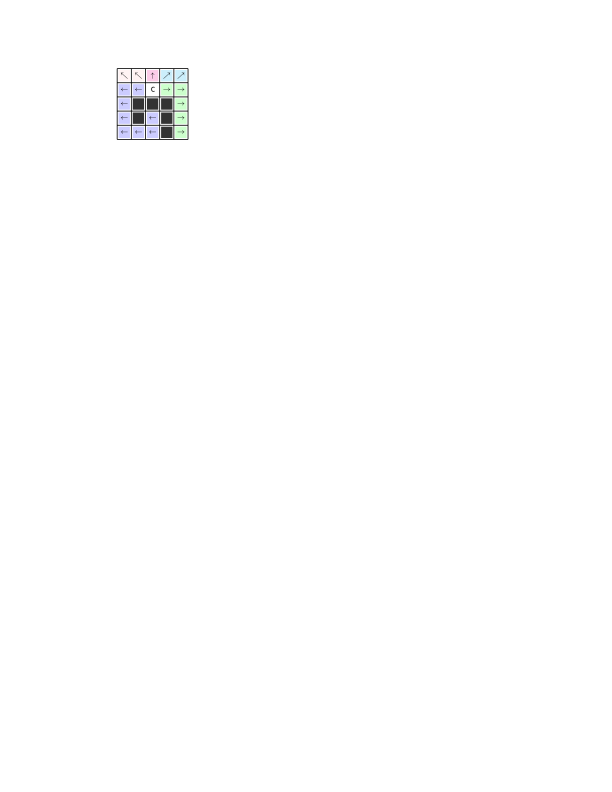
\includegraphics[width=\linewidth]{images/botea-cpd.pdf}
				\caption{Movement-grid for cell $c$\cite{botea-cpd-2013}.}
				\label{fig:cpd}
			\end{wrapfigure}
			
			The construction of a CPD\cite{botea-cpd-2013} is similarly simple.
			After solving the all-pairs shortest path problem, the result needs to be compressed.
			Uncompressed data is usually too large as the space requirement is in $\bigo{n^2}$ or even $\bigo{n^2 \log n}$ for graphs.
			A combination of compression techniques can be used to get sufficient results.
			This includes the encoding of whole areas with same movement operations, run-length encoding (RLE) and use of default values to reduce the number of explicitly stored values\cite{botea-cpd-2013}.
			Using these techniques, a compression factor of over 950 compared to an uncompressed database can be achieved.
	
\section{Geometric routing}
\label{sec:geometric-routing}

	Finding paths in a geometric domain, also called the \term{euclidean shortest path} problem, is the process of determining shortest paths through open spaces by avoiding obstacles.
	There are two main strategies to find euclidean shortest paths:
	Generate edges for graph-based routing or create a shortest paths map, a structure similar to CPDs.
	
	\subsection{Visibility graphs}
	\label{subsec:visibility-graph}
	
		The first mechanism generates edges and then uses a normal graph-based routing algorithm to actually find the shortest path.
		There are multiple ways on how to create such edges.
		One approach is the creation of a so-called \term{visibility graph}, which is a normal graph with edges between vertices that are visible to each other.
		Or in other words, for any two $u, v \in V$ there is an edge $(u, v) \in E$ if and only if there is no obstacle intersecting this edge.
		A visibility graph might become very large, in fact, the worst-case regarding the size is a complete graph with $\bigo{|V|^2}$ many edges.
		
		Alternatives to the visibility graph generation are based on Voronoi diagrams or skeletonization methods.
		However, routing results on such graphs are not necessarily optimal\cite{graser-osm-open-spaces}, since a straight edge between visible vertices is the shortest possible connection.
		
		Source and destination locations must be part of the graph and can be connected with the same algorithm used to create the graph itself.
	
	\subsection{Continuous Dijkstra}
	\label{subsec:continuous-dijkstra}
	
		The second strategy creates a map of regions starting from a source vertex $s$, which has strong similarities to a CPD.
		Each region of this map stores the predecessor vertex, which can be used to determine shortest paths by following the predecessor relations from any given location back to $s$.

		This map can also be seen as a tree with $s$ as its root and each region as a leaf.
		The creation of a shortest-path tree might remind one of Dijkstra's algorithm, which gives the \term{continuous Dijkstra} paradigm its name\cite{mitchell-discrete-geodesic}.
		
		To precisely determine these regions, one popular approach is to create \term[wavefront]{wavefronts} propagating through open spaces.
		A well-fitting analogy for this approach is the propagation of water waves traveling through a 2D space, folding around obstacles, colliding with each other and finally reaching the destination location.
		Recursively following each wave back to its origin yields the shortest path from the source to the destination.
		These wavefronts are also called \term[wavelet]{wavelets}), because they only cover a certain angular range due to collisions and the presence of obstacles.
		
		Each wavefront can collide with obstacle and other wavefronts.
		After detecting such a collision, the angular region of the wavefront is adjusted depending on the type of collision.
		For each region the origin of the wavefront is known, which enables the query routine to follow these predecessors back to the source.
		The key difficulty of this approach is the efficient detection and handling of collisions with obstacles and other wavefronts\cite{hershberger-suri}.

\section{Agent-based systems and simulations}

	Simulating complex systems with numerous autonomous individuals, called \term[agent]{agents}, is a complex task.
	Agent-based models help to break down this complexity by simulating each agent separately with its own behavior and decision-making\cite{macal-introductory-tutorial}.
	Agents interacting with the environment and other agents are an essential part of this and can in turn affect other agents and the environment.
	
	The modeling of agents can be arbitrarily complex, because agents are able to make decisions on their own making them autonomous without any controlling unit commanding them how to act.
	Even more complex agents may have a specific goal, are able to adapt themselves to their environment and thus must be able to memorize and plan things.
	
	An agent might be a simulated person but could also be a company, car or other non-living part of the simulated domain.
	Many simulations use pedestrians (or generally humans) as agents to better understand or utilize human behavior but many more scenarios with other types of agents are possible as well\cite{macal-introductory-tutorial}.

	Studying the behavior of pedestrians requires a spatial environment where agents can move and interact with each other, which requires algorithms finding optimal paths\cite{kneidl-borrmann-hartmann-navigation,gloor-hybrid-pedestrian-routing,teknomo-millonig-routing}.
	This not only includes \hyperref[sec:graph-routing]{graph-based routing} but often utilizes \hyperref[sec:geometric-routing]{geometric routing} as well\cite{kneidl-borrmann-hartmann-navigation}.
	
	\subsection{The MARS framework}
	
		The algorithm presented in this work was implemented to enhance agent-based simulations created using the framework MARS (Multi-Agent Research and Simulation).
		MARS is a C\#/.NET framework developed by the MARS group, an academic research group of the Hamburg University of Applied Sciences (HAW) in Hamburg, Germany, to create and execute agent-based simulations\cite{mars}.
		The framework offers the necessary components, algorithms and tools to create tick-based simulations consisting of multiple agents, different layers of data and numerous static entities populating the environment.
		
		The MARS framework contains several data structures and algorithms for spatial data and especially for path finding.
		This includes a class representing spatial graphs as well as the A* algorithm, which can determine shortest paths on such graphs.
		MARS also contains numerous spatial indices, mathematical operations and I/O classes, for example to serialize the trajectories of agents.
		 
		This work is based on the MARS framework to be directly usable by simulations, which is why, among other parts, the spatial graph and A* algorithm of MARS are used.
		More details on the design and implementation are given in \Cref{chap:design} and \ref{chap:implementation}.
		
	\chapter{Related work}
	\label{chap:related-work}
	
		% !TEX root = ../thesis.tex
% !TeX spellcheck = en_US

Scientific literature contains related work from many different areas, mostly from geodata, graph construction and networks as well as routing and (pedestrian) path planning.
This section gives an overview about closely related work from these areas.

% Geodata and networks
	% with some assumptions like no dollinear vertices (even though these assumptions are not necessary): Constructing the visibility graph for n-line segments in O(n²) time (Emo Welzl, 1985)
Constructing a visibility graph is an important part of this thesis, thus the construction of visibility graphs in $\bigo{n^2}$ time and space (with $n$ line segments), under the condition of no collinear coordinates and no intersecting line segments, was presented by Welzl in 1985\cite{welzl-visibility-graph}.
A few years later, Overmars and Welzl presented two new methods reducing the space complexity to $\bigo{n}$\cite{overmars-weizl-visibility-graph}.
Their new algorithms are based on Welzls earlier paper and the idea of a rotational sweep through neighboring vertices.
	
	% maybe, they use geom. routing to fill OSM gaps: Automatic extrapolation of missing road network data in OpenStreetMap (Funke, Schirrmeister, Storandt, 2015)

% Routing
	% Shortest paths among obstacles in the plane (Mitchell, 1993)
Shortly after Welzl and others published their work on visibility graphs, which can be used in combination with Dijkstra to find shortest paths, Mitchell presented a pure geometric method to find euclidean shortest paths around obstacles in the plain in 1993\cite{mitchell-shortest-path}.
He used wavefronts propagating from the source towards the target vertex.
Each origin of a wavefront can be traces back to the source giving the shortest path.
Because this algorithm solves the \term*{single-source shortest-paths} problem just like the Dijkstra algorithm does on a network, this technique is also called the \term{continuous dijkstra} paradigm.

	% An Optimal Algorithm for Euclidean Shortest Paths in the Plane (Hershberger, Suri, 1999)
	% maybe: Efficient algorithms for Euclidean shortest path and visibility problems with polygonal obstacles (Kapoor, Maheshwari, 1988)

% Pedestrian path finding
	% online routing: A Navigation Algorithm for Pedestrian Simulation in Dynamic Environments (Teknomo, Millonig, 2007)
	% maybe: pure geometric/geodesic approach with navigation fields: https://iopscience.iop.org/article/10.1088/1367-2630/12/4/043032/pdf
	% unified pedestrian routing (they use the above navigation field graph generation): A Unified Pedestrian Routing Model for Graph-Based Wayfinding Built on Cognitive Principles (Kielar, et al. 2017)
	
	\chapter{Design}
	\label{chap:design}
	
		% !TEX root = ../thesis.tex
% !TeX spellcheck = en_US

\section{Overview and Context}

	% Used by agents for wayfinding
	The primary goal of the hybrid routing algorithm is to provide a more accurate path planning for agent based simulations than normal graph based routing, which is integrated into the MARS framework.
	Such major goal implies several constrains on the architecture and design of the software.
	
	\subsection{Requirements}
	
		Functional requirements of the resulting software can be formulated quite easily, since this is not a large commercial product.
		The hybrid routing algorithm should determine an optimal path between two locations following ways and traversing open spaces based on a configurable weight function.
		Therefore, the geospatial data basis may contain a road network data and obstacles, which are features that should be avoided on paths through open spaces.
		
		More complex and time consuming are the quality requirements.
		Because this is not part of a commercial software development, these requirements were not officially and formulated.
		Nonetheless, they exist and consist of the following aspects.
	
		The largest quality requirement in terms of effort is performance.
		It affects large parts of the software architecture since the resulting algorithm, dispite its complexity, should ideally have a negligible impact on the overall performance of a simulation.
		Routing algorithms and engines often consist of two steps, a preprocessing and query answering step.
		In order to create fluent and fast simulations, the performance of answering numerous routing requests must be as good as possible.
		The time needed for preprocessing is of less relevance.
		
		A rather obvious requirement is the correctness of resulting routes.
		The answer of a routing query must return the shortest route according to a given weight function for the underlying edges.
		Even when using an approximation algorithm to determine shortest paths, the results can be checked against all other possible paths to verify the optimality of the resulting path.
		
		Another quality requirement is the closeness of the resulting routes to real pedestrian behavior.
		Unfortunately, this can hardly be measured without having extensive data of real world pedestrians in real world locations.
		However, the overall trajectory of a calculated route should ideally be identical to a real world pedestrian trajectory and should at least make sense to an observer without additional knowledge of the real world location.
		Furthermore, real pedestrian behavior is not part of the shortest path calculations but is instead a task for realistic agent modeling.

		Next to the software specific requirement, the overall code itself should of course be well documented and tested.
	
	\subsection{Constrains}
	\label{subsec:constrains}
		
		% Well integrated into MARS and NTS, no new dependencies
		One major constraint is the integration of the hybrid routing algorithm into the \term*{MARS} framework to make the use as easy as possible and to centralize the code base for better maintenance.
		This means the programming language will be C\# and because MARS uses the \term{NetTopologySuite} (\term*{NTS}) as basis for all major geospatial operations, this algorithm will be based on this library as well.
		
		The planned integration into another code base affects the management of dependencies.
		On the one hand, the amount dependencies which are not already part of the target code base should be kept to a minimum.
		On the other hand, using only libraries, on which the target code base depends as well, is not always possible due to version mismatches.
		However, the latter case can be avoided or treated in a way that the mismatch disappears or doesn't lead to compatibility problems.
	
	% Diagram with MARS Agent using my hybrid algorithm
	
\section{Components}

\section{Deployment view}

	% published in MARS

\section{Combination of routing algorithms}
\label{sec:combining-routing-algorithms}

	This section describes the core aspect of this thesis:
	The decision of a strategy to combine graph and geometric based routing algorithms.
	
	In the following subsections, four approaches are discussed of which the last one seemed to be the most promising.
	The first three are using any normal graph based routing algorithm, like A* or Dijkstra, in combination with the geometric continuous Dijkstra paradigm.
	Only the last and further pursued approach uses visibility graphs for routing.
	
	% Ad-hoc creation of edges by stopping A* and continuing with wavefront algorithm
	\subsection{Ad hoc generation of edges}
	
		The idea of an ad hoc generation of edges is the following:
		Whenever the graph routing algorithm reaches a crossing of ways, it's paused and the continuous Dijkstra algorithm is started.
		Since no target vertex is defined, the geometric routing will be stopped after the furthest wavelet reached a certain distance.
		The continuous Dijkstra approach actually creates a shortest path map, so the shortest paths of all reached vertices are calculated yielding a series of edges.
		These edges are then added to the graph for the paused graph based routing algorithm.
		
		In a real world example for this approach would be a pedestrian walking down a road but then crossing a park for a shortcut before continuing to follow the roads again.
		Doing the shortcut was not planned but an ad hoc decision just as the algorithm would do.
		
		The advantage of this approach is the realistic behavior of pedestrians not planning the route in beforehand.
		In fact Teknomo and Millonig introduced a routing mechanism for agent based simulations with the assumption of little to no apriori knowledge of agents about their environment \cite{teknomo-millonig-routing}.
		
		One disadvantage is a relatively high complexity since no standard algorithm from frequently used software frameworks support a pause functionality, so any routing algorithm has to be manually adjusted or implemented from scratch.
		
		Also this approach will likely cause performance issues.
		When using Dijkstra as graph based routing algorithm, $\bigo{|V|}$ many vertices are visited, which leads to $\bigo{|V|}$ routing requests using the geometric continuous Dijkstra algorithm.
		Because a simple caching of the shortest path map is not possible, at least not without a smart and complex caching strategy, this decreases the runtime of the whole routing process significantly.
		Even when using the continuous Dijkstra approach from Hershberger and Suri \cite{hershberger-suri} with only $\bigo{n \log n}$ time requirement, the number $n$ of vertices in obstacles is expected to be much higher than the size of $V$.
		
		Another aspect against this approach is the hypothesis that an ad hoc generation of edges will probably not change the resulting shortest path compared to a precomputed graph consisting of all possible edges.
		An argumentation for the correctness of this hypothesis can be sketched as follows.
		
		Assume that the ad hoc generation starts at each road junction vertex $j$ and stops when a certain condition is fulfilled (for example only generating paths of a certain length).
		When the graph routing algorithm reaches an unvisited junction vertex $j$ from some other vertex $v$, it either used a road edge or preprocessed edge to get there. Therefore, the following two cases exist:
		
		\begin{itemize}
			\item In case a preprocessed edge was used, then the shortest path from $v$ to $j$ would be identical when using a completely preprocessed graph containing this exact edge $(v, j)$.
			\item In case a road edge was used to get to $j$, then there are two sub-cases.
			\begin{itemize}
				\item In case the road edge was in deed the optimal path to $j$, it would have been used in a preprocessed graph as well.
				\item In case the road edge was not the optimal path, then the ad hoc generation stopped before reaching $j$ (due to the distance or any other stopping condition) and the edge $(v, j)$ was never added.
			\end{itemize}
		\end{itemize}
		
		Even though, this is not a formal proof, generating a preprocessed graph and using a normal routing algorithm is probably as least as good as using the ad hoc generation approach.
	
	% Concurrent routing: Use A* and wavefront in parallel and merge the results
	\subsection{Concurrent routing}
	
		A different approach would be two concurrent routing queries, one on the normal road graph and one using a visibility graph or a similar generated graph.
		Having the two shortest paths, one could merge them into one path, which would consist of alternating segments from the one or the other graph.
		To merge them, first determine the intersection points and for each pair of segments, choose the better one based on a weight function.
		
		The most prominent advantage is the simplicity of the routing requests, since known routing algorithms could be used.
		Therefore, it would be rather simple to implement and speed up techniques could be used.
		
		However, there is a major disadvantage, which is the uncertainty, that the two paths are actually intersecting at any point.
		Even if they are intersecting, a single intersection on a long route is not very helpful.
		Only if the two routes are intersecting frequently enough, this approach could actually result in good routes.
	
	% Concurrent routing for segments (e.g. start new routing calls every 100m)
	\subsection{Concurrent routing on smaller segments}
	
		This approach is very similar to the one above, however, it tries to fix the uncertainty of intersections between the two resulting paths.
		There are multiple ways to ensure that there are enough intersections or to otherwise guarantee small enough segments to merge.
		
		One way is to stop the routing after a certain distance stopping at the next available vertex.
		After stopping for the first time, there are two such vertices, one where the graph based routing stopped and one where the routing on the generated graph stopped.
		From each vertex, two new routing queries start and stop after a certain distance.
		This is continued until one query reaches the target.
		On the one hand, this would guarantee small enough segments for later merging, on the other hand, this results in $\bigo{2^n}$ many routing queries.
		Even though each query is short, this approach would probably not scale very well.
		
		A different approach for smaller segments would be to first get the shortest path on the road graph.
		Having this path, it is split up into $n$ segments of certain length.
		From the end vertex of each segment $s_i$, a shortest path query to the start of all other segments $s_{i+1}, s_{i+2}, ..., s_n$ is performed including one query from the end of $s_i$ to the target vertex.
		Unfortunately this results in $O(n^2)$ more routing queries.
		Finally, all these queries on the generated graph can be merged together with the query result of the road graph to form a new intermediate graph.
		Finally, one last routing query on this intermediate graph is performed to get the final optimal routing result.
		
		There are probably more possible ways to ensure a sufficient amount of segments or intersection, however, this idea was not further continued.
		
		Unfortunately, both approaches have a worse time complexity than any popular routing algorithms including pure geometric routing.
		Even though the second idea might work well for appropriate segments lengths, the complexity and definite time overhead make it an unfavorable choice.
	
	% Merge of networks
	\subsection{Merge an existing network with a visibility graph}
	
		The last approach, which is the currently used one, generates a visibility graph and merges it with the existing road graph.
		The actual merge operation is very simple:
		Whenever a road edge and a visibility edge intersect, split the edges, create a new vertex there and connect the split edges accordingly.
		
		Even though, this approach is simple and still fast, there is the disadvantage of the graph size.
		A visibility graph is large and in most cases it will contain many more edges than the road graph, which negatively affects the routing performance.
		
		Another disadvantage is the time complexity of the merge operation.
		All edges have to be considered and most edges will even be considered multiple times, depending on the number of intersections.
		This leads to a time complexity of $\Omega(|E_R| + |E_V|)$ for the routing graph edges $E_R$ and visibility edges $E_V$.
		However, a complete graph has the highest number of edge crossings, which gives the upper bound of $\bigo{|E|^2}$ for the merge operation.
		Fortunately, road networks are very sparse and often have a node degree between three and six \cite{zhao-analysis-osm-bejing}\cite{boeing-osmnx}, resulting in a much better runtime behavior.
		\todo[inline]{Maybe analyze this myself for e.g. Germany?}
		\todo[inline]{Link to possible optimizations discussed in later chapters}
		
		However, the advantages are more important.
		As already mentioned, this strategy is simple and fast, compared to the time complexities above, only makes one routing query and enabled the use of speed up methods.

	
	\chapter{Implementation}
	\label{chap:implementation}
	
		% !TEX root = ../thesis.tex
% !TeX spellcheck = en_US

This section covers details on the implementation of the previously described design.
First, an overview of the algorithm is given including a short description of used frameworks and technologies.
Second, two new and important data structures are described in detail.
Finally, each algorithmic step of the graph generation but also of the query answering is described in the main sections of this chapter.

\section{Algorithm overview}

	Before technical details are covered, this section gives a broad overview of the implementation.

	\subsection{Frameworks and technology}
	
		As mentioned in \cref{subsec:constrains} about the constrains, the used programming language is C\# due to the dependency to the MARS framework.
		The MARS framework is based on the widely used C\# library \term{NetTopologySuite} (\term*{NTS}), which contains numerous data structures, algorithms and helper function to handle and process geospatial data.
		
		Primarily, the NTS was used for basic data structures like coordinates, geometries and features but also for simple operations, e.g. the calculation of distances.
		Writing data to files is also done with the help of the NTS, namely to serialize the geospatial data into the GeoJSON format.
		
		The \term*{MARS} framework was also used for basic data structures, for example the \texttt{Position} class.
		However, higher level structures were used as well, such as \texttt{SpatialGraph} or \texttt{QuadTree} classes.
		
		Not all data structures and algorithms already existed to create the hybrid routing graph.
		Most notably, a \hyperref[subsubsec:intersection-checks]{fast line intersection check}, a \hyperref[subsec:binindex]{bin based index} and a fast \hyperref[subsec:shadow-areas]{vertex filtering method} were implemented.
		The latter one refers to the so called \emph{shadow areas} in the sections below.
		Several other helper functions and simpler structures, for instance separate classes for vertices and obstacles, were added as well.

	\subsection{Early implementation based on the continuous dijkstra paradigm}
	
		An early implementation, before the final decision for a strategy fell, was not creating a visibility graph but instead it was based on the \term*{continuous dijkstra} paradigm with wavelets propagating through open spaces.
		However, there were two reasons why this first approach was replaced by a visibility graph based algorithm.
		
		The main reason was the overall strategy decision on the visibility graph approach.
		The other reason were performance enhancement made to the naive continuous dijkstra implementation.
		
		Early stages of the continuous dijsktra approach used a very naive and simple implementation without optimizations mentioned in recent literature on this topic.
		Wavelets did not move continuously but instead they snapped to the next \enquote{event}, i.e. the next visible vertex where new wavelets can spawn.
		Because the strategy decision was not yet made at that time, no larger efforts went into optimizing the implementation, e.g. by implementing the approach presented by Hershberger and Suri\cite{hershberger-suri}.
		Instead, a simple preprocessing was introduced and lead to a major performance improvement.
		This preprocessing determined the visibility between all vertices used for the above mentioned events.
		Such predetermined visibilities are the core idea of a visibility graph, thus moving to an approach using an actual visibility graph was only a small step.
		Design decisions regarding the implementation and concrete algorithm were discussed in \cref{sec:design-decisions}.
		
		A third reason against this early continuous dijkstra implementation were the difficulties and the disadvantages of combining the network based routing with the continuous dijkstra algorithm, as described in \cref{sec:combining-routing-algorithms}.
		
		Therefore, this first continuous dijkstra approach was not further pursued but converted to a generator for a routable visibility graph.
	
%	\subsection{Chosen approach and potentially faster known algorithms}
%
%		Due to the step by step development by turning the former continuous dijkstra preprocessing into a visibility graph generator, the implemented approach does not follow algorithms described in the literature.
%		The performance of this implementation, as shown in \todo[inline]{link to evaluation chapter}, is still enough for practical use, but a well designed and fast algorithm, like the one presented by Overmars and Welzl \cite{overmars-weizl-visibility-graph} or the one by Ghosh and Mount \cite{ghosh-output-sensitive-vgraph}, would clearly increase performance.
%		However, this performance enhancement would only affect the generation of a visibility graph and not the performance of the routing queries.
			
	\subsection{Algorithm steps}
	\label{subsec:algorithm-steps}
		
		As describes in \cref{sec:components}, the \texttt{HybridVisibilityGraphGenerator} class provides a factory method to create a \texttt{HybridVisibilityGraph} from a given collection of features.
		This factory method consists of the following top level steps, which are all described in \cref{sec:visibility-graph-creation} in more detail:
		\begin{enumerate}
			\item Filter the given features for obstacles
			\item Determine the visibility neighbors
			\item Use this visibility relation to create a visibility graph
			\item Merge the existing road network into this graph
		\end{enumerate}
		The graph then allows to route between existing nodes.
		So far, routing queries between arbitrary locations cannot be answered, since this graph based approach only allows routing between existing nodes.
		To enable answering routing requests between arbitrary locations the resulting graph needs to be extended with edges from and to the given start and end locations.
		These edges are themselves visibility edges and can therefore be created just like the visibility edges before. The process is further described in \cref{sec:answering-queries} and contains the following steps:
		\begin{enumerate}
			\item Connect the source coordinate to the graph:
			\begin{enumerate}
				\item Add a node to the graph at the source coordinate
				\item Determine the visibility edges to and from the source coordinate
			\end{enumerate}
			\item Repeat the steps for the destination coordinate
			\item Route along the resulting graph
			\item Restore the original graph by removing all added nodes and edges
		\end{enumerate}
		The last step ensures that subsequent routing queries are answered based on the original graph and not on a previously altered version.
		It also prevents an uncontrolled growth of the graph.
	
\section{Data structures}
	
	Before the separate steps of the graph generation are described in detail, the newly created data structures are presented.
		
	\subsection{Shadow areas}
	\label{subsec:shadow-areas}
		
		Shadow areas are a method to quickly determine vertices that are definitely not visible to each other.
		The idea of shadow areas is the following:
		Let $v$ be the currently processed vertex and think of it as a light bulb illuminating its surroundings.
		An obstacle $o$ casts a shadow outwards and everything within this shadow is definitely not visible from $v$.
		
		Each shadow is determined by three values: two values for the angular range and a third value for the minimum distance from which other vertices within the angular range are definitely not visible.
		This means each shadow is an interval with of certain distance, which turns the visibility problem into an interval intersection problem.
		Latter one, specifically to check whether a point is within an angle area, can be solved using just a few arithmetic operations.
		
		The angular range of a shadow is determined by the two bounding vertices (marked in red in \cref{fig:shadow-area}) of the respective obstacle.
		The furthest of these two bounding vertices determines the minimum distance of the shadow area.
		
		Keeping track of these shadow areas for each vertex significantly improves performance, especially with the use of the \texttt{BinIndex} data structure described \hyperref[subsec:binindex]{below}.
		\todo[inline]{conrete numbers?}
		
		% NetworkRoutingPlayground->Jungfernstieg dataset with 7916 vertices: ~7.3s with and 67s without shadow areas -> speed up of factor ~9
		% Hamburg inner city dataset with 67819 vertices: 382s with and ~31000s without shadow areas -> speed up of factor ~81
		
		\begin{figure}[h]
			\begin{figcenter}
				\begin{tikzpicture}
					\def\angle{20}
					\def\boundingVertexDistance{3}
					
					\tikzDot[label=$v$]{(0,1.5)}{v}
					\coordinate (shadow-arc-top)				at ($(v) +( \angle:\boundingVertexDistance)$);
					\coordinate (shadow-arc-bottom)				at ($(v) +(-\angle:\boundingVertexDistance)$);
					\coordinate (shadow-arc-top-end)			at ($(v) +( \angle:5.75)$);
					\coordinate (shadow-arc-bottom-end)			at ($(v) +(-\angle:5.75)$);
					\coordinate (shadow-arc-top-faded-end)		at ($(v) +( \angle:6.5)$);
					\coordinate (shadow-arc-bottom-faded-end)	at ($(v) +(-\angle:6.5)$);
					
					% Gray area
					\filldraw[lightgray] 
					(shadow-arc-bottom) arc [start angle=-\angle, delta angle=2*\angle, radius=\boundingVertexDistance] --
					(shadow-arc-top-end) --
					(shadow-arc-bottom-end) --
					cycle;
					\draw[gray]
					(shadow-arc-bottom-end) --
					(shadow-arc-bottom) arc [start angle=-\angle, delta angle=2*\angle, radius=\boundingVertexDistance] --
					(shadow-arc-top-end);
					
					\draw[dotted] (v) -- (shadow-arc-top);
					\draw[dotted] (v) -- (shadow-arc-bottom);
					
					% Faded gray area
					\filldraw[draw=none,lightgray,path fading=east]
					(shadow-arc-top-faded-end) --
					(shadow-arc-top-end) --
					(shadow-arc-bottom-end) --
					(shadow-arc-bottom-faded-end) --
					cycle;
					\draw[gray,path fading=east] (shadow-arc-top-end) -- (shadow-arc-top-faded-end);
					\draw[gray,path fading=east] (shadow-arc-bottom-end) -- (shadow-arc-bottom-faded-end);
					
					% Obstacle 1
					\tikzDot[red]{(shadow-arc-top)}{o10}
					\tikzDot{(3.5,2)}{o11}
					\tikzDot[red]{($(v) +(-\angle:1.2)$)}{o12}
					\node[above right = 0.5 and 1 of o12] {$o_1$};
					
					% Obstacle 2
					\tikzDot[label=right:$v'$]{(3.5,1.35)}{o20}
					\tikzDot{(3.5,-0.25)}{o21}
					
					% Obstacle 3
					\tikzDot[label=right:$v''$]{(2.1,1.1)}{o30}
					\tikzDot{(2.1,-0.5)}{o31}
					
					\node[darkgray] at (4.65,1.5) {\huge$S$};
					
					\draw (o10) -- (o11) -- (o12) -- (o10);
					\draw (o20) -- node[right] {$o_2$} (o21);
					\draw (o30) -- node[left] {$o_3$} (o31);
				\end{tikzpicture}
			\end{figcenter}
			\caption{Shadow area $S$ cast by obstacle $o_1$ seen from vertex $v$. The vertex $v'$ of obstacle $o_2$ is not visible from $v$ since it lies inside the shadow area. The two red vertices of obstacle $o_1$ are the bounding vertices determining angle range and distance of $S$. Note that $v''$ is not visible from $v$ even though it is not inside the shadow area.}
			\label{fig:shadow-area}
		\end{figure}
		
	\subsection{BinIndex data structure}
	\label{subsec:binindex}
		
		The \texttt{BinIndex} class implements a linear bin based index structure to store and access intervals.
		It contains $n$ many bins covering a certain range and consisting of a linked list.
		When an item is added, it is added to each bin intersecting with the range of the item.
		Due to the linked list as the underlying data structure for the bins, queries can be answered in linear time.
		\Cref{fig:bin-index} illustrates this data structure with a simple example.
		
		\begin{figure}[h]
			\begin{figcenter}
				\begin{tikzpicture}
					\def\l{0.5}
					\def\countX{9} % One more is added due to start at x=0
					\def\countY{1} % One more is added due to start at x=0
					
					\def\itemBStartX{1.5}
					\def\itemBIndexStart{1}
					\def\itemBLength{4.2}
					
					\def\itemAStartX{4}
					\def\itemAIndexStart{4}
					\def\itemALength{7.8}
					
					% Item A: Bins 1-5
					\filldraw[pattern=north west lines,pattern color=Red2] (\itemBStartX*\l,\countY+4*\l) rectangle node[above right=0.125 and -1.3]{Item B: \itemBStartX\ - 5.7} ++(\itemBLength*\l,0.5*\l);
					
					% Item B: Bins 4-11(2)
					\filldraw[pattern=crosshatch dots,pattern color=DodgerBlue3] (\itemAStartX*\l,\countY+3*\l) rectangle node[above right=0.125 and -0.5]{Item A: \itemAStartX\ - 10.8} ++(\itemALength*\l,0.5*\l);
					
					\draw[->] (0.5*\countX*\l,\countY+2.25*\l) -- +(0,-1*\l);
					
					% Draw pattern to bins
					\fill[pattern=north west lines,pattern color=Red2] (\itemBIndexStart*\l,1.5*\l) rectangle ++(\l,\l);
					\fill[pattern=north west lines,pattern color=Red2] (\itemBIndexStart*\l+1*\l,0) rectangle ++(2*\l,\l);
					\fill[pattern=north west lines,pattern color=Red2] (\itemBIndexStart*\l+3*\l,1.5*\l) rectangle ++(\l,\l);
					\fill[pattern=north west lines,pattern color=Red2] (\itemBIndexStart*\l+4*\l,1.5*\l) rectangle ++(\l,\l);
					
					\fill[pattern=crosshatch dots,pattern color=DodgerBlue3] (\itemAIndexStart*\l,0) rectangle ++(6*\l,\l);
					\fill[pattern=crosshatch dots,pattern color=DodgerBlue3] (0,0) rectangle ++(2*\l,\l);
					
					% Draw outlines of bins
					\foreach \x in {0,...,\countX}
					{
						\draw (\l*\x,0) rectangle ++(\l,\l);
					}
					
					\draw (\itemBIndexStart*\l,1.5*\l) rectangle ++(\l,\l);
					\draw[->] (\itemBIndexStart*\l+0.5*\l,\l) -- ++(0,0.5*\l);
					
					\draw (\itemBIndexStart*\l+3*\l,1.5*\l) rectangle ++(\l,\l);
					\draw[->] (\itemBIndexStart*\l+3.5*\l,\l) -- ++(0,0.5*\l);
					
					\draw (\itemBIndexStart*\l+4*\l,1.5*\l) rectangle ++(\l,\l);
					\draw[->] (\itemBIndexStart*\l+4.5*\l,\l) -- ++(0,0.5*\l);
					
					% Label
					\foreach \x in {0,...,\countX}
					{
						\node at (\l*\x+0.5*\l,-0.35) {$\x$};
					}
					
					\node at (0.5*\countX*\l,-0.875) {bins};
					\node[align=right] at (-1.25,0.5*\countY*\l+\l) {Linked list\\of bins};
				\end{tikzpicture}
			\end{figcenter}
			\caption{Bin index filled with two items A and B. Since item A was added first, B's entries in, which fall into a bin where en entry for item A already exists, are moved to a next item in the linked list of the bin. Each bin covers a range, which means non integer value are rounded down (for from-values) or up (for to-values).}
			\label{fig:bin-index}
		\end{figure}
		
		The NetTopologySuite offers several indices specifically made for intervals, namely the \texttt{BinTree}, \texttt{SIRtree} and \texttt{SortedPackedIntervalRTree}, of which only the first one is dynamic and thus allows insertions and deletions after the first query was made.
		Even though these three data structures are tree based and should offer a logarithmic query time complexity compared to the linear time complexity of the \texttt{BinIndex}, the simple and list based \texttt{BinIndex} is significantly faster even for larger datasets with tens of thousands of vertices.
		It is thinkable that the logarithmic complexity is useful for even larger datasets with millions of vertices.
		
		\todo{Performance analysis (maybe in evaluation chapter?)}
		
\section{Routing graph creation}
\label{sec:visibility-graph-creation}
		
	This section describes the steps given in \cref{subsec:algorithm-steps}, generating a visibility graph and merging it with a road network, in more detail.

	\subsection{Step 1: Obstacle filtering and feature preprocessing}
	\label{subsec:step-1-preprocessing}
			
			First the features are filtered to get all relevant obstacle features, which are of arbitrary shape.
			For performance reasons, multi-geometries, like \texttt{MultiPolygon} are split up into their separate geometries.
			This is unproblematic for \texttt{MultiLineString} as well as \texttt{MultiPolygon} features, since holes in a polygon are not reachable in the first place and unwrapping the \texttt{MultiPolygon} will not change this.
			
			Point features are also considered so that visibility edges can reach \term*{points of interest}.
			Of course the later performed visibility checks can ignore point features, since they have no spatial size.
			
			Another task within this first step is the triangulation of all polygonal shapes.
			The main reason is a better performance for intersection checks, which is an important operation when checking if an obstacle is between two vertices.
			Details on this intersection check implementation are described \hyperref[subsubsec:intersection-checks]{below}.
			
			Also worth mentioning is the determination of the convex hull of each obstacle.
			Of course this is not a complex task, since all obstacles are either trianges, linestrings or points, but only vertices on the convex hull of obstacles are further processed.
			
	\subsection{Step 2: Determining $k$ nearest visible neighbors}
			
			After having all preprocessed obstacles, the main task of the visibility graph creation is performed, namely the determination of all $k$ many visible neighbors.
			Determining all visible neighbors would also be possible, but this parameter is an easy way to increase performance with the downside of not having all possible edges in the final routing graph.
			
			\subsubsection{Parameter $k$ and consequences on the shortest paths}
			
				The $k$, however, is not just a single parameter, but rather consists of two separate values:
				The number of bins $k_b$ and the number of maximum neighbors per bin $k_n$.
				This means a maximum of $k_b \cdot k_n$ many neighbors are considered.
				
				Each bin covers a certain angle area of each vertex, for example for a bin count of 36, each bin would cover a 10° area.
				In fact, the chosen default values of 36 bins with ten neighbors per bin worked well in all and usages of the implementation.
				When a bin is filled and a new edge should be inserted, an existing edge might be removed from the bin.
				The criterion on which edge to remove is its length such that only the $k_n$ shortest edges per angle area of the bin remain.
				
				Without this subdivision and by only considering a static maximum number of neighbors, it is possible to only have edges to complex and close objects but no edges to obstacles further away.
				An example for this would be a large and open park where the $k$ nearest neighbors are probably all at the side of the park where the currently processed vertex is, even though the far away other side of the park is clearly visibly.
				This subdivision into bins ensures that there will definitely be connections to the other side of the park.
				
				Not considering exactly all edges leads to less accurate routing results, i.e. to suboptimal non-shortest paths.
				As mentioned above, a bin only contains the $k_n$ shortest edges.
				In the case of using the above mentioned default values of ten edges per 10° range, an omitted edge led to a similar direction as at least nine other edges did.
				The negative influence of a detour to the total route length by using the second-best edge towards the destination is most likely not significant.
				\todo{Check this in evaluation! Test: ca. 17\% of edges are removed with $(36,10)$ compared to $(3600,1000)$ with only 13\% longer calculation time}
			
			\subsubsection{Terminology}
			
				Before describing the details on determining the $k$ nearest neighbors, there are some terms that need to be defined.
				
				\begin{description}
					\item[obstacle] An obstacle is a geometry that should be avoided when determining shortest paths. It can be any type of geometry, not only a polygon.
					\item[\term*{visibility neighbor}] A visibility neighbor of a vertex $v$ is another vertex $u$, which is visible. In other words a linestring from $v$ to $u$ does not intersect with any obstacle. Sometimes $u$ is just called a \emph{visible neighbor}.
					\item[\term*{obstacle neighbor}] This is a vertex $u$ with an existing edge to or from the currently processed vertex $v$. In other words, $u$ is visible from $v$ but via an existing obstacle edge.
					\item[\term*{valid angle area}] Certain angle areas around a vertex in which potential visibility neighbors are checked.
				\end{description}
				
			\subsubsection{Convex hull}
				
				As mentioned above, only visibility neighbors of vertices lying on the convex hull of any obstacle are determined.
				Such a visibility neighbors also has to be on any convex hull, which means vertices not being on any convex hull will never be connected to anything.
				
				The reason for this filtering is quite simple:
				Vertices not being on a convex hull will never be part of a route since the convex hull itself is by definition the smallest set of points which area completely contains all other points \cite[2]{de-berg-computational-geometry}.
				Interpreting the convex hull as path around a shape and together with the triangle inequality, this implies that the convex hull is the shortest path around the shape.
				When determining shortest paths, the part of a route bending around an obstacle will therefore always be a subset of its convex hull.
				
				Of course, a routing query might start within a concave part of the obstacle or somewhere completely else.
				This case, however, is independent of the graph generation and belongs to answering routing queries, which is covered later in \cref{sec:answering-queries}.
				
			\subsubsection{Valid angle areas}
				
				As mentioned above, a subsection of a shortest path bending around an obstacle always follows a part of the obstacle's convex hull.
				Eventually the path switches from following the convex hull to following a visibility edge.
				
				This means, a shortest path consists of many convex hull parts that either are connected by straight lines or touch each other.
				Connecting lines between two convex hull parts always follow the clockwise or counter clockwise rotation of the convex hull segments being part of the shortest path as illustrated in \cref{fig:convex-hull}.
				In other words, if the destination vertex of the connecting line would be part of the source obstacle, then the connecting line would be part of the convex hull as well.
				Adding this target vertex would therefore enlarge the convex hull in a way that the source vertex, where the connecting line starts, will still be part of the obstacle's convex hull.

				\begin{figure}[h]
					\begin{figcenter}
						\begin{tikzpicture}
							\coordinate (c00) at (0,0.4);
							\draw (c00)
								-- ++(2.75,-0.2) coordinate (c01)
								-- ++(0.8,0.4) coordinate (c02)
								-- ++(0.1,0.8) coordinate (c03)
								-- ++(-2,0) coordinate (c04)
								-- ++(-1.4,-0.35) coordinate (c05)
								-- (c00);
							\node[above right = 0.3 and 1.6 of c00] {$o_1$};
								
							\coordinate (c10) at (2.5,3.85);
							\draw (c10)
								-- ++(-0.4,-0.4) coordinate (c11)
								-- ++(0.1,-0.6) coordinate (c12)
								-- ++(2.8,0) coordinate (c13)
								-- ++(-0.4,1.2) coordinate (c14)
								-- (c10);
							\node[below right = 0.3 and 0.5 of c10] {$o_2$};
							
							\def\d{1.5\pgflinewidth}
							\filldraw[thin,Green4!35!white] ($(c03)+(0,\d)$) -- +(180:0.35) arc [start angle=180, delta angle=-97.126, radius=0.35];
							\draw[thin,Green4] (c03) -- (intersection of c03--[shift=(c03)]82.874:3 and c12--c13);
							\draw[thin,Green4] ($(c03)+(0,\d)$) -- +(180:4);
%							
							\filldraw[thin,DodgerBlue3!35!white] ($(c12)+(0,-\d)$) -- +(279.462:0.4) arc [start angle=279.462, delta angle=80.538, radius=0.4];
							\draw[thin,DodgerBlue3] (c12) -- (intersection of c12--[shift=(c12)]279.462:1 and c03--c04);
							\draw[thin,DodgerBlue3] ($(c12)+(0,-\d)$) -- +(0:4);
							
							\tikzDot[label={right:$s$}]{(c01)}{s}
							\tikzDot[label={right:$v_0$}]{(c03)}{v0}
							\tikzDot[label={left:$v_1$}]{(c12)}{v1}
							\tikzDot[label={below:$v_2$}]{(c13)}{v2}
							\tikzDot[label={left:$t$}]{(c10)}{t}
							
							\draw[->,Red2,thick] (s) -- (c02);
							\draw[->,Red2,thick] (c02) -- (v0);
							\draw[->,Red2,thick] (v0) -- (v1);
							\draw[->,Red2,thick] (v1) -- (c11);
							\draw[->,Red2,thick] (c11) -- (t);
						\end{tikzpicture}
					\end{figcenter}
					\caption{The path from $s$ via $v_0$ and $v_1$ to $t$ bends along the convex hulls of $o_1$ and $o_2$.
						The segment from $v_0$ to $v_1$ is a connecting line between the hull parts.
						% Suppose $v_1$ would be part of $o_1$, then the path from $s$ via $v_0$ to $v_1$ would be on its convex hull. Same holds true for $v_0$ and $o_2$ respectively.
						\\
						The green angle at $v_0$ indicates the angle area in which all visibility neighbors of $v_0$, in case they would be added to $o_1$, would enlarge $o_1$'s convex hull without removing $v_0$ from it. Same applies to the blue angle for $o_2$ and $v_1$ respectively.
						\\
						Vertex $v_2$, however, is not a potential neighbor for $v_0$.
						Adding it to $o_1$ would not only remove $v_0$ from its convex hull but also from the shortest path.}
					\label{fig:convex-hull}
				\end{figure}
				
				The marked green and blue angle areas in \cref{fig:convex-hull} represent the \term{valid angle areas} for potential visibility neighbors.
				Vertices at other angles will be ignored since the resulting edges will never be part of a shortest path.
			
			\subsubsection{Visibility graph generation overview}
			
				The performed steps of determining the visible neighbors are the following.
				Each step is described with more details sections below.
				\begin{enumerate}
					\item Determine the obstacle neighbors for each vertex.
					\item For each vertex $v$ lying on the convex hull of any obstacle, determine its visibility neighbors as follows.
					\begin{enumerate}
						\item For each other vertex $u$, do the following:
						\begin{enumerate}
							\item Is $u$ in any shadow area \emph{or} not on any convex hull \emph{or} not in any valid angle area? If so: $u$ is not relevant, move to the next other vertex.
							\item Query all obstacles between $v$ and $u$. This is done by the bounding box spanned by $v$ and $u$.
							\item Create and store the shadow area of each such obstacle $o$.
							\item Check if $u$ is a visibility neighbor, which is true if $u$ is a) still not in any shadow area and b) the line segment from $v$ to $u$ intersects with none of the above queries obstacles.
						\end{enumerate}
						\item Sort visibility neighbors into bins based on the obstacle neighbors.
					\end{enumerate}
				\end{enumerate}
			
			\subsubsection{Determining obstacle neighbors}
				
				% TODO Revise this and maybe add more details
				Determining the obstacle neighbors is relatively simple and straight forward.
				Each coordinate $c$ of an obstacle $o$ is processed by looking at the previous and next coordinates $c_p$ and $c_n$ on that obstacle, which are the potential neighbors.
				If the line segment $(c, c_p)$ to the previous coordinate, for $c_n$ respectively, does not intersect with any obstacle, it is considered an obstacle neighbor.
				
				\begin{figure}[h]
					\begin{minipage}[t]{0.475\textwidth}
						\begin{figcenter}
							\begin{tikzpicture}
								\tikzDot[label={[text=gray]below:$v_0$},gray]{(0,0)}{v0}
								\tikzDot[label=above:$v_1$]{(1,1.5)}{v1}
								\tikzDot[label=below:$v_2$]{(2,0)}{v2}
								\tikzDot[label=above:$v_3$]{(3,1.5)}{v3}
								\tikzDot[label={[text=gray]below:$v_4$},gray]{(4,0)}{v4}
								
								\draw[gray] (v0) -- (v1);
								\draw[->] (v2) -- (v1);
								\draw[->] (v2) -- (v3);
								\draw[gray] (v3) -- (v4);
							\end{tikzpicture}
						\end{figcenter}
						\caption{The black lines show the obstacle neighbors of $v_2$, which are $v_1$ and $v_3$.}
					\end{minipage}
					\hfill
					\begin{minipage}[t]{0.475\textwidth}
						\begin{figcenter}
							\begin{tikzpicture}
								\def\d{1.5}
								
								\tikzDot[gray]{(0,0)}{c00}
								\tikzDot[label=above:$v_0$]{(0,\d)}{v0}
								\tikzDot[label=above:$v_1$]{(\d,\d)}{v1}
								\tikzDot[label=above:$v_2$]{(2*\d,\d)}{v2}
								\tikzDot[label={[text=gray]below:$v_3$},gray]{(\d,0)}{v3}
								\tikzDot[gray]{(2*\d,0)}{c20}
								
								\node at (0.5*\d,0.5*\d) {$o_1$};
								\node at (1.5*\d,0.5*\d) {$o_2$};
								
								\draw[gray] (c00) -- (v0);
								\draw[gray] (c00) -- (v3);
								\draw[->] (v1) -- (v0);
								\draw[->] (v1) -- (v2);
								\draw[->,gray] (v1) -- (v3);
								\draw[gray] (c20) -- (v3);
								\draw[gray] (c20) -- (v2);
							\end{tikzpicture}
						\end{figcenter}
						\caption{The black lines show the obstacle neighbors of $v_1$, which are $v_0$ and $v_2$. The vertex $v_3$ is a neighbor as well, but hidden due to the touching obstacles $o_1$ and $o_2$.}
					\end{minipage}
				\end{figure}
			
			\subsubsection{Line segment intersection checks}
			\label{subsubsec:intersection-checks}
			
				All intersections are checked using own implementations no not rely on the generalized and therefore slower intersection checks of the NetTopologySuite.
				In fact, there are two types of intersection checks implemented:
				One check for intersection between two arbitrary line segments and one checks if a point lies within a triangle.
				This triangle check is used for closed obstacles, which got triangulated during \hyperref[subsec:step-1-preprocessing]{preprocessing}.
				
				The line segment intersection check uses a cross product based approach described in \emph{Introduction to algorithms} by Thomas H Cormen et al \cite[1018]{cormen-introduction-to-alg}.
				Even though this method only works on single line segments, it is significantly faster than general purpose checks provided by the NetTopologySuite.
				
				\begin{figure}[h]
					\begin{figcenter}
						\begin{tikzpicture}
							\tikzDot[label={below left:$(1,0,0)$}]{(0,0)}{a}
							\tikzDot[label={below right:$(0,1,0)$}]{(4,0)}{b}
							\tikzDot[label={above:$(0,0,1)$}]{(2,3)}{c}
							
							\coordinate[between={a and c}] (ac);
							\coordinate[between={b and c}] (bc);
							\coordinate[between={a and b}] (ab);
							
							\draw (a) -- (b);
							\draw (a) -- (c);
							\draw (b) -- (c);
							
							\draw[dotted] (a) -- (bc);
							\draw[dotted] (b) -- (ac);
							\draw[dotted] (c) -- (ab);
							
							\tikzDot{(intersection of a--bc and b--ac)}{center};
							\node[below=1mm of center,inner sep=0mm,fill=white] {$c=(\nicefrac{1}{3},\nicefrac{1}{3},\nicefrac{1}{3})$};
							
							\tikzDot[label={left:$a=(0.5,0,0.5)$}]{(ac)}{left}
							\tikzDot[label={right:$b=(-0.2,0.5,0.7)$}]{(3.4,2.1)}{right}
						\end{tikzpicture}
					\end{figcenter}
					\caption{A triangle with barycentric coordinates and dotted lines for the three coordinate axes. Noteworthy is coordinate $b$ as it is outside the triangle, which can be directly seen from the negative value $-0.2$.}
					\label{fig:barycentric-triangle}
				\end{figure}
				
				\noindent Checking if a vertex lies inside a triangle is done by a barycentric collision check.
				This method creates a barycentric coordinate system where each coordinate has the form $(\lambda_1,\lambda_2,\lambda_3)$ of which one value is one and the other two are zero for each corner vertex of the triangle.
				\Cref{fig:barycentric-triangle} illustrates this with some exemplary points.
				Due to the properties of this coordinate system, a point $p$ is inside the triangle when the condition $0 < \lambda_i < 1$ is satisfied for each of the three values.
				Even though it sounds complex to create a whole coordinate system for a single collision check, this method only uses a few basic arithmetic operations and is therefore very fast.
				
			\subsubsection{Shadow area operations}
				
				The shadow areas are stored in the previously described \hyperref[subsec:binindex]{BinIndex} data structure.
				Inserting therefore works as describes above.
				
				Shadow areas are always relative to a central vertex $v$.
				Checking if a different vertex $u$ is within any shadow area, and therefore not visible from $v$, is quite simple.
				First, all shadow areas are queried that fall into the bin of the vertex's angle.
				Second, for each shadow area $s$ it is checked whether $u$ is at least a far away from $v$ as the minimum distance of $s$ and whether the vertex is exactly within the angle area of $s$.
				If both holds true for any such shadow area, then $u$ is not visible from $v$.
				
			\subsubsection{Determining visibility neighbors}
			
				The \texttt{VisibilityGraphGenerator} class contains the above described method and structures to determine the visibility neighbors for every vertex.
				Essential to this process is the \texttt{GetVisibilityNeighborsForVertex} method determining the visibility neighbors for a single vertex.
				
				This method uses the concept of shadow areas stored in a BinIndex structure with a bin count of 360, each bin covering a 1° area.
%				Additionally, all obstacles casting a shadow are separately stored, simply to check whether or not a obstacle already casts a shadow.
%				Since querying of obstacles is necessary, they are stored in a QuadTree.
				
				For a given vertex $v$ any other vertex $u$ is checked for visibility by executing the following steps:
				\begin{enumerate}
					\item Check if $u$ is in a shadow area \emph{or} if $u$ is outside a valid angle area and continue with the next vertex if this is the case.
					\item Query all obstacles in the extent spanned by $v$ and $u$. For each obstacle $o$ the following steps are performed:
					\begin{enumerate}
						\item Get or create the shadow area for $o$.
						\item If $u$ is not part of $o$ \emph{and} a new shadow area $S$ was just created, check if $u$ is in $S$:\label{itm:if-u-not-on-obstacle}
						\begin{enumerate}
							\item If so, mark $u$ as hidden and skip all subsequent checks and obstacles.
							\item If not, mark $u$ as hidden if $u$ is within the angle area of the obstacle \emph{and} an intersection check was positive (using the methods described above in \emph{\nameref{subsubsec:intersection-checks}}).\label{itm:real-visibilty-check}
						\end{enumerate}
					\end{enumerate}
					\item If $u$ has been marked as hidden, continue with the next vertex.
					\item If $u$ is visible, store it in a bin for its angle and continue with the next vertex
				\end{enumerate}
				Most steps are relatively straightforward, however, step \ref{itm:if-u-not-on-obstacle} might not be obvious.
				For a potential neighbor $u$ being part of the current obstacle $o$, the visibility from $v$ cannot solely be determined by the shadow area of $o$.
				Imagine $o$ being a zig-zag line and $u$ being one vertex in the middle of it such that it is not visible from $v$.
				In such case, the shadow area of $o$ might start behind $u$, which means $u$ is not within the shadow area and therefore might appear visible to $v$, even though its not, when just checking via the shadow area.
				To avoid such false positive results, vertices on a current obstacle $o$ are always checked with a full visibility check in step \ref{itm:real-visibilty-check}.
			
				Having all visibility neighbors according to the amount and size of the bins, they are sorted in new bins based on the obstacle neighbors.
				This procedure is described in the following section and its result is stored for the graph creation, which is described below in \cref{subsec:step-3-graph-creation}.
			
			\subsubsection{Sort resulting visibility neighbors into bins}
			
				A naive approach to create a visibility graph would be to create edges between vertices that are visible to each other.
				This would make routing through line based obstacles possible as \cref{fig:routing-through-line-obstacle} illustrates.
				Such routing behavior is of course not correct.
				
				\begin{figure}[h]
					\begin{figcenter}
						\begin{tikzpicture}
							\tikzDot{(2,0)}{vo0};
							\tikzDot[label={[label distance=-1.25mm]above right:$v $}]{(2,1)}{vo1};
							\tikzDot{(2,2)}{vo2};
							
							\draw (vo0) -- (vo1);
							\draw (vo1) -- (vo2);
							
							\tikzDot[label=left:$n_a$,outer sep=0.5mm]{(0.5,1.3)}{n1};
							\tikzDot[label=right:$n_b$,outer sep=0.5mm]{(3.5,1)}{n2};
							
							\draw[dotted] (n1) -- (vo1);
							\draw[dotted] (vo1) -- (n2);
							
							\draw[dotted] (n1) -- (vo0);
							\draw[dotted] (n1) -- (vo2);
							\draw[dotted] (n2) -- (vo0);
							\draw[dotted] (n2) -- (vo2);
						\end{tikzpicture}
						\hspace{2cm}
						\begin{tikzpicture}
							\def\r{0.85mm}
							\def\rMargin{1.1mm} % = r + 0.25mm
							\def\gap{0.1875mm}
							
							\tikzDot{(2,0)}{vo0};
							\node (vo1) at (2,1) {};
							\node[label={[label distance=-1.25mm]above left:$v_a$}] at (vo1) {};
							\node[label={[label distance=-1.25mm]above right:$v_b$}] at (vo1) {};
							\coordinate (vo11) at ($(vo1)+(180:\rMargin)$);
							\coordinate (vo12) at ($(vo1)+(0:\rMargin)$);
							\tikzDot{(2,2)}{vo2};
							
							\filldraw (vo1)++(-\gap,0)++(90:\r) arc (90:270:\r);
							\filldraw (vo1)++( \gap,0)++(90:\r) arc (90:-90:\r);
							
%							\draw (vo1)++(270:\rMargin) -- (vo0);
							\draw ($(vo1)+(270:\r)+(-0.275mm,0)$) -- ($(vo0)+(-0.275mm,2mm)$) -- (vo0.north);
							\draw ($(vo1)+(270:\r)+( 0.275mm,0)$) -- ($(vo0)+( 0.275mm,2mm)$) -- (vo0.north);
%							\draw (vo1)++(90:\rMargin) -- (vo2);
							\draw ($(vo1)+(90:\r)+(-0.275mm,0)$) -- ($(vo2)+(-0.275mm,-2mm)$) -- (vo2.south);
							\draw ($(vo1)+(90:\r)+( 0.275mm,0)$) -- ($(vo2)+( 0.275mm,-2mm)$) -- (vo2.south);
							
							\tikzDot[label=left:$n_a$,outer sep=0.5mm]{(0.5,1.3)}{n1};
							\tikzDot[label=right:$n_b$,outer sep=0.5mm]{(3.5,1)}{n2};
							
							\draw[dotted] (n1) -- (vo11);
							\draw[dotted] (vo12) -- (n2);
							
							\draw[dotted] (n1) -- (vo0);
							\draw[dotted] (n1) -- (vo2);
							\draw[dotted] (n2) -- (vo0);
							\draw[dotted] (n2) -- (vo2);
						\end{tikzpicture}
					\end{figcenter}
					\caption{
						Both illustrations show two neighboring vertices $n_a$ and $n_b$ around a vertical obstacle with one vertex in the middle through which routing should \emph{not} be possible.
						The dotted edges are visibility edges added during graph generation.
						\\
						\underline{Left}:
						Visibility graph with naive connections.
						The two dotted visibility edges $(n_a, u)$ and $(u, n_b)$ allow the shortest path to go through the obstacle from $n_a$ via $u$ to $n_b$.
						\\
						\underline{Right}:
						The visibility graph with connection respecting the obstacles. Instead of a single node $u$, two nodes $v_a$ and $v_b$ are created.
						All gabs are for illustration purposes only, the two created nodes have the exact same location, which holds true for the parallel vertical edges.
						The node $v_a$ is connected to $n_a$ and $v_b$ to $n_b$ but $v_a$ and $v_b$ are not connected.
						This ensures that the shortest path from $n_a$ to $n_b$ does not lead through the middle vertex of the obstacle anymore.
					}
					\label{fig:routing-through-line-obstacle}
				\end{figure}
				
				It must therefore be known which visibility relations are between which obstacle neighbors.
				Knowing this enables the graph generation to distinguish between all the edges and makes a correct routing results possible.
				More on this in the \cref{subsec:step-3-graph-creation} below.
				
				Each of the resulting bins of a vertex $v$ covers the area between two adjacent obstacle neighbors.
				All visibility neighbors are sorted into these bins, which is a simple and easy process.
				
				\begin{figure}[h]
					\begin{figcenter}
						\begin{tikzpicture}
							\def\d{0.03}
							
							\tikzDot[label=below:$v$]{(0,0)}{v}
							
							\tikzDot[label=left:$n_1$]{(-2.25,0)}{n1}
							\tikzDot[label=above:$n_2$]{(0,2)}{n2}
							\tikzDot[label=right:$n_3$]{(2.25,0)}{n3}
							
							\draw[lightgray] (v) -- (n1);
							\draw[lightgray] (v) -- (n3);
							\draw[lightgray] (v) -- (n2);
							
							% Visibility edges to n1
							\tikzDot[DodgerBlue3]{(-1.1,-0.25)}{vn1}
							\tikzDot[DodgerBlue3]{(-1.6,-0.9)}{vn2}
							\tikzDot[DodgerBlue3]{(1.6,-0.5)}{vn3}
							\draw[DodgerBlue3,densely dashed,->] (v) -- (vn1);
							\draw[DodgerBlue3,densely dashed,->] (v) -- (vn2);
							\draw[DodgerBlue3,densely dashed,->] (v) -- (vn3);
%							\draw[DodgerBlue3,densely dashed,->] ($(v)+(-0.075,-\d)$) -- ($(n1)+(0.075,-\d)$);
%							\draw[DodgerBlue3,densely dashed,->] ($(v)+(0.075,-\d)$) -- ($(n3)+(-0.075,-\d)$);
							
							% Visibility edges to n3
							\tikzDot[Red2]{(0.7,1.4)}{vn4}
							\tikzDot[Red2]{(2,1)}{vn5}
							\draw[Red2,densely dotted,->] (v) -- (vn4);
							\draw[Red2,densely dotted,->] (v) -- (vn5);
%							\draw[Red2,densely dotted,->] ($(v)+(0.075,\d)$) -- ($(n3)+(-0.075,\d)$);
%							\draw[Red2,densely dotted,->] ($(v)+(\d,0.075)$) -- ($(n2)+(\d,-0.075)$);
							
							% Visibility edges to n2
							\tikzDot[Green4]{(-2,1.3)}{vn6}
							\draw[Green4,dashdotted,->] (v) -- (vn6);
%							\draw[Green4,dashdotted,->] ($(v)+(-\d,0.075)$) -- ($(n2)+(-\d,-0.075)$);
%							\draw[Green4,dashdotted,->] ($(v)+(-0.075,\d)$) -- ($(n1)+(0.075,\d)$);
						\end{tikzpicture}
					\end{figcenter}
					\caption{All visible neighbors of $v$ colored by their resulting bin. The neighbors $n_1$, $n_2$ and $n_3$ are also sorted into bins but they occur in each adjacent bin. The means $n_2$ is in the bin for area $n_1$/$n_2$ as well as in the bin for $n_2$/$n_3$.}
					\label{fig:visibility-bin-sorting}
				\end{figure}
			
	\subsection{Step 3: Graph creation with visibility edges}
	\label{subsec:step-3-graph-creation}
	
		The previous step created the raw data that is needed to generate a routable visibility graph, which is done in this third step.
		Since the \texttt{SpatialGraph} class in the NetTopologySuite uses the term \emph{node}, the term \emph{vertex} in this section refers to the vertices in the result of step 2.
		
		Because one node is created for each bin of neighboring vertices, mappings between nodes, vertices and neighbor bins have to be created.
		Two iterations over all vertices are used to first create these mappings and then use them to connect all nodes correctly.
		
		Without the mappings, it would not be clear to what node to connect.
		An example is shown in \cref{fig:visibility-bin-sorting}:
		Without a mapping between visibility neighbor bins and nodes, it is unclear whether to connect $n_a$ to $v_a$ or to $v_b$ because they both are on the exact same location.
		
		The resulting spatial graph together with some of the mappings, which will be used when \hyperref[sec:answering-queries]{answering routing queries}, are used to create an instance of the \texttt{HybridVisibilityGraph} class.
		It contains the final spatial graph, as an instance of the \texttt{SpatialGraph} class contained in the MARS framework, along with all information needed to correctly add and connect new nodes, more precisely nodes for the start and target locations of a routing query.
		
	\subsection{Step 4: Merging a road network into the visibility graph}
	
		To allow a routing algorithm to switch between the road network and visibility edges, the road network needs to be merged into the visibility graph.
		This happens not just by adding the road segments to the graph but by introducing and connecting new nodes at all intersections between road network and visibility edges.
		\Cref{fig:merging-edges} illustrates this process for one road segment and two visibility edges.
		
		\begin{figure}[h]
			\begin{figcenter}
				\begin{tikzpicture}
					\tikzDot{(0,-0.75)}{v1n1}
					\tikzDot{(4,-0.6)}{v1n2}
					
					\tikzDot{(0,0.8)}{v2n1}
					\tikzDot{(4.2,0.6)}{v2n2}
					
					\tikzDot{(1.5,-1.65)}{rn1}
					\tikzDot{(1.8,1.65)}{rn2}
					
					\draw[<->,dashed] (v1n1) -- node[above right=0cm and 0.4cm] {$v$} (v1n2);
					\draw[<->,dashed] (v2n1) -- node[above right=0cm and 0.4cm] {$u$} (v2n2);
					
					\draw[<->] (rn1) -- node[left] {$r$} (rn2);
				\end{tikzpicture}
				\hspace{2cm}
				\begin{tikzpicture}
					\tikzDot{(0,-0.75)}{v1n1}
					\tikzDot{(4,-0.6)}{v1n2}
					
					\tikzDot{(0,0.8)}{v2n1}
					\tikzDot{(4.2,0.6)}{v2n2}
					
					\tikzDot{(1.5,-1.65)}{rn1}
					\tikzDot{(1.8,1.65)}{rn2}
					
					\tikzDot{(intersection of v1n1--v1n2 and rn1--rn2)}{i1}
					\tikzDot{(intersection of v2n1--v2n2 and rn1--rn2)}{i2}
					
					\draw[<->,dashed] (v1n1) -- node[above] {$v_1$} (i1);
					\draw[<->,dashed] (i1)   -- node[above] {$v_2$} (v1n2);
					\draw[<->,dashed] (v2n1) -- node[above] {$u_1$} (i2);
					\draw[<->,dashed] (i2)   -- node[above] {$u_2$} (v2n2);
					
					\draw[<->] (rn1) -- node[right] {$r_1$} (i1);
					\draw[<->] (i1)  -- node[right] {$r_2$} (i2);
					\draw[<->] (i2)  -- node[right] {$r_3$} (rn2);
				\end{tikzpicture}
			\end{figcenter}
			\caption{
				Merging the road edge $r$ with two bidirectional visibility edges $v$ and $u$.
				\\
				\underline{Left: } Before merging $r$ into the graph with a total of six nodes and six edges.
				\\
				\underline{Right: } After merging $r$. Two new vertices have been created and all edges are split on the intersection point. The graph size therefore increased by two nodes and eight edges (since all edges are bidirectional) to eight nodes and 14 edges.
			}
			\label{fig:merging-edges}
		\end{figure}
	
		This final graph allows any routing algorithm to switch between road edges and visibility edges without further instructions or adjustments to the routing algorithm.

		Assuming the road networks edges $E_R$ are segments, which only connect two nodes in a straight line, and are not larger line strings, the resulting graph size grows linear.
		More precisely, it is in $\bigo{|E_R| \cdot |E_V|}$ with $|E_R|$ many road segments and $|E_V|$ many visibility edges.
		
		This complexity arises from the fact that a road segment intersecting with $n$ visibility edges leads to $n+1$ new road segments, $n$ new visibility edges and $n$ new nodes at the intersection points.
		Therefore, in the worst case, where a road segments intersects with all visibility edges, $2 \cdot |E_V| + 1$ edges and $|E_V|$ nodes are added to the graph.
		Even though it does not scale worse than linear, the size of the output graph is significantly higher than the input road network, which are typically quite sparse networks.

		Effects on the routing performance are discussed in later sections. \todo[inline]{ref}
	
\section{Answering shortest path queries}
\label{sec:answering-queries}

	The process of answering shortest path queries, or routing queries in general, is the following simple routine:
	\begin{enumerate}
		\item \label{itm:answering-queries-add-nodes} Add the source and target nodes $s$ and $t$ to the graph.
		\item \label{itm:answering-queries-vis-edges} Determine visibility edges of these nodes and add these new edges to the graph.
		\item \label{itm:answering-queries-routing} Use a normal shortest path algorithm, such as A*, to find the path between $s$ and $t$.
		\item \label{itm:answering-queries-cleanup} Remove all previously added nodes and edges to get a clean graph for future routing requests.
	\end{enumerate}
	Fortunately, the \texttt{SpatialGraph.RemoveNode(int)} method removes the node given by its ID and also removes all edges, which are connected to the given node.
	This makes step \ref{itm:answering-queries-cleanup} very easy since step \ref{itm:answering-queries-add-nodes} yields the node IDs needed for the cleanup.
	
	Because step \ref{itm:answering-queries-vis-edges} is already implemented for the general graph generation, the core method \texttt{VisibilityGraphGenerator.GetVisibilityNeighborsForVertex()} can be reused without further adjustments.
	The most complex part is to determine the correct node to connect to.
	Thanks to the mappings of neighbor bins and their covered angle areas, as introduced in \cref{subsec:step-3-graph-creation}, the correct bin for a location must be determined and a bidirectional edge be created.
	All are simple filtering operations on the bins and can be implemented with very little code.
	
	\chapter{Evaluation}
	\label{chap:evaluation}
	
		% !TEX root = ../thesis.tex
% !TeX spellcheck = en_US

In this chapter, the implementation of the hybrid routing algorithm is evaluated regarding performance, correctness and usefulness.
Next to the actual results, methods and design details on the evaluation are given as well.

\section{Performance evaluation}

	The performance evaluation uses different datasets to measure graph generation and routing times.
	Each of these two steps is measured more fine-grained on the level of separate method calls.
	% TODO Mention memory usage as well

	\subsection{Methods \& Measurements}

		\subsubsection{Collected data}
		
			The collected data consists of time and memory usage measurement, of which the time measurements are on the level of separate methods.
			Also, the amount of data is measures, namely the number of edges and vertices at various steps in the process, as well as the length of routes, which includes the beeline and actual route distances.
		
		\subsubsection{Datasets}
		\label{subsubsec:eval-datasets}
		
			Two overall types of datasets are used:
			Pattern-based datasets are created using a recurring pattern of various sizes.
			OSM-based datasets use differently sized extracts from OpenStreetMap.
			While the OSM-based datasets contain obstacles and roads (except in the \enquote{without roads/obstacles} datasets), the pattern-based datasets do no contain any roads.
			
			For both types, several categories of datasets exist with different properties:
			\begin{description}
				\item[Maze pattern] Datasets with touching and collinear linestrings forming a maze-like structure.
				\item[Rectangle pattern] Datasets with numerous differently sized, positioned and rotated rectangles.
				\item[Circle pattern] dataset with differently sized circles having a large amount of vertices.
				\item[OSM city] Real-world extracts from the OpenStreetMap database with data from the city of Hamburg, Germany. The data has been filtered to remove all over- and underground features.
				\item[OSM rural] Equivalent to the \enquote{OSM city} dataset, but located outside the city of Hamburg and therefore containing more natural obstacles (lakes, ditches, forest), more open spaces and less regular distributed buildings.
				\item[OSM export without roads] OSM extracts but without roads.
				\item[OSM export without obstacles] Analogous to the \enquote{without roads} datasets, but without any obstacles, i.e. buildings, walls and natural areas such as lakes and forests.
			\end{description}
			The \enquote{OSM city} and \enquote{OSM rural} categories each contain six dataset of the sizes 0.5, 1, 1.5, 2, 3 and 4 km\textsuperscript{2}.
			The two OSM categories \enquote{without roads/obstacles} both use the 4 km\textsuperscript{2} datasets from the city and rural categories.
			All OSM-based dataset are filtered to not contains any over- or underground features, because the hybrid routing algorithm was not made to handle this third spatial dimension.
			
			\begin{figure}[h!]
				\centering
				\begin{minipage}[t]{.38\textwidth}
					\begin{figcenter}
						\includegraphics[width=\textwidth]{images/qgis-overview-city-rural_city}
					\end{figcenter}
				\end{minipage}
				\hspace{0.04\textwidth}
				\begin{minipage}[t]{.38\textwidth}
					\begin{figcenter}
						\includegraphics[width=\textwidth]{images/qgis-overview-city-rural_rural}
					\end{figcenter}
				\end{minipage}
				\caption[Areas of the \enquote{OSM city} and \enquote{OSM rural} datasets.]{All six regions from 0.5km\textsuperscript{2} to 4km\textsuperscript{2} of the \enquote{OSM city} datasets (left) and \enquote{OSM rural} datasets (right).}
			\end{figure}
		
		\subsubsection{Optimizations}
		
			As described in \Cref{chap:implementation}, there are several optimizations made to the implementation.
			Some of which are on the level of data structures, some on an algorithmic level.
			The effectiveness of these optimization was evaluated using the 4 km\textsuperscript{2} \enquote{OSM city} dataset.
			Each of the following optimizations was deactivated or replaced for the evaluation:

			\begin{description}
				\item[Shadow areas] Instead, every visibility check was performed using the custom intersection check described in \Cref{subsubsec:intersection-checks}.
				\item[Custom intersection check] The custom intersection check was replaced by the \texttt{RobustLineIntersector} class from the NTS to determine intersections between line segments.
				\item[BinIndex] Instead, the \texttt{Bintree} from the NTS was used.
				\item[Convex hull] The restriction to only consider vertices on the convex hull of obstacles was removed.
				\item[Valid angle areas] Considering only potential visibility neighbors within certain angular ranges was deactivated.
				\item[kNN search] Instead, all visibility neighbors in all directions were determined.
			\end{description}		
			
		\subsubsection{Measurement method}
		
			Measuring the performance was done by a small agent-based simulation project called \texttt{HikerModel}, consisting of one agent consecutively visiting a given list of coordinates (routing waypoints) and using a given dataset as input to the hybrid routing algorithm.
			The coordinates are given via a linestring within a GeoJSON file, of which each coordinate of the linestring is visited by the agent in order.
			Each waypoint was within the range of the dataset, meaning each coordinate was surrounded by obstacles.
			The euclidean distances (beeline distances) of the line segments within this linestring were distributed evenly to measure the required routing time relative to the distance and dataset size.
			
			Because the OSM datasets within one category cover differently sized areas, each waypoint linestring of an OSM-based dataset contains all waypoints of the next smaller one plus some additional ones.
			This means that the waypoints of the smallest dataset are used by every other dataset as well.
		
		\subsubsection{Technical considerations}
		
			The measurement was done by an auxiliary class \texttt{PerformanceMeasurement}, which provides a method that mesaures the execution time of a passed function delegate.
			
			As part of its memory management, C\#/.NET uses automatic garbage collection adding unavoidable noise to the measurements.
			Unfortunately the garbage collector cannot be turned off and controlling it is only partially possible.
			
			Prior to each measurement, the garbage collector was triggered with the goal to provide equal circumstances to all iterations.
			This was done by the \texttt{GC.Collect()} and \texttt{GC.WaitForPendingFinalizers()} methods of the .NET framework.
			Using these two methods forces a garbage collection and waits for it to finish\footnote{\url{https://learn.microsoft.com/en-us/dotnet/api/system.gc.waitforpendingfinalizers?view=net-7.0}}.
			
			To prevent the garbage collection from interfering with the execution, a 256 MiB large no-GC-region is placed around the measured function call via \texttt{GC.TryStartNoGCRegion(256 * 1024 * 1024)}.
			Introducing this no-GC-region noticeably reduced noise in the measured times.
		
			C\#/.NET also uses \term*[just-in-time compilation]{just-in-time} (\term*{JIT}) compilation changing the code during runtime, which potentially yields different measurements for subsequent method calls.
			JIT compilation can not be turned off for normal .NET executions via the command \texttt{dotnet program.dll}.
			An alternative would be the usage of \term*[]ahead-of-time compilation]{ahead-of-time} (\term*{AOT}) compilation, which has a negative impact on the performance of LINQ operations\footnote{\url{https://learn.microsoft.com/en-us/dotnet/core/deploying/native-aot/?tabs=net7}}, which are frequently used in the implementation.
			Because both compilation strategies have disadvantages, the default JIT compilation was chosen.
			
			The dynamic behavior of JIT compilation was mitigated by calling the measured function three times without storing the measurement results (warm-ups) before executing it five times and storing these last five results.
			This ensures that any JIT compilation and garbage collection of prior code was performed during the warm-up iterations and interfered with the actual iteration as little as possible.
			
			Another step to get stable and reproducible results was the increase of the process priority to exclusively use one CPU core on which the single threaded application ran.
			Increasing the process priority was done by settings the \texttt{Thread.CurrentThread.Priority} to \texttt{ProcessPriorityClass.High}, which required root permissions on Linux systems.
		
		\subsubsection{System and hardware}
		
			The measurements were performed on an up-to-date Arch Linux operating system (Kernel 6.4.3) with .NET Core 7.0.107 and MARS framework 4.5.2.
			Apart from necessary operating system processes and a minimal desktop environment, no other applications ran during the performance measurements.
			
			The hardware consisted of an octa core Intel\textregistered\ Xeon\textregistered\ E3-1231 v3 CPU at 3.40 GHz, a total of 16GB DDR3 1333 MHz RAM and a Samsung EVO 850 SSD.
			However, the whole algorithm and the \texttt{HikerModel} simulation is single threaded.
			File system operations are only performed to initially load the input data and to write the measurement results after completing all executions.
	
\section{Performance evaluation}

	In this section the results of the performance evaluation of the hybrid routing algorithm are presented.
	First the OSM-based datasets are discussed followed by the artificial pattern-based datasets.

	\subsection{OSM-based datasets}
		
		\subsubsection{Import and graph generation}
		
			A few aspects regarding the runtime behavior can be inferred from the general graph generation times shown in \Cref{fig:eval-import-city} and \Cref{fig:eval-import-rural}.
			First, as mentioned at the beginning of \Cref{subsec:related-work:visibility-graph}, the process of generating a visibility graph has an inherent quadratic runtime.
			This fact is clearly visible in the import measurements shown in \Cref{fig:eval-import-city-abs} and \Cref{fig:eval-import-rural-abs}, even though it is less prominent in the \enquote{OSM rural} datasets.
%			Details on the contribution of each task to the overall graph generation time discussed below.
			Second, \Cref{fig:eval-import-city-rel} and \ref{fig:eval-import-rural-rel} show an increase in the per-vertex processing time, which not necessarily grows quadratic as the \enquote{OSM rural} dataset shows.
			
			\begin{figure}[h!]
				\begin{minipage}{.48\textwidth}
					\begin{subfigure}[t]{\linewidth}
						\begin{figcenter}
							%% Creator: Matplotlib, PGF backend
%%
%% To include the figure in your LaTeX document, write
%%   \input{<filename>.pgf}
%%
%% Make sure the required packages are loaded in your preamble
%%   \usepackage{pgf}
%%
%% Also ensure that all the required font packages are loaded; for instance,
%% the lmodern package is sometimes necessary when using math font.
%%   \usepackage{lmodern}
%%
%% Figures using additional raster images can only be included by \input if
%% they are in the same directory as the main LaTeX file. For loading figures
%% from other directories you can use the `import` package
%%   \usepackage{import}
%%
%% and then include the figures with
%%   \import{<path to file>}{<filename>.pgf}
%%
%% Matplotlib used the following preamble
%%   
%%   \usepackage{fontspec}
%%   \setmainfont{DejaVuSerif.ttf}[Path=\detokenize{/home/hauke/.local/lib/python3.11/site-packages/matplotlib/mpl-data/fonts/ttf/}]
%%   \setsansfont{DroidSans.ttf}[Path=\detokenize{/usr/share/fonts/droid/}]
%%   \setmonofont{DejaVuSansMono.ttf}[Path=\detokenize{/home/hauke/.local/lib/python3.11/site-packages/matplotlib/mpl-data/fonts/ttf/}]
%%   \makeatletter\@ifpackageloaded{underscore}{}{\usepackage[strings]{underscore}}\makeatother
%%
\begingroup%
\makeatletter%
\begin{pgfpicture}%
\pgfpathrectangle{\pgfpointorigin}{\pgfqpoint{2.681845in}{1.770898in}}%
\pgfusepath{use as bounding box, clip}%
\begin{pgfscope}%
\pgfsetbuttcap%
\pgfsetmiterjoin%
\definecolor{currentfill}{rgb}{1.000000,1.000000,1.000000}%
\pgfsetfillcolor{currentfill}%
\pgfsetlinewidth{0.000000pt}%
\definecolor{currentstroke}{rgb}{1.000000,1.000000,1.000000}%
\pgfsetstrokecolor{currentstroke}%
\pgfsetdash{}{0pt}%
\pgfpathmoveto{\pgfqpoint{0.000000in}{0.000000in}}%
\pgfpathlineto{\pgfqpoint{2.681845in}{0.000000in}}%
\pgfpathlineto{\pgfqpoint{2.681845in}{1.770898in}}%
\pgfpathlineto{\pgfqpoint{0.000000in}{1.770898in}}%
\pgfpathlineto{\pgfqpoint{0.000000in}{0.000000in}}%
\pgfpathclose%
\pgfusepath{fill}%
\end{pgfscope}%
\begin{pgfscope}%
\pgfsetbuttcap%
\pgfsetmiterjoin%
\definecolor{currentfill}{rgb}{1.000000,1.000000,1.000000}%
\pgfsetfillcolor{currentfill}%
\pgfsetlinewidth{0.000000pt}%
\definecolor{currentstroke}{rgb}{0.000000,0.000000,0.000000}%
\pgfsetstrokecolor{currentstroke}%
\pgfsetstrokeopacity{0.000000}%
\pgfsetdash{}{0pt}%
\pgfpathmoveto{\pgfqpoint{0.464084in}{0.451389in}}%
\pgfpathlineto{\pgfqpoint{2.661760in}{0.451389in}}%
\pgfpathlineto{\pgfqpoint{2.661760in}{1.770898in}}%
\pgfpathlineto{\pgfqpoint{0.464084in}{1.770898in}}%
\pgfpathlineto{\pgfqpoint{0.464084in}{0.451389in}}%
\pgfpathclose%
\pgfusepath{fill}%
\end{pgfscope}%
\begin{pgfscope}%
\pgfpathrectangle{\pgfqpoint{0.464084in}{0.451389in}}{\pgfqpoint{2.197676in}{1.319509in}}%
\pgfusepath{clip}%
\pgfsetroundcap%
\pgfsetroundjoin%
\pgfsetlinewidth{1.003750pt}%
\definecolor{currentstroke}{rgb}{0.800000,0.800000,0.800000}%
\pgfsetstrokecolor{currentstroke}%
\pgfsetdash{}{0pt}%
\pgfpathmoveto{\pgfqpoint{0.464084in}{0.451389in}}%
\pgfpathlineto{\pgfqpoint{0.464084in}{1.770898in}}%
\pgfusepath{stroke}%
\end{pgfscope}%
\begin{pgfscope}%
\definecolor{textcolor}{rgb}{0.150000,0.150000,0.150000}%
\pgfsetstrokecolor{textcolor}%
\pgfsetfillcolor{textcolor}%
\pgftext[x=0.464084in,y=0.319444in,,top]{\color{textcolor}\sffamily\fontsize{9.000000}{10.800000}\selectfont 0}%
\end{pgfscope}%
\begin{pgfscope}%
\pgfpathrectangle{\pgfqpoint{0.464084in}{0.451389in}}{\pgfqpoint{2.197676in}{1.319509in}}%
\pgfusepath{clip}%
\pgfsetroundcap%
\pgfsetroundjoin%
\pgfsetlinewidth{1.003750pt}%
\definecolor{currentstroke}{rgb}{0.800000,0.800000,0.800000}%
\pgfsetstrokecolor{currentstroke}%
\pgfsetdash{}{0pt}%
\pgfpathmoveto{\pgfqpoint{1.157439in}{0.451389in}}%
\pgfpathlineto{\pgfqpoint{1.157439in}{1.770898in}}%
\pgfusepath{stroke}%
\end{pgfscope}%
\begin{pgfscope}%
\definecolor{textcolor}{rgb}{0.150000,0.150000,0.150000}%
\pgfsetstrokecolor{textcolor}%
\pgfsetfillcolor{textcolor}%
\pgftext[x=1.157439in,y=0.319444in,,top]{\color{textcolor}\sffamily\fontsize{9.000000}{10.800000}\selectfont 2000}%
\end{pgfscope}%
\begin{pgfscope}%
\pgfpathrectangle{\pgfqpoint{0.464084in}{0.451389in}}{\pgfqpoint{2.197676in}{1.319509in}}%
\pgfusepath{clip}%
\pgfsetroundcap%
\pgfsetroundjoin%
\pgfsetlinewidth{1.003750pt}%
\definecolor{currentstroke}{rgb}{0.800000,0.800000,0.800000}%
\pgfsetstrokecolor{currentstroke}%
\pgfsetdash{}{0pt}%
\pgfpathmoveto{\pgfqpoint{1.850794in}{0.451389in}}%
\pgfpathlineto{\pgfqpoint{1.850794in}{1.770898in}}%
\pgfusepath{stroke}%
\end{pgfscope}%
\begin{pgfscope}%
\definecolor{textcolor}{rgb}{0.150000,0.150000,0.150000}%
\pgfsetstrokecolor{textcolor}%
\pgfsetfillcolor{textcolor}%
\pgftext[x=1.850794in,y=0.319444in,,top]{\color{textcolor}\sffamily\fontsize{9.000000}{10.800000}\selectfont 4000}%
\end{pgfscope}%
\begin{pgfscope}%
\pgfpathrectangle{\pgfqpoint{0.464084in}{0.451389in}}{\pgfqpoint{2.197676in}{1.319509in}}%
\pgfusepath{clip}%
\pgfsetroundcap%
\pgfsetroundjoin%
\pgfsetlinewidth{1.003750pt}%
\definecolor{currentstroke}{rgb}{0.800000,0.800000,0.800000}%
\pgfsetstrokecolor{currentstroke}%
\pgfsetdash{}{0pt}%
\pgfpathmoveto{\pgfqpoint{2.544149in}{0.451389in}}%
\pgfpathlineto{\pgfqpoint{2.544149in}{1.770898in}}%
\pgfusepath{stroke}%
\end{pgfscope}%
\begin{pgfscope}%
\definecolor{textcolor}{rgb}{0.150000,0.150000,0.150000}%
\pgfsetstrokecolor{textcolor}%
\pgfsetfillcolor{textcolor}%
\pgftext[x=2.544149in,y=0.319444in,,top]{\color{textcolor}\sffamily\fontsize{9.000000}{10.800000}\selectfont 6000}%
\end{pgfscope}%
\begin{pgfscope}%
\definecolor{textcolor}{rgb}{0.150000,0.150000,0.150000}%
\pgfsetstrokecolor{textcolor}%
\pgfsetfillcolor{textcolor}%
\pgftext[x=1.562922in,y=0.125000in,,top]{\color{textcolor}\sffamily\fontsize{9.000000}{10.800000}\selectfont Input obstacle vertices}%
\end{pgfscope}%
\begin{pgfscope}%
\pgfpathrectangle{\pgfqpoint{0.464084in}{0.451389in}}{\pgfqpoint{2.197676in}{1.319509in}}%
\pgfusepath{clip}%
\pgfsetroundcap%
\pgfsetroundjoin%
\pgfsetlinewidth{1.003750pt}%
\definecolor{currentstroke}{rgb}{0.800000,0.800000,0.800000}%
\pgfsetstrokecolor{currentstroke}%
\pgfsetdash{}{0pt}%
\pgfpathmoveto{\pgfqpoint{0.464084in}{0.451389in}}%
\pgfpathlineto{\pgfqpoint{2.661760in}{0.451389in}}%
\pgfusepath{stroke}%
\end{pgfscope}%
\begin{pgfscope}%
\definecolor{textcolor}{rgb}{0.150000,0.150000,0.150000}%
\pgfsetstrokecolor{textcolor}%
\pgfsetfillcolor{textcolor}%
\pgftext[x=0.263292in, y=0.403903in, left, base]{\color{textcolor}\sffamily\fontsize{9.000000}{10.800000}\selectfont 0}%
\end{pgfscope}%
\begin{pgfscope}%
\pgfpathrectangle{\pgfqpoint{0.464084in}{0.451389in}}{\pgfqpoint{2.197676in}{1.319509in}}%
\pgfusepath{clip}%
\pgfsetroundcap%
\pgfsetroundjoin%
\pgfsetlinewidth{1.003750pt}%
\definecolor{currentstroke}{rgb}{0.800000,0.800000,0.800000}%
\pgfsetstrokecolor{currentstroke}%
\pgfsetdash{}{0pt}%
\pgfpathmoveto{\pgfqpoint{0.464084in}{0.856036in}}%
\pgfpathlineto{\pgfqpoint{2.661760in}{0.856036in}}%
\pgfusepath{stroke}%
\end{pgfscope}%
\begin{pgfscope}%
\definecolor{textcolor}{rgb}{0.150000,0.150000,0.150000}%
\pgfsetstrokecolor{textcolor}%
\pgfsetfillcolor{textcolor}%
\pgftext[x=0.194444in, y=0.808551in, left, base]{\color{textcolor}\sffamily\fontsize{9.000000}{10.800000}\selectfont 10}%
\end{pgfscope}%
\begin{pgfscope}%
\pgfpathrectangle{\pgfqpoint{0.464084in}{0.451389in}}{\pgfqpoint{2.197676in}{1.319509in}}%
\pgfusepath{clip}%
\pgfsetroundcap%
\pgfsetroundjoin%
\pgfsetlinewidth{1.003750pt}%
\definecolor{currentstroke}{rgb}{0.800000,0.800000,0.800000}%
\pgfsetstrokecolor{currentstroke}%
\pgfsetdash{}{0pt}%
\pgfpathmoveto{\pgfqpoint{0.464084in}{1.260683in}}%
\pgfpathlineto{\pgfqpoint{2.661760in}{1.260683in}}%
\pgfusepath{stroke}%
\end{pgfscope}%
\begin{pgfscope}%
\definecolor{textcolor}{rgb}{0.150000,0.150000,0.150000}%
\pgfsetstrokecolor{textcolor}%
\pgfsetfillcolor{textcolor}%
\pgftext[x=0.194444in, y=1.213198in, left, base]{\color{textcolor}\sffamily\fontsize{9.000000}{10.800000}\selectfont 20}%
\end{pgfscope}%
\begin{pgfscope}%
\pgfpathrectangle{\pgfqpoint{0.464084in}{0.451389in}}{\pgfqpoint{2.197676in}{1.319509in}}%
\pgfusepath{clip}%
\pgfsetroundcap%
\pgfsetroundjoin%
\pgfsetlinewidth{1.003750pt}%
\definecolor{currentstroke}{rgb}{0.800000,0.800000,0.800000}%
\pgfsetstrokecolor{currentstroke}%
\pgfsetdash{}{0pt}%
\pgfpathmoveto{\pgfqpoint{0.464084in}{1.665331in}}%
\pgfpathlineto{\pgfqpoint{2.661760in}{1.665331in}}%
\pgfusepath{stroke}%
\end{pgfscope}%
\begin{pgfscope}%
\definecolor{textcolor}{rgb}{0.150000,0.150000,0.150000}%
\pgfsetstrokecolor{textcolor}%
\pgfsetfillcolor{textcolor}%
\pgftext[x=0.194444in, y=1.617845in, left, base]{\color{textcolor}\sffamily\fontsize{9.000000}{10.800000}\selectfont 30}%
\end{pgfscope}%
\begin{pgfscope}%
\definecolor{textcolor}{rgb}{0.150000,0.150000,0.150000}%
\pgfsetstrokecolor{textcolor}%
\pgfsetfillcolor{textcolor}%
\pgftext[x=0.125000in,y=1.111143in,,bottom,rotate=90.000000]{\color{textcolor}\sffamily\fontsize{9.000000}{10.800000}\selectfont Time in s}%
\end{pgfscope}%
\begin{pgfscope}%
\pgfpathrectangle{\pgfqpoint{0.464084in}{0.451389in}}{\pgfqpoint{2.197676in}{1.319509in}}%
\pgfusepath{clip}%
\pgfsetbuttcap%
\pgfsetroundjoin%
\definecolor{currentfill}{rgb}{0.003922,0.450980,0.698039}%
\pgfsetfillcolor{currentfill}%
\pgfsetfillopacity{0.200000}%
\pgfsetlinewidth{1.003750pt}%
\definecolor{currentstroke}{rgb}{0.003922,0.450980,0.698039}%
\pgfsetstrokecolor{currentstroke}%
\pgfsetstrokeopacity{0.200000}%
\pgfsetdash{}{0pt}%
\pgfsys@defobject{currentmarker}{\pgfqpoint{0.592355in}{0.487558in}}{\pgfqpoint{2.563217in}{1.709786in}}{%
\pgfpathmoveto{\pgfqpoint{0.592355in}{0.487916in}}%
\pgfpathlineto{\pgfqpoint{0.592355in}{0.487558in}}%
\pgfpathlineto{\pgfqpoint{0.781294in}{0.567670in}}%
\pgfpathlineto{\pgfqpoint{1.001781in}{0.639840in}}%
\pgfpathlineto{\pgfqpoint{1.249309in}{0.731963in}}%
\pgfpathlineto{\pgfqpoint{1.988772in}{1.241469in}}%
\pgfpathlineto{\pgfqpoint{2.563217in}{1.701472in}}%
\pgfpathlineto{\pgfqpoint{2.563217in}{1.709786in}}%
\pgfpathlineto{\pgfqpoint{2.563217in}{1.709786in}}%
\pgfpathlineto{\pgfqpoint{1.988772in}{1.243571in}}%
\pgfpathlineto{\pgfqpoint{1.249309in}{0.741756in}}%
\pgfpathlineto{\pgfqpoint{1.001781in}{0.644072in}}%
\pgfpathlineto{\pgfqpoint{0.781294in}{0.569432in}}%
\pgfpathlineto{\pgfqpoint{0.592355in}{0.487916in}}%
\pgfpathlineto{\pgfqpoint{0.592355in}{0.487916in}}%
\pgfpathclose%
\pgfusepath{stroke,fill}%
}%
\begin{pgfscope}%
\pgfsys@transformshift{0.000000in}{0.000000in}%
\pgfsys@useobject{currentmarker}{}%
\end{pgfscope}%
\end{pgfscope}%
\begin{pgfscope}%
\pgfsetrectcap%
\pgfsetmiterjoin%
\pgfsetlinewidth{1.254687pt}%
\definecolor{currentstroke}{rgb}{0.800000,0.800000,0.800000}%
\pgfsetstrokecolor{currentstroke}%
\pgfsetdash{}{0pt}%
\pgfpathmoveto{\pgfqpoint{0.464084in}{0.451389in}}%
\pgfpathlineto{\pgfqpoint{0.464084in}{1.770898in}}%
\pgfusepath{stroke}%
\end{pgfscope}%
\begin{pgfscope}%
\pgfsetrectcap%
\pgfsetmiterjoin%
\pgfsetlinewidth{1.254687pt}%
\definecolor{currentstroke}{rgb}{0.800000,0.800000,0.800000}%
\pgfsetstrokecolor{currentstroke}%
\pgfsetdash{}{0pt}%
\pgfpathmoveto{\pgfqpoint{2.661760in}{0.451389in}}%
\pgfpathlineto{\pgfqpoint{2.661760in}{1.770898in}}%
\pgfusepath{stroke}%
\end{pgfscope}%
\begin{pgfscope}%
\pgfsetrectcap%
\pgfsetmiterjoin%
\pgfsetlinewidth{1.254687pt}%
\definecolor{currentstroke}{rgb}{0.800000,0.800000,0.800000}%
\pgfsetstrokecolor{currentstroke}%
\pgfsetdash{}{0pt}%
\pgfpathmoveto{\pgfqpoint{0.464084in}{0.451389in}}%
\pgfpathlineto{\pgfqpoint{2.661760in}{0.451389in}}%
\pgfusepath{stroke}%
\end{pgfscope}%
\begin{pgfscope}%
\pgfsetrectcap%
\pgfsetmiterjoin%
\pgfsetlinewidth{1.254687pt}%
\definecolor{currentstroke}{rgb}{0.800000,0.800000,0.800000}%
\pgfsetstrokecolor{currentstroke}%
\pgfsetdash{}{0pt}%
\pgfpathmoveto{\pgfqpoint{0.464084in}{1.770898in}}%
\pgfpathlineto{\pgfqpoint{2.661760in}{1.770898in}}%
\pgfusepath{stroke}%
\end{pgfscope}%
\begin{pgfscope}%
\pgfsetroundcap%
\pgfsetroundjoin%
\pgfsetlinewidth{1.003750pt}%
\definecolor{currentstroke}{rgb}{0.003922,0.450980,0.698039}%
\pgfsetstrokecolor{currentstroke}%
\pgfsetdash{}{0pt}%
\pgfpathmoveto{\pgfqpoint{0.592355in}{0.487709in}}%
\pgfpathlineto{\pgfqpoint{0.781294in}{0.568906in}}%
\pgfpathlineto{\pgfqpoint{1.001781in}{0.641574in}}%
\pgfpathlineto{\pgfqpoint{1.249309in}{0.737136in}}%
\pgfpathlineto{\pgfqpoint{1.988772in}{1.242395in}}%
\pgfpathlineto{\pgfqpoint{2.563217in}{1.705259in}}%
\pgfusepath{stroke}%
\end{pgfscope}%
\begin{pgfscope}%
\pgfsetbuttcap%
\pgfsetroundjoin%
\definecolor{currentfill}{rgb}{0.003922,0.450980,0.698039}%
\pgfsetfillcolor{currentfill}%
\pgfsetlinewidth{0.752812pt}%
\definecolor{currentstroke}{rgb}{1.000000,1.000000,1.000000}%
\pgfsetstrokecolor{currentstroke}%
\pgfsetdash{}{0pt}%
\pgfsys@defobject{currentmarker}{\pgfqpoint{-0.034722in}{-0.034722in}}{\pgfqpoint{0.034722in}{0.034722in}}{%
\pgfpathmoveto{\pgfqpoint{0.000000in}{-0.034722in}}%
\pgfpathcurveto{\pgfqpoint{0.009208in}{-0.034722in}}{\pgfqpoint{0.018041in}{-0.031064in}}{\pgfqpoint{0.024552in}{-0.024552in}}%
\pgfpathcurveto{\pgfqpoint{0.031064in}{-0.018041in}}{\pgfqpoint{0.034722in}{-0.009208in}}{\pgfqpoint{0.034722in}{0.000000in}}%
\pgfpathcurveto{\pgfqpoint{0.034722in}{0.009208in}}{\pgfqpoint{0.031064in}{0.018041in}}{\pgfqpoint{0.024552in}{0.024552in}}%
\pgfpathcurveto{\pgfqpoint{0.018041in}{0.031064in}}{\pgfqpoint{0.009208in}{0.034722in}}{\pgfqpoint{0.000000in}{0.034722in}}%
\pgfpathcurveto{\pgfqpoint{-0.009208in}{0.034722in}}{\pgfqpoint{-0.018041in}{0.031064in}}{\pgfqpoint{-0.024552in}{0.024552in}}%
\pgfpathcurveto{\pgfqpoint{-0.031064in}{0.018041in}}{\pgfqpoint{-0.034722in}{0.009208in}}{\pgfqpoint{-0.034722in}{0.000000in}}%
\pgfpathcurveto{\pgfqpoint{-0.034722in}{-0.009208in}}{\pgfqpoint{-0.031064in}{-0.018041in}}{\pgfqpoint{-0.024552in}{-0.024552in}}%
\pgfpathcurveto{\pgfqpoint{-0.018041in}{-0.031064in}}{\pgfqpoint{-0.009208in}{-0.034722in}}{\pgfqpoint{0.000000in}{-0.034722in}}%
\pgfpathlineto{\pgfqpoint{0.000000in}{-0.034722in}}%
\pgfpathclose%
\pgfusepath{stroke,fill}%
}%
\begin{pgfscope}%
\pgfsys@transformshift{0.592355in}{0.487709in}%
\pgfsys@useobject{currentmarker}{}%
\end{pgfscope}%
\begin{pgfscope}%
\pgfsys@transformshift{0.781294in}{0.568906in}%
\pgfsys@useobject{currentmarker}{}%
\end{pgfscope}%
\begin{pgfscope}%
\pgfsys@transformshift{1.001781in}{0.641574in}%
\pgfsys@useobject{currentmarker}{}%
\end{pgfscope}%
\begin{pgfscope}%
\pgfsys@transformshift{1.249309in}{0.737136in}%
\pgfsys@useobject{currentmarker}{}%
\end{pgfscope}%
\begin{pgfscope}%
\pgfsys@transformshift{1.988772in}{1.242395in}%
\pgfsys@useobject{currentmarker}{}%
\end{pgfscope}%
\begin{pgfscope}%
\pgfsys@transformshift{2.563217in}{1.705259in}%
\pgfsys@useobject{currentmarker}{}%
\end{pgfscope}%
\end{pgfscope}%
\end{pgfpicture}%
\makeatother%
\endgroup%

						\end{figcenter}
						\caption{Total graph generation times.}
						\label{fig:eval-import-city-abs}
					\end{subfigure}
					\\[3ex]
					\begin{subfigure}[t]{\linewidth}
						\begin{figcenter}
							\begingroup%
\makeatletter%
\begin{pgfpicture}%
\pgfpathrectangle{\pgfpointorigin}{\pgfqpoint{3.042524in}{1.867995in}}%
\pgfusepath{use as bounding box}%
\begin{pgfscope}%
\pgfsetbuttcap%
\pgfsetmiterjoin%
\definecolor{currentfill}{rgb}{1.000000,1.000000,1.000000}%
\pgfsetfillcolor{currentfill}%
\pgfsetlinewidth{0.000000pt}%
\definecolor{currentstroke}{rgb}{1.000000,1.000000,1.000000}%
\pgfsetstrokecolor{currentstroke}%
\pgfsetdash{}{0pt}%
\pgfpathmoveto{\pgfqpoint{0.000000in}{0.000000in}}%
\pgfpathlineto{\pgfqpoint{3.042524in}{0.000000in}}%
\pgfpathlineto{\pgfqpoint{3.042524in}{1.867995in}}%
\pgfpathlineto{\pgfqpoint{0.000000in}{1.867995in}}%
\pgfpathlineto{\pgfqpoint{0.000000in}{0.000000in}}%
\pgfpathclose%
\pgfusepath{fill}%
\end{pgfscope}%
\begin{pgfscope}%
\pgfsetbuttcap%
\pgfsetmiterjoin%
\definecolor{currentfill}{rgb}{1.000000,1.000000,1.000000}%
\pgfsetfillcolor{currentfill}%
\pgfsetlinewidth{0.000000pt}%
\definecolor{currentstroke}{rgb}{0.000000,0.000000,0.000000}%
\pgfsetstrokecolor{currentstroke}%
\pgfsetstrokeopacity{0.000000}%
\pgfsetdash{}{0pt}%
\pgfpathmoveto{\pgfqpoint{0.566440in}{0.451389in}}%
\pgfpathlineto{\pgfqpoint{3.042524in}{0.451389in}}%
\pgfpathlineto{\pgfqpoint{3.042524in}{1.867995in}}%
\pgfpathlineto{\pgfqpoint{0.566440in}{1.867995in}}%
\pgfpathlineto{\pgfqpoint{0.566440in}{0.451389in}}%
\pgfpathclose%
\pgfusepath{fill}%
\end{pgfscope}%
\begin{pgfscope}%
\pgfpathrectangle{\pgfqpoint{0.566440in}{0.451389in}}{\pgfqpoint{2.476084in}{1.416606in}}%
\pgfusepath{clip}%
\pgfsetroundcap%
\pgfsetroundjoin%
\pgfsetlinewidth{1.003750pt}%
\definecolor{currentstroke}{rgb}{0.800000,0.800000,0.800000}%
\pgfsetstrokecolor{currentstroke}%
\pgfsetdash{}{0pt}%
\pgfpathmoveto{\pgfqpoint{0.566440in}{0.451389in}}%
\pgfpathlineto{\pgfqpoint{0.566440in}{1.867995in}}%
\pgfusepath{stroke}%
\end{pgfscope}%
\begin{pgfscope}%
\definecolor{textcolor}{rgb}{0.150000,0.150000,0.150000}%
\pgfsetstrokecolor{textcolor}%
\pgfsetfillcolor{textcolor}%
\pgftext[x=0.566440in,y=0.319444in,,top]{\color{textcolor}\sffamily\fontsize{9.000000}{10.800000}\selectfont 0}%
\end{pgfscope}%
\begin{pgfscope}%
\pgfpathrectangle{\pgfqpoint{0.566440in}{0.451389in}}{\pgfqpoint{2.476084in}{1.416606in}}%
\pgfusepath{clip}%
\pgfsetroundcap%
\pgfsetroundjoin%
\pgfsetlinewidth{1.003750pt}%
\definecolor{currentstroke}{rgb}{0.800000,0.800000,0.800000}%
\pgfsetstrokecolor{currentstroke}%
\pgfsetdash{}{0pt}%
\pgfpathmoveto{\pgfqpoint{1.094231in}{0.451389in}}%
\pgfpathlineto{\pgfqpoint{1.094231in}{1.867995in}}%
\pgfusepath{stroke}%
\end{pgfscope}%
\begin{pgfscope}%
\definecolor{textcolor}{rgb}{0.150000,0.150000,0.150000}%
\pgfsetstrokecolor{textcolor}%
\pgfsetfillcolor{textcolor}%
\pgftext[x=1.094231in,y=0.319444in,,top]{\color{textcolor}\sffamily\fontsize{9.000000}{10.800000}\selectfont 10000}%
\end{pgfscope}%
\begin{pgfscope}%
\pgfpathrectangle{\pgfqpoint{0.566440in}{0.451389in}}{\pgfqpoint{2.476084in}{1.416606in}}%
\pgfusepath{clip}%
\pgfsetroundcap%
\pgfsetroundjoin%
\pgfsetlinewidth{1.003750pt}%
\definecolor{currentstroke}{rgb}{0.800000,0.800000,0.800000}%
\pgfsetstrokecolor{currentstroke}%
\pgfsetdash{}{0pt}%
\pgfpathmoveto{\pgfqpoint{1.622022in}{0.451389in}}%
\pgfpathlineto{\pgfqpoint{1.622022in}{1.867995in}}%
\pgfusepath{stroke}%
\end{pgfscope}%
\begin{pgfscope}%
\definecolor{textcolor}{rgb}{0.150000,0.150000,0.150000}%
\pgfsetstrokecolor{textcolor}%
\pgfsetfillcolor{textcolor}%
\pgftext[x=1.622022in,y=0.319444in,,top]{\color{textcolor}\sffamily\fontsize{9.000000}{10.800000}\selectfont 20000}%
\end{pgfscope}%
\begin{pgfscope}%
\pgfpathrectangle{\pgfqpoint{0.566440in}{0.451389in}}{\pgfqpoint{2.476084in}{1.416606in}}%
\pgfusepath{clip}%
\pgfsetroundcap%
\pgfsetroundjoin%
\pgfsetlinewidth{1.003750pt}%
\definecolor{currentstroke}{rgb}{0.800000,0.800000,0.800000}%
\pgfsetstrokecolor{currentstroke}%
\pgfsetdash{}{0pt}%
\pgfpathmoveto{\pgfqpoint{2.149813in}{0.451389in}}%
\pgfpathlineto{\pgfqpoint{2.149813in}{1.867995in}}%
\pgfusepath{stroke}%
\end{pgfscope}%
\begin{pgfscope}%
\definecolor{textcolor}{rgb}{0.150000,0.150000,0.150000}%
\pgfsetstrokecolor{textcolor}%
\pgfsetfillcolor{textcolor}%
\pgftext[x=2.149813in,y=0.319444in,,top]{\color{textcolor}\sffamily\fontsize{9.000000}{10.800000}\selectfont 30000}%
\end{pgfscope}%
\begin{pgfscope}%
\pgfpathrectangle{\pgfqpoint{0.566440in}{0.451389in}}{\pgfqpoint{2.476084in}{1.416606in}}%
\pgfusepath{clip}%
\pgfsetroundcap%
\pgfsetroundjoin%
\pgfsetlinewidth{1.003750pt}%
\definecolor{currentstroke}{rgb}{0.800000,0.800000,0.800000}%
\pgfsetstrokecolor{currentstroke}%
\pgfsetdash{}{0pt}%
\pgfpathmoveto{\pgfqpoint{2.677604in}{0.451389in}}%
\pgfpathlineto{\pgfqpoint{2.677604in}{1.867995in}}%
\pgfusepath{stroke}%
\end{pgfscope}%
\begin{pgfscope}%
\definecolor{textcolor}{rgb}{0.150000,0.150000,0.150000}%
\pgfsetstrokecolor{textcolor}%
\pgfsetfillcolor{textcolor}%
\pgftext[x=2.677604in,y=0.319444in,,top]{\color{textcolor}\sffamily\fontsize{9.000000}{10.800000}\selectfont 40000}%
\end{pgfscope}%
\begin{pgfscope}%
\definecolor{textcolor}{rgb}{0.150000,0.150000,0.150000}%
\pgfsetstrokecolor{textcolor}%
\pgfsetfillcolor{textcolor}%
\pgftext[x=1.804482in,y=0.125000in,,top]{\color{textcolor}\sffamily\fontsize{9.000000}{10.800000}\selectfont Input obstacle vertices}%
\end{pgfscope}%
\begin{pgfscope}%
\pgfpathrectangle{\pgfqpoint{0.566440in}{0.451389in}}{\pgfqpoint{2.476084in}{1.416606in}}%
\pgfusepath{clip}%
\pgfsetroundcap%
\pgfsetroundjoin%
\pgfsetlinewidth{1.003750pt}%
\definecolor{currentstroke}{rgb}{0.800000,0.800000,0.800000}%
\pgfsetstrokecolor{currentstroke}%
\pgfsetdash{}{0pt}%
\pgfpathmoveto{\pgfqpoint{0.566440in}{0.451389in}}%
\pgfpathlineto{\pgfqpoint{3.042524in}{0.451389in}}%
\pgfusepath{stroke}%
\end{pgfscope}%
\begin{pgfscope}%
\definecolor{textcolor}{rgb}{0.150000,0.150000,0.150000}%
\pgfsetstrokecolor{textcolor}%
\pgfsetfillcolor{textcolor}%
\pgftext[x=0.263292in, y=0.403903in, left, base]{\color{textcolor}\sffamily\fontsize{9.000000}{10.800000}\selectfont 0.0}%
\end{pgfscope}%
\begin{pgfscope}%
\pgfpathrectangle{\pgfqpoint{0.566440in}{0.451389in}}{\pgfqpoint{2.476084in}{1.416606in}}%
\pgfusepath{clip}%
\pgfsetroundcap%
\pgfsetroundjoin%
\pgfsetlinewidth{1.003750pt}%
\definecolor{currentstroke}{rgb}{0.800000,0.800000,0.800000}%
\pgfsetstrokecolor{currentstroke}%
\pgfsetdash{}{0pt}%
\pgfpathmoveto{\pgfqpoint{0.566440in}{0.791652in}}%
\pgfpathlineto{\pgfqpoint{3.042524in}{0.791652in}}%
\pgfusepath{stroke}%
\end{pgfscope}%
\begin{pgfscope}%
\definecolor{textcolor}{rgb}{0.150000,0.150000,0.150000}%
\pgfsetstrokecolor{textcolor}%
\pgfsetfillcolor{textcolor}%
\pgftext[x=0.263292in, y=0.744167in, left, base]{\color{textcolor}\sffamily\fontsize{9.000000}{10.800000}\selectfont 2.5}%
\end{pgfscope}%
\begin{pgfscope}%
\pgfpathrectangle{\pgfqpoint{0.566440in}{0.451389in}}{\pgfqpoint{2.476084in}{1.416606in}}%
\pgfusepath{clip}%
\pgfsetroundcap%
\pgfsetroundjoin%
\pgfsetlinewidth{1.003750pt}%
\definecolor{currentstroke}{rgb}{0.800000,0.800000,0.800000}%
\pgfsetstrokecolor{currentstroke}%
\pgfsetdash{}{0pt}%
\pgfpathmoveto{\pgfqpoint{0.566440in}{1.131915in}}%
\pgfpathlineto{\pgfqpoint{3.042524in}{1.131915in}}%
\pgfusepath{stroke}%
\end{pgfscope}%
\begin{pgfscope}%
\definecolor{textcolor}{rgb}{0.150000,0.150000,0.150000}%
\pgfsetstrokecolor{textcolor}%
\pgfsetfillcolor{textcolor}%
\pgftext[x=0.263292in, y=1.084430in, left, base]{\color{textcolor}\sffamily\fontsize{9.000000}{10.800000}\selectfont 5.0}%
\end{pgfscope}%
\begin{pgfscope}%
\pgfpathrectangle{\pgfqpoint{0.566440in}{0.451389in}}{\pgfqpoint{2.476084in}{1.416606in}}%
\pgfusepath{clip}%
\pgfsetroundcap%
\pgfsetroundjoin%
\pgfsetlinewidth{1.003750pt}%
\definecolor{currentstroke}{rgb}{0.800000,0.800000,0.800000}%
\pgfsetstrokecolor{currentstroke}%
\pgfsetdash{}{0pt}%
\pgfpathmoveto{\pgfqpoint{0.566440in}{1.472179in}}%
\pgfpathlineto{\pgfqpoint{3.042524in}{1.472179in}}%
\pgfusepath{stroke}%
\end{pgfscope}%
\begin{pgfscope}%
\definecolor{textcolor}{rgb}{0.150000,0.150000,0.150000}%
\pgfsetstrokecolor{textcolor}%
\pgfsetfillcolor{textcolor}%
\pgftext[x=0.263292in, y=1.424693in, left, base]{\color{textcolor}\sffamily\fontsize{9.000000}{10.800000}\selectfont 7.5}%
\end{pgfscope}%
\begin{pgfscope}%
\pgfpathrectangle{\pgfqpoint{0.566440in}{0.451389in}}{\pgfqpoint{2.476084in}{1.416606in}}%
\pgfusepath{clip}%
\pgfsetroundcap%
\pgfsetroundjoin%
\pgfsetlinewidth{1.003750pt}%
\definecolor{currentstroke}{rgb}{0.800000,0.800000,0.800000}%
\pgfsetstrokecolor{currentstroke}%
\pgfsetdash{}{0pt}%
\pgfpathmoveto{\pgfqpoint{0.566440in}{1.812442in}}%
\pgfpathlineto{\pgfqpoint{3.042524in}{1.812442in}}%
\pgfusepath{stroke}%
\end{pgfscope}%
\begin{pgfscope}%
\definecolor{textcolor}{rgb}{0.150000,0.150000,0.150000}%
\pgfsetstrokecolor{textcolor}%
\pgfsetfillcolor{textcolor}%
\pgftext[x=0.194444in, y=1.764957in, left, base]{\color{textcolor}\sffamily\fontsize{9.000000}{10.800000}\selectfont 10.0}%
\end{pgfscope}%
\begin{pgfscope}%
\definecolor{textcolor}{rgb}{0.150000,0.150000,0.150000}%
\pgfsetstrokecolor{textcolor}%
\pgfsetfillcolor{textcolor}%
\pgftext[x=0.125000in,y=1.159692in,,bottom,rotate=90.000000]{\color{textcolor}\sffamily\fontsize{9.000000}{10.800000}\selectfont Time in ms}%
\end{pgfscope}%
\begin{pgfscope}%
\pgfpathrectangle{\pgfqpoint{0.566440in}{0.451389in}}{\pgfqpoint{2.476084in}{1.416606in}}%
\pgfusepath{clip}%
\pgfsetbuttcap%
\pgfsetroundjoin%
\definecolor{currentfill}{rgb}{0.003922,0.450980,0.698039}%
\pgfsetfillcolor{currentfill}%
\pgfsetfillopacity{0.200000}%
\pgfsetlinewidth{1.003750pt}%
\definecolor{currentstroke}{rgb}{0.003922,0.450980,0.698039}%
\pgfsetstrokecolor{currentstroke}%
\pgfsetstrokeopacity{0.200000}%
\pgfsetdash{}{0pt}%
\pgfsys@defobject{currentmarker}{\pgfqpoint{0.940961in}{0.636736in}}{\pgfqpoint{2.942450in}{1.809363in}}{%
\pgfpathmoveto{\pgfqpoint{0.940961in}{0.643347in}}%
\pgfpathlineto{\pgfqpoint{0.940961in}{0.636736in}}%
\pgfpathlineto{\pgfqpoint{1.245074in}{0.753707in}}%
\pgfpathlineto{\pgfqpoint{1.510869in}{0.858688in}}%
\pgfpathlineto{\pgfqpoint{1.769857in}{0.988946in}}%
\pgfpathlineto{\pgfqpoint{2.372224in}{1.312447in}}%
\pgfpathlineto{\pgfqpoint{2.942450in}{1.741654in}}%
\pgfpathlineto{\pgfqpoint{2.942450in}{1.809363in}}%
\pgfpathlineto{\pgfqpoint{2.942450in}{1.809363in}}%
\pgfpathlineto{\pgfqpoint{2.372224in}{1.323634in}}%
\pgfpathlineto{\pgfqpoint{1.769857in}{1.000971in}}%
\pgfpathlineto{\pgfqpoint{1.510869in}{0.867902in}}%
\pgfpathlineto{\pgfqpoint{1.245074in}{0.763513in}}%
\pgfpathlineto{\pgfqpoint{0.940961in}{0.643347in}}%
\pgfpathlineto{\pgfqpoint{0.940961in}{0.643347in}}%
\pgfpathclose%
\pgfusepath{stroke,fill}%
}%
\begin{pgfscope}%
\pgfsys@transformshift{0.000000in}{0.000000in}%
\pgfsys@useobject{currentmarker}{}%
\end{pgfscope}%
\end{pgfscope}%
\begin{pgfscope}%
\pgfsetrectcap%
\pgfsetmiterjoin%
\pgfsetlinewidth{1.254687pt}%
\definecolor{currentstroke}{rgb}{0.800000,0.800000,0.800000}%
\pgfsetstrokecolor{currentstroke}%
\pgfsetdash{}{0pt}%
\pgfpathmoveto{\pgfqpoint{0.566440in}{0.451389in}}%
\pgfpathlineto{\pgfqpoint{0.566440in}{1.867995in}}%
\pgfusepath{stroke}%
\end{pgfscope}%
\begin{pgfscope}%
\pgfsetrectcap%
\pgfsetmiterjoin%
\pgfsetlinewidth{1.254687pt}%
\definecolor{currentstroke}{rgb}{0.800000,0.800000,0.800000}%
\pgfsetstrokecolor{currentstroke}%
\pgfsetdash{}{0pt}%
\pgfpathmoveto{\pgfqpoint{3.042524in}{0.451389in}}%
\pgfpathlineto{\pgfqpoint{3.042524in}{1.867995in}}%
\pgfusepath{stroke}%
\end{pgfscope}%
\begin{pgfscope}%
\pgfsetrectcap%
\pgfsetmiterjoin%
\pgfsetlinewidth{1.254687pt}%
\definecolor{currentstroke}{rgb}{0.800000,0.800000,0.800000}%
\pgfsetstrokecolor{currentstroke}%
\pgfsetdash{}{0pt}%
\pgfpathmoveto{\pgfqpoint{0.566440in}{0.451389in}}%
\pgfpathlineto{\pgfqpoint{3.042524in}{0.451389in}}%
\pgfusepath{stroke}%
\end{pgfscope}%
\begin{pgfscope}%
\pgfsetrectcap%
\pgfsetmiterjoin%
\pgfsetlinewidth{1.254687pt}%
\definecolor{currentstroke}{rgb}{0.800000,0.800000,0.800000}%
\pgfsetstrokecolor{currentstroke}%
\pgfsetdash{}{0pt}%
\pgfpathmoveto{\pgfqpoint{0.566440in}{1.867995in}}%
\pgfpathlineto{\pgfqpoint{3.042524in}{1.867995in}}%
\pgfusepath{stroke}%
\end{pgfscope}%
\begin{pgfscope}%
\pgfsetroundcap%
\pgfsetroundjoin%
\pgfsetlinewidth{1.003750pt}%
\definecolor{currentstroke}{rgb}{0.003922,0.450980,0.698039}%
\pgfsetstrokecolor{currentstroke}%
\pgfsetdash{}{0pt}%
\pgfpathmoveto{\pgfqpoint{0.940961in}{0.639510in}}%
\pgfpathlineto{\pgfqpoint{1.245074in}{0.759212in}}%
\pgfpathlineto{\pgfqpoint{1.510869in}{0.863992in}}%
\pgfpathlineto{\pgfqpoint{1.769857in}{0.996407in}}%
\pgfpathlineto{\pgfqpoint{2.372224in}{1.317860in}}%
\pgfpathlineto{\pgfqpoint{2.942450in}{1.773630in}}%
\pgfusepath{stroke}%
\end{pgfscope}%
\begin{pgfscope}%
\pgfsetbuttcap%
\pgfsetroundjoin%
\definecolor{currentfill}{rgb}{0.003922,0.450980,0.698039}%
\pgfsetfillcolor{currentfill}%
\pgfsetlinewidth{0.752812pt}%
\definecolor{currentstroke}{rgb}{1.000000,1.000000,1.000000}%
\pgfsetstrokecolor{currentstroke}%
\pgfsetdash{}{0pt}%
\pgfsys@defobject{currentmarker}{\pgfqpoint{-0.034722in}{-0.034722in}}{\pgfqpoint{0.034722in}{0.034722in}}{%
\pgfpathmoveto{\pgfqpoint{0.000000in}{-0.034722in}}%
\pgfpathcurveto{\pgfqpoint{0.009208in}{-0.034722in}}{\pgfqpoint{0.018041in}{-0.031064in}}{\pgfqpoint{0.024552in}{-0.024552in}}%
\pgfpathcurveto{\pgfqpoint{0.031064in}{-0.018041in}}{\pgfqpoint{0.034722in}{-0.009208in}}{\pgfqpoint{0.034722in}{0.000000in}}%
\pgfpathcurveto{\pgfqpoint{0.034722in}{0.009208in}}{\pgfqpoint{0.031064in}{0.018041in}}{\pgfqpoint{0.024552in}{0.024552in}}%
\pgfpathcurveto{\pgfqpoint{0.018041in}{0.031064in}}{\pgfqpoint{0.009208in}{0.034722in}}{\pgfqpoint{0.000000in}{0.034722in}}%
\pgfpathcurveto{\pgfqpoint{-0.009208in}{0.034722in}}{\pgfqpoint{-0.018041in}{0.031064in}}{\pgfqpoint{-0.024552in}{0.024552in}}%
\pgfpathcurveto{\pgfqpoint{-0.031064in}{0.018041in}}{\pgfqpoint{-0.034722in}{0.009208in}}{\pgfqpoint{-0.034722in}{0.000000in}}%
\pgfpathcurveto{\pgfqpoint{-0.034722in}{-0.009208in}}{\pgfqpoint{-0.031064in}{-0.018041in}}{\pgfqpoint{-0.024552in}{-0.024552in}}%
\pgfpathcurveto{\pgfqpoint{-0.018041in}{-0.031064in}}{\pgfqpoint{-0.009208in}{-0.034722in}}{\pgfqpoint{0.000000in}{-0.034722in}}%
\pgfpathlineto{\pgfqpoint{0.000000in}{-0.034722in}}%
\pgfpathclose%
\pgfusepath{stroke,fill}%
}%
\begin{pgfscope}%
\pgfsys@transformshift{0.940961in}{0.639510in}%
\pgfsys@useobject{currentmarker}{}%
\end{pgfscope}%
\begin{pgfscope}%
\pgfsys@transformshift{1.245074in}{0.759212in}%
\pgfsys@useobject{currentmarker}{}%
\end{pgfscope}%
\begin{pgfscope}%
\pgfsys@transformshift{1.510869in}{0.863992in}%
\pgfsys@useobject{currentmarker}{}%
\end{pgfscope}%
\begin{pgfscope}%
\pgfsys@transformshift{1.769857in}{0.996407in}%
\pgfsys@useobject{currentmarker}{}%
\end{pgfscope}%
\begin{pgfscope}%
\pgfsys@transformshift{2.372224in}{1.317860in}%
\pgfsys@useobject{currentmarker}{}%
\end{pgfscope}%
\begin{pgfscope}%
\pgfsys@transformshift{2.942450in}{1.773630in}%
\pgfsys@useobject{currentmarker}{}%
\end{pgfscope}%
\end{pgfscope}%
\end{pgfpicture}%
\makeatother%
\endgroup%

						\end{figcenter}
						\caption{Graph generation times per input vertex.}
						\label{fig:eval-import-city-rel}
					\end{subfigure}
%					\\[3ex]
%					\begin{subfigure}[t]{\linewidth}
%						\begin{figcenter}
%							%% Creator: Matplotlib, PGF backend
%%
%% To include the figure in your LaTeX document, write
%%   \input{<filename>.pgf}
%%
%% Make sure the required packages are loaded in your preamble
%%   \usepackage{pgf}
%%
%% Also ensure that all the required font packages are loaded; for instance,
%% the lmodern package is sometimes necessary when using math font.
%%   \usepackage{lmodern}
%%
%% Figures using additional raster images can only be included by \input if
%% they are in the same directory as the main LaTeX file. For loading figures
%% from other directories you can use the `import` package
%%   \usepackage{import}
%%
%% and then include the figures with
%%   \import{<path to file>}{<filename>.pgf}
%%
%% Matplotlib used the following preamble
%%   
%%   \usepackage{fontspec}
%%   \setmainfont{DejaVuSerif.ttf}[Path=\detokenize{/home/hauke/.local/lib/python3.11/site-packages/matplotlib/mpl-data/fonts/ttf/}]
%%   \setsansfont{DroidSans.ttf}[Path=\detokenize{/usr/share/fonts/droid/}]
%%   \setmonofont{DejaVuSansMono.ttf}[Path=\detokenize{/home/hauke/.local/lib/python3.11/site-packages/matplotlib/mpl-data/fonts/ttf/}]
%%   \makeatletter\@ifpackageloaded{underscore}{}{\usepackage[strings]{underscore}}\makeatother
%%
\begingroup%
\makeatletter%
\begin{pgfpicture}%
\pgfpathrectangle{\pgfpointorigin}{\pgfqpoint{2.681552in}{1.770898in}}%
\pgfusepath{use as bounding box, clip}%
\begin{pgfscope}%
\pgfsetbuttcap%
\pgfsetmiterjoin%
\definecolor{currentfill}{rgb}{1.000000,1.000000,1.000000}%
\pgfsetfillcolor{currentfill}%
\pgfsetlinewidth{0.000000pt}%
\definecolor{currentstroke}{rgb}{1.000000,1.000000,1.000000}%
\pgfsetstrokecolor{currentstroke}%
\pgfsetdash{}{0pt}%
\pgfpathmoveto{\pgfqpoint{0.000000in}{0.000000in}}%
\pgfpathlineto{\pgfqpoint{2.681552in}{0.000000in}}%
\pgfpathlineto{\pgfqpoint{2.681552in}{1.770898in}}%
\pgfpathlineto{\pgfqpoint{0.000000in}{1.770898in}}%
\pgfpathlineto{\pgfqpoint{0.000000in}{0.000000in}}%
\pgfpathclose%
\pgfusepath{fill}%
\end{pgfscope}%
\begin{pgfscope}%
\pgfsetbuttcap%
\pgfsetmiterjoin%
\definecolor{currentfill}{rgb}{1.000000,1.000000,1.000000}%
\pgfsetfillcolor{currentfill}%
\pgfsetlinewidth{0.000000pt}%
\definecolor{currentstroke}{rgb}{0.000000,0.000000,0.000000}%
\pgfsetstrokecolor{currentstroke}%
\pgfsetstrokeopacity{0.000000}%
\pgfsetdash{}{0pt}%
\pgfpathmoveto{\pgfqpoint{0.395236in}{0.451389in}}%
\pgfpathlineto{\pgfqpoint{2.667104in}{0.451389in}}%
\pgfpathlineto{\pgfqpoint{2.667104in}{1.770898in}}%
\pgfpathlineto{\pgfqpoint{0.395236in}{1.770898in}}%
\pgfpathlineto{\pgfqpoint{0.395236in}{0.451389in}}%
\pgfpathclose%
\pgfusepath{fill}%
\end{pgfscope}%
\begin{pgfscope}%
\pgfpathrectangle{\pgfqpoint{0.395236in}{0.451389in}}{\pgfqpoint{2.271868in}{1.319509in}}%
\pgfusepath{clip}%
\pgfsetroundcap%
\pgfsetroundjoin%
\pgfsetlinewidth{1.003750pt}%
\definecolor{currentstroke}{rgb}{0.800000,0.800000,0.800000}%
\pgfsetstrokecolor{currentstroke}%
\pgfsetdash{}{0pt}%
\pgfpathmoveto{\pgfqpoint{1.090675in}{0.451389in}}%
\pgfpathlineto{\pgfqpoint{1.090675in}{1.770898in}}%
\pgfusepath{stroke}%
\end{pgfscope}%
\begin{pgfscope}%
\definecolor{textcolor}{rgb}{0.150000,0.150000,0.150000}%
\pgfsetstrokecolor{textcolor}%
\pgfsetfillcolor{textcolor}%
\pgftext[x=1.090675in,y=0.319444in,,top]{\color{textcolor}\sffamily\fontsize{9.000000}{10.800000}\selectfont 2000}%
\end{pgfscope}%
\begin{pgfscope}%
\pgfpathrectangle{\pgfqpoint{0.395236in}{0.451389in}}{\pgfqpoint{2.271868in}{1.319509in}}%
\pgfusepath{clip}%
\pgfsetroundcap%
\pgfsetroundjoin%
\pgfsetlinewidth{1.003750pt}%
\definecolor{currentstroke}{rgb}{0.800000,0.800000,0.800000}%
\pgfsetstrokecolor{currentstroke}%
\pgfsetdash{}{0pt}%
\pgfpathmoveto{\pgfqpoint{1.817266in}{0.451389in}}%
\pgfpathlineto{\pgfqpoint{1.817266in}{1.770898in}}%
\pgfusepath{stroke}%
\end{pgfscope}%
\begin{pgfscope}%
\definecolor{textcolor}{rgb}{0.150000,0.150000,0.150000}%
\pgfsetstrokecolor{textcolor}%
\pgfsetfillcolor{textcolor}%
\pgftext[x=1.817266in,y=0.319444in,,top]{\color{textcolor}\sffamily\fontsize{9.000000}{10.800000}\selectfont 4000}%
\end{pgfscope}%
\begin{pgfscope}%
\pgfpathrectangle{\pgfqpoint{0.395236in}{0.451389in}}{\pgfqpoint{2.271868in}{1.319509in}}%
\pgfusepath{clip}%
\pgfsetroundcap%
\pgfsetroundjoin%
\pgfsetlinewidth{1.003750pt}%
\definecolor{currentstroke}{rgb}{0.800000,0.800000,0.800000}%
\pgfsetstrokecolor{currentstroke}%
\pgfsetdash{}{0pt}%
\pgfpathmoveto{\pgfqpoint{2.543856in}{0.451389in}}%
\pgfpathlineto{\pgfqpoint{2.543856in}{1.770898in}}%
\pgfusepath{stroke}%
\end{pgfscope}%
\begin{pgfscope}%
\definecolor{textcolor}{rgb}{0.150000,0.150000,0.150000}%
\pgfsetstrokecolor{textcolor}%
\pgfsetfillcolor{textcolor}%
\pgftext[x=2.543856in,y=0.319444in,,top]{\color{textcolor}\sffamily\fontsize{9.000000}{10.800000}\selectfont 6000}%
\end{pgfscope}%
\begin{pgfscope}%
\definecolor{textcolor}{rgb}{0.150000,0.150000,0.150000}%
\pgfsetstrokecolor{textcolor}%
\pgfsetfillcolor{textcolor}%
\pgftext[x=1.531170in,y=0.125000in,,top]{\color{textcolor}\sffamily\fontsize{9.000000}{10.800000}\selectfont Input obstacle vertices}%
\end{pgfscope}%
\begin{pgfscope}%
\pgfpathrectangle{\pgfqpoint{0.395236in}{0.451389in}}{\pgfqpoint{2.271868in}{1.319509in}}%
\pgfusepath{clip}%
\pgfsetroundcap%
\pgfsetroundjoin%
\pgfsetlinewidth{1.003750pt}%
\definecolor{currentstroke}{rgb}{0.800000,0.800000,0.800000}%
\pgfsetstrokecolor{currentstroke}%
\pgfsetdash{}{0pt}%
\pgfpathmoveto{\pgfqpoint{0.395236in}{0.752767in}}%
\pgfpathlineto{\pgfqpoint{2.667104in}{0.752767in}}%
\pgfusepath{stroke}%
\end{pgfscope}%
\begin{pgfscope}%
\definecolor{textcolor}{rgb}{0.150000,0.150000,0.150000}%
\pgfsetstrokecolor{textcolor}%
\pgfsetfillcolor{textcolor}%
\pgftext[x=0.194444in, y=0.705281in, left, base]{\color{textcolor}\sffamily\fontsize{9.000000}{10.800000}\selectfont 2}%
\end{pgfscope}%
\begin{pgfscope}%
\pgfpathrectangle{\pgfqpoint{0.395236in}{0.451389in}}{\pgfqpoint{2.271868in}{1.319509in}}%
\pgfusepath{clip}%
\pgfsetroundcap%
\pgfsetroundjoin%
\pgfsetlinewidth{1.003750pt}%
\definecolor{currentstroke}{rgb}{0.800000,0.800000,0.800000}%
\pgfsetstrokecolor{currentstroke}%
\pgfsetdash{}{0pt}%
\pgfpathmoveto{\pgfqpoint{0.395236in}{1.169918in}}%
\pgfpathlineto{\pgfqpoint{2.667104in}{1.169918in}}%
\pgfusepath{stroke}%
\end{pgfscope}%
\begin{pgfscope}%
\definecolor{textcolor}{rgb}{0.150000,0.150000,0.150000}%
\pgfsetstrokecolor{textcolor}%
\pgfsetfillcolor{textcolor}%
\pgftext[x=0.194444in, y=1.122432in, left, base]{\color{textcolor}\sffamily\fontsize{9.000000}{10.800000}\selectfont 4}%
\end{pgfscope}%
\begin{pgfscope}%
\pgfpathrectangle{\pgfqpoint{0.395236in}{0.451389in}}{\pgfqpoint{2.271868in}{1.319509in}}%
\pgfusepath{clip}%
\pgfsetroundcap%
\pgfsetroundjoin%
\pgfsetlinewidth{1.003750pt}%
\definecolor{currentstroke}{rgb}{0.800000,0.800000,0.800000}%
\pgfsetstrokecolor{currentstroke}%
\pgfsetdash{}{0pt}%
\pgfpathmoveto{\pgfqpoint{0.395236in}{1.587069in}}%
\pgfpathlineto{\pgfqpoint{2.667104in}{1.587069in}}%
\pgfusepath{stroke}%
\end{pgfscope}%
\begin{pgfscope}%
\definecolor{textcolor}{rgb}{0.150000,0.150000,0.150000}%
\pgfsetstrokecolor{textcolor}%
\pgfsetfillcolor{textcolor}%
\pgftext[x=0.194444in, y=1.539583in, left, base]{\color{textcolor}\sffamily\fontsize{9.000000}{10.800000}\selectfont 6}%
\end{pgfscope}%
\begin{pgfscope}%
\definecolor{textcolor}{rgb}{0.150000,0.150000,0.150000}%
\pgfsetstrokecolor{textcolor}%
\pgfsetfillcolor{textcolor}%
\pgftext[x=0.125000in,y=1.111143in,,bottom,rotate=90.000000]{\color{textcolor}\sffamily\fontsize{9.000000}{10.800000}\selectfont Time in µs}%
\end{pgfscope}%
\begin{pgfscope}%
\pgfpathrectangle{\pgfqpoint{0.395236in}{0.451389in}}{\pgfqpoint{2.271868in}{1.319509in}}%
\pgfusepath{clip}%
\pgfsetbuttcap%
\pgfsetroundjoin%
\definecolor{currentfill}{rgb}{0.003922,0.450980,0.698039}%
\pgfsetfillcolor{currentfill}%
\pgfsetfillopacity{0.200000}%
\pgfsetlinewidth{1.003750pt}%
\definecolor{currentstroke}{rgb}{0.003922,0.450980,0.698039}%
\pgfsetstrokecolor{currentstroke}%
\pgfsetstrokeopacity{0.200000}%
\pgfsetdash{}{0pt}%
\pgfsys@defobject{currentmarker}{\pgfqpoint{0.498503in}{0.511366in}}{\pgfqpoint{2.563838in}{1.710920in}}{%
\pgfpathmoveto{\pgfqpoint{0.498503in}{1.710920in}}%
\pgfpathlineto{\pgfqpoint{0.498503in}{1.697441in}}%
\pgfpathlineto{\pgfqpoint{0.696499in}{1.051520in}}%
\pgfpathlineto{\pgfqpoint{0.927555in}{0.739411in}}%
\pgfpathlineto{\pgfqpoint{1.186948in}{0.617518in}}%
\pgfpathlineto{\pgfqpoint{1.961857in}{0.546162in}}%
\pgfpathlineto{\pgfqpoint{2.563838in}{0.511366in}}%
\pgfpathlineto{\pgfqpoint{2.563838in}{0.512535in}}%
\pgfpathlineto{\pgfqpoint{2.563838in}{0.512535in}}%
\pgfpathlineto{\pgfqpoint{1.961857in}{0.546722in}}%
\pgfpathlineto{\pgfqpoint{1.186948in}{0.627357in}}%
\pgfpathlineto{\pgfqpoint{0.927555in}{0.748479in}}%
\pgfpathlineto{\pgfqpoint{0.696499in}{1.062369in}}%
\pgfpathlineto{\pgfqpoint{0.498503in}{1.710920in}}%
\pgfpathlineto{\pgfqpoint{0.498503in}{1.710920in}}%
\pgfpathclose%
\pgfusepath{stroke,fill}%
}%
\begin{pgfscope}%
\pgfsys@transformshift{0.000000in}{0.000000in}%
\pgfsys@useobject{currentmarker}{}%
\end{pgfscope}%
\end{pgfscope}%
\begin{pgfscope}%
\pgfsetrectcap%
\pgfsetmiterjoin%
\pgfsetlinewidth{1.254687pt}%
\definecolor{currentstroke}{rgb}{0.800000,0.800000,0.800000}%
\pgfsetstrokecolor{currentstroke}%
\pgfsetdash{}{0pt}%
\pgfpathmoveto{\pgfqpoint{0.395236in}{0.451389in}}%
\pgfpathlineto{\pgfqpoint{0.395236in}{1.770898in}}%
\pgfusepath{stroke}%
\end{pgfscope}%
\begin{pgfscope}%
\pgfsetrectcap%
\pgfsetmiterjoin%
\pgfsetlinewidth{1.254687pt}%
\definecolor{currentstroke}{rgb}{0.800000,0.800000,0.800000}%
\pgfsetstrokecolor{currentstroke}%
\pgfsetdash{}{0pt}%
\pgfpathmoveto{\pgfqpoint{2.667104in}{0.451389in}}%
\pgfpathlineto{\pgfqpoint{2.667104in}{1.770898in}}%
\pgfusepath{stroke}%
\end{pgfscope}%
\begin{pgfscope}%
\pgfsetrectcap%
\pgfsetmiterjoin%
\pgfsetlinewidth{1.254687pt}%
\definecolor{currentstroke}{rgb}{0.800000,0.800000,0.800000}%
\pgfsetstrokecolor{currentstroke}%
\pgfsetdash{}{0pt}%
\pgfpathmoveto{\pgfqpoint{0.395236in}{0.451389in}}%
\pgfpathlineto{\pgfqpoint{2.667104in}{0.451389in}}%
\pgfusepath{stroke}%
\end{pgfscope}%
\begin{pgfscope}%
\pgfsetrectcap%
\pgfsetmiterjoin%
\pgfsetlinewidth{1.254687pt}%
\definecolor{currentstroke}{rgb}{0.800000,0.800000,0.800000}%
\pgfsetstrokecolor{currentstroke}%
\pgfsetdash{}{0pt}%
\pgfpathmoveto{\pgfqpoint{0.395236in}{1.770898in}}%
\pgfpathlineto{\pgfqpoint{2.667104in}{1.770898in}}%
\pgfusepath{stroke}%
\end{pgfscope}%
\begin{pgfscope}%
\pgfsetroundcap%
\pgfsetroundjoin%
\pgfsetlinewidth{1.003750pt}%
\definecolor{currentstroke}{rgb}{0.003922,0.450980,0.698039}%
\pgfsetstrokecolor{currentstroke}%
\pgfsetdash{}{0pt}%
\pgfpathmoveto{\pgfqpoint{0.498503in}{1.703124in}}%
\pgfpathlineto{\pgfqpoint{0.696499in}{1.059132in}}%
\pgfpathlineto{\pgfqpoint{0.927555in}{0.743127in}}%
\pgfpathlineto{\pgfqpoint{1.186948in}{0.622715in}}%
\pgfpathlineto{\pgfqpoint{1.961857in}{0.546408in}}%
\pgfpathlineto{\pgfqpoint{2.563838in}{0.511899in}}%
\pgfusepath{stroke}%
\end{pgfscope}%
\begin{pgfscope}%
\pgfsetbuttcap%
\pgfsetroundjoin%
\definecolor{currentfill}{rgb}{0.003922,0.450980,0.698039}%
\pgfsetfillcolor{currentfill}%
\pgfsetlinewidth{0.752812pt}%
\definecolor{currentstroke}{rgb}{1.000000,1.000000,1.000000}%
\pgfsetstrokecolor{currentstroke}%
\pgfsetdash{}{0pt}%
\pgfsys@defobject{currentmarker}{\pgfqpoint{-0.034722in}{-0.034722in}}{\pgfqpoint{0.034722in}{0.034722in}}{%
\pgfpathmoveto{\pgfqpoint{0.000000in}{-0.034722in}}%
\pgfpathcurveto{\pgfqpoint{0.009208in}{-0.034722in}}{\pgfqpoint{0.018041in}{-0.031064in}}{\pgfqpoint{0.024552in}{-0.024552in}}%
\pgfpathcurveto{\pgfqpoint{0.031064in}{-0.018041in}}{\pgfqpoint{0.034722in}{-0.009208in}}{\pgfqpoint{0.034722in}{0.000000in}}%
\pgfpathcurveto{\pgfqpoint{0.034722in}{0.009208in}}{\pgfqpoint{0.031064in}{0.018041in}}{\pgfqpoint{0.024552in}{0.024552in}}%
\pgfpathcurveto{\pgfqpoint{0.018041in}{0.031064in}}{\pgfqpoint{0.009208in}{0.034722in}}{\pgfqpoint{0.000000in}{0.034722in}}%
\pgfpathcurveto{\pgfqpoint{-0.009208in}{0.034722in}}{\pgfqpoint{-0.018041in}{0.031064in}}{\pgfqpoint{-0.024552in}{0.024552in}}%
\pgfpathcurveto{\pgfqpoint{-0.031064in}{0.018041in}}{\pgfqpoint{-0.034722in}{0.009208in}}{\pgfqpoint{-0.034722in}{0.000000in}}%
\pgfpathcurveto{\pgfqpoint{-0.034722in}{-0.009208in}}{\pgfqpoint{-0.031064in}{-0.018041in}}{\pgfqpoint{-0.024552in}{-0.024552in}}%
\pgfpathcurveto{\pgfqpoint{-0.018041in}{-0.031064in}}{\pgfqpoint{-0.009208in}{-0.034722in}}{\pgfqpoint{0.000000in}{-0.034722in}}%
\pgfpathlineto{\pgfqpoint{0.000000in}{-0.034722in}}%
\pgfpathclose%
\pgfusepath{stroke,fill}%
}%
\begin{pgfscope}%
\pgfsys@transformshift{0.498503in}{1.703124in}%
\pgfsys@useobject{currentmarker}{}%
\end{pgfscope}%
\begin{pgfscope}%
\pgfsys@transformshift{0.696499in}{1.059132in}%
\pgfsys@useobject{currentmarker}{}%
\end{pgfscope}%
\begin{pgfscope}%
\pgfsys@transformshift{0.927555in}{0.743127in}%
\pgfsys@useobject{currentmarker}{}%
\end{pgfscope}%
\begin{pgfscope}%
\pgfsys@transformshift{1.186948in}{0.622715in}%
\pgfsys@useobject{currentmarker}{}%
\end{pgfscope}%
\begin{pgfscope}%
\pgfsys@transformshift{1.961857in}{0.546408in}%
\pgfsys@useobject{currentmarker}{}%
\end{pgfscope}%
\begin{pgfscope}%
\pgfsys@transformshift{2.563838in}{0.511899in}%
\pgfsys@useobject{currentmarker}{}%
\end{pgfscope}%
\end{pgfscope}%
\end{pgfpicture}%
\makeatother%
\endgroup%

%						\end{figcenter}
%						\caption{Increase in graph generation time per additionally added vertex.}
%						\label{fig:eval-import-city-rel-increase}
%					\end{subfigure}
					\caption{Graph generation times using the \enquote{OSM city} datasets.}
					\label{fig:eval-import-city}
				\end{minipage}
				\hfill
				\begin{minipage}{.48\textwidth}
					\begin{subfigure}[t]{\linewidth}
						\begin{figcenter}
							%% Creator: Matplotlib, PGF backend
%%
%% To include the figure in your LaTeX document, write
%%   \input{<filename>.pgf}
%%
%% Make sure the required packages are loaded in your preamble
%%   \usepackage{pgf}
%%
%% Also ensure that all the required font packages are loaded; for instance,
%% the lmodern package is sometimes necessary when using math font.
%%   \usepackage{lmodern}
%%
%% Figures using additional raster images can only be included by \input if
%% they are in the same directory as the main LaTeX file. For loading figures
%% from other directories you can use the `import` package
%%   \usepackage{import}
%%
%% and then include the figures with
%%   \import{<path to file>}{<filename>.pgf}
%%
%% Matplotlib used the following preamble
%%   
%%   \usepackage{fontspec}
%%   \setmainfont{DejaVuSerif.ttf}[Path=\detokenize{/home/hauke/.local/lib/python3.11/site-packages/matplotlib/mpl-data/fonts/ttf/}]
%%   \setsansfont{DroidSans.ttf}[Path=\detokenize{/usr/share/fonts/droid/}]
%%   \setmonofont{DejaVuSansMono.ttf}[Path=\detokenize{/home/hauke/.local/lib/python3.11/site-packages/matplotlib/mpl-data/fonts/ttf/}]
%%   \makeatletter\@ifpackageloaded{underscore}{}{\usepackage[strings]{underscore}}\makeatother
%%
\begingroup%
\makeatletter%
\begin{pgfpicture}%
\pgfpathrectangle{\pgfpointorigin}{\pgfqpoint{2.681845in}{1.770898in}}%
\pgfusepath{use as bounding box, clip}%
\begin{pgfscope}%
\pgfsetbuttcap%
\pgfsetmiterjoin%
\definecolor{currentfill}{rgb}{1.000000,1.000000,1.000000}%
\pgfsetfillcolor{currentfill}%
\pgfsetlinewidth{0.000000pt}%
\definecolor{currentstroke}{rgb}{1.000000,1.000000,1.000000}%
\pgfsetstrokecolor{currentstroke}%
\pgfsetdash{}{0pt}%
\pgfpathmoveto{\pgfqpoint{0.000000in}{0.000000in}}%
\pgfpathlineto{\pgfqpoint{2.681845in}{0.000000in}}%
\pgfpathlineto{\pgfqpoint{2.681845in}{1.770898in}}%
\pgfpathlineto{\pgfqpoint{0.000000in}{1.770898in}}%
\pgfpathlineto{\pgfqpoint{0.000000in}{0.000000in}}%
\pgfpathclose%
\pgfusepath{fill}%
\end{pgfscope}%
\begin{pgfscope}%
\pgfsetbuttcap%
\pgfsetmiterjoin%
\definecolor{currentfill}{rgb}{1.000000,1.000000,1.000000}%
\pgfsetfillcolor{currentfill}%
\pgfsetlinewidth{0.000000pt}%
\definecolor{currentstroke}{rgb}{0.000000,0.000000,0.000000}%
\pgfsetstrokecolor{currentstroke}%
\pgfsetstrokeopacity{0.000000}%
\pgfsetdash{}{0pt}%
\pgfpathmoveto{\pgfqpoint{0.464084in}{0.451389in}}%
\pgfpathlineto{\pgfqpoint{2.661760in}{0.451389in}}%
\pgfpathlineto{\pgfqpoint{2.661760in}{1.770898in}}%
\pgfpathlineto{\pgfqpoint{0.464084in}{1.770898in}}%
\pgfpathlineto{\pgfqpoint{0.464084in}{0.451389in}}%
\pgfpathclose%
\pgfusepath{fill}%
\end{pgfscope}%
\begin{pgfscope}%
\pgfpathrectangle{\pgfqpoint{0.464084in}{0.451389in}}{\pgfqpoint{2.197676in}{1.319509in}}%
\pgfusepath{clip}%
\pgfsetroundcap%
\pgfsetroundjoin%
\pgfsetlinewidth{1.003750pt}%
\definecolor{currentstroke}{rgb}{0.800000,0.800000,0.800000}%
\pgfsetstrokecolor{currentstroke}%
\pgfsetdash{}{0pt}%
\pgfpathmoveto{\pgfqpoint{0.464084in}{0.451389in}}%
\pgfpathlineto{\pgfqpoint{0.464084in}{1.770898in}}%
\pgfusepath{stroke}%
\end{pgfscope}%
\begin{pgfscope}%
\definecolor{textcolor}{rgb}{0.150000,0.150000,0.150000}%
\pgfsetstrokecolor{textcolor}%
\pgfsetfillcolor{textcolor}%
\pgftext[x=0.464084in,y=0.319444in,,top]{\color{textcolor}\sffamily\fontsize{9.000000}{10.800000}\selectfont 0}%
\end{pgfscope}%
\begin{pgfscope}%
\pgfpathrectangle{\pgfqpoint{0.464084in}{0.451389in}}{\pgfqpoint{2.197676in}{1.319509in}}%
\pgfusepath{clip}%
\pgfsetroundcap%
\pgfsetroundjoin%
\pgfsetlinewidth{1.003750pt}%
\definecolor{currentstroke}{rgb}{0.800000,0.800000,0.800000}%
\pgfsetstrokecolor{currentstroke}%
\pgfsetdash{}{0pt}%
\pgfpathmoveto{\pgfqpoint{1.157439in}{0.451389in}}%
\pgfpathlineto{\pgfqpoint{1.157439in}{1.770898in}}%
\pgfusepath{stroke}%
\end{pgfscope}%
\begin{pgfscope}%
\definecolor{textcolor}{rgb}{0.150000,0.150000,0.150000}%
\pgfsetstrokecolor{textcolor}%
\pgfsetfillcolor{textcolor}%
\pgftext[x=1.157439in,y=0.319444in,,top]{\color{textcolor}\sffamily\fontsize{9.000000}{10.800000}\selectfont 2000}%
\end{pgfscope}%
\begin{pgfscope}%
\pgfpathrectangle{\pgfqpoint{0.464084in}{0.451389in}}{\pgfqpoint{2.197676in}{1.319509in}}%
\pgfusepath{clip}%
\pgfsetroundcap%
\pgfsetroundjoin%
\pgfsetlinewidth{1.003750pt}%
\definecolor{currentstroke}{rgb}{0.800000,0.800000,0.800000}%
\pgfsetstrokecolor{currentstroke}%
\pgfsetdash{}{0pt}%
\pgfpathmoveto{\pgfqpoint{1.850794in}{0.451389in}}%
\pgfpathlineto{\pgfqpoint{1.850794in}{1.770898in}}%
\pgfusepath{stroke}%
\end{pgfscope}%
\begin{pgfscope}%
\definecolor{textcolor}{rgb}{0.150000,0.150000,0.150000}%
\pgfsetstrokecolor{textcolor}%
\pgfsetfillcolor{textcolor}%
\pgftext[x=1.850794in,y=0.319444in,,top]{\color{textcolor}\sffamily\fontsize{9.000000}{10.800000}\selectfont 4000}%
\end{pgfscope}%
\begin{pgfscope}%
\pgfpathrectangle{\pgfqpoint{0.464084in}{0.451389in}}{\pgfqpoint{2.197676in}{1.319509in}}%
\pgfusepath{clip}%
\pgfsetroundcap%
\pgfsetroundjoin%
\pgfsetlinewidth{1.003750pt}%
\definecolor{currentstroke}{rgb}{0.800000,0.800000,0.800000}%
\pgfsetstrokecolor{currentstroke}%
\pgfsetdash{}{0pt}%
\pgfpathmoveto{\pgfqpoint{2.544149in}{0.451389in}}%
\pgfpathlineto{\pgfqpoint{2.544149in}{1.770898in}}%
\pgfusepath{stroke}%
\end{pgfscope}%
\begin{pgfscope}%
\definecolor{textcolor}{rgb}{0.150000,0.150000,0.150000}%
\pgfsetstrokecolor{textcolor}%
\pgfsetfillcolor{textcolor}%
\pgftext[x=2.544149in,y=0.319444in,,top]{\color{textcolor}\sffamily\fontsize{9.000000}{10.800000}\selectfont 6000}%
\end{pgfscope}%
\begin{pgfscope}%
\definecolor{textcolor}{rgb}{0.150000,0.150000,0.150000}%
\pgfsetstrokecolor{textcolor}%
\pgfsetfillcolor{textcolor}%
\pgftext[x=1.562922in,y=0.125000in,,top]{\color{textcolor}\sffamily\fontsize{9.000000}{10.800000}\selectfont Input obstacle vertices}%
\end{pgfscope}%
\begin{pgfscope}%
\pgfpathrectangle{\pgfqpoint{0.464084in}{0.451389in}}{\pgfqpoint{2.197676in}{1.319509in}}%
\pgfusepath{clip}%
\pgfsetroundcap%
\pgfsetroundjoin%
\pgfsetlinewidth{1.003750pt}%
\definecolor{currentstroke}{rgb}{0.800000,0.800000,0.800000}%
\pgfsetstrokecolor{currentstroke}%
\pgfsetdash{}{0pt}%
\pgfpathmoveto{\pgfqpoint{0.464084in}{0.451389in}}%
\pgfpathlineto{\pgfqpoint{2.661760in}{0.451389in}}%
\pgfusepath{stroke}%
\end{pgfscope}%
\begin{pgfscope}%
\definecolor{textcolor}{rgb}{0.150000,0.150000,0.150000}%
\pgfsetstrokecolor{textcolor}%
\pgfsetfillcolor{textcolor}%
\pgftext[x=0.263292in, y=0.403903in, left, base]{\color{textcolor}\sffamily\fontsize{9.000000}{10.800000}\selectfont 0}%
\end{pgfscope}%
\begin{pgfscope}%
\pgfpathrectangle{\pgfqpoint{0.464084in}{0.451389in}}{\pgfqpoint{2.197676in}{1.319509in}}%
\pgfusepath{clip}%
\pgfsetroundcap%
\pgfsetroundjoin%
\pgfsetlinewidth{1.003750pt}%
\definecolor{currentstroke}{rgb}{0.800000,0.800000,0.800000}%
\pgfsetstrokecolor{currentstroke}%
\pgfsetdash{}{0pt}%
\pgfpathmoveto{\pgfqpoint{0.464084in}{0.856036in}}%
\pgfpathlineto{\pgfqpoint{2.661760in}{0.856036in}}%
\pgfusepath{stroke}%
\end{pgfscope}%
\begin{pgfscope}%
\definecolor{textcolor}{rgb}{0.150000,0.150000,0.150000}%
\pgfsetstrokecolor{textcolor}%
\pgfsetfillcolor{textcolor}%
\pgftext[x=0.194444in, y=0.808551in, left, base]{\color{textcolor}\sffamily\fontsize{9.000000}{10.800000}\selectfont 10}%
\end{pgfscope}%
\begin{pgfscope}%
\pgfpathrectangle{\pgfqpoint{0.464084in}{0.451389in}}{\pgfqpoint{2.197676in}{1.319509in}}%
\pgfusepath{clip}%
\pgfsetroundcap%
\pgfsetroundjoin%
\pgfsetlinewidth{1.003750pt}%
\definecolor{currentstroke}{rgb}{0.800000,0.800000,0.800000}%
\pgfsetstrokecolor{currentstroke}%
\pgfsetdash{}{0pt}%
\pgfpathmoveto{\pgfqpoint{0.464084in}{1.260683in}}%
\pgfpathlineto{\pgfqpoint{2.661760in}{1.260683in}}%
\pgfusepath{stroke}%
\end{pgfscope}%
\begin{pgfscope}%
\definecolor{textcolor}{rgb}{0.150000,0.150000,0.150000}%
\pgfsetstrokecolor{textcolor}%
\pgfsetfillcolor{textcolor}%
\pgftext[x=0.194444in, y=1.213198in, left, base]{\color{textcolor}\sffamily\fontsize{9.000000}{10.800000}\selectfont 20}%
\end{pgfscope}%
\begin{pgfscope}%
\pgfpathrectangle{\pgfqpoint{0.464084in}{0.451389in}}{\pgfqpoint{2.197676in}{1.319509in}}%
\pgfusepath{clip}%
\pgfsetroundcap%
\pgfsetroundjoin%
\pgfsetlinewidth{1.003750pt}%
\definecolor{currentstroke}{rgb}{0.800000,0.800000,0.800000}%
\pgfsetstrokecolor{currentstroke}%
\pgfsetdash{}{0pt}%
\pgfpathmoveto{\pgfqpoint{0.464084in}{1.665331in}}%
\pgfpathlineto{\pgfqpoint{2.661760in}{1.665331in}}%
\pgfusepath{stroke}%
\end{pgfscope}%
\begin{pgfscope}%
\definecolor{textcolor}{rgb}{0.150000,0.150000,0.150000}%
\pgfsetstrokecolor{textcolor}%
\pgfsetfillcolor{textcolor}%
\pgftext[x=0.194444in, y=1.617845in, left, base]{\color{textcolor}\sffamily\fontsize{9.000000}{10.800000}\selectfont 30}%
\end{pgfscope}%
\begin{pgfscope}%
\definecolor{textcolor}{rgb}{0.150000,0.150000,0.150000}%
\pgfsetstrokecolor{textcolor}%
\pgfsetfillcolor{textcolor}%
\pgftext[x=0.125000in,y=1.111143in,,bottom,rotate=90.000000]{\color{textcolor}\sffamily\fontsize{9.000000}{10.800000}\selectfont Time in s}%
\end{pgfscope}%
\begin{pgfscope}%
\pgfpathrectangle{\pgfqpoint{0.464084in}{0.451389in}}{\pgfqpoint{2.197676in}{1.319509in}}%
\pgfusepath{clip}%
\pgfsetbuttcap%
\pgfsetroundjoin%
\definecolor{currentfill}{rgb}{0.003922,0.450980,0.698039}%
\pgfsetfillcolor{currentfill}%
\pgfsetfillopacity{0.200000}%
\pgfsetlinewidth{1.003750pt}%
\definecolor{currentstroke}{rgb}{0.003922,0.450980,0.698039}%
\pgfsetstrokecolor{currentstroke}%
\pgfsetstrokeopacity{0.200000}%
\pgfsetdash{}{0pt}%
\pgfsys@defobject{currentmarker}{\pgfqpoint{0.592355in}{0.487558in}}{\pgfqpoint{2.563217in}{1.709786in}}{%
\pgfpathmoveto{\pgfqpoint{0.592355in}{0.487916in}}%
\pgfpathlineto{\pgfqpoint{0.592355in}{0.487558in}}%
\pgfpathlineto{\pgfqpoint{0.781294in}{0.567670in}}%
\pgfpathlineto{\pgfqpoint{1.001781in}{0.639840in}}%
\pgfpathlineto{\pgfqpoint{1.249309in}{0.731963in}}%
\pgfpathlineto{\pgfqpoint{1.988772in}{1.241469in}}%
\pgfpathlineto{\pgfqpoint{2.563217in}{1.701472in}}%
\pgfpathlineto{\pgfqpoint{2.563217in}{1.709786in}}%
\pgfpathlineto{\pgfqpoint{2.563217in}{1.709786in}}%
\pgfpathlineto{\pgfqpoint{1.988772in}{1.243571in}}%
\pgfpathlineto{\pgfqpoint{1.249309in}{0.741756in}}%
\pgfpathlineto{\pgfqpoint{1.001781in}{0.644072in}}%
\pgfpathlineto{\pgfqpoint{0.781294in}{0.569432in}}%
\pgfpathlineto{\pgfqpoint{0.592355in}{0.487916in}}%
\pgfpathlineto{\pgfqpoint{0.592355in}{0.487916in}}%
\pgfpathclose%
\pgfusepath{stroke,fill}%
}%
\begin{pgfscope}%
\pgfsys@transformshift{0.000000in}{0.000000in}%
\pgfsys@useobject{currentmarker}{}%
\end{pgfscope}%
\end{pgfscope}%
\begin{pgfscope}%
\pgfsetrectcap%
\pgfsetmiterjoin%
\pgfsetlinewidth{1.254687pt}%
\definecolor{currentstroke}{rgb}{0.800000,0.800000,0.800000}%
\pgfsetstrokecolor{currentstroke}%
\pgfsetdash{}{0pt}%
\pgfpathmoveto{\pgfqpoint{0.464084in}{0.451389in}}%
\pgfpathlineto{\pgfqpoint{0.464084in}{1.770898in}}%
\pgfusepath{stroke}%
\end{pgfscope}%
\begin{pgfscope}%
\pgfsetrectcap%
\pgfsetmiterjoin%
\pgfsetlinewidth{1.254687pt}%
\definecolor{currentstroke}{rgb}{0.800000,0.800000,0.800000}%
\pgfsetstrokecolor{currentstroke}%
\pgfsetdash{}{0pt}%
\pgfpathmoveto{\pgfqpoint{2.661760in}{0.451389in}}%
\pgfpathlineto{\pgfqpoint{2.661760in}{1.770898in}}%
\pgfusepath{stroke}%
\end{pgfscope}%
\begin{pgfscope}%
\pgfsetrectcap%
\pgfsetmiterjoin%
\pgfsetlinewidth{1.254687pt}%
\definecolor{currentstroke}{rgb}{0.800000,0.800000,0.800000}%
\pgfsetstrokecolor{currentstroke}%
\pgfsetdash{}{0pt}%
\pgfpathmoveto{\pgfqpoint{0.464084in}{0.451389in}}%
\pgfpathlineto{\pgfqpoint{2.661760in}{0.451389in}}%
\pgfusepath{stroke}%
\end{pgfscope}%
\begin{pgfscope}%
\pgfsetrectcap%
\pgfsetmiterjoin%
\pgfsetlinewidth{1.254687pt}%
\definecolor{currentstroke}{rgb}{0.800000,0.800000,0.800000}%
\pgfsetstrokecolor{currentstroke}%
\pgfsetdash{}{0pt}%
\pgfpathmoveto{\pgfqpoint{0.464084in}{1.770898in}}%
\pgfpathlineto{\pgfqpoint{2.661760in}{1.770898in}}%
\pgfusepath{stroke}%
\end{pgfscope}%
\begin{pgfscope}%
\pgfsetroundcap%
\pgfsetroundjoin%
\pgfsetlinewidth{1.003750pt}%
\definecolor{currentstroke}{rgb}{0.003922,0.450980,0.698039}%
\pgfsetstrokecolor{currentstroke}%
\pgfsetdash{}{0pt}%
\pgfpathmoveto{\pgfqpoint{0.592355in}{0.487709in}}%
\pgfpathlineto{\pgfqpoint{0.781294in}{0.568906in}}%
\pgfpathlineto{\pgfqpoint{1.001781in}{0.641574in}}%
\pgfpathlineto{\pgfqpoint{1.249309in}{0.737136in}}%
\pgfpathlineto{\pgfqpoint{1.988772in}{1.242395in}}%
\pgfpathlineto{\pgfqpoint{2.563217in}{1.705259in}}%
\pgfusepath{stroke}%
\end{pgfscope}%
\begin{pgfscope}%
\pgfsetbuttcap%
\pgfsetroundjoin%
\definecolor{currentfill}{rgb}{0.003922,0.450980,0.698039}%
\pgfsetfillcolor{currentfill}%
\pgfsetlinewidth{0.752812pt}%
\definecolor{currentstroke}{rgb}{1.000000,1.000000,1.000000}%
\pgfsetstrokecolor{currentstroke}%
\pgfsetdash{}{0pt}%
\pgfsys@defobject{currentmarker}{\pgfqpoint{-0.034722in}{-0.034722in}}{\pgfqpoint{0.034722in}{0.034722in}}{%
\pgfpathmoveto{\pgfqpoint{0.000000in}{-0.034722in}}%
\pgfpathcurveto{\pgfqpoint{0.009208in}{-0.034722in}}{\pgfqpoint{0.018041in}{-0.031064in}}{\pgfqpoint{0.024552in}{-0.024552in}}%
\pgfpathcurveto{\pgfqpoint{0.031064in}{-0.018041in}}{\pgfqpoint{0.034722in}{-0.009208in}}{\pgfqpoint{0.034722in}{0.000000in}}%
\pgfpathcurveto{\pgfqpoint{0.034722in}{0.009208in}}{\pgfqpoint{0.031064in}{0.018041in}}{\pgfqpoint{0.024552in}{0.024552in}}%
\pgfpathcurveto{\pgfqpoint{0.018041in}{0.031064in}}{\pgfqpoint{0.009208in}{0.034722in}}{\pgfqpoint{0.000000in}{0.034722in}}%
\pgfpathcurveto{\pgfqpoint{-0.009208in}{0.034722in}}{\pgfqpoint{-0.018041in}{0.031064in}}{\pgfqpoint{-0.024552in}{0.024552in}}%
\pgfpathcurveto{\pgfqpoint{-0.031064in}{0.018041in}}{\pgfqpoint{-0.034722in}{0.009208in}}{\pgfqpoint{-0.034722in}{0.000000in}}%
\pgfpathcurveto{\pgfqpoint{-0.034722in}{-0.009208in}}{\pgfqpoint{-0.031064in}{-0.018041in}}{\pgfqpoint{-0.024552in}{-0.024552in}}%
\pgfpathcurveto{\pgfqpoint{-0.018041in}{-0.031064in}}{\pgfqpoint{-0.009208in}{-0.034722in}}{\pgfqpoint{0.000000in}{-0.034722in}}%
\pgfpathlineto{\pgfqpoint{0.000000in}{-0.034722in}}%
\pgfpathclose%
\pgfusepath{stroke,fill}%
}%
\begin{pgfscope}%
\pgfsys@transformshift{0.592355in}{0.487709in}%
\pgfsys@useobject{currentmarker}{}%
\end{pgfscope}%
\begin{pgfscope}%
\pgfsys@transformshift{0.781294in}{0.568906in}%
\pgfsys@useobject{currentmarker}{}%
\end{pgfscope}%
\begin{pgfscope}%
\pgfsys@transformshift{1.001781in}{0.641574in}%
\pgfsys@useobject{currentmarker}{}%
\end{pgfscope}%
\begin{pgfscope}%
\pgfsys@transformshift{1.249309in}{0.737136in}%
\pgfsys@useobject{currentmarker}{}%
\end{pgfscope}%
\begin{pgfscope}%
\pgfsys@transformshift{1.988772in}{1.242395in}%
\pgfsys@useobject{currentmarker}{}%
\end{pgfscope}%
\begin{pgfscope}%
\pgfsys@transformshift{2.563217in}{1.705259in}%
\pgfsys@useobject{currentmarker}{}%
\end{pgfscope}%
\end{pgfscope}%
\end{pgfpicture}%
\makeatother%
\endgroup%

						\end{figcenter}
						\caption{Total graph generation times.}
						\label{fig:eval-import-rural-abs}
					\end{subfigure}
					\\[3ex]
					\begin{subfigure}[t]{\linewidth}
						\begin{figcenter}
							\begingroup%
\makeatletter%
\begin{pgfpicture}%
\pgfpathrectangle{\pgfpointorigin}{\pgfqpoint{3.042524in}{1.867995in}}%
\pgfusepath{use as bounding box}%
\begin{pgfscope}%
\pgfsetbuttcap%
\pgfsetmiterjoin%
\definecolor{currentfill}{rgb}{1.000000,1.000000,1.000000}%
\pgfsetfillcolor{currentfill}%
\pgfsetlinewidth{0.000000pt}%
\definecolor{currentstroke}{rgb}{1.000000,1.000000,1.000000}%
\pgfsetstrokecolor{currentstroke}%
\pgfsetdash{}{0pt}%
\pgfpathmoveto{\pgfqpoint{0.000000in}{0.000000in}}%
\pgfpathlineto{\pgfqpoint{3.042524in}{0.000000in}}%
\pgfpathlineto{\pgfqpoint{3.042524in}{1.867995in}}%
\pgfpathlineto{\pgfqpoint{0.000000in}{1.867995in}}%
\pgfpathlineto{\pgfqpoint{0.000000in}{0.000000in}}%
\pgfpathclose%
\pgfusepath{fill}%
\end{pgfscope}%
\begin{pgfscope}%
\pgfsetbuttcap%
\pgfsetmiterjoin%
\definecolor{currentfill}{rgb}{1.000000,1.000000,1.000000}%
\pgfsetfillcolor{currentfill}%
\pgfsetlinewidth{0.000000pt}%
\definecolor{currentstroke}{rgb}{0.000000,0.000000,0.000000}%
\pgfsetstrokecolor{currentstroke}%
\pgfsetstrokeopacity{0.000000}%
\pgfsetdash{}{0pt}%
\pgfpathmoveto{\pgfqpoint{0.566440in}{0.451389in}}%
\pgfpathlineto{\pgfqpoint{3.042524in}{0.451389in}}%
\pgfpathlineto{\pgfqpoint{3.042524in}{1.867995in}}%
\pgfpathlineto{\pgfqpoint{0.566440in}{1.867995in}}%
\pgfpathlineto{\pgfqpoint{0.566440in}{0.451389in}}%
\pgfpathclose%
\pgfusepath{fill}%
\end{pgfscope}%
\begin{pgfscope}%
\pgfpathrectangle{\pgfqpoint{0.566440in}{0.451389in}}{\pgfqpoint{2.476084in}{1.416606in}}%
\pgfusepath{clip}%
\pgfsetroundcap%
\pgfsetroundjoin%
\pgfsetlinewidth{1.003750pt}%
\definecolor{currentstroke}{rgb}{0.800000,0.800000,0.800000}%
\pgfsetstrokecolor{currentstroke}%
\pgfsetdash{}{0pt}%
\pgfpathmoveto{\pgfqpoint{0.566440in}{0.451389in}}%
\pgfpathlineto{\pgfqpoint{0.566440in}{1.867995in}}%
\pgfusepath{stroke}%
\end{pgfscope}%
\begin{pgfscope}%
\definecolor{textcolor}{rgb}{0.150000,0.150000,0.150000}%
\pgfsetstrokecolor{textcolor}%
\pgfsetfillcolor{textcolor}%
\pgftext[x=0.566440in,y=0.319444in,,top]{\color{textcolor}\sffamily\fontsize{9.000000}{10.800000}\selectfont 0}%
\end{pgfscope}%
\begin{pgfscope}%
\pgfpathrectangle{\pgfqpoint{0.566440in}{0.451389in}}{\pgfqpoint{2.476084in}{1.416606in}}%
\pgfusepath{clip}%
\pgfsetroundcap%
\pgfsetroundjoin%
\pgfsetlinewidth{1.003750pt}%
\definecolor{currentstroke}{rgb}{0.800000,0.800000,0.800000}%
\pgfsetstrokecolor{currentstroke}%
\pgfsetdash{}{0pt}%
\pgfpathmoveto{\pgfqpoint{1.094231in}{0.451389in}}%
\pgfpathlineto{\pgfqpoint{1.094231in}{1.867995in}}%
\pgfusepath{stroke}%
\end{pgfscope}%
\begin{pgfscope}%
\definecolor{textcolor}{rgb}{0.150000,0.150000,0.150000}%
\pgfsetstrokecolor{textcolor}%
\pgfsetfillcolor{textcolor}%
\pgftext[x=1.094231in,y=0.319444in,,top]{\color{textcolor}\sffamily\fontsize{9.000000}{10.800000}\selectfont 10000}%
\end{pgfscope}%
\begin{pgfscope}%
\pgfpathrectangle{\pgfqpoint{0.566440in}{0.451389in}}{\pgfqpoint{2.476084in}{1.416606in}}%
\pgfusepath{clip}%
\pgfsetroundcap%
\pgfsetroundjoin%
\pgfsetlinewidth{1.003750pt}%
\definecolor{currentstroke}{rgb}{0.800000,0.800000,0.800000}%
\pgfsetstrokecolor{currentstroke}%
\pgfsetdash{}{0pt}%
\pgfpathmoveto{\pgfqpoint{1.622022in}{0.451389in}}%
\pgfpathlineto{\pgfqpoint{1.622022in}{1.867995in}}%
\pgfusepath{stroke}%
\end{pgfscope}%
\begin{pgfscope}%
\definecolor{textcolor}{rgb}{0.150000,0.150000,0.150000}%
\pgfsetstrokecolor{textcolor}%
\pgfsetfillcolor{textcolor}%
\pgftext[x=1.622022in,y=0.319444in,,top]{\color{textcolor}\sffamily\fontsize{9.000000}{10.800000}\selectfont 20000}%
\end{pgfscope}%
\begin{pgfscope}%
\pgfpathrectangle{\pgfqpoint{0.566440in}{0.451389in}}{\pgfqpoint{2.476084in}{1.416606in}}%
\pgfusepath{clip}%
\pgfsetroundcap%
\pgfsetroundjoin%
\pgfsetlinewidth{1.003750pt}%
\definecolor{currentstroke}{rgb}{0.800000,0.800000,0.800000}%
\pgfsetstrokecolor{currentstroke}%
\pgfsetdash{}{0pt}%
\pgfpathmoveto{\pgfqpoint{2.149813in}{0.451389in}}%
\pgfpathlineto{\pgfqpoint{2.149813in}{1.867995in}}%
\pgfusepath{stroke}%
\end{pgfscope}%
\begin{pgfscope}%
\definecolor{textcolor}{rgb}{0.150000,0.150000,0.150000}%
\pgfsetstrokecolor{textcolor}%
\pgfsetfillcolor{textcolor}%
\pgftext[x=2.149813in,y=0.319444in,,top]{\color{textcolor}\sffamily\fontsize{9.000000}{10.800000}\selectfont 30000}%
\end{pgfscope}%
\begin{pgfscope}%
\pgfpathrectangle{\pgfqpoint{0.566440in}{0.451389in}}{\pgfqpoint{2.476084in}{1.416606in}}%
\pgfusepath{clip}%
\pgfsetroundcap%
\pgfsetroundjoin%
\pgfsetlinewidth{1.003750pt}%
\definecolor{currentstroke}{rgb}{0.800000,0.800000,0.800000}%
\pgfsetstrokecolor{currentstroke}%
\pgfsetdash{}{0pt}%
\pgfpathmoveto{\pgfqpoint{2.677604in}{0.451389in}}%
\pgfpathlineto{\pgfqpoint{2.677604in}{1.867995in}}%
\pgfusepath{stroke}%
\end{pgfscope}%
\begin{pgfscope}%
\definecolor{textcolor}{rgb}{0.150000,0.150000,0.150000}%
\pgfsetstrokecolor{textcolor}%
\pgfsetfillcolor{textcolor}%
\pgftext[x=2.677604in,y=0.319444in,,top]{\color{textcolor}\sffamily\fontsize{9.000000}{10.800000}\selectfont 40000}%
\end{pgfscope}%
\begin{pgfscope}%
\definecolor{textcolor}{rgb}{0.150000,0.150000,0.150000}%
\pgfsetstrokecolor{textcolor}%
\pgfsetfillcolor{textcolor}%
\pgftext[x=1.804482in,y=0.125000in,,top]{\color{textcolor}\sffamily\fontsize{9.000000}{10.800000}\selectfont Input obstacle vertices}%
\end{pgfscope}%
\begin{pgfscope}%
\pgfpathrectangle{\pgfqpoint{0.566440in}{0.451389in}}{\pgfqpoint{2.476084in}{1.416606in}}%
\pgfusepath{clip}%
\pgfsetroundcap%
\pgfsetroundjoin%
\pgfsetlinewidth{1.003750pt}%
\definecolor{currentstroke}{rgb}{0.800000,0.800000,0.800000}%
\pgfsetstrokecolor{currentstroke}%
\pgfsetdash{}{0pt}%
\pgfpathmoveto{\pgfqpoint{0.566440in}{0.451389in}}%
\pgfpathlineto{\pgfqpoint{3.042524in}{0.451389in}}%
\pgfusepath{stroke}%
\end{pgfscope}%
\begin{pgfscope}%
\definecolor{textcolor}{rgb}{0.150000,0.150000,0.150000}%
\pgfsetstrokecolor{textcolor}%
\pgfsetfillcolor{textcolor}%
\pgftext[x=0.263292in, y=0.403903in, left, base]{\color{textcolor}\sffamily\fontsize{9.000000}{10.800000}\selectfont 0.0}%
\end{pgfscope}%
\begin{pgfscope}%
\pgfpathrectangle{\pgfqpoint{0.566440in}{0.451389in}}{\pgfqpoint{2.476084in}{1.416606in}}%
\pgfusepath{clip}%
\pgfsetroundcap%
\pgfsetroundjoin%
\pgfsetlinewidth{1.003750pt}%
\definecolor{currentstroke}{rgb}{0.800000,0.800000,0.800000}%
\pgfsetstrokecolor{currentstroke}%
\pgfsetdash{}{0pt}%
\pgfpathmoveto{\pgfqpoint{0.566440in}{0.791652in}}%
\pgfpathlineto{\pgfqpoint{3.042524in}{0.791652in}}%
\pgfusepath{stroke}%
\end{pgfscope}%
\begin{pgfscope}%
\definecolor{textcolor}{rgb}{0.150000,0.150000,0.150000}%
\pgfsetstrokecolor{textcolor}%
\pgfsetfillcolor{textcolor}%
\pgftext[x=0.263292in, y=0.744167in, left, base]{\color{textcolor}\sffamily\fontsize{9.000000}{10.800000}\selectfont 2.5}%
\end{pgfscope}%
\begin{pgfscope}%
\pgfpathrectangle{\pgfqpoint{0.566440in}{0.451389in}}{\pgfqpoint{2.476084in}{1.416606in}}%
\pgfusepath{clip}%
\pgfsetroundcap%
\pgfsetroundjoin%
\pgfsetlinewidth{1.003750pt}%
\definecolor{currentstroke}{rgb}{0.800000,0.800000,0.800000}%
\pgfsetstrokecolor{currentstroke}%
\pgfsetdash{}{0pt}%
\pgfpathmoveto{\pgfqpoint{0.566440in}{1.131915in}}%
\pgfpathlineto{\pgfqpoint{3.042524in}{1.131915in}}%
\pgfusepath{stroke}%
\end{pgfscope}%
\begin{pgfscope}%
\definecolor{textcolor}{rgb}{0.150000,0.150000,0.150000}%
\pgfsetstrokecolor{textcolor}%
\pgfsetfillcolor{textcolor}%
\pgftext[x=0.263292in, y=1.084430in, left, base]{\color{textcolor}\sffamily\fontsize{9.000000}{10.800000}\selectfont 5.0}%
\end{pgfscope}%
\begin{pgfscope}%
\pgfpathrectangle{\pgfqpoint{0.566440in}{0.451389in}}{\pgfqpoint{2.476084in}{1.416606in}}%
\pgfusepath{clip}%
\pgfsetroundcap%
\pgfsetroundjoin%
\pgfsetlinewidth{1.003750pt}%
\definecolor{currentstroke}{rgb}{0.800000,0.800000,0.800000}%
\pgfsetstrokecolor{currentstroke}%
\pgfsetdash{}{0pt}%
\pgfpathmoveto{\pgfqpoint{0.566440in}{1.472179in}}%
\pgfpathlineto{\pgfqpoint{3.042524in}{1.472179in}}%
\pgfusepath{stroke}%
\end{pgfscope}%
\begin{pgfscope}%
\definecolor{textcolor}{rgb}{0.150000,0.150000,0.150000}%
\pgfsetstrokecolor{textcolor}%
\pgfsetfillcolor{textcolor}%
\pgftext[x=0.263292in, y=1.424693in, left, base]{\color{textcolor}\sffamily\fontsize{9.000000}{10.800000}\selectfont 7.5}%
\end{pgfscope}%
\begin{pgfscope}%
\pgfpathrectangle{\pgfqpoint{0.566440in}{0.451389in}}{\pgfqpoint{2.476084in}{1.416606in}}%
\pgfusepath{clip}%
\pgfsetroundcap%
\pgfsetroundjoin%
\pgfsetlinewidth{1.003750pt}%
\definecolor{currentstroke}{rgb}{0.800000,0.800000,0.800000}%
\pgfsetstrokecolor{currentstroke}%
\pgfsetdash{}{0pt}%
\pgfpathmoveto{\pgfqpoint{0.566440in}{1.812442in}}%
\pgfpathlineto{\pgfqpoint{3.042524in}{1.812442in}}%
\pgfusepath{stroke}%
\end{pgfscope}%
\begin{pgfscope}%
\definecolor{textcolor}{rgb}{0.150000,0.150000,0.150000}%
\pgfsetstrokecolor{textcolor}%
\pgfsetfillcolor{textcolor}%
\pgftext[x=0.194444in, y=1.764957in, left, base]{\color{textcolor}\sffamily\fontsize{9.000000}{10.800000}\selectfont 10.0}%
\end{pgfscope}%
\begin{pgfscope}%
\definecolor{textcolor}{rgb}{0.150000,0.150000,0.150000}%
\pgfsetstrokecolor{textcolor}%
\pgfsetfillcolor{textcolor}%
\pgftext[x=0.125000in,y=1.159692in,,bottom,rotate=90.000000]{\color{textcolor}\sffamily\fontsize{9.000000}{10.800000}\selectfont Time in ms}%
\end{pgfscope}%
\begin{pgfscope}%
\pgfpathrectangle{\pgfqpoint{0.566440in}{0.451389in}}{\pgfqpoint{2.476084in}{1.416606in}}%
\pgfusepath{clip}%
\pgfsetbuttcap%
\pgfsetroundjoin%
\definecolor{currentfill}{rgb}{0.003922,0.450980,0.698039}%
\pgfsetfillcolor{currentfill}%
\pgfsetfillopacity{0.200000}%
\pgfsetlinewidth{1.003750pt}%
\definecolor{currentstroke}{rgb}{0.003922,0.450980,0.698039}%
\pgfsetstrokecolor{currentstroke}%
\pgfsetstrokeopacity{0.200000}%
\pgfsetdash{}{0pt}%
\pgfsys@defobject{currentmarker}{\pgfqpoint{0.940961in}{0.636736in}}{\pgfqpoint{2.942450in}{1.809363in}}{%
\pgfpathmoveto{\pgfqpoint{0.940961in}{0.643347in}}%
\pgfpathlineto{\pgfqpoint{0.940961in}{0.636736in}}%
\pgfpathlineto{\pgfqpoint{1.245074in}{0.753707in}}%
\pgfpathlineto{\pgfqpoint{1.510869in}{0.858688in}}%
\pgfpathlineto{\pgfqpoint{1.769857in}{0.988946in}}%
\pgfpathlineto{\pgfqpoint{2.372224in}{1.312447in}}%
\pgfpathlineto{\pgfqpoint{2.942450in}{1.741654in}}%
\pgfpathlineto{\pgfqpoint{2.942450in}{1.809363in}}%
\pgfpathlineto{\pgfqpoint{2.942450in}{1.809363in}}%
\pgfpathlineto{\pgfqpoint{2.372224in}{1.323634in}}%
\pgfpathlineto{\pgfqpoint{1.769857in}{1.000971in}}%
\pgfpathlineto{\pgfqpoint{1.510869in}{0.867902in}}%
\pgfpathlineto{\pgfqpoint{1.245074in}{0.763513in}}%
\pgfpathlineto{\pgfqpoint{0.940961in}{0.643347in}}%
\pgfpathlineto{\pgfqpoint{0.940961in}{0.643347in}}%
\pgfpathclose%
\pgfusepath{stroke,fill}%
}%
\begin{pgfscope}%
\pgfsys@transformshift{0.000000in}{0.000000in}%
\pgfsys@useobject{currentmarker}{}%
\end{pgfscope}%
\end{pgfscope}%
\begin{pgfscope}%
\pgfsetrectcap%
\pgfsetmiterjoin%
\pgfsetlinewidth{1.254687pt}%
\definecolor{currentstroke}{rgb}{0.800000,0.800000,0.800000}%
\pgfsetstrokecolor{currentstroke}%
\pgfsetdash{}{0pt}%
\pgfpathmoveto{\pgfqpoint{0.566440in}{0.451389in}}%
\pgfpathlineto{\pgfqpoint{0.566440in}{1.867995in}}%
\pgfusepath{stroke}%
\end{pgfscope}%
\begin{pgfscope}%
\pgfsetrectcap%
\pgfsetmiterjoin%
\pgfsetlinewidth{1.254687pt}%
\definecolor{currentstroke}{rgb}{0.800000,0.800000,0.800000}%
\pgfsetstrokecolor{currentstroke}%
\pgfsetdash{}{0pt}%
\pgfpathmoveto{\pgfqpoint{3.042524in}{0.451389in}}%
\pgfpathlineto{\pgfqpoint{3.042524in}{1.867995in}}%
\pgfusepath{stroke}%
\end{pgfscope}%
\begin{pgfscope}%
\pgfsetrectcap%
\pgfsetmiterjoin%
\pgfsetlinewidth{1.254687pt}%
\definecolor{currentstroke}{rgb}{0.800000,0.800000,0.800000}%
\pgfsetstrokecolor{currentstroke}%
\pgfsetdash{}{0pt}%
\pgfpathmoveto{\pgfqpoint{0.566440in}{0.451389in}}%
\pgfpathlineto{\pgfqpoint{3.042524in}{0.451389in}}%
\pgfusepath{stroke}%
\end{pgfscope}%
\begin{pgfscope}%
\pgfsetrectcap%
\pgfsetmiterjoin%
\pgfsetlinewidth{1.254687pt}%
\definecolor{currentstroke}{rgb}{0.800000,0.800000,0.800000}%
\pgfsetstrokecolor{currentstroke}%
\pgfsetdash{}{0pt}%
\pgfpathmoveto{\pgfqpoint{0.566440in}{1.867995in}}%
\pgfpathlineto{\pgfqpoint{3.042524in}{1.867995in}}%
\pgfusepath{stroke}%
\end{pgfscope}%
\begin{pgfscope}%
\pgfsetroundcap%
\pgfsetroundjoin%
\pgfsetlinewidth{1.003750pt}%
\definecolor{currentstroke}{rgb}{0.003922,0.450980,0.698039}%
\pgfsetstrokecolor{currentstroke}%
\pgfsetdash{}{0pt}%
\pgfpathmoveto{\pgfqpoint{0.940961in}{0.639510in}}%
\pgfpathlineto{\pgfqpoint{1.245074in}{0.759212in}}%
\pgfpathlineto{\pgfqpoint{1.510869in}{0.863992in}}%
\pgfpathlineto{\pgfqpoint{1.769857in}{0.996407in}}%
\pgfpathlineto{\pgfqpoint{2.372224in}{1.317860in}}%
\pgfpathlineto{\pgfqpoint{2.942450in}{1.773630in}}%
\pgfusepath{stroke}%
\end{pgfscope}%
\begin{pgfscope}%
\pgfsetbuttcap%
\pgfsetroundjoin%
\definecolor{currentfill}{rgb}{0.003922,0.450980,0.698039}%
\pgfsetfillcolor{currentfill}%
\pgfsetlinewidth{0.752812pt}%
\definecolor{currentstroke}{rgb}{1.000000,1.000000,1.000000}%
\pgfsetstrokecolor{currentstroke}%
\pgfsetdash{}{0pt}%
\pgfsys@defobject{currentmarker}{\pgfqpoint{-0.034722in}{-0.034722in}}{\pgfqpoint{0.034722in}{0.034722in}}{%
\pgfpathmoveto{\pgfqpoint{0.000000in}{-0.034722in}}%
\pgfpathcurveto{\pgfqpoint{0.009208in}{-0.034722in}}{\pgfqpoint{0.018041in}{-0.031064in}}{\pgfqpoint{0.024552in}{-0.024552in}}%
\pgfpathcurveto{\pgfqpoint{0.031064in}{-0.018041in}}{\pgfqpoint{0.034722in}{-0.009208in}}{\pgfqpoint{0.034722in}{0.000000in}}%
\pgfpathcurveto{\pgfqpoint{0.034722in}{0.009208in}}{\pgfqpoint{0.031064in}{0.018041in}}{\pgfqpoint{0.024552in}{0.024552in}}%
\pgfpathcurveto{\pgfqpoint{0.018041in}{0.031064in}}{\pgfqpoint{0.009208in}{0.034722in}}{\pgfqpoint{0.000000in}{0.034722in}}%
\pgfpathcurveto{\pgfqpoint{-0.009208in}{0.034722in}}{\pgfqpoint{-0.018041in}{0.031064in}}{\pgfqpoint{-0.024552in}{0.024552in}}%
\pgfpathcurveto{\pgfqpoint{-0.031064in}{0.018041in}}{\pgfqpoint{-0.034722in}{0.009208in}}{\pgfqpoint{-0.034722in}{0.000000in}}%
\pgfpathcurveto{\pgfqpoint{-0.034722in}{-0.009208in}}{\pgfqpoint{-0.031064in}{-0.018041in}}{\pgfqpoint{-0.024552in}{-0.024552in}}%
\pgfpathcurveto{\pgfqpoint{-0.018041in}{-0.031064in}}{\pgfqpoint{-0.009208in}{-0.034722in}}{\pgfqpoint{0.000000in}{-0.034722in}}%
\pgfpathlineto{\pgfqpoint{0.000000in}{-0.034722in}}%
\pgfpathclose%
\pgfusepath{stroke,fill}%
}%
\begin{pgfscope}%
\pgfsys@transformshift{0.940961in}{0.639510in}%
\pgfsys@useobject{currentmarker}{}%
\end{pgfscope}%
\begin{pgfscope}%
\pgfsys@transformshift{1.245074in}{0.759212in}%
\pgfsys@useobject{currentmarker}{}%
\end{pgfscope}%
\begin{pgfscope}%
\pgfsys@transformshift{1.510869in}{0.863992in}%
\pgfsys@useobject{currentmarker}{}%
\end{pgfscope}%
\begin{pgfscope}%
\pgfsys@transformshift{1.769857in}{0.996407in}%
\pgfsys@useobject{currentmarker}{}%
\end{pgfscope}%
\begin{pgfscope}%
\pgfsys@transformshift{2.372224in}{1.317860in}%
\pgfsys@useobject{currentmarker}{}%
\end{pgfscope}%
\begin{pgfscope}%
\pgfsys@transformshift{2.942450in}{1.773630in}%
\pgfsys@useobject{currentmarker}{}%
\end{pgfscope}%
\end{pgfscope}%
\end{pgfpicture}%
\makeatother%
\endgroup%

						\end{figcenter}
						\caption{Graph generation times per input vertex.}
						\label{fig:eval-import-rural-rel}
					\end{subfigure}
%					\\[3ex]
%					\begin{subfigure}[t]{\linewidth}
%						\begin{figcenter}
%							%% Creator: Matplotlib, PGF backend
%%
%% To include the figure in your LaTeX document, write
%%   \input{<filename>.pgf}
%%
%% Make sure the required packages are loaded in your preamble
%%   \usepackage{pgf}
%%
%% Also ensure that all the required font packages are loaded; for instance,
%% the lmodern package is sometimes necessary when using math font.
%%   \usepackage{lmodern}
%%
%% Figures using additional raster images can only be included by \input if
%% they are in the same directory as the main LaTeX file. For loading figures
%% from other directories you can use the `import` package
%%   \usepackage{import}
%%
%% and then include the figures with
%%   \import{<path to file>}{<filename>.pgf}
%%
%% Matplotlib used the following preamble
%%   
%%   \usepackage{fontspec}
%%   \setmainfont{DejaVuSerif.ttf}[Path=\detokenize{/home/hauke/.local/lib/python3.11/site-packages/matplotlib/mpl-data/fonts/ttf/}]
%%   \setsansfont{DroidSans.ttf}[Path=\detokenize{/usr/share/fonts/droid/}]
%%   \setmonofont{DejaVuSansMono.ttf}[Path=\detokenize{/home/hauke/.local/lib/python3.11/site-packages/matplotlib/mpl-data/fonts/ttf/}]
%%   \makeatletter\@ifpackageloaded{underscore}{}{\usepackage[strings]{underscore}}\makeatother
%%
\begingroup%
\makeatletter%
\begin{pgfpicture}%
\pgfpathrectangle{\pgfpointorigin}{\pgfqpoint{2.681552in}{1.770898in}}%
\pgfusepath{use as bounding box, clip}%
\begin{pgfscope}%
\pgfsetbuttcap%
\pgfsetmiterjoin%
\definecolor{currentfill}{rgb}{1.000000,1.000000,1.000000}%
\pgfsetfillcolor{currentfill}%
\pgfsetlinewidth{0.000000pt}%
\definecolor{currentstroke}{rgb}{1.000000,1.000000,1.000000}%
\pgfsetstrokecolor{currentstroke}%
\pgfsetdash{}{0pt}%
\pgfpathmoveto{\pgfqpoint{0.000000in}{0.000000in}}%
\pgfpathlineto{\pgfqpoint{2.681552in}{0.000000in}}%
\pgfpathlineto{\pgfqpoint{2.681552in}{1.770898in}}%
\pgfpathlineto{\pgfqpoint{0.000000in}{1.770898in}}%
\pgfpathlineto{\pgfqpoint{0.000000in}{0.000000in}}%
\pgfpathclose%
\pgfusepath{fill}%
\end{pgfscope}%
\begin{pgfscope}%
\pgfsetbuttcap%
\pgfsetmiterjoin%
\definecolor{currentfill}{rgb}{1.000000,1.000000,1.000000}%
\pgfsetfillcolor{currentfill}%
\pgfsetlinewidth{0.000000pt}%
\definecolor{currentstroke}{rgb}{0.000000,0.000000,0.000000}%
\pgfsetstrokecolor{currentstroke}%
\pgfsetstrokeopacity{0.000000}%
\pgfsetdash{}{0pt}%
\pgfpathmoveto{\pgfqpoint{0.395236in}{0.451389in}}%
\pgfpathlineto{\pgfqpoint{2.667104in}{0.451389in}}%
\pgfpathlineto{\pgfqpoint{2.667104in}{1.770898in}}%
\pgfpathlineto{\pgfqpoint{0.395236in}{1.770898in}}%
\pgfpathlineto{\pgfqpoint{0.395236in}{0.451389in}}%
\pgfpathclose%
\pgfusepath{fill}%
\end{pgfscope}%
\begin{pgfscope}%
\pgfpathrectangle{\pgfqpoint{0.395236in}{0.451389in}}{\pgfqpoint{2.271868in}{1.319509in}}%
\pgfusepath{clip}%
\pgfsetroundcap%
\pgfsetroundjoin%
\pgfsetlinewidth{1.003750pt}%
\definecolor{currentstroke}{rgb}{0.800000,0.800000,0.800000}%
\pgfsetstrokecolor{currentstroke}%
\pgfsetdash{}{0pt}%
\pgfpathmoveto{\pgfqpoint{1.090675in}{0.451389in}}%
\pgfpathlineto{\pgfqpoint{1.090675in}{1.770898in}}%
\pgfusepath{stroke}%
\end{pgfscope}%
\begin{pgfscope}%
\definecolor{textcolor}{rgb}{0.150000,0.150000,0.150000}%
\pgfsetstrokecolor{textcolor}%
\pgfsetfillcolor{textcolor}%
\pgftext[x=1.090675in,y=0.319444in,,top]{\color{textcolor}\sffamily\fontsize{9.000000}{10.800000}\selectfont 2000}%
\end{pgfscope}%
\begin{pgfscope}%
\pgfpathrectangle{\pgfqpoint{0.395236in}{0.451389in}}{\pgfqpoint{2.271868in}{1.319509in}}%
\pgfusepath{clip}%
\pgfsetroundcap%
\pgfsetroundjoin%
\pgfsetlinewidth{1.003750pt}%
\definecolor{currentstroke}{rgb}{0.800000,0.800000,0.800000}%
\pgfsetstrokecolor{currentstroke}%
\pgfsetdash{}{0pt}%
\pgfpathmoveto{\pgfqpoint{1.817266in}{0.451389in}}%
\pgfpathlineto{\pgfqpoint{1.817266in}{1.770898in}}%
\pgfusepath{stroke}%
\end{pgfscope}%
\begin{pgfscope}%
\definecolor{textcolor}{rgb}{0.150000,0.150000,0.150000}%
\pgfsetstrokecolor{textcolor}%
\pgfsetfillcolor{textcolor}%
\pgftext[x=1.817266in,y=0.319444in,,top]{\color{textcolor}\sffamily\fontsize{9.000000}{10.800000}\selectfont 4000}%
\end{pgfscope}%
\begin{pgfscope}%
\pgfpathrectangle{\pgfqpoint{0.395236in}{0.451389in}}{\pgfqpoint{2.271868in}{1.319509in}}%
\pgfusepath{clip}%
\pgfsetroundcap%
\pgfsetroundjoin%
\pgfsetlinewidth{1.003750pt}%
\definecolor{currentstroke}{rgb}{0.800000,0.800000,0.800000}%
\pgfsetstrokecolor{currentstroke}%
\pgfsetdash{}{0pt}%
\pgfpathmoveto{\pgfqpoint{2.543856in}{0.451389in}}%
\pgfpathlineto{\pgfqpoint{2.543856in}{1.770898in}}%
\pgfusepath{stroke}%
\end{pgfscope}%
\begin{pgfscope}%
\definecolor{textcolor}{rgb}{0.150000,0.150000,0.150000}%
\pgfsetstrokecolor{textcolor}%
\pgfsetfillcolor{textcolor}%
\pgftext[x=2.543856in,y=0.319444in,,top]{\color{textcolor}\sffamily\fontsize{9.000000}{10.800000}\selectfont 6000}%
\end{pgfscope}%
\begin{pgfscope}%
\definecolor{textcolor}{rgb}{0.150000,0.150000,0.150000}%
\pgfsetstrokecolor{textcolor}%
\pgfsetfillcolor{textcolor}%
\pgftext[x=1.531170in,y=0.125000in,,top]{\color{textcolor}\sffamily\fontsize{9.000000}{10.800000}\selectfont Input obstacle vertices}%
\end{pgfscope}%
\begin{pgfscope}%
\pgfpathrectangle{\pgfqpoint{0.395236in}{0.451389in}}{\pgfqpoint{2.271868in}{1.319509in}}%
\pgfusepath{clip}%
\pgfsetroundcap%
\pgfsetroundjoin%
\pgfsetlinewidth{1.003750pt}%
\definecolor{currentstroke}{rgb}{0.800000,0.800000,0.800000}%
\pgfsetstrokecolor{currentstroke}%
\pgfsetdash{}{0pt}%
\pgfpathmoveto{\pgfqpoint{0.395236in}{0.752767in}}%
\pgfpathlineto{\pgfqpoint{2.667104in}{0.752767in}}%
\pgfusepath{stroke}%
\end{pgfscope}%
\begin{pgfscope}%
\definecolor{textcolor}{rgb}{0.150000,0.150000,0.150000}%
\pgfsetstrokecolor{textcolor}%
\pgfsetfillcolor{textcolor}%
\pgftext[x=0.194444in, y=0.705281in, left, base]{\color{textcolor}\sffamily\fontsize{9.000000}{10.800000}\selectfont 2}%
\end{pgfscope}%
\begin{pgfscope}%
\pgfpathrectangle{\pgfqpoint{0.395236in}{0.451389in}}{\pgfqpoint{2.271868in}{1.319509in}}%
\pgfusepath{clip}%
\pgfsetroundcap%
\pgfsetroundjoin%
\pgfsetlinewidth{1.003750pt}%
\definecolor{currentstroke}{rgb}{0.800000,0.800000,0.800000}%
\pgfsetstrokecolor{currentstroke}%
\pgfsetdash{}{0pt}%
\pgfpathmoveto{\pgfqpoint{0.395236in}{1.169918in}}%
\pgfpathlineto{\pgfqpoint{2.667104in}{1.169918in}}%
\pgfusepath{stroke}%
\end{pgfscope}%
\begin{pgfscope}%
\definecolor{textcolor}{rgb}{0.150000,0.150000,0.150000}%
\pgfsetstrokecolor{textcolor}%
\pgfsetfillcolor{textcolor}%
\pgftext[x=0.194444in, y=1.122432in, left, base]{\color{textcolor}\sffamily\fontsize{9.000000}{10.800000}\selectfont 4}%
\end{pgfscope}%
\begin{pgfscope}%
\pgfpathrectangle{\pgfqpoint{0.395236in}{0.451389in}}{\pgfqpoint{2.271868in}{1.319509in}}%
\pgfusepath{clip}%
\pgfsetroundcap%
\pgfsetroundjoin%
\pgfsetlinewidth{1.003750pt}%
\definecolor{currentstroke}{rgb}{0.800000,0.800000,0.800000}%
\pgfsetstrokecolor{currentstroke}%
\pgfsetdash{}{0pt}%
\pgfpathmoveto{\pgfqpoint{0.395236in}{1.587069in}}%
\pgfpathlineto{\pgfqpoint{2.667104in}{1.587069in}}%
\pgfusepath{stroke}%
\end{pgfscope}%
\begin{pgfscope}%
\definecolor{textcolor}{rgb}{0.150000,0.150000,0.150000}%
\pgfsetstrokecolor{textcolor}%
\pgfsetfillcolor{textcolor}%
\pgftext[x=0.194444in, y=1.539583in, left, base]{\color{textcolor}\sffamily\fontsize{9.000000}{10.800000}\selectfont 6}%
\end{pgfscope}%
\begin{pgfscope}%
\definecolor{textcolor}{rgb}{0.150000,0.150000,0.150000}%
\pgfsetstrokecolor{textcolor}%
\pgfsetfillcolor{textcolor}%
\pgftext[x=0.125000in,y=1.111143in,,bottom,rotate=90.000000]{\color{textcolor}\sffamily\fontsize{9.000000}{10.800000}\selectfont Time in µs}%
\end{pgfscope}%
\begin{pgfscope}%
\pgfpathrectangle{\pgfqpoint{0.395236in}{0.451389in}}{\pgfqpoint{2.271868in}{1.319509in}}%
\pgfusepath{clip}%
\pgfsetbuttcap%
\pgfsetroundjoin%
\definecolor{currentfill}{rgb}{0.003922,0.450980,0.698039}%
\pgfsetfillcolor{currentfill}%
\pgfsetfillopacity{0.200000}%
\pgfsetlinewidth{1.003750pt}%
\definecolor{currentstroke}{rgb}{0.003922,0.450980,0.698039}%
\pgfsetstrokecolor{currentstroke}%
\pgfsetstrokeopacity{0.200000}%
\pgfsetdash{}{0pt}%
\pgfsys@defobject{currentmarker}{\pgfqpoint{0.498503in}{0.511366in}}{\pgfqpoint{2.563838in}{1.710920in}}{%
\pgfpathmoveto{\pgfqpoint{0.498503in}{1.710920in}}%
\pgfpathlineto{\pgfqpoint{0.498503in}{1.697441in}}%
\pgfpathlineto{\pgfqpoint{0.696499in}{1.051520in}}%
\pgfpathlineto{\pgfqpoint{0.927555in}{0.739411in}}%
\pgfpathlineto{\pgfqpoint{1.186948in}{0.617518in}}%
\pgfpathlineto{\pgfqpoint{1.961857in}{0.546162in}}%
\pgfpathlineto{\pgfqpoint{2.563838in}{0.511366in}}%
\pgfpathlineto{\pgfqpoint{2.563838in}{0.512535in}}%
\pgfpathlineto{\pgfqpoint{2.563838in}{0.512535in}}%
\pgfpathlineto{\pgfqpoint{1.961857in}{0.546722in}}%
\pgfpathlineto{\pgfqpoint{1.186948in}{0.627357in}}%
\pgfpathlineto{\pgfqpoint{0.927555in}{0.748479in}}%
\pgfpathlineto{\pgfqpoint{0.696499in}{1.062369in}}%
\pgfpathlineto{\pgfqpoint{0.498503in}{1.710920in}}%
\pgfpathlineto{\pgfqpoint{0.498503in}{1.710920in}}%
\pgfpathclose%
\pgfusepath{stroke,fill}%
}%
\begin{pgfscope}%
\pgfsys@transformshift{0.000000in}{0.000000in}%
\pgfsys@useobject{currentmarker}{}%
\end{pgfscope}%
\end{pgfscope}%
\begin{pgfscope}%
\pgfsetrectcap%
\pgfsetmiterjoin%
\pgfsetlinewidth{1.254687pt}%
\definecolor{currentstroke}{rgb}{0.800000,0.800000,0.800000}%
\pgfsetstrokecolor{currentstroke}%
\pgfsetdash{}{0pt}%
\pgfpathmoveto{\pgfqpoint{0.395236in}{0.451389in}}%
\pgfpathlineto{\pgfqpoint{0.395236in}{1.770898in}}%
\pgfusepath{stroke}%
\end{pgfscope}%
\begin{pgfscope}%
\pgfsetrectcap%
\pgfsetmiterjoin%
\pgfsetlinewidth{1.254687pt}%
\definecolor{currentstroke}{rgb}{0.800000,0.800000,0.800000}%
\pgfsetstrokecolor{currentstroke}%
\pgfsetdash{}{0pt}%
\pgfpathmoveto{\pgfqpoint{2.667104in}{0.451389in}}%
\pgfpathlineto{\pgfqpoint{2.667104in}{1.770898in}}%
\pgfusepath{stroke}%
\end{pgfscope}%
\begin{pgfscope}%
\pgfsetrectcap%
\pgfsetmiterjoin%
\pgfsetlinewidth{1.254687pt}%
\definecolor{currentstroke}{rgb}{0.800000,0.800000,0.800000}%
\pgfsetstrokecolor{currentstroke}%
\pgfsetdash{}{0pt}%
\pgfpathmoveto{\pgfqpoint{0.395236in}{0.451389in}}%
\pgfpathlineto{\pgfqpoint{2.667104in}{0.451389in}}%
\pgfusepath{stroke}%
\end{pgfscope}%
\begin{pgfscope}%
\pgfsetrectcap%
\pgfsetmiterjoin%
\pgfsetlinewidth{1.254687pt}%
\definecolor{currentstroke}{rgb}{0.800000,0.800000,0.800000}%
\pgfsetstrokecolor{currentstroke}%
\pgfsetdash{}{0pt}%
\pgfpathmoveto{\pgfqpoint{0.395236in}{1.770898in}}%
\pgfpathlineto{\pgfqpoint{2.667104in}{1.770898in}}%
\pgfusepath{stroke}%
\end{pgfscope}%
\begin{pgfscope}%
\pgfsetroundcap%
\pgfsetroundjoin%
\pgfsetlinewidth{1.003750pt}%
\definecolor{currentstroke}{rgb}{0.003922,0.450980,0.698039}%
\pgfsetstrokecolor{currentstroke}%
\pgfsetdash{}{0pt}%
\pgfpathmoveto{\pgfqpoint{0.498503in}{1.703124in}}%
\pgfpathlineto{\pgfqpoint{0.696499in}{1.059132in}}%
\pgfpathlineto{\pgfqpoint{0.927555in}{0.743127in}}%
\pgfpathlineto{\pgfqpoint{1.186948in}{0.622715in}}%
\pgfpathlineto{\pgfqpoint{1.961857in}{0.546408in}}%
\pgfpathlineto{\pgfqpoint{2.563838in}{0.511899in}}%
\pgfusepath{stroke}%
\end{pgfscope}%
\begin{pgfscope}%
\pgfsetbuttcap%
\pgfsetroundjoin%
\definecolor{currentfill}{rgb}{0.003922,0.450980,0.698039}%
\pgfsetfillcolor{currentfill}%
\pgfsetlinewidth{0.752812pt}%
\definecolor{currentstroke}{rgb}{1.000000,1.000000,1.000000}%
\pgfsetstrokecolor{currentstroke}%
\pgfsetdash{}{0pt}%
\pgfsys@defobject{currentmarker}{\pgfqpoint{-0.034722in}{-0.034722in}}{\pgfqpoint{0.034722in}{0.034722in}}{%
\pgfpathmoveto{\pgfqpoint{0.000000in}{-0.034722in}}%
\pgfpathcurveto{\pgfqpoint{0.009208in}{-0.034722in}}{\pgfqpoint{0.018041in}{-0.031064in}}{\pgfqpoint{0.024552in}{-0.024552in}}%
\pgfpathcurveto{\pgfqpoint{0.031064in}{-0.018041in}}{\pgfqpoint{0.034722in}{-0.009208in}}{\pgfqpoint{0.034722in}{0.000000in}}%
\pgfpathcurveto{\pgfqpoint{0.034722in}{0.009208in}}{\pgfqpoint{0.031064in}{0.018041in}}{\pgfqpoint{0.024552in}{0.024552in}}%
\pgfpathcurveto{\pgfqpoint{0.018041in}{0.031064in}}{\pgfqpoint{0.009208in}{0.034722in}}{\pgfqpoint{0.000000in}{0.034722in}}%
\pgfpathcurveto{\pgfqpoint{-0.009208in}{0.034722in}}{\pgfqpoint{-0.018041in}{0.031064in}}{\pgfqpoint{-0.024552in}{0.024552in}}%
\pgfpathcurveto{\pgfqpoint{-0.031064in}{0.018041in}}{\pgfqpoint{-0.034722in}{0.009208in}}{\pgfqpoint{-0.034722in}{0.000000in}}%
\pgfpathcurveto{\pgfqpoint{-0.034722in}{-0.009208in}}{\pgfqpoint{-0.031064in}{-0.018041in}}{\pgfqpoint{-0.024552in}{-0.024552in}}%
\pgfpathcurveto{\pgfqpoint{-0.018041in}{-0.031064in}}{\pgfqpoint{-0.009208in}{-0.034722in}}{\pgfqpoint{0.000000in}{-0.034722in}}%
\pgfpathlineto{\pgfqpoint{0.000000in}{-0.034722in}}%
\pgfpathclose%
\pgfusepath{stroke,fill}%
}%
\begin{pgfscope}%
\pgfsys@transformshift{0.498503in}{1.703124in}%
\pgfsys@useobject{currentmarker}{}%
\end{pgfscope}%
\begin{pgfscope}%
\pgfsys@transformshift{0.696499in}{1.059132in}%
\pgfsys@useobject{currentmarker}{}%
\end{pgfscope}%
\begin{pgfscope}%
\pgfsys@transformshift{0.927555in}{0.743127in}%
\pgfsys@useobject{currentmarker}{}%
\end{pgfscope}%
\begin{pgfscope}%
\pgfsys@transformshift{1.186948in}{0.622715in}%
\pgfsys@useobject{currentmarker}{}%
\end{pgfscope}%
\begin{pgfscope}%
\pgfsys@transformshift{1.961857in}{0.546408in}%
\pgfsys@useobject{currentmarker}{}%
\end{pgfscope}%
\begin{pgfscope}%
\pgfsys@transformshift{2.563838in}{0.511899in}%
\pgfsys@useobject{currentmarker}{}%
\end{pgfscope}%
\end{pgfscope}%
\end{pgfpicture}%
\makeatother%
\endgroup%

%						\end{figcenter}
%						\caption{Increase in graph generation time per additionally added vertex.}
%						\label{fig:eval-import-rural-rel-increase}
%					\end{subfigure}
					\caption{Graph generation times using the \enquote{OSM rural} datasets.}
					\label{fig:eval-import-rural}
				\end{minipage}
			\end{figure}
			
			\begin{figure}[h!]
				\begin{figcenter}
					\begin{subfigure}[t]{\textwidth}
						\begin{figcenter}
							%% Creator: Matplotlib, PGF backend
%%
%% To include the figure in your LaTeX document, write
%%   \input{<filename>.pgf}
%%
%% Make sure the required packages are loaded in your preamble
%%   \usepackage{pgf}
%%
%% Also ensure that all the required font packages are loaded; for instance,
%% the lmodern package is sometimes necessary when using math font.
%%   \usepackage{lmodern}
%%
%% Figures using additional raster images can only be included by \input if
%% they are in the same directory as the main LaTeX file. For loading figures
%% from other directories you can use the `import` package
%%   \usepackage{import}
%%
%% and then include the figures with
%%   \import{<path to file>}{<filename>.pgf}
%%
%% Matplotlib used the following preamble
%%   
%%   \usepackage{fontspec}
%%   \setmainfont{DejaVuSerif.ttf}[Path=\detokenize{/home/hauke/.local/lib/python3.11/site-packages/matplotlib/mpl-data/fonts/ttf/}]
%%   \setsansfont{DroidSans.ttf}[Path=\detokenize{/usr/share/fonts/droid/}]
%%   \setmonofont{DejaVuSansMono.ttf}[Path=\detokenize{/home/hauke/.local/lib/python3.11/site-packages/matplotlib/mpl-data/fonts/ttf/}]
%%   \makeatletter\@ifpackageloaded{underscore}{}{\usepackage[strings]{underscore}}\makeatother
%%
\begingroup%
\makeatletter%
\begin{pgfpicture}%
\pgfpathrectangle{\pgfpointorigin}{\pgfqpoint{5.694946in}{2.407400in}}%
\pgfusepath{use as bounding box, clip}%
\begin{pgfscope}%
\pgfsetbuttcap%
\pgfsetmiterjoin%
\definecolor{currentfill}{rgb}{1.000000,1.000000,1.000000}%
\pgfsetfillcolor{currentfill}%
\pgfsetlinewidth{0.000000pt}%
\definecolor{currentstroke}{rgb}{1.000000,1.000000,1.000000}%
\pgfsetstrokecolor{currentstroke}%
\pgfsetdash{}{0pt}%
\pgfpathmoveto{\pgfqpoint{0.000000in}{0.000000in}}%
\pgfpathlineto{\pgfqpoint{5.694946in}{0.000000in}}%
\pgfpathlineto{\pgfqpoint{5.694946in}{2.407400in}}%
\pgfpathlineto{\pgfqpoint{0.000000in}{2.407400in}}%
\pgfpathlineto{\pgfqpoint{0.000000in}{0.000000in}}%
\pgfpathclose%
\pgfusepath{fill}%
\end{pgfscope}%
\begin{pgfscope}%
\pgfsetbuttcap%
\pgfsetmiterjoin%
\definecolor{currentfill}{rgb}{1.000000,1.000000,1.000000}%
\pgfsetfillcolor{currentfill}%
\pgfsetlinewidth{0.000000pt}%
\definecolor{currentstroke}{rgb}{0.000000,0.000000,0.000000}%
\pgfsetstrokecolor{currentstroke}%
\pgfsetstrokeopacity{0.000000}%
\pgfsetdash{}{0pt}%
\pgfpathmoveto{\pgfqpoint{0.592976in}{0.451389in}}%
\pgfpathlineto{\pgfqpoint{4.295331in}{0.451389in}}%
\pgfpathlineto{\pgfqpoint{4.295331in}{2.407400in}}%
\pgfpathlineto{\pgfqpoint{0.592976in}{2.407400in}}%
\pgfpathlineto{\pgfqpoint{0.592976in}{0.451389in}}%
\pgfpathclose%
\pgfusepath{fill}%
\end{pgfscope}%
\begin{pgfscope}%
\pgfpathrectangle{\pgfqpoint{0.592976in}{0.451389in}}{\pgfqpoint{3.702355in}{1.956011in}}%
\pgfusepath{clip}%
\pgfsetroundcap%
\pgfsetroundjoin%
\pgfsetlinewidth{1.003750pt}%
\definecolor{currentstroke}{rgb}{0.800000,0.800000,0.800000}%
\pgfsetstrokecolor{currentstroke}%
\pgfsetdash{}{0pt}%
\pgfpathmoveto{\pgfqpoint{0.727267in}{0.451389in}}%
\pgfpathlineto{\pgfqpoint{0.727267in}{2.407400in}}%
\pgfusepath{stroke}%
\end{pgfscope}%
\begin{pgfscope}%
\definecolor{textcolor}{rgb}{0.150000,0.150000,0.150000}%
\pgfsetstrokecolor{textcolor}%
\pgfsetfillcolor{textcolor}%
\pgftext[x=0.727267in,y=0.319444in,,top]{\color{textcolor}\sffamily\fontsize{9.000000}{10.800000}\selectfont 0}%
\end{pgfscope}%
\begin{pgfscope}%
\pgfpathrectangle{\pgfqpoint{0.592976in}{0.451389in}}{\pgfqpoint{3.702355in}{1.956011in}}%
\pgfusepath{clip}%
\pgfsetroundcap%
\pgfsetroundjoin%
\pgfsetlinewidth{1.003750pt}%
\definecolor{currentstroke}{rgb}{0.800000,0.800000,0.800000}%
\pgfsetstrokecolor{currentstroke}%
\pgfsetdash{}{0pt}%
\pgfpathmoveto{\pgfqpoint{1.492982in}{0.451389in}}%
\pgfpathlineto{\pgfqpoint{1.492982in}{2.407400in}}%
\pgfusepath{stroke}%
\end{pgfscope}%
\begin{pgfscope}%
\definecolor{textcolor}{rgb}{0.150000,0.150000,0.150000}%
\pgfsetstrokecolor{textcolor}%
\pgfsetfillcolor{textcolor}%
\pgftext[x=1.492982in,y=0.319444in,,top]{\color{textcolor}\sffamily\fontsize{9.000000}{10.800000}\selectfont 10000}%
\end{pgfscope}%
\begin{pgfscope}%
\pgfpathrectangle{\pgfqpoint{0.592976in}{0.451389in}}{\pgfqpoint{3.702355in}{1.956011in}}%
\pgfusepath{clip}%
\pgfsetroundcap%
\pgfsetroundjoin%
\pgfsetlinewidth{1.003750pt}%
\definecolor{currentstroke}{rgb}{0.800000,0.800000,0.800000}%
\pgfsetstrokecolor{currentstroke}%
\pgfsetdash{}{0pt}%
\pgfpathmoveto{\pgfqpoint{2.258697in}{0.451389in}}%
\pgfpathlineto{\pgfqpoint{2.258697in}{2.407400in}}%
\pgfusepath{stroke}%
\end{pgfscope}%
\begin{pgfscope}%
\definecolor{textcolor}{rgb}{0.150000,0.150000,0.150000}%
\pgfsetstrokecolor{textcolor}%
\pgfsetfillcolor{textcolor}%
\pgftext[x=2.258697in,y=0.319444in,,top]{\color{textcolor}\sffamily\fontsize{9.000000}{10.800000}\selectfont 20000}%
\end{pgfscope}%
\begin{pgfscope}%
\pgfpathrectangle{\pgfqpoint{0.592976in}{0.451389in}}{\pgfqpoint{3.702355in}{1.956011in}}%
\pgfusepath{clip}%
\pgfsetroundcap%
\pgfsetroundjoin%
\pgfsetlinewidth{1.003750pt}%
\definecolor{currentstroke}{rgb}{0.800000,0.800000,0.800000}%
\pgfsetstrokecolor{currentstroke}%
\pgfsetdash{}{0pt}%
\pgfpathmoveto{\pgfqpoint{3.024412in}{0.451389in}}%
\pgfpathlineto{\pgfqpoint{3.024412in}{2.407400in}}%
\pgfusepath{stroke}%
\end{pgfscope}%
\begin{pgfscope}%
\definecolor{textcolor}{rgb}{0.150000,0.150000,0.150000}%
\pgfsetstrokecolor{textcolor}%
\pgfsetfillcolor{textcolor}%
\pgftext[x=3.024412in,y=0.319444in,,top]{\color{textcolor}\sffamily\fontsize{9.000000}{10.800000}\selectfont 30000}%
\end{pgfscope}%
\begin{pgfscope}%
\pgfpathrectangle{\pgfqpoint{0.592976in}{0.451389in}}{\pgfqpoint{3.702355in}{1.956011in}}%
\pgfusepath{clip}%
\pgfsetroundcap%
\pgfsetroundjoin%
\pgfsetlinewidth{1.003750pt}%
\definecolor{currentstroke}{rgb}{0.800000,0.800000,0.800000}%
\pgfsetstrokecolor{currentstroke}%
\pgfsetdash{}{0pt}%
\pgfpathmoveto{\pgfqpoint{3.790128in}{0.451389in}}%
\pgfpathlineto{\pgfqpoint{3.790128in}{2.407400in}}%
\pgfusepath{stroke}%
\end{pgfscope}%
\begin{pgfscope}%
\definecolor{textcolor}{rgb}{0.150000,0.150000,0.150000}%
\pgfsetstrokecolor{textcolor}%
\pgfsetfillcolor{textcolor}%
\pgftext[x=3.790128in,y=0.319444in,,top]{\color{textcolor}\sffamily\fontsize{9.000000}{10.800000}\selectfont 40000}%
\end{pgfscope}%
\begin{pgfscope}%
\definecolor{textcolor}{rgb}{0.150000,0.150000,0.150000}%
\pgfsetstrokecolor{textcolor}%
\pgfsetfillcolor{textcolor}%
\pgftext[x=2.444154in,y=0.125000in,,top]{\color{textcolor}\sffamily\fontsize{9.000000}{10.800000}\selectfont Input obstacle vertices}%
\end{pgfscope}%
\begin{pgfscope}%
\pgfpathrectangle{\pgfqpoint{0.592976in}{0.451389in}}{\pgfqpoint{3.702355in}{1.956011in}}%
\pgfusepath{clip}%
\pgfsetroundcap%
\pgfsetroundjoin%
\pgfsetlinewidth{1.003750pt}%
\definecolor{currentstroke}{rgb}{0.800000,0.800000,0.800000}%
\pgfsetstrokecolor{currentstroke}%
\pgfsetdash{}{0pt}%
\pgfpathmoveto{\pgfqpoint{0.592976in}{0.772958in}}%
\pgfpathlineto{\pgfqpoint{4.295331in}{0.772958in}}%
\pgfusepath{stroke}%
\end{pgfscope}%
\begin{pgfscope}%
\definecolor{textcolor}{rgb}{0.150000,0.150000,0.150000}%
\pgfsetstrokecolor{textcolor}%
\pgfsetfillcolor{textcolor}%
\pgftext[x=0.194444in, y=0.725473in, left, base]{\color{textcolor}\sffamily\fontsize{9.000000}{10.800000}\selectfont \(\displaystyle {10^{-4}}\)}%
\end{pgfscope}%
\begin{pgfscope}%
\pgfpathrectangle{\pgfqpoint{0.592976in}{0.451389in}}{\pgfqpoint{3.702355in}{1.956011in}}%
\pgfusepath{clip}%
\pgfsetroundcap%
\pgfsetroundjoin%
\pgfsetlinewidth{1.003750pt}%
\definecolor{currentstroke}{rgb}{0.800000,0.800000,0.800000}%
\pgfsetstrokecolor{currentstroke}%
\pgfsetdash{}{0pt}%
\pgfpathmoveto{\pgfqpoint{0.592976in}{1.197168in}}%
\pgfpathlineto{\pgfqpoint{4.295331in}{1.197168in}}%
\pgfusepath{stroke}%
\end{pgfscope}%
\begin{pgfscope}%
\definecolor{textcolor}{rgb}{0.150000,0.150000,0.150000}%
\pgfsetstrokecolor{textcolor}%
\pgfsetfillcolor{textcolor}%
\pgftext[x=0.194444in, y=1.149682in, left, base]{\color{textcolor}\sffamily\fontsize{9.000000}{10.800000}\selectfont \(\displaystyle {10^{-2}}\)}%
\end{pgfscope}%
\begin{pgfscope}%
\pgfpathrectangle{\pgfqpoint{0.592976in}{0.451389in}}{\pgfqpoint{3.702355in}{1.956011in}}%
\pgfusepath{clip}%
\pgfsetroundcap%
\pgfsetroundjoin%
\pgfsetlinewidth{1.003750pt}%
\definecolor{currentstroke}{rgb}{0.800000,0.800000,0.800000}%
\pgfsetstrokecolor{currentstroke}%
\pgfsetdash{}{0pt}%
\pgfpathmoveto{\pgfqpoint{0.592976in}{1.621377in}}%
\pgfpathlineto{\pgfqpoint{4.295331in}{1.621377in}}%
\pgfusepath{stroke}%
\end{pgfscope}%
\begin{pgfscope}%
\definecolor{textcolor}{rgb}{0.150000,0.150000,0.150000}%
\pgfsetstrokecolor{textcolor}%
\pgfsetfillcolor{textcolor}%
\pgftext[x=0.274690in, y=1.573892in, left, base]{\color{textcolor}\sffamily\fontsize{9.000000}{10.800000}\selectfont \(\displaystyle {10^{0}}\)}%
\end{pgfscope}%
\begin{pgfscope}%
\pgfpathrectangle{\pgfqpoint{0.592976in}{0.451389in}}{\pgfqpoint{3.702355in}{1.956011in}}%
\pgfusepath{clip}%
\pgfsetroundcap%
\pgfsetroundjoin%
\pgfsetlinewidth{1.003750pt}%
\definecolor{currentstroke}{rgb}{0.800000,0.800000,0.800000}%
\pgfsetstrokecolor{currentstroke}%
\pgfsetdash{}{0pt}%
\pgfpathmoveto{\pgfqpoint{0.592976in}{2.045587in}}%
\pgfpathlineto{\pgfqpoint{4.295331in}{2.045587in}}%
\pgfusepath{stroke}%
\end{pgfscope}%
\begin{pgfscope}%
\definecolor{textcolor}{rgb}{0.150000,0.150000,0.150000}%
\pgfsetstrokecolor{textcolor}%
\pgfsetfillcolor{textcolor}%
\pgftext[x=0.274690in, y=1.998102in, left, base]{\color{textcolor}\sffamily\fontsize{9.000000}{10.800000}\selectfont \(\displaystyle {10^{2}}\)}%
\end{pgfscope}%
\begin{pgfscope}%
\definecolor{textcolor}{rgb}{0.150000,0.150000,0.150000}%
\pgfsetstrokecolor{textcolor}%
\pgfsetfillcolor{textcolor}%
\pgftext[x=0.125000in,y=1.429394in,,bottom,rotate=90.000000]{\color{textcolor}\sffamily\fontsize{9.000000}{10.800000}\selectfont Time in s}%
\end{pgfscope}%
\begin{pgfscope}%
\pgfpathrectangle{\pgfqpoint{0.592976in}{0.451389in}}{\pgfqpoint{3.702355in}{1.956011in}}%
\pgfusepath{clip}%
\pgfsetbuttcap%
\pgfsetroundjoin%
\definecolor{currentfill}{rgb}{0.003922,0.450980,0.698039}%
\pgfsetfillcolor{currentfill}%
\pgfsetfillopacity{0.200000}%
\pgfsetlinewidth{1.003750pt}%
\definecolor{currentstroke}{rgb}{0.003922,0.450980,0.698039}%
\pgfsetstrokecolor{currentstroke}%
\pgfsetstrokeopacity{0.200000}%
\pgfsetdash{}{0pt}%
\pgfsys@defobject{currentmarker}{\pgfqpoint{0.761265in}{1.455970in}}{\pgfqpoint{4.127042in}{2.318490in}}{%
\pgfpathmoveto{\pgfqpoint{0.761265in}{1.459695in}}%
\pgfpathlineto{\pgfqpoint{0.761265in}{1.455970in}}%
\pgfpathlineto{\pgfqpoint{0.863258in}{1.698752in}}%
\pgfpathlineto{\pgfqpoint{1.033247in}{1.839247in}}%
\pgfpathlineto{\pgfqpoint{1.271231in}{1.948660in}}%
\pgfpathlineto{\pgfqpoint{1.577211in}{2.034583in}}%
\pgfpathlineto{\pgfqpoint{1.951186in}{2.105413in}}%
\pgfpathlineto{\pgfqpoint{2.393157in}{2.171804in}}%
\pgfpathlineto{\pgfqpoint{2.903123in}{2.231881in}}%
\pgfpathlineto{\pgfqpoint{3.481085in}{2.275011in}}%
\pgfpathlineto{\pgfqpoint{4.127042in}{2.317590in}}%
\pgfpathlineto{\pgfqpoint{4.127042in}{2.318490in}}%
\pgfpathlineto{\pgfqpoint{4.127042in}{2.318490in}}%
\pgfpathlineto{\pgfqpoint{3.481085in}{2.275480in}}%
\pgfpathlineto{\pgfqpoint{2.903123in}{2.232255in}}%
\pgfpathlineto{\pgfqpoint{2.393157in}{2.172637in}}%
\pgfpathlineto{\pgfqpoint{1.951186in}{2.106090in}}%
\pgfpathlineto{\pgfqpoint{1.577211in}{2.036093in}}%
\pgfpathlineto{\pgfqpoint{1.271231in}{1.949698in}}%
\pgfpathlineto{\pgfqpoint{1.033247in}{1.839946in}}%
\pgfpathlineto{\pgfqpoint{0.863258in}{1.699562in}}%
\pgfpathlineto{\pgfqpoint{0.761265in}{1.459695in}}%
\pgfpathlineto{\pgfqpoint{0.761265in}{1.459695in}}%
\pgfpathclose%
\pgfusepath{stroke,fill}%
}%
\begin{pgfscope}%
\pgfsys@transformshift{0.000000in}{0.000000in}%
\pgfsys@useobject{currentmarker}{}%
\end{pgfscope}%
\end{pgfscope}%
\begin{pgfscope}%
\pgfpathrectangle{\pgfqpoint{0.592976in}{0.451389in}}{\pgfqpoint{3.702355in}{1.956011in}}%
\pgfusepath{clip}%
\pgfsetbuttcap%
\pgfsetroundjoin%
\definecolor{currentfill}{rgb}{0.870588,0.560784,0.019608}%
\pgfsetfillcolor{currentfill}%
\pgfsetfillopacity{0.200000}%
\pgfsetlinewidth{1.003750pt}%
\definecolor{currentstroke}{rgb}{0.870588,0.560784,0.019608}%
\pgfsetstrokecolor{currentstroke}%
\pgfsetstrokeopacity{0.200000}%
\pgfsetdash{}{0pt}%
\pgfsys@defobject{currentmarker}{\pgfqpoint{0.761265in}{1.443516in}}{\pgfqpoint{4.127042in}{2.318333in}}{%
\pgfpathmoveto{\pgfqpoint{0.761265in}{1.445992in}}%
\pgfpathlineto{\pgfqpoint{0.761265in}{1.443516in}}%
\pgfpathlineto{\pgfqpoint{0.863258in}{1.694446in}}%
\pgfpathlineto{\pgfqpoint{1.033247in}{1.837070in}}%
\pgfpathlineto{\pgfqpoint{1.271231in}{1.947364in}}%
\pgfpathlineto{\pgfqpoint{1.577211in}{2.033736in}}%
\pgfpathlineto{\pgfqpoint{1.951186in}{2.104814in}}%
\pgfpathlineto{\pgfqpoint{2.393157in}{2.171401in}}%
\pgfpathlineto{\pgfqpoint{2.903123in}{2.231635in}}%
\pgfpathlineto{\pgfqpoint{3.481085in}{2.274812in}}%
\pgfpathlineto{\pgfqpoint{4.127042in}{2.317434in}}%
\pgfpathlineto{\pgfqpoint{4.127042in}{2.318333in}}%
\pgfpathlineto{\pgfqpoint{4.127042in}{2.318333in}}%
\pgfpathlineto{\pgfqpoint{3.481085in}{2.275284in}}%
\pgfpathlineto{\pgfqpoint{2.903123in}{2.232006in}}%
\pgfpathlineto{\pgfqpoint{2.393157in}{2.172236in}}%
\pgfpathlineto{\pgfqpoint{1.951186in}{2.105492in}}%
\pgfpathlineto{\pgfqpoint{1.577211in}{2.035233in}}%
\pgfpathlineto{\pgfqpoint{1.271231in}{1.948337in}}%
\pgfpathlineto{\pgfqpoint{1.033247in}{1.837620in}}%
\pgfpathlineto{\pgfqpoint{0.863258in}{1.695130in}}%
\pgfpathlineto{\pgfqpoint{0.761265in}{1.445992in}}%
\pgfpathlineto{\pgfqpoint{0.761265in}{1.445992in}}%
\pgfpathclose%
\pgfusepath{stroke,fill}%
}%
\begin{pgfscope}%
\pgfsys@transformshift{0.000000in}{0.000000in}%
\pgfsys@useobject{currentmarker}{}%
\end{pgfscope}%
\end{pgfscope}%
\begin{pgfscope}%
\pgfpathrectangle{\pgfqpoint{0.592976in}{0.451389in}}{\pgfqpoint{3.702355in}{1.956011in}}%
\pgfusepath{clip}%
\pgfsetbuttcap%
\pgfsetroundjoin%
\definecolor{currentfill}{rgb}{0.007843,0.619608,0.450980}%
\pgfsetfillcolor{currentfill}%
\pgfsetfillopacity{0.200000}%
\pgfsetlinewidth{1.003750pt}%
\definecolor{currentstroke}{rgb}{0.007843,0.619608,0.450980}%
\pgfsetstrokecolor{currentstroke}%
\pgfsetstrokeopacity{0.200000}%
\pgfsetdash{}{0pt}%
\pgfsys@defobject{currentmarker}{\pgfqpoint{0.761265in}{1.124594in}}{\pgfqpoint{4.127042in}{1.654244in}}{%
\pgfpathmoveto{\pgfqpoint{0.761265in}{1.133971in}}%
\pgfpathlineto{\pgfqpoint{0.761265in}{1.124594in}}%
\pgfpathlineto{\pgfqpoint{0.863258in}{1.326006in}}%
\pgfpathlineto{\pgfqpoint{1.033247in}{1.403940in}}%
\pgfpathlineto{\pgfqpoint{1.271231in}{1.470302in}}%
\pgfpathlineto{\pgfqpoint{1.577211in}{1.526399in}}%
\pgfpathlineto{\pgfqpoint{1.951186in}{1.549531in}}%
\pgfpathlineto{\pgfqpoint{2.393157in}{1.599545in}}%
\pgfpathlineto{\pgfqpoint{2.903123in}{1.604145in}}%
\pgfpathlineto{\pgfqpoint{3.481085in}{1.627141in}}%
\pgfpathlineto{\pgfqpoint{4.127042in}{1.648914in}}%
\pgfpathlineto{\pgfqpoint{4.127042in}{1.654244in}}%
\pgfpathlineto{\pgfqpoint{4.127042in}{1.654244in}}%
\pgfpathlineto{\pgfqpoint{3.481085in}{1.630110in}}%
\pgfpathlineto{\pgfqpoint{2.903123in}{1.606052in}}%
\pgfpathlineto{\pgfqpoint{2.393157in}{1.602590in}}%
\pgfpathlineto{\pgfqpoint{1.951186in}{1.571006in}}%
\pgfpathlineto{\pgfqpoint{1.577211in}{1.544497in}}%
\pgfpathlineto{\pgfqpoint{1.271231in}{1.493922in}}%
\pgfpathlineto{\pgfqpoint{1.033247in}{1.407747in}}%
\pgfpathlineto{\pgfqpoint{0.863258in}{1.327811in}}%
\pgfpathlineto{\pgfqpoint{0.761265in}{1.133971in}}%
\pgfpathlineto{\pgfqpoint{0.761265in}{1.133971in}}%
\pgfpathclose%
\pgfusepath{stroke,fill}%
}%
\begin{pgfscope}%
\pgfsys@transformshift{0.000000in}{0.000000in}%
\pgfsys@useobject{currentmarker}{}%
\end{pgfscope}%
\end{pgfscope}%
\begin{pgfscope}%
\pgfpathrectangle{\pgfqpoint{0.592976in}{0.451389in}}{\pgfqpoint{3.702355in}{1.956011in}}%
\pgfusepath{clip}%
\pgfsetbuttcap%
\pgfsetroundjoin%
\definecolor{currentfill}{rgb}{0.835294,0.368627,0.000000}%
\pgfsetfillcolor{currentfill}%
\pgfsetfillopacity{0.200000}%
\pgfsetlinewidth{1.003750pt}%
\definecolor{currentstroke}{rgb}{0.835294,0.368627,0.000000}%
\pgfsetstrokecolor{currentstroke}%
\pgfsetstrokeopacity{0.200000}%
\pgfsetdash{}{0pt}%
\pgfsys@defobject{currentmarker}{\pgfqpoint{0.761265in}{1.236018in}}{\pgfqpoint{4.127042in}{1.675506in}}{%
\pgfpathmoveto{\pgfqpoint{0.761265in}{1.237726in}}%
\pgfpathlineto{\pgfqpoint{0.761265in}{1.236018in}}%
\pgfpathlineto{\pgfqpoint{0.863258in}{1.364291in}}%
\pgfpathlineto{\pgfqpoint{1.033247in}{1.439446in}}%
\pgfpathlineto{\pgfqpoint{1.271231in}{1.493302in}}%
\pgfpathlineto{\pgfqpoint{1.577211in}{1.534060in}}%
\pgfpathlineto{\pgfqpoint{1.951186in}{1.581022in}}%
\pgfpathlineto{\pgfqpoint{2.393157in}{1.608007in}}%
\pgfpathlineto{\pgfqpoint{2.903123in}{1.631255in}}%
\pgfpathlineto{\pgfqpoint{3.481085in}{1.652086in}}%
\pgfpathlineto{\pgfqpoint{4.127042in}{1.673084in}}%
\pgfpathlineto{\pgfqpoint{4.127042in}{1.675506in}}%
\pgfpathlineto{\pgfqpoint{4.127042in}{1.675506in}}%
\pgfpathlineto{\pgfqpoint{3.481085in}{1.654816in}}%
\pgfpathlineto{\pgfqpoint{2.903123in}{1.632744in}}%
\pgfpathlineto{\pgfqpoint{2.393157in}{1.609090in}}%
\pgfpathlineto{\pgfqpoint{1.951186in}{1.582701in}}%
\pgfpathlineto{\pgfqpoint{1.577211in}{1.536338in}}%
\pgfpathlineto{\pgfqpoint{1.271231in}{1.499967in}}%
\pgfpathlineto{\pgfqpoint{1.033247in}{1.451798in}}%
\pgfpathlineto{\pgfqpoint{0.863258in}{1.365406in}}%
\pgfpathlineto{\pgfqpoint{0.761265in}{1.237726in}}%
\pgfpathlineto{\pgfqpoint{0.761265in}{1.237726in}}%
\pgfpathclose%
\pgfusepath{stroke,fill}%
}%
\begin{pgfscope}%
\pgfsys@transformshift{0.000000in}{0.000000in}%
\pgfsys@useobject{currentmarker}{}%
\end{pgfscope}%
\end{pgfscope}%
\begin{pgfscope}%
\pgfpathrectangle{\pgfqpoint{0.592976in}{0.451389in}}{\pgfqpoint{3.702355in}{1.956011in}}%
\pgfusepath{clip}%
\pgfsetbuttcap%
\pgfsetroundjoin%
\definecolor{currentfill}{rgb}{0.800000,0.470588,0.737255}%
\pgfsetfillcolor{currentfill}%
\pgfsetfillopacity{0.200000}%
\pgfsetlinewidth{1.003750pt}%
\definecolor{currentstroke}{rgb}{0.800000,0.470588,0.737255}%
\pgfsetstrokecolor{currentstroke}%
\pgfsetstrokeopacity{0.200000}%
\pgfsetdash{}{0pt}%
\pgfsys@defobject{currentmarker}{\pgfqpoint{0.761265in}{0.576100in}}{\pgfqpoint{4.127042in}{0.985925in}}{%
\pgfpathmoveto{\pgfqpoint{0.761265in}{0.639950in}}%
\pgfpathlineto{\pgfqpoint{0.761265in}{0.576100in}}%
\pgfpathlineto{\pgfqpoint{0.863258in}{0.622842in}}%
\pgfpathlineto{\pgfqpoint{1.033247in}{0.668572in}}%
\pgfpathlineto{\pgfqpoint{1.271231in}{0.700218in}}%
\pgfpathlineto{\pgfqpoint{1.577211in}{0.730397in}}%
\pgfpathlineto{\pgfqpoint{1.951186in}{0.766075in}}%
\pgfpathlineto{\pgfqpoint{2.393157in}{0.828525in}}%
\pgfpathlineto{\pgfqpoint{2.903123in}{0.846835in}}%
\pgfpathlineto{\pgfqpoint{3.481085in}{0.890130in}}%
\pgfpathlineto{\pgfqpoint{4.127042in}{0.908215in}}%
\pgfpathlineto{\pgfqpoint{4.127042in}{0.964208in}}%
\pgfpathlineto{\pgfqpoint{4.127042in}{0.964208in}}%
\pgfpathlineto{\pgfqpoint{3.481085in}{0.953150in}}%
\pgfpathlineto{\pgfqpoint{2.903123in}{0.928643in}}%
\pgfpathlineto{\pgfqpoint{2.393157in}{0.923613in}}%
\pgfpathlineto{\pgfqpoint{1.951186in}{0.916952in}}%
\pgfpathlineto{\pgfqpoint{1.577211in}{0.904845in}}%
\pgfpathlineto{\pgfqpoint{1.271231in}{0.891463in}}%
\pgfpathlineto{\pgfqpoint{1.033247in}{0.985925in}}%
\pgfpathlineto{\pgfqpoint{0.863258in}{0.664477in}}%
\pgfpathlineto{\pgfqpoint{0.761265in}{0.639950in}}%
\pgfpathlineto{\pgfqpoint{0.761265in}{0.639950in}}%
\pgfpathclose%
\pgfusepath{stroke,fill}%
}%
\begin{pgfscope}%
\pgfsys@transformshift{0.000000in}{0.000000in}%
\pgfsys@useobject{currentmarker}{}%
\end{pgfscope}%
\end{pgfscope}%
\begin{pgfscope}%
\pgfpathrectangle{\pgfqpoint{0.592976in}{0.451389in}}{\pgfqpoint{3.702355in}{1.956011in}}%
\pgfusepath{clip}%
\pgfsetbuttcap%
\pgfsetroundjoin%
\definecolor{currentfill}{rgb}{0.792157,0.568627,0.380392}%
\pgfsetfillcolor{currentfill}%
\pgfsetfillopacity{0.200000}%
\pgfsetlinewidth{1.003750pt}%
\definecolor{currentstroke}{rgb}{0.792157,0.568627,0.380392}%
\pgfsetstrokecolor{currentstroke}%
\pgfsetstrokeopacity{0.200000}%
\pgfsetdash{}{0pt}%
\pgfsys@defobject{currentmarker}{\pgfqpoint{0.761265in}{0.540298in}}{\pgfqpoint{4.127042in}{0.930294in}}{%
\pgfpathmoveto{\pgfqpoint{0.761265in}{0.662053in}}%
\pgfpathlineto{\pgfqpoint{0.761265in}{0.540298in}}%
\pgfpathlineto{\pgfqpoint{0.863258in}{0.610810in}}%
\pgfpathlineto{\pgfqpoint{1.033247in}{0.706112in}}%
\pgfpathlineto{\pgfqpoint{1.271231in}{0.735792in}}%
\pgfpathlineto{\pgfqpoint{1.577211in}{0.775143in}}%
\pgfpathlineto{\pgfqpoint{1.951186in}{0.800603in}}%
\pgfpathlineto{\pgfqpoint{2.393157in}{0.862800in}}%
\pgfpathlineto{\pgfqpoint{2.903123in}{0.883383in}}%
\pgfpathlineto{\pgfqpoint{3.481085in}{0.900196in}}%
\pgfpathlineto{\pgfqpoint{4.127042in}{0.918975in}}%
\pgfpathlineto{\pgfqpoint{4.127042in}{0.930294in}}%
\pgfpathlineto{\pgfqpoint{4.127042in}{0.930294in}}%
\pgfpathlineto{\pgfqpoint{3.481085in}{0.909730in}}%
\pgfpathlineto{\pgfqpoint{2.903123in}{0.896127in}}%
\pgfpathlineto{\pgfqpoint{2.393157in}{0.878359in}}%
\pgfpathlineto{\pgfqpoint{1.951186in}{0.838270in}}%
\pgfpathlineto{\pgfqpoint{1.577211in}{0.800875in}}%
\pgfpathlineto{\pgfqpoint{1.271231in}{0.774782in}}%
\pgfpathlineto{\pgfqpoint{1.033247in}{0.752633in}}%
\pgfpathlineto{\pgfqpoint{0.863258in}{0.713427in}}%
\pgfpathlineto{\pgfqpoint{0.761265in}{0.662053in}}%
\pgfpathlineto{\pgfqpoint{0.761265in}{0.662053in}}%
\pgfpathclose%
\pgfusepath{stroke,fill}%
}%
\begin{pgfscope}%
\pgfsys@transformshift{0.000000in}{0.000000in}%
\pgfsys@useobject{currentmarker}{}%
\end{pgfscope}%
\end{pgfscope}%
\begin{pgfscope}%
\pgfsetrectcap%
\pgfsetmiterjoin%
\pgfsetlinewidth{1.254687pt}%
\definecolor{currentstroke}{rgb}{0.800000,0.800000,0.800000}%
\pgfsetstrokecolor{currentstroke}%
\pgfsetdash{}{0pt}%
\pgfpathmoveto{\pgfqpoint{0.592976in}{0.451389in}}%
\pgfpathlineto{\pgfqpoint{0.592976in}{2.407400in}}%
\pgfusepath{stroke}%
\end{pgfscope}%
\begin{pgfscope}%
\pgfsetrectcap%
\pgfsetmiterjoin%
\pgfsetlinewidth{1.254687pt}%
\definecolor{currentstroke}{rgb}{0.800000,0.800000,0.800000}%
\pgfsetstrokecolor{currentstroke}%
\pgfsetdash{}{0pt}%
\pgfpathmoveto{\pgfqpoint{4.295331in}{0.451389in}}%
\pgfpathlineto{\pgfqpoint{4.295331in}{2.407400in}}%
\pgfusepath{stroke}%
\end{pgfscope}%
\begin{pgfscope}%
\pgfsetrectcap%
\pgfsetmiterjoin%
\pgfsetlinewidth{1.254687pt}%
\definecolor{currentstroke}{rgb}{0.800000,0.800000,0.800000}%
\pgfsetstrokecolor{currentstroke}%
\pgfsetdash{}{0pt}%
\pgfpathmoveto{\pgfqpoint{0.592976in}{0.451389in}}%
\pgfpathlineto{\pgfqpoint{4.295331in}{0.451389in}}%
\pgfusepath{stroke}%
\end{pgfscope}%
\begin{pgfscope}%
\pgfsetrectcap%
\pgfsetmiterjoin%
\pgfsetlinewidth{1.254687pt}%
\definecolor{currentstroke}{rgb}{0.800000,0.800000,0.800000}%
\pgfsetstrokecolor{currentstroke}%
\pgfsetdash{}{0pt}%
\pgfpathmoveto{\pgfqpoint{0.592976in}{2.407400in}}%
\pgfpathlineto{\pgfqpoint{4.295331in}{2.407400in}}%
\pgfusepath{stroke}%
\end{pgfscope}%
\begin{pgfscope}%
\pgfsetbuttcap%
\pgfsetmiterjoin%
\definecolor{currentfill}{rgb}{1.000000,1.000000,1.000000}%
\pgfsetfillcolor{currentfill}%
\pgfsetfillopacity{0.800000}%
\pgfsetlinewidth{1.003750pt}%
\definecolor{currentstroke}{rgb}{0.800000,0.800000,0.800000}%
\pgfsetstrokecolor{currentstroke}%
\pgfsetstrokeopacity{0.800000}%
\pgfsetdash{}{0pt}%
\pgfpathmoveto{\pgfqpoint{4.475390in}{0.538404in}}%
\pgfpathlineto{\pgfqpoint{5.669946in}{0.538404in}}%
\pgfpathquadraticcurveto{\pgfqpoint{5.694946in}{0.538404in}}{\pgfqpoint{5.694946in}{0.563404in}}%
\pgfpathlineto{\pgfqpoint{5.694946in}{2.295385in}}%
\pgfpathquadraticcurveto{\pgfqpoint{5.694946in}{2.320385in}}{\pgfqpoint{5.669946in}{2.320385in}}%
\pgfpathlineto{\pgfqpoint{4.475390in}{2.320385in}}%
\pgfpathquadraticcurveto{\pgfqpoint{4.450390in}{2.320385in}}{\pgfqpoint{4.450390in}{2.295385in}}%
\pgfpathlineto{\pgfqpoint{4.450390in}{0.563404in}}%
\pgfpathquadraticcurveto{\pgfqpoint{4.450390in}{0.538404in}}{\pgfqpoint{4.475390in}{0.538404in}}%
\pgfpathlineto{\pgfqpoint{4.475390in}{0.538404in}}%
\pgfpathclose%
\pgfusepath{stroke,fill}%
\end{pgfscope}%
\begin{pgfscope}%
\definecolor{textcolor}{rgb}{0.150000,0.150000,0.150000}%
\pgfsetstrokecolor{textcolor}%
\pgfsetfillcolor{textcolor}%
\pgftext[x=4.869268in,y=2.175414in,left,base]{\color{textcolor}\sffamily\fontsize{9.000000}{10.800000}\selectfont Legend}%
\end{pgfscope}%
\begin{pgfscope}%
\pgfsetroundcap%
\pgfsetroundjoin%
\pgfsetlinewidth{1.505625pt}%
\definecolor{currentstroke}{rgb}{0.003922,0.450980,0.698039}%
\pgfsetstrokecolor{currentstroke}%
\pgfsetdash{}{0pt}%
\pgfpathmoveto{\pgfqpoint{4.500390in}{2.031664in}}%
\pgfpathlineto{\pgfqpoint{4.625390in}{2.031664in}}%
\pgfpathlineto{\pgfqpoint{4.750390in}{2.031664in}}%
\pgfusepath{stroke}%
\end{pgfscope}%
\begin{pgfscope}%
\definecolor{textcolor}{rgb}{0.150000,0.150000,0.150000}%
\pgfsetstrokecolor{textcolor}%
\pgfsetfillcolor{textcolor}%
\pgftext[x=4.850390in,y=1.987914in,left,base]{\color{textcolor}\sffamily\fontsize{9.000000}{10.800000}\selectfont Total time}%
\end{pgfscope}%
\begin{pgfscope}%
\pgfsetroundcap%
\pgfsetroundjoin%
\pgfsetlinewidth{1.505625pt}%
\definecolor{currentstroke}{rgb}{0.870588,0.560784,0.019608}%
\pgfsetstrokecolor{currentstroke}%
\pgfsetdash{}{0pt}%
\pgfpathmoveto{\pgfqpoint{4.500390in}{1.844164in}}%
\pgfpathlineto{\pgfqpoint{4.625390in}{1.844164in}}%
\pgfpathlineto{\pgfqpoint{4.750390in}{1.844164in}}%
\pgfusepath{stroke}%
\end{pgfscope}%
\begin{pgfscope}%
\definecolor{textcolor}{rgb}{0.150000,0.150000,0.150000}%
\pgfsetstrokecolor{textcolor}%
\pgfsetfillcolor{textcolor}%
\pgftext[x=4.850390in,y=1.800414in,left,base]{\color{textcolor}\sffamily\fontsize{9.000000}{10.800000}\selectfont kNN search}%
\end{pgfscope}%
\begin{pgfscope}%
\pgfsetroundcap%
\pgfsetroundjoin%
\pgfsetlinewidth{1.505625pt}%
\definecolor{currentstroke}{rgb}{0.007843,0.619608,0.450980}%
\pgfsetstrokecolor{currentstroke}%
\pgfsetdash{}{0pt}%
\pgfpathmoveto{\pgfqpoint{4.500390in}{1.656664in}}%
\pgfpathlineto{\pgfqpoint{4.625390in}{1.656664in}}%
\pgfpathlineto{\pgfqpoint{4.750390in}{1.656664in}}%
\pgfusepath{stroke}%
\end{pgfscope}%
\begin{pgfscope}%
\definecolor{textcolor}{rgb}{0.150000,0.150000,0.150000}%
\pgfsetstrokecolor{textcolor}%
\pgfsetfillcolor{textcolor}%
\pgftext[x=4.850390in,y=1.612914in,left,base]{\color{textcolor}\sffamily\fontsize{9.000000}{10.800000}\selectfont Create graph}%
\end{pgfscope}%
\begin{pgfscope}%
\pgfsetroundcap%
\pgfsetroundjoin%
\pgfsetlinewidth{1.505625pt}%
\definecolor{currentstroke}{rgb}{0.835294,0.368627,0.000000}%
\pgfsetstrokecolor{currentstroke}%
\pgfsetdash{}{0pt}%
\pgfpathmoveto{\pgfqpoint{4.500390in}{1.382153in}}%
\pgfpathlineto{\pgfqpoint{4.625390in}{1.382153in}}%
\pgfpathlineto{\pgfqpoint{4.750390in}{1.382153in}}%
\pgfusepath{stroke}%
\end{pgfscope}%
\begin{pgfscope}%
\definecolor{textcolor}{rgb}{0.150000,0.150000,0.150000}%
\pgfsetstrokecolor{textcolor}%
\pgfsetfillcolor{textcolor}%
\pgftext[x=4.850390in, y=1.425415in, left, base]{\color{textcolor}\sffamily\fontsize{9.000000}{10.800000}\selectfont Get \& prepare}%
\end{pgfscope}%
\begin{pgfscope}%
\definecolor{textcolor}{rgb}{0.150000,0.150000,0.150000}%
\pgfsetstrokecolor{textcolor}%
\pgfsetfillcolor{textcolor}%
\pgftext[x=4.850390in, y=1.281421in, left, base]{\color{textcolor}\sffamily\fontsize{9.000000}{10.800000}\selectfont obstacles}%
\end{pgfscope}%
\begin{pgfscope}%
\pgfsetroundcap%
\pgfsetroundjoin%
\pgfsetlinewidth{1.505625pt}%
\definecolor{currentstroke}{rgb}{0.800000,0.470588,0.737255}%
\pgfsetstrokecolor{currentstroke}%
\pgfsetdash{}{0pt}%
\pgfpathmoveto{\pgfqpoint{4.500390in}{1.050659in}}%
\pgfpathlineto{\pgfqpoint{4.625390in}{1.050659in}}%
\pgfpathlineto{\pgfqpoint{4.750390in}{1.050659in}}%
\pgfusepath{stroke}%
\end{pgfscope}%
\begin{pgfscope}%
\definecolor{textcolor}{rgb}{0.150000,0.150000,0.150000}%
\pgfsetstrokecolor{textcolor}%
\pgfsetfillcolor{textcolor}%
\pgftext[x=4.850390in, y=1.093921in, left, base]{\color{textcolor}\sffamily\fontsize{9.000000}{10.800000}\selectfont Merge road}%
\end{pgfscope}%
\begin{pgfscope}%
\definecolor{textcolor}{rgb}{0.150000,0.150000,0.150000}%
\pgfsetstrokecolor{textcolor}%
\pgfsetfillcolor{textcolor}%
\pgftext[x=4.850390in, y=0.949927in, left, base]{\color{textcolor}\sffamily\fontsize{9.000000}{10.800000}\selectfont edges}%
\end{pgfscope}%
\begin{pgfscope}%
\pgfsetroundcap%
\pgfsetroundjoin%
\pgfsetlinewidth{1.505625pt}%
\definecolor{currentstroke}{rgb}{0.792157,0.568627,0.380392}%
\pgfsetstrokecolor{currentstroke}%
\pgfsetdash{}{0pt}%
\pgfpathmoveto{\pgfqpoint{4.500390in}{0.719165in}}%
\pgfpathlineto{\pgfqpoint{4.625390in}{0.719165in}}%
\pgfpathlineto{\pgfqpoint{4.750390in}{0.719165in}}%
\pgfusepath{stroke}%
\end{pgfscope}%
\begin{pgfscope}%
\definecolor{textcolor}{rgb}{0.150000,0.150000,0.150000}%
\pgfsetstrokecolor{textcolor}%
\pgfsetfillcolor{textcolor}%
\pgftext[x=4.850390in, y=0.762427in, left, base]{\color{textcolor}\sffamily\fontsize{9.000000}{10.800000}\selectfont Add POI}%
\end{pgfscope}%
\begin{pgfscope}%
\definecolor{textcolor}{rgb}{0.150000,0.150000,0.150000}%
\pgfsetstrokecolor{textcolor}%
\pgfsetfillcolor{textcolor}%
\pgftext[x=4.850390in, y=0.618433in, left, base]{\color{textcolor}\sffamily\fontsize{9.000000}{10.800000}\selectfont attributes}%
\end{pgfscope}%
\begin{pgfscope}%
\pgfsetroundcap%
\pgfsetroundjoin%
\pgfsetlinewidth{1.003750pt}%
\definecolor{currentstroke}{rgb}{0.003922,0.450980,0.698039}%
\pgfsetstrokecolor{currentstroke}%
\pgfsetdash{}{0pt}%
\pgfpathmoveto{\pgfqpoint{0.761265in}{1.457007in}}%
\pgfpathlineto{\pgfqpoint{0.863258in}{1.699189in}}%
\pgfpathlineto{\pgfqpoint{1.033247in}{1.839654in}}%
\pgfpathlineto{\pgfqpoint{1.271231in}{1.949225in}}%
\pgfpathlineto{\pgfqpoint{1.577211in}{2.035316in}}%
\pgfpathlineto{\pgfqpoint{1.951186in}{2.105655in}}%
\pgfpathlineto{\pgfqpoint{2.393157in}{2.172206in}}%
\pgfpathlineto{\pgfqpoint{2.903123in}{2.232027in}}%
\pgfpathlineto{\pgfqpoint{3.481085in}{2.275222in}}%
\pgfpathlineto{\pgfqpoint{4.127042in}{2.318086in}}%
\pgfusepath{stroke}%
\end{pgfscope}%
\begin{pgfscope}%
\pgfsetbuttcap%
\pgfsetroundjoin%
\definecolor{currentfill}{rgb}{0.003922,0.450980,0.698039}%
\pgfsetfillcolor{currentfill}%
\pgfsetlinewidth{0.752812pt}%
\definecolor{currentstroke}{rgb}{1.000000,1.000000,1.000000}%
\pgfsetstrokecolor{currentstroke}%
\pgfsetdash{}{0pt}%
\pgfsys@defobject{currentmarker}{\pgfqpoint{-0.034722in}{-0.034722in}}{\pgfqpoint{0.034722in}{0.034722in}}{%
\pgfpathmoveto{\pgfqpoint{0.000000in}{-0.034722in}}%
\pgfpathcurveto{\pgfqpoint{0.009208in}{-0.034722in}}{\pgfqpoint{0.018041in}{-0.031064in}}{\pgfqpoint{0.024552in}{-0.024552in}}%
\pgfpathcurveto{\pgfqpoint{0.031064in}{-0.018041in}}{\pgfqpoint{0.034722in}{-0.009208in}}{\pgfqpoint{0.034722in}{0.000000in}}%
\pgfpathcurveto{\pgfqpoint{0.034722in}{0.009208in}}{\pgfqpoint{0.031064in}{0.018041in}}{\pgfqpoint{0.024552in}{0.024552in}}%
\pgfpathcurveto{\pgfqpoint{0.018041in}{0.031064in}}{\pgfqpoint{0.009208in}{0.034722in}}{\pgfqpoint{0.000000in}{0.034722in}}%
\pgfpathcurveto{\pgfqpoint{-0.009208in}{0.034722in}}{\pgfqpoint{-0.018041in}{0.031064in}}{\pgfqpoint{-0.024552in}{0.024552in}}%
\pgfpathcurveto{\pgfqpoint{-0.031064in}{0.018041in}}{\pgfqpoint{-0.034722in}{0.009208in}}{\pgfqpoint{-0.034722in}{0.000000in}}%
\pgfpathcurveto{\pgfqpoint{-0.034722in}{-0.009208in}}{\pgfqpoint{-0.031064in}{-0.018041in}}{\pgfqpoint{-0.024552in}{-0.024552in}}%
\pgfpathcurveto{\pgfqpoint{-0.018041in}{-0.031064in}}{\pgfqpoint{-0.009208in}{-0.034722in}}{\pgfqpoint{0.000000in}{-0.034722in}}%
\pgfpathlineto{\pgfqpoint{0.000000in}{-0.034722in}}%
\pgfpathclose%
\pgfusepath{stroke,fill}%
}%
\begin{pgfscope}%
\pgfsys@transformshift{0.761265in}{1.457007in}%
\pgfsys@useobject{currentmarker}{}%
\end{pgfscope}%
\begin{pgfscope}%
\pgfsys@transformshift{0.863258in}{1.699189in}%
\pgfsys@useobject{currentmarker}{}%
\end{pgfscope}%
\begin{pgfscope}%
\pgfsys@transformshift{1.033247in}{1.839654in}%
\pgfsys@useobject{currentmarker}{}%
\end{pgfscope}%
\begin{pgfscope}%
\pgfsys@transformshift{1.271231in}{1.949225in}%
\pgfsys@useobject{currentmarker}{}%
\end{pgfscope}%
\begin{pgfscope}%
\pgfsys@transformshift{1.577211in}{2.035316in}%
\pgfsys@useobject{currentmarker}{}%
\end{pgfscope}%
\begin{pgfscope}%
\pgfsys@transformshift{1.951186in}{2.105655in}%
\pgfsys@useobject{currentmarker}{}%
\end{pgfscope}%
\begin{pgfscope}%
\pgfsys@transformshift{2.393157in}{2.172206in}%
\pgfsys@useobject{currentmarker}{}%
\end{pgfscope}%
\begin{pgfscope}%
\pgfsys@transformshift{2.903123in}{2.232027in}%
\pgfsys@useobject{currentmarker}{}%
\end{pgfscope}%
\begin{pgfscope}%
\pgfsys@transformshift{3.481085in}{2.275222in}%
\pgfsys@useobject{currentmarker}{}%
\end{pgfscope}%
\begin{pgfscope}%
\pgfsys@transformshift{4.127042in}{2.318086in}%
\pgfsys@useobject{currentmarker}{}%
\end{pgfscope}%
\end{pgfscope}%
\begin{pgfscope}%
\pgfsetroundcap%
\pgfsetroundjoin%
\pgfsetlinewidth{1.003750pt}%
\definecolor{currentstroke}{rgb}{0.870588,0.560784,0.019608}%
\pgfsetstrokecolor{currentstroke}%
\pgfsetdash{}{0pt}%
\pgfpathmoveto{\pgfqpoint{0.761265in}{1.444228in}}%
\pgfpathlineto{\pgfqpoint{0.863258in}{1.694869in}}%
\pgfpathlineto{\pgfqpoint{1.033247in}{1.837426in}}%
\pgfpathlineto{\pgfqpoint{1.271231in}{1.947920in}}%
\pgfpathlineto{\pgfqpoint{1.577211in}{2.034456in}}%
\pgfpathlineto{\pgfqpoint{1.951186in}{2.105077in}}%
\pgfpathlineto{\pgfqpoint{2.393157in}{2.171802in}}%
\pgfpathlineto{\pgfqpoint{2.903123in}{2.231779in}}%
\pgfpathlineto{\pgfqpoint{3.481085in}{2.275025in}}%
\pgfpathlineto{\pgfqpoint{4.127042in}{2.317930in}}%
\pgfusepath{stroke}%
\end{pgfscope}%
\begin{pgfscope}%
\pgfsetbuttcap%
\pgfsetroundjoin%
\definecolor{currentfill}{rgb}{0.870588,0.560784,0.019608}%
\pgfsetfillcolor{currentfill}%
\pgfsetlinewidth{0.752812pt}%
\definecolor{currentstroke}{rgb}{1.000000,1.000000,1.000000}%
\pgfsetstrokecolor{currentstroke}%
\pgfsetdash{}{0pt}%
\pgfsys@defobject{currentmarker}{\pgfqpoint{-0.034722in}{-0.034722in}}{\pgfqpoint{0.034722in}{0.034722in}}{%
\pgfpathmoveto{\pgfqpoint{0.000000in}{-0.034722in}}%
\pgfpathcurveto{\pgfqpoint{0.009208in}{-0.034722in}}{\pgfqpoint{0.018041in}{-0.031064in}}{\pgfqpoint{0.024552in}{-0.024552in}}%
\pgfpathcurveto{\pgfqpoint{0.031064in}{-0.018041in}}{\pgfqpoint{0.034722in}{-0.009208in}}{\pgfqpoint{0.034722in}{0.000000in}}%
\pgfpathcurveto{\pgfqpoint{0.034722in}{0.009208in}}{\pgfqpoint{0.031064in}{0.018041in}}{\pgfqpoint{0.024552in}{0.024552in}}%
\pgfpathcurveto{\pgfqpoint{0.018041in}{0.031064in}}{\pgfqpoint{0.009208in}{0.034722in}}{\pgfqpoint{0.000000in}{0.034722in}}%
\pgfpathcurveto{\pgfqpoint{-0.009208in}{0.034722in}}{\pgfqpoint{-0.018041in}{0.031064in}}{\pgfqpoint{-0.024552in}{0.024552in}}%
\pgfpathcurveto{\pgfqpoint{-0.031064in}{0.018041in}}{\pgfqpoint{-0.034722in}{0.009208in}}{\pgfqpoint{-0.034722in}{0.000000in}}%
\pgfpathcurveto{\pgfqpoint{-0.034722in}{-0.009208in}}{\pgfqpoint{-0.031064in}{-0.018041in}}{\pgfqpoint{-0.024552in}{-0.024552in}}%
\pgfpathcurveto{\pgfqpoint{-0.018041in}{-0.031064in}}{\pgfqpoint{-0.009208in}{-0.034722in}}{\pgfqpoint{0.000000in}{-0.034722in}}%
\pgfpathlineto{\pgfqpoint{0.000000in}{-0.034722in}}%
\pgfpathclose%
\pgfusepath{stroke,fill}%
}%
\begin{pgfscope}%
\pgfsys@transformshift{0.761265in}{1.444228in}%
\pgfsys@useobject{currentmarker}{}%
\end{pgfscope}%
\begin{pgfscope}%
\pgfsys@transformshift{0.863258in}{1.694869in}%
\pgfsys@useobject{currentmarker}{}%
\end{pgfscope}%
\begin{pgfscope}%
\pgfsys@transformshift{1.033247in}{1.837426in}%
\pgfsys@useobject{currentmarker}{}%
\end{pgfscope}%
\begin{pgfscope}%
\pgfsys@transformshift{1.271231in}{1.947920in}%
\pgfsys@useobject{currentmarker}{}%
\end{pgfscope}%
\begin{pgfscope}%
\pgfsys@transformshift{1.577211in}{2.034456in}%
\pgfsys@useobject{currentmarker}{}%
\end{pgfscope}%
\begin{pgfscope}%
\pgfsys@transformshift{1.951186in}{2.105077in}%
\pgfsys@useobject{currentmarker}{}%
\end{pgfscope}%
\begin{pgfscope}%
\pgfsys@transformshift{2.393157in}{2.171802in}%
\pgfsys@useobject{currentmarker}{}%
\end{pgfscope}%
\begin{pgfscope}%
\pgfsys@transformshift{2.903123in}{2.231779in}%
\pgfsys@useobject{currentmarker}{}%
\end{pgfscope}%
\begin{pgfscope}%
\pgfsys@transformshift{3.481085in}{2.275025in}%
\pgfsys@useobject{currentmarker}{}%
\end{pgfscope}%
\begin{pgfscope}%
\pgfsys@transformshift{4.127042in}{2.317930in}%
\pgfsys@useobject{currentmarker}{}%
\end{pgfscope}%
\end{pgfscope}%
\begin{pgfscope}%
\pgfsetroundcap%
\pgfsetroundjoin%
\pgfsetlinewidth{1.003750pt}%
\definecolor{currentstroke}{rgb}{0.007843,0.619608,0.450980}%
\pgfsetstrokecolor{currentstroke}%
\pgfsetdash{}{0pt}%
\pgfpathmoveto{\pgfqpoint{0.761265in}{1.128142in}}%
\pgfpathlineto{\pgfqpoint{0.863258in}{1.326642in}}%
\pgfpathlineto{\pgfqpoint{1.033247in}{1.405241in}}%
\pgfpathlineto{\pgfqpoint{1.271231in}{1.480098in}}%
\pgfpathlineto{\pgfqpoint{1.577211in}{1.538581in}}%
\pgfpathlineto{\pgfqpoint{1.951186in}{1.558755in}}%
\pgfpathlineto{\pgfqpoint{2.393157in}{1.601164in}}%
\pgfpathlineto{\pgfqpoint{2.903123in}{1.604980in}}%
\pgfpathlineto{\pgfqpoint{3.481085in}{1.628330in}}%
\pgfpathlineto{\pgfqpoint{4.127042in}{1.651244in}}%
\pgfusepath{stroke}%
\end{pgfscope}%
\begin{pgfscope}%
\pgfsetbuttcap%
\pgfsetroundjoin%
\definecolor{currentfill}{rgb}{0.007843,0.619608,0.450980}%
\pgfsetfillcolor{currentfill}%
\pgfsetlinewidth{0.752812pt}%
\definecolor{currentstroke}{rgb}{1.000000,1.000000,1.000000}%
\pgfsetstrokecolor{currentstroke}%
\pgfsetdash{}{0pt}%
\pgfsys@defobject{currentmarker}{\pgfqpoint{-0.034722in}{-0.034722in}}{\pgfqpoint{0.034722in}{0.034722in}}{%
\pgfpathmoveto{\pgfqpoint{0.000000in}{-0.034722in}}%
\pgfpathcurveto{\pgfqpoint{0.009208in}{-0.034722in}}{\pgfqpoint{0.018041in}{-0.031064in}}{\pgfqpoint{0.024552in}{-0.024552in}}%
\pgfpathcurveto{\pgfqpoint{0.031064in}{-0.018041in}}{\pgfqpoint{0.034722in}{-0.009208in}}{\pgfqpoint{0.034722in}{0.000000in}}%
\pgfpathcurveto{\pgfqpoint{0.034722in}{0.009208in}}{\pgfqpoint{0.031064in}{0.018041in}}{\pgfqpoint{0.024552in}{0.024552in}}%
\pgfpathcurveto{\pgfqpoint{0.018041in}{0.031064in}}{\pgfqpoint{0.009208in}{0.034722in}}{\pgfqpoint{0.000000in}{0.034722in}}%
\pgfpathcurveto{\pgfqpoint{-0.009208in}{0.034722in}}{\pgfqpoint{-0.018041in}{0.031064in}}{\pgfqpoint{-0.024552in}{0.024552in}}%
\pgfpathcurveto{\pgfqpoint{-0.031064in}{0.018041in}}{\pgfqpoint{-0.034722in}{0.009208in}}{\pgfqpoint{-0.034722in}{0.000000in}}%
\pgfpathcurveto{\pgfqpoint{-0.034722in}{-0.009208in}}{\pgfqpoint{-0.031064in}{-0.018041in}}{\pgfqpoint{-0.024552in}{-0.024552in}}%
\pgfpathcurveto{\pgfqpoint{-0.018041in}{-0.031064in}}{\pgfqpoint{-0.009208in}{-0.034722in}}{\pgfqpoint{0.000000in}{-0.034722in}}%
\pgfpathlineto{\pgfqpoint{0.000000in}{-0.034722in}}%
\pgfpathclose%
\pgfusepath{stroke,fill}%
}%
\begin{pgfscope}%
\pgfsys@transformshift{0.761265in}{1.128142in}%
\pgfsys@useobject{currentmarker}{}%
\end{pgfscope}%
\begin{pgfscope}%
\pgfsys@transformshift{0.863258in}{1.326642in}%
\pgfsys@useobject{currentmarker}{}%
\end{pgfscope}%
\begin{pgfscope}%
\pgfsys@transformshift{1.033247in}{1.405241in}%
\pgfsys@useobject{currentmarker}{}%
\end{pgfscope}%
\begin{pgfscope}%
\pgfsys@transformshift{1.271231in}{1.480098in}%
\pgfsys@useobject{currentmarker}{}%
\end{pgfscope}%
\begin{pgfscope}%
\pgfsys@transformshift{1.577211in}{1.538581in}%
\pgfsys@useobject{currentmarker}{}%
\end{pgfscope}%
\begin{pgfscope}%
\pgfsys@transformshift{1.951186in}{1.558755in}%
\pgfsys@useobject{currentmarker}{}%
\end{pgfscope}%
\begin{pgfscope}%
\pgfsys@transformshift{2.393157in}{1.601164in}%
\pgfsys@useobject{currentmarker}{}%
\end{pgfscope}%
\begin{pgfscope}%
\pgfsys@transformshift{2.903123in}{1.604980in}%
\pgfsys@useobject{currentmarker}{}%
\end{pgfscope}%
\begin{pgfscope}%
\pgfsys@transformshift{3.481085in}{1.628330in}%
\pgfsys@useobject{currentmarker}{}%
\end{pgfscope}%
\begin{pgfscope}%
\pgfsys@transformshift{4.127042in}{1.651244in}%
\pgfsys@useobject{currentmarker}{}%
\end{pgfscope}%
\end{pgfscope}%
\begin{pgfscope}%
\pgfsetroundcap%
\pgfsetroundjoin%
\pgfsetlinewidth{1.003750pt}%
\definecolor{currentstroke}{rgb}{0.835294,0.368627,0.000000}%
\pgfsetstrokecolor{currentstroke}%
\pgfsetdash{}{0pt}%
\pgfpathmoveto{\pgfqpoint{0.761265in}{1.236872in}}%
\pgfpathlineto{\pgfqpoint{0.863258in}{1.364862in}}%
\pgfpathlineto{\pgfqpoint{1.033247in}{1.444129in}}%
\pgfpathlineto{\pgfqpoint{1.271231in}{1.496647in}}%
\pgfpathlineto{\pgfqpoint{1.577211in}{1.535210in}}%
\pgfpathlineto{\pgfqpoint{1.951186in}{1.581804in}}%
\pgfpathlineto{\pgfqpoint{2.393157in}{1.608464in}}%
\pgfpathlineto{\pgfqpoint{2.903123in}{1.632055in}}%
\pgfpathlineto{\pgfqpoint{3.481085in}{1.653635in}}%
\pgfpathlineto{\pgfqpoint{4.127042in}{1.674145in}}%
\pgfusepath{stroke}%
\end{pgfscope}%
\begin{pgfscope}%
\pgfsetbuttcap%
\pgfsetroundjoin%
\definecolor{currentfill}{rgb}{0.835294,0.368627,0.000000}%
\pgfsetfillcolor{currentfill}%
\pgfsetlinewidth{0.752812pt}%
\definecolor{currentstroke}{rgb}{1.000000,1.000000,1.000000}%
\pgfsetstrokecolor{currentstroke}%
\pgfsetdash{}{0pt}%
\pgfsys@defobject{currentmarker}{\pgfqpoint{-0.034722in}{-0.034722in}}{\pgfqpoint{0.034722in}{0.034722in}}{%
\pgfpathmoveto{\pgfqpoint{0.000000in}{-0.034722in}}%
\pgfpathcurveto{\pgfqpoint{0.009208in}{-0.034722in}}{\pgfqpoint{0.018041in}{-0.031064in}}{\pgfqpoint{0.024552in}{-0.024552in}}%
\pgfpathcurveto{\pgfqpoint{0.031064in}{-0.018041in}}{\pgfqpoint{0.034722in}{-0.009208in}}{\pgfqpoint{0.034722in}{0.000000in}}%
\pgfpathcurveto{\pgfqpoint{0.034722in}{0.009208in}}{\pgfqpoint{0.031064in}{0.018041in}}{\pgfqpoint{0.024552in}{0.024552in}}%
\pgfpathcurveto{\pgfqpoint{0.018041in}{0.031064in}}{\pgfqpoint{0.009208in}{0.034722in}}{\pgfqpoint{0.000000in}{0.034722in}}%
\pgfpathcurveto{\pgfqpoint{-0.009208in}{0.034722in}}{\pgfqpoint{-0.018041in}{0.031064in}}{\pgfqpoint{-0.024552in}{0.024552in}}%
\pgfpathcurveto{\pgfqpoint{-0.031064in}{0.018041in}}{\pgfqpoint{-0.034722in}{0.009208in}}{\pgfqpoint{-0.034722in}{0.000000in}}%
\pgfpathcurveto{\pgfqpoint{-0.034722in}{-0.009208in}}{\pgfqpoint{-0.031064in}{-0.018041in}}{\pgfqpoint{-0.024552in}{-0.024552in}}%
\pgfpathcurveto{\pgfqpoint{-0.018041in}{-0.031064in}}{\pgfqpoint{-0.009208in}{-0.034722in}}{\pgfqpoint{0.000000in}{-0.034722in}}%
\pgfpathlineto{\pgfqpoint{0.000000in}{-0.034722in}}%
\pgfpathclose%
\pgfusepath{stroke,fill}%
}%
\begin{pgfscope}%
\pgfsys@transformshift{0.761265in}{1.236872in}%
\pgfsys@useobject{currentmarker}{}%
\end{pgfscope}%
\begin{pgfscope}%
\pgfsys@transformshift{0.863258in}{1.364862in}%
\pgfsys@useobject{currentmarker}{}%
\end{pgfscope}%
\begin{pgfscope}%
\pgfsys@transformshift{1.033247in}{1.444129in}%
\pgfsys@useobject{currentmarker}{}%
\end{pgfscope}%
\begin{pgfscope}%
\pgfsys@transformshift{1.271231in}{1.496647in}%
\pgfsys@useobject{currentmarker}{}%
\end{pgfscope}%
\begin{pgfscope}%
\pgfsys@transformshift{1.577211in}{1.535210in}%
\pgfsys@useobject{currentmarker}{}%
\end{pgfscope}%
\begin{pgfscope}%
\pgfsys@transformshift{1.951186in}{1.581804in}%
\pgfsys@useobject{currentmarker}{}%
\end{pgfscope}%
\begin{pgfscope}%
\pgfsys@transformshift{2.393157in}{1.608464in}%
\pgfsys@useobject{currentmarker}{}%
\end{pgfscope}%
\begin{pgfscope}%
\pgfsys@transformshift{2.903123in}{1.632055in}%
\pgfsys@useobject{currentmarker}{}%
\end{pgfscope}%
\begin{pgfscope}%
\pgfsys@transformshift{3.481085in}{1.653635in}%
\pgfsys@useobject{currentmarker}{}%
\end{pgfscope}%
\begin{pgfscope}%
\pgfsys@transformshift{4.127042in}{1.674145in}%
\pgfsys@useobject{currentmarker}{}%
\end{pgfscope}%
\end{pgfscope}%
\begin{pgfscope}%
\pgfsetroundcap%
\pgfsetroundjoin%
\pgfsetlinewidth{1.003750pt}%
\definecolor{currentstroke}{rgb}{0.800000,0.470588,0.737255}%
\pgfsetstrokecolor{currentstroke}%
\pgfsetdash{}{0pt}%
\pgfpathmoveto{\pgfqpoint{0.761265in}{0.611875in}}%
\pgfpathlineto{\pgfqpoint{0.863258in}{0.650278in}}%
\pgfpathlineto{\pgfqpoint{1.033247in}{0.889508in}}%
\pgfpathlineto{\pgfqpoint{1.271231in}{0.827000in}}%
\pgfpathlineto{\pgfqpoint{1.577211in}{0.838542in}}%
\pgfpathlineto{\pgfqpoint{1.951186in}{0.859620in}}%
\pgfpathlineto{\pgfqpoint{2.393157in}{0.876283in}}%
\pgfpathlineto{\pgfqpoint{2.903123in}{0.891106in}}%
\pgfpathlineto{\pgfqpoint{3.481085in}{0.921102in}}%
\pgfpathlineto{\pgfqpoint{4.127042in}{0.931025in}}%
\pgfusepath{stroke}%
\end{pgfscope}%
\begin{pgfscope}%
\pgfsetbuttcap%
\pgfsetroundjoin%
\definecolor{currentfill}{rgb}{0.800000,0.470588,0.737255}%
\pgfsetfillcolor{currentfill}%
\pgfsetlinewidth{0.752812pt}%
\definecolor{currentstroke}{rgb}{1.000000,1.000000,1.000000}%
\pgfsetstrokecolor{currentstroke}%
\pgfsetdash{}{0pt}%
\pgfsys@defobject{currentmarker}{\pgfqpoint{-0.034722in}{-0.034722in}}{\pgfqpoint{0.034722in}{0.034722in}}{%
\pgfpathmoveto{\pgfqpoint{0.000000in}{-0.034722in}}%
\pgfpathcurveto{\pgfqpoint{0.009208in}{-0.034722in}}{\pgfqpoint{0.018041in}{-0.031064in}}{\pgfqpoint{0.024552in}{-0.024552in}}%
\pgfpathcurveto{\pgfqpoint{0.031064in}{-0.018041in}}{\pgfqpoint{0.034722in}{-0.009208in}}{\pgfqpoint{0.034722in}{0.000000in}}%
\pgfpathcurveto{\pgfqpoint{0.034722in}{0.009208in}}{\pgfqpoint{0.031064in}{0.018041in}}{\pgfqpoint{0.024552in}{0.024552in}}%
\pgfpathcurveto{\pgfqpoint{0.018041in}{0.031064in}}{\pgfqpoint{0.009208in}{0.034722in}}{\pgfqpoint{0.000000in}{0.034722in}}%
\pgfpathcurveto{\pgfqpoint{-0.009208in}{0.034722in}}{\pgfqpoint{-0.018041in}{0.031064in}}{\pgfqpoint{-0.024552in}{0.024552in}}%
\pgfpathcurveto{\pgfqpoint{-0.031064in}{0.018041in}}{\pgfqpoint{-0.034722in}{0.009208in}}{\pgfqpoint{-0.034722in}{0.000000in}}%
\pgfpathcurveto{\pgfqpoint{-0.034722in}{-0.009208in}}{\pgfqpoint{-0.031064in}{-0.018041in}}{\pgfqpoint{-0.024552in}{-0.024552in}}%
\pgfpathcurveto{\pgfqpoint{-0.018041in}{-0.031064in}}{\pgfqpoint{-0.009208in}{-0.034722in}}{\pgfqpoint{0.000000in}{-0.034722in}}%
\pgfpathlineto{\pgfqpoint{0.000000in}{-0.034722in}}%
\pgfpathclose%
\pgfusepath{stroke,fill}%
}%
\begin{pgfscope}%
\pgfsys@transformshift{0.761265in}{0.611875in}%
\pgfsys@useobject{currentmarker}{}%
\end{pgfscope}%
\begin{pgfscope}%
\pgfsys@transformshift{0.863258in}{0.650278in}%
\pgfsys@useobject{currentmarker}{}%
\end{pgfscope}%
\begin{pgfscope}%
\pgfsys@transformshift{1.033247in}{0.889508in}%
\pgfsys@useobject{currentmarker}{}%
\end{pgfscope}%
\begin{pgfscope}%
\pgfsys@transformshift{1.271231in}{0.827000in}%
\pgfsys@useobject{currentmarker}{}%
\end{pgfscope}%
\begin{pgfscope}%
\pgfsys@transformshift{1.577211in}{0.838542in}%
\pgfsys@useobject{currentmarker}{}%
\end{pgfscope}%
\begin{pgfscope}%
\pgfsys@transformshift{1.951186in}{0.859620in}%
\pgfsys@useobject{currentmarker}{}%
\end{pgfscope}%
\begin{pgfscope}%
\pgfsys@transformshift{2.393157in}{0.876283in}%
\pgfsys@useobject{currentmarker}{}%
\end{pgfscope}%
\begin{pgfscope}%
\pgfsys@transformshift{2.903123in}{0.891106in}%
\pgfsys@useobject{currentmarker}{}%
\end{pgfscope}%
\begin{pgfscope}%
\pgfsys@transformshift{3.481085in}{0.921102in}%
\pgfsys@useobject{currentmarker}{}%
\end{pgfscope}%
\begin{pgfscope}%
\pgfsys@transformshift{4.127042in}{0.931025in}%
\pgfsys@useobject{currentmarker}{}%
\end{pgfscope}%
\end{pgfscope}%
\begin{pgfscope}%
\pgfsetroundcap%
\pgfsetroundjoin%
\pgfsetlinewidth{1.003750pt}%
\definecolor{currentstroke}{rgb}{0.792157,0.568627,0.380392}%
\pgfsetstrokecolor{currentstroke}%
\pgfsetdash{}{0pt}%
\pgfpathmoveto{\pgfqpoint{0.761265in}{0.609733in}}%
\pgfpathlineto{\pgfqpoint{0.863258in}{0.670833in}}%
\pgfpathlineto{\pgfqpoint{1.033247in}{0.730689in}}%
\pgfpathlineto{\pgfqpoint{1.271231in}{0.752862in}}%
\pgfpathlineto{\pgfqpoint{1.577211in}{0.786471in}}%
\pgfpathlineto{\pgfqpoint{1.951186in}{0.818528in}}%
\pgfpathlineto{\pgfqpoint{2.393157in}{0.868719in}}%
\pgfpathlineto{\pgfqpoint{2.903123in}{0.887618in}}%
\pgfpathlineto{\pgfqpoint{3.481085in}{0.904580in}}%
\pgfpathlineto{\pgfqpoint{4.127042in}{0.924471in}}%
\pgfusepath{stroke}%
\end{pgfscope}%
\begin{pgfscope}%
\pgfsetbuttcap%
\pgfsetroundjoin%
\definecolor{currentfill}{rgb}{0.792157,0.568627,0.380392}%
\pgfsetfillcolor{currentfill}%
\pgfsetlinewidth{0.752812pt}%
\definecolor{currentstroke}{rgb}{1.000000,1.000000,1.000000}%
\pgfsetstrokecolor{currentstroke}%
\pgfsetdash{}{0pt}%
\pgfsys@defobject{currentmarker}{\pgfqpoint{-0.034722in}{-0.034722in}}{\pgfqpoint{0.034722in}{0.034722in}}{%
\pgfpathmoveto{\pgfqpoint{0.000000in}{-0.034722in}}%
\pgfpathcurveto{\pgfqpoint{0.009208in}{-0.034722in}}{\pgfqpoint{0.018041in}{-0.031064in}}{\pgfqpoint{0.024552in}{-0.024552in}}%
\pgfpathcurveto{\pgfqpoint{0.031064in}{-0.018041in}}{\pgfqpoint{0.034722in}{-0.009208in}}{\pgfqpoint{0.034722in}{0.000000in}}%
\pgfpathcurveto{\pgfqpoint{0.034722in}{0.009208in}}{\pgfqpoint{0.031064in}{0.018041in}}{\pgfqpoint{0.024552in}{0.024552in}}%
\pgfpathcurveto{\pgfqpoint{0.018041in}{0.031064in}}{\pgfqpoint{0.009208in}{0.034722in}}{\pgfqpoint{0.000000in}{0.034722in}}%
\pgfpathcurveto{\pgfqpoint{-0.009208in}{0.034722in}}{\pgfqpoint{-0.018041in}{0.031064in}}{\pgfqpoint{-0.024552in}{0.024552in}}%
\pgfpathcurveto{\pgfqpoint{-0.031064in}{0.018041in}}{\pgfqpoint{-0.034722in}{0.009208in}}{\pgfqpoint{-0.034722in}{0.000000in}}%
\pgfpathcurveto{\pgfqpoint{-0.034722in}{-0.009208in}}{\pgfqpoint{-0.031064in}{-0.018041in}}{\pgfqpoint{-0.024552in}{-0.024552in}}%
\pgfpathcurveto{\pgfqpoint{-0.018041in}{-0.031064in}}{\pgfqpoint{-0.009208in}{-0.034722in}}{\pgfqpoint{0.000000in}{-0.034722in}}%
\pgfpathlineto{\pgfqpoint{0.000000in}{-0.034722in}}%
\pgfpathclose%
\pgfusepath{stroke,fill}%
}%
\begin{pgfscope}%
\pgfsys@transformshift{0.761265in}{0.609733in}%
\pgfsys@useobject{currentmarker}{}%
\end{pgfscope}%
\begin{pgfscope}%
\pgfsys@transformshift{0.863258in}{0.670833in}%
\pgfsys@useobject{currentmarker}{}%
\end{pgfscope}%
\begin{pgfscope}%
\pgfsys@transformshift{1.033247in}{0.730689in}%
\pgfsys@useobject{currentmarker}{}%
\end{pgfscope}%
\begin{pgfscope}%
\pgfsys@transformshift{1.271231in}{0.752862in}%
\pgfsys@useobject{currentmarker}{}%
\end{pgfscope}%
\begin{pgfscope}%
\pgfsys@transformshift{1.577211in}{0.786471in}%
\pgfsys@useobject{currentmarker}{}%
\end{pgfscope}%
\begin{pgfscope}%
\pgfsys@transformshift{1.951186in}{0.818528in}%
\pgfsys@useobject{currentmarker}{}%
\end{pgfscope}%
\begin{pgfscope}%
\pgfsys@transformshift{2.393157in}{0.868719in}%
\pgfsys@useobject{currentmarker}{}%
\end{pgfscope}%
\begin{pgfscope}%
\pgfsys@transformshift{2.903123in}{0.887618in}%
\pgfsys@useobject{currentmarker}{}%
\end{pgfscope}%
\begin{pgfscope}%
\pgfsys@transformshift{3.481085in}{0.904580in}%
\pgfsys@useobject{currentmarker}{}%
\end{pgfscope}%
\begin{pgfscope}%
\pgfsys@transformshift{4.127042in}{0.924471in}%
\pgfsys@useobject{currentmarker}{}%
\end{pgfscope}%
\end{pgfscope}%
\end{pgfpicture}%
\makeatother%
\endgroup%

						\end{figcenter}
						\caption{Import time of the \enquote{OSM city} dataset by tasks.}
					\end{subfigure}
					\\[3ex]
					\begin{subfigure}[t]{\textwidth}
						\begin{figcenter}
							%% Creator: Matplotlib, PGF backend
%%
%% To include the figure in your LaTeX document, write
%%   \input{<filename>.pgf}
%%
%% Make sure the required packages are loaded in your preamble
%%   \usepackage{pgf}
%%
%% Also ensure that all the required font packages are loaded; for instance,
%% the lmodern package is sometimes necessary when using math font.
%%   \usepackage{lmodern}
%%
%% Figures using additional raster images can only be included by \input if
%% they are in the same directory as the main LaTeX file. For loading figures
%% from other directories you can use the `import` package
%%   \usepackage{import}
%%
%% and then include the figures with
%%   \import{<path to file>}{<filename>.pgf}
%%
%% Matplotlib used the following preamble
%%   
%%   \usepackage{fontspec}
%%   \setmainfont{DejaVuSerif.ttf}[Path=\detokenize{/home/hauke/.local/lib/python3.11/site-packages/matplotlib/mpl-data/fonts/ttf/}]
%%   \setsansfont{DroidSans.ttf}[Path=\detokenize{/usr/share/fonts/droid/}]
%%   \setmonofont{DejaVuSansMono.ttf}[Path=\detokenize{/home/hauke/.local/lib/python3.11/site-packages/matplotlib/mpl-data/fonts/ttf/}]
%%   \makeatletter\@ifpackageloaded{underscore}{}{\usepackage[strings]{underscore}}\makeatother
%%
\begingroup%
\makeatletter%
\begin{pgfpicture}%
\pgfpathrectangle{\pgfpointorigin}{\pgfqpoint{5.694946in}{2.407400in}}%
\pgfusepath{use as bounding box, clip}%
\begin{pgfscope}%
\pgfsetbuttcap%
\pgfsetmiterjoin%
\definecolor{currentfill}{rgb}{1.000000,1.000000,1.000000}%
\pgfsetfillcolor{currentfill}%
\pgfsetlinewidth{0.000000pt}%
\definecolor{currentstroke}{rgb}{1.000000,1.000000,1.000000}%
\pgfsetstrokecolor{currentstroke}%
\pgfsetdash{}{0pt}%
\pgfpathmoveto{\pgfqpoint{0.000000in}{0.000000in}}%
\pgfpathlineto{\pgfqpoint{5.694946in}{0.000000in}}%
\pgfpathlineto{\pgfqpoint{5.694946in}{2.407400in}}%
\pgfpathlineto{\pgfqpoint{0.000000in}{2.407400in}}%
\pgfpathlineto{\pgfqpoint{0.000000in}{0.000000in}}%
\pgfpathclose%
\pgfusepath{fill}%
\end{pgfscope}%
\begin{pgfscope}%
\pgfsetbuttcap%
\pgfsetmiterjoin%
\definecolor{currentfill}{rgb}{1.000000,1.000000,1.000000}%
\pgfsetfillcolor{currentfill}%
\pgfsetlinewidth{0.000000pt}%
\definecolor{currentstroke}{rgb}{0.000000,0.000000,0.000000}%
\pgfsetstrokecolor{currentstroke}%
\pgfsetstrokeopacity{0.000000}%
\pgfsetdash{}{0pt}%
\pgfpathmoveto{\pgfqpoint{0.592976in}{0.451389in}}%
\pgfpathlineto{\pgfqpoint{4.295331in}{0.451389in}}%
\pgfpathlineto{\pgfqpoint{4.295331in}{2.407400in}}%
\pgfpathlineto{\pgfqpoint{0.592976in}{2.407400in}}%
\pgfpathlineto{\pgfqpoint{0.592976in}{0.451389in}}%
\pgfpathclose%
\pgfusepath{fill}%
\end{pgfscope}%
\begin{pgfscope}%
\pgfpathrectangle{\pgfqpoint{0.592976in}{0.451389in}}{\pgfqpoint{3.702355in}{1.956011in}}%
\pgfusepath{clip}%
\pgfsetroundcap%
\pgfsetroundjoin%
\pgfsetlinewidth{1.003750pt}%
\definecolor{currentstroke}{rgb}{0.800000,0.800000,0.800000}%
\pgfsetstrokecolor{currentstroke}%
\pgfsetdash{}{0pt}%
\pgfpathmoveto{\pgfqpoint{0.727267in}{0.451389in}}%
\pgfpathlineto{\pgfqpoint{0.727267in}{2.407400in}}%
\pgfusepath{stroke}%
\end{pgfscope}%
\begin{pgfscope}%
\definecolor{textcolor}{rgb}{0.150000,0.150000,0.150000}%
\pgfsetstrokecolor{textcolor}%
\pgfsetfillcolor{textcolor}%
\pgftext[x=0.727267in,y=0.319444in,,top]{\color{textcolor}\sffamily\fontsize{9.000000}{10.800000}\selectfont 0}%
\end{pgfscope}%
\begin{pgfscope}%
\pgfpathrectangle{\pgfqpoint{0.592976in}{0.451389in}}{\pgfqpoint{3.702355in}{1.956011in}}%
\pgfusepath{clip}%
\pgfsetroundcap%
\pgfsetroundjoin%
\pgfsetlinewidth{1.003750pt}%
\definecolor{currentstroke}{rgb}{0.800000,0.800000,0.800000}%
\pgfsetstrokecolor{currentstroke}%
\pgfsetdash{}{0pt}%
\pgfpathmoveto{\pgfqpoint{1.492982in}{0.451389in}}%
\pgfpathlineto{\pgfqpoint{1.492982in}{2.407400in}}%
\pgfusepath{stroke}%
\end{pgfscope}%
\begin{pgfscope}%
\definecolor{textcolor}{rgb}{0.150000,0.150000,0.150000}%
\pgfsetstrokecolor{textcolor}%
\pgfsetfillcolor{textcolor}%
\pgftext[x=1.492982in,y=0.319444in,,top]{\color{textcolor}\sffamily\fontsize{9.000000}{10.800000}\selectfont 10000}%
\end{pgfscope}%
\begin{pgfscope}%
\pgfpathrectangle{\pgfqpoint{0.592976in}{0.451389in}}{\pgfqpoint{3.702355in}{1.956011in}}%
\pgfusepath{clip}%
\pgfsetroundcap%
\pgfsetroundjoin%
\pgfsetlinewidth{1.003750pt}%
\definecolor{currentstroke}{rgb}{0.800000,0.800000,0.800000}%
\pgfsetstrokecolor{currentstroke}%
\pgfsetdash{}{0pt}%
\pgfpathmoveto{\pgfqpoint{2.258697in}{0.451389in}}%
\pgfpathlineto{\pgfqpoint{2.258697in}{2.407400in}}%
\pgfusepath{stroke}%
\end{pgfscope}%
\begin{pgfscope}%
\definecolor{textcolor}{rgb}{0.150000,0.150000,0.150000}%
\pgfsetstrokecolor{textcolor}%
\pgfsetfillcolor{textcolor}%
\pgftext[x=2.258697in,y=0.319444in,,top]{\color{textcolor}\sffamily\fontsize{9.000000}{10.800000}\selectfont 20000}%
\end{pgfscope}%
\begin{pgfscope}%
\pgfpathrectangle{\pgfqpoint{0.592976in}{0.451389in}}{\pgfqpoint{3.702355in}{1.956011in}}%
\pgfusepath{clip}%
\pgfsetroundcap%
\pgfsetroundjoin%
\pgfsetlinewidth{1.003750pt}%
\definecolor{currentstroke}{rgb}{0.800000,0.800000,0.800000}%
\pgfsetstrokecolor{currentstroke}%
\pgfsetdash{}{0pt}%
\pgfpathmoveto{\pgfqpoint{3.024412in}{0.451389in}}%
\pgfpathlineto{\pgfqpoint{3.024412in}{2.407400in}}%
\pgfusepath{stroke}%
\end{pgfscope}%
\begin{pgfscope}%
\definecolor{textcolor}{rgb}{0.150000,0.150000,0.150000}%
\pgfsetstrokecolor{textcolor}%
\pgfsetfillcolor{textcolor}%
\pgftext[x=3.024412in,y=0.319444in,,top]{\color{textcolor}\sffamily\fontsize{9.000000}{10.800000}\selectfont 30000}%
\end{pgfscope}%
\begin{pgfscope}%
\pgfpathrectangle{\pgfqpoint{0.592976in}{0.451389in}}{\pgfqpoint{3.702355in}{1.956011in}}%
\pgfusepath{clip}%
\pgfsetroundcap%
\pgfsetroundjoin%
\pgfsetlinewidth{1.003750pt}%
\definecolor{currentstroke}{rgb}{0.800000,0.800000,0.800000}%
\pgfsetstrokecolor{currentstroke}%
\pgfsetdash{}{0pt}%
\pgfpathmoveto{\pgfqpoint{3.790128in}{0.451389in}}%
\pgfpathlineto{\pgfqpoint{3.790128in}{2.407400in}}%
\pgfusepath{stroke}%
\end{pgfscope}%
\begin{pgfscope}%
\definecolor{textcolor}{rgb}{0.150000,0.150000,0.150000}%
\pgfsetstrokecolor{textcolor}%
\pgfsetfillcolor{textcolor}%
\pgftext[x=3.790128in,y=0.319444in,,top]{\color{textcolor}\sffamily\fontsize{9.000000}{10.800000}\selectfont 40000}%
\end{pgfscope}%
\begin{pgfscope}%
\definecolor{textcolor}{rgb}{0.150000,0.150000,0.150000}%
\pgfsetstrokecolor{textcolor}%
\pgfsetfillcolor{textcolor}%
\pgftext[x=2.444154in,y=0.125000in,,top]{\color{textcolor}\sffamily\fontsize{9.000000}{10.800000}\selectfont Input obstacle vertices}%
\end{pgfscope}%
\begin{pgfscope}%
\pgfpathrectangle{\pgfqpoint{0.592976in}{0.451389in}}{\pgfqpoint{3.702355in}{1.956011in}}%
\pgfusepath{clip}%
\pgfsetroundcap%
\pgfsetroundjoin%
\pgfsetlinewidth{1.003750pt}%
\definecolor{currentstroke}{rgb}{0.800000,0.800000,0.800000}%
\pgfsetstrokecolor{currentstroke}%
\pgfsetdash{}{0pt}%
\pgfpathmoveto{\pgfqpoint{0.592976in}{0.772958in}}%
\pgfpathlineto{\pgfqpoint{4.295331in}{0.772958in}}%
\pgfusepath{stroke}%
\end{pgfscope}%
\begin{pgfscope}%
\definecolor{textcolor}{rgb}{0.150000,0.150000,0.150000}%
\pgfsetstrokecolor{textcolor}%
\pgfsetfillcolor{textcolor}%
\pgftext[x=0.194444in, y=0.725473in, left, base]{\color{textcolor}\sffamily\fontsize{9.000000}{10.800000}\selectfont \(\displaystyle {10^{-4}}\)}%
\end{pgfscope}%
\begin{pgfscope}%
\pgfpathrectangle{\pgfqpoint{0.592976in}{0.451389in}}{\pgfqpoint{3.702355in}{1.956011in}}%
\pgfusepath{clip}%
\pgfsetroundcap%
\pgfsetroundjoin%
\pgfsetlinewidth{1.003750pt}%
\definecolor{currentstroke}{rgb}{0.800000,0.800000,0.800000}%
\pgfsetstrokecolor{currentstroke}%
\pgfsetdash{}{0pt}%
\pgfpathmoveto{\pgfqpoint{0.592976in}{1.197168in}}%
\pgfpathlineto{\pgfqpoint{4.295331in}{1.197168in}}%
\pgfusepath{stroke}%
\end{pgfscope}%
\begin{pgfscope}%
\definecolor{textcolor}{rgb}{0.150000,0.150000,0.150000}%
\pgfsetstrokecolor{textcolor}%
\pgfsetfillcolor{textcolor}%
\pgftext[x=0.194444in, y=1.149682in, left, base]{\color{textcolor}\sffamily\fontsize{9.000000}{10.800000}\selectfont \(\displaystyle {10^{-2}}\)}%
\end{pgfscope}%
\begin{pgfscope}%
\pgfpathrectangle{\pgfqpoint{0.592976in}{0.451389in}}{\pgfqpoint{3.702355in}{1.956011in}}%
\pgfusepath{clip}%
\pgfsetroundcap%
\pgfsetroundjoin%
\pgfsetlinewidth{1.003750pt}%
\definecolor{currentstroke}{rgb}{0.800000,0.800000,0.800000}%
\pgfsetstrokecolor{currentstroke}%
\pgfsetdash{}{0pt}%
\pgfpathmoveto{\pgfqpoint{0.592976in}{1.621377in}}%
\pgfpathlineto{\pgfqpoint{4.295331in}{1.621377in}}%
\pgfusepath{stroke}%
\end{pgfscope}%
\begin{pgfscope}%
\definecolor{textcolor}{rgb}{0.150000,0.150000,0.150000}%
\pgfsetstrokecolor{textcolor}%
\pgfsetfillcolor{textcolor}%
\pgftext[x=0.274690in, y=1.573892in, left, base]{\color{textcolor}\sffamily\fontsize{9.000000}{10.800000}\selectfont \(\displaystyle {10^{0}}\)}%
\end{pgfscope}%
\begin{pgfscope}%
\pgfpathrectangle{\pgfqpoint{0.592976in}{0.451389in}}{\pgfqpoint{3.702355in}{1.956011in}}%
\pgfusepath{clip}%
\pgfsetroundcap%
\pgfsetroundjoin%
\pgfsetlinewidth{1.003750pt}%
\definecolor{currentstroke}{rgb}{0.800000,0.800000,0.800000}%
\pgfsetstrokecolor{currentstroke}%
\pgfsetdash{}{0pt}%
\pgfpathmoveto{\pgfqpoint{0.592976in}{2.045587in}}%
\pgfpathlineto{\pgfqpoint{4.295331in}{2.045587in}}%
\pgfusepath{stroke}%
\end{pgfscope}%
\begin{pgfscope}%
\definecolor{textcolor}{rgb}{0.150000,0.150000,0.150000}%
\pgfsetstrokecolor{textcolor}%
\pgfsetfillcolor{textcolor}%
\pgftext[x=0.274690in, y=1.998102in, left, base]{\color{textcolor}\sffamily\fontsize{9.000000}{10.800000}\selectfont \(\displaystyle {10^{2}}\)}%
\end{pgfscope}%
\begin{pgfscope}%
\definecolor{textcolor}{rgb}{0.150000,0.150000,0.150000}%
\pgfsetstrokecolor{textcolor}%
\pgfsetfillcolor{textcolor}%
\pgftext[x=0.125000in,y=1.429394in,,bottom,rotate=90.000000]{\color{textcolor}\sffamily\fontsize{9.000000}{10.800000}\selectfont Time in s}%
\end{pgfscope}%
\begin{pgfscope}%
\pgfpathrectangle{\pgfqpoint{0.592976in}{0.451389in}}{\pgfqpoint{3.702355in}{1.956011in}}%
\pgfusepath{clip}%
\pgfsetbuttcap%
\pgfsetroundjoin%
\definecolor{currentfill}{rgb}{0.003922,0.450980,0.698039}%
\pgfsetfillcolor{currentfill}%
\pgfsetfillopacity{0.200000}%
\pgfsetlinewidth{1.003750pt}%
\definecolor{currentstroke}{rgb}{0.003922,0.450980,0.698039}%
\pgfsetstrokecolor{currentstroke}%
\pgfsetstrokeopacity{0.200000}%
\pgfsetdash{}{0pt}%
\pgfsys@defobject{currentmarker}{\pgfqpoint{0.761265in}{1.455970in}}{\pgfqpoint{4.127042in}{2.318490in}}{%
\pgfpathmoveto{\pgfqpoint{0.761265in}{1.459695in}}%
\pgfpathlineto{\pgfqpoint{0.761265in}{1.455970in}}%
\pgfpathlineto{\pgfqpoint{0.863258in}{1.698752in}}%
\pgfpathlineto{\pgfqpoint{1.033247in}{1.839247in}}%
\pgfpathlineto{\pgfqpoint{1.271231in}{1.948660in}}%
\pgfpathlineto{\pgfqpoint{1.577211in}{2.034583in}}%
\pgfpathlineto{\pgfqpoint{1.951186in}{2.105413in}}%
\pgfpathlineto{\pgfqpoint{2.393157in}{2.171804in}}%
\pgfpathlineto{\pgfqpoint{2.903123in}{2.231881in}}%
\pgfpathlineto{\pgfqpoint{3.481085in}{2.275011in}}%
\pgfpathlineto{\pgfqpoint{4.127042in}{2.317590in}}%
\pgfpathlineto{\pgfqpoint{4.127042in}{2.318490in}}%
\pgfpathlineto{\pgfqpoint{4.127042in}{2.318490in}}%
\pgfpathlineto{\pgfqpoint{3.481085in}{2.275480in}}%
\pgfpathlineto{\pgfqpoint{2.903123in}{2.232255in}}%
\pgfpathlineto{\pgfqpoint{2.393157in}{2.172637in}}%
\pgfpathlineto{\pgfqpoint{1.951186in}{2.106090in}}%
\pgfpathlineto{\pgfqpoint{1.577211in}{2.036093in}}%
\pgfpathlineto{\pgfqpoint{1.271231in}{1.949698in}}%
\pgfpathlineto{\pgfqpoint{1.033247in}{1.839946in}}%
\pgfpathlineto{\pgfqpoint{0.863258in}{1.699562in}}%
\pgfpathlineto{\pgfqpoint{0.761265in}{1.459695in}}%
\pgfpathlineto{\pgfqpoint{0.761265in}{1.459695in}}%
\pgfpathclose%
\pgfusepath{stroke,fill}%
}%
\begin{pgfscope}%
\pgfsys@transformshift{0.000000in}{0.000000in}%
\pgfsys@useobject{currentmarker}{}%
\end{pgfscope}%
\end{pgfscope}%
\begin{pgfscope}%
\pgfpathrectangle{\pgfqpoint{0.592976in}{0.451389in}}{\pgfqpoint{3.702355in}{1.956011in}}%
\pgfusepath{clip}%
\pgfsetbuttcap%
\pgfsetroundjoin%
\definecolor{currentfill}{rgb}{0.870588,0.560784,0.019608}%
\pgfsetfillcolor{currentfill}%
\pgfsetfillopacity{0.200000}%
\pgfsetlinewidth{1.003750pt}%
\definecolor{currentstroke}{rgb}{0.870588,0.560784,0.019608}%
\pgfsetstrokecolor{currentstroke}%
\pgfsetstrokeopacity{0.200000}%
\pgfsetdash{}{0pt}%
\pgfsys@defobject{currentmarker}{\pgfqpoint{0.761265in}{1.443516in}}{\pgfqpoint{4.127042in}{2.318333in}}{%
\pgfpathmoveto{\pgfqpoint{0.761265in}{1.445992in}}%
\pgfpathlineto{\pgfqpoint{0.761265in}{1.443516in}}%
\pgfpathlineto{\pgfqpoint{0.863258in}{1.694446in}}%
\pgfpathlineto{\pgfqpoint{1.033247in}{1.837070in}}%
\pgfpathlineto{\pgfqpoint{1.271231in}{1.947364in}}%
\pgfpathlineto{\pgfqpoint{1.577211in}{2.033736in}}%
\pgfpathlineto{\pgfqpoint{1.951186in}{2.104814in}}%
\pgfpathlineto{\pgfqpoint{2.393157in}{2.171401in}}%
\pgfpathlineto{\pgfqpoint{2.903123in}{2.231635in}}%
\pgfpathlineto{\pgfqpoint{3.481085in}{2.274812in}}%
\pgfpathlineto{\pgfqpoint{4.127042in}{2.317434in}}%
\pgfpathlineto{\pgfqpoint{4.127042in}{2.318333in}}%
\pgfpathlineto{\pgfqpoint{4.127042in}{2.318333in}}%
\pgfpathlineto{\pgfqpoint{3.481085in}{2.275284in}}%
\pgfpathlineto{\pgfqpoint{2.903123in}{2.232006in}}%
\pgfpathlineto{\pgfqpoint{2.393157in}{2.172236in}}%
\pgfpathlineto{\pgfqpoint{1.951186in}{2.105492in}}%
\pgfpathlineto{\pgfqpoint{1.577211in}{2.035233in}}%
\pgfpathlineto{\pgfqpoint{1.271231in}{1.948337in}}%
\pgfpathlineto{\pgfqpoint{1.033247in}{1.837620in}}%
\pgfpathlineto{\pgfqpoint{0.863258in}{1.695130in}}%
\pgfpathlineto{\pgfqpoint{0.761265in}{1.445992in}}%
\pgfpathlineto{\pgfqpoint{0.761265in}{1.445992in}}%
\pgfpathclose%
\pgfusepath{stroke,fill}%
}%
\begin{pgfscope}%
\pgfsys@transformshift{0.000000in}{0.000000in}%
\pgfsys@useobject{currentmarker}{}%
\end{pgfscope}%
\end{pgfscope}%
\begin{pgfscope}%
\pgfpathrectangle{\pgfqpoint{0.592976in}{0.451389in}}{\pgfqpoint{3.702355in}{1.956011in}}%
\pgfusepath{clip}%
\pgfsetbuttcap%
\pgfsetroundjoin%
\definecolor{currentfill}{rgb}{0.007843,0.619608,0.450980}%
\pgfsetfillcolor{currentfill}%
\pgfsetfillopacity{0.200000}%
\pgfsetlinewidth{1.003750pt}%
\definecolor{currentstroke}{rgb}{0.007843,0.619608,0.450980}%
\pgfsetstrokecolor{currentstroke}%
\pgfsetstrokeopacity{0.200000}%
\pgfsetdash{}{0pt}%
\pgfsys@defobject{currentmarker}{\pgfqpoint{0.761265in}{1.124594in}}{\pgfqpoint{4.127042in}{1.654244in}}{%
\pgfpathmoveto{\pgfqpoint{0.761265in}{1.133971in}}%
\pgfpathlineto{\pgfqpoint{0.761265in}{1.124594in}}%
\pgfpathlineto{\pgfqpoint{0.863258in}{1.326006in}}%
\pgfpathlineto{\pgfqpoint{1.033247in}{1.403940in}}%
\pgfpathlineto{\pgfqpoint{1.271231in}{1.470302in}}%
\pgfpathlineto{\pgfqpoint{1.577211in}{1.526399in}}%
\pgfpathlineto{\pgfqpoint{1.951186in}{1.549531in}}%
\pgfpathlineto{\pgfqpoint{2.393157in}{1.599545in}}%
\pgfpathlineto{\pgfqpoint{2.903123in}{1.604145in}}%
\pgfpathlineto{\pgfqpoint{3.481085in}{1.627141in}}%
\pgfpathlineto{\pgfqpoint{4.127042in}{1.648914in}}%
\pgfpathlineto{\pgfqpoint{4.127042in}{1.654244in}}%
\pgfpathlineto{\pgfqpoint{4.127042in}{1.654244in}}%
\pgfpathlineto{\pgfqpoint{3.481085in}{1.630110in}}%
\pgfpathlineto{\pgfqpoint{2.903123in}{1.606052in}}%
\pgfpathlineto{\pgfqpoint{2.393157in}{1.602590in}}%
\pgfpathlineto{\pgfqpoint{1.951186in}{1.571006in}}%
\pgfpathlineto{\pgfqpoint{1.577211in}{1.544497in}}%
\pgfpathlineto{\pgfqpoint{1.271231in}{1.493922in}}%
\pgfpathlineto{\pgfqpoint{1.033247in}{1.407747in}}%
\pgfpathlineto{\pgfqpoint{0.863258in}{1.327811in}}%
\pgfpathlineto{\pgfqpoint{0.761265in}{1.133971in}}%
\pgfpathlineto{\pgfqpoint{0.761265in}{1.133971in}}%
\pgfpathclose%
\pgfusepath{stroke,fill}%
}%
\begin{pgfscope}%
\pgfsys@transformshift{0.000000in}{0.000000in}%
\pgfsys@useobject{currentmarker}{}%
\end{pgfscope}%
\end{pgfscope}%
\begin{pgfscope}%
\pgfpathrectangle{\pgfqpoint{0.592976in}{0.451389in}}{\pgfqpoint{3.702355in}{1.956011in}}%
\pgfusepath{clip}%
\pgfsetbuttcap%
\pgfsetroundjoin%
\definecolor{currentfill}{rgb}{0.835294,0.368627,0.000000}%
\pgfsetfillcolor{currentfill}%
\pgfsetfillopacity{0.200000}%
\pgfsetlinewidth{1.003750pt}%
\definecolor{currentstroke}{rgb}{0.835294,0.368627,0.000000}%
\pgfsetstrokecolor{currentstroke}%
\pgfsetstrokeopacity{0.200000}%
\pgfsetdash{}{0pt}%
\pgfsys@defobject{currentmarker}{\pgfqpoint{0.761265in}{1.236018in}}{\pgfqpoint{4.127042in}{1.675506in}}{%
\pgfpathmoveto{\pgfqpoint{0.761265in}{1.237726in}}%
\pgfpathlineto{\pgfqpoint{0.761265in}{1.236018in}}%
\pgfpathlineto{\pgfqpoint{0.863258in}{1.364291in}}%
\pgfpathlineto{\pgfqpoint{1.033247in}{1.439446in}}%
\pgfpathlineto{\pgfqpoint{1.271231in}{1.493302in}}%
\pgfpathlineto{\pgfqpoint{1.577211in}{1.534060in}}%
\pgfpathlineto{\pgfqpoint{1.951186in}{1.581022in}}%
\pgfpathlineto{\pgfqpoint{2.393157in}{1.608007in}}%
\pgfpathlineto{\pgfqpoint{2.903123in}{1.631255in}}%
\pgfpathlineto{\pgfqpoint{3.481085in}{1.652086in}}%
\pgfpathlineto{\pgfqpoint{4.127042in}{1.673084in}}%
\pgfpathlineto{\pgfqpoint{4.127042in}{1.675506in}}%
\pgfpathlineto{\pgfqpoint{4.127042in}{1.675506in}}%
\pgfpathlineto{\pgfqpoint{3.481085in}{1.654816in}}%
\pgfpathlineto{\pgfqpoint{2.903123in}{1.632744in}}%
\pgfpathlineto{\pgfqpoint{2.393157in}{1.609090in}}%
\pgfpathlineto{\pgfqpoint{1.951186in}{1.582701in}}%
\pgfpathlineto{\pgfqpoint{1.577211in}{1.536338in}}%
\pgfpathlineto{\pgfqpoint{1.271231in}{1.499967in}}%
\pgfpathlineto{\pgfqpoint{1.033247in}{1.451798in}}%
\pgfpathlineto{\pgfqpoint{0.863258in}{1.365406in}}%
\pgfpathlineto{\pgfqpoint{0.761265in}{1.237726in}}%
\pgfpathlineto{\pgfqpoint{0.761265in}{1.237726in}}%
\pgfpathclose%
\pgfusepath{stroke,fill}%
}%
\begin{pgfscope}%
\pgfsys@transformshift{0.000000in}{0.000000in}%
\pgfsys@useobject{currentmarker}{}%
\end{pgfscope}%
\end{pgfscope}%
\begin{pgfscope}%
\pgfpathrectangle{\pgfqpoint{0.592976in}{0.451389in}}{\pgfqpoint{3.702355in}{1.956011in}}%
\pgfusepath{clip}%
\pgfsetbuttcap%
\pgfsetroundjoin%
\definecolor{currentfill}{rgb}{0.800000,0.470588,0.737255}%
\pgfsetfillcolor{currentfill}%
\pgfsetfillopacity{0.200000}%
\pgfsetlinewidth{1.003750pt}%
\definecolor{currentstroke}{rgb}{0.800000,0.470588,0.737255}%
\pgfsetstrokecolor{currentstroke}%
\pgfsetstrokeopacity{0.200000}%
\pgfsetdash{}{0pt}%
\pgfsys@defobject{currentmarker}{\pgfqpoint{0.761265in}{0.576100in}}{\pgfqpoint{4.127042in}{0.985925in}}{%
\pgfpathmoveto{\pgfqpoint{0.761265in}{0.639950in}}%
\pgfpathlineto{\pgfqpoint{0.761265in}{0.576100in}}%
\pgfpathlineto{\pgfqpoint{0.863258in}{0.622842in}}%
\pgfpathlineto{\pgfqpoint{1.033247in}{0.668572in}}%
\pgfpathlineto{\pgfqpoint{1.271231in}{0.700218in}}%
\pgfpathlineto{\pgfqpoint{1.577211in}{0.730397in}}%
\pgfpathlineto{\pgfqpoint{1.951186in}{0.766075in}}%
\pgfpathlineto{\pgfqpoint{2.393157in}{0.828525in}}%
\pgfpathlineto{\pgfqpoint{2.903123in}{0.846835in}}%
\pgfpathlineto{\pgfqpoint{3.481085in}{0.890130in}}%
\pgfpathlineto{\pgfqpoint{4.127042in}{0.908215in}}%
\pgfpathlineto{\pgfqpoint{4.127042in}{0.964208in}}%
\pgfpathlineto{\pgfqpoint{4.127042in}{0.964208in}}%
\pgfpathlineto{\pgfqpoint{3.481085in}{0.953150in}}%
\pgfpathlineto{\pgfqpoint{2.903123in}{0.928643in}}%
\pgfpathlineto{\pgfqpoint{2.393157in}{0.923613in}}%
\pgfpathlineto{\pgfqpoint{1.951186in}{0.916952in}}%
\pgfpathlineto{\pgfqpoint{1.577211in}{0.904845in}}%
\pgfpathlineto{\pgfqpoint{1.271231in}{0.891463in}}%
\pgfpathlineto{\pgfqpoint{1.033247in}{0.985925in}}%
\pgfpathlineto{\pgfqpoint{0.863258in}{0.664477in}}%
\pgfpathlineto{\pgfqpoint{0.761265in}{0.639950in}}%
\pgfpathlineto{\pgfqpoint{0.761265in}{0.639950in}}%
\pgfpathclose%
\pgfusepath{stroke,fill}%
}%
\begin{pgfscope}%
\pgfsys@transformshift{0.000000in}{0.000000in}%
\pgfsys@useobject{currentmarker}{}%
\end{pgfscope}%
\end{pgfscope}%
\begin{pgfscope}%
\pgfpathrectangle{\pgfqpoint{0.592976in}{0.451389in}}{\pgfqpoint{3.702355in}{1.956011in}}%
\pgfusepath{clip}%
\pgfsetbuttcap%
\pgfsetroundjoin%
\definecolor{currentfill}{rgb}{0.792157,0.568627,0.380392}%
\pgfsetfillcolor{currentfill}%
\pgfsetfillopacity{0.200000}%
\pgfsetlinewidth{1.003750pt}%
\definecolor{currentstroke}{rgb}{0.792157,0.568627,0.380392}%
\pgfsetstrokecolor{currentstroke}%
\pgfsetstrokeopacity{0.200000}%
\pgfsetdash{}{0pt}%
\pgfsys@defobject{currentmarker}{\pgfqpoint{0.761265in}{0.540298in}}{\pgfqpoint{4.127042in}{0.930294in}}{%
\pgfpathmoveto{\pgfqpoint{0.761265in}{0.662053in}}%
\pgfpathlineto{\pgfqpoint{0.761265in}{0.540298in}}%
\pgfpathlineto{\pgfqpoint{0.863258in}{0.610810in}}%
\pgfpathlineto{\pgfqpoint{1.033247in}{0.706112in}}%
\pgfpathlineto{\pgfqpoint{1.271231in}{0.735792in}}%
\pgfpathlineto{\pgfqpoint{1.577211in}{0.775143in}}%
\pgfpathlineto{\pgfqpoint{1.951186in}{0.800603in}}%
\pgfpathlineto{\pgfqpoint{2.393157in}{0.862800in}}%
\pgfpathlineto{\pgfqpoint{2.903123in}{0.883383in}}%
\pgfpathlineto{\pgfqpoint{3.481085in}{0.900196in}}%
\pgfpathlineto{\pgfqpoint{4.127042in}{0.918975in}}%
\pgfpathlineto{\pgfqpoint{4.127042in}{0.930294in}}%
\pgfpathlineto{\pgfqpoint{4.127042in}{0.930294in}}%
\pgfpathlineto{\pgfqpoint{3.481085in}{0.909730in}}%
\pgfpathlineto{\pgfqpoint{2.903123in}{0.896127in}}%
\pgfpathlineto{\pgfqpoint{2.393157in}{0.878359in}}%
\pgfpathlineto{\pgfqpoint{1.951186in}{0.838270in}}%
\pgfpathlineto{\pgfqpoint{1.577211in}{0.800875in}}%
\pgfpathlineto{\pgfqpoint{1.271231in}{0.774782in}}%
\pgfpathlineto{\pgfqpoint{1.033247in}{0.752633in}}%
\pgfpathlineto{\pgfqpoint{0.863258in}{0.713427in}}%
\pgfpathlineto{\pgfqpoint{0.761265in}{0.662053in}}%
\pgfpathlineto{\pgfqpoint{0.761265in}{0.662053in}}%
\pgfpathclose%
\pgfusepath{stroke,fill}%
}%
\begin{pgfscope}%
\pgfsys@transformshift{0.000000in}{0.000000in}%
\pgfsys@useobject{currentmarker}{}%
\end{pgfscope}%
\end{pgfscope}%
\begin{pgfscope}%
\pgfsetrectcap%
\pgfsetmiterjoin%
\pgfsetlinewidth{1.254687pt}%
\definecolor{currentstroke}{rgb}{0.800000,0.800000,0.800000}%
\pgfsetstrokecolor{currentstroke}%
\pgfsetdash{}{0pt}%
\pgfpathmoveto{\pgfqpoint{0.592976in}{0.451389in}}%
\pgfpathlineto{\pgfqpoint{0.592976in}{2.407400in}}%
\pgfusepath{stroke}%
\end{pgfscope}%
\begin{pgfscope}%
\pgfsetrectcap%
\pgfsetmiterjoin%
\pgfsetlinewidth{1.254687pt}%
\definecolor{currentstroke}{rgb}{0.800000,0.800000,0.800000}%
\pgfsetstrokecolor{currentstroke}%
\pgfsetdash{}{0pt}%
\pgfpathmoveto{\pgfqpoint{4.295331in}{0.451389in}}%
\pgfpathlineto{\pgfqpoint{4.295331in}{2.407400in}}%
\pgfusepath{stroke}%
\end{pgfscope}%
\begin{pgfscope}%
\pgfsetrectcap%
\pgfsetmiterjoin%
\pgfsetlinewidth{1.254687pt}%
\definecolor{currentstroke}{rgb}{0.800000,0.800000,0.800000}%
\pgfsetstrokecolor{currentstroke}%
\pgfsetdash{}{0pt}%
\pgfpathmoveto{\pgfqpoint{0.592976in}{0.451389in}}%
\pgfpathlineto{\pgfqpoint{4.295331in}{0.451389in}}%
\pgfusepath{stroke}%
\end{pgfscope}%
\begin{pgfscope}%
\pgfsetrectcap%
\pgfsetmiterjoin%
\pgfsetlinewidth{1.254687pt}%
\definecolor{currentstroke}{rgb}{0.800000,0.800000,0.800000}%
\pgfsetstrokecolor{currentstroke}%
\pgfsetdash{}{0pt}%
\pgfpathmoveto{\pgfqpoint{0.592976in}{2.407400in}}%
\pgfpathlineto{\pgfqpoint{4.295331in}{2.407400in}}%
\pgfusepath{stroke}%
\end{pgfscope}%
\begin{pgfscope}%
\pgfsetbuttcap%
\pgfsetmiterjoin%
\definecolor{currentfill}{rgb}{1.000000,1.000000,1.000000}%
\pgfsetfillcolor{currentfill}%
\pgfsetfillopacity{0.800000}%
\pgfsetlinewidth{1.003750pt}%
\definecolor{currentstroke}{rgb}{0.800000,0.800000,0.800000}%
\pgfsetstrokecolor{currentstroke}%
\pgfsetstrokeopacity{0.800000}%
\pgfsetdash{}{0pt}%
\pgfpathmoveto{\pgfqpoint{4.475390in}{0.538404in}}%
\pgfpathlineto{\pgfqpoint{5.669946in}{0.538404in}}%
\pgfpathquadraticcurveto{\pgfqpoint{5.694946in}{0.538404in}}{\pgfqpoint{5.694946in}{0.563404in}}%
\pgfpathlineto{\pgfqpoint{5.694946in}{2.295385in}}%
\pgfpathquadraticcurveto{\pgfqpoint{5.694946in}{2.320385in}}{\pgfqpoint{5.669946in}{2.320385in}}%
\pgfpathlineto{\pgfqpoint{4.475390in}{2.320385in}}%
\pgfpathquadraticcurveto{\pgfqpoint{4.450390in}{2.320385in}}{\pgfqpoint{4.450390in}{2.295385in}}%
\pgfpathlineto{\pgfqpoint{4.450390in}{0.563404in}}%
\pgfpathquadraticcurveto{\pgfqpoint{4.450390in}{0.538404in}}{\pgfqpoint{4.475390in}{0.538404in}}%
\pgfpathlineto{\pgfqpoint{4.475390in}{0.538404in}}%
\pgfpathclose%
\pgfusepath{stroke,fill}%
\end{pgfscope}%
\begin{pgfscope}%
\definecolor{textcolor}{rgb}{0.150000,0.150000,0.150000}%
\pgfsetstrokecolor{textcolor}%
\pgfsetfillcolor{textcolor}%
\pgftext[x=4.869268in,y=2.175414in,left,base]{\color{textcolor}\sffamily\fontsize{9.000000}{10.800000}\selectfont Legend}%
\end{pgfscope}%
\begin{pgfscope}%
\pgfsetroundcap%
\pgfsetroundjoin%
\pgfsetlinewidth{1.505625pt}%
\definecolor{currentstroke}{rgb}{0.003922,0.450980,0.698039}%
\pgfsetstrokecolor{currentstroke}%
\pgfsetdash{}{0pt}%
\pgfpathmoveto{\pgfqpoint{4.500390in}{2.031664in}}%
\pgfpathlineto{\pgfqpoint{4.625390in}{2.031664in}}%
\pgfpathlineto{\pgfqpoint{4.750390in}{2.031664in}}%
\pgfusepath{stroke}%
\end{pgfscope}%
\begin{pgfscope}%
\definecolor{textcolor}{rgb}{0.150000,0.150000,0.150000}%
\pgfsetstrokecolor{textcolor}%
\pgfsetfillcolor{textcolor}%
\pgftext[x=4.850390in,y=1.987914in,left,base]{\color{textcolor}\sffamily\fontsize{9.000000}{10.800000}\selectfont Total time}%
\end{pgfscope}%
\begin{pgfscope}%
\pgfsetroundcap%
\pgfsetroundjoin%
\pgfsetlinewidth{1.505625pt}%
\definecolor{currentstroke}{rgb}{0.870588,0.560784,0.019608}%
\pgfsetstrokecolor{currentstroke}%
\pgfsetdash{}{0pt}%
\pgfpathmoveto{\pgfqpoint{4.500390in}{1.844164in}}%
\pgfpathlineto{\pgfqpoint{4.625390in}{1.844164in}}%
\pgfpathlineto{\pgfqpoint{4.750390in}{1.844164in}}%
\pgfusepath{stroke}%
\end{pgfscope}%
\begin{pgfscope}%
\definecolor{textcolor}{rgb}{0.150000,0.150000,0.150000}%
\pgfsetstrokecolor{textcolor}%
\pgfsetfillcolor{textcolor}%
\pgftext[x=4.850390in,y=1.800414in,left,base]{\color{textcolor}\sffamily\fontsize{9.000000}{10.800000}\selectfont kNN search}%
\end{pgfscope}%
\begin{pgfscope}%
\pgfsetroundcap%
\pgfsetroundjoin%
\pgfsetlinewidth{1.505625pt}%
\definecolor{currentstroke}{rgb}{0.007843,0.619608,0.450980}%
\pgfsetstrokecolor{currentstroke}%
\pgfsetdash{}{0pt}%
\pgfpathmoveto{\pgfqpoint{4.500390in}{1.656664in}}%
\pgfpathlineto{\pgfqpoint{4.625390in}{1.656664in}}%
\pgfpathlineto{\pgfqpoint{4.750390in}{1.656664in}}%
\pgfusepath{stroke}%
\end{pgfscope}%
\begin{pgfscope}%
\definecolor{textcolor}{rgb}{0.150000,0.150000,0.150000}%
\pgfsetstrokecolor{textcolor}%
\pgfsetfillcolor{textcolor}%
\pgftext[x=4.850390in,y=1.612914in,left,base]{\color{textcolor}\sffamily\fontsize{9.000000}{10.800000}\selectfont Create graph}%
\end{pgfscope}%
\begin{pgfscope}%
\pgfsetroundcap%
\pgfsetroundjoin%
\pgfsetlinewidth{1.505625pt}%
\definecolor{currentstroke}{rgb}{0.835294,0.368627,0.000000}%
\pgfsetstrokecolor{currentstroke}%
\pgfsetdash{}{0pt}%
\pgfpathmoveto{\pgfqpoint{4.500390in}{1.382153in}}%
\pgfpathlineto{\pgfqpoint{4.625390in}{1.382153in}}%
\pgfpathlineto{\pgfqpoint{4.750390in}{1.382153in}}%
\pgfusepath{stroke}%
\end{pgfscope}%
\begin{pgfscope}%
\definecolor{textcolor}{rgb}{0.150000,0.150000,0.150000}%
\pgfsetstrokecolor{textcolor}%
\pgfsetfillcolor{textcolor}%
\pgftext[x=4.850390in, y=1.425415in, left, base]{\color{textcolor}\sffamily\fontsize{9.000000}{10.800000}\selectfont Get \& prepare}%
\end{pgfscope}%
\begin{pgfscope}%
\definecolor{textcolor}{rgb}{0.150000,0.150000,0.150000}%
\pgfsetstrokecolor{textcolor}%
\pgfsetfillcolor{textcolor}%
\pgftext[x=4.850390in, y=1.281421in, left, base]{\color{textcolor}\sffamily\fontsize{9.000000}{10.800000}\selectfont obstacles}%
\end{pgfscope}%
\begin{pgfscope}%
\pgfsetroundcap%
\pgfsetroundjoin%
\pgfsetlinewidth{1.505625pt}%
\definecolor{currentstroke}{rgb}{0.800000,0.470588,0.737255}%
\pgfsetstrokecolor{currentstroke}%
\pgfsetdash{}{0pt}%
\pgfpathmoveto{\pgfqpoint{4.500390in}{1.050659in}}%
\pgfpathlineto{\pgfqpoint{4.625390in}{1.050659in}}%
\pgfpathlineto{\pgfqpoint{4.750390in}{1.050659in}}%
\pgfusepath{stroke}%
\end{pgfscope}%
\begin{pgfscope}%
\definecolor{textcolor}{rgb}{0.150000,0.150000,0.150000}%
\pgfsetstrokecolor{textcolor}%
\pgfsetfillcolor{textcolor}%
\pgftext[x=4.850390in, y=1.093921in, left, base]{\color{textcolor}\sffamily\fontsize{9.000000}{10.800000}\selectfont Merge road}%
\end{pgfscope}%
\begin{pgfscope}%
\definecolor{textcolor}{rgb}{0.150000,0.150000,0.150000}%
\pgfsetstrokecolor{textcolor}%
\pgfsetfillcolor{textcolor}%
\pgftext[x=4.850390in, y=0.949927in, left, base]{\color{textcolor}\sffamily\fontsize{9.000000}{10.800000}\selectfont edges}%
\end{pgfscope}%
\begin{pgfscope}%
\pgfsetroundcap%
\pgfsetroundjoin%
\pgfsetlinewidth{1.505625pt}%
\definecolor{currentstroke}{rgb}{0.792157,0.568627,0.380392}%
\pgfsetstrokecolor{currentstroke}%
\pgfsetdash{}{0pt}%
\pgfpathmoveto{\pgfqpoint{4.500390in}{0.719165in}}%
\pgfpathlineto{\pgfqpoint{4.625390in}{0.719165in}}%
\pgfpathlineto{\pgfqpoint{4.750390in}{0.719165in}}%
\pgfusepath{stroke}%
\end{pgfscope}%
\begin{pgfscope}%
\definecolor{textcolor}{rgb}{0.150000,0.150000,0.150000}%
\pgfsetstrokecolor{textcolor}%
\pgfsetfillcolor{textcolor}%
\pgftext[x=4.850390in, y=0.762427in, left, base]{\color{textcolor}\sffamily\fontsize{9.000000}{10.800000}\selectfont Add POI}%
\end{pgfscope}%
\begin{pgfscope}%
\definecolor{textcolor}{rgb}{0.150000,0.150000,0.150000}%
\pgfsetstrokecolor{textcolor}%
\pgfsetfillcolor{textcolor}%
\pgftext[x=4.850390in, y=0.618433in, left, base]{\color{textcolor}\sffamily\fontsize{9.000000}{10.800000}\selectfont attributes}%
\end{pgfscope}%
\begin{pgfscope}%
\pgfsetroundcap%
\pgfsetroundjoin%
\pgfsetlinewidth{1.003750pt}%
\definecolor{currentstroke}{rgb}{0.003922,0.450980,0.698039}%
\pgfsetstrokecolor{currentstroke}%
\pgfsetdash{}{0pt}%
\pgfpathmoveto{\pgfqpoint{0.761265in}{1.457007in}}%
\pgfpathlineto{\pgfqpoint{0.863258in}{1.699189in}}%
\pgfpathlineto{\pgfqpoint{1.033247in}{1.839654in}}%
\pgfpathlineto{\pgfqpoint{1.271231in}{1.949225in}}%
\pgfpathlineto{\pgfqpoint{1.577211in}{2.035316in}}%
\pgfpathlineto{\pgfqpoint{1.951186in}{2.105655in}}%
\pgfpathlineto{\pgfqpoint{2.393157in}{2.172206in}}%
\pgfpathlineto{\pgfqpoint{2.903123in}{2.232027in}}%
\pgfpathlineto{\pgfqpoint{3.481085in}{2.275222in}}%
\pgfpathlineto{\pgfqpoint{4.127042in}{2.318086in}}%
\pgfusepath{stroke}%
\end{pgfscope}%
\begin{pgfscope}%
\pgfsetbuttcap%
\pgfsetroundjoin%
\definecolor{currentfill}{rgb}{0.003922,0.450980,0.698039}%
\pgfsetfillcolor{currentfill}%
\pgfsetlinewidth{0.752812pt}%
\definecolor{currentstroke}{rgb}{1.000000,1.000000,1.000000}%
\pgfsetstrokecolor{currentstroke}%
\pgfsetdash{}{0pt}%
\pgfsys@defobject{currentmarker}{\pgfqpoint{-0.034722in}{-0.034722in}}{\pgfqpoint{0.034722in}{0.034722in}}{%
\pgfpathmoveto{\pgfqpoint{0.000000in}{-0.034722in}}%
\pgfpathcurveto{\pgfqpoint{0.009208in}{-0.034722in}}{\pgfqpoint{0.018041in}{-0.031064in}}{\pgfqpoint{0.024552in}{-0.024552in}}%
\pgfpathcurveto{\pgfqpoint{0.031064in}{-0.018041in}}{\pgfqpoint{0.034722in}{-0.009208in}}{\pgfqpoint{0.034722in}{0.000000in}}%
\pgfpathcurveto{\pgfqpoint{0.034722in}{0.009208in}}{\pgfqpoint{0.031064in}{0.018041in}}{\pgfqpoint{0.024552in}{0.024552in}}%
\pgfpathcurveto{\pgfqpoint{0.018041in}{0.031064in}}{\pgfqpoint{0.009208in}{0.034722in}}{\pgfqpoint{0.000000in}{0.034722in}}%
\pgfpathcurveto{\pgfqpoint{-0.009208in}{0.034722in}}{\pgfqpoint{-0.018041in}{0.031064in}}{\pgfqpoint{-0.024552in}{0.024552in}}%
\pgfpathcurveto{\pgfqpoint{-0.031064in}{0.018041in}}{\pgfqpoint{-0.034722in}{0.009208in}}{\pgfqpoint{-0.034722in}{0.000000in}}%
\pgfpathcurveto{\pgfqpoint{-0.034722in}{-0.009208in}}{\pgfqpoint{-0.031064in}{-0.018041in}}{\pgfqpoint{-0.024552in}{-0.024552in}}%
\pgfpathcurveto{\pgfqpoint{-0.018041in}{-0.031064in}}{\pgfqpoint{-0.009208in}{-0.034722in}}{\pgfqpoint{0.000000in}{-0.034722in}}%
\pgfpathlineto{\pgfqpoint{0.000000in}{-0.034722in}}%
\pgfpathclose%
\pgfusepath{stroke,fill}%
}%
\begin{pgfscope}%
\pgfsys@transformshift{0.761265in}{1.457007in}%
\pgfsys@useobject{currentmarker}{}%
\end{pgfscope}%
\begin{pgfscope}%
\pgfsys@transformshift{0.863258in}{1.699189in}%
\pgfsys@useobject{currentmarker}{}%
\end{pgfscope}%
\begin{pgfscope}%
\pgfsys@transformshift{1.033247in}{1.839654in}%
\pgfsys@useobject{currentmarker}{}%
\end{pgfscope}%
\begin{pgfscope}%
\pgfsys@transformshift{1.271231in}{1.949225in}%
\pgfsys@useobject{currentmarker}{}%
\end{pgfscope}%
\begin{pgfscope}%
\pgfsys@transformshift{1.577211in}{2.035316in}%
\pgfsys@useobject{currentmarker}{}%
\end{pgfscope}%
\begin{pgfscope}%
\pgfsys@transformshift{1.951186in}{2.105655in}%
\pgfsys@useobject{currentmarker}{}%
\end{pgfscope}%
\begin{pgfscope}%
\pgfsys@transformshift{2.393157in}{2.172206in}%
\pgfsys@useobject{currentmarker}{}%
\end{pgfscope}%
\begin{pgfscope}%
\pgfsys@transformshift{2.903123in}{2.232027in}%
\pgfsys@useobject{currentmarker}{}%
\end{pgfscope}%
\begin{pgfscope}%
\pgfsys@transformshift{3.481085in}{2.275222in}%
\pgfsys@useobject{currentmarker}{}%
\end{pgfscope}%
\begin{pgfscope}%
\pgfsys@transformshift{4.127042in}{2.318086in}%
\pgfsys@useobject{currentmarker}{}%
\end{pgfscope}%
\end{pgfscope}%
\begin{pgfscope}%
\pgfsetroundcap%
\pgfsetroundjoin%
\pgfsetlinewidth{1.003750pt}%
\definecolor{currentstroke}{rgb}{0.870588,0.560784,0.019608}%
\pgfsetstrokecolor{currentstroke}%
\pgfsetdash{}{0pt}%
\pgfpathmoveto{\pgfqpoint{0.761265in}{1.444228in}}%
\pgfpathlineto{\pgfqpoint{0.863258in}{1.694869in}}%
\pgfpathlineto{\pgfqpoint{1.033247in}{1.837426in}}%
\pgfpathlineto{\pgfqpoint{1.271231in}{1.947920in}}%
\pgfpathlineto{\pgfqpoint{1.577211in}{2.034456in}}%
\pgfpathlineto{\pgfqpoint{1.951186in}{2.105077in}}%
\pgfpathlineto{\pgfqpoint{2.393157in}{2.171802in}}%
\pgfpathlineto{\pgfqpoint{2.903123in}{2.231779in}}%
\pgfpathlineto{\pgfqpoint{3.481085in}{2.275025in}}%
\pgfpathlineto{\pgfqpoint{4.127042in}{2.317930in}}%
\pgfusepath{stroke}%
\end{pgfscope}%
\begin{pgfscope}%
\pgfsetbuttcap%
\pgfsetroundjoin%
\definecolor{currentfill}{rgb}{0.870588,0.560784,0.019608}%
\pgfsetfillcolor{currentfill}%
\pgfsetlinewidth{0.752812pt}%
\definecolor{currentstroke}{rgb}{1.000000,1.000000,1.000000}%
\pgfsetstrokecolor{currentstroke}%
\pgfsetdash{}{0pt}%
\pgfsys@defobject{currentmarker}{\pgfqpoint{-0.034722in}{-0.034722in}}{\pgfqpoint{0.034722in}{0.034722in}}{%
\pgfpathmoveto{\pgfqpoint{0.000000in}{-0.034722in}}%
\pgfpathcurveto{\pgfqpoint{0.009208in}{-0.034722in}}{\pgfqpoint{0.018041in}{-0.031064in}}{\pgfqpoint{0.024552in}{-0.024552in}}%
\pgfpathcurveto{\pgfqpoint{0.031064in}{-0.018041in}}{\pgfqpoint{0.034722in}{-0.009208in}}{\pgfqpoint{0.034722in}{0.000000in}}%
\pgfpathcurveto{\pgfqpoint{0.034722in}{0.009208in}}{\pgfqpoint{0.031064in}{0.018041in}}{\pgfqpoint{0.024552in}{0.024552in}}%
\pgfpathcurveto{\pgfqpoint{0.018041in}{0.031064in}}{\pgfqpoint{0.009208in}{0.034722in}}{\pgfqpoint{0.000000in}{0.034722in}}%
\pgfpathcurveto{\pgfqpoint{-0.009208in}{0.034722in}}{\pgfqpoint{-0.018041in}{0.031064in}}{\pgfqpoint{-0.024552in}{0.024552in}}%
\pgfpathcurveto{\pgfqpoint{-0.031064in}{0.018041in}}{\pgfqpoint{-0.034722in}{0.009208in}}{\pgfqpoint{-0.034722in}{0.000000in}}%
\pgfpathcurveto{\pgfqpoint{-0.034722in}{-0.009208in}}{\pgfqpoint{-0.031064in}{-0.018041in}}{\pgfqpoint{-0.024552in}{-0.024552in}}%
\pgfpathcurveto{\pgfqpoint{-0.018041in}{-0.031064in}}{\pgfqpoint{-0.009208in}{-0.034722in}}{\pgfqpoint{0.000000in}{-0.034722in}}%
\pgfpathlineto{\pgfqpoint{0.000000in}{-0.034722in}}%
\pgfpathclose%
\pgfusepath{stroke,fill}%
}%
\begin{pgfscope}%
\pgfsys@transformshift{0.761265in}{1.444228in}%
\pgfsys@useobject{currentmarker}{}%
\end{pgfscope}%
\begin{pgfscope}%
\pgfsys@transformshift{0.863258in}{1.694869in}%
\pgfsys@useobject{currentmarker}{}%
\end{pgfscope}%
\begin{pgfscope}%
\pgfsys@transformshift{1.033247in}{1.837426in}%
\pgfsys@useobject{currentmarker}{}%
\end{pgfscope}%
\begin{pgfscope}%
\pgfsys@transformshift{1.271231in}{1.947920in}%
\pgfsys@useobject{currentmarker}{}%
\end{pgfscope}%
\begin{pgfscope}%
\pgfsys@transformshift{1.577211in}{2.034456in}%
\pgfsys@useobject{currentmarker}{}%
\end{pgfscope}%
\begin{pgfscope}%
\pgfsys@transformshift{1.951186in}{2.105077in}%
\pgfsys@useobject{currentmarker}{}%
\end{pgfscope}%
\begin{pgfscope}%
\pgfsys@transformshift{2.393157in}{2.171802in}%
\pgfsys@useobject{currentmarker}{}%
\end{pgfscope}%
\begin{pgfscope}%
\pgfsys@transformshift{2.903123in}{2.231779in}%
\pgfsys@useobject{currentmarker}{}%
\end{pgfscope}%
\begin{pgfscope}%
\pgfsys@transformshift{3.481085in}{2.275025in}%
\pgfsys@useobject{currentmarker}{}%
\end{pgfscope}%
\begin{pgfscope}%
\pgfsys@transformshift{4.127042in}{2.317930in}%
\pgfsys@useobject{currentmarker}{}%
\end{pgfscope}%
\end{pgfscope}%
\begin{pgfscope}%
\pgfsetroundcap%
\pgfsetroundjoin%
\pgfsetlinewidth{1.003750pt}%
\definecolor{currentstroke}{rgb}{0.007843,0.619608,0.450980}%
\pgfsetstrokecolor{currentstroke}%
\pgfsetdash{}{0pt}%
\pgfpathmoveto{\pgfqpoint{0.761265in}{1.128142in}}%
\pgfpathlineto{\pgfqpoint{0.863258in}{1.326642in}}%
\pgfpathlineto{\pgfqpoint{1.033247in}{1.405241in}}%
\pgfpathlineto{\pgfqpoint{1.271231in}{1.480098in}}%
\pgfpathlineto{\pgfqpoint{1.577211in}{1.538581in}}%
\pgfpathlineto{\pgfqpoint{1.951186in}{1.558755in}}%
\pgfpathlineto{\pgfqpoint{2.393157in}{1.601164in}}%
\pgfpathlineto{\pgfqpoint{2.903123in}{1.604980in}}%
\pgfpathlineto{\pgfqpoint{3.481085in}{1.628330in}}%
\pgfpathlineto{\pgfqpoint{4.127042in}{1.651244in}}%
\pgfusepath{stroke}%
\end{pgfscope}%
\begin{pgfscope}%
\pgfsetbuttcap%
\pgfsetroundjoin%
\definecolor{currentfill}{rgb}{0.007843,0.619608,0.450980}%
\pgfsetfillcolor{currentfill}%
\pgfsetlinewidth{0.752812pt}%
\definecolor{currentstroke}{rgb}{1.000000,1.000000,1.000000}%
\pgfsetstrokecolor{currentstroke}%
\pgfsetdash{}{0pt}%
\pgfsys@defobject{currentmarker}{\pgfqpoint{-0.034722in}{-0.034722in}}{\pgfqpoint{0.034722in}{0.034722in}}{%
\pgfpathmoveto{\pgfqpoint{0.000000in}{-0.034722in}}%
\pgfpathcurveto{\pgfqpoint{0.009208in}{-0.034722in}}{\pgfqpoint{0.018041in}{-0.031064in}}{\pgfqpoint{0.024552in}{-0.024552in}}%
\pgfpathcurveto{\pgfqpoint{0.031064in}{-0.018041in}}{\pgfqpoint{0.034722in}{-0.009208in}}{\pgfqpoint{0.034722in}{0.000000in}}%
\pgfpathcurveto{\pgfqpoint{0.034722in}{0.009208in}}{\pgfqpoint{0.031064in}{0.018041in}}{\pgfqpoint{0.024552in}{0.024552in}}%
\pgfpathcurveto{\pgfqpoint{0.018041in}{0.031064in}}{\pgfqpoint{0.009208in}{0.034722in}}{\pgfqpoint{0.000000in}{0.034722in}}%
\pgfpathcurveto{\pgfqpoint{-0.009208in}{0.034722in}}{\pgfqpoint{-0.018041in}{0.031064in}}{\pgfqpoint{-0.024552in}{0.024552in}}%
\pgfpathcurveto{\pgfqpoint{-0.031064in}{0.018041in}}{\pgfqpoint{-0.034722in}{0.009208in}}{\pgfqpoint{-0.034722in}{0.000000in}}%
\pgfpathcurveto{\pgfqpoint{-0.034722in}{-0.009208in}}{\pgfqpoint{-0.031064in}{-0.018041in}}{\pgfqpoint{-0.024552in}{-0.024552in}}%
\pgfpathcurveto{\pgfqpoint{-0.018041in}{-0.031064in}}{\pgfqpoint{-0.009208in}{-0.034722in}}{\pgfqpoint{0.000000in}{-0.034722in}}%
\pgfpathlineto{\pgfqpoint{0.000000in}{-0.034722in}}%
\pgfpathclose%
\pgfusepath{stroke,fill}%
}%
\begin{pgfscope}%
\pgfsys@transformshift{0.761265in}{1.128142in}%
\pgfsys@useobject{currentmarker}{}%
\end{pgfscope}%
\begin{pgfscope}%
\pgfsys@transformshift{0.863258in}{1.326642in}%
\pgfsys@useobject{currentmarker}{}%
\end{pgfscope}%
\begin{pgfscope}%
\pgfsys@transformshift{1.033247in}{1.405241in}%
\pgfsys@useobject{currentmarker}{}%
\end{pgfscope}%
\begin{pgfscope}%
\pgfsys@transformshift{1.271231in}{1.480098in}%
\pgfsys@useobject{currentmarker}{}%
\end{pgfscope}%
\begin{pgfscope}%
\pgfsys@transformshift{1.577211in}{1.538581in}%
\pgfsys@useobject{currentmarker}{}%
\end{pgfscope}%
\begin{pgfscope}%
\pgfsys@transformshift{1.951186in}{1.558755in}%
\pgfsys@useobject{currentmarker}{}%
\end{pgfscope}%
\begin{pgfscope}%
\pgfsys@transformshift{2.393157in}{1.601164in}%
\pgfsys@useobject{currentmarker}{}%
\end{pgfscope}%
\begin{pgfscope}%
\pgfsys@transformshift{2.903123in}{1.604980in}%
\pgfsys@useobject{currentmarker}{}%
\end{pgfscope}%
\begin{pgfscope}%
\pgfsys@transformshift{3.481085in}{1.628330in}%
\pgfsys@useobject{currentmarker}{}%
\end{pgfscope}%
\begin{pgfscope}%
\pgfsys@transformshift{4.127042in}{1.651244in}%
\pgfsys@useobject{currentmarker}{}%
\end{pgfscope}%
\end{pgfscope}%
\begin{pgfscope}%
\pgfsetroundcap%
\pgfsetroundjoin%
\pgfsetlinewidth{1.003750pt}%
\definecolor{currentstroke}{rgb}{0.835294,0.368627,0.000000}%
\pgfsetstrokecolor{currentstroke}%
\pgfsetdash{}{0pt}%
\pgfpathmoveto{\pgfqpoint{0.761265in}{1.236872in}}%
\pgfpathlineto{\pgfqpoint{0.863258in}{1.364862in}}%
\pgfpathlineto{\pgfqpoint{1.033247in}{1.444129in}}%
\pgfpathlineto{\pgfqpoint{1.271231in}{1.496647in}}%
\pgfpathlineto{\pgfqpoint{1.577211in}{1.535210in}}%
\pgfpathlineto{\pgfqpoint{1.951186in}{1.581804in}}%
\pgfpathlineto{\pgfqpoint{2.393157in}{1.608464in}}%
\pgfpathlineto{\pgfqpoint{2.903123in}{1.632055in}}%
\pgfpathlineto{\pgfqpoint{3.481085in}{1.653635in}}%
\pgfpathlineto{\pgfqpoint{4.127042in}{1.674145in}}%
\pgfusepath{stroke}%
\end{pgfscope}%
\begin{pgfscope}%
\pgfsetbuttcap%
\pgfsetroundjoin%
\definecolor{currentfill}{rgb}{0.835294,0.368627,0.000000}%
\pgfsetfillcolor{currentfill}%
\pgfsetlinewidth{0.752812pt}%
\definecolor{currentstroke}{rgb}{1.000000,1.000000,1.000000}%
\pgfsetstrokecolor{currentstroke}%
\pgfsetdash{}{0pt}%
\pgfsys@defobject{currentmarker}{\pgfqpoint{-0.034722in}{-0.034722in}}{\pgfqpoint{0.034722in}{0.034722in}}{%
\pgfpathmoveto{\pgfqpoint{0.000000in}{-0.034722in}}%
\pgfpathcurveto{\pgfqpoint{0.009208in}{-0.034722in}}{\pgfqpoint{0.018041in}{-0.031064in}}{\pgfqpoint{0.024552in}{-0.024552in}}%
\pgfpathcurveto{\pgfqpoint{0.031064in}{-0.018041in}}{\pgfqpoint{0.034722in}{-0.009208in}}{\pgfqpoint{0.034722in}{0.000000in}}%
\pgfpathcurveto{\pgfqpoint{0.034722in}{0.009208in}}{\pgfqpoint{0.031064in}{0.018041in}}{\pgfqpoint{0.024552in}{0.024552in}}%
\pgfpathcurveto{\pgfqpoint{0.018041in}{0.031064in}}{\pgfqpoint{0.009208in}{0.034722in}}{\pgfqpoint{0.000000in}{0.034722in}}%
\pgfpathcurveto{\pgfqpoint{-0.009208in}{0.034722in}}{\pgfqpoint{-0.018041in}{0.031064in}}{\pgfqpoint{-0.024552in}{0.024552in}}%
\pgfpathcurveto{\pgfqpoint{-0.031064in}{0.018041in}}{\pgfqpoint{-0.034722in}{0.009208in}}{\pgfqpoint{-0.034722in}{0.000000in}}%
\pgfpathcurveto{\pgfqpoint{-0.034722in}{-0.009208in}}{\pgfqpoint{-0.031064in}{-0.018041in}}{\pgfqpoint{-0.024552in}{-0.024552in}}%
\pgfpathcurveto{\pgfqpoint{-0.018041in}{-0.031064in}}{\pgfqpoint{-0.009208in}{-0.034722in}}{\pgfqpoint{0.000000in}{-0.034722in}}%
\pgfpathlineto{\pgfqpoint{0.000000in}{-0.034722in}}%
\pgfpathclose%
\pgfusepath{stroke,fill}%
}%
\begin{pgfscope}%
\pgfsys@transformshift{0.761265in}{1.236872in}%
\pgfsys@useobject{currentmarker}{}%
\end{pgfscope}%
\begin{pgfscope}%
\pgfsys@transformshift{0.863258in}{1.364862in}%
\pgfsys@useobject{currentmarker}{}%
\end{pgfscope}%
\begin{pgfscope}%
\pgfsys@transformshift{1.033247in}{1.444129in}%
\pgfsys@useobject{currentmarker}{}%
\end{pgfscope}%
\begin{pgfscope}%
\pgfsys@transformshift{1.271231in}{1.496647in}%
\pgfsys@useobject{currentmarker}{}%
\end{pgfscope}%
\begin{pgfscope}%
\pgfsys@transformshift{1.577211in}{1.535210in}%
\pgfsys@useobject{currentmarker}{}%
\end{pgfscope}%
\begin{pgfscope}%
\pgfsys@transformshift{1.951186in}{1.581804in}%
\pgfsys@useobject{currentmarker}{}%
\end{pgfscope}%
\begin{pgfscope}%
\pgfsys@transformshift{2.393157in}{1.608464in}%
\pgfsys@useobject{currentmarker}{}%
\end{pgfscope}%
\begin{pgfscope}%
\pgfsys@transformshift{2.903123in}{1.632055in}%
\pgfsys@useobject{currentmarker}{}%
\end{pgfscope}%
\begin{pgfscope}%
\pgfsys@transformshift{3.481085in}{1.653635in}%
\pgfsys@useobject{currentmarker}{}%
\end{pgfscope}%
\begin{pgfscope}%
\pgfsys@transformshift{4.127042in}{1.674145in}%
\pgfsys@useobject{currentmarker}{}%
\end{pgfscope}%
\end{pgfscope}%
\begin{pgfscope}%
\pgfsetroundcap%
\pgfsetroundjoin%
\pgfsetlinewidth{1.003750pt}%
\definecolor{currentstroke}{rgb}{0.800000,0.470588,0.737255}%
\pgfsetstrokecolor{currentstroke}%
\pgfsetdash{}{0pt}%
\pgfpathmoveto{\pgfqpoint{0.761265in}{0.611875in}}%
\pgfpathlineto{\pgfqpoint{0.863258in}{0.650278in}}%
\pgfpathlineto{\pgfqpoint{1.033247in}{0.889508in}}%
\pgfpathlineto{\pgfqpoint{1.271231in}{0.827000in}}%
\pgfpathlineto{\pgfqpoint{1.577211in}{0.838542in}}%
\pgfpathlineto{\pgfqpoint{1.951186in}{0.859620in}}%
\pgfpathlineto{\pgfqpoint{2.393157in}{0.876283in}}%
\pgfpathlineto{\pgfqpoint{2.903123in}{0.891106in}}%
\pgfpathlineto{\pgfqpoint{3.481085in}{0.921102in}}%
\pgfpathlineto{\pgfqpoint{4.127042in}{0.931025in}}%
\pgfusepath{stroke}%
\end{pgfscope}%
\begin{pgfscope}%
\pgfsetbuttcap%
\pgfsetroundjoin%
\definecolor{currentfill}{rgb}{0.800000,0.470588,0.737255}%
\pgfsetfillcolor{currentfill}%
\pgfsetlinewidth{0.752812pt}%
\definecolor{currentstroke}{rgb}{1.000000,1.000000,1.000000}%
\pgfsetstrokecolor{currentstroke}%
\pgfsetdash{}{0pt}%
\pgfsys@defobject{currentmarker}{\pgfqpoint{-0.034722in}{-0.034722in}}{\pgfqpoint{0.034722in}{0.034722in}}{%
\pgfpathmoveto{\pgfqpoint{0.000000in}{-0.034722in}}%
\pgfpathcurveto{\pgfqpoint{0.009208in}{-0.034722in}}{\pgfqpoint{0.018041in}{-0.031064in}}{\pgfqpoint{0.024552in}{-0.024552in}}%
\pgfpathcurveto{\pgfqpoint{0.031064in}{-0.018041in}}{\pgfqpoint{0.034722in}{-0.009208in}}{\pgfqpoint{0.034722in}{0.000000in}}%
\pgfpathcurveto{\pgfqpoint{0.034722in}{0.009208in}}{\pgfqpoint{0.031064in}{0.018041in}}{\pgfqpoint{0.024552in}{0.024552in}}%
\pgfpathcurveto{\pgfqpoint{0.018041in}{0.031064in}}{\pgfqpoint{0.009208in}{0.034722in}}{\pgfqpoint{0.000000in}{0.034722in}}%
\pgfpathcurveto{\pgfqpoint{-0.009208in}{0.034722in}}{\pgfqpoint{-0.018041in}{0.031064in}}{\pgfqpoint{-0.024552in}{0.024552in}}%
\pgfpathcurveto{\pgfqpoint{-0.031064in}{0.018041in}}{\pgfqpoint{-0.034722in}{0.009208in}}{\pgfqpoint{-0.034722in}{0.000000in}}%
\pgfpathcurveto{\pgfqpoint{-0.034722in}{-0.009208in}}{\pgfqpoint{-0.031064in}{-0.018041in}}{\pgfqpoint{-0.024552in}{-0.024552in}}%
\pgfpathcurveto{\pgfqpoint{-0.018041in}{-0.031064in}}{\pgfqpoint{-0.009208in}{-0.034722in}}{\pgfqpoint{0.000000in}{-0.034722in}}%
\pgfpathlineto{\pgfqpoint{0.000000in}{-0.034722in}}%
\pgfpathclose%
\pgfusepath{stroke,fill}%
}%
\begin{pgfscope}%
\pgfsys@transformshift{0.761265in}{0.611875in}%
\pgfsys@useobject{currentmarker}{}%
\end{pgfscope}%
\begin{pgfscope}%
\pgfsys@transformshift{0.863258in}{0.650278in}%
\pgfsys@useobject{currentmarker}{}%
\end{pgfscope}%
\begin{pgfscope}%
\pgfsys@transformshift{1.033247in}{0.889508in}%
\pgfsys@useobject{currentmarker}{}%
\end{pgfscope}%
\begin{pgfscope}%
\pgfsys@transformshift{1.271231in}{0.827000in}%
\pgfsys@useobject{currentmarker}{}%
\end{pgfscope}%
\begin{pgfscope}%
\pgfsys@transformshift{1.577211in}{0.838542in}%
\pgfsys@useobject{currentmarker}{}%
\end{pgfscope}%
\begin{pgfscope}%
\pgfsys@transformshift{1.951186in}{0.859620in}%
\pgfsys@useobject{currentmarker}{}%
\end{pgfscope}%
\begin{pgfscope}%
\pgfsys@transformshift{2.393157in}{0.876283in}%
\pgfsys@useobject{currentmarker}{}%
\end{pgfscope}%
\begin{pgfscope}%
\pgfsys@transformshift{2.903123in}{0.891106in}%
\pgfsys@useobject{currentmarker}{}%
\end{pgfscope}%
\begin{pgfscope}%
\pgfsys@transformshift{3.481085in}{0.921102in}%
\pgfsys@useobject{currentmarker}{}%
\end{pgfscope}%
\begin{pgfscope}%
\pgfsys@transformshift{4.127042in}{0.931025in}%
\pgfsys@useobject{currentmarker}{}%
\end{pgfscope}%
\end{pgfscope}%
\begin{pgfscope}%
\pgfsetroundcap%
\pgfsetroundjoin%
\pgfsetlinewidth{1.003750pt}%
\definecolor{currentstroke}{rgb}{0.792157,0.568627,0.380392}%
\pgfsetstrokecolor{currentstroke}%
\pgfsetdash{}{0pt}%
\pgfpathmoveto{\pgfqpoint{0.761265in}{0.609733in}}%
\pgfpathlineto{\pgfqpoint{0.863258in}{0.670833in}}%
\pgfpathlineto{\pgfqpoint{1.033247in}{0.730689in}}%
\pgfpathlineto{\pgfqpoint{1.271231in}{0.752862in}}%
\pgfpathlineto{\pgfqpoint{1.577211in}{0.786471in}}%
\pgfpathlineto{\pgfqpoint{1.951186in}{0.818528in}}%
\pgfpathlineto{\pgfqpoint{2.393157in}{0.868719in}}%
\pgfpathlineto{\pgfqpoint{2.903123in}{0.887618in}}%
\pgfpathlineto{\pgfqpoint{3.481085in}{0.904580in}}%
\pgfpathlineto{\pgfqpoint{4.127042in}{0.924471in}}%
\pgfusepath{stroke}%
\end{pgfscope}%
\begin{pgfscope}%
\pgfsetbuttcap%
\pgfsetroundjoin%
\definecolor{currentfill}{rgb}{0.792157,0.568627,0.380392}%
\pgfsetfillcolor{currentfill}%
\pgfsetlinewidth{0.752812pt}%
\definecolor{currentstroke}{rgb}{1.000000,1.000000,1.000000}%
\pgfsetstrokecolor{currentstroke}%
\pgfsetdash{}{0pt}%
\pgfsys@defobject{currentmarker}{\pgfqpoint{-0.034722in}{-0.034722in}}{\pgfqpoint{0.034722in}{0.034722in}}{%
\pgfpathmoveto{\pgfqpoint{0.000000in}{-0.034722in}}%
\pgfpathcurveto{\pgfqpoint{0.009208in}{-0.034722in}}{\pgfqpoint{0.018041in}{-0.031064in}}{\pgfqpoint{0.024552in}{-0.024552in}}%
\pgfpathcurveto{\pgfqpoint{0.031064in}{-0.018041in}}{\pgfqpoint{0.034722in}{-0.009208in}}{\pgfqpoint{0.034722in}{0.000000in}}%
\pgfpathcurveto{\pgfqpoint{0.034722in}{0.009208in}}{\pgfqpoint{0.031064in}{0.018041in}}{\pgfqpoint{0.024552in}{0.024552in}}%
\pgfpathcurveto{\pgfqpoint{0.018041in}{0.031064in}}{\pgfqpoint{0.009208in}{0.034722in}}{\pgfqpoint{0.000000in}{0.034722in}}%
\pgfpathcurveto{\pgfqpoint{-0.009208in}{0.034722in}}{\pgfqpoint{-0.018041in}{0.031064in}}{\pgfqpoint{-0.024552in}{0.024552in}}%
\pgfpathcurveto{\pgfqpoint{-0.031064in}{0.018041in}}{\pgfqpoint{-0.034722in}{0.009208in}}{\pgfqpoint{-0.034722in}{0.000000in}}%
\pgfpathcurveto{\pgfqpoint{-0.034722in}{-0.009208in}}{\pgfqpoint{-0.031064in}{-0.018041in}}{\pgfqpoint{-0.024552in}{-0.024552in}}%
\pgfpathcurveto{\pgfqpoint{-0.018041in}{-0.031064in}}{\pgfqpoint{-0.009208in}{-0.034722in}}{\pgfqpoint{0.000000in}{-0.034722in}}%
\pgfpathlineto{\pgfqpoint{0.000000in}{-0.034722in}}%
\pgfpathclose%
\pgfusepath{stroke,fill}%
}%
\begin{pgfscope}%
\pgfsys@transformshift{0.761265in}{0.609733in}%
\pgfsys@useobject{currentmarker}{}%
\end{pgfscope}%
\begin{pgfscope}%
\pgfsys@transformshift{0.863258in}{0.670833in}%
\pgfsys@useobject{currentmarker}{}%
\end{pgfscope}%
\begin{pgfscope}%
\pgfsys@transformshift{1.033247in}{0.730689in}%
\pgfsys@useobject{currentmarker}{}%
\end{pgfscope}%
\begin{pgfscope}%
\pgfsys@transformshift{1.271231in}{0.752862in}%
\pgfsys@useobject{currentmarker}{}%
\end{pgfscope}%
\begin{pgfscope}%
\pgfsys@transformshift{1.577211in}{0.786471in}%
\pgfsys@useobject{currentmarker}{}%
\end{pgfscope}%
\begin{pgfscope}%
\pgfsys@transformshift{1.951186in}{0.818528in}%
\pgfsys@useobject{currentmarker}{}%
\end{pgfscope}%
\begin{pgfscope}%
\pgfsys@transformshift{2.393157in}{0.868719in}%
\pgfsys@useobject{currentmarker}{}%
\end{pgfscope}%
\begin{pgfscope}%
\pgfsys@transformshift{2.903123in}{0.887618in}%
\pgfsys@useobject{currentmarker}{}%
\end{pgfscope}%
\begin{pgfscope}%
\pgfsys@transformshift{3.481085in}{0.904580in}%
\pgfsys@useobject{currentmarker}{}%
\end{pgfscope}%
\begin{pgfscope}%
\pgfsys@transformshift{4.127042in}{0.924471in}%
\pgfsys@useobject{currentmarker}{}%
\end{pgfscope}%
\end{pgfscope}%
\end{pgfpicture}%
\makeatother%
\endgroup%

						\end{figcenter}
						\caption{Import time of the \enquote{OSM rural} dataset by tasks.}
					\end{subfigure}
				\end{figcenter}
				\caption{Graph generation times by task for the OSM-based datasets.}
				\label{fig:eval-import-details}
			\end{figure}
			
			In \Cref{fig:eval-import-details} both OSM dataset import times are split into the performed tasks.
			The task with the largest effort in terms of the required time differs from the dataset category.
			
			In the \enquote{OSM city} datasets, the \term*[k-nearest neighbors]{$k$ nearest neighbor} (\term*{kNN}) search is the most time consuming task with a share on the total time of constantly over 60\%.
			The second most time consuming task is the merge operation, where visibility and road edges are merged.
			Together, these two steps are responsible for over 98.1\% of the total graph generation time throughout all \enquote{OSM city} datasets.
			
			Different proportions of the tasks can be seen in the \enquote{OSM rural} category.
			Here, the merge operation is the more time consuming task with a share of at least 51.4\% on the overall graph generation time.
			This effect of a more time-consuming merge operation is further discussed in \Cref{subsubsec:dataset-without-roads-obstacles}.
			The times of the kNN search and the merge operation sum up to at least 96.5\% of the graph generation time.
			
			Even though the order which task is the more time consuming is different, both times of the kNN search and the merge operation are the most significant ones.
			The graph creation task in the \enquote{OSM rural} datasets is the only additional task throughout all tasks in all OSM-based datasets with a share of over 1\%.
			All other tasks have a negligible share on the total graph generation time of below 1\%, which decrease with the size of the dataset.
	
		\subsubsection{Routing}
		
			Routing consists of several tasks with varying degrees of impact on the total routing time.
			The time required for a routing task is influenced by two main factors.
			First, the dataset size is a strong influencing factor but has differently large impacts on the time of the routing tasks.
			Second, the structure of the data, meaning the number, size and distribution of obstacles, also influences the required time for routing.
			In fact, the size of the dataset is the strongest influence on the overall routing time as it affects all tasks during routing.
			\Cref{fig:eval-city-routing-details} and \ref{fig:eval-rural-routing-details} show the routing times from the \enquote{OSM city} and \enquote{OSM rural} datasets as well as details on the separate tasks during routing.
			
			Starting with the total routing times, both categories show different runtime behavior in terms of the route length.
			While the \enquote{OSM city} datasets shows no correlation between the beeline distance and the routing time, the \enquote{OSM rural} dataset shows a negative correlation (longer distance means shorter routing time).
			
			This negative correlation is most prominent in the largest \enquote{OSM rural} dataset between the first and the fifth routing request.
			Since the majority of the time is needed to connect the source and destination locations to the graph, the presence of nearby obstacles has a significant impact on the routing time.
			As illustrated in \Cref{fig:eval-osm-rural-map}, the destination vertex of the first routing request has no nearby obstacles.
			This means no efficient use of shadow areas can be made resulting in more visibility checks and therefore slower runtime.
			The destination vertex of the fifth request has multiple obstacles nearby casting large shadow areas towards many buildings, which then do not need to be further checked.
			As a result, 86 visibility edges are connected to the source vertex of the first and 18 to the source vertex of the fifth request.
			
			This phenomenon of longer routing times for routing between short distant vertices does not appear in the \enquote{OSM city} dataset due to the high density of obstacles enabling an efficient use of shadow areas.
			But the effect is still visible in \Cref{fig:eval-city-routing-details-a} at the requests with a beeline distance between 0.5km and 1km.
			Requests in this range, which have a longer processing time, contain vertices at junctions or wide roads with only a few surrounding obstacles, which yields longer processing times.
			
%			\vspace{3ex}
%			\noindent
			\begin{minipage}{\textwidth}
				\begin{minipage}{0.4\textwidth}
					\centering
					\begin{tabularx}{\textwidth}{p{2cm}|X|X}
						\textbf{Request no.}				& 1			& 5			\\\hline
						\textbf{Beeline\newline distance}	& 100.42 m	& 300.78 m	\\\hline
						\textbf{Routing\newline time}		& 519.5 ms	& 127.19 ms	\\\hline
						\textbf{Time per m}					& 5.17 ms	& 0.42 ms
					\end{tabularx}
				\end{minipage}
				\hfill
				\begin{minipage}{0.56\textwidth}
					\centering
					\includegraphics[width=\textwidth]{images/qgis-osm-rural}
				\end{minipage}
				\\
				\begin{minipage}[t]{0.4\textwidth}
					\captionof{table}[Statistics of routing requests with differently many visibility neighbors.]{Measured values for the first and fifth routing requests illustrated in \Cref{fig:eval-osm-rural-map}.}
				\end{minipage}
				\hfill
				\begin{minipage}[t]{0.56\textwidth}
					\captionof{figure}[Visualization of routing requests with differently many visibility neighbors.]{The first and fifth routing requests (red arrow between source and destination) with the nearby obstacles (gray). The bidirectional visibility edges of the two destinations are shown in blue and green.}
					\label{fig:eval-osm-rural-map}
				\end{minipage}
			\end{minipage}
			
			\clearpage
			\begin{figure}[h!]
				\begin{figcenter}
					\begin{subfigure}[t]{\textwidth}
						\begin{figcenter}
							\begingroup%
\makeatletter%
\begin{pgfpicture}%
\pgfpathrectangle{\pgfpointorigin}{\pgfqpoint{6.077890in}{2.407638in}}%
\pgfusepath{use as bounding box}%
\begin{pgfscope}%
\pgfsetbuttcap%
\pgfsetmiterjoin%
\definecolor{currentfill}{rgb}{1.000000,1.000000,1.000000}%
\pgfsetfillcolor{currentfill}%
\pgfsetlinewidth{0.000000pt}%
\definecolor{currentstroke}{rgb}{1.000000,1.000000,1.000000}%
\pgfsetstrokecolor{currentstroke}%
\pgfsetdash{}{0pt}%
\pgfpathmoveto{\pgfqpoint{0.000000in}{0.000000in}}%
\pgfpathlineto{\pgfqpoint{6.077890in}{0.000000in}}%
\pgfpathlineto{\pgfqpoint{6.077890in}{2.407638in}}%
\pgfpathlineto{\pgfqpoint{0.000000in}{2.407638in}}%
\pgfpathlineto{\pgfqpoint{0.000000in}{0.000000in}}%
\pgfpathclose%
\pgfusepath{fill}%
\end{pgfscope}%
\begin{pgfscope}%
\pgfsetbuttcap%
\pgfsetmiterjoin%
\definecolor{currentfill}{rgb}{1.000000,1.000000,1.000000}%
\pgfsetfillcolor{currentfill}%
\pgfsetlinewidth{0.000000pt}%
\definecolor{currentstroke}{rgb}{0.000000,0.000000,0.000000}%
\pgfsetstrokecolor{currentstroke}%
\pgfsetstrokeopacity{0.000000}%
\pgfsetdash{}{0pt}%
\pgfpathmoveto{\pgfqpoint{0.601779in}{0.451389in}}%
\pgfpathlineto{\pgfqpoint{5.095229in}{0.451389in}}%
\pgfpathlineto{\pgfqpoint{5.095229in}{2.407638in}}%
\pgfpathlineto{\pgfqpoint{0.601779in}{2.407638in}}%
\pgfpathlineto{\pgfqpoint{0.601779in}{0.451389in}}%
\pgfpathclose%
\pgfusepath{fill}%
\end{pgfscope}%
\begin{pgfscope}%
\pgfpathrectangle{\pgfqpoint{0.601779in}{0.451389in}}{\pgfqpoint{4.493449in}{1.956249in}}%
\pgfusepath{clip}%
\pgfsetroundcap%
\pgfsetroundjoin%
\pgfsetlinewidth{1.003750pt}%
\definecolor{currentstroke}{rgb}{0.800000,0.800000,0.800000}%
\pgfsetstrokecolor{currentstroke}%
\pgfsetdash{}{0pt}%
\pgfpathmoveto{\pgfqpoint{0.601779in}{0.451389in}}%
\pgfpathlineto{\pgfqpoint{0.601779in}{2.407638in}}%
\pgfusepath{stroke}%
\end{pgfscope}%
\begin{pgfscope}%
\definecolor{textcolor}{rgb}{0.150000,0.150000,0.150000}%
\pgfsetstrokecolor{textcolor}%
\pgfsetfillcolor{textcolor}%
\pgftext[x=0.601779in,y=0.319444in,,top]{\color{textcolor}\sffamily\fontsize{9.000000}{10.800000}\selectfont 0.0}%
\end{pgfscope}%
\begin{pgfscope}%
\pgfpathrectangle{\pgfqpoint{0.601779in}{0.451389in}}{\pgfqpoint{4.493449in}{1.956249in}}%
\pgfusepath{clip}%
\pgfsetroundcap%
\pgfsetroundjoin%
\pgfsetlinewidth{1.003750pt}%
\definecolor{currentstroke}{rgb}{0.800000,0.800000,0.800000}%
\pgfsetstrokecolor{currentstroke}%
\pgfsetdash{}{0pt}%
\pgfpathmoveto{\pgfqpoint{1.460352in}{0.451389in}}%
\pgfpathlineto{\pgfqpoint{1.460352in}{2.407638in}}%
\pgfusepath{stroke}%
\end{pgfscope}%
\begin{pgfscope}%
\definecolor{textcolor}{rgb}{0.150000,0.150000,0.150000}%
\pgfsetstrokecolor{textcolor}%
\pgfsetfillcolor{textcolor}%
\pgftext[x=1.460352in,y=0.319444in,,top]{\color{textcolor}\sffamily\fontsize{9.000000}{10.800000}\selectfont 0.5}%
\end{pgfscope}%
\begin{pgfscope}%
\pgfpathrectangle{\pgfqpoint{0.601779in}{0.451389in}}{\pgfqpoint{4.493449in}{1.956249in}}%
\pgfusepath{clip}%
\pgfsetroundcap%
\pgfsetroundjoin%
\pgfsetlinewidth{1.003750pt}%
\definecolor{currentstroke}{rgb}{0.800000,0.800000,0.800000}%
\pgfsetstrokecolor{currentstroke}%
\pgfsetdash{}{0pt}%
\pgfpathmoveto{\pgfqpoint{2.318924in}{0.451389in}}%
\pgfpathlineto{\pgfqpoint{2.318924in}{2.407638in}}%
\pgfusepath{stroke}%
\end{pgfscope}%
\begin{pgfscope}%
\definecolor{textcolor}{rgb}{0.150000,0.150000,0.150000}%
\pgfsetstrokecolor{textcolor}%
\pgfsetfillcolor{textcolor}%
\pgftext[x=2.318924in,y=0.319444in,,top]{\color{textcolor}\sffamily\fontsize{9.000000}{10.800000}\selectfont 1.0}%
\end{pgfscope}%
\begin{pgfscope}%
\pgfpathrectangle{\pgfqpoint{0.601779in}{0.451389in}}{\pgfqpoint{4.493449in}{1.956249in}}%
\pgfusepath{clip}%
\pgfsetroundcap%
\pgfsetroundjoin%
\pgfsetlinewidth{1.003750pt}%
\definecolor{currentstroke}{rgb}{0.800000,0.800000,0.800000}%
\pgfsetstrokecolor{currentstroke}%
\pgfsetdash{}{0pt}%
\pgfpathmoveto{\pgfqpoint{3.177497in}{0.451389in}}%
\pgfpathlineto{\pgfqpoint{3.177497in}{2.407638in}}%
\pgfusepath{stroke}%
\end{pgfscope}%
\begin{pgfscope}%
\definecolor{textcolor}{rgb}{0.150000,0.150000,0.150000}%
\pgfsetstrokecolor{textcolor}%
\pgfsetfillcolor{textcolor}%
\pgftext[x=3.177497in,y=0.319444in,,top]{\color{textcolor}\sffamily\fontsize{9.000000}{10.800000}\selectfont 1.5}%
\end{pgfscope}%
\begin{pgfscope}%
\pgfpathrectangle{\pgfqpoint{0.601779in}{0.451389in}}{\pgfqpoint{4.493449in}{1.956249in}}%
\pgfusepath{clip}%
\pgfsetroundcap%
\pgfsetroundjoin%
\pgfsetlinewidth{1.003750pt}%
\definecolor{currentstroke}{rgb}{0.800000,0.800000,0.800000}%
\pgfsetstrokecolor{currentstroke}%
\pgfsetdash{}{0pt}%
\pgfpathmoveto{\pgfqpoint{4.036069in}{0.451389in}}%
\pgfpathlineto{\pgfqpoint{4.036069in}{2.407638in}}%
\pgfusepath{stroke}%
\end{pgfscope}%
\begin{pgfscope}%
\definecolor{textcolor}{rgb}{0.150000,0.150000,0.150000}%
\pgfsetstrokecolor{textcolor}%
\pgfsetfillcolor{textcolor}%
\pgftext[x=4.036069in,y=0.319444in,,top]{\color{textcolor}\sffamily\fontsize{9.000000}{10.800000}\selectfont 2.0}%
\end{pgfscope}%
\begin{pgfscope}%
\pgfpathrectangle{\pgfqpoint{0.601779in}{0.451389in}}{\pgfqpoint{4.493449in}{1.956249in}}%
\pgfusepath{clip}%
\pgfsetroundcap%
\pgfsetroundjoin%
\pgfsetlinewidth{1.003750pt}%
\definecolor{currentstroke}{rgb}{0.800000,0.800000,0.800000}%
\pgfsetstrokecolor{currentstroke}%
\pgfsetdash{}{0pt}%
\pgfpathmoveto{\pgfqpoint{4.894641in}{0.451389in}}%
\pgfpathlineto{\pgfqpoint{4.894641in}{2.407638in}}%
\pgfusepath{stroke}%
\end{pgfscope}%
\begin{pgfscope}%
\definecolor{textcolor}{rgb}{0.150000,0.150000,0.150000}%
\pgfsetstrokecolor{textcolor}%
\pgfsetfillcolor{textcolor}%
\pgftext[x=4.894641in,y=0.319444in,,top]{\color{textcolor}\sffamily\fontsize{9.000000}{10.800000}\selectfont 2.5}%
\end{pgfscope}%
\begin{pgfscope}%
\definecolor{textcolor}{rgb}{0.150000,0.150000,0.150000}%
\pgfsetstrokecolor{textcolor}%
\pgfsetfillcolor{textcolor}%
\pgftext[x=2.848504in,y=0.125000in,,top]{\color{textcolor}\sffamily\fontsize{9.000000}{10.800000}\selectfont Beeline distance in km}%
\end{pgfscope}%
\begin{pgfscope}%
\pgfpathrectangle{\pgfqpoint{0.601779in}{0.451389in}}{\pgfqpoint{4.493449in}{1.956249in}}%
\pgfusepath{clip}%
\pgfsetroundcap%
\pgfsetroundjoin%
\pgfsetlinewidth{1.003750pt}%
\definecolor{currentstroke}{rgb}{0.800000,0.800000,0.800000}%
\pgfsetstrokecolor{currentstroke}%
\pgfsetdash{}{0pt}%
\pgfpathmoveto{\pgfqpoint{0.601779in}{0.451389in}}%
\pgfpathlineto{\pgfqpoint{5.095229in}{0.451389in}}%
\pgfusepath{stroke}%
\end{pgfscope}%
\begin{pgfscope}%
\definecolor{textcolor}{rgb}{0.150000,0.150000,0.150000}%
\pgfsetstrokecolor{textcolor}%
\pgfsetfillcolor{textcolor}%
\pgftext[x=0.400987in, y=0.403903in, left, base]{\color{textcolor}\sffamily\fontsize{9.000000}{10.800000}\selectfont 0}%
\end{pgfscope}%
\begin{pgfscope}%
\pgfpathrectangle{\pgfqpoint{0.601779in}{0.451389in}}{\pgfqpoint{4.493449in}{1.956249in}}%
\pgfusepath{clip}%
\pgfsetroundcap%
\pgfsetroundjoin%
\pgfsetlinewidth{1.003750pt}%
\definecolor{currentstroke}{rgb}{0.800000,0.800000,0.800000}%
\pgfsetstrokecolor{currentstroke}%
\pgfsetdash{}{0pt}%
\pgfpathmoveto{\pgfqpoint{0.601779in}{0.746065in}}%
\pgfpathlineto{\pgfqpoint{5.095229in}{0.746065in}}%
\pgfusepath{stroke}%
\end{pgfscope}%
\begin{pgfscope}%
\definecolor{textcolor}{rgb}{0.150000,0.150000,0.150000}%
\pgfsetstrokecolor{textcolor}%
\pgfsetfillcolor{textcolor}%
\pgftext[x=0.263292in, y=0.698580in, left, base]{\color{textcolor}\sffamily\fontsize{9.000000}{10.800000}\selectfont 250}%
\end{pgfscope}%
\begin{pgfscope}%
\pgfpathrectangle{\pgfqpoint{0.601779in}{0.451389in}}{\pgfqpoint{4.493449in}{1.956249in}}%
\pgfusepath{clip}%
\pgfsetroundcap%
\pgfsetroundjoin%
\pgfsetlinewidth{1.003750pt}%
\definecolor{currentstroke}{rgb}{0.800000,0.800000,0.800000}%
\pgfsetstrokecolor{currentstroke}%
\pgfsetdash{}{0pt}%
\pgfpathmoveto{\pgfqpoint{0.601779in}{1.040741in}}%
\pgfpathlineto{\pgfqpoint{5.095229in}{1.040741in}}%
\pgfusepath{stroke}%
\end{pgfscope}%
\begin{pgfscope}%
\definecolor{textcolor}{rgb}{0.150000,0.150000,0.150000}%
\pgfsetstrokecolor{textcolor}%
\pgfsetfillcolor{textcolor}%
\pgftext[x=0.263292in, y=0.993256in, left, base]{\color{textcolor}\sffamily\fontsize{9.000000}{10.800000}\selectfont 500}%
\end{pgfscope}%
\begin{pgfscope}%
\pgfpathrectangle{\pgfqpoint{0.601779in}{0.451389in}}{\pgfqpoint{4.493449in}{1.956249in}}%
\pgfusepath{clip}%
\pgfsetroundcap%
\pgfsetroundjoin%
\pgfsetlinewidth{1.003750pt}%
\definecolor{currentstroke}{rgb}{0.800000,0.800000,0.800000}%
\pgfsetstrokecolor{currentstroke}%
\pgfsetdash{}{0pt}%
\pgfpathmoveto{\pgfqpoint{0.601779in}{1.335418in}}%
\pgfpathlineto{\pgfqpoint{5.095229in}{1.335418in}}%
\pgfusepath{stroke}%
\end{pgfscope}%
\begin{pgfscope}%
\definecolor{textcolor}{rgb}{0.150000,0.150000,0.150000}%
\pgfsetstrokecolor{textcolor}%
\pgfsetfillcolor{textcolor}%
\pgftext[x=0.263292in, y=1.287933in, left, base]{\color{textcolor}\sffamily\fontsize{9.000000}{10.800000}\selectfont 750}%
\end{pgfscope}%
\begin{pgfscope}%
\pgfpathrectangle{\pgfqpoint{0.601779in}{0.451389in}}{\pgfqpoint{4.493449in}{1.956249in}}%
\pgfusepath{clip}%
\pgfsetroundcap%
\pgfsetroundjoin%
\pgfsetlinewidth{1.003750pt}%
\definecolor{currentstroke}{rgb}{0.800000,0.800000,0.800000}%
\pgfsetstrokecolor{currentstroke}%
\pgfsetdash{}{0pt}%
\pgfpathmoveto{\pgfqpoint{0.601779in}{1.630094in}}%
\pgfpathlineto{\pgfqpoint{5.095229in}{1.630094in}}%
\pgfusepath{stroke}%
\end{pgfscope}%
\begin{pgfscope}%
\definecolor{textcolor}{rgb}{0.150000,0.150000,0.150000}%
\pgfsetstrokecolor{textcolor}%
\pgfsetfillcolor{textcolor}%
\pgftext[x=0.194444in, y=1.582609in, left, base]{\color{textcolor}\sffamily\fontsize{9.000000}{10.800000}\selectfont 1000}%
\end{pgfscope}%
\begin{pgfscope}%
\pgfpathrectangle{\pgfqpoint{0.601779in}{0.451389in}}{\pgfqpoint{4.493449in}{1.956249in}}%
\pgfusepath{clip}%
\pgfsetroundcap%
\pgfsetroundjoin%
\pgfsetlinewidth{1.003750pt}%
\definecolor{currentstroke}{rgb}{0.800000,0.800000,0.800000}%
\pgfsetstrokecolor{currentstroke}%
\pgfsetdash{}{0pt}%
\pgfpathmoveto{\pgfqpoint{0.601779in}{1.924771in}}%
\pgfpathlineto{\pgfqpoint{5.095229in}{1.924771in}}%
\pgfusepath{stroke}%
\end{pgfscope}%
\begin{pgfscope}%
\definecolor{textcolor}{rgb}{0.150000,0.150000,0.150000}%
\pgfsetstrokecolor{textcolor}%
\pgfsetfillcolor{textcolor}%
\pgftext[x=0.194444in, y=1.877285in, left, base]{\color{textcolor}\sffamily\fontsize{9.000000}{10.800000}\selectfont 1250}%
\end{pgfscope}%
\begin{pgfscope}%
\pgfpathrectangle{\pgfqpoint{0.601779in}{0.451389in}}{\pgfqpoint{4.493449in}{1.956249in}}%
\pgfusepath{clip}%
\pgfsetroundcap%
\pgfsetroundjoin%
\pgfsetlinewidth{1.003750pt}%
\definecolor{currentstroke}{rgb}{0.800000,0.800000,0.800000}%
\pgfsetstrokecolor{currentstroke}%
\pgfsetdash{}{0pt}%
\pgfpathmoveto{\pgfqpoint{0.601779in}{2.219447in}}%
\pgfpathlineto{\pgfqpoint{5.095229in}{2.219447in}}%
\pgfusepath{stroke}%
\end{pgfscope}%
\begin{pgfscope}%
\definecolor{textcolor}{rgb}{0.150000,0.150000,0.150000}%
\pgfsetstrokecolor{textcolor}%
\pgfsetfillcolor{textcolor}%
\pgftext[x=0.194444in, y=2.171962in, left, base]{\color{textcolor}\sffamily\fontsize{9.000000}{10.800000}\selectfont 1500}%
\end{pgfscope}%
\begin{pgfscope}%
\definecolor{textcolor}{rgb}{0.150000,0.150000,0.150000}%
\pgfsetstrokecolor{textcolor}%
\pgfsetfillcolor{textcolor}%
\pgftext[x=0.125000in,y=1.429513in,,bottom,rotate=90.000000]{\color{textcolor}\sffamily\fontsize{9.000000}{10.800000}\selectfont Average routing time in ms}%
\end{pgfscope}%
\begin{pgfscope}%
\pgfsetrectcap%
\pgfsetmiterjoin%
\pgfsetlinewidth{1.254687pt}%
\definecolor{currentstroke}{rgb}{0.800000,0.800000,0.800000}%
\pgfsetstrokecolor{currentstroke}%
\pgfsetdash{}{0pt}%
\pgfpathmoveto{\pgfqpoint{0.601779in}{0.451389in}}%
\pgfpathlineto{\pgfqpoint{0.601779in}{2.407638in}}%
\pgfusepath{stroke}%
\end{pgfscope}%
\begin{pgfscope}%
\pgfsetrectcap%
\pgfsetmiterjoin%
\pgfsetlinewidth{1.254687pt}%
\definecolor{currentstroke}{rgb}{0.800000,0.800000,0.800000}%
\pgfsetstrokecolor{currentstroke}%
\pgfsetdash{}{0pt}%
\pgfpathmoveto{\pgfqpoint{5.095229in}{0.451389in}}%
\pgfpathlineto{\pgfqpoint{5.095229in}{2.407638in}}%
\pgfusepath{stroke}%
\end{pgfscope}%
\begin{pgfscope}%
\pgfsetrectcap%
\pgfsetmiterjoin%
\pgfsetlinewidth{1.254687pt}%
\definecolor{currentstroke}{rgb}{0.800000,0.800000,0.800000}%
\pgfsetstrokecolor{currentstroke}%
\pgfsetdash{}{0pt}%
\pgfpathmoveto{\pgfqpoint{0.601779in}{0.451389in}}%
\pgfpathlineto{\pgfqpoint{5.095229in}{0.451389in}}%
\pgfusepath{stroke}%
\end{pgfscope}%
\begin{pgfscope}%
\pgfsetrectcap%
\pgfsetmiterjoin%
\pgfsetlinewidth{1.254687pt}%
\definecolor{currentstroke}{rgb}{0.800000,0.800000,0.800000}%
\pgfsetstrokecolor{currentstroke}%
\pgfsetdash{}{0pt}%
\pgfpathmoveto{\pgfqpoint{0.601779in}{2.407638in}}%
\pgfpathlineto{\pgfqpoint{5.095229in}{2.407638in}}%
\pgfusepath{stroke}%
\end{pgfscope}%
\begin{pgfscope}%
\pgfsetbuttcap%
\pgfsetmiterjoin%
\definecolor{currentfill}{rgb}{1.000000,1.000000,1.000000}%
\pgfsetfillcolor{currentfill}%
\pgfsetfillopacity{0.800000}%
\pgfsetlinewidth{1.003750pt}%
\definecolor{currentstroke}{rgb}{0.800000,0.800000,0.800000}%
\pgfsetstrokecolor{currentstroke}%
\pgfsetstrokeopacity{0.800000}%
\pgfsetdash{}{0pt}%
\pgfpathmoveto{\pgfqpoint{5.295065in}{0.754514in}}%
\pgfpathlineto{\pgfqpoint{6.052890in}{0.754514in}}%
\pgfpathquadraticcurveto{\pgfqpoint{6.077890in}{0.754514in}}{\pgfqpoint{6.077890in}{0.779514in}}%
\pgfpathlineto{\pgfqpoint{6.077890in}{2.079513in}}%
\pgfpathquadraticcurveto{\pgfqpoint{6.077890in}{2.104513in}}{\pgfqpoint{6.052890in}{2.104513in}}%
\pgfpathlineto{\pgfqpoint{5.295065in}{2.104513in}}%
\pgfpathquadraticcurveto{\pgfqpoint{5.270065in}{2.104513in}}{\pgfqpoint{5.270065in}{2.079513in}}%
\pgfpathlineto{\pgfqpoint{5.270065in}{0.779514in}}%
\pgfpathquadraticcurveto{\pgfqpoint{5.270065in}{0.754514in}}{\pgfqpoint{5.295065in}{0.754514in}}%
\pgfpathlineto{\pgfqpoint{5.295065in}{0.754514in}}%
\pgfpathclose%
\pgfusepath{stroke,fill}%
\end{pgfscope}%
\begin{pgfscope}%
\definecolor{textcolor}{rgb}{0.150000,0.150000,0.150000}%
\pgfsetstrokecolor{textcolor}%
\pgfsetfillcolor{textcolor}%
\pgftext[x=5.320065in,y=1.959542in,left,base]{\color{textcolor}\sffamily\fontsize{9.000000}{10.800000}\selectfont Vertex count}%
\end{pgfscope}%
\begin{pgfscope}%
\pgfsetroundcap%
\pgfsetroundjoin%
\pgfsetlinewidth{1.505625pt}%
\definecolor{currentstroke}{rgb}{0.003922,0.450980,0.698039}%
\pgfsetstrokecolor{currentstroke}%
\pgfsetdash{}{0pt}%
\pgfpathmoveto{\pgfqpoint{5.326858in}{1.815792in}}%
\pgfpathlineto{\pgfqpoint{5.451858in}{1.815792in}}%
\pgfpathlineto{\pgfqpoint{5.576858in}{1.815792in}}%
\pgfusepath{stroke}%
\end{pgfscope}%
\begin{pgfscope}%
\definecolor{textcolor}{rgb}{0.150000,0.150000,0.150000}%
\pgfsetstrokecolor{textcolor}%
\pgfsetfillcolor{textcolor}%
\pgftext[x=5.676858in,y=1.772042in,left,base]{\color{textcolor}\sffamily\fontsize{9.000000}{10.800000}\selectfont 7096}%
\end{pgfscope}%
\begin{pgfscope}%
\pgfsetroundcap%
\pgfsetroundjoin%
\pgfsetlinewidth{1.505625pt}%
\definecolor{currentstroke}{rgb}{0.870588,0.560784,0.019608}%
\pgfsetstrokecolor{currentstroke}%
\pgfsetdash{}{0pt}%
\pgfpathmoveto{\pgfqpoint{5.326858in}{1.628292in}}%
\pgfpathlineto{\pgfqpoint{5.451858in}{1.628292in}}%
\pgfpathlineto{\pgfqpoint{5.576858in}{1.628292in}}%
\pgfusepath{stroke}%
\end{pgfscope}%
\begin{pgfscope}%
\definecolor{textcolor}{rgb}{0.150000,0.150000,0.150000}%
\pgfsetstrokecolor{textcolor}%
\pgfsetfillcolor{textcolor}%
\pgftext[x=5.676858in,y=1.584542in,left,base]{\color{textcolor}\sffamily\fontsize{9.000000}{10.800000}\selectfont 12858}%
\end{pgfscope}%
\begin{pgfscope}%
\pgfsetroundcap%
\pgfsetroundjoin%
\pgfsetlinewidth{1.505625pt}%
\definecolor{currentstroke}{rgb}{0.007843,0.619608,0.450980}%
\pgfsetstrokecolor{currentstroke}%
\pgfsetdash{}{0pt}%
\pgfpathmoveto{\pgfqpoint{5.326858in}{1.440792in}}%
\pgfpathlineto{\pgfqpoint{5.451858in}{1.440792in}}%
\pgfpathlineto{\pgfqpoint{5.576858in}{1.440792in}}%
\pgfusepath{stroke}%
\end{pgfscope}%
\begin{pgfscope}%
\definecolor{textcolor}{rgb}{0.150000,0.150000,0.150000}%
\pgfsetstrokecolor{textcolor}%
\pgfsetfillcolor{textcolor}%
\pgftext[x=5.676858in,y=1.397042in,left,base]{\color{textcolor}\sffamily\fontsize{9.000000}{10.800000}\selectfont 17894}%
\end{pgfscope}%
\begin{pgfscope}%
\pgfsetroundcap%
\pgfsetroundjoin%
\pgfsetlinewidth{1.505625pt}%
\definecolor{currentstroke}{rgb}{0.835294,0.368627,0.000000}%
\pgfsetstrokecolor{currentstroke}%
\pgfsetdash{}{0pt}%
\pgfpathmoveto{\pgfqpoint{5.326858in}{1.253293in}}%
\pgfpathlineto{\pgfqpoint{5.451858in}{1.253293in}}%
\pgfpathlineto{\pgfqpoint{5.576858in}{1.253293in}}%
\pgfusepath{stroke}%
\end{pgfscope}%
\begin{pgfscope}%
\definecolor{textcolor}{rgb}{0.150000,0.150000,0.150000}%
\pgfsetstrokecolor{textcolor}%
\pgfsetfillcolor{textcolor}%
\pgftext[x=5.676858in,y=1.209543in,left,base]{\color{textcolor}\sffamily\fontsize{9.000000}{10.800000}\selectfont 22801}%
\end{pgfscope}%
\begin{pgfscope}%
\pgfsetroundcap%
\pgfsetroundjoin%
\pgfsetlinewidth{1.505625pt}%
\definecolor{currentstroke}{rgb}{0.800000,0.470588,0.737255}%
\pgfsetstrokecolor{currentstroke}%
\pgfsetdash{}{0pt}%
\pgfpathmoveto{\pgfqpoint{5.326858in}{1.065793in}}%
\pgfpathlineto{\pgfqpoint{5.451858in}{1.065793in}}%
\pgfpathlineto{\pgfqpoint{5.576858in}{1.065793in}}%
\pgfusepath{stroke}%
\end{pgfscope}%
\begin{pgfscope}%
\definecolor{textcolor}{rgb}{0.150000,0.150000,0.150000}%
\pgfsetstrokecolor{textcolor}%
\pgfsetfillcolor{textcolor}%
\pgftext[x=5.676858in,y=1.022043in,left,base]{\color{textcolor}\sffamily\fontsize{9.000000}{10.800000}\selectfont 34214}%
\end{pgfscope}%
\begin{pgfscope}%
\pgfsetroundcap%
\pgfsetroundjoin%
\pgfsetlinewidth{1.505625pt}%
\definecolor{currentstroke}{rgb}{0.792157,0.568627,0.380392}%
\pgfsetstrokecolor{currentstroke}%
\pgfsetdash{}{0pt}%
\pgfpathmoveto{\pgfqpoint{5.326858in}{0.878293in}}%
\pgfpathlineto{\pgfqpoint{5.451858in}{0.878293in}}%
\pgfpathlineto{\pgfqpoint{5.576858in}{0.878293in}}%
\pgfusepath{stroke}%
\end{pgfscope}%
\begin{pgfscope}%
\definecolor{textcolor}{rgb}{0.150000,0.150000,0.150000}%
\pgfsetstrokecolor{textcolor}%
\pgfsetfillcolor{textcolor}%
\pgftext[x=5.676858in,y=0.834543in,left,base]{\color{textcolor}\sffamily\fontsize{9.000000}{10.800000}\selectfont 45018}%
\end{pgfscope}%
\begin{pgfscope}%
\pgfsetroundcap%
\pgfsetroundjoin%
\pgfsetlinewidth{1.003750pt}%
\definecolor{currentstroke}{rgb}{0.003922,0.450980,0.698039}%
\pgfsetstrokecolor{currentstroke}%
\pgfsetdash{}{0pt}%
\pgfpathmoveto{\pgfqpoint{0.773669in}{0.589481in}}%
\pgfpathlineto{\pgfqpoint{0.859949in}{0.561639in}}%
\pgfpathlineto{\pgfqpoint{0.945274in}{0.585074in}}%
\pgfpathlineto{\pgfqpoint{1.030985in}{0.601652in}}%
\pgfpathlineto{\pgfqpoint{1.116621in}{0.590699in}}%
\pgfpathlineto{\pgfqpoint{1.202341in}{0.536827in}}%
\pgfpathlineto{\pgfqpoint{1.289216in}{0.621530in}}%
\pgfpathlineto{\pgfqpoint{1.373880in}{0.615911in}}%
\pgfpathlineto{\pgfqpoint{1.459905in}{0.600239in}}%
\pgfpathlineto{\pgfqpoint{1.546396in}{0.623906in}}%
\pgfpathlineto{\pgfqpoint{1.631151in}{0.588148in}}%
\pgfusepath{stroke}%
\end{pgfscope}%
\begin{pgfscope}%
\pgfsetbuttcap%
\pgfsetroundjoin%
\definecolor{currentfill}{rgb}{0.003922,0.450980,0.698039}%
\pgfsetfillcolor{currentfill}%
\pgfsetlinewidth{0.752812pt}%
\definecolor{currentstroke}{rgb}{1.000000,1.000000,1.000000}%
\pgfsetstrokecolor{currentstroke}%
\pgfsetdash{}{0pt}%
\pgfsys@defobject{currentmarker}{\pgfqpoint{-0.034722in}{-0.034722in}}{\pgfqpoint{0.034722in}{0.034722in}}{%
\pgfpathmoveto{\pgfqpoint{0.000000in}{-0.034722in}}%
\pgfpathcurveto{\pgfqpoint{0.009208in}{-0.034722in}}{\pgfqpoint{0.018041in}{-0.031064in}}{\pgfqpoint{0.024552in}{-0.024552in}}%
\pgfpathcurveto{\pgfqpoint{0.031064in}{-0.018041in}}{\pgfqpoint{0.034722in}{-0.009208in}}{\pgfqpoint{0.034722in}{0.000000in}}%
\pgfpathcurveto{\pgfqpoint{0.034722in}{0.009208in}}{\pgfqpoint{0.031064in}{0.018041in}}{\pgfqpoint{0.024552in}{0.024552in}}%
\pgfpathcurveto{\pgfqpoint{0.018041in}{0.031064in}}{\pgfqpoint{0.009208in}{0.034722in}}{\pgfqpoint{0.000000in}{0.034722in}}%
\pgfpathcurveto{\pgfqpoint{-0.009208in}{0.034722in}}{\pgfqpoint{-0.018041in}{0.031064in}}{\pgfqpoint{-0.024552in}{0.024552in}}%
\pgfpathcurveto{\pgfqpoint{-0.031064in}{0.018041in}}{\pgfqpoint{-0.034722in}{0.009208in}}{\pgfqpoint{-0.034722in}{0.000000in}}%
\pgfpathcurveto{\pgfqpoint{-0.034722in}{-0.009208in}}{\pgfqpoint{-0.031064in}{-0.018041in}}{\pgfqpoint{-0.024552in}{-0.024552in}}%
\pgfpathcurveto{\pgfqpoint{-0.018041in}{-0.031064in}}{\pgfqpoint{-0.009208in}{-0.034722in}}{\pgfqpoint{0.000000in}{-0.034722in}}%
\pgfpathlineto{\pgfqpoint{0.000000in}{-0.034722in}}%
\pgfpathclose%
\pgfusepath{stroke,fill}%
}%
\begin{pgfscope}%
\pgfsys@transformshift{0.773669in}{0.589481in}%
\pgfsys@useobject{currentmarker}{}%
\end{pgfscope}%
\begin{pgfscope}%
\pgfsys@transformshift{0.859949in}{0.561639in}%
\pgfsys@useobject{currentmarker}{}%
\end{pgfscope}%
\begin{pgfscope}%
\pgfsys@transformshift{0.945274in}{0.585074in}%
\pgfsys@useobject{currentmarker}{}%
\end{pgfscope}%
\begin{pgfscope}%
\pgfsys@transformshift{1.030985in}{0.601652in}%
\pgfsys@useobject{currentmarker}{}%
\end{pgfscope}%
\begin{pgfscope}%
\pgfsys@transformshift{1.116621in}{0.590699in}%
\pgfsys@useobject{currentmarker}{}%
\end{pgfscope}%
\begin{pgfscope}%
\pgfsys@transformshift{1.202341in}{0.536827in}%
\pgfsys@useobject{currentmarker}{}%
\end{pgfscope}%
\begin{pgfscope}%
\pgfsys@transformshift{1.289216in}{0.621530in}%
\pgfsys@useobject{currentmarker}{}%
\end{pgfscope}%
\begin{pgfscope}%
\pgfsys@transformshift{1.373880in}{0.615911in}%
\pgfsys@useobject{currentmarker}{}%
\end{pgfscope}%
\begin{pgfscope}%
\pgfsys@transformshift{1.459905in}{0.600239in}%
\pgfsys@useobject{currentmarker}{}%
\end{pgfscope}%
\begin{pgfscope}%
\pgfsys@transformshift{1.546396in}{0.623906in}%
\pgfsys@useobject{currentmarker}{}%
\end{pgfscope}%
\begin{pgfscope}%
\pgfsys@transformshift{1.631151in}{0.588148in}%
\pgfsys@useobject{currentmarker}{}%
\end{pgfscope}%
\end{pgfscope}%
\begin{pgfscope}%
\pgfsetroundcap%
\pgfsetroundjoin%
\pgfsetlinewidth{1.003750pt}%
\definecolor{currentstroke}{rgb}{0.870588,0.560784,0.019608}%
\pgfsetstrokecolor{currentstroke}%
\pgfsetdash{}{0pt}%
\pgfpathmoveto{\pgfqpoint{0.773669in}{0.684786in}}%
\pgfpathlineto{\pgfqpoint{0.859949in}{0.638408in}}%
\pgfpathlineto{\pgfqpoint{0.945274in}{0.670094in}}%
\pgfpathlineto{\pgfqpoint{1.030985in}{0.682028in}}%
\pgfpathlineto{\pgfqpoint{1.116621in}{0.682021in}}%
\pgfpathlineto{\pgfqpoint{1.202341in}{0.669268in}}%
\pgfpathlineto{\pgfqpoint{1.289216in}{0.767035in}}%
\pgfpathlineto{\pgfqpoint{1.373880in}{0.732647in}}%
\pgfpathlineto{\pgfqpoint{1.459905in}{0.697560in}}%
\pgfpathlineto{\pgfqpoint{1.546396in}{0.762117in}}%
\pgfpathlineto{\pgfqpoint{1.631151in}{0.708791in}}%
\pgfpathlineto{\pgfqpoint{1.717283in}{0.731041in}}%
\pgfpathlineto{\pgfqpoint{1.803300in}{0.792758in}}%
\pgfpathlineto{\pgfqpoint{1.888208in}{0.715685in}}%
\pgfpathlineto{\pgfqpoint{1.973986in}{0.702570in}}%
\pgfpathlineto{\pgfqpoint{2.061275in}{0.666504in}}%
\pgfpathlineto{\pgfqpoint{2.146813in}{0.689132in}}%
\pgfpathlineto{\pgfqpoint{2.232356in}{0.708976in}}%
\pgfpathlineto{\pgfqpoint{2.325145in}{0.659507in}}%
\pgfusepath{stroke}%
\end{pgfscope}%
\begin{pgfscope}%
\pgfsetbuttcap%
\pgfsetroundjoin%
\definecolor{currentfill}{rgb}{0.870588,0.560784,0.019608}%
\pgfsetfillcolor{currentfill}%
\pgfsetlinewidth{0.752812pt}%
\definecolor{currentstroke}{rgb}{1.000000,1.000000,1.000000}%
\pgfsetstrokecolor{currentstroke}%
\pgfsetdash{}{0pt}%
\pgfsys@defobject{currentmarker}{\pgfqpoint{-0.034722in}{-0.034722in}}{\pgfqpoint{0.034722in}{0.034722in}}{%
\pgfpathmoveto{\pgfqpoint{0.000000in}{-0.034722in}}%
\pgfpathcurveto{\pgfqpoint{0.009208in}{-0.034722in}}{\pgfqpoint{0.018041in}{-0.031064in}}{\pgfqpoint{0.024552in}{-0.024552in}}%
\pgfpathcurveto{\pgfqpoint{0.031064in}{-0.018041in}}{\pgfqpoint{0.034722in}{-0.009208in}}{\pgfqpoint{0.034722in}{0.000000in}}%
\pgfpathcurveto{\pgfqpoint{0.034722in}{0.009208in}}{\pgfqpoint{0.031064in}{0.018041in}}{\pgfqpoint{0.024552in}{0.024552in}}%
\pgfpathcurveto{\pgfqpoint{0.018041in}{0.031064in}}{\pgfqpoint{0.009208in}{0.034722in}}{\pgfqpoint{0.000000in}{0.034722in}}%
\pgfpathcurveto{\pgfqpoint{-0.009208in}{0.034722in}}{\pgfqpoint{-0.018041in}{0.031064in}}{\pgfqpoint{-0.024552in}{0.024552in}}%
\pgfpathcurveto{\pgfqpoint{-0.031064in}{0.018041in}}{\pgfqpoint{-0.034722in}{0.009208in}}{\pgfqpoint{-0.034722in}{0.000000in}}%
\pgfpathcurveto{\pgfqpoint{-0.034722in}{-0.009208in}}{\pgfqpoint{-0.031064in}{-0.018041in}}{\pgfqpoint{-0.024552in}{-0.024552in}}%
\pgfpathcurveto{\pgfqpoint{-0.018041in}{-0.031064in}}{\pgfqpoint{-0.009208in}{-0.034722in}}{\pgfqpoint{0.000000in}{-0.034722in}}%
\pgfpathlineto{\pgfqpoint{0.000000in}{-0.034722in}}%
\pgfpathclose%
\pgfusepath{stroke,fill}%
}%
\begin{pgfscope}%
\pgfsys@transformshift{0.773669in}{0.684786in}%
\pgfsys@useobject{currentmarker}{}%
\end{pgfscope}%
\begin{pgfscope}%
\pgfsys@transformshift{0.859949in}{0.638408in}%
\pgfsys@useobject{currentmarker}{}%
\end{pgfscope}%
\begin{pgfscope}%
\pgfsys@transformshift{0.945274in}{0.670094in}%
\pgfsys@useobject{currentmarker}{}%
\end{pgfscope}%
\begin{pgfscope}%
\pgfsys@transformshift{1.030985in}{0.682028in}%
\pgfsys@useobject{currentmarker}{}%
\end{pgfscope}%
\begin{pgfscope}%
\pgfsys@transformshift{1.116621in}{0.682021in}%
\pgfsys@useobject{currentmarker}{}%
\end{pgfscope}%
\begin{pgfscope}%
\pgfsys@transformshift{1.202341in}{0.669268in}%
\pgfsys@useobject{currentmarker}{}%
\end{pgfscope}%
\begin{pgfscope}%
\pgfsys@transformshift{1.289216in}{0.767035in}%
\pgfsys@useobject{currentmarker}{}%
\end{pgfscope}%
\begin{pgfscope}%
\pgfsys@transformshift{1.373880in}{0.732647in}%
\pgfsys@useobject{currentmarker}{}%
\end{pgfscope}%
\begin{pgfscope}%
\pgfsys@transformshift{1.459905in}{0.697560in}%
\pgfsys@useobject{currentmarker}{}%
\end{pgfscope}%
\begin{pgfscope}%
\pgfsys@transformshift{1.546396in}{0.762117in}%
\pgfsys@useobject{currentmarker}{}%
\end{pgfscope}%
\begin{pgfscope}%
\pgfsys@transformshift{1.631151in}{0.708791in}%
\pgfsys@useobject{currentmarker}{}%
\end{pgfscope}%
\begin{pgfscope}%
\pgfsys@transformshift{1.717283in}{0.731041in}%
\pgfsys@useobject{currentmarker}{}%
\end{pgfscope}%
\begin{pgfscope}%
\pgfsys@transformshift{1.803300in}{0.792758in}%
\pgfsys@useobject{currentmarker}{}%
\end{pgfscope}%
\begin{pgfscope}%
\pgfsys@transformshift{1.888208in}{0.715685in}%
\pgfsys@useobject{currentmarker}{}%
\end{pgfscope}%
\begin{pgfscope}%
\pgfsys@transformshift{1.973986in}{0.702570in}%
\pgfsys@useobject{currentmarker}{}%
\end{pgfscope}%
\begin{pgfscope}%
\pgfsys@transformshift{2.061275in}{0.666504in}%
\pgfsys@useobject{currentmarker}{}%
\end{pgfscope}%
\begin{pgfscope}%
\pgfsys@transformshift{2.146813in}{0.689132in}%
\pgfsys@useobject{currentmarker}{}%
\end{pgfscope}%
\begin{pgfscope}%
\pgfsys@transformshift{2.232356in}{0.708976in}%
\pgfsys@useobject{currentmarker}{}%
\end{pgfscope}%
\begin{pgfscope}%
\pgfsys@transformshift{2.325145in}{0.659507in}%
\pgfsys@useobject{currentmarker}{}%
\end{pgfscope}%
\end{pgfscope}%
\begin{pgfscope}%
\pgfsetroundcap%
\pgfsetroundjoin%
\pgfsetlinewidth{1.003750pt}%
\definecolor{currentstroke}{rgb}{0.007843,0.619608,0.450980}%
\pgfsetstrokecolor{currentstroke}%
\pgfsetdash{}{0pt}%
\pgfpathmoveto{\pgfqpoint{0.773669in}{0.889528in}}%
\pgfpathlineto{\pgfqpoint{0.859949in}{0.739647in}}%
\pgfpathlineto{\pgfqpoint{0.945274in}{0.791545in}}%
\pgfpathlineto{\pgfqpoint{1.030985in}{0.822840in}}%
\pgfpathlineto{\pgfqpoint{1.116621in}{0.817002in}}%
\pgfpathlineto{\pgfqpoint{1.202341in}{0.833371in}}%
\pgfpathlineto{\pgfqpoint{1.289216in}{1.001852in}}%
\pgfpathlineto{\pgfqpoint{1.373880in}{0.956574in}}%
\pgfpathlineto{\pgfqpoint{1.459905in}{0.851276in}}%
\pgfpathlineto{\pgfqpoint{1.546396in}{0.984260in}}%
\pgfpathlineto{\pgfqpoint{1.631151in}{0.881118in}}%
\pgfpathlineto{\pgfqpoint{1.717283in}{0.909652in}}%
\pgfpathlineto{\pgfqpoint{1.803300in}{1.110092in}}%
\pgfpathlineto{\pgfqpoint{1.888208in}{0.969226in}}%
\pgfpathlineto{\pgfqpoint{1.973986in}{0.982268in}}%
\pgfpathlineto{\pgfqpoint{2.061275in}{0.897722in}}%
\pgfpathlineto{\pgfqpoint{2.146813in}{0.841341in}}%
\pgfpathlineto{\pgfqpoint{2.232356in}{1.019793in}}%
\pgfpathlineto{\pgfqpoint{2.325145in}{0.949551in}}%
\pgfpathlineto{\pgfqpoint{2.396422in}{0.932488in}}%
\pgfpathlineto{\pgfqpoint{2.487345in}{0.901021in}}%
\pgfpathlineto{\pgfqpoint{2.581905in}{0.825220in}}%
\pgfpathlineto{\pgfqpoint{2.659740in}{0.779935in}}%
\pgfpathlineto{\pgfqpoint{2.737398in}{0.817912in}}%
\pgfpathlineto{\pgfqpoint{2.829387in}{0.810678in}}%
\pgfpathlineto{\pgfqpoint{3.173405in}{0.851916in}}%
\pgfusepath{stroke}%
\end{pgfscope}%
\begin{pgfscope}%
\pgfsetbuttcap%
\pgfsetroundjoin%
\definecolor{currentfill}{rgb}{0.007843,0.619608,0.450980}%
\pgfsetfillcolor{currentfill}%
\pgfsetlinewidth{0.752812pt}%
\definecolor{currentstroke}{rgb}{1.000000,1.000000,1.000000}%
\pgfsetstrokecolor{currentstroke}%
\pgfsetdash{}{0pt}%
\pgfsys@defobject{currentmarker}{\pgfqpoint{-0.034722in}{-0.034722in}}{\pgfqpoint{0.034722in}{0.034722in}}{%
\pgfpathmoveto{\pgfqpoint{0.000000in}{-0.034722in}}%
\pgfpathcurveto{\pgfqpoint{0.009208in}{-0.034722in}}{\pgfqpoint{0.018041in}{-0.031064in}}{\pgfqpoint{0.024552in}{-0.024552in}}%
\pgfpathcurveto{\pgfqpoint{0.031064in}{-0.018041in}}{\pgfqpoint{0.034722in}{-0.009208in}}{\pgfqpoint{0.034722in}{0.000000in}}%
\pgfpathcurveto{\pgfqpoint{0.034722in}{0.009208in}}{\pgfqpoint{0.031064in}{0.018041in}}{\pgfqpoint{0.024552in}{0.024552in}}%
\pgfpathcurveto{\pgfqpoint{0.018041in}{0.031064in}}{\pgfqpoint{0.009208in}{0.034722in}}{\pgfqpoint{0.000000in}{0.034722in}}%
\pgfpathcurveto{\pgfqpoint{-0.009208in}{0.034722in}}{\pgfqpoint{-0.018041in}{0.031064in}}{\pgfqpoint{-0.024552in}{0.024552in}}%
\pgfpathcurveto{\pgfqpoint{-0.031064in}{0.018041in}}{\pgfqpoint{-0.034722in}{0.009208in}}{\pgfqpoint{-0.034722in}{0.000000in}}%
\pgfpathcurveto{\pgfqpoint{-0.034722in}{-0.009208in}}{\pgfqpoint{-0.031064in}{-0.018041in}}{\pgfqpoint{-0.024552in}{-0.024552in}}%
\pgfpathcurveto{\pgfqpoint{-0.018041in}{-0.031064in}}{\pgfqpoint{-0.009208in}{-0.034722in}}{\pgfqpoint{0.000000in}{-0.034722in}}%
\pgfpathlineto{\pgfqpoint{0.000000in}{-0.034722in}}%
\pgfpathclose%
\pgfusepath{stroke,fill}%
}%
\begin{pgfscope}%
\pgfsys@transformshift{0.773669in}{0.889528in}%
\pgfsys@useobject{currentmarker}{}%
\end{pgfscope}%
\begin{pgfscope}%
\pgfsys@transformshift{0.859949in}{0.739647in}%
\pgfsys@useobject{currentmarker}{}%
\end{pgfscope}%
\begin{pgfscope}%
\pgfsys@transformshift{0.945274in}{0.791545in}%
\pgfsys@useobject{currentmarker}{}%
\end{pgfscope}%
\begin{pgfscope}%
\pgfsys@transformshift{1.030985in}{0.822840in}%
\pgfsys@useobject{currentmarker}{}%
\end{pgfscope}%
\begin{pgfscope}%
\pgfsys@transformshift{1.116621in}{0.817002in}%
\pgfsys@useobject{currentmarker}{}%
\end{pgfscope}%
\begin{pgfscope}%
\pgfsys@transformshift{1.202341in}{0.833371in}%
\pgfsys@useobject{currentmarker}{}%
\end{pgfscope}%
\begin{pgfscope}%
\pgfsys@transformshift{1.289216in}{1.001852in}%
\pgfsys@useobject{currentmarker}{}%
\end{pgfscope}%
\begin{pgfscope}%
\pgfsys@transformshift{1.373880in}{0.956574in}%
\pgfsys@useobject{currentmarker}{}%
\end{pgfscope}%
\begin{pgfscope}%
\pgfsys@transformshift{1.459905in}{0.851276in}%
\pgfsys@useobject{currentmarker}{}%
\end{pgfscope}%
\begin{pgfscope}%
\pgfsys@transformshift{1.546396in}{0.984260in}%
\pgfsys@useobject{currentmarker}{}%
\end{pgfscope}%
\begin{pgfscope}%
\pgfsys@transformshift{1.631151in}{0.881118in}%
\pgfsys@useobject{currentmarker}{}%
\end{pgfscope}%
\begin{pgfscope}%
\pgfsys@transformshift{1.717283in}{0.909652in}%
\pgfsys@useobject{currentmarker}{}%
\end{pgfscope}%
\begin{pgfscope}%
\pgfsys@transformshift{1.803300in}{1.110092in}%
\pgfsys@useobject{currentmarker}{}%
\end{pgfscope}%
\begin{pgfscope}%
\pgfsys@transformshift{1.888208in}{0.969226in}%
\pgfsys@useobject{currentmarker}{}%
\end{pgfscope}%
\begin{pgfscope}%
\pgfsys@transformshift{1.973986in}{0.982268in}%
\pgfsys@useobject{currentmarker}{}%
\end{pgfscope}%
\begin{pgfscope}%
\pgfsys@transformshift{2.061275in}{0.897722in}%
\pgfsys@useobject{currentmarker}{}%
\end{pgfscope}%
\begin{pgfscope}%
\pgfsys@transformshift{2.146813in}{0.841341in}%
\pgfsys@useobject{currentmarker}{}%
\end{pgfscope}%
\begin{pgfscope}%
\pgfsys@transformshift{2.232356in}{1.019793in}%
\pgfsys@useobject{currentmarker}{}%
\end{pgfscope}%
\begin{pgfscope}%
\pgfsys@transformshift{2.325145in}{0.949551in}%
\pgfsys@useobject{currentmarker}{}%
\end{pgfscope}%
\begin{pgfscope}%
\pgfsys@transformshift{2.396422in}{0.932488in}%
\pgfsys@useobject{currentmarker}{}%
\end{pgfscope}%
\begin{pgfscope}%
\pgfsys@transformshift{2.487345in}{0.901021in}%
\pgfsys@useobject{currentmarker}{}%
\end{pgfscope}%
\begin{pgfscope}%
\pgfsys@transformshift{2.581905in}{0.825220in}%
\pgfsys@useobject{currentmarker}{}%
\end{pgfscope}%
\begin{pgfscope}%
\pgfsys@transformshift{2.659740in}{0.779935in}%
\pgfsys@useobject{currentmarker}{}%
\end{pgfscope}%
\begin{pgfscope}%
\pgfsys@transformshift{2.737398in}{0.817912in}%
\pgfsys@useobject{currentmarker}{}%
\end{pgfscope}%
\begin{pgfscope}%
\pgfsys@transformshift{2.829387in}{0.810678in}%
\pgfsys@useobject{currentmarker}{}%
\end{pgfscope}%
\begin{pgfscope}%
\pgfsys@transformshift{3.173405in}{0.851916in}%
\pgfsys@useobject{currentmarker}{}%
\end{pgfscope}%
\end{pgfscope}%
\begin{pgfscope}%
\pgfsetroundcap%
\pgfsetroundjoin%
\pgfsetlinewidth{1.003750pt}%
\definecolor{currentstroke}{rgb}{0.835294,0.368627,0.000000}%
\pgfsetstrokecolor{currentstroke}%
\pgfsetdash{}{0pt}%
\pgfpathmoveto{\pgfqpoint{0.773669in}{1.079028in}}%
\pgfpathlineto{\pgfqpoint{0.859949in}{0.889295in}}%
\pgfpathlineto{\pgfqpoint{0.945274in}{0.968824in}}%
\pgfpathlineto{\pgfqpoint{1.030985in}{1.016385in}}%
\pgfpathlineto{\pgfqpoint{1.116621in}{0.985539in}}%
\pgfpathlineto{\pgfqpoint{1.202341in}{0.998000in}}%
\pgfpathlineto{\pgfqpoint{1.289216in}{1.187737in}}%
\pgfpathlineto{\pgfqpoint{1.373880in}{1.176275in}}%
\pgfpathlineto{\pgfqpoint{1.459905in}{1.012306in}}%
\pgfpathlineto{\pgfqpoint{1.546396in}{1.248341in}}%
\pgfpathlineto{\pgfqpoint{1.631151in}{1.054038in}}%
\pgfpathlineto{\pgfqpoint{1.717283in}{1.117672in}}%
\pgfpathlineto{\pgfqpoint{1.803300in}{1.376526in}}%
\pgfpathlineto{\pgfqpoint{1.888208in}{1.159232in}}%
\pgfpathlineto{\pgfqpoint{1.973986in}{1.287958in}}%
\pgfpathlineto{\pgfqpoint{2.061275in}{1.151113in}}%
\pgfpathlineto{\pgfqpoint{2.146813in}{0.993309in}}%
\pgfpathlineto{\pgfqpoint{2.232356in}{1.329906in}}%
\pgfpathlineto{\pgfqpoint{2.325145in}{1.187072in}}%
\pgfpathlineto{\pgfqpoint{2.396422in}{1.158062in}}%
\pgfpathlineto{\pgfqpoint{2.487345in}{1.107290in}}%
\pgfpathlineto{\pgfqpoint{2.581905in}{1.008906in}}%
\pgfpathlineto{\pgfqpoint{2.659740in}{0.939243in}}%
\pgfpathlineto{\pgfqpoint{2.737398in}{0.995147in}}%
\pgfpathlineto{\pgfqpoint{2.829387in}{0.975821in}}%
\pgfpathlineto{\pgfqpoint{3.173405in}{1.048351in}}%
\pgfusepath{stroke}%
\end{pgfscope}%
\begin{pgfscope}%
\pgfsetbuttcap%
\pgfsetroundjoin%
\definecolor{currentfill}{rgb}{0.835294,0.368627,0.000000}%
\pgfsetfillcolor{currentfill}%
\pgfsetlinewidth{0.752812pt}%
\definecolor{currentstroke}{rgb}{1.000000,1.000000,1.000000}%
\pgfsetstrokecolor{currentstroke}%
\pgfsetdash{}{0pt}%
\pgfsys@defobject{currentmarker}{\pgfqpoint{-0.034722in}{-0.034722in}}{\pgfqpoint{0.034722in}{0.034722in}}{%
\pgfpathmoveto{\pgfqpoint{0.000000in}{-0.034722in}}%
\pgfpathcurveto{\pgfqpoint{0.009208in}{-0.034722in}}{\pgfqpoint{0.018041in}{-0.031064in}}{\pgfqpoint{0.024552in}{-0.024552in}}%
\pgfpathcurveto{\pgfqpoint{0.031064in}{-0.018041in}}{\pgfqpoint{0.034722in}{-0.009208in}}{\pgfqpoint{0.034722in}{0.000000in}}%
\pgfpathcurveto{\pgfqpoint{0.034722in}{0.009208in}}{\pgfqpoint{0.031064in}{0.018041in}}{\pgfqpoint{0.024552in}{0.024552in}}%
\pgfpathcurveto{\pgfqpoint{0.018041in}{0.031064in}}{\pgfqpoint{0.009208in}{0.034722in}}{\pgfqpoint{0.000000in}{0.034722in}}%
\pgfpathcurveto{\pgfqpoint{-0.009208in}{0.034722in}}{\pgfqpoint{-0.018041in}{0.031064in}}{\pgfqpoint{-0.024552in}{0.024552in}}%
\pgfpathcurveto{\pgfqpoint{-0.031064in}{0.018041in}}{\pgfqpoint{-0.034722in}{0.009208in}}{\pgfqpoint{-0.034722in}{0.000000in}}%
\pgfpathcurveto{\pgfqpoint{-0.034722in}{-0.009208in}}{\pgfqpoint{-0.031064in}{-0.018041in}}{\pgfqpoint{-0.024552in}{-0.024552in}}%
\pgfpathcurveto{\pgfqpoint{-0.018041in}{-0.031064in}}{\pgfqpoint{-0.009208in}{-0.034722in}}{\pgfqpoint{0.000000in}{-0.034722in}}%
\pgfpathlineto{\pgfqpoint{0.000000in}{-0.034722in}}%
\pgfpathclose%
\pgfusepath{stroke,fill}%
}%
\begin{pgfscope}%
\pgfsys@transformshift{0.773669in}{1.079028in}%
\pgfsys@useobject{currentmarker}{}%
\end{pgfscope}%
\begin{pgfscope}%
\pgfsys@transformshift{0.859949in}{0.889295in}%
\pgfsys@useobject{currentmarker}{}%
\end{pgfscope}%
\begin{pgfscope}%
\pgfsys@transformshift{0.945274in}{0.968824in}%
\pgfsys@useobject{currentmarker}{}%
\end{pgfscope}%
\begin{pgfscope}%
\pgfsys@transformshift{1.030985in}{1.016385in}%
\pgfsys@useobject{currentmarker}{}%
\end{pgfscope}%
\begin{pgfscope}%
\pgfsys@transformshift{1.116621in}{0.985539in}%
\pgfsys@useobject{currentmarker}{}%
\end{pgfscope}%
\begin{pgfscope}%
\pgfsys@transformshift{1.202341in}{0.998000in}%
\pgfsys@useobject{currentmarker}{}%
\end{pgfscope}%
\begin{pgfscope}%
\pgfsys@transformshift{1.289216in}{1.187737in}%
\pgfsys@useobject{currentmarker}{}%
\end{pgfscope}%
\begin{pgfscope}%
\pgfsys@transformshift{1.373880in}{1.176275in}%
\pgfsys@useobject{currentmarker}{}%
\end{pgfscope}%
\begin{pgfscope}%
\pgfsys@transformshift{1.459905in}{1.012306in}%
\pgfsys@useobject{currentmarker}{}%
\end{pgfscope}%
\begin{pgfscope}%
\pgfsys@transformshift{1.546396in}{1.248341in}%
\pgfsys@useobject{currentmarker}{}%
\end{pgfscope}%
\begin{pgfscope}%
\pgfsys@transformshift{1.631151in}{1.054038in}%
\pgfsys@useobject{currentmarker}{}%
\end{pgfscope}%
\begin{pgfscope}%
\pgfsys@transformshift{1.717283in}{1.117672in}%
\pgfsys@useobject{currentmarker}{}%
\end{pgfscope}%
\begin{pgfscope}%
\pgfsys@transformshift{1.803300in}{1.376526in}%
\pgfsys@useobject{currentmarker}{}%
\end{pgfscope}%
\begin{pgfscope}%
\pgfsys@transformshift{1.888208in}{1.159232in}%
\pgfsys@useobject{currentmarker}{}%
\end{pgfscope}%
\begin{pgfscope}%
\pgfsys@transformshift{1.973986in}{1.287958in}%
\pgfsys@useobject{currentmarker}{}%
\end{pgfscope}%
\begin{pgfscope}%
\pgfsys@transformshift{2.061275in}{1.151113in}%
\pgfsys@useobject{currentmarker}{}%
\end{pgfscope}%
\begin{pgfscope}%
\pgfsys@transformshift{2.146813in}{0.993309in}%
\pgfsys@useobject{currentmarker}{}%
\end{pgfscope}%
\begin{pgfscope}%
\pgfsys@transformshift{2.232356in}{1.329906in}%
\pgfsys@useobject{currentmarker}{}%
\end{pgfscope}%
\begin{pgfscope}%
\pgfsys@transformshift{2.325145in}{1.187072in}%
\pgfsys@useobject{currentmarker}{}%
\end{pgfscope}%
\begin{pgfscope}%
\pgfsys@transformshift{2.396422in}{1.158062in}%
\pgfsys@useobject{currentmarker}{}%
\end{pgfscope}%
\begin{pgfscope}%
\pgfsys@transformshift{2.487345in}{1.107290in}%
\pgfsys@useobject{currentmarker}{}%
\end{pgfscope}%
\begin{pgfscope}%
\pgfsys@transformshift{2.581905in}{1.008906in}%
\pgfsys@useobject{currentmarker}{}%
\end{pgfscope}%
\begin{pgfscope}%
\pgfsys@transformshift{2.659740in}{0.939243in}%
\pgfsys@useobject{currentmarker}{}%
\end{pgfscope}%
\begin{pgfscope}%
\pgfsys@transformshift{2.737398in}{0.995147in}%
\pgfsys@useobject{currentmarker}{}%
\end{pgfscope}%
\begin{pgfscope}%
\pgfsys@transformshift{2.829387in}{0.975821in}%
\pgfsys@useobject{currentmarker}{}%
\end{pgfscope}%
\begin{pgfscope}%
\pgfsys@transformshift{3.173405in}{1.048351in}%
\pgfsys@useobject{currentmarker}{}%
\end{pgfscope}%
\end{pgfscope}%
\begin{pgfscope}%
\pgfsetroundcap%
\pgfsetroundjoin%
\pgfsetlinewidth{1.003750pt}%
\definecolor{currentstroke}{rgb}{0.800000,0.470588,0.737255}%
\pgfsetstrokecolor{currentstroke}%
\pgfsetdash{}{0pt}%
\pgfpathmoveto{\pgfqpoint{0.773669in}{1.299161in}}%
\pgfpathlineto{\pgfqpoint{0.859949in}{1.099905in}}%
\pgfpathlineto{\pgfqpoint{0.945274in}{1.178101in}}%
\pgfpathlineto{\pgfqpoint{1.030985in}{1.228193in}}%
\pgfpathlineto{\pgfqpoint{1.116621in}{1.177491in}}%
\pgfpathlineto{\pgfqpoint{1.202341in}{1.161271in}}%
\pgfpathlineto{\pgfqpoint{1.289216in}{1.398795in}}%
\pgfpathlineto{\pgfqpoint{1.373880in}{1.448140in}}%
\pgfpathlineto{\pgfqpoint{1.459905in}{1.231918in}}%
\pgfpathlineto{\pgfqpoint{1.546396in}{1.575234in}}%
\pgfpathlineto{\pgfqpoint{1.631151in}{1.298401in}}%
\pgfpathlineto{\pgfqpoint{1.717283in}{1.378122in}}%
\pgfpathlineto{\pgfqpoint{1.803300in}{1.709150in}}%
\pgfpathlineto{\pgfqpoint{1.888208in}{1.419325in}}%
\pgfpathlineto{\pgfqpoint{1.973986in}{1.744791in}}%
\pgfpathlineto{\pgfqpoint{2.061275in}{1.435122in}}%
\pgfpathlineto{\pgfqpoint{2.146813in}{1.272072in}}%
\pgfpathlineto{\pgfqpoint{2.232356in}{1.728636in}}%
\pgfpathlineto{\pgfqpoint{2.325145in}{1.487832in}}%
\pgfpathlineto{\pgfqpoint{2.396422in}{1.551931in}}%
\pgfpathlineto{\pgfqpoint{2.487345in}{1.389638in}}%
\pgfpathlineto{\pgfqpoint{2.581905in}{1.413774in}}%
\pgfpathlineto{\pgfqpoint{2.659740in}{1.153565in}}%
\pgfpathlineto{\pgfqpoint{2.737398in}{1.253151in}}%
\pgfpathlineto{\pgfqpoint{2.829387in}{1.235487in}}%
\pgfpathlineto{\pgfqpoint{3.173405in}{1.484129in}}%
\pgfpathlineto{\pgfqpoint{3.354136in}{1.410313in}}%
\pgfpathlineto{\pgfqpoint{3.516938in}{1.461747in}}%
\pgfpathlineto{\pgfqpoint{3.686501in}{1.514170in}}%
\pgfpathlineto{\pgfqpoint{3.866734in}{1.715568in}}%
\pgfpathlineto{\pgfqpoint{4.038858in}{1.786189in}}%
\pgfusepath{stroke}%
\end{pgfscope}%
\begin{pgfscope}%
\pgfsetbuttcap%
\pgfsetroundjoin%
\definecolor{currentfill}{rgb}{0.800000,0.470588,0.737255}%
\pgfsetfillcolor{currentfill}%
\pgfsetlinewidth{0.752812pt}%
\definecolor{currentstroke}{rgb}{1.000000,1.000000,1.000000}%
\pgfsetstrokecolor{currentstroke}%
\pgfsetdash{}{0pt}%
\pgfsys@defobject{currentmarker}{\pgfqpoint{-0.034722in}{-0.034722in}}{\pgfqpoint{0.034722in}{0.034722in}}{%
\pgfpathmoveto{\pgfqpoint{0.000000in}{-0.034722in}}%
\pgfpathcurveto{\pgfqpoint{0.009208in}{-0.034722in}}{\pgfqpoint{0.018041in}{-0.031064in}}{\pgfqpoint{0.024552in}{-0.024552in}}%
\pgfpathcurveto{\pgfqpoint{0.031064in}{-0.018041in}}{\pgfqpoint{0.034722in}{-0.009208in}}{\pgfqpoint{0.034722in}{0.000000in}}%
\pgfpathcurveto{\pgfqpoint{0.034722in}{0.009208in}}{\pgfqpoint{0.031064in}{0.018041in}}{\pgfqpoint{0.024552in}{0.024552in}}%
\pgfpathcurveto{\pgfqpoint{0.018041in}{0.031064in}}{\pgfqpoint{0.009208in}{0.034722in}}{\pgfqpoint{0.000000in}{0.034722in}}%
\pgfpathcurveto{\pgfqpoint{-0.009208in}{0.034722in}}{\pgfqpoint{-0.018041in}{0.031064in}}{\pgfqpoint{-0.024552in}{0.024552in}}%
\pgfpathcurveto{\pgfqpoint{-0.031064in}{0.018041in}}{\pgfqpoint{-0.034722in}{0.009208in}}{\pgfqpoint{-0.034722in}{0.000000in}}%
\pgfpathcurveto{\pgfqpoint{-0.034722in}{-0.009208in}}{\pgfqpoint{-0.031064in}{-0.018041in}}{\pgfqpoint{-0.024552in}{-0.024552in}}%
\pgfpathcurveto{\pgfqpoint{-0.018041in}{-0.031064in}}{\pgfqpoint{-0.009208in}{-0.034722in}}{\pgfqpoint{0.000000in}{-0.034722in}}%
\pgfpathlineto{\pgfqpoint{0.000000in}{-0.034722in}}%
\pgfpathclose%
\pgfusepath{stroke,fill}%
}%
\begin{pgfscope}%
\pgfsys@transformshift{0.773669in}{1.299161in}%
\pgfsys@useobject{currentmarker}{}%
\end{pgfscope}%
\begin{pgfscope}%
\pgfsys@transformshift{0.859949in}{1.099905in}%
\pgfsys@useobject{currentmarker}{}%
\end{pgfscope}%
\begin{pgfscope}%
\pgfsys@transformshift{0.945274in}{1.178101in}%
\pgfsys@useobject{currentmarker}{}%
\end{pgfscope}%
\begin{pgfscope}%
\pgfsys@transformshift{1.030985in}{1.228193in}%
\pgfsys@useobject{currentmarker}{}%
\end{pgfscope}%
\begin{pgfscope}%
\pgfsys@transformshift{1.116621in}{1.177491in}%
\pgfsys@useobject{currentmarker}{}%
\end{pgfscope}%
\begin{pgfscope}%
\pgfsys@transformshift{1.202341in}{1.161271in}%
\pgfsys@useobject{currentmarker}{}%
\end{pgfscope}%
\begin{pgfscope}%
\pgfsys@transformshift{1.289216in}{1.398795in}%
\pgfsys@useobject{currentmarker}{}%
\end{pgfscope}%
\begin{pgfscope}%
\pgfsys@transformshift{1.373880in}{1.448140in}%
\pgfsys@useobject{currentmarker}{}%
\end{pgfscope}%
\begin{pgfscope}%
\pgfsys@transformshift{1.459905in}{1.231918in}%
\pgfsys@useobject{currentmarker}{}%
\end{pgfscope}%
\begin{pgfscope}%
\pgfsys@transformshift{1.546396in}{1.575234in}%
\pgfsys@useobject{currentmarker}{}%
\end{pgfscope}%
\begin{pgfscope}%
\pgfsys@transformshift{1.631151in}{1.298401in}%
\pgfsys@useobject{currentmarker}{}%
\end{pgfscope}%
\begin{pgfscope}%
\pgfsys@transformshift{1.717283in}{1.378122in}%
\pgfsys@useobject{currentmarker}{}%
\end{pgfscope}%
\begin{pgfscope}%
\pgfsys@transformshift{1.803300in}{1.709150in}%
\pgfsys@useobject{currentmarker}{}%
\end{pgfscope}%
\begin{pgfscope}%
\pgfsys@transformshift{1.888208in}{1.419325in}%
\pgfsys@useobject{currentmarker}{}%
\end{pgfscope}%
\begin{pgfscope}%
\pgfsys@transformshift{1.973986in}{1.744791in}%
\pgfsys@useobject{currentmarker}{}%
\end{pgfscope}%
\begin{pgfscope}%
\pgfsys@transformshift{2.061275in}{1.435122in}%
\pgfsys@useobject{currentmarker}{}%
\end{pgfscope}%
\begin{pgfscope}%
\pgfsys@transformshift{2.146813in}{1.272072in}%
\pgfsys@useobject{currentmarker}{}%
\end{pgfscope}%
\begin{pgfscope}%
\pgfsys@transformshift{2.232356in}{1.728636in}%
\pgfsys@useobject{currentmarker}{}%
\end{pgfscope}%
\begin{pgfscope}%
\pgfsys@transformshift{2.325145in}{1.487832in}%
\pgfsys@useobject{currentmarker}{}%
\end{pgfscope}%
\begin{pgfscope}%
\pgfsys@transformshift{2.396422in}{1.551931in}%
\pgfsys@useobject{currentmarker}{}%
\end{pgfscope}%
\begin{pgfscope}%
\pgfsys@transformshift{2.487345in}{1.389638in}%
\pgfsys@useobject{currentmarker}{}%
\end{pgfscope}%
\begin{pgfscope}%
\pgfsys@transformshift{2.581905in}{1.413774in}%
\pgfsys@useobject{currentmarker}{}%
\end{pgfscope}%
\begin{pgfscope}%
\pgfsys@transformshift{2.659740in}{1.153565in}%
\pgfsys@useobject{currentmarker}{}%
\end{pgfscope}%
\begin{pgfscope}%
\pgfsys@transformshift{2.737398in}{1.253151in}%
\pgfsys@useobject{currentmarker}{}%
\end{pgfscope}%
\begin{pgfscope}%
\pgfsys@transformshift{2.829387in}{1.235487in}%
\pgfsys@useobject{currentmarker}{}%
\end{pgfscope}%
\begin{pgfscope}%
\pgfsys@transformshift{3.173405in}{1.484129in}%
\pgfsys@useobject{currentmarker}{}%
\end{pgfscope}%
\begin{pgfscope}%
\pgfsys@transformshift{3.354136in}{1.410313in}%
\pgfsys@useobject{currentmarker}{}%
\end{pgfscope}%
\begin{pgfscope}%
\pgfsys@transformshift{3.516938in}{1.461747in}%
\pgfsys@useobject{currentmarker}{}%
\end{pgfscope}%
\begin{pgfscope}%
\pgfsys@transformshift{3.686501in}{1.514170in}%
\pgfsys@useobject{currentmarker}{}%
\end{pgfscope}%
\begin{pgfscope}%
\pgfsys@transformshift{3.866734in}{1.715568in}%
\pgfsys@useobject{currentmarker}{}%
\end{pgfscope}%
\begin{pgfscope}%
\pgfsys@transformshift{4.038858in}{1.786189in}%
\pgfsys@useobject{currentmarker}{}%
\end{pgfscope}%
\end{pgfscope}%
\begin{pgfscope}%
\pgfsetroundcap%
\pgfsetroundjoin%
\pgfsetlinewidth{1.003750pt}%
\definecolor{currentstroke}{rgb}{0.792157,0.568627,0.380392}%
\pgfsetstrokecolor{currentstroke}%
\pgfsetdash{}{0pt}%
\pgfpathmoveto{\pgfqpoint{0.773669in}{1.509365in}}%
\pgfpathlineto{\pgfqpoint{0.859949in}{1.276631in}}%
\pgfpathlineto{\pgfqpoint{0.945274in}{1.371401in}}%
\pgfpathlineto{\pgfqpoint{1.030985in}{1.427379in}}%
\pgfpathlineto{\pgfqpoint{1.116621in}{1.372302in}}%
\pgfpathlineto{\pgfqpoint{1.202341in}{1.341366in}}%
\pgfpathlineto{\pgfqpoint{1.289216in}{1.606382in}}%
\pgfpathlineto{\pgfqpoint{1.373880in}{1.645674in}}%
\pgfpathlineto{\pgfqpoint{1.459905in}{1.431689in}}%
\pgfpathlineto{\pgfqpoint{1.546396in}{1.803497in}}%
\pgfpathlineto{\pgfqpoint{1.631151in}{1.502609in}}%
\pgfpathlineto{\pgfqpoint{1.717283in}{1.597975in}}%
\pgfpathlineto{\pgfqpoint{1.803300in}{2.195449in}}%
\pgfpathlineto{\pgfqpoint{1.888208in}{1.711894in}}%
\pgfpathlineto{\pgfqpoint{1.973986in}{2.160584in}}%
\pgfpathlineto{\pgfqpoint{2.061275in}{1.680490in}}%
\pgfpathlineto{\pgfqpoint{2.146813in}{1.650703in}}%
\pgfpathlineto{\pgfqpoint{2.232356in}{2.231550in}}%
\pgfpathlineto{\pgfqpoint{2.325145in}{1.780259in}}%
\pgfpathlineto{\pgfqpoint{2.396422in}{1.987663in}}%
\pgfpathlineto{\pgfqpoint{2.487345in}{1.738791in}}%
\pgfpathlineto{\pgfqpoint{2.581905in}{1.802513in}}%
\pgfpathlineto{\pgfqpoint{2.659740in}{1.383636in}}%
\pgfpathlineto{\pgfqpoint{2.737398in}{1.726343in}}%
\pgfpathlineto{\pgfqpoint{2.829387in}{1.613232in}}%
\pgfpathlineto{\pgfqpoint{3.173405in}{1.909608in}}%
\pgfpathlineto{\pgfqpoint{3.354136in}{1.933247in}}%
\pgfpathlineto{\pgfqpoint{3.516938in}{1.889352in}}%
\pgfpathlineto{\pgfqpoint{3.686501in}{1.947231in}}%
\pgfpathlineto{\pgfqpoint{3.866734in}{2.225236in}}%
\pgfpathlineto{\pgfqpoint{4.038858in}{2.318552in}}%
\pgfpathlineto{\pgfqpoint{4.199306in}{2.024513in}}%
\pgfpathlineto{\pgfqpoint{4.371578in}{1.897781in}}%
\pgfpathlineto{\pgfqpoint{4.553979in}{1.920362in}}%
\pgfpathlineto{\pgfqpoint{4.889440in}{1.922724in}}%
\pgfusepath{stroke}%
\end{pgfscope}%
\begin{pgfscope}%
\pgfsetbuttcap%
\pgfsetroundjoin%
\definecolor{currentfill}{rgb}{0.792157,0.568627,0.380392}%
\pgfsetfillcolor{currentfill}%
\pgfsetlinewidth{0.752812pt}%
\definecolor{currentstroke}{rgb}{1.000000,1.000000,1.000000}%
\pgfsetstrokecolor{currentstroke}%
\pgfsetdash{}{0pt}%
\pgfsys@defobject{currentmarker}{\pgfqpoint{-0.034722in}{-0.034722in}}{\pgfqpoint{0.034722in}{0.034722in}}{%
\pgfpathmoveto{\pgfqpoint{0.000000in}{-0.034722in}}%
\pgfpathcurveto{\pgfqpoint{0.009208in}{-0.034722in}}{\pgfqpoint{0.018041in}{-0.031064in}}{\pgfqpoint{0.024552in}{-0.024552in}}%
\pgfpathcurveto{\pgfqpoint{0.031064in}{-0.018041in}}{\pgfqpoint{0.034722in}{-0.009208in}}{\pgfqpoint{0.034722in}{0.000000in}}%
\pgfpathcurveto{\pgfqpoint{0.034722in}{0.009208in}}{\pgfqpoint{0.031064in}{0.018041in}}{\pgfqpoint{0.024552in}{0.024552in}}%
\pgfpathcurveto{\pgfqpoint{0.018041in}{0.031064in}}{\pgfqpoint{0.009208in}{0.034722in}}{\pgfqpoint{0.000000in}{0.034722in}}%
\pgfpathcurveto{\pgfqpoint{-0.009208in}{0.034722in}}{\pgfqpoint{-0.018041in}{0.031064in}}{\pgfqpoint{-0.024552in}{0.024552in}}%
\pgfpathcurveto{\pgfqpoint{-0.031064in}{0.018041in}}{\pgfqpoint{-0.034722in}{0.009208in}}{\pgfqpoint{-0.034722in}{0.000000in}}%
\pgfpathcurveto{\pgfqpoint{-0.034722in}{-0.009208in}}{\pgfqpoint{-0.031064in}{-0.018041in}}{\pgfqpoint{-0.024552in}{-0.024552in}}%
\pgfpathcurveto{\pgfqpoint{-0.018041in}{-0.031064in}}{\pgfqpoint{-0.009208in}{-0.034722in}}{\pgfqpoint{0.000000in}{-0.034722in}}%
\pgfpathlineto{\pgfqpoint{0.000000in}{-0.034722in}}%
\pgfpathclose%
\pgfusepath{stroke,fill}%
}%
\begin{pgfscope}%
\pgfsys@transformshift{0.773669in}{1.509365in}%
\pgfsys@useobject{currentmarker}{}%
\end{pgfscope}%
\begin{pgfscope}%
\pgfsys@transformshift{0.859949in}{1.276631in}%
\pgfsys@useobject{currentmarker}{}%
\end{pgfscope}%
\begin{pgfscope}%
\pgfsys@transformshift{0.945274in}{1.371401in}%
\pgfsys@useobject{currentmarker}{}%
\end{pgfscope}%
\begin{pgfscope}%
\pgfsys@transformshift{1.030985in}{1.427379in}%
\pgfsys@useobject{currentmarker}{}%
\end{pgfscope}%
\begin{pgfscope}%
\pgfsys@transformshift{1.116621in}{1.372302in}%
\pgfsys@useobject{currentmarker}{}%
\end{pgfscope}%
\begin{pgfscope}%
\pgfsys@transformshift{1.202341in}{1.341366in}%
\pgfsys@useobject{currentmarker}{}%
\end{pgfscope}%
\begin{pgfscope}%
\pgfsys@transformshift{1.289216in}{1.606382in}%
\pgfsys@useobject{currentmarker}{}%
\end{pgfscope}%
\begin{pgfscope}%
\pgfsys@transformshift{1.373880in}{1.645674in}%
\pgfsys@useobject{currentmarker}{}%
\end{pgfscope}%
\begin{pgfscope}%
\pgfsys@transformshift{1.459905in}{1.431689in}%
\pgfsys@useobject{currentmarker}{}%
\end{pgfscope}%
\begin{pgfscope}%
\pgfsys@transformshift{1.546396in}{1.803497in}%
\pgfsys@useobject{currentmarker}{}%
\end{pgfscope}%
\begin{pgfscope}%
\pgfsys@transformshift{1.631151in}{1.502609in}%
\pgfsys@useobject{currentmarker}{}%
\end{pgfscope}%
\begin{pgfscope}%
\pgfsys@transformshift{1.717283in}{1.597975in}%
\pgfsys@useobject{currentmarker}{}%
\end{pgfscope}%
\begin{pgfscope}%
\pgfsys@transformshift{1.803300in}{2.195449in}%
\pgfsys@useobject{currentmarker}{}%
\end{pgfscope}%
\begin{pgfscope}%
\pgfsys@transformshift{1.888208in}{1.711894in}%
\pgfsys@useobject{currentmarker}{}%
\end{pgfscope}%
\begin{pgfscope}%
\pgfsys@transformshift{1.973986in}{2.160584in}%
\pgfsys@useobject{currentmarker}{}%
\end{pgfscope}%
\begin{pgfscope}%
\pgfsys@transformshift{2.061275in}{1.680490in}%
\pgfsys@useobject{currentmarker}{}%
\end{pgfscope}%
\begin{pgfscope}%
\pgfsys@transformshift{2.146813in}{1.650703in}%
\pgfsys@useobject{currentmarker}{}%
\end{pgfscope}%
\begin{pgfscope}%
\pgfsys@transformshift{2.232356in}{2.231550in}%
\pgfsys@useobject{currentmarker}{}%
\end{pgfscope}%
\begin{pgfscope}%
\pgfsys@transformshift{2.325145in}{1.780259in}%
\pgfsys@useobject{currentmarker}{}%
\end{pgfscope}%
\begin{pgfscope}%
\pgfsys@transformshift{2.396422in}{1.987663in}%
\pgfsys@useobject{currentmarker}{}%
\end{pgfscope}%
\begin{pgfscope}%
\pgfsys@transformshift{2.487345in}{1.738791in}%
\pgfsys@useobject{currentmarker}{}%
\end{pgfscope}%
\begin{pgfscope}%
\pgfsys@transformshift{2.581905in}{1.802513in}%
\pgfsys@useobject{currentmarker}{}%
\end{pgfscope}%
\begin{pgfscope}%
\pgfsys@transformshift{2.659740in}{1.383636in}%
\pgfsys@useobject{currentmarker}{}%
\end{pgfscope}%
\begin{pgfscope}%
\pgfsys@transformshift{2.737398in}{1.726343in}%
\pgfsys@useobject{currentmarker}{}%
\end{pgfscope}%
\begin{pgfscope}%
\pgfsys@transformshift{2.829387in}{1.613232in}%
\pgfsys@useobject{currentmarker}{}%
\end{pgfscope}%
\begin{pgfscope}%
\pgfsys@transformshift{3.173405in}{1.909608in}%
\pgfsys@useobject{currentmarker}{}%
\end{pgfscope}%
\begin{pgfscope}%
\pgfsys@transformshift{3.354136in}{1.933247in}%
\pgfsys@useobject{currentmarker}{}%
\end{pgfscope}%
\begin{pgfscope}%
\pgfsys@transformshift{3.516938in}{1.889352in}%
\pgfsys@useobject{currentmarker}{}%
\end{pgfscope}%
\begin{pgfscope}%
\pgfsys@transformshift{3.686501in}{1.947231in}%
\pgfsys@useobject{currentmarker}{}%
\end{pgfscope}%
\begin{pgfscope}%
\pgfsys@transformshift{3.866734in}{2.225236in}%
\pgfsys@useobject{currentmarker}{}%
\end{pgfscope}%
\begin{pgfscope}%
\pgfsys@transformshift{4.038858in}{2.318552in}%
\pgfsys@useobject{currentmarker}{}%
\end{pgfscope}%
\begin{pgfscope}%
\pgfsys@transformshift{4.199306in}{2.024513in}%
\pgfsys@useobject{currentmarker}{}%
\end{pgfscope}%
\begin{pgfscope}%
\pgfsys@transformshift{4.371578in}{1.897781in}%
\pgfsys@useobject{currentmarker}{}%
\end{pgfscope}%
\begin{pgfscope}%
\pgfsys@transformshift{4.553979in}{1.920362in}%
\pgfsys@useobject{currentmarker}{}%
\end{pgfscope}%
\begin{pgfscope}%
\pgfsys@transformshift{4.889440in}{1.922724in}%
\pgfsys@useobject{currentmarker}{}%
\end{pgfscope}%
\end{pgfscope}%
\end{pgfpicture}%
\makeatother%
\endgroup%

						\end{figcenter}
						\caption{Total routing times of all datasets.}
						\label{fig:eval-city-routing-details-a}
					\end{subfigure}
					\\[3ex]
					\begin{subfigure}[t]{\textwidth}
						\begin{figcenter}
							\begingroup%
\makeatletter%
\begin{pgfpicture}%
\pgfpathrectangle{\pgfpointorigin}{\pgfqpoint{6.079644in}{1.715788in}}%
\pgfusepath{use as bounding box}%
\begin{pgfscope}%
\pgfsetbuttcap%
\pgfsetmiterjoin%
\definecolor{currentfill}{rgb}{1.000000,1.000000,1.000000}%
\pgfsetfillcolor{currentfill}%
\pgfsetlinewidth{0.000000pt}%
\definecolor{currentstroke}{rgb}{1.000000,1.000000,1.000000}%
\pgfsetstrokecolor{currentstroke}%
\pgfsetdash{}{0pt}%
\pgfpathmoveto{\pgfqpoint{0.000000in}{0.000000in}}%
\pgfpathlineto{\pgfqpoint{6.079644in}{0.000000in}}%
\pgfpathlineto{\pgfqpoint{6.079644in}{1.715788in}}%
\pgfpathlineto{\pgfqpoint{0.000000in}{1.715788in}}%
\pgfpathlineto{\pgfqpoint{0.000000in}{0.000000in}}%
\pgfpathclose%
\pgfusepath{fill}%
\end{pgfscope}%
\begin{pgfscope}%
\pgfsetbuttcap%
\pgfsetmiterjoin%
\definecolor{currentfill}{rgb}{1.000000,1.000000,1.000000}%
\pgfsetfillcolor{currentfill}%
\pgfsetlinewidth{0.000000pt}%
\definecolor{currentstroke}{rgb}{0.000000,0.000000,0.000000}%
\pgfsetstrokecolor{currentstroke}%
\pgfsetstrokeopacity{0.000000}%
\pgfsetdash{}{0pt}%
\pgfpathmoveto{\pgfqpoint{0.601779in}{0.451389in}}%
\pgfpathlineto{\pgfqpoint{4.376166in}{0.451389in}}%
\pgfpathlineto{\pgfqpoint{4.376166in}{1.715788in}}%
\pgfpathlineto{\pgfqpoint{0.601779in}{1.715788in}}%
\pgfpathlineto{\pgfqpoint{0.601779in}{0.451389in}}%
\pgfpathclose%
\pgfusepath{fill}%
\end{pgfscope}%
\begin{pgfscope}%
\pgfpathrectangle{\pgfqpoint{0.601779in}{0.451389in}}{\pgfqpoint{3.774387in}{1.264399in}}%
\pgfusepath{clip}%
\pgfsetroundcap%
\pgfsetroundjoin%
\pgfsetlinewidth{1.003750pt}%
\definecolor{currentstroke}{rgb}{0.800000,0.800000,0.800000}%
\pgfsetstrokecolor{currentstroke}%
\pgfsetdash{}{0pt}%
\pgfpathmoveto{\pgfqpoint{0.601779in}{0.451389in}}%
\pgfpathlineto{\pgfqpoint{0.601779in}{1.715788in}}%
\pgfusepath{stroke}%
\end{pgfscope}%
\begin{pgfscope}%
\definecolor{textcolor}{rgb}{0.150000,0.150000,0.150000}%
\pgfsetstrokecolor{textcolor}%
\pgfsetfillcolor{textcolor}%
\pgftext[x=0.601779in,y=0.319444in,,top]{\color{textcolor}\sffamily\fontsize{9.000000}{10.800000}\selectfont 0.0}%
\end{pgfscope}%
\begin{pgfscope}%
\pgfpathrectangle{\pgfqpoint{0.601779in}{0.451389in}}{\pgfqpoint{3.774387in}{1.264399in}}%
\pgfusepath{clip}%
\pgfsetroundcap%
\pgfsetroundjoin%
\pgfsetlinewidth{1.003750pt}%
\definecolor{currentstroke}{rgb}{0.800000,0.800000,0.800000}%
\pgfsetstrokecolor{currentstroke}%
\pgfsetdash{}{0pt}%
\pgfpathmoveto{\pgfqpoint{1.321582in}{0.451389in}}%
\pgfpathlineto{\pgfqpoint{1.321582in}{1.715788in}}%
\pgfusepath{stroke}%
\end{pgfscope}%
\begin{pgfscope}%
\definecolor{textcolor}{rgb}{0.150000,0.150000,0.150000}%
\pgfsetstrokecolor{textcolor}%
\pgfsetfillcolor{textcolor}%
\pgftext[x=1.321582in,y=0.319444in,,top]{\color{textcolor}\sffamily\fontsize{9.000000}{10.800000}\selectfont 0.5}%
\end{pgfscope}%
\begin{pgfscope}%
\pgfpathrectangle{\pgfqpoint{0.601779in}{0.451389in}}{\pgfqpoint{3.774387in}{1.264399in}}%
\pgfusepath{clip}%
\pgfsetroundcap%
\pgfsetroundjoin%
\pgfsetlinewidth{1.003750pt}%
\definecolor{currentstroke}{rgb}{0.800000,0.800000,0.800000}%
\pgfsetstrokecolor{currentstroke}%
\pgfsetdash{}{0pt}%
\pgfpathmoveto{\pgfqpoint{2.041385in}{0.451389in}}%
\pgfpathlineto{\pgfqpoint{2.041385in}{1.715788in}}%
\pgfusepath{stroke}%
\end{pgfscope}%
\begin{pgfscope}%
\definecolor{textcolor}{rgb}{0.150000,0.150000,0.150000}%
\pgfsetstrokecolor{textcolor}%
\pgfsetfillcolor{textcolor}%
\pgftext[x=2.041385in,y=0.319444in,,top]{\color{textcolor}\sffamily\fontsize{9.000000}{10.800000}\selectfont 1.0}%
\end{pgfscope}%
\begin{pgfscope}%
\pgfpathrectangle{\pgfqpoint{0.601779in}{0.451389in}}{\pgfqpoint{3.774387in}{1.264399in}}%
\pgfusepath{clip}%
\pgfsetroundcap%
\pgfsetroundjoin%
\pgfsetlinewidth{1.003750pt}%
\definecolor{currentstroke}{rgb}{0.800000,0.800000,0.800000}%
\pgfsetstrokecolor{currentstroke}%
\pgfsetdash{}{0pt}%
\pgfpathmoveto{\pgfqpoint{2.761188in}{0.451389in}}%
\pgfpathlineto{\pgfqpoint{2.761188in}{1.715788in}}%
\pgfusepath{stroke}%
\end{pgfscope}%
\begin{pgfscope}%
\definecolor{textcolor}{rgb}{0.150000,0.150000,0.150000}%
\pgfsetstrokecolor{textcolor}%
\pgfsetfillcolor{textcolor}%
\pgftext[x=2.761188in,y=0.319444in,,top]{\color{textcolor}\sffamily\fontsize{9.000000}{10.800000}\selectfont 1.5}%
\end{pgfscope}%
\begin{pgfscope}%
\pgfpathrectangle{\pgfqpoint{0.601779in}{0.451389in}}{\pgfqpoint{3.774387in}{1.264399in}}%
\pgfusepath{clip}%
\pgfsetroundcap%
\pgfsetroundjoin%
\pgfsetlinewidth{1.003750pt}%
\definecolor{currentstroke}{rgb}{0.800000,0.800000,0.800000}%
\pgfsetstrokecolor{currentstroke}%
\pgfsetdash{}{0pt}%
\pgfpathmoveto{\pgfqpoint{3.480991in}{0.451389in}}%
\pgfpathlineto{\pgfqpoint{3.480991in}{1.715788in}}%
\pgfusepath{stroke}%
\end{pgfscope}%
\begin{pgfscope}%
\definecolor{textcolor}{rgb}{0.150000,0.150000,0.150000}%
\pgfsetstrokecolor{textcolor}%
\pgfsetfillcolor{textcolor}%
\pgftext[x=3.480991in,y=0.319444in,,top]{\color{textcolor}\sffamily\fontsize{9.000000}{10.800000}\selectfont 2.0}%
\end{pgfscope}%
\begin{pgfscope}%
\pgfpathrectangle{\pgfqpoint{0.601779in}{0.451389in}}{\pgfqpoint{3.774387in}{1.264399in}}%
\pgfusepath{clip}%
\pgfsetroundcap%
\pgfsetroundjoin%
\pgfsetlinewidth{1.003750pt}%
\definecolor{currentstroke}{rgb}{0.800000,0.800000,0.800000}%
\pgfsetstrokecolor{currentstroke}%
\pgfsetdash{}{0pt}%
\pgfpathmoveto{\pgfqpoint{4.200794in}{0.451389in}}%
\pgfpathlineto{\pgfqpoint{4.200794in}{1.715788in}}%
\pgfusepath{stroke}%
\end{pgfscope}%
\begin{pgfscope}%
\definecolor{textcolor}{rgb}{0.150000,0.150000,0.150000}%
\pgfsetstrokecolor{textcolor}%
\pgfsetfillcolor{textcolor}%
\pgftext[x=4.200794in,y=0.319444in,,top]{\color{textcolor}\sffamily\fontsize{9.000000}{10.800000}\selectfont 2.5}%
\end{pgfscope}%
\begin{pgfscope}%
\definecolor{textcolor}{rgb}{0.150000,0.150000,0.150000}%
\pgfsetstrokecolor{textcolor}%
\pgfsetfillcolor{textcolor}%
\pgftext[x=2.488973in,y=0.125000in,,top]{\color{textcolor}\sffamily\fontsize{9.000000}{10.800000}\selectfont Beeline distance in km}%
\end{pgfscope}%
\begin{pgfscope}%
\pgfpathrectangle{\pgfqpoint{0.601779in}{0.451389in}}{\pgfqpoint{3.774387in}{1.264399in}}%
\pgfusepath{clip}%
\pgfsetroundcap%
\pgfsetroundjoin%
\pgfsetlinewidth{1.003750pt}%
\definecolor{currentstroke}{rgb}{0.800000,0.800000,0.800000}%
\pgfsetstrokecolor{currentstroke}%
\pgfsetdash{}{0pt}%
\pgfpathmoveto{\pgfqpoint{0.601779in}{0.451389in}}%
\pgfpathlineto{\pgfqpoint{4.376166in}{0.451389in}}%
\pgfusepath{stroke}%
\end{pgfscope}%
\begin{pgfscope}%
\definecolor{textcolor}{rgb}{0.150000,0.150000,0.150000}%
\pgfsetstrokecolor{textcolor}%
\pgfsetfillcolor{textcolor}%
\pgftext[x=0.400987in, y=0.403903in, left, base]{\color{textcolor}\sffamily\fontsize{9.000000}{10.800000}\selectfont 0}%
\end{pgfscope}%
\begin{pgfscope}%
\pgfpathrectangle{\pgfqpoint{0.601779in}{0.451389in}}{\pgfqpoint{3.774387in}{1.264399in}}%
\pgfusepath{clip}%
\pgfsetroundcap%
\pgfsetroundjoin%
\pgfsetlinewidth{1.003750pt}%
\definecolor{currentstroke}{rgb}{0.800000,0.800000,0.800000}%
\pgfsetstrokecolor{currentstroke}%
\pgfsetdash{}{0pt}%
\pgfpathmoveto{\pgfqpoint{0.601779in}{0.882791in}}%
\pgfpathlineto{\pgfqpoint{4.376166in}{0.882791in}}%
\pgfusepath{stroke}%
\end{pgfscope}%
\begin{pgfscope}%
\definecolor{textcolor}{rgb}{0.150000,0.150000,0.150000}%
\pgfsetstrokecolor{textcolor}%
\pgfsetfillcolor{textcolor}%
\pgftext[x=0.263292in, y=0.835305in, left, base]{\color{textcolor}\sffamily\fontsize{9.000000}{10.800000}\selectfont 500}%
\end{pgfscope}%
\begin{pgfscope}%
\pgfpathrectangle{\pgfqpoint{0.601779in}{0.451389in}}{\pgfqpoint{3.774387in}{1.264399in}}%
\pgfusepath{clip}%
\pgfsetroundcap%
\pgfsetroundjoin%
\pgfsetlinewidth{1.003750pt}%
\definecolor{currentstroke}{rgb}{0.800000,0.800000,0.800000}%
\pgfsetstrokecolor{currentstroke}%
\pgfsetdash{}{0pt}%
\pgfpathmoveto{\pgfqpoint{0.601779in}{1.314193in}}%
\pgfpathlineto{\pgfqpoint{4.376166in}{1.314193in}}%
\pgfusepath{stroke}%
\end{pgfscope}%
\begin{pgfscope}%
\definecolor{textcolor}{rgb}{0.150000,0.150000,0.150000}%
\pgfsetstrokecolor{textcolor}%
\pgfsetfillcolor{textcolor}%
\pgftext[x=0.194444in, y=1.266708in, left, base]{\color{textcolor}\sffamily\fontsize{9.000000}{10.800000}\selectfont 1000}%
\end{pgfscope}%
\begin{pgfscope}%
\definecolor{textcolor}{rgb}{0.150000,0.150000,0.150000}%
\pgfsetstrokecolor{textcolor}%
\pgfsetfillcolor{textcolor}%
\pgftext[x=0.125000in,y=1.083588in,,bottom,rotate=90.000000]{\color{textcolor}\sffamily\fontsize{9.000000}{10.800000}\selectfont Time in ms}%
\end{pgfscope}%
\begin{pgfscope}%
\pgfsetrectcap%
\pgfsetmiterjoin%
\pgfsetlinewidth{1.254687pt}%
\definecolor{currentstroke}{rgb}{0.800000,0.800000,0.800000}%
\pgfsetstrokecolor{currentstroke}%
\pgfsetdash{}{0pt}%
\pgfpathmoveto{\pgfqpoint{0.601779in}{0.451389in}}%
\pgfpathlineto{\pgfqpoint{0.601779in}{1.715788in}}%
\pgfusepath{stroke}%
\end{pgfscope}%
\begin{pgfscope}%
\pgfsetrectcap%
\pgfsetmiterjoin%
\pgfsetlinewidth{1.254687pt}%
\definecolor{currentstroke}{rgb}{0.800000,0.800000,0.800000}%
\pgfsetstrokecolor{currentstroke}%
\pgfsetdash{}{0pt}%
\pgfpathmoveto{\pgfqpoint{4.376166in}{0.451389in}}%
\pgfpathlineto{\pgfqpoint{4.376166in}{1.715788in}}%
\pgfusepath{stroke}%
\end{pgfscope}%
\begin{pgfscope}%
\pgfsetrectcap%
\pgfsetmiterjoin%
\pgfsetlinewidth{1.254687pt}%
\definecolor{currentstroke}{rgb}{0.800000,0.800000,0.800000}%
\pgfsetstrokecolor{currentstroke}%
\pgfsetdash{}{0pt}%
\pgfpathmoveto{\pgfqpoint{0.601779in}{0.451389in}}%
\pgfpathlineto{\pgfqpoint{4.376166in}{0.451389in}}%
\pgfusepath{stroke}%
\end{pgfscope}%
\begin{pgfscope}%
\pgfsetrectcap%
\pgfsetmiterjoin%
\pgfsetlinewidth{1.254687pt}%
\definecolor{currentstroke}{rgb}{0.800000,0.800000,0.800000}%
\pgfsetstrokecolor{currentstroke}%
\pgfsetdash{}{0pt}%
\pgfpathmoveto{\pgfqpoint{0.601779in}{1.715788in}}%
\pgfpathlineto{\pgfqpoint{4.376166in}{1.715788in}}%
\pgfusepath{stroke}%
\end{pgfscope}%
\begin{pgfscope}%
\pgfsetbuttcap%
\pgfsetmiterjoin%
\definecolor{currentfill}{rgb}{1.000000,1.000000,1.000000}%
\pgfsetfillcolor{currentfill}%
\pgfsetfillopacity{0.800000}%
\pgfsetlinewidth{1.003750pt}%
\definecolor{currentstroke}{rgb}{0.800000,0.800000,0.800000}%
\pgfsetstrokecolor{currentstroke}%
\pgfsetstrokeopacity{0.800000}%
\pgfsetdash{}{0pt}%
\pgfpathmoveto{\pgfqpoint{4.558026in}{0.524092in}}%
\pgfpathlineto{\pgfqpoint{6.054644in}{0.524092in}}%
\pgfpathquadraticcurveto{\pgfqpoint{6.079644in}{0.524092in}}{\pgfqpoint{6.079644in}{0.549092in}}%
\pgfpathlineto{\pgfqpoint{6.079644in}{1.618085in}}%
\pgfpathquadraticcurveto{\pgfqpoint{6.079644in}{1.643085in}}{\pgfqpoint{6.054644in}{1.643085in}}%
\pgfpathlineto{\pgfqpoint{4.558026in}{1.643085in}}%
\pgfpathquadraticcurveto{\pgfqpoint{4.533026in}{1.643085in}}{\pgfqpoint{4.533026in}{1.618085in}}%
\pgfpathlineto{\pgfqpoint{4.533026in}{0.549092in}}%
\pgfpathquadraticcurveto{\pgfqpoint{4.533026in}{0.524092in}}{\pgfqpoint{4.558026in}{0.524092in}}%
\pgfpathlineto{\pgfqpoint{4.558026in}{0.524092in}}%
\pgfpathclose%
\pgfusepath{stroke,fill}%
\end{pgfscope}%
\begin{pgfscope}%
\definecolor{textcolor}{rgb}{0.150000,0.150000,0.150000}%
\pgfsetstrokecolor{textcolor}%
\pgfsetfillcolor{textcolor}%
\pgftext[x=5.102935in,y=1.498114in,left,base]{\color{textcolor}\sffamily\fontsize{9.000000}{10.800000}\selectfont Legend}%
\end{pgfscope}%
\begin{pgfscope}%
\pgfsetroundcap%
\pgfsetroundjoin%
\pgfsetlinewidth{1.505625pt}%
\definecolor{currentstroke}{rgb}{0.003922,0.450980,0.698039}%
\pgfsetstrokecolor{currentstroke}%
\pgfsetdash{}{0pt}%
\pgfpathmoveto{\pgfqpoint{4.583026in}{1.354364in}}%
\pgfpathlineto{\pgfqpoint{4.708026in}{1.354364in}}%
\pgfpathlineto{\pgfqpoint{4.833026in}{1.354364in}}%
\pgfusepath{stroke}%
\end{pgfscope}%
\begin{pgfscope}%
\definecolor{textcolor}{rgb}{0.150000,0.150000,0.150000}%
\pgfsetstrokecolor{textcolor}%
\pgfsetfillcolor{textcolor}%
\pgftext[x=4.933026in,y=1.310614in,left,base]{\color{textcolor}\sffamily\fontsize{9.000000}{10.800000}\selectfont Total time}%
\end{pgfscope}%
\begin{pgfscope}%
\pgfsetroundcap%
\pgfsetroundjoin%
\pgfsetlinewidth{1.505625pt}%
\definecolor{currentstroke}{rgb}{0.870588,0.560784,0.019608}%
\pgfsetstrokecolor{currentstroke}%
\pgfsetdash{}{0pt}%
\pgfpathmoveto{\pgfqpoint{4.583026in}{1.166864in}}%
\pgfpathlineto{\pgfqpoint{4.708026in}{1.166864in}}%
\pgfpathlineto{\pgfqpoint{4.833026in}{1.166864in}}%
\pgfusepath{stroke}%
\end{pgfscope}%
\begin{pgfscope}%
\definecolor{textcolor}{rgb}{0.150000,0.150000,0.150000}%
\pgfsetstrokecolor{textcolor}%
\pgfsetfillcolor{textcolor}%
\pgftext[x=4.933026in,y=1.123114in,left,base]{\color{textcolor}\sffamily\fontsize{9.000000}{10.800000}\selectfont A* routing}%
\end{pgfscope}%
\begin{pgfscope}%
\pgfsetroundcap%
\pgfsetroundjoin%
\pgfsetlinewidth{1.505625pt}%
\definecolor{currentstroke}{rgb}{0.007843,0.619608,0.450980}%
\pgfsetstrokecolor{currentstroke}%
\pgfsetdash{}{0pt}%
\pgfpathmoveto{\pgfqpoint{4.583026in}{0.892353in}}%
\pgfpathlineto{\pgfqpoint{4.708026in}{0.892353in}}%
\pgfpathlineto{\pgfqpoint{4.833026in}{0.892353in}}%
\pgfusepath{stroke}%
\end{pgfscope}%
\begin{pgfscope}%
\definecolor{textcolor}{rgb}{0.150000,0.150000,0.150000}%
\pgfsetstrokecolor{textcolor}%
\pgfsetfillcolor{textcolor}%
\pgftext[x=4.933026in, y=0.935615in, left, base]{\color{textcolor}\sffamily\fontsize{9.000000}{10.800000}\selectfont Connect source \&}%
\end{pgfscope}%
\begin{pgfscope}%
\definecolor{textcolor}{rgb}{0.150000,0.150000,0.150000}%
\pgfsetstrokecolor{textcolor}%
\pgfsetfillcolor{textcolor}%
\pgftext[x=4.933026in, y=0.791621in, left, base]{\color{textcolor}\sffamily\fontsize{9.000000}{10.800000}\selectfont destination vertices}%
\end{pgfscope}%
\begin{pgfscope}%
\pgfsetroundcap%
\pgfsetroundjoin%
\pgfsetlinewidth{1.505625pt}%
\definecolor{currentstroke}{rgb}{0.835294,0.368627,0.000000}%
\pgfsetstrokecolor{currentstroke}%
\pgfsetdash{}{0pt}%
\pgfpathmoveto{\pgfqpoint{4.583026in}{0.647871in}}%
\pgfpathlineto{\pgfqpoint{4.708026in}{0.647871in}}%
\pgfpathlineto{\pgfqpoint{4.833026in}{0.647871in}}%
\pgfusepath{stroke}%
\end{pgfscope}%
\begin{pgfscope}%
\definecolor{textcolor}{rgb}{0.150000,0.150000,0.150000}%
\pgfsetstrokecolor{textcolor}%
\pgfsetfillcolor{textcolor}%
\pgftext[x=4.933026in,y=0.604121in,left,base]{\color{textcolor}\sffamily\fontsize{9.000000}{10.800000}\selectfont Restoring graph}%
\end{pgfscope}%
\begin{pgfscope}%
\pgfsetroundcap%
\pgfsetroundjoin%
\pgfsetlinewidth{1.003750pt}%
\definecolor{currentstroke}{rgb}{0.003922,0.450980,0.698039}%
\pgfsetstrokecolor{currentstroke}%
\pgfsetdash{}{0pt}%
\pgfpathmoveto{\pgfqpoint{0.745887in}{1.399808in}}%
\pgfpathlineto{\pgfqpoint{0.818221in}{1.067905in}}%
\pgfpathlineto{\pgfqpoint{0.889755in}{1.187851in}}%
\pgfpathlineto{\pgfqpoint{0.961613in}{1.241861in}}%
\pgfpathlineto{\pgfqpoint{1.033408in}{1.303790in}}%
\pgfpathlineto{\pgfqpoint{1.105273in}{1.247631in}}%
\pgfpathlineto{\pgfqpoint{1.178107in}{1.449202in}}%
\pgfpathlineto{\pgfqpoint{1.249087in}{1.371564in}}%
\pgfpathlineto{\pgfqpoint{1.321208in}{1.141457in}}%
\pgfpathlineto{\pgfqpoint{1.393720in}{1.494318in}}%
\pgfpathlineto{\pgfqpoint{1.464776in}{1.201536in}}%
\pgfpathlineto{\pgfqpoint{1.536986in}{1.307786in}}%
\pgfpathlineto{\pgfqpoint{1.609100in}{1.501788in}}%
\pgfpathlineto{\pgfqpoint{1.680285in}{1.112698in}}%
\pgfpathlineto{\pgfqpoint{1.752199in}{1.531079in}}%
\pgfpathlineto{\pgfqpoint{1.825380in}{1.403397in}}%
\pgfpathlineto{\pgfqpoint{1.897092in}{1.243126in}}%
\pgfpathlineto{\pgfqpoint{1.968809in}{1.498698in}}%
\pgfpathlineto{\pgfqpoint{2.046601in}{1.228767in}}%
\pgfpathlineto{\pgfqpoint{2.106358in}{1.263095in}}%
\pgfpathlineto{\pgfqpoint{2.182585in}{1.212556in}}%
\pgfpathlineto{\pgfqpoint{2.261861in}{1.088173in}}%
\pgfpathlineto{\pgfqpoint{2.320009in}{0.942562in}}%
\pgfpathlineto{\pgfqpoint{2.387763in}{1.001401in}}%
\pgfpathlineto{\pgfqpoint{2.469343in}{1.006110in}}%
\pgfpathlineto{\pgfqpoint{2.757758in}{1.128722in}}%
\pgfpathlineto{\pgfqpoint{2.909278in}{1.238779in}}%
\pgfpathlineto{\pgfqpoint{3.045767in}{1.197697in}}%
\pgfpathlineto{\pgfqpoint{3.187923in}{1.230308in}}%
\pgfpathlineto{\pgfqpoint{3.339026in}{1.485928in}}%
\pgfpathlineto{\pgfqpoint{3.483329in}{1.655729in}}%
\pgfpathlineto{\pgfqpoint{3.617844in}{1.329151in}}%
\pgfpathlineto{\pgfqpoint{3.762273in}{1.181372in}}%
\pgfpathlineto{\pgfqpoint{3.915192in}{1.277693in}}%
\pgfpathlineto{\pgfqpoint{4.196433in}{1.287445in}}%
\pgfusepath{stroke}%
\end{pgfscope}%
\begin{pgfscope}%
\pgfsetbuttcap%
\pgfsetroundjoin%
\definecolor{currentfill}{rgb}{0.003922,0.450980,0.698039}%
\pgfsetfillcolor{currentfill}%
\pgfsetlinewidth{0.752812pt}%
\definecolor{currentstroke}{rgb}{1.000000,1.000000,1.000000}%
\pgfsetstrokecolor{currentstroke}%
\pgfsetdash{}{0pt}%
\pgfsys@defobject{currentmarker}{\pgfqpoint{-0.034722in}{-0.034722in}}{\pgfqpoint{0.034722in}{0.034722in}}{%
\pgfpathmoveto{\pgfqpoint{0.000000in}{-0.034722in}}%
\pgfpathcurveto{\pgfqpoint{0.009208in}{-0.034722in}}{\pgfqpoint{0.018041in}{-0.031064in}}{\pgfqpoint{0.024552in}{-0.024552in}}%
\pgfpathcurveto{\pgfqpoint{0.031064in}{-0.018041in}}{\pgfqpoint{0.034722in}{-0.009208in}}{\pgfqpoint{0.034722in}{0.000000in}}%
\pgfpathcurveto{\pgfqpoint{0.034722in}{0.009208in}}{\pgfqpoint{0.031064in}{0.018041in}}{\pgfqpoint{0.024552in}{0.024552in}}%
\pgfpathcurveto{\pgfqpoint{0.018041in}{0.031064in}}{\pgfqpoint{0.009208in}{0.034722in}}{\pgfqpoint{0.000000in}{0.034722in}}%
\pgfpathcurveto{\pgfqpoint{-0.009208in}{0.034722in}}{\pgfqpoint{-0.018041in}{0.031064in}}{\pgfqpoint{-0.024552in}{0.024552in}}%
\pgfpathcurveto{\pgfqpoint{-0.031064in}{0.018041in}}{\pgfqpoint{-0.034722in}{0.009208in}}{\pgfqpoint{-0.034722in}{0.000000in}}%
\pgfpathcurveto{\pgfqpoint{-0.034722in}{-0.009208in}}{\pgfqpoint{-0.031064in}{-0.018041in}}{\pgfqpoint{-0.024552in}{-0.024552in}}%
\pgfpathcurveto{\pgfqpoint{-0.018041in}{-0.031064in}}{\pgfqpoint{-0.009208in}{-0.034722in}}{\pgfqpoint{0.000000in}{-0.034722in}}%
\pgfpathlineto{\pgfqpoint{0.000000in}{-0.034722in}}%
\pgfpathclose%
\pgfusepath{stroke,fill}%
}%
\begin{pgfscope}%
\pgfsys@transformshift{0.745887in}{1.399808in}%
\pgfsys@useobject{currentmarker}{}%
\end{pgfscope}%
\begin{pgfscope}%
\pgfsys@transformshift{0.818221in}{1.067905in}%
\pgfsys@useobject{currentmarker}{}%
\end{pgfscope}%
\begin{pgfscope}%
\pgfsys@transformshift{0.889755in}{1.187851in}%
\pgfsys@useobject{currentmarker}{}%
\end{pgfscope}%
\begin{pgfscope}%
\pgfsys@transformshift{0.961613in}{1.241861in}%
\pgfsys@useobject{currentmarker}{}%
\end{pgfscope}%
\begin{pgfscope}%
\pgfsys@transformshift{1.033408in}{1.303790in}%
\pgfsys@useobject{currentmarker}{}%
\end{pgfscope}%
\begin{pgfscope}%
\pgfsys@transformshift{1.105273in}{1.247631in}%
\pgfsys@useobject{currentmarker}{}%
\end{pgfscope}%
\begin{pgfscope}%
\pgfsys@transformshift{1.178107in}{1.449202in}%
\pgfsys@useobject{currentmarker}{}%
\end{pgfscope}%
\begin{pgfscope}%
\pgfsys@transformshift{1.249087in}{1.371564in}%
\pgfsys@useobject{currentmarker}{}%
\end{pgfscope}%
\begin{pgfscope}%
\pgfsys@transformshift{1.321208in}{1.141457in}%
\pgfsys@useobject{currentmarker}{}%
\end{pgfscope}%
\begin{pgfscope}%
\pgfsys@transformshift{1.393720in}{1.494318in}%
\pgfsys@useobject{currentmarker}{}%
\end{pgfscope}%
\begin{pgfscope}%
\pgfsys@transformshift{1.464776in}{1.201536in}%
\pgfsys@useobject{currentmarker}{}%
\end{pgfscope}%
\begin{pgfscope}%
\pgfsys@transformshift{1.536986in}{1.307786in}%
\pgfsys@useobject{currentmarker}{}%
\end{pgfscope}%
\begin{pgfscope}%
\pgfsys@transformshift{1.609100in}{1.501788in}%
\pgfsys@useobject{currentmarker}{}%
\end{pgfscope}%
\begin{pgfscope}%
\pgfsys@transformshift{1.680285in}{1.112698in}%
\pgfsys@useobject{currentmarker}{}%
\end{pgfscope}%
\begin{pgfscope}%
\pgfsys@transformshift{1.752199in}{1.531079in}%
\pgfsys@useobject{currentmarker}{}%
\end{pgfscope}%
\begin{pgfscope}%
\pgfsys@transformshift{1.825380in}{1.403397in}%
\pgfsys@useobject{currentmarker}{}%
\end{pgfscope}%
\begin{pgfscope}%
\pgfsys@transformshift{1.897092in}{1.243126in}%
\pgfsys@useobject{currentmarker}{}%
\end{pgfscope}%
\begin{pgfscope}%
\pgfsys@transformshift{1.968809in}{1.498698in}%
\pgfsys@useobject{currentmarker}{}%
\end{pgfscope}%
\begin{pgfscope}%
\pgfsys@transformshift{2.046601in}{1.228767in}%
\pgfsys@useobject{currentmarker}{}%
\end{pgfscope}%
\begin{pgfscope}%
\pgfsys@transformshift{2.106358in}{1.263095in}%
\pgfsys@useobject{currentmarker}{}%
\end{pgfscope}%
\begin{pgfscope}%
\pgfsys@transformshift{2.182585in}{1.212556in}%
\pgfsys@useobject{currentmarker}{}%
\end{pgfscope}%
\begin{pgfscope}%
\pgfsys@transformshift{2.261861in}{1.088173in}%
\pgfsys@useobject{currentmarker}{}%
\end{pgfscope}%
\begin{pgfscope}%
\pgfsys@transformshift{2.320009in}{0.942562in}%
\pgfsys@useobject{currentmarker}{}%
\end{pgfscope}%
\begin{pgfscope}%
\pgfsys@transformshift{2.387763in}{1.001401in}%
\pgfsys@useobject{currentmarker}{}%
\end{pgfscope}%
\begin{pgfscope}%
\pgfsys@transformshift{2.469343in}{1.006110in}%
\pgfsys@useobject{currentmarker}{}%
\end{pgfscope}%
\begin{pgfscope}%
\pgfsys@transformshift{2.757758in}{1.128722in}%
\pgfsys@useobject{currentmarker}{}%
\end{pgfscope}%
\begin{pgfscope}%
\pgfsys@transformshift{2.909278in}{1.238779in}%
\pgfsys@useobject{currentmarker}{}%
\end{pgfscope}%
\begin{pgfscope}%
\pgfsys@transformshift{3.045767in}{1.197697in}%
\pgfsys@useobject{currentmarker}{}%
\end{pgfscope}%
\begin{pgfscope}%
\pgfsys@transformshift{3.187923in}{1.230308in}%
\pgfsys@useobject{currentmarker}{}%
\end{pgfscope}%
\begin{pgfscope}%
\pgfsys@transformshift{3.339026in}{1.485928in}%
\pgfsys@useobject{currentmarker}{}%
\end{pgfscope}%
\begin{pgfscope}%
\pgfsys@transformshift{3.483329in}{1.655729in}%
\pgfsys@useobject{currentmarker}{}%
\end{pgfscope}%
\begin{pgfscope}%
\pgfsys@transformshift{3.617844in}{1.329151in}%
\pgfsys@useobject{currentmarker}{}%
\end{pgfscope}%
\begin{pgfscope}%
\pgfsys@transformshift{3.762273in}{1.181372in}%
\pgfsys@useobject{currentmarker}{}%
\end{pgfscope}%
\begin{pgfscope}%
\pgfsys@transformshift{3.915192in}{1.277693in}%
\pgfsys@useobject{currentmarker}{}%
\end{pgfscope}%
\begin{pgfscope}%
\pgfsys@transformshift{4.196433in}{1.287445in}%
\pgfsys@useobject{currentmarker}{}%
\end{pgfscope}%
\end{pgfscope}%
\begin{pgfscope}%
\pgfsetroundcap%
\pgfsetroundjoin%
\pgfsetlinewidth{1.003750pt}%
\definecolor{currentstroke}{rgb}{0.870588,0.560784,0.019608}%
\pgfsetstrokecolor{currentstroke}%
\pgfsetdash{}{0pt}%
\pgfpathmoveto{\pgfqpoint{0.745887in}{0.454553in}}%
\pgfpathlineto{\pgfqpoint{0.818221in}{0.456478in}}%
\pgfpathlineto{\pgfqpoint{0.889755in}{0.461292in}}%
\pgfpathlineto{\pgfqpoint{0.961613in}{0.458904in}}%
\pgfpathlineto{\pgfqpoint{1.033408in}{0.470614in}}%
\pgfpathlineto{\pgfqpoint{1.105273in}{0.490627in}}%
\pgfpathlineto{\pgfqpoint{1.178107in}{0.491386in}}%
\pgfpathlineto{\pgfqpoint{1.249087in}{0.533988in}}%
\pgfpathlineto{\pgfqpoint{1.321208in}{0.499081in}}%
\pgfpathlineto{\pgfqpoint{1.393720in}{0.585890in}}%
\pgfpathlineto{\pgfqpoint{1.464776in}{0.513908in}}%
\pgfpathlineto{\pgfqpoint{1.536986in}{0.568138in}}%
\pgfpathlineto{\pgfqpoint{1.609100in}{0.603794in}}%
\pgfpathlineto{\pgfqpoint{1.680285in}{0.580867in}}%
\pgfpathlineto{\pgfqpoint{1.752199in}{0.673946in}}%
\pgfpathlineto{\pgfqpoint{1.825380in}{0.516912in}}%
\pgfpathlineto{\pgfqpoint{1.897092in}{0.610586in}}%
\pgfpathlineto{\pgfqpoint{1.968809in}{0.648365in}}%
\pgfpathlineto{\pgfqpoint{2.046601in}{0.585839in}}%
\pgfpathlineto{\pgfqpoint{2.106358in}{0.684408in}}%
\pgfpathlineto{\pgfqpoint{2.182585in}{0.612736in}}%
\pgfpathlineto{\pgfqpoint{2.261861in}{0.700564in}}%
\pgfpathlineto{\pgfqpoint{2.320009in}{0.635603in}}%
\pgfpathlineto{\pgfqpoint{2.387763in}{0.716343in}}%
\pgfpathlineto{\pgfqpoint{2.469343in}{0.657489in}}%
\pgfpathlineto{\pgfqpoint{2.757758in}{0.707235in}}%
\pgfpathlineto{\pgfqpoint{2.909278in}{0.689185in}}%
\pgfpathlineto{\pgfqpoint{3.045767in}{0.694643in}}%
\pgfpathlineto{\pgfqpoint{3.187923in}{0.721569in}}%
\pgfpathlineto{\pgfqpoint{3.339026in}{0.785435in}}%
\pgfpathlineto{\pgfqpoint{3.483329in}{0.813175in}}%
\pgfpathlineto{\pgfqpoint{3.617844in}{0.737642in}}%
\pgfpathlineto{\pgfqpoint{3.762273in}{0.739044in}}%
\pgfpathlineto{\pgfqpoint{3.915192in}{0.792226in}}%
\pgfpathlineto{\pgfqpoint{4.196433in}{0.809924in}}%
\pgfusepath{stroke}%
\end{pgfscope}%
\begin{pgfscope}%
\pgfsetbuttcap%
\pgfsetroundjoin%
\definecolor{currentfill}{rgb}{0.870588,0.560784,0.019608}%
\pgfsetfillcolor{currentfill}%
\pgfsetlinewidth{0.752812pt}%
\definecolor{currentstroke}{rgb}{1.000000,1.000000,1.000000}%
\pgfsetstrokecolor{currentstroke}%
\pgfsetdash{}{0pt}%
\pgfsys@defobject{currentmarker}{\pgfqpoint{-0.034722in}{-0.034722in}}{\pgfqpoint{0.034722in}{0.034722in}}{%
\pgfpathmoveto{\pgfqpoint{0.000000in}{-0.034722in}}%
\pgfpathcurveto{\pgfqpoint{0.009208in}{-0.034722in}}{\pgfqpoint{0.018041in}{-0.031064in}}{\pgfqpoint{0.024552in}{-0.024552in}}%
\pgfpathcurveto{\pgfqpoint{0.031064in}{-0.018041in}}{\pgfqpoint{0.034722in}{-0.009208in}}{\pgfqpoint{0.034722in}{0.000000in}}%
\pgfpathcurveto{\pgfqpoint{0.034722in}{0.009208in}}{\pgfqpoint{0.031064in}{0.018041in}}{\pgfqpoint{0.024552in}{0.024552in}}%
\pgfpathcurveto{\pgfqpoint{0.018041in}{0.031064in}}{\pgfqpoint{0.009208in}{0.034722in}}{\pgfqpoint{0.000000in}{0.034722in}}%
\pgfpathcurveto{\pgfqpoint{-0.009208in}{0.034722in}}{\pgfqpoint{-0.018041in}{0.031064in}}{\pgfqpoint{-0.024552in}{0.024552in}}%
\pgfpathcurveto{\pgfqpoint{-0.031064in}{0.018041in}}{\pgfqpoint{-0.034722in}{0.009208in}}{\pgfqpoint{-0.034722in}{0.000000in}}%
\pgfpathcurveto{\pgfqpoint{-0.034722in}{-0.009208in}}{\pgfqpoint{-0.031064in}{-0.018041in}}{\pgfqpoint{-0.024552in}{-0.024552in}}%
\pgfpathcurveto{\pgfqpoint{-0.018041in}{-0.031064in}}{\pgfqpoint{-0.009208in}{-0.034722in}}{\pgfqpoint{0.000000in}{-0.034722in}}%
\pgfpathlineto{\pgfqpoint{0.000000in}{-0.034722in}}%
\pgfpathclose%
\pgfusepath{stroke,fill}%
}%
\begin{pgfscope}%
\pgfsys@transformshift{0.745887in}{0.454553in}%
\pgfsys@useobject{currentmarker}{}%
\end{pgfscope}%
\begin{pgfscope}%
\pgfsys@transformshift{0.818221in}{0.456478in}%
\pgfsys@useobject{currentmarker}{}%
\end{pgfscope}%
\begin{pgfscope}%
\pgfsys@transformshift{0.889755in}{0.461292in}%
\pgfsys@useobject{currentmarker}{}%
\end{pgfscope}%
\begin{pgfscope}%
\pgfsys@transformshift{0.961613in}{0.458904in}%
\pgfsys@useobject{currentmarker}{}%
\end{pgfscope}%
\begin{pgfscope}%
\pgfsys@transformshift{1.033408in}{0.470614in}%
\pgfsys@useobject{currentmarker}{}%
\end{pgfscope}%
\begin{pgfscope}%
\pgfsys@transformshift{1.105273in}{0.490627in}%
\pgfsys@useobject{currentmarker}{}%
\end{pgfscope}%
\begin{pgfscope}%
\pgfsys@transformshift{1.178107in}{0.491386in}%
\pgfsys@useobject{currentmarker}{}%
\end{pgfscope}%
\begin{pgfscope}%
\pgfsys@transformshift{1.249087in}{0.533988in}%
\pgfsys@useobject{currentmarker}{}%
\end{pgfscope}%
\begin{pgfscope}%
\pgfsys@transformshift{1.321208in}{0.499081in}%
\pgfsys@useobject{currentmarker}{}%
\end{pgfscope}%
\begin{pgfscope}%
\pgfsys@transformshift{1.393720in}{0.585890in}%
\pgfsys@useobject{currentmarker}{}%
\end{pgfscope}%
\begin{pgfscope}%
\pgfsys@transformshift{1.464776in}{0.513908in}%
\pgfsys@useobject{currentmarker}{}%
\end{pgfscope}%
\begin{pgfscope}%
\pgfsys@transformshift{1.536986in}{0.568138in}%
\pgfsys@useobject{currentmarker}{}%
\end{pgfscope}%
\begin{pgfscope}%
\pgfsys@transformshift{1.609100in}{0.603794in}%
\pgfsys@useobject{currentmarker}{}%
\end{pgfscope}%
\begin{pgfscope}%
\pgfsys@transformshift{1.680285in}{0.580867in}%
\pgfsys@useobject{currentmarker}{}%
\end{pgfscope}%
\begin{pgfscope}%
\pgfsys@transformshift{1.752199in}{0.673946in}%
\pgfsys@useobject{currentmarker}{}%
\end{pgfscope}%
\begin{pgfscope}%
\pgfsys@transformshift{1.825380in}{0.516912in}%
\pgfsys@useobject{currentmarker}{}%
\end{pgfscope}%
\begin{pgfscope}%
\pgfsys@transformshift{1.897092in}{0.610586in}%
\pgfsys@useobject{currentmarker}{}%
\end{pgfscope}%
\begin{pgfscope}%
\pgfsys@transformshift{1.968809in}{0.648365in}%
\pgfsys@useobject{currentmarker}{}%
\end{pgfscope}%
\begin{pgfscope}%
\pgfsys@transformshift{2.046601in}{0.585839in}%
\pgfsys@useobject{currentmarker}{}%
\end{pgfscope}%
\begin{pgfscope}%
\pgfsys@transformshift{2.106358in}{0.684408in}%
\pgfsys@useobject{currentmarker}{}%
\end{pgfscope}%
\begin{pgfscope}%
\pgfsys@transformshift{2.182585in}{0.612736in}%
\pgfsys@useobject{currentmarker}{}%
\end{pgfscope}%
\begin{pgfscope}%
\pgfsys@transformshift{2.261861in}{0.700564in}%
\pgfsys@useobject{currentmarker}{}%
\end{pgfscope}%
\begin{pgfscope}%
\pgfsys@transformshift{2.320009in}{0.635603in}%
\pgfsys@useobject{currentmarker}{}%
\end{pgfscope}%
\begin{pgfscope}%
\pgfsys@transformshift{2.387763in}{0.716343in}%
\pgfsys@useobject{currentmarker}{}%
\end{pgfscope}%
\begin{pgfscope}%
\pgfsys@transformshift{2.469343in}{0.657489in}%
\pgfsys@useobject{currentmarker}{}%
\end{pgfscope}%
\begin{pgfscope}%
\pgfsys@transformshift{2.757758in}{0.707235in}%
\pgfsys@useobject{currentmarker}{}%
\end{pgfscope}%
\begin{pgfscope}%
\pgfsys@transformshift{2.909278in}{0.689185in}%
\pgfsys@useobject{currentmarker}{}%
\end{pgfscope}%
\begin{pgfscope}%
\pgfsys@transformshift{3.045767in}{0.694643in}%
\pgfsys@useobject{currentmarker}{}%
\end{pgfscope}%
\begin{pgfscope}%
\pgfsys@transformshift{3.187923in}{0.721569in}%
\pgfsys@useobject{currentmarker}{}%
\end{pgfscope}%
\begin{pgfscope}%
\pgfsys@transformshift{3.339026in}{0.785435in}%
\pgfsys@useobject{currentmarker}{}%
\end{pgfscope}%
\begin{pgfscope}%
\pgfsys@transformshift{3.483329in}{0.813175in}%
\pgfsys@useobject{currentmarker}{}%
\end{pgfscope}%
\begin{pgfscope}%
\pgfsys@transformshift{3.617844in}{0.737642in}%
\pgfsys@useobject{currentmarker}{}%
\end{pgfscope}%
\begin{pgfscope}%
\pgfsys@transformshift{3.762273in}{0.739044in}%
\pgfsys@useobject{currentmarker}{}%
\end{pgfscope}%
\begin{pgfscope}%
\pgfsys@transformshift{3.915192in}{0.792226in}%
\pgfsys@useobject{currentmarker}{}%
\end{pgfscope}%
\begin{pgfscope}%
\pgfsys@transformshift{4.196433in}{0.809924in}%
\pgfsys@useobject{currentmarker}{}%
\end{pgfscope}%
\end{pgfscope}%
\begin{pgfscope}%
\pgfsetroundcap%
\pgfsetroundjoin%
\pgfsetlinewidth{1.003750pt}%
\definecolor{currentstroke}{rgb}{0.007843,0.619608,0.450980}%
\pgfsetstrokecolor{currentstroke}%
\pgfsetdash{}{0pt}%
\pgfpathmoveto{\pgfqpoint{0.745887in}{1.314305in}}%
\pgfpathlineto{\pgfqpoint{0.818221in}{0.982208in}}%
\pgfpathlineto{\pgfqpoint{0.889755in}{1.096568in}}%
\pgfpathlineto{\pgfqpoint{0.961613in}{1.153535in}}%
\pgfpathlineto{\pgfqpoint{1.033408in}{1.203191in}}%
\pgfpathlineto{\pgfqpoint{1.105273in}{1.126855in}}%
\pgfpathlineto{\pgfqpoint{1.178107in}{1.325572in}}%
\pgfpathlineto{\pgfqpoint{1.249087in}{1.206962in}}%
\pgfpathlineto{\pgfqpoint{1.321208in}{1.013727in}}%
\pgfpathlineto{\pgfqpoint{1.393720in}{1.278592in}}%
\pgfpathlineto{\pgfqpoint{1.464776in}{1.058947in}}%
\pgfpathlineto{\pgfqpoint{1.536986in}{1.109882in}}%
\pgfpathlineto{\pgfqpoint{1.609100in}{1.265406in}}%
\pgfpathlineto{\pgfqpoint{1.680285in}{0.901464in}}%
\pgfpathlineto{\pgfqpoint{1.752199in}{1.162374in}}%
\pgfpathlineto{\pgfqpoint{1.825380in}{1.254798in}}%
\pgfpathlineto{\pgfqpoint{1.897092in}{1.002312in}}%
\pgfpathlineto{\pgfqpoint{1.968809in}{1.219277in}}%
\pgfpathlineto{\pgfqpoint{2.046601in}{1.012691in}}%
\pgfpathlineto{\pgfqpoint{2.106358in}{0.948746in}}%
\pgfpathlineto{\pgfqpoint{2.182585in}{0.970088in}}%
\pgfpathlineto{\pgfqpoint{2.261861in}{0.759978in}}%
\pgfpathlineto{\pgfqpoint{2.320009in}{0.679612in}}%
\pgfpathlineto{\pgfqpoint{2.387763in}{0.657735in}}%
\pgfpathlineto{\pgfqpoint{2.469343in}{0.721282in}}%
\pgfpathlineto{\pgfqpoint{2.757758in}{0.793463in}}%
\pgfpathlineto{\pgfqpoint{2.909278in}{0.920784in}}%
\pgfpathlineto{\pgfqpoint{3.045767in}{0.873842in}}%
\pgfpathlineto{\pgfqpoint{3.187923in}{0.829331in}}%
\pgfpathlineto{\pgfqpoint{3.339026in}{1.032349in}}%
\pgfpathlineto{\pgfqpoint{3.483329in}{1.167137in}}%
\pgfpathlineto{\pgfqpoint{3.617844in}{0.902261in}}%
\pgfpathlineto{\pgfqpoint{3.762273in}{0.748821in}}%
\pgfpathlineto{\pgfqpoint{3.915192in}{0.826249in}}%
\pgfpathlineto{\pgfqpoint{4.196433in}{0.807723in}}%
\pgfusepath{stroke}%
\end{pgfscope}%
\begin{pgfscope}%
\pgfsetbuttcap%
\pgfsetroundjoin%
\definecolor{currentfill}{rgb}{0.007843,0.619608,0.450980}%
\pgfsetfillcolor{currentfill}%
\pgfsetlinewidth{0.752812pt}%
\definecolor{currentstroke}{rgb}{1.000000,1.000000,1.000000}%
\pgfsetstrokecolor{currentstroke}%
\pgfsetdash{}{0pt}%
\pgfsys@defobject{currentmarker}{\pgfqpoint{-0.034722in}{-0.034722in}}{\pgfqpoint{0.034722in}{0.034722in}}{%
\pgfpathmoveto{\pgfqpoint{0.000000in}{-0.034722in}}%
\pgfpathcurveto{\pgfqpoint{0.009208in}{-0.034722in}}{\pgfqpoint{0.018041in}{-0.031064in}}{\pgfqpoint{0.024552in}{-0.024552in}}%
\pgfpathcurveto{\pgfqpoint{0.031064in}{-0.018041in}}{\pgfqpoint{0.034722in}{-0.009208in}}{\pgfqpoint{0.034722in}{0.000000in}}%
\pgfpathcurveto{\pgfqpoint{0.034722in}{0.009208in}}{\pgfqpoint{0.031064in}{0.018041in}}{\pgfqpoint{0.024552in}{0.024552in}}%
\pgfpathcurveto{\pgfqpoint{0.018041in}{0.031064in}}{\pgfqpoint{0.009208in}{0.034722in}}{\pgfqpoint{0.000000in}{0.034722in}}%
\pgfpathcurveto{\pgfqpoint{-0.009208in}{0.034722in}}{\pgfqpoint{-0.018041in}{0.031064in}}{\pgfqpoint{-0.024552in}{0.024552in}}%
\pgfpathcurveto{\pgfqpoint{-0.031064in}{0.018041in}}{\pgfqpoint{-0.034722in}{0.009208in}}{\pgfqpoint{-0.034722in}{0.000000in}}%
\pgfpathcurveto{\pgfqpoint{-0.034722in}{-0.009208in}}{\pgfqpoint{-0.031064in}{-0.018041in}}{\pgfqpoint{-0.024552in}{-0.024552in}}%
\pgfpathcurveto{\pgfqpoint{-0.018041in}{-0.031064in}}{\pgfqpoint{-0.009208in}{-0.034722in}}{\pgfqpoint{0.000000in}{-0.034722in}}%
\pgfpathlineto{\pgfqpoint{0.000000in}{-0.034722in}}%
\pgfpathclose%
\pgfusepath{stroke,fill}%
}%
\begin{pgfscope}%
\pgfsys@transformshift{0.745887in}{1.314305in}%
\pgfsys@useobject{currentmarker}{}%
\end{pgfscope}%
\begin{pgfscope}%
\pgfsys@transformshift{0.818221in}{0.982208in}%
\pgfsys@useobject{currentmarker}{}%
\end{pgfscope}%
\begin{pgfscope}%
\pgfsys@transformshift{0.889755in}{1.096568in}%
\pgfsys@useobject{currentmarker}{}%
\end{pgfscope}%
\begin{pgfscope}%
\pgfsys@transformshift{0.961613in}{1.153535in}%
\pgfsys@useobject{currentmarker}{}%
\end{pgfscope}%
\begin{pgfscope}%
\pgfsys@transformshift{1.033408in}{1.203191in}%
\pgfsys@useobject{currentmarker}{}%
\end{pgfscope}%
\begin{pgfscope}%
\pgfsys@transformshift{1.105273in}{1.126855in}%
\pgfsys@useobject{currentmarker}{}%
\end{pgfscope}%
\begin{pgfscope}%
\pgfsys@transformshift{1.178107in}{1.325572in}%
\pgfsys@useobject{currentmarker}{}%
\end{pgfscope}%
\begin{pgfscope}%
\pgfsys@transformshift{1.249087in}{1.206962in}%
\pgfsys@useobject{currentmarker}{}%
\end{pgfscope}%
\begin{pgfscope}%
\pgfsys@transformshift{1.321208in}{1.013727in}%
\pgfsys@useobject{currentmarker}{}%
\end{pgfscope}%
\begin{pgfscope}%
\pgfsys@transformshift{1.393720in}{1.278592in}%
\pgfsys@useobject{currentmarker}{}%
\end{pgfscope}%
\begin{pgfscope}%
\pgfsys@transformshift{1.464776in}{1.058947in}%
\pgfsys@useobject{currentmarker}{}%
\end{pgfscope}%
\begin{pgfscope}%
\pgfsys@transformshift{1.536986in}{1.109882in}%
\pgfsys@useobject{currentmarker}{}%
\end{pgfscope}%
\begin{pgfscope}%
\pgfsys@transformshift{1.609100in}{1.265406in}%
\pgfsys@useobject{currentmarker}{}%
\end{pgfscope}%
\begin{pgfscope}%
\pgfsys@transformshift{1.680285in}{0.901464in}%
\pgfsys@useobject{currentmarker}{}%
\end{pgfscope}%
\begin{pgfscope}%
\pgfsys@transformshift{1.752199in}{1.162374in}%
\pgfsys@useobject{currentmarker}{}%
\end{pgfscope}%
\begin{pgfscope}%
\pgfsys@transformshift{1.825380in}{1.254798in}%
\pgfsys@useobject{currentmarker}{}%
\end{pgfscope}%
\begin{pgfscope}%
\pgfsys@transformshift{1.897092in}{1.002312in}%
\pgfsys@useobject{currentmarker}{}%
\end{pgfscope}%
\begin{pgfscope}%
\pgfsys@transformshift{1.968809in}{1.219277in}%
\pgfsys@useobject{currentmarker}{}%
\end{pgfscope}%
\begin{pgfscope}%
\pgfsys@transformshift{2.046601in}{1.012691in}%
\pgfsys@useobject{currentmarker}{}%
\end{pgfscope}%
\begin{pgfscope}%
\pgfsys@transformshift{2.106358in}{0.948746in}%
\pgfsys@useobject{currentmarker}{}%
\end{pgfscope}%
\begin{pgfscope}%
\pgfsys@transformshift{2.182585in}{0.970088in}%
\pgfsys@useobject{currentmarker}{}%
\end{pgfscope}%
\begin{pgfscope}%
\pgfsys@transformshift{2.261861in}{0.759978in}%
\pgfsys@useobject{currentmarker}{}%
\end{pgfscope}%
\begin{pgfscope}%
\pgfsys@transformshift{2.320009in}{0.679612in}%
\pgfsys@useobject{currentmarker}{}%
\end{pgfscope}%
\begin{pgfscope}%
\pgfsys@transformshift{2.387763in}{0.657735in}%
\pgfsys@useobject{currentmarker}{}%
\end{pgfscope}%
\begin{pgfscope}%
\pgfsys@transformshift{2.469343in}{0.721282in}%
\pgfsys@useobject{currentmarker}{}%
\end{pgfscope}%
\begin{pgfscope}%
\pgfsys@transformshift{2.757758in}{0.793463in}%
\pgfsys@useobject{currentmarker}{}%
\end{pgfscope}%
\begin{pgfscope}%
\pgfsys@transformshift{2.909278in}{0.920784in}%
\pgfsys@useobject{currentmarker}{}%
\end{pgfscope}%
\begin{pgfscope}%
\pgfsys@transformshift{3.045767in}{0.873842in}%
\pgfsys@useobject{currentmarker}{}%
\end{pgfscope}%
\begin{pgfscope}%
\pgfsys@transformshift{3.187923in}{0.829331in}%
\pgfsys@useobject{currentmarker}{}%
\end{pgfscope}%
\begin{pgfscope}%
\pgfsys@transformshift{3.339026in}{1.032349in}%
\pgfsys@useobject{currentmarker}{}%
\end{pgfscope}%
\begin{pgfscope}%
\pgfsys@transformshift{3.483329in}{1.167137in}%
\pgfsys@useobject{currentmarker}{}%
\end{pgfscope}%
\begin{pgfscope}%
\pgfsys@transformshift{3.617844in}{0.902261in}%
\pgfsys@useobject{currentmarker}{}%
\end{pgfscope}%
\begin{pgfscope}%
\pgfsys@transformshift{3.762273in}{0.748821in}%
\pgfsys@useobject{currentmarker}{}%
\end{pgfscope}%
\begin{pgfscope}%
\pgfsys@transformshift{3.915192in}{0.826249in}%
\pgfsys@useobject{currentmarker}{}%
\end{pgfscope}%
\begin{pgfscope}%
\pgfsys@transformshift{4.196433in}{0.807723in}%
\pgfsys@useobject{currentmarker}{}%
\end{pgfscope}%
\end{pgfscope}%
\begin{pgfscope}%
\pgfsetroundcap%
\pgfsetroundjoin%
\pgfsetlinewidth{1.003750pt}%
\definecolor{currentstroke}{rgb}{0.835294,0.368627,0.000000}%
\pgfsetstrokecolor{currentstroke}%
\pgfsetdash{}{0pt}%
\pgfpathmoveto{\pgfqpoint{0.745887in}{0.533676in}}%
\pgfpathlineto{\pgfqpoint{0.818221in}{0.531936in}}%
\pgfpathlineto{\pgfqpoint{0.889755in}{0.532721in}}%
\pgfpathlineto{\pgfqpoint{0.961613in}{0.532100in}}%
\pgfpathlineto{\pgfqpoint{1.033408in}{0.532686in}}%
\pgfpathlineto{\pgfqpoint{1.105273in}{0.532843in}}%
\pgfpathlineto{\pgfqpoint{1.178107in}{0.534880in}}%
\pgfpathlineto{\pgfqpoint{1.249087in}{0.533242in}}%
\pgfpathlineto{\pgfqpoint{1.321208in}{0.531300in}}%
\pgfpathlineto{\pgfqpoint{1.393720in}{0.532464in}}%
\pgfpathlineto{\pgfqpoint{1.464776in}{0.531289in}}%
\pgfpathlineto{\pgfqpoint{1.536986in}{0.532371in}}%
\pgfpathlineto{\pgfqpoint{1.609100in}{0.535081in}}%
\pgfpathlineto{\pgfqpoint{1.680285in}{0.532872in}}%
\pgfpathlineto{\pgfqpoint{1.752199in}{0.597200in}}%
\pgfpathlineto{\pgfqpoint{1.825380in}{0.534241in}}%
\pgfpathlineto{\pgfqpoint{1.897092in}{0.532834in}}%
\pgfpathlineto{\pgfqpoint{1.968809in}{0.533528in}}%
\pgfpathlineto{\pgfqpoint{2.046601in}{0.532795in}}%
\pgfpathlineto{\pgfqpoint{2.106358in}{0.532509in}}%
\pgfpathlineto{\pgfqpoint{2.182585in}{0.532113in}}%
\pgfpathlineto{\pgfqpoint{2.261861in}{0.530178in}}%
\pgfpathlineto{\pgfqpoint{2.320009in}{0.529820in}}%
\pgfpathlineto{\pgfqpoint{2.387763in}{0.529791in}}%
\pgfpathlineto{\pgfqpoint{2.469343in}{0.529748in}}%
\pgfpathlineto{\pgfqpoint{2.757758in}{0.530480in}}%
\pgfpathlineto{\pgfqpoint{2.909278in}{0.531207in}}%
\pgfpathlineto{\pgfqpoint{3.045767in}{0.531570in}}%
\pgfpathlineto{\pgfqpoint{3.187923in}{0.581777in}}%
\pgfpathlineto{\pgfqpoint{3.339026in}{0.560985in}}%
\pgfpathlineto{\pgfqpoint{3.483329in}{0.577611in}}%
\pgfpathlineto{\pgfqpoint{3.617844in}{0.590429in}}%
\pgfpathlineto{\pgfqpoint{3.762273in}{0.595718in}}%
\pgfpathlineto{\pgfqpoint{3.915192in}{0.561421in}}%
\pgfpathlineto{\pgfqpoint{4.196433in}{0.571649in}}%
\pgfusepath{stroke}%
\end{pgfscope}%
\begin{pgfscope}%
\pgfsetbuttcap%
\pgfsetroundjoin%
\definecolor{currentfill}{rgb}{0.835294,0.368627,0.000000}%
\pgfsetfillcolor{currentfill}%
\pgfsetlinewidth{0.752812pt}%
\definecolor{currentstroke}{rgb}{1.000000,1.000000,1.000000}%
\pgfsetstrokecolor{currentstroke}%
\pgfsetdash{}{0pt}%
\pgfsys@defobject{currentmarker}{\pgfqpoint{-0.034722in}{-0.034722in}}{\pgfqpoint{0.034722in}{0.034722in}}{%
\pgfpathmoveto{\pgfqpoint{0.000000in}{-0.034722in}}%
\pgfpathcurveto{\pgfqpoint{0.009208in}{-0.034722in}}{\pgfqpoint{0.018041in}{-0.031064in}}{\pgfqpoint{0.024552in}{-0.024552in}}%
\pgfpathcurveto{\pgfqpoint{0.031064in}{-0.018041in}}{\pgfqpoint{0.034722in}{-0.009208in}}{\pgfqpoint{0.034722in}{0.000000in}}%
\pgfpathcurveto{\pgfqpoint{0.034722in}{0.009208in}}{\pgfqpoint{0.031064in}{0.018041in}}{\pgfqpoint{0.024552in}{0.024552in}}%
\pgfpathcurveto{\pgfqpoint{0.018041in}{0.031064in}}{\pgfqpoint{0.009208in}{0.034722in}}{\pgfqpoint{0.000000in}{0.034722in}}%
\pgfpathcurveto{\pgfqpoint{-0.009208in}{0.034722in}}{\pgfqpoint{-0.018041in}{0.031064in}}{\pgfqpoint{-0.024552in}{0.024552in}}%
\pgfpathcurveto{\pgfqpoint{-0.031064in}{0.018041in}}{\pgfqpoint{-0.034722in}{0.009208in}}{\pgfqpoint{-0.034722in}{0.000000in}}%
\pgfpathcurveto{\pgfqpoint{-0.034722in}{-0.009208in}}{\pgfqpoint{-0.031064in}{-0.018041in}}{\pgfqpoint{-0.024552in}{-0.024552in}}%
\pgfpathcurveto{\pgfqpoint{-0.018041in}{-0.031064in}}{\pgfqpoint{-0.009208in}{-0.034722in}}{\pgfqpoint{0.000000in}{-0.034722in}}%
\pgfpathlineto{\pgfqpoint{0.000000in}{-0.034722in}}%
\pgfpathclose%
\pgfusepath{stroke,fill}%
}%
\begin{pgfscope}%
\pgfsys@transformshift{0.745887in}{0.533676in}%
\pgfsys@useobject{currentmarker}{}%
\end{pgfscope}%
\begin{pgfscope}%
\pgfsys@transformshift{0.818221in}{0.531936in}%
\pgfsys@useobject{currentmarker}{}%
\end{pgfscope}%
\begin{pgfscope}%
\pgfsys@transformshift{0.889755in}{0.532721in}%
\pgfsys@useobject{currentmarker}{}%
\end{pgfscope}%
\begin{pgfscope}%
\pgfsys@transformshift{0.961613in}{0.532100in}%
\pgfsys@useobject{currentmarker}{}%
\end{pgfscope}%
\begin{pgfscope}%
\pgfsys@transformshift{1.033408in}{0.532686in}%
\pgfsys@useobject{currentmarker}{}%
\end{pgfscope}%
\begin{pgfscope}%
\pgfsys@transformshift{1.105273in}{0.532843in}%
\pgfsys@useobject{currentmarker}{}%
\end{pgfscope}%
\begin{pgfscope}%
\pgfsys@transformshift{1.178107in}{0.534880in}%
\pgfsys@useobject{currentmarker}{}%
\end{pgfscope}%
\begin{pgfscope}%
\pgfsys@transformshift{1.249087in}{0.533242in}%
\pgfsys@useobject{currentmarker}{}%
\end{pgfscope}%
\begin{pgfscope}%
\pgfsys@transformshift{1.321208in}{0.531300in}%
\pgfsys@useobject{currentmarker}{}%
\end{pgfscope}%
\begin{pgfscope}%
\pgfsys@transformshift{1.393720in}{0.532464in}%
\pgfsys@useobject{currentmarker}{}%
\end{pgfscope}%
\begin{pgfscope}%
\pgfsys@transformshift{1.464776in}{0.531289in}%
\pgfsys@useobject{currentmarker}{}%
\end{pgfscope}%
\begin{pgfscope}%
\pgfsys@transformshift{1.536986in}{0.532371in}%
\pgfsys@useobject{currentmarker}{}%
\end{pgfscope}%
\begin{pgfscope}%
\pgfsys@transformshift{1.609100in}{0.535081in}%
\pgfsys@useobject{currentmarker}{}%
\end{pgfscope}%
\begin{pgfscope}%
\pgfsys@transformshift{1.680285in}{0.532872in}%
\pgfsys@useobject{currentmarker}{}%
\end{pgfscope}%
\begin{pgfscope}%
\pgfsys@transformshift{1.752199in}{0.597200in}%
\pgfsys@useobject{currentmarker}{}%
\end{pgfscope}%
\begin{pgfscope}%
\pgfsys@transformshift{1.825380in}{0.534241in}%
\pgfsys@useobject{currentmarker}{}%
\end{pgfscope}%
\begin{pgfscope}%
\pgfsys@transformshift{1.897092in}{0.532834in}%
\pgfsys@useobject{currentmarker}{}%
\end{pgfscope}%
\begin{pgfscope}%
\pgfsys@transformshift{1.968809in}{0.533528in}%
\pgfsys@useobject{currentmarker}{}%
\end{pgfscope}%
\begin{pgfscope}%
\pgfsys@transformshift{2.046601in}{0.532795in}%
\pgfsys@useobject{currentmarker}{}%
\end{pgfscope}%
\begin{pgfscope}%
\pgfsys@transformshift{2.106358in}{0.532509in}%
\pgfsys@useobject{currentmarker}{}%
\end{pgfscope}%
\begin{pgfscope}%
\pgfsys@transformshift{2.182585in}{0.532113in}%
\pgfsys@useobject{currentmarker}{}%
\end{pgfscope}%
\begin{pgfscope}%
\pgfsys@transformshift{2.261861in}{0.530178in}%
\pgfsys@useobject{currentmarker}{}%
\end{pgfscope}%
\begin{pgfscope}%
\pgfsys@transformshift{2.320009in}{0.529820in}%
\pgfsys@useobject{currentmarker}{}%
\end{pgfscope}%
\begin{pgfscope}%
\pgfsys@transformshift{2.387763in}{0.529791in}%
\pgfsys@useobject{currentmarker}{}%
\end{pgfscope}%
\begin{pgfscope}%
\pgfsys@transformshift{2.469343in}{0.529748in}%
\pgfsys@useobject{currentmarker}{}%
\end{pgfscope}%
\begin{pgfscope}%
\pgfsys@transformshift{2.757758in}{0.530480in}%
\pgfsys@useobject{currentmarker}{}%
\end{pgfscope}%
\begin{pgfscope}%
\pgfsys@transformshift{2.909278in}{0.531207in}%
\pgfsys@useobject{currentmarker}{}%
\end{pgfscope}%
\begin{pgfscope}%
\pgfsys@transformshift{3.045767in}{0.531570in}%
\pgfsys@useobject{currentmarker}{}%
\end{pgfscope}%
\begin{pgfscope}%
\pgfsys@transformshift{3.187923in}{0.581777in}%
\pgfsys@useobject{currentmarker}{}%
\end{pgfscope}%
\begin{pgfscope}%
\pgfsys@transformshift{3.339026in}{0.560985in}%
\pgfsys@useobject{currentmarker}{}%
\end{pgfscope}%
\begin{pgfscope}%
\pgfsys@transformshift{3.483329in}{0.577611in}%
\pgfsys@useobject{currentmarker}{}%
\end{pgfscope}%
\begin{pgfscope}%
\pgfsys@transformshift{3.617844in}{0.590429in}%
\pgfsys@useobject{currentmarker}{}%
\end{pgfscope}%
\begin{pgfscope}%
\pgfsys@transformshift{3.762273in}{0.595718in}%
\pgfsys@useobject{currentmarker}{}%
\end{pgfscope}%
\begin{pgfscope}%
\pgfsys@transformshift{3.915192in}{0.561421in}%
\pgfsys@useobject{currentmarker}{}%
\end{pgfscope}%
\begin{pgfscope}%
\pgfsys@transformshift{4.196433in}{0.571649in}%
\pgfsys@useobject{currentmarker}{}%
\end{pgfscope}%
\end{pgfscope}%
\end{pgfpicture}%
\makeatother%
\endgroup%

						\end{figcenter}
						\caption{Each task during routing of the largest dataset with 45018 input vertices.}
						\label{fig:eval-city-routing-details-b}
					\end{subfigure}
					\\[3ex]
					\begin{subfigure}[t]{\textwidth}
						\begin{figcenter}
							\begingroup%
\makeatletter%
\begin{pgfpicture}%
\pgfpathrectangle{\pgfpointorigin}{\pgfqpoint{6.079699in}{1.715788in}}%
\pgfusepath{use as bounding box}%
\begin{pgfscope}%
\pgfsetbuttcap%
\pgfsetmiterjoin%
\definecolor{currentfill}{rgb}{1.000000,1.000000,1.000000}%
\pgfsetfillcolor{currentfill}%
\pgfsetlinewidth{0.000000pt}%
\definecolor{currentstroke}{rgb}{1.000000,1.000000,1.000000}%
\pgfsetstrokecolor{currentstroke}%
\pgfsetdash{}{0pt}%
\pgfpathmoveto{\pgfqpoint{0.000000in}{0.000000in}}%
\pgfpathlineto{\pgfqpoint{6.079699in}{0.000000in}}%
\pgfpathlineto{\pgfqpoint{6.079699in}{1.715788in}}%
\pgfpathlineto{\pgfqpoint{0.000000in}{1.715788in}}%
\pgfpathlineto{\pgfqpoint{0.000000in}{0.000000in}}%
\pgfpathclose%
\pgfusepath{fill}%
\end{pgfscope}%
\begin{pgfscope}%
\pgfsetbuttcap%
\pgfsetmiterjoin%
\definecolor{currentfill}{rgb}{1.000000,1.000000,1.000000}%
\pgfsetfillcolor{currentfill}%
\pgfsetlinewidth{0.000000pt}%
\definecolor{currentstroke}{rgb}{0.000000,0.000000,0.000000}%
\pgfsetstrokecolor{currentstroke}%
\pgfsetstrokeopacity{0.000000}%
\pgfsetdash{}{0pt}%
\pgfpathmoveto{\pgfqpoint{0.566440in}{0.451389in}}%
\pgfpathlineto{\pgfqpoint{4.375358in}{0.451389in}}%
\pgfpathlineto{\pgfqpoint{4.375358in}{1.715788in}}%
\pgfpathlineto{\pgfqpoint{0.566440in}{1.715788in}}%
\pgfpathlineto{\pgfqpoint{0.566440in}{0.451389in}}%
\pgfpathclose%
\pgfusepath{fill}%
\end{pgfscope}%
\begin{pgfscope}%
\pgfpathrectangle{\pgfqpoint{0.566440in}{0.451389in}}{\pgfqpoint{3.808918in}{1.264399in}}%
\pgfusepath{clip}%
\pgfsetroundcap%
\pgfsetroundjoin%
\pgfsetlinewidth{1.003750pt}%
\definecolor{currentstroke}{rgb}{0.800000,0.800000,0.800000}%
\pgfsetstrokecolor{currentstroke}%
\pgfsetdash{}{0pt}%
\pgfpathmoveto{\pgfqpoint{0.566440in}{0.451389in}}%
\pgfpathlineto{\pgfqpoint{0.566440in}{1.715788in}}%
\pgfusepath{stroke}%
\end{pgfscope}%
\begin{pgfscope}%
\definecolor{textcolor}{rgb}{0.150000,0.150000,0.150000}%
\pgfsetstrokecolor{textcolor}%
\pgfsetfillcolor{textcolor}%
\pgftext[x=0.566440in,y=0.319444in,,top]{\color{textcolor}\sffamily\fontsize{9.000000}{10.800000}\selectfont 0.0}%
\end{pgfscope}%
\begin{pgfscope}%
\pgfpathrectangle{\pgfqpoint{0.566440in}{0.451389in}}{\pgfqpoint{3.808918in}{1.264399in}}%
\pgfusepath{clip}%
\pgfsetroundcap%
\pgfsetroundjoin%
\pgfsetlinewidth{1.003750pt}%
\definecolor{currentstroke}{rgb}{0.800000,0.800000,0.800000}%
\pgfsetstrokecolor{currentstroke}%
\pgfsetdash{}{0pt}%
\pgfpathmoveto{\pgfqpoint{1.292828in}{0.451389in}}%
\pgfpathlineto{\pgfqpoint{1.292828in}{1.715788in}}%
\pgfusepath{stroke}%
\end{pgfscope}%
\begin{pgfscope}%
\definecolor{textcolor}{rgb}{0.150000,0.150000,0.150000}%
\pgfsetstrokecolor{textcolor}%
\pgfsetfillcolor{textcolor}%
\pgftext[x=1.292828in,y=0.319444in,,top]{\color{textcolor}\sffamily\fontsize{9.000000}{10.800000}\selectfont 0.5}%
\end{pgfscope}%
\begin{pgfscope}%
\pgfpathrectangle{\pgfqpoint{0.566440in}{0.451389in}}{\pgfqpoint{3.808918in}{1.264399in}}%
\pgfusepath{clip}%
\pgfsetroundcap%
\pgfsetroundjoin%
\pgfsetlinewidth{1.003750pt}%
\definecolor{currentstroke}{rgb}{0.800000,0.800000,0.800000}%
\pgfsetstrokecolor{currentstroke}%
\pgfsetdash{}{0pt}%
\pgfpathmoveto{\pgfqpoint{2.019217in}{0.451389in}}%
\pgfpathlineto{\pgfqpoint{2.019217in}{1.715788in}}%
\pgfusepath{stroke}%
\end{pgfscope}%
\begin{pgfscope}%
\definecolor{textcolor}{rgb}{0.150000,0.150000,0.150000}%
\pgfsetstrokecolor{textcolor}%
\pgfsetfillcolor{textcolor}%
\pgftext[x=2.019217in,y=0.319444in,,top]{\color{textcolor}\sffamily\fontsize{9.000000}{10.800000}\selectfont 1.0}%
\end{pgfscope}%
\begin{pgfscope}%
\pgfpathrectangle{\pgfqpoint{0.566440in}{0.451389in}}{\pgfqpoint{3.808918in}{1.264399in}}%
\pgfusepath{clip}%
\pgfsetroundcap%
\pgfsetroundjoin%
\pgfsetlinewidth{1.003750pt}%
\definecolor{currentstroke}{rgb}{0.800000,0.800000,0.800000}%
\pgfsetstrokecolor{currentstroke}%
\pgfsetdash{}{0pt}%
\pgfpathmoveto{\pgfqpoint{2.745605in}{0.451389in}}%
\pgfpathlineto{\pgfqpoint{2.745605in}{1.715788in}}%
\pgfusepath{stroke}%
\end{pgfscope}%
\begin{pgfscope}%
\definecolor{textcolor}{rgb}{0.150000,0.150000,0.150000}%
\pgfsetstrokecolor{textcolor}%
\pgfsetfillcolor{textcolor}%
\pgftext[x=2.745605in,y=0.319444in,,top]{\color{textcolor}\sffamily\fontsize{9.000000}{10.800000}\selectfont 1.5}%
\end{pgfscope}%
\begin{pgfscope}%
\pgfpathrectangle{\pgfqpoint{0.566440in}{0.451389in}}{\pgfqpoint{3.808918in}{1.264399in}}%
\pgfusepath{clip}%
\pgfsetroundcap%
\pgfsetroundjoin%
\pgfsetlinewidth{1.003750pt}%
\definecolor{currentstroke}{rgb}{0.800000,0.800000,0.800000}%
\pgfsetstrokecolor{currentstroke}%
\pgfsetdash{}{0pt}%
\pgfpathmoveto{\pgfqpoint{3.471993in}{0.451389in}}%
\pgfpathlineto{\pgfqpoint{3.471993in}{1.715788in}}%
\pgfusepath{stroke}%
\end{pgfscope}%
\begin{pgfscope}%
\definecolor{textcolor}{rgb}{0.150000,0.150000,0.150000}%
\pgfsetstrokecolor{textcolor}%
\pgfsetfillcolor{textcolor}%
\pgftext[x=3.471993in,y=0.319444in,,top]{\color{textcolor}\sffamily\fontsize{9.000000}{10.800000}\selectfont 2.0}%
\end{pgfscope}%
\begin{pgfscope}%
\pgfpathrectangle{\pgfqpoint{0.566440in}{0.451389in}}{\pgfqpoint{3.808918in}{1.264399in}}%
\pgfusepath{clip}%
\pgfsetroundcap%
\pgfsetroundjoin%
\pgfsetlinewidth{1.003750pt}%
\definecolor{currentstroke}{rgb}{0.800000,0.800000,0.800000}%
\pgfsetstrokecolor{currentstroke}%
\pgfsetdash{}{0pt}%
\pgfpathmoveto{\pgfqpoint{4.198381in}{0.451389in}}%
\pgfpathlineto{\pgfqpoint{4.198381in}{1.715788in}}%
\pgfusepath{stroke}%
\end{pgfscope}%
\begin{pgfscope}%
\definecolor{textcolor}{rgb}{0.150000,0.150000,0.150000}%
\pgfsetstrokecolor{textcolor}%
\pgfsetfillcolor{textcolor}%
\pgftext[x=4.198381in,y=0.319444in,,top]{\color{textcolor}\sffamily\fontsize{9.000000}{10.800000}\selectfont 2.5}%
\end{pgfscope}%
\begin{pgfscope}%
\definecolor{textcolor}{rgb}{0.150000,0.150000,0.150000}%
\pgfsetstrokecolor{textcolor}%
\pgfsetfillcolor{textcolor}%
\pgftext[x=2.470899in,y=0.125000in,,top]{\color{textcolor}\sffamily\fontsize{9.000000}{10.800000}\selectfont Beeline distance in km}%
\end{pgfscope}%
\begin{pgfscope}%
\pgfpathrectangle{\pgfqpoint{0.566440in}{0.451389in}}{\pgfqpoint{3.808918in}{1.264399in}}%
\pgfusepath{clip}%
\pgfsetroundcap%
\pgfsetroundjoin%
\pgfsetlinewidth{1.003750pt}%
\definecolor{currentstroke}{rgb}{0.800000,0.800000,0.800000}%
\pgfsetstrokecolor{currentstroke}%
\pgfsetdash{}{0pt}%
\pgfpathmoveto{\pgfqpoint{0.566440in}{0.451389in}}%
\pgfpathlineto{\pgfqpoint{4.375358in}{0.451389in}}%
\pgfusepath{stroke}%
\end{pgfscope}%
\begin{pgfscope}%
\definecolor{textcolor}{rgb}{0.150000,0.150000,0.150000}%
\pgfsetstrokecolor{textcolor}%
\pgfsetfillcolor{textcolor}%
\pgftext[x=0.194444in, y=0.403903in, left, base]{\color{textcolor}\sffamily\fontsize{9.000000}{10.800000}\selectfont 0.00}%
\end{pgfscope}%
\begin{pgfscope}%
\pgfpathrectangle{\pgfqpoint{0.566440in}{0.451389in}}{\pgfqpoint{3.808918in}{1.264399in}}%
\pgfusepath{clip}%
\pgfsetroundcap%
\pgfsetroundjoin%
\pgfsetlinewidth{1.003750pt}%
\definecolor{currentstroke}{rgb}{0.800000,0.800000,0.800000}%
\pgfsetstrokecolor{currentstroke}%
\pgfsetdash{}{0pt}%
\pgfpathmoveto{\pgfqpoint{0.566440in}{0.752494in}}%
\pgfpathlineto{\pgfqpoint{4.375358in}{0.752494in}}%
\pgfusepath{stroke}%
\end{pgfscope}%
\begin{pgfscope}%
\definecolor{textcolor}{rgb}{0.150000,0.150000,0.150000}%
\pgfsetstrokecolor{textcolor}%
\pgfsetfillcolor{textcolor}%
\pgftext[x=0.194444in, y=0.705009in, left, base]{\color{textcolor}\sffamily\fontsize{9.000000}{10.800000}\selectfont 0.25}%
\end{pgfscope}%
\begin{pgfscope}%
\pgfpathrectangle{\pgfqpoint{0.566440in}{0.451389in}}{\pgfqpoint{3.808918in}{1.264399in}}%
\pgfusepath{clip}%
\pgfsetroundcap%
\pgfsetroundjoin%
\pgfsetlinewidth{1.003750pt}%
\definecolor{currentstroke}{rgb}{0.800000,0.800000,0.800000}%
\pgfsetstrokecolor{currentstroke}%
\pgfsetdash{}{0pt}%
\pgfpathmoveto{\pgfqpoint{0.566440in}{1.053600in}}%
\pgfpathlineto{\pgfqpoint{4.375358in}{1.053600in}}%
\pgfusepath{stroke}%
\end{pgfscope}%
\begin{pgfscope}%
\definecolor{textcolor}{rgb}{0.150000,0.150000,0.150000}%
\pgfsetstrokecolor{textcolor}%
\pgfsetfillcolor{textcolor}%
\pgftext[x=0.194444in, y=1.006115in, left, base]{\color{textcolor}\sffamily\fontsize{9.000000}{10.800000}\selectfont 0.50}%
\end{pgfscope}%
\begin{pgfscope}%
\pgfpathrectangle{\pgfqpoint{0.566440in}{0.451389in}}{\pgfqpoint{3.808918in}{1.264399in}}%
\pgfusepath{clip}%
\pgfsetroundcap%
\pgfsetroundjoin%
\pgfsetlinewidth{1.003750pt}%
\definecolor{currentstroke}{rgb}{0.800000,0.800000,0.800000}%
\pgfsetstrokecolor{currentstroke}%
\pgfsetdash{}{0pt}%
\pgfpathmoveto{\pgfqpoint{0.566440in}{1.354706in}}%
\pgfpathlineto{\pgfqpoint{4.375358in}{1.354706in}}%
\pgfusepath{stroke}%
\end{pgfscope}%
\begin{pgfscope}%
\definecolor{textcolor}{rgb}{0.150000,0.150000,0.150000}%
\pgfsetstrokecolor{textcolor}%
\pgfsetfillcolor{textcolor}%
\pgftext[x=0.194444in, y=1.307221in, left, base]{\color{textcolor}\sffamily\fontsize{9.000000}{10.800000}\selectfont 0.75}%
\end{pgfscope}%
\begin{pgfscope}%
\pgfpathrectangle{\pgfqpoint{0.566440in}{0.451389in}}{\pgfqpoint{3.808918in}{1.264399in}}%
\pgfusepath{clip}%
\pgfsetroundcap%
\pgfsetroundjoin%
\pgfsetlinewidth{1.003750pt}%
\definecolor{currentstroke}{rgb}{0.800000,0.800000,0.800000}%
\pgfsetstrokecolor{currentstroke}%
\pgfsetdash{}{0pt}%
\pgfpathmoveto{\pgfqpoint{0.566440in}{1.655812in}}%
\pgfpathlineto{\pgfqpoint{4.375358in}{1.655812in}}%
\pgfusepath{stroke}%
\end{pgfscope}%
\begin{pgfscope}%
\definecolor{textcolor}{rgb}{0.150000,0.150000,0.150000}%
\pgfsetstrokecolor{textcolor}%
\pgfsetfillcolor{textcolor}%
\pgftext[x=0.194444in, y=1.608327in, left, base]{\color{textcolor}\sffamily\fontsize{9.000000}{10.800000}\selectfont 1.00}%
\end{pgfscope}%
\begin{pgfscope}%
\definecolor{textcolor}{rgb}{0.150000,0.150000,0.150000}%
\pgfsetstrokecolor{textcolor}%
\pgfsetfillcolor{textcolor}%
\pgftext[x=0.125000in,y=1.083588in,,bottom,rotate=90.000000]{\color{textcolor}\sffamily\fontsize{9.000000}{10.800000}\selectfont Share of total time}%
\end{pgfscope}%
\begin{pgfscope}%
\pgfsetrectcap%
\pgfsetmiterjoin%
\pgfsetlinewidth{1.254687pt}%
\definecolor{currentstroke}{rgb}{0.800000,0.800000,0.800000}%
\pgfsetstrokecolor{currentstroke}%
\pgfsetdash{}{0pt}%
\pgfpathmoveto{\pgfqpoint{0.566440in}{0.451389in}}%
\pgfpathlineto{\pgfqpoint{0.566440in}{1.715788in}}%
\pgfusepath{stroke}%
\end{pgfscope}%
\begin{pgfscope}%
\pgfsetrectcap%
\pgfsetmiterjoin%
\pgfsetlinewidth{1.254687pt}%
\definecolor{currentstroke}{rgb}{0.800000,0.800000,0.800000}%
\pgfsetstrokecolor{currentstroke}%
\pgfsetdash{}{0pt}%
\pgfpathmoveto{\pgfqpoint{4.375358in}{0.451389in}}%
\pgfpathlineto{\pgfqpoint{4.375358in}{1.715788in}}%
\pgfusepath{stroke}%
\end{pgfscope}%
\begin{pgfscope}%
\pgfsetrectcap%
\pgfsetmiterjoin%
\pgfsetlinewidth{1.254687pt}%
\definecolor{currentstroke}{rgb}{0.800000,0.800000,0.800000}%
\pgfsetstrokecolor{currentstroke}%
\pgfsetdash{}{0pt}%
\pgfpathmoveto{\pgfqpoint{0.566440in}{0.451389in}}%
\pgfpathlineto{\pgfqpoint{4.375358in}{0.451389in}}%
\pgfusepath{stroke}%
\end{pgfscope}%
\begin{pgfscope}%
\pgfsetrectcap%
\pgfsetmiterjoin%
\pgfsetlinewidth{1.254687pt}%
\definecolor{currentstroke}{rgb}{0.800000,0.800000,0.800000}%
\pgfsetstrokecolor{currentstroke}%
\pgfsetdash{}{0pt}%
\pgfpathmoveto{\pgfqpoint{0.566440in}{1.715788in}}%
\pgfpathlineto{\pgfqpoint{4.375358in}{1.715788in}}%
\pgfusepath{stroke}%
\end{pgfscope}%
\begin{pgfscope}%
\pgfsetbuttcap%
\pgfsetmiterjoin%
\definecolor{currentfill}{rgb}{1.000000,1.000000,1.000000}%
\pgfsetfillcolor{currentfill}%
\pgfsetfillopacity{0.800000}%
\pgfsetlinewidth{1.003750pt}%
\definecolor{currentstroke}{rgb}{0.800000,0.800000,0.800000}%
\pgfsetstrokecolor{currentstroke}%
\pgfsetstrokeopacity{0.800000}%
\pgfsetdash{}{0pt}%
\pgfpathmoveto{\pgfqpoint{4.558081in}{0.524092in}}%
\pgfpathlineto{\pgfqpoint{6.054699in}{0.524092in}}%
\pgfpathquadraticcurveto{\pgfqpoint{6.079699in}{0.524092in}}{\pgfqpoint{6.079699in}{0.549092in}}%
\pgfpathlineto{\pgfqpoint{6.079699in}{1.618085in}}%
\pgfpathquadraticcurveto{\pgfqpoint{6.079699in}{1.643085in}}{\pgfqpoint{6.054699in}{1.643085in}}%
\pgfpathlineto{\pgfqpoint{4.558081in}{1.643085in}}%
\pgfpathquadraticcurveto{\pgfqpoint{4.533081in}{1.643085in}}{\pgfqpoint{4.533081in}{1.618085in}}%
\pgfpathlineto{\pgfqpoint{4.533081in}{0.549092in}}%
\pgfpathquadraticcurveto{\pgfqpoint{4.533081in}{0.524092in}}{\pgfqpoint{4.558081in}{0.524092in}}%
\pgfpathlineto{\pgfqpoint{4.558081in}{0.524092in}}%
\pgfpathclose%
\pgfusepath{stroke,fill}%
\end{pgfscope}%
\begin{pgfscope}%
\definecolor{textcolor}{rgb}{0.150000,0.150000,0.150000}%
\pgfsetstrokecolor{textcolor}%
\pgfsetfillcolor{textcolor}%
\pgftext[x=5.102991in,y=1.498114in,left,base]{\color{textcolor}\sffamily\fontsize{9.000000}{10.800000}\selectfont Legend}%
\end{pgfscope}%
\begin{pgfscope}%
\pgfsetroundcap%
\pgfsetroundjoin%
\pgfsetlinewidth{1.505625pt}%
\definecolor{currentstroke}{rgb}{0.003922,0.450980,0.698039}%
\pgfsetstrokecolor{currentstroke}%
\pgfsetdash{}{0pt}%
\pgfpathmoveto{\pgfqpoint{4.583081in}{1.354364in}}%
\pgfpathlineto{\pgfqpoint{4.708081in}{1.354364in}}%
\pgfpathlineto{\pgfqpoint{4.833081in}{1.354364in}}%
\pgfusepath{stroke}%
\end{pgfscope}%
\begin{pgfscope}%
\definecolor{textcolor}{rgb}{0.150000,0.150000,0.150000}%
\pgfsetstrokecolor{textcolor}%
\pgfsetfillcolor{textcolor}%
\pgftext[x=4.933081in,y=1.310614in,left,base]{\color{textcolor}\sffamily\fontsize{9.000000}{10.800000}\selectfont Total time}%
\end{pgfscope}%
\begin{pgfscope}%
\pgfsetroundcap%
\pgfsetroundjoin%
\pgfsetlinewidth{1.505625pt}%
\definecolor{currentstroke}{rgb}{0.870588,0.560784,0.019608}%
\pgfsetstrokecolor{currentstroke}%
\pgfsetdash{}{0pt}%
\pgfpathmoveto{\pgfqpoint{4.583081in}{1.166864in}}%
\pgfpathlineto{\pgfqpoint{4.708081in}{1.166864in}}%
\pgfpathlineto{\pgfqpoint{4.833081in}{1.166864in}}%
\pgfusepath{stroke}%
\end{pgfscope}%
\begin{pgfscope}%
\definecolor{textcolor}{rgb}{0.150000,0.150000,0.150000}%
\pgfsetstrokecolor{textcolor}%
\pgfsetfillcolor{textcolor}%
\pgftext[x=4.933081in,y=1.123114in,left,base]{\color{textcolor}\sffamily\fontsize{9.000000}{10.800000}\selectfont A* routing}%
\end{pgfscope}%
\begin{pgfscope}%
\pgfsetroundcap%
\pgfsetroundjoin%
\pgfsetlinewidth{1.505625pt}%
\definecolor{currentstroke}{rgb}{0.007843,0.619608,0.450980}%
\pgfsetstrokecolor{currentstroke}%
\pgfsetdash{}{0pt}%
\pgfpathmoveto{\pgfqpoint{4.583081in}{0.892353in}}%
\pgfpathlineto{\pgfqpoint{4.708081in}{0.892353in}}%
\pgfpathlineto{\pgfqpoint{4.833081in}{0.892353in}}%
\pgfusepath{stroke}%
\end{pgfscope}%
\begin{pgfscope}%
\definecolor{textcolor}{rgb}{0.150000,0.150000,0.150000}%
\pgfsetstrokecolor{textcolor}%
\pgfsetfillcolor{textcolor}%
\pgftext[x=4.933081in, y=0.935615in, left, base]{\color{textcolor}\sffamily\fontsize{9.000000}{10.800000}\selectfont Connect source \&}%
\end{pgfscope}%
\begin{pgfscope}%
\definecolor{textcolor}{rgb}{0.150000,0.150000,0.150000}%
\pgfsetstrokecolor{textcolor}%
\pgfsetfillcolor{textcolor}%
\pgftext[x=4.933081in, y=0.791621in, left, base]{\color{textcolor}\sffamily\fontsize{9.000000}{10.800000}\selectfont destination vertices}%
\end{pgfscope}%
\begin{pgfscope}%
\pgfsetroundcap%
\pgfsetroundjoin%
\pgfsetlinewidth{1.505625pt}%
\definecolor{currentstroke}{rgb}{0.835294,0.368627,0.000000}%
\pgfsetstrokecolor{currentstroke}%
\pgfsetdash{}{0pt}%
\pgfpathmoveto{\pgfqpoint{4.583081in}{0.647871in}}%
\pgfpathlineto{\pgfqpoint{4.708081in}{0.647871in}}%
\pgfpathlineto{\pgfqpoint{4.833081in}{0.647871in}}%
\pgfusepath{stroke}%
\end{pgfscope}%
\begin{pgfscope}%
\definecolor{textcolor}{rgb}{0.150000,0.150000,0.150000}%
\pgfsetstrokecolor{textcolor}%
\pgfsetfillcolor{textcolor}%
\pgftext[x=4.933081in,y=0.604121in,left,base]{\color{textcolor}\sffamily\fontsize{9.000000}{10.800000}\selectfont Restoring graph}%
\end{pgfscope}%
\begin{pgfscope}%
\pgfsetroundcap%
\pgfsetroundjoin%
\pgfsetlinewidth{1.003750pt}%
\definecolor{currentstroke}{rgb}{0.003922,0.450980,0.698039}%
\pgfsetstrokecolor{currentstroke}%
\pgfsetdash{}{0pt}%
\pgfpathmoveto{\pgfqpoint{0.711866in}{1.655812in}}%
\pgfpathlineto{\pgfqpoint{0.784862in}{1.655812in}}%
\pgfpathlineto{\pgfqpoint{0.857051in}{1.655812in}}%
\pgfpathlineto{\pgfqpoint{0.929566in}{1.655812in}}%
\pgfpathlineto{\pgfqpoint{1.002017in}{1.655812in}}%
\pgfpathlineto{\pgfqpoint{1.074540in}{1.655812in}}%
\pgfpathlineto{\pgfqpoint{1.148040in}{1.655812in}}%
\pgfpathlineto{\pgfqpoint{1.219669in}{1.655812in}}%
\pgfpathlineto{\pgfqpoint{1.292451in}{1.655812in}}%
\pgfpathlineto{\pgfqpoint{1.365625in}{1.655812in}}%
\pgfpathlineto{\pgfqpoint{1.437332in}{1.655812in}}%
\pgfpathlineto{\pgfqpoint{1.510203in}{1.655812in}}%
\pgfpathlineto{\pgfqpoint{1.582977in}{1.655812in}}%
\pgfpathlineto{\pgfqpoint{1.654812in}{1.655812in}}%
\pgfpathlineto{\pgfqpoint{1.727384in}{1.655812in}}%
\pgfpathlineto{\pgfqpoint{1.801235in}{1.655812in}}%
\pgfpathlineto{\pgfqpoint{1.873603in}{1.655812in}}%
\pgfpathlineto{\pgfqpoint{1.945976in}{1.655812in}}%
\pgfpathlineto{\pgfqpoint{2.024480in}{1.655812in}}%
\pgfpathlineto{\pgfqpoint{2.084783in}{1.655812in}}%
\pgfpathlineto{\pgfqpoint{2.161708in}{1.655812in}}%
\pgfpathlineto{\pgfqpoint{2.241709in}{1.655812in}}%
\pgfpathlineto{\pgfqpoint{2.307561in}{1.655812in}}%
\pgfpathlineto{\pgfqpoint{2.373263in}{1.655812in}}%
\pgfpathlineto{\pgfqpoint{2.451089in}{1.655812in}}%
\pgfpathlineto{\pgfqpoint{2.742143in}{1.655812in}}%
\pgfpathlineto{\pgfqpoint{2.895049in}{1.655812in}}%
\pgfpathlineto{\pgfqpoint{3.032787in}{1.655812in}}%
\pgfpathlineto{\pgfqpoint{3.176244in}{1.655812in}}%
\pgfpathlineto{\pgfqpoint{3.328729in}{1.655812in}}%
\pgfpathlineto{\pgfqpoint{3.474352in}{1.655812in}}%
\pgfpathlineto{\pgfqpoint{3.610098in}{1.655812in}}%
\pgfpathlineto{\pgfqpoint{3.755848in}{1.655812in}}%
\pgfpathlineto{\pgfqpoint{3.910166in}{1.655812in}}%
\pgfpathlineto{\pgfqpoint{4.193981in}{1.655812in}}%
\pgfusepath{stroke}%
\end{pgfscope}%
\begin{pgfscope}%
\pgfsetbuttcap%
\pgfsetroundjoin%
\definecolor{currentfill}{rgb}{0.003922,0.450980,0.698039}%
\pgfsetfillcolor{currentfill}%
\pgfsetlinewidth{0.752812pt}%
\definecolor{currentstroke}{rgb}{1.000000,1.000000,1.000000}%
\pgfsetstrokecolor{currentstroke}%
\pgfsetdash{}{0pt}%
\pgfsys@defobject{currentmarker}{\pgfqpoint{-0.034722in}{-0.034722in}}{\pgfqpoint{0.034722in}{0.034722in}}{%
\pgfpathmoveto{\pgfqpoint{0.000000in}{-0.034722in}}%
\pgfpathcurveto{\pgfqpoint{0.009208in}{-0.034722in}}{\pgfqpoint{0.018041in}{-0.031064in}}{\pgfqpoint{0.024552in}{-0.024552in}}%
\pgfpathcurveto{\pgfqpoint{0.031064in}{-0.018041in}}{\pgfqpoint{0.034722in}{-0.009208in}}{\pgfqpoint{0.034722in}{0.000000in}}%
\pgfpathcurveto{\pgfqpoint{0.034722in}{0.009208in}}{\pgfqpoint{0.031064in}{0.018041in}}{\pgfqpoint{0.024552in}{0.024552in}}%
\pgfpathcurveto{\pgfqpoint{0.018041in}{0.031064in}}{\pgfqpoint{0.009208in}{0.034722in}}{\pgfqpoint{0.000000in}{0.034722in}}%
\pgfpathcurveto{\pgfqpoint{-0.009208in}{0.034722in}}{\pgfqpoint{-0.018041in}{0.031064in}}{\pgfqpoint{-0.024552in}{0.024552in}}%
\pgfpathcurveto{\pgfqpoint{-0.031064in}{0.018041in}}{\pgfqpoint{-0.034722in}{0.009208in}}{\pgfqpoint{-0.034722in}{0.000000in}}%
\pgfpathcurveto{\pgfqpoint{-0.034722in}{-0.009208in}}{\pgfqpoint{-0.031064in}{-0.018041in}}{\pgfqpoint{-0.024552in}{-0.024552in}}%
\pgfpathcurveto{\pgfqpoint{-0.018041in}{-0.031064in}}{\pgfqpoint{-0.009208in}{-0.034722in}}{\pgfqpoint{0.000000in}{-0.034722in}}%
\pgfpathlineto{\pgfqpoint{0.000000in}{-0.034722in}}%
\pgfpathclose%
\pgfusepath{stroke,fill}%
}%
\begin{pgfscope}%
\pgfsys@transformshift{0.711866in}{1.655812in}%
\pgfsys@useobject{currentmarker}{}%
\end{pgfscope}%
\begin{pgfscope}%
\pgfsys@transformshift{0.784862in}{1.655812in}%
\pgfsys@useobject{currentmarker}{}%
\end{pgfscope}%
\begin{pgfscope}%
\pgfsys@transformshift{0.857051in}{1.655812in}%
\pgfsys@useobject{currentmarker}{}%
\end{pgfscope}%
\begin{pgfscope}%
\pgfsys@transformshift{0.929566in}{1.655812in}%
\pgfsys@useobject{currentmarker}{}%
\end{pgfscope}%
\begin{pgfscope}%
\pgfsys@transformshift{1.002017in}{1.655812in}%
\pgfsys@useobject{currentmarker}{}%
\end{pgfscope}%
\begin{pgfscope}%
\pgfsys@transformshift{1.074540in}{1.655812in}%
\pgfsys@useobject{currentmarker}{}%
\end{pgfscope}%
\begin{pgfscope}%
\pgfsys@transformshift{1.148040in}{1.655812in}%
\pgfsys@useobject{currentmarker}{}%
\end{pgfscope}%
\begin{pgfscope}%
\pgfsys@transformshift{1.219669in}{1.655812in}%
\pgfsys@useobject{currentmarker}{}%
\end{pgfscope}%
\begin{pgfscope}%
\pgfsys@transformshift{1.292451in}{1.655812in}%
\pgfsys@useobject{currentmarker}{}%
\end{pgfscope}%
\begin{pgfscope}%
\pgfsys@transformshift{1.365625in}{1.655812in}%
\pgfsys@useobject{currentmarker}{}%
\end{pgfscope}%
\begin{pgfscope}%
\pgfsys@transformshift{1.437332in}{1.655812in}%
\pgfsys@useobject{currentmarker}{}%
\end{pgfscope}%
\begin{pgfscope}%
\pgfsys@transformshift{1.510203in}{1.655812in}%
\pgfsys@useobject{currentmarker}{}%
\end{pgfscope}%
\begin{pgfscope}%
\pgfsys@transformshift{1.582977in}{1.655812in}%
\pgfsys@useobject{currentmarker}{}%
\end{pgfscope}%
\begin{pgfscope}%
\pgfsys@transformshift{1.654812in}{1.655812in}%
\pgfsys@useobject{currentmarker}{}%
\end{pgfscope}%
\begin{pgfscope}%
\pgfsys@transformshift{1.727384in}{1.655812in}%
\pgfsys@useobject{currentmarker}{}%
\end{pgfscope}%
\begin{pgfscope}%
\pgfsys@transformshift{1.801235in}{1.655812in}%
\pgfsys@useobject{currentmarker}{}%
\end{pgfscope}%
\begin{pgfscope}%
\pgfsys@transformshift{1.873603in}{1.655812in}%
\pgfsys@useobject{currentmarker}{}%
\end{pgfscope}%
\begin{pgfscope}%
\pgfsys@transformshift{1.945976in}{1.655812in}%
\pgfsys@useobject{currentmarker}{}%
\end{pgfscope}%
\begin{pgfscope}%
\pgfsys@transformshift{2.024480in}{1.655812in}%
\pgfsys@useobject{currentmarker}{}%
\end{pgfscope}%
\begin{pgfscope}%
\pgfsys@transformshift{2.084783in}{1.655812in}%
\pgfsys@useobject{currentmarker}{}%
\end{pgfscope}%
\begin{pgfscope}%
\pgfsys@transformshift{2.161708in}{1.655812in}%
\pgfsys@useobject{currentmarker}{}%
\end{pgfscope}%
\begin{pgfscope}%
\pgfsys@transformshift{2.241709in}{1.655812in}%
\pgfsys@useobject{currentmarker}{}%
\end{pgfscope}%
\begin{pgfscope}%
\pgfsys@transformshift{2.307561in}{1.655812in}%
\pgfsys@useobject{currentmarker}{}%
\end{pgfscope}%
\begin{pgfscope}%
\pgfsys@transformshift{2.373263in}{1.655812in}%
\pgfsys@useobject{currentmarker}{}%
\end{pgfscope}%
\begin{pgfscope}%
\pgfsys@transformshift{2.451089in}{1.655812in}%
\pgfsys@useobject{currentmarker}{}%
\end{pgfscope}%
\begin{pgfscope}%
\pgfsys@transformshift{2.742143in}{1.655812in}%
\pgfsys@useobject{currentmarker}{}%
\end{pgfscope}%
\begin{pgfscope}%
\pgfsys@transformshift{2.895049in}{1.655812in}%
\pgfsys@useobject{currentmarker}{}%
\end{pgfscope}%
\begin{pgfscope}%
\pgfsys@transformshift{3.032787in}{1.655812in}%
\pgfsys@useobject{currentmarker}{}%
\end{pgfscope}%
\begin{pgfscope}%
\pgfsys@transformshift{3.176244in}{1.655812in}%
\pgfsys@useobject{currentmarker}{}%
\end{pgfscope}%
\begin{pgfscope}%
\pgfsys@transformshift{3.328729in}{1.655812in}%
\pgfsys@useobject{currentmarker}{}%
\end{pgfscope}%
\begin{pgfscope}%
\pgfsys@transformshift{3.474352in}{1.655812in}%
\pgfsys@useobject{currentmarker}{}%
\end{pgfscope}%
\begin{pgfscope}%
\pgfsys@transformshift{3.610098in}{1.655812in}%
\pgfsys@useobject{currentmarker}{}%
\end{pgfscope}%
\begin{pgfscope}%
\pgfsys@transformshift{3.755848in}{1.655812in}%
\pgfsys@useobject{currentmarker}{}%
\end{pgfscope}%
\begin{pgfscope}%
\pgfsys@transformshift{3.910166in}{1.655812in}%
\pgfsys@useobject{currentmarker}{}%
\end{pgfscope}%
\begin{pgfscope}%
\pgfsys@transformshift{4.193981in}{1.655812in}%
\pgfsys@useobject{currentmarker}{}%
\end{pgfscope}%
\end{pgfscope}%
\begin{pgfscope}%
\pgfsetroundcap%
\pgfsetroundjoin%
\pgfsetlinewidth{1.003750pt}%
\definecolor{currentstroke}{rgb}{0.870588,0.560784,0.019608}%
\pgfsetstrokecolor{currentstroke}%
\pgfsetdash{}{0pt}%
\pgfpathmoveto{\pgfqpoint{0.711866in}{0.456298in}}%
\pgfpathlineto{\pgfqpoint{0.784862in}{0.462034in}}%
\pgfpathlineto{\pgfqpoint{0.857051in}{0.470194in}}%
\pgfpathlineto{\pgfqpoint{0.929566in}{0.464279in}}%
\pgfpathlineto{\pgfqpoint{1.002017in}{0.502538in}}%
\pgfpathlineto{\pgfqpoint{1.074540in}{0.557992in}}%
\pgfpathlineto{\pgfqpoint{1.148040in}{0.515243in}}%
\pgfpathlineto{\pgfqpoint{1.219669in}{0.617383in}}%
\pgfpathlineto{\pgfqpoint{1.292451in}{0.547007in}}%
\pgfpathlineto{\pgfqpoint{1.365625in}{0.702549in}}%
\pgfpathlineto{\pgfqpoint{1.437332in}{0.580472in}}%
\pgfpathlineto{\pgfqpoint{1.510203in}{0.685444in}}%
\pgfpathlineto{\pgfqpoint{1.582977in}{0.663020in}}%
\pgfpathlineto{\pgfqpoint{1.654812in}{0.706354in}}%
\pgfpathlineto{\pgfqpoint{1.727384in}{0.847406in}}%
\pgfpathlineto{\pgfqpoint{1.801235in}{0.565727in}}%
\pgfpathlineto{\pgfqpoint{1.873603in}{0.785407in}}%
\pgfpathlineto{\pgfqpoint{1.945976in}{0.801729in}}%
\pgfpathlineto{\pgfqpoint{2.024480in}{0.688089in}}%
\pgfpathlineto{\pgfqpoint{2.084783in}{0.925939in}}%
\pgfpathlineto{\pgfqpoint{2.161708in}{0.727304in}}%
\pgfpathlineto{\pgfqpoint{2.241709in}{1.016883in}}%
\pgfpathlineto{\pgfqpoint{2.307561in}{0.828020in}}%
\pgfpathlineto{\pgfqpoint{2.373263in}{1.014660in}}%
\pgfpathlineto{\pgfqpoint{2.451089in}{0.853883in}}%
\pgfpathlineto{\pgfqpoint{2.742143in}{0.983537in}}%
\pgfpathlineto{\pgfqpoint{2.895049in}{0.912029in}}%
\pgfpathlineto{\pgfqpoint{3.032787in}{0.948922in}}%
\pgfpathlineto{\pgfqpoint{3.176244in}{0.985992in}}%
\pgfpathlineto{\pgfqpoint{3.328729in}{0.899788in}}%
\pgfpathlineto{\pgfqpoint{3.474352in}{0.893265in}}%
\pgfpathlineto{\pgfqpoint{3.610098in}{0.958626in}}%
\pgfpathlineto{\pgfqpoint{3.755848in}{1.002423in}}%
\pgfpathlineto{\pgfqpoint{3.910166in}{1.006947in}}%
\pgfpathlineto{\pgfqpoint{4.193981in}{1.012664in}}%
\pgfusepath{stroke}%
\end{pgfscope}%
\begin{pgfscope}%
\pgfsetbuttcap%
\pgfsetroundjoin%
\definecolor{currentfill}{rgb}{0.870588,0.560784,0.019608}%
\pgfsetfillcolor{currentfill}%
\pgfsetlinewidth{0.752812pt}%
\definecolor{currentstroke}{rgb}{1.000000,1.000000,1.000000}%
\pgfsetstrokecolor{currentstroke}%
\pgfsetdash{}{0pt}%
\pgfsys@defobject{currentmarker}{\pgfqpoint{-0.034722in}{-0.034722in}}{\pgfqpoint{0.034722in}{0.034722in}}{%
\pgfpathmoveto{\pgfqpoint{0.000000in}{-0.034722in}}%
\pgfpathcurveto{\pgfqpoint{0.009208in}{-0.034722in}}{\pgfqpoint{0.018041in}{-0.031064in}}{\pgfqpoint{0.024552in}{-0.024552in}}%
\pgfpathcurveto{\pgfqpoint{0.031064in}{-0.018041in}}{\pgfqpoint{0.034722in}{-0.009208in}}{\pgfqpoint{0.034722in}{0.000000in}}%
\pgfpathcurveto{\pgfqpoint{0.034722in}{0.009208in}}{\pgfqpoint{0.031064in}{0.018041in}}{\pgfqpoint{0.024552in}{0.024552in}}%
\pgfpathcurveto{\pgfqpoint{0.018041in}{0.031064in}}{\pgfqpoint{0.009208in}{0.034722in}}{\pgfqpoint{0.000000in}{0.034722in}}%
\pgfpathcurveto{\pgfqpoint{-0.009208in}{0.034722in}}{\pgfqpoint{-0.018041in}{0.031064in}}{\pgfqpoint{-0.024552in}{0.024552in}}%
\pgfpathcurveto{\pgfqpoint{-0.031064in}{0.018041in}}{\pgfqpoint{-0.034722in}{0.009208in}}{\pgfqpoint{-0.034722in}{0.000000in}}%
\pgfpathcurveto{\pgfqpoint{-0.034722in}{-0.009208in}}{\pgfqpoint{-0.031064in}{-0.018041in}}{\pgfqpoint{-0.024552in}{-0.024552in}}%
\pgfpathcurveto{\pgfqpoint{-0.018041in}{-0.031064in}}{\pgfqpoint{-0.009208in}{-0.034722in}}{\pgfqpoint{0.000000in}{-0.034722in}}%
\pgfpathlineto{\pgfqpoint{0.000000in}{-0.034722in}}%
\pgfpathclose%
\pgfusepath{stroke,fill}%
}%
\begin{pgfscope}%
\pgfsys@transformshift{0.711866in}{0.456298in}%
\pgfsys@useobject{currentmarker}{}%
\end{pgfscope}%
\begin{pgfscope}%
\pgfsys@transformshift{0.784862in}{0.462034in}%
\pgfsys@useobject{currentmarker}{}%
\end{pgfscope}%
\begin{pgfscope}%
\pgfsys@transformshift{0.857051in}{0.470194in}%
\pgfsys@useobject{currentmarker}{}%
\end{pgfscope}%
\begin{pgfscope}%
\pgfsys@transformshift{0.929566in}{0.464279in}%
\pgfsys@useobject{currentmarker}{}%
\end{pgfscope}%
\begin{pgfscope}%
\pgfsys@transformshift{1.002017in}{0.502538in}%
\pgfsys@useobject{currentmarker}{}%
\end{pgfscope}%
\begin{pgfscope}%
\pgfsys@transformshift{1.074540in}{0.557992in}%
\pgfsys@useobject{currentmarker}{}%
\end{pgfscope}%
\begin{pgfscope}%
\pgfsys@transformshift{1.148040in}{0.515243in}%
\pgfsys@useobject{currentmarker}{}%
\end{pgfscope}%
\begin{pgfscope}%
\pgfsys@transformshift{1.219669in}{0.617383in}%
\pgfsys@useobject{currentmarker}{}%
\end{pgfscope}%
\begin{pgfscope}%
\pgfsys@transformshift{1.292451in}{0.547007in}%
\pgfsys@useobject{currentmarker}{}%
\end{pgfscope}%
\begin{pgfscope}%
\pgfsys@transformshift{1.365625in}{0.702549in}%
\pgfsys@useobject{currentmarker}{}%
\end{pgfscope}%
\begin{pgfscope}%
\pgfsys@transformshift{1.437332in}{0.580472in}%
\pgfsys@useobject{currentmarker}{}%
\end{pgfscope}%
\begin{pgfscope}%
\pgfsys@transformshift{1.510203in}{0.685444in}%
\pgfsys@useobject{currentmarker}{}%
\end{pgfscope}%
\begin{pgfscope}%
\pgfsys@transformshift{1.582977in}{0.663020in}%
\pgfsys@useobject{currentmarker}{}%
\end{pgfscope}%
\begin{pgfscope}%
\pgfsys@transformshift{1.654812in}{0.706354in}%
\pgfsys@useobject{currentmarker}{}%
\end{pgfscope}%
\begin{pgfscope}%
\pgfsys@transformshift{1.727384in}{0.847406in}%
\pgfsys@useobject{currentmarker}{}%
\end{pgfscope}%
\begin{pgfscope}%
\pgfsys@transformshift{1.801235in}{0.565727in}%
\pgfsys@useobject{currentmarker}{}%
\end{pgfscope}%
\begin{pgfscope}%
\pgfsys@transformshift{1.873603in}{0.785407in}%
\pgfsys@useobject{currentmarker}{}%
\end{pgfscope}%
\begin{pgfscope}%
\pgfsys@transformshift{1.945976in}{0.801729in}%
\pgfsys@useobject{currentmarker}{}%
\end{pgfscope}%
\begin{pgfscope}%
\pgfsys@transformshift{2.024480in}{0.688089in}%
\pgfsys@useobject{currentmarker}{}%
\end{pgfscope}%
\begin{pgfscope}%
\pgfsys@transformshift{2.084783in}{0.925939in}%
\pgfsys@useobject{currentmarker}{}%
\end{pgfscope}%
\begin{pgfscope}%
\pgfsys@transformshift{2.161708in}{0.727304in}%
\pgfsys@useobject{currentmarker}{}%
\end{pgfscope}%
\begin{pgfscope}%
\pgfsys@transformshift{2.241709in}{1.016883in}%
\pgfsys@useobject{currentmarker}{}%
\end{pgfscope}%
\begin{pgfscope}%
\pgfsys@transformshift{2.307561in}{0.828020in}%
\pgfsys@useobject{currentmarker}{}%
\end{pgfscope}%
\begin{pgfscope}%
\pgfsys@transformshift{2.373263in}{1.014660in}%
\pgfsys@useobject{currentmarker}{}%
\end{pgfscope}%
\begin{pgfscope}%
\pgfsys@transformshift{2.451089in}{0.853883in}%
\pgfsys@useobject{currentmarker}{}%
\end{pgfscope}%
\begin{pgfscope}%
\pgfsys@transformshift{2.742143in}{0.983537in}%
\pgfsys@useobject{currentmarker}{}%
\end{pgfscope}%
\begin{pgfscope}%
\pgfsys@transformshift{2.895049in}{0.912029in}%
\pgfsys@useobject{currentmarker}{}%
\end{pgfscope}%
\begin{pgfscope}%
\pgfsys@transformshift{3.032787in}{0.948922in}%
\pgfsys@useobject{currentmarker}{}%
\end{pgfscope}%
\begin{pgfscope}%
\pgfsys@transformshift{3.176244in}{0.985992in}%
\pgfsys@useobject{currentmarker}{}%
\end{pgfscope}%
\begin{pgfscope}%
\pgfsys@transformshift{3.328729in}{0.899788in}%
\pgfsys@useobject{currentmarker}{}%
\end{pgfscope}%
\begin{pgfscope}%
\pgfsys@transformshift{3.474352in}{0.893265in}%
\pgfsys@useobject{currentmarker}{}%
\end{pgfscope}%
\begin{pgfscope}%
\pgfsys@transformshift{3.610098in}{0.958626in}%
\pgfsys@useobject{currentmarker}{}%
\end{pgfscope}%
\begin{pgfscope}%
\pgfsys@transformshift{3.755848in}{1.002423in}%
\pgfsys@useobject{currentmarker}{}%
\end{pgfscope}%
\begin{pgfscope}%
\pgfsys@transformshift{3.910166in}{1.006947in}%
\pgfsys@useobject{currentmarker}{}%
\end{pgfscope}%
\begin{pgfscope}%
\pgfsys@transformshift{4.193981in}{1.012664in}%
\pgfsys@useobject{currentmarker}{}%
\end{pgfscope}%
\end{pgfscope}%
\begin{pgfscope}%
\pgfsetroundcap%
\pgfsetroundjoin%
\pgfsetlinewidth{1.003750pt}%
\definecolor{currentstroke}{rgb}{0.007843,0.619608,0.450980}%
\pgfsetstrokecolor{currentstroke}%
\pgfsetdash{}{0pt}%
\pgfpathmoveto{\pgfqpoint{0.711866in}{1.469398in}}%
\pgfpathlineto{\pgfqpoint{0.784862in}{1.414431in}}%
\pgfpathlineto{\pgfqpoint{0.857051in}{1.429583in}}%
\pgfpathlineto{\pgfqpoint{0.929566in}{1.447289in}}%
\pgfpathlineto{\pgfqpoint{1.002017in}{1.398216in}}%
\pgfpathlineto{\pgfqpoint{1.074540in}{1.335088in}}%
\pgfpathlineto{\pgfqpoint{1.148040in}{1.425740in}}%
\pgfpathlineto{\pgfqpoint{1.219669in}{1.329309in}}%
\pgfpathlineto{\pgfqpoint{1.292451in}{1.366249in}}%
\pgfpathlineto{\pgfqpoint{1.365625in}{1.263837in}}%
\pgfpathlineto{\pgfqpoint{1.437332in}{1.345548in}}%
\pgfpathlineto{\pgfqpoint{1.510203in}{1.254375in}}%
\pgfpathlineto{\pgfqpoint{1.582977in}{1.225045in}}%
\pgfpathlineto{\pgfqpoint{1.654812in}{1.247182in}}%
\pgfpathlineto{\pgfqpoint{1.727384in}{1.096626in}}%
\pgfpathlineto{\pgfqpoint{1.801235in}{1.384939in}}%
\pgfpathlineto{\pgfqpoint{1.873603in}{1.055179in}}%
\pgfpathlineto{\pgfqpoint{1.945976in}{1.149361in}}%
\pgfpathlineto{\pgfqpoint{2.024480in}{1.275008in}}%
\pgfpathlineto{\pgfqpoint{2.084783in}{1.002848in}}%
\pgfpathlineto{\pgfqpoint{2.161708in}{1.156930in}}%
\pgfpathlineto{\pgfqpoint{2.241709in}{0.888707in}}%
\pgfpathlineto{\pgfqpoint{2.307561in}{1.076300in}}%
\pgfpathlineto{\pgfqpoint{2.373263in}{0.877041in}}%
\pgfpathlineto{\pgfqpoint{2.451089in}{0.936364in}}%
\pgfpathlineto{\pgfqpoint{2.742143in}{0.930813in}}%
\pgfpathlineto{\pgfqpoint{2.895049in}{0.992833in}}%
\pgfpathlineto{\pgfqpoint{3.032787in}{0.941075in}}%
\pgfpathlineto{\pgfqpoint{3.176244in}{0.932682in}}%
\pgfpathlineto{\pgfqpoint{3.328729in}{1.032645in}}%
\pgfpathlineto{\pgfqpoint{3.474352in}{1.057376in}}%
\pgfpathlineto{\pgfqpoint{3.610098in}{0.943449in}}%
\pgfpathlineto{\pgfqpoint{3.755848in}{0.885922in}}%
\pgfpathlineto{\pgfqpoint{3.910166in}{0.906757in}}%
\pgfpathlineto{\pgfqpoint{4.193981in}{0.899047in}}%
\pgfusepath{stroke}%
\end{pgfscope}%
\begin{pgfscope}%
\pgfsetbuttcap%
\pgfsetroundjoin%
\definecolor{currentfill}{rgb}{0.007843,0.619608,0.450980}%
\pgfsetfillcolor{currentfill}%
\pgfsetlinewidth{0.752812pt}%
\definecolor{currentstroke}{rgb}{1.000000,1.000000,1.000000}%
\pgfsetstrokecolor{currentstroke}%
\pgfsetdash{}{0pt}%
\pgfsys@defobject{currentmarker}{\pgfqpoint{-0.034722in}{-0.034722in}}{\pgfqpoint{0.034722in}{0.034722in}}{%
\pgfpathmoveto{\pgfqpoint{0.000000in}{-0.034722in}}%
\pgfpathcurveto{\pgfqpoint{0.009208in}{-0.034722in}}{\pgfqpoint{0.018041in}{-0.031064in}}{\pgfqpoint{0.024552in}{-0.024552in}}%
\pgfpathcurveto{\pgfqpoint{0.031064in}{-0.018041in}}{\pgfqpoint{0.034722in}{-0.009208in}}{\pgfqpoint{0.034722in}{0.000000in}}%
\pgfpathcurveto{\pgfqpoint{0.034722in}{0.009208in}}{\pgfqpoint{0.031064in}{0.018041in}}{\pgfqpoint{0.024552in}{0.024552in}}%
\pgfpathcurveto{\pgfqpoint{0.018041in}{0.031064in}}{\pgfqpoint{0.009208in}{0.034722in}}{\pgfqpoint{0.000000in}{0.034722in}}%
\pgfpathcurveto{\pgfqpoint{-0.009208in}{0.034722in}}{\pgfqpoint{-0.018041in}{0.031064in}}{\pgfqpoint{-0.024552in}{0.024552in}}%
\pgfpathcurveto{\pgfqpoint{-0.031064in}{0.018041in}}{\pgfqpoint{-0.034722in}{0.009208in}}{\pgfqpoint{-0.034722in}{0.000000in}}%
\pgfpathcurveto{\pgfqpoint{-0.034722in}{-0.009208in}}{\pgfqpoint{-0.031064in}{-0.018041in}}{\pgfqpoint{-0.024552in}{-0.024552in}}%
\pgfpathcurveto{\pgfqpoint{-0.018041in}{-0.031064in}}{\pgfqpoint{-0.009208in}{-0.034722in}}{\pgfqpoint{0.000000in}{-0.034722in}}%
\pgfpathlineto{\pgfqpoint{0.000000in}{-0.034722in}}%
\pgfpathclose%
\pgfusepath{stroke,fill}%
}%
\begin{pgfscope}%
\pgfsys@transformshift{0.711866in}{1.469398in}%
\pgfsys@useobject{currentmarker}{}%
\end{pgfscope}%
\begin{pgfscope}%
\pgfsys@transformshift{0.784862in}{1.414431in}%
\pgfsys@useobject{currentmarker}{}%
\end{pgfscope}%
\begin{pgfscope}%
\pgfsys@transformshift{0.857051in}{1.429583in}%
\pgfsys@useobject{currentmarker}{}%
\end{pgfscope}%
\begin{pgfscope}%
\pgfsys@transformshift{0.929566in}{1.447289in}%
\pgfsys@useobject{currentmarker}{}%
\end{pgfscope}%
\begin{pgfscope}%
\pgfsys@transformshift{1.002017in}{1.398216in}%
\pgfsys@useobject{currentmarker}{}%
\end{pgfscope}%
\begin{pgfscope}%
\pgfsys@transformshift{1.074540in}{1.335088in}%
\pgfsys@useobject{currentmarker}{}%
\end{pgfscope}%
\begin{pgfscope}%
\pgfsys@transformshift{1.148040in}{1.425740in}%
\pgfsys@useobject{currentmarker}{}%
\end{pgfscope}%
\begin{pgfscope}%
\pgfsys@transformshift{1.219669in}{1.329309in}%
\pgfsys@useobject{currentmarker}{}%
\end{pgfscope}%
\begin{pgfscope}%
\pgfsys@transformshift{1.292451in}{1.366249in}%
\pgfsys@useobject{currentmarker}{}%
\end{pgfscope}%
\begin{pgfscope}%
\pgfsys@transformshift{1.365625in}{1.263837in}%
\pgfsys@useobject{currentmarker}{}%
\end{pgfscope}%
\begin{pgfscope}%
\pgfsys@transformshift{1.437332in}{1.345548in}%
\pgfsys@useobject{currentmarker}{}%
\end{pgfscope}%
\begin{pgfscope}%
\pgfsys@transformshift{1.510203in}{1.254375in}%
\pgfsys@useobject{currentmarker}{}%
\end{pgfscope}%
\begin{pgfscope}%
\pgfsys@transformshift{1.582977in}{1.225045in}%
\pgfsys@useobject{currentmarker}{}%
\end{pgfscope}%
\begin{pgfscope}%
\pgfsys@transformshift{1.654812in}{1.247182in}%
\pgfsys@useobject{currentmarker}{}%
\end{pgfscope}%
\begin{pgfscope}%
\pgfsys@transformshift{1.727384in}{1.096626in}%
\pgfsys@useobject{currentmarker}{}%
\end{pgfscope}%
\begin{pgfscope}%
\pgfsys@transformshift{1.801235in}{1.384939in}%
\pgfsys@useobject{currentmarker}{}%
\end{pgfscope}%
\begin{pgfscope}%
\pgfsys@transformshift{1.873603in}{1.055179in}%
\pgfsys@useobject{currentmarker}{}%
\end{pgfscope}%
\begin{pgfscope}%
\pgfsys@transformshift{1.945976in}{1.149361in}%
\pgfsys@useobject{currentmarker}{}%
\end{pgfscope}%
\begin{pgfscope}%
\pgfsys@transformshift{2.024480in}{1.275008in}%
\pgfsys@useobject{currentmarker}{}%
\end{pgfscope}%
\begin{pgfscope}%
\pgfsys@transformshift{2.084783in}{1.002848in}%
\pgfsys@useobject{currentmarker}{}%
\end{pgfscope}%
\begin{pgfscope}%
\pgfsys@transformshift{2.161708in}{1.156930in}%
\pgfsys@useobject{currentmarker}{}%
\end{pgfscope}%
\begin{pgfscope}%
\pgfsys@transformshift{2.241709in}{0.888707in}%
\pgfsys@useobject{currentmarker}{}%
\end{pgfscope}%
\begin{pgfscope}%
\pgfsys@transformshift{2.307561in}{1.076300in}%
\pgfsys@useobject{currentmarker}{}%
\end{pgfscope}%
\begin{pgfscope}%
\pgfsys@transformshift{2.373263in}{0.877041in}%
\pgfsys@useobject{currentmarker}{}%
\end{pgfscope}%
\begin{pgfscope}%
\pgfsys@transformshift{2.451089in}{0.936364in}%
\pgfsys@useobject{currentmarker}{}%
\end{pgfscope}%
\begin{pgfscope}%
\pgfsys@transformshift{2.742143in}{0.930813in}%
\pgfsys@useobject{currentmarker}{}%
\end{pgfscope}%
\begin{pgfscope}%
\pgfsys@transformshift{2.895049in}{0.992833in}%
\pgfsys@useobject{currentmarker}{}%
\end{pgfscope}%
\begin{pgfscope}%
\pgfsys@transformshift{3.032787in}{0.941075in}%
\pgfsys@useobject{currentmarker}{}%
\end{pgfscope}%
\begin{pgfscope}%
\pgfsys@transformshift{3.176244in}{0.932682in}%
\pgfsys@useobject{currentmarker}{}%
\end{pgfscope}%
\begin{pgfscope}%
\pgfsys@transformshift{3.328729in}{1.032645in}%
\pgfsys@useobject{currentmarker}{}%
\end{pgfscope}%
\begin{pgfscope}%
\pgfsys@transformshift{3.474352in}{1.057376in}%
\pgfsys@useobject{currentmarker}{}%
\end{pgfscope}%
\begin{pgfscope}%
\pgfsys@transformshift{3.610098in}{0.943449in}%
\pgfsys@useobject{currentmarker}{}%
\end{pgfscope}%
\begin{pgfscope}%
\pgfsys@transformshift{3.755848in}{0.885922in}%
\pgfsys@useobject{currentmarker}{}%
\end{pgfscope}%
\begin{pgfscope}%
\pgfsys@transformshift{3.910166in}{0.906757in}%
\pgfsys@useobject{currentmarker}{}%
\end{pgfscope}%
\begin{pgfscope}%
\pgfsys@transformshift{4.193981in}{0.899047in}%
\pgfsys@useobject{currentmarker}{}%
\end{pgfscope}%
\end{pgfscope}%
\begin{pgfscope}%
\pgfsetroundcap%
\pgfsetroundjoin%
\pgfsetlinewidth{1.003750pt}%
\definecolor{currentstroke}{rgb}{0.835294,0.368627,0.000000}%
\pgfsetstrokecolor{currentstroke}%
\pgfsetdash{}{0pt}%
\pgfpathmoveto{\pgfqpoint{0.711866in}{0.632823in}}%
\pgfpathlineto{\pgfqpoint{0.784862in}{0.682023in}}%
\pgfpathlineto{\pgfqpoint{0.857051in}{0.658730in}}%
\pgfpathlineto{\pgfqpoint{0.929566in}{0.646861in}}%
\pgfpathlineto{\pgfqpoint{1.002017in}{0.657669in}}%
\pgfpathlineto{\pgfqpoint{1.074540in}{0.665342in}}%
\pgfpathlineto{\pgfqpoint{1.148040in}{0.617415in}}%
\pgfpathlineto{\pgfqpoint{1.219669in}{0.611647in}}%
\pgfpathlineto{\pgfqpoint{1.292451in}{0.645097in}}%
\pgfpathlineto{\pgfqpoint{1.365625in}{0.592035in}}%
\pgfpathlineto{\pgfqpoint{1.437332in}{0.632287in}}%
\pgfpathlineto{\pgfqpoint{1.510203in}{0.618513in}}%
\pgfpathlineto{\pgfqpoint{1.582977in}{0.656734in}}%
\pgfpathlineto{\pgfqpoint{1.654812in}{0.604645in}}%
\pgfpathlineto{\pgfqpoint{1.727384in}{0.614189in}}%
\pgfpathlineto{\pgfqpoint{1.801235in}{0.607573in}}%
\pgfpathlineto{\pgfqpoint{1.873603in}{0.717727in}}%
\pgfpathlineto{\pgfqpoint{1.945976in}{0.607197in}}%
\pgfpathlineto{\pgfqpoint{2.024480in}{0.595189in}}%
\pgfpathlineto{\pgfqpoint{2.084783in}{0.629524in}}%
\pgfpathlineto{\pgfqpoint{2.161708in}{0.673769in}}%
\pgfpathlineto{\pgfqpoint{2.241709in}{0.652669in}}%
\pgfpathlineto{\pgfqpoint{2.307561in}{0.653697in}}%
\pgfpathlineto{\pgfqpoint{2.373263in}{0.666439in}}%
\pgfpathlineto{\pgfqpoint{2.451089in}{0.767680in}}%
\pgfpathlineto{\pgfqpoint{2.742143in}{0.643826in}}%
\pgfpathlineto{\pgfqpoint{2.895049in}{0.653247in}}%
\pgfpathlineto{\pgfqpoint{3.032787in}{0.668011in}}%
\pgfpathlineto{\pgfqpoint{3.176244in}{0.639312in}}%
\pgfpathlineto{\pgfqpoint{3.328729in}{0.610778in}}%
\pgfpathlineto{\pgfqpoint{3.474352in}{0.607256in}}%
\pgfpathlineto{\pgfqpoint{3.610098in}{0.654601in}}%
\pgfpathlineto{\pgfqpoint{3.755848in}{0.669387in}}%
\pgfpathlineto{\pgfqpoint{3.910166in}{0.644007in}}%
\pgfpathlineto{\pgfqpoint{4.193981in}{0.645586in}}%
\pgfusepath{stroke}%
\end{pgfscope}%
\begin{pgfscope}%
\pgfsetbuttcap%
\pgfsetroundjoin%
\definecolor{currentfill}{rgb}{0.835294,0.368627,0.000000}%
\pgfsetfillcolor{currentfill}%
\pgfsetlinewidth{0.752812pt}%
\definecolor{currentstroke}{rgb}{1.000000,1.000000,1.000000}%
\pgfsetstrokecolor{currentstroke}%
\pgfsetdash{}{0pt}%
\pgfsys@defobject{currentmarker}{\pgfqpoint{-0.034722in}{-0.034722in}}{\pgfqpoint{0.034722in}{0.034722in}}{%
\pgfpathmoveto{\pgfqpoint{0.000000in}{-0.034722in}}%
\pgfpathcurveto{\pgfqpoint{0.009208in}{-0.034722in}}{\pgfqpoint{0.018041in}{-0.031064in}}{\pgfqpoint{0.024552in}{-0.024552in}}%
\pgfpathcurveto{\pgfqpoint{0.031064in}{-0.018041in}}{\pgfqpoint{0.034722in}{-0.009208in}}{\pgfqpoint{0.034722in}{0.000000in}}%
\pgfpathcurveto{\pgfqpoint{0.034722in}{0.009208in}}{\pgfqpoint{0.031064in}{0.018041in}}{\pgfqpoint{0.024552in}{0.024552in}}%
\pgfpathcurveto{\pgfqpoint{0.018041in}{0.031064in}}{\pgfqpoint{0.009208in}{0.034722in}}{\pgfqpoint{0.000000in}{0.034722in}}%
\pgfpathcurveto{\pgfqpoint{-0.009208in}{0.034722in}}{\pgfqpoint{-0.018041in}{0.031064in}}{\pgfqpoint{-0.024552in}{0.024552in}}%
\pgfpathcurveto{\pgfqpoint{-0.031064in}{0.018041in}}{\pgfqpoint{-0.034722in}{0.009208in}}{\pgfqpoint{-0.034722in}{0.000000in}}%
\pgfpathcurveto{\pgfqpoint{-0.034722in}{-0.009208in}}{\pgfqpoint{-0.031064in}{-0.018041in}}{\pgfqpoint{-0.024552in}{-0.024552in}}%
\pgfpathcurveto{\pgfqpoint{-0.018041in}{-0.031064in}}{\pgfqpoint{-0.009208in}{-0.034722in}}{\pgfqpoint{0.000000in}{-0.034722in}}%
\pgfpathlineto{\pgfqpoint{0.000000in}{-0.034722in}}%
\pgfpathclose%
\pgfusepath{stroke,fill}%
}%
\begin{pgfscope}%
\pgfsys@transformshift{0.711866in}{0.632823in}%
\pgfsys@useobject{currentmarker}{}%
\end{pgfscope}%
\begin{pgfscope}%
\pgfsys@transformshift{0.784862in}{0.682023in}%
\pgfsys@useobject{currentmarker}{}%
\end{pgfscope}%
\begin{pgfscope}%
\pgfsys@transformshift{0.857051in}{0.658730in}%
\pgfsys@useobject{currentmarker}{}%
\end{pgfscope}%
\begin{pgfscope}%
\pgfsys@transformshift{0.929566in}{0.646861in}%
\pgfsys@useobject{currentmarker}{}%
\end{pgfscope}%
\begin{pgfscope}%
\pgfsys@transformshift{1.002017in}{0.657669in}%
\pgfsys@useobject{currentmarker}{}%
\end{pgfscope}%
\begin{pgfscope}%
\pgfsys@transformshift{1.074540in}{0.665342in}%
\pgfsys@useobject{currentmarker}{}%
\end{pgfscope}%
\begin{pgfscope}%
\pgfsys@transformshift{1.148040in}{0.617415in}%
\pgfsys@useobject{currentmarker}{}%
\end{pgfscope}%
\begin{pgfscope}%
\pgfsys@transformshift{1.219669in}{0.611647in}%
\pgfsys@useobject{currentmarker}{}%
\end{pgfscope}%
\begin{pgfscope}%
\pgfsys@transformshift{1.292451in}{0.645097in}%
\pgfsys@useobject{currentmarker}{}%
\end{pgfscope}%
\begin{pgfscope}%
\pgfsys@transformshift{1.365625in}{0.592035in}%
\pgfsys@useobject{currentmarker}{}%
\end{pgfscope}%
\begin{pgfscope}%
\pgfsys@transformshift{1.437332in}{0.632287in}%
\pgfsys@useobject{currentmarker}{}%
\end{pgfscope}%
\begin{pgfscope}%
\pgfsys@transformshift{1.510203in}{0.618513in}%
\pgfsys@useobject{currentmarker}{}%
\end{pgfscope}%
\begin{pgfscope}%
\pgfsys@transformshift{1.582977in}{0.656734in}%
\pgfsys@useobject{currentmarker}{}%
\end{pgfscope}%
\begin{pgfscope}%
\pgfsys@transformshift{1.654812in}{0.604645in}%
\pgfsys@useobject{currentmarker}{}%
\end{pgfscope}%
\begin{pgfscope}%
\pgfsys@transformshift{1.727384in}{0.614189in}%
\pgfsys@useobject{currentmarker}{}%
\end{pgfscope}%
\begin{pgfscope}%
\pgfsys@transformshift{1.801235in}{0.607573in}%
\pgfsys@useobject{currentmarker}{}%
\end{pgfscope}%
\begin{pgfscope}%
\pgfsys@transformshift{1.873603in}{0.717727in}%
\pgfsys@useobject{currentmarker}{}%
\end{pgfscope}%
\begin{pgfscope}%
\pgfsys@transformshift{1.945976in}{0.607197in}%
\pgfsys@useobject{currentmarker}{}%
\end{pgfscope}%
\begin{pgfscope}%
\pgfsys@transformshift{2.024480in}{0.595189in}%
\pgfsys@useobject{currentmarker}{}%
\end{pgfscope}%
\begin{pgfscope}%
\pgfsys@transformshift{2.084783in}{0.629524in}%
\pgfsys@useobject{currentmarker}{}%
\end{pgfscope}%
\begin{pgfscope}%
\pgfsys@transformshift{2.161708in}{0.673769in}%
\pgfsys@useobject{currentmarker}{}%
\end{pgfscope}%
\begin{pgfscope}%
\pgfsys@transformshift{2.241709in}{0.652669in}%
\pgfsys@useobject{currentmarker}{}%
\end{pgfscope}%
\begin{pgfscope}%
\pgfsys@transformshift{2.307561in}{0.653697in}%
\pgfsys@useobject{currentmarker}{}%
\end{pgfscope}%
\begin{pgfscope}%
\pgfsys@transformshift{2.373263in}{0.666439in}%
\pgfsys@useobject{currentmarker}{}%
\end{pgfscope}%
\begin{pgfscope}%
\pgfsys@transformshift{2.451089in}{0.767680in}%
\pgfsys@useobject{currentmarker}{}%
\end{pgfscope}%
\begin{pgfscope}%
\pgfsys@transformshift{2.742143in}{0.643826in}%
\pgfsys@useobject{currentmarker}{}%
\end{pgfscope}%
\begin{pgfscope}%
\pgfsys@transformshift{2.895049in}{0.653247in}%
\pgfsys@useobject{currentmarker}{}%
\end{pgfscope}%
\begin{pgfscope}%
\pgfsys@transformshift{3.032787in}{0.668011in}%
\pgfsys@useobject{currentmarker}{}%
\end{pgfscope}%
\begin{pgfscope}%
\pgfsys@transformshift{3.176244in}{0.639312in}%
\pgfsys@useobject{currentmarker}{}%
\end{pgfscope}%
\begin{pgfscope}%
\pgfsys@transformshift{3.328729in}{0.610778in}%
\pgfsys@useobject{currentmarker}{}%
\end{pgfscope}%
\begin{pgfscope}%
\pgfsys@transformshift{3.474352in}{0.607256in}%
\pgfsys@useobject{currentmarker}{}%
\end{pgfscope}%
\begin{pgfscope}%
\pgfsys@transformshift{3.610098in}{0.654601in}%
\pgfsys@useobject{currentmarker}{}%
\end{pgfscope}%
\begin{pgfscope}%
\pgfsys@transformshift{3.755848in}{0.669387in}%
\pgfsys@useobject{currentmarker}{}%
\end{pgfscope}%
\begin{pgfscope}%
\pgfsys@transformshift{3.910166in}{0.644007in}%
\pgfsys@useobject{currentmarker}{}%
\end{pgfscope}%
\begin{pgfscope}%
\pgfsys@transformshift{4.193981in}{0.645586in}%
\pgfsys@useobject{currentmarker}{}%
\end{pgfscope}%
\end{pgfscope}%
\end{pgfpicture}%
\makeatother%
\endgroup%

						\end{figcenter}
						\caption{Same as \Cref{fig:eval-city-routing-details-b} but showing the relative shares on the total time.}
					\end{subfigure}
					\\[3ex]
					\begin{subfigure}[t]{\textwidth}
						\begin{figcenter}
							%% Creator: Matplotlib, PGF backend
%%
%% To include the figure in your LaTeX document, write
%%   \input{<filename>.pgf}
%%
%% Make sure the required packages are loaded in your preamble
%%   \usepackage{pgf}
%%
%% Also ensure that all the required font packages are loaded; for instance,
%% the lmodern package is sometimes necessary when using math font.
%%   \usepackage{lmodern}
%%
%% Figures using additional raster images can only be included by \input if
%% they are in the same directory as the main LaTeX file. For loading figures
%% from other directories you can use the `import` package
%%   \usepackage{import}
%%
%% and then include the figures with
%%   \import{<path to file>}{<filename>.pgf}
%%
%% Matplotlib used the following preamble
%%   
%%   \usepackage{fontspec}
%%   \setmainfont{DejaVuSerif.ttf}[Path=\detokenize{/home/hauke/.local/lib/python3.11/site-packages/matplotlib/mpl-data/fonts/ttf/}]
%%   \setsansfont{DroidSans.ttf}[Path=\detokenize{/usr/share/fonts/droid/}]
%%   \setmonofont{DejaVuSansMono.ttf}[Path=\detokenize{/home/hauke/.local/lib/python3.11/site-packages/matplotlib/mpl-data/fonts/ttf/}]
%%   \makeatletter\@ifpackageloaded{underscore}{}{\usepackage[strings]{underscore}}\makeatother
%%
\begingroup%
\makeatletter%
\begin{pgfpicture}%
\pgfpathrectangle{\pgfpointorigin}{\pgfqpoint{5.719729in}{1.717241in}}%
\pgfusepath{use as bounding box, clip}%
\begin{pgfscope}%
\pgfsetbuttcap%
\pgfsetmiterjoin%
\definecolor{currentfill}{rgb}{1.000000,1.000000,1.000000}%
\pgfsetfillcolor{currentfill}%
\pgfsetlinewidth{0.000000pt}%
\definecolor{currentstroke}{rgb}{1.000000,1.000000,1.000000}%
\pgfsetstrokecolor{currentstroke}%
\pgfsetdash{}{0pt}%
\pgfpathmoveto{\pgfqpoint{0.000000in}{0.000000in}}%
\pgfpathlineto{\pgfqpoint{5.719729in}{0.000000in}}%
\pgfpathlineto{\pgfqpoint{5.719729in}{1.717241in}}%
\pgfpathlineto{\pgfqpoint{0.000000in}{1.717241in}}%
\pgfpathlineto{\pgfqpoint{0.000000in}{0.000000in}}%
\pgfpathclose%
\pgfusepath{fill}%
\end{pgfscope}%
\begin{pgfscope}%
\pgfsetbuttcap%
\pgfsetmiterjoin%
\definecolor{currentfill}{rgb}{1.000000,1.000000,1.000000}%
\pgfsetfillcolor{currentfill}%
\pgfsetlinewidth{0.000000pt}%
\definecolor{currentstroke}{rgb}{0.000000,0.000000,0.000000}%
\pgfsetstrokecolor{currentstroke}%
\pgfsetstrokeopacity{0.000000}%
\pgfsetdash{}{0pt}%
\pgfpathmoveto{\pgfqpoint{0.532932in}{0.451389in}}%
\pgfpathlineto{\pgfqpoint{4.023350in}{0.451389in}}%
\pgfpathlineto{\pgfqpoint{4.023350in}{1.682563in}}%
\pgfpathlineto{\pgfqpoint{0.532932in}{1.682563in}}%
\pgfpathlineto{\pgfqpoint{0.532932in}{0.451389in}}%
\pgfpathclose%
\pgfusepath{fill}%
\end{pgfscope}%
\begin{pgfscope}%
\pgfpathrectangle{\pgfqpoint{0.532932in}{0.451389in}}{\pgfqpoint{3.490418in}{1.231174in}}%
\pgfusepath{clip}%
\pgfsetroundcap%
\pgfsetroundjoin%
\pgfsetlinewidth{1.003750pt}%
\definecolor{currentstroke}{rgb}{0.800000,0.800000,0.800000}%
\pgfsetstrokecolor{currentstroke}%
\pgfsetdash{}{0pt}%
\pgfpathmoveto{\pgfqpoint{0.532932in}{0.451389in}}%
\pgfpathlineto{\pgfqpoint{0.532932in}{1.682563in}}%
\pgfusepath{stroke}%
\end{pgfscope}%
\begin{pgfscope}%
\definecolor{textcolor}{rgb}{0.150000,0.150000,0.150000}%
\pgfsetstrokecolor{textcolor}%
\pgfsetfillcolor{textcolor}%
\pgftext[x=0.532932in,y=0.319444in,,top]{\color{textcolor}\sffamily\fontsize{9.000000}{10.800000}\selectfont 0}%
\end{pgfscope}%
\begin{pgfscope}%
\pgfpathrectangle{\pgfqpoint{0.532932in}{0.451389in}}{\pgfqpoint{3.490418in}{1.231174in}}%
\pgfusepath{clip}%
\pgfsetroundcap%
\pgfsetroundjoin%
\pgfsetlinewidth{1.003750pt}%
\definecolor{currentstroke}{rgb}{0.800000,0.800000,0.800000}%
\pgfsetstrokecolor{currentstroke}%
\pgfsetdash{}{0pt}%
\pgfpathmoveto{\pgfqpoint{1.083536in}{0.451389in}}%
\pgfpathlineto{\pgfqpoint{1.083536in}{1.682563in}}%
\pgfusepath{stroke}%
\end{pgfscope}%
\begin{pgfscope}%
\definecolor{textcolor}{rgb}{0.150000,0.150000,0.150000}%
\pgfsetstrokecolor{textcolor}%
\pgfsetfillcolor{textcolor}%
\pgftext[x=1.083536in,y=0.319444in,,top]{\color{textcolor}\sffamily\fontsize{9.000000}{10.800000}\selectfont 1000}%
\end{pgfscope}%
\begin{pgfscope}%
\pgfpathrectangle{\pgfqpoint{0.532932in}{0.451389in}}{\pgfqpoint{3.490418in}{1.231174in}}%
\pgfusepath{clip}%
\pgfsetroundcap%
\pgfsetroundjoin%
\pgfsetlinewidth{1.003750pt}%
\definecolor{currentstroke}{rgb}{0.800000,0.800000,0.800000}%
\pgfsetstrokecolor{currentstroke}%
\pgfsetdash{}{0pt}%
\pgfpathmoveto{\pgfqpoint{1.634140in}{0.451389in}}%
\pgfpathlineto{\pgfqpoint{1.634140in}{1.682563in}}%
\pgfusepath{stroke}%
\end{pgfscope}%
\begin{pgfscope}%
\definecolor{textcolor}{rgb}{0.150000,0.150000,0.150000}%
\pgfsetstrokecolor{textcolor}%
\pgfsetfillcolor{textcolor}%
\pgftext[x=1.634140in,y=0.319444in,,top]{\color{textcolor}\sffamily\fontsize{9.000000}{10.800000}\selectfont 2000}%
\end{pgfscope}%
\begin{pgfscope}%
\pgfpathrectangle{\pgfqpoint{0.532932in}{0.451389in}}{\pgfqpoint{3.490418in}{1.231174in}}%
\pgfusepath{clip}%
\pgfsetroundcap%
\pgfsetroundjoin%
\pgfsetlinewidth{1.003750pt}%
\definecolor{currentstroke}{rgb}{0.800000,0.800000,0.800000}%
\pgfsetstrokecolor{currentstroke}%
\pgfsetdash{}{0pt}%
\pgfpathmoveto{\pgfqpoint{2.184745in}{0.451389in}}%
\pgfpathlineto{\pgfqpoint{2.184745in}{1.682563in}}%
\pgfusepath{stroke}%
\end{pgfscope}%
\begin{pgfscope}%
\definecolor{textcolor}{rgb}{0.150000,0.150000,0.150000}%
\pgfsetstrokecolor{textcolor}%
\pgfsetfillcolor{textcolor}%
\pgftext[x=2.184745in,y=0.319444in,,top]{\color{textcolor}\sffamily\fontsize{9.000000}{10.800000}\selectfont 3000}%
\end{pgfscope}%
\begin{pgfscope}%
\pgfpathrectangle{\pgfqpoint{0.532932in}{0.451389in}}{\pgfqpoint{3.490418in}{1.231174in}}%
\pgfusepath{clip}%
\pgfsetroundcap%
\pgfsetroundjoin%
\pgfsetlinewidth{1.003750pt}%
\definecolor{currentstroke}{rgb}{0.800000,0.800000,0.800000}%
\pgfsetstrokecolor{currentstroke}%
\pgfsetdash{}{0pt}%
\pgfpathmoveto{\pgfqpoint{2.735349in}{0.451389in}}%
\pgfpathlineto{\pgfqpoint{2.735349in}{1.682563in}}%
\pgfusepath{stroke}%
\end{pgfscope}%
\begin{pgfscope}%
\definecolor{textcolor}{rgb}{0.150000,0.150000,0.150000}%
\pgfsetstrokecolor{textcolor}%
\pgfsetfillcolor{textcolor}%
\pgftext[x=2.735349in,y=0.319444in,,top]{\color{textcolor}\sffamily\fontsize{9.000000}{10.800000}\selectfont 4000}%
\end{pgfscope}%
\begin{pgfscope}%
\pgfpathrectangle{\pgfqpoint{0.532932in}{0.451389in}}{\pgfqpoint{3.490418in}{1.231174in}}%
\pgfusepath{clip}%
\pgfsetroundcap%
\pgfsetroundjoin%
\pgfsetlinewidth{1.003750pt}%
\definecolor{currentstroke}{rgb}{0.800000,0.800000,0.800000}%
\pgfsetstrokecolor{currentstroke}%
\pgfsetdash{}{0pt}%
\pgfpathmoveto{\pgfqpoint{3.285953in}{0.451389in}}%
\pgfpathlineto{\pgfqpoint{3.285953in}{1.682563in}}%
\pgfusepath{stroke}%
\end{pgfscope}%
\begin{pgfscope}%
\definecolor{textcolor}{rgb}{0.150000,0.150000,0.150000}%
\pgfsetstrokecolor{textcolor}%
\pgfsetfillcolor{textcolor}%
\pgftext[x=3.285953in,y=0.319444in,,top]{\color{textcolor}\sffamily\fontsize{9.000000}{10.800000}\selectfont 5000}%
\end{pgfscope}%
\begin{pgfscope}%
\pgfpathrectangle{\pgfqpoint{0.532932in}{0.451389in}}{\pgfqpoint{3.490418in}{1.231174in}}%
\pgfusepath{clip}%
\pgfsetroundcap%
\pgfsetroundjoin%
\pgfsetlinewidth{1.003750pt}%
\definecolor{currentstroke}{rgb}{0.800000,0.800000,0.800000}%
\pgfsetstrokecolor{currentstroke}%
\pgfsetdash{}{0pt}%
\pgfpathmoveto{\pgfqpoint{3.836557in}{0.451389in}}%
\pgfpathlineto{\pgfqpoint{3.836557in}{1.682563in}}%
\pgfusepath{stroke}%
\end{pgfscope}%
\begin{pgfscope}%
\definecolor{textcolor}{rgb}{0.150000,0.150000,0.150000}%
\pgfsetstrokecolor{textcolor}%
\pgfsetfillcolor{textcolor}%
\pgftext[x=3.836557in,y=0.319444in,,top]{\color{textcolor}\sffamily\fontsize{9.000000}{10.800000}\selectfont 6000}%
\end{pgfscope}%
\begin{pgfscope}%
\definecolor{textcolor}{rgb}{0.150000,0.150000,0.150000}%
\pgfsetstrokecolor{textcolor}%
\pgfsetfillcolor{textcolor}%
\pgftext[x=2.278141in,y=0.125000in,,top]{\color{textcolor}\sffamily\fontsize{9.000000}{10.800000}\selectfont Input obstacle vertices}%
\end{pgfscope}%
\begin{pgfscope}%
\pgfpathrectangle{\pgfqpoint{0.532932in}{0.451389in}}{\pgfqpoint{3.490418in}{1.231174in}}%
\pgfusepath{clip}%
\pgfsetroundcap%
\pgfsetroundjoin%
\pgfsetlinewidth{1.003750pt}%
\definecolor{currentstroke}{rgb}{0.800000,0.800000,0.800000}%
\pgfsetstrokecolor{currentstroke}%
\pgfsetdash{}{0pt}%
\pgfpathmoveto{\pgfqpoint{0.532932in}{0.451389in}}%
\pgfpathlineto{\pgfqpoint{4.023350in}{0.451389in}}%
\pgfusepath{stroke}%
\end{pgfscope}%
\begin{pgfscope}%
\definecolor{textcolor}{rgb}{0.150000,0.150000,0.150000}%
\pgfsetstrokecolor{textcolor}%
\pgfsetfillcolor{textcolor}%
\pgftext[x=0.332140in, y=0.403903in, left, base]{\color{textcolor}\sffamily\fontsize{9.000000}{10.800000}\selectfont 0}%
\end{pgfscope}%
\begin{pgfscope}%
\pgfpathrectangle{\pgfqpoint{0.532932in}{0.451389in}}{\pgfqpoint{3.490418in}{1.231174in}}%
\pgfusepath{clip}%
\pgfsetroundcap%
\pgfsetroundjoin%
\pgfsetlinewidth{1.003750pt}%
\definecolor{currentstroke}{rgb}{0.800000,0.800000,0.800000}%
\pgfsetstrokecolor{currentstroke}%
\pgfsetdash{}{0pt}%
\pgfpathmoveto{\pgfqpoint{0.532932in}{0.857511in}}%
\pgfpathlineto{\pgfqpoint{4.023350in}{0.857511in}}%
\pgfusepath{stroke}%
\end{pgfscope}%
\begin{pgfscope}%
\definecolor{textcolor}{rgb}{0.150000,0.150000,0.150000}%
\pgfsetstrokecolor{textcolor}%
\pgfsetfillcolor{textcolor}%
\pgftext[x=0.194444in, y=0.810026in, left, base]{\color{textcolor}\sffamily\fontsize{9.000000}{10.800000}\selectfont 200}%
\end{pgfscope}%
\begin{pgfscope}%
\pgfpathrectangle{\pgfqpoint{0.532932in}{0.451389in}}{\pgfqpoint{3.490418in}{1.231174in}}%
\pgfusepath{clip}%
\pgfsetroundcap%
\pgfsetroundjoin%
\pgfsetlinewidth{1.003750pt}%
\definecolor{currentstroke}{rgb}{0.800000,0.800000,0.800000}%
\pgfsetstrokecolor{currentstroke}%
\pgfsetdash{}{0pt}%
\pgfpathmoveto{\pgfqpoint{0.532932in}{1.263633in}}%
\pgfpathlineto{\pgfqpoint{4.023350in}{1.263633in}}%
\pgfusepath{stroke}%
\end{pgfscope}%
\begin{pgfscope}%
\definecolor{textcolor}{rgb}{0.150000,0.150000,0.150000}%
\pgfsetstrokecolor{textcolor}%
\pgfsetfillcolor{textcolor}%
\pgftext[x=0.194444in, y=1.216148in, left, base]{\color{textcolor}\sffamily\fontsize{9.000000}{10.800000}\selectfont 400}%
\end{pgfscope}%
\begin{pgfscope}%
\pgfpathrectangle{\pgfqpoint{0.532932in}{0.451389in}}{\pgfqpoint{3.490418in}{1.231174in}}%
\pgfusepath{clip}%
\pgfsetroundcap%
\pgfsetroundjoin%
\pgfsetlinewidth{1.003750pt}%
\definecolor{currentstroke}{rgb}{0.800000,0.800000,0.800000}%
\pgfsetstrokecolor{currentstroke}%
\pgfsetdash{}{0pt}%
\pgfpathmoveto{\pgfqpoint{0.532932in}{1.669756in}}%
\pgfpathlineto{\pgfqpoint{4.023350in}{1.669756in}}%
\pgfusepath{stroke}%
\end{pgfscope}%
\begin{pgfscope}%
\definecolor{textcolor}{rgb}{0.150000,0.150000,0.150000}%
\pgfsetstrokecolor{textcolor}%
\pgfsetfillcolor{textcolor}%
\pgftext[x=0.194444in, y=1.622270in, left, base]{\color{textcolor}\sffamily\fontsize{9.000000}{10.800000}\selectfont 600}%
\end{pgfscope}%
\begin{pgfscope}%
\definecolor{textcolor}{rgb}{0.150000,0.150000,0.150000}%
\pgfsetstrokecolor{textcolor}%
\pgfsetfillcolor{textcolor}%
\pgftext[x=0.125000in,y=1.066976in,,bottom,rotate=90.000000]{\color{textcolor}\sffamily\fontsize{9.000000}{10.800000}\selectfont Time in ms}%
\end{pgfscope}%
\begin{pgfscope}%
\pgfsetrectcap%
\pgfsetmiterjoin%
\pgfsetlinewidth{1.254687pt}%
\definecolor{currentstroke}{rgb}{0.800000,0.800000,0.800000}%
\pgfsetstrokecolor{currentstroke}%
\pgfsetdash{}{0pt}%
\pgfpathmoveto{\pgfqpoint{0.532932in}{0.451389in}}%
\pgfpathlineto{\pgfqpoint{0.532932in}{1.682563in}}%
\pgfusepath{stroke}%
\end{pgfscope}%
\begin{pgfscope}%
\pgfsetrectcap%
\pgfsetmiterjoin%
\pgfsetlinewidth{1.254687pt}%
\definecolor{currentstroke}{rgb}{0.800000,0.800000,0.800000}%
\pgfsetstrokecolor{currentstroke}%
\pgfsetdash{}{0pt}%
\pgfpathmoveto{\pgfqpoint{4.023350in}{0.451389in}}%
\pgfpathlineto{\pgfqpoint{4.023350in}{1.682563in}}%
\pgfusepath{stroke}%
\end{pgfscope}%
\begin{pgfscope}%
\pgfsetrectcap%
\pgfsetmiterjoin%
\pgfsetlinewidth{1.254687pt}%
\definecolor{currentstroke}{rgb}{0.800000,0.800000,0.800000}%
\pgfsetstrokecolor{currentstroke}%
\pgfsetdash{}{0pt}%
\pgfpathmoveto{\pgfqpoint{0.532932in}{0.451389in}}%
\pgfpathlineto{\pgfqpoint{4.023350in}{0.451389in}}%
\pgfusepath{stroke}%
\end{pgfscope}%
\begin{pgfscope}%
\pgfsetrectcap%
\pgfsetmiterjoin%
\pgfsetlinewidth{1.254687pt}%
\definecolor{currentstroke}{rgb}{0.800000,0.800000,0.800000}%
\pgfsetstrokecolor{currentstroke}%
\pgfsetdash{}{0pt}%
\pgfpathmoveto{\pgfqpoint{0.532932in}{1.682563in}}%
\pgfpathlineto{\pgfqpoint{4.023350in}{1.682563in}}%
\pgfusepath{stroke}%
\end{pgfscope}%
\begin{pgfscope}%
\pgfsetbuttcap%
\pgfsetmiterjoin%
\definecolor{currentfill}{rgb}{1.000000,1.000000,1.000000}%
\pgfsetfillcolor{currentfill}%
\pgfsetfillopacity{0.800000}%
\pgfsetlinewidth{1.003750pt}%
\definecolor{currentstroke}{rgb}{0.800000,0.800000,0.800000}%
\pgfsetstrokecolor{currentstroke}%
\pgfsetstrokeopacity{0.800000}%
\pgfsetdash{}{0pt}%
\pgfpathmoveto{\pgfqpoint{4.198110in}{0.507479in}}%
\pgfpathlineto{\pgfqpoint{5.694729in}{0.507479in}}%
\pgfpathquadraticcurveto{\pgfqpoint{5.719729in}{0.507479in}}{\pgfqpoint{5.719729in}{0.532479in}}%
\pgfpathlineto{\pgfqpoint{5.719729in}{1.601472in}}%
\pgfpathquadraticcurveto{\pgfqpoint{5.719729in}{1.626472in}}{\pgfqpoint{5.694729in}{1.626472in}}%
\pgfpathlineto{\pgfqpoint{4.198110in}{1.626472in}}%
\pgfpathquadraticcurveto{\pgfqpoint{4.173110in}{1.626472in}}{\pgfqpoint{4.173110in}{1.601472in}}%
\pgfpathlineto{\pgfqpoint{4.173110in}{0.532479in}}%
\pgfpathquadraticcurveto{\pgfqpoint{4.173110in}{0.507479in}}{\pgfqpoint{4.198110in}{0.507479in}}%
\pgfpathlineto{\pgfqpoint{4.198110in}{0.507479in}}%
\pgfpathclose%
\pgfusepath{stroke,fill}%
\end{pgfscope}%
\begin{pgfscope}%
\definecolor{textcolor}{rgb}{0.150000,0.150000,0.150000}%
\pgfsetstrokecolor{textcolor}%
\pgfsetfillcolor{textcolor}%
\pgftext[x=4.743020in,y=1.481502in,left,base]{\color{textcolor}\sffamily\fontsize{9.000000}{10.800000}\selectfont Legend}%
\end{pgfscope}%
\begin{pgfscope}%
\pgfsetroundcap%
\pgfsetroundjoin%
\pgfsetlinewidth{1.505625pt}%
\definecolor{currentstroke}{rgb}{0.003922,0.450980,0.698039}%
\pgfsetstrokecolor{currentstroke}%
\pgfsetdash{}{0pt}%
\pgfpathmoveto{\pgfqpoint{4.223110in}{1.337752in}}%
\pgfpathlineto{\pgfqpoint{4.348110in}{1.337752in}}%
\pgfpathlineto{\pgfqpoint{4.473110in}{1.337752in}}%
\pgfusepath{stroke}%
\end{pgfscope}%
\begin{pgfscope}%
\definecolor{textcolor}{rgb}{0.150000,0.150000,0.150000}%
\pgfsetstrokecolor{textcolor}%
\pgfsetfillcolor{textcolor}%
\pgftext[x=4.573110in,y=1.294002in,left,base]{\color{textcolor}\sffamily\fontsize{9.000000}{10.800000}\selectfont Total time}%
\end{pgfscope}%
\begin{pgfscope}%
\pgfsetroundcap%
\pgfsetroundjoin%
\pgfsetlinewidth{1.505625pt}%
\definecolor{currentstroke}{rgb}{0.870588,0.560784,0.019608}%
\pgfsetstrokecolor{currentstroke}%
\pgfsetdash{}{0pt}%
\pgfpathmoveto{\pgfqpoint{4.223110in}{1.150252in}}%
\pgfpathlineto{\pgfqpoint{4.348110in}{1.150252in}}%
\pgfpathlineto{\pgfqpoint{4.473110in}{1.150252in}}%
\pgfusepath{stroke}%
\end{pgfscope}%
\begin{pgfscope}%
\definecolor{textcolor}{rgb}{0.150000,0.150000,0.150000}%
\pgfsetstrokecolor{textcolor}%
\pgfsetfillcolor{textcolor}%
\pgftext[x=4.573110in,y=1.106502in,left,base]{\color{textcolor}\sffamily\fontsize{9.000000}{10.800000}\selectfont A* routing}%
\end{pgfscope}%
\begin{pgfscope}%
\pgfsetroundcap%
\pgfsetroundjoin%
\pgfsetlinewidth{1.505625pt}%
\definecolor{currentstroke}{rgb}{0.007843,0.619608,0.450980}%
\pgfsetstrokecolor{currentstroke}%
\pgfsetdash{}{0pt}%
\pgfpathmoveto{\pgfqpoint{4.223110in}{0.875740in}}%
\pgfpathlineto{\pgfqpoint{4.348110in}{0.875740in}}%
\pgfpathlineto{\pgfqpoint{4.473110in}{0.875740in}}%
\pgfusepath{stroke}%
\end{pgfscope}%
\begin{pgfscope}%
\definecolor{textcolor}{rgb}{0.150000,0.150000,0.150000}%
\pgfsetstrokecolor{textcolor}%
\pgfsetfillcolor{textcolor}%
\pgftext[x=4.573110in, y=0.919002in, left, base]{\color{textcolor}\sffamily\fontsize{9.000000}{10.800000}\selectfont Connect source \&}%
\end{pgfscope}%
\begin{pgfscope}%
\definecolor{textcolor}{rgb}{0.150000,0.150000,0.150000}%
\pgfsetstrokecolor{textcolor}%
\pgfsetfillcolor{textcolor}%
\pgftext[x=4.573110in, y=0.775008in, left, base]{\color{textcolor}\sffamily\fontsize{9.000000}{10.800000}\selectfont destination vertices}%
\end{pgfscope}%
\begin{pgfscope}%
\pgfsetroundcap%
\pgfsetroundjoin%
\pgfsetlinewidth{1.505625pt}%
\definecolor{currentstroke}{rgb}{0.835294,0.368627,0.000000}%
\pgfsetstrokecolor{currentstroke}%
\pgfsetdash{}{0pt}%
\pgfpathmoveto{\pgfqpoint{4.223110in}{0.631258in}}%
\pgfpathlineto{\pgfqpoint{4.348110in}{0.631258in}}%
\pgfpathlineto{\pgfqpoint{4.473110in}{0.631258in}}%
\pgfusepath{stroke}%
\end{pgfscope}%
\begin{pgfscope}%
\definecolor{textcolor}{rgb}{0.150000,0.150000,0.150000}%
\pgfsetstrokecolor{textcolor}%
\pgfsetfillcolor{textcolor}%
\pgftext[x=4.573110in,y=0.587508in,left,base]{\color{textcolor}\sffamily\fontsize{9.000000}{10.800000}\selectfont Restoring graph}%
\end{pgfscope}%
\begin{pgfscope}%
\pgfsetroundcap%
\pgfsetroundjoin%
\pgfsetlinewidth{1.003750pt}%
\definecolor{currentstroke}{rgb}{0.003922,0.450980,0.698039}%
\pgfsetstrokecolor{currentstroke}%
\pgfsetdash{}{0pt}%
\pgfpathmoveto{\pgfqpoint{0.736655in}{0.810679in}}%
\pgfpathlineto{\pgfqpoint{1.036735in}{1.177166in}}%
\pgfpathlineto{\pgfqpoint{1.386919in}{1.332674in}}%
\pgfpathlineto{\pgfqpoint{1.780050in}{1.379498in}}%
\pgfpathlineto{\pgfqpoint{2.954489in}{1.553607in}}%
\pgfpathlineto{\pgfqpoint{3.866840in}{1.624439in}}%
\pgfusepath{stroke}%
\end{pgfscope}%
\begin{pgfscope}%
\pgfsetbuttcap%
\pgfsetroundjoin%
\definecolor{currentfill}{rgb}{0.003922,0.450980,0.698039}%
\pgfsetfillcolor{currentfill}%
\pgfsetlinewidth{0.752812pt}%
\definecolor{currentstroke}{rgb}{1.000000,1.000000,1.000000}%
\pgfsetstrokecolor{currentstroke}%
\pgfsetdash{}{0pt}%
\pgfsys@defobject{currentmarker}{\pgfqpoint{-0.034722in}{-0.034722in}}{\pgfqpoint{0.034722in}{0.034722in}}{%
\pgfpathmoveto{\pgfqpoint{0.000000in}{-0.034722in}}%
\pgfpathcurveto{\pgfqpoint{0.009208in}{-0.034722in}}{\pgfqpoint{0.018041in}{-0.031064in}}{\pgfqpoint{0.024552in}{-0.024552in}}%
\pgfpathcurveto{\pgfqpoint{0.031064in}{-0.018041in}}{\pgfqpoint{0.034722in}{-0.009208in}}{\pgfqpoint{0.034722in}{0.000000in}}%
\pgfpathcurveto{\pgfqpoint{0.034722in}{0.009208in}}{\pgfqpoint{0.031064in}{0.018041in}}{\pgfqpoint{0.024552in}{0.024552in}}%
\pgfpathcurveto{\pgfqpoint{0.018041in}{0.031064in}}{\pgfqpoint{0.009208in}{0.034722in}}{\pgfqpoint{0.000000in}{0.034722in}}%
\pgfpathcurveto{\pgfqpoint{-0.009208in}{0.034722in}}{\pgfqpoint{-0.018041in}{0.031064in}}{\pgfqpoint{-0.024552in}{0.024552in}}%
\pgfpathcurveto{\pgfqpoint{-0.031064in}{0.018041in}}{\pgfqpoint{-0.034722in}{0.009208in}}{\pgfqpoint{-0.034722in}{0.000000in}}%
\pgfpathcurveto{\pgfqpoint{-0.034722in}{-0.009208in}}{\pgfqpoint{-0.031064in}{-0.018041in}}{\pgfqpoint{-0.024552in}{-0.024552in}}%
\pgfpathcurveto{\pgfqpoint{-0.018041in}{-0.031064in}}{\pgfqpoint{-0.009208in}{-0.034722in}}{\pgfqpoint{0.000000in}{-0.034722in}}%
\pgfpathlineto{\pgfqpoint{0.000000in}{-0.034722in}}%
\pgfpathclose%
\pgfusepath{stroke,fill}%
}%
\begin{pgfscope}%
\pgfsys@transformshift{0.736655in}{0.810679in}%
\pgfsys@useobject{currentmarker}{}%
\end{pgfscope}%
\begin{pgfscope}%
\pgfsys@transformshift{1.036735in}{1.177166in}%
\pgfsys@useobject{currentmarker}{}%
\end{pgfscope}%
\begin{pgfscope}%
\pgfsys@transformshift{1.386919in}{1.332674in}%
\pgfsys@useobject{currentmarker}{}%
\end{pgfscope}%
\begin{pgfscope}%
\pgfsys@transformshift{1.780050in}{1.379498in}%
\pgfsys@useobject{currentmarker}{}%
\end{pgfscope}%
\begin{pgfscope}%
\pgfsys@transformshift{2.954489in}{1.553607in}%
\pgfsys@useobject{currentmarker}{}%
\end{pgfscope}%
\begin{pgfscope}%
\pgfsys@transformshift{3.866840in}{1.624439in}%
\pgfsys@useobject{currentmarker}{}%
\end{pgfscope}%
\end{pgfscope}%
\begin{pgfscope}%
\pgfsetroundcap%
\pgfsetroundjoin%
\pgfsetlinewidth{1.003750pt}%
\definecolor{currentstroke}{rgb}{0.870588,0.560784,0.019608}%
\pgfsetstrokecolor{currentstroke}%
\pgfsetdash{}{0pt}%
\pgfpathmoveto{\pgfqpoint{0.736655in}{0.469579in}}%
\pgfpathlineto{\pgfqpoint{1.036735in}{0.490874in}}%
\pgfpathlineto{\pgfqpoint{1.386919in}{0.497589in}}%
\pgfpathlineto{\pgfqpoint{1.780050in}{0.500972in}}%
\pgfpathlineto{\pgfqpoint{2.954489in}{0.502552in}}%
\pgfpathlineto{\pgfqpoint{3.866840in}{0.502211in}}%
\pgfusepath{stroke}%
\end{pgfscope}%
\begin{pgfscope}%
\pgfsetbuttcap%
\pgfsetroundjoin%
\definecolor{currentfill}{rgb}{0.870588,0.560784,0.019608}%
\pgfsetfillcolor{currentfill}%
\pgfsetlinewidth{0.752812pt}%
\definecolor{currentstroke}{rgb}{1.000000,1.000000,1.000000}%
\pgfsetstrokecolor{currentstroke}%
\pgfsetdash{}{0pt}%
\pgfsys@defobject{currentmarker}{\pgfqpoint{-0.034722in}{-0.034722in}}{\pgfqpoint{0.034722in}{0.034722in}}{%
\pgfpathmoveto{\pgfqpoint{0.000000in}{-0.034722in}}%
\pgfpathcurveto{\pgfqpoint{0.009208in}{-0.034722in}}{\pgfqpoint{0.018041in}{-0.031064in}}{\pgfqpoint{0.024552in}{-0.024552in}}%
\pgfpathcurveto{\pgfqpoint{0.031064in}{-0.018041in}}{\pgfqpoint{0.034722in}{-0.009208in}}{\pgfqpoint{0.034722in}{0.000000in}}%
\pgfpathcurveto{\pgfqpoint{0.034722in}{0.009208in}}{\pgfqpoint{0.031064in}{0.018041in}}{\pgfqpoint{0.024552in}{0.024552in}}%
\pgfpathcurveto{\pgfqpoint{0.018041in}{0.031064in}}{\pgfqpoint{0.009208in}{0.034722in}}{\pgfqpoint{0.000000in}{0.034722in}}%
\pgfpathcurveto{\pgfqpoint{-0.009208in}{0.034722in}}{\pgfqpoint{-0.018041in}{0.031064in}}{\pgfqpoint{-0.024552in}{0.024552in}}%
\pgfpathcurveto{\pgfqpoint{-0.031064in}{0.018041in}}{\pgfqpoint{-0.034722in}{0.009208in}}{\pgfqpoint{-0.034722in}{0.000000in}}%
\pgfpathcurveto{\pgfqpoint{-0.034722in}{-0.009208in}}{\pgfqpoint{-0.031064in}{-0.018041in}}{\pgfqpoint{-0.024552in}{-0.024552in}}%
\pgfpathcurveto{\pgfqpoint{-0.018041in}{-0.031064in}}{\pgfqpoint{-0.009208in}{-0.034722in}}{\pgfqpoint{0.000000in}{-0.034722in}}%
\pgfpathlineto{\pgfqpoint{0.000000in}{-0.034722in}}%
\pgfpathclose%
\pgfusepath{stroke,fill}%
}%
\begin{pgfscope}%
\pgfsys@transformshift{0.736655in}{0.469579in}%
\pgfsys@useobject{currentmarker}{}%
\end{pgfscope}%
\begin{pgfscope}%
\pgfsys@transformshift{1.036735in}{0.490874in}%
\pgfsys@useobject{currentmarker}{}%
\end{pgfscope}%
\begin{pgfscope}%
\pgfsys@transformshift{1.386919in}{0.497589in}%
\pgfsys@useobject{currentmarker}{}%
\end{pgfscope}%
\begin{pgfscope}%
\pgfsys@transformshift{1.780050in}{0.500972in}%
\pgfsys@useobject{currentmarker}{}%
\end{pgfscope}%
\begin{pgfscope}%
\pgfsys@transformshift{2.954489in}{0.502552in}%
\pgfsys@useobject{currentmarker}{}%
\end{pgfscope}%
\begin{pgfscope}%
\pgfsys@transformshift{3.866840in}{0.502211in}%
\pgfsys@useobject{currentmarker}{}%
\end{pgfscope}%
\end{pgfscope}%
\begin{pgfscope}%
\pgfsetroundcap%
\pgfsetroundjoin%
\pgfsetlinewidth{1.003750pt}%
\definecolor{currentstroke}{rgb}{0.007843,0.619608,0.450980}%
\pgfsetstrokecolor{currentstroke}%
\pgfsetdash{}{0pt}%
\pgfpathmoveto{\pgfqpoint{0.736655in}{0.781838in}}%
\pgfpathlineto{\pgfqpoint{1.036735in}{1.119295in}}%
\pgfpathlineto{\pgfqpoint{1.386919in}{1.265759in}}%
\pgfpathlineto{\pgfqpoint{1.780050in}{1.305494in}}%
\pgfpathlineto{\pgfqpoint{2.954489in}{1.467208in}}%
\pgfpathlineto{\pgfqpoint{3.866840in}{1.531416in}}%
\pgfusepath{stroke}%
\end{pgfscope}%
\begin{pgfscope}%
\pgfsetbuttcap%
\pgfsetroundjoin%
\definecolor{currentfill}{rgb}{0.007843,0.619608,0.450980}%
\pgfsetfillcolor{currentfill}%
\pgfsetlinewidth{0.752812pt}%
\definecolor{currentstroke}{rgb}{1.000000,1.000000,1.000000}%
\pgfsetstrokecolor{currentstroke}%
\pgfsetdash{}{0pt}%
\pgfsys@defobject{currentmarker}{\pgfqpoint{-0.034722in}{-0.034722in}}{\pgfqpoint{0.034722in}{0.034722in}}{%
\pgfpathmoveto{\pgfqpoint{0.000000in}{-0.034722in}}%
\pgfpathcurveto{\pgfqpoint{0.009208in}{-0.034722in}}{\pgfqpoint{0.018041in}{-0.031064in}}{\pgfqpoint{0.024552in}{-0.024552in}}%
\pgfpathcurveto{\pgfqpoint{0.031064in}{-0.018041in}}{\pgfqpoint{0.034722in}{-0.009208in}}{\pgfqpoint{0.034722in}{0.000000in}}%
\pgfpathcurveto{\pgfqpoint{0.034722in}{0.009208in}}{\pgfqpoint{0.031064in}{0.018041in}}{\pgfqpoint{0.024552in}{0.024552in}}%
\pgfpathcurveto{\pgfqpoint{0.018041in}{0.031064in}}{\pgfqpoint{0.009208in}{0.034722in}}{\pgfqpoint{0.000000in}{0.034722in}}%
\pgfpathcurveto{\pgfqpoint{-0.009208in}{0.034722in}}{\pgfqpoint{-0.018041in}{0.031064in}}{\pgfqpoint{-0.024552in}{0.024552in}}%
\pgfpathcurveto{\pgfqpoint{-0.031064in}{0.018041in}}{\pgfqpoint{-0.034722in}{0.009208in}}{\pgfqpoint{-0.034722in}{0.000000in}}%
\pgfpathcurveto{\pgfqpoint{-0.034722in}{-0.009208in}}{\pgfqpoint{-0.031064in}{-0.018041in}}{\pgfqpoint{-0.024552in}{-0.024552in}}%
\pgfpathcurveto{\pgfqpoint{-0.018041in}{-0.031064in}}{\pgfqpoint{-0.009208in}{-0.034722in}}{\pgfqpoint{0.000000in}{-0.034722in}}%
\pgfpathlineto{\pgfqpoint{0.000000in}{-0.034722in}}%
\pgfpathclose%
\pgfusepath{stroke,fill}%
}%
\begin{pgfscope}%
\pgfsys@transformshift{0.736655in}{0.781838in}%
\pgfsys@useobject{currentmarker}{}%
\end{pgfscope}%
\begin{pgfscope}%
\pgfsys@transformshift{1.036735in}{1.119295in}%
\pgfsys@useobject{currentmarker}{}%
\end{pgfscope}%
\begin{pgfscope}%
\pgfsys@transformshift{1.386919in}{1.265759in}%
\pgfsys@useobject{currentmarker}{}%
\end{pgfscope}%
\begin{pgfscope}%
\pgfsys@transformshift{1.780050in}{1.305494in}%
\pgfsys@useobject{currentmarker}{}%
\end{pgfscope}%
\begin{pgfscope}%
\pgfsys@transformshift{2.954489in}{1.467208in}%
\pgfsys@useobject{currentmarker}{}%
\end{pgfscope}%
\begin{pgfscope}%
\pgfsys@transformshift{3.866840in}{1.531416in}%
\pgfsys@useobject{currentmarker}{}%
\end{pgfscope}%
\end{pgfscope}%
\begin{pgfscope}%
\pgfsetroundcap%
\pgfsetroundjoin%
\pgfsetlinewidth{1.003750pt}%
\definecolor{currentstroke}{rgb}{0.835294,0.368627,0.000000}%
\pgfsetstrokecolor{currentstroke}%
\pgfsetdash{}{0pt}%
\pgfpathmoveto{\pgfqpoint{0.736655in}{0.461958in}}%
\pgfpathlineto{\pgfqpoint{1.036735in}{0.469709in}}%
\pgfpathlineto{\pgfqpoint{1.386919in}{0.472032in}}%
\pgfpathlineto{\pgfqpoint{1.780050in}{0.475732in}}%
\pgfpathlineto{\pgfqpoint{2.954489in}{0.486545in}}%
\pgfpathlineto{\pgfqpoint{3.866840in}{0.493504in}}%
\pgfusepath{stroke}%
\end{pgfscope}%
\begin{pgfscope}%
\pgfsetbuttcap%
\pgfsetroundjoin%
\definecolor{currentfill}{rgb}{0.835294,0.368627,0.000000}%
\pgfsetfillcolor{currentfill}%
\pgfsetlinewidth{0.752812pt}%
\definecolor{currentstroke}{rgb}{1.000000,1.000000,1.000000}%
\pgfsetstrokecolor{currentstroke}%
\pgfsetdash{}{0pt}%
\pgfsys@defobject{currentmarker}{\pgfqpoint{-0.034722in}{-0.034722in}}{\pgfqpoint{0.034722in}{0.034722in}}{%
\pgfpathmoveto{\pgfqpoint{0.000000in}{-0.034722in}}%
\pgfpathcurveto{\pgfqpoint{0.009208in}{-0.034722in}}{\pgfqpoint{0.018041in}{-0.031064in}}{\pgfqpoint{0.024552in}{-0.024552in}}%
\pgfpathcurveto{\pgfqpoint{0.031064in}{-0.018041in}}{\pgfqpoint{0.034722in}{-0.009208in}}{\pgfqpoint{0.034722in}{0.000000in}}%
\pgfpathcurveto{\pgfqpoint{0.034722in}{0.009208in}}{\pgfqpoint{0.031064in}{0.018041in}}{\pgfqpoint{0.024552in}{0.024552in}}%
\pgfpathcurveto{\pgfqpoint{0.018041in}{0.031064in}}{\pgfqpoint{0.009208in}{0.034722in}}{\pgfqpoint{0.000000in}{0.034722in}}%
\pgfpathcurveto{\pgfqpoint{-0.009208in}{0.034722in}}{\pgfqpoint{-0.018041in}{0.031064in}}{\pgfqpoint{-0.024552in}{0.024552in}}%
\pgfpathcurveto{\pgfqpoint{-0.031064in}{0.018041in}}{\pgfqpoint{-0.034722in}{0.009208in}}{\pgfqpoint{-0.034722in}{0.000000in}}%
\pgfpathcurveto{\pgfqpoint{-0.034722in}{-0.009208in}}{\pgfqpoint{-0.031064in}{-0.018041in}}{\pgfqpoint{-0.024552in}{-0.024552in}}%
\pgfpathcurveto{\pgfqpoint{-0.018041in}{-0.031064in}}{\pgfqpoint{-0.009208in}{-0.034722in}}{\pgfqpoint{0.000000in}{-0.034722in}}%
\pgfpathlineto{\pgfqpoint{0.000000in}{-0.034722in}}%
\pgfpathclose%
\pgfusepath{stroke,fill}%
}%
\begin{pgfscope}%
\pgfsys@transformshift{0.736655in}{0.461958in}%
\pgfsys@useobject{currentmarker}{}%
\end{pgfscope}%
\begin{pgfscope}%
\pgfsys@transformshift{1.036735in}{0.469709in}%
\pgfsys@useobject{currentmarker}{}%
\end{pgfscope}%
\begin{pgfscope}%
\pgfsys@transformshift{1.386919in}{0.472032in}%
\pgfsys@useobject{currentmarker}{}%
\end{pgfscope}%
\begin{pgfscope}%
\pgfsys@transformshift{1.780050in}{0.475732in}%
\pgfsys@useobject{currentmarker}{}%
\end{pgfscope}%
\begin{pgfscope}%
\pgfsys@transformshift{2.954489in}{0.486545in}%
\pgfsys@useobject{currentmarker}{}%
\end{pgfscope}%
\begin{pgfscope}%
\pgfsys@transformshift{3.866840in}{0.493504in}%
\pgfsys@useobject{currentmarker}{}%
\end{pgfscope}%
\end{pgfscope}%
\end{pgfpicture}%
\makeatother%
\endgroup%

						\end{figcenter}
						\caption{Routing between the same waypoints appearing in all datasets (distance between the waypoints: 600 m).}
					\end{subfigure}
				\end{figcenter}
				\caption{Routing time statistics of the \enquote{OSM city} datasets.}
				\label{fig:eval-city-routing-details}
			\end{figure}
			
			\clearpage
			\begin{figure}[h!]
				\begin{figcenter}
					\begin{subfigure}[t]{\textwidth}
						\begin{figcenter}
							\begingroup%
\makeatletter%
\begin{pgfpicture}%
\pgfpathrectangle{\pgfpointorigin}{\pgfqpoint{6.077890in}{2.407638in}}%
\pgfusepath{use as bounding box}%
\begin{pgfscope}%
\pgfsetbuttcap%
\pgfsetmiterjoin%
\definecolor{currentfill}{rgb}{1.000000,1.000000,1.000000}%
\pgfsetfillcolor{currentfill}%
\pgfsetlinewidth{0.000000pt}%
\definecolor{currentstroke}{rgb}{1.000000,1.000000,1.000000}%
\pgfsetstrokecolor{currentstroke}%
\pgfsetdash{}{0pt}%
\pgfpathmoveto{\pgfqpoint{0.000000in}{0.000000in}}%
\pgfpathlineto{\pgfqpoint{6.077890in}{0.000000in}}%
\pgfpathlineto{\pgfqpoint{6.077890in}{2.407638in}}%
\pgfpathlineto{\pgfqpoint{0.000000in}{2.407638in}}%
\pgfpathlineto{\pgfqpoint{0.000000in}{0.000000in}}%
\pgfpathclose%
\pgfusepath{fill}%
\end{pgfscope}%
\begin{pgfscope}%
\pgfsetbuttcap%
\pgfsetmiterjoin%
\definecolor{currentfill}{rgb}{1.000000,1.000000,1.000000}%
\pgfsetfillcolor{currentfill}%
\pgfsetlinewidth{0.000000pt}%
\definecolor{currentstroke}{rgb}{0.000000,0.000000,0.000000}%
\pgfsetstrokecolor{currentstroke}%
\pgfsetstrokeopacity{0.000000}%
\pgfsetdash{}{0pt}%
\pgfpathmoveto{\pgfqpoint{0.601779in}{0.451389in}}%
\pgfpathlineto{\pgfqpoint{5.095229in}{0.451389in}}%
\pgfpathlineto{\pgfqpoint{5.095229in}{2.407638in}}%
\pgfpathlineto{\pgfqpoint{0.601779in}{2.407638in}}%
\pgfpathlineto{\pgfqpoint{0.601779in}{0.451389in}}%
\pgfpathclose%
\pgfusepath{fill}%
\end{pgfscope}%
\begin{pgfscope}%
\pgfpathrectangle{\pgfqpoint{0.601779in}{0.451389in}}{\pgfqpoint{4.493449in}{1.956249in}}%
\pgfusepath{clip}%
\pgfsetroundcap%
\pgfsetroundjoin%
\pgfsetlinewidth{1.003750pt}%
\definecolor{currentstroke}{rgb}{0.800000,0.800000,0.800000}%
\pgfsetstrokecolor{currentstroke}%
\pgfsetdash{}{0pt}%
\pgfpathmoveto{\pgfqpoint{0.601779in}{0.451389in}}%
\pgfpathlineto{\pgfqpoint{0.601779in}{2.407638in}}%
\pgfusepath{stroke}%
\end{pgfscope}%
\begin{pgfscope}%
\definecolor{textcolor}{rgb}{0.150000,0.150000,0.150000}%
\pgfsetstrokecolor{textcolor}%
\pgfsetfillcolor{textcolor}%
\pgftext[x=0.601779in,y=0.319444in,,top]{\color{textcolor}\sffamily\fontsize{9.000000}{10.800000}\selectfont 0.0}%
\end{pgfscope}%
\begin{pgfscope}%
\pgfpathrectangle{\pgfqpoint{0.601779in}{0.451389in}}{\pgfqpoint{4.493449in}{1.956249in}}%
\pgfusepath{clip}%
\pgfsetroundcap%
\pgfsetroundjoin%
\pgfsetlinewidth{1.003750pt}%
\definecolor{currentstroke}{rgb}{0.800000,0.800000,0.800000}%
\pgfsetstrokecolor{currentstroke}%
\pgfsetdash{}{0pt}%
\pgfpathmoveto{\pgfqpoint{1.460352in}{0.451389in}}%
\pgfpathlineto{\pgfqpoint{1.460352in}{2.407638in}}%
\pgfusepath{stroke}%
\end{pgfscope}%
\begin{pgfscope}%
\definecolor{textcolor}{rgb}{0.150000,0.150000,0.150000}%
\pgfsetstrokecolor{textcolor}%
\pgfsetfillcolor{textcolor}%
\pgftext[x=1.460352in,y=0.319444in,,top]{\color{textcolor}\sffamily\fontsize{9.000000}{10.800000}\selectfont 0.5}%
\end{pgfscope}%
\begin{pgfscope}%
\pgfpathrectangle{\pgfqpoint{0.601779in}{0.451389in}}{\pgfqpoint{4.493449in}{1.956249in}}%
\pgfusepath{clip}%
\pgfsetroundcap%
\pgfsetroundjoin%
\pgfsetlinewidth{1.003750pt}%
\definecolor{currentstroke}{rgb}{0.800000,0.800000,0.800000}%
\pgfsetstrokecolor{currentstroke}%
\pgfsetdash{}{0pt}%
\pgfpathmoveto{\pgfqpoint{2.318924in}{0.451389in}}%
\pgfpathlineto{\pgfqpoint{2.318924in}{2.407638in}}%
\pgfusepath{stroke}%
\end{pgfscope}%
\begin{pgfscope}%
\definecolor{textcolor}{rgb}{0.150000,0.150000,0.150000}%
\pgfsetstrokecolor{textcolor}%
\pgfsetfillcolor{textcolor}%
\pgftext[x=2.318924in,y=0.319444in,,top]{\color{textcolor}\sffamily\fontsize{9.000000}{10.800000}\selectfont 1.0}%
\end{pgfscope}%
\begin{pgfscope}%
\pgfpathrectangle{\pgfqpoint{0.601779in}{0.451389in}}{\pgfqpoint{4.493449in}{1.956249in}}%
\pgfusepath{clip}%
\pgfsetroundcap%
\pgfsetroundjoin%
\pgfsetlinewidth{1.003750pt}%
\definecolor{currentstroke}{rgb}{0.800000,0.800000,0.800000}%
\pgfsetstrokecolor{currentstroke}%
\pgfsetdash{}{0pt}%
\pgfpathmoveto{\pgfqpoint{3.177497in}{0.451389in}}%
\pgfpathlineto{\pgfqpoint{3.177497in}{2.407638in}}%
\pgfusepath{stroke}%
\end{pgfscope}%
\begin{pgfscope}%
\definecolor{textcolor}{rgb}{0.150000,0.150000,0.150000}%
\pgfsetstrokecolor{textcolor}%
\pgfsetfillcolor{textcolor}%
\pgftext[x=3.177497in,y=0.319444in,,top]{\color{textcolor}\sffamily\fontsize{9.000000}{10.800000}\selectfont 1.5}%
\end{pgfscope}%
\begin{pgfscope}%
\pgfpathrectangle{\pgfqpoint{0.601779in}{0.451389in}}{\pgfqpoint{4.493449in}{1.956249in}}%
\pgfusepath{clip}%
\pgfsetroundcap%
\pgfsetroundjoin%
\pgfsetlinewidth{1.003750pt}%
\definecolor{currentstroke}{rgb}{0.800000,0.800000,0.800000}%
\pgfsetstrokecolor{currentstroke}%
\pgfsetdash{}{0pt}%
\pgfpathmoveto{\pgfqpoint{4.036069in}{0.451389in}}%
\pgfpathlineto{\pgfqpoint{4.036069in}{2.407638in}}%
\pgfusepath{stroke}%
\end{pgfscope}%
\begin{pgfscope}%
\definecolor{textcolor}{rgb}{0.150000,0.150000,0.150000}%
\pgfsetstrokecolor{textcolor}%
\pgfsetfillcolor{textcolor}%
\pgftext[x=4.036069in,y=0.319444in,,top]{\color{textcolor}\sffamily\fontsize{9.000000}{10.800000}\selectfont 2.0}%
\end{pgfscope}%
\begin{pgfscope}%
\pgfpathrectangle{\pgfqpoint{0.601779in}{0.451389in}}{\pgfqpoint{4.493449in}{1.956249in}}%
\pgfusepath{clip}%
\pgfsetroundcap%
\pgfsetroundjoin%
\pgfsetlinewidth{1.003750pt}%
\definecolor{currentstroke}{rgb}{0.800000,0.800000,0.800000}%
\pgfsetstrokecolor{currentstroke}%
\pgfsetdash{}{0pt}%
\pgfpathmoveto{\pgfqpoint{4.894641in}{0.451389in}}%
\pgfpathlineto{\pgfqpoint{4.894641in}{2.407638in}}%
\pgfusepath{stroke}%
\end{pgfscope}%
\begin{pgfscope}%
\definecolor{textcolor}{rgb}{0.150000,0.150000,0.150000}%
\pgfsetstrokecolor{textcolor}%
\pgfsetfillcolor{textcolor}%
\pgftext[x=4.894641in,y=0.319444in,,top]{\color{textcolor}\sffamily\fontsize{9.000000}{10.800000}\selectfont 2.5}%
\end{pgfscope}%
\begin{pgfscope}%
\definecolor{textcolor}{rgb}{0.150000,0.150000,0.150000}%
\pgfsetstrokecolor{textcolor}%
\pgfsetfillcolor{textcolor}%
\pgftext[x=2.848504in,y=0.125000in,,top]{\color{textcolor}\sffamily\fontsize{9.000000}{10.800000}\selectfont Beeline distance in km}%
\end{pgfscope}%
\begin{pgfscope}%
\pgfpathrectangle{\pgfqpoint{0.601779in}{0.451389in}}{\pgfqpoint{4.493449in}{1.956249in}}%
\pgfusepath{clip}%
\pgfsetroundcap%
\pgfsetroundjoin%
\pgfsetlinewidth{1.003750pt}%
\definecolor{currentstroke}{rgb}{0.800000,0.800000,0.800000}%
\pgfsetstrokecolor{currentstroke}%
\pgfsetdash{}{0pt}%
\pgfpathmoveto{\pgfqpoint{0.601779in}{0.451389in}}%
\pgfpathlineto{\pgfqpoint{5.095229in}{0.451389in}}%
\pgfusepath{stroke}%
\end{pgfscope}%
\begin{pgfscope}%
\definecolor{textcolor}{rgb}{0.150000,0.150000,0.150000}%
\pgfsetstrokecolor{textcolor}%
\pgfsetfillcolor{textcolor}%
\pgftext[x=0.400987in, y=0.403903in, left, base]{\color{textcolor}\sffamily\fontsize{9.000000}{10.800000}\selectfont 0}%
\end{pgfscope}%
\begin{pgfscope}%
\pgfpathrectangle{\pgfqpoint{0.601779in}{0.451389in}}{\pgfqpoint{4.493449in}{1.956249in}}%
\pgfusepath{clip}%
\pgfsetroundcap%
\pgfsetroundjoin%
\pgfsetlinewidth{1.003750pt}%
\definecolor{currentstroke}{rgb}{0.800000,0.800000,0.800000}%
\pgfsetstrokecolor{currentstroke}%
\pgfsetdash{}{0pt}%
\pgfpathmoveto{\pgfqpoint{0.601779in}{0.746065in}}%
\pgfpathlineto{\pgfqpoint{5.095229in}{0.746065in}}%
\pgfusepath{stroke}%
\end{pgfscope}%
\begin{pgfscope}%
\definecolor{textcolor}{rgb}{0.150000,0.150000,0.150000}%
\pgfsetstrokecolor{textcolor}%
\pgfsetfillcolor{textcolor}%
\pgftext[x=0.263292in, y=0.698580in, left, base]{\color{textcolor}\sffamily\fontsize{9.000000}{10.800000}\selectfont 250}%
\end{pgfscope}%
\begin{pgfscope}%
\pgfpathrectangle{\pgfqpoint{0.601779in}{0.451389in}}{\pgfqpoint{4.493449in}{1.956249in}}%
\pgfusepath{clip}%
\pgfsetroundcap%
\pgfsetroundjoin%
\pgfsetlinewidth{1.003750pt}%
\definecolor{currentstroke}{rgb}{0.800000,0.800000,0.800000}%
\pgfsetstrokecolor{currentstroke}%
\pgfsetdash{}{0pt}%
\pgfpathmoveto{\pgfqpoint{0.601779in}{1.040741in}}%
\pgfpathlineto{\pgfqpoint{5.095229in}{1.040741in}}%
\pgfusepath{stroke}%
\end{pgfscope}%
\begin{pgfscope}%
\definecolor{textcolor}{rgb}{0.150000,0.150000,0.150000}%
\pgfsetstrokecolor{textcolor}%
\pgfsetfillcolor{textcolor}%
\pgftext[x=0.263292in, y=0.993256in, left, base]{\color{textcolor}\sffamily\fontsize{9.000000}{10.800000}\selectfont 500}%
\end{pgfscope}%
\begin{pgfscope}%
\pgfpathrectangle{\pgfqpoint{0.601779in}{0.451389in}}{\pgfqpoint{4.493449in}{1.956249in}}%
\pgfusepath{clip}%
\pgfsetroundcap%
\pgfsetroundjoin%
\pgfsetlinewidth{1.003750pt}%
\definecolor{currentstroke}{rgb}{0.800000,0.800000,0.800000}%
\pgfsetstrokecolor{currentstroke}%
\pgfsetdash{}{0pt}%
\pgfpathmoveto{\pgfqpoint{0.601779in}{1.335418in}}%
\pgfpathlineto{\pgfqpoint{5.095229in}{1.335418in}}%
\pgfusepath{stroke}%
\end{pgfscope}%
\begin{pgfscope}%
\definecolor{textcolor}{rgb}{0.150000,0.150000,0.150000}%
\pgfsetstrokecolor{textcolor}%
\pgfsetfillcolor{textcolor}%
\pgftext[x=0.263292in, y=1.287933in, left, base]{\color{textcolor}\sffamily\fontsize{9.000000}{10.800000}\selectfont 750}%
\end{pgfscope}%
\begin{pgfscope}%
\pgfpathrectangle{\pgfqpoint{0.601779in}{0.451389in}}{\pgfqpoint{4.493449in}{1.956249in}}%
\pgfusepath{clip}%
\pgfsetroundcap%
\pgfsetroundjoin%
\pgfsetlinewidth{1.003750pt}%
\definecolor{currentstroke}{rgb}{0.800000,0.800000,0.800000}%
\pgfsetstrokecolor{currentstroke}%
\pgfsetdash{}{0pt}%
\pgfpathmoveto{\pgfqpoint{0.601779in}{1.630094in}}%
\pgfpathlineto{\pgfqpoint{5.095229in}{1.630094in}}%
\pgfusepath{stroke}%
\end{pgfscope}%
\begin{pgfscope}%
\definecolor{textcolor}{rgb}{0.150000,0.150000,0.150000}%
\pgfsetstrokecolor{textcolor}%
\pgfsetfillcolor{textcolor}%
\pgftext[x=0.194444in, y=1.582609in, left, base]{\color{textcolor}\sffamily\fontsize{9.000000}{10.800000}\selectfont 1000}%
\end{pgfscope}%
\begin{pgfscope}%
\pgfpathrectangle{\pgfqpoint{0.601779in}{0.451389in}}{\pgfqpoint{4.493449in}{1.956249in}}%
\pgfusepath{clip}%
\pgfsetroundcap%
\pgfsetroundjoin%
\pgfsetlinewidth{1.003750pt}%
\definecolor{currentstroke}{rgb}{0.800000,0.800000,0.800000}%
\pgfsetstrokecolor{currentstroke}%
\pgfsetdash{}{0pt}%
\pgfpathmoveto{\pgfqpoint{0.601779in}{1.924771in}}%
\pgfpathlineto{\pgfqpoint{5.095229in}{1.924771in}}%
\pgfusepath{stroke}%
\end{pgfscope}%
\begin{pgfscope}%
\definecolor{textcolor}{rgb}{0.150000,0.150000,0.150000}%
\pgfsetstrokecolor{textcolor}%
\pgfsetfillcolor{textcolor}%
\pgftext[x=0.194444in, y=1.877285in, left, base]{\color{textcolor}\sffamily\fontsize{9.000000}{10.800000}\selectfont 1250}%
\end{pgfscope}%
\begin{pgfscope}%
\pgfpathrectangle{\pgfqpoint{0.601779in}{0.451389in}}{\pgfqpoint{4.493449in}{1.956249in}}%
\pgfusepath{clip}%
\pgfsetroundcap%
\pgfsetroundjoin%
\pgfsetlinewidth{1.003750pt}%
\definecolor{currentstroke}{rgb}{0.800000,0.800000,0.800000}%
\pgfsetstrokecolor{currentstroke}%
\pgfsetdash{}{0pt}%
\pgfpathmoveto{\pgfqpoint{0.601779in}{2.219447in}}%
\pgfpathlineto{\pgfqpoint{5.095229in}{2.219447in}}%
\pgfusepath{stroke}%
\end{pgfscope}%
\begin{pgfscope}%
\definecolor{textcolor}{rgb}{0.150000,0.150000,0.150000}%
\pgfsetstrokecolor{textcolor}%
\pgfsetfillcolor{textcolor}%
\pgftext[x=0.194444in, y=2.171962in, left, base]{\color{textcolor}\sffamily\fontsize{9.000000}{10.800000}\selectfont 1500}%
\end{pgfscope}%
\begin{pgfscope}%
\definecolor{textcolor}{rgb}{0.150000,0.150000,0.150000}%
\pgfsetstrokecolor{textcolor}%
\pgfsetfillcolor{textcolor}%
\pgftext[x=0.125000in,y=1.429513in,,bottom,rotate=90.000000]{\color{textcolor}\sffamily\fontsize{9.000000}{10.800000}\selectfont Average routing time in ms}%
\end{pgfscope}%
\begin{pgfscope}%
\pgfsetrectcap%
\pgfsetmiterjoin%
\pgfsetlinewidth{1.254687pt}%
\definecolor{currentstroke}{rgb}{0.800000,0.800000,0.800000}%
\pgfsetstrokecolor{currentstroke}%
\pgfsetdash{}{0pt}%
\pgfpathmoveto{\pgfqpoint{0.601779in}{0.451389in}}%
\pgfpathlineto{\pgfqpoint{0.601779in}{2.407638in}}%
\pgfusepath{stroke}%
\end{pgfscope}%
\begin{pgfscope}%
\pgfsetrectcap%
\pgfsetmiterjoin%
\pgfsetlinewidth{1.254687pt}%
\definecolor{currentstroke}{rgb}{0.800000,0.800000,0.800000}%
\pgfsetstrokecolor{currentstroke}%
\pgfsetdash{}{0pt}%
\pgfpathmoveto{\pgfqpoint{5.095229in}{0.451389in}}%
\pgfpathlineto{\pgfqpoint{5.095229in}{2.407638in}}%
\pgfusepath{stroke}%
\end{pgfscope}%
\begin{pgfscope}%
\pgfsetrectcap%
\pgfsetmiterjoin%
\pgfsetlinewidth{1.254687pt}%
\definecolor{currentstroke}{rgb}{0.800000,0.800000,0.800000}%
\pgfsetstrokecolor{currentstroke}%
\pgfsetdash{}{0pt}%
\pgfpathmoveto{\pgfqpoint{0.601779in}{0.451389in}}%
\pgfpathlineto{\pgfqpoint{5.095229in}{0.451389in}}%
\pgfusepath{stroke}%
\end{pgfscope}%
\begin{pgfscope}%
\pgfsetrectcap%
\pgfsetmiterjoin%
\pgfsetlinewidth{1.254687pt}%
\definecolor{currentstroke}{rgb}{0.800000,0.800000,0.800000}%
\pgfsetstrokecolor{currentstroke}%
\pgfsetdash{}{0pt}%
\pgfpathmoveto{\pgfqpoint{0.601779in}{2.407638in}}%
\pgfpathlineto{\pgfqpoint{5.095229in}{2.407638in}}%
\pgfusepath{stroke}%
\end{pgfscope}%
\begin{pgfscope}%
\pgfsetbuttcap%
\pgfsetmiterjoin%
\definecolor{currentfill}{rgb}{1.000000,1.000000,1.000000}%
\pgfsetfillcolor{currentfill}%
\pgfsetfillopacity{0.800000}%
\pgfsetlinewidth{1.003750pt}%
\definecolor{currentstroke}{rgb}{0.800000,0.800000,0.800000}%
\pgfsetstrokecolor{currentstroke}%
\pgfsetstrokeopacity{0.800000}%
\pgfsetdash{}{0pt}%
\pgfpathmoveto{\pgfqpoint{5.295065in}{0.754514in}}%
\pgfpathlineto{\pgfqpoint{6.052890in}{0.754514in}}%
\pgfpathquadraticcurveto{\pgfqpoint{6.077890in}{0.754514in}}{\pgfqpoint{6.077890in}{0.779514in}}%
\pgfpathlineto{\pgfqpoint{6.077890in}{2.079513in}}%
\pgfpathquadraticcurveto{\pgfqpoint{6.077890in}{2.104513in}}{\pgfqpoint{6.052890in}{2.104513in}}%
\pgfpathlineto{\pgfqpoint{5.295065in}{2.104513in}}%
\pgfpathquadraticcurveto{\pgfqpoint{5.270065in}{2.104513in}}{\pgfqpoint{5.270065in}{2.079513in}}%
\pgfpathlineto{\pgfqpoint{5.270065in}{0.779514in}}%
\pgfpathquadraticcurveto{\pgfqpoint{5.270065in}{0.754514in}}{\pgfqpoint{5.295065in}{0.754514in}}%
\pgfpathlineto{\pgfqpoint{5.295065in}{0.754514in}}%
\pgfpathclose%
\pgfusepath{stroke,fill}%
\end{pgfscope}%
\begin{pgfscope}%
\definecolor{textcolor}{rgb}{0.150000,0.150000,0.150000}%
\pgfsetstrokecolor{textcolor}%
\pgfsetfillcolor{textcolor}%
\pgftext[x=5.320065in,y=1.959542in,left,base]{\color{textcolor}\sffamily\fontsize{9.000000}{10.800000}\selectfont Vertex count}%
\end{pgfscope}%
\begin{pgfscope}%
\pgfsetroundcap%
\pgfsetroundjoin%
\pgfsetlinewidth{1.505625pt}%
\definecolor{currentstroke}{rgb}{0.003922,0.450980,0.698039}%
\pgfsetstrokecolor{currentstroke}%
\pgfsetdash{}{0pt}%
\pgfpathmoveto{\pgfqpoint{5.326858in}{1.815792in}}%
\pgfpathlineto{\pgfqpoint{5.451858in}{1.815792in}}%
\pgfpathlineto{\pgfqpoint{5.576858in}{1.815792in}}%
\pgfusepath{stroke}%
\end{pgfscope}%
\begin{pgfscope}%
\definecolor{textcolor}{rgb}{0.150000,0.150000,0.150000}%
\pgfsetstrokecolor{textcolor}%
\pgfsetfillcolor{textcolor}%
\pgftext[x=5.676858in,y=1.772042in,left,base]{\color{textcolor}\sffamily\fontsize{9.000000}{10.800000}\selectfont 7096}%
\end{pgfscope}%
\begin{pgfscope}%
\pgfsetroundcap%
\pgfsetroundjoin%
\pgfsetlinewidth{1.505625pt}%
\definecolor{currentstroke}{rgb}{0.870588,0.560784,0.019608}%
\pgfsetstrokecolor{currentstroke}%
\pgfsetdash{}{0pt}%
\pgfpathmoveto{\pgfqpoint{5.326858in}{1.628292in}}%
\pgfpathlineto{\pgfqpoint{5.451858in}{1.628292in}}%
\pgfpathlineto{\pgfqpoint{5.576858in}{1.628292in}}%
\pgfusepath{stroke}%
\end{pgfscope}%
\begin{pgfscope}%
\definecolor{textcolor}{rgb}{0.150000,0.150000,0.150000}%
\pgfsetstrokecolor{textcolor}%
\pgfsetfillcolor{textcolor}%
\pgftext[x=5.676858in,y=1.584542in,left,base]{\color{textcolor}\sffamily\fontsize{9.000000}{10.800000}\selectfont 12858}%
\end{pgfscope}%
\begin{pgfscope}%
\pgfsetroundcap%
\pgfsetroundjoin%
\pgfsetlinewidth{1.505625pt}%
\definecolor{currentstroke}{rgb}{0.007843,0.619608,0.450980}%
\pgfsetstrokecolor{currentstroke}%
\pgfsetdash{}{0pt}%
\pgfpathmoveto{\pgfqpoint{5.326858in}{1.440792in}}%
\pgfpathlineto{\pgfqpoint{5.451858in}{1.440792in}}%
\pgfpathlineto{\pgfqpoint{5.576858in}{1.440792in}}%
\pgfusepath{stroke}%
\end{pgfscope}%
\begin{pgfscope}%
\definecolor{textcolor}{rgb}{0.150000,0.150000,0.150000}%
\pgfsetstrokecolor{textcolor}%
\pgfsetfillcolor{textcolor}%
\pgftext[x=5.676858in,y=1.397042in,left,base]{\color{textcolor}\sffamily\fontsize{9.000000}{10.800000}\selectfont 17894}%
\end{pgfscope}%
\begin{pgfscope}%
\pgfsetroundcap%
\pgfsetroundjoin%
\pgfsetlinewidth{1.505625pt}%
\definecolor{currentstroke}{rgb}{0.835294,0.368627,0.000000}%
\pgfsetstrokecolor{currentstroke}%
\pgfsetdash{}{0pt}%
\pgfpathmoveto{\pgfqpoint{5.326858in}{1.253293in}}%
\pgfpathlineto{\pgfqpoint{5.451858in}{1.253293in}}%
\pgfpathlineto{\pgfqpoint{5.576858in}{1.253293in}}%
\pgfusepath{stroke}%
\end{pgfscope}%
\begin{pgfscope}%
\definecolor{textcolor}{rgb}{0.150000,0.150000,0.150000}%
\pgfsetstrokecolor{textcolor}%
\pgfsetfillcolor{textcolor}%
\pgftext[x=5.676858in,y=1.209543in,left,base]{\color{textcolor}\sffamily\fontsize{9.000000}{10.800000}\selectfont 22801}%
\end{pgfscope}%
\begin{pgfscope}%
\pgfsetroundcap%
\pgfsetroundjoin%
\pgfsetlinewidth{1.505625pt}%
\definecolor{currentstroke}{rgb}{0.800000,0.470588,0.737255}%
\pgfsetstrokecolor{currentstroke}%
\pgfsetdash{}{0pt}%
\pgfpathmoveto{\pgfqpoint{5.326858in}{1.065793in}}%
\pgfpathlineto{\pgfqpoint{5.451858in}{1.065793in}}%
\pgfpathlineto{\pgfqpoint{5.576858in}{1.065793in}}%
\pgfusepath{stroke}%
\end{pgfscope}%
\begin{pgfscope}%
\definecolor{textcolor}{rgb}{0.150000,0.150000,0.150000}%
\pgfsetstrokecolor{textcolor}%
\pgfsetfillcolor{textcolor}%
\pgftext[x=5.676858in,y=1.022043in,left,base]{\color{textcolor}\sffamily\fontsize{9.000000}{10.800000}\selectfont 34214}%
\end{pgfscope}%
\begin{pgfscope}%
\pgfsetroundcap%
\pgfsetroundjoin%
\pgfsetlinewidth{1.505625pt}%
\definecolor{currentstroke}{rgb}{0.792157,0.568627,0.380392}%
\pgfsetstrokecolor{currentstroke}%
\pgfsetdash{}{0pt}%
\pgfpathmoveto{\pgfqpoint{5.326858in}{0.878293in}}%
\pgfpathlineto{\pgfqpoint{5.451858in}{0.878293in}}%
\pgfpathlineto{\pgfqpoint{5.576858in}{0.878293in}}%
\pgfusepath{stroke}%
\end{pgfscope}%
\begin{pgfscope}%
\definecolor{textcolor}{rgb}{0.150000,0.150000,0.150000}%
\pgfsetstrokecolor{textcolor}%
\pgfsetfillcolor{textcolor}%
\pgftext[x=5.676858in,y=0.834543in,left,base]{\color{textcolor}\sffamily\fontsize{9.000000}{10.800000}\selectfont 45018}%
\end{pgfscope}%
\begin{pgfscope}%
\pgfsetroundcap%
\pgfsetroundjoin%
\pgfsetlinewidth{1.003750pt}%
\definecolor{currentstroke}{rgb}{0.003922,0.450980,0.698039}%
\pgfsetstrokecolor{currentstroke}%
\pgfsetdash{}{0pt}%
\pgfpathmoveto{\pgfqpoint{0.773669in}{0.589481in}}%
\pgfpathlineto{\pgfqpoint{0.859949in}{0.561639in}}%
\pgfpathlineto{\pgfqpoint{0.945274in}{0.585074in}}%
\pgfpathlineto{\pgfqpoint{1.030985in}{0.601652in}}%
\pgfpathlineto{\pgfqpoint{1.116621in}{0.590699in}}%
\pgfpathlineto{\pgfqpoint{1.202341in}{0.536827in}}%
\pgfpathlineto{\pgfqpoint{1.289216in}{0.621530in}}%
\pgfpathlineto{\pgfqpoint{1.373880in}{0.615911in}}%
\pgfpathlineto{\pgfqpoint{1.459905in}{0.600239in}}%
\pgfpathlineto{\pgfqpoint{1.546396in}{0.623906in}}%
\pgfpathlineto{\pgfqpoint{1.631151in}{0.588148in}}%
\pgfusepath{stroke}%
\end{pgfscope}%
\begin{pgfscope}%
\pgfsetbuttcap%
\pgfsetroundjoin%
\definecolor{currentfill}{rgb}{0.003922,0.450980,0.698039}%
\pgfsetfillcolor{currentfill}%
\pgfsetlinewidth{0.752812pt}%
\definecolor{currentstroke}{rgb}{1.000000,1.000000,1.000000}%
\pgfsetstrokecolor{currentstroke}%
\pgfsetdash{}{0pt}%
\pgfsys@defobject{currentmarker}{\pgfqpoint{-0.034722in}{-0.034722in}}{\pgfqpoint{0.034722in}{0.034722in}}{%
\pgfpathmoveto{\pgfqpoint{0.000000in}{-0.034722in}}%
\pgfpathcurveto{\pgfqpoint{0.009208in}{-0.034722in}}{\pgfqpoint{0.018041in}{-0.031064in}}{\pgfqpoint{0.024552in}{-0.024552in}}%
\pgfpathcurveto{\pgfqpoint{0.031064in}{-0.018041in}}{\pgfqpoint{0.034722in}{-0.009208in}}{\pgfqpoint{0.034722in}{0.000000in}}%
\pgfpathcurveto{\pgfqpoint{0.034722in}{0.009208in}}{\pgfqpoint{0.031064in}{0.018041in}}{\pgfqpoint{0.024552in}{0.024552in}}%
\pgfpathcurveto{\pgfqpoint{0.018041in}{0.031064in}}{\pgfqpoint{0.009208in}{0.034722in}}{\pgfqpoint{0.000000in}{0.034722in}}%
\pgfpathcurveto{\pgfqpoint{-0.009208in}{0.034722in}}{\pgfqpoint{-0.018041in}{0.031064in}}{\pgfqpoint{-0.024552in}{0.024552in}}%
\pgfpathcurveto{\pgfqpoint{-0.031064in}{0.018041in}}{\pgfqpoint{-0.034722in}{0.009208in}}{\pgfqpoint{-0.034722in}{0.000000in}}%
\pgfpathcurveto{\pgfqpoint{-0.034722in}{-0.009208in}}{\pgfqpoint{-0.031064in}{-0.018041in}}{\pgfqpoint{-0.024552in}{-0.024552in}}%
\pgfpathcurveto{\pgfqpoint{-0.018041in}{-0.031064in}}{\pgfqpoint{-0.009208in}{-0.034722in}}{\pgfqpoint{0.000000in}{-0.034722in}}%
\pgfpathlineto{\pgfqpoint{0.000000in}{-0.034722in}}%
\pgfpathclose%
\pgfusepath{stroke,fill}%
}%
\begin{pgfscope}%
\pgfsys@transformshift{0.773669in}{0.589481in}%
\pgfsys@useobject{currentmarker}{}%
\end{pgfscope}%
\begin{pgfscope}%
\pgfsys@transformshift{0.859949in}{0.561639in}%
\pgfsys@useobject{currentmarker}{}%
\end{pgfscope}%
\begin{pgfscope}%
\pgfsys@transformshift{0.945274in}{0.585074in}%
\pgfsys@useobject{currentmarker}{}%
\end{pgfscope}%
\begin{pgfscope}%
\pgfsys@transformshift{1.030985in}{0.601652in}%
\pgfsys@useobject{currentmarker}{}%
\end{pgfscope}%
\begin{pgfscope}%
\pgfsys@transformshift{1.116621in}{0.590699in}%
\pgfsys@useobject{currentmarker}{}%
\end{pgfscope}%
\begin{pgfscope}%
\pgfsys@transformshift{1.202341in}{0.536827in}%
\pgfsys@useobject{currentmarker}{}%
\end{pgfscope}%
\begin{pgfscope}%
\pgfsys@transformshift{1.289216in}{0.621530in}%
\pgfsys@useobject{currentmarker}{}%
\end{pgfscope}%
\begin{pgfscope}%
\pgfsys@transformshift{1.373880in}{0.615911in}%
\pgfsys@useobject{currentmarker}{}%
\end{pgfscope}%
\begin{pgfscope}%
\pgfsys@transformshift{1.459905in}{0.600239in}%
\pgfsys@useobject{currentmarker}{}%
\end{pgfscope}%
\begin{pgfscope}%
\pgfsys@transformshift{1.546396in}{0.623906in}%
\pgfsys@useobject{currentmarker}{}%
\end{pgfscope}%
\begin{pgfscope}%
\pgfsys@transformshift{1.631151in}{0.588148in}%
\pgfsys@useobject{currentmarker}{}%
\end{pgfscope}%
\end{pgfscope}%
\begin{pgfscope}%
\pgfsetroundcap%
\pgfsetroundjoin%
\pgfsetlinewidth{1.003750pt}%
\definecolor{currentstroke}{rgb}{0.870588,0.560784,0.019608}%
\pgfsetstrokecolor{currentstroke}%
\pgfsetdash{}{0pt}%
\pgfpathmoveto{\pgfqpoint{0.773669in}{0.684786in}}%
\pgfpathlineto{\pgfqpoint{0.859949in}{0.638408in}}%
\pgfpathlineto{\pgfqpoint{0.945274in}{0.670094in}}%
\pgfpathlineto{\pgfqpoint{1.030985in}{0.682028in}}%
\pgfpathlineto{\pgfqpoint{1.116621in}{0.682021in}}%
\pgfpathlineto{\pgfqpoint{1.202341in}{0.669268in}}%
\pgfpathlineto{\pgfqpoint{1.289216in}{0.767035in}}%
\pgfpathlineto{\pgfqpoint{1.373880in}{0.732647in}}%
\pgfpathlineto{\pgfqpoint{1.459905in}{0.697560in}}%
\pgfpathlineto{\pgfqpoint{1.546396in}{0.762117in}}%
\pgfpathlineto{\pgfqpoint{1.631151in}{0.708791in}}%
\pgfpathlineto{\pgfqpoint{1.717283in}{0.731041in}}%
\pgfpathlineto{\pgfqpoint{1.803300in}{0.792758in}}%
\pgfpathlineto{\pgfqpoint{1.888208in}{0.715685in}}%
\pgfpathlineto{\pgfqpoint{1.973986in}{0.702570in}}%
\pgfpathlineto{\pgfqpoint{2.061275in}{0.666504in}}%
\pgfpathlineto{\pgfqpoint{2.146813in}{0.689132in}}%
\pgfpathlineto{\pgfqpoint{2.232356in}{0.708976in}}%
\pgfpathlineto{\pgfqpoint{2.325145in}{0.659507in}}%
\pgfusepath{stroke}%
\end{pgfscope}%
\begin{pgfscope}%
\pgfsetbuttcap%
\pgfsetroundjoin%
\definecolor{currentfill}{rgb}{0.870588,0.560784,0.019608}%
\pgfsetfillcolor{currentfill}%
\pgfsetlinewidth{0.752812pt}%
\definecolor{currentstroke}{rgb}{1.000000,1.000000,1.000000}%
\pgfsetstrokecolor{currentstroke}%
\pgfsetdash{}{0pt}%
\pgfsys@defobject{currentmarker}{\pgfqpoint{-0.034722in}{-0.034722in}}{\pgfqpoint{0.034722in}{0.034722in}}{%
\pgfpathmoveto{\pgfqpoint{0.000000in}{-0.034722in}}%
\pgfpathcurveto{\pgfqpoint{0.009208in}{-0.034722in}}{\pgfqpoint{0.018041in}{-0.031064in}}{\pgfqpoint{0.024552in}{-0.024552in}}%
\pgfpathcurveto{\pgfqpoint{0.031064in}{-0.018041in}}{\pgfqpoint{0.034722in}{-0.009208in}}{\pgfqpoint{0.034722in}{0.000000in}}%
\pgfpathcurveto{\pgfqpoint{0.034722in}{0.009208in}}{\pgfqpoint{0.031064in}{0.018041in}}{\pgfqpoint{0.024552in}{0.024552in}}%
\pgfpathcurveto{\pgfqpoint{0.018041in}{0.031064in}}{\pgfqpoint{0.009208in}{0.034722in}}{\pgfqpoint{0.000000in}{0.034722in}}%
\pgfpathcurveto{\pgfqpoint{-0.009208in}{0.034722in}}{\pgfqpoint{-0.018041in}{0.031064in}}{\pgfqpoint{-0.024552in}{0.024552in}}%
\pgfpathcurveto{\pgfqpoint{-0.031064in}{0.018041in}}{\pgfqpoint{-0.034722in}{0.009208in}}{\pgfqpoint{-0.034722in}{0.000000in}}%
\pgfpathcurveto{\pgfqpoint{-0.034722in}{-0.009208in}}{\pgfqpoint{-0.031064in}{-0.018041in}}{\pgfqpoint{-0.024552in}{-0.024552in}}%
\pgfpathcurveto{\pgfqpoint{-0.018041in}{-0.031064in}}{\pgfqpoint{-0.009208in}{-0.034722in}}{\pgfqpoint{0.000000in}{-0.034722in}}%
\pgfpathlineto{\pgfqpoint{0.000000in}{-0.034722in}}%
\pgfpathclose%
\pgfusepath{stroke,fill}%
}%
\begin{pgfscope}%
\pgfsys@transformshift{0.773669in}{0.684786in}%
\pgfsys@useobject{currentmarker}{}%
\end{pgfscope}%
\begin{pgfscope}%
\pgfsys@transformshift{0.859949in}{0.638408in}%
\pgfsys@useobject{currentmarker}{}%
\end{pgfscope}%
\begin{pgfscope}%
\pgfsys@transformshift{0.945274in}{0.670094in}%
\pgfsys@useobject{currentmarker}{}%
\end{pgfscope}%
\begin{pgfscope}%
\pgfsys@transformshift{1.030985in}{0.682028in}%
\pgfsys@useobject{currentmarker}{}%
\end{pgfscope}%
\begin{pgfscope}%
\pgfsys@transformshift{1.116621in}{0.682021in}%
\pgfsys@useobject{currentmarker}{}%
\end{pgfscope}%
\begin{pgfscope}%
\pgfsys@transformshift{1.202341in}{0.669268in}%
\pgfsys@useobject{currentmarker}{}%
\end{pgfscope}%
\begin{pgfscope}%
\pgfsys@transformshift{1.289216in}{0.767035in}%
\pgfsys@useobject{currentmarker}{}%
\end{pgfscope}%
\begin{pgfscope}%
\pgfsys@transformshift{1.373880in}{0.732647in}%
\pgfsys@useobject{currentmarker}{}%
\end{pgfscope}%
\begin{pgfscope}%
\pgfsys@transformshift{1.459905in}{0.697560in}%
\pgfsys@useobject{currentmarker}{}%
\end{pgfscope}%
\begin{pgfscope}%
\pgfsys@transformshift{1.546396in}{0.762117in}%
\pgfsys@useobject{currentmarker}{}%
\end{pgfscope}%
\begin{pgfscope}%
\pgfsys@transformshift{1.631151in}{0.708791in}%
\pgfsys@useobject{currentmarker}{}%
\end{pgfscope}%
\begin{pgfscope}%
\pgfsys@transformshift{1.717283in}{0.731041in}%
\pgfsys@useobject{currentmarker}{}%
\end{pgfscope}%
\begin{pgfscope}%
\pgfsys@transformshift{1.803300in}{0.792758in}%
\pgfsys@useobject{currentmarker}{}%
\end{pgfscope}%
\begin{pgfscope}%
\pgfsys@transformshift{1.888208in}{0.715685in}%
\pgfsys@useobject{currentmarker}{}%
\end{pgfscope}%
\begin{pgfscope}%
\pgfsys@transformshift{1.973986in}{0.702570in}%
\pgfsys@useobject{currentmarker}{}%
\end{pgfscope}%
\begin{pgfscope}%
\pgfsys@transformshift{2.061275in}{0.666504in}%
\pgfsys@useobject{currentmarker}{}%
\end{pgfscope}%
\begin{pgfscope}%
\pgfsys@transformshift{2.146813in}{0.689132in}%
\pgfsys@useobject{currentmarker}{}%
\end{pgfscope}%
\begin{pgfscope}%
\pgfsys@transformshift{2.232356in}{0.708976in}%
\pgfsys@useobject{currentmarker}{}%
\end{pgfscope}%
\begin{pgfscope}%
\pgfsys@transformshift{2.325145in}{0.659507in}%
\pgfsys@useobject{currentmarker}{}%
\end{pgfscope}%
\end{pgfscope}%
\begin{pgfscope}%
\pgfsetroundcap%
\pgfsetroundjoin%
\pgfsetlinewidth{1.003750pt}%
\definecolor{currentstroke}{rgb}{0.007843,0.619608,0.450980}%
\pgfsetstrokecolor{currentstroke}%
\pgfsetdash{}{0pt}%
\pgfpathmoveto{\pgfqpoint{0.773669in}{0.889528in}}%
\pgfpathlineto{\pgfqpoint{0.859949in}{0.739647in}}%
\pgfpathlineto{\pgfqpoint{0.945274in}{0.791545in}}%
\pgfpathlineto{\pgfqpoint{1.030985in}{0.822840in}}%
\pgfpathlineto{\pgfqpoint{1.116621in}{0.817002in}}%
\pgfpathlineto{\pgfqpoint{1.202341in}{0.833371in}}%
\pgfpathlineto{\pgfqpoint{1.289216in}{1.001852in}}%
\pgfpathlineto{\pgfqpoint{1.373880in}{0.956574in}}%
\pgfpathlineto{\pgfqpoint{1.459905in}{0.851276in}}%
\pgfpathlineto{\pgfqpoint{1.546396in}{0.984260in}}%
\pgfpathlineto{\pgfqpoint{1.631151in}{0.881118in}}%
\pgfpathlineto{\pgfqpoint{1.717283in}{0.909652in}}%
\pgfpathlineto{\pgfqpoint{1.803300in}{1.110092in}}%
\pgfpathlineto{\pgfqpoint{1.888208in}{0.969226in}}%
\pgfpathlineto{\pgfqpoint{1.973986in}{0.982268in}}%
\pgfpathlineto{\pgfqpoint{2.061275in}{0.897722in}}%
\pgfpathlineto{\pgfqpoint{2.146813in}{0.841341in}}%
\pgfpathlineto{\pgfqpoint{2.232356in}{1.019793in}}%
\pgfpathlineto{\pgfqpoint{2.325145in}{0.949551in}}%
\pgfpathlineto{\pgfqpoint{2.396422in}{0.932488in}}%
\pgfpathlineto{\pgfqpoint{2.487345in}{0.901021in}}%
\pgfpathlineto{\pgfqpoint{2.581905in}{0.825220in}}%
\pgfpathlineto{\pgfqpoint{2.659740in}{0.779935in}}%
\pgfpathlineto{\pgfqpoint{2.737398in}{0.817912in}}%
\pgfpathlineto{\pgfqpoint{2.829387in}{0.810678in}}%
\pgfpathlineto{\pgfqpoint{3.173405in}{0.851916in}}%
\pgfusepath{stroke}%
\end{pgfscope}%
\begin{pgfscope}%
\pgfsetbuttcap%
\pgfsetroundjoin%
\definecolor{currentfill}{rgb}{0.007843,0.619608,0.450980}%
\pgfsetfillcolor{currentfill}%
\pgfsetlinewidth{0.752812pt}%
\definecolor{currentstroke}{rgb}{1.000000,1.000000,1.000000}%
\pgfsetstrokecolor{currentstroke}%
\pgfsetdash{}{0pt}%
\pgfsys@defobject{currentmarker}{\pgfqpoint{-0.034722in}{-0.034722in}}{\pgfqpoint{0.034722in}{0.034722in}}{%
\pgfpathmoveto{\pgfqpoint{0.000000in}{-0.034722in}}%
\pgfpathcurveto{\pgfqpoint{0.009208in}{-0.034722in}}{\pgfqpoint{0.018041in}{-0.031064in}}{\pgfqpoint{0.024552in}{-0.024552in}}%
\pgfpathcurveto{\pgfqpoint{0.031064in}{-0.018041in}}{\pgfqpoint{0.034722in}{-0.009208in}}{\pgfqpoint{0.034722in}{0.000000in}}%
\pgfpathcurveto{\pgfqpoint{0.034722in}{0.009208in}}{\pgfqpoint{0.031064in}{0.018041in}}{\pgfqpoint{0.024552in}{0.024552in}}%
\pgfpathcurveto{\pgfqpoint{0.018041in}{0.031064in}}{\pgfqpoint{0.009208in}{0.034722in}}{\pgfqpoint{0.000000in}{0.034722in}}%
\pgfpathcurveto{\pgfqpoint{-0.009208in}{0.034722in}}{\pgfqpoint{-0.018041in}{0.031064in}}{\pgfqpoint{-0.024552in}{0.024552in}}%
\pgfpathcurveto{\pgfqpoint{-0.031064in}{0.018041in}}{\pgfqpoint{-0.034722in}{0.009208in}}{\pgfqpoint{-0.034722in}{0.000000in}}%
\pgfpathcurveto{\pgfqpoint{-0.034722in}{-0.009208in}}{\pgfqpoint{-0.031064in}{-0.018041in}}{\pgfqpoint{-0.024552in}{-0.024552in}}%
\pgfpathcurveto{\pgfqpoint{-0.018041in}{-0.031064in}}{\pgfqpoint{-0.009208in}{-0.034722in}}{\pgfqpoint{0.000000in}{-0.034722in}}%
\pgfpathlineto{\pgfqpoint{0.000000in}{-0.034722in}}%
\pgfpathclose%
\pgfusepath{stroke,fill}%
}%
\begin{pgfscope}%
\pgfsys@transformshift{0.773669in}{0.889528in}%
\pgfsys@useobject{currentmarker}{}%
\end{pgfscope}%
\begin{pgfscope}%
\pgfsys@transformshift{0.859949in}{0.739647in}%
\pgfsys@useobject{currentmarker}{}%
\end{pgfscope}%
\begin{pgfscope}%
\pgfsys@transformshift{0.945274in}{0.791545in}%
\pgfsys@useobject{currentmarker}{}%
\end{pgfscope}%
\begin{pgfscope}%
\pgfsys@transformshift{1.030985in}{0.822840in}%
\pgfsys@useobject{currentmarker}{}%
\end{pgfscope}%
\begin{pgfscope}%
\pgfsys@transformshift{1.116621in}{0.817002in}%
\pgfsys@useobject{currentmarker}{}%
\end{pgfscope}%
\begin{pgfscope}%
\pgfsys@transformshift{1.202341in}{0.833371in}%
\pgfsys@useobject{currentmarker}{}%
\end{pgfscope}%
\begin{pgfscope}%
\pgfsys@transformshift{1.289216in}{1.001852in}%
\pgfsys@useobject{currentmarker}{}%
\end{pgfscope}%
\begin{pgfscope}%
\pgfsys@transformshift{1.373880in}{0.956574in}%
\pgfsys@useobject{currentmarker}{}%
\end{pgfscope}%
\begin{pgfscope}%
\pgfsys@transformshift{1.459905in}{0.851276in}%
\pgfsys@useobject{currentmarker}{}%
\end{pgfscope}%
\begin{pgfscope}%
\pgfsys@transformshift{1.546396in}{0.984260in}%
\pgfsys@useobject{currentmarker}{}%
\end{pgfscope}%
\begin{pgfscope}%
\pgfsys@transformshift{1.631151in}{0.881118in}%
\pgfsys@useobject{currentmarker}{}%
\end{pgfscope}%
\begin{pgfscope}%
\pgfsys@transformshift{1.717283in}{0.909652in}%
\pgfsys@useobject{currentmarker}{}%
\end{pgfscope}%
\begin{pgfscope}%
\pgfsys@transformshift{1.803300in}{1.110092in}%
\pgfsys@useobject{currentmarker}{}%
\end{pgfscope}%
\begin{pgfscope}%
\pgfsys@transformshift{1.888208in}{0.969226in}%
\pgfsys@useobject{currentmarker}{}%
\end{pgfscope}%
\begin{pgfscope}%
\pgfsys@transformshift{1.973986in}{0.982268in}%
\pgfsys@useobject{currentmarker}{}%
\end{pgfscope}%
\begin{pgfscope}%
\pgfsys@transformshift{2.061275in}{0.897722in}%
\pgfsys@useobject{currentmarker}{}%
\end{pgfscope}%
\begin{pgfscope}%
\pgfsys@transformshift{2.146813in}{0.841341in}%
\pgfsys@useobject{currentmarker}{}%
\end{pgfscope}%
\begin{pgfscope}%
\pgfsys@transformshift{2.232356in}{1.019793in}%
\pgfsys@useobject{currentmarker}{}%
\end{pgfscope}%
\begin{pgfscope}%
\pgfsys@transformshift{2.325145in}{0.949551in}%
\pgfsys@useobject{currentmarker}{}%
\end{pgfscope}%
\begin{pgfscope}%
\pgfsys@transformshift{2.396422in}{0.932488in}%
\pgfsys@useobject{currentmarker}{}%
\end{pgfscope}%
\begin{pgfscope}%
\pgfsys@transformshift{2.487345in}{0.901021in}%
\pgfsys@useobject{currentmarker}{}%
\end{pgfscope}%
\begin{pgfscope}%
\pgfsys@transformshift{2.581905in}{0.825220in}%
\pgfsys@useobject{currentmarker}{}%
\end{pgfscope}%
\begin{pgfscope}%
\pgfsys@transformshift{2.659740in}{0.779935in}%
\pgfsys@useobject{currentmarker}{}%
\end{pgfscope}%
\begin{pgfscope}%
\pgfsys@transformshift{2.737398in}{0.817912in}%
\pgfsys@useobject{currentmarker}{}%
\end{pgfscope}%
\begin{pgfscope}%
\pgfsys@transformshift{2.829387in}{0.810678in}%
\pgfsys@useobject{currentmarker}{}%
\end{pgfscope}%
\begin{pgfscope}%
\pgfsys@transformshift{3.173405in}{0.851916in}%
\pgfsys@useobject{currentmarker}{}%
\end{pgfscope}%
\end{pgfscope}%
\begin{pgfscope}%
\pgfsetroundcap%
\pgfsetroundjoin%
\pgfsetlinewidth{1.003750pt}%
\definecolor{currentstroke}{rgb}{0.835294,0.368627,0.000000}%
\pgfsetstrokecolor{currentstroke}%
\pgfsetdash{}{0pt}%
\pgfpathmoveto{\pgfqpoint{0.773669in}{1.079028in}}%
\pgfpathlineto{\pgfqpoint{0.859949in}{0.889295in}}%
\pgfpathlineto{\pgfqpoint{0.945274in}{0.968824in}}%
\pgfpathlineto{\pgfqpoint{1.030985in}{1.016385in}}%
\pgfpathlineto{\pgfqpoint{1.116621in}{0.985539in}}%
\pgfpathlineto{\pgfqpoint{1.202341in}{0.998000in}}%
\pgfpathlineto{\pgfqpoint{1.289216in}{1.187737in}}%
\pgfpathlineto{\pgfqpoint{1.373880in}{1.176275in}}%
\pgfpathlineto{\pgfqpoint{1.459905in}{1.012306in}}%
\pgfpathlineto{\pgfqpoint{1.546396in}{1.248341in}}%
\pgfpathlineto{\pgfqpoint{1.631151in}{1.054038in}}%
\pgfpathlineto{\pgfqpoint{1.717283in}{1.117672in}}%
\pgfpathlineto{\pgfqpoint{1.803300in}{1.376526in}}%
\pgfpathlineto{\pgfqpoint{1.888208in}{1.159232in}}%
\pgfpathlineto{\pgfqpoint{1.973986in}{1.287958in}}%
\pgfpathlineto{\pgfqpoint{2.061275in}{1.151113in}}%
\pgfpathlineto{\pgfqpoint{2.146813in}{0.993309in}}%
\pgfpathlineto{\pgfqpoint{2.232356in}{1.329906in}}%
\pgfpathlineto{\pgfqpoint{2.325145in}{1.187072in}}%
\pgfpathlineto{\pgfqpoint{2.396422in}{1.158062in}}%
\pgfpathlineto{\pgfqpoint{2.487345in}{1.107290in}}%
\pgfpathlineto{\pgfqpoint{2.581905in}{1.008906in}}%
\pgfpathlineto{\pgfqpoint{2.659740in}{0.939243in}}%
\pgfpathlineto{\pgfqpoint{2.737398in}{0.995147in}}%
\pgfpathlineto{\pgfqpoint{2.829387in}{0.975821in}}%
\pgfpathlineto{\pgfqpoint{3.173405in}{1.048351in}}%
\pgfusepath{stroke}%
\end{pgfscope}%
\begin{pgfscope}%
\pgfsetbuttcap%
\pgfsetroundjoin%
\definecolor{currentfill}{rgb}{0.835294,0.368627,0.000000}%
\pgfsetfillcolor{currentfill}%
\pgfsetlinewidth{0.752812pt}%
\definecolor{currentstroke}{rgb}{1.000000,1.000000,1.000000}%
\pgfsetstrokecolor{currentstroke}%
\pgfsetdash{}{0pt}%
\pgfsys@defobject{currentmarker}{\pgfqpoint{-0.034722in}{-0.034722in}}{\pgfqpoint{0.034722in}{0.034722in}}{%
\pgfpathmoveto{\pgfqpoint{0.000000in}{-0.034722in}}%
\pgfpathcurveto{\pgfqpoint{0.009208in}{-0.034722in}}{\pgfqpoint{0.018041in}{-0.031064in}}{\pgfqpoint{0.024552in}{-0.024552in}}%
\pgfpathcurveto{\pgfqpoint{0.031064in}{-0.018041in}}{\pgfqpoint{0.034722in}{-0.009208in}}{\pgfqpoint{0.034722in}{0.000000in}}%
\pgfpathcurveto{\pgfqpoint{0.034722in}{0.009208in}}{\pgfqpoint{0.031064in}{0.018041in}}{\pgfqpoint{0.024552in}{0.024552in}}%
\pgfpathcurveto{\pgfqpoint{0.018041in}{0.031064in}}{\pgfqpoint{0.009208in}{0.034722in}}{\pgfqpoint{0.000000in}{0.034722in}}%
\pgfpathcurveto{\pgfqpoint{-0.009208in}{0.034722in}}{\pgfqpoint{-0.018041in}{0.031064in}}{\pgfqpoint{-0.024552in}{0.024552in}}%
\pgfpathcurveto{\pgfqpoint{-0.031064in}{0.018041in}}{\pgfqpoint{-0.034722in}{0.009208in}}{\pgfqpoint{-0.034722in}{0.000000in}}%
\pgfpathcurveto{\pgfqpoint{-0.034722in}{-0.009208in}}{\pgfqpoint{-0.031064in}{-0.018041in}}{\pgfqpoint{-0.024552in}{-0.024552in}}%
\pgfpathcurveto{\pgfqpoint{-0.018041in}{-0.031064in}}{\pgfqpoint{-0.009208in}{-0.034722in}}{\pgfqpoint{0.000000in}{-0.034722in}}%
\pgfpathlineto{\pgfqpoint{0.000000in}{-0.034722in}}%
\pgfpathclose%
\pgfusepath{stroke,fill}%
}%
\begin{pgfscope}%
\pgfsys@transformshift{0.773669in}{1.079028in}%
\pgfsys@useobject{currentmarker}{}%
\end{pgfscope}%
\begin{pgfscope}%
\pgfsys@transformshift{0.859949in}{0.889295in}%
\pgfsys@useobject{currentmarker}{}%
\end{pgfscope}%
\begin{pgfscope}%
\pgfsys@transformshift{0.945274in}{0.968824in}%
\pgfsys@useobject{currentmarker}{}%
\end{pgfscope}%
\begin{pgfscope}%
\pgfsys@transformshift{1.030985in}{1.016385in}%
\pgfsys@useobject{currentmarker}{}%
\end{pgfscope}%
\begin{pgfscope}%
\pgfsys@transformshift{1.116621in}{0.985539in}%
\pgfsys@useobject{currentmarker}{}%
\end{pgfscope}%
\begin{pgfscope}%
\pgfsys@transformshift{1.202341in}{0.998000in}%
\pgfsys@useobject{currentmarker}{}%
\end{pgfscope}%
\begin{pgfscope}%
\pgfsys@transformshift{1.289216in}{1.187737in}%
\pgfsys@useobject{currentmarker}{}%
\end{pgfscope}%
\begin{pgfscope}%
\pgfsys@transformshift{1.373880in}{1.176275in}%
\pgfsys@useobject{currentmarker}{}%
\end{pgfscope}%
\begin{pgfscope}%
\pgfsys@transformshift{1.459905in}{1.012306in}%
\pgfsys@useobject{currentmarker}{}%
\end{pgfscope}%
\begin{pgfscope}%
\pgfsys@transformshift{1.546396in}{1.248341in}%
\pgfsys@useobject{currentmarker}{}%
\end{pgfscope}%
\begin{pgfscope}%
\pgfsys@transformshift{1.631151in}{1.054038in}%
\pgfsys@useobject{currentmarker}{}%
\end{pgfscope}%
\begin{pgfscope}%
\pgfsys@transformshift{1.717283in}{1.117672in}%
\pgfsys@useobject{currentmarker}{}%
\end{pgfscope}%
\begin{pgfscope}%
\pgfsys@transformshift{1.803300in}{1.376526in}%
\pgfsys@useobject{currentmarker}{}%
\end{pgfscope}%
\begin{pgfscope}%
\pgfsys@transformshift{1.888208in}{1.159232in}%
\pgfsys@useobject{currentmarker}{}%
\end{pgfscope}%
\begin{pgfscope}%
\pgfsys@transformshift{1.973986in}{1.287958in}%
\pgfsys@useobject{currentmarker}{}%
\end{pgfscope}%
\begin{pgfscope}%
\pgfsys@transformshift{2.061275in}{1.151113in}%
\pgfsys@useobject{currentmarker}{}%
\end{pgfscope}%
\begin{pgfscope}%
\pgfsys@transformshift{2.146813in}{0.993309in}%
\pgfsys@useobject{currentmarker}{}%
\end{pgfscope}%
\begin{pgfscope}%
\pgfsys@transformshift{2.232356in}{1.329906in}%
\pgfsys@useobject{currentmarker}{}%
\end{pgfscope}%
\begin{pgfscope}%
\pgfsys@transformshift{2.325145in}{1.187072in}%
\pgfsys@useobject{currentmarker}{}%
\end{pgfscope}%
\begin{pgfscope}%
\pgfsys@transformshift{2.396422in}{1.158062in}%
\pgfsys@useobject{currentmarker}{}%
\end{pgfscope}%
\begin{pgfscope}%
\pgfsys@transformshift{2.487345in}{1.107290in}%
\pgfsys@useobject{currentmarker}{}%
\end{pgfscope}%
\begin{pgfscope}%
\pgfsys@transformshift{2.581905in}{1.008906in}%
\pgfsys@useobject{currentmarker}{}%
\end{pgfscope}%
\begin{pgfscope}%
\pgfsys@transformshift{2.659740in}{0.939243in}%
\pgfsys@useobject{currentmarker}{}%
\end{pgfscope}%
\begin{pgfscope}%
\pgfsys@transformshift{2.737398in}{0.995147in}%
\pgfsys@useobject{currentmarker}{}%
\end{pgfscope}%
\begin{pgfscope}%
\pgfsys@transformshift{2.829387in}{0.975821in}%
\pgfsys@useobject{currentmarker}{}%
\end{pgfscope}%
\begin{pgfscope}%
\pgfsys@transformshift{3.173405in}{1.048351in}%
\pgfsys@useobject{currentmarker}{}%
\end{pgfscope}%
\end{pgfscope}%
\begin{pgfscope}%
\pgfsetroundcap%
\pgfsetroundjoin%
\pgfsetlinewidth{1.003750pt}%
\definecolor{currentstroke}{rgb}{0.800000,0.470588,0.737255}%
\pgfsetstrokecolor{currentstroke}%
\pgfsetdash{}{0pt}%
\pgfpathmoveto{\pgfqpoint{0.773669in}{1.299161in}}%
\pgfpathlineto{\pgfqpoint{0.859949in}{1.099905in}}%
\pgfpathlineto{\pgfqpoint{0.945274in}{1.178101in}}%
\pgfpathlineto{\pgfqpoint{1.030985in}{1.228193in}}%
\pgfpathlineto{\pgfqpoint{1.116621in}{1.177491in}}%
\pgfpathlineto{\pgfqpoint{1.202341in}{1.161271in}}%
\pgfpathlineto{\pgfqpoint{1.289216in}{1.398795in}}%
\pgfpathlineto{\pgfqpoint{1.373880in}{1.448140in}}%
\pgfpathlineto{\pgfqpoint{1.459905in}{1.231918in}}%
\pgfpathlineto{\pgfqpoint{1.546396in}{1.575234in}}%
\pgfpathlineto{\pgfqpoint{1.631151in}{1.298401in}}%
\pgfpathlineto{\pgfqpoint{1.717283in}{1.378122in}}%
\pgfpathlineto{\pgfqpoint{1.803300in}{1.709150in}}%
\pgfpathlineto{\pgfqpoint{1.888208in}{1.419325in}}%
\pgfpathlineto{\pgfqpoint{1.973986in}{1.744791in}}%
\pgfpathlineto{\pgfqpoint{2.061275in}{1.435122in}}%
\pgfpathlineto{\pgfqpoint{2.146813in}{1.272072in}}%
\pgfpathlineto{\pgfqpoint{2.232356in}{1.728636in}}%
\pgfpathlineto{\pgfqpoint{2.325145in}{1.487832in}}%
\pgfpathlineto{\pgfqpoint{2.396422in}{1.551931in}}%
\pgfpathlineto{\pgfqpoint{2.487345in}{1.389638in}}%
\pgfpathlineto{\pgfqpoint{2.581905in}{1.413774in}}%
\pgfpathlineto{\pgfqpoint{2.659740in}{1.153565in}}%
\pgfpathlineto{\pgfqpoint{2.737398in}{1.253151in}}%
\pgfpathlineto{\pgfqpoint{2.829387in}{1.235487in}}%
\pgfpathlineto{\pgfqpoint{3.173405in}{1.484129in}}%
\pgfpathlineto{\pgfqpoint{3.354136in}{1.410313in}}%
\pgfpathlineto{\pgfqpoint{3.516938in}{1.461747in}}%
\pgfpathlineto{\pgfqpoint{3.686501in}{1.514170in}}%
\pgfpathlineto{\pgfqpoint{3.866734in}{1.715568in}}%
\pgfpathlineto{\pgfqpoint{4.038858in}{1.786189in}}%
\pgfusepath{stroke}%
\end{pgfscope}%
\begin{pgfscope}%
\pgfsetbuttcap%
\pgfsetroundjoin%
\definecolor{currentfill}{rgb}{0.800000,0.470588,0.737255}%
\pgfsetfillcolor{currentfill}%
\pgfsetlinewidth{0.752812pt}%
\definecolor{currentstroke}{rgb}{1.000000,1.000000,1.000000}%
\pgfsetstrokecolor{currentstroke}%
\pgfsetdash{}{0pt}%
\pgfsys@defobject{currentmarker}{\pgfqpoint{-0.034722in}{-0.034722in}}{\pgfqpoint{0.034722in}{0.034722in}}{%
\pgfpathmoveto{\pgfqpoint{0.000000in}{-0.034722in}}%
\pgfpathcurveto{\pgfqpoint{0.009208in}{-0.034722in}}{\pgfqpoint{0.018041in}{-0.031064in}}{\pgfqpoint{0.024552in}{-0.024552in}}%
\pgfpathcurveto{\pgfqpoint{0.031064in}{-0.018041in}}{\pgfqpoint{0.034722in}{-0.009208in}}{\pgfqpoint{0.034722in}{0.000000in}}%
\pgfpathcurveto{\pgfqpoint{0.034722in}{0.009208in}}{\pgfqpoint{0.031064in}{0.018041in}}{\pgfqpoint{0.024552in}{0.024552in}}%
\pgfpathcurveto{\pgfqpoint{0.018041in}{0.031064in}}{\pgfqpoint{0.009208in}{0.034722in}}{\pgfqpoint{0.000000in}{0.034722in}}%
\pgfpathcurveto{\pgfqpoint{-0.009208in}{0.034722in}}{\pgfqpoint{-0.018041in}{0.031064in}}{\pgfqpoint{-0.024552in}{0.024552in}}%
\pgfpathcurveto{\pgfqpoint{-0.031064in}{0.018041in}}{\pgfqpoint{-0.034722in}{0.009208in}}{\pgfqpoint{-0.034722in}{0.000000in}}%
\pgfpathcurveto{\pgfqpoint{-0.034722in}{-0.009208in}}{\pgfqpoint{-0.031064in}{-0.018041in}}{\pgfqpoint{-0.024552in}{-0.024552in}}%
\pgfpathcurveto{\pgfqpoint{-0.018041in}{-0.031064in}}{\pgfqpoint{-0.009208in}{-0.034722in}}{\pgfqpoint{0.000000in}{-0.034722in}}%
\pgfpathlineto{\pgfqpoint{0.000000in}{-0.034722in}}%
\pgfpathclose%
\pgfusepath{stroke,fill}%
}%
\begin{pgfscope}%
\pgfsys@transformshift{0.773669in}{1.299161in}%
\pgfsys@useobject{currentmarker}{}%
\end{pgfscope}%
\begin{pgfscope}%
\pgfsys@transformshift{0.859949in}{1.099905in}%
\pgfsys@useobject{currentmarker}{}%
\end{pgfscope}%
\begin{pgfscope}%
\pgfsys@transformshift{0.945274in}{1.178101in}%
\pgfsys@useobject{currentmarker}{}%
\end{pgfscope}%
\begin{pgfscope}%
\pgfsys@transformshift{1.030985in}{1.228193in}%
\pgfsys@useobject{currentmarker}{}%
\end{pgfscope}%
\begin{pgfscope}%
\pgfsys@transformshift{1.116621in}{1.177491in}%
\pgfsys@useobject{currentmarker}{}%
\end{pgfscope}%
\begin{pgfscope}%
\pgfsys@transformshift{1.202341in}{1.161271in}%
\pgfsys@useobject{currentmarker}{}%
\end{pgfscope}%
\begin{pgfscope}%
\pgfsys@transformshift{1.289216in}{1.398795in}%
\pgfsys@useobject{currentmarker}{}%
\end{pgfscope}%
\begin{pgfscope}%
\pgfsys@transformshift{1.373880in}{1.448140in}%
\pgfsys@useobject{currentmarker}{}%
\end{pgfscope}%
\begin{pgfscope}%
\pgfsys@transformshift{1.459905in}{1.231918in}%
\pgfsys@useobject{currentmarker}{}%
\end{pgfscope}%
\begin{pgfscope}%
\pgfsys@transformshift{1.546396in}{1.575234in}%
\pgfsys@useobject{currentmarker}{}%
\end{pgfscope}%
\begin{pgfscope}%
\pgfsys@transformshift{1.631151in}{1.298401in}%
\pgfsys@useobject{currentmarker}{}%
\end{pgfscope}%
\begin{pgfscope}%
\pgfsys@transformshift{1.717283in}{1.378122in}%
\pgfsys@useobject{currentmarker}{}%
\end{pgfscope}%
\begin{pgfscope}%
\pgfsys@transformshift{1.803300in}{1.709150in}%
\pgfsys@useobject{currentmarker}{}%
\end{pgfscope}%
\begin{pgfscope}%
\pgfsys@transformshift{1.888208in}{1.419325in}%
\pgfsys@useobject{currentmarker}{}%
\end{pgfscope}%
\begin{pgfscope}%
\pgfsys@transformshift{1.973986in}{1.744791in}%
\pgfsys@useobject{currentmarker}{}%
\end{pgfscope}%
\begin{pgfscope}%
\pgfsys@transformshift{2.061275in}{1.435122in}%
\pgfsys@useobject{currentmarker}{}%
\end{pgfscope}%
\begin{pgfscope}%
\pgfsys@transformshift{2.146813in}{1.272072in}%
\pgfsys@useobject{currentmarker}{}%
\end{pgfscope}%
\begin{pgfscope}%
\pgfsys@transformshift{2.232356in}{1.728636in}%
\pgfsys@useobject{currentmarker}{}%
\end{pgfscope}%
\begin{pgfscope}%
\pgfsys@transformshift{2.325145in}{1.487832in}%
\pgfsys@useobject{currentmarker}{}%
\end{pgfscope}%
\begin{pgfscope}%
\pgfsys@transformshift{2.396422in}{1.551931in}%
\pgfsys@useobject{currentmarker}{}%
\end{pgfscope}%
\begin{pgfscope}%
\pgfsys@transformshift{2.487345in}{1.389638in}%
\pgfsys@useobject{currentmarker}{}%
\end{pgfscope}%
\begin{pgfscope}%
\pgfsys@transformshift{2.581905in}{1.413774in}%
\pgfsys@useobject{currentmarker}{}%
\end{pgfscope}%
\begin{pgfscope}%
\pgfsys@transformshift{2.659740in}{1.153565in}%
\pgfsys@useobject{currentmarker}{}%
\end{pgfscope}%
\begin{pgfscope}%
\pgfsys@transformshift{2.737398in}{1.253151in}%
\pgfsys@useobject{currentmarker}{}%
\end{pgfscope}%
\begin{pgfscope}%
\pgfsys@transformshift{2.829387in}{1.235487in}%
\pgfsys@useobject{currentmarker}{}%
\end{pgfscope}%
\begin{pgfscope}%
\pgfsys@transformshift{3.173405in}{1.484129in}%
\pgfsys@useobject{currentmarker}{}%
\end{pgfscope}%
\begin{pgfscope}%
\pgfsys@transformshift{3.354136in}{1.410313in}%
\pgfsys@useobject{currentmarker}{}%
\end{pgfscope}%
\begin{pgfscope}%
\pgfsys@transformshift{3.516938in}{1.461747in}%
\pgfsys@useobject{currentmarker}{}%
\end{pgfscope}%
\begin{pgfscope}%
\pgfsys@transformshift{3.686501in}{1.514170in}%
\pgfsys@useobject{currentmarker}{}%
\end{pgfscope}%
\begin{pgfscope}%
\pgfsys@transformshift{3.866734in}{1.715568in}%
\pgfsys@useobject{currentmarker}{}%
\end{pgfscope}%
\begin{pgfscope}%
\pgfsys@transformshift{4.038858in}{1.786189in}%
\pgfsys@useobject{currentmarker}{}%
\end{pgfscope}%
\end{pgfscope}%
\begin{pgfscope}%
\pgfsetroundcap%
\pgfsetroundjoin%
\pgfsetlinewidth{1.003750pt}%
\definecolor{currentstroke}{rgb}{0.792157,0.568627,0.380392}%
\pgfsetstrokecolor{currentstroke}%
\pgfsetdash{}{0pt}%
\pgfpathmoveto{\pgfqpoint{0.773669in}{1.509365in}}%
\pgfpathlineto{\pgfqpoint{0.859949in}{1.276631in}}%
\pgfpathlineto{\pgfqpoint{0.945274in}{1.371401in}}%
\pgfpathlineto{\pgfqpoint{1.030985in}{1.427379in}}%
\pgfpathlineto{\pgfqpoint{1.116621in}{1.372302in}}%
\pgfpathlineto{\pgfqpoint{1.202341in}{1.341366in}}%
\pgfpathlineto{\pgfqpoint{1.289216in}{1.606382in}}%
\pgfpathlineto{\pgfqpoint{1.373880in}{1.645674in}}%
\pgfpathlineto{\pgfqpoint{1.459905in}{1.431689in}}%
\pgfpathlineto{\pgfqpoint{1.546396in}{1.803497in}}%
\pgfpathlineto{\pgfqpoint{1.631151in}{1.502609in}}%
\pgfpathlineto{\pgfqpoint{1.717283in}{1.597975in}}%
\pgfpathlineto{\pgfqpoint{1.803300in}{2.195449in}}%
\pgfpathlineto{\pgfqpoint{1.888208in}{1.711894in}}%
\pgfpathlineto{\pgfqpoint{1.973986in}{2.160584in}}%
\pgfpathlineto{\pgfqpoint{2.061275in}{1.680490in}}%
\pgfpathlineto{\pgfqpoint{2.146813in}{1.650703in}}%
\pgfpathlineto{\pgfqpoint{2.232356in}{2.231550in}}%
\pgfpathlineto{\pgfqpoint{2.325145in}{1.780259in}}%
\pgfpathlineto{\pgfqpoint{2.396422in}{1.987663in}}%
\pgfpathlineto{\pgfqpoint{2.487345in}{1.738791in}}%
\pgfpathlineto{\pgfqpoint{2.581905in}{1.802513in}}%
\pgfpathlineto{\pgfqpoint{2.659740in}{1.383636in}}%
\pgfpathlineto{\pgfqpoint{2.737398in}{1.726343in}}%
\pgfpathlineto{\pgfqpoint{2.829387in}{1.613232in}}%
\pgfpathlineto{\pgfqpoint{3.173405in}{1.909608in}}%
\pgfpathlineto{\pgfqpoint{3.354136in}{1.933247in}}%
\pgfpathlineto{\pgfqpoint{3.516938in}{1.889352in}}%
\pgfpathlineto{\pgfqpoint{3.686501in}{1.947231in}}%
\pgfpathlineto{\pgfqpoint{3.866734in}{2.225236in}}%
\pgfpathlineto{\pgfqpoint{4.038858in}{2.318552in}}%
\pgfpathlineto{\pgfqpoint{4.199306in}{2.024513in}}%
\pgfpathlineto{\pgfqpoint{4.371578in}{1.897781in}}%
\pgfpathlineto{\pgfqpoint{4.553979in}{1.920362in}}%
\pgfpathlineto{\pgfqpoint{4.889440in}{1.922724in}}%
\pgfusepath{stroke}%
\end{pgfscope}%
\begin{pgfscope}%
\pgfsetbuttcap%
\pgfsetroundjoin%
\definecolor{currentfill}{rgb}{0.792157,0.568627,0.380392}%
\pgfsetfillcolor{currentfill}%
\pgfsetlinewidth{0.752812pt}%
\definecolor{currentstroke}{rgb}{1.000000,1.000000,1.000000}%
\pgfsetstrokecolor{currentstroke}%
\pgfsetdash{}{0pt}%
\pgfsys@defobject{currentmarker}{\pgfqpoint{-0.034722in}{-0.034722in}}{\pgfqpoint{0.034722in}{0.034722in}}{%
\pgfpathmoveto{\pgfqpoint{0.000000in}{-0.034722in}}%
\pgfpathcurveto{\pgfqpoint{0.009208in}{-0.034722in}}{\pgfqpoint{0.018041in}{-0.031064in}}{\pgfqpoint{0.024552in}{-0.024552in}}%
\pgfpathcurveto{\pgfqpoint{0.031064in}{-0.018041in}}{\pgfqpoint{0.034722in}{-0.009208in}}{\pgfqpoint{0.034722in}{0.000000in}}%
\pgfpathcurveto{\pgfqpoint{0.034722in}{0.009208in}}{\pgfqpoint{0.031064in}{0.018041in}}{\pgfqpoint{0.024552in}{0.024552in}}%
\pgfpathcurveto{\pgfqpoint{0.018041in}{0.031064in}}{\pgfqpoint{0.009208in}{0.034722in}}{\pgfqpoint{0.000000in}{0.034722in}}%
\pgfpathcurveto{\pgfqpoint{-0.009208in}{0.034722in}}{\pgfqpoint{-0.018041in}{0.031064in}}{\pgfqpoint{-0.024552in}{0.024552in}}%
\pgfpathcurveto{\pgfqpoint{-0.031064in}{0.018041in}}{\pgfqpoint{-0.034722in}{0.009208in}}{\pgfqpoint{-0.034722in}{0.000000in}}%
\pgfpathcurveto{\pgfqpoint{-0.034722in}{-0.009208in}}{\pgfqpoint{-0.031064in}{-0.018041in}}{\pgfqpoint{-0.024552in}{-0.024552in}}%
\pgfpathcurveto{\pgfqpoint{-0.018041in}{-0.031064in}}{\pgfqpoint{-0.009208in}{-0.034722in}}{\pgfqpoint{0.000000in}{-0.034722in}}%
\pgfpathlineto{\pgfqpoint{0.000000in}{-0.034722in}}%
\pgfpathclose%
\pgfusepath{stroke,fill}%
}%
\begin{pgfscope}%
\pgfsys@transformshift{0.773669in}{1.509365in}%
\pgfsys@useobject{currentmarker}{}%
\end{pgfscope}%
\begin{pgfscope}%
\pgfsys@transformshift{0.859949in}{1.276631in}%
\pgfsys@useobject{currentmarker}{}%
\end{pgfscope}%
\begin{pgfscope}%
\pgfsys@transformshift{0.945274in}{1.371401in}%
\pgfsys@useobject{currentmarker}{}%
\end{pgfscope}%
\begin{pgfscope}%
\pgfsys@transformshift{1.030985in}{1.427379in}%
\pgfsys@useobject{currentmarker}{}%
\end{pgfscope}%
\begin{pgfscope}%
\pgfsys@transformshift{1.116621in}{1.372302in}%
\pgfsys@useobject{currentmarker}{}%
\end{pgfscope}%
\begin{pgfscope}%
\pgfsys@transformshift{1.202341in}{1.341366in}%
\pgfsys@useobject{currentmarker}{}%
\end{pgfscope}%
\begin{pgfscope}%
\pgfsys@transformshift{1.289216in}{1.606382in}%
\pgfsys@useobject{currentmarker}{}%
\end{pgfscope}%
\begin{pgfscope}%
\pgfsys@transformshift{1.373880in}{1.645674in}%
\pgfsys@useobject{currentmarker}{}%
\end{pgfscope}%
\begin{pgfscope}%
\pgfsys@transformshift{1.459905in}{1.431689in}%
\pgfsys@useobject{currentmarker}{}%
\end{pgfscope}%
\begin{pgfscope}%
\pgfsys@transformshift{1.546396in}{1.803497in}%
\pgfsys@useobject{currentmarker}{}%
\end{pgfscope}%
\begin{pgfscope}%
\pgfsys@transformshift{1.631151in}{1.502609in}%
\pgfsys@useobject{currentmarker}{}%
\end{pgfscope}%
\begin{pgfscope}%
\pgfsys@transformshift{1.717283in}{1.597975in}%
\pgfsys@useobject{currentmarker}{}%
\end{pgfscope}%
\begin{pgfscope}%
\pgfsys@transformshift{1.803300in}{2.195449in}%
\pgfsys@useobject{currentmarker}{}%
\end{pgfscope}%
\begin{pgfscope}%
\pgfsys@transformshift{1.888208in}{1.711894in}%
\pgfsys@useobject{currentmarker}{}%
\end{pgfscope}%
\begin{pgfscope}%
\pgfsys@transformshift{1.973986in}{2.160584in}%
\pgfsys@useobject{currentmarker}{}%
\end{pgfscope}%
\begin{pgfscope}%
\pgfsys@transformshift{2.061275in}{1.680490in}%
\pgfsys@useobject{currentmarker}{}%
\end{pgfscope}%
\begin{pgfscope}%
\pgfsys@transformshift{2.146813in}{1.650703in}%
\pgfsys@useobject{currentmarker}{}%
\end{pgfscope}%
\begin{pgfscope}%
\pgfsys@transformshift{2.232356in}{2.231550in}%
\pgfsys@useobject{currentmarker}{}%
\end{pgfscope}%
\begin{pgfscope}%
\pgfsys@transformshift{2.325145in}{1.780259in}%
\pgfsys@useobject{currentmarker}{}%
\end{pgfscope}%
\begin{pgfscope}%
\pgfsys@transformshift{2.396422in}{1.987663in}%
\pgfsys@useobject{currentmarker}{}%
\end{pgfscope}%
\begin{pgfscope}%
\pgfsys@transformshift{2.487345in}{1.738791in}%
\pgfsys@useobject{currentmarker}{}%
\end{pgfscope}%
\begin{pgfscope}%
\pgfsys@transformshift{2.581905in}{1.802513in}%
\pgfsys@useobject{currentmarker}{}%
\end{pgfscope}%
\begin{pgfscope}%
\pgfsys@transformshift{2.659740in}{1.383636in}%
\pgfsys@useobject{currentmarker}{}%
\end{pgfscope}%
\begin{pgfscope}%
\pgfsys@transformshift{2.737398in}{1.726343in}%
\pgfsys@useobject{currentmarker}{}%
\end{pgfscope}%
\begin{pgfscope}%
\pgfsys@transformshift{2.829387in}{1.613232in}%
\pgfsys@useobject{currentmarker}{}%
\end{pgfscope}%
\begin{pgfscope}%
\pgfsys@transformshift{3.173405in}{1.909608in}%
\pgfsys@useobject{currentmarker}{}%
\end{pgfscope}%
\begin{pgfscope}%
\pgfsys@transformshift{3.354136in}{1.933247in}%
\pgfsys@useobject{currentmarker}{}%
\end{pgfscope}%
\begin{pgfscope}%
\pgfsys@transformshift{3.516938in}{1.889352in}%
\pgfsys@useobject{currentmarker}{}%
\end{pgfscope}%
\begin{pgfscope}%
\pgfsys@transformshift{3.686501in}{1.947231in}%
\pgfsys@useobject{currentmarker}{}%
\end{pgfscope}%
\begin{pgfscope}%
\pgfsys@transformshift{3.866734in}{2.225236in}%
\pgfsys@useobject{currentmarker}{}%
\end{pgfscope}%
\begin{pgfscope}%
\pgfsys@transformshift{4.038858in}{2.318552in}%
\pgfsys@useobject{currentmarker}{}%
\end{pgfscope}%
\begin{pgfscope}%
\pgfsys@transformshift{4.199306in}{2.024513in}%
\pgfsys@useobject{currentmarker}{}%
\end{pgfscope}%
\begin{pgfscope}%
\pgfsys@transformshift{4.371578in}{1.897781in}%
\pgfsys@useobject{currentmarker}{}%
\end{pgfscope}%
\begin{pgfscope}%
\pgfsys@transformshift{4.553979in}{1.920362in}%
\pgfsys@useobject{currentmarker}{}%
\end{pgfscope}%
\begin{pgfscope}%
\pgfsys@transformshift{4.889440in}{1.922724in}%
\pgfsys@useobject{currentmarker}{}%
\end{pgfscope}%
\end{pgfscope}%
\end{pgfpicture}%
\makeatother%
\endgroup%

						\end{figcenter}
						\caption{Total routing times of all datasets.}
					\end{subfigure}
					\\[3ex]
					\begin{subfigure}[t]{\textwidth}
						\begin{figcenter}
							\begingroup%
\makeatletter%
\begin{pgfpicture}%
\pgfpathrectangle{\pgfpointorigin}{\pgfqpoint{6.080545in}{1.715788in}}%
\pgfusepath{use as bounding box}%
\begin{pgfscope}%
\pgfsetbuttcap%
\pgfsetmiterjoin%
\definecolor{currentfill}{rgb}{1.000000,1.000000,1.000000}%
\pgfsetfillcolor{currentfill}%
\pgfsetlinewidth{0.000000pt}%
\definecolor{currentstroke}{rgb}{1.000000,1.000000,1.000000}%
\pgfsetstrokecolor{currentstroke}%
\pgfsetdash{}{0pt}%
\pgfpathmoveto{\pgfqpoint{0.000000in}{0.000000in}}%
\pgfpathlineto{\pgfqpoint{6.080545in}{0.000000in}}%
\pgfpathlineto{\pgfqpoint{6.080545in}{1.715788in}}%
\pgfpathlineto{\pgfqpoint{0.000000in}{1.715788in}}%
\pgfpathlineto{\pgfqpoint{0.000000in}{0.000000in}}%
\pgfpathclose%
\pgfusepath{fill}%
\end{pgfscope}%
\begin{pgfscope}%
\pgfsetbuttcap%
\pgfsetmiterjoin%
\definecolor{currentfill}{rgb}{1.000000,1.000000,1.000000}%
\pgfsetfillcolor{currentfill}%
\pgfsetlinewidth{0.000000pt}%
\definecolor{currentstroke}{rgb}{0.000000,0.000000,0.000000}%
\pgfsetstrokecolor{currentstroke}%
\pgfsetstrokeopacity{0.000000}%
\pgfsetdash{}{0pt}%
\pgfpathmoveto{\pgfqpoint{0.532932in}{0.451389in}}%
\pgfpathlineto{\pgfqpoint{4.375365in}{0.451389in}}%
\pgfpathlineto{\pgfqpoint{4.375365in}{1.715788in}}%
\pgfpathlineto{\pgfqpoint{0.532932in}{1.715788in}}%
\pgfpathlineto{\pgfqpoint{0.532932in}{0.451389in}}%
\pgfpathclose%
\pgfusepath{fill}%
\end{pgfscope}%
\begin{pgfscope}%
\pgfpathrectangle{\pgfqpoint{0.532932in}{0.451389in}}{\pgfqpoint{3.842434in}{1.264399in}}%
\pgfusepath{clip}%
\pgfsetroundcap%
\pgfsetroundjoin%
\pgfsetlinewidth{1.003750pt}%
\definecolor{currentstroke}{rgb}{0.800000,0.800000,0.800000}%
\pgfsetstrokecolor{currentstroke}%
\pgfsetdash{}{0pt}%
\pgfpathmoveto{\pgfqpoint{0.532932in}{0.451389in}}%
\pgfpathlineto{\pgfqpoint{0.532932in}{1.715788in}}%
\pgfusepath{stroke}%
\end{pgfscope}%
\begin{pgfscope}%
\definecolor{textcolor}{rgb}{0.150000,0.150000,0.150000}%
\pgfsetstrokecolor{textcolor}%
\pgfsetfillcolor{textcolor}%
\pgftext[x=0.532932in,y=0.319444in,,top]{\color{textcolor}\sffamily\fontsize{9.000000}{10.800000}\selectfont 0.0}%
\end{pgfscope}%
\begin{pgfscope}%
\pgfpathrectangle{\pgfqpoint{0.532932in}{0.451389in}}{\pgfqpoint{3.842434in}{1.264399in}}%
\pgfusepath{clip}%
\pgfsetroundcap%
\pgfsetroundjoin%
\pgfsetlinewidth{1.003750pt}%
\definecolor{currentstroke}{rgb}{0.800000,0.800000,0.800000}%
\pgfsetstrokecolor{currentstroke}%
\pgfsetdash{}{0pt}%
\pgfpathmoveto{\pgfqpoint{1.263388in}{0.451389in}}%
\pgfpathlineto{\pgfqpoint{1.263388in}{1.715788in}}%
\pgfusepath{stroke}%
\end{pgfscope}%
\begin{pgfscope}%
\definecolor{textcolor}{rgb}{0.150000,0.150000,0.150000}%
\pgfsetstrokecolor{textcolor}%
\pgfsetfillcolor{textcolor}%
\pgftext[x=1.263388in,y=0.319444in,,top]{\color{textcolor}\sffamily\fontsize{9.000000}{10.800000}\selectfont 0.5}%
\end{pgfscope}%
\begin{pgfscope}%
\pgfpathrectangle{\pgfqpoint{0.532932in}{0.451389in}}{\pgfqpoint{3.842434in}{1.264399in}}%
\pgfusepath{clip}%
\pgfsetroundcap%
\pgfsetroundjoin%
\pgfsetlinewidth{1.003750pt}%
\definecolor{currentstroke}{rgb}{0.800000,0.800000,0.800000}%
\pgfsetstrokecolor{currentstroke}%
\pgfsetdash{}{0pt}%
\pgfpathmoveto{\pgfqpoint{1.993844in}{0.451389in}}%
\pgfpathlineto{\pgfqpoint{1.993844in}{1.715788in}}%
\pgfusepath{stroke}%
\end{pgfscope}%
\begin{pgfscope}%
\definecolor{textcolor}{rgb}{0.150000,0.150000,0.150000}%
\pgfsetstrokecolor{textcolor}%
\pgfsetfillcolor{textcolor}%
\pgftext[x=1.993844in,y=0.319444in,,top]{\color{textcolor}\sffamily\fontsize{9.000000}{10.800000}\selectfont 1.0}%
\end{pgfscope}%
\begin{pgfscope}%
\pgfpathrectangle{\pgfqpoint{0.532932in}{0.451389in}}{\pgfqpoint{3.842434in}{1.264399in}}%
\pgfusepath{clip}%
\pgfsetroundcap%
\pgfsetroundjoin%
\pgfsetlinewidth{1.003750pt}%
\definecolor{currentstroke}{rgb}{0.800000,0.800000,0.800000}%
\pgfsetstrokecolor{currentstroke}%
\pgfsetdash{}{0pt}%
\pgfpathmoveto{\pgfqpoint{2.724300in}{0.451389in}}%
\pgfpathlineto{\pgfqpoint{2.724300in}{1.715788in}}%
\pgfusepath{stroke}%
\end{pgfscope}%
\begin{pgfscope}%
\definecolor{textcolor}{rgb}{0.150000,0.150000,0.150000}%
\pgfsetstrokecolor{textcolor}%
\pgfsetfillcolor{textcolor}%
\pgftext[x=2.724300in,y=0.319444in,,top]{\color{textcolor}\sffamily\fontsize{9.000000}{10.800000}\selectfont 1.5}%
\end{pgfscope}%
\begin{pgfscope}%
\pgfpathrectangle{\pgfqpoint{0.532932in}{0.451389in}}{\pgfqpoint{3.842434in}{1.264399in}}%
\pgfusepath{clip}%
\pgfsetroundcap%
\pgfsetroundjoin%
\pgfsetlinewidth{1.003750pt}%
\definecolor{currentstroke}{rgb}{0.800000,0.800000,0.800000}%
\pgfsetstrokecolor{currentstroke}%
\pgfsetdash{}{0pt}%
\pgfpathmoveto{\pgfqpoint{3.454756in}{0.451389in}}%
\pgfpathlineto{\pgfqpoint{3.454756in}{1.715788in}}%
\pgfusepath{stroke}%
\end{pgfscope}%
\begin{pgfscope}%
\definecolor{textcolor}{rgb}{0.150000,0.150000,0.150000}%
\pgfsetstrokecolor{textcolor}%
\pgfsetfillcolor{textcolor}%
\pgftext[x=3.454756in,y=0.319444in,,top]{\color{textcolor}\sffamily\fontsize{9.000000}{10.800000}\selectfont 2.0}%
\end{pgfscope}%
\begin{pgfscope}%
\pgfpathrectangle{\pgfqpoint{0.532932in}{0.451389in}}{\pgfqpoint{3.842434in}{1.264399in}}%
\pgfusepath{clip}%
\pgfsetroundcap%
\pgfsetroundjoin%
\pgfsetlinewidth{1.003750pt}%
\definecolor{currentstroke}{rgb}{0.800000,0.800000,0.800000}%
\pgfsetstrokecolor{currentstroke}%
\pgfsetdash{}{0pt}%
\pgfpathmoveto{\pgfqpoint{4.185212in}{0.451389in}}%
\pgfpathlineto{\pgfqpoint{4.185212in}{1.715788in}}%
\pgfusepath{stroke}%
\end{pgfscope}%
\begin{pgfscope}%
\definecolor{textcolor}{rgb}{0.150000,0.150000,0.150000}%
\pgfsetstrokecolor{textcolor}%
\pgfsetfillcolor{textcolor}%
\pgftext[x=4.185212in,y=0.319444in,,top]{\color{textcolor}\sffamily\fontsize{9.000000}{10.800000}\selectfont 2.5}%
\end{pgfscope}%
\begin{pgfscope}%
\definecolor{textcolor}{rgb}{0.150000,0.150000,0.150000}%
\pgfsetstrokecolor{textcolor}%
\pgfsetfillcolor{textcolor}%
\pgftext[x=2.454149in,y=0.125000in,,top]{\color{textcolor}\sffamily\fontsize{9.000000}{10.800000}\selectfont Beeline distance in km}%
\end{pgfscope}%
\begin{pgfscope}%
\pgfpathrectangle{\pgfqpoint{0.532932in}{0.451389in}}{\pgfqpoint{3.842434in}{1.264399in}}%
\pgfusepath{clip}%
\pgfsetroundcap%
\pgfsetroundjoin%
\pgfsetlinewidth{1.003750pt}%
\definecolor{currentstroke}{rgb}{0.800000,0.800000,0.800000}%
\pgfsetstrokecolor{currentstroke}%
\pgfsetdash{}{0pt}%
\pgfpathmoveto{\pgfqpoint{0.532932in}{0.451389in}}%
\pgfpathlineto{\pgfqpoint{4.375365in}{0.451389in}}%
\pgfusepath{stroke}%
\end{pgfscope}%
\begin{pgfscope}%
\definecolor{textcolor}{rgb}{0.150000,0.150000,0.150000}%
\pgfsetstrokecolor{textcolor}%
\pgfsetfillcolor{textcolor}%
\pgftext[x=0.332140in, y=0.403903in, left, base]{\color{textcolor}\sffamily\fontsize{9.000000}{10.800000}\selectfont 0}%
\end{pgfscope}%
\begin{pgfscope}%
\pgfpathrectangle{\pgfqpoint{0.532932in}{0.451389in}}{\pgfqpoint{3.842434in}{1.264399in}}%
\pgfusepath{clip}%
\pgfsetroundcap%
\pgfsetroundjoin%
\pgfsetlinewidth{1.003750pt}%
\definecolor{currentstroke}{rgb}{0.800000,0.800000,0.800000}%
\pgfsetstrokecolor{currentstroke}%
\pgfsetdash{}{0pt}%
\pgfpathmoveto{\pgfqpoint{0.532932in}{0.915031in}}%
\pgfpathlineto{\pgfqpoint{4.375365in}{0.915031in}}%
\pgfusepath{stroke}%
\end{pgfscope}%
\begin{pgfscope}%
\definecolor{textcolor}{rgb}{0.150000,0.150000,0.150000}%
\pgfsetstrokecolor{textcolor}%
\pgfsetfillcolor{textcolor}%
\pgftext[x=0.194444in, y=0.867546in, left, base]{\color{textcolor}\sffamily\fontsize{9.000000}{10.800000}\selectfont 200}%
\end{pgfscope}%
\begin{pgfscope}%
\pgfpathrectangle{\pgfqpoint{0.532932in}{0.451389in}}{\pgfqpoint{3.842434in}{1.264399in}}%
\pgfusepath{clip}%
\pgfsetroundcap%
\pgfsetroundjoin%
\pgfsetlinewidth{1.003750pt}%
\definecolor{currentstroke}{rgb}{0.800000,0.800000,0.800000}%
\pgfsetstrokecolor{currentstroke}%
\pgfsetdash{}{0pt}%
\pgfpathmoveto{\pgfqpoint{0.532932in}{1.378673in}}%
\pgfpathlineto{\pgfqpoint{4.375365in}{1.378673in}}%
\pgfusepath{stroke}%
\end{pgfscope}%
\begin{pgfscope}%
\definecolor{textcolor}{rgb}{0.150000,0.150000,0.150000}%
\pgfsetstrokecolor{textcolor}%
\pgfsetfillcolor{textcolor}%
\pgftext[x=0.194444in, y=1.331188in, left, base]{\color{textcolor}\sffamily\fontsize{9.000000}{10.800000}\selectfont 400}%
\end{pgfscope}%
\begin{pgfscope}%
\definecolor{textcolor}{rgb}{0.150000,0.150000,0.150000}%
\pgfsetstrokecolor{textcolor}%
\pgfsetfillcolor{textcolor}%
\pgftext[x=0.125000in,y=1.083588in,,bottom,rotate=90.000000]{\color{textcolor}\sffamily\fontsize{9.000000}{10.800000}\selectfont Time in ms}%
\end{pgfscope}%
\begin{pgfscope}%
\pgfsetrectcap%
\pgfsetmiterjoin%
\pgfsetlinewidth{1.254687pt}%
\definecolor{currentstroke}{rgb}{0.800000,0.800000,0.800000}%
\pgfsetstrokecolor{currentstroke}%
\pgfsetdash{}{0pt}%
\pgfpathmoveto{\pgfqpoint{0.532932in}{0.451389in}}%
\pgfpathlineto{\pgfqpoint{0.532932in}{1.715788in}}%
\pgfusepath{stroke}%
\end{pgfscope}%
\begin{pgfscope}%
\pgfsetrectcap%
\pgfsetmiterjoin%
\pgfsetlinewidth{1.254687pt}%
\definecolor{currentstroke}{rgb}{0.800000,0.800000,0.800000}%
\pgfsetstrokecolor{currentstroke}%
\pgfsetdash{}{0pt}%
\pgfpathmoveto{\pgfqpoint{4.375365in}{0.451389in}}%
\pgfpathlineto{\pgfqpoint{4.375365in}{1.715788in}}%
\pgfusepath{stroke}%
\end{pgfscope}%
\begin{pgfscope}%
\pgfsetrectcap%
\pgfsetmiterjoin%
\pgfsetlinewidth{1.254687pt}%
\definecolor{currentstroke}{rgb}{0.800000,0.800000,0.800000}%
\pgfsetstrokecolor{currentstroke}%
\pgfsetdash{}{0pt}%
\pgfpathmoveto{\pgfqpoint{0.532932in}{0.451389in}}%
\pgfpathlineto{\pgfqpoint{4.375365in}{0.451389in}}%
\pgfusepath{stroke}%
\end{pgfscope}%
\begin{pgfscope}%
\pgfsetrectcap%
\pgfsetmiterjoin%
\pgfsetlinewidth{1.254687pt}%
\definecolor{currentstroke}{rgb}{0.800000,0.800000,0.800000}%
\pgfsetstrokecolor{currentstroke}%
\pgfsetdash{}{0pt}%
\pgfpathmoveto{\pgfqpoint{0.532932in}{1.715788in}}%
\pgfpathlineto{\pgfqpoint{4.375365in}{1.715788in}}%
\pgfusepath{stroke}%
\end{pgfscope}%
\begin{pgfscope}%
\pgfsetbuttcap%
\pgfsetmiterjoin%
\definecolor{currentfill}{rgb}{1.000000,1.000000,1.000000}%
\pgfsetfillcolor{currentfill}%
\pgfsetfillopacity{0.800000}%
\pgfsetlinewidth{1.003750pt}%
\definecolor{currentstroke}{rgb}{0.800000,0.800000,0.800000}%
\pgfsetstrokecolor{currentstroke}%
\pgfsetstrokeopacity{0.800000}%
\pgfsetdash{}{0pt}%
\pgfpathmoveto{\pgfqpoint{4.558926in}{0.524092in}}%
\pgfpathlineto{\pgfqpoint{6.055545in}{0.524092in}}%
\pgfpathquadraticcurveto{\pgfqpoint{6.080545in}{0.524092in}}{\pgfqpoint{6.080545in}{0.549092in}}%
\pgfpathlineto{\pgfqpoint{6.080545in}{1.618085in}}%
\pgfpathquadraticcurveto{\pgfqpoint{6.080545in}{1.643085in}}{\pgfqpoint{6.055545in}{1.643085in}}%
\pgfpathlineto{\pgfqpoint{4.558926in}{1.643085in}}%
\pgfpathquadraticcurveto{\pgfqpoint{4.533926in}{1.643085in}}{\pgfqpoint{4.533926in}{1.618085in}}%
\pgfpathlineto{\pgfqpoint{4.533926in}{0.549092in}}%
\pgfpathquadraticcurveto{\pgfqpoint{4.533926in}{0.524092in}}{\pgfqpoint{4.558926in}{0.524092in}}%
\pgfpathlineto{\pgfqpoint{4.558926in}{0.524092in}}%
\pgfpathclose%
\pgfusepath{stroke,fill}%
\end{pgfscope}%
\begin{pgfscope}%
\definecolor{textcolor}{rgb}{0.150000,0.150000,0.150000}%
\pgfsetstrokecolor{textcolor}%
\pgfsetfillcolor{textcolor}%
\pgftext[x=5.103836in,y=1.498114in,left,base]{\color{textcolor}\sffamily\fontsize{9.000000}{10.800000}\selectfont Legend}%
\end{pgfscope}%
\begin{pgfscope}%
\pgfsetroundcap%
\pgfsetroundjoin%
\pgfsetlinewidth{1.505625pt}%
\definecolor{currentstroke}{rgb}{0.003922,0.450980,0.698039}%
\pgfsetstrokecolor{currentstroke}%
\pgfsetdash{}{0pt}%
\pgfpathmoveto{\pgfqpoint{4.583926in}{1.354364in}}%
\pgfpathlineto{\pgfqpoint{4.708926in}{1.354364in}}%
\pgfpathlineto{\pgfqpoint{4.833926in}{1.354364in}}%
\pgfusepath{stroke}%
\end{pgfscope}%
\begin{pgfscope}%
\definecolor{textcolor}{rgb}{0.150000,0.150000,0.150000}%
\pgfsetstrokecolor{textcolor}%
\pgfsetfillcolor{textcolor}%
\pgftext[x=4.933926in,y=1.310614in,left,base]{\color{textcolor}\sffamily\fontsize{9.000000}{10.800000}\selectfont Total time}%
\end{pgfscope}%
\begin{pgfscope}%
\pgfsetroundcap%
\pgfsetroundjoin%
\pgfsetlinewidth{1.505625pt}%
\definecolor{currentstroke}{rgb}{0.870588,0.560784,0.019608}%
\pgfsetstrokecolor{currentstroke}%
\pgfsetdash{}{0pt}%
\pgfpathmoveto{\pgfqpoint{4.583926in}{1.166864in}}%
\pgfpathlineto{\pgfqpoint{4.708926in}{1.166864in}}%
\pgfpathlineto{\pgfqpoint{4.833926in}{1.166864in}}%
\pgfusepath{stroke}%
\end{pgfscope}%
\begin{pgfscope}%
\definecolor{textcolor}{rgb}{0.150000,0.150000,0.150000}%
\pgfsetstrokecolor{textcolor}%
\pgfsetfillcolor{textcolor}%
\pgftext[x=4.933926in,y=1.123114in,left,base]{\color{textcolor}\sffamily\fontsize{9.000000}{10.800000}\selectfont A* routing}%
\end{pgfscope}%
\begin{pgfscope}%
\pgfsetroundcap%
\pgfsetroundjoin%
\pgfsetlinewidth{1.505625pt}%
\definecolor{currentstroke}{rgb}{0.007843,0.619608,0.450980}%
\pgfsetstrokecolor{currentstroke}%
\pgfsetdash{}{0pt}%
\pgfpathmoveto{\pgfqpoint{4.583926in}{0.892353in}}%
\pgfpathlineto{\pgfqpoint{4.708926in}{0.892353in}}%
\pgfpathlineto{\pgfqpoint{4.833926in}{0.892353in}}%
\pgfusepath{stroke}%
\end{pgfscope}%
\begin{pgfscope}%
\definecolor{textcolor}{rgb}{0.150000,0.150000,0.150000}%
\pgfsetstrokecolor{textcolor}%
\pgfsetfillcolor{textcolor}%
\pgftext[x=4.933926in, y=0.935615in, left, base]{\color{textcolor}\sffamily\fontsize{9.000000}{10.800000}\selectfont Connect source \&}%
\end{pgfscope}%
\begin{pgfscope}%
\definecolor{textcolor}{rgb}{0.150000,0.150000,0.150000}%
\pgfsetstrokecolor{textcolor}%
\pgfsetfillcolor{textcolor}%
\pgftext[x=4.933926in, y=0.791621in, left, base]{\color{textcolor}\sffamily\fontsize{9.000000}{10.800000}\selectfont destination vertices}%
\end{pgfscope}%
\begin{pgfscope}%
\pgfsetroundcap%
\pgfsetroundjoin%
\pgfsetlinewidth{1.505625pt}%
\definecolor{currentstroke}{rgb}{0.835294,0.368627,0.000000}%
\pgfsetstrokecolor{currentstroke}%
\pgfsetdash{}{0pt}%
\pgfpathmoveto{\pgfqpoint{4.583926in}{0.647871in}}%
\pgfpathlineto{\pgfqpoint{4.708926in}{0.647871in}}%
\pgfpathlineto{\pgfqpoint{4.833926in}{0.647871in}}%
\pgfusepath{stroke}%
\end{pgfscope}%
\begin{pgfscope}%
\definecolor{textcolor}{rgb}{0.150000,0.150000,0.150000}%
\pgfsetstrokecolor{textcolor}%
\pgfsetfillcolor{textcolor}%
\pgftext[x=4.933926in,y=0.604121in,left,base]{\color{textcolor}\sffamily\fontsize{9.000000}{10.800000}\selectfont Restoring graph}%
\end{pgfscope}%
\begin{pgfscope}%
\pgfsetroundcap%
\pgfsetroundjoin%
\pgfsetlinewidth{1.003750pt}%
\definecolor{currentstroke}{rgb}{0.003922,0.450980,0.698039}%
\pgfsetstrokecolor{currentstroke}%
\pgfsetdash{}{0pt}%
\pgfpathmoveto{\pgfqpoint{0.679638in}{1.655693in}}%
\pgfpathlineto{\pgfqpoint{0.753275in}{1.295097in}}%
\pgfpathlineto{\pgfqpoint{0.826099in}{1.225648in}}%
\pgfpathlineto{\pgfqpoint{0.899253in}{1.119894in}}%
\pgfpathlineto{\pgfqpoint{0.972342in}{0.746251in}}%
\pgfpathlineto{\pgfqpoint{1.045503in}{0.845628in}}%
\pgfpathlineto{\pgfqpoint{1.119649in}{1.212745in}}%
\pgfpathlineto{\pgfqpoint{1.191908in}{1.140176in}}%
\pgfpathlineto{\pgfqpoint{1.265331in}{0.974903in}}%
\pgfpathlineto{\pgfqpoint{1.339149in}{1.122439in}}%
\pgfpathlineto{\pgfqpoint{1.411486in}{1.397249in}}%
\pgfpathlineto{\pgfqpoint{1.484998in}{1.180362in}}%
\pgfpathlineto{\pgfqpoint{1.558413in}{0.851952in}}%
\pgfpathlineto{\pgfqpoint{1.630880in}{1.151138in}}%
\pgfpathlineto{\pgfqpoint{1.704091in}{1.185446in}}%
\pgfpathlineto{\pgfqpoint{1.778592in}{0.761109in}}%
\pgfpathlineto{\pgfqpoint{1.851598in}{0.989552in}}%
\pgfpathlineto{\pgfqpoint{1.924607in}{0.935619in}}%
\pgfpathlineto{\pgfqpoint{2.003801in}{0.733362in}}%
\pgfpathlineto{\pgfqpoint{2.064635in}{0.797020in}}%
\pgfpathlineto{\pgfqpoint{2.142236in}{0.717478in}}%
\pgfpathlineto{\pgfqpoint{2.222941in}{0.824238in}}%
\pgfpathlineto{\pgfqpoint{2.289373in}{0.791276in}}%
\pgfpathlineto{\pgfqpoint{2.355652in}{1.272981in}}%
\pgfpathlineto{\pgfqpoint{2.434164in}{1.136508in}}%
\pgfpathlineto{\pgfqpoint{2.727780in}{0.927809in}}%
\pgfpathlineto{\pgfqpoint{2.882032in}{0.886770in}}%
\pgfpathlineto{\pgfqpoint{3.020982in}{0.748639in}}%
\pgfpathlineto{\pgfqpoint{3.165700in}{0.892978in}}%
\pgfpathlineto{\pgfqpoint{3.319528in}{0.860442in}}%
\pgfpathlineto{\pgfqpoint{3.466433in}{0.768198in}}%
\pgfpathlineto{\pgfqpoint{3.603372in}{0.768529in}}%
\pgfpathlineto{\pgfqpoint{3.750405in}{0.769025in}}%
\pgfpathlineto{\pgfqpoint{3.906080in}{0.838333in}}%
\pgfpathlineto{\pgfqpoint{4.192392in}{0.877923in}}%
\pgfusepath{stroke}%
\end{pgfscope}%
\begin{pgfscope}%
\pgfsetbuttcap%
\pgfsetroundjoin%
\definecolor{currentfill}{rgb}{0.003922,0.450980,0.698039}%
\pgfsetfillcolor{currentfill}%
\pgfsetlinewidth{0.752812pt}%
\definecolor{currentstroke}{rgb}{1.000000,1.000000,1.000000}%
\pgfsetstrokecolor{currentstroke}%
\pgfsetdash{}{0pt}%
\pgfsys@defobject{currentmarker}{\pgfqpoint{-0.034722in}{-0.034722in}}{\pgfqpoint{0.034722in}{0.034722in}}{%
\pgfpathmoveto{\pgfqpoint{0.000000in}{-0.034722in}}%
\pgfpathcurveto{\pgfqpoint{0.009208in}{-0.034722in}}{\pgfqpoint{0.018041in}{-0.031064in}}{\pgfqpoint{0.024552in}{-0.024552in}}%
\pgfpathcurveto{\pgfqpoint{0.031064in}{-0.018041in}}{\pgfqpoint{0.034722in}{-0.009208in}}{\pgfqpoint{0.034722in}{0.000000in}}%
\pgfpathcurveto{\pgfqpoint{0.034722in}{0.009208in}}{\pgfqpoint{0.031064in}{0.018041in}}{\pgfqpoint{0.024552in}{0.024552in}}%
\pgfpathcurveto{\pgfqpoint{0.018041in}{0.031064in}}{\pgfqpoint{0.009208in}{0.034722in}}{\pgfqpoint{0.000000in}{0.034722in}}%
\pgfpathcurveto{\pgfqpoint{-0.009208in}{0.034722in}}{\pgfqpoint{-0.018041in}{0.031064in}}{\pgfqpoint{-0.024552in}{0.024552in}}%
\pgfpathcurveto{\pgfqpoint{-0.031064in}{0.018041in}}{\pgfqpoint{-0.034722in}{0.009208in}}{\pgfqpoint{-0.034722in}{0.000000in}}%
\pgfpathcurveto{\pgfqpoint{-0.034722in}{-0.009208in}}{\pgfqpoint{-0.031064in}{-0.018041in}}{\pgfqpoint{-0.024552in}{-0.024552in}}%
\pgfpathcurveto{\pgfqpoint{-0.018041in}{-0.031064in}}{\pgfqpoint{-0.009208in}{-0.034722in}}{\pgfqpoint{0.000000in}{-0.034722in}}%
\pgfpathlineto{\pgfqpoint{0.000000in}{-0.034722in}}%
\pgfpathclose%
\pgfusepath{stroke,fill}%
}%
\begin{pgfscope}%
\pgfsys@transformshift{0.679638in}{1.655693in}%
\pgfsys@useobject{currentmarker}{}%
\end{pgfscope}%
\begin{pgfscope}%
\pgfsys@transformshift{0.753275in}{1.295097in}%
\pgfsys@useobject{currentmarker}{}%
\end{pgfscope}%
\begin{pgfscope}%
\pgfsys@transformshift{0.826099in}{1.225648in}%
\pgfsys@useobject{currentmarker}{}%
\end{pgfscope}%
\begin{pgfscope}%
\pgfsys@transformshift{0.899253in}{1.119894in}%
\pgfsys@useobject{currentmarker}{}%
\end{pgfscope}%
\begin{pgfscope}%
\pgfsys@transformshift{0.972342in}{0.746251in}%
\pgfsys@useobject{currentmarker}{}%
\end{pgfscope}%
\begin{pgfscope}%
\pgfsys@transformshift{1.045503in}{0.845628in}%
\pgfsys@useobject{currentmarker}{}%
\end{pgfscope}%
\begin{pgfscope}%
\pgfsys@transformshift{1.119649in}{1.212745in}%
\pgfsys@useobject{currentmarker}{}%
\end{pgfscope}%
\begin{pgfscope}%
\pgfsys@transformshift{1.191908in}{1.140176in}%
\pgfsys@useobject{currentmarker}{}%
\end{pgfscope}%
\begin{pgfscope}%
\pgfsys@transformshift{1.265331in}{0.974903in}%
\pgfsys@useobject{currentmarker}{}%
\end{pgfscope}%
\begin{pgfscope}%
\pgfsys@transformshift{1.339149in}{1.122439in}%
\pgfsys@useobject{currentmarker}{}%
\end{pgfscope}%
\begin{pgfscope}%
\pgfsys@transformshift{1.411486in}{1.397249in}%
\pgfsys@useobject{currentmarker}{}%
\end{pgfscope}%
\begin{pgfscope}%
\pgfsys@transformshift{1.484998in}{1.180362in}%
\pgfsys@useobject{currentmarker}{}%
\end{pgfscope}%
\begin{pgfscope}%
\pgfsys@transformshift{1.558413in}{0.851952in}%
\pgfsys@useobject{currentmarker}{}%
\end{pgfscope}%
\begin{pgfscope}%
\pgfsys@transformshift{1.630880in}{1.151138in}%
\pgfsys@useobject{currentmarker}{}%
\end{pgfscope}%
\begin{pgfscope}%
\pgfsys@transformshift{1.704091in}{1.185446in}%
\pgfsys@useobject{currentmarker}{}%
\end{pgfscope}%
\begin{pgfscope}%
\pgfsys@transformshift{1.778592in}{0.761109in}%
\pgfsys@useobject{currentmarker}{}%
\end{pgfscope}%
\begin{pgfscope}%
\pgfsys@transformshift{1.851598in}{0.989552in}%
\pgfsys@useobject{currentmarker}{}%
\end{pgfscope}%
\begin{pgfscope}%
\pgfsys@transformshift{1.924607in}{0.935619in}%
\pgfsys@useobject{currentmarker}{}%
\end{pgfscope}%
\begin{pgfscope}%
\pgfsys@transformshift{2.003801in}{0.733362in}%
\pgfsys@useobject{currentmarker}{}%
\end{pgfscope}%
\begin{pgfscope}%
\pgfsys@transformshift{2.064635in}{0.797020in}%
\pgfsys@useobject{currentmarker}{}%
\end{pgfscope}%
\begin{pgfscope}%
\pgfsys@transformshift{2.142236in}{0.717478in}%
\pgfsys@useobject{currentmarker}{}%
\end{pgfscope}%
\begin{pgfscope}%
\pgfsys@transformshift{2.222941in}{0.824238in}%
\pgfsys@useobject{currentmarker}{}%
\end{pgfscope}%
\begin{pgfscope}%
\pgfsys@transformshift{2.289373in}{0.791276in}%
\pgfsys@useobject{currentmarker}{}%
\end{pgfscope}%
\begin{pgfscope}%
\pgfsys@transformshift{2.355652in}{1.272981in}%
\pgfsys@useobject{currentmarker}{}%
\end{pgfscope}%
\begin{pgfscope}%
\pgfsys@transformshift{2.434164in}{1.136508in}%
\pgfsys@useobject{currentmarker}{}%
\end{pgfscope}%
\begin{pgfscope}%
\pgfsys@transformshift{2.727780in}{0.927809in}%
\pgfsys@useobject{currentmarker}{}%
\end{pgfscope}%
\begin{pgfscope}%
\pgfsys@transformshift{2.882032in}{0.886770in}%
\pgfsys@useobject{currentmarker}{}%
\end{pgfscope}%
\begin{pgfscope}%
\pgfsys@transformshift{3.020982in}{0.748639in}%
\pgfsys@useobject{currentmarker}{}%
\end{pgfscope}%
\begin{pgfscope}%
\pgfsys@transformshift{3.165700in}{0.892978in}%
\pgfsys@useobject{currentmarker}{}%
\end{pgfscope}%
\begin{pgfscope}%
\pgfsys@transformshift{3.319528in}{0.860442in}%
\pgfsys@useobject{currentmarker}{}%
\end{pgfscope}%
\begin{pgfscope}%
\pgfsys@transformshift{3.466433in}{0.768198in}%
\pgfsys@useobject{currentmarker}{}%
\end{pgfscope}%
\begin{pgfscope}%
\pgfsys@transformshift{3.603372in}{0.768529in}%
\pgfsys@useobject{currentmarker}{}%
\end{pgfscope}%
\begin{pgfscope}%
\pgfsys@transformshift{3.750405in}{0.769025in}%
\pgfsys@useobject{currentmarker}{}%
\end{pgfscope}%
\begin{pgfscope}%
\pgfsys@transformshift{3.906080in}{0.838333in}%
\pgfsys@useobject{currentmarker}{}%
\end{pgfscope}%
\begin{pgfscope}%
\pgfsys@transformshift{4.192392in}{0.877923in}%
\pgfsys@useobject{currentmarker}{}%
\end{pgfscope}%
\end{pgfscope}%
\begin{pgfscope}%
\pgfsetroundcap%
\pgfsetroundjoin%
\pgfsetlinewidth{1.003750pt}%
\definecolor{currentstroke}{rgb}{0.870588,0.560784,0.019608}%
\pgfsetstrokecolor{currentstroke}%
\pgfsetdash{}{0pt}%
\pgfpathmoveto{\pgfqpoint{0.679638in}{0.453790in}}%
\pgfpathlineto{\pgfqpoint{0.753275in}{0.463932in}}%
\pgfpathlineto{\pgfqpoint{0.826099in}{0.463017in}}%
\pgfpathlineto{\pgfqpoint{0.899253in}{0.457928in}}%
\pgfpathlineto{\pgfqpoint{0.972342in}{0.459688in}}%
\pgfpathlineto{\pgfqpoint{1.045503in}{0.465156in}}%
\pgfpathlineto{\pgfqpoint{1.119649in}{0.476356in}}%
\pgfpathlineto{\pgfqpoint{1.191908in}{0.459878in}}%
\pgfpathlineto{\pgfqpoint{1.265331in}{0.480357in}}%
\pgfpathlineto{\pgfqpoint{1.339149in}{0.474638in}}%
\pgfpathlineto{\pgfqpoint{1.411486in}{0.494134in}}%
\pgfpathlineto{\pgfqpoint{1.484998in}{0.485851in}}%
\pgfpathlineto{\pgfqpoint{1.558413in}{0.579525in}}%
\pgfpathlineto{\pgfqpoint{1.630880in}{0.580970in}}%
\pgfpathlineto{\pgfqpoint{1.704091in}{0.488100in}}%
\pgfpathlineto{\pgfqpoint{1.778592in}{0.484300in}}%
\pgfpathlineto{\pgfqpoint{1.851598in}{0.588135in}}%
\pgfpathlineto{\pgfqpoint{1.924607in}{0.497813in}}%
\pgfpathlineto{\pgfqpoint{2.003801in}{0.497196in}}%
\pgfpathlineto{\pgfqpoint{2.064635in}{0.599958in}}%
\pgfpathlineto{\pgfqpoint{2.142236in}{0.544639in}}%
\pgfpathlineto{\pgfqpoint{2.222941in}{0.618773in}}%
\pgfpathlineto{\pgfqpoint{2.289373in}{0.512944in}}%
\pgfpathlineto{\pgfqpoint{2.355652in}{0.602344in}}%
\pgfpathlineto{\pgfqpoint{2.434164in}{0.508579in}}%
\pgfpathlineto{\pgfqpoint{2.727780in}{0.596043in}}%
\pgfpathlineto{\pgfqpoint{2.882032in}{0.560588in}}%
\pgfpathlineto{\pgfqpoint{3.020982in}{0.568887in}}%
\pgfpathlineto{\pgfqpoint{3.165700in}{0.598011in}}%
\pgfpathlineto{\pgfqpoint{3.319528in}{0.594385in}}%
\pgfpathlineto{\pgfqpoint{3.466433in}{0.611477in}}%
\pgfpathlineto{\pgfqpoint{3.603372in}{0.607119in}}%
\pgfpathlineto{\pgfqpoint{3.750405in}{0.600902in}}%
\pgfpathlineto{\pgfqpoint{3.906080in}{0.608422in}}%
\pgfpathlineto{\pgfqpoint{4.192392in}{0.607722in}}%
\pgfusepath{stroke}%
\end{pgfscope}%
\begin{pgfscope}%
\pgfsetbuttcap%
\pgfsetroundjoin%
\definecolor{currentfill}{rgb}{0.870588,0.560784,0.019608}%
\pgfsetfillcolor{currentfill}%
\pgfsetlinewidth{0.752812pt}%
\definecolor{currentstroke}{rgb}{1.000000,1.000000,1.000000}%
\pgfsetstrokecolor{currentstroke}%
\pgfsetdash{}{0pt}%
\pgfsys@defobject{currentmarker}{\pgfqpoint{-0.034722in}{-0.034722in}}{\pgfqpoint{0.034722in}{0.034722in}}{%
\pgfpathmoveto{\pgfqpoint{0.000000in}{-0.034722in}}%
\pgfpathcurveto{\pgfqpoint{0.009208in}{-0.034722in}}{\pgfqpoint{0.018041in}{-0.031064in}}{\pgfqpoint{0.024552in}{-0.024552in}}%
\pgfpathcurveto{\pgfqpoint{0.031064in}{-0.018041in}}{\pgfqpoint{0.034722in}{-0.009208in}}{\pgfqpoint{0.034722in}{0.000000in}}%
\pgfpathcurveto{\pgfqpoint{0.034722in}{0.009208in}}{\pgfqpoint{0.031064in}{0.018041in}}{\pgfqpoint{0.024552in}{0.024552in}}%
\pgfpathcurveto{\pgfqpoint{0.018041in}{0.031064in}}{\pgfqpoint{0.009208in}{0.034722in}}{\pgfqpoint{0.000000in}{0.034722in}}%
\pgfpathcurveto{\pgfqpoint{-0.009208in}{0.034722in}}{\pgfqpoint{-0.018041in}{0.031064in}}{\pgfqpoint{-0.024552in}{0.024552in}}%
\pgfpathcurveto{\pgfqpoint{-0.031064in}{0.018041in}}{\pgfqpoint{-0.034722in}{0.009208in}}{\pgfqpoint{-0.034722in}{0.000000in}}%
\pgfpathcurveto{\pgfqpoint{-0.034722in}{-0.009208in}}{\pgfqpoint{-0.031064in}{-0.018041in}}{\pgfqpoint{-0.024552in}{-0.024552in}}%
\pgfpathcurveto{\pgfqpoint{-0.018041in}{-0.031064in}}{\pgfqpoint{-0.009208in}{-0.034722in}}{\pgfqpoint{0.000000in}{-0.034722in}}%
\pgfpathlineto{\pgfqpoint{0.000000in}{-0.034722in}}%
\pgfpathclose%
\pgfusepath{stroke,fill}%
}%
\begin{pgfscope}%
\pgfsys@transformshift{0.679638in}{0.453790in}%
\pgfsys@useobject{currentmarker}{}%
\end{pgfscope}%
\begin{pgfscope}%
\pgfsys@transformshift{0.753275in}{0.463932in}%
\pgfsys@useobject{currentmarker}{}%
\end{pgfscope}%
\begin{pgfscope}%
\pgfsys@transformshift{0.826099in}{0.463017in}%
\pgfsys@useobject{currentmarker}{}%
\end{pgfscope}%
\begin{pgfscope}%
\pgfsys@transformshift{0.899253in}{0.457928in}%
\pgfsys@useobject{currentmarker}{}%
\end{pgfscope}%
\begin{pgfscope}%
\pgfsys@transformshift{0.972342in}{0.459688in}%
\pgfsys@useobject{currentmarker}{}%
\end{pgfscope}%
\begin{pgfscope}%
\pgfsys@transformshift{1.045503in}{0.465156in}%
\pgfsys@useobject{currentmarker}{}%
\end{pgfscope}%
\begin{pgfscope}%
\pgfsys@transformshift{1.119649in}{0.476356in}%
\pgfsys@useobject{currentmarker}{}%
\end{pgfscope}%
\begin{pgfscope}%
\pgfsys@transformshift{1.191908in}{0.459878in}%
\pgfsys@useobject{currentmarker}{}%
\end{pgfscope}%
\begin{pgfscope}%
\pgfsys@transformshift{1.265331in}{0.480357in}%
\pgfsys@useobject{currentmarker}{}%
\end{pgfscope}%
\begin{pgfscope}%
\pgfsys@transformshift{1.339149in}{0.474638in}%
\pgfsys@useobject{currentmarker}{}%
\end{pgfscope}%
\begin{pgfscope}%
\pgfsys@transformshift{1.411486in}{0.494134in}%
\pgfsys@useobject{currentmarker}{}%
\end{pgfscope}%
\begin{pgfscope}%
\pgfsys@transformshift{1.484998in}{0.485851in}%
\pgfsys@useobject{currentmarker}{}%
\end{pgfscope}%
\begin{pgfscope}%
\pgfsys@transformshift{1.558413in}{0.579525in}%
\pgfsys@useobject{currentmarker}{}%
\end{pgfscope}%
\begin{pgfscope}%
\pgfsys@transformshift{1.630880in}{0.580970in}%
\pgfsys@useobject{currentmarker}{}%
\end{pgfscope}%
\begin{pgfscope}%
\pgfsys@transformshift{1.704091in}{0.488100in}%
\pgfsys@useobject{currentmarker}{}%
\end{pgfscope}%
\begin{pgfscope}%
\pgfsys@transformshift{1.778592in}{0.484300in}%
\pgfsys@useobject{currentmarker}{}%
\end{pgfscope}%
\begin{pgfscope}%
\pgfsys@transformshift{1.851598in}{0.588135in}%
\pgfsys@useobject{currentmarker}{}%
\end{pgfscope}%
\begin{pgfscope}%
\pgfsys@transformshift{1.924607in}{0.497813in}%
\pgfsys@useobject{currentmarker}{}%
\end{pgfscope}%
\begin{pgfscope}%
\pgfsys@transformshift{2.003801in}{0.497196in}%
\pgfsys@useobject{currentmarker}{}%
\end{pgfscope}%
\begin{pgfscope}%
\pgfsys@transformshift{2.064635in}{0.599958in}%
\pgfsys@useobject{currentmarker}{}%
\end{pgfscope}%
\begin{pgfscope}%
\pgfsys@transformshift{2.142236in}{0.544639in}%
\pgfsys@useobject{currentmarker}{}%
\end{pgfscope}%
\begin{pgfscope}%
\pgfsys@transformshift{2.222941in}{0.618773in}%
\pgfsys@useobject{currentmarker}{}%
\end{pgfscope}%
\begin{pgfscope}%
\pgfsys@transformshift{2.289373in}{0.512944in}%
\pgfsys@useobject{currentmarker}{}%
\end{pgfscope}%
\begin{pgfscope}%
\pgfsys@transformshift{2.355652in}{0.602344in}%
\pgfsys@useobject{currentmarker}{}%
\end{pgfscope}%
\begin{pgfscope}%
\pgfsys@transformshift{2.434164in}{0.508579in}%
\pgfsys@useobject{currentmarker}{}%
\end{pgfscope}%
\begin{pgfscope}%
\pgfsys@transformshift{2.727780in}{0.596043in}%
\pgfsys@useobject{currentmarker}{}%
\end{pgfscope}%
\begin{pgfscope}%
\pgfsys@transformshift{2.882032in}{0.560588in}%
\pgfsys@useobject{currentmarker}{}%
\end{pgfscope}%
\begin{pgfscope}%
\pgfsys@transformshift{3.020982in}{0.568887in}%
\pgfsys@useobject{currentmarker}{}%
\end{pgfscope}%
\begin{pgfscope}%
\pgfsys@transformshift{3.165700in}{0.598011in}%
\pgfsys@useobject{currentmarker}{}%
\end{pgfscope}%
\begin{pgfscope}%
\pgfsys@transformshift{3.319528in}{0.594385in}%
\pgfsys@useobject{currentmarker}{}%
\end{pgfscope}%
\begin{pgfscope}%
\pgfsys@transformshift{3.466433in}{0.611477in}%
\pgfsys@useobject{currentmarker}{}%
\end{pgfscope}%
\begin{pgfscope}%
\pgfsys@transformshift{3.603372in}{0.607119in}%
\pgfsys@useobject{currentmarker}{}%
\end{pgfscope}%
\begin{pgfscope}%
\pgfsys@transformshift{3.750405in}{0.600902in}%
\pgfsys@useobject{currentmarker}{}%
\end{pgfscope}%
\begin{pgfscope}%
\pgfsys@transformshift{3.906080in}{0.608422in}%
\pgfsys@useobject{currentmarker}{}%
\end{pgfscope}%
\begin{pgfscope}%
\pgfsys@transformshift{4.192392in}{0.607722in}%
\pgfsys@useobject{currentmarker}{}%
\end{pgfscope}%
\end{pgfscope}%
\begin{pgfscope}%
\pgfsetroundcap%
\pgfsetroundjoin%
\pgfsetlinewidth{1.003750pt}%
\definecolor{currentstroke}{rgb}{0.007843,0.619608,0.450980}%
\pgfsetstrokecolor{currentstroke}%
\pgfsetdash{}{0pt}%
\pgfpathmoveto{\pgfqpoint{0.679638in}{1.606234in}}%
\pgfpathlineto{\pgfqpoint{0.753275in}{1.239687in}}%
\pgfpathlineto{\pgfqpoint{0.826099in}{1.173725in}}%
\pgfpathlineto{\pgfqpoint{0.899253in}{1.076079in}}%
\pgfpathlineto{\pgfqpoint{0.972342in}{0.705747in}}%
\pgfpathlineto{\pgfqpoint{1.045503in}{0.799756in}}%
\pgfpathlineto{\pgfqpoint{1.119649in}{1.149546in}}%
\pgfpathlineto{\pgfqpoint{1.191908in}{1.092036in}}%
\pgfpathlineto{\pgfqpoint{1.265331in}{0.908415in}}%
\pgfpathlineto{\pgfqpoint{1.339149in}{1.061347in}}%
\pgfpathlineto{\pgfqpoint{1.411486in}{1.311665in}}%
\pgfpathlineto{\pgfqpoint{1.484998in}{1.104570in}}%
\pgfpathlineto{\pgfqpoint{1.558413in}{0.690969in}}%
\pgfpathlineto{\pgfqpoint{1.630880in}{0.985690in}}%
\pgfpathlineto{\pgfqpoint{1.704091in}{1.108328in}}%
\pgfpathlineto{\pgfqpoint{1.778592in}{0.694805in}}%
\pgfpathlineto{\pgfqpoint{1.851598in}{0.822050in}}%
\pgfpathlineto{\pgfqpoint{1.924607in}{0.857284in}}%
\pgfpathlineto{\pgfqpoint{2.003801in}{0.649976in}}%
\pgfpathlineto{\pgfqpoint{2.064635in}{0.617099in}}%
\pgfpathlineto{\pgfqpoint{2.142236in}{0.592403in}}%
\pgfpathlineto{\pgfqpoint{2.222941in}{0.619197in}}%
\pgfpathlineto{\pgfqpoint{2.289373in}{0.694557in}}%
\pgfpathlineto{\pgfqpoint{2.355652in}{1.080581in}}%
\pgfpathlineto{\pgfqpoint{2.434164in}{1.040838in}}%
\pgfpathlineto{\pgfqpoint{2.727780in}{0.750809in}}%
\pgfpathlineto{\pgfqpoint{2.882032in}{0.745152in}}%
\pgfpathlineto{\pgfqpoint{3.020982in}{0.600960in}}%
\pgfpathlineto{\pgfqpoint{3.165700in}{0.714051in}}%
\pgfpathlineto{\pgfqpoint{3.319528in}{0.683952in}}%
\pgfpathlineto{\pgfqpoint{3.466433in}{0.576041in}}%
\pgfpathlineto{\pgfqpoint{3.603372in}{0.580158in}}%
\pgfpathlineto{\pgfqpoint{3.750405in}{0.590076in}}%
\pgfpathlineto{\pgfqpoint{3.906080in}{0.647822in}}%
\pgfpathlineto{\pgfqpoint{4.192392in}{0.685567in}}%
\pgfusepath{stroke}%
\end{pgfscope}%
\begin{pgfscope}%
\pgfsetbuttcap%
\pgfsetroundjoin%
\definecolor{currentfill}{rgb}{0.007843,0.619608,0.450980}%
\pgfsetfillcolor{currentfill}%
\pgfsetlinewidth{0.752812pt}%
\definecolor{currentstroke}{rgb}{1.000000,1.000000,1.000000}%
\pgfsetstrokecolor{currentstroke}%
\pgfsetdash{}{0pt}%
\pgfsys@defobject{currentmarker}{\pgfqpoint{-0.034722in}{-0.034722in}}{\pgfqpoint{0.034722in}{0.034722in}}{%
\pgfpathmoveto{\pgfqpoint{0.000000in}{-0.034722in}}%
\pgfpathcurveto{\pgfqpoint{0.009208in}{-0.034722in}}{\pgfqpoint{0.018041in}{-0.031064in}}{\pgfqpoint{0.024552in}{-0.024552in}}%
\pgfpathcurveto{\pgfqpoint{0.031064in}{-0.018041in}}{\pgfqpoint{0.034722in}{-0.009208in}}{\pgfqpoint{0.034722in}{0.000000in}}%
\pgfpathcurveto{\pgfqpoint{0.034722in}{0.009208in}}{\pgfqpoint{0.031064in}{0.018041in}}{\pgfqpoint{0.024552in}{0.024552in}}%
\pgfpathcurveto{\pgfqpoint{0.018041in}{0.031064in}}{\pgfqpoint{0.009208in}{0.034722in}}{\pgfqpoint{0.000000in}{0.034722in}}%
\pgfpathcurveto{\pgfqpoint{-0.009208in}{0.034722in}}{\pgfqpoint{-0.018041in}{0.031064in}}{\pgfqpoint{-0.024552in}{0.024552in}}%
\pgfpathcurveto{\pgfqpoint{-0.031064in}{0.018041in}}{\pgfqpoint{-0.034722in}{0.009208in}}{\pgfqpoint{-0.034722in}{0.000000in}}%
\pgfpathcurveto{\pgfqpoint{-0.034722in}{-0.009208in}}{\pgfqpoint{-0.031064in}{-0.018041in}}{\pgfqpoint{-0.024552in}{-0.024552in}}%
\pgfpathcurveto{\pgfqpoint{-0.018041in}{-0.031064in}}{\pgfqpoint{-0.009208in}{-0.034722in}}{\pgfqpoint{0.000000in}{-0.034722in}}%
\pgfpathlineto{\pgfqpoint{0.000000in}{-0.034722in}}%
\pgfpathclose%
\pgfusepath{stroke,fill}%
}%
\begin{pgfscope}%
\pgfsys@transformshift{0.679638in}{1.606234in}%
\pgfsys@useobject{currentmarker}{}%
\end{pgfscope}%
\begin{pgfscope}%
\pgfsys@transformshift{0.753275in}{1.239687in}%
\pgfsys@useobject{currentmarker}{}%
\end{pgfscope}%
\begin{pgfscope}%
\pgfsys@transformshift{0.826099in}{1.173725in}%
\pgfsys@useobject{currentmarker}{}%
\end{pgfscope}%
\begin{pgfscope}%
\pgfsys@transformshift{0.899253in}{1.076079in}%
\pgfsys@useobject{currentmarker}{}%
\end{pgfscope}%
\begin{pgfscope}%
\pgfsys@transformshift{0.972342in}{0.705747in}%
\pgfsys@useobject{currentmarker}{}%
\end{pgfscope}%
\begin{pgfscope}%
\pgfsys@transformshift{1.045503in}{0.799756in}%
\pgfsys@useobject{currentmarker}{}%
\end{pgfscope}%
\begin{pgfscope}%
\pgfsys@transformshift{1.119649in}{1.149546in}%
\pgfsys@useobject{currentmarker}{}%
\end{pgfscope}%
\begin{pgfscope}%
\pgfsys@transformshift{1.191908in}{1.092036in}%
\pgfsys@useobject{currentmarker}{}%
\end{pgfscope}%
\begin{pgfscope}%
\pgfsys@transformshift{1.265331in}{0.908415in}%
\pgfsys@useobject{currentmarker}{}%
\end{pgfscope}%
\begin{pgfscope}%
\pgfsys@transformshift{1.339149in}{1.061347in}%
\pgfsys@useobject{currentmarker}{}%
\end{pgfscope}%
\begin{pgfscope}%
\pgfsys@transformshift{1.411486in}{1.311665in}%
\pgfsys@useobject{currentmarker}{}%
\end{pgfscope}%
\begin{pgfscope}%
\pgfsys@transformshift{1.484998in}{1.104570in}%
\pgfsys@useobject{currentmarker}{}%
\end{pgfscope}%
\begin{pgfscope}%
\pgfsys@transformshift{1.558413in}{0.690969in}%
\pgfsys@useobject{currentmarker}{}%
\end{pgfscope}%
\begin{pgfscope}%
\pgfsys@transformshift{1.630880in}{0.985690in}%
\pgfsys@useobject{currentmarker}{}%
\end{pgfscope}%
\begin{pgfscope}%
\pgfsys@transformshift{1.704091in}{1.108328in}%
\pgfsys@useobject{currentmarker}{}%
\end{pgfscope}%
\begin{pgfscope}%
\pgfsys@transformshift{1.778592in}{0.694805in}%
\pgfsys@useobject{currentmarker}{}%
\end{pgfscope}%
\begin{pgfscope}%
\pgfsys@transformshift{1.851598in}{0.822050in}%
\pgfsys@useobject{currentmarker}{}%
\end{pgfscope}%
\begin{pgfscope}%
\pgfsys@transformshift{1.924607in}{0.857284in}%
\pgfsys@useobject{currentmarker}{}%
\end{pgfscope}%
\begin{pgfscope}%
\pgfsys@transformshift{2.003801in}{0.649976in}%
\pgfsys@useobject{currentmarker}{}%
\end{pgfscope}%
\begin{pgfscope}%
\pgfsys@transformshift{2.064635in}{0.617099in}%
\pgfsys@useobject{currentmarker}{}%
\end{pgfscope}%
\begin{pgfscope}%
\pgfsys@transformshift{2.142236in}{0.592403in}%
\pgfsys@useobject{currentmarker}{}%
\end{pgfscope}%
\begin{pgfscope}%
\pgfsys@transformshift{2.222941in}{0.619197in}%
\pgfsys@useobject{currentmarker}{}%
\end{pgfscope}%
\begin{pgfscope}%
\pgfsys@transformshift{2.289373in}{0.694557in}%
\pgfsys@useobject{currentmarker}{}%
\end{pgfscope}%
\begin{pgfscope}%
\pgfsys@transformshift{2.355652in}{1.080581in}%
\pgfsys@useobject{currentmarker}{}%
\end{pgfscope}%
\begin{pgfscope}%
\pgfsys@transformshift{2.434164in}{1.040838in}%
\pgfsys@useobject{currentmarker}{}%
\end{pgfscope}%
\begin{pgfscope}%
\pgfsys@transformshift{2.727780in}{0.750809in}%
\pgfsys@useobject{currentmarker}{}%
\end{pgfscope}%
\begin{pgfscope}%
\pgfsys@transformshift{2.882032in}{0.745152in}%
\pgfsys@useobject{currentmarker}{}%
\end{pgfscope}%
\begin{pgfscope}%
\pgfsys@transformshift{3.020982in}{0.600960in}%
\pgfsys@useobject{currentmarker}{}%
\end{pgfscope}%
\begin{pgfscope}%
\pgfsys@transformshift{3.165700in}{0.714051in}%
\pgfsys@useobject{currentmarker}{}%
\end{pgfscope}%
\begin{pgfscope}%
\pgfsys@transformshift{3.319528in}{0.683952in}%
\pgfsys@useobject{currentmarker}{}%
\end{pgfscope}%
\begin{pgfscope}%
\pgfsys@transformshift{3.466433in}{0.576041in}%
\pgfsys@useobject{currentmarker}{}%
\end{pgfscope}%
\begin{pgfscope}%
\pgfsys@transformshift{3.603372in}{0.580158in}%
\pgfsys@useobject{currentmarker}{}%
\end{pgfscope}%
\begin{pgfscope}%
\pgfsys@transformshift{3.750405in}{0.590076in}%
\pgfsys@useobject{currentmarker}{}%
\end{pgfscope}%
\begin{pgfscope}%
\pgfsys@transformshift{3.906080in}{0.647822in}%
\pgfsys@useobject{currentmarker}{}%
\end{pgfscope}%
\begin{pgfscope}%
\pgfsys@transformshift{4.192392in}{0.685567in}%
\pgfsys@useobject{currentmarker}{}%
\end{pgfscope}%
\end{pgfscope}%
\begin{pgfscope}%
\pgfsetroundcap%
\pgfsetroundjoin%
\pgfsetlinewidth{1.003750pt}%
\definecolor{currentstroke}{rgb}{0.835294,0.368627,0.000000}%
\pgfsetstrokecolor{currentstroke}%
\pgfsetdash{}{0pt}%
\pgfpathmoveto{\pgfqpoint{0.679638in}{0.498379in}}%
\pgfpathlineto{\pgfqpoint{0.753275in}{0.494162in}}%
\pgfpathlineto{\pgfqpoint{0.826099in}{0.491419in}}%
\pgfpathlineto{\pgfqpoint{0.899253in}{0.488575in}}%
\pgfpathlineto{\pgfqpoint{0.972342in}{0.483517in}}%
\pgfpathlineto{\pgfqpoint{1.045503in}{0.483415in}}%
\pgfpathlineto{\pgfqpoint{1.119649in}{0.489532in}}%
\pgfpathlineto{\pgfqpoint{1.191908in}{0.490872in}}%
\pgfpathlineto{\pgfqpoint{1.265331in}{0.488747in}}%
\pgfpathlineto{\pgfqpoint{1.339149in}{0.488872in}}%
\pgfpathlineto{\pgfqpoint{1.411486in}{0.494134in}}%
\pgfpathlineto{\pgfqpoint{1.484998in}{0.492579in}}%
\pgfpathlineto{\pgfqpoint{1.558413in}{0.484143in}}%
\pgfpathlineto{\pgfqpoint{1.630880in}{0.487149in}}%
\pgfpathlineto{\pgfqpoint{1.704091in}{0.491681in}}%
\pgfpathlineto{\pgfqpoint{1.778592in}{0.484669in}}%
\pgfpathlineto{\pgfqpoint{1.851598in}{0.482024in}}%
\pgfpathlineto{\pgfqpoint{1.924607in}{0.482545in}}%
\pgfpathlineto{\pgfqpoint{2.003801in}{0.488814in}}%
\pgfpathlineto{\pgfqpoint{2.064635in}{0.482487in}}%
\pgfpathlineto{\pgfqpoint{2.142236in}{0.482154in}}%
\pgfpathlineto{\pgfqpoint{2.222941in}{0.487715in}}%
\pgfpathlineto{\pgfqpoint{2.289373in}{0.485434in}}%
\pgfpathlineto{\pgfqpoint{2.355652in}{0.492495in}}%
\pgfpathlineto{\pgfqpoint{2.434164in}{0.489570in}}%
\pgfpathlineto{\pgfqpoint{2.727780in}{0.482696in}}%
\pgfpathlineto{\pgfqpoint{2.882032in}{0.482810in}}%
\pgfpathlineto{\pgfqpoint{3.020982in}{0.481303in}}%
\pgfpathlineto{\pgfqpoint{3.165700in}{0.482682in}}%
\pgfpathlineto{\pgfqpoint{3.319528in}{0.483848in}}%
\pgfpathlineto{\pgfqpoint{3.466433in}{0.483218in}}%
\pgfpathlineto{\pgfqpoint{3.603372in}{0.481354in}}%
\pgfpathlineto{\pgfqpoint{3.750405in}{0.480600in}}%
\pgfpathlineto{\pgfqpoint{3.906080in}{0.484588in}}%
\pgfpathlineto{\pgfqpoint{4.192392in}{0.485241in}}%
\pgfusepath{stroke}%
\end{pgfscope}%
\begin{pgfscope}%
\pgfsetbuttcap%
\pgfsetroundjoin%
\definecolor{currentfill}{rgb}{0.835294,0.368627,0.000000}%
\pgfsetfillcolor{currentfill}%
\pgfsetlinewidth{0.752812pt}%
\definecolor{currentstroke}{rgb}{1.000000,1.000000,1.000000}%
\pgfsetstrokecolor{currentstroke}%
\pgfsetdash{}{0pt}%
\pgfsys@defobject{currentmarker}{\pgfqpoint{-0.034722in}{-0.034722in}}{\pgfqpoint{0.034722in}{0.034722in}}{%
\pgfpathmoveto{\pgfqpoint{0.000000in}{-0.034722in}}%
\pgfpathcurveto{\pgfqpoint{0.009208in}{-0.034722in}}{\pgfqpoint{0.018041in}{-0.031064in}}{\pgfqpoint{0.024552in}{-0.024552in}}%
\pgfpathcurveto{\pgfqpoint{0.031064in}{-0.018041in}}{\pgfqpoint{0.034722in}{-0.009208in}}{\pgfqpoint{0.034722in}{0.000000in}}%
\pgfpathcurveto{\pgfqpoint{0.034722in}{0.009208in}}{\pgfqpoint{0.031064in}{0.018041in}}{\pgfqpoint{0.024552in}{0.024552in}}%
\pgfpathcurveto{\pgfqpoint{0.018041in}{0.031064in}}{\pgfqpoint{0.009208in}{0.034722in}}{\pgfqpoint{0.000000in}{0.034722in}}%
\pgfpathcurveto{\pgfqpoint{-0.009208in}{0.034722in}}{\pgfqpoint{-0.018041in}{0.031064in}}{\pgfqpoint{-0.024552in}{0.024552in}}%
\pgfpathcurveto{\pgfqpoint{-0.031064in}{0.018041in}}{\pgfqpoint{-0.034722in}{0.009208in}}{\pgfqpoint{-0.034722in}{0.000000in}}%
\pgfpathcurveto{\pgfqpoint{-0.034722in}{-0.009208in}}{\pgfqpoint{-0.031064in}{-0.018041in}}{\pgfqpoint{-0.024552in}{-0.024552in}}%
\pgfpathcurveto{\pgfqpoint{-0.018041in}{-0.031064in}}{\pgfqpoint{-0.009208in}{-0.034722in}}{\pgfqpoint{0.000000in}{-0.034722in}}%
\pgfpathlineto{\pgfqpoint{0.000000in}{-0.034722in}}%
\pgfpathclose%
\pgfusepath{stroke,fill}%
}%
\begin{pgfscope}%
\pgfsys@transformshift{0.679638in}{0.498379in}%
\pgfsys@useobject{currentmarker}{}%
\end{pgfscope}%
\begin{pgfscope}%
\pgfsys@transformshift{0.753275in}{0.494162in}%
\pgfsys@useobject{currentmarker}{}%
\end{pgfscope}%
\begin{pgfscope}%
\pgfsys@transformshift{0.826099in}{0.491419in}%
\pgfsys@useobject{currentmarker}{}%
\end{pgfscope}%
\begin{pgfscope}%
\pgfsys@transformshift{0.899253in}{0.488575in}%
\pgfsys@useobject{currentmarker}{}%
\end{pgfscope}%
\begin{pgfscope}%
\pgfsys@transformshift{0.972342in}{0.483517in}%
\pgfsys@useobject{currentmarker}{}%
\end{pgfscope}%
\begin{pgfscope}%
\pgfsys@transformshift{1.045503in}{0.483415in}%
\pgfsys@useobject{currentmarker}{}%
\end{pgfscope}%
\begin{pgfscope}%
\pgfsys@transformshift{1.119649in}{0.489532in}%
\pgfsys@useobject{currentmarker}{}%
\end{pgfscope}%
\begin{pgfscope}%
\pgfsys@transformshift{1.191908in}{0.490872in}%
\pgfsys@useobject{currentmarker}{}%
\end{pgfscope}%
\begin{pgfscope}%
\pgfsys@transformshift{1.265331in}{0.488747in}%
\pgfsys@useobject{currentmarker}{}%
\end{pgfscope}%
\begin{pgfscope}%
\pgfsys@transformshift{1.339149in}{0.488872in}%
\pgfsys@useobject{currentmarker}{}%
\end{pgfscope}%
\begin{pgfscope}%
\pgfsys@transformshift{1.411486in}{0.494134in}%
\pgfsys@useobject{currentmarker}{}%
\end{pgfscope}%
\begin{pgfscope}%
\pgfsys@transformshift{1.484998in}{0.492579in}%
\pgfsys@useobject{currentmarker}{}%
\end{pgfscope}%
\begin{pgfscope}%
\pgfsys@transformshift{1.558413in}{0.484143in}%
\pgfsys@useobject{currentmarker}{}%
\end{pgfscope}%
\begin{pgfscope}%
\pgfsys@transformshift{1.630880in}{0.487149in}%
\pgfsys@useobject{currentmarker}{}%
\end{pgfscope}%
\begin{pgfscope}%
\pgfsys@transformshift{1.704091in}{0.491681in}%
\pgfsys@useobject{currentmarker}{}%
\end{pgfscope}%
\begin{pgfscope}%
\pgfsys@transformshift{1.778592in}{0.484669in}%
\pgfsys@useobject{currentmarker}{}%
\end{pgfscope}%
\begin{pgfscope}%
\pgfsys@transformshift{1.851598in}{0.482024in}%
\pgfsys@useobject{currentmarker}{}%
\end{pgfscope}%
\begin{pgfscope}%
\pgfsys@transformshift{1.924607in}{0.482545in}%
\pgfsys@useobject{currentmarker}{}%
\end{pgfscope}%
\begin{pgfscope}%
\pgfsys@transformshift{2.003801in}{0.488814in}%
\pgfsys@useobject{currentmarker}{}%
\end{pgfscope}%
\begin{pgfscope}%
\pgfsys@transformshift{2.064635in}{0.482487in}%
\pgfsys@useobject{currentmarker}{}%
\end{pgfscope}%
\begin{pgfscope}%
\pgfsys@transformshift{2.142236in}{0.482154in}%
\pgfsys@useobject{currentmarker}{}%
\end{pgfscope}%
\begin{pgfscope}%
\pgfsys@transformshift{2.222941in}{0.487715in}%
\pgfsys@useobject{currentmarker}{}%
\end{pgfscope}%
\begin{pgfscope}%
\pgfsys@transformshift{2.289373in}{0.485434in}%
\pgfsys@useobject{currentmarker}{}%
\end{pgfscope}%
\begin{pgfscope}%
\pgfsys@transformshift{2.355652in}{0.492495in}%
\pgfsys@useobject{currentmarker}{}%
\end{pgfscope}%
\begin{pgfscope}%
\pgfsys@transformshift{2.434164in}{0.489570in}%
\pgfsys@useobject{currentmarker}{}%
\end{pgfscope}%
\begin{pgfscope}%
\pgfsys@transformshift{2.727780in}{0.482696in}%
\pgfsys@useobject{currentmarker}{}%
\end{pgfscope}%
\begin{pgfscope}%
\pgfsys@transformshift{2.882032in}{0.482810in}%
\pgfsys@useobject{currentmarker}{}%
\end{pgfscope}%
\begin{pgfscope}%
\pgfsys@transformshift{3.020982in}{0.481303in}%
\pgfsys@useobject{currentmarker}{}%
\end{pgfscope}%
\begin{pgfscope}%
\pgfsys@transformshift{3.165700in}{0.482682in}%
\pgfsys@useobject{currentmarker}{}%
\end{pgfscope}%
\begin{pgfscope}%
\pgfsys@transformshift{3.319528in}{0.483848in}%
\pgfsys@useobject{currentmarker}{}%
\end{pgfscope}%
\begin{pgfscope}%
\pgfsys@transformshift{3.466433in}{0.483218in}%
\pgfsys@useobject{currentmarker}{}%
\end{pgfscope}%
\begin{pgfscope}%
\pgfsys@transformshift{3.603372in}{0.481354in}%
\pgfsys@useobject{currentmarker}{}%
\end{pgfscope}%
\begin{pgfscope}%
\pgfsys@transformshift{3.750405in}{0.480600in}%
\pgfsys@useobject{currentmarker}{}%
\end{pgfscope}%
\begin{pgfscope}%
\pgfsys@transformshift{3.906080in}{0.484588in}%
\pgfsys@useobject{currentmarker}{}%
\end{pgfscope}%
\begin{pgfscope}%
\pgfsys@transformshift{4.192392in}{0.485241in}%
\pgfsys@useobject{currentmarker}{}%
\end{pgfscope}%
\end{pgfscope}%
\end{pgfpicture}%
\makeatother%
\endgroup%

						\end{figcenter}
						\caption{Detailed routing times of the largest dataset with 6055 input vertices.}
						\label{fig:eval-rural-routing-details-b}
					\end{subfigure}
					\\[3ex]
					\begin{subfigure}[t]{\textwidth}
						\begin{figcenter}
							%% Creator: Matplotlib, PGF backend
%%
%% To include the figure in your LaTeX document, write
%%   \input{<filename>.pgf}
%%
%% Make sure the required packages are loaded in your preamble
%%   \usepackage{pgf}
%%
%% Also ensure that all the required font packages are loaded; for instance,
%% the lmodern package is sometimes necessary when using math font.
%%   \usepackage{lmodern}
%%
%% Figures using additional raster images can only be included by \input if
%% they are in the same directory as the main LaTeX file. For loading figures
%% from other directories you can use the `import` package
%%   \usepackage{import}
%%
%% and then include the figures with
%%   \import{<path to file>}{<filename>.pgf}
%%
%% Matplotlib used the following preamble
%%   
%%   \usepackage{fontspec}
%%   \setmainfont{DejaVuSerif.ttf}[Path=\detokenize{/usr/lib/python3.11/site-packages/matplotlib/mpl-data/fonts/ttf/}]
%%   \setsansfont{DroidSans.ttf}[Path=\detokenize{/usr/share/fonts/droid/}]
%%   \setmonofont{DejaVuSansMono.ttf}[Path=\detokenize{/usr/lib/python3.11/site-packages/matplotlib/mpl-data/fonts/ttf/}]
%%   \makeatletter\@ifpackageloaded{underscore}{}{\usepackage[strings]{underscore}}\makeatother
%%
\begingroup%
\makeatletter%
\begin{pgfpicture}%
\pgfpathrectangle{\pgfpointorigin}{\pgfqpoint{5.721286in}{1.715550in}}%
\pgfusepath{use as bounding box, clip}%
\begin{pgfscope}%
\pgfsetbuttcap%
\pgfsetmiterjoin%
\definecolor{currentfill}{rgb}{1.000000,1.000000,1.000000}%
\pgfsetfillcolor{currentfill}%
\pgfsetlinewidth{0.000000pt}%
\definecolor{currentstroke}{rgb}{1.000000,1.000000,1.000000}%
\pgfsetstrokecolor{currentstroke}%
\pgfsetdash{}{0pt}%
\pgfpathmoveto{\pgfqpoint{0.000000in}{0.000000in}}%
\pgfpathlineto{\pgfqpoint{5.721286in}{0.000000in}}%
\pgfpathlineto{\pgfqpoint{5.721286in}{1.715550in}}%
\pgfpathlineto{\pgfqpoint{0.000000in}{1.715550in}}%
\pgfpathlineto{\pgfqpoint{0.000000in}{0.000000in}}%
\pgfpathclose%
\pgfusepath{fill}%
\end{pgfscope}%
\begin{pgfscope}%
\pgfsetbuttcap%
\pgfsetmiterjoin%
\definecolor{currentfill}{rgb}{1.000000,1.000000,1.000000}%
\pgfsetfillcolor{currentfill}%
\pgfsetlinewidth{0.000000pt}%
\definecolor{currentstroke}{rgb}{0.000000,0.000000,0.000000}%
\pgfsetstrokecolor{currentstroke}%
\pgfsetstrokeopacity{0.000000}%
\pgfsetdash{}{0pt}%
\pgfpathmoveto{\pgfqpoint{0.566440in}{0.451389in}}%
\pgfpathlineto{\pgfqpoint{4.025686in}{0.451389in}}%
\pgfpathlineto{\pgfqpoint{4.025686in}{1.715550in}}%
\pgfpathlineto{\pgfqpoint{0.566440in}{1.715550in}}%
\pgfpathlineto{\pgfqpoint{0.566440in}{0.451389in}}%
\pgfpathclose%
\pgfusepath{fill}%
\end{pgfscope}%
\begin{pgfscope}%
\pgfpathrectangle{\pgfqpoint{0.566440in}{0.451389in}}{\pgfqpoint{3.459246in}{1.264161in}}%
\pgfusepath{clip}%
\pgfsetroundcap%
\pgfsetroundjoin%
\pgfsetlinewidth{1.003750pt}%
\definecolor{currentstroke}{rgb}{0.800000,0.800000,0.800000}%
\pgfsetstrokecolor{currentstroke}%
\pgfsetdash{}{0pt}%
\pgfpathmoveto{\pgfqpoint{0.566440in}{0.451389in}}%
\pgfpathlineto{\pgfqpoint{0.566440in}{1.715550in}}%
\pgfusepath{stroke}%
\end{pgfscope}%
\begin{pgfscope}%
\definecolor{textcolor}{rgb}{0.150000,0.150000,0.150000}%
\pgfsetstrokecolor{textcolor}%
\pgfsetfillcolor{textcolor}%
\pgftext[x=0.566440in,y=0.319444in,,top]{\color{textcolor}\sffamily\fontsize{9.000000}{10.800000}\selectfont 0.0}%
\end{pgfscope}%
\begin{pgfscope}%
\pgfpathrectangle{\pgfqpoint{0.566440in}{0.451389in}}{\pgfqpoint{3.459246in}{1.264161in}}%
\pgfusepath{clip}%
\pgfsetroundcap%
\pgfsetroundjoin%
\pgfsetlinewidth{1.003750pt}%
\definecolor{currentstroke}{rgb}{0.800000,0.800000,0.800000}%
\pgfsetstrokecolor{currentstroke}%
\pgfsetdash{}{0pt}%
\pgfpathmoveto{\pgfqpoint{1.224051in}{0.451389in}}%
\pgfpathlineto{\pgfqpoint{1.224051in}{1.715550in}}%
\pgfusepath{stroke}%
\end{pgfscope}%
\begin{pgfscope}%
\definecolor{textcolor}{rgb}{0.150000,0.150000,0.150000}%
\pgfsetstrokecolor{textcolor}%
\pgfsetfillcolor{textcolor}%
\pgftext[x=1.224051in,y=0.319444in,,top]{\color{textcolor}\sffamily\fontsize{9.000000}{10.800000}\selectfont 0.5}%
\end{pgfscope}%
\begin{pgfscope}%
\pgfpathrectangle{\pgfqpoint{0.566440in}{0.451389in}}{\pgfqpoint{3.459246in}{1.264161in}}%
\pgfusepath{clip}%
\pgfsetroundcap%
\pgfsetroundjoin%
\pgfsetlinewidth{1.003750pt}%
\definecolor{currentstroke}{rgb}{0.800000,0.800000,0.800000}%
\pgfsetstrokecolor{currentstroke}%
\pgfsetdash{}{0pt}%
\pgfpathmoveto{\pgfqpoint{1.881662in}{0.451389in}}%
\pgfpathlineto{\pgfqpoint{1.881662in}{1.715550in}}%
\pgfusepath{stroke}%
\end{pgfscope}%
\begin{pgfscope}%
\definecolor{textcolor}{rgb}{0.150000,0.150000,0.150000}%
\pgfsetstrokecolor{textcolor}%
\pgfsetfillcolor{textcolor}%
\pgftext[x=1.881662in,y=0.319444in,,top]{\color{textcolor}\sffamily\fontsize{9.000000}{10.800000}\selectfont 1.0}%
\end{pgfscope}%
\begin{pgfscope}%
\pgfpathrectangle{\pgfqpoint{0.566440in}{0.451389in}}{\pgfqpoint{3.459246in}{1.264161in}}%
\pgfusepath{clip}%
\pgfsetroundcap%
\pgfsetroundjoin%
\pgfsetlinewidth{1.003750pt}%
\definecolor{currentstroke}{rgb}{0.800000,0.800000,0.800000}%
\pgfsetstrokecolor{currentstroke}%
\pgfsetdash{}{0pt}%
\pgfpathmoveto{\pgfqpoint{2.539273in}{0.451389in}}%
\pgfpathlineto{\pgfqpoint{2.539273in}{1.715550in}}%
\pgfusepath{stroke}%
\end{pgfscope}%
\begin{pgfscope}%
\definecolor{textcolor}{rgb}{0.150000,0.150000,0.150000}%
\pgfsetstrokecolor{textcolor}%
\pgfsetfillcolor{textcolor}%
\pgftext[x=2.539273in,y=0.319444in,,top]{\color{textcolor}\sffamily\fontsize{9.000000}{10.800000}\selectfont 1.5}%
\end{pgfscope}%
\begin{pgfscope}%
\pgfpathrectangle{\pgfqpoint{0.566440in}{0.451389in}}{\pgfqpoint{3.459246in}{1.264161in}}%
\pgfusepath{clip}%
\pgfsetroundcap%
\pgfsetroundjoin%
\pgfsetlinewidth{1.003750pt}%
\definecolor{currentstroke}{rgb}{0.800000,0.800000,0.800000}%
\pgfsetstrokecolor{currentstroke}%
\pgfsetdash{}{0pt}%
\pgfpathmoveto{\pgfqpoint{3.196885in}{0.451389in}}%
\pgfpathlineto{\pgfqpoint{3.196885in}{1.715550in}}%
\pgfusepath{stroke}%
\end{pgfscope}%
\begin{pgfscope}%
\definecolor{textcolor}{rgb}{0.150000,0.150000,0.150000}%
\pgfsetstrokecolor{textcolor}%
\pgfsetfillcolor{textcolor}%
\pgftext[x=3.196885in,y=0.319444in,,top]{\color{textcolor}\sffamily\fontsize{9.000000}{10.800000}\selectfont 2.0}%
\end{pgfscope}%
\begin{pgfscope}%
\pgfpathrectangle{\pgfqpoint{0.566440in}{0.451389in}}{\pgfqpoint{3.459246in}{1.264161in}}%
\pgfusepath{clip}%
\pgfsetroundcap%
\pgfsetroundjoin%
\pgfsetlinewidth{1.003750pt}%
\definecolor{currentstroke}{rgb}{0.800000,0.800000,0.800000}%
\pgfsetstrokecolor{currentstroke}%
\pgfsetdash{}{0pt}%
\pgfpathmoveto{\pgfqpoint{3.854496in}{0.451389in}}%
\pgfpathlineto{\pgfqpoint{3.854496in}{1.715550in}}%
\pgfusepath{stroke}%
\end{pgfscope}%
\begin{pgfscope}%
\definecolor{textcolor}{rgb}{0.150000,0.150000,0.150000}%
\pgfsetstrokecolor{textcolor}%
\pgfsetfillcolor{textcolor}%
\pgftext[x=3.854496in,y=0.319444in,,top]{\color{textcolor}\sffamily\fontsize{9.000000}{10.800000}\selectfont 2.5}%
\end{pgfscope}%
\begin{pgfscope}%
\definecolor{textcolor}{rgb}{0.150000,0.150000,0.150000}%
\pgfsetstrokecolor{textcolor}%
\pgfsetfillcolor{textcolor}%
\pgftext[x=2.296063in,y=0.125000in,,top]{\color{textcolor}\sffamily\fontsize{9.000000}{10.800000}\selectfont Beeline distance in km}%
\end{pgfscope}%
\begin{pgfscope}%
\pgfpathrectangle{\pgfqpoint{0.566440in}{0.451389in}}{\pgfqpoint{3.459246in}{1.264161in}}%
\pgfusepath{clip}%
\pgfsetroundcap%
\pgfsetroundjoin%
\pgfsetlinewidth{1.003750pt}%
\definecolor{currentstroke}{rgb}{0.800000,0.800000,0.800000}%
\pgfsetstrokecolor{currentstroke}%
\pgfsetdash{}{0pt}%
\pgfpathmoveto{\pgfqpoint{0.566440in}{0.451389in}}%
\pgfpathlineto{\pgfqpoint{4.025686in}{0.451389in}}%
\pgfusepath{stroke}%
\end{pgfscope}%
\begin{pgfscope}%
\definecolor{textcolor}{rgb}{0.150000,0.150000,0.150000}%
\pgfsetstrokecolor{textcolor}%
\pgfsetfillcolor{textcolor}%
\pgftext[x=0.194444in, y=0.403903in, left, base]{\color{textcolor}\sffamily\fontsize{9.000000}{10.800000}\selectfont 0.00}%
\end{pgfscope}%
\begin{pgfscope}%
\pgfpathrectangle{\pgfqpoint{0.566440in}{0.451389in}}{\pgfqpoint{3.459246in}{1.264161in}}%
\pgfusepath{clip}%
\pgfsetroundcap%
\pgfsetroundjoin%
\pgfsetlinewidth{1.003750pt}%
\definecolor{currentstroke}{rgb}{0.800000,0.800000,0.800000}%
\pgfsetstrokecolor{currentstroke}%
\pgfsetdash{}{0pt}%
\pgfpathmoveto{\pgfqpoint{0.566440in}{0.752420in}}%
\pgfpathlineto{\pgfqpoint{4.025686in}{0.752420in}}%
\pgfusepath{stroke}%
\end{pgfscope}%
\begin{pgfscope}%
\definecolor{textcolor}{rgb}{0.150000,0.150000,0.150000}%
\pgfsetstrokecolor{textcolor}%
\pgfsetfillcolor{textcolor}%
\pgftext[x=0.194444in, y=0.704935in, left, base]{\color{textcolor}\sffamily\fontsize{9.000000}{10.800000}\selectfont 0.25}%
\end{pgfscope}%
\begin{pgfscope}%
\pgfpathrectangle{\pgfqpoint{0.566440in}{0.451389in}}{\pgfqpoint{3.459246in}{1.264161in}}%
\pgfusepath{clip}%
\pgfsetroundcap%
\pgfsetroundjoin%
\pgfsetlinewidth{1.003750pt}%
\definecolor{currentstroke}{rgb}{0.800000,0.800000,0.800000}%
\pgfsetstrokecolor{currentstroke}%
\pgfsetdash{}{0pt}%
\pgfpathmoveto{\pgfqpoint{0.566440in}{1.053451in}}%
\pgfpathlineto{\pgfqpoint{4.025686in}{1.053451in}}%
\pgfusepath{stroke}%
\end{pgfscope}%
\begin{pgfscope}%
\definecolor{textcolor}{rgb}{0.150000,0.150000,0.150000}%
\pgfsetstrokecolor{textcolor}%
\pgfsetfillcolor{textcolor}%
\pgftext[x=0.194444in, y=1.005966in, left, base]{\color{textcolor}\sffamily\fontsize{9.000000}{10.800000}\selectfont 0.50}%
\end{pgfscope}%
\begin{pgfscope}%
\pgfpathrectangle{\pgfqpoint{0.566440in}{0.451389in}}{\pgfqpoint{3.459246in}{1.264161in}}%
\pgfusepath{clip}%
\pgfsetroundcap%
\pgfsetroundjoin%
\pgfsetlinewidth{1.003750pt}%
\definecolor{currentstroke}{rgb}{0.800000,0.800000,0.800000}%
\pgfsetstrokecolor{currentstroke}%
\pgfsetdash{}{0pt}%
\pgfpathmoveto{\pgfqpoint{0.566440in}{1.354482in}}%
\pgfpathlineto{\pgfqpoint{4.025686in}{1.354482in}}%
\pgfusepath{stroke}%
\end{pgfscope}%
\begin{pgfscope}%
\definecolor{textcolor}{rgb}{0.150000,0.150000,0.150000}%
\pgfsetstrokecolor{textcolor}%
\pgfsetfillcolor{textcolor}%
\pgftext[x=0.194444in, y=1.306997in, left, base]{\color{textcolor}\sffamily\fontsize{9.000000}{10.800000}\selectfont 0.75}%
\end{pgfscope}%
\begin{pgfscope}%
\pgfpathrectangle{\pgfqpoint{0.566440in}{0.451389in}}{\pgfqpoint{3.459246in}{1.264161in}}%
\pgfusepath{clip}%
\pgfsetroundcap%
\pgfsetroundjoin%
\pgfsetlinewidth{1.003750pt}%
\definecolor{currentstroke}{rgb}{0.800000,0.800000,0.800000}%
\pgfsetstrokecolor{currentstroke}%
\pgfsetdash{}{0pt}%
\pgfpathmoveto{\pgfqpoint{0.566440in}{1.655514in}}%
\pgfpathlineto{\pgfqpoint{4.025686in}{1.655514in}}%
\pgfusepath{stroke}%
\end{pgfscope}%
\begin{pgfscope}%
\definecolor{textcolor}{rgb}{0.150000,0.150000,0.150000}%
\pgfsetstrokecolor{textcolor}%
\pgfsetfillcolor{textcolor}%
\pgftext[x=0.194444in, y=1.608028in, left, base]{\color{textcolor}\sffamily\fontsize{9.000000}{10.800000}\selectfont 1.00}%
\end{pgfscope}%
\begin{pgfscope}%
\definecolor{textcolor}{rgb}{0.150000,0.150000,0.150000}%
\pgfsetstrokecolor{textcolor}%
\pgfsetfillcolor{textcolor}%
\pgftext[x=0.125000in,y=1.083469in,,bottom,rotate=90.000000]{\color{textcolor}\sffamily\fontsize{9.000000}{10.800000}\selectfont Share of total time}%
\end{pgfscope}%
\begin{pgfscope}%
\pgfsetrectcap%
\pgfsetmiterjoin%
\pgfsetlinewidth{1.254687pt}%
\definecolor{currentstroke}{rgb}{0.800000,0.800000,0.800000}%
\pgfsetstrokecolor{currentstroke}%
\pgfsetdash{}{0pt}%
\pgfpathmoveto{\pgfqpoint{0.566440in}{0.451389in}}%
\pgfpathlineto{\pgfqpoint{0.566440in}{1.715550in}}%
\pgfusepath{stroke}%
\end{pgfscope}%
\begin{pgfscope}%
\pgfsetrectcap%
\pgfsetmiterjoin%
\pgfsetlinewidth{1.254687pt}%
\definecolor{currentstroke}{rgb}{0.800000,0.800000,0.800000}%
\pgfsetstrokecolor{currentstroke}%
\pgfsetdash{}{0pt}%
\pgfpathmoveto{\pgfqpoint{4.025686in}{0.451389in}}%
\pgfpathlineto{\pgfqpoint{4.025686in}{1.715550in}}%
\pgfusepath{stroke}%
\end{pgfscope}%
\begin{pgfscope}%
\pgfsetrectcap%
\pgfsetmiterjoin%
\pgfsetlinewidth{1.254687pt}%
\definecolor{currentstroke}{rgb}{0.800000,0.800000,0.800000}%
\pgfsetstrokecolor{currentstroke}%
\pgfsetdash{}{0pt}%
\pgfpathmoveto{\pgfqpoint{0.566440in}{0.451389in}}%
\pgfpathlineto{\pgfqpoint{4.025686in}{0.451389in}}%
\pgfusepath{stroke}%
\end{pgfscope}%
\begin{pgfscope}%
\pgfsetrectcap%
\pgfsetmiterjoin%
\pgfsetlinewidth{1.254687pt}%
\definecolor{currentstroke}{rgb}{0.800000,0.800000,0.800000}%
\pgfsetstrokecolor{currentstroke}%
\pgfsetdash{}{0pt}%
\pgfpathmoveto{\pgfqpoint{0.566440in}{1.715550in}}%
\pgfpathlineto{\pgfqpoint{4.025686in}{1.715550in}}%
\pgfusepath{stroke}%
\end{pgfscope}%
\begin{pgfscope}%
\pgfsetbuttcap%
\pgfsetmiterjoin%
\definecolor{currentfill}{rgb}{1.000000,1.000000,1.000000}%
\pgfsetfillcolor{currentfill}%
\pgfsetfillopacity{0.800000}%
\pgfsetlinewidth{1.003750pt}%
\definecolor{currentstroke}{rgb}{0.800000,0.800000,0.800000}%
\pgfsetstrokecolor{currentstroke}%
\pgfsetstrokeopacity{0.800000}%
\pgfsetdash{}{0pt}%
\pgfpathmoveto{\pgfqpoint{4.199667in}{0.523973in}}%
\pgfpathlineto{\pgfqpoint{5.696286in}{0.523973in}}%
\pgfpathquadraticcurveto{\pgfqpoint{5.721286in}{0.523973in}}{\pgfqpoint{5.721286in}{0.548973in}}%
\pgfpathlineto{\pgfqpoint{5.721286in}{1.617966in}}%
\pgfpathquadraticcurveto{\pgfqpoint{5.721286in}{1.642966in}}{\pgfqpoint{5.696286in}{1.642966in}}%
\pgfpathlineto{\pgfqpoint{4.199667in}{1.642966in}}%
\pgfpathquadraticcurveto{\pgfqpoint{4.174667in}{1.642966in}}{\pgfqpoint{4.174667in}{1.617966in}}%
\pgfpathlineto{\pgfqpoint{4.174667in}{0.548973in}}%
\pgfpathquadraticcurveto{\pgfqpoint{4.174667in}{0.523973in}}{\pgfqpoint{4.199667in}{0.523973in}}%
\pgfpathlineto{\pgfqpoint{4.199667in}{0.523973in}}%
\pgfpathclose%
\pgfusepath{stroke,fill}%
\end{pgfscope}%
\begin{pgfscope}%
\definecolor{textcolor}{rgb}{0.150000,0.150000,0.150000}%
\pgfsetstrokecolor{textcolor}%
\pgfsetfillcolor{textcolor}%
\pgftext[x=4.744577in,y=1.497995in,left,base]{\color{textcolor}\sffamily\fontsize{9.000000}{10.800000}\selectfont Legend}%
\end{pgfscope}%
\begin{pgfscope}%
\pgfsetroundcap%
\pgfsetroundjoin%
\pgfsetlinewidth{1.505625pt}%
\definecolor{currentstroke}{rgb}{0.003922,0.450980,0.698039}%
\pgfsetstrokecolor{currentstroke}%
\pgfsetdash{}{0pt}%
\pgfpathmoveto{\pgfqpoint{4.224667in}{1.354245in}}%
\pgfpathlineto{\pgfqpoint{4.349667in}{1.354245in}}%
\pgfpathlineto{\pgfqpoint{4.474667in}{1.354245in}}%
\pgfusepath{stroke}%
\end{pgfscope}%
\begin{pgfscope}%
\definecolor{textcolor}{rgb}{0.150000,0.150000,0.150000}%
\pgfsetstrokecolor{textcolor}%
\pgfsetfillcolor{textcolor}%
\pgftext[x=4.574667in,y=1.310495in,left,base]{\color{textcolor}\sffamily\fontsize{9.000000}{10.800000}\selectfont Total time}%
\end{pgfscope}%
\begin{pgfscope}%
\pgfsetroundcap%
\pgfsetroundjoin%
\pgfsetlinewidth{1.505625pt}%
\definecolor{currentstroke}{rgb}{0.870588,0.560784,0.019608}%
\pgfsetstrokecolor{currentstroke}%
\pgfsetdash{}{0pt}%
\pgfpathmoveto{\pgfqpoint{4.224667in}{1.166745in}}%
\pgfpathlineto{\pgfqpoint{4.349667in}{1.166745in}}%
\pgfpathlineto{\pgfqpoint{4.474667in}{1.166745in}}%
\pgfusepath{stroke}%
\end{pgfscope}%
\begin{pgfscope}%
\definecolor{textcolor}{rgb}{0.150000,0.150000,0.150000}%
\pgfsetstrokecolor{textcolor}%
\pgfsetfillcolor{textcolor}%
\pgftext[x=4.574667in,y=1.122995in,left,base]{\color{textcolor}\sffamily\fontsize{9.000000}{10.800000}\selectfont A* routing}%
\end{pgfscope}%
\begin{pgfscope}%
\pgfsetroundcap%
\pgfsetroundjoin%
\pgfsetlinewidth{1.505625pt}%
\definecolor{currentstroke}{rgb}{0.007843,0.619608,0.450980}%
\pgfsetstrokecolor{currentstroke}%
\pgfsetdash{}{0pt}%
\pgfpathmoveto{\pgfqpoint{4.224667in}{0.892234in}}%
\pgfpathlineto{\pgfqpoint{4.349667in}{0.892234in}}%
\pgfpathlineto{\pgfqpoint{4.474667in}{0.892234in}}%
\pgfusepath{stroke}%
\end{pgfscope}%
\begin{pgfscope}%
\definecolor{textcolor}{rgb}{0.150000,0.150000,0.150000}%
\pgfsetstrokecolor{textcolor}%
\pgfsetfillcolor{textcolor}%
\pgftext[x=4.574667in, y=0.935496in, left, base]{\color{textcolor}\sffamily\fontsize{9.000000}{10.800000}\selectfont Connect source \&}%
\end{pgfscope}%
\begin{pgfscope}%
\definecolor{textcolor}{rgb}{0.150000,0.150000,0.150000}%
\pgfsetstrokecolor{textcolor}%
\pgfsetfillcolor{textcolor}%
\pgftext[x=4.574667in, y=0.791502in, left, base]{\color{textcolor}\sffamily\fontsize{9.000000}{10.800000}\selectfont destination vertices}%
\end{pgfscope}%
\begin{pgfscope}%
\pgfsetroundcap%
\pgfsetroundjoin%
\pgfsetlinewidth{1.505625pt}%
\definecolor{currentstroke}{rgb}{0.835294,0.368627,0.000000}%
\pgfsetstrokecolor{currentstroke}%
\pgfsetdash{}{0pt}%
\pgfpathmoveto{\pgfqpoint{4.224667in}{0.647752in}}%
\pgfpathlineto{\pgfqpoint{4.349667in}{0.647752in}}%
\pgfpathlineto{\pgfqpoint{4.474667in}{0.647752in}}%
\pgfusepath{stroke}%
\end{pgfscope}%
\begin{pgfscope}%
\definecolor{textcolor}{rgb}{0.150000,0.150000,0.150000}%
\pgfsetstrokecolor{textcolor}%
\pgfsetfillcolor{textcolor}%
\pgftext[x=4.574667in,y=0.604002in,left,base]{\color{textcolor}\sffamily\fontsize{9.000000}{10.800000}\selectfont Restoring graph}%
\end{pgfscope}%
\begin{pgfscope}%
\pgfsetroundcap%
\pgfsetroundjoin%
\pgfsetlinewidth{1.003750pt}%
\definecolor{currentstroke}{rgb}{0.003922,0.450980,0.698039}%
\pgfsetstrokecolor{currentstroke}%
\pgfsetdash{}{0pt}%
\pgfpathmoveto{\pgfqpoint{0.698516in}{1.655514in}}%
\pgfpathlineto{\pgfqpoint{0.764810in}{1.655514in}}%
\pgfpathlineto{\pgfqpoint{0.830371in}{1.655514in}}%
\pgfpathlineto{\pgfqpoint{0.896229in}{1.655514in}}%
\pgfpathlineto{\pgfqpoint{0.962030in}{1.655514in}}%
\pgfpathlineto{\pgfqpoint{1.027895in}{1.655514in}}%
\pgfpathlineto{\pgfqpoint{1.094646in}{1.655514in}}%
\pgfpathlineto{\pgfqpoint{1.159700in}{1.655514in}}%
\pgfpathlineto{\pgfqpoint{1.225800in}{1.655514in}}%
\pgfpathlineto{\pgfqpoint{1.292257in}{1.655514in}}%
\pgfpathlineto{\pgfqpoint{1.357380in}{1.655514in}}%
\pgfpathlineto{\pgfqpoint{1.423561in}{1.655514in}}%
\pgfpathlineto{\pgfqpoint{1.489655in}{1.655514in}}%
\pgfpathlineto{\pgfqpoint{1.554895in}{1.655514in}}%
\pgfpathlineto{\pgfqpoint{1.620805in}{1.655514in}}%
\pgfpathlineto{\pgfqpoint{1.687876in}{1.655514in}}%
\pgfpathlineto{\pgfqpoint{1.753602in}{1.655514in}}%
\pgfpathlineto{\pgfqpoint{1.819330in}{1.655514in}}%
\pgfpathlineto{\pgfqpoint{1.890627in}{1.655514in}}%
\pgfpathlineto{\pgfqpoint{1.945394in}{1.655514in}}%
\pgfpathlineto{\pgfqpoint{2.015256in}{1.655514in}}%
\pgfpathlineto{\pgfqpoint{2.087913in}{1.655514in}}%
\pgfpathlineto{\pgfqpoint{2.147720in}{1.655514in}}%
\pgfpathlineto{\pgfqpoint{2.207389in}{1.655514in}}%
\pgfpathlineto{\pgfqpoint{2.278072in}{1.655514in}}%
\pgfpathlineto{\pgfqpoint{2.542406in}{1.655514in}}%
\pgfpathlineto{\pgfqpoint{2.681275in}{1.655514in}}%
\pgfpathlineto{\pgfqpoint{2.806369in}{1.655514in}}%
\pgfpathlineto{\pgfqpoint{2.936655in}{1.655514in}}%
\pgfpathlineto{\pgfqpoint{3.075142in}{1.655514in}}%
\pgfpathlineto{\pgfqpoint{3.207397in}{1.655514in}}%
\pgfpathlineto{\pgfqpoint{3.330680in}{1.655514in}}%
\pgfpathlineto{\pgfqpoint{3.463050in}{1.655514in}}%
\pgfpathlineto{\pgfqpoint{3.603200in}{1.655514in}}%
\pgfpathlineto{\pgfqpoint{3.860960in}{1.655514in}}%
\pgfusepath{stroke}%
\end{pgfscope}%
\begin{pgfscope}%
\pgfsetbuttcap%
\pgfsetroundjoin%
\definecolor{currentfill}{rgb}{0.003922,0.450980,0.698039}%
\pgfsetfillcolor{currentfill}%
\pgfsetlinewidth{0.752812pt}%
\definecolor{currentstroke}{rgb}{1.000000,1.000000,1.000000}%
\pgfsetstrokecolor{currentstroke}%
\pgfsetdash{}{0pt}%
\pgfsys@defobject{currentmarker}{\pgfqpoint{-0.034722in}{-0.034722in}}{\pgfqpoint{0.034722in}{0.034722in}}{%
\pgfpathmoveto{\pgfqpoint{0.000000in}{-0.034722in}}%
\pgfpathcurveto{\pgfqpoint{0.009208in}{-0.034722in}}{\pgfqpoint{0.018041in}{-0.031064in}}{\pgfqpoint{0.024552in}{-0.024552in}}%
\pgfpathcurveto{\pgfqpoint{0.031064in}{-0.018041in}}{\pgfqpoint{0.034722in}{-0.009208in}}{\pgfqpoint{0.034722in}{0.000000in}}%
\pgfpathcurveto{\pgfqpoint{0.034722in}{0.009208in}}{\pgfqpoint{0.031064in}{0.018041in}}{\pgfqpoint{0.024552in}{0.024552in}}%
\pgfpathcurveto{\pgfqpoint{0.018041in}{0.031064in}}{\pgfqpoint{0.009208in}{0.034722in}}{\pgfqpoint{0.000000in}{0.034722in}}%
\pgfpathcurveto{\pgfqpoint{-0.009208in}{0.034722in}}{\pgfqpoint{-0.018041in}{0.031064in}}{\pgfqpoint{-0.024552in}{0.024552in}}%
\pgfpathcurveto{\pgfqpoint{-0.031064in}{0.018041in}}{\pgfqpoint{-0.034722in}{0.009208in}}{\pgfqpoint{-0.034722in}{0.000000in}}%
\pgfpathcurveto{\pgfqpoint{-0.034722in}{-0.009208in}}{\pgfqpoint{-0.031064in}{-0.018041in}}{\pgfqpoint{-0.024552in}{-0.024552in}}%
\pgfpathcurveto{\pgfqpoint{-0.018041in}{-0.031064in}}{\pgfqpoint{-0.009208in}{-0.034722in}}{\pgfqpoint{0.000000in}{-0.034722in}}%
\pgfpathlineto{\pgfqpoint{0.000000in}{-0.034722in}}%
\pgfpathclose%
\pgfusepath{stroke,fill}%
}%
\begin{pgfscope}%
\pgfsys@transformshift{0.698516in}{1.655514in}%
\pgfsys@useobject{currentmarker}{}%
\end{pgfscope}%
\begin{pgfscope}%
\pgfsys@transformshift{0.764810in}{1.655514in}%
\pgfsys@useobject{currentmarker}{}%
\end{pgfscope}%
\begin{pgfscope}%
\pgfsys@transformshift{0.830371in}{1.655514in}%
\pgfsys@useobject{currentmarker}{}%
\end{pgfscope}%
\begin{pgfscope}%
\pgfsys@transformshift{0.896229in}{1.655514in}%
\pgfsys@useobject{currentmarker}{}%
\end{pgfscope}%
\begin{pgfscope}%
\pgfsys@transformshift{0.962030in}{1.655514in}%
\pgfsys@useobject{currentmarker}{}%
\end{pgfscope}%
\begin{pgfscope}%
\pgfsys@transformshift{1.027895in}{1.655514in}%
\pgfsys@useobject{currentmarker}{}%
\end{pgfscope}%
\begin{pgfscope}%
\pgfsys@transformshift{1.094646in}{1.655514in}%
\pgfsys@useobject{currentmarker}{}%
\end{pgfscope}%
\begin{pgfscope}%
\pgfsys@transformshift{1.159700in}{1.655514in}%
\pgfsys@useobject{currentmarker}{}%
\end{pgfscope}%
\begin{pgfscope}%
\pgfsys@transformshift{1.225800in}{1.655514in}%
\pgfsys@useobject{currentmarker}{}%
\end{pgfscope}%
\begin{pgfscope}%
\pgfsys@transformshift{1.292257in}{1.655514in}%
\pgfsys@useobject{currentmarker}{}%
\end{pgfscope}%
\begin{pgfscope}%
\pgfsys@transformshift{1.357380in}{1.655514in}%
\pgfsys@useobject{currentmarker}{}%
\end{pgfscope}%
\begin{pgfscope}%
\pgfsys@transformshift{1.423561in}{1.655514in}%
\pgfsys@useobject{currentmarker}{}%
\end{pgfscope}%
\begin{pgfscope}%
\pgfsys@transformshift{1.489655in}{1.655514in}%
\pgfsys@useobject{currentmarker}{}%
\end{pgfscope}%
\begin{pgfscope}%
\pgfsys@transformshift{1.554895in}{1.655514in}%
\pgfsys@useobject{currentmarker}{}%
\end{pgfscope}%
\begin{pgfscope}%
\pgfsys@transformshift{1.620805in}{1.655514in}%
\pgfsys@useobject{currentmarker}{}%
\end{pgfscope}%
\begin{pgfscope}%
\pgfsys@transformshift{1.687876in}{1.655514in}%
\pgfsys@useobject{currentmarker}{}%
\end{pgfscope}%
\begin{pgfscope}%
\pgfsys@transformshift{1.753602in}{1.655514in}%
\pgfsys@useobject{currentmarker}{}%
\end{pgfscope}%
\begin{pgfscope}%
\pgfsys@transformshift{1.819330in}{1.655514in}%
\pgfsys@useobject{currentmarker}{}%
\end{pgfscope}%
\begin{pgfscope}%
\pgfsys@transformshift{1.890627in}{1.655514in}%
\pgfsys@useobject{currentmarker}{}%
\end{pgfscope}%
\begin{pgfscope}%
\pgfsys@transformshift{1.945394in}{1.655514in}%
\pgfsys@useobject{currentmarker}{}%
\end{pgfscope}%
\begin{pgfscope}%
\pgfsys@transformshift{2.015256in}{1.655514in}%
\pgfsys@useobject{currentmarker}{}%
\end{pgfscope}%
\begin{pgfscope}%
\pgfsys@transformshift{2.087913in}{1.655514in}%
\pgfsys@useobject{currentmarker}{}%
\end{pgfscope}%
\begin{pgfscope}%
\pgfsys@transformshift{2.147720in}{1.655514in}%
\pgfsys@useobject{currentmarker}{}%
\end{pgfscope}%
\begin{pgfscope}%
\pgfsys@transformshift{2.207389in}{1.655514in}%
\pgfsys@useobject{currentmarker}{}%
\end{pgfscope}%
\begin{pgfscope}%
\pgfsys@transformshift{2.278072in}{1.655514in}%
\pgfsys@useobject{currentmarker}{}%
\end{pgfscope}%
\begin{pgfscope}%
\pgfsys@transformshift{2.542406in}{1.655514in}%
\pgfsys@useobject{currentmarker}{}%
\end{pgfscope}%
\begin{pgfscope}%
\pgfsys@transformshift{2.681275in}{1.655514in}%
\pgfsys@useobject{currentmarker}{}%
\end{pgfscope}%
\begin{pgfscope}%
\pgfsys@transformshift{2.806369in}{1.655514in}%
\pgfsys@useobject{currentmarker}{}%
\end{pgfscope}%
\begin{pgfscope}%
\pgfsys@transformshift{2.936655in}{1.655514in}%
\pgfsys@useobject{currentmarker}{}%
\end{pgfscope}%
\begin{pgfscope}%
\pgfsys@transformshift{3.075142in}{1.655514in}%
\pgfsys@useobject{currentmarker}{}%
\end{pgfscope}%
\begin{pgfscope}%
\pgfsys@transformshift{3.207397in}{1.655514in}%
\pgfsys@useobject{currentmarker}{}%
\end{pgfscope}%
\begin{pgfscope}%
\pgfsys@transformshift{3.330680in}{1.655514in}%
\pgfsys@useobject{currentmarker}{}%
\end{pgfscope}%
\begin{pgfscope}%
\pgfsys@transformshift{3.463050in}{1.655514in}%
\pgfsys@useobject{currentmarker}{}%
\end{pgfscope}%
\begin{pgfscope}%
\pgfsys@transformshift{3.603200in}{1.655514in}%
\pgfsys@useobject{currentmarker}{}%
\end{pgfscope}%
\begin{pgfscope}%
\pgfsys@transformshift{3.860960in}{1.655514in}%
\pgfsys@useobject{currentmarker}{}%
\end{pgfscope}%
\end{pgfscope}%
\begin{pgfscope}%
\pgfsetroundcap%
\pgfsetroundjoin%
\pgfsetlinewidth{1.003750pt}%
\definecolor{currentstroke}{rgb}{0.870588,0.560784,0.019608}%
\pgfsetstrokecolor{currentstroke}%
\pgfsetdash{}{0pt}%
\pgfpathmoveto{\pgfqpoint{0.698516in}{0.454794in}}%
\pgfpathlineto{\pgfqpoint{0.764810in}{0.473025in}}%
\pgfpathlineto{\pgfqpoint{0.830371in}{0.470568in}}%
\pgfpathlineto{\pgfqpoint{0.896229in}{0.465852in}}%
\pgfpathlineto{\pgfqpoint{0.962030in}{0.490371in}}%
\pgfpathlineto{\pgfqpoint{1.027895in}{0.505473in}}%
\pgfpathlineto{\pgfqpoint{1.094646in}{0.506651in}}%
\pgfpathlineto{\pgfqpoint{1.159700in}{0.474141in}}%
\pgfpathlineto{\pgfqpoint{1.225800in}{0.536196in}}%
\pgfpathlineto{\pgfqpoint{1.292257in}{0.506440in}}%
\pgfpathlineto{\pgfqpoint{1.357380in}{0.529374in}}%
\pgfpathlineto{\pgfqpoint{1.423561in}{0.534069in}}%
\pgfpathlineto{\pgfqpoint{1.489655in}{0.829231in}}%
\pgfpathlineto{\pgfqpoint{1.554895in}{0.748048in}}%
\pgfpathlineto{\pgfqpoint{1.620805in}{0.539823in}}%
\pgfpathlineto{\pgfqpoint{1.687876in}{0.615146in}}%
\pgfpathlineto{\pgfqpoint{1.753602in}{0.840773in}}%
\pgfpathlineto{\pgfqpoint{1.819330in}{0.607762in}}%
\pgfpathlineto{\pgfqpoint{1.890627in}{0.685128in}}%
\pgfpathlineto{\pgfqpoint{1.945394in}{1.031772in}}%
\pgfpathlineto{\pgfqpoint{2.015256in}{0.862555in}}%
\pgfpathlineto{\pgfqpoint{2.087913in}{0.972747in}}%
\pgfpathlineto{\pgfqpoint{2.147720in}{0.710296in}}%
\pgfpathlineto{\pgfqpoint{2.207389in}{0.711988in}}%
\pgfpathlineto{\pgfqpoint{2.278072in}{0.598818in}}%
\pgfpathlineto{\pgfqpoint{2.542406in}{0.855910in}}%
\pgfpathlineto{\pgfqpoint{2.681275in}{0.818129in}}%
\pgfpathlineto{\pgfqpoint{2.806369in}{0.952176in}}%
\pgfpathlineto{\pgfqpoint{2.936655in}{0.887555in}}%
\pgfpathlineto{\pgfqpoint{3.075142in}{0.903915in}}%
\pgfpathlineto{\pgfqpoint{3.207397in}{1.102252in}}%
\pgfpathlineto{\pgfqpoint{3.330680in}{1.091737in}}%
\pgfpathlineto{\pgfqpoint{3.463050in}{1.049525in}}%
\pgfpathlineto{\pgfqpoint{3.603200in}{0.993273in}}%
\pgfpathlineto{\pgfqpoint{3.860960in}{0.960924in}}%
\pgfusepath{stroke}%
\end{pgfscope}%
\begin{pgfscope}%
\pgfsetbuttcap%
\pgfsetroundjoin%
\definecolor{currentfill}{rgb}{0.870588,0.560784,0.019608}%
\pgfsetfillcolor{currentfill}%
\pgfsetlinewidth{0.752812pt}%
\definecolor{currentstroke}{rgb}{1.000000,1.000000,1.000000}%
\pgfsetstrokecolor{currentstroke}%
\pgfsetdash{}{0pt}%
\pgfsys@defobject{currentmarker}{\pgfqpoint{-0.034722in}{-0.034722in}}{\pgfqpoint{0.034722in}{0.034722in}}{%
\pgfpathmoveto{\pgfqpoint{0.000000in}{-0.034722in}}%
\pgfpathcurveto{\pgfqpoint{0.009208in}{-0.034722in}}{\pgfqpoint{0.018041in}{-0.031064in}}{\pgfqpoint{0.024552in}{-0.024552in}}%
\pgfpathcurveto{\pgfqpoint{0.031064in}{-0.018041in}}{\pgfqpoint{0.034722in}{-0.009208in}}{\pgfqpoint{0.034722in}{0.000000in}}%
\pgfpathcurveto{\pgfqpoint{0.034722in}{0.009208in}}{\pgfqpoint{0.031064in}{0.018041in}}{\pgfqpoint{0.024552in}{0.024552in}}%
\pgfpathcurveto{\pgfqpoint{0.018041in}{0.031064in}}{\pgfqpoint{0.009208in}{0.034722in}}{\pgfqpoint{0.000000in}{0.034722in}}%
\pgfpathcurveto{\pgfqpoint{-0.009208in}{0.034722in}}{\pgfqpoint{-0.018041in}{0.031064in}}{\pgfqpoint{-0.024552in}{0.024552in}}%
\pgfpathcurveto{\pgfqpoint{-0.031064in}{0.018041in}}{\pgfqpoint{-0.034722in}{0.009208in}}{\pgfqpoint{-0.034722in}{0.000000in}}%
\pgfpathcurveto{\pgfqpoint{-0.034722in}{-0.009208in}}{\pgfqpoint{-0.031064in}{-0.018041in}}{\pgfqpoint{-0.024552in}{-0.024552in}}%
\pgfpathcurveto{\pgfqpoint{-0.018041in}{-0.031064in}}{\pgfqpoint{-0.009208in}{-0.034722in}}{\pgfqpoint{0.000000in}{-0.034722in}}%
\pgfpathlineto{\pgfqpoint{0.000000in}{-0.034722in}}%
\pgfpathclose%
\pgfusepath{stroke,fill}%
}%
\begin{pgfscope}%
\pgfsys@transformshift{0.698516in}{0.454794in}%
\pgfsys@useobject{currentmarker}{}%
\end{pgfscope}%
\begin{pgfscope}%
\pgfsys@transformshift{0.764810in}{0.473025in}%
\pgfsys@useobject{currentmarker}{}%
\end{pgfscope}%
\begin{pgfscope}%
\pgfsys@transformshift{0.830371in}{0.470568in}%
\pgfsys@useobject{currentmarker}{}%
\end{pgfscope}%
\begin{pgfscope}%
\pgfsys@transformshift{0.896229in}{0.465852in}%
\pgfsys@useobject{currentmarker}{}%
\end{pgfscope}%
\begin{pgfscope}%
\pgfsys@transformshift{0.962030in}{0.490371in}%
\pgfsys@useobject{currentmarker}{}%
\end{pgfscope}%
\begin{pgfscope}%
\pgfsys@transformshift{1.027895in}{0.505473in}%
\pgfsys@useobject{currentmarker}{}%
\end{pgfscope}%
\begin{pgfscope}%
\pgfsys@transformshift{1.094646in}{0.506651in}%
\pgfsys@useobject{currentmarker}{}%
\end{pgfscope}%
\begin{pgfscope}%
\pgfsys@transformshift{1.159700in}{0.474141in}%
\pgfsys@useobject{currentmarker}{}%
\end{pgfscope}%
\begin{pgfscope}%
\pgfsys@transformshift{1.225800in}{0.536196in}%
\pgfsys@useobject{currentmarker}{}%
\end{pgfscope}%
\begin{pgfscope}%
\pgfsys@transformshift{1.292257in}{0.506440in}%
\pgfsys@useobject{currentmarker}{}%
\end{pgfscope}%
\begin{pgfscope}%
\pgfsys@transformshift{1.357380in}{0.529374in}%
\pgfsys@useobject{currentmarker}{}%
\end{pgfscope}%
\begin{pgfscope}%
\pgfsys@transformshift{1.423561in}{0.534069in}%
\pgfsys@useobject{currentmarker}{}%
\end{pgfscope}%
\begin{pgfscope}%
\pgfsys@transformshift{1.489655in}{0.829231in}%
\pgfsys@useobject{currentmarker}{}%
\end{pgfscope}%
\begin{pgfscope}%
\pgfsys@transformshift{1.554895in}{0.748048in}%
\pgfsys@useobject{currentmarker}{}%
\end{pgfscope}%
\begin{pgfscope}%
\pgfsys@transformshift{1.620805in}{0.539823in}%
\pgfsys@useobject{currentmarker}{}%
\end{pgfscope}%
\begin{pgfscope}%
\pgfsys@transformshift{1.687876in}{0.615146in}%
\pgfsys@useobject{currentmarker}{}%
\end{pgfscope}%
\begin{pgfscope}%
\pgfsys@transformshift{1.753602in}{0.840773in}%
\pgfsys@useobject{currentmarker}{}%
\end{pgfscope}%
\begin{pgfscope}%
\pgfsys@transformshift{1.819330in}{0.607762in}%
\pgfsys@useobject{currentmarker}{}%
\end{pgfscope}%
\begin{pgfscope}%
\pgfsys@transformshift{1.890627in}{0.685128in}%
\pgfsys@useobject{currentmarker}{}%
\end{pgfscope}%
\begin{pgfscope}%
\pgfsys@transformshift{1.945394in}{1.031772in}%
\pgfsys@useobject{currentmarker}{}%
\end{pgfscope}%
\begin{pgfscope}%
\pgfsys@transformshift{2.015256in}{0.862555in}%
\pgfsys@useobject{currentmarker}{}%
\end{pgfscope}%
\begin{pgfscope}%
\pgfsys@transformshift{2.087913in}{0.972747in}%
\pgfsys@useobject{currentmarker}{}%
\end{pgfscope}%
\begin{pgfscope}%
\pgfsys@transformshift{2.147720in}{0.710296in}%
\pgfsys@useobject{currentmarker}{}%
\end{pgfscope}%
\begin{pgfscope}%
\pgfsys@transformshift{2.207389in}{0.711988in}%
\pgfsys@useobject{currentmarker}{}%
\end{pgfscope}%
\begin{pgfscope}%
\pgfsys@transformshift{2.278072in}{0.598818in}%
\pgfsys@useobject{currentmarker}{}%
\end{pgfscope}%
\begin{pgfscope}%
\pgfsys@transformshift{2.542406in}{0.855910in}%
\pgfsys@useobject{currentmarker}{}%
\end{pgfscope}%
\begin{pgfscope}%
\pgfsys@transformshift{2.681275in}{0.818129in}%
\pgfsys@useobject{currentmarker}{}%
\end{pgfscope}%
\begin{pgfscope}%
\pgfsys@transformshift{2.806369in}{0.952176in}%
\pgfsys@useobject{currentmarker}{}%
\end{pgfscope}%
\begin{pgfscope}%
\pgfsys@transformshift{2.936655in}{0.887555in}%
\pgfsys@useobject{currentmarker}{}%
\end{pgfscope}%
\begin{pgfscope}%
\pgfsys@transformshift{3.075142in}{0.903915in}%
\pgfsys@useobject{currentmarker}{}%
\end{pgfscope}%
\begin{pgfscope}%
\pgfsys@transformshift{3.207397in}{1.102252in}%
\pgfsys@useobject{currentmarker}{}%
\end{pgfscope}%
\begin{pgfscope}%
\pgfsys@transformshift{3.330680in}{1.091737in}%
\pgfsys@useobject{currentmarker}{}%
\end{pgfscope}%
\begin{pgfscope}%
\pgfsys@transformshift{3.463050in}{1.049525in}%
\pgfsys@useobject{currentmarker}{}%
\end{pgfscope}%
\begin{pgfscope}%
\pgfsys@transformshift{3.603200in}{0.993273in}%
\pgfsys@useobject{currentmarker}{}%
\end{pgfscope}%
\begin{pgfscope}%
\pgfsys@transformshift{3.860960in}{0.960924in}%
\pgfsys@useobject{currentmarker}{}%
\end{pgfscope}%
\end{pgfscope}%
\begin{pgfscope}%
\pgfsetroundcap%
\pgfsetroundjoin%
\pgfsetlinewidth{1.003750pt}%
\definecolor{currentstroke}{rgb}{0.007843,0.619608,0.450980}%
\pgfsetstrokecolor{currentstroke}%
\pgfsetdash{}{0pt}%
\pgfpathmoveto{\pgfqpoint{0.698516in}{1.595097in}}%
\pgfpathlineto{\pgfqpoint{0.764810in}{1.561508in}}%
\pgfpathlineto{\pgfqpoint{0.830371in}{1.564396in}}%
\pgfpathlineto{\pgfqpoint{0.896229in}{1.558440in}}%
\pgfpathlineto{\pgfqpoint{0.962030in}{1.466196in}}%
\pgfpathlineto{\pgfqpoint{1.027895in}{1.477595in}}%
\pgfpathlineto{\pgfqpoint{1.094646in}{1.521755in}}%
\pgfpathlineto{\pgfqpoint{1.159700in}{1.541744in}}%
\pgfpathlineto{\pgfqpoint{1.225800in}{1.463702in}}%
\pgfpathlineto{\pgfqpoint{1.292257in}{1.514131in}}%
\pgfpathlineto{\pgfqpoint{1.357380in}{1.506878in}}%
\pgfpathlineto{\pgfqpoint{1.423561in}{1.487093in}}%
\pgfpathlineto{\pgfqpoint{1.489655in}{1.170585in}}%
\pgfpathlineto{\pgfqpoint{1.554895in}{1.278825in}}%
\pgfpathlineto{\pgfqpoint{1.620805in}{1.485391in}}%
\pgfpathlineto{\pgfqpoint{1.687876in}{1.343074in}}%
\pgfpathlineto{\pgfqpoint{1.753602in}{1.173293in}}%
\pgfpathlineto{\pgfqpoint{1.819330in}{1.390480in}}%
\pgfpathlineto{\pgfqpoint{1.890627in}{1.250429in}}%
\pgfpathlineto{\pgfqpoint{1.945394in}{0.946184in}}%
\pgfpathlineto{\pgfqpoint{2.015256in}{1.100291in}}%
\pgfpathlineto{\pgfqpoint{2.087913in}{1.013688in}}%
\pgfpathlineto{\pgfqpoint{2.147720in}{1.260252in}}%
\pgfpathlineto{\pgfqpoint{2.207389in}{1.321496in}}%
\pgfpathlineto{\pgfqpoint{2.278072in}{1.416024in}}%
\pgfpathlineto{\pgfqpoint{2.542406in}{1.158281in}}%
\pgfpathlineto{\pgfqpoint{2.681275in}{1.193551in}}%
\pgfpathlineto{\pgfqpoint{2.806369in}{1.027010in}}%
\pgfpathlineto{\pgfqpoint{2.936655in}{1.129067in}}%
\pgfpathlineto{\pgfqpoint{3.075142in}{1.105495in}}%
\pgfpathlineto{\pgfqpoint{3.207397in}{0.878188in}}%
\pgfpathlineto{\pgfqpoint{3.330680in}{0.882548in}}%
\pgfpathlineto{\pgfqpoint{3.463050in}{0.940385in}}%
\pgfpathlineto{\pgfqpoint{3.603200in}{1.003149in}}%
\pgfpathlineto{\pgfqpoint{3.860960in}{1.034927in}}%
\pgfusepath{stroke}%
\end{pgfscope}%
\begin{pgfscope}%
\pgfsetbuttcap%
\pgfsetroundjoin%
\definecolor{currentfill}{rgb}{0.007843,0.619608,0.450980}%
\pgfsetfillcolor{currentfill}%
\pgfsetlinewidth{0.752812pt}%
\definecolor{currentstroke}{rgb}{1.000000,1.000000,1.000000}%
\pgfsetstrokecolor{currentstroke}%
\pgfsetdash{}{0pt}%
\pgfsys@defobject{currentmarker}{\pgfqpoint{-0.034722in}{-0.034722in}}{\pgfqpoint{0.034722in}{0.034722in}}{%
\pgfpathmoveto{\pgfqpoint{0.000000in}{-0.034722in}}%
\pgfpathcurveto{\pgfqpoint{0.009208in}{-0.034722in}}{\pgfqpoint{0.018041in}{-0.031064in}}{\pgfqpoint{0.024552in}{-0.024552in}}%
\pgfpathcurveto{\pgfqpoint{0.031064in}{-0.018041in}}{\pgfqpoint{0.034722in}{-0.009208in}}{\pgfqpoint{0.034722in}{0.000000in}}%
\pgfpathcurveto{\pgfqpoint{0.034722in}{0.009208in}}{\pgfqpoint{0.031064in}{0.018041in}}{\pgfqpoint{0.024552in}{0.024552in}}%
\pgfpathcurveto{\pgfqpoint{0.018041in}{0.031064in}}{\pgfqpoint{0.009208in}{0.034722in}}{\pgfqpoint{0.000000in}{0.034722in}}%
\pgfpathcurveto{\pgfqpoint{-0.009208in}{0.034722in}}{\pgfqpoint{-0.018041in}{0.031064in}}{\pgfqpoint{-0.024552in}{0.024552in}}%
\pgfpathcurveto{\pgfqpoint{-0.031064in}{0.018041in}}{\pgfqpoint{-0.034722in}{0.009208in}}{\pgfqpoint{-0.034722in}{0.000000in}}%
\pgfpathcurveto{\pgfqpoint{-0.034722in}{-0.009208in}}{\pgfqpoint{-0.031064in}{-0.018041in}}{\pgfqpoint{-0.024552in}{-0.024552in}}%
\pgfpathcurveto{\pgfqpoint{-0.018041in}{-0.031064in}}{\pgfqpoint{-0.009208in}{-0.034722in}}{\pgfqpoint{0.000000in}{-0.034722in}}%
\pgfpathlineto{\pgfqpoint{0.000000in}{-0.034722in}}%
\pgfpathclose%
\pgfusepath{stroke,fill}%
}%
\begin{pgfscope}%
\pgfsys@transformshift{0.698516in}{1.595097in}%
\pgfsys@useobject{currentmarker}{}%
\end{pgfscope}%
\begin{pgfscope}%
\pgfsys@transformshift{0.764810in}{1.561508in}%
\pgfsys@useobject{currentmarker}{}%
\end{pgfscope}%
\begin{pgfscope}%
\pgfsys@transformshift{0.830371in}{1.564396in}%
\pgfsys@useobject{currentmarker}{}%
\end{pgfscope}%
\begin{pgfscope}%
\pgfsys@transformshift{0.896229in}{1.558440in}%
\pgfsys@useobject{currentmarker}{}%
\end{pgfscope}%
\begin{pgfscope}%
\pgfsys@transformshift{0.962030in}{1.466196in}%
\pgfsys@useobject{currentmarker}{}%
\end{pgfscope}%
\begin{pgfscope}%
\pgfsys@transformshift{1.027895in}{1.477595in}%
\pgfsys@useobject{currentmarker}{}%
\end{pgfscope}%
\begin{pgfscope}%
\pgfsys@transformshift{1.094646in}{1.521755in}%
\pgfsys@useobject{currentmarker}{}%
\end{pgfscope}%
\begin{pgfscope}%
\pgfsys@transformshift{1.159700in}{1.541744in}%
\pgfsys@useobject{currentmarker}{}%
\end{pgfscope}%
\begin{pgfscope}%
\pgfsys@transformshift{1.225800in}{1.463702in}%
\pgfsys@useobject{currentmarker}{}%
\end{pgfscope}%
\begin{pgfscope}%
\pgfsys@transformshift{1.292257in}{1.514131in}%
\pgfsys@useobject{currentmarker}{}%
\end{pgfscope}%
\begin{pgfscope}%
\pgfsys@transformshift{1.357380in}{1.506878in}%
\pgfsys@useobject{currentmarker}{}%
\end{pgfscope}%
\begin{pgfscope}%
\pgfsys@transformshift{1.423561in}{1.487093in}%
\pgfsys@useobject{currentmarker}{}%
\end{pgfscope}%
\begin{pgfscope}%
\pgfsys@transformshift{1.489655in}{1.170585in}%
\pgfsys@useobject{currentmarker}{}%
\end{pgfscope}%
\begin{pgfscope}%
\pgfsys@transformshift{1.554895in}{1.278825in}%
\pgfsys@useobject{currentmarker}{}%
\end{pgfscope}%
\begin{pgfscope}%
\pgfsys@transformshift{1.620805in}{1.485391in}%
\pgfsys@useobject{currentmarker}{}%
\end{pgfscope}%
\begin{pgfscope}%
\pgfsys@transformshift{1.687876in}{1.343074in}%
\pgfsys@useobject{currentmarker}{}%
\end{pgfscope}%
\begin{pgfscope}%
\pgfsys@transformshift{1.753602in}{1.173293in}%
\pgfsys@useobject{currentmarker}{}%
\end{pgfscope}%
\begin{pgfscope}%
\pgfsys@transformshift{1.819330in}{1.390480in}%
\pgfsys@useobject{currentmarker}{}%
\end{pgfscope}%
\begin{pgfscope}%
\pgfsys@transformshift{1.890627in}{1.250429in}%
\pgfsys@useobject{currentmarker}{}%
\end{pgfscope}%
\begin{pgfscope}%
\pgfsys@transformshift{1.945394in}{0.946184in}%
\pgfsys@useobject{currentmarker}{}%
\end{pgfscope}%
\begin{pgfscope}%
\pgfsys@transformshift{2.015256in}{1.100291in}%
\pgfsys@useobject{currentmarker}{}%
\end{pgfscope}%
\begin{pgfscope}%
\pgfsys@transformshift{2.087913in}{1.013688in}%
\pgfsys@useobject{currentmarker}{}%
\end{pgfscope}%
\begin{pgfscope}%
\pgfsys@transformshift{2.147720in}{1.260252in}%
\pgfsys@useobject{currentmarker}{}%
\end{pgfscope}%
\begin{pgfscope}%
\pgfsys@transformshift{2.207389in}{1.321496in}%
\pgfsys@useobject{currentmarker}{}%
\end{pgfscope}%
\begin{pgfscope}%
\pgfsys@transformshift{2.278072in}{1.416024in}%
\pgfsys@useobject{currentmarker}{}%
\end{pgfscope}%
\begin{pgfscope}%
\pgfsys@transformshift{2.542406in}{1.158281in}%
\pgfsys@useobject{currentmarker}{}%
\end{pgfscope}%
\begin{pgfscope}%
\pgfsys@transformshift{2.681275in}{1.193551in}%
\pgfsys@useobject{currentmarker}{}%
\end{pgfscope}%
\begin{pgfscope}%
\pgfsys@transformshift{2.806369in}{1.027010in}%
\pgfsys@useobject{currentmarker}{}%
\end{pgfscope}%
\begin{pgfscope}%
\pgfsys@transformshift{2.936655in}{1.129067in}%
\pgfsys@useobject{currentmarker}{}%
\end{pgfscope}%
\begin{pgfscope}%
\pgfsys@transformshift{3.075142in}{1.105495in}%
\pgfsys@useobject{currentmarker}{}%
\end{pgfscope}%
\begin{pgfscope}%
\pgfsys@transformshift{3.207397in}{0.878188in}%
\pgfsys@useobject{currentmarker}{}%
\end{pgfscope}%
\begin{pgfscope}%
\pgfsys@transformshift{3.330680in}{0.882548in}%
\pgfsys@useobject{currentmarker}{}%
\end{pgfscope}%
\begin{pgfscope}%
\pgfsys@transformshift{3.463050in}{0.940385in}%
\pgfsys@useobject{currentmarker}{}%
\end{pgfscope}%
\begin{pgfscope}%
\pgfsys@transformshift{3.603200in}{1.003149in}%
\pgfsys@useobject{currentmarker}{}%
\end{pgfscope}%
\begin{pgfscope}%
\pgfsys@transformshift{3.860960in}{1.034927in}%
\pgfsys@useobject{currentmarker}{}%
\end{pgfscope}%
\end{pgfscope}%
\begin{pgfscope}%
\pgfsetroundcap%
\pgfsetroundjoin%
\pgfsetlinewidth{1.003750pt}%
\definecolor{currentstroke}{rgb}{0.835294,0.368627,0.000000}%
\pgfsetstrokecolor{currentstroke}%
\pgfsetdash{}{0pt}%
\pgfpathmoveto{\pgfqpoint{0.698516in}{0.508312in}}%
\pgfpathlineto{\pgfqpoint{0.764810in}{0.523625in}}%
\pgfpathlineto{\pgfqpoint{0.830371in}{0.522902in}}%
\pgfpathlineto{\pgfqpoint{0.896229in}{0.533831in}}%
\pgfpathlineto{\pgfqpoint{0.962030in}{0.601410in}}%
\pgfpathlineto{\pgfqpoint{1.027895in}{0.574993in}}%
\pgfpathlineto{\pgfqpoint{1.094646in}{0.529742in}}%
\pgfpathlineto{\pgfqpoint{1.159700in}{0.542001in}}%
\pgfpathlineto{\pgfqpoint{1.225800in}{0.557910in}}%
\pgfpathlineto{\pgfqpoint{1.292257in}{0.536786in}}%
\pgfpathlineto{\pgfqpoint{1.357380in}{0.521909in}}%
\pgfpathlineto{\pgfqpoint{1.423561in}{0.536831in}}%
\pgfpathlineto{\pgfqpoint{1.489655in}{0.558217in}}%
\pgfpathlineto{\pgfqpoint{1.554895in}{0.531238in}}%
\pgfpathlineto{\pgfqpoint{1.620805in}{0.532880in}}%
\pgfpathlineto{\pgfqpoint{1.687876in}{0.599610in}}%
\pgfpathlineto{\pgfqpoint{1.753602in}{0.543882in}}%
\pgfpathlineto{\pgfqpoint{1.819330in}{0.557807in}}%
\pgfpathlineto{\pgfqpoint{1.890627in}{0.622114in}}%
\pgfpathlineto{\pgfqpoint{1.945394in}{0.579724in}}%
\pgfpathlineto{\pgfqpoint{2.015256in}{0.595055in}}%
\pgfpathlineto{\pgfqpoint{2.087913in}{0.568046in}}%
\pgfpathlineto{\pgfqpoint{2.147720in}{0.583776in}}%
\pgfpathlineto{\pgfqpoint{2.207389in}{0.524151in}}%
\pgfpathlineto{\pgfqpoint{2.278072in}{0.542665in}}%
\pgfpathlineto{\pgfqpoint{2.542406in}{0.541297in}}%
\pgfpathlineto{\pgfqpoint{2.681275in}{0.543843in}}%
\pgfpathlineto{\pgfqpoint{2.806369in}{0.577909in}}%
\pgfpathlineto{\pgfqpoint{2.936655in}{0.539108in}}%
\pgfpathlineto{\pgfqpoint{3.075142in}{0.545798in}}%
\pgfpathlineto{\pgfqpoint{3.207397in}{0.576773in}}%
\pgfpathlineto{\pgfqpoint{3.330680in}{0.574398in}}%
\pgfpathlineto{\pgfqpoint{3.463050in}{0.567425in}}%
\pgfpathlineto{\pgfqpoint{3.603200in}{0.560885in}}%
\pgfpathlineto{\pgfqpoint{3.860960in}{0.555961in}}%
\pgfusepath{stroke}%
\end{pgfscope}%
\begin{pgfscope}%
\pgfsetbuttcap%
\pgfsetroundjoin%
\definecolor{currentfill}{rgb}{0.835294,0.368627,0.000000}%
\pgfsetfillcolor{currentfill}%
\pgfsetlinewidth{0.752812pt}%
\definecolor{currentstroke}{rgb}{1.000000,1.000000,1.000000}%
\pgfsetstrokecolor{currentstroke}%
\pgfsetdash{}{0pt}%
\pgfsys@defobject{currentmarker}{\pgfqpoint{-0.034722in}{-0.034722in}}{\pgfqpoint{0.034722in}{0.034722in}}{%
\pgfpathmoveto{\pgfqpoint{0.000000in}{-0.034722in}}%
\pgfpathcurveto{\pgfqpoint{0.009208in}{-0.034722in}}{\pgfqpoint{0.018041in}{-0.031064in}}{\pgfqpoint{0.024552in}{-0.024552in}}%
\pgfpathcurveto{\pgfqpoint{0.031064in}{-0.018041in}}{\pgfqpoint{0.034722in}{-0.009208in}}{\pgfqpoint{0.034722in}{0.000000in}}%
\pgfpathcurveto{\pgfqpoint{0.034722in}{0.009208in}}{\pgfqpoint{0.031064in}{0.018041in}}{\pgfqpoint{0.024552in}{0.024552in}}%
\pgfpathcurveto{\pgfqpoint{0.018041in}{0.031064in}}{\pgfqpoint{0.009208in}{0.034722in}}{\pgfqpoint{0.000000in}{0.034722in}}%
\pgfpathcurveto{\pgfqpoint{-0.009208in}{0.034722in}}{\pgfqpoint{-0.018041in}{0.031064in}}{\pgfqpoint{-0.024552in}{0.024552in}}%
\pgfpathcurveto{\pgfqpoint{-0.031064in}{0.018041in}}{\pgfqpoint{-0.034722in}{0.009208in}}{\pgfqpoint{-0.034722in}{0.000000in}}%
\pgfpathcurveto{\pgfqpoint{-0.034722in}{-0.009208in}}{\pgfqpoint{-0.031064in}{-0.018041in}}{\pgfqpoint{-0.024552in}{-0.024552in}}%
\pgfpathcurveto{\pgfqpoint{-0.018041in}{-0.031064in}}{\pgfqpoint{-0.009208in}{-0.034722in}}{\pgfqpoint{0.000000in}{-0.034722in}}%
\pgfpathlineto{\pgfqpoint{0.000000in}{-0.034722in}}%
\pgfpathclose%
\pgfusepath{stroke,fill}%
}%
\begin{pgfscope}%
\pgfsys@transformshift{0.698516in}{0.508312in}%
\pgfsys@useobject{currentmarker}{}%
\end{pgfscope}%
\begin{pgfscope}%
\pgfsys@transformshift{0.764810in}{0.523625in}%
\pgfsys@useobject{currentmarker}{}%
\end{pgfscope}%
\begin{pgfscope}%
\pgfsys@transformshift{0.830371in}{0.522902in}%
\pgfsys@useobject{currentmarker}{}%
\end{pgfscope}%
\begin{pgfscope}%
\pgfsys@transformshift{0.896229in}{0.533831in}%
\pgfsys@useobject{currentmarker}{}%
\end{pgfscope}%
\begin{pgfscope}%
\pgfsys@transformshift{0.962030in}{0.601410in}%
\pgfsys@useobject{currentmarker}{}%
\end{pgfscope}%
\begin{pgfscope}%
\pgfsys@transformshift{1.027895in}{0.574993in}%
\pgfsys@useobject{currentmarker}{}%
\end{pgfscope}%
\begin{pgfscope}%
\pgfsys@transformshift{1.094646in}{0.529742in}%
\pgfsys@useobject{currentmarker}{}%
\end{pgfscope}%
\begin{pgfscope}%
\pgfsys@transformshift{1.159700in}{0.542001in}%
\pgfsys@useobject{currentmarker}{}%
\end{pgfscope}%
\begin{pgfscope}%
\pgfsys@transformshift{1.225800in}{0.557910in}%
\pgfsys@useobject{currentmarker}{}%
\end{pgfscope}%
\begin{pgfscope}%
\pgfsys@transformshift{1.292257in}{0.536786in}%
\pgfsys@useobject{currentmarker}{}%
\end{pgfscope}%
\begin{pgfscope}%
\pgfsys@transformshift{1.357380in}{0.521909in}%
\pgfsys@useobject{currentmarker}{}%
\end{pgfscope}%
\begin{pgfscope}%
\pgfsys@transformshift{1.423561in}{0.536831in}%
\pgfsys@useobject{currentmarker}{}%
\end{pgfscope}%
\begin{pgfscope}%
\pgfsys@transformshift{1.489655in}{0.558217in}%
\pgfsys@useobject{currentmarker}{}%
\end{pgfscope}%
\begin{pgfscope}%
\pgfsys@transformshift{1.554895in}{0.531238in}%
\pgfsys@useobject{currentmarker}{}%
\end{pgfscope}%
\begin{pgfscope}%
\pgfsys@transformshift{1.620805in}{0.532880in}%
\pgfsys@useobject{currentmarker}{}%
\end{pgfscope}%
\begin{pgfscope}%
\pgfsys@transformshift{1.687876in}{0.599610in}%
\pgfsys@useobject{currentmarker}{}%
\end{pgfscope}%
\begin{pgfscope}%
\pgfsys@transformshift{1.753602in}{0.543882in}%
\pgfsys@useobject{currentmarker}{}%
\end{pgfscope}%
\begin{pgfscope}%
\pgfsys@transformshift{1.819330in}{0.557807in}%
\pgfsys@useobject{currentmarker}{}%
\end{pgfscope}%
\begin{pgfscope}%
\pgfsys@transformshift{1.890627in}{0.622114in}%
\pgfsys@useobject{currentmarker}{}%
\end{pgfscope}%
\begin{pgfscope}%
\pgfsys@transformshift{1.945394in}{0.579724in}%
\pgfsys@useobject{currentmarker}{}%
\end{pgfscope}%
\begin{pgfscope}%
\pgfsys@transformshift{2.015256in}{0.595055in}%
\pgfsys@useobject{currentmarker}{}%
\end{pgfscope}%
\begin{pgfscope}%
\pgfsys@transformshift{2.087913in}{0.568046in}%
\pgfsys@useobject{currentmarker}{}%
\end{pgfscope}%
\begin{pgfscope}%
\pgfsys@transformshift{2.147720in}{0.583776in}%
\pgfsys@useobject{currentmarker}{}%
\end{pgfscope}%
\begin{pgfscope}%
\pgfsys@transformshift{2.207389in}{0.524151in}%
\pgfsys@useobject{currentmarker}{}%
\end{pgfscope}%
\begin{pgfscope}%
\pgfsys@transformshift{2.278072in}{0.542665in}%
\pgfsys@useobject{currentmarker}{}%
\end{pgfscope}%
\begin{pgfscope}%
\pgfsys@transformshift{2.542406in}{0.541297in}%
\pgfsys@useobject{currentmarker}{}%
\end{pgfscope}%
\begin{pgfscope}%
\pgfsys@transformshift{2.681275in}{0.543843in}%
\pgfsys@useobject{currentmarker}{}%
\end{pgfscope}%
\begin{pgfscope}%
\pgfsys@transformshift{2.806369in}{0.577909in}%
\pgfsys@useobject{currentmarker}{}%
\end{pgfscope}%
\begin{pgfscope}%
\pgfsys@transformshift{2.936655in}{0.539108in}%
\pgfsys@useobject{currentmarker}{}%
\end{pgfscope}%
\begin{pgfscope}%
\pgfsys@transformshift{3.075142in}{0.545798in}%
\pgfsys@useobject{currentmarker}{}%
\end{pgfscope}%
\begin{pgfscope}%
\pgfsys@transformshift{3.207397in}{0.576773in}%
\pgfsys@useobject{currentmarker}{}%
\end{pgfscope}%
\begin{pgfscope}%
\pgfsys@transformshift{3.330680in}{0.574398in}%
\pgfsys@useobject{currentmarker}{}%
\end{pgfscope}%
\begin{pgfscope}%
\pgfsys@transformshift{3.463050in}{0.567425in}%
\pgfsys@useobject{currentmarker}{}%
\end{pgfscope}%
\begin{pgfscope}%
\pgfsys@transformshift{3.603200in}{0.560885in}%
\pgfsys@useobject{currentmarker}{}%
\end{pgfscope}%
\begin{pgfscope}%
\pgfsys@transformshift{3.860960in}{0.555961in}%
\pgfsys@useobject{currentmarker}{}%
\end{pgfscope}%
\end{pgfscope}%
\end{pgfpicture}%
\makeatother%
\endgroup%

						\end{figcenter}
						\caption{Same as \Cref{fig:eval-rural-routing-details-b} but showing the relative shares on the total time.}
					\end{subfigure}
					\\[3ex]
					\begin{subfigure}[t]{\textwidth}
						\begin{figcenter}
							%% Creator: Matplotlib, PGF backend
%%
%% To include the figure in your LaTeX document, write
%%   \input{<filename>.pgf}
%%
%% Make sure the required packages are loaded in your preamble
%%   \usepackage{pgf}
%%
%% Also ensure that all the required font packages are loaded; for instance,
%% the lmodern package is sometimes necessary when using math font.
%%   \usepackage{lmodern}
%%
%% Figures using additional raster images can only be included by \input if
%% they are in the same directory as the main LaTeX file. For loading figures
%% from other directories you can use the `import` package
%%   \usepackage{import}
%%
%% and then include the figures with
%%   \import{<path to file>}{<filename>.pgf}
%%
%% Matplotlib used the following preamble
%%   
%%   \usepackage{fontspec}
%%   \setmainfont{DejaVuSerif.ttf}[Path=\detokenize{/home/hauke/.local/lib/python3.11/site-packages/matplotlib/mpl-data/fonts/ttf/}]
%%   \setsansfont{DroidSans.ttf}[Path=\detokenize{/usr/share/fonts/droid/}]
%%   \setmonofont{DejaVuSansMono.ttf}[Path=\detokenize{/home/hauke/.local/lib/python3.11/site-packages/matplotlib/mpl-data/fonts/ttf/}]
%%   \makeatletter\@ifpackageloaded{underscore}{}{\usepackage[strings]{underscore}}\makeatother
%%
\begingroup%
\makeatletter%
\begin{pgfpicture}%
\pgfpathrectangle{\pgfpointorigin}{\pgfqpoint{5.719729in}{1.717241in}}%
\pgfusepath{use as bounding box, clip}%
\begin{pgfscope}%
\pgfsetbuttcap%
\pgfsetmiterjoin%
\definecolor{currentfill}{rgb}{1.000000,1.000000,1.000000}%
\pgfsetfillcolor{currentfill}%
\pgfsetlinewidth{0.000000pt}%
\definecolor{currentstroke}{rgb}{1.000000,1.000000,1.000000}%
\pgfsetstrokecolor{currentstroke}%
\pgfsetdash{}{0pt}%
\pgfpathmoveto{\pgfqpoint{0.000000in}{0.000000in}}%
\pgfpathlineto{\pgfqpoint{5.719729in}{0.000000in}}%
\pgfpathlineto{\pgfqpoint{5.719729in}{1.717241in}}%
\pgfpathlineto{\pgfqpoint{0.000000in}{1.717241in}}%
\pgfpathlineto{\pgfqpoint{0.000000in}{0.000000in}}%
\pgfpathclose%
\pgfusepath{fill}%
\end{pgfscope}%
\begin{pgfscope}%
\pgfsetbuttcap%
\pgfsetmiterjoin%
\definecolor{currentfill}{rgb}{1.000000,1.000000,1.000000}%
\pgfsetfillcolor{currentfill}%
\pgfsetlinewidth{0.000000pt}%
\definecolor{currentstroke}{rgb}{0.000000,0.000000,0.000000}%
\pgfsetstrokecolor{currentstroke}%
\pgfsetstrokeopacity{0.000000}%
\pgfsetdash{}{0pt}%
\pgfpathmoveto{\pgfqpoint{0.532932in}{0.451389in}}%
\pgfpathlineto{\pgfqpoint{4.023350in}{0.451389in}}%
\pgfpathlineto{\pgfqpoint{4.023350in}{1.682563in}}%
\pgfpathlineto{\pgfqpoint{0.532932in}{1.682563in}}%
\pgfpathlineto{\pgfqpoint{0.532932in}{0.451389in}}%
\pgfpathclose%
\pgfusepath{fill}%
\end{pgfscope}%
\begin{pgfscope}%
\pgfpathrectangle{\pgfqpoint{0.532932in}{0.451389in}}{\pgfqpoint{3.490418in}{1.231174in}}%
\pgfusepath{clip}%
\pgfsetroundcap%
\pgfsetroundjoin%
\pgfsetlinewidth{1.003750pt}%
\definecolor{currentstroke}{rgb}{0.800000,0.800000,0.800000}%
\pgfsetstrokecolor{currentstroke}%
\pgfsetdash{}{0pt}%
\pgfpathmoveto{\pgfqpoint{0.532932in}{0.451389in}}%
\pgfpathlineto{\pgfqpoint{0.532932in}{1.682563in}}%
\pgfusepath{stroke}%
\end{pgfscope}%
\begin{pgfscope}%
\definecolor{textcolor}{rgb}{0.150000,0.150000,0.150000}%
\pgfsetstrokecolor{textcolor}%
\pgfsetfillcolor{textcolor}%
\pgftext[x=0.532932in,y=0.319444in,,top]{\color{textcolor}\sffamily\fontsize{9.000000}{10.800000}\selectfont 0}%
\end{pgfscope}%
\begin{pgfscope}%
\pgfpathrectangle{\pgfqpoint{0.532932in}{0.451389in}}{\pgfqpoint{3.490418in}{1.231174in}}%
\pgfusepath{clip}%
\pgfsetroundcap%
\pgfsetroundjoin%
\pgfsetlinewidth{1.003750pt}%
\definecolor{currentstroke}{rgb}{0.800000,0.800000,0.800000}%
\pgfsetstrokecolor{currentstroke}%
\pgfsetdash{}{0pt}%
\pgfpathmoveto{\pgfqpoint{1.083536in}{0.451389in}}%
\pgfpathlineto{\pgfqpoint{1.083536in}{1.682563in}}%
\pgfusepath{stroke}%
\end{pgfscope}%
\begin{pgfscope}%
\definecolor{textcolor}{rgb}{0.150000,0.150000,0.150000}%
\pgfsetstrokecolor{textcolor}%
\pgfsetfillcolor{textcolor}%
\pgftext[x=1.083536in,y=0.319444in,,top]{\color{textcolor}\sffamily\fontsize{9.000000}{10.800000}\selectfont 1000}%
\end{pgfscope}%
\begin{pgfscope}%
\pgfpathrectangle{\pgfqpoint{0.532932in}{0.451389in}}{\pgfqpoint{3.490418in}{1.231174in}}%
\pgfusepath{clip}%
\pgfsetroundcap%
\pgfsetroundjoin%
\pgfsetlinewidth{1.003750pt}%
\definecolor{currentstroke}{rgb}{0.800000,0.800000,0.800000}%
\pgfsetstrokecolor{currentstroke}%
\pgfsetdash{}{0pt}%
\pgfpathmoveto{\pgfqpoint{1.634140in}{0.451389in}}%
\pgfpathlineto{\pgfqpoint{1.634140in}{1.682563in}}%
\pgfusepath{stroke}%
\end{pgfscope}%
\begin{pgfscope}%
\definecolor{textcolor}{rgb}{0.150000,0.150000,0.150000}%
\pgfsetstrokecolor{textcolor}%
\pgfsetfillcolor{textcolor}%
\pgftext[x=1.634140in,y=0.319444in,,top]{\color{textcolor}\sffamily\fontsize{9.000000}{10.800000}\selectfont 2000}%
\end{pgfscope}%
\begin{pgfscope}%
\pgfpathrectangle{\pgfqpoint{0.532932in}{0.451389in}}{\pgfqpoint{3.490418in}{1.231174in}}%
\pgfusepath{clip}%
\pgfsetroundcap%
\pgfsetroundjoin%
\pgfsetlinewidth{1.003750pt}%
\definecolor{currentstroke}{rgb}{0.800000,0.800000,0.800000}%
\pgfsetstrokecolor{currentstroke}%
\pgfsetdash{}{0pt}%
\pgfpathmoveto{\pgfqpoint{2.184745in}{0.451389in}}%
\pgfpathlineto{\pgfqpoint{2.184745in}{1.682563in}}%
\pgfusepath{stroke}%
\end{pgfscope}%
\begin{pgfscope}%
\definecolor{textcolor}{rgb}{0.150000,0.150000,0.150000}%
\pgfsetstrokecolor{textcolor}%
\pgfsetfillcolor{textcolor}%
\pgftext[x=2.184745in,y=0.319444in,,top]{\color{textcolor}\sffamily\fontsize{9.000000}{10.800000}\selectfont 3000}%
\end{pgfscope}%
\begin{pgfscope}%
\pgfpathrectangle{\pgfqpoint{0.532932in}{0.451389in}}{\pgfqpoint{3.490418in}{1.231174in}}%
\pgfusepath{clip}%
\pgfsetroundcap%
\pgfsetroundjoin%
\pgfsetlinewidth{1.003750pt}%
\definecolor{currentstroke}{rgb}{0.800000,0.800000,0.800000}%
\pgfsetstrokecolor{currentstroke}%
\pgfsetdash{}{0pt}%
\pgfpathmoveto{\pgfqpoint{2.735349in}{0.451389in}}%
\pgfpathlineto{\pgfqpoint{2.735349in}{1.682563in}}%
\pgfusepath{stroke}%
\end{pgfscope}%
\begin{pgfscope}%
\definecolor{textcolor}{rgb}{0.150000,0.150000,0.150000}%
\pgfsetstrokecolor{textcolor}%
\pgfsetfillcolor{textcolor}%
\pgftext[x=2.735349in,y=0.319444in,,top]{\color{textcolor}\sffamily\fontsize{9.000000}{10.800000}\selectfont 4000}%
\end{pgfscope}%
\begin{pgfscope}%
\pgfpathrectangle{\pgfqpoint{0.532932in}{0.451389in}}{\pgfqpoint{3.490418in}{1.231174in}}%
\pgfusepath{clip}%
\pgfsetroundcap%
\pgfsetroundjoin%
\pgfsetlinewidth{1.003750pt}%
\definecolor{currentstroke}{rgb}{0.800000,0.800000,0.800000}%
\pgfsetstrokecolor{currentstroke}%
\pgfsetdash{}{0pt}%
\pgfpathmoveto{\pgfqpoint{3.285953in}{0.451389in}}%
\pgfpathlineto{\pgfqpoint{3.285953in}{1.682563in}}%
\pgfusepath{stroke}%
\end{pgfscope}%
\begin{pgfscope}%
\definecolor{textcolor}{rgb}{0.150000,0.150000,0.150000}%
\pgfsetstrokecolor{textcolor}%
\pgfsetfillcolor{textcolor}%
\pgftext[x=3.285953in,y=0.319444in,,top]{\color{textcolor}\sffamily\fontsize{9.000000}{10.800000}\selectfont 5000}%
\end{pgfscope}%
\begin{pgfscope}%
\pgfpathrectangle{\pgfqpoint{0.532932in}{0.451389in}}{\pgfqpoint{3.490418in}{1.231174in}}%
\pgfusepath{clip}%
\pgfsetroundcap%
\pgfsetroundjoin%
\pgfsetlinewidth{1.003750pt}%
\definecolor{currentstroke}{rgb}{0.800000,0.800000,0.800000}%
\pgfsetstrokecolor{currentstroke}%
\pgfsetdash{}{0pt}%
\pgfpathmoveto{\pgfqpoint{3.836557in}{0.451389in}}%
\pgfpathlineto{\pgfqpoint{3.836557in}{1.682563in}}%
\pgfusepath{stroke}%
\end{pgfscope}%
\begin{pgfscope}%
\definecolor{textcolor}{rgb}{0.150000,0.150000,0.150000}%
\pgfsetstrokecolor{textcolor}%
\pgfsetfillcolor{textcolor}%
\pgftext[x=3.836557in,y=0.319444in,,top]{\color{textcolor}\sffamily\fontsize{9.000000}{10.800000}\selectfont 6000}%
\end{pgfscope}%
\begin{pgfscope}%
\definecolor{textcolor}{rgb}{0.150000,0.150000,0.150000}%
\pgfsetstrokecolor{textcolor}%
\pgfsetfillcolor{textcolor}%
\pgftext[x=2.278141in,y=0.125000in,,top]{\color{textcolor}\sffamily\fontsize{9.000000}{10.800000}\selectfont Input obstacle vertices}%
\end{pgfscope}%
\begin{pgfscope}%
\pgfpathrectangle{\pgfqpoint{0.532932in}{0.451389in}}{\pgfqpoint{3.490418in}{1.231174in}}%
\pgfusepath{clip}%
\pgfsetroundcap%
\pgfsetroundjoin%
\pgfsetlinewidth{1.003750pt}%
\definecolor{currentstroke}{rgb}{0.800000,0.800000,0.800000}%
\pgfsetstrokecolor{currentstroke}%
\pgfsetdash{}{0pt}%
\pgfpathmoveto{\pgfqpoint{0.532932in}{0.451389in}}%
\pgfpathlineto{\pgfqpoint{4.023350in}{0.451389in}}%
\pgfusepath{stroke}%
\end{pgfscope}%
\begin{pgfscope}%
\definecolor{textcolor}{rgb}{0.150000,0.150000,0.150000}%
\pgfsetstrokecolor{textcolor}%
\pgfsetfillcolor{textcolor}%
\pgftext[x=0.332140in, y=0.403903in, left, base]{\color{textcolor}\sffamily\fontsize{9.000000}{10.800000}\selectfont 0}%
\end{pgfscope}%
\begin{pgfscope}%
\pgfpathrectangle{\pgfqpoint{0.532932in}{0.451389in}}{\pgfqpoint{3.490418in}{1.231174in}}%
\pgfusepath{clip}%
\pgfsetroundcap%
\pgfsetroundjoin%
\pgfsetlinewidth{1.003750pt}%
\definecolor{currentstroke}{rgb}{0.800000,0.800000,0.800000}%
\pgfsetstrokecolor{currentstroke}%
\pgfsetdash{}{0pt}%
\pgfpathmoveto{\pgfqpoint{0.532932in}{0.857511in}}%
\pgfpathlineto{\pgfqpoint{4.023350in}{0.857511in}}%
\pgfusepath{stroke}%
\end{pgfscope}%
\begin{pgfscope}%
\definecolor{textcolor}{rgb}{0.150000,0.150000,0.150000}%
\pgfsetstrokecolor{textcolor}%
\pgfsetfillcolor{textcolor}%
\pgftext[x=0.194444in, y=0.810026in, left, base]{\color{textcolor}\sffamily\fontsize{9.000000}{10.800000}\selectfont 200}%
\end{pgfscope}%
\begin{pgfscope}%
\pgfpathrectangle{\pgfqpoint{0.532932in}{0.451389in}}{\pgfqpoint{3.490418in}{1.231174in}}%
\pgfusepath{clip}%
\pgfsetroundcap%
\pgfsetroundjoin%
\pgfsetlinewidth{1.003750pt}%
\definecolor{currentstroke}{rgb}{0.800000,0.800000,0.800000}%
\pgfsetstrokecolor{currentstroke}%
\pgfsetdash{}{0pt}%
\pgfpathmoveto{\pgfqpoint{0.532932in}{1.263633in}}%
\pgfpathlineto{\pgfqpoint{4.023350in}{1.263633in}}%
\pgfusepath{stroke}%
\end{pgfscope}%
\begin{pgfscope}%
\definecolor{textcolor}{rgb}{0.150000,0.150000,0.150000}%
\pgfsetstrokecolor{textcolor}%
\pgfsetfillcolor{textcolor}%
\pgftext[x=0.194444in, y=1.216148in, left, base]{\color{textcolor}\sffamily\fontsize{9.000000}{10.800000}\selectfont 400}%
\end{pgfscope}%
\begin{pgfscope}%
\pgfpathrectangle{\pgfqpoint{0.532932in}{0.451389in}}{\pgfqpoint{3.490418in}{1.231174in}}%
\pgfusepath{clip}%
\pgfsetroundcap%
\pgfsetroundjoin%
\pgfsetlinewidth{1.003750pt}%
\definecolor{currentstroke}{rgb}{0.800000,0.800000,0.800000}%
\pgfsetstrokecolor{currentstroke}%
\pgfsetdash{}{0pt}%
\pgfpathmoveto{\pgfqpoint{0.532932in}{1.669756in}}%
\pgfpathlineto{\pgfqpoint{4.023350in}{1.669756in}}%
\pgfusepath{stroke}%
\end{pgfscope}%
\begin{pgfscope}%
\definecolor{textcolor}{rgb}{0.150000,0.150000,0.150000}%
\pgfsetstrokecolor{textcolor}%
\pgfsetfillcolor{textcolor}%
\pgftext[x=0.194444in, y=1.622270in, left, base]{\color{textcolor}\sffamily\fontsize{9.000000}{10.800000}\selectfont 600}%
\end{pgfscope}%
\begin{pgfscope}%
\definecolor{textcolor}{rgb}{0.150000,0.150000,0.150000}%
\pgfsetstrokecolor{textcolor}%
\pgfsetfillcolor{textcolor}%
\pgftext[x=0.125000in,y=1.066976in,,bottom,rotate=90.000000]{\color{textcolor}\sffamily\fontsize{9.000000}{10.800000}\selectfont Time in ms}%
\end{pgfscope}%
\begin{pgfscope}%
\pgfsetrectcap%
\pgfsetmiterjoin%
\pgfsetlinewidth{1.254687pt}%
\definecolor{currentstroke}{rgb}{0.800000,0.800000,0.800000}%
\pgfsetstrokecolor{currentstroke}%
\pgfsetdash{}{0pt}%
\pgfpathmoveto{\pgfqpoint{0.532932in}{0.451389in}}%
\pgfpathlineto{\pgfqpoint{0.532932in}{1.682563in}}%
\pgfusepath{stroke}%
\end{pgfscope}%
\begin{pgfscope}%
\pgfsetrectcap%
\pgfsetmiterjoin%
\pgfsetlinewidth{1.254687pt}%
\definecolor{currentstroke}{rgb}{0.800000,0.800000,0.800000}%
\pgfsetstrokecolor{currentstroke}%
\pgfsetdash{}{0pt}%
\pgfpathmoveto{\pgfqpoint{4.023350in}{0.451389in}}%
\pgfpathlineto{\pgfqpoint{4.023350in}{1.682563in}}%
\pgfusepath{stroke}%
\end{pgfscope}%
\begin{pgfscope}%
\pgfsetrectcap%
\pgfsetmiterjoin%
\pgfsetlinewidth{1.254687pt}%
\definecolor{currentstroke}{rgb}{0.800000,0.800000,0.800000}%
\pgfsetstrokecolor{currentstroke}%
\pgfsetdash{}{0pt}%
\pgfpathmoveto{\pgfqpoint{0.532932in}{0.451389in}}%
\pgfpathlineto{\pgfqpoint{4.023350in}{0.451389in}}%
\pgfusepath{stroke}%
\end{pgfscope}%
\begin{pgfscope}%
\pgfsetrectcap%
\pgfsetmiterjoin%
\pgfsetlinewidth{1.254687pt}%
\definecolor{currentstroke}{rgb}{0.800000,0.800000,0.800000}%
\pgfsetstrokecolor{currentstroke}%
\pgfsetdash{}{0pt}%
\pgfpathmoveto{\pgfqpoint{0.532932in}{1.682563in}}%
\pgfpathlineto{\pgfqpoint{4.023350in}{1.682563in}}%
\pgfusepath{stroke}%
\end{pgfscope}%
\begin{pgfscope}%
\pgfsetbuttcap%
\pgfsetmiterjoin%
\definecolor{currentfill}{rgb}{1.000000,1.000000,1.000000}%
\pgfsetfillcolor{currentfill}%
\pgfsetfillopacity{0.800000}%
\pgfsetlinewidth{1.003750pt}%
\definecolor{currentstroke}{rgb}{0.800000,0.800000,0.800000}%
\pgfsetstrokecolor{currentstroke}%
\pgfsetstrokeopacity{0.800000}%
\pgfsetdash{}{0pt}%
\pgfpathmoveto{\pgfqpoint{4.198110in}{0.507479in}}%
\pgfpathlineto{\pgfqpoint{5.694729in}{0.507479in}}%
\pgfpathquadraticcurveto{\pgfqpoint{5.719729in}{0.507479in}}{\pgfqpoint{5.719729in}{0.532479in}}%
\pgfpathlineto{\pgfqpoint{5.719729in}{1.601472in}}%
\pgfpathquadraticcurveto{\pgfqpoint{5.719729in}{1.626472in}}{\pgfqpoint{5.694729in}{1.626472in}}%
\pgfpathlineto{\pgfqpoint{4.198110in}{1.626472in}}%
\pgfpathquadraticcurveto{\pgfqpoint{4.173110in}{1.626472in}}{\pgfqpoint{4.173110in}{1.601472in}}%
\pgfpathlineto{\pgfqpoint{4.173110in}{0.532479in}}%
\pgfpathquadraticcurveto{\pgfqpoint{4.173110in}{0.507479in}}{\pgfqpoint{4.198110in}{0.507479in}}%
\pgfpathlineto{\pgfqpoint{4.198110in}{0.507479in}}%
\pgfpathclose%
\pgfusepath{stroke,fill}%
\end{pgfscope}%
\begin{pgfscope}%
\definecolor{textcolor}{rgb}{0.150000,0.150000,0.150000}%
\pgfsetstrokecolor{textcolor}%
\pgfsetfillcolor{textcolor}%
\pgftext[x=4.743020in,y=1.481502in,left,base]{\color{textcolor}\sffamily\fontsize{9.000000}{10.800000}\selectfont Legend}%
\end{pgfscope}%
\begin{pgfscope}%
\pgfsetroundcap%
\pgfsetroundjoin%
\pgfsetlinewidth{1.505625pt}%
\definecolor{currentstroke}{rgb}{0.003922,0.450980,0.698039}%
\pgfsetstrokecolor{currentstroke}%
\pgfsetdash{}{0pt}%
\pgfpathmoveto{\pgfqpoint{4.223110in}{1.337752in}}%
\pgfpathlineto{\pgfqpoint{4.348110in}{1.337752in}}%
\pgfpathlineto{\pgfqpoint{4.473110in}{1.337752in}}%
\pgfusepath{stroke}%
\end{pgfscope}%
\begin{pgfscope}%
\definecolor{textcolor}{rgb}{0.150000,0.150000,0.150000}%
\pgfsetstrokecolor{textcolor}%
\pgfsetfillcolor{textcolor}%
\pgftext[x=4.573110in,y=1.294002in,left,base]{\color{textcolor}\sffamily\fontsize{9.000000}{10.800000}\selectfont Total time}%
\end{pgfscope}%
\begin{pgfscope}%
\pgfsetroundcap%
\pgfsetroundjoin%
\pgfsetlinewidth{1.505625pt}%
\definecolor{currentstroke}{rgb}{0.870588,0.560784,0.019608}%
\pgfsetstrokecolor{currentstroke}%
\pgfsetdash{}{0pt}%
\pgfpathmoveto{\pgfqpoint{4.223110in}{1.150252in}}%
\pgfpathlineto{\pgfqpoint{4.348110in}{1.150252in}}%
\pgfpathlineto{\pgfqpoint{4.473110in}{1.150252in}}%
\pgfusepath{stroke}%
\end{pgfscope}%
\begin{pgfscope}%
\definecolor{textcolor}{rgb}{0.150000,0.150000,0.150000}%
\pgfsetstrokecolor{textcolor}%
\pgfsetfillcolor{textcolor}%
\pgftext[x=4.573110in,y=1.106502in,left,base]{\color{textcolor}\sffamily\fontsize{9.000000}{10.800000}\selectfont A* routing}%
\end{pgfscope}%
\begin{pgfscope}%
\pgfsetroundcap%
\pgfsetroundjoin%
\pgfsetlinewidth{1.505625pt}%
\definecolor{currentstroke}{rgb}{0.007843,0.619608,0.450980}%
\pgfsetstrokecolor{currentstroke}%
\pgfsetdash{}{0pt}%
\pgfpathmoveto{\pgfqpoint{4.223110in}{0.875740in}}%
\pgfpathlineto{\pgfqpoint{4.348110in}{0.875740in}}%
\pgfpathlineto{\pgfqpoint{4.473110in}{0.875740in}}%
\pgfusepath{stroke}%
\end{pgfscope}%
\begin{pgfscope}%
\definecolor{textcolor}{rgb}{0.150000,0.150000,0.150000}%
\pgfsetstrokecolor{textcolor}%
\pgfsetfillcolor{textcolor}%
\pgftext[x=4.573110in, y=0.919002in, left, base]{\color{textcolor}\sffamily\fontsize{9.000000}{10.800000}\selectfont Connect source \&}%
\end{pgfscope}%
\begin{pgfscope}%
\definecolor{textcolor}{rgb}{0.150000,0.150000,0.150000}%
\pgfsetstrokecolor{textcolor}%
\pgfsetfillcolor{textcolor}%
\pgftext[x=4.573110in, y=0.775008in, left, base]{\color{textcolor}\sffamily\fontsize{9.000000}{10.800000}\selectfont destination vertices}%
\end{pgfscope}%
\begin{pgfscope}%
\pgfsetroundcap%
\pgfsetroundjoin%
\pgfsetlinewidth{1.505625pt}%
\definecolor{currentstroke}{rgb}{0.835294,0.368627,0.000000}%
\pgfsetstrokecolor{currentstroke}%
\pgfsetdash{}{0pt}%
\pgfpathmoveto{\pgfqpoint{4.223110in}{0.631258in}}%
\pgfpathlineto{\pgfqpoint{4.348110in}{0.631258in}}%
\pgfpathlineto{\pgfqpoint{4.473110in}{0.631258in}}%
\pgfusepath{stroke}%
\end{pgfscope}%
\begin{pgfscope}%
\definecolor{textcolor}{rgb}{0.150000,0.150000,0.150000}%
\pgfsetstrokecolor{textcolor}%
\pgfsetfillcolor{textcolor}%
\pgftext[x=4.573110in,y=0.587508in,left,base]{\color{textcolor}\sffamily\fontsize{9.000000}{10.800000}\selectfont Restoring graph}%
\end{pgfscope}%
\begin{pgfscope}%
\pgfsetroundcap%
\pgfsetroundjoin%
\pgfsetlinewidth{1.003750pt}%
\definecolor{currentstroke}{rgb}{0.003922,0.450980,0.698039}%
\pgfsetstrokecolor{currentstroke}%
\pgfsetdash{}{0pt}%
\pgfpathmoveto{\pgfqpoint{0.736655in}{0.810679in}}%
\pgfpathlineto{\pgfqpoint{1.036735in}{1.177166in}}%
\pgfpathlineto{\pgfqpoint{1.386919in}{1.332674in}}%
\pgfpathlineto{\pgfqpoint{1.780050in}{1.379498in}}%
\pgfpathlineto{\pgfqpoint{2.954489in}{1.553607in}}%
\pgfpathlineto{\pgfqpoint{3.866840in}{1.624439in}}%
\pgfusepath{stroke}%
\end{pgfscope}%
\begin{pgfscope}%
\pgfsetbuttcap%
\pgfsetroundjoin%
\definecolor{currentfill}{rgb}{0.003922,0.450980,0.698039}%
\pgfsetfillcolor{currentfill}%
\pgfsetlinewidth{0.752812pt}%
\definecolor{currentstroke}{rgb}{1.000000,1.000000,1.000000}%
\pgfsetstrokecolor{currentstroke}%
\pgfsetdash{}{0pt}%
\pgfsys@defobject{currentmarker}{\pgfqpoint{-0.034722in}{-0.034722in}}{\pgfqpoint{0.034722in}{0.034722in}}{%
\pgfpathmoveto{\pgfqpoint{0.000000in}{-0.034722in}}%
\pgfpathcurveto{\pgfqpoint{0.009208in}{-0.034722in}}{\pgfqpoint{0.018041in}{-0.031064in}}{\pgfqpoint{0.024552in}{-0.024552in}}%
\pgfpathcurveto{\pgfqpoint{0.031064in}{-0.018041in}}{\pgfqpoint{0.034722in}{-0.009208in}}{\pgfqpoint{0.034722in}{0.000000in}}%
\pgfpathcurveto{\pgfqpoint{0.034722in}{0.009208in}}{\pgfqpoint{0.031064in}{0.018041in}}{\pgfqpoint{0.024552in}{0.024552in}}%
\pgfpathcurveto{\pgfqpoint{0.018041in}{0.031064in}}{\pgfqpoint{0.009208in}{0.034722in}}{\pgfqpoint{0.000000in}{0.034722in}}%
\pgfpathcurveto{\pgfqpoint{-0.009208in}{0.034722in}}{\pgfqpoint{-0.018041in}{0.031064in}}{\pgfqpoint{-0.024552in}{0.024552in}}%
\pgfpathcurveto{\pgfqpoint{-0.031064in}{0.018041in}}{\pgfqpoint{-0.034722in}{0.009208in}}{\pgfqpoint{-0.034722in}{0.000000in}}%
\pgfpathcurveto{\pgfqpoint{-0.034722in}{-0.009208in}}{\pgfqpoint{-0.031064in}{-0.018041in}}{\pgfqpoint{-0.024552in}{-0.024552in}}%
\pgfpathcurveto{\pgfqpoint{-0.018041in}{-0.031064in}}{\pgfqpoint{-0.009208in}{-0.034722in}}{\pgfqpoint{0.000000in}{-0.034722in}}%
\pgfpathlineto{\pgfqpoint{0.000000in}{-0.034722in}}%
\pgfpathclose%
\pgfusepath{stroke,fill}%
}%
\begin{pgfscope}%
\pgfsys@transformshift{0.736655in}{0.810679in}%
\pgfsys@useobject{currentmarker}{}%
\end{pgfscope}%
\begin{pgfscope}%
\pgfsys@transformshift{1.036735in}{1.177166in}%
\pgfsys@useobject{currentmarker}{}%
\end{pgfscope}%
\begin{pgfscope}%
\pgfsys@transformshift{1.386919in}{1.332674in}%
\pgfsys@useobject{currentmarker}{}%
\end{pgfscope}%
\begin{pgfscope}%
\pgfsys@transformshift{1.780050in}{1.379498in}%
\pgfsys@useobject{currentmarker}{}%
\end{pgfscope}%
\begin{pgfscope}%
\pgfsys@transformshift{2.954489in}{1.553607in}%
\pgfsys@useobject{currentmarker}{}%
\end{pgfscope}%
\begin{pgfscope}%
\pgfsys@transformshift{3.866840in}{1.624439in}%
\pgfsys@useobject{currentmarker}{}%
\end{pgfscope}%
\end{pgfscope}%
\begin{pgfscope}%
\pgfsetroundcap%
\pgfsetroundjoin%
\pgfsetlinewidth{1.003750pt}%
\definecolor{currentstroke}{rgb}{0.870588,0.560784,0.019608}%
\pgfsetstrokecolor{currentstroke}%
\pgfsetdash{}{0pt}%
\pgfpathmoveto{\pgfqpoint{0.736655in}{0.469579in}}%
\pgfpathlineto{\pgfqpoint{1.036735in}{0.490874in}}%
\pgfpathlineto{\pgfqpoint{1.386919in}{0.497589in}}%
\pgfpathlineto{\pgfqpoint{1.780050in}{0.500972in}}%
\pgfpathlineto{\pgfqpoint{2.954489in}{0.502552in}}%
\pgfpathlineto{\pgfqpoint{3.866840in}{0.502211in}}%
\pgfusepath{stroke}%
\end{pgfscope}%
\begin{pgfscope}%
\pgfsetbuttcap%
\pgfsetroundjoin%
\definecolor{currentfill}{rgb}{0.870588,0.560784,0.019608}%
\pgfsetfillcolor{currentfill}%
\pgfsetlinewidth{0.752812pt}%
\definecolor{currentstroke}{rgb}{1.000000,1.000000,1.000000}%
\pgfsetstrokecolor{currentstroke}%
\pgfsetdash{}{0pt}%
\pgfsys@defobject{currentmarker}{\pgfqpoint{-0.034722in}{-0.034722in}}{\pgfqpoint{0.034722in}{0.034722in}}{%
\pgfpathmoveto{\pgfqpoint{0.000000in}{-0.034722in}}%
\pgfpathcurveto{\pgfqpoint{0.009208in}{-0.034722in}}{\pgfqpoint{0.018041in}{-0.031064in}}{\pgfqpoint{0.024552in}{-0.024552in}}%
\pgfpathcurveto{\pgfqpoint{0.031064in}{-0.018041in}}{\pgfqpoint{0.034722in}{-0.009208in}}{\pgfqpoint{0.034722in}{0.000000in}}%
\pgfpathcurveto{\pgfqpoint{0.034722in}{0.009208in}}{\pgfqpoint{0.031064in}{0.018041in}}{\pgfqpoint{0.024552in}{0.024552in}}%
\pgfpathcurveto{\pgfqpoint{0.018041in}{0.031064in}}{\pgfqpoint{0.009208in}{0.034722in}}{\pgfqpoint{0.000000in}{0.034722in}}%
\pgfpathcurveto{\pgfqpoint{-0.009208in}{0.034722in}}{\pgfqpoint{-0.018041in}{0.031064in}}{\pgfqpoint{-0.024552in}{0.024552in}}%
\pgfpathcurveto{\pgfqpoint{-0.031064in}{0.018041in}}{\pgfqpoint{-0.034722in}{0.009208in}}{\pgfqpoint{-0.034722in}{0.000000in}}%
\pgfpathcurveto{\pgfqpoint{-0.034722in}{-0.009208in}}{\pgfqpoint{-0.031064in}{-0.018041in}}{\pgfqpoint{-0.024552in}{-0.024552in}}%
\pgfpathcurveto{\pgfqpoint{-0.018041in}{-0.031064in}}{\pgfqpoint{-0.009208in}{-0.034722in}}{\pgfqpoint{0.000000in}{-0.034722in}}%
\pgfpathlineto{\pgfqpoint{0.000000in}{-0.034722in}}%
\pgfpathclose%
\pgfusepath{stroke,fill}%
}%
\begin{pgfscope}%
\pgfsys@transformshift{0.736655in}{0.469579in}%
\pgfsys@useobject{currentmarker}{}%
\end{pgfscope}%
\begin{pgfscope}%
\pgfsys@transformshift{1.036735in}{0.490874in}%
\pgfsys@useobject{currentmarker}{}%
\end{pgfscope}%
\begin{pgfscope}%
\pgfsys@transformshift{1.386919in}{0.497589in}%
\pgfsys@useobject{currentmarker}{}%
\end{pgfscope}%
\begin{pgfscope}%
\pgfsys@transformshift{1.780050in}{0.500972in}%
\pgfsys@useobject{currentmarker}{}%
\end{pgfscope}%
\begin{pgfscope}%
\pgfsys@transformshift{2.954489in}{0.502552in}%
\pgfsys@useobject{currentmarker}{}%
\end{pgfscope}%
\begin{pgfscope}%
\pgfsys@transformshift{3.866840in}{0.502211in}%
\pgfsys@useobject{currentmarker}{}%
\end{pgfscope}%
\end{pgfscope}%
\begin{pgfscope}%
\pgfsetroundcap%
\pgfsetroundjoin%
\pgfsetlinewidth{1.003750pt}%
\definecolor{currentstroke}{rgb}{0.007843,0.619608,0.450980}%
\pgfsetstrokecolor{currentstroke}%
\pgfsetdash{}{0pt}%
\pgfpathmoveto{\pgfqpoint{0.736655in}{0.781838in}}%
\pgfpathlineto{\pgfqpoint{1.036735in}{1.119295in}}%
\pgfpathlineto{\pgfqpoint{1.386919in}{1.265759in}}%
\pgfpathlineto{\pgfqpoint{1.780050in}{1.305494in}}%
\pgfpathlineto{\pgfqpoint{2.954489in}{1.467208in}}%
\pgfpathlineto{\pgfqpoint{3.866840in}{1.531416in}}%
\pgfusepath{stroke}%
\end{pgfscope}%
\begin{pgfscope}%
\pgfsetbuttcap%
\pgfsetroundjoin%
\definecolor{currentfill}{rgb}{0.007843,0.619608,0.450980}%
\pgfsetfillcolor{currentfill}%
\pgfsetlinewidth{0.752812pt}%
\definecolor{currentstroke}{rgb}{1.000000,1.000000,1.000000}%
\pgfsetstrokecolor{currentstroke}%
\pgfsetdash{}{0pt}%
\pgfsys@defobject{currentmarker}{\pgfqpoint{-0.034722in}{-0.034722in}}{\pgfqpoint{0.034722in}{0.034722in}}{%
\pgfpathmoveto{\pgfqpoint{0.000000in}{-0.034722in}}%
\pgfpathcurveto{\pgfqpoint{0.009208in}{-0.034722in}}{\pgfqpoint{0.018041in}{-0.031064in}}{\pgfqpoint{0.024552in}{-0.024552in}}%
\pgfpathcurveto{\pgfqpoint{0.031064in}{-0.018041in}}{\pgfqpoint{0.034722in}{-0.009208in}}{\pgfqpoint{0.034722in}{0.000000in}}%
\pgfpathcurveto{\pgfqpoint{0.034722in}{0.009208in}}{\pgfqpoint{0.031064in}{0.018041in}}{\pgfqpoint{0.024552in}{0.024552in}}%
\pgfpathcurveto{\pgfqpoint{0.018041in}{0.031064in}}{\pgfqpoint{0.009208in}{0.034722in}}{\pgfqpoint{0.000000in}{0.034722in}}%
\pgfpathcurveto{\pgfqpoint{-0.009208in}{0.034722in}}{\pgfqpoint{-0.018041in}{0.031064in}}{\pgfqpoint{-0.024552in}{0.024552in}}%
\pgfpathcurveto{\pgfqpoint{-0.031064in}{0.018041in}}{\pgfqpoint{-0.034722in}{0.009208in}}{\pgfqpoint{-0.034722in}{0.000000in}}%
\pgfpathcurveto{\pgfqpoint{-0.034722in}{-0.009208in}}{\pgfqpoint{-0.031064in}{-0.018041in}}{\pgfqpoint{-0.024552in}{-0.024552in}}%
\pgfpathcurveto{\pgfqpoint{-0.018041in}{-0.031064in}}{\pgfqpoint{-0.009208in}{-0.034722in}}{\pgfqpoint{0.000000in}{-0.034722in}}%
\pgfpathlineto{\pgfqpoint{0.000000in}{-0.034722in}}%
\pgfpathclose%
\pgfusepath{stroke,fill}%
}%
\begin{pgfscope}%
\pgfsys@transformshift{0.736655in}{0.781838in}%
\pgfsys@useobject{currentmarker}{}%
\end{pgfscope}%
\begin{pgfscope}%
\pgfsys@transformshift{1.036735in}{1.119295in}%
\pgfsys@useobject{currentmarker}{}%
\end{pgfscope}%
\begin{pgfscope}%
\pgfsys@transformshift{1.386919in}{1.265759in}%
\pgfsys@useobject{currentmarker}{}%
\end{pgfscope}%
\begin{pgfscope}%
\pgfsys@transformshift{1.780050in}{1.305494in}%
\pgfsys@useobject{currentmarker}{}%
\end{pgfscope}%
\begin{pgfscope}%
\pgfsys@transformshift{2.954489in}{1.467208in}%
\pgfsys@useobject{currentmarker}{}%
\end{pgfscope}%
\begin{pgfscope}%
\pgfsys@transformshift{3.866840in}{1.531416in}%
\pgfsys@useobject{currentmarker}{}%
\end{pgfscope}%
\end{pgfscope}%
\begin{pgfscope}%
\pgfsetroundcap%
\pgfsetroundjoin%
\pgfsetlinewidth{1.003750pt}%
\definecolor{currentstroke}{rgb}{0.835294,0.368627,0.000000}%
\pgfsetstrokecolor{currentstroke}%
\pgfsetdash{}{0pt}%
\pgfpathmoveto{\pgfqpoint{0.736655in}{0.461958in}}%
\pgfpathlineto{\pgfqpoint{1.036735in}{0.469709in}}%
\pgfpathlineto{\pgfqpoint{1.386919in}{0.472032in}}%
\pgfpathlineto{\pgfqpoint{1.780050in}{0.475732in}}%
\pgfpathlineto{\pgfqpoint{2.954489in}{0.486545in}}%
\pgfpathlineto{\pgfqpoint{3.866840in}{0.493504in}}%
\pgfusepath{stroke}%
\end{pgfscope}%
\begin{pgfscope}%
\pgfsetbuttcap%
\pgfsetroundjoin%
\definecolor{currentfill}{rgb}{0.835294,0.368627,0.000000}%
\pgfsetfillcolor{currentfill}%
\pgfsetlinewidth{0.752812pt}%
\definecolor{currentstroke}{rgb}{1.000000,1.000000,1.000000}%
\pgfsetstrokecolor{currentstroke}%
\pgfsetdash{}{0pt}%
\pgfsys@defobject{currentmarker}{\pgfqpoint{-0.034722in}{-0.034722in}}{\pgfqpoint{0.034722in}{0.034722in}}{%
\pgfpathmoveto{\pgfqpoint{0.000000in}{-0.034722in}}%
\pgfpathcurveto{\pgfqpoint{0.009208in}{-0.034722in}}{\pgfqpoint{0.018041in}{-0.031064in}}{\pgfqpoint{0.024552in}{-0.024552in}}%
\pgfpathcurveto{\pgfqpoint{0.031064in}{-0.018041in}}{\pgfqpoint{0.034722in}{-0.009208in}}{\pgfqpoint{0.034722in}{0.000000in}}%
\pgfpathcurveto{\pgfqpoint{0.034722in}{0.009208in}}{\pgfqpoint{0.031064in}{0.018041in}}{\pgfqpoint{0.024552in}{0.024552in}}%
\pgfpathcurveto{\pgfqpoint{0.018041in}{0.031064in}}{\pgfqpoint{0.009208in}{0.034722in}}{\pgfqpoint{0.000000in}{0.034722in}}%
\pgfpathcurveto{\pgfqpoint{-0.009208in}{0.034722in}}{\pgfqpoint{-0.018041in}{0.031064in}}{\pgfqpoint{-0.024552in}{0.024552in}}%
\pgfpathcurveto{\pgfqpoint{-0.031064in}{0.018041in}}{\pgfqpoint{-0.034722in}{0.009208in}}{\pgfqpoint{-0.034722in}{0.000000in}}%
\pgfpathcurveto{\pgfqpoint{-0.034722in}{-0.009208in}}{\pgfqpoint{-0.031064in}{-0.018041in}}{\pgfqpoint{-0.024552in}{-0.024552in}}%
\pgfpathcurveto{\pgfqpoint{-0.018041in}{-0.031064in}}{\pgfqpoint{-0.009208in}{-0.034722in}}{\pgfqpoint{0.000000in}{-0.034722in}}%
\pgfpathlineto{\pgfqpoint{0.000000in}{-0.034722in}}%
\pgfpathclose%
\pgfusepath{stroke,fill}%
}%
\begin{pgfscope}%
\pgfsys@transformshift{0.736655in}{0.461958in}%
\pgfsys@useobject{currentmarker}{}%
\end{pgfscope}%
\begin{pgfscope}%
\pgfsys@transformshift{1.036735in}{0.469709in}%
\pgfsys@useobject{currentmarker}{}%
\end{pgfscope}%
\begin{pgfscope}%
\pgfsys@transformshift{1.386919in}{0.472032in}%
\pgfsys@useobject{currentmarker}{}%
\end{pgfscope}%
\begin{pgfscope}%
\pgfsys@transformshift{1.780050in}{0.475732in}%
\pgfsys@useobject{currentmarker}{}%
\end{pgfscope}%
\begin{pgfscope}%
\pgfsys@transformshift{2.954489in}{0.486545in}%
\pgfsys@useobject{currentmarker}{}%
\end{pgfscope}%
\begin{pgfscope}%
\pgfsys@transformshift{3.866840in}{0.493504in}%
\pgfsys@useobject{currentmarker}{}%
\end{pgfscope}%
\end{pgfscope}%
\end{pgfpicture}%
\makeatother%
\endgroup%

						\end{figcenter}
						\caption{Routing between the same waypoints appearing in all datasets (distance between the waypoints: 600 m).}
					\end{subfigure}
				\end{figcenter}
				\caption{Routing time statistics of the \enquote{OSM rural} datasets.}
				\label{fig:eval-rural-routing-details}
			\end{figure}
			
		\subsubsection{Dataset without roads or obstacles}
		\label{subsubsec:dataset-without-roads-obstacles}
		
			The normal OSM-based datasets contain both, roads and obstacles.
			However, datasets containing only roads or only obstacles are thinkable and can also be used with the hybrid routing algorithm.
			For this evaluation, the 4km\textsuperscript{2} datasets of the \enquote{OSM city} and \enquote{OSM rural} categories were filtered yielding three datasets for each category:
			The normal dataset, one without roads and one without obstacles.
			In the dataset without roads, all road edges were removed which do not cross buildings, meaning building passages remained within this dataset to ensure the reachability of backyards.
			Influences of the two filters are discussed in the following.
			
			\begin{figure}[h!]
				\begin{figcenter}
					\begin{tabularx}{0.95\textwidth}{p{2.85cm}RRR>{\raggedleft\arraybackslash}p{2.25cm}R}
\toprule
\textbf{Operation}	& \textbf{Normal}	& \textbf{No roads}	& \textbf{Decrease compared to normal}	& \textbf{No obstacles}	& \textbf{Decrease compared to normal}	\\
\midrule
kNN search			& 315.86 s			& 288.69 s			&  8.60\%								&   0.01 ms				& 99.99\%								\\
Create graph		&   0.69 s			&   0.68 s			&  0.84\%								&   0.01 ms				& 99.99\%								\\
Get obstacles		&   0.30 s			&   0.29 s			&  3.28\%								&   9.54 ms				& 96.82\%								\\
Merge road edges	& 120.13 s			&  30.79 s			& 74.37\%								& 484.55 ms				& 99.60\%								\\
Add POI attributes	&   0.06 s			&   0.03 s			& 53.81\%								&   7.63 ms				& 85.97\%								\\
\midrule
Total time			& 437.34 s			& 320.57 s			& 26.70\%								& 525.61 ms				& 99.88\%								\\
\bottomrule
					\end{tabularx}
					\captionof{table}[Measurements for the 4km\textsuperscript{2} \enquote{OSM city} normal, no roads and no obstacles datasets.]{}
				\end{figcenter}
				\vspace{3ex}
				\begin{figcenter}
					\begingroup%
\makeatletter%
\begin{pgfpicture}%
\pgfpathrectangle{\pgfpointorigin}{\pgfqpoint{6.101690in}{1.716449in}}%
\pgfusepath{use as bounding box}%
\begin{pgfscope}%
\pgfsetbuttcap%
\pgfsetmiterjoin%
\definecolor{currentfill}{rgb}{1.000000,1.000000,1.000000}%
\pgfsetfillcolor{currentfill}%
\pgfsetlinewidth{0.000000pt}%
\definecolor{currentstroke}{rgb}{1.000000,1.000000,1.000000}%
\pgfsetstrokecolor{currentstroke}%
\pgfsetdash{}{0pt}%
\pgfpathmoveto{\pgfqpoint{0.000000in}{0.000000in}}%
\pgfpathlineto{\pgfqpoint{6.101690in}{0.000000in}}%
\pgfpathlineto{\pgfqpoint{6.101690in}{1.716449in}}%
\pgfpathlineto{\pgfqpoint{0.000000in}{1.716449in}}%
\pgfpathlineto{\pgfqpoint{0.000000in}{0.000000in}}%
\pgfpathclose%
\pgfusepath{fill}%
\end{pgfscope}%
\begin{pgfscope}%
\pgfsetbuttcap%
\pgfsetmiterjoin%
\definecolor{currentfill}{rgb}{1.000000,1.000000,1.000000}%
\pgfsetfillcolor{currentfill}%
\pgfsetlinewidth{0.000000pt}%
\definecolor{currentstroke}{rgb}{0.000000,0.000000,0.000000}%
\pgfsetstrokecolor{currentstroke}%
\pgfsetstrokeopacity{0.000000}%
\pgfsetdash{}{0pt}%
\pgfpathmoveto{\pgfqpoint{0.592976in}{0.400938in}}%
\pgfpathlineto{\pgfqpoint{4.765159in}{0.400938in}}%
\pgfpathlineto{\pgfqpoint{4.765159in}{1.716449in}}%
\pgfpathlineto{\pgfqpoint{0.592976in}{1.716449in}}%
\pgfpathlineto{\pgfqpoint{0.592976in}{0.400938in}}%
\pgfpathclose%
\pgfusepath{fill}%
\end{pgfscope}%
\begin{pgfscope}%
\definecolor{textcolor}{rgb}{0.150000,0.150000,0.150000}%
\pgfsetstrokecolor{textcolor}%
\pgfsetfillcolor{textcolor}%
\pgftext[x=0.940658in,y=0.268994in,,top]{\color{textcolor}\sffamily\fontsize{9.000000}{10.800000}\selectfont Total time}%
\end{pgfscope}%
\begin{pgfscope}%
\definecolor{textcolor}{rgb}{0.150000,0.150000,0.150000}%
\pgfsetstrokecolor{textcolor}%
\pgfsetfillcolor{textcolor}%
\pgftext[x=1.636022in,y=0.268994in,,top]{\color{textcolor}\sffamily\fontsize{9.000000}{10.800000}\selectfont kNN search}%
\end{pgfscope}%
\begin{pgfscope}%
\definecolor{textcolor}{rgb}{0.150000,0.150000,0.150000}%
\pgfsetstrokecolor{textcolor}%
\pgfsetfillcolor{textcolor}%
\pgftext[x=2.147517in, y=0.174023in, left, base]{\color{textcolor}\sffamily\fontsize{9.000000}{10.800000}\selectfont Create}%
\end{pgfscope}%
\begin{pgfscope}%
\definecolor{textcolor}{rgb}{0.150000,0.150000,0.150000}%
\pgfsetstrokecolor{textcolor}%
\pgfsetfillcolor{textcolor}%
\pgftext[x=2.168086in, y=0.030029in, left, base]{\color{textcolor}\sffamily\fontsize{9.000000}{10.800000}\selectfont graph}%
\end{pgfscope}%
\begin{pgfscope}%
\definecolor{textcolor}{rgb}{0.150000,0.150000,0.150000}%
\pgfsetstrokecolor{textcolor}%
\pgfsetfillcolor{textcolor}%
\pgftext[x=2.929002in, y=0.174023in, left, base]{\color{textcolor}\sffamily\fontsize{9.000000}{10.800000}\selectfont Get}%
\end{pgfscope}%
\begin{pgfscope}%
\definecolor{textcolor}{rgb}{0.150000,0.150000,0.150000}%
\pgfsetstrokecolor{textcolor}%
\pgfsetfillcolor{textcolor}%
\pgftext[x=2.764756in, y=0.030029in, left, base]{\color{textcolor}\sffamily\fontsize{9.000000}{10.800000}\selectfont obstacles}%
\end{pgfscope}%
\begin{pgfscope}%
\definecolor{textcolor}{rgb}{0.150000,0.150000,0.150000}%
\pgfsetstrokecolor{textcolor}%
\pgfsetfillcolor{textcolor}%
\pgftext[x=3.397101in, y=0.174023in, left, base]{\color{textcolor}\sffamily\fontsize{9.000000}{10.800000}\selectfont Merge road}%
\end{pgfscope}%
\begin{pgfscope}%
\definecolor{textcolor}{rgb}{0.150000,0.150000,0.150000}%
\pgfsetstrokecolor{textcolor}%
\pgfsetfillcolor{textcolor}%
\pgftext[x=3.558020in, y=0.030029in, left, base]{\color{textcolor}\sffamily\fontsize{9.000000}{10.800000}\selectfont edges}%
\end{pgfscope}%
\begin{pgfscope}%
\definecolor{textcolor}{rgb}{0.150000,0.150000,0.150000}%
\pgfsetstrokecolor{textcolor}%
\pgfsetfillcolor{textcolor}%
\pgftext[x=4.187039in, y=0.174023in, left, base]{\color{textcolor}\sffamily\fontsize{9.000000}{10.800000}\selectfont Add POI}%
\end{pgfscope}%
\begin{pgfscope}%
\definecolor{textcolor}{rgb}{0.150000,0.150000,0.150000}%
\pgfsetstrokecolor{textcolor}%
\pgfsetfillcolor{textcolor}%
\pgftext[x=4.143979in, y=0.030029in, left, base]{\color{textcolor}\sffamily\fontsize{9.000000}{10.800000}\selectfont attributes}%
\end{pgfscope}%
\begin{pgfscope}%
\pgfpathrectangle{\pgfqpoint{0.592976in}{0.400938in}}{\pgfqpoint{4.172183in}{1.315510in}}%
\pgfusepath{clip}%
\pgfsetroundcap%
\pgfsetroundjoin%
\pgfsetlinewidth{1.003750pt}%
\definecolor{currentstroke}{rgb}{0.800000,0.800000,0.800000}%
\pgfsetstrokecolor{currentstroke}%
\pgfsetdash{}{0pt}%
\pgfpathmoveto{\pgfqpoint{0.592976in}{0.609452in}}%
\pgfpathlineto{\pgfqpoint{4.765159in}{0.609452in}}%
\pgfusepath{stroke}%
\end{pgfscope}%
\begin{pgfscope}%
\definecolor{textcolor}{rgb}{0.150000,0.150000,0.150000}%
\pgfsetstrokecolor{textcolor}%
\pgfsetfillcolor{textcolor}%
\pgftext[x=0.194444in, y=0.561967in, left, base]{\color{textcolor}\sffamily\fontsize{9.000000}{10.800000}\selectfont \(\displaystyle {10^{-4}}\)}%
\end{pgfscope}%
\begin{pgfscope}%
\pgfpathrectangle{\pgfqpoint{0.592976in}{0.400938in}}{\pgfqpoint{4.172183in}{1.315510in}}%
\pgfusepath{clip}%
\pgfsetroundcap%
\pgfsetroundjoin%
\pgfsetlinewidth{1.003750pt}%
\definecolor{currentstroke}{rgb}{0.800000,0.800000,0.800000}%
\pgfsetstrokecolor{currentstroke}%
\pgfsetdash{}{0pt}%
\pgfpathmoveto{\pgfqpoint{0.592976in}{0.924835in}}%
\pgfpathlineto{\pgfqpoint{4.765159in}{0.924835in}}%
\pgfusepath{stroke}%
\end{pgfscope}%
\begin{pgfscope}%
\definecolor{textcolor}{rgb}{0.150000,0.150000,0.150000}%
\pgfsetstrokecolor{textcolor}%
\pgfsetfillcolor{textcolor}%
\pgftext[x=0.194444in, y=0.877350in, left, base]{\color{textcolor}\sffamily\fontsize{9.000000}{10.800000}\selectfont \(\displaystyle {10^{-2}}\)}%
\end{pgfscope}%
\begin{pgfscope}%
\pgfpathrectangle{\pgfqpoint{0.592976in}{0.400938in}}{\pgfqpoint{4.172183in}{1.315510in}}%
\pgfusepath{clip}%
\pgfsetroundcap%
\pgfsetroundjoin%
\pgfsetlinewidth{1.003750pt}%
\definecolor{currentstroke}{rgb}{0.800000,0.800000,0.800000}%
\pgfsetstrokecolor{currentstroke}%
\pgfsetdash{}{0pt}%
\pgfpathmoveto{\pgfqpoint{0.592976in}{1.240218in}}%
\pgfpathlineto{\pgfqpoint{4.765159in}{1.240218in}}%
\pgfusepath{stroke}%
\end{pgfscope}%
\begin{pgfscope}%
\definecolor{textcolor}{rgb}{0.150000,0.150000,0.150000}%
\pgfsetstrokecolor{textcolor}%
\pgfsetfillcolor{textcolor}%
\pgftext[x=0.274690in, y=1.192732in, left, base]{\color{textcolor}\sffamily\fontsize{9.000000}{10.800000}\selectfont \(\displaystyle {10^{0}}\)}%
\end{pgfscope}%
\begin{pgfscope}%
\pgfpathrectangle{\pgfqpoint{0.592976in}{0.400938in}}{\pgfqpoint{4.172183in}{1.315510in}}%
\pgfusepath{clip}%
\pgfsetroundcap%
\pgfsetroundjoin%
\pgfsetlinewidth{1.003750pt}%
\definecolor{currentstroke}{rgb}{0.800000,0.800000,0.800000}%
\pgfsetstrokecolor{currentstroke}%
\pgfsetdash{}{0pt}%
\pgfpathmoveto{\pgfqpoint{0.592976in}{1.555601in}}%
\pgfpathlineto{\pgfqpoint{4.765159in}{1.555601in}}%
\pgfusepath{stroke}%
\end{pgfscope}%
\begin{pgfscope}%
\definecolor{textcolor}{rgb}{0.150000,0.150000,0.150000}%
\pgfsetstrokecolor{textcolor}%
\pgfsetfillcolor{textcolor}%
\pgftext[x=0.274690in, y=1.508115in, left, base]{\color{textcolor}\sffamily\fontsize{9.000000}{10.800000}\selectfont \(\displaystyle {10^{2}}\)}%
\end{pgfscope}%
\begin{pgfscope}%
\definecolor{textcolor}{rgb}{0.150000,0.150000,0.150000}%
\pgfsetstrokecolor{textcolor}%
\pgfsetfillcolor{textcolor}%
\pgftext[x=0.125000in,y=1.058693in,,bottom,rotate=90.000000]{\color{textcolor}\sffamily\fontsize{9.000000}{10.800000}\selectfont Time in s}%
\end{pgfscope}%
\begin{pgfscope}%
\pgfpathrectangle{\pgfqpoint{0.592976in}{0.400938in}}{\pgfqpoint{4.172183in}{1.315510in}}%
\pgfusepath{clip}%
\pgfsetbuttcap%
\pgfsetmiterjoin%
\definecolor{currentfill}{rgb}{0.349020,0.490196,0.749020}%
\pgfsetfillcolor{currentfill}%
\pgfsetlinewidth{1.003750pt}%
\definecolor{currentstroke}{rgb}{1.000000,1.000000,1.000000}%
\pgfsetstrokecolor{currentstroke}%
\pgfsetdash{}{0pt}%
\pgfpathmoveto{\pgfqpoint{0.662512in}{-156.451171in}}%
\pgfpathlineto{\pgfqpoint{0.847943in}{-156.451171in}}%
\pgfpathlineto{\pgfqpoint{0.847943in}{1.656653in}}%
\pgfpathlineto{\pgfqpoint{0.662512in}{1.656653in}}%
\pgfpathlineto{\pgfqpoint{0.662512in}{-156.451171in}}%
\pgfpathclose%
\pgfusepath{stroke,fill}%
\end{pgfscope}%
\begin{pgfscope}%
\pgfpathrectangle{\pgfqpoint{0.592976in}{0.400938in}}{\pgfqpoint{4.172183in}{1.315510in}}%
\pgfusepath{clip}%
\pgfsetbuttcap%
\pgfsetmiterjoin%
\definecolor{currentfill}{rgb}{0.349020,0.490196,0.749020}%
\pgfsetfillcolor{currentfill}%
\pgfsetlinewidth{1.003750pt}%
\definecolor{currentstroke}{rgb}{1.000000,1.000000,1.000000}%
\pgfsetstrokecolor{currentstroke}%
\pgfsetdash{}{0pt}%
\pgfpathmoveto{\pgfqpoint{1.357876in}{-156.451171in}}%
\pgfpathlineto{\pgfqpoint{1.543307in}{-156.451171in}}%
\pgfpathlineto{\pgfqpoint{1.543307in}{1.634366in}}%
\pgfpathlineto{\pgfqpoint{1.357876in}{1.634366in}}%
\pgfpathlineto{\pgfqpoint{1.357876in}{-156.451171in}}%
\pgfpathclose%
\pgfusepath{stroke,fill}%
\end{pgfscope}%
\begin{pgfscope}%
\pgfpathrectangle{\pgfqpoint{0.592976in}{0.400938in}}{\pgfqpoint{4.172183in}{1.315510in}}%
\pgfusepath{clip}%
\pgfsetbuttcap%
\pgfsetmiterjoin%
\definecolor{currentfill}{rgb}{0.349020,0.490196,0.749020}%
\pgfsetfillcolor{currentfill}%
\pgfsetlinewidth{1.003750pt}%
\definecolor{currentstroke}{rgb}{1.000000,1.000000,1.000000}%
\pgfsetstrokecolor{currentstroke}%
\pgfsetdash{}{0pt}%
\pgfpathmoveto{\pgfqpoint{2.053240in}{-156.451171in}}%
\pgfpathlineto{\pgfqpoint{2.238670in}{-156.451171in}}%
\pgfpathlineto{\pgfqpoint{2.238670in}{1.214516in}}%
\pgfpathlineto{\pgfqpoint{2.053240in}{1.214516in}}%
\pgfpathlineto{\pgfqpoint{2.053240in}{-156.451171in}}%
\pgfpathclose%
\pgfusepath{stroke,fill}%
\end{pgfscope}%
\begin{pgfscope}%
\pgfpathrectangle{\pgfqpoint{0.592976in}{0.400938in}}{\pgfqpoint{4.172183in}{1.315510in}}%
\pgfusepath{clip}%
\pgfsetbuttcap%
\pgfsetmiterjoin%
\definecolor{currentfill}{rgb}{0.349020,0.490196,0.749020}%
\pgfsetfillcolor{currentfill}%
\pgfsetlinewidth{1.003750pt}%
\definecolor{currentstroke}{rgb}{1.000000,1.000000,1.000000}%
\pgfsetstrokecolor{currentstroke}%
\pgfsetdash{}{0pt}%
\pgfpathmoveto{\pgfqpoint{2.748604in}{-156.451171in}}%
\pgfpathlineto{\pgfqpoint{2.934034in}{-156.451171in}}%
\pgfpathlineto{\pgfqpoint{2.934034in}{1.157810in}}%
\pgfpathlineto{\pgfqpoint{2.748604in}{1.157810in}}%
\pgfpathlineto{\pgfqpoint{2.748604in}{-156.451171in}}%
\pgfpathclose%
\pgfusepath{stroke,fill}%
\end{pgfscope}%
\begin{pgfscope}%
\pgfpathrectangle{\pgfqpoint{0.592976in}{0.400938in}}{\pgfqpoint{4.172183in}{1.315510in}}%
\pgfusepath{clip}%
\pgfsetbuttcap%
\pgfsetmiterjoin%
\definecolor{currentfill}{rgb}{0.349020,0.490196,0.749020}%
\pgfsetfillcolor{currentfill}%
\pgfsetlinewidth{1.003750pt}%
\definecolor{currentstroke}{rgb}{1.000000,1.000000,1.000000}%
\pgfsetstrokecolor{currentstroke}%
\pgfsetdash{}{0pt}%
\pgfpathmoveto{\pgfqpoint{3.443968in}{-156.451171in}}%
\pgfpathlineto{\pgfqpoint{3.629398in}{-156.451171in}}%
\pgfpathlineto{\pgfqpoint{3.629398in}{1.568158in}}%
\pgfpathlineto{\pgfqpoint{3.443968in}{1.568158in}}%
\pgfpathlineto{\pgfqpoint{3.443968in}{-156.451171in}}%
\pgfpathclose%
\pgfusepath{stroke,fill}%
\end{pgfscope}%
\begin{pgfscope}%
\pgfpathrectangle{\pgfqpoint{0.592976in}{0.400938in}}{\pgfqpoint{4.172183in}{1.315510in}}%
\pgfusepath{clip}%
\pgfsetbuttcap%
\pgfsetmiterjoin%
\definecolor{currentfill}{rgb}{0.349020,0.490196,0.749020}%
\pgfsetfillcolor{currentfill}%
\pgfsetlinewidth{1.003750pt}%
\definecolor{currentstroke}{rgb}{1.000000,1.000000,1.000000}%
\pgfsetstrokecolor{currentstroke}%
\pgfsetdash{}{0pt}%
\pgfpathmoveto{\pgfqpoint{4.139332in}{-156.451171in}}%
\pgfpathlineto{\pgfqpoint{4.324762in}{-156.451171in}}%
\pgfpathlineto{\pgfqpoint{4.324762in}{1.040758in}}%
\pgfpathlineto{\pgfqpoint{4.139332in}{1.040758in}}%
\pgfpathlineto{\pgfqpoint{4.139332in}{-156.451171in}}%
\pgfpathclose%
\pgfusepath{stroke,fill}%
\end{pgfscope}%
\begin{pgfscope}%
\pgfpathrectangle{\pgfqpoint{0.592976in}{0.400938in}}{\pgfqpoint{4.172183in}{1.315510in}}%
\pgfusepath{clip}%
\pgfsetbuttcap%
\pgfsetmiterjoin%
\definecolor{currentfill}{rgb}{0.852941,0.544118,0.370588}%
\pgfsetfillcolor{currentfill}%
\pgfsetlinewidth{1.003750pt}%
\definecolor{currentstroke}{rgb}{1.000000,1.000000,1.000000}%
\pgfsetstrokecolor{currentstroke}%
\pgfsetdash{}{0pt}%
\pgfpathmoveto{\pgfqpoint{0.847943in}{-156.451171in}}%
\pgfpathlineto{\pgfqpoint{1.033373in}{-156.451171in}}%
\pgfpathlineto{\pgfqpoint{1.033373in}{1.635380in}}%
\pgfpathlineto{\pgfqpoint{0.847943in}{1.635380in}}%
\pgfpathlineto{\pgfqpoint{0.847943in}{-156.451171in}}%
\pgfpathclose%
\pgfusepath{stroke,fill}%
\end{pgfscope}%
\begin{pgfscope}%
\pgfpathrectangle{\pgfqpoint{0.592976in}{0.400938in}}{\pgfqpoint{4.172183in}{1.315510in}}%
\pgfusepath{clip}%
\pgfsetbuttcap%
\pgfsetmiterjoin%
\definecolor{currentfill}{rgb}{0.852941,0.544118,0.370588}%
\pgfsetfillcolor{currentfill}%
\pgfsetlinewidth{1.003750pt}%
\definecolor{currentstroke}{rgb}{1.000000,1.000000,1.000000}%
\pgfsetstrokecolor{currentstroke}%
\pgfsetdash{}{0pt}%
\pgfpathmoveto{\pgfqpoint{1.543307in}{-156.451171in}}%
\pgfpathlineto{\pgfqpoint{1.728737in}{-156.451171in}}%
\pgfpathlineto{\pgfqpoint{1.728737in}{1.628207in}}%
\pgfpathlineto{\pgfqpoint{1.543307in}{1.628207in}}%
\pgfpathlineto{\pgfqpoint{1.543307in}{-156.451171in}}%
\pgfpathclose%
\pgfusepath{stroke,fill}%
\end{pgfscope}%
\begin{pgfscope}%
\pgfpathrectangle{\pgfqpoint{0.592976in}{0.400938in}}{\pgfqpoint{4.172183in}{1.315510in}}%
\pgfusepath{clip}%
\pgfsetbuttcap%
\pgfsetmiterjoin%
\definecolor{currentfill}{rgb}{0.852941,0.544118,0.370588}%
\pgfsetfillcolor{currentfill}%
\pgfsetlinewidth{1.003750pt}%
\definecolor{currentstroke}{rgb}{1.000000,1.000000,1.000000}%
\pgfsetstrokecolor{currentstroke}%
\pgfsetdash{}{0pt}%
\pgfpathmoveto{\pgfqpoint{2.238670in}{-156.451171in}}%
\pgfpathlineto{\pgfqpoint{2.424101in}{-156.451171in}}%
\pgfpathlineto{\pgfqpoint{2.424101in}{1.213935in}}%
\pgfpathlineto{\pgfqpoint{2.238670in}{1.213935in}}%
\pgfpathlineto{\pgfqpoint{2.238670in}{-156.451171in}}%
\pgfpathclose%
\pgfusepath{stroke,fill}%
\end{pgfscope}%
\begin{pgfscope}%
\pgfpathrectangle{\pgfqpoint{0.592976in}{0.400938in}}{\pgfqpoint{4.172183in}{1.315510in}}%
\pgfusepath{clip}%
\pgfsetbuttcap%
\pgfsetmiterjoin%
\definecolor{currentfill}{rgb}{0.852941,0.544118,0.370588}%
\pgfsetfillcolor{currentfill}%
\pgfsetlinewidth{1.003750pt}%
\definecolor{currentstroke}{rgb}{1.000000,1.000000,1.000000}%
\pgfsetstrokecolor{currentstroke}%
\pgfsetdash{}{0pt}%
\pgfpathmoveto{\pgfqpoint{2.934034in}{-156.451171in}}%
\pgfpathlineto{\pgfqpoint{3.119465in}{-156.451171in}}%
\pgfpathlineto{\pgfqpoint{3.119465in}{1.155527in}}%
\pgfpathlineto{\pgfqpoint{2.934034in}{1.155527in}}%
\pgfpathlineto{\pgfqpoint{2.934034in}{-156.451171in}}%
\pgfpathclose%
\pgfusepath{stroke,fill}%
\end{pgfscope}%
\begin{pgfscope}%
\pgfpathrectangle{\pgfqpoint{0.592976in}{0.400938in}}{\pgfqpoint{4.172183in}{1.315510in}}%
\pgfusepath{clip}%
\pgfsetbuttcap%
\pgfsetmiterjoin%
\definecolor{currentfill}{rgb}{0.852941,0.544118,0.370588}%
\pgfsetfillcolor{currentfill}%
\pgfsetlinewidth{1.003750pt}%
\definecolor{currentstroke}{rgb}{1.000000,1.000000,1.000000}%
\pgfsetstrokecolor{currentstroke}%
\pgfsetdash{}{0pt}%
\pgfpathmoveto{\pgfqpoint{3.629398in}{-156.451171in}}%
\pgfpathlineto{\pgfqpoint{3.814829in}{-156.451171in}}%
\pgfpathlineto{\pgfqpoint{3.814829in}{1.474926in}}%
\pgfpathlineto{\pgfqpoint{3.629398in}{1.474926in}}%
\pgfpathlineto{\pgfqpoint{3.629398in}{-156.451171in}}%
\pgfpathclose%
\pgfusepath{stroke,fill}%
\end{pgfscope}%
\begin{pgfscope}%
\pgfpathrectangle{\pgfqpoint{0.592976in}{0.400938in}}{\pgfqpoint{4.172183in}{1.315510in}}%
\pgfusepath{clip}%
\pgfsetbuttcap%
\pgfsetmiterjoin%
\definecolor{currentfill}{rgb}{0.852941,0.544118,0.370588}%
\pgfsetfillcolor{currentfill}%
\pgfsetlinewidth{1.003750pt}%
\definecolor{currentstroke}{rgb}{1.000000,1.000000,1.000000}%
\pgfsetstrokecolor{currentstroke}%
\pgfsetdash{}{0pt}%
\pgfpathmoveto{\pgfqpoint{4.324762in}{-156.451171in}}%
\pgfpathlineto{\pgfqpoint{4.510193in}{-156.451171in}}%
\pgfpathlineto{\pgfqpoint{4.510193in}{0.987860in}}%
\pgfpathlineto{\pgfqpoint{4.324762in}{0.987860in}}%
\pgfpathlineto{\pgfqpoint{4.324762in}{-156.451171in}}%
\pgfpathclose%
\pgfusepath{stroke,fill}%
\end{pgfscope}%
\begin{pgfscope}%
\pgfpathrectangle{\pgfqpoint{0.592976in}{0.400938in}}{\pgfqpoint{4.172183in}{1.315510in}}%
\pgfusepath{clip}%
\pgfsetbuttcap%
\pgfsetmiterjoin%
\definecolor{currentfill}{rgb}{0.460784,0.749020,0.443137}%
\pgfsetfillcolor{currentfill}%
\pgfsetlinewidth{1.003750pt}%
\definecolor{currentstroke}{rgb}{1.000000,1.000000,1.000000}%
\pgfsetstrokecolor{currentstroke}%
\pgfsetdash{}{0pt}%
\pgfpathmoveto{\pgfqpoint{1.033373in}{-156.451171in}}%
\pgfpathlineto{\pgfqpoint{1.218803in}{-156.451171in}}%
\pgfpathlineto{\pgfqpoint{1.218803in}{1.196169in}}%
\pgfpathlineto{\pgfqpoint{1.033373in}{1.196169in}}%
\pgfpathlineto{\pgfqpoint{1.033373in}{-156.451171in}}%
\pgfpathclose%
\pgfusepath{stroke,fill}%
\end{pgfscope}%
\begin{pgfscope}%
\pgfpathrectangle{\pgfqpoint{0.592976in}{0.400938in}}{\pgfqpoint{4.172183in}{1.315510in}}%
\pgfusepath{clip}%
\pgfsetbuttcap%
\pgfsetmiterjoin%
\definecolor{currentfill}{rgb}{0.460784,0.749020,0.443137}%
\pgfsetfillcolor{currentfill}%
\pgfsetlinewidth{1.003750pt}%
\definecolor{currentstroke}{rgb}{1.000000,1.000000,1.000000}%
\pgfsetstrokecolor{currentstroke}%
\pgfsetdash{}{0pt}%
\pgfpathmoveto{\pgfqpoint{1.728737in}{-156.451171in}}%
\pgfpathlineto{\pgfqpoint{1.914167in}{-156.451171in}}%
\pgfpathlineto{\pgfqpoint{1.914167in}{0.460734in}}%
\pgfpathlineto{\pgfqpoint{1.728737in}{0.460734in}}%
\pgfpathlineto{\pgfqpoint{1.728737in}{-156.451171in}}%
\pgfpathclose%
\pgfusepath{stroke,fill}%
\end{pgfscope}%
\begin{pgfscope}%
\pgfpathrectangle{\pgfqpoint{0.592976in}{0.400938in}}{\pgfqpoint{4.172183in}{1.315510in}}%
\pgfusepath{clip}%
\pgfsetbuttcap%
\pgfsetmiterjoin%
\definecolor{currentfill}{rgb}{0.460784,0.749020,0.443137}%
\pgfsetfillcolor{currentfill}%
\pgfsetlinewidth{1.003750pt}%
\definecolor{currentstroke}{rgb}{1.000000,1.000000,1.000000}%
\pgfsetstrokecolor{currentstroke}%
\pgfsetdash{}{0pt}%
\pgfpathmoveto{\pgfqpoint{2.424101in}{-156.451171in}}%
\pgfpathlineto{\pgfqpoint{2.609531in}{-156.451171in}}%
\pgfpathlineto{\pgfqpoint{2.609531in}{0.473819in}}%
\pgfpathlineto{\pgfqpoint{2.424101in}{0.473819in}}%
\pgfpathlineto{\pgfqpoint{2.424101in}{-156.451171in}}%
\pgfpathclose%
\pgfusepath{stroke,fill}%
\end{pgfscope}%
\begin{pgfscope}%
\pgfpathrectangle{\pgfqpoint{0.592976in}{0.400938in}}{\pgfqpoint{4.172183in}{1.315510in}}%
\pgfusepath{clip}%
\pgfsetbuttcap%
\pgfsetmiterjoin%
\definecolor{currentfill}{rgb}{0.460784,0.749020,0.443137}%
\pgfsetfillcolor{currentfill}%
\pgfsetlinewidth{1.003750pt}%
\definecolor{currentstroke}{rgb}{1.000000,1.000000,1.000000}%
\pgfsetstrokecolor{currentstroke}%
\pgfsetdash{}{0pt}%
\pgfpathmoveto{\pgfqpoint{3.119465in}{-156.451171in}}%
\pgfpathlineto{\pgfqpoint{3.304895in}{-156.451171in}}%
\pgfpathlineto{\pgfqpoint{3.304895in}{0.921623in}}%
\pgfpathlineto{\pgfqpoint{3.119465in}{0.921623in}}%
\pgfpathlineto{\pgfqpoint{3.119465in}{-156.451171in}}%
\pgfpathclose%
\pgfusepath{stroke,fill}%
\end{pgfscope}%
\begin{pgfscope}%
\pgfpathrectangle{\pgfqpoint{0.592976in}{0.400938in}}{\pgfqpoint{4.172183in}{1.315510in}}%
\pgfusepath{clip}%
\pgfsetbuttcap%
\pgfsetmiterjoin%
\definecolor{currentfill}{rgb}{0.460784,0.749020,0.443137}%
\pgfsetfillcolor{currentfill}%
\pgfsetlinewidth{1.003750pt}%
\definecolor{currentstroke}{rgb}{1.000000,1.000000,1.000000}%
\pgfsetstrokecolor{currentstroke}%
\pgfsetdash{}{0pt}%
\pgfpathmoveto{\pgfqpoint{3.814829in}{-156.451171in}}%
\pgfpathlineto{\pgfqpoint{4.000259in}{-156.451171in}}%
\pgfpathlineto{\pgfqpoint{4.000259in}{1.190598in}}%
\pgfpathlineto{\pgfqpoint{3.814829in}{1.190598in}}%
\pgfpathlineto{\pgfqpoint{3.814829in}{-156.451171in}}%
\pgfpathclose%
\pgfusepath{stroke,fill}%
\end{pgfscope}%
\begin{pgfscope}%
\pgfpathrectangle{\pgfqpoint{0.592976in}{0.400938in}}{\pgfqpoint{4.172183in}{1.315510in}}%
\pgfusepath{clip}%
\pgfsetbuttcap%
\pgfsetmiterjoin%
\definecolor{currentfill}{rgb}{0.460784,0.749020,0.443137}%
\pgfsetfillcolor{currentfill}%
\pgfsetlinewidth{1.003750pt}%
\definecolor{currentstroke}{rgb}{1.000000,1.000000,1.000000}%
\pgfsetstrokecolor{currentstroke}%
\pgfsetdash{}{0pt}%
\pgfpathmoveto{\pgfqpoint{4.510193in}{-156.451171in}}%
\pgfpathlineto{\pgfqpoint{4.695623in}{-156.451171in}}%
\pgfpathlineto{\pgfqpoint{4.695623in}{0.906274in}}%
\pgfpathlineto{\pgfqpoint{4.510193in}{0.906274in}}%
\pgfpathlineto{\pgfqpoint{4.510193in}{-156.451171in}}%
\pgfpathclose%
\pgfusepath{stroke,fill}%
\end{pgfscope}%
\begin{pgfscope}%
\pgfsetrectcap%
\pgfsetmiterjoin%
\pgfsetlinewidth{1.254687pt}%
\definecolor{currentstroke}{rgb}{0.800000,0.800000,0.800000}%
\pgfsetstrokecolor{currentstroke}%
\pgfsetdash{}{0pt}%
\pgfpathmoveto{\pgfqpoint{0.592976in}{0.400938in}}%
\pgfpathlineto{\pgfqpoint{0.592976in}{1.716449in}}%
\pgfusepath{stroke}%
\end{pgfscope}%
\begin{pgfscope}%
\pgfsetrectcap%
\pgfsetmiterjoin%
\pgfsetlinewidth{1.254687pt}%
\definecolor{currentstroke}{rgb}{0.800000,0.800000,0.800000}%
\pgfsetstrokecolor{currentstroke}%
\pgfsetdash{}{0pt}%
\pgfpathmoveto{\pgfqpoint{4.765159in}{0.400938in}}%
\pgfpathlineto{\pgfqpoint{4.765159in}{1.716449in}}%
\pgfusepath{stroke}%
\end{pgfscope}%
\begin{pgfscope}%
\pgfsetrectcap%
\pgfsetmiterjoin%
\pgfsetlinewidth{1.254687pt}%
\definecolor{currentstroke}{rgb}{0.800000,0.800000,0.800000}%
\pgfsetstrokecolor{currentstroke}%
\pgfsetdash{}{0pt}%
\pgfpathmoveto{\pgfqpoint{0.592976in}{0.400938in}}%
\pgfpathlineto{\pgfqpoint{4.765159in}{0.400938in}}%
\pgfusepath{stroke}%
\end{pgfscope}%
\begin{pgfscope}%
\pgfsetrectcap%
\pgfsetmiterjoin%
\pgfsetlinewidth{1.254687pt}%
\definecolor{currentstroke}{rgb}{0.800000,0.800000,0.800000}%
\pgfsetstrokecolor{currentstroke}%
\pgfsetdash{}{0pt}%
\pgfpathmoveto{\pgfqpoint{0.592976in}{1.716449in}}%
\pgfpathlineto{\pgfqpoint{4.765159in}{1.716449in}}%
\pgfusepath{stroke}%
\end{pgfscope}%
\begin{pgfscope}%
\pgfsetbuttcap%
\pgfsetmiterjoin%
\definecolor{currentfill}{rgb}{1.000000,1.000000,1.000000}%
\pgfsetfillcolor{currentfill}%
\pgfsetfillopacity{0.800000}%
\pgfsetlinewidth{1.003750pt}%
\definecolor{currentstroke}{rgb}{0.800000,0.800000,0.800000}%
\pgfsetstrokecolor{currentstroke}%
\pgfsetstrokeopacity{0.800000}%
\pgfsetdash{}{0pt}%
\pgfpathmoveto{\pgfqpoint{4.956964in}{0.664944in}}%
\pgfpathlineto{\pgfqpoint{6.076690in}{0.664944in}}%
\pgfpathquadraticcurveto{\pgfqpoint{6.101690in}{0.664944in}}{\pgfqpoint{6.101690in}{0.689944in}}%
\pgfpathlineto{\pgfqpoint{6.101690in}{1.427443in}}%
\pgfpathquadraticcurveto{\pgfqpoint{6.101690in}{1.452443in}}{\pgfqpoint{6.076690in}{1.452443in}}%
\pgfpathlineto{\pgfqpoint{4.956964in}{1.452443in}}%
\pgfpathquadraticcurveto{\pgfqpoint{4.931964in}{1.452443in}}{\pgfqpoint{4.931964in}{1.427443in}}%
\pgfpathlineto{\pgfqpoint{4.931964in}{0.689944in}}%
\pgfpathquadraticcurveto{\pgfqpoint{4.931964in}{0.664944in}}{\pgfqpoint{4.956964in}{0.664944in}}%
\pgfpathlineto{\pgfqpoint{4.956964in}{0.664944in}}%
\pgfpathclose%
\pgfusepath{stroke,fill}%
\end{pgfscope}%
\begin{pgfscope}%
\definecolor{textcolor}{rgb}{0.150000,0.150000,0.150000}%
\pgfsetstrokecolor{textcolor}%
\pgfsetfillcolor{textcolor}%
\pgftext[x=5.303723in,y=1.307472in,left,base]{\color{textcolor}\sffamily\fontsize{9.000000}{10.800000}\selectfont Dataset}%
\end{pgfscope}%
\begin{pgfscope}%
\pgfsetbuttcap%
\pgfsetmiterjoin%
\definecolor{currentfill}{rgb}{0.349020,0.490196,0.749020}%
\pgfsetfillcolor{currentfill}%
\pgfsetlinewidth{1.003750pt}%
\definecolor{currentstroke}{rgb}{1.000000,1.000000,1.000000}%
\pgfsetstrokecolor{currentstroke}%
\pgfsetdash{}{0pt}%
\pgfpathmoveto{\pgfqpoint{4.981964in}{1.119973in}}%
\pgfpathlineto{\pgfqpoint{5.231964in}{1.119973in}}%
\pgfpathlineto{\pgfqpoint{5.231964in}{1.207473in}}%
\pgfpathlineto{\pgfqpoint{4.981964in}{1.207473in}}%
\pgfpathlineto{\pgfqpoint{4.981964in}{1.119973in}}%
\pgfpathclose%
\pgfusepath{stroke,fill}%
\end{pgfscope}%
\begin{pgfscope}%
\definecolor{textcolor}{rgb}{0.150000,0.150000,0.150000}%
\pgfsetstrokecolor{textcolor}%
\pgfsetfillcolor{textcolor}%
\pgftext[x=5.331964in,y=1.119973in,left,base]{\color{textcolor}\sffamily\fontsize{9.000000}{10.800000}\selectfont Normal}%
\end{pgfscope}%
\begin{pgfscope}%
\pgfsetbuttcap%
\pgfsetmiterjoin%
\definecolor{currentfill}{rgb}{0.852941,0.544118,0.370588}%
\pgfsetfillcolor{currentfill}%
\pgfsetlinewidth{1.003750pt}%
\definecolor{currentstroke}{rgb}{1.000000,1.000000,1.000000}%
\pgfsetstrokecolor{currentstroke}%
\pgfsetdash{}{0pt}%
\pgfpathmoveto{\pgfqpoint{4.981964in}{0.932473in}}%
\pgfpathlineto{\pgfqpoint{5.231964in}{0.932473in}}%
\pgfpathlineto{\pgfqpoint{5.231964in}{1.019973in}}%
\pgfpathlineto{\pgfqpoint{4.981964in}{1.019973in}}%
\pgfpathlineto{\pgfqpoint{4.981964in}{0.932473in}}%
\pgfpathclose%
\pgfusepath{stroke,fill}%
\end{pgfscope}%
\begin{pgfscope}%
\definecolor{textcolor}{rgb}{0.150000,0.150000,0.150000}%
\pgfsetstrokecolor{textcolor}%
\pgfsetfillcolor{textcolor}%
\pgftext[x=5.331964in,y=0.932473in,left,base]{\color{textcolor}\sffamily\fontsize{9.000000}{10.800000}\selectfont No roads}%
\end{pgfscope}%
\begin{pgfscope}%
\pgfsetbuttcap%
\pgfsetmiterjoin%
\definecolor{currentfill}{rgb}{0.460784,0.749020,0.443137}%
\pgfsetfillcolor{currentfill}%
\pgfsetlinewidth{1.003750pt}%
\definecolor{currentstroke}{rgb}{1.000000,1.000000,1.000000}%
\pgfsetstrokecolor{currentstroke}%
\pgfsetdash{}{0pt}%
\pgfpathmoveto{\pgfqpoint{4.981964in}{0.744973in}}%
\pgfpathlineto{\pgfqpoint{5.231964in}{0.744973in}}%
\pgfpathlineto{\pgfqpoint{5.231964in}{0.832473in}}%
\pgfpathlineto{\pgfqpoint{4.981964in}{0.832473in}}%
\pgfpathlineto{\pgfqpoint{4.981964in}{0.744973in}}%
\pgfpathclose%
\pgfusepath{stroke,fill}%
\end{pgfscope}%
\begin{pgfscope}%
\definecolor{textcolor}{rgb}{0.150000,0.150000,0.150000}%
\pgfsetstrokecolor{textcolor}%
\pgfsetfillcolor{textcolor}%
\pgftext[x=5.331964in,y=0.744973in,left,base]{\color{textcolor}\sffamily\fontsize{9.000000}{10.800000}\selectfont No obstacles}%
\end{pgfscope}%
\end{pgfpicture}%
\makeatother%
\endgroup%

				\end{figcenter}
				\caption[Graph generation time comparison of normal, no-road and no-obstacle \enquote{OSM city} datasets.]{Comparison of the normal 4km\textsuperscript{2} \enquote{OSM city} dataset (blue) with the same dataset but without roads (orange) and without obstacles (green).}
				\label{fig:eval-import-osm-no-roads-obstacles-city}
			\end{figure}
			
			\noindent
			\Cref{fig:eval-import-osm-no-roads-obstacles-city} lists and illustrates the results for the \enquote{OSM city} datasets.
			Some noteworthy insights can be inferred from these data:
			\begin{itemize}
				\item The kNN search and visibility graph creation times were significantly reduced for the dataset without obstacles, which is expected, since both operations take only obstacles into account.
				\item The merge operation for the dataset without roads took longer compared to the dataset without obstacles.
				This is due to the 175 remaining building passages within the \enquote{no roads} dataset, which means this operation still merged road edges and therefore required some time.
				However, compared to the normal dataset, the merge operation of the \enquote{no road} dataset only required 25.63\% of the time, which does not match the number of remaining road edges of 4.82\% (175 edges) compared to the normal dataset (3629 edges).\\
				Because building passages consist of short segments, their start and end vertices (dead-end vertices) need to be connected to the rest of the graph.
				This requires the creation of visibility edges, which is an expensive operation.
				The normal dataset contains 742 and the dataset without roads (and only building passages) still 346 such dead-end vertices, which yields the relatively long merge operation time.
				\item In the \enquote{no obstacles} dataset the merge operation took 0.4\% of the normal time. It is a low but expected value, because no visibility edges exist and therefore no merge of edges took place.
			\end{itemize}
			
			\begin{figure}[h!]
				\begin{figcenter}
					\begin{tabularx}{0.95\textwidth}{p{2.85cm}>{\raggedleft\arraybackslash}p{1.95cm}RR>{\raggedleft\arraybackslash}p{2.15cm}R}
\toprule
\textbf{Operation}	& \textbf{Normal}	& \textbf{No roads}	& \textbf{Decrease compared to normal}	& \textbf{No obstacles}	& \textbf{Decrease compared to normal}	\\
\midrule
kNN search			&  5,957.97 ms		& 5,924.27 ms		&   0.57\%								&  0.01 ms				& 99.99\%								\\
Create graph		&    191.68 ms		&   210.40 ms		&  -9.76\%								&  0.01 ms				& 99.99\%								\\
Get obstacles		&     42.53 ms		&    40.76 ms		&   4.15\%								&  0.78 ms				& 98.16\%								\\
Merge road edges	&  6,599.78 ms		&     5.67 ms		&  99.91\%								& 32.79 ms				& 99.50\%								\\
Add POI attributes	&      4.83 ms		&     1.53 ms		&  68.21\%								&  0.42 ms				& 91.26\%								\\
\midrule
Total time			& 12,853.51 ms		& 6,201.96 ms		&  51.75\%								& 37.19 ms				& 99.71\%								\\
\bottomrule
					\end{tabularx}
					\captionof{table}{Measurements for the 4km\textsuperscript{2} \enquote{OSM rural} normal, no roads and no obstacles datasets.}
				\end{figcenter}
				\vspace{3ex}
				\begin{figcenter}
					\begingroup%
\makeatletter%
\begin{pgfpicture}%
\pgfpathrectangle{\pgfpointorigin}{\pgfqpoint{6.101690in}{1.716449in}}%
\pgfusepath{use as bounding box}%
\begin{pgfscope}%
\pgfsetbuttcap%
\pgfsetmiterjoin%
\definecolor{currentfill}{rgb}{1.000000,1.000000,1.000000}%
\pgfsetfillcolor{currentfill}%
\pgfsetlinewidth{0.000000pt}%
\definecolor{currentstroke}{rgb}{1.000000,1.000000,1.000000}%
\pgfsetstrokecolor{currentstroke}%
\pgfsetdash{}{0pt}%
\pgfpathmoveto{\pgfqpoint{0.000000in}{0.000000in}}%
\pgfpathlineto{\pgfqpoint{6.101690in}{0.000000in}}%
\pgfpathlineto{\pgfqpoint{6.101690in}{1.716449in}}%
\pgfpathlineto{\pgfqpoint{0.000000in}{1.716449in}}%
\pgfpathlineto{\pgfqpoint{0.000000in}{0.000000in}}%
\pgfpathclose%
\pgfusepath{fill}%
\end{pgfscope}%
\begin{pgfscope}%
\pgfsetbuttcap%
\pgfsetmiterjoin%
\definecolor{currentfill}{rgb}{1.000000,1.000000,1.000000}%
\pgfsetfillcolor{currentfill}%
\pgfsetlinewidth{0.000000pt}%
\definecolor{currentstroke}{rgb}{0.000000,0.000000,0.000000}%
\pgfsetstrokecolor{currentstroke}%
\pgfsetstrokeopacity{0.000000}%
\pgfsetdash{}{0pt}%
\pgfpathmoveto{\pgfqpoint{0.592976in}{0.400938in}}%
\pgfpathlineto{\pgfqpoint{4.765159in}{0.400938in}}%
\pgfpathlineto{\pgfqpoint{4.765159in}{1.716449in}}%
\pgfpathlineto{\pgfqpoint{0.592976in}{1.716449in}}%
\pgfpathlineto{\pgfqpoint{0.592976in}{0.400938in}}%
\pgfpathclose%
\pgfusepath{fill}%
\end{pgfscope}%
\begin{pgfscope}%
\definecolor{textcolor}{rgb}{0.150000,0.150000,0.150000}%
\pgfsetstrokecolor{textcolor}%
\pgfsetfillcolor{textcolor}%
\pgftext[x=0.940658in,y=0.268994in,,top]{\color{textcolor}\sffamily\fontsize{9.000000}{10.800000}\selectfont Total time}%
\end{pgfscope}%
\begin{pgfscope}%
\definecolor{textcolor}{rgb}{0.150000,0.150000,0.150000}%
\pgfsetstrokecolor{textcolor}%
\pgfsetfillcolor{textcolor}%
\pgftext[x=1.636022in,y=0.268994in,,top]{\color{textcolor}\sffamily\fontsize{9.000000}{10.800000}\selectfont kNN search}%
\end{pgfscope}%
\begin{pgfscope}%
\definecolor{textcolor}{rgb}{0.150000,0.150000,0.150000}%
\pgfsetstrokecolor{textcolor}%
\pgfsetfillcolor{textcolor}%
\pgftext[x=2.147517in, y=0.174023in, left, base]{\color{textcolor}\sffamily\fontsize{9.000000}{10.800000}\selectfont Create}%
\end{pgfscope}%
\begin{pgfscope}%
\definecolor{textcolor}{rgb}{0.150000,0.150000,0.150000}%
\pgfsetstrokecolor{textcolor}%
\pgfsetfillcolor{textcolor}%
\pgftext[x=2.168086in, y=0.030029in, left, base]{\color{textcolor}\sffamily\fontsize{9.000000}{10.800000}\selectfont graph}%
\end{pgfscope}%
\begin{pgfscope}%
\definecolor{textcolor}{rgb}{0.150000,0.150000,0.150000}%
\pgfsetstrokecolor{textcolor}%
\pgfsetfillcolor{textcolor}%
\pgftext[x=2.929002in, y=0.174023in, left, base]{\color{textcolor}\sffamily\fontsize{9.000000}{10.800000}\selectfont Get}%
\end{pgfscope}%
\begin{pgfscope}%
\definecolor{textcolor}{rgb}{0.150000,0.150000,0.150000}%
\pgfsetstrokecolor{textcolor}%
\pgfsetfillcolor{textcolor}%
\pgftext[x=2.764756in, y=0.030029in, left, base]{\color{textcolor}\sffamily\fontsize{9.000000}{10.800000}\selectfont obstacles}%
\end{pgfscope}%
\begin{pgfscope}%
\definecolor{textcolor}{rgb}{0.150000,0.150000,0.150000}%
\pgfsetstrokecolor{textcolor}%
\pgfsetfillcolor{textcolor}%
\pgftext[x=3.397101in, y=0.174023in, left, base]{\color{textcolor}\sffamily\fontsize{9.000000}{10.800000}\selectfont Merge road}%
\end{pgfscope}%
\begin{pgfscope}%
\definecolor{textcolor}{rgb}{0.150000,0.150000,0.150000}%
\pgfsetstrokecolor{textcolor}%
\pgfsetfillcolor{textcolor}%
\pgftext[x=3.558020in, y=0.030029in, left, base]{\color{textcolor}\sffamily\fontsize{9.000000}{10.800000}\selectfont edges}%
\end{pgfscope}%
\begin{pgfscope}%
\definecolor{textcolor}{rgb}{0.150000,0.150000,0.150000}%
\pgfsetstrokecolor{textcolor}%
\pgfsetfillcolor{textcolor}%
\pgftext[x=4.187039in, y=0.174023in, left, base]{\color{textcolor}\sffamily\fontsize{9.000000}{10.800000}\selectfont Add POI}%
\end{pgfscope}%
\begin{pgfscope}%
\definecolor{textcolor}{rgb}{0.150000,0.150000,0.150000}%
\pgfsetstrokecolor{textcolor}%
\pgfsetfillcolor{textcolor}%
\pgftext[x=4.143979in, y=0.030029in, left, base]{\color{textcolor}\sffamily\fontsize{9.000000}{10.800000}\selectfont attributes}%
\end{pgfscope}%
\begin{pgfscope}%
\pgfpathrectangle{\pgfqpoint{0.592976in}{0.400938in}}{\pgfqpoint{4.172183in}{1.315510in}}%
\pgfusepath{clip}%
\pgfsetroundcap%
\pgfsetroundjoin%
\pgfsetlinewidth{1.003750pt}%
\definecolor{currentstroke}{rgb}{0.800000,0.800000,0.800000}%
\pgfsetstrokecolor{currentstroke}%
\pgfsetdash{}{0pt}%
\pgfpathmoveto{\pgfqpoint{0.592976in}{0.609452in}}%
\pgfpathlineto{\pgfqpoint{4.765159in}{0.609452in}}%
\pgfusepath{stroke}%
\end{pgfscope}%
\begin{pgfscope}%
\definecolor{textcolor}{rgb}{0.150000,0.150000,0.150000}%
\pgfsetstrokecolor{textcolor}%
\pgfsetfillcolor{textcolor}%
\pgftext[x=0.194444in, y=0.561967in, left, base]{\color{textcolor}\sffamily\fontsize{9.000000}{10.800000}\selectfont \(\displaystyle {10^{-4}}\)}%
\end{pgfscope}%
\begin{pgfscope}%
\pgfpathrectangle{\pgfqpoint{0.592976in}{0.400938in}}{\pgfqpoint{4.172183in}{1.315510in}}%
\pgfusepath{clip}%
\pgfsetroundcap%
\pgfsetroundjoin%
\pgfsetlinewidth{1.003750pt}%
\definecolor{currentstroke}{rgb}{0.800000,0.800000,0.800000}%
\pgfsetstrokecolor{currentstroke}%
\pgfsetdash{}{0pt}%
\pgfpathmoveto{\pgfqpoint{0.592976in}{0.924835in}}%
\pgfpathlineto{\pgfqpoint{4.765159in}{0.924835in}}%
\pgfusepath{stroke}%
\end{pgfscope}%
\begin{pgfscope}%
\definecolor{textcolor}{rgb}{0.150000,0.150000,0.150000}%
\pgfsetstrokecolor{textcolor}%
\pgfsetfillcolor{textcolor}%
\pgftext[x=0.194444in, y=0.877350in, left, base]{\color{textcolor}\sffamily\fontsize{9.000000}{10.800000}\selectfont \(\displaystyle {10^{-2}}\)}%
\end{pgfscope}%
\begin{pgfscope}%
\pgfpathrectangle{\pgfqpoint{0.592976in}{0.400938in}}{\pgfqpoint{4.172183in}{1.315510in}}%
\pgfusepath{clip}%
\pgfsetroundcap%
\pgfsetroundjoin%
\pgfsetlinewidth{1.003750pt}%
\definecolor{currentstroke}{rgb}{0.800000,0.800000,0.800000}%
\pgfsetstrokecolor{currentstroke}%
\pgfsetdash{}{0pt}%
\pgfpathmoveto{\pgfqpoint{0.592976in}{1.240218in}}%
\pgfpathlineto{\pgfqpoint{4.765159in}{1.240218in}}%
\pgfusepath{stroke}%
\end{pgfscope}%
\begin{pgfscope}%
\definecolor{textcolor}{rgb}{0.150000,0.150000,0.150000}%
\pgfsetstrokecolor{textcolor}%
\pgfsetfillcolor{textcolor}%
\pgftext[x=0.274690in, y=1.192732in, left, base]{\color{textcolor}\sffamily\fontsize{9.000000}{10.800000}\selectfont \(\displaystyle {10^{0}}\)}%
\end{pgfscope}%
\begin{pgfscope}%
\pgfpathrectangle{\pgfqpoint{0.592976in}{0.400938in}}{\pgfqpoint{4.172183in}{1.315510in}}%
\pgfusepath{clip}%
\pgfsetroundcap%
\pgfsetroundjoin%
\pgfsetlinewidth{1.003750pt}%
\definecolor{currentstroke}{rgb}{0.800000,0.800000,0.800000}%
\pgfsetstrokecolor{currentstroke}%
\pgfsetdash{}{0pt}%
\pgfpathmoveto{\pgfqpoint{0.592976in}{1.555601in}}%
\pgfpathlineto{\pgfqpoint{4.765159in}{1.555601in}}%
\pgfusepath{stroke}%
\end{pgfscope}%
\begin{pgfscope}%
\definecolor{textcolor}{rgb}{0.150000,0.150000,0.150000}%
\pgfsetstrokecolor{textcolor}%
\pgfsetfillcolor{textcolor}%
\pgftext[x=0.274690in, y=1.508115in, left, base]{\color{textcolor}\sffamily\fontsize{9.000000}{10.800000}\selectfont \(\displaystyle {10^{2}}\)}%
\end{pgfscope}%
\begin{pgfscope}%
\definecolor{textcolor}{rgb}{0.150000,0.150000,0.150000}%
\pgfsetstrokecolor{textcolor}%
\pgfsetfillcolor{textcolor}%
\pgftext[x=0.125000in,y=1.058693in,,bottom,rotate=90.000000]{\color{textcolor}\sffamily\fontsize{9.000000}{10.800000}\selectfont Time in s}%
\end{pgfscope}%
\begin{pgfscope}%
\pgfpathrectangle{\pgfqpoint{0.592976in}{0.400938in}}{\pgfqpoint{4.172183in}{1.315510in}}%
\pgfusepath{clip}%
\pgfsetbuttcap%
\pgfsetmiterjoin%
\definecolor{currentfill}{rgb}{0.349020,0.490196,0.749020}%
\pgfsetfillcolor{currentfill}%
\pgfsetlinewidth{1.003750pt}%
\definecolor{currentstroke}{rgb}{1.000000,1.000000,1.000000}%
\pgfsetstrokecolor{currentstroke}%
\pgfsetdash{}{0pt}%
\pgfpathmoveto{\pgfqpoint{0.662512in}{-156.451171in}}%
\pgfpathlineto{\pgfqpoint{0.847943in}{-156.451171in}}%
\pgfpathlineto{\pgfqpoint{0.847943in}{1.656653in}}%
\pgfpathlineto{\pgfqpoint{0.662512in}{1.656653in}}%
\pgfpathlineto{\pgfqpoint{0.662512in}{-156.451171in}}%
\pgfpathclose%
\pgfusepath{stroke,fill}%
\end{pgfscope}%
\begin{pgfscope}%
\pgfpathrectangle{\pgfqpoint{0.592976in}{0.400938in}}{\pgfqpoint{4.172183in}{1.315510in}}%
\pgfusepath{clip}%
\pgfsetbuttcap%
\pgfsetmiterjoin%
\definecolor{currentfill}{rgb}{0.349020,0.490196,0.749020}%
\pgfsetfillcolor{currentfill}%
\pgfsetlinewidth{1.003750pt}%
\definecolor{currentstroke}{rgb}{1.000000,1.000000,1.000000}%
\pgfsetstrokecolor{currentstroke}%
\pgfsetdash{}{0pt}%
\pgfpathmoveto{\pgfqpoint{1.357876in}{-156.451171in}}%
\pgfpathlineto{\pgfqpoint{1.543307in}{-156.451171in}}%
\pgfpathlineto{\pgfqpoint{1.543307in}{1.634366in}}%
\pgfpathlineto{\pgfqpoint{1.357876in}{1.634366in}}%
\pgfpathlineto{\pgfqpoint{1.357876in}{-156.451171in}}%
\pgfpathclose%
\pgfusepath{stroke,fill}%
\end{pgfscope}%
\begin{pgfscope}%
\pgfpathrectangle{\pgfqpoint{0.592976in}{0.400938in}}{\pgfqpoint{4.172183in}{1.315510in}}%
\pgfusepath{clip}%
\pgfsetbuttcap%
\pgfsetmiterjoin%
\definecolor{currentfill}{rgb}{0.349020,0.490196,0.749020}%
\pgfsetfillcolor{currentfill}%
\pgfsetlinewidth{1.003750pt}%
\definecolor{currentstroke}{rgb}{1.000000,1.000000,1.000000}%
\pgfsetstrokecolor{currentstroke}%
\pgfsetdash{}{0pt}%
\pgfpathmoveto{\pgfqpoint{2.053240in}{-156.451171in}}%
\pgfpathlineto{\pgfqpoint{2.238670in}{-156.451171in}}%
\pgfpathlineto{\pgfqpoint{2.238670in}{1.214516in}}%
\pgfpathlineto{\pgfqpoint{2.053240in}{1.214516in}}%
\pgfpathlineto{\pgfqpoint{2.053240in}{-156.451171in}}%
\pgfpathclose%
\pgfusepath{stroke,fill}%
\end{pgfscope}%
\begin{pgfscope}%
\pgfpathrectangle{\pgfqpoint{0.592976in}{0.400938in}}{\pgfqpoint{4.172183in}{1.315510in}}%
\pgfusepath{clip}%
\pgfsetbuttcap%
\pgfsetmiterjoin%
\definecolor{currentfill}{rgb}{0.349020,0.490196,0.749020}%
\pgfsetfillcolor{currentfill}%
\pgfsetlinewidth{1.003750pt}%
\definecolor{currentstroke}{rgb}{1.000000,1.000000,1.000000}%
\pgfsetstrokecolor{currentstroke}%
\pgfsetdash{}{0pt}%
\pgfpathmoveto{\pgfqpoint{2.748604in}{-156.451171in}}%
\pgfpathlineto{\pgfqpoint{2.934034in}{-156.451171in}}%
\pgfpathlineto{\pgfqpoint{2.934034in}{1.157810in}}%
\pgfpathlineto{\pgfqpoint{2.748604in}{1.157810in}}%
\pgfpathlineto{\pgfqpoint{2.748604in}{-156.451171in}}%
\pgfpathclose%
\pgfusepath{stroke,fill}%
\end{pgfscope}%
\begin{pgfscope}%
\pgfpathrectangle{\pgfqpoint{0.592976in}{0.400938in}}{\pgfqpoint{4.172183in}{1.315510in}}%
\pgfusepath{clip}%
\pgfsetbuttcap%
\pgfsetmiterjoin%
\definecolor{currentfill}{rgb}{0.349020,0.490196,0.749020}%
\pgfsetfillcolor{currentfill}%
\pgfsetlinewidth{1.003750pt}%
\definecolor{currentstroke}{rgb}{1.000000,1.000000,1.000000}%
\pgfsetstrokecolor{currentstroke}%
\pgfsetdash{}{0pt}%
\pgfpathmoveto{\pgfqpoint{3.443968in}{-156.451171in}}%
\pgfpathlineto{\pgfqpoint{3.629398in}{-156.451171in}}%
\pgfpathlineto{\pgfqpoint{3.629398in}{1.568158in}}%
\pgfpathlineto{\pgfqpoint{3.443968in}{1.568158in}}%
\pgfpathlineto{\pgfqpoint{3.443968in}{-156.451171in}}%
\pgfpathclose%
\pgfusepath{stroke,fill}%
\end{pgfscope}%
\begin{pgfscope}%
\pgfpathrectangle{\pgfqpoint{0.592976in}{0.400938in}}{\pgfqpoint{4.172183in}{1.315510in}}%
\pgfusepath{clip}%
\pgfsetbuttcap%
\pgfsetmiterjoin%
\definecolor{currentfill}{rgb}{0.349020,0.490196,0.749020}%
\pgfsetfillcolor{currentfill}%
\pgfsetlinewidth{1.003750pt}%
\definecolor{currentstroke}{rgb}{1.000000,1.000000,1.000000}%
\pgfsetstrokecolor{currentstroke}%
\pgfsetdash{}{0pt}%
\pgfpathmoveto{\pgfqpoint{4.139332in}{-156.451171in}}%
\pgfpathlineto{\pgfqpoint{4.324762in}{-156.451171in}}%
\pgfpathlineto{\pgfqpoint{4.324762in}{1.040758in}}%
\pgfpathlineto{\pgfqpoint{4.139332in}{1.040758in}}%
\pgfpathlineto{\pgfqpoint{4.139332in}{-156.451171in}}%
\pgfpathclose%
\pgfusepath{stroke,fill}%
\end{pgfscope}%
\begin{pgfscope}%
\pgfpathrectangle{\pgfqpoint{0.592976in}{0.400938in}}{\pgfqpoint{4.172183in}{1.315510in}}%
\pgfusepath{clip}%
\pgfsetbuttcap%
\pgfsetmiterjoin%
\definecolor{currentfill}{rgb}{0.852941,0.544118,0.370588}%
\pgfsetfillcolor{currentfill}%
\pgfsetlinewidth{1.003750pt}%
\definecolor{currentstroke}{rgb}{1.000000,1.000000,1.000000}%
\pgfsetstrokecolor{currentstroke}%
\pgfsetdash{}{0pt}%
\pgfpathmoveto{\pgfqpoint{0.847943in}{-156.451171in}}%
\pgfpathlineto{\pgfqpoint{1.033373in}{-156.451171in}}%
\pgfpathlineto{\pgfqpoint{1.033373in}{1.635380in}}%
\pgfpathlineto{\pgfqpoint{0.847943in}{1.635380in}}%
\pgfpathlineto{\pgfqpoint{0.847943in}{-156.451171in}}%
\pgfpathclose%
\pgfusepath{stroke,fill}%
\end{pgfscope}%
\begin{pgfscope}%
\pgfpathrectangle{\pgfqpoint{0.592976in}{0.400938in}}{\pgfqpoint{4.172183in}{1.315510in}}%
\pgfusepath{clip}%
\pgfsetbuttcap%
\pgfsetmiterjoin%
\definecolor{currentfill}{rgb}{0.852941,0.544118,0.370588}%
\pgfsetfillcolor{currentfill}%
\pgfsetlinewidth{1.003750pt}%
\definecolor{currentstroke}{rgb}{1.000000,1.000000,1.000000}%
\pgfsetstrokecolor{currentstroke}%
\pgfsetdash{}{0pt}%
\pgfpathmoveto{\pgfqpoint{1.543307in}{-156.451171in}}%
\pgfpathlineto{\pgfqpoint{1.728737in}{-156.451171in}}%
\pgfpathlineto{\pgfqpoint{1.728737in}{1.628207in}}%
\pgfpathlineto{\pgfqpoint{1.543307in}{1.628207in}}%
\pgfpathlineto{\pgfqpoint{1.543307in}{-156.451171in}}%
\pgfpathclose%
\pgfusepath{stroke,fill}%
\end{pgfscope}%
\begin{pgfscope}%
\pgfpathrectangle{\pgfqpoint{0.592976in}{0.400938in}}{\pgfqpoint{4.172183in}{1.315510in}}%
\pgfusepath{clip}%
\pgfsetbuttcap%
\pgfsetmiterjoin%
\definecolor{currentfill}{rgb}{0.852941,0.544118,0.370588}%
\pgfsetfillcolor{currentfill}%
\pgfsetlinewidth{1.003750pt}%
\definecolor{currentstroke}{rgb}{1.000000,1.000000,1.000000}%
\pgfsetstrokecolor{currentstroke}%
\pgfsetdash{}{0pt}%
\pgfpathmoveto{\pgfqpoint{2.238670in}{-156.451171in}}%
\pgfpathlineto{\pgfqpoint{2.424101in}{-156.451171in}}%
\pgfpathlineto{\pgfqpoint{2.424101in}{1.213935in}}%
\pgfpathlineto{\pgfqpoint{2.238670in}{1.213935in}}%
\pgfpathlineto{\pgfqpoint{2.238670in}{-156.451171in}}%
\pgfpathclose%
\pgfusepath{stroke,fill}%
\end{pgfscope}%
\begin{pgfscope}%
\pgfpathrectangle{\pgfqpoint{0.592976in}{0.400938in}}{\pgfqpoint{4.172183in}{1.315510in}}%
\pgfusepath{clip}%
\pgfsetbuttcap%
\pgfsetmiterjoin%
\definecolor{currentfill}{rgb}{0.852941,0.544118,0.370588}%
\pgfsetfillcolor{currentfill}%
\pgfsetlinewidth{1.003750pt}%
\definecolor{currentstroke}{rgb}{1.000000,1.000000,1.000000}%
\pgfsetstrokecolor{currentstroke}%
\pgfsetdash{}{0pt}%
\pgfpathmoveto{\pgfqpoint{2.934034in}{-156.451171in}}%
\pgfpathlineto{\pgfqpoint{3.119465in}{-156.451171in}}%
\pgfpathlineto{\pgfqpoint{3.119465in}{1.155527in}}%
\pgfpathlineto{\pgfqpoint{2.934034in}{1.155527in}}%
\pgfpathlineto{\pgfqpoint{2.934034in}{-156.451171in}}%
\pgfpathclose%
\pgfusepath{stroke,fill}%
\end{pgfscope}%
\begin{pgfscope}%
\pgfpathrectangle{\pgfqpoint{0.592976in}{0.400938in}}{\pgfqpoint{4.172183in}{1.315510in}}%
\pgfusepath{clip}%
\pgfsetbuttcap%
\pgfsetmiterjoin%
\definecolor{currentfill}{rgb}{0.852941,0.544118,0.370588}%
\pgfsetfillcolor{currentfill}%
\pgfsetlinewidth{1.003750pt}%
\definecolor{currentstroke}{rgb}{1.000000,1.000000,1.000000}%
\pgfsetstrokecolor{currentstroke}%
\pgfsetdash{}{0pt}%
\pgfpathmoveto{\pgfqpoint{3.629398in}{-156.451171in}}%
\pgfpathlineto{\pgfqpoint{3.814829in}{-156.451171in}}%
\pgfpathlineto{\pgfqpoint{3.814829in}{1.474926in}}%
\pgfpathlineto{\pgfqpoint{3.629398in}{1.474926in}}%
\pgfpathlineto{\pgfqpoint{3.629398in}{-156.451171in}}%
\pgfpathclose%
\pgfusepath{stroke,fill}%
\end{pgfscope}%
\begin{pgfscope}%
\pgfpathrectangle{\pgfqpoint{0.592976in}{0.400938in}}{\pgfqpoint{4.172183in}{1.315510in}}%
\pgfusepath{clip}%
\pgfsetbuttcap%
\pgfsetmiterjoin%
\definecolor{currentfill}{rgb}{0.852941,0.544118,0.370588}%
\pgfsetfillcolor{currentfill}%
\pgfsetlinewidth{1.003750pt}%
\definecolor{currentstroke}{rgb}{1.000000,1.000000,1.000000}%
\pgfsetstrokecolor{currentstroke}%
\pgfsetdash{}{0pt}%
\pgfpathmoveto{\pgfqpoint{4.324762in}{-156.451171in}}%
\pgfpathlineto{\pgfqpoint{4.510193in}{-156.451171in}}%
\pgfpathlineto{\pgfqpoint{4.510193in}{0.987860in}}%
\pgfpathlineto{\pgfqpoint{4.324762in}{0.987860in}}%
\pgfpathlineto{\pgfqpoint{4.324762in}{-156.451171in}}%
\pgfpathclose%
\pgfusepath{stroke,fill}%
\end{pgfscope}%
\begin{pgfscope}%
\pgfpathrectangle{\pgfqpoint{0.592976in}{0.400938in}}{\pgfqpoint{4.172183in}{1.315510in}}%
\pgfusepath{clip}%
\pgfsetbuttcap%
\pgfsetmiterjoin%
\definecolor{currentfill}{rgb}{0.460784,0.749020,0.443137}%
\pgfsetfillcolor{currentfill}%
\pgfsetlinewidth{1.003750pt}%
\definecolor{currentstroke}{rgb}{1.000000,1.000000,1.000000}%
\pgfsetstrokecolor{currentstroke}%
\pgfsetdash{}{0pt}%
\pgfpathmoveto{\pgfqpoint{1.033373in}{-156.451171in}}%
\pgfpathlineto{\pgfqpoint{1.218803in}{-156.451171in}}%
\pgfpathlineto{\pgfqpoint{1.218803in}{1.196169in}}%
\pgfpathlineto{\pgfqpoint{1.033373in}{1.196169in}}%
\pgfpathlineto{\pgfqpoint{1.033373in}{-156.451171in}}%
\pgfpathclose%
\pgfusepath{stroke,fill}%
\end{pgfscope}%
\begin{pgfscope}%
\pgfpathrectangle{\pgfqpoint{0.592976in}{0.400938in}}{\pgfqpoint{4.172183in}{1.315510in}}%
\pgfusepath{clip}%
\pgfsetbuttcap%
\pgfsetmiterjoin%
\definecolor{currentfill}{rgb}{0.460784,0.749020,0.443137}%
\pgfsetfillcolor{currentfill}%
\pgfsetlinewidth{1.003750pt}%
\definecolor{currentstroke}{rgb}{1.000000,1.000000,1.000000}%
\pgfsetstrokecolor{currentstroke}%
\pgfsetdash{}{0pt}%
\pgfpathmoveto{\pgfqpoint{1.728737in}{-156.451171in}}%
\pgfpathlineto{\pgfqpoint{1.914167in}{-156.451171in}}%
\pgfpathlineto{\pgfqpoint{1.914167in}{0.460734in}}%
\pgfpathlineto{\pgfqpoint{1.728737in}{0.460734in}}%
\pgfpathlineto{\pgfqpoint{1.728737in}{-156.451171in}}%
\pgfpathclose%
\pgfusepath{stroke,fill}%
\end{pgfscope}%
\begin{pgfscope}%
\pgfpathrectangle{\pgfqpoint{0.592976in}{0.400938in}}{\pgfqpoint{4.172183in}{1.315510in}}%
\pgfusepath{clip}%
\pgfsetbuttcap%
\pgfsetmiterjoin%
\definecolor{currentfill}{rgb}{0.460784,0.749020,0.443137}%
\pgfsetfillcolor{currentfill}%
\pgfsetlinewidth{1.003750pt}%
\definecolor{currentstroke}{rgb}{1.000000,1.000000,1.000000}%
\pgfsetstrokecolor{currentstroke}%
\pgfsetdash{}{0pt}%
\pgfpathmoveto{\pgfqpoint{2.424101in}{-156.451171in}}%
\pgfpathlineto{\pgfqpoint{2.609531in}{-156.451171in}}%
\pgfpathlineto{\pgfqpoint{2.609531in}{0.473819in}}%
\pgfpathlineto{\pgfqpoint{2.424101in}{0.473819in}}%
\pgfpathlineto{\pgfqpoint{2.424101in}{-156.451171in}}%
\pgfpathclose%
\pgfusepath{stroke,fill}%
\end{pgfscope}%
\begin{pgfscope}%
\pgfpathrectangle{\pgfqpoint{0.592976in}{0.400938in}}{\pgfqpoint{4.172183in}{1.315510in}}%
\pgfusepath{clip}%
\pgfsetbuttcap%
\pgfsetmiterjoin%
\definecolor{currentfill}{rgb}{0.460784,0.749020,0.443137}%
\pgfsetfillcolor{currentfill}%
\pgfsetlinewidth{1.003750pt}%
\definecolor{currentstroke}{rgb}{1.000000,1.000000,1.000000}%
\pgfsetstrokecolor{currentstroke}%
\pgfsetdash{}{0pt}%
\pgfpathmoveto{\pgfqpoint{3.119465in}{-156.451171in}}%
\pgfpathlineto{\pgfqpoint{3.304895in}{-156.451171in}}%
\pgfpathlineto{\pgfqpoint{3.304895in}{0.921623in}}%
\pgfpathlineto{\pgfqpoint{3.119465in}{0.921623in}}%
\pgfpathlineto{\pgfqpoint{3.119465in}{-156.451171in}}%
\pgfpathclose%
\pgfusepath{stroke,fill}%
\end{pgfscope}%
\begin{pgfscope}%
\pgfpathrectangle{\pgfqpoint{0.592976in}{0.400938in}}{\pgfqpoint{4.172183in}{1.315510in}}%
\pgfusepath{clip}%
\pgfsetbuttcap%
\pgfsetmiterjoin%
\definecolor{currentfill}{rgb}{0.460784,0.749020,0.443137}%
\pgfsetfillcolor{currentfill}%
\pgfsetlinewidth{1.003750pt}%
\definecolor{currentstroke}{rgb}{1.000000,1.000000,1.000000}%
\pgfsetstrokecolor{currentstroke}%
\pgfsetdash{}{0pt}%
\pgfpathmoveto{\pgfqpoint{3.814829in}{-156.451171in}}%
\pgfpathlineto{\pgfqpoint{4.000259in}{-156.451171in}}%
\pgfpathlineto{\pgfqpoint{4.000259in}{1.190598in}}%
\pgfpathlineto{\pgfqpoint{3.814829in}{1.190598in}}%
\pgfpathlineto{\pgfqpoint{3.814829in}{-156.451171in}}%
\pgfpathclose%
\pgfusepath{stroke,fill}%
\end{pgfscope}%
\begin{pgfscope}%
\pgfpathrectangle{\pgfqpoint{0.592976in}{0.400938in}}{\pgfqpoint{4.172183in}{1.315510in}}%
\pgfusepath{clip}%
\pgfsetbuttcap%
\pgfsetmiterjoin%
\definecolor{currentfill}{rgb}{0.460784,0.749020,0.443137}%
\pgfsetfillcolor{currentfill}%
\pgfsetlinewidth{1.003750pt}%
\definecolor{currentstroke}{rgb}{1.000000,1.000000,1.000000}%
\pgfsetstrokecolor{currentstroke}%
\pgfsetdash{}{0pt}%
\pgfpathmoveto{\pgfqpoint{4.510193in}{-156.451171in}}%
\pgfpathlineto{\pgfqpoint{4.695623in}{-156.451171in}}%
\pgfpathlineto{\pgfqpoint{4.695623in}{0.906274in}}%
\pgfpathlineto{\pgfqpoint{4.510193in}{0.906274in}}%
\pgfpathlineto{\pgfqpoint{4.510193in}{-156.451171in}}%
\pgfpathclose%
\pgfusepath{stroke,fill}%
\end{pgfscope}%
\begin{pgfscope}%
\pgfsetrectcap%
\pgfsetmiterjoin%
\pgfsetlinewidth{1.254687pt}%
\definecolor{currentstroke}{rgb}{0.800000,0.800000,0.800000}%
\pgfsetstrokecolor{currentstroke}%
\pgfsetdash{}{0pt}%
\pgfpathmoveto{\pgfqpoint{0.592976in}{0.400938in}}%
\pgfpathlineto{\pgfqpoint{0.592976in}{1.716449in}}%
\pgfusepath{stroke}%
\end{pgfscope}%
\begin{pgfscope}%
\pgfsetrectcap%
\pgfsetmiterjoin%
\pgfsetlinewidth{1.254687pt}%
\definecolor{currentstroke}{rgb}{0.800000,0.800000,0.800000}%
\pgfsetstrokecolor{currentstroke}%
\pgfsetdash{}{0pt}%
\pgfpathmoveto{\pgfqpoint{4.765159in}{0.400938in}}%
\pgfpathlineto{\pgfqpoint{4.765159in}{1.716449in}}%
\pgfusepath{stroke}%
\end{pgfscope}%
\begin{pgfscope}%
\pgfsetrectcap%
\pgfsetmiterjoin%
\pgfsetlinewidth{1.254687pt}%
\definecolor{currentstroke}{rgb}{0.800000,0.800000,0.800000}%
\pgfsetstrokecolor{currentstroke}%
\pgfsetdash{}{0pt}%
\pgfpathmoveto{\pgfqpoint{0.592976in}{0.400938in}}%
\pgfpathlineto{\pgfqpoint{4.765159in}{0.400938in}}%
\pgfusepath{stroke}%
\end{pgfscope}%
\begin{pgfscope}%
\pgfsetrectcap%
\pgfsetmiterjoin%
\pgfsetlinewidth{1.254687pt}%
\definecolor{currentstroke}{rgb}{0.800000,0.800000,0.800000}%
\pgfsetstrokecolor{currentstroke}%
\pgfsetdash{}{0pt}%
\pgfpathmoveto{\pgfqpoint{0.592976in}{1.716449in}}%
\pgfpathlineto{\pgfqpoint{4.765159in}{1.716449in}}%
\pgfusepath{stroke}%
\end{pgfscope}%
\begin{pgfscope}%
\pgfsetbuttcap%
\pgfsetmiterjoin%
\definecolor{currentfill}{rgb}{1.000000,1.000000,1.000000}%
\pgfsetfillcolor{currentfill}%
\pgfsetfillopacity{0.800000}%
\pgfsetlinewidth{1.003750pt}%
\definecolor{currentstroke}{rgb}{0.800000,0.800000,0.800000}%
\pgfsetstrokecolor{currentstroke}%
\pgfsetstrokeopacity{0.800000}%
\pgfsetdash{}{0pt}%
\pgfpathmoveto{\pgfqpoint{4.956964in}{0.664944in}}%
\pgfpathlineto{\pgfqpoint{6.076690in}{0.664944in}}%
\pgfpathquadraticcurveto{\pgfqpoint{6.101690in}{0.664944in}}{\pgfqpoint{6.101690in}{0.689944in}}%
\pgfpathlineto{\pgfqpoint{6.101690in}{1.427443in}}%
\pgfpathquadraticcurveto{\pgfqpoint{6.101690in}{1.452443in}}{\pgfqpoint{6.076690in}{1.452443in}}%
\pgfpathlineto{\pgfqpoint{4.956964in}{1.452443in}}%
\pgfpathquadraticcurveto{\pgfqpoint{4.931964in}{1.452443in}}{\pgfqpoint{4.931964in}{1.427443in}}%
\pgfpathlineto{\pgfqpoint{4.931964in}{0.689944in}}%
\pgfpathquadraticcurveto{\pgfqpoint{4.931964in}{0.664944in}}{\pgfqpoint{4.956964in}{0.664944in}}%
\pgfpathlineto{\pgfqpoint{4.956964in}{0.664944in}}%
\pgfpathclose%
\pgfusepath{stroke,fill}%
\end{pgfscope}%
\begin{pgfscope}%
\definecolor{textcolor}{rgb}{0.150000,0.150000,0.150000}%
\pgfsetstrokecolor{textcolor}%
\pgfsetfillcolor{textcolor}%
\pgftext[x=5.303723in,y=1.307472in,left,base]{\color{textcolor}\sffamily\fontsize{9.000000}{10.800000}\selectfont Dataset}%
\end{pgfscope}%
\begin{pgfscope}%
\pgfsetbuttcap%
\pgfsetmiterjoin%
\definecolor{currentfill}{rgb}{0.349020,0.490196,0.749020}%
\pgfsetfillcolor{currentfill}%
\pgfsetlinewidth{1.003750pt}%
\definecolor{currentstroke}{rgb}{1.000000,1.000000,1.000000}%
\pgfsetstrokecolor{currentstroke}%
\pgfsetdash{}{0pt}%
\pgfpathmoveto{\pgfqpoint{4.981964in}{1.119973in}}%
\pgfpathlineto{\pgfqpoint{5.231964in}{1.119973in}}%
\pgfpathlineto{\pgfqpoint{5.231964in}{1.207473in}}%
\pgfpathlineto{\pgfqpoint{4.981964in}{1.207473in}}%
\pgfpathlineto{\pgfqpoint{4.981964in}{1.119973in}}%
\pgfpathclose%
\pgfusepath{stroke,fill}%
\end{pgfscope}%
\begin{pgfscope}%
\definecolor{textcolor}{rgb}{0.150000,0.150000,0.150000}%
\pgfsetstrokecolor{textcolor}%
\pgfsetfillcolor{textcolor}%
\pgftext[x=5.331964in,y=1.119973in,left,base]{\color{textcolor}\sffamily\fontsize{9.000000}{10.800000}\selectfont Normal}%
\end{pgfscope}%
\begin{pgfscope}%
\pgfsetbuttcap%
\pgfsetmiterjoin%
\definecolor{currentfill}{rgb}{0.852941,0.544118,0.370588}%
\pgfsetfillcolor{currentfill}%
\pgfsetlinewidth{1.003750pt}%
\definecolor{currentstroke}{rgb}{1.000000,1.000000,1.000000}%
\pgfsetstrokecolor{currentstroke}%
\pgfsetdash{}{0pt}%
\pgfpathmoveto{\pgfqpoint{4.981964in}{0.932473in}}%
\pgfpathlineto{\pgfqpoint{5.231964in}{0.932473in}}%
\pgfpathlineto{\pgfqpoint{5.231964in}{1.019973in}}%
\pgfpathlineto{\pgfqpoint{4.981964in}{1.019973in}}%
\pgfpathlineto{\pgfqpoint{4.981964in}{0.932473in}}%
\pgfpathclose%
\pgfusepath{stroke,fill}%
\end{pgfscope}%
\begin{pgfscope}%
\definecolor{textcolor}{rgb}{0.150000,0.150000,0.150000}%
\pgfsetstrokecolor{textcolor}%
\pgfsetfillcolor{textcolor}%
\pgftext[x=5.331964in,y=0.932473in,left,base]{\color{textcolor}\sffamily\fontsize{9.000000}{10.800000}\selectfont No roads}%
\end{pgfscope}%
\begin{pgfscope}%
\pgfsetbuttcap%
\pgfsetmiterjoin%
\definecolor{currentfill}{rgb}{0.460784,0.749020,0.443137}%
\pgfsetfillcolor{currentfill}%
\pgfsetlinewidth{1.003750pt}%
\definecolor{currentstroke}{rgb}{1.000000,1.000000,1.000000}%
\pgfsetstrokecolor{currentstroke}%
\pgfsetdash{}{0pt}%
\pgfpathmoveto{\pgfqpoint{4.981964in}{0.744973in}}%
\pgfpathlineto{\pgfqpoint{5.231964in}{0.744973in}}%
\pgfpathlineto{\pgfqpoint{5.231964in}{0.832473in}}%
\pgfpathlineto{\pgfqpoint{4.981964in}{0.832473in}}%
\pgfpathlineto{\pgfqpoint{4.981964in}{0.744973in}}%
\pgfpathclose%
\pgfusepath{stroke,fill}%
\end{pgfscope}%
\begin{pgfscope}%
\definecolor{textcolor}{rgb}{0.150000,0.150000,0.150000}%
\pgfsetstrokecolor{textcolor}%
\pgfsetfillcolor{textcolor}%
\pgftext[x=5.331964in,y=0.744973in,left,base]{\color{textcolor}\sffamily\fontsize{9.000000}{10.800000}\selectfont No obstacles}%
\end{pgfscope}%
\end{pgfpicture}%
\makeatother%
\endgroup%

				\end{figcenter}
				\caption[Graph generation time comparison of normal, no-road and no-obstacle \enquote{OSM rural} datasets.]{Comparison of the normal 4km\textsuperscript{2} \enquote{OSM rural} dataset (blue) with the same dataset but without roads (orange) and without obstacles (green).}
				\label{fig:eval-import-osm-no-roads-obstacles-rural}
			\end{figure}
			
			\noindent
			\Cref{fig:eval-import-osm-no-roads-obstacles-rural} lists and illustrates the results for the \enquote{OSM rural} datasets.
			There are some differences to the results of the \enquote{OSM city} dataset:
			\begin{itemize}
				\item The rural dataset contains no building passages and therefore shows the expected reduction in time for the merge operation.
				\item A comparison of the kNN search and road merge operations of the normal dataset shows that the merge operation actually took 10.77\% longer than the kNN search.
				Results of the normal \enquote{OSM city} dataset shows the opposite relation with 61.97\% less time required for the merge operation.
				A possible explanation is the ratio of road to visibility edges, which is 1:33 for the city dataset (33 visibility edges per road edge) and 1:264 for the rural dataset.
				This means that more intersections per road edges were processed using the rural dataset, which was actually the case:
				Using the city dataset the number of road edges increased due to splitting at intersections by a factor of 66 and within the rural dataset by a factor of 221.
				Therefore, the time spent on one road edge was significantly higher within the rural dataset and likely lead to the significant increase in time required for the merge operation.
				\item The graph creation time using the \enquote{no roads} dataset is especially noteworthy since it shows an \emph{increase} in processing time compared to the normal dataset.
				Because no algorithmic reason exists that would result in an increase of the graph generation time and because the measurements contains outliers, no further investigation took place to find an explanation for this increase.
			\end{itemize}
			Apart these differences and unique characteristics, both dataset categories show similar results for the kNN search, graph generation and overall processing time.
			First of all, removing all obstacles eliminates the main complexity and therefore significantly decreases the processing time.
			Decreasing their amount will therefore significantly reduce the processing time due to the overall quadratic runtime complexity of the kNN search.
			Second, removing roads does not affect the kNN search and graph creation but the total processing time decreases due to the faster merge operation.
			Third, even though it is not a significant part of the processing time in the first place, getting obstacles and adding attributes to POIs is also reduced when removing obstacles or roads.
	
	\subsection{Pattern-based datasets}
	
		\subsubsection{Import and graph generation}
		
			The pattern-based datasets contain repeating patterns of obstacles and thus have a much more regular structure compared to OSM-based datasets.
			This is also reflected in the results of the graph generation containing less deviations as shown in \Cref{fig:eval-import-pattern-abs}.
			Due to the absence of roads, the overall graph generation time is mainly determined by the kNN search.
			Only smaller datasets of up to an input vertex count of about 3,500 (depending on the dataset category) show a combined time of all other tasks of up to 5\% on the total graph generation time.
			All datasets show the already mentioned quadratic runtime complexity of the kNN search and no anomalies were observers during the overall graph generation.
			Detailed absolute and relative times for the maze dataset can be seen in \Cref{fig:eval-import-pattern-maze-abs-rel}.
			
			\begin{figure}[h]
				\begin{figcenter}
					\begingroup%
\makeatletter%
\begin{pgfpicture}%
\pgfpathrectangle{\pgfpointorigin}{\pgfqpoint{6.086490in}{2.410942in}}%
\pgfusepath{use as bounding box}%
\begin{pgfscope}%
\pgfsetbuttcap%
\pgfsetmiterjoin%
\definecolor{currentfill}{rgb}{1.000000,1.000000,1.000000}%
\pgfsetfillcolor{currentfill}%
\pgfsetlinewidth{0.000000pt}%
\definecolor{currentstroke}{rgb}{1.000000,1.000000,1.000000}%
\pgfsetstrokecolor{currentstroke}%
\pgfsetdash{}{0pt}%
\pgfpathmoveto{\pgfqpoint{0.000000in}{0.000000in}}%
\pgfpathlineto{\pgfqpoint{6.086490in}{0.000000in}}%
\pgfpathlineto{\pgfqpoint{6.086490in}{2.410942in}}%
\pgfpathlineto{\pgfqpoint{0.000000in}{2.410942in}}%
\pgfpathlineto{\pgfqpoint{0.000000in}{0.000000in}}%
\pgfpathclose%
\pgfusepath{fill}%
\end{pgfscope}%
\begin{pgfscope}%
\pgfsetbuttcap%
\pgfsetmiterjoin%
\definecolor{currentfill}{rgb}{1.000000,1.000000,1.000000}%
\pgfsetfillcolor{currentfill}%
\pgfsetlinewidth{0.000000pt}%
\definecolor{currentstroke}{rgb}{0.000000,0.000000,0.000000}%
\pgfsetstrokecolor{currentstroke}%
\pgfsetstrokeopacity{0.000000}%
\pgfsetdash{}{0pt}%
\pgfpathmoveto{\pgfqpoint{0.532932in}{0.451389in}}%
\pgfpathlineto{\pgfqpoint{2.036571in}{0.451389in}}%
\pgfpathlineto{\pgfqpoint{2.036571in}{2.204860in}}%
\pgfpathlineto{\pgfqpoint{0.532932in}{2.204860in}}%
\pgfpathlineto{\pgfqpoint{0.532932in}{0.451389in}}%
\pgfpathclose%
\pgfusepath{fill}%
\end{pgfscope}%
\begin{pgfscope}%
\pgfpathrectangle{\pgfqpoint{0.532932in}{0.451389in}}{\pgfqpoint{1.503640in}{1.753471in}}%
\pgfusepath{clip}%
\pgfsetroundcap%
\pgfsetroundjoin%
\pgfsetlinewidth{1.003750pt}%
\definecolor{currentstroke}{rgb}{0.800000,0.800000,0.800000}%
\pgfsetstrokecolor{currentstroke}%
\pgfsetdash{}{0pt}%
\pgfpathmoveto{\pgfqpoint{0.532932in}{0.451389in}}%
\pgfpathlineto{\pgfqpoint{0.532932in}{2.204860in}}%
\pgfusepath{stroke}%
\end{pgfscope}%
\begin{pgfscope}%
\definecolor{textcolor}{rgb}{0.150000,0.150000,0.150000}%
\pgfsetstrokecolor{textcolor}%
\pgfsetfillcolor{textcolor}%
\pgftext[x=0.532932in,y=0.319444in,,top]{\color{textcolor}\sffamily\fontsize{9.000000}{10.800000}\selectfont 0k}%
\end{pgfscope}%
\begin{pgfscope}%
\pgfpathrectangle{\pgfqpoint{0.532932in}{0.451389in}}{\pgfqpoint{1.503640in}{1.753471in}}%
\pgfusepath{clip}%
\pgfsetroundcap%
\pgfsetroundjoin%
\pgfsetlinewidth{1.003750pt}%
\definecolor{currentstroke}{rgb}{0.800000,0.800000,0.800000}%
\pgfsetstrokecolor{currentstroke}%
\pgfsetdash{}{0pt}%
\pgfpathmoveto{\pgfqpoint{0.988580in}{0.451389in}}%
\pgfpathlineto{\pgfqpoint{0.988580in}{2.204860in}}%
\pgfusepath{stroke}%
\end{pgfscope}%
\begin{pgfscope}%
\definecolor{textcolor}{rgb}{0.150000,0.150000,0.150000}%
\pgfsetstrokecolor{textcolor}%
\pgfsetfillcolor{textcolor}%
\pgftext[x=0.988580in,y=0.319444in,,top]{\color{textcolor}\sffamily\fontsize{9.000000}{10.800000}\selectfont 10k}%
\end{pgfscope}%
\begin{pgfscope}%
\pgfpathrectangle{\pgfqpoint{0.532932in}{0.451389in}}{\pgfqpoint{1.503640in}{1.753471in}}%
\pgfusepath{clip}%
\pgfsetroundcap%
\pgfsetroundjoin%
\pgfsetlinewidth{1.003750pt}%
\definecolor{currentstroke}{rgb}{0.800000,0.800000,0.800000}%
\pgfsetstrokecolor{currentstroke}%
\pgfsetdash{}{0pt}%
\pgfpathmoveto{\pgfqpoint{1.444229in}{0.451389in}}%
\pgfpathlineto{\pgfqpoint{1.444229in}{2.204860in}}%
\pgfusepath{stroke}%
\end{pgfscope}%
\begin{pgfscope}%
\definecolor{textcolor}{rgb}{0.150000,0.150000,0.150000}%
\pgfsetstrokecolor{textcolor}%
\pgfsetfillcolor{textcolor}%
\pgftext[x=1.444229in,y=0.319444in,,top]{\color{textcolor}\sffamily\fontsize{9.000000}{10.800000}\selectfont 20k}%
\end{pgfscope}%
\begin{pgfscope}%
\pgfpathrectangle{\pgfqpoint{0.532932in}{0.451389in}}{\pgfqpoint{1.503640in}{1.753471in}}%
\pgfusepath{clip}%
\pgfsetroundcap%
\pgfsetroundjoin%
\pgfsetlinewidth{1.003750pt}%
\definecolor{currentstroke}{rgb}{0.800000,0.800000,0.800000}%
\pgfsetstrokecolor{currentstroke}%
\pgfsetdash{}{0pt}%
\pgfpathmoveto{\pgfqpoint{1.899877in}{0.451389in}}%
\pgfpathlineto{\pgfqpoint{1.899877in}{2.204860in}}%
\pgfusepath{stroke}%
\end{pgfscope}%
\begin{pgfscope}%
\definecolor{textcolor}{rgb}{0.150000,0.150000,0.150000}%
\pgfsetstrokecolor{textcolor}%
\pgfsetfillcolor{textcolor}%
\pgftext[x=1.899877in,y=0.319444in,,top]{\color{textcolor}\sffamily\fontsize{9.000000}{10.800000}\selectfont 30k}%
\end{pgfscope}%
\begin{pgfscope}%
\definecolor{textcolor}{rgb}{0.150000,0.150000,0.150000}%
\pgfsetstrokecolor{textcolor}%
\pgfsetfillcolor{textcolor}%
\pgftext[x=1.284752in,y=0.125000in,,top]{\color{textcolor}\sffamily\fontsize{9.000000}{10.800000}\selectfont Input obstacle vertices}%
\end{pgfscope}%
\begin{pgfscope}%
\pgfpathrectangle{\pgfqpoint{0.532932in}{0.451389in}}{\pgfqpoint{1.503640in}{1.753471in}}%
\pgfusepath{clip}%
\pgfsetroundcap%
\pgfsetroundjoin%
\pgfsetlinewidth{1.003750pt}%
\definecolor{currentstroke}{rgb}{0.800000,0.800000,0.800000}%
\pgfsetstrokecolor{currentstroke}%
\pgfsetdash{}{0pt}%
\pgfpathmoveto{\pgfqpoint{0.532932in}{0.451389in}}%
\pgfpathlineto{\pgfqpoint{2.036571in}{0.451389in}}%
\pgfusepath{stroke}%
\end{pgfscope}%
\begin{pgfscope}%
\definecolor{textcolor}{rgb}{0.150000,0.150000,0.150000}%
\pgfsetstrokecolor{textcolor}%
\pgfsetfillcolor{textcolor}%
\pgftext[x=0.332140in, y=0.403903in, left, base]{\color{textcolor}\sffamily\fontsize{9.000000}{10.800000}\selectfont 0}%
\end{pgfscope}%
\begin{pgfscope}%
\pgfpathrectangle{\pgfqpoint{0.532932in}{0.451389in}}{\pgfqpoint{1.503640in}{1.753471in}}%
\pgfusepath{clip}%
\pgfsetroundcap%
\pgfsetroundjoin%
\pgfsetlinewidth{1.003750pt}%
\definecolor{currentstroke}{rgb}{0.800000,0.800000,0.800000}%
\pgfsetstrokecolor{currentstroke}%
\pgfsetdash{}{0pt}%
\pgfpathmoveto{\pgfqpoint{0.532932in}{0.824468in}}%
\pgfpathlineto{\pgfqpoint{2.036571in}{0.824468in}}%
\pgfusepath{stroke}%
\end{pgfscope}%
\begin{pgfscope}%
\definecolor{textcolor}{rgb}{0.150000,0.150000,0.150000}%
\pgfsetstrokecolor{textcolor}%
\pgfsetfillcolor{textcolor}%
\pgftext[x=0.263292in, y=0.776982in, left, base]{\color{textcolor}\sffamily\fontsize{9.000000}{10.800000}\selectfont 50}%
\end{pgfscope}%
\begin{pgfscope}%
\pgfpathrectangle{\pgfqpoint{0.532932in}{0.451389in}}{\pgfqpoint{1.503640in}{1.753471in}}%
\pgfusepath{clip}%
\pgfsetroundcap%
\pgfsetroundjoin%
\pgfsetlinewidth{1.003750pt}%
\definecolor{currentstroke}{rgb}{0.800000,0.800000,0.800000}%
\pgfsetstrokecolor{currentstroke}%
\pgfsetdash{}{0pt}%
\pgfpathmoveto{\pgfqpoint{0.532932in}{1.197547in}}%
\pgfpathlineto{\pgfqpoint{2.036571in}{1.197547in}}%
\pgfusepath{stroke}%
\end{pgfscope}%
\begin{pgfscope}%
\definecolor{textcolor}{rgb}{0.150000,0.150000,0.150000}%
\pgfsetstrokecolor{textcolor}%
\pgfsetfillcolor{textcolor}%
\pgftext[x=0.194444in, y=1.150061in, left, base]{\color{textcolor}\sffamily\fontsize{9.000000}{10.800000}\selectfont 100}%
\end{pgfscope}%
\begin{pgfscope}%
\pgfpathrectangle{\pgfqpoint{0.532932in}{0.451389in}}{\pgfqpoint{1.503640in}{1.753471in}}%
\pgfusepath{clip}%
\pgfsetroundcap%
\pgfsetroundjoin%
\pgfsetlinewidth{1.003750pt}%
\definecolor{currentstroke}{rgb}{0.800000,0.800000,0.800000}%
\pgfsetstrokecolor{currentstroke}%
\pgfsetdash{}{0pt}%
\pgfpathmoveto{\pgfqpoint{0.532932in}{1.570626in}}%
\pgfpathlineto{\pgfqpoint{2.036571in}{1.570626in}}%
\pgfusepath{stroke}%
\end{pgfscope}%
\begin{pgfscope}%
\definecolor{textcolor}{rgb}{0.150000,0.150000,0.150000}%
\pgfsetstrokecolor{textcolor}%
\pgfsetfillcolor{textcolor}%
\pgftext[x=0.194444in, y=1.523140in, left, base]{\color{textcolor}\sffamily\fontsize{9.000000}{10.800000}\selectfont 150}%
\end{pgfscope}%
\begin{pgfscope}%
\pgfpathrectangle{\pgfqpoint{0.532932in}{0.451389in}}{\pgfqpoint{1.503640in}{1.753471in}}%
\pgfusepath{clip}%
\pgfsetroundcap%
\pgfsetroundjoin%
\pgfsetlinewidth{1.003750pt}%
\definecolor{currentstroke}{rgb}{0.800000,0.800000,0.800000}%
\pgfsetstrokecolor{currentstroke}%
\pgfsetdash{}{0pt}%
\pgfpathmoveto{\pgfqpoint{0.532932in}{1.943705in}}%
\pgfpathlineto{\pgfqpoint{2.036571in}{1.943705in}}%
\pgfusepath{stroke}%
\end{pgfscope}%
\begin{pgfscope}%
\definecolor{textcolor}{rgb}{0.150000,0.150000,0.150000}%
\pgfsetstrokecolor{textcolor}%
\pgfsetfillcolor{textcolor}%
\pgftext[x=0.194444in, y=1.896219in, left, base]{\color{textcolor}\sffamily\fontsize{9.000000}{10.800000}\selectfont 200}%
\end{pgfscope}%
\begin{pgfscope}%
\definecolor{textcolor}{rgb}{0.150000,0.150000,0.150000}%
\pgfsetstrokecolor{textcolor}%
\pgfsetfillcolor{textcolor}%
\pgftext[x=0.125000in,y=1.328124in,,bottom,rotate=90.000000]{\color{textcolor}\sffamily\fontsize{9.000000}{10.800000}\selectfont Time in s}%
\end{pgfscope}%
\begin{pgfscope}%
\pgfpathrectangle{\pgfqpoint{0.532932in}{0.451389in}}{\pgfqpoint{1.503640in}{1.753471in}}%
\pgfusepath{clip}%
\pgfsetbuttcap%
\pgfsetroundjoin%
\definecolor{currentfill}{rgb}{0.003922,0.450980,0.698039}%
\pgfsetfillcolor{currentfill}%
\pgfsetfillopacity{0.200000}%
\pgfsetlinewidth{1.003750pt}%
\definecolor{currentstroke}{rgb}{0.003922,0.450980,0.698039}%
\pgfsetstrokecolor{currentstroke}%
\pgfsetstrokeopacity{0.200000}%
\pgfsetdash{}{0pt}%
\pgfsys@defobject{currentmarker}{\pgfqpoint{0.536349in}{0.451456in}}{\pgfqpoint{1.899877in}{1.648125in}}{%
\pgfpathmoveto{\pgfqpoint{0.536349in}{0.451476in}}%
\pgfpathlineto{\pgfqpoint{0.536349in}{0.451456in}}%
\pgfpathlineto{\pgfqpoint{0.546601in}{0.451661in}}%
\pgfpathlineto{\pgfqpoint{0.563688in}{0.452258in}}%
\pgfpathlineto{\pgfqpoint{0.587610in}{0.453791in}}%
\pgfpathlineto{\pgfqpoint{0.618366in}{0.457195in}}%
\pgfpathlineto{\pgfqpoint{0.655957in}{0.461782in}}%
\pgfpathlineto{\pgfqpoint{0.700383in}{0.470361in}}%
\pgfpathlineto{\pgfqpoint{0.751643in}{0.481466in}}%
\pgfpathlineto{\pgfqpoint{0.809738in}{0.497854in}}%
\pgfpathlineto{\pgfqpoint{0.874668in}{0.530202in}}%
\pgfpathlineto{\pgfqpoint{1.025032in}{0.593663in}}%
\pgfpathlineto{\pgfqpoint{1.202735in}{0.723497in}}%
\pgfpathlineto{\pgfqpoint{1.407777in}{0.885636in}}%
\pgfpathlineto{\pgfqpoint{1.640157in}{1.203238in}}%
\pgfpathlineto{\pgfqpoint{1.899877in}{1.634338in}}%
\pgfpathlineto{\pgfqpoint{1.899877in}{1.648125in}}%
\pgfpathlineto{\pgfqpoint{1.899877in}{1.648125in}}%
\pgfpathlineto{\pgfqpoint{1.640157in}{1.215321in}}%
\pgfpathlineto{\pgfqpoint{1.407777in}{0.896266in}}%
\pgfpathlineto{\pgfqpoint{1.202735in}{0.725732in}}%
\pgfpathlineto{\pgfqpoint{1.025032in}{0.596078in}}%
\pgfpathlineto{\pgfqpoint{0.874668in}{0.531213in}}%
\pgfpathlineto{\pgfqpoint{0.809738in}{0.498050in}}%
\pgfpathlineto{\pgfqpoint{0.751643in}{0.481634in}}%
\pgfpathlineto{\pgfqpoint{0.700383in}{0.470412in}}%
\pgfpathlineto{\pgfqpoint{0.655957in}{0.461820in}}%
\pgfpathlineto{\pgfqpoint{0.618366in}{0.457225in}}%
\pgfpathlineto{\pgfqpoint{0.587610in}{0.453813in}}%
\pgfpathlineto{\pgfqpoint{0.563688in}{0.452781in}}%
\pgfpathlineto{\pgfqpoint{0.546601in}{0.451716in}}%
\pgfpathlineto{\pgfqpoint{0.536349in}{0.451476in}}%
\pgfpathlineto{\pgfqpoint{0.536349in}{0.451476in}}%
\pgfpathclose%
\pgfusepath{stroke,fill}%
}%
\begin{pgfscope}%
\pgfsys@transformshift{0.000000in}{0.000000in}%
\pgfsys@useobject{currentmarker}{}%
\end{pgfscope}%
\end{pgfscope}%
\begin{pgfscope}%
\pgfsetrectcap%
\pgfsetmiterjoin%
\pgfsetlinewidth{1.254687pt}%
\definecolor{currentstroke}{rgb}{0.800000,0.800000,0.800000}%
\pgfsetstrokecolor{currentstroke}%
\pgfsetdash{}{0pt}%
\pgfpathmoveto{\pgfqpoint{0.532932in}{0.451389in}}%
\pgfpathlineto{\pgfqpoint{0.532932in}{2.204860in}}%
\pgfusepath{stroke}%
\end{pgfscope}%
\begin{pgfscope}%
\pgfsetrectcap%
\pgfsetmiterjoin%
\pgfsetlinewidth{1.254687pt}%
\definecolor{currentstroke}{rgb}{0.800000,0.800000,0.800000}%
\pgfsetstrokecolor{currentstroke}%
\pgfsetdash{}{0pt}%
\pgfpathmoveto{\pgfqpoint{2.036571in}{0.451389in}}%
\pgfpathlineto{\pgfqpoint{2.036571in}{2.204860in}}%
\pgfusepath{stroke}%
\end{pgfscope}%
\begin{pgfscope}%
\pgfsetrectcap%
\pgfsetmiterjoin%
\pgfsetlinewidth{1.254687pt}%
\definecolor{currentstroke}{rgb}{0.800000,0.800000,0.800000}%
\pgfsetstrokecolor{currentstroke}%
\pgfsetdash{}{0pt}%
\pgfpathmoveto{\pgfqpoint{0.532932in}{0.451389in}}%
\pgfpathlineto{\pgfqpoint{2.036571in}{0.451389in}}%
\pgfusepath{stroke}%
\end{pgfscope}%
\begin{pgfscope}%
\pgfsetrectcap%
\pgfsetmiterjoin%
\pgfsetlinewidth{1.254687pt}%
\definecolor{currentstroke}{rgb}{0.800000,0.800000,0.800000}%
\pgfsetstrokecolor{currentstroke}%
\pgfsetdash{}{0pt}%
\pgfpathmoveto{\pgfqpoint{0.532932in}{2.204860in}}%
\pgfpathlineto{\pgfqpoint{2.036571in}{2.204860in}}%
\pgfusepath{stroke}%
\end{pgfscope}%
\begin{pgfscope}%
\definecolor{textcolor}{rgb}{0.150000,0.150000,0.150000}%
\pgfsetstrokecolor{textcolor}%
\pgfsetfillcolor{textcolor}%
\pgftext[x=1.284752in,y=2.315971in,,base]{\color{textcolor}\sffamily\fontsize{9.000000}{10.800000}\selectfont Rectangles}%
\end{pgfscope}%
\begin{pgfscope}%
\pgfsetroundcap%
\pgfsetroundjoin%
\pgfsetlinewidth{1.003750pt}%
\definecolor{currentstroke}{rgb}{0.003922,0.450980,0.698039}%
\pgfsetstrokecolor{currentstroke}%
\pgfsetdash{}{0pt}%
\pgfpathmoveto{\pgfqpoint{0.536349in}{0.451462in}}%
\pgfpathlineto{\pgfqpoint{0.546601in}{0.451686in}}%
\pgfpathlineto{\pgfqpoint{0.563688in}{0.452410in}}%
\pgfpathlineto{\pgfqpoint{0.587610in}{0.453799in}}%
\pgfpathlineto{\pgfqpoint{0.618366in}{0.457214in}}%
\pgfpathlineto{\pgfqpoint{0.655957in}{0.461802in}}%
\pgfpathlineto{\pgfqpoint{0.700383in}{0.470382in}}%
\pgfpathlineto{\pgfqpoint{0.751643in}{0.481524in}}%
\pgfpathlineto{\pgfqpoint{0.809738in}{0.497976in}}%
\pgfpathlineto{\pgfqpoint{0.874668in}{0.530767in}}%
\pgfpathlineto{\pgfqpoint{1.025032in}{0.594735in}}%
\pgfpathlineto{\pgfqpoint{1.202735in}{0.724301in}}%
\pgfpathlineto{\pgfqpoint{1.407777in}{0.890702in}}%
\pgfpathlineto{\pgfqpoint{1.640157in}{1.209848in}}%
\pgfpathlineto{\pgfqpoint{1.899877in}{1.640341in}}%
\pgfusepath{stroke}%
\end{pgfscope}%
\begin{pgfscope}%
\pgfsetbuttcap%
\pgfsetroundjoin%
\definecolor{currentfill}{rgb}{0.003922,0.450980,0.698039}%
\pgfsetfillcolor{currentfill}%
\pgfsetlinewidth{0.752812pt}%
\definecolor{currentstroke}{rgb}{1.000000,1.000000,1.000000}%
\pgfsetstrokecolor{currentstroke}%
\pgfsetdash{}{0pt}%
\pgfsys@defobject{currentmarker}{\pgfqpoint{-0.034722in}{-0.034722in}}{\pgfqpoint{0.034722in}{0.034722in}}{%
\pgfpathmoveto{\pgfqpoint{0.000000in}{-0.034722in}}%
\pgfpathcurveto{\pgfqpoint{0.009208in}{-0.034722in}}{\pgfqpoint{0.018041in}{-0.031064in}}{\pgfqpoint{0.024552in}{-0.024552in}}%
\pgfpathcurveto{\pgfqpoint{0.031064in}{-0.018041in}}{\pgfqpoint{0.034722in}{-0.009208in}}{\pgfqpoint{0.034722in}{0.000000in}}%
\pgfpathcurveto{\pgfqpoint{0.034722in}{0.009208in}}{\pgfqpoint{0.031064in}{0.018041in}}{\pgfqpoint{0.024552in}{0.024552in}}%
\pgfpathcurveto{\pgfqpoint{0.018041in}{0.031064in}}{\pgfqpoint{0.009208in}{0.034722in}}{\pgfqpoint{0.000000in}{0.034722in}}%
\pgfpathcurveto{\pgfqpoint{-0.009208in}{0.034722in}}{\pgfqpoint{-0.018041in}{0.031064in}}{\pgfqpoint{-0.024552in}{0.024552in}}%
\pgfpathcurveto{\pgfqpoint{-0.031064in}{0.018041in}}{\pgfqpoint{-0.034722in}{0.009208in}}{\pgfqpoint{-0.034722in}{0.000000in}}%
\pgfpathcurveto{\pgfqpoint{-0.034722in}{-0.009208in}}{\pgfqpoint{-0.031064in}{-0.018041in}}{\pgfqpoint{-0.024552in}{-0.024552in}}%
\pgfpathcurveto{\pgfqpoint{-0.018041in}{-0.031064in}}{\pgfqpoint{-0.009208in}{-0.034722in}}{\pgfqpoint{0.000000in}{-0.034722in}}%
\pgfpathlineto{\pgfqpoint{0.000000in}{-0.034722in}}%
\pgfpathclose%
\pgfusepath{stroke,fill}%
}%
\begin{pgfscope}%
\pgfsys@transformshift{0.536349in}{0.451462in}%
\pgfsys@useobject{currentmarker}{}%
\end{pgfscope}%
\begin{pgfscope}%
\pgfsys@transformshift{0.546601in}{0.451686in}%
\pgfsys@useobject{currentmarker}{}%
\end{pgfscope}%
\begin{pgfscope}%
\pgfsys@transformshift{0.563688in}{0.452410in}%
\pgfsys@useobject{currentmarker}{}%
\end{pgfscope}%
\begin{pgfscope}%
\pgfsys@transformshift{0.587610in}{0.453799in}%
\pgfsys@useobject{currentmarker}{}%
\end{pgfscope}%
\begin{pgfscope}%
\pgfsys@transformshift{0.618366in}{0.457214in}%
\pgfsys@useobject{currentmarker}{}%
\end{pgfscope}%
\begin{pgfscope}%
\pgfsys@transformshift{0.655957in}{0.461802in}%
\pgfsys@useobject{currentmarker}{}%
\end{pgfscope}%
\begin{pgfscope}%
\pgfsys@transformshift{0.700383in}{0.470382in}%
\pgfsys@useobject{currentmarker}{}%
\end{pgfscope}%
\begin{pgfscope}%
\pgfsys@transformshift{0.751643in}{0.481524in}%
\pgfsys@useobject{currentmarker}{}%
\end{pgfscope}%
\begin{pgfscope}%
\pgfsys@transformshift{0.809738in}{0.497976in}%
\pgfsys@useobject{currentmarker}{}%
\end{pgfscope}%
\begin{pgfscope}%
\pgfsys@transformshift{0.874668in}{0.530767in}%
\pgfsys@useobject{currentmarker}{}%
\end{pgfscope}%
\begin{pgfscope}%
\pgfsys@transformshift{1.025032in}{0.594735in}%
\pgfsys@useobject{currentmarker}{}%
\end{pgfscope}%
\begin{pgfscope}%
\pgfsys@transformshift{1.202735in}{0.724301in}%
\pgfsys@useobject{currentmarker}{}%
\end{pgfscope}%
\begin{pgfscope}%
\pgfsys@transformshift{1.407777in}{0.890702in}%
\pgfsys@useobject{currentmarker}{}%
\end{pgfscope}%
\begin{pgfscope}%
\pgfsys@transformshift{1.640157in}{1.209848in}%
\pgfsys@useobject{currentmarker}{}%
\end{pgfscope}%
\begin{pgfscope}%
\pgfsys@transformshift{1.899877in}{1.640341in}%
\pgfsys@useobject{currentmarker}{}%
\end{pgfscope}%
\end{pgfscope}%
\begin{pgfscope}%
\pgfsetbuttcap%
\pgfsetmiterjoin%
\definecolor{currentfill}{rgb}{1.000000,1.000000,1.000000}%
\pgfsetfillcolor{currentfill}%
\pgfsetlinewidth{0.000000pt}%
\definecolor{currentstroke}{rgb}{0.000000,0.000000,0.000000}%
\pgfsetstrokecolor{currentstroke}%
\pgfsetstrokeopacity{0.000000}%
\pgfsetdash{}{0pt}%
\pgfpathmoveto{\pgfqpoint{2.557891in}{0.451389in}}%
\pgfpathlineto{\pgfqpoint{4.061531in}{0.451389in}}%
\pgfpathlineto{\pgfqpoint{4.061531in}{2.204860in}}%
\pgfpathlineto{\pgfqpoint{2.557891in}{2.204860in}}%
\pgfpathlineto{\pgfqpoint{2.557891in}{0.451389in}}%
\pgfpathclose%
\pgfusepath{fill}%
\end{pgfscope}%
\begin{pgfscope}%
\pgfpathrectangle{\pgfqpoint{2.557891in}{0.451389in}}{\pgfqpoint{1.503640in}{1.753471in}}%
\pgfusepath{clip}%
\pgfsetroundcap%
\pgfsetroundjoin%
\pgfsetlinewidth{1.003750pt}%
\definecolor{currentstroke}{rgb}{0.800000,0.800000,0.800000}%
\pgfsetstrokecolor{currentstroke}%
\pgfsetdash{}{0pt}%
\pgfpathmoveto{\pgfqpoint{2.557891in}{0.451389in}}%
\pgfpathlineto{\pgfqpoint{2.557891in}{2.204860in}}%
\pgfusepath{stroke}%
\end{pgfscope}%
\begin{pgfscope}%
\definecolor{textcolor}{rgb}{0.150000,0.150000,0.150000}%
\pgfsetstrokecolor{textcolor}%
\pgfsetfillcolor{textcolor}%
\pgftext[x=2.557891in,y=0.319444in,,top]{\color{textcolor}\sffamily\fontsize{9.000000}{10.800000}\selectfont 0k}%
\end{pgfscope}%
\begin{pgfscope}%
\pgfpathrectangle{\pgfqpoint{2.557891in}{0.451389in}}{\pgfqpoint{1.503640in}{1.753471in}}%
\pgfusepath{clip}%
\pgfsetroundcap%
\pgfsetroundjoin%
\pgfsetlinewidth{1.003750pt}%
\definecolor{currentstroke}{rgb}{0.800000,0.800000,0.800000}%
\pgfsetstrokecolor{currentstroke}%
\pgfsetdash{}{0pt}%
\pgfpathmoveto{\pgfqpoint{3.013539in}{0.451389in}}%
\pgfpathlineto{\pgfqpoint{3.013539in}{2.204860in}}%
\pgfusepath{stroke}%
\end{pgfscope}%
\begin{pgfscope}%
\definecolor{textcolor}{rgb}{0.150000,0.150000,0.150000}%
\pgfsetstrokecolor{textcolor}%
\pgfsetfillcolor{textcolor}%
\pgftext[x=3.013539in,y=0.319444in,,top]{\color{textcolor}\sffamily\fontsize{9.000000}{10.800000}\selectfont 10k}%
\end{pgfscope}%
\begin{pgfscope}%
\pgfpathrectangle{\pgfqpoint{2.557891in}{0.451389in}}{\pgfqpoint{1.503640in}{1.753471in}}%
\pgfusepath{clip}%
\pgfsetroundcap%
\pgfsetroundjoin%
\pgfsetlinewidth{1.003750pt}%
\definecolor{currentstroke}{rgb}{0.800000,0.800000,0.800000}%
\pgfsetstrokecolor{currentstroke}%
\pgfsetdash{}{0pt}%
\pgfpathmoveto{\pgfqpoint{3.469188in}{0.451389in}}%
\pgfpathlineto{\pgfqpoint{3.469188in}{2.204860in}}%
\pgfusepath{stroke}%
\end{pgfscope}%
\begin{pgfscope}%
\definecolor{textcolor}{rgb}{0.150000,0.150000,0.150000}%
\pgfsetstrokecolor{textcolor}%
\pgfsetfillcolor{textcolor}%
\pgftext[x=3.469188in,y=0.319444in,,top]{\color{textcolor}\sffamily\fontsize{9.000000}{10.800000}\selectfont 20k}%
\end{pgfscope}%
\begin{pgfscope}%
\pgfpathrectangle{\pgfqpoint{2.557891in}{0.451389in}}{\pgfqpoint{1.503640in}{1.753471in}}%
\pgfusepath{clip}%
\pgfsetroundcap%
\pgfsetroundjoin%
\pgfsetlinewidth{1.003750pt}%
\definecolor{currentstroke}{rgb}{0.800000,0.800000,0.800000}%
\pgfsetstrokecolor{currentstroke}%
\pgfsetdash{}{0pt}%
\pgfpathmoveto{\pgfqpoint{3.924836in}{0.451389in}}%
\pgfpathlineto{\pgfqpoint{3.924836in}{2.204860in}}%
\pgfusepath{stroke}%
\end{pgfscope}%
\begin{pgfscope}%
\definecolor{textcolor}{rgb}{0.150000,0.150000,0.150000}%
\pgfsetstrokecolor{textcolor}%
\pgfsetfillcolor{textcolor}%
\pgftext[x=3.924836in,y=0.319444in,,top]{\color{textcolor}\sffamily\fontsize{9.000000}{10.800000}\selectfont 30k}%
\end{pgfscope}%
\begin{pgfscope}%
\definecolor{textcolor}{rgb}{0.150000,0.150000,0.150000}%
\pgfsetstrokecolor{textcolor}%
\pgfsetfillcolor{textcolor}%
\pgftext[x=3.309711in,y=0.125000in,,top]{\color{textcolor}\sffamily\fontsize{9.000000}{10.800000}\selectfont Input obstacle vertices}%
\end{pgfscope}%
\begin{pgfscope}%
\pgfpathrectangle{\pgfqpoint{2.557891in}{0.451389in}}{\pgfqpoint{1.503640in}{1.753471in}}%
\pgfusepath{clip}%
\pgfsetroundcap%
\pgfsetroundjoin%
\pgfsetlinewidth{1.003750pt}%
\definecolor{currentstroke}{rgb}{0.800000,0.800000,0.800000}%
\pgfsetstrokecolor{currentstroke}%
\pgfsetdash{}{0pt}%
\pgfpathmoveto{\pgfqpoint{2.557891in}{0.451389in}}%
\pgfpathlineto{\pgfqpoint{4.061531in}{0.451389in}}%
\pgfusepath{stroke}%
\end{pgfscope}%
\begin{pgfscope}%
\definecolor{textcolor}{rgb}{0.150000,0.150000,0.150000}%
\pgfsetstrokecolor{textcolor}%
\pgfsetfillcolor{textcolor}%
\pgftext[x=2.357099in, y=0.403903in, left, base]{\color{textcolor}\sffamily\fontsize{9.000000}{10.800000}\selectfont 0}%
\end{pgfscope}%
\begin{pgfscope}%
\pgfpathrectangle{\pgfqpoint{2.557891in}{0.451389in}}{\pgfqpoint{1.503640in}{1.753471in}}%
\pgfusepath{clip}%
\pgfsetroundcap%
\pgfsetroundjoin%
\pgfsetlinewidth{1.003750pt}%
\definecolor{currentstroke}{rgb}{0.800000,0.800000,0.800000}%
\pgfsetstrokecolor{currentstroke}%
\pgfsetdash{}{0pt}%
\pgfpathmoveto{\pgfqpoint{2.557891in}{0.824468in}}%
\pgfpathlineto{\pgfqpoint{4.061531in}{0.824468in}}%
\pgfusepath{stroke}%
\end{pgfscope}%
\begin{pgfscope}%
\definecolor{textcolor}{rgb}{0.150000,0.150000,0.150000}%
\pgfsetstrokecolor{textcolor}%
\pgfsetfillcolor{textcolor}%
\pgftext[x=2.288251in, y=0.776982in, left, base]{\color{textcolor}\sffamily\fontsize{9.000000}{10.800000}\selectfont 50}%
\end{pgfscope}%
\begin{pgfscope}%
\pgfpathrectangle{\pgfqpoint{2.557891in}{0.451389in}}{\pgfqpoint{1.503640in}{1.753471in}}%
\pgfusepath{clip}%
\pgfsetroundcap%
\pgfsetroundjoin%
\pgfsetlinewidth{1.003750pt}%
\definecolor{currentstroke}{rgb}{0.800000,0.800000,0.800000}%
\pgfsetstrokecolor{currentstroke}%
\pgfsetdash{}{0pt}%
\pgfpathmoveto{\pgfqpoint{2.557891in}{1.197547in}}%
\pgfpathlineto{\pgfqpoint{4.061531in}{1.197547in}}%
\pgfusepath{stroke}%
\end{pgfscope}%
\begin{pgfscope}%
\definecolor{textcolor}{rgb}{0.150000,0.150000,0.150000}%
\pgfsetstrokecolor{textcolor}%
\pgfsetfillcolor{textcolor}%
\pgftext[x=2.219403in, y=1.150061in, left, base]{\color{textcolor}\sffamily\fontsize{9.000000}{10.800000}\selectfont 100}%
\end{pgfscope}%
\begin{pgfscope}%
\pgfpathrectangle{\pgfqpoint{2.557891in}{0.451389in}}{\pgfqpoint{1.503640in}{1.753471in}}%
\pgfusepath{clip}%
\pgfsetroundcap%
\pgfsetroundjoin%
\pgfsetlinewidth{1.003750pt}%
\definecolor{currentstroke}{rgb}{0.800000,0.800000,0.800000}%
\pgfsetstrokecolor{currentstroke}%
\pgfsetdash{}{0pt}%
\pgfpathmoveto{\pgfqpoint{2.557891in}{1.570626in}}%
\pgfpathlineto{\pgfqpoint{4.061531in}{1.570626in}}%
\pgfusepath{stroke}%
\end{pgfscope}%
\begin{pgfscope}%
\definecolor{textcolor}{rgb}{0.150000,0.150000,0.150000}%
\pgfsetstrokecolor{textcolor}%
\pgfsetfillcolor{textcolor}%
\pgftext[x=2.219403in, y=1.523140in, left, base]{\color{textcolor}\sffamily\fontsize{9.000000}{10.800000}\selectfont 150}%
\end{pgfscope}%
\begin{pgfscope}%
\pgfpathrectangle{\pgfqpoint{2.557891in}{0.451389in}}{\pgfqpoint{1.503640in}{1.753471in}}%
\pgfusepath{clip}%
\pgfsetroundcap%
\pgfsetroundjoin%
\pgfsetlinewidth{1.003750pt}%
\definecolor{currentstroke}{rgb}{0.800000,0.800000,0.800000}%
\pgfsetstrokecolor{currentstroke}%
\pgfsetdash{}{0pt}%
\pgfpathmoveto{\pgfqpoint{2.557891in}{1.943705in}}%
\pgfpathlineto{\pgfqpoint{4.061531in}{1.943705in}}%
\pgfusepath{stroke}%
\end{pgfscope}%
\begin{pgfscope}%
\definecolor{textcolor}{rgb}{0.150000,0.150000,0.150000}%
\pgfsetstrokecolor{textcolor}%
\pgfsetfillcolor{textcolor}%
\pgftext[x=2.219403in, y=1.896219in, left, base]{\color{textcolor}\sffamily\fontsize{9.000000}{10.800000}\selectfont 200}%
\end{pgfscope}%
\begin{pgfscope}%
\pgfpathrectangle{\pgfqpoint{2.557891in}{0.451389in}}{\pgfqpoint{1.503640in}{1.753471in}}%
\pgfusepath{clip}%
\pgfsetbuttcap%
\pgfsetroundjoin%
\definecolor{currentfill}{rgb}{0.003922,0.450980,0.698039}%
\pgfsetfillcolor{currentfill}%
\pgfsetfillopacity{0.200000}%
\pgfsetlinewidth{1.003750pt}%
\definecolor{currentstroke}{rgb}{0.003922,0.450980,0.698039}%
\pgfsetstrokecolor{currentstroke}%
\pgfsetstrokeopacity{0.200000}%
\pgfsetdash{}{0pt}%
\pgfsys@defobject{currentmarker}{\pgfqpoint{2.560351in}{0.451431in}}{\pgfqpoint{3.975140in}{1.990221in}}{%
\pgfpathmoveto{\pgfqpoint{2.560351in}{0.451454in}}%
\pgfpathlineto{\pgfqpoint{2.560351in}{0.451431in}}%
\pgfpathlineto{\pgfqpoint{2.567733in}{0.451694in}}%
\pgfpathlineto{\pgfqpoint{2.597259in}{0.452761in}}%
\pgfpathlineto{\pgfqpoint{2.646469in}{0.457901in}}%
\pgfpathlineto{\pgfqpoint{2.715363in}{0.469204in}}%
\pgfpathlineto{\pgfqpoint{2.803941in}{0.492226in}}%
\pgfpathlineto{\pgfqpoint{2.912203in}{0.539191in}}%
\pgfpathlineto{\pgfqpoint{3.040149in}{0.608914in}}%
\pgfpathlineto{\pgfqpoint{3.187779in}{0.716234in}}%
\pgfpathlineto{\pgfqpoint{3.355093in}{0.901256in}}%
\pgfpathlineto{\pgfqpoint{3.542091in}{1.138402in}}%
\pgfpathlineto{\pgfqpoint{3.748774in}{1.496831in}}%
\pgfpathlineto{\pgfqpoint{3.975140in}{1.979625in}}%
\pgfpathlineto{\pgfqpoint{3.975140in}{1.990221in}}%
\pgfpathlineto{\pgfqpoint{3.975140in}{1.990221in}}%
\pgfpathlineto{\pgfqpoint{3.748774in}{1.514818in}}%
\pgfpathlineto{\pgfqpoint{3.542091in}{1.163350in}}%
\pgfpathlineto{\pgfqpoint{3.355093in}{0.903846in}}%
\pgfpathlineto{\pgfqpoint{3.187779in}{0.718113in}}%
\pgfpathlineto{\pgfqpoint{3.040149in}{0.610609in}}%
\pgfpathlineto{\pgfqpoint{2.912203in}{0.539755in}}%
\pgfpathlineto{\pgfqpoint{2.803941in}{0.492476in}}%
\pgfpathlineto{\pgfqpoint{2.715363in}{0.469305in}}%
\pgfpathlineto{\pgfqpoint{2.646469in}{0.457928in}}%
\pgfpathlineto{\pgfqpoint{2.597259in}{0.452781in}}%
\pgfpathlineto{\pgfqpoint{2.567733in}{0.451731in}}%
\pgfpathlineto{\pgfqpoint{2.560351in}{0.451454in}}%
\pgfpathlineto{\pgfqpoint{2.560351in}{0.451454in}}%
\pgfpathclose%
\pgfusepath{stroke,fill}%
}%
\begin{pgfscope}%
\pgfsys@transformshift{0.000000in}{0.000000in}%
\pgfsys@useobject{currentmarker}{}%
\end{pgfscope}%
\end{pgfscope}%
\begin{pgfscope}%
\pgfsetrectcap%
\pgfsetmiterjoin%
\pgfsetlinewidth{1.254687pt}%
\definecolor{currentstroke}{rgb}{0.800000,0.800000,0.800000}%
\pgfsetstrokecolor{currentstroke}%
\pgfsetdash{}{0pt}%
\pgfpathmoveto{\pgfqpoint{2.557891in}{0.451389in}}%
\pgfpathlineto{\pgfqpoint{2.557891in}{2.204860in}}%
\pgfusepath{stroke}%
\end{pgfscope}%
\begin{pgfscope}%
\pgfsetrectcap%
\pgfsetmiterjoin%
\pgfsetlinewidth{1.254687pt}%
\definecolor{currentstroke}{rgb}{0.800000,0.800000,0.800000}%
\pgfsetstrokecolor{currentstroke}%
\pgfsetdash{}{0pt}%
\pgfpathmoveto{\pgfqpoint{4.061531in}{0.451389in}}%
\pgfpathlineto{\pgfqpoint{4.061531in}{2.204860in}}%
\pgfusepath{stroke}%
\end{pgfscope}%
\begin{pgfscope}%
\pgfsetrectcap%
\pgfsetmiterjoin%
\pgfsetlinewidth{1.254687pt}%
\definecolor{currentstroke}{rgb}{0.800000,0.800000,0.800000}%
\pgfsetstrokecolor{currentstroke}%
\pgfsetdash{}{0pt}%
\pgfpathmoveto{\pgfqpoint{2.557891in}{0.451389in}}%
\pgfpathlineto{\pgfqpoint{4.061531in}{0.451389in}}%
\pgfusepath{stroke}%
\end{pgfscope}%
\begin{pgfscope}%
\pgfsetrectcap%
\pgfsetmiterjoin%
\pgfsetlinewidth{1.254687pt}%
\definecolor{currentstroke}{rgb}{0.800000,0.800000,0.800000}%
\pgfsetstrokecolor{currentstroke}%
\pgfsetdash{}{0pt}%
\pgfpathmoveto{\pgfqpoint{2.557891in}{2.204860in}}%
\pgfpathlineto{\pgfqpoint{4.061531in}{2.204860in}}%
\pgfusepath{stroke}%
\end{pgfscope}%
\begin{pgfscope}%
\definecolor{textcolor}{rgb}{0.150000,0.150000,0.150000}%
\pgfsetstrokecolor{textcolor}%
\pgfsetfillcolor{textcolor}%
\pgftext[x=3.309711in,y=2.315971in,,base]{\color{textcolor}\sffamily\fontsize{9.000000}{10.800000}\selectfont Maze}%
\end{pgfscope}%
\begin{pgfscope}%
\pgfsetroundcap%
\pgfsetroundjoin%
\pgfsetlinewidth{1.003750pt}%
\definecolor{currentstroke}{rgb}{0.003922,0.450980,0.698039}%
\pgfsetstrokecolor{currentstroke}%
\pgfsetdash{}{0pt}%
\pgfpathmoveto{\pgfqpoint{2.560351in}{0.451437in}}%
\pgfpathlineto{\pgfqpoint{2.567733in}{0.451709in}}%
\pgfpathlineto{\pgfqpoint{2.597259in}{0.452768in}}%
\pgfpathlineto{\pgfqpoint{2.646469in}{0.457915in}}%
\pgfpathlineto{\pgfqpoint{2.715363in}{0.469249in}}%
\pgfpathlineto{\pgfqpoint{2.803941in}{0.492348in}}%
\pgfpathlineto{\pgfqpoint{2.912203in}{0.539399in}}%
\pgfpathlineto{\pgfqpoint{3.040149in}{0.609661in}}%
\pgfpathlineto{\pgfqpoint{3.187779in}{0.717273in}}%
\pgfpathlineto{\pgfqpoint{3.355093in}{0.902677in}}%
\pgfpathlineto{\pgfqpoint{3.542091in}{1.148594in}}%
\pgfpathlineto{\pgfqpoint{3.748774in}{1.504044in}}%
\pgfpathlineto{\pgfqpoint{3.975140in}{1.984821in}}%
\pgfusepath{stroke}%
\end{pgfscope}%
\begin{pgfscope}%
\pgfsetbuttcap%
\pgfsetroundjoin%
\definecolor{currentfill}{rgb}{0.003922,0.450980,0.698039}%
\pgfsetfillcolor{currentfill}%
\pgfsetlinewidth{0.752812pt}%
\definecolor{currentstroke}{rgb}{1.000000,1.000000,1.000000}%
\pgfsetstrokecolor{currentstroke}%
\pgfsetdash{}{0pt}%
\pgfsys@defobject{currentmarker}{\pgfqpoint{-0.034722in}{-0.034722in}}{\pgfqpoint{0.034722in}{0.034722in}}{%
\pgfpathmoveto{\pgfqpoint{0.000000in}{-0.034722in}}%
\pgfpathcurveto{\pgfqpoint{0.009208in}{-0.034722in}}{\pgfqpoint{0.018041in}{-0.031064in}}{\pgfqpoint{0.024552in}{-0.024552in}}%
\pgfpathcurveto{\pgfqpoint{0.031064in}{-0.018041in}}{\pgfqpoint{0.034722in}{-0.009208in}}{\pgfqpoint{0.034722in}{0.000000in}}%
\pgfpathcurveto{\pgfqpoint{0.034722in}{0.009208in}}{\pgfqpoint{0.031064in}{0.018041in}}{\pgfqpoint{0.024552in}{0.024552in}}%
\pgfpathcurveto{\pgfqpoint{0.018041in}{0.031064in}}{\pgfqpoint{0.009208in}{0.034722in}}{\pgfqpoint{0.000000in}{0.034722in}}%
\pgfpathcurveto{\pgfqpoint{-0.009208in}{0.034722in}}{\pgfqpoint{-0.018041in}{0.031064in}}{\pgfqpoint{-0.024552in}{0.024552in}}%
\pgfpathcurveto{\pgfqpoint{-0.031064in}{0.018041in}}{\pgfqpoint{-0.034722in}{0.009208in}}{\pgfqpoint{-0.034722in}{0.000000in}}%
\pgfpathcurveto{\pgfqpoint{-0.034722in}{-0.009208in}}{\pgfqpoint{-0.031064in}{-0.018041in}}{\pgfqpoint{-0.024552in}{-0.024552in}}%
\pgfpathcurveto{\pgfqpoint{-0.018041in}{-0.031064in}}{\pgfqpoint{-0.009208in}{-0.034722in}}{\pgfqpoint{0.000000in}{-0.034722in}}%
\pgfpathlineto{\pgfqpoint{0.000000in}{-0.034722in}}%
\pgfpathclose%
\pgfusepath{stroke,fill}%
}%
\begin{pgfscope}%
\pgfsys@transformshift{2.560351in}{0.451437in}%
\pgfsys@useobject{currentmarker}{}%
\end{pgfscope}%
\begin{pgfscope}%
\pgfsys@transformshift{2.567733in}{0.451709in}%
\pgfsys@useobject{currentmarker}{}%
\end{pgfscope}%
\begin{pgfscope}%
\pgfsys@transformshift{2.597259in}{0.452768in}%
\pgfsys@useobject{currentmarker}{}%
\end{pgfscope}%
\begin{pgfscope}%
\pgfsys@transformshift{2.646469in}{0.457915in}%
\pgfsys@useobject{currentmarker}{}%
\end{pgfscope}%
\begin{pgfscope}%
\pgfsys@transformshift{2.715363in}{0.469249in}%
\pgfsys@useobject{currentmarker}{}%
\end{pgfscope}%
\begin{pgfscope}%
\pgfsys@transformshift{2.803941in}{0.492348in}%
\pgfsys@useobject{currentmarker}{}%
\end{pgfscope}%
\begin{pgfscope}%
\pgfsys@transformshift{2.912203in}{0.539399in}%
\pgfsys@useobject{currentmarker}{}%
\end{pgfscope}%
\begin{pgfscope}%
\pgfsys@transformshift{3.040149in}{0.609661in}%
\pgfsys@useobject{currentmarker}{}%
\end{pgfscope}%
\begin{pgfscope}%
\pgfsys@transformshift{3.187779in}{0.717273in}%
\pgfsys@useobject{currentmarker}{}%
\end{pgfscope}%
\begin{pgfscope}%
\pgfsys@transformshift{3.355093in}{0.902677in}%
\pgfsys@useobject{currentmarker}{}%
\end{pgfscope}%
\begin{pgfscope}%
\pgfsys@transformshift{3.542091in}{1.148594in}%
\pgfsys@useobject{currentmarker}{}%
\end{pgfscope}%
\begin{pgfscope}%
\pgfsys@transformshift{3.748774in}{1.504044in}%
\pgfsys@useobject{currentmarker}{}%
\end{pgfscope}%
\begin{pgfscope}%
\pgfsys@transformshift{3.975140in}{1.984821in}%
\pgfsys@useobject{currentmarker}{}%
\end{pgfscope}%
\end{pgfscope}%
\begin{pgfscope}%
\pgfsetbuttcap%
\pgfsetmiterjoin%
\definecolor{currentfill}{rgb}{1.000000,1.000000,1.000000}%
\pgfsetfillcolor{currentfill}%
\pgfsetlinewidth{0.000000pt}%
\definecolor{currentstroke}{rgb}{0.000000,0.000000,0.000000}%
\pgfsetstrokecolor{currentstroke}%
\pgfsetstrokeopacity{0.000000}%
\pgfsetdash{}{0pt}%
\pgfpathmoveto{\pgfqpoint{4.582850in}{0.451389in}}%
\pgfpathlineto{\pgfqpoint{6.086490in}{0.451389in}}%
\pgfpathlineto{\pgfqpoint{6.086490in}{2.204860in}}%
\pgfpathlineto{\pgfqpoint{4.582850in}{2.204860in}}%
\pgfpathlineto{\pgfqpoint{4.582850in}{0.451389in}}%
\pgfpathclose%
\pgfusepath{fill}%
\end{pgfscope}%
\begin{pgfscope}%
\pgfpathrectangle{\pgfqpoint{4.582850in}{0.451389in}}{\pgfqpoint{1.503640in}{1.753471in}}%
\pgfusepath{clip}%
\pgfsetroundcap%
\pgfsetroundjoin%
\pgfsetlinewidth{1.003750pt}%
\definecolor{currentstroke}{rgb}{0.800000,0.800000,0.800000}%
\pgfsetstrokecolor{currentstroke}%
\pgfsetdash{}{0pt}%
\pgfpathmoveto{\pgfqpoint{4.582850in}{0.451389in}}%
\pgfpathlineto{\pgfqpoint{4.582850in}{2.204860in}}%
\pgfusepath{stroke}%
\end{pgfscope}%
\begin{pgfscope}%
\definecolor{textcolor}{rgb}{0.150000,0.150000,0.150000}%
\pgfsetstrokecolor{textcolor}%
\pgfsetfillcolor{textcolor}%
\pgftext[x=4.582850in,y=0.319444in,,top]{\color{textcolor}\sffamily\fontsize{9.000000}{10.800000}\selectfont 0k}%
\end{pgfscope}%
\begin{pgfscope}%
\pgfpathrectangle{\pgfqpoint{4.582850in}{0.451389in}}{\pgfqpoint{1.503640in}{1.753471in}}%
\pgfusepath{clip}%
\pgfsetroundcap%
\pgfsetroundjoin%
\pgfsetlinewidth{1.003750pt}%
\definecolor{currentstroke}{rgb}{0.800000,0.800000,0.800000}%
\pgfsetstrokecolor{currentstroke}%
\pgfsetdash{}{0pt}%
\pgfpathmoveto{\pgfqpoint{4.905535in}{0.451389in}}%
\pgfpathlineto{\pgfqpoint{4.905535in}{2.204860in}}%
\pgfusepath{stroke}%
\end{pgfscope}%
\begin{pgfscope}%
\definecolor{textcolor}{rgb}{0.150000,0.150000,0.150000}%
\pgfsetstrokecolor{textcolor}%
\pgfsetfillcolor{textcolor}%
\pgftext[x=4.905535in,y=0.319444in,,top]{\color{textcolor}\sffamily\fontsize{9.000000}{10.800000}\selectfont 10k}%
\end{pgfscope}%
\begin{pgfscope}%
\pgfpathrectangle{\pgfqpoint{4.582850in}{0.451389in}}{\pgfqpoint{1.503640in}{1.753471in}}%
\pgfusepath{clip}%
\pgfsetroundcap%
\pgfsetroundjoin%
\pgfsetlinewidth{1.003750pt}%
\definecolor{currentstroke}{rgb}{0.800000,0.800000,0.800000}%
\pgfsetstrokecolor{currentstroke}%
\pgfsetdash{}{0pt}%
\pgfpathmoveto{\pgfqpoint{5.228219in}{0.451389in}}%
\pgfpathlineto{\pgfqpoint{5.228219in}{2.204860in}}%
\pgfusepath{stroke}%
\end{pgfscope}%
\begin{pgfscope}%
\definecolor{textcolor}{rgb}{0.150000,0.150000,0.150000}%
\pgfsetstrokecolor{textcolor}%
\pgfsetfillcolor{textcolor}%
\pgftext[x=5.228219in,y=0.319444in,,top]{\color{textcolor}\sffamily\fontsize{9.000000}{10.800000}\selectfont 20k}%
\end{pgfscope}%
\begin{pgfscope}%
\pgfpathrectangle{\pgfqpoint{4.582850in}{0.451389in}}{\pgfqpoint{1.503640in}{1.753471in}}%
\pgfusepath{clip}%
\pgfsetroundcap%
\pgfsetroundjoin%
\pgfsetlinewidth{1.003750pt}%
\definecolor{currentstroke}{rgb}{0.800000,0.800000,0.800000}%
\pgfsetstrokecolor{currentstroke}%
\pgfsetdash{}{0pt}%
\pgfpathmoveto{\pgfqpoint{5.550904in}{0.451389in}}%
\pgfpathlineto{\pgfqpoint{5.550904in}{2.204860in}}%
\pgfusepath{stroke}%
\end{pgfscope}%
\begin{pgfscope}%
\definecolor{textcolor}{rgb}{0.150000,0.150000,0.150000}%
\pgfsetstrokecolor{textcolor}%
\pgfsetfillcolor{textcolor}%
\pgftext[x=5.550904in,y=0.319444in,,top]{\color{textcolor}\sffamily\fontsize{9.000000}{10.800000}\selectfont 30k}%
\end{pgfscope}%
\begin{pgfscope}%
\pgfpathrectangle{\pgfqpoint{4.582850in}{0.451389in}}{\pgfqpoint{1.503640in}{1.753471in}}%
\pgfusepath{clip}%
\pgfsetroundcap%
\pgfsetroundjoin%
\pgfsetlinewidth{1.003750pt}%
\definecolor{currentstroke}{rgb}{0.800000,0.800000,0.800000}%
\pgfsetstrokecolor{currentstroke}%
\pgfsetdash{}{0pt}%
\pgfpathmoveto{\pgfqpoint{5.873589in}{0.451389in}}%
\pgfpathlineto{\pgfqpoint{5.873589in}{2.204860in}}%
\pgfusepath{stroke}%
\end{pgfscope}%
\begin{pgfscope}%
\definecolor{textcolor}{rgb}{0.150000,0.150000,0.150000}%
\pgfsetstrokecolor{textcolor}%
\pgfsetfillcolor{textcolor}%
\pgftext[x=5.873589in,y=0.319444in,,top]{\color{textcolor}\sffamily\fontsize{9.000000}{10.800000}\selectfont 40k}%
\end{pgfscope}%
\begin{pgfscope}%
\definecolor{textcolor}{rgb}{0.150000,0.150000,0.150000}%
\pgfsetstrokecolor{textcolor}%
\pgfsetfillcolor{textcolor}%
\pgftext[x=5.334670in,y=0.125000in,,top]{\color{textcolor}\sffamily\fontsize{9.000000}{10.800000}\selectfont Input obstacle vertices}%
\end{pgfscope}%
\begin{pgfscope}%
\pgfpathrectangle{\pgfqpoint{4.582850in}{0.451389in}}{\pgfqpoint{1.503640in}{1.753471in}}%
\pgfusepath{clip}%
\pgfsetroundcap%
\pgfsetroundjoin%
\pgfsetlinewidth{1.003750pt}%
\definecolor{currentstroke}{rgb}{0.800000,0.800000,0.800000}%
\pgfsetstrokecolor{currentstroke}%
\pgfsetdash{}{0pt}%
\pgfpathmoveto{\pgfqpoint{4.582850in}{0.451389in}}%
\pgfpathlineto{\pgfqpoint{6.086490in}{0.451389in}}%
\pgfusepath{stroke}%
\end{pgfscope}%
\begin{pgfscope}%
\definecolor{textcolor}{rgb}{0.150000,0.150000,0.150000}%
\pgfsetstrokecolor{textcolor}%
\pgfsetfillcolor{textcolor}%
\pgftext[x=4.382058in, y=0.403903in, left, base]{\color{textcolor}\sffamily\fontsize{9.000000}{10.800000}\selectfont 0}%
\end{pgfscope}%
\begin{pgfscope}%
\pgfpathrectangle{\pgfqpoint{4.582850in}{0.451389in}}{\pgfqpoint{1.503640in}{1.753471in}}%
\pgfusepath{clip}%
\pgfsetroundcap%
\pgfsetroundjoin%
\pgfsetlinewidth{1.003750pt}%
\definecolor{currentstroke}{rgb}{0.800000,0.800000,0.800000}%
\pgfsetstrokecolor{currentstroke}%
\pgfsetdash{}{0pt}%
\pgfpathmoveto{\pgfqpoint{4.582850in}{0.846054in}}%
\pgfpathlineto{\pgfqpoint{6.086490in}{0.846054in}}%
\pgfusepath{stroke}%
\end{pgfscope}%
\begin{pgfscope}%
\definecolor{textcolor}{rgb}{0.150000,0.150000,0.150000}%
\pgfsetstrokecolor{textcolor}%
\pgfsetfillcolor{textcolor}%
\pgftext[x=4.244362in, y=0.798568in, left, base]{\color{textcolor}\sffamily\fontsize{9.000000}{10.800000}\selectfont 200}%
\end{pgfscope}%
\begin{pgfscope}%
\pgfpathrectangle{\pgfqpoint{4.582850in}{0.451389in}}{\pgfqpoint{1.503640in}{1.753471in}}%
\pgfusepath{clip}%
\pgfsetroundcap%
\pgfsetroundjoin%
\pgfsetlinewidth{1.003750pt}%
\definecolor{currentstroke}{rgb}{0.800000,0.800000,0.800000}%
\pgfsetstrokecolor{currentstroke}%
\pgfsetdash{}{0pt}%
\pgfpathmoveto{\pgfqpoint{4.582850in}{1.240719in}}%
\pgfpathlineto{\pgfqpoint{6.086490in}{1.240719in}}%
\pgfusepath{stroke}%
\end{pgfscope}%
\begin{pgfscope}%
\definecolor{textcolor}{rgb}{0.150000,0.150000,0.150000}%
\pgfsetstrokecolor{textcolor}%
\pgfsetfillcolor{textcolor}%
\pgftext[x=4.244362in, y=1.193233in, left, base]{\color{textcolor}\sffamily\fontsize{9.000000}{10.800000}\selectfont 400}%
\end{pgfscope}%
\begin{pgfscope}%
\pgfpathrectangle{\pgfqpoint{4.582850in}{0.451389in}}{\pgfqpoint{1.503640in}{1.753471in}}%
\pgfusepath{clip}%
\pgfsetroundcap%
\pgfsetroundjoin%
\pgfsetlinewidth{1.003750pt}%
\definecolor{currentstroke}{rgb}{0.800000,0.800000,0.800000}%
\pgfsetstrokecolor{currentstroke}%
\pgfsetdash{}{0pt}%
\pgfpathmoveto{\pgfqpoint{4.582850in}{1.635384in}}%
\pgfpathlineto{\pgfqpoint{6.086490in}{1.635384in}}%
\pgfusepath{stroke}%
\end{pgfscope}%
\begin{pgfscope}%
\definecolor{textcolor}{rgb}{0.150000,0.150000,0.150000}%
\pgfsetstrokecolor{textcolor}%
\pgfsetfillcolor{textcolor}%
\pgftext[x=4.244362in, y=1.587898in, left, base]{\color{textcolor}\sffamily\fontsize{9.000000}{10.800000}\selectfont 600}%
\end{pgfscope}%
\begin{pgfscope}%
\pgfpathrectangle{\pgfqpoint{4.582850in}{0.451389in}}{\pgfqpoint{1.503640in}{1.753471in}}%
\pgfusepath{clip}%
\pgfsetroundcap%
\pgfsetroundjoin%
\pgfsetlinewidth{1.003750pt}%
\definecolor{currentstroke}{rgb}{0.800000,0.800000,0.800000}%
\pgfsetstrokecolor{currentstroke}%
\pgfsetdash{}{0pt}%
\pgfpathmoveto{\pgfqpoint{4.582850in}{2.030049in}}%
\pgfpathlineto{\pgfqpoint{6.086490in}{2.030049in}}%
\pgfusepath{stroke}%
\end{pgfscope}%
\begin{pgfscope}%
\definecolor{textcolor}{rgb}{0.150000,0.150000,0.150000}%
\pgfsetstrokecolor{textcolor}%
\pgfsetfillcolor{textcolor}%
\pgftext[x=4.244362in, y=1.982563in, left, base]{\color{textcolor}\sffamily\fontsize{9.000000}{10.800000}\selectfont 800}%
\end{pgfscope}%
\begin{pgfscope}%
\pgfpathrectangle{\pgfqpoint{4.582850in}{0.451389in}}{\pgfqpoint{1.503640in}{1.753471in}}%
\pgfusepath{clip}%
\pgfsetbuttcap%
\pgfsetroundjoin%
\definecolor{currentfill}{rgb}{0.003922,0.450980,0.698039}%
\pgfsetfillcolor{currentfill}%
\pgfsetfillopacity{0.200000}%
\pgfsetlinewidth{1.003750pt}%
\definecolor{currentstroke}{rgb}{0.003922,0.450980,0.698039}%
\pgfsetstrokecolor{currentstroke}%
\pgfsetstrokeopacity{0.200000}%
\pgfsetdash{}{0pt}%
\pgfsys@defobject{currentmarker}{\pgfqpoint{4.597177in}{0.451572in}}{\pgfqpoint{6.015570in}{2.121370in}}{%
\pgfpathmoveto{\pgfqpoint{4.597177in}{0.451580in}}%
\pgfpathlineto{\pgfqpoint{4.597177in}{0.451572in}}%
\pgfpathlineto{\pgfqpoint{4.640159in}{0.453559in}}%
\pgfpathlineto{\pgfqpoint{4.711795in}{0.460684in}}%
\pgfpathlineto{\pgfqpoint{4.812085in}{0.479438in}}%
\pgfpathlineto{\pgfqpoint{4.941030in}{0.521597in}}%
\pgfpathlineto{\pgfqpoint{5.098629in}{0.591563in}}%
\pgfpathlineto{\pgfqpoint{5.284883in}{0.709910in}}%
\pgfpathlineto{\pgfqpoint{5.499791in}{0.998498in}}%
\pgfpathlineto{\pgfqpoint{5.743353in}{1.397735in}}%
\pgfpathlineto{\pgfqpoint{6.015570in}{2.074418in}}%
\pgfpathlineto{\pgfqpoint{6.015570in}{2.121370in}}%
\pgfpathlineto{\pgfqpoint{6.015570in}{2.121370in}}%
\pgfpathlineto{\pgfqpoint{5.743353in}{1.463055in}}%
\pgfpathlineto{\pgfqpoint{5.499791in}{1.077770in}}%
\pgfpathlineto{\pgfqpoint{5.284883in}{0.716404in}}%
\pgfpathlineto{\pgfqpoint{5.098629in}{0.593351in}}%
\pgfpathlineto{\pgfqpoint{4.941030in}{0.523923in}}%
\pgfpathlineto{\pgfqpoint{4.812085in}{0.479752in}}%
\pgfpathlineto{\pgfqpoint{4.711795in}{0.460738in}}%
\pgfpathlineto{\pgfqpoint{4.640159in}{0.453567in}}%
\pgfpathlineto{\pgfqpoint{4.597177in}{0.451580in}}%
\pgfpathlineto{\pgfqpoint{4.597177in}{0.451580in}}%
\pgfpathclose%
\pgfusepath{stroke,fill}%
}%
\begin{pgfscope}%
\pgfsys@transformshift{0.000000in}{0.000000in}%
\pgfsys@useobject{currentmarker}{}%
\end{pgfscope}%
\end{pgfscope}%
\begin{pgfscope}%
\pgfsetrectcap%
\pgfsetmiterjoin%
\pgfsetlinewidth{1.254687pt}%
\definecolor{currentstroke}{rgb}{0.800000,0.800000,0.800000}%
\pgfsetstrokecolor{currentstroke}%
\pgfsetdash{}{0pt}%
\pgfpathmoveto{\pgfqpoint{4.582850in}{0.451389in}}%
\pgfpathlineto{\pgfqpoint{4.582850in}{2.204860in}}%
\pgfusepath{stroke}%
\end{pgfscope}%
\begin{pgfscope}%
\pgfsetrectcap%
\pgfsetmiterjoin%
\pgfsetlinewidth{1.254687pt}%
\definecolor{currentstroke}{rgb}{0.800000,0.800000,0.800000}%
\pgfsetstrokecolor{currentstroke}%
\pgfsetdash{}{0pt}%
\pgfpathmoveto{\pgfqpoint{6.086490in}{0.451389in}}%
\pgfpathlineto{\pgfqpoint{6.086490in}{2.204860in}}%
\pgfusepath{stroke}%
\end{pgfscope}%
\begin{pgfscope}%
\pgfsetrectcap%
\pgfsetmiterjoin%
\pgfsetlinewidth{1.254687pt}%
\definecolor{currentstroke}{rgb}{0.800000,0.800000,0.800000}%
\pgfsetstrokecolor{currentstroke}%
\pgfsetdash{}{0pt}%
\pgfpathmoveto{\pgfqpoint{4.582850in}{0.451389in}}%
\pgfpathlineto{\pgfqpoint{6.086490in}{0.451389in}}%
\pgfusepath{stroke}%
\end{pgfscope}%
\begin{pgfscope}%
\pgfsetrectcap%
\pgfsetmiterjoin%
\pgfsetlinewidth{1.254687pt}%
\definecolor{currentstroke}{rgb}{0.800000,0.800000,0.800000}%
\pgfsetstrokecolor{currentstroke}%
\pgfsetdash{}{0pt}%
\pgfpathmoveto{\pgfqpoint{4.582850in}{2.204860in}}%
\pgfpathlineto{\pgfqpoint{6.086490in}{2.204860in}}%
\pgfusepath{stroke}%
\end{pgfscope}%
\begin{pgfscope}%
\definecolor{textcolor}{rgb}{0.150000,0.150000,0.150000}%
\pgfsetstrokecolor{textcolor}%
\pgfsetfillcolor{textcolor}%
\pgftext[x=5.334670in,y=2.315971in,,base]{\color{textcolor}\sffamily\fontsize{9.000000}{10.800000}\selectfont Circles}%
\end{pgfscope}%
\begin{pgfscope}%
\pgfsetroundcap%
\pgfsetroundjoin%
\pgfsetlinewidth{1.003750pt}%
\definecolor{currentstroke}{rgb}{0.003922,0.450980,0.698039}%
\pgfsetstrokecolor{currentstroke}%
\pgfsetdash{}{0pt}%
\pgfpathmoveto{\pgfqpoint{4.597177in}{0.451575in}}%
\pgfpathlineto{\pgfqpoint{4.640159in}{0.453563in}}%
\pgfpathlineto{\pgfqpoint{4.711795in}{0.460712in}}%
\pgfpathlineto{\pgfqpoint{4.812085in}{0.479566in}}%
\pgfpathlineto{\pgfqpoint{4.941030in}{0.523222in}}%
\pgfpathlineto{\pgfqpoint{5.098629in}{0.592497in}}%
\pgfpathlineto{\pgfqpoint{5.284883in}{0.713360in}}%
\pgfpathlineto{\pgfqpoint{5.499791in}{1.055155in}}%
\pgfpathlineto{\pgfqpoint{5.743353in}{1.422895in}}%
\pgfpathlineto{\pgfqpoint{6.015570in}{2.105667in}}%
\pgfusepath{stroke}%
\end{pgfscope}%
\begin{pgfscope}%
\pgfsetbuttcap%
\pgfsetroundjoin%
\definecolor{currentfill}{rgb}{0.003922,0.450980,0.698039}%
\pgfsetfillcolor{currentfill}%
\pgfsetlinewidth{0.752812pt}%
\definecolor{currentstroke}{rgb}{1.000000,1.000000,1.000000}%
\pgfsetstrokecolor{currentstroke}%
\pgfsetdash{}{0pt}%
\pgfsys@defobject{currentmarker}{\pgfqpoint{-0.034722in}{-0.034722in}}{\pgfqpoint{0.034722in}{0.034722in}}{%
\pgfpathmoveto{\pgfqpoint{0.000000in}{-0.034722in}}%
\pgfpathcurveto{\pgfqpoint{0.009208in}{-0.034722in}}{\pgfqpoint{0.018041in}{-0.031064in}}{\pgfqpoint{0.024552in}{-0.024552in}}%
\pgfpathcurveto{\pgfqpoint{0.031064in}{-0.018041in}}{\pgfqpoint{0.034722in}{-0.009208in}}{\pgfqpoint{0.034722in}{0.000000in}}%
\pgfpathcurveto{\pgfqpoint{0.034722in}{0.009208in}}{\pgfqpoint{0.031064in}{0.018041in}}{\pgfqpoint{0.024552in}{0.024552in}}%
\pgfpathcurveto{\pgfqpoint{0.018041in}{0.031064in}}{\pgfqpoint{0.009208in}{0.034722in}}{\pgfqpoint{0.000000in}{0.034722in}}%
\pgfpathcurveto{\pgfqpoint{-0.009208in}{0.034722in}}{\pgfqpoint{-0.018041in}{0.031064in}}{\pgfqpoint{-0.024552in}{0.024552in}}%
\pgfpathcurveto{\pgfqpoint{-0.031064in}{0.018041in}}{\pgfqpoint{-0.034722in}{0.009208in}}{\pgfqpoint{-0.034722in}{0.000000in}}%
\pgfpathcurveto{\pgfqpoint{-0.034722in}{-0.009208in}}{\pgfqpoint{-0.031064in}{-0.018041in}}{\pgfqpoint{-0.024552in}{-0.024552in}}%
\pgfpathcurveto{\pgfqpoint{-0.018041in}{-0.031064in}}{\pgfqpoint{-0.009208in}{-0.034722in}}{\pgfqpoint{0.000000in}{-0.034722in}}%
\pgfpathlineto{\pgfqpoint{0.000000in}{-0.034722in}}%
\pgfpathclose%
\pgfusepath{stroke,fill}%
}%
\begin{pgfscope}%
\pgfsys@transformshift{4.597177in}{0.451575in}%
\pgfsys@useobject{currentmarker}{}%
\end{pgfscope}%
\begin{pgfscope}%
\pgfsys@transformshift{4.640159in}{0.453563in}%
\pgfsys@useobject{currentmarker}{}%
\end{pgfscope}%
\begin{pgfscope}%
\pgfsys@transformshift{4.711795in}{0.460712in}%
\pgfsys@useobject{currentmarker}{}%
\end{pgfscope}%
\begin{pgfscope}%
\pgfsys@transformshift{4.812085in}{0.479566in}%
\pgfsys@useobject{currentmarker}{}%
\end{pgfscope}%
\begin{pgfscope}%
\pgfsys@transformshift{4.941030in}{0.523222in}%
\pgfsys@useobject{currentmarker}{}%
\end{pgfscope}%
\begin{pgfscope}%
\pgfsys@transformshift{5.098629in}{0.592497in}%
\pgfsys@useobject{currentmarker}{}%
\end{pgfscope}%
\begin{pgfscope}%
\pgfsys@transformshift{5.284883in}{0.713360in}%
\pgfsys@useobject{currentmarker}{}%
\end{pgfscope}%
\begin{pgfscope}%
\pgfsys@transformshift{5.499791in}{1.055155in}%
\pgfsys@useobject{currentmarker}{}%
\end{pgfscope}%
\begin{pgfscope}%
\pgfsys@transformshift{5.743353in}{1.422895in}%
\pgfsys@useobject{currentmarker}{}%
\end{pgfscope}%
\begin{pgfscope}%
\pgfsys@transformshift{6.015570in}{2.105667in}%
\pgfsys@useobject{currentmarker}{}%
\end{pgfscope}%
\end{pgfscope}%
\end{pgfpicture}%
\makeatother%
\endgroup%

				\end{figcenter}
				\caption{Total graph generation times for all three pattern-based dataset categories.}
				\label{fig:eval-import-pattern-abs}
			\end{figure}
			
			\begin{figure}[h]
				\begin{figcenter}
					\begingroup%
\makeatletter%
\begin{pgfpicture}%
\pgfpathrectangle{\pgfpointorigin}{\pgfqpoint{6.054442in}{2.407638in}}%
\pgfusepath{use as bounding box}%
\begin{pgfscope}%
\pgfsetbuttcap%
\pgfsetmiterjoin%
\definecolor{currentfill}{rgb}{1.000000,1.000000,1.000000}%
\pgfsetfillcolor{currentfill}%
\pgfsetlinewidth{0.000000pt}%
\definecolor{currentstroke}{rgb}{1.000000,1.000000,1.000000}%
\pgfsetstrokecolor{currentstroke}%
\pgfsetdash{}{0pt}%
\pgfpathmoveto{\pgfqpoint{0.000000in}{0.000000in}}%
\pgfpathlineto{\pgfqpoint{6.054442in}{0.000000in}}%
\pgfpathlineto{\pgfqpoint{6.054442in}{2.407638in}}%
\pgfpathlineto{\pgfqpoint{0.000000in}{2.407638in}}%
\pgfpathlineto{\pgfqpoint{0.000000in}{0.000000in}}%
\pgfpathclose%
\pgfusepath{fill}%
\end{pgfscope}%
\begin{pgfscope}%
\pgfsetbuttcap%
\pgfsetmiterjoin%
\definecolor{currentfill}{rgb}{1.000000,1.000000,1.000000}%
\pgfsetfillcolor{currentfill}%
\pgfsetlinewidth{0.000000pt}%
\definecolor{currentstroke}{rgb}{0.000000,0.000000,0.000000}%
\pgfsetstrokecolor{currentstroke}%
\pgfsetstrokeopacity{0.000000}%
\pgfsetdash{}{0pt}%
\pgfpathmoveto{\pgfqpoint{0.592976in}{0.451389in}}%
\pgfpathlineto{\pgfqpoint{2.272388in}{0.451389in}}%
\pgfpathlineto{\pgfqpoint{2.272388in}{2.407638in}}%
\pgfpathlineto{\pgfqpoint{0.592976in}{2.407638in}}%
\pgfpathlineto{\pgfqpoint{0.592976in}{0.451389in}}%
\pgfpathclose%
\pgfusepath{fill}%
\end{pgfscope}%
\begin{pgfscope}%
\pgfpathrectangle{\pgfqpoint{0.592976in}{0.451389in}}{\pgfqpoint{1.679412in}{1.956249in}}%
\pgfusepath{clip}%
\pgfsetroundcap%
\pgfsetroundjoin%
\pgfsetlinewidth{1.003750pt}%
\definecolor{currentstroke}{rgb}{0.800000,0.800000,0.800000}%
\pgfsetstrokecolor{currentstroke}%
\pgfsetdash{}{0pt}%
\pgfpathmoveto{\pgfqpoint{0.653891in}{0.451389in}}%
\pgfpathlineto{\pgfqpoint{0.653891in}{2.407638in}}%
\pgfusepath{stroke}%
\end{pgfscope}%
\begin{pgfscope}%
\definecolor{textcolor}{rgb}{0.150000,0.150000,0.150000}%
\pgfsetstrokecolor{textcolor}%
\pgfsetfillcolor{textcolor}%
\pgftext[x=0.653891in,y=0.319444in,,top]{\color{textcolor}\sffamily\fontsize{9.000000}{10.800000}\selectfont 0k}%
\end{pgfscope}%
\begin{pgfscope}%
\pgfpathrectangle{\pgfqpoint{0.592976in}{0.451389in}}{\pgfqpoint{1.679412in}{1.956249in}}%
\pgfusepath{clip}%
\pgfsetroundcap%
\pgfsetroundjoin%
\pgfsetlinewidth{1.003750pt}%
\definecolor{currentstroke}{rgb}{0.800000,0.800000,0.800000}%
\pgfsetstrokecolor{currentstroke}%
\pgfsetdash{}{0pt}%
\pgfpathmoveto{\pgfqpoint{1.001224in}{0.451389in}}%
\pgfpathlineto{\pgfqpoint{1.001224in}{2.407638in}}%
\pgfusepath{stroke}%
\end{pgfscope}%
\begin{pgfscope}%
\definecolor{textcolor}{rgb}{0.150000,0.150000,0.150000}%
\pgfsetstrokecolor{textcolor}%
\pgfsetfillcolor{textcolor}%
\pgftext[x=1.001224in,y=0.319444in,,top]{\color{textcolor}\sffamily\fontsize{9.000000}{10.800000}\selectfont 10k}%
\end{pgfscope}%
\begin{pgfscope}%
\pgfpathrectangle{\pgfqpoint{0.592976in}{0.451389in}}{\pgfqpoint{1.679412in}{1.956249in}}%
\pgfusepath{clip}%
\pgfsetroundcap%
\pgfsetroundjoin%
\pgfsetlinewidth{1.003750pt}%
\definecolor{currentstroke}{rgb}{0.800000,0.800000,0.800000}%
\pgfsetstrokecolor{currentstroke}%
\pgfsetdash{}{0pt}%
\pgfpathmoveto{\pgfqpoint{1.348558in}{0.451389in}}%
\pgfpathlineto{\pgfqpoint{1.348558in}{2.407638in}}%
\pgfusepath{stroke}%
\end{pgfscope}%
\begin{pgfscope}%
\definecolor{textcolor}{rgb}{0.150000,0.150000,0.150000}%
\pgfsetstrokecolor{textcolor}%
\pgfsetfillcolor{textcolor}%
\pgftext[x=1.348558in,y=0.319444in,,top]{\color{textcolor}\sffamily\fontsize{9.000000}{10.800000}\selectfont 20k}%
\end{pgfscope}%
\begin{pgfscope}%
\pgfpathrectangle{\pgfqpoint{0.592976in}{0.451389in}}{\pgfqpoint{1.679412in}{1.956249in}}%
\pgfusepath{clip}%
\pgfsetroundcap%
\pgfsetroundjoin%
\pgfsetlinewidth{1.003750pt}%
\definecolor{currentstroke}{rgb}{0.800000,0.800000,0.800000}%
\pgfsetstrokecolor{currentstroke}%
\pgfsetdash{}{0pt}%
\pgfpathmoveto{\pgfqpoint{1.695891in}{0.451389in}}%
\pgfpathlineto{\pgfqpoint{1.695891in}{2.407638in}}%
\pgfusepath{stroke}%
\end{pgfscope}%
\begin{pgfscope}%
\definecolor{textcolor}{rgb}{0.150000,0.150000,0.150000}%
\pgfsetstrokecolor{textcolor}%
\pgfsetfillcolor{textcolor}%
\pgftext[x=1.695891in,y=0.319444in,,top]{\color{textcolor}\sffamily\fontsize{9.000000}{10.800000}\selectfont 30k}%
\end{pgfscope}%
\begin{pgfscope}%
\pgfpathrectangle{\pgfqpoint{0.592976in}{0.451389in}}{\pgfqpoint{1.679412in}{1.956249in}}%
\pgfusepath{clip}%
\pgfsetroundcap%
\pgfsetroundjoin%
\pgfsetlinewidth{1.003750pt}%
\definecolor{currentstroke}{rgb}{0.800000,0.800000,0.800000}%
\pgfsetstrokecolor{currentstroke}%
\pgfsetdash{}{0pt}%
\pgfpathmoveto{\pgfqpoint{2.043224in}{0.451389in}}%
\pgfpathlineto{\pgfqpoint{2.043224in}{2.407638in}}%
\pgfusepath{stroke}%
\end{pgfscope}%
\begin{pgfscope}%
\definecolor{textcolor}{rgb}{0.150000,0.150000,0.150000}%
\pgfsetstrokecolor{textcolor}%
\pgfsetfillcolor{textcolor}%
\pgftext[x=2.043224in,y=0.319444in,,top]{\color{textcolor}\sffamily\fontsize{9.000000}{10.800000}\selectfont 40k}%
\end{pgfscope}%
\begin{pgfscope}%
\definecolor{textcolor}{rgb}{0.150000,0.150000,0.150000}%
\pgfsetstrokecolor{textcolor}%
\pgfsetfillcolor{textcolor}%
\pgftext[x=1.432682in,y=0.125000in,,top]{\color{textcolor}\sffamily\fontsize{9.000000}{10.800000}\selectfont Input obstacle vertices}%
\end{pgfscope}%
\begin{pgfscope}%
\pgfpathrectangle{\pgfqpoint{0.592976in}{0.451389in}}{\pgfqpoint{1.679412in}{1.956249in}}%
\pgfusepath{clip}%
\pgfsetroundcap%
\pgfsetroundjoin%
\pgfsetlinewidth{1.003750pt}%
\definecolor{currentstroke}{rgb}{0.800000,0.800000,0.800000}%
\pgfsetstrokecolor{currentstroke}%
\pgfsetdash{}{0pt}%
\pgfpathmoveto{\pgfqpoint{0.592976in}{0.755672in}}%
\pgfpathlineto{\pgfqpoint{2.272388in}{0.755672in}}%
\pgfusepath{stroke}%
\end{pgfscope}%
\begin{pgfscope}%
\definecolor{textcolor}{rgb}{0.150000,0.150000,0.150000}%
\pgfsetstrokecolor{textcolor}%
\pgfsetfillcolor{textcolor}%
\pgftext[x=0.194444in, y=0.708187in, left, base]{\color{textcolor}\sffamily\fontsize{9.000000}{10.800000}\selectfont \(\displaystyle {10^{-4}}\)}%
\end{pgfscope}%
\begin{pgfscope}%
\pgfpathrectangle{\pgfqpoint{0.592976in}{0.451389in}}{\pgfqpoint{1.679412in}{1.956249in}}%
\pgfusepath{clip}%
\pgfsetroundcap%
\pgfsetroundjoin%
\pgfsetlinewidth{1.003750pt}%
\definecolor{currentstroke}{rgb}{0.800000,0.800000,0.800000}%
\pgfsetstrokecolor{currentstroke}%
\pgfsetdash{}{0pt}%
\pgfpathmoveto{\pgfqpoint{0.592976in}{1.208696in}}%
\pgfpathlineto{\pgfqpoint{2.272388in}{1.208696in}}%
\pgfusepath{stroke}%
\end{pgfscope}%
\begin{pgfscope}%
\definecolor{textcolor}{rgb}{0.150000,0.150000,0.150000}%
\pgfsetstrokecolor{textcolor}%
\pgfsetfillcolor{textcolor}%
\pgftext[x=0.194444in, y=1.161210in, left, base]{\color{textcolor}\sffamily\fontsize{9.000000}{10.800000}\selectfont \(\displaystyle {10^{-2}}\)}%
\end{pgfscope}%
\begin{pgfscope}%
\pgfpathrectangle{\pgfqpoint{0.592976in}{0.451389in}}{\pgfqpoint{1.679412in}{1.956249in}}%
\pgfusepath{clip}%
\pgfsetroundcap%
\pgfsetroundjoin%
\pgfsetlinewidth{1.003750pt}%
\definecolor{currentstroke}{rgb}{0.800000,0.800000,0.800000}%
\pgfsetstrokecolor{currentstroke}%
\pgfsetdash{}{0pt}%
\pgfpathmoveto{\pgfqpoint{0.592976in}{1.661719in}}%
\pgfpathlineto{\pgfqpoint{2.272388in}{1.661719in}}%
\pgfusepath{stroke}%
\end{pgfscope}%
\begin{pgfscope}%
\definecolor{textcolor}{rgb}{0.150000,0.150000,0.150000}%
\pgfsetstrokecolor{textcolor}%
\pgfsetfillcolor{textcolor}%
\pgftext[x=0.274690in, y=1.614234in, left, base]{\color{textcolor}\sffamily\fontsize{9.000000}{10.800000}\selectfont \(\displaystyle {10^{0}}\)}%
\end{pgfscope}%
\begin{pgfscope}%
\pgfpathrectangle{\pgfqpoint{0.592976in}{0.451389in}}{\pgfqpoint{1.679412in}{1.956249in}}%
\pgfusepath{clip}%
\pgfsetroundcap%
\pgfsetroundjoin%
\pgfsetlinewidth{1.003750pt}%
\definecolor{currentstroke}{rgb}{0.800000,0.800000,0.800000}%
\pgfsetstrokecolor{currentstroke}%
\pgfsetdash{}{0pt}%
\pgfpathmoveto{\pgfqpoint{0.592976in}{2.114743in}}%
\pgfpathlineto{\pgfqpoint{2.272388in}{2.114743in}}%
\pgfusepath{stroke}%
\end{pgfscope}%
\begin{pgfscope}%
\definecolor{textcolor}{rgb}{0.150000,0.150000,0.150000}%
\pgfsetstrokecolor{textcolor}%
\pgfsetfillcolor{textcolor}%
\pgftext[x=0.274690in, y=2.067257in, left, base]{\color{textcolor}\sffamily\fontsize{9.000000}{10.800000}\selectfont \(\displaystyle {10^{2}}\)}%
\end{pgfscope}%
\begin{pgfscope}%
\definecolor{textcolor}{rgb}{0.150000,0.150000,0.150000}%
\pgfsetstrokecolor{textcolor}%
\pgfsetfillcolor{textcolor}%
\pgftext[x=0.125000in,y=1.429513in,,bottom,rotate=90.000000]{\color{textcolor}\sffamily\fontsize{9.000000}{10.800000}\selectfont Time in s}%
\end{pgfscope}%
\begin{pgfscope}%
\pgfpathrectangle{\pgfqpoint{0.592976in}{0.451389in}}{\pgfqpoint{1.679412in}{1.956249in}}%
\pgfusepath{clip}%
\pgfsetbuttcap%
\pgfsetroundjoin%
\definecolor{currentfill}{rgb}{0.003922,0.450980,0.698039}%
\pgfsetfillcolor{currentfill}%
\pgfsetfillopacity{0.200000}%
\pgfsetlinewidth{1.003750pt}%
\definecolor{currentstroke}{rgb}{0.003922,0.450980,0.698039}%
\pgfsetstrokecolor{currentstroke}%
\pgfsetstrokeopacity{0.200000}%
\pgfsetdash{}{0pt}%
\pgfsys@defobject{currentmarker}{\pgfqpoint{0.669313in}{1.412599in}}{\pgfqpoint{2.196051in}{2.318717in}}{%
\pgfpathmoveto{\pgfqpoint{0.669313in}{1.424224in}}%
\pgfpathlineto{\pgfqpoint{0.669313in}{1.412599in}}%
\pgfpathlineto{\pgfqpoint{0.715578in}{1.668299in}}%
\pgfpathlineto{\pgfqpoint{0.792686in}{1.817149in}}%
\pgfpathlineto{\pgfqpoint{0.900637in}{1.922725in}}%
\pgfpathlineto{\pgfqpoint{1.039431in}{2.007139in}}%
\pgfpathlineto{\pgfqpoint{1.209069in}{2.088879in}}%
\pgfpathlineto{\pgfqpoint{1.409550in}{2.144111in}}%
\pgfpathlineto{\pgfqpoint{1.640874in}{2.212234in}}%
\pgfpathlineto{\pgfqpoint{1.903041in}{2.253748in}}%
\pgfpathlineto{\pgfqpoint{2.196051in}{2.317437in}}%
\pgfpathlineto{\pgfqpoint{2.196051in}{2.318717in}}%
\pgfpathlineto{\pgfqpoint{2.196051in}{2.318717in}}%
\pgfpathlineto{\pgfqpoint{1.903041in}{2.254422in}}%
\pgfpathlineto{\pgfqpoint{1.640874in}{2.215435in}}%
\pgfpathlineto{\pgfqpoint{1.409550in}{2.145461in}}%
\pgfpathlineto{\pgfqpoint{1.209069in}{2.090386in}}%
\pgfpathlineto{\pgfqpoint{1.039431in}{2.008834in}}%
\pgfpathlineto{\pgfqpoint{0.900637in}{1.923188in}}%
\pgfpathlineto{\pgfqpoint{0.792686in}{1.819576in}}%
\pgfpathlineto{\pgfqpoint{0.715578in}{1.669556in}}%
\pgfpathlineto{\pgfqpoint{0.669313in}{1.424224in}}%
\pgfpathlineto{\pgfqpoint{0.669313in}{1.424224in}}%
\pgfpathclose%
\pgfusepath{stroke,fill}%
}%
\begin{pgfscope}%
\pgfsys@transformshift{0.000000in}{0.000000in}%
\pgfsys@useobject{currentmarker}{}%
\end{pgfscope}%
\end{pgfscope}%
\begin{pgfscope}%
\pgfpathrectangle{\pgfqpoint{0.592976in}{0.451389in}}{\pgfqpoint{1.679412in}{1.956249in}}%
\pgfusepath{clip}%
\pgfsetbuttcap%
\pgfsetroundjoin%
\definecolor{currentfill}{rgb}{0.870588,0.560784,0.019608}%
\pgfsetfillcolor{currentfill}%
\pgfsetfillopacity{0.200000}%
\pgfsetlinewidth{1.003750pt}%
\definecolor{currentstroke}{rgb}{0.870588,0.560784,0.019608}%
\pgfsetstrokecolor{currentstroke}%
\pgfsetstrokeopacity{0.200000}%
\pgfsetdash{}{0pt}%
\pgfsys@defobject{currentmarker}{\pgfqpoint{0.669313in}{1.403320in}}{\pgfqpoint{2.196051in}{2.318547in}}{%
\pgfpathmoveto{\pgfqpoint{0.669313in}{1.412098in}}%
\pgfpathlineto{\pgfqpoint{0.669313in}{1.403320in}}%
\pgfpathlineto{\pgfqpoint{0.715578in}{1.664951in}}%
\pgfpathlineto{\pgfqpoint{0.792686in}{1.814932in}}%
\pgfpathlineto{\pgfqpoint{0.900637in}{1.921390in}}%
\pgfpathlineto{\pgfqpoint{1.039431in}{2.006017in}}%
\pgfpathlineto{\pgfqpoint{1.209069in}{2.088170in}}%
\pgfpathlineto{\pgfqpoint{1.409550in}{2.143559in}}%
\pgfpathlineto{\pgfqpoint{1.640874in}{2.211900in}}%
\pgfpathlineto{\pgfqpoint{1.903041in}{2.253486in}}%
\pgfpathlineto{\pgfqpoint{2.196051in}{2.317267in}}%
\pgfpathlineto{\pgfqpoint{2.196051in}{2.318547in}}%
\pgfpathlineto{\pgfqpoint{2.196051in}{2.318547in}}%
\pgfpathlineto{\pgfqpoint{1.903041in}{2.254163in}}%
\pgfpathlineto{\pgfqpoint{1.640874in}{2.215129in}}%
\pgfpathlineto{\pgfqpoint{1.409550in}{2.144908in}}%
\pgfpathlineto{\pgfqpoint{1.209069in}{2.089696in}}%
\pgfpathlineto{\pgfqpoint{1.039431in}{2.007853in}}%
\pgfpathlineto{\pgfqpoint{0.900637in}{1.921858in}}%
\pgfpathlineto{\pgfqpoint{0.792686in}{1.817463in}}%
\pgfpathlineto{\pgfqpoint{0.715578in}{1.665986in}}%
\pgfpathlineto{\pgfqpoint{0.669313in}{1.412098in}}%
\pgfpathlineto{\pgfqpoint{0.669313in}{1.412098in}}%
\pgfpathclose%
\pgfusepath{stroke,fill}%
}%
\begin{pgfscope}%
\pgfsys@transformshift{0.000000in}{0.000000in}%
\pgfsys@useobject{currentmarker}{}%
\end{pgfscope}%
\end{pgfscope}%
\begin{pgfscope}%
\pgfpathrectangle{\pgfqpoint{0.592976in}{0.451389in}}{\pgfqpoint{1.679412in}{1.956249in}}%
\pgfusepath{clip}%
\pgfsetbuttcap%
\pgfsetroundjoin%
\definecolor{currentfill}{rgb}{0.007843,0.619608,0.450980}%
\pgfsetfillcolor{currentfill}%
\pgfsetfillopacity{0.200000}%
\pgfsetlinewidth{1.003750pt}%
\definecolor{currentstroke}{rgb}{0.007843,0.619608,0.450980}%
\pgfsetstrokecolor{currentstroke}%
\pgfsetstrokeopacity{0.200000}%
\pgfsetdash{}{0pt}%
\pgfsys@defobject{currentmarker}{\pgfqpoint{0.669313in}{1.117698in}}{\pgfqpoint{2.196051in}{1.666814in}}{%
\pgfpathmoveto{\pgfqpoint{0.669313in}{1.124253in}}%
\pgfpathlineto{\pgfqpoint{0.669313in}{1.117698in}}%
\pgfpathlineto{\pgfqpoint{0.715578in}{1.292578in}}%
\pgfpathlineto{\pgfqpoint{0.792686in}{1.399924in}}%
\pgfpathlineto{\pgfqpoint{0.900637in}{1.462932in}}%
\pgfpathlineto{\pgfqpoint{1.039431in}{1.514824in}}%
\pgfpathlineto{\pgfqpoint{1.209069in}{1.573443in}}%
\pgfpathlineto{\pgfqpoint{1.409550in}{1.610249in}}%
\pgfpathlineto{\pgfqpoint{1.640874in}{1.618005in}}%
\pgfpathlineto{\pgfqpoint{1.903041in}{1.641818in}}%
\pgfpathlineto{\pgfqpoint{2.196051in}{1.664257in}}%
\pgfpathlineto{\pgfqpoint{2.196051in}{1.666814in}}%
\pgfpathlineto{\pgfqpoint{2.196051in}{1.666814in}}%
\pgfpathlineto{\pgfqpoint{1.903041in}{1.643643in}}%
\pgfpathlineto{\pgfqpoint{1.640874in}{1.632661in}}%
\pgfpathlineto{\pgfqpoint{1.409550in}{1.613566in}}%
\pgfpathlineto{\pgfqpoint{1.209069in}{1.582635in}}%
\pgfpathlineto{\pgfqpoint{1.039431in}{1.542598in}}%
\pgfpathlineto{\pgfqpoint{0.900637in}{1.467030in}}%
\pgfpathlineto{\pgfqpoint{0.792686in}{1.406784in}}%
\pgfpathlineto{\pgfqpoint{0.715578in}{1.296908in}}%
\pgfpathlineto{\pgfqpoint{0.669313in}{1.124253in}}%
\pgfpathlineto{\pgfqpoint{0.669313in}{1.124253in}}%
\pgfpathclose%
\pgfusepath{stroke,fill}%
}%
\begin{pgfscope}%
\pgfsys@transformshift{0.000000in}{0.000000in}%
\pgfsys@useobject{currentmarker}{}%
\end{pgfscope}%
\end{pgfscope}%
\begin{pgfscope}%
\pgfpathrectangle{\pgfqpoint{0.592976in}{0.451389in}}{\pgfqpoint{1.679412in}{1.956249in}}%
\pgfusepath{clip}%
\pgfsetbuttcap%
\pgfsetroundjoin%
\definecolor{currentfill}{rgb}{0.835294,0.368627,0.000000}%
\pgfsetfillcolor{currentfill}%
\pgfsetfillopacity{0.200000}%
\pgfsetlinewidth{1.003750pt}%
\definecolor{currentstroke}{rgb}{0.835294,0.368627,0.000000}%
\pgfsetstrokecolor{currentstroke}%
\pgfsetstrokeopacity{0.200000}%
\pgfsetdash{}{0pt}%
\pgfsys@defobject{currentmarker}{\pgfqpoint{0.669313in}{1.083020in}}{\pgfqpoint{2.196051in}{1.536461in}}{%
\pgfpathmoveto{\pgfqpoint{0.669313in}{1.098023in}}%
\pgfpathlineto{\pgfqpoint{0.669313in}{1.083020in}}%
\pgfpathlineto{\pgfqpoint{0.715578in}{1.212277in}}%
\pgfpathlineto{\pgfqpoint{0.792686in}{1.293535in}}%
\pgfpathlineto{\pgfqpoint{0.900637in}{1.348261in}}%
\pgfpathlineto{\pgfqpoint{1.039431in}{1.399682in}}%
\pgfpathlineto{\pgfqpoint{1.209069in}{1.433877in}}%
\pgfpathlineto{\pgfqpoint{1.409550in}{1.463362in}}%
\pgfpathlineto{\pgfqpoint{1.640874in}{1.486606in}}%
\pgfpathlineto{\pgfqpoint{1.903041in}{1.513695in}}%
\pgfpathlineto{\pgfqpoint{2.196051in}{1.531792in}}%
\pgfpathlineto{\pgfqpoint{2.196051in}{1.536461in}}%
\pgfpathlineto{\pgfqpoint{2.196051in}{1.536461in}}%
\pgfpathlineto{\pgfqpoint{1.903041in}{1.521165in}}%
\pgfpathlineto{\pgfqpoint{1.640874in}{1.493553in}}%
\pgfpathlineto{\pgfqpoint{1.409550in}{1.472340in}}%
\pgfpathlineto{\pgfqpoint{1.209069in}{1.454400in}}%
\pgfpathlineto{\pgfqpoint{1.039431in}{1.425373in}}%
\pgfpathlineto{\pgfqpoint{0.900637in}{1.371684in}}%
\pgfpathlineto{\pgfqpoint{0.792686in}{1.332531in}}%
\pgfpathlineto{\pgfqpoint{0.715578in}{1.216949in}}%
\pgfpathlineto{\pgfqpoint{0.669313in}{1.098023in}}%
\pgfpathlineto{\pgfqpoint{0.669313in}{1.098023in}}%
\pgfpathclose%
\pgfusepath{stroke,fill}%
}%
\begin{pgfscope}%
\pgfsys@transformshift{0.000000in}{0.000000in}%
\pgfsys@useobject{currentmarker}{}%
\end{pgfscope}%
\end{pgfscope}%
\begin{pgfscope}%
\pgfpathrectangle{\pgfqpoint{0.592976in}{0.451389in}}{\pgfqpoint{1.679412in}{1.956249in}}%
\pgfusepath{clip}%
\pgfsetbuttcap%
\pgfsetroundjoin%
\definecolor{currentfill}{rgb}{0.800000,0.470588,0.737255}%
\pgfsetfillcolor{currentfill}%
\pgfsetfillopacity{0.200000}%
\pgfsetlinewidth{1.003750pt}%
\definecolor{currentstroke}{rgb}{0.800000,0.470588,0.737255}%
\pgfsetstrokecolor{currentstroke}%
\pgfsetstrokeopacity{0.200000}%
\pgfsetdash{}{0pt}%
\pgfsys@defobject{currentmarker}{\pgfqpoint{0.669313in}{0.623911in}}{\pgfqpoint{2.196051in}{1.153430in}}{%
\pgfpathmoveto{\pgfqpoint{0.669313in}{0.651835in}}%
\pgfpathlineto{\pgfqpoint{0.669313in}{0.623911in}}%
\pgfpathlineto{\pgfqpoint{0.715578in}{0.624659in}}%
\pgfpathlineto{\pgfqpoint{0.792686in}{0.651835in}}%
\pgfpathlineto{\pgfqpoint{0.900637in}{0.677991in}}%
\pgfpathlineto{\pgfqpoint{1.039431in}{0.741292in}}%
\pgfpathlineto{\pgfqpoint{1.209069in}{0.787071in}}%
\pgfpathlineto{\pgfqpoint{1.409550in}{0.832787in}}%
\pgfpathlineto{\pgfqpoint{1.640874in}{0.811060in}}%
\pgfpathlineto{\pgfqpoint{1.903041in}{0.852870in}}%
\pgfpathlineto{\pgfqpoint{2.196051in}{0.870708in}}%
\pgfpathlineto{\pgfqpoint{2.196051in}{0.964256in}}%
\pgfpathlineto{\pgfqpoint{2.196051in}{0.964256in}}%
\pgfpathlineto{\pgfqpoint{1.903041in}{1.017328in}}%
\pgfpathlineto{\pgfqpoint{1.640874in}{1.005743in}}%
\pgfpathlineto{\pgfqpoint{1.409550in}{0.927712in}}%
\pgfpathlineto{\pgfqpoint{1.209069in}{1.153430in}}%
\pgfpathlineto{\pgfqpoint{1.039431in}{0.900071in}}%
\pgfpathlineto{\pgfqpoint{0.900637in}{0.884854in}}%
\pgfpathlineto{\pgfqpoint{0.792686in}{0.894090in}}%
\pgfpathlineto{\pgfqpoint{0.715578in}{0.661005in}}%
\pgfpathlineto{\pgfqpoint{0.669313in}{0.651835in}}%
\pgfpathlineto{\pgfqpoint{0.669313in}{0.651835in}}%
\pgfpathclose%
\pgfusepath{stroke,fill}%
}%
\begin{pgfscope}%
\pgfsys@transformshift{0.000000in}{0.000000in}%
\pgfsys@useobject{currentmarker}{}%
\end{pgfscope}%
\end{pgfscope}%
\begin{pgfscope}%
\pgfpathrectangle{\pgfqpoint{0.592976in}{0.451389in}}{\pgfqpoint{1.679412in}{1.956249in}}%
\pgfusepath{clip}%
\pgfsetbuttcap%
\pgfsetroundjoin%
\definecolor{currentfill}{rgb}{0.792157,0.568627,0.380392}%
\pgfsetfillcolor{currentfill}%
\pgfsetfillopacity{0.200000}%
\pgfsetlinewidth{1.003750pt}%
\definecolor{currentstroke}{rgb}{0.792157,0.568627,0.380392}%
\pgfsetstrokecolor{currentstroke}%
\pgfsetstrokeopacity{0.200000}%
\pgfsetdash{}{0pt}%
\pgfsys@defobject{currentmarker}{\pgfqpoint{0.669313in}{0.540309in}}{\pgfqpoint{2.196051in}{1.025233in}}{%
\pgfpathmoveto{\pgfqpoint{0.669313in}{0.603079in}}%
\pgfpathlineto{\pgfqpoint{0.669313in}{0.540309in}}%
\pgfpathlineto{\pgfqpoint{0.715578in}{0.596359in}}%
\pgfpathlineto{\pgfqpoint{0.792686in}{0.639182in}}%
\pgfpathlineto{\pgfqpoint{0.900637in}{0.718884in}}%
\pgfpathlineto{\pgfqpoint{1.039431in}{0.778407in}}%
\pgfpathlineto{\pgfqpoint{1.209069in}{0.801167in}}%
\pgfpathlineto{\pgfqpoint{1.409550in}{0.843421in}}%
\pgfpathlineto{\pgfqpoint{1.640874in}{0.838035in}}%
\pgfpathlineto{\pgfqpoint{1.903041in}{0.863022in}}%
\pgfpathlineto{\pgfqpoint{2.196051in}{0.884536in}}%
\pgfpathlineto{\pgfqpoint{2.196051in}{1.025233in}}%
\pgfpathlineto{\pgfqpoint{2.196051in}{1.025233in}}%
\pgfpathlineto{\pgfqpoint{1.903041in}{0.894090in}}%
\pgfpathlineto{\pgfqpoint{1.640874in}{0.876750in}}%
\pgfpathlineto{\pgfqpoint{1.409550in}{0.859730in}}%
\pgfpathlineto{\pgfqpoint{1.209069in}{0.851839in}}%
\pgfpathlineto{\pgfqpoint{1.039431in}{0.834567in}}%
\pgfpathlineto{\pgfqpoint{0.900637in}{0.821167in}}%
\pgfpathlineto{\pgfqpoint{0.792686in}{0.691344in}}%
\pgfpathlineto{\pgfqpoint{0.715578in}{0.667482in}}%
\pgfpathlineto{\pgfqpoint{0.669313in}{0.603079in}}%
\pgfpathlineto{\pgfqpoint{0.669313in}{0.603079in}}%
\pgfpathclose%
\pgfusepath{stroke,fill}%
}%
\begin{pgfscope}%
\pgfsys@transformshift{0.000000in}{0.000000in}%
\pgfsys@useobject{currentmarker}{}%
\end{pgfscope}%
\end{pgfscope}%
\begin{pgfscope}%
\pgfsetrectcap%
\pgfsetmiterjoin%
\pgfsetlinewidth{1.254687pt}%
\definecolor{currentstroke}{rgb}{0.800000,0.800000,0.800000}%
\pgfsetstrokecolor{currentstroke}%
\pgfsetdash{}{0pt}%
\pgfpathmoveto{\pgfqpoint{0.592976in}{0.451389in}}%
\pgfpathlineto{\pgfqpoint{0.592976in}{2.407638in}}%
\pgfusepath{stroke}%
\end{pgfscope}%
\begin{pgfscope}%
\pgfsetrectcap%
\pgfsetmiterjoin%
\pgfsetlinewidth{1.254687pt}%
\definecolor{currentstroke}{rgb}{0.800000,0.800000,0.800000}%
\pgfsetstrokecolor{currentstroke}%
\pgfsetdash{}{0pt}%
\pgfpathmoveto{\pgfqpoint{2.272388in}{0.451389in}}%
\pgfpathlineto{\pgfqpoint{2.272388in}{2.407638in}}%
\pgfusepath{stroke}%
\end{pgfscope}%
\begin{pgfscope}%
\pgfsetrectcap%
\pgfsetmiterjoin%
\pgfsetlinewidth{1.254687pt}%
\definecolor{currentstroke}{rgb}{0.800000,0.800000,0.800000}%
\pgfsetstrokecolor{currentstroke}%
\pgfsetdash{}{0pt}%
\pgfpathmoveto{\pgfqpoint{0.592976in}{0.451389in}}%
\pgfpathlineto{\pgfqpoint{2.272388in}{0.451389in}}%
\pgfusepath{stroke}%
\end{pgfscope}%
\begin{pgfscope}%
\pgfsetrectcap%
\pgfsetmiterjoin%
\pgfsetlinewidth{1.254687pt}%
\definecolor{currentstroke}{rgb}{0.800000,0.800000,0.800000}%
\pgfsetstrokecolor{currentstroke}%
\pgfsetdash{}{0pt}%
\pgfpathmoveto{\pgfqpoint{0.592976in}{2.407638in}}%
\pgfpathlineto{\pgfqpoint{2.272388in}{2.407638in}}%
\pgfusepath{stroke}%
\end{pgfscope}%
\begin{pgfscope}%
\pgfsetroundcap%
\pgfsetroundjoin%
\pgfsetlinewidth{1.003750pt}%
\definecolor{currentstroke}{rgb}{0.003922,0.450980,0.698039}%
\pgfsetstrokecolor{currentstroke}%
\pgfsetdash{}{0pt}%
\pgfpathmoveto{\pgfqpoint{0.669313in}{1.418659in}}%
\pgfpathlineto{\pgfqpoint{0.715578in}{1.668734in}}%
\pgfpathlineto{\pgfqpoint{0.792686in}{1.818583in}}%
\pgfpathlineto{\pgfqpoint{0.900637in}{1.922962in}}%
\pgfpathlineto{\pgfqpoint{1.039431in}{2.007828in}}%
\pgfpathlineto{\pgfqpoint{1.209069in}{2.089646in}}%
\pgfpathlineto{\pgfqpoint{1.409550in}{2.144957in}}%
\pgfpathlineto{\pgfqpoint{1.640874in}{2.213823in}}%
\pgfpathlineto{\pgfqpoint{1.903041in}{2.254033in}}%
\pgfpathlineto{\pgfqpoint{2.196051in}{2.317903in}}%
\pgfusepath{stroke}%
\end{pgfscope}%
\begin{pgfscope}%
\pgfsetbuttcap%
\pgfsetroundjoin%
\definecolor{currentfill}{rgb}{0.003922,0.450980,0.698039}%
\pgfsetfillcolor{currentfill}%
\pgfsetlinewidth{0.752812pt}%
\definecolor{currentstroke}{rgb}{1.000000,1.000000,1.000000}%
\pgfsetstrokecolor{currentstroke}%
\pgfsetdash{}{0pt}%
\pgfsys@defobject{currentmarker}{\pgfqpoint{-0.034722in}{-0.034722in}}{\pgfqpoint{0.034722in}{0.034722in}}{%
\pgfpathmoveto{\pgfqpoint{0.000000in}{-0.034722in}}%
\pgfpathcurveto{\pgfqpoint{0.009208in}{-0.034722in}}{\pgfqpoint{0.018041in}{-0.031064in}}{\pgfqpoint{0.024552in}{-0.024552in}}%
\pgfpathcurveto{\pgfqpoint{0.031064in}{-0.018041in}}{\pgfqpoint{0.034722in}{-0.009208in}}{\pgfqpoint{0.034722in}{0.000000in}}%
\pgfpathcurveto{\pgfqpoint{0.034722in}{0.009208in}}{\pgfqpoint{0.031064in}{0.018041in}}{\pgfqpoint{0.024552in}{0.024552in}}%
\pgfpathcurveto{\pgfqpoint{0.018041in}{0.031064in}}{\pgfqpoint{0.009208in}{0.034722in}}{\pgfqpoint{0.000000in}{0.034722in}}%
\pgfpathcurveto{\pgfqpoint{-0.009208in}{0.034722in}}{\pgfqpoint{-0.018041in}{0.031064in}}{\pgfqpoint{-0.024552in}{0.024552in}}%
\pgfpathcurveto{\pgfqpoint{-0.031064in}{0.018041in}}{\pgfqpoint{-0.034722in}{0.009208in}}{\pgfqpoint{-0.034722in}{0.000000in}}%
\pgfpathcurveto{\pgfqpoint{-0.034722in}{-0.009208in}}{\pgfqpoint{-0.031064in}{-0.018041in}}{\pgfqpoint{-0.024552in}{-0.024552in}}%
\pgfpathcurveto{\pgfqpoint{-0.018041in}{-0.031064in}}{\pgfqpoint{-0.009208in}{-0.034722in}}{\pgfqpoint{0.000000in}{-0.034722in}}%
\pgfpathlineto{\pgfqpoint{0.000000in}{-0.034722in}}%
\pgfpathclose%
\pgfusepath{stroke,fill}%
}%
\begin{pgfscope}%
\pgfsys@transformshift{0.669313in}{1.418659in}%
\pgfsys@useobject{currentmarker}{}%
\end{pgfscope}%
\begin{pgfscope}%
\pgfsys@transformshift{0.715578in}{1.668734in}%
\pgfsys@useobject{currentmarker}{}%
\end{pgfscope}%
\begin{pgfscope}%
\pgfsys@transformshift{0.792686in}{1.818583in}%
\pgfsys@useobject{currentmarker}{}%
\end{pgfscope}%
\begin{pgfscope}%
\pgfsys@transformshift{0.900637in}{1.922962in}%
\pgfsys@useobject{currentmarker}{}%
\end{pgfscope}%
\begin{pgfscope}%
\pgfsys@transformshift{1.039431in}{2.007828in}%
\pgfsys@useobject{currentmarker}{}%
\end{pgfscope}%
\begin{pgfscope}%
\pgfsys@transformshift{1.209069in}{2.089646in}%
\pgfsys@useobject{currentmarker}{}%
\end{pgfscope}%
\begin{pgfscope}%
\pgfsys@transformshift{1.409550in}{2.144957in}%
\pgfsys@useobject{currentmarker}{}%
\end{pgfscope}%
\begin{pgfscope}%
\pgfsys@transformshift{1.640874in}{2.213823in}%
\pgfsys@useobject{currentmarker}{}%
\end{pgfscope}%
\begin{pgfscope}%
\pgfsys@transformshift{1.903041in}{2.254033in}%
\pgfsys@useobject{currentmarker}{}%
\end{pgfscope}%
\begin{pgfscope}%
\pgfsys@transformshift{2.196051in}{2.317903in}%
\pgfsys@useobject{currentmarker}{}%
\end{pgfscope}%
\end{pgfscope}%
\begin{pgfscope}%
\pgfsetroundcap%
\pgfsetroundjoin%
\pgfsetlinewidth{1.003750pt}%
\definecolor{currentstroke}{rgb}{0.870588,0.560784,0.019608}%
\pgfsetstrokecolor{currentstroke}%
\pgfsetdash{}{0pt}%
\pgfpathmoveto{\pgfqpoint{0.669313in}{1.408620in}}%
\pgfpathlineto{\pgfqpoint{0.715578in}{1.665316in}}%
\pgfpathlineto{\pgfqpoint{0.792686in}{1.816451in}}%
\pgfpathlineto{\pgfqpoint{0.900637in}{1.921655in}}%
\pgfpathlineto{\pgfqpoint{1.039431in}{2.006777in}}%
\pgfpathlineto{\pgfqpoint{1.209069in}{2.088940in}}%
\pgfpathlineto{\pgfqpoint{1.409550in}{2.144402in}}%
\pgfpathlineto{\pgfqpoint{1.640874in}{2.213499in}}%
\pgfpathlineto{\pgfqpoint{1.903041in}{2.253773in}}%
\pgfpathlineto{\pgfqpoint{2.196051in}{2.317734in}}%
\pgfusepath{stroke}%
\end{pgfscope}%
\begin{pgfscope}%
\pgfsetbuttcap%
\pgfsetroundjoin%
\definecolor{currentfill}{rgb}{0.870588,0.560784,0.019608}%
\pgfsetfillcolor{currentfill}%
\pgfsetlinewidth{0.752812pt}%
\definecolor{currentstroke}{rgb}{1.000000,1.000000,1.000000}%
\pgfsetstrokecolor{currentstroke}%
\pgfsetdash{}{0pt}%
\pgfsys@defobject{currentmarker}{\pgfqpoint{-0.034722in}{-0.034722in}}{\pgfqpoint{0.034722in}{0.034722in}}{%
\pgfpathmoveto{\pgfqpoint{0.000000in}{-0.034722in}}%
\pgfpathcurveto{\pgfqpoint{0.009208in}{-0.034722in}}{\pgfqpoint{0.018041in}{-0.031064in}}{\pgfqpoint{0.024552in}{-0.024552in}}%
\pgfpathcurveto{\pgfqpoint{0.031064in}{-0.018041in}}{\pgfqpoint{0.034722in}{-0.009208in}}{\pgfqpoint{0.034722in}{0.000000in}}%
\pgfpathcurveto{\pgfqpoint{0.034722in}{0.009208in}}{\pgfqpoint{0.031064in}{0.018041in}}{\pgfqpoint{0.024552in}{0.024552in}}%
\pgfpathcurveto{\pgfqpoint{0.018041in}{0.031064in}}{\pgfqpoint{0.009208in}{0.034722in}}{\pgfqpoint{0.000000in}{0.034722in}}%
\pgfpathcurveto{\pgfqpoint{-0.009208in}{0.034722in}}{\pgfqpoint{-0.018041in}{0.031064in}}{\pgfqpoint{-0.024552in}{0.024552in}}%
\pgfpathcurveto{\pgfqpoint{-0.031064in}{0.018041in}}{\pgfqpoint{-0.034722in}{0.009208in}}{\pgfqpoint{-0.034722in}{0.000000in}}%
\pgfpathcurveto{\pgfqpoint{-0.034722in}{-0.009208in}}{\pgfqpoint{-0.031064in}{-0.018041in}}{\pgfqpoint{-0.024552in}{-0.024552in}}%
\pgfpathcurveto{\pgfqpoint{-0.018041in}{-0.031064in}}{\pgfqpoint{-0.009208in}{-0.034722in}}{\pgfqpoint{0.000000in}{-0.034722in}}%
\pgfpathlineto{\pgfqpoint{0.000000in}{-0.034722in}}%
\pgfpathclose%
\pgfusepath{stroke,fill}%
}%
\begin{pgfscope}%
\pgfsys@transformshift{0.669313in}{1.408620in}%
\pgfsys@useobject{currentmarker}{}%
\end{pgfscope}%
\begin{pgfscope}%
\pgfsys@transformshift{0.715578in}{1.665316in}%
\pgfsys@useobject{currentmarker}{}%
\end{pgfscope}%
\begin{pgfscope}%
\pgfsys@transformshift{0.792686in}{1.816451in}%
\pgfsys@useobject{currentmarker}{}%
\end{pgfscope}%
\begin{pgfscope}%
\pgfsys@transformshift{0.900637in}{1.921655in}%
\pgfsys@useobject{currentmarker}{}%
\end{pgfscope}%
\begin{pgfscope}%
\pgfsys@transformshift{1.039431in}{2.006777in}%
\pgfsys@useobject{currentmarker}{}%
\end{pgfscope}%
\begin{pgfscope}%
\pgfsys@transformshift{1.209069in}{2.088940in}%
\pgfsys@useobject{currentmarker}{}%
\end{pgfscope}%
\begin{pgfscope}%
\pgfsys@transformshift{1.409550in}{2.144402in}%
\pgfsys@useobject{currentmarker}{}%
\end{pgfscope}%
\begin{pgfscope}%
\pgfsys@transformshift{1.640874in}{2.213499in}%
\pgfsys@useobject{currentmarker}{}%
\end{pgfscope}%
\begin{pgfscope}%
\pgfsys@transformshift{1.903041in}{2.253773in}%
\pgfsys@useobject{currentmarker}{}%
\end{pgfscope}%
\begin{pgfscope}%
\pgfsys@transformshift{2.196051in}{2.317734in}%
\pgfsys@useobject{currentmarker}{}%
\end{pgfscope}%
\end{pgfscope}%
\begin{pgfscope}%
\pgfsetroundcap%
\pgfsetroundjoin%
\pgfsetlinewidth{1.003750pt}%
\definecolor{currentstroke}{rgb}{0.007843,0.619608,0.450980}%
\pgfsetstrokecolor{currentstroke}%
\pgfsetdash{}{0pt}%
\pgfpathmoveto{\pgfqpoint{0.669313in}{1.120279in}}%
\pgfpathlineto{\pgfqpoint{0.715578in}{1.294010in}}%
\pgfpathlineto{\pgfqpoint{0.792686in}{1.402944in}}%
\pgfpathlineto{\pgfqpoint{0.900637in}{1.464723in}}%
\pgfpathlineto{\pgfqpoint{1.039431in}{1.532098in}}%
\pgfpathlineto{\pgfqpoint{1.209069in}{1.578177in}}%
\pgfpathlineto{\pgfqpoint{1.409550in}{1.611994in}}%
\pgfpathlineto{\pgfqpoint{1.640874in}{1.626681in}}%
\pgfpathlineto{\pgfqpoint{1.903041in}{1.642691in}}%
\pgfpathlineto{\pgfqpoint{2.196051in}{1.665610in}}%
\pgfusepath{stroke}%
\end{pgfscope}%
\begin{pgfscope}%
\pgfsetbuttcap%
\pgfsetroundjoin%
\definecolor{currentfill}{rgb}{0.007843,0.619608,0.450980}%
\pgfsetfillcolor{currentfill}%
\pgfsetlinewidth{0.752812pt}%
\definecolor{currentstroke}{rgb}{1.000000,1.000000,1.000000}%
\pgfsetstrokecolor{currentstroke}%
\pgfsetdash{}{0pt}%
\pgfsys@defobject{currentmarker}{\pgfqpoint{-0.034722in}{-0.034722in}}{\pgfqpoint{0.034722in}{0.034722in}}{%
\pgfpathmoveto{\pgfqpoint{0.000000in}{-0.034722in}}%
\pgfpathcurveto{\pgfqpoint{0.009208in}{-0.034722in}}{\pgfqpoint{0.018041in}{-0.031064in}}{\pgfqpoint{0.024552in}{-0.024552in}}%
\pgfpathcurveto{\pgfqpoint{0.031064in}{-0.018041in}}{\pgfqpoint{0.034722in}{-0.009208in}}{\pgfqpoint{0.034722in}{0.000000in}}%
\pgfpathcurveto{\pgfqpoint{0.034722in}{0.009208in}}{\pgfqpoint{0.031064in}{0.018041in}}{\pgfqpoint{0.024552in}{0.024552in}}%
\pgfpathcurveto{\pgfqpoint{0.018041in}{0.031064in}}{\pgfqpoint{0.009208in}{0.034722in}}{\pgfqpoint{0.000000in}{0.034722in}}%
\pgfpathcurveto{\pgfqpoint{-0.009208in}{0.034722in}}{\pgfqpoint{-0.018041in}{0.031064in}}{\pgfqpoint{-0.024552in}{0.024552in}}%
\pgfpathcurveto{\pgfqpoint{-0.031064in}{0.018041in}}{\pgfqpoint{-0.034722in}{0.009208in}}{\pgfqpoint{-0.034722in}{0.000000in}}%
\pgfpathcurveto{\pgfqpoint{-0.034722in}{-0.009208in}}{\pgfqpoint{-0.031064in}{-0.018041in}}{\pgfqpoint{-0.024552in}{-0.024552in}}%
\pgfpathcurveto{\pgfqpoint{-0.018041in}{-0.031064in}}{\pgfqpoint{-0.009208in}{-0.034722in}}{\pgfqpoint{0.000000in}{-0.034722in}}%
\pgfpathlineto{\pgfqpoint{0.000000in}{-0.034722in}}%
\pgfpathclose%
\pgfusepath{stroke,fill}%
}%
\begin{pgfscope}%
\pgfsys@transformshift{0.669313in}{1.120279in}%
\pgfsys@useobject{currentmarker}{}%
\end{pgfscope}%
\begin{pgfscope}%
\pgfsys@transformshift{0.715578in}{1.294010in}%
\pgfsys@useobject{currentmarker}{}%
\end{pgfscope}%
\begin{pgfscope}%
\pgfsys@transformshift{0.792686in}{1.402944in}%
\pgfsys@useobject{currentmarker}{}%
\end{pgfscope}%
\begin{pgfscope}%
\pgfsys@transformshift{0.900637in}{1.464723in}%
\pgfsys@useobject{currentmarker}{}%
\end{pgfscope}%
\begin{pgfscope}%
\pgfsys@transformshift{1.039431in}{1.532098in}%
\pgfsys@useobject{currentmarker}{}%
\end{pgfscope}%
\begin{pgfscope}%
\pgfsys@transformshift{1.209069in}{1.578177in}%
\pgfsys@useobject{currentmarker}{}%
\end{pgfscope}%
\begin{pgfscope}%
\pgfsys@transformshift{1.409550in}{1.611994in}%
\pgfsys@useobject{currentmarker}{}%
\end{pgfscope}%
\begin{pgfscope}%
\pgfsys@transformshift{1.640874in}{1.626681in}%
\pgfsys@useobject{currentmarker}{}%
\end{pgfscope}%
\begin{pgfscope}%
\pgfsys@transformshift{1.903041in}{1.642691in}%
\pgfsys@useobject{currentmarker}{}%
\end{pgfscope}%
\begin{pgfscope}%
\pgfsys@transformshift{2.196051in}{1.665610in}%
\pgfsys@useobject{currentmarker}{}%
\end{pgfscope}%
\end{pgfscope}%
\begin{pgfscope}%
\pgfsetroundcap%
\pgfsetroundjoin%
\pgfsetlinewidth{1.003750pt}%
\definecolor{currentstroke}{rgb}{0.835294,0.368627,0.000000}%
\pgfsetstrokecolor{currentstroke}%
\pgfsetdash{}{0pt}%
\pgfpathmoveto{\pgfqpoint{0.669313in}{1.092859in}}%
\pgfpathlineto{\pgfqpoint{0.715578in}{1.215178in}}%
\pgfpathlineto{\pgfqpoint{0.792686in}{1.308420in}}%
\pgfpathlineto{\pgfqpoint{0.900637in}{1.356563in}}%
\pgfpathlineto{\pgfqpoint{1.039431in}{1.410462in}}%
\pgfpathlineto{\pgfqpoint{1.209069in}{1.441884in}}%
\pgfpathlineto{\pgfqpoint{1.409550in}{1.467128in}}%
\pgfpathlineto{\pgfqpoint{1.640874in}{1.489281in}}%
\pgfpathlineto{\pgfqpoint{1.903041in}{1.516557in}}%
\pgfpathlineto{\pgfqpoint{2.196051in}{1.534009in}}%
\pgfusepath{stroke}%
\end{pgfscope}%
\begin{pgfscope}%
\pgfsetbuttcap%
\pgfsetroundjoin%
\definecolor{currentfill}{rgb}{0.835294,0.368627,0.000000}%
\pgfsetfillcolor{currentfill}%
\pgfsetlinewidth{0.752812pt}%
\definecolor{currentstroke}{rgb}{1.000000,1.000000,1.000000}%
\pgfsetstrokecolor{currentstroke}%
\pgfsetdash{}{0pt}%
\pgfsys@defobject{currentmarker}{\pgfqpoint{-0.034722in}{-0.034722in}}{\pgfqpoint{0.034722in}{0.034722in}}{%
\pgfpathmoveto{\pgfqpoint{0.000000in}{-0.034722in}}%
\pgfpathcurveto{\pgfqpoint{0.009208in}{-0.034722in}}{\pgfqpoint{0.018041in}{-0.031064in}}{\pgfqpoint{0.024552in}{-0.024552in}}%
\pgfpathcurveto{\pgfqpoint{0.031064in}{-0.018041in}}{\pgfqpoint{0.034722in}{-0.009208in}}{\pgfqpoint{0.034722in}{0.000000in}}%
\pgfpathcurveto{\pgfqpoint{0.034722in}{0.009208in}}{\pgfqpoint{0.031064in}{0.018041in}}{\pgfqpoint{0.024552in}{0.024552in}}%
\pgfpathcurveto{\pgfqpoint{0.018041in}{0.031064in}}{\pgfqpoint{0.009208in}{0.034722in}}{\pgfqpoint{0.000000in}{0.034722in}}%
\pgfpathcurveto{\pgfqpoint{-0.009208in}{0.034722in}}{\pgfqpoint{-0.018041in}{0.031064in}}{\pgfqpoint{-0.024552in}{0.024552in}}%
\pgfpathcurveto{\pgfqpoint{-0.031064in}{0.018041in}}{\pgfqpoint{-0.034722in}{0.009208in}}{\pgfqpoint{-0.034722in}{0.000000in}}%
\pgfpathcurveto{\pgfqpoint{-0.034722in}{-0.009208in}}{\pgfqpoint{-0.031064in}{-0.018041in}}{\pgfqpoint{-0.024552in}{-0.024552in}}%
\pgfpathcurveto{\pgfqpoint{-0.018041in}{-0.031064in}}{\pgfqpoint{-0.009208in}{-0.034722in}}{\pgfqpoint{0.000000in}{-0.034722in}}%
\pgfpathlineto{\pgfqpoint{0.000000in}{-0.034722in}}%
\pgfpathclose%
\pgfusepath{stroke,fill}%
}%
\begin{pgfscope}%
\pgfsys@transformshift{0.669313in}{1.092859in}%
\pgfsys@useobject{currentmarker}{}%
\end{pgfscope}%
\begin{pgfscope}%
\pgfsys@transformshift{0.715578in}{1.215178in}%
\pgfsys@useobject{currentmarker}{}%
\end{pgfscope}%
\begin{pgfscope}%
\pgfsys@transformshift{0.792686in}{1.308420in}%
\pgfsys@useobject{currentmarker}{}%
\end{pgfscope}%
\begin{pgfscope}%
\pgfsys@transformshift{0.900637in}{1.356563in}%
\pgfsys@useobject{currentmarker}{}%
\end{pgfscope}%
\begin{pgfscope}%
\pgfsys@transformshift{1.039431in}{1.410462in}%
\pgfsys@useobject{currentmarker}{}%
\end{pgfscope}%
\begin{pgfscope}%
\pgfsys@transformshift{1.209069in}{1.441884in}%
\pgfsys@useobject{currentmarker}{}%
\end{pgfscope}%
\begin{pgfscope}%
\pgfsys@transformshift{1.409550in}{1.467128in}%
\pgfsys@useobject{currentmarker}{}%
\end{pgfscope}%
\begin{pgfscope}%
\pgfsys@transformshift{1.640874in}{1.489281in}%
\pgfsys@useobject{currentmarker}{}%
\end{pgfscope}%
\begin{pgfscope}%
\pgfsys@transformshift{1.903041in}{1.516557in}%
\pgfsys@useobject{currentmarker}{}%
\end{pgfscope}%
\begin{pgfscope}%
\pgfsys@transformshift{2.196051in}{1.534009in}%
\pgfsys@useobject{currentmarker}{}%
\end{pgfscope}%
\end{pgfscope}%
\begin{pgfscope}%
\pgfsetroundcap%
\pgfsetroundjoin%
\pgfsetlinewidth{1.003750pt}%
\definecolor{currentstroke}{rgb}{0.800000,0.470588,0.737255}%
\pgfsetstrokecolor{currentstroke}%
\pgfsetdash{}{0pt}%
\pgfpathmoveto{\pgfqpoint{0.669313in}{0.634575in}}%
\pgfpathlineto{\pgfqpoint{0.715578in}{0.642966in}}%
\pgfpathlineto{\pgfqpoint{0.792686in}{0.783133in}}%
\pgfpathlineto{\pgfqpoint{0.900637in}{0.787925in}}%
\pgfpathlineto{\pgfqpoint{1.039431in}{0.822671in}}%
\pgfpathlineto{\pgfqpoint{1.209069in}{1.028272in}}%
\pgfpathlineto{\pgfqpoint{1.409550in}{0.868295in}}%
\pgfpathlineto{\pgfqpoint{1.640874in}{0.925321in}}%
\pgfpathlineto{\pgfqpoint{1.903041in}{0.942700in}}%
\pgfpathlineto{\pgfqpoint{2.196051in}{0.921203in}}%
\pgfusepath{stroke}%
\end{pgfscope}%
\begin{pgfscope}%
\pgfsetbuttcap%
\pgfsetroundjoin%
\definecolor{currentfill}{rgb}{0.800000,0.470588,0.737255}%
\pgfsetfillcolor{currentfill}%
\pgfsetlinewidth{0.752812pt}%
\definecolor{currentstroke}{rgb}{1.000000,1.000000,1.000000}%
\pgfsetstrokecolor{currentstroke}%
\pgfsetdash{}{0pt}%
\pgfsys@defobject{currentmarker}{\pgfqpoint{-0.034722in}{-0.034722in}}{\pgfqpoint{0.034722in}{0.034722in}}{%
\pgfpathmoveto{\pgfqpoint{0.000000in}{-0.034722in}}%
\pgfpathcurveto{\pgfqpoint{0.009208in}{-0.034722in}}{\pgfqpoint{0.018041in}{-0.031064in}}{\pgfqpoint{0.024552in}{-0.024552in}}%
\pgfpathcurveto{\pgfqpoint{0.031064in}{-0.018041in}}{\pgfqpoint{0.034722in}{-0.009208in}}{\pgfqpoint{0.034722in}{0.000000in}}%
\pgfpathcurveto{\pgfqpoint{0.034722in}{0.009208in}}{\pgfqpoint{0.031064in}{0.018041in}}{\pgfqpoint{0.024552in}{0.024552in}}%
\pgfpathcurveto{\pgfqpoint{0.018041in}{0.031064in}}{\pgfqpoint{0.009208in}{0.034722in}}{\pgfqpoint{0.000000in}{0.034722in}}%
\pgfpathcurveto{\pgfqpoint{-0.009208in}{0.034722in}}{\pgfqpoint{-0.018041in}{0.031064in}}{\pgfqpoint{-0.024552in}{0.024552in}}%
\pgfpathcurveto{\pgfqpoint{-0.031064in}{0.018041in}}{\pgfqpoint{-0.034722in}{0.009208in}}{\pgfqpoint{-0.034722in}{0.000000in}}%
\pgfpathcurveto{\pgfqpoint{-0.034722in}{-0.009208in}}{\pgfqpoint{-0.031064in}{-0.018041in}}{\pgfqpoint{-0.024552in}{-0.024552in}}%
\pgfpathcurveto{\pgfqpoint{-0.018041in}{-0.031064in}}{\pgfqpoint{-0.009208in}{-0.034722in}}{\pgfqpoint{0.000000in}{-0.034722in}}%
\pgfpathlineto{\pgfqpoint{0.000000in}{-0.034722in}}%
\pgfpathclose%
\pgfusepath{stroke,fill}%
}%
\begin{pgfscope}%
\pgfsys@transformshift{0.669313in}{0.634575in}%
\pgfsys@useobject{currentmarker}{}%
\end{pgfscope}%
\begin{pgfscope}%
\pgfsys@transformshift{0.715578in}{0.642966in}%
\pgfsys@useobject{currentmarker}{}%
\end{pgfscope}%
\begin{pgfscope}%
\pgfsys@transformshift{0.792686in}{0.783133in}%
\pgfsys@useobject{currentmarker}{}%
\end{pgfscope}%
\begin{pgfscope}%
\pgfsys@transformshift{0.900637in}{0.787925in}%
\pgfsys@useobject{currentmarker}{}%
\end{pgfscope}%
\begin{pgfscope}%
\pgfsys@transformshift{1.039431in}{0.822671in}%
\pgfsys@useobject{currentmarker}{}%
\end{pgfscope}%
\begin{pgfscope}%
\pgfsys@transformshift{1.209069in}{1.028272in}%
\pgfsys@useobject{currentmarker}{}%
\end{pgfscope}%
\begin{pgfscope}%
\pgfsys@transformshift{1.409550in}{0.868295in}%
\pgfsys@useobject{currentmarker}{}%
\end{pgfscope}%
\begin{pgfscope}%
\pgfsys@transformshift{1.640874in}{0.925321in}%
\pgfsys@useobject{currentmarker}{}%
\end{pgfscope}%
\begin{pgfscope}%
\pgfsys@transformshift{1.903041in}{0.942700in}%
\pgfsys@useobject{currentmarker}{}%
\end{pgfscope}%
\begin{pgfscope}%
\pgfsys@transformshift{2.196051in}{0.921203in}%
\pgfsys@useobject{currentmarker}{}%
\end{pgfscope}%
\end{pgfscope}%
\begin{pgfscope}%
\pgfsetroundcap%
\pgfsetroundjoin%
\pgfsetlinewidth{1.003750pt}%
\definecolor{currentstroke}{rgb}{0.792157,0.568627,0.380392}%
\pgfsetstrokecolor{currentstroke}%
\pgfsetdash{}{0pt}%
\pgfpathmoveto{\pgfqpoint{0.669313in}{0.574159in}}%
\pgfpathlineto{\pgfqpoint{0.715578in}{0.630447in}}%
\pgfpathlineto{\pgfqpoint{0.792686in}{0.662538in}}%
\pgfpathlineto{\pgfqpoint{0.900637in}{0.773115in}}%
\pgfpathlineto{\pgfqpoint{1.039431in}{0.802521in}}%
\pgfpathlineto{\pgfqpoint{1.209069in}{0.824448in}}%
\pgfpathlineto{\pgfqpoint{1.409550in}{0.851617in}}%
\pgfpathlineto{\pgfqpoint{1.640874in}{0.862890in}}%
\pgfpathlineto{\pgfqpoint{1.903041in}{0.881900in}}%
\pgfpathlineto{\pgfqpoint{2.196051in}{0.951575in}}%
\pgfusepath{stroke}%
\end{pgfscope}%
\begin{pgfscope}%
\pgfsetbuttcap%
\pgfsetroundjoin%
\definecolor{currentfill}{rgb}{0.792157,0.568627,0.380392}%
\pgfsetfillcolor{currentfill}%
\pgfsetlinewidth{0.752812pt}%
\definecolor{currentstroke}{rgb}{1.000000,1.000000,1.000000}%
\pgfsetstrokecolor{currentstroke}%
\pgfsetdash{}{0pt}%
\pgfsys@defobject{currentmarker}{\pgfqpoint{-0.034722in}{-0.034722in}}{\pgfqpoint{0.034722in}{0.034722in}}{%
\pgfpathmoveto{\pgfqpoint{0.000000in}{-0.034722in}}%
\pgfpathcurveto{\pgfqpoint{0.009208in}{-0.034722in}}{\pgfqpoint{0.018041in}{-0.031064in}}{\pgfqpoint{0.024552in}{-0.024552in}}%
\pgfpathcurveto{\pgfqpoint{0.031064in}{-0.018041in}}{\pgfqpoint{0.034722in}{-0.009208in}}{\pgfqpoint{0.034722in}{0.000000in}}%
\pgfpathcurveto{\pgfqpoint{0.034722in}{0.009208in}}{\pgfqpoint{0.031064in}{0.018041in}}{\pgfqpoint{0.024552in}{0.024552in}}%
\pgfpathcurveto{\pgfqpoint{0.018041in}{0.031064in}}{\pgfqpoint{0.009208in}{0.034722in}}{\pgfqpoint{0.000000in}{0.034722in}}%
\pgfpathcurveto{\pgfqpoint{-0.009208in}{0.034722in}}{\pgfqpoint{-0.018041in}{0.031064in}}{\pgfqpoint{-0.024552in}{0.024552in}}%
\pgfpathcurveto{\pgfqpoint{-0.031064in}{0.018041in}}{\pgfqpoint{-0.034722in}{0.009208in}}{\pgfqpoint{-0.034722in}{0.000000in}}%
\pgfpathcurveto{\pgfqpoint{-0.034722in}{-0.009208in}}{\pgfqpoint{-0.031064in}{-0.018041in}}{\pgfqpoint{-0.024552in}{-0.024552in}}%
\pgfpathcurveto{\pgfqpoint{-0.018041in}{-0.031064in}}{\pgfqpoint{-0.009208in}{-0.034722in}}{\pgfqpoint{0.000000in}{-0.034722in}}%
\pgfpathlineto{\pgfqpoint{0.000000in}{-0.034722in}}%
\pgfpathclose%
\pgfusepath{stroke,fill}%
}%
\begin{pgfscope}%
\pgfsys@transformshift{0.669313in}{0.574159in}%
\pgfsys@useobject{currentmarker}{}%
\end{pgfscope}%
\begin{pgfscope}%
\pgfsys@transformshift{0.715578in}{0.630447in}%
\pgfsys@useobject{currentmarker}{}%
\end{pgfscope}%
\begin{pgfscope}%
\pgfsys@transformshift{0.792686in}{0.662538in}%
\pgfsys@useobject{currentmarker}{}%
\end{pgfscope}%
\begin{pgfscope}%
\pgfsys@transformshift{0.900637in}{0.773115in}%
\pgfsys@useobject{currentmarker}{}%
\end{pgfscope}%
\begin{pgfscope}%
\pgfsys@transformshift{1.039431in}{0.802521in}%
\pgfsys@useobject{currentmarker}{}%
\end{pgfscope}%
\begin{pgfscope}%
\pgfsys@transformshift{1.209069in}{0.824448in}%
\pgfsys@useobject{currentmarker}{}%
\end{pgfscope}%
\begin{pgfscope}%
\pgfsys@transformshift{1.409550in}{0.851617in}%
\pgfsys@useobject{currentmarker}{}%
\end{pgfscope}%
\begin{pgfscope}%
\pgfsys@transformshift{1.640874in}{0.862890in}%
\pgfsys@useobject{currentmarker}{}%
\end{pgfscope}%
\begin{pgfscope}%
\pgfsys@transformshift{1.903041in}{0.881900in}%
\pgfsys@useobject{currentmarker}{}%
\end{pgfscope}%
\begin{pgfscope}%
\pgfsys@transformshift{2.196051in}{0.951575in}%
\pgfsys@useobject{currentmarker}{}%
\end{pgfscope}%
\end{pgfscope}%
\begin{pgfscope}%
\pgfsetbuttcap%
\pgfsetmiterjoin%
\definecolor{currentfill}{rgb}{1.000000,1.000000,1.000000}%
\pgfsetfillcolor{currentfill}%
\pgfsetlinewidth{0.000000pt}%
\definecolor{currentstroke}{rgb}{0.000000,0.000000,0.000000}%
\pgfsetstrokecolor{currentstroke}%
\pgfsetstrokeopacity{0.000000}%
\pgfsetdash{}{0pt}%
\pgfpathmoveto{\pgfqpoint{3.025989in}{0.451389in}}%
\pgfpathlineto{\pgfqpoint{4.705401in}{0.451389in}}%
\pgfpathlineto{\pgfqpoint{4.705401in}{2.407638in}}%
\pgfpathlineto{\pgfqpoint{3.025989in}{2.407638in}}%
\pgfpathlineto{\pgfqpoint{3.025989in}{0.451389in}}%
\pgfpathclose%
\pgfusepath{fill}%
\end{pgfscope}%
\begin{pgfscope}%
\pgfpathrectangle{\pgfqpoint{3.025989in}{0.451389in}}{\pgfqpoint{1.679412in}{1.956249in}}%
\pgfusepath{clip}%
\pgfsetroundcap%
\pgfsetroundjoin%
\pgfsetlinewidth{1.003750pt}%
\definecolor{currentstroke}{rgb}{0.800000,0.800000,0.800000}%
\pgfsetstrokecolor{currentstroke}%
\pgfsetdash{}{0pt}%
\pgfpathmoveto{\pgfqpoint{3.086904in}{0.451389in}}%
\pgfpathlineto{\pgfqpoint{3.086904in}{2.407638in}}%
\pgfusepath{stroke}%
\end{pgfscope}%
\begin{pgfscope}%
\definecolor{textcolor}{rgb}{0.150000,0.150000,0.150000}%
\pgfsetstrokecolor{textcolor}%
\pgfsetfillcolor{textcolor}%
\pgftext[x=3.086904in,y=0.319444in,,top]{\color{textcolor}\sffamily\fontsize{9.000000}{10.800000}\selectfont 0k}%
\end{pgfscope}%
\begin{pgfscope}%
\pgfpathrectangle{\pgfqpoint{3.025989in}{0.451389in}}{\pgfqpoint{1.679412in}{1.956249in}}%
\pgfusepath{clip}%
\pgfsetroundcap%
\pgfsetroundjoin%
\pgfsetlinewidth{1.003750pt}%
\definecolor{currentstroke}{rgb}{0.800000,0.800000,0.800000}%
\pgfsetstrokecolor{currentstroke}%
\pgfsetdash{}{0pt}%
\pgfpathmoveto{\pgfqpoint{3.434237in}{0.451389in}}%
\pgfpathlineto{\pgfqpoint{3.434237in}{2.407638in}}%
\pgfusepath{stroke}%
\end{pgfscope}%
\begin{pgfscope}%
\definecolor{textcolor}{rgb}{0.150000,0.150000,0.150000}%
\pgfsetstrokecolor{textcolor}%
\pgfsetfillcolor{textcolor}%
\pgftext[x=3.434237in,y=0.319444in,,top]{\color{textcolor}\sffamily\fontsize{9.000000}{10.800000}\selectfont 10k}%
\end{pgfscope}%
\begin{pgfscope}%
\pgfpathrectangle{\pgfqpoint{3.025989in}{0.451389in}}{\pgfqpoint{1.679412in}{1.956249in}}%
\pgfusepath{clip}%
\pgfsetroundcap%
\pgfsetroundjoin%
\pgfsetlinewidth{1.003750pt}%
\definecolor{currentstroke}{rgb}{0.800000,0.800000,0.800000}%
\pgfsetstrokecolor{currentstroke}%
\pgfsetdash{}{0pt}%
\pgfpathmoveto{\pgfqpoint{3.781570in}{0.451389in}}%
\pgfpathlineto{\pgfqpoint{3.781570in}{2.407638in}}%
\pgfusepath{stroke}%
\end{pgfscope}%
\begin{pgfscope}%
\definecolor{textcolor}{rgb}{0.150000,0.150000,0.150000}%
\pgfsetstrokecolor{textcolor}%
\pgfsetfillcolor{textcolor}%
\pgftext[x=3.781570in,y=0.319444in,,top]{\color{textcolor}\sffamily\fontsize{9.000000}{10.800000}\selectfont 20k}%
\end{pgfscope}%
\begin{pgfscope}%
\pgfpathrectangle{\pgfqpoint{3.025989in}{0.451389in}}{\pgfqpoint{1.679412in}{1.956249in}}%
\pgfusepath{clip}%
\pgfsetroundcap%
\pgfsetroundjoin%
\pgfsetlinewidth{1.003750pt}%
\definecolor{currentstroke}{rgb}{0.800000,0.800000,0.800000}%
\pgfsetstrokecolor{currentstroke}%
\pgfsetdash{}{0pt}%
\pgfpathmoveto{\pgfqpoint{4.128904in}{0.451389in}}%
\pgfpathlineto{\pgfqpoint{4.128904in}{2.407638in}}%
\pgfusepath{stroke}%
\end{pgfscope}%
\begin{pgfscope}%
\definecolor{textcolor}{rgb}{0.150000,0.150000,0.150000}%
\pgfsetstrokecolor{textcolor}%
\pgfsetfillcolor{textcolor}%
\pgftext[x=4.128904in,y=0.319444in,,top]{\color{textcolor}\sffamily\fontsize{9.000000}{10.800000}\selectfont 30k}%
\end{pgfscope}%
\begin{pgfscope}%
\pgfpathrectangle{\pgfqpoint{3.025989in}{0.451389in}}{\pgfqpoint{1.679412in}{1.956249in}}%
\pgfusepath{clip}%
\pgfsetroundcap%
\pgfsetroundjoin%
\pgfsetlinewidth{1.003750pt}%
\definecolor{currentstroke}{rgb}{0.800000,0.800000,0.800000}%
\pgfsetstrokecolor{currentstroke}%
\pgfsetdash{}{0pt}%
\pgfpathmoveto{\pgfqpoint{4.476237in}{0.451389in}}%
\pgfpathlineto{\pgfqpoint{4.476237in}{2.407638in}}%
\pgfusepath{stroke}%
\end{pgfscope}%
\begin{pgfscope}%
\definecolor{textcolor}{rgb}{0.150000,0.150000,0.150000}%
\pgfsetstrokecolor{textcolor}%
\pgfsetfillcolor{textcolor}%
\pgftext[x=4.476237in,y=0.319444in,,top]{\color{textcolor}\sffamily\fontsize{9.000000}{10.800000}\selectfont 40k}%
\end{pgfscope}%
\begin{pgfscope}%
\definecolor{textcolor}{rgb}{0.150000,0.150000,0.150000}%
\pgfsetstrokecolor{textcolor}%
\pgfsetfillcolor{textcolor}%
\pgftext[x=3.865695in,y=0.125000in,,top]{\color{textcolor}\sffamily\fontsize{9.000000}{10.800000}\selectfont Input obstacle vertices}%
\end{pgfscope}%
\begin{pgfscope}%
\pgfpathrectangle{\pgfqpoint{3.025989in}{0.451389in}}{\pgfqpoint{1.679412in}{1.956249in}}%
\pgfusepath{clip}%
\pgfsetroundcap%
\pgfsetroundjoin%
\pgfsetlinewidth{1.003750pt}%
\definecolor{currentstroke}{rgb}{0.800000,0.800000,0.800000}%
\pgfsetstrokecolor{currentstroke}%
\pgfsetdash{}{0pt}%
\pgfpathmoveto{\pgfqpoint{3.025989in}{0.926577in}}%
\pgfpathlineto{\pgfqpoint{4.705401in}{0.926577in}}%
\pgfusepath{stroke}%
\end{pgfscope}%
\begin{pgfscope}%
\definecolor{textcolor}{rgb}{0.150000,0.150000,0.150000}%
\pgfsetstrokecolor{textcolor}%
\pgfsetfillcolor{textcolor}%
\pgftext[x=2.627457in, y=0.879091in, left, base]{\color{textcolor}\sffamily\fontsize{9.000000}{10.800000}\selectfont \(\displaystyle {10^{-5}}\)}%
\end{pgfscope}%
\begin{pgfscope}%
\pgfpathrectangle{\pgfqpoint{3.025989in}{0.451389in}}{\pgfqpoint{1.679412in}{1.956249in}}%
\pgfusepath{clip}%
\pgfsetroundcap%
\pgfsetroundjoin%
\pgfsetlinewidth{1.003750pt}%
\definecolor{currentstroke}{rgb}{0.800000,0.800000,0.800000}%
\pgfsetstrokecolor{currentstroke}%
\pgfsetdash{}{0pt}%
\pgfpathmoveto{\pgfqpoint{3.025989in}{1.483433in}}%
\pgfpathlineto{\pgfqpoint{4.705401in}{1.483433in}}%
\pgfusepath{stroke}%
\end{pgfscope}%
\begin{pgfscope}%
\definecolor{textcolor}{rgb}{0.150000,0.150000,0.150000}%
\pgfsetstrokecolor{textcolor}%
\pgfsetfillcolor{textcolor}%
\pgftext[x=2.627457in, y=1.435948in, left, base]{\color{textcolor}\sffamily\fontsize{9.000000}{10.800000}\selectfont \(\displaystyle {10^{-3}}\)}%
\end{pgfscope}%
\begin{pgfscope}%
\pgfpathrectangle{\pgfqpoint{3.025989in}{0.451389in}}{\pgfqpoint{1.679412in}{1.956249in}}%
\pgfusepath{clip}%
\pgfsetroundcap%
\pgfsetroundjoin%
\pgfsetlinewidth{1.003750pt}%
\definecolor{currentstroke}{rgb}{0.800000,0.800000,0.800000}%
\pgfsetstrokecolor{currentstroke}%
\pgfsetdash{}{0pt}%
\pgfpathmoveto{\pgfqpoint{3.025989in}{2.040289in}}%
\pgfpathlineto{\pgfqpoint{4.705401in}{2.040289in}}%
\pgfusepath{stroke}%
\end{pgfscope}%
\begin{pgfscope}%
\definecolor{textcolor}{rgb}{0.150000,0.150000,0.150000}%
\pgfsetstrokecolor{textcolor}%
\pgfsetfillcolor{textcolor}%
\pgftext[x=2.627457in, y=1.992804in, left, base]{\color{textcolor}\sffamily\fontsize{9.000000}{10.800000}\selectfont \(\displaystyle {10^{-1}}\)}%
\end{pgfscope}%
\begin{pgfscope}%
\definecolor{textcolor}{rgb}{0.150000,0.150000,0.150000}%
\pgfsetstrokecolor{textcolor}%
\pgfsetfillcolor{textcolor}%
\pgftext[x=2.558013in,y=1.429513in,,bottom,rotate=90.000000]{\color{textcolor}\sffamily\fontsize{9.000000}{10.800000}\selectfont Share of total time}%
\end{pgfscope}%
\begin{pgfscope}%
\pgfpathrectangle{\pgfqpoint{3.025989in}{0.451389in}}{\pgfqpoint{1.679412in}{1.956249in}}%
\pgfusepath{clip}%
\pgfsetbuttcap%
\pgfsetroundjoin%
\definecolor{currentfill}{rgb}{0.003922,0.450980,0.698039}%
\pgfsetfillcolor{currentfill}%
\pgfsetfillopacity{0.200000}%
\pgfsetlinewidth{1.003750pt}%
\definecolor{currentstroke}{rgb}{0.003922,0.450980,0.698039}%
\pgfsetstrokecolor{currentstroke}%
\pgfsetstrokeopacity{0.200000}%
\pgfsetdash{}{0pt}%
\pgfsys@defobject{currentmarker}{\pgfqpoint{3.102325in}{2.318717in}}{\pgfqpoint{4.629064in}{2.318717in}}{%
\pgfpathmoveto{\pgfqpoint{3.102325in}{2.318717in}}%
\pgfpathlineto{\pgfqpoint{3.102325in}{2.318717in}}%
\pgfpathlineto{\pgfqpoint{3.148590in}{2.318717in}}%
\pgfpathlineto{\pgfqpoint{3.225698in}{2.318717in}}%
\pgfpathlineto{\pgfqpoint{3.333649in}{2.318717in}}%
\pgfpathlineto{\pgfqpoint{3.472444in}{2.318717in}}%
\pgfpathlineto{\pgfqpoint{3.642081in}{2.318717in}}%
\pgfpathlineto{\pgfqpoint{3.842562in}{2.318717in}}%
\pgfpathlineto{\pgfqpoint{4.073886in}{2.318717in}}%
\pgfpathlineto{\pgfqpoint{4.336053in}{2.318717in}}%
\pgfpathlineto{\pgfqpoint{4.629064in}{2.318717in}}%
\pgfpathlineto{\pgfqpoint{4.629064in}{2.318717in}}%
\pgfpathlineto{\pgfqpoint{4.629064in}{2.318717in}}%
\pgfpathlineto{\pgfqpoint{4.336053in}{2.318717in}}%
\pgfpathlineto{\pgfqpoint{4.073886in}{2.318717in}}%
\pgfpathlineto{\pgfqpoint{3.842562in}{2.318717in}}%
\pgfpathlineto{\pgfqpoint{3.642081in}{2.318717in}}%
\pgfpathlineto{\pgfqpoint{3.472444in}{2.318717in}}%
\pgfpathlineto{\pgfqpoint{3.333649in}{2.318717in}}%
\pgfpathlineto{\pgfqpoint{3.225698in}{2.318717in}}%
\pgfpathlineto{\pgfqpoint{3.148590in}{2.318717in}}%
\pgfpathlineto{\pgfqpoint{3.102325in}{2.318717in}}%
\pgfpathlineto{\pgfqpoint{3.102325in}{2.318717in}}%
\pgfpathclose%
\pgfusepath{stroke,fill}%
}%
\begin{pgfscope}%
\pgfsys@transformshift{0.000000in}{0.000000in}%
\pgfsys@useobject{currentmarker}{}%
\end{pgfscope}%
\end{pgfscope}%
\begin{pgfscope}%
\pgfpathrectangle{\pgfqpoint{3.025989in}{0.451389in}}{\pgfqpoint{1.679412in}{1.956249in}}%
\pgfusepath{clip}%
\pgfsetbuttcap%
\pgfsetroundjoin%
\definecolor{currentfill}{rgb}{0.870588,0.560784,0.019608}%
\pgfsetfillcolor{currentfill}%
\pgfsetfillopacity{0.200000}%
\pgfsetlinewidth{1.003750pt}%
\definecolor{currentstroke}{rgb}{0.870588,0.560784,0.019608}%
\pgfsetstrokecolor{currentstroke}%
\pgfsetstrokeopacity{0.200000}%
\pgfsetdash{}{0pt}%
\pgfsys@defobject{currentmarker}{\pgfqpoint{3.102325in}{2.303686in}}{\pgfqpoint{4.629064in}{2.318511in}}{%
\pgfpathmoveto{\pgfqpoint{3.102325in}{2.307512in}}%
\pgfpathlineto{\pgfqpoint{3.102325in}{2.303686in}}%
\pgfpathlineto{\pgfqpoint{3.148590in}{2.314293in}}%
\pgfpathlineto{\pgfqpoint{3.225698in}{2.315955in}}%
\pgfpathlineto{\pgfqpoint{3.333649in}{2.317054in}}%
\pgfpathlineto{\pgfqpoint{3.472444in}{2.317328in}}%
\pgfpathlineto{\pgfqpoint{3.642081in}{2.317826in}}%
\pgfpathlineto{\pgfqpoint{3.842562in}{2.318025in}}%
\pgfpathlineto{\pgfqpoint{4.073886in}{2.318299in}}%
\pgfpathlineto{\pgfqpoint{4.336053in}{2.318393in}}%
\pgfpathlineto{\pgfqpoint{4.629064in}{2.318508in}}%
\pgfpathlineto{\pgfqpoint{4.629064in}{2.318511in}}%
\pgfpathlineto{\pgfqpoint{4.629064in}{2.318511in}}%
\pgfpathlineto{\pgfqpoint{4.336053in}{2.318401in}}%
\pgfpathlineto{\pgfqpoint{4.073886in}{2.318350in}}%
\pgfpathlineto{\pgfqpoint{3.842562in}{2.318041in}}%
\pgfpathlineto{\pgfqpoint{3.642081in}{2.317869in}}%
\pgfpathlineto{\pgfqpoint{3.472444in}{2.317550in}}%
\pgfpathlineto{\pgfqpoint{3.333649in}{2.317174in}}%
\pgfpathlineto{\pgfqpoint{3.225698in}{2.316228in}}%
\pgfpathlineto{\pgfqpoint{3.148590in}{2.314655in}}%
\pgfpathlineto{\pgfqpoint{3.102325in}{2.307512in}}%
\pgfpathlineto{\pgfqpoint{3.102325in}{2.307512in}}%
\pgfpathclose%
\pgfusepath{stroke,fill}%
}%
\begin{pgfscope}%
\pgfsys@transformshift{0.000000in}{0.000000in}%
\pgfsys@useobject{currentmarker}{}%
\end{pgfscope}%
\end{pgfscope}%
\begin{pgfscope}%
\pgfpathrectangle{\pgfqpoint{3.025989in}{0.451389in}}{\pgfqpoint{1.679412in}{1.956249in}}%
\pgfusepath{clip}%
\pgfsetbuttcap%
\pgfsetroundjoin%
\definecolor{currentfill}{rgb}{0.007843,0.619608,0.450980}%
\pgfsetfillcolor{currentfill}%
\pgfsetfillopacity{0.200000}%
\pgfsetlinewidth{1.003750pt}%
\definecolor{currentstroke}{rgb}{0.007843,0.619608,0.450980}%
\pgfsetstrokecolor{currentstroke}%
\pgfsetstrokeopacity{0.200000}%
\pgfsetdash{}{0pt}%
\pgfsys@defobject{currentmarker}{\pgfqpoint{3.102325in}{1.515512in}}{\pgfqpoint{4.629064in}{1.959118in}}{%
\pgfpathmoveto{\pgfqpoint{3.102325in}{1.959118in}}%
\pgfpathlineto{\pgfqpoint{3.102325in}{1.946386in}}%
\pgfpathlineto{\pgfqpoint{3.148590in}{1.856619in}}%
\pgfpathlineto{\pgfqpoint{3.225698in}{1.803768in}}%
\pgfpathlineto{\pgfqpoint{3.333649in}{1.753413in}}%
\pgfpathlineto{\pgfqpoint{3.472444in}{1.712444in}}%
\pgfpathlineto{\pgfqpoint{3.642081in}{1.683295in}}%
\pgfpathlineto{\pgfqpoint{3.842562in}{1.661190in}}%
\pgfpathlineto{\pgfqpoint{4.073886in}{1.585588in}}%
\pgfpathlineto{\pgfqpoint{4.336053in}{1.566052in}}%
\pgfpathlineto{\pgfqpoint{4.629064in}{1.515512in}}%
\pgfpathlineto{\pgfqpoint{4.629064in}{1.518294in}}%
\pgfpathlineto{\pgfqpoint{4.629064in}{1.518294in}}%
\pgfpathlineto{\pgfqpoint{4.336053in}{1.568571in}}%
\pgfpathlineto{\pgfqpoint{4.073886in}{1.604237in}}%
\pgfpathlineto{\pgfqpoint{3.842562in}{1.665351in}}%
\pgfpathlineto{\pgfqpoint{3.642081in}{1.695606in}}%
\pgfpathlineto{\pgfqpoint{3.472444in}{1.746840in}}%
\pgfpathlineto{\pgfqpoint{3.333649in}{1.758294in}}%
\pgfpathlineto{\pgfqpoint{3.225698in}{1.811789in}}%
\pgfpathlineto{\pgfqpoint{3.148590in}{1.861566in}}%
\pgfpathlineto{\pgfqpoint{3.102325in}{1.959118in}}%
\pgfpathlineto{\pgfqpoint{3.102325in}{1.959118in}}%
\pgfpathclose%
\pgfusepath{stroke,fill}%
}%
\begin{pgfscope}%
\pgfsys@transformshift{0.000000in}{0.000000in}%
\pgfsys@useobject{currentmarker}{}%
\end{pgfscope}%
\end{pgfscope}%
\begin{pgfscope}%
\pgfpathrectangle{\pgfqpoint{3.025989in}{0.451389in}}{\pgfqpoint{1.679412in}{1.956249in}}%
\pgfusepath{clip}%
\pgfsetbuttcap%
\pgfsetroundjoin%
\definecolor{currentfill}{rgb}{0.835294,0.368627,0.000000}%
\pgfsetfillcolor{currentfill}%
\pgfsetfillopacity{0.200000}%
\pgfsetlinewidth{1.003750pt}%
\definecolor{currentstroke}{rgb}{0.835294,0.368627,0.000000}%
\pgfsetstrokecolor{currentstroke}%
\pgfsetstrokeopacity{0.200000}%
\pgfsetdash{}{0pt}%
\pgfsys@defobject{currentmarker}{\pgfqpoint{3.102325in}{1.352512in}}{\pgfqpoint{4.629064in}{1.920687in}}{%
\pgfpathmoveto{\pgfqpoint{3.102325in}{1.920687in}}%
\pgfpathlineto{\pgfqpoint{3.102325in}{1.912860in}}%
\pgfpathlineto{\pgfqpoint{3.148590in}{1.757553in}}%
\pgfpathlineto{\pgfqpoint{3.225698in}{1.674399in}}%
\pgfpathlineto{\pgfqpoint{3.333649in}{1.612134in}}%
\pgfpathlineto{\pgfqpoint{3.472444in}{1.571175in}}%
\pgfpathlineto{\pgfqpoint{3.642081in}{1.513588in}}%
\pgfpathlineto{\pgfqpoint{3.842562in}{1.481938in}}%
\pgfpathlineto{\pgfqpoint{4.073886in}{1.424500in}}%
\pgfpathlineto{\pgfqpoint{4.336053in}{1.408545in}}%
\pgfpathlineto{\pgfqpoint{4.629064in}{1.352512in}}%
\pgfpathlineto{\pgfqpoint{4.629064in}{1.357532in}}%
\pgfpathlineto{\pgfqpoint{4.629064in}{1.357532in}}%
\pgfpathlineto{\pgfqpoint{4.336053in}{1.417790in}}%
\pgfpathlineto{\pgfqpoint{4.073886in}{1.432689in}}%
\pgfpathlineto{\pgfqpoint{3.842562in}{1.491485in}}%
\pgfpathlineto{\pgfqpoint{3.642081in}{1.536950in}}%
\pgfpathlineto{\pgfqpoint{3.472444in}{1.602529in}}%
\pgfpathlineto{\pgfqpoint{3.333649in}{1.640891in}}%
\pgfpathlineto{\pgfqpoint{3.225698in}{1.722596in}}%
\pgfpathlineto{\pgfqpoint{3.148590in}{1.763869in}}%
\pgfpathlineto{\pgfqpoint{3.102325in}{1.920687in}}%
\pgfpathlineto{\pgfqpoint{3.102325in}{1.920687in}}%
\pgfpathclose%
\pgfusepath{stroke,fill}%
}%
\begin{pgfscope}%
\pgfsys@transformshift{0.000000in}{0.000000in}%
\pgfsys@useobject{currentmarker}{}%
\end{pgfscope}%
\end{pgfscope}%
\begin{pgfscope}%
\pgfpathrectangle{\pgfqpoint{3.025989in}{0.451389in}}{\pgfqpoint{1.679412in}{1.956249in}}%
\pgfusepath{clip}%
\pgfsetbuttcap%
\pgfsetroundjoin%
\definecolor{currentfill}{rgb}{0.800000,0.470588,0.737255}%
\pgfsetfillcolor{currentfill}%
\pgfsetfillopacity{0.200000}%
\pgfsetlinewidth{1.003750pt}%
\definecolor{currentstroke}{rgb}{0.800000,0.470588,0.737255}%
\pgfsetstrokecolor{currentstroke}%
\pgfsetstrokeopacity{0.200000}%
\pgfsetdash{}{0pt}%
\pgfsys@defobject{currentmarker}{\pgfqpoint{3.102325in}{0.540309in}}{\pgfqpoint{4.629064in}{1.373093in}}{%
\pgfpathmoveto{\pgfqpoint{3.102325in}{1.373093in}}%
\pgfpathlineto{\pgfqpoint{3.102325in}{1.343553in}}%
\pgfpathlineto{\pgfqpoint{3.148590in}{1.035873in}}%
\pgfpathlineto{\pgfqpoint{3.225698in}{0.885706in}}%
\pgfpathlineto{\pgfqpoint{3.333649in}{0.788123in}}%
\pgfpathlineto{\pgfqpoint{3.472444in}{0.760832in}}%
\pgfpathlineto{\pgfqpoint{3.642081in}{0.717236in}}%
\pgfpathlineto{\pgfqpoint{3.842562in}{0.705271in}}%
\pgfpathlineto{\pgfqpoint{4.073886in}{0.596194in}}%
\pgfpathlineto{\pgfqpoint{4.336053in}{0.596725in}}%
\pgfpathlineto{\pgfqpoint{4.629064in}{0.540309in}}%
\pgfpathlineto{\pgfqpoint{4.629064in}{0.654852in}}%
\pgfpathlineto{\pgfqpoint{4.629064in}{0.654852in}}%
\pgfpathlineto{\pgfqpoint{4.336053in}{0.798322in}}%
\pgfpathlineto{\pgfqpoint{4.073886in}{0.832307in}}%
\pgfpathlineto{\pgfqpoint{3.842562in}{0.823614in}}%
\pgfpathlineto{\pgfqpoint{3.642081in}{1.167707in}}%
\pgfpathlineto{\pgfqpoint{3.472444in}{0.956909in}}%
\pgfpathlineto{\pgfqpoint{3.333649in}{1.042914in}}%
\pgfpathlineto{\pgfqpoint{3.225698in}{1.183913in}}%
\pgfpathlineto{\pgfqpoint{3.148590in}{1.078996in}}%
\pgfpathlineto{\pgfqpoint{3.102325in}{1.373093in}}%
\pgfpathlineto{\pgfqpoint{3.102325in}{1.373093in}}%
\pgfpathclose%
\pgfusepath{stroke,fill}%
}%
\begin{pgfscope}%
\pgfsys@transformshift{0.000000in}{0.000000in}%
\pgfsys@useobject{currentmarker}{}%
\end{pgfscope}%
\end{pgfscope}%
\begin{pgfscope}%
\pgfpathrectangle{\pgfqpoint{3.025989in}{0.451389in}}{\pgfqpoint{1.679412in}{1.956249in}}%
\pgfusepath{clip}%
\pgfsetbuttcap%
\pgfsetroundjoin%
\definecolor{currentfill}{rgb}{0.792157,0.568627,0.380392}%
\pgfsetfillcolor{currentfill}%
\pgfsetfillopacity{0.200000}%
\pgfsetlinewidth{1.003750pt}%
\definecolor{currentstroke}{rgb}{0.792157,0.568627,0.380392}%
\pgfsetstrokecolor{currentstroke}%
\pgfsetstrokeopacity{0.200000}%
\pgfsetdash{}{0pt}%
\pgfsys@defobject{currentmarker}{\pgfqpoint{3.102325in}{0.557244in}}{\pgfqpoint{4.629064in}{1.309277in}}{%
\pgfpathmoveto{\pgfqpoint{3.102325in}{1.309277in}}%
\pgfpathlineto{\pgfqpoint{3.102325in}{1.246481in}}%
\pgfpathlineto{\pgfqpoint{3.148590in}{1.000825in}}%
\pgfpathlineto{\pgfqpoint{3.225698in}{0.868419in}}%
\pgfpathlineto{\pgfqpoint{3.333649in}{0.838821in}}%
\pgfpathlineto{\pgfqpoint{3.472444in}{0.807718in}}%
\pgfpathlineto{\pgfqpoint{3.642081in}{0.734897in}}%
\pgfpathlineto{\pgfqpoint{3.842562in}{0.718739in}}%
\pgfpathlineto{\pgfqpoint{4.073886in}{0.629276in}}%
\pgfpathlineto{\pgfqpoint{4.336053in}{0.609150in}}%
\pgfpathlineto{\pgfqpoint{4.629064in}{0.557244in}}%
\pgfpathlineto{\pgfqpoint{4.629064in}{0.730258in}}%
\pgfpathlineto{\pgfqpoint{4.629064in}{0.730258in}}%
\pgfpathlineto{\pgfqpoint{4.336053in}{0.647289in}}%
\pgfpathlineto{\pgfqpoint{4.073886in}{0.675893in}}%
\pgfpathlineto{\pgfqpoint{3.842562in}{0.738734in}}%
\pgfpathlineto{\pgfqpoint{3.642081in}{0.797181in}}%
\pgfpathlineto{\pgfqpoint{3.472444in}{0.875247in}}%
\pgfpathlineto{\pgfqpoint{3.333649in}{0.964127in}}%
\pgfpathlineto{\pgfqpoint{3.225698in}{0.932084in}}%
\pgfpathlineto{\pgfqpoint{3.148590in}{1.086924in}}%
\pgfpathlineto{\pgfqpoint{3.102325in}{1.309277in}}%
\pgfpathlineto{\pgfqpoint{3.102325in}{1.309277in}}%
\pgfpathclose%
\pgfusepath{stroke,fill}%
}%
\begin{pgfscope}%
\pgfsys@transformshift{0.000000in}{0.000000in}%
\pgfsys@useobject{currentmarker}{}%
\end{pgfscope}%
\end{pgfscope}%
\begin{pgfscope}%
\pgfsetrectcap%
\pgfsetmiterjoin%
\pgfsetlinewidth{1.254687pt}%
\definecolor{currentstroke}{rgb}{0.800000,0.800000,0.800000}%
\pgfsetstrokecolor{currentstroke}%
\pgfsetdash{}{0pt}%
\pgfpathmoveto{\pgfqpoint{3.025989in}{0.451389in}}%
\pgfpathlineto{\pgfqpoint{3.025989in}{2.407638in}}%
\pgfusepath{stroke}%
\end{pgfscope}%
\begin{pgfscope}%
\pgfsetrectcap%
\pgfsetmiterjoin%
\pgfsetlinewidth{1.254687pt}%
\definecolor{currentstroke}{rgb}{0.800000,0.800000,0.800000}%
\pgfsetstrokecolor{currentstroke}%
\pgfsetdash{}{0pt}%
\pgfpathmoveto{\pgfqpoint{4.705401in}{0.451389in}}%
\pgfpathlineto{\pgfqpoint{4.705401in}{2.407638in}}%
\pgfusepath{stroke}%
\end{pgfscope}%
\begin{pgfscope}%
\pgfsetrectcap%
\pgfsetmiterjoin%
\pgfsetlinewidth{1.254687pt}%
\definecolor{currentstroke}{rgb}{0.800000,0.800000,0.800000}%
\pgfsetstrokecolor{currentstroke}%
\pgfsetdash{}{0pt}%
\pgfpathmoveto{\pgfqpoint{3.025989in}{0.451389in}}%
\pgfpathlineto{\pgfqpoint{4.705401in}{0.451389in}}%
\pgfusepath{stroke}%
\end{pgfscope}%
\begin{pgfscope}%
\pgfsetrectcap%
\pgfsetmiterjoin%
\pgfsetlinewidth{1.254687pt}%
\definecolor{currentstroke}{rgb}{0.800000,0.800000,0.800000}%
\pgfsetstrokecolor{currentstroke}%
\pgfsetdash{}{0pt}%
\pgfpathmoveto{\pgfqpoint{3.025989in}{2.407638in}}%
\pgfpathlineto{\pgfqpoint{4.705401in}{2.407638in}}%
\pgfusepath{stroke}%
\end{pgfscope}%
\begin{pgfscope}%
\pgfsetbuttcap%
\pgfsetmiterjoin%
\definecolor{currentfill}{rgb}{1.000000,1.000000,1.000000}%
\pgfsetfillcolor{currentfill}%
\pgfsetfillopacity{0.800000}%
\pgfsetlinewidth{1.003750pt}%
\definecolor{currentstroke}{rgb}{0.800000,0.800000,0.800000}%
\pgfsetstrokecolor{currentstroke}%
\pgfsetstrokeopacity{0.800000}%
\pgfsetdash{}{0pt}%
\pgfpathmoveto{\pgfqpoint{4.834886in}{0.538523in}}%
\pgfpathlineto{\pgfqpoint{6.029442in}{0.538523in}}%
\pgfpathquadraticcurveto{\pgfqpoint{6.054442in}{0.538523in}}{\pgfqpoint{6.054442in}{0.563523in}}%
\pgfpathlineto{\pgfqpoint{6.054442in}{2.295504in}}%
\pgfpathquadraticcurveto{\pgfqpoint{6.054442in}{2.320504in}}{\pgfqpoint{6.029442in}{2.320504in}}%
\pgfpathlineto{\pgfqpoint{4.834886in}{2.320504in}}%
\pgfpathquadraticcurveto{\pgfqpoint{4.809886in}{2.320504in}}{\pgfqpoint{4.809886in}{2.295504in}}%
\pgfpathlineto{\pgfqpoint{4.809886in}{0.563523in}}%
\pgfpathquadraticcurveto{\pgfqpoint{4.809886in}{0.538523in}}{\pgfqpoint{4.834886in}{0.538523in}}%
\pgfpathlineto{\pgfqpoint{4.834886in}{0.538523in}}%
\pgfpathclose%
\pgfusepath{stroke,fill}%
\end{pgfscope}%
\begin{pgfscope}%
\definecolor{textcolor}{rgb}{0.150000,0.150000,0.150000}%
\pgfsetstrokecolor{textcolor}%
\pgfsetfillcolor{textcolor}%
\pgftext[x=5.228764in,y=2.175533in,left,base]{\color{textcolor}\sffamily\fontsize{9.000000}{10.800000}\selectfont Legend}%
\end{pgfscope}%
\begin{pgfscope}%
\pgfsetroundcap%
\pgfsetroundjoin%
\pgfsetlinewidth{1.505625pt}%
\definecolor{currentstroke}{rgb}{0.003922,0.450980,0.698039}%
\pgfsetstrokecolor{currentstroke}%
\pgfsetdash{}{0pt}%
\pgfpathmoveto{\pgfqpoint{4.859886in}{2.031783in}}%
\pgfpathlineto{\pgfqpoint{4.984886in}{2.031783in}}%
\pgfpathlineto{\pgfqpoint{5.109886in}{2.031783in}}%
\pgfusepath{stroke}%
\end{pgfscope}%
\begin{pgfscope}%
\definecolor{textcolor}{rgb}{0.150000,0.150000,0.150000}%
\pgfsetstrokecolor{textcolor}%
\pgfsetfillcolor{textcolor}%
\pgftext[x=5.209886in,y=1.988033in,left,base]{\color{textcolor}\sffamily\fontsize{9.000000}{10.800000}\selectfont Total time}%
\end{pgfscope}%
\begin{pgfscope}%
\pgfsetroundcap%
\pgfsetroundjoin%
\pgfsetlinewidth{1.505625pt}%
\definecolor{currentstroke}{rgb}{0.870588,0.560784,0.019608}%
\pgfsetstrokecolor{currentstroke}%
\pgfsetdash{}{0pt}%
\pgfpathmoveto{\pgfqpoint{4.859886in}{1.844283in}}%
\pgfpathlineto{\pgfqpoint{4.984886in}{1.844283in}}%
\pgfpathlineto{\pgfqpoint{5.109886in}{1.844283in}}%
\pgfusepath{stroke}%
\end{pgfscope}%
\begin{pgfscope}%
\definecolor{textcolor}{rgb}{0.150000,0.150000,0.150000}%
\pgfsetstrokecolor{textcolor}%
\pgfsetfillcolor{textcolor}%
\pgftext[x=5.209886in,y=1.800533in,left,base]{\color{textcolor}\sffamily\fontsize{9.000000}{10.800000}\selectfont kNN search}%
\end{pgfscope}%
\begin{pgfscope}%
\pgfsetroundcap%
\pgfsetroundjoin%
\pgfsetlinewidth{1.505625pt}%
\definecolor{currentstroke}{rgb}{0.007843,0.619608,0.450980}%
\pgfsetstrokecolor{currentstroke}%
\pgfsetdash{}{0pt}%
\pgfpathmoveto{\pgfqpoint{4.859886in}{1.656783in}}%
\pgfpathlineto{\pgfqpoint{4.984886in}{1.656783in}}%
\pgfpathlineto{\pgfqpoint{5.109886in}{1.656783in}}%
\pgfusepath{stroke}%
\end{pgfscope}%
\begin{pgfscope}%
\definecolor{textcolor}{rgb}{0.150000,0.150000,0.150000}%
\pgfsetstrokecolor{textcolor}%
\pgfsetfillcolor{textcolor}%
\pgftext[x=5.209886in,y=1.613033in,left,base]{\color{textcolor}\sffamily\fontsize{9.000000}{10.800000}\selectfont Create graph}%
\end{pgfscope}%
\begin{pgfscope}%
\pgfsetroundcap%
\pgfsetroundjoin%
\pgfsetlinewidth{1.505625pt}%
\definecolor{currentstroke}{rgb}{0.835294,0.368627,0.000000}%
\pgfsetstrokecolor{currentstroke}%
\pgfsetdash{}{0pt}%
\pgfpathmoveto{\pgfqpoint{4.859886in}{1.382272in}}%
\pgfpathlineto{\pgfqpoint{4.984886in}{1.382272in}}%
\pgfpathlineto{\pgfqpoint{5.109886in}{1.382272in}}%
\pgfusepath{stroke}%
\end{pgfscope}%
\begin{pgfscope}%
\definecolor{textcolor}{rgb}{0.150000,0.150000,0.150000}%
\pgfsetstrokecolor{textcolor}%
\pgfsetfillcolor{textcolor}%
\pgftext[x=5.209886in, y=1.425534in, left, base]{\color{textcolor}\sffamily\fontsize{9.000000}{10.800000}\selectfont Get \& prepare}%
\end{pgfscope}%
\begin{pgfscope}%
\definecolor{textcolor}{rgb}{0.150000,0.150000,0.150000}%
\pgfsetstrokecolor{textcolor}%
\pgfsetfillcolor{textcolor}%
\pgftext[x=5.209886in, y=1.281540in, left, base]{\color{textcolor}\sffamily\fontsize{9.000000}{10.800000}\selectfont obstacles}%
\end{pgfscope}%
\begin{pgfscope}%
\pgfsetroundcap%
\pgfsetroundjoin%
\pgfsetlinewidth{1.505625pt}%
\definecolor{currentstroke}{rgb}{0.800000,0.470588,0.737255}%
\pgfsetstrokecolor{currentstroke}%
\pgfsetdash{}{0pt}%
\pgfpathmoveto{\pgfqpoint{4.859886in}{1.050778in}}%
\pgfpathlineto{\pgfqpoint{4.984886in}{1.050778in}}%
\pgfpathlineto{\pgfqpoint{5.109886in}{1.050778in}}%
\pgfusepath{stroke}%
\end{pgfscope}%
\begin{pgfscope}%
\definecolor{textcolor}{rgb}{0.150000,0.150000,0.150000}%
\pgfsetstrokecolor{textcolor}%
\pgfsetfillcolor{textcolor}%
\pgftext[x=5.209886in, y=1.094040in, left, base]{\color{textcolor}\sffamily\fontsize{9.000000}{10.800000}\selectfont Merge road}%
\end{pgfscope}%
\begin{pgfscope}%
\definecolor{textcolor}{rgb}{0.150000,0.150000,0.150000}%
\pgfsetstrokecolor{textcolor}%
\pgfsetfillcolor{textcolor}%
\pgftext[x=5.209886in, y=0.950046in, left, base]{\color{textcolor}\sffamily\fontsize{9.000000}{10.800000}\selectfont edges}%
\end{pgfscope}%
\begin{pgfscope}%
\pgfsetroundcap%
\pgfsetroundjoin%
\pgfsetlinewidth{1.505625pt}%
\definecolor{currentstroke}{rgb}{0.792157,0.568627,0.380392}%
\pgfsetstrokecolor{currentstroke}%
\pgfsetdash{}{0pt}%
\pgfpathmoveto{\pgfqpoint{4.859886in}{0.719284in}}%
\pgfpathlineto{\pgfqpoint{4.984886in}{0.719284in}}%
\pgfpathlineto{\pgfqpoint{5.109886in}{0.719284in}}%
\pgfusepath{stroke}%
\end{pgfscope}%
\begin{pgfscope}%
\definecolor{textcolor}{rgb}{0.150000,0.150000,0.150000}%
\pgfsetstrokecolor{textcolor}%
\pgfsetfillcolor{textcolor}%
\pgftext[x=5.209886in, y=0.762546in, left, base]{\color{textcolor}\sffamily\fontsize{9.000000}{10.800000}\selectfont Add POI}%
\end{pgfscope}%
\begin{pgfscope}%
\definecolor{textcolor}{rgb}{0.150000,0.150000,0.150000}%
\pgfsetstrokecolor{textcolor}%
\pgfsetfillcolor{textcolor}%
\pgftext[x=5.209886in, y=0.618552in, left, base]{\color{textcolor}\sffamily\fontsize{9.000000}{10.800000}\selectfont attributes}%
\end{pgfscope}%
\begin{pgfscope}%
\pgfsetroundcap%
\pgfsetroundjoin%
\pgfsetlinewidth{1.003750pt}%
\definecolor{currentstroke}{rgb}{0.003922,0.450980,0.698039}%
\pgfsetstrokecolor{currentstroke}%
\pgfsetdash{}{0pt}%
\pgfpathmoveto{\pgfqpoint{3.102325in}{2.318717in}}%
\pgfpathlineto{\pgfqpoint{3.148590in}{2.318717in}}%
\pgfpathlineto{\pgfqpoint{3.225698in}{2.318717in}}%
\pgfpathlineto{\pgfqpoint{3.333649in}{2.318717in}}%
\pgfpathlineto{\pgfqpoint{3.472444in}{2.318717in}}%
\pgfpathlineto{\pgfqpoint{3.642081in}{2.318717in}}%
\pgfpathlineto{\pgfqpoint{3.842562in}{2.318717in}}%
\pgfpathlineto{\pgfqpoint{4.073886in}{2.318717in}}%
\pgfpathlineto{\pgfqpoint{4.336053in}{2.318717in}}%
\pgfpathlineto{\pgfqpoint{4.629064in}{2.318717in}}%
\pgfusepath{stroke}%
\end{pgfscope}%
\begin{pgfscope}%
\pgfsetbuttcap%
\pgfsetroundjoin%
\definecolor{currentfill}{rgb}{0.003922,0.450980,0.698039}%
\pgfsetfillcolor{currentfill}%
\pgfsetlinewidth{0.752812pt}%
\definecolor{currentstroke}{rgb}{1.000000,1.000000,1.000000}%
\pgfsetstrokecolor{currentstroke}%
\pgfsetdash{}{0pt}%
\pgfsys@defobject{currentmarker}{\pgfqpoint{-0.034722in}{-0.034722in}}{\pgfqpoint{0.034722in}{0.034722in}}{%
\pgfpathmoveto{\pgfqpoint{0.000000in}{-0.034722in}}%
\pgfpathcurveto{\pgfqpoint{0.009208in}{-0.034722in}}{\pgfqpoint{0.018041in}{-0.031064in}}{\pgfqpoint{0.024552in}{-0.024552in}}%
\pgfpathcurveto{\pgfqpoint{0.031064in}{-0.018041in}}{\pgfqpoint{0.034722in}{-0.009208in}}{\pgfqpoint{0.034722in}{0.000000in}}%
\pgfpathcurveto{\pgfqpoint{0.034722in}{0.009208in}}{\pgfqpoint{0.031064in}{0.018041in}}{\pgfqpoint{0.024552in}{0.024552in}}%
\pgfpathcurveto{\pgfqpoint{0.018041in}{0.031064in}}{\pgfqpoint{0.009208in}{0.034722in}}{\pgfqpoint{0.000000in}{0.034722in}}%
\pgfpathcurveto{\pgfqpoint{-0.009208in}{0.034722in}}{\pgfqpoint{-0.018041in}{0.031064in}}{\pgfqpoint{-0.024552in}{0.024552in}}%
\pgfpathcurveto{\pgfqpoint{-0.031064in}{0.018041in}}{\pgfqpoint{-0.034722in}{0.009208in}}{\pgfqpoint{-0.034722in}{0.000000in}}%
\pgfpathcurveto{\pgfqpoint{-0.034722in}{-0.009208in}}{\pgfqpoint{-0.031064in}{-0.018041in}}{\pgfqpoint{-0.024552in}{-0.024552in}}%
\pgfpathcurveto{\pgfqpoint{-0.018041in}{-0.031064in}}{\pgfqpoint{-0.009208in}{-0.034722in}}{\pgfqpoint{0.000000in}{-0.034722in}}%
\pgfpathlineto{\pgfqpoint{0.000000in}{-0.034722in}}%
\pgfpathclose%
\pgfusepath{stroke,fill}%
}%
\begin{pgfscope}%
\pgfsys@transformshift{3.102325in}{2.318717in}%
\pgfsys@useobject{currentmarker}{}%
\end{pgfscope}%
\begin{pgfscope}%
\pgfsys@transformshift{3.148590in}{2.318717in}%
\pgfsys@useobject{currentmarker}{}%
\end{pgfscope}%
\begin{pgfscope}%
\pgfsys@transformshift{3.225698in}{2.318717in}%
\pgfsys@useobject{currentmarker}{}%
\end{pgfscope}%
\begin{pgfscope}%
\pgfsys@transformshift{3.333649in}{2.318717in}%
\pgfsys@useobject{currentmarker}{}%
\end{pgfscope}%
\begin{pgfscope}%
\pgfsys@transformshift{3.472444in}{2.318717in}%
\pgfsys@useobject{currentmarker}{}%
\end{pgfscope}%
\begin{pgfscope}%
\pgfsys@transformshift{3.642081in}{2.318717in}%
\pgfsys@useobject{currentmarker}{}%
\end{pgfscope}%
\begin{pgfscope}%
\pgfsys@transformshift{3.842562in}{2.318717in}%
\pgfsys@useobject{currentmarker}{}%
\end{pgfscope}%
\begin{pgfscope}%
\pgfsys@transformshift{4.073886in}{2.318717in}%
\pgfsys@useobject{currentmarker}{}%
\end{pgfscope}%
\begin{pgfscope}%
\pgfsys@transformshift{4.336053in}{2.318717in}%
\pgfsys@useobject{currentmarker}{}%
\end{pgfscope}%
\begin{pgfscope}%
\pgfsys@transformshift{4.629064in}{2.318717in}%
\pgfsys@useobject{currentmarker}{}%
\end{pgfscope}%
\end{pgfscope}%
\begin{pgfscope}%
\pgfsetroundcap%
\pgfsetroundjoin%
\pgfsetlinewidth{1.003750pt}%
\definecolor{currentstroke}{rgb}{0.870588,0.560784,0.019608}%
\pgfsetstrokecolor{currentstroke}%
\pgfsetdash{}{0pt}%
\pgfpathmoveto{\pgfqpoint{3.102325in}{2.306430in}}%
\pgfpathlineto{\pgfqpoint{3.148590in}{2.314517in}}%
\pgfpathlineto{\pgfqpoint{3.225698in}{2.316097in}}%
\pgfpathlineto{\pgfqpoint{3.333649in}{2.317111in}}%
\pgfpathlineto{\pgfqpoint{3.472444in}{2.317425in}}%
\pgfpathlineto{\pgfqpoint{3.642081in}{2.317848in}}%
\pgfpathlineto{\pgfqpoint{3.842562in}{2.318035in}}%
\pgfpathlineto{\pgfqpoint{4.073886in}{2.318319in}}%
\pgfpathlineto{\pgfqpoint{4.336053in}{2.318398in}}%
\pgfpathlineto{\pgfqpoint{4.629064in}{2.318509in}}%
\pgfusepath{stroke}%
\end{pgfscope}%
\begin{pgfscope}%
\pgfsetbuttcap%
\pgfsetroundjoin%
\definecolor{currentfill}{rgb}{0.870588,0.560784,0.019608}%
\pgfsetfillcolor{currentfill}%
\pgfsetlinewidth{0.752812pt}%
\definecolor{currentstroke}{rgb}{1.000000,1.000000,1.000000}%
\pgfsetstrokecolor{currentstroke}%
\pgfsetdash{}{0pt}%
\pgfsys@defobject{currentmarker}{\pgfqpoint{-0.034722in}{-0.034722in}}{\pgfqpoint{0.034722in}{0.034722in}}{%
\pgfpathmoveto{\pgfqpoint{0.000000in}{-0.034722in}}%
\pgfpathcurveto{\pgfqpoint{0.009208in}{-0.034722in}}{\pgfqpoint{0.018041in}{-0.031064in}}{\pgfqpoint{0.024552in}{-0.024552in}}%
\pgfpathcurveto{\pgfqpoint{0.031064in}{-0.018041in}}{\pgfqpoint{0.034722in}{-0.009208in}}{\pgfqpoint{0.034722in}{0.000000in}}%
\pgfpathcurveto{\pgfqpoint{0.034722in}{0.009208in}}{\pgfqpoint{0.031064in}{0.018041in}}{\pgfqpoint{0.024552in}{0.024552in}}%
\pgfpathcurveto{\pgfqpoint{0.018041in}{0.031064in}}{\pgfqpoint{0.009208in}{0.034722in}}{\pgfqpoint{0.000000in}{0.034722in}}%
\pgfpathcurveto{\pgfqpoint{-0.009208in}{0.034722in}}{\pgfqpoint{-0.018041in}{0.031064in}}{\pgfqpoint{-0.024552in}{0.024552in}}%
\pgfpathcurveto{\pgfqpoint{-0.031064in}{0.018041in}}{\pgfqpoint{-0.034722in}{0.009208in}}{\pgfqpoint{-0.034722in}{0.000000in}}%
\pgfpathcurveto{\pgfqpoint{-0.034722in}{-0.009208in}}{\pgfqpoint{-0.031064in}{-0.018041in}}{\pgfqpoint{-0.024552in}{-0.024552in}}%
\pgfpathcurveto{\pgfqpoint{-0.018041in}{-0.031064in}}{\pgfqpoint{-0.009208in}{-0.034722in}}{\pgfqpoint{0.000000in}{-0.034722in}}%
\pgfpathlineto{\pgfqpoint{0.000000in}{-0.034722in}}%
\pgfpathclose%
\pgfusepath{stroke,fill}%
}%
\begin{pgfscope}%
\pgfsys@transformshift{3.102325in}{2.306430in}%
\pgfsys@useobject{currentmarker}{}%
\end{pgfscope}%
\begin{pgfscope}%
\pgfsys@transformshift{3.148590in}{2.314517in}%
\pgfsys@useobject{currentmarker}{}%
\end{pgfscope}%
\begin{pgfscope}%
\pgfsys@transformshift{3.225698in}{2.316097in}%
\pgfsys@useobject{currentmarker}{}%
\end{pgfscope}%
\begin{pgfscope}%
\pgfsys@transformshift{3.333649in}{2.317111in}%
\pgfsys@useobject{currentmarker}{}%
\end{pgfscope}%
\begin{pgfscope}%
\pgfsys@transformshift{3.472444in}{2.317425in}%
\pgfsys@useobject{currentmarker}{}%
\end{pgfscope}%
\begin{pgfscope}%
\pgfsys@transformshift{3.642081in}{2.317848in}%
\pgfsys@useobject{currentmarker}{}%
\end{pgfscope}%
\begin{pgfscope}%
\pgfsys@transformshift{3.842562in}{2.318035in}%
\pgfsys@useobject{currentmarker}{}%
\end{pgfscope}%
\begin{pgfscope}%
\pgfsys@transformshift{4.073886in}{2.318319in}%
\pgfsys@useobject{currentmarker}{}%
\end{pgfscope}%
\begin{pgfscope}%
\pgfsys@transformshift{4.336053in}{2.318398in}%
\pgfsys@useobject{currentmarker}{}%
\end{pgfscope}%
\begin{pgfscope}%
\pgfsys@transformshift{4.629064in}{2.318509in}%
\pgfsys@useobject{currentmarker}{}%
\end{pgfscope}%
\end{pgfscope}%
\begin{pgfscope}%
\pgfsetroundcap%
\pgfsetroundjoin%
\pgfsetlinewidth{1.003750pt}%
\definecolor{currentstroke}{rgb}{0.007843,0.619608,0.450980}%
\pgfsetstrokecolor{currentstroke}%
\pgfsetdash{}{0pt}%
\pgfpathmoveto{\pgfqpoint{3.102325in}{1.952165in}}%
\pgfpathlineto{\pgfqpoint{3.148590in}{1.858107in}}%
\pgfpathlineto{\pgfqpoint{3.225698in}{1.807814in}}%
\pgfpathlineto{\pgfqpoint{3.333649in}{1.755451in}}%
\pgfpathlineto{\pgfqpoint{3.472444in}{1.734015in}}%
\pgfpathlineto{\pgfqpoint{3.642081in}{1.690040in}}%
\pgfpathlineto{\pgfqpoint{3.842562in}{1.663601in}}%
\pgfpathlineto{\pgfqpoint{4.073886in}{1.597040in}}%
\pgfpathlineto{\pgfqpoint{4.336053in}{1.567257in}}%
\pgfpathlineto{\pgfqpoint{4.629064in}{1.516918in}}%
\pgfusepath{stroke}%
\end{pgfscope}%
\begin{pgfscope}%
\pgfsetbuttcap%
\pgfsetroundjoin%
\definecolor{currentfill}{rgb}{0.007843,0.619608,0.450980}%
\pgfsetfillcolor{currentfill}%
\pgfsetlinewidth{0.752812pt}%
\definecolor{currentstroke}{rgb}{1.000000,1.000000,1.000000}%
\pgfsetstrokecolor{currentstroke}%
\pgfsetdash{}{0pt}%
\pgfsys@defobject{currentmarker}{\pgfqpoint{-0.034722in}{-0.034722in}}{\pgfqpoint{0.034722in}{0.034722in}}{%
\pgfpathmoveto{\pgfqpoint{0.000000in}{-0.034722in}}%
\pgfpathcurveto{\pgfqpoint{0.009208in}{-0.034722in}}{\pgfqpoint{0.018041in}{-0.031064in}}{\pgfqpoint{0.024552in}{-0.024552in}}%
\pgfpathcurveto{\pgfqpoint{0.031064in}{-0.018041in}}{\pgfqpoint{0.034722in}{-0.009208in}}{\pgfqpoint{0.034722in}{0.000000in}}%
\pgfpathcurveto{\pgfqpoint{0.034722in}{0.009208in}}{\pgfqpoint{0.031064in}{0.018041in}}{\pgfqpoint{0.024552in}{0.024552in}}%
\pgfpathcurveto{\pgfqpoint{0.018041in}{0.031064in}}{\pgfqpoint{0.009208in}{0.034722in}}{\pgfqpoint{0.000000in}{0.034722in}}%
\pgfpathcurveto{\pgfqpoint{-0.009208in}{0.034722in}}{\pgfqpoint{-0.018041in}{0.031064in}}{\pgfqpoint{-0.024552in}{0.024552in}}%
\pgfpathcurveto{\pgfqpoint{-0.031064in}{0.018041in}}{\pgfqpoint{-0.034722in}{0.009208in}}{\pgfqpoint{-0.034722in}{0.000000in}}%
\pgfpathcurveto{\pgfqpoint{-0.034722in}{-0.009208in}}{\pgfqpoint{-0.031064in}{-0.018041in}}{\pgfqpoint{-0.024552in}{-0.024552in}}%
\pgfpathcurveto{\pgfqpoint{-0.018041in}{-0.031064in}}{\pgfqpoint{-0.009208in}{-0.034722in}}{\pgfqpoint{0.000000in}{-0.034722in}}%
\pgfpathlineto{\pgfqpoint{0.000000in}{-0.034722in}}%
\pgfpathclose%
\pgfusepath{stroke,fill}%
}%
\begin{pgfscope}%
\pgfsys@transformshift{3.102325in}{1.952165in}%
\pgfsys@useobject{currentmarker}{}%
\end{pgfscope}%
\begin{pgfscope}%
\pgfsys@transformshift{3.148590in}{1.858107in}%
\pgfsys@useobject{currentmarker}{}%
\end{pgfscope}%
\begin{pgfscope}%
\pgfsys@transformshift{3.225698in}{1.807814in}%
\pgfsys@useobject{currentmarker}{}%
\end{pgfscope}%
\begin{pgfscope}%
\pgfsys@transformshift{3.333649in}{1.755451in}%
\pgfsys@useobject{currentmarker}{}%
\end{pgfscope}%
\begin{pgfscope}%
\pgfsys@transformshift{3.472444in}{1.734015in}%
\pgfsys@useobject{currentmarker}{}%
\end{pgfscope}%
\begin{pgfscope}%
\pgfsys@transformshift{3.642081in}{1.690040in}%
\pgfsys@useobject{currentmarker}{}%
\end{pgfscope}%
\begin{pgfscope}%
\pgfsys@transformshift{3.842562in}{1.663601in}%
\pgfsys@useobject{currentmarker}{}%
\end{pgfscope}%
\begin{pgfscope}%
\pgfsys@transformshift{4.073886in}{1.597040in}%
\pgfsys@useobject{currentmarker}{}%
\end{pgfscope}%
\begin{pgfscope}%
\pgfsys@transformshift{4.336053in}{1.567257in}%
\pgfsys@useobject{currentmarker}{}%
\end{pgfscope}%
\begin{pgfscope}%
\pgfsys@transformshift{4.629064in}{1.516918in}%
\pgfsys@useobject{currentmarker}{}%
\end{pgfscope}%
\end{pgfscope}%
\begin{pgfscope}%
\pgfsetroundcap%
\pgfsetroundjoin%
\pgfsetlinewidth{1.003750pt}%
\definecolor{currentstroke}{rgb}{0.835294,0.368627,0.000000}%
\pgfsetstrokecolor{currentstroke}%
\pgfsetdash{}{0pt}%
\pgfpathmoveto{\pgfqpoint{3.102325in}{1.918183in}}%
\pgfpathlineto{\pgfqpoint{3.148590in}{1.761212in}}%
\pgfpathlineto{\pgfqpoint{3.225698in}{1.691764in}}%
\pgfpathlineto{\pgfqpoint{3.333649in}{1.622491in}}%
\pgfpathlineto{\pgfqpoint{3.472444in}{1.584401in}}%
\pgfpathlineto{\pgfqpoint{3.642081in}{1.522434in}}%
\pgfpathlineto{\pgfqpoint{3.842562in}{1.485517in}}%
\pgfpathlineto{\pgfqpoint{4.073886in}{1.428112in}}%
\pgfpathlineto{\pgfqpoint{4.336053in}{1.412213in}}%
\pgfpathlineto{\pgfqpoint{4.629064in}{1.355152in}}%
\pgfusepath{stroke}%
\end{pgfscope}%
\begin{pgfscope}%
\pgfsetbuttcap%
\pgfsetroundjoin%
\definecolor{currentfill}{rgb}{0.835294,0.368627,0.000000}%
\pgfsetfillcolor{currentfill}%
\pgfsetlinewidth{0.752812pt}%
\definecolor{currentstroke}{rgb}{1.000000,1.000000,1.000000}%
\pgfsetstrokecolor{currentstroke}%
\pgfsetdash{}{0pt}%
\pgfsys@defobject{currentmarker}{\pgfqpoint{-0.034722in}{-0.034722in}}{\pgfqpoint{0.034722in}{0.034722in}}{%
\pgfpathmoveto{\pgfqpoint{0.000000in}{-0.034722in}}%
\pgfpathcurveto{\pgfqpoint{0.009208in}{-0.034722in}}{\pgfqpoint{0.018041in}{-0.031064in}}{\pgfqpoint{0.024552in}{-0.024552in}}%
\pgfpathcurveto{\pgfqpoint{0.031064in}{-0.018041in}}{\pgfqpoint{0.034722in}{-0.009208in}}{\pgfqpoint{0.034722in}{0.000000in}}%
\pgfpathcurveto{\pgfqpoint{0.034722in}{0.009208in}}{\pgfqpoint{0.031064in}{0.018041in}}{\pgfqpoint{0.024552in}{0.024552in}}%
\pgfpathcurveto{\pgfqpoint{0.018041in}{0.031064in}}{\pgfqpoint{0.009208in}{0.034722in}}{\pgfqpoint{0.000000in}{0.034722in}}%
\pgfpathcurveto{\pgfqpoint{-0.009208in}{0.034722in}}{\pgfqpoint{-0.018041in}{0.031064in}}{\pgfqpoint{-0.024552in}{0.024552in}}%
\pgfpathcurveto{\pgfqpoint{-0.031064in}{0.018041in}}{\pgfqpoint{-0.034722in}{0.009208in}}{\pgfqpoint{-0.034722in}{0.000000in}}%
\pgfpathcurveto{\pgfqpoint{-0.034722in}{-0.009208in}}{\pgfqpoint{-0.031064in}{-0.018041in}}{\pgfqpoint{-0.024552in}{-0.024552in}}%
\pgfpathcurveto{\pgfqpoint{-0.018041in}{-0.031064in}}{\pgfqpoint{-0.009208in}{-0.034722in}}{\pgfqpoint{0.000000in}{-0.034722in}}%
\pgfpathlineto{\pgfqpoint{0.000000in}{-0.034722in}}%
\pgfpathclose%
\pgfusepath{stroke,fill}%
}%
\begin{pgfscope}%
\pgfsys@transformshift{3.102325in}{1.918183in}%
\pgfsys@useobject{currentmarker}{}%
\end{pgfscope}%
\begin{pgfscope}%
\pgfsys@transformshift{3.148590in}{1.761212in}%
\pgfsys@useobject{currentmarker}{}%
\end{pgfscope}%
\begin{pgfscope}%
\pgfsys@transformshift{3.225698in}{1.691764in}%
\pgfsys@useobject{currentmarker}{}%
\end{pgfscope}%
\begin{pgfscope}%
\pgfsys@transformshift{3.333649in}{1.622491in}%
\pgfsys@useobject{currentmarker}{}%
\end{pgfscope}%
\begin{pgfscope}%
\pgfsys@transformshift{3.472444in}{1.584401in}%
\pgfsys@useobject{currentmarker}{}%
\end{pgfscope}%
\begin{pgfscope}%
\pgfsys@transformshift{3.642081in}{1.522434in}%
\pgfsys@useobject{currentmarker}{}%
\end{pgfscope}%
\begin{pgfscope}%
\pgfsys@transformshift{3.842562in}{1.485517in}%
\pgfsys@useobject{currentmarker}{}%
\end{pgfscope}%
\begin{pgfscope}%
\pgfsys@transformshift{4.073886in}{1.428112in}%
\pgfsys@useobject{currentmarker}{}%
\end{pgfscope}%
\begin{pgfscope}%
\pgfsys@transformshift{4.336053in}{1.412213in}%
\pgfsys@useobject{currentmarker}{}%
\end{pgfscope}%
\begin{pgfscope}%
\pgfsys@transformshift{4.629064in}{1.355152in}%
\pgfsys@useobject{currentmarker}{}%
\end{pgfscope}%
\end{pgfscope}%
\begin{pgfscope}%
\pgfsetroundcap%
\pgfsetroundjoin%
\pgfsetlinewidth{1.003750pt}%
\definecolor{currentstroke}{rgb}{0.800000,0.470588,0.737255}%
\pgfsetstrokecolor{currentstroke}%
\pgfsetdash{}{0pt}%
\pgfpathmoveto{\pgfqpoint{3.102325in}{1.354829in}}%
\pgfpathlineto{\pgfqpoint{3.148590in}{1.057761in}}%
\pgfpathlineto{\pgfqpoint{3.225698in}{1.047060in}}%
\pgfpathlineto{\pgfqpoint{3.333649in}{0.923685in}}%
\pgfpathlineto{\pgfqpoint{3.472444in}{0.861939in}}%
\pgfpathlineto{\pgfqpoint{3.642081in}{1.013924in}}%
\pgfpathlineto{\pgfqpoint{3.842562in}{0.749796in}}%
\pgfpathlineto{\pgfqpoint{4.073886in}{0.733930in}}%
\pgfpathlineto{\pgfqpoint{4.336053in}{0.706667in}}%
\pgfpathlineto{\pgfqpoint{4.629064in}{0.601875in}}%
\pgfusepath{stroke}%
\end{pgfscope}%
\begin{pgfscope}%
\pgfsetbuttcap%
\pgfsetroundjoin%
\definecolor{currentfill}{rgb}{0.800000,0.470588,0.737255}%
\pgfsetfillcolor{currentfill}%
\pgfsetlinewidth{0.752812pt}%
\definecolor{currentstroke}{rgb}{1.000000,1.000000,1.000000}%
\pgfsetstrokecolor{currentstroke}%
\pgfsetdash{}{0pt}%
\pgfsys@defobject{currentmarker}{\pgfqpoint{-0.034722in}{-0.034722in}}{\pgfqpoint{0.034722in}{0.034722in}}{%
\pgfpathmoveto{\pgfqpoint{0.000000in}{-0.034722in}}%
\pgfpathcurveto{\pgfqpoint{0.009208in}{-0.034722in}}{\pgfqpoint{0.018041in}{-0.031064in}}{\pgfqpoint{0.024552in}{-0.024552in}}%
\pgfpathcurveto{\pgfqpoint{0.031064in}{-0.018041in}}{\pgfqpoint{0.034722in}{-0.009208in}}{\pgfqpoint{0.034722in}{0.000000in}}%
\pgfpathcurveto{\pgfqpoint{0.034722in}{0.009208in}}{\pgfqpoint{0.031064in}{0.018041in}}{\pgfqpoint{0.024552in}{0.024552in}}%
\pgfpathcurveto{\pgfqpoint{0.018041in}{0.031064in}}{\pgfqpoint{0.009208in}{0.034722in}}{\pgfqpoint{0.000000in}{0.034722in}}%
\pgfpathcurveto{\pgfqpoint{-0.009208in}{0.034722in}}{\pgfqpoint{-0.018041in}{0.031064in}}{\pgfqpoint{-0.024552in}{0.024552in}}%
\pgfpathcurveto{\pgfqpoint{-0.031064in}{0.018041in}}{\pgfqpoint{-0.034722in}{0.009208in}}{\pgfqpoint{-0.034722in}{0.000000in}}%
\pgfpathcurveto{\pgfqpoint{-0.034722in}{-0.009208in}}{\pgfqpoint{-0.031064in}{-0.018041in}}{\pgfqpoint{-0.024552in}{-0.024552in}}%
\pgfpathcurveto{\pgfqpoint{-0.018041in}{-0.031064in}}{\pgfqpoint{-0.009208in}{-0.034722in}}{\pgfqpoint{0.000000in}{-0.034722in}}%
\pgfpathlineto{\pgfqpoint{0.000000in}{-0.034722in}}%
\pgfpathclose%
\pgfusepath{stroke,fill}%
}%
\begin{pgfscope}%
\pgfsys@transformshift{3.102325in}{1.354829in}%
\pgfsys@useobject{currentmarker}{}%
\end{pgfscope}%
\begin{pgfscope}%
\pgfsys@transformshift{3.148590in}{1.057761in}%
\pgfsys@useobject{currentmarker}{}%
\end{pgfscope}%
\begin{pgfscope}%
\pgfsys@transformshift{3.225698in}{1.047060in}%
\pgfsys@useobject{currentmarker}{}%
\end{pgfscope}%
\begin{pgfscope}%
\pgfsys@transformshift{3.333649in}{0.923685in}%
\pgfsys@useobject{currentmarker}{}%
\end{pgfscope}%
\begin{pgfscope}%
\pgfsys@transformshift{3.472444in}{0.861939in}%
\pgfsys@useobject{currentmarker}{}%
\end{pgfscope}%
\begin{pgfscope}%
\pgfsys@transformshift{3.642081in}{1.013924in}%
\pgfsys@useobject{currentmarker}{}%
\end{pgfscope}%
\begin{pgfscope}%
\pgfsys@transformshift{3.842562in}{0.749796in}%
\pgfsys@useobject{currentmarker}{}%
\end{pgfscope}%
\begin{pgfscope}%
\pgfsys@transformshift{4.073886in}{0.733930in}%
\pgfsys@useobject{currentmarker}{}%
\end{pgfscope}%
\begin{pgfscope}%
\pgfsys@transformshift{4.336053in}{0.706667in}%
\pgfsys@useobject{currentmarker}{}%
\end{pgfscope}%
\begin{pgfscope}%
\pgfsys@transformshift{4.629064in}{0.601875in}%
\pgfsys@useobject{currentmarker}{}%
\end{pgfscope}%
\end{pgfscope}%
\begin{pgfscope}%
\pgfsetroundcap%
\pgfsetroundjoin%
\pgfsetlinewidth{1.003750pt}%
\definecolor{currentstroke}{rgb}{0.792157,0.568627,0.380392}%
\pgfsetstrokecolor{currentstroke}%
\pgfsetdash{}{0pt}%
\pgfpathmoveto{\pgfqpoint{3.102325in}{1.279473in}}%
\pgfpathlineto{\pgfqpoint{3.148590in}{1.042278in}}%
\pgfpathlineto{\pgfqpoint{3.225698in}{0.897610in}}%
\pgfpathlineto{\pgfqpoint{3.333649in}{0.905261in}}%
\pgfpathlineto{\pgfqpoint{3.472444in}{0.836968in}}%
\pgfpathlineto{\pgfqpoint{3.642081in}{0.763547in}}%
\pgfpathlineto{\pgfqpoint{3.842562in}{0.728940in}}%
\pgfpathlineto{\pgfqpoint{4.073886in}{0.658041in}}%
\pgfpathlineto{\pgfqpoint{4.336053in}{0.632084in}}%
\pgfpathlineto{\pgfqpoint{4.629064in}{0.639387in}}%
\pgfusepath{stroke}%
\end{pgfscope}%
\begin{pgfscope}%
\pgfsetbuttcap%
\pgfsetroundjoin%
\definecolor{currentfill}{rgb}{0.792157,0.568627,0.380392}%
\pgfsetfillcolor{currentfill}%
\pgfsetlinewidth{0.752812pt}%
\definecolor{currentstroke}{rgb}{1.000000,1.000000,1.000000}%
\pgfsetstrokecolor{currentstroke}%
\pgfsetdash{}{0pt}%
\pgfsys@defobject{currentmarker}{\pgfqpoint{-0.034722in}{-0.034722in}}{\pgfqpoint{0.034722in}{0.034722in}}{%
\pgfpathmoveto{\pgfqpoint{0.000000in}{-0.034722in}}%
\pgfpathcurveto{\pgfqpoint{0.009208in}{-0.034722in}}{\pgfqpoint{0.018041in}{-0.031064in}}{\pgfqpoint{0.024552in}{-0.024552in}}%
\pgfpathcurveto{\pgfqpoint{0.031064in}{-0.018041in}}{\pgfqpoint{0.034722in}{-0.009208in}}{\pgfqpoint{0.034722in}{0.000000in}}%
\pgfpathcurveto{\pgfqpoint{0.034722in}{0.009208in}}{\pgfqpoint{0.031064in}{0.018041in}}{\pgfqpoint{0.024552in}{0.024552in}}%
\pgfpathcurveto{\pgfqpoint{0.018041in}{0.031064in}}{\pgfqpoint{0.009208in}{0.034722in}}{\pgfqpoint{0.000000in}{0.034722in}}%
\pgfpathcurveto{\pgfqpoint{-0.009208in}{0.034722in}}{\pgfqpoint{-0.018041in}{0.031064in}}{\pgfqpoint{-0.024552in}{0.024552in}}%
\pgfpathcurveto{\pgfqpoint{-0.031064in}{0.018041in}}{\pgfqpoint{-0.034722in}{0.009208in}}{\pgfqpoint{-0.034722in}{0.000000in}}%
\pgfpathcurveto{\pgfqpoint{-0.034722in}{-0.009208in}}{\pgfqpoint{-0.031064in}{-0.018041in}}{\pgfqpoint{-0.024552in}{-0.024552in}}%
\pgfpathcurveto{\pgfqpoint{-0.018041in}{-0.031064in}}{\pgfqpoint{-0.009208in}{-0.034722in}}{\pgfqpoint{0.000000in}{-0.034722in}}%
\pgfpathlineto{\pgfqpoint{0.000000in}{-0.034722in}}%
\pgfpathclose%
\pgfusepath{stroke,fill}%
}%
\begin{pgfscope}%
\pgfsys@transformshift{3.102325in}{1.279473in}%
\pgfsys@useobject{currentmarker}{}%
\end{pgfscope}%
\begin{pgfscope}%
\pgfsys@transformshift{3.148590in}{1.042278in}%
\pgfsys@useobject{currentmarker}{}%
\end{pgfscope}%
\begin{pgfscope}%
\pgfsys@transformshift{3.225698in}{0.897610in}%
\pgfsys@useobject{currentmarker}{}%
\end{pgfscope}%
\begin{pgfscope}%
\pgfsys@transformshift{3.333649in}{0.905261in}%
\pgfsys@useobject{currentmarker}{}%
\end{pgfscope}%
\begin{pgfscope}%
\pgfsys@transformshift{3.472444in}{0.836968in}%
\pgfsys@useobject{currentmarker}{}%
\end{pgfscope}%
\begin{pgfscope}%
\pgfsys@transformshift{3.642081in}{0.763547in}%
\pgfsys@useobject{currentmarker}{}%
\end{pgfscope}%
\begin{pgfscope}%
\pgfsys@transformshift{3.842562in}{0.728940in}%
\pgfsys@useobject{currentmarker}{}%
\end{pgfscope}%
\begin{pgfscope}%
\pgfsys@transformshift{4.073886in}{0.658041in}%
\pgfsys@useobject{currentmarker}{}%
\end{pgfscope}%
\begin{pgfscope}%
\pgfsys@transformshift{4.336053in}{0.632084in}%
\pgfsys@useobject{currentmarker}{}%
\end{pgfscope}%
\begin{pgfscope}%
\pgfsys@transformshift{4.629064in}{0.639387in}%
\pgfsys@useobject{currentmarker}{}%
\end{pgfscope}%
\end{pgfscope}%
\end{pgfpicture}%
\makeatother%
\endgroup%

				\end{figcenter}
				\caption[Absolute and relative graph generation time per task for the maze dataset.]{Tasks during graph generation using the maze dataset in absolute time (left) and relative share on the total time (right). The kNN search determines the total processing time covering the data points for the total time.}
				\label{fig:eval-import-pattern-maze-abs-rel}
			\end{figure}
		
		\subsubsection{Routing}
		
			Because the pattern-based datasets did not contain any roads, routing times in these datasets solely depend on the size of the visibility graph and therefore on the time required to connect the source and destination vertices, which is the most time consuming task during routing.
			Connecting vertices uses the kNN search of the graph generation and therefore its runtime also increases quadratically with the number of vertices in the graph.
			
			The A* algorithm uses this quadratically growing graph and therefore shows a quadratic runtime as well.
			However, this quadratic runtime is not clearly visible in all measurements and a linear regression on the maze- and rectangle-based measurements yield a similarly good correlation.
			The effect of a quadratic complexity might therefore only be significant in larger datasets.
			
			\begin{figure}[h!]
				\hspace{-20pt}
				%% Creator: Matplotlib, PGF backend
%%
%% To include the figure in your LaTeX document, write
%%   \input{<filename>.pgf}
%%
%% Make sure the required packages are loaded in your preamble
%%   \usepackage{pgf}
%%
%% Also ensure that all the required font packages are loaded; for instance,
%% the lmodern package is sometimes necessary when using math font.
%%   \usepackage{lmodern}
%%
%% Figures using additional raster images can only be included by \input if
%% they are in the same directory as the main LaTeX file. For loading figures
%% from other directories you can use the `import` package
%%   \usepackage{import}
%%
%% and then include the figures with
%%   \import{<path to file>}{<filename>.pgf}
%%
%% Matplotlib used the following preamble
%%   
%%   \usepackage{fontspec}
%%   \setmainfont{DejaVuSerif.ttf}[Path=\detokenize{/home/hauke/.local/lib/python3.11/site-packages/matplotlib/mpl-data/fonts/ttf/}]
%%   \setsansfont{DroidSans.ttf}[Path=\detokenize{/usr/share/fonts/droid/}]
%%   \setmonofont{DejaVuSansMono.ttf}[Path=\detokenize{/home/hauke/.local/lib/python3.11/site-packages/matplotlib/mpl-data/fonts/ttf/}]
%%   \makeatletter\@ifpackageloaded{underscore}{}{\usepackage[strings]{underscore}}\makeatother
%%
\begingroup%
\makeatletter%
\begin{pgfpicture}%
\pgfpathrectangle{\pgfpointorigin}{\pgfqpoint{6.635097in}{2.410942in}}%
\pgfusepath{use as bounding box, clip}%
\begin{pgfscope}%
\pgfsetbuttcap%
\pgfsetmiterjoin%
\definecolor{currentfill}{rgb}{1.000000,1.000000,1.000000}%
\pgfsetfillcolor{currentfill}%
\pgfsetlinewidth{0.000000pt}%
\definecolor{currentstroke}{rgb}{1.000000,1.000000,1.000000}%
\pgfsetstrokecolor{currentstroke}%
\pgfsetdash{}{0pt}%
\pgfpathmoveto{\pgfqpoint{0.000000in}{0.000000in}}%
\pgfpathlineto{\pgfqpoint{6.635097in}{0.000000in}}%
\pgfpathlineto{\pgfqpoint{6.635097in}{2.410942in}}%
\pgfpathlineto{\pgfqpoint{0.000000in}{2.410942in}}%
\pgfpathlineto{\pgfqpoint{0.000000in}{0.000000in}}%
\pgfpathclose%
\pgfusepath{fill}%
\end{pgfscope}%
\begin{pgfscope}%
\pgfsetbuttcap%
\pgfsetmiterjoin%
\definecolor{currentfill}{rgb}{1.000000,1.000000,1.000000}%
\pgfsetfillcolor{currentfill}%
\pgfsetlinewidth{0.000000pt}%
\definecolor{currentstroke}{rgb}{0.000000,0.000000,0.000000}%
\pgfsetstrokecolor{currentstroke}%
\pgfsetstrokeopacity{0.000000}%
\pgfsetdash{}{0pt}%
\pgfpathmoveto{\pgfqpoint{0.456543in}{0.451389in}}%
\pgfpathlineto{\pgfqpoint{1.852525in}{0.451389in}}%
\pgfpathlineto{\pgfqpoint{1.852525in}{2.204860in}}%
\pgfpathlineto{\pgfqpoint{0.456543in}{2.204860in}}%
\pgfpathlineto{\pgfqpoint{0.456543in}{0.451389in}}%
\pgfpathclose%
\pgfusepath{fill}%
\end{pgfscope}%
\begin{pgfscope}%
\pgfpathrectangle{\pgfqpoint{0.456543in}{0.451389in}}{\pgfqpoint{1.395982in}{1.753471in}}%
\pgfusepath{clip}%
\pgfsetroundcap%
\pgfsetroundjoin%
\pgfsetlinewidth{1.003750pt}%
\definecolor{currentstroke}{rgb}{0.800000,0.800000,0.800000}%
\pgfsetstrokecolor{currentstroke}%
\pgfsetdash{}{0pt}%
\pgfpathmoveto{\pgfqpoint{0.456543in}{0.451389in}}%
\pgfpathlineto{\pgfqpoint{0.456543in}{2.204860in}}%
\pgfusepath{stroke}%
\end{pgfscope}%
\begin{pgfscope}%
\definecolor{textcolor}{rgb}{0.150000,0.150000,0.150000}%
\pgfsetstrokecolor{textcolor}%
\pgfsetfillcolor{textcolor}%
\pgftext[x=0.456543in,y=0.319444in,,top]{\color{textcolor}\sffamily\fontsize{9.000000}{10.800000}\selectfont 0k}%
\end{pgfscope}%
\begin{pgfscope}%
\pgfpathrectangle{\pgfqpoint{0.456543in}{0.451389in}}{\pgfqpoint{1.395982in}{1.753471in}}%
\pgfusepath{clip}%
\pgfsetroundcap%
\pgfsetroundjoin%
\pgfsetlinewidth{1.003750pt}%
\definecolor{currentstroke}{rgb}{0.800000,0.800000,0.800000}%
\pgfsetstrokecolor{currentstroke}%
\pgfsetdash{}{0pt}%
\pgfpathmoveto{\pgfqpoint{0.899765in}{0.451389in}}%
\pgfpathlineto{\pgfqpoint{0.899765in}{2.204860in}}%
\pgfusepath{stroke}%
\end{pgfscope}%
\begin{pgfscope}%
\definecolor{textcolor}{rgb}{0.150000,0.150000,0.150000}%
\pgfsetstrokecolor{textcolor}%
\pgfsetfillcolor{textcolor}%
\pgftext[x=0.899765in,y=0.319444in,,top]{\color{textcolor}\sffamily\fontsize{9.000000}{10.800000}\selectfont 10k}%
\end{pgfscope}%
\begin{pgfscope}%
\pgfpathrectangle{\pgfqpoint{0.456543in}{0.451389in}}{\pgfqpoint{1.395982in}{1.753471in}}%
\pgfusepath{clip}%
\pgfsetroundcap%
\pgfsetroundjoin%
\pgfsetlinewidth{1.003750pt}%
\definecolor{currentstroke}{rgb}{0.800000,0.800000,0.800000}%
\pgfsetstrokecolor{currentstroke}%
\pgfsetdash{}{0pt}%
\pgfpathmoveto{\pgfqpoint{1.342986in}{0.451389in}}%
\pgfpathlineto{\pgfqpoint{1.342986in}{2.204860in}}%
\pgfusepath{stroke}%
\end{pgfscope}%
\begin{pgfscope}%
\definecolor{textcolor}{rgb}{0.150000,0.150000,0.150000}%
\pgfsetstrokecolor{textcolor}%
\pgfsetfillcolor{textcolor}%
\pgftext[x=1.342986in,y=0.319444in,,top]{\color{textcolor}\sffamily\fontsize{9.000000}{10.800000}\selectfont 20k}%
\end{pgfscope}%
\begin{pgfscope}%
\pgfpathrectangle{\pgfqpoint{0.456543in}{0.451389in}}{\pgfqpoint{1.395982in}{1.753471in}}%
\pgfusepath{clip}%
\pgfsetroundcap%
\pgfsetroundjoin%
\pgfsetlinewidth{1.003750pt}%
\definecolor{currentstroke}{rgb}{0.800000,0.800000,0.800000}%
\pgfsetstrokecolor{currentstroke}%
\pgfsetdash{}{0pt}%
\pgfpathmoveto{\pgfqpoint{1.786208in}{0.451389in}}%
\pgfpathlineto{\pgfqpoint{1.786208in}{2.204860in}}%
\pgfusepath{stroke}%
\end{pgfscope}%
\begin{pgfscope}%
\definecolor{textcolor}{rgb}{0.150000,0.150000,0.150000}%
\pgfsetstrokecolor{textcolor}%
\pgfsetfillcolor{textcolor}%
\pgftext[x=1.786208in,y=0.319444in,,top]{\color{textcolor}\sffamily\fontsize{9.000000}{10.800000}\selectfont 30k}%
\end{pgfscope}%
\begin{pgfscope}%
\definecolor{textcolor}{rgb}{0.150000,0.150000,0.150000}%
\pgfsetstrokecolor{textcolor}%
\pgfsetfillcolor{textcolor}%
\pgftext[x=1.154534in,y=0.125000in,,top]{\color{textcolor}\sffamily\fontsize{9.000000}{10.800000}\selectfont Input obstacle vertices}%
\end{pgfscope}%
\begin{pgfscope}%
\pgfpathrectangle{\pgfqpoint{0.456543in}{0.451389in}}{\pgfqpoint{1.395982in}{1.753471in}}%
\pgfusepath{clip}%
\pgfsetroundcap%
\pgfsetroundjoin%
\pgfsetlinewidth{1.003750pt}%
\definecolor{currentstroke}{rgb}{0.800000,0.800000,0.800000}%
\pgfsetstrokecolor{currentstroke}%
\pgfsetdash{}{0pt}%
\pgfpathmoveto{\pgfqpoint{0.456543in}{0.451389in}}%
\pgfpathlineto{\pgfqpoint{1.852525in}{0.451389in}}%
\pgfusepath{stroke}%
\end{pgfscope}%
\begin{pgfscope}%
\definecolor{textcolor}{rgb}{0.150000,0.150000,0.150000}%
\pgfsetstrokecolor{textcolor}%
\pgfsetfillcolor{textcolor}%
\pgftext[x=0.332140in, y=0.403903in, left, base]{\color{textcolor}\sffamily\fontsize{9.000000}{10.800000}\selectfont 0}%
\end{pgfscope}%
\begin{pgfscope}%
\pgfpathrectangle{\pgfqpoint{0.456543in}{0.451389in}}{\pgfqpoint{1.395982in}{1.753471in}}%
\pgfusepath{clip}%
\pgfsetroundcap%
\pgfsetroundjoin%
\pgfsetlinewidth{1.003750pt}%
\definecolor{currentstroke}{rgb}{0.800000,0.800000,0.800000}%
\pgfsetstrokecolor{currentstroke}%
\pgfsetdash{}{0pt}%
\pgfpathmoveto{\pgfqpoint{0.456543in}{0.822467in}}%
\pgfpathlineto{\pgfqpoint{1.852525in}{0.822467in}}%
\pgfusepath{stroke}%
\end{pgfscope}%
\begin{pgfscope}%
\definecolor{textcolor}{rgb}{0.150000,0.150000,0.150000}%
\pgfsetstrokecolor{textcolor}%
\pgfsetfillcolor{textcolor}%
\pgftext[x=0.263292in, y=0.774981in, left, base]{\color{textcolor}\sffamily\fontsize{9.000000}{10.800000}\selectfont 50}%
\end{pgfscope}%
\begin{pgfscope}%
\pgfpathrectangle{\pgfqpoint{0.456543in}{0.451389in}}{\pgfqpoint{1.395982in}{1.753471in}}%
\pgfusepath{clip}%
\pgfsetroundcap%
\pgfsetroundjoin%
\pgfsetlinewidth{1.003750pt}%
\definecolor{currentstroke}{rgb}{0.800000,0.800000,0.800000}%
\pgfsetstrokecolor{currentstroke}%
\pgfsetdash{}{0pt}%
\pgfpathmoveto{\pgfqpoint{0.456543in}{1.193545in}}%
\pgfpathlineto{\pgfqpoint{1.852525in}{1.193545in}}%
\pgfusepath{stroke}%
\end{pgfscope}%
\begin{pgfscope}%
\definecolor{textcolor}{rgb}{0.150000,0.150000,0.150000}%
\pgfsetstrokecolor{textcolor}%
\pgfsetfillcolor{textcolor}%
\pgftext[x=0.194444in, y=1.146059in, left, base]{\color{textcolor}\sffamily\fontsize{9.000000}{10.800000}\selectfont 100}%
\end{pgfscope}%
\begin{pgfscope}%
\pgfpathrectangle{\pgfqpoint{0.456543in}{0.451389in}}{\pgfqpoint{1.395982in}{1.753471in}}%
\pgfusepath{clip}%
\pgfsetroundcap%
\pgfsetroundjoin%
\pgfsetlinewidth{1.003750pt}%
\definecolor{currentstroke}{rgb}{0.800000,0.800000,0.800000}%
\pgfsetstrokecolor{currentstroke}%
\pgfsetdash{}{0pt}%
\pgfpathmoveto{\pgfqpoint{0.456543in}{1.564623in}}%
\pgfpathlineto{\pgfqpoint{1.852525in}{1.564623in}}%
\pgfusepath{stroke}%
\end{pgfscope}%
\begin{pgfscope}%
\definecolor{textcolor}{rgb}{0.150000,0.150000,0.150000}%
\pgfsetstrokecolor{textcolor}%
\pgfsetfillcolor{textcolor}%
\pgftext[x=0.194444in, y=1.517137in, left, base]{\color{textcolor}\sffamily\fontsize{9.000000}{10.800000}\selectfont 150}%
\end{pgfscope}%
\begin{pgfscope}%
\pgfpathrectangle{\pgfqpoint{0.456543in}{0.451389in}}{\pgfqpoint{1.395982in}{1.753471in}}%
\pgfusepath{clip}%
\pgfsetroundcap%
\pgfsetroundjoin%
\pgfsetlinewidth{1.003750pt}%
\definecolor{currentstroke}{rgb}{0.800000,0.800000,0.800000}%
\pgfsetstrokecolor{currentstroke}%
\pgfsetdash{}{0pt}%
\pgfpathmoveto{\pgfqpoint{0.456543in}{1.935701in}}%
\pgfpathlineto{\pgfqpoint{1.852525in}{1.935701in}}%
\pgfusepath{stroke}%
\end{pgfscope}%
\begin{pgfscope}%
\definecolor{textcolor}{rgb}{0.150000,0.150000,0.150000}%
\pgfsetstrokecolor{textcolor}%
\pgfsetfillcolor{textcolor}%
\pgftext[x=0.194444in, y=1.888215in, left, base]{\color{textcolor}\sffamily\fontsize{9.000000}{10.800000}\selectfont 200}%
\end{pgfscope}%
\begin{pgfscope}%
\definecolor{textcolor}{rgb}{0.150000,0.150000,0.150000}%
\pgfsetstrokecolor{textcolor}%
\pgfsetfillcolor{textcolor}%
\pgftext[x=0.125000in,y=1.328124in,,bottom,rotate=90.000000]{\color{textcolor}\sffamily\fontsize{9.000000}{10.800000}\selectfont Time in ms}%
\end{pgfscope}%
\begin{pgfscope}%
\pgfsetrectcap%
\pgfsetmiterjoin%
\pgfsetlinewidth{1.254687pt}%
\definecolor{currentstroke}{rgb}{0.800000,0.800000,0.800000}%
\pgfsetstrokecolor{currentstroke}%
\pgfsetdash{}{0pt}%
\pgfpathmoveto{\pgfqpoint{0.456543in}{0.451389in}}%
\pgfpathlineto{\pgfqpoint{0.456543in}{2.204860in}}%
\pgfusepath{stroke}%
\end{pgfscope}%
\begin{pgfscope}%
\pgfsetrectcap%
\pgfsetmiterjoin%
\pgfsetlinewidth{1.254687pt}%
\definecolor{currentstroke}{rgb}{0.800000,0.800000,0.800000}%
\pgfsetstrokecolor{currentstroke}%
\pgfsetdash{}{0pt}%
\pgfpathmoveto{\pgfqpoint{1.852525in}{0.451389in}}%
\pgfpathlineto{\pgfqpoint{1.852525in}{2.204860in}}%
\pgfusepath{stroke}%
\end{pgfscope}%
\begin{pgfscope}%
\pgfsetrectcap%
\pgfsetmiterjoin%
\pgfsetlinewidth{1.254687pt}%
\definecolor{currentstroke}{rgb}{0.800000,0.800000,0.800000}%
\pgfsetstrokecolor{currentstroke}%
\pgfsetdash{}{0pt}%
\pgfpathmoveto{\pgfqpoint{0.456543in}{0.451389in}}%
\pgfpathlineto{\pgfqpoint{1.852525in}{0.451389in}}%
\pgfusepath{stroke}%
\end{pgfscope}%
\begin{pgfscope}%
\pgfsetrectcap%
\pgfsetmiterjoin%
\pgfsetlinewidth{1.254687pt}%
\definecolor{currentstroke}{rgb}{0.800000,0.800000,0.800000}%
\pgfsetstrokecolor{currentstroke}%
\pgfsetdash{}{0pt}%
\pgfpathmoveto{\pgfqpoint{0.456543in}{2.204860in}}%
\pgfpathlineto{\pgfqpoint{1.852525in}{2.204860in}}%
\pgfusepath{stroke}%
\end{pgfscope}%
\begin{pgfscope}%
\definecolor{textcolor}{rgb}{0.150000,0.150000,0.150000}%
\pgfsetstrokecolor{textcolor}%
\pgfsetfillcolor{textcolor}%
\pgftext[x=1.154534in,y=2.315971in,,base]{\color{textcolor}\sffamily\fontsize{9.000000}{10.800000}\selectfont Rectangles}%
\end{pgfscope}%
\begin{pgfscope}%
\pgfsetroundcap%
\pgfsetroundjoin%
\pgfsetlinewidth{1.003750pt}%
\definecolor{currentstroke}{rgb}{0.003922,0.450980,0.698039}%
\pgfsetstrokecolor{currentstroke}%
\pgfsetdash{}{0pt}%
\pgfpathmoveto{\pgfqpoint{0.459867in}{0.461081in}}%
\pgfpathlineto{\pgfqpoint{0.469840in}{0.468696in}}%
\pgfpathlineto{\pgfqpoint{0.486460in}{0.492831in}}%
\pgfpathlineto{\pgfqpoint{0.509730in}{0.517923in}}%
\pgfpathlineto{\pgfqpoint{0.539647in}{0.536455in}}%
\pgfpathlineto{\pgfqpoint{0.576213in}{0.576694in}}%
\pgfpathlineto{\pgfqpoint{0.619427in}{0.607353in}}%
\pgfpathlineto{\pgfqpoint{0.669289in}{0.647437in}}%
\pgfpathlineto{\pgfqpoint{0.725800in}{0.746782in}}%
\pgfpathlineto{\pgfqpoint{0.788959in}{0.822519in}}%
\pgfpathlineto{\pgfqpoint{0.935222in}{1.012755in}}%
\pgfpathlineto{\pgfqpoint{1.108079in}{1.233985in}}%
\pgfpathlineto{\pgfqpoint{1.307529in}{1.375789in}}%
\pgfpathlineto{\pgfqpoint{1.533572in}{1.691754in}}%
\pgfpathlineto{\pgfqpoint{1.786208in}{2.121381in}}%
\pgfusepath{stroke}%
\end{pgfscope}%
\begin{pgfscope}%
\pgfsetbuttcap%
\pgfsetroundjoin%
\definecolor{currentfill}{rgb}{0.003922,0.450980,0.698039}%
\pgfsetfillcolor{currentfill}%
\pgfsetlinewidth{0.752812pt}%
\definecolor{currentstroke}{rgb}{1.000000,1.000000,1.000000}%
\pgfsetstrokecolor{currentstroke}%
\pgfsetdash{}{0pt}%
\pgfsys@defobject{currentmarker}{\pgfqpoint{-0.034722in}{-0.034722in}}{\pgfqpoint{0.034722in}{0.034722in}}{%
\pgfpathmoveto{\pgfqpoint{0.000000in}{-0.034722in}}%
\pgfpathcurveto{\pgfqpoint{0.009208in}{-0.034722in}}{\pgfqpoint{0.018041in}{-0.031064in}}{\pgfqpoint{0.024552in}{-0.024552in}}%
\pgfpathcurveto{\pgfqpoint{0.031064in}{-0.018041in}}{\pgfqpoint{0.034722in}{-0.009208in}}{\pgfqpoint{0.034722in}{0.000000in}}%
\pgfpathcurveto{\pgfqpoint{0.034722in}{0.009208in}}{\pgfqpoint{0.031064in}{0.018041in}}{\pgfqpoint{0.024552in}{0.024552in}}%
\pgfpathcurveto{\pgfqpoint{0.018041in}{0.031064in}}{\pgfqpoint{0.009208in}{0.034722in}}{\pgfqpoint{0.000000in}{0.034722in}}%
\pgfpathcurveto{\pgfqpoint{-0.009208in}{0.034722in}}{\pgfqpoint{-0.018041in}{0.031064in}}{\pgfqpoint{-0.024552in}{0.024552in}}%
\pgfpathcurveto{\pgfqpoint{-0.031064in}{0.018041in}}{\pgfqpoint{-0.034722in}{0.009208in}}{\pgfqpoint{-0.034722in}{0.000000in}}%
\pgfpathcurveto{\pgfqpoint{-0.034722in}{-0.009208in}}{\pgfqpoint{-0.031064in}{-0.018041in}}{\pgfqpoint{-0.024552in}{-0.024552in}}%
\pgfpathcurveto{\pgfqpoint{-0.018041in}{-0.031064in}}{\pgfqpoint{-0.009208in}{-0.034722in}}{\pgfqpoint{0.000000in}{-0.034722in}}%
\pgfpathlineto{\pgfqpoint{0.000000in}{-0.034722in}}%
\pgfpathclose%
\pgfusepath{stroke,fill}%
}%
\begin{pgfscope}%
\pgfsys@transformshift{0.459867in}{0.461081in}%
\pgfsys@useobject{currentmarker}{}%
\end{pgfscope}%
\begin{pgfscope}%
\pgfsys@transformshift{0.469840in}{0.468696in}%
\pgfsys@useobject{currentmarker}{}%
\end{pgfscope}%
\begin{pgfscope}%
\pgfsys@transformshift{0.486460in}{0.492831in}%
\pgfsys@useobject{currentmarker}{}%
\end{pgfscope}%
\begin{pgfscope}%
\pgfsys@transformshift{0.509730in}{0.517923in}%
\pgfsys@useobject{currentmarker}{}%
\end{pgfscope}%
\begin{pgfscope}%
\pgfsys@transformshift{0.539647in}{0.536455in}%
\pgfsys@useobject{currentmarker}{}%
\end{pgfscope}%
\begin{pgfscope}%
\pgfsys@transformshift{0.576213in}{0.576694in}%
\pgfsys@useobject{currentmarker}{}%
\end{pgfscope}%
\begin{pgfscope}%
\pgfsys@transformshift{0.619427in}{0.607353in}%
\pgfsys@useobject{currentmarker}{}%
\end{pgfscope}%
\begin{pgfscope}%
\pgfsys@transformshift{0.669289in}{0.647437in}%
\pgfsys@useobject{currentmarker}{}%
\end{pgfscope}%
\begin{pgfscope}%
\pgfsys@transformshift{0.725800in}{0.746782in}%
\pgfsys@useobject{currentmarker}{}%
\end{pgfscope}%
\begin{pgfscope}%
\pgfsys@transformshift{0.788959in}{0.822519in}%
\pgfsys@useobject{currentmarker}{}%
\end{pgfscope}%
\begin{pgfscope}%
\pgfsys@transformshift{0.935222in}{1.012755in}%
\pgfsys@useobject{currentmarker}{}%
\end{pgfscope}%
\begin{pgfscope}%
\pgfsys@transformshift{1.108079in}{1.233985in}%
\pgfsys@useobject{currentmarker}{}%
\end{pgfscope}%
\begin{pgfscope}%
\pgfsys@transformshift{1.307529in}{1.375789in}%
\pgfsys@useobject{currentmarker}{}%
\end{pgfscope}%
\begin{pgfscope}%
\pgfsys@transformshift{1.533572in}{1.691754in}%
\pgfsys@useobject{currentmarker}{}%
\end{pgfscope}%
\begin{pgfscope}%
\pgfsys@transformshift{1.786208in}{2.121381in}%
\pgfsys@useobject{currentmarker}{}%
\end{pgfscope}%
\end{pgfscope}%
\begin{pgfscope}%
\pgfsetroundcap%
\pgfsetroundjoin%
\pgfsetlinewidth{1.003750pt}%
\definecolor{currentstroke}{rgb}{0.870588,0.560784,0.019608}%
\pgfsetstrokecolor{currentstroke}%
\pgfsetdash{}{0pt}%
\pgfpathmoveto{\pgfqpoint{0.459867in}{0.451797in}}%
\pgfpathlineto{\pgfqpoint{0.469840in}{0.454046in}}%
\pgfpathlineto{\pgfqpoint{0.486460in}{0.457422in}}%
\pgfpathlineto{\pgfqpoint{0.509730in}{0.463961in}}%
\pgfpathlineto{\pgfqpoint{0.539647in}{0.472043in}}%
\pgfpathlineto{\pgfqpoint{0.576213in}{0.483724in}}%
\pgfpathlineto{\pgfqpoint{0.619427in}{0.496623in}}%
\pgfpathlineto{\pgfqpoint{0.669289in}{0.514784in}}%
\pgfpathlineto{\pgfqpoint{0.725800in}{0.530695in}}%
\pgfpathlineto{\pgfqpoint{0.788959in}{0.554007in}}%
\pgfpathlineto{\pgfqpoint{0.935222in}{0.603063in}}%
\pgfpathlineto{\pgfqpoint{1.108079in}{0.665835in}}%
\pgfpathlineto{\pgfqpoint{1.307529in}{0.736584in}}%
\pgfpathlineto{\pgfqpoint{1.533572in}{0.826645in}}%
\pgfpathlineto{\pgfqpoint{1.786208in}{0.907956in}}%
\pgfusepath{stroke}%
\end{pgfscope}%
\begin{pgfscope}%
\pgfsetbuttcap%
\pgfsetroundjoin%
\definecolor{currentfill}{rgb}{0.870588,0.560784,0.019608}%
\pgfsetfillcolor{currentfill}%
\pgfsetlinewidth{0.752812pt}%
\definecolor{currentstroke}{rgb}{1.000000,1.000000,1.000000}%
\pgfsetstrokecolor{currentstroke}%
\pgfsetdash{}{0pt}%
\pgfsys@defobject{currentmarker}{\pgfqpoint{-0.034722in}{-0.034722in}}{\pgfqpoint{0.034722in}{0.034722in}}{%
\pgfpathmoveto{\pgfqpoint{0.000000in}{-0.034722in}}%
\pgfpathcurveto{\pgfqpoint{0.009208in}{-0.034722in}}{\pgfqpoint{0.018041in}{-0.031064in}}{\pgfqpoint{0.024552in}{-0.024552in}}%
\pgfpathcurveto{\pgfqpoint{0.031064in}{-0.018041in}}{\pgfqpoint{0.034722in}{-0.009208in}}{\pgfqpoint{0.034722in}{0.000000in}}%
\pgfpathcurveto{\pgfqpoint{0.034722in}{0.009208in}}{\pgfqpoint{0.031064in}{0.018041in}}{\pgfqpoint{0.024552in}{0.024552in}}%
\pgfpathcurveto{\pgfqpoint{0.018041in}{0.031064in}}{\pgfqpoint{0.009208in}{0.034722in}}{\pgfqpoint{0.000000in}{0.034722in}}%
\pgfpathcurveto{\pgfqpoint{-0.009208in}{0.034722in}}{\pgfqpoint{-0.018041in}{0.031064in}}{\pgfqpoint{-0.024552in}{0.024552in}}%
\pgfpathcurveto{\pgfqpoint{-0.031064in}{0.018041in}}{\pgfqpoint{-0.034722in}{0.009208in}}{\pgfqpoint{-0.034722in}{0.000000in}}%
\pgfpathcurveto{\pgfqpoint{-0.034722in}{-0.009208in}}{\pgfqpoint{-0.031064in}{-0.018041in}}{\pgfqpoint{-0.024552in}{-0.024552in}}%
\pgfpathcurveto{\pgfqpoint{-0.018041in}{-0.031064in}}{\pgfqpoint{-0.009208in}{-0.034722in}}{\pgfqpoint{0.000000in}{-0.034722in}}%
\pgfpathlineto{\pgfqpoint{0.000000in}{-0.034722in}}%
\pgfpathclose%
\pgfusepath{stroke,fill}%
}%
\begin{pgfscope}%
\pgfsys@transformshift{0.459867in}{0.451797in}%
\pgfsys@useobject{currentmarker}{}%
\end{pgfscope}%
\begin{pgfscope}%
\pgfsys@transformshift{0.469840in}{0.454046in}%
\pgfsys@useobject{currentmarker}{}%
\end{pgfscope}%
\begin{pgfscope}%
\pgfsys@transformshift{0.486460in}{0.457422in}%
\pgfsys@useobject{currentmarker}{}%
\end{pgfscope}%
\begin{pgfscope}%
\pgfsys@transformshift{0.509730in}{0.463961in}%
\pgfsys@useobject{currentmarker}{}%
\end{pgfscope}%
\begin{pgfscope}%
\pgfsys@transformshift{0.539647in}{0.472043in}%
\pgfsys@useobject{currentmarker}{}%
\end{pgfscope}%
\begin{pgfscope}%
\pgfsys@transformshift{0.576213in}{0.483724in}%
\pgfsys@useobject{currentmarker}{}%
\end{pgfscope}%
\begin{pgfscope}%
\pgfsys@transformshift{0.619427in}{0.496623in}%
\pgfsys@useobject{currentmarker}{}%
\end{pgfscope}%
\begin{pgfscope}%
\pgfsys@transformshift{0.669289in}{0.514784in}%
\pgfsys@useobject{currentmarker}{}%
\end{pgfscope}%
\begin{pgfscope}%
\pgfsys@transformshift{0.725800in}{0.530695in}%
\pgfsys@useobject{currentmarker}{}%
\end{pgfscope}%
\begin{pgfscope}%
\pgfsys@transformshift{0.788959in}{0.554007in}%
\pgfsys@useobject{currentmarker}{}%
\end{pgfscope}%
\begin{pgfscope}%
\pgfsys@transformshift{0.935222in}{0.603063in}%
\pgfsys@useobject{currentmarker}{}%
\end{pgfscope}%
\begin{pgfscope}%
\pgfsys@transformshift{1.108079in}{0.665835in}%
\pgfsys@useobject{currentmarker}{}%
\end{pgfscope}%
\begin{pgfscope}%
\pgfsys@transformshift{1.307529in}{0.736584in}%
\pgfsys@useobject{currentmarker}{}%
\end{pgfscope}%
\begin{pgfscope}%
\pgfsys@transformshift{1.533572in}{0.826645in}%
\pgfsys@useobject{currentmarker}{}%
\end{pgfscope}%
\begin{pgfscope}%
\pgfsys@transformshift{1.786208in}{0.907956in}%
\pgfsys@useobject{currentmarker}{}%
\end{pgfscope}%
\end{pgfscope}%
\begin{pgfscope}%
\pgfsetroundcap%
\pgfsetroundjoin%
\pgfsetlinewidth{1.003750pt}%
\definecolor{currentstroke}{rgb}{0.007843,0.619608,0.450980}%
\pgfsetstrokecolor{currentstroke}%
\pgfsetdash{}{0pt}%
\pgfpathmoveto{\pgfqpoint{0.459867in}{0.459990in}}%
\pgfpathlineto{\pgfqpoint{0.469840in}{0.464451in}}%
\pgfpathlineto{\pgfqpoint{0.486460in}{0.483806in}}%
\pgfpathlineto{\pgfqpoint{0.509730in}{0.499347in}}%
\pgfpathlineto{\pgfqpoint{0.539647in}{0.505803in}}%
\pgfpathlineto{\pgfqpoint{0.576213in}{0.528751in}}%
\pgfpathlineto{\pgfqpoint{0.619427in}{0.540522in}}%
\pgfpathlineto{\pgfqpoint{0.669289in}{0.555402in}}%
\pgfpathlineto{\pgfqpoint{0.725800in}{0.629090in}}%
\pgfpathlineto{\pgfqpoint{0.788959in}{0.661441in}}%
\pgfpathlineto{\pgfqpoint{0.935222in}{0.778286in}}%
\pgfpathlineto{\pgfqpoint{1.108079in}{0.899725in}}%
\pgfpathlineto{\pgfqpoint{1.307529in}{0.912527in}}%
\pgfpathlineto{\pgfqpoint{1.533572in}{1.113681in}}%
\pgfpathlineto{\pgfqpoint{1.786208in}{1.388962in}}%
\pgfusepath{stroke}%
\end{pgfscope}%
\begin{pgfscope}%
\pgfsetbuttcap%
\pgfsetroundjoin%
\definecolor{currentfill}{rgb}{0.007843,0.619608,0.450980}%
\pgfsetfillcolor{currentfill}%
\pgfsetlinewidth{0.752812pt}%
\definecolor{currentstroke}{rgb}{1.000000,1.000000,1.000000}%
\pgfsetstrokecolor{currentstroke}%
\pgfsetdash{}{0pt}%
\pgfsys@defobject{currentmarker}{\pgfqpoint{-0.034722in}{-0.034722in}}{\pgfqpoint{0.034722in}{0.034722in}}{%
\pgfpathmoveto{\pgfqpoint{0.000000in}{-0.034722in}}%
\pgfpathcurveto{\pgfqpoint{0.009208in}{-0.034722in}}{\pgfqpoint{0.018041in}{-0.031064in}}{\pgfqpoint{0.024552in}{-0.024552in}}%
\pgfpathcurveto{\pgfqpoint{0.031064in}{-0.018041in}}{\pgfqpoint{0.034722in}{-0.009208in}}{\pgfqpoint{0.034722in}{0.000000in}}%
\pgfpathcurveto{\pgfqpoint{0.034722in}{0.009208in}}{\pgfqpoint{0.031064in}{0.018041in}}{\pgfqpoint{0.024552in}{0.024552in}}%
\pgfpathcurveto{\pgfqpoint{0.018041in}{0.031064in}}{\pgfqpoint{0.009208in}{0.034722in}}{\pgfqpoint{0.000000in}{0.034722in}}%
\pgfpathcurveto{\pgfqpoint{-0.009208in}{0.034722in}}{\pgfqpoint{-0.018041in}{0.031064in}}{\pgfqpoint{-0.024552in}{0.024552in}}%
\pgfpathcurveto{\pgfqpoint{-0.031064in}{0.018041in}}{\pgfqpoint{-0.034722in}{0.009208in}}{\pgfqpoint{-0.034722in}{0.000000in}}%
\pgfpathcurveto{\pgfqpoint{-0.034722in}{-0.009208in}}{\pgfqpoint{-0.031064in}{-0.018041in}}{\pgfqpoint{-0.024552in}{-0.024552in}}%
\pgfpathcurveto{\pgfqpoint{-0.018041in}{-0.031064in}}{\pgfqpoint{-0.009208in}{-0.034722in}}{\pgfqpoint{0.000000in}{-0.034722in}}%
\pgfpathlineto{\pgfqpoint{0.000000in}{-0.034722in}}%
\pgfpathclose%
\pgfusepath{stroke,fill}%
}%
\begin{pgfscope}%
\pgfsys@transformshift{0.459867in}{0.459990in}%
\pgfsys@useobject{currentmarker}{}%
\end{pgfscope}%
\begin{pgfscope}%
\pgfsys@transformshift{0.469840in}{0.464451in}%
\pgfsys@useobject{currentmarker}{}%
\end{pgfscope}%
\begin{pgfscope}%
\pgfsys@transformshift{0.486460in}{0.483806in}%
\pgfsys@useobject{currentmarker}{}%
\end{pgfscope}%
\begin{pgfscope}%
\pgfsys@transformshift{0.509730in}{0.499347in}%
\pgfsys@useobject{currentmarker}{}%
\end{pgfscope}%
\begin{pgfscope}%
\pgfsys@transformshift{0.539647in}{0.505803in}%
\pgfsys@useobject{currentmarker}{}%
\end{pgfscope}%
\begin{pgfscope}%
\pgfsys@transformshift{0.576213in}{0.528751in}%
\pgfsys@useobject{currentmarker}{}%
\end{pgfscope}%
\begin{pgfscope}%
\pgfsys@transformshift{0.619427in}{0.540522in}%
\pgfsys@useobject{currentmarker}{}%
\end{pgfscope}%
\begin{pgfscope}%
\pgfsys@transformshift{0.669289in}{0.555402in}%
\pgfsys@useobject{currentmarker}{}%
\end{pgfscope}%
\begin{pgfscope}%
\pgfsys@transformshift{0.725800in}{0.629090in}%
\pgfsys@useobject{currentmarker}{}%
\end{pgfscope}%
\begin{pgfscope}%
\pgfsys@transformshift{0.788959in}{0.661441in}%
\pgfsys@useobject{currentmarker}{}%
\end{pgfscope}%
\begin{pgfscope}%
\pgfsys@transformshift{0.935222in}{0.778286in}%
\pgfsys@useobject{currentmarker}{}%
\end{pgfscope}%
\begin{pgfscope}%
\pgfsys@transformshift{1.108079in}{0.899725in}%
\pgfsys@useobject{currentmarker}{}%
\end{pgfscope}%
\begin{pgfscope}%
\pgfsys@transformshift{1.307529in}{0.912527in}%
\pgfsys@useobject{currentmarker}{}%
\end{pgfscope}%
\begin{pgfscope}%
\pgfsys@transformshift{1.533572in}{1.113681in}%
\pgfsys@useobject{currentmarker}{}%
\end{pgfscope}%
\begin{pgfscope}%
\pgfsys@transformshift{1.786208in}{1.388962in}%
\pgfsys@useobject{currentmarker}{}%
\end{pgfscope}%
\end{pgfscope}%
\begin{pgfscope}%
\pgfsetroundcap%
\pgfsetroundjoin%
\pgfsetlinewidth{1.003750pt}%
\definecolor{currentstroke}{rgb}{0.835294,0.368627,0.000000}%
\pgfsetstrokecolor{currentstroke}%
\pgfsetdash{}{0pt}%
\pgfpathmoveto{\pgfqpoint{0.459867in}{0.451953in}}%
\pgfpathlineto{\pgfqpoint{0.469840in}{0.452858in}}%
\pgfpathlineto{\pgfqpoint{0.486460in}{0.454231in}}%
\pgfpathlineto{\pgfqpoint{0.509730in}{0.457252in}}%
\pgfpathlineto{\pgfqpoint{0.539647in}{0.461215in}}%
\pgfpathlineto{\pgfqpoint{0.576213in}{0.466803in}}%
\pgfpathlineto{\pgfqpoint{0.619427in}{0.472755in}}%
\pgfpathlineto{\pgfqpoint{0.669289in}{0.479769in}}%
\pgfpathlineto{\pgfqpoint{0.725800in}{0.489506in}}%
\pgfpathlineto{\pgfqpoint{0.788959in}{0.509551in}}%
\pgfpathlineto{\pgfqpoint{0.935222in}{0.533842in}}%
\pgfpathlineto{\pgfqpoint{1.108079in}{0.570794in}}%
\pgfpathlineto{\pgfqpoint{1.307529in}{0.629016in}}%
\pgfpathlineto{\pgfqpoint{1.533572in}{0.653760in}}%
\pgfpathlineto{\pgfqpoint{1.786208in}{0.726773in}}%
\pgfusepath{stroke}%
\end{pgfscope}%
\begin{pgfscope}%
\pgfsetbuttcap%
\pgfsetroundjoin%
\definecolor{currentfill}{rgb}{0.835294,0.368627,0.000000}%
\pgfsetfillcolor{currentfill}%
\pgfsetlinewidth{0.752812pt}%
\definecolor{currentstroke}{rgb}{1.000000,1.000000,1.000000}%
\pgfsetstrokecolor{currentstroke}%
\pgfsetdash{}{0pt}%
\pgfsys@defobject{currentmarker}{\pgfqpoint{-0.034722in}{-0.034722in}}{\pgfqpoint{0.034722in}{0.034722in}}{%
\pgfpathmoveto{\pgfqpoint{0.000000in}{-0.034722in}}%
\pgfpathcurveto{\pgfqpoint{0.009208in}{-0.034722in}}{\pgfqpoint{0.018041in}{-0.031064in}}{\pgfqpoint{0.024552in}{-0.024552in}}%
\pgfpathcurveto{\pgfqpoint{0.031064in}{-0.018041in}}{\pgfqpoint{0.034722in}{-0.009208in}}{\pgfqpoint{0.034722in}{0.000000in}}%
\pgfpathcurveto{\pgfqpoint{0.034722in}{0.009208in}}{\pgfqpoint{0.031064in}{0.018041in}}{\pgfqpoint{0.024552in}{0.024552in}}%
\pgfpathcurveto{\pgfqpoint{0.018041in}{0.031064in}}{\pgfqpoint{0.009208in}{0.034722in}}{\pgfqpoint{0.000000in}{0.034722in}}%
\pgfpathcurveto{\pgfqpoint{-0.009208in}{0.034722in}}{\pgfqpoint{-0.018041in}{0.031064in}}{\pgfqpoint{-0.024552in}{0.024552in}}%
\pgfpathcurveto{\pgfqpoint{-0.031064in}{0.018041in}}{\pgfqpoint{-0.034722in}{0.009208in}}{\pgfqpoint{-0.034722in}{0.000000in}}%
\pgfpathcurveto{\pgfqpoint{-0.034722in}{-0.009208in}}{\pgfqpoint{-0.031064in}{-0.018041in}}{\pgfqpoint{-0.024552in}{-0.024552in}}%
\pgfpathcurveto{\pgfqpoint{-0.018041in}{-0.031064in}}{\pgfqpoint{-0.009208in}{-0.034722in}}{\pgfqpoint{0.000000in}{-0.034722in}}%
\pgfpathlineto{\pgfqpoint{0.000000in}{-0.034722in}}%
\pgfpathclose%
\pgfusepath{stroke,fill}%
}%
\begin{pgfscope}%
\pgfsys@transformshift{0.459867in}{0.451953in}%
\pgfsys@useobject{currentmarker}{}%
\end{pgfscope}%
\begin{pgfscope}%
\pgfsys@transformshift{0.469840in}{0.452858in}%
\pgfsys@useobject{currentmarker}{}%
\end{pgfscope}%
\begin{pgfscope}%
\pgfsys@transformshift{0.486460in}{0.454231in}%
\pgfsys@useobject{currentmarker}{}%
\end{pgfscope}%
\begin{pgfscope}%
\pgfsys@transformshift{0.509730in}{0.457252in}%
\pgfsys@useobject{currentmarker}{}%
\end{pgfscope}%
\begin{pgfscope}%
\pgfsys@transformshift{0.539647in}{0.461215in}%
\pgfsys@useobject{currentmarker}{}%
\end{pgfscope}%
\begin{pgfscope}%
\pgfsys@transformshift{0.576213in}{0.466803in}%
\pgfsys@useobject{currentmarker}{}%
\end{pgfscope}%
\begin{pgfscope}%
\pgfsys@transformshift{0.619427in}{0.472755in}%
\pgfsys@useobject{currentmarker}{}%
\end{pgfscope}%
\begin{pgfscope}%
\pgfsys@transformshift{0.669289in}{0.479769in}%
\pgfsys@useobject{currentmarker}{}%
\end{pgfscope}%
\begin{pgfscope}%
\pgfsys@transformshift{0.725800in}{0.489506in}%
\pgfsys@useobject{currentmarker}{}%
\end{pgfscope}%
\begin{pgfscope}%
\pgfsys@transformshift{0.788959in}{0.509551in}%
\pgfsys@useobject{currentmarker}{}%
\end{pgfscope}%
\begin{pgfscope}%
\pgfsys@transformshift{0.935222in}{0.533842in}%
\pgfsys@useobject{currentmarker}{}%
\end{pgfscope}%
\begin{pgfscope}%
\pgfsys@transformshift{1.108079in}{0.570794in}%
\pgfsys@useobject{currentmarker}{}%
\end{pgfscope}%
\begin{pgfscope}%
\pgfsys@transformshift{1.307529in}{0.629016in}%
\pgfsys@useobject{currentmarker}{}%
\end{pgfscope}%
\begin{pgfscope}%
\pgfsys@transformshift{1.533572in}{0.653760in}%
\pgfsys@useobject{currentmarker}{}%
\end{pgfscope}%
\begin{pgfscope}%
\pgfsys@transformshift{1.786208in}{0.726773in}%
\pgfsys@useobject{currentmarker}{}%
\end{pgfscope}%
\end{pgfscope}%
\begin{pgfscope}%
\pgfsetbuttcap%
\pgfsetmiterjoin%
\definecolor{currentfill}{rgb}{1.000000,1.000000,1.000000}%
\pgfsetfillcolor{currentfill}%
\pgfsetlinewidth{0.000000pt}%
\definecolor{currentstroke}{rgb}{0.000000,0.000000,0.000000}%
\pgfsetstrokecolor{currentstroke}%
\pgfsetstrokeopacity{0.000000}%
\pgfsetdash{}{0pt}%
\pgfpathmoveto{\pgfqpoint{2.258303in}{0.451389in}}%
\pgfpathlineto{\pgfqpoint{3.654285in}{0.451389in}}%
\pgfpathlineto{\pgfqpoint{3.654285in}{2.204860in}}%
\pgfpathlineto{\pgfqpoint{2.258303in}{2.204860in}}%
\pgfpathlineto{\pgfqpoint{2.258303in}{0.451389in}}%
\pgfpathclose%
\pgfusepath{fill}%
\end{pgfscope}%
\begin{pgfscope}%
\pgfpathrectangle{\pgfqpoint{2.258303in}{0.451389in}}{\pgfqpoint{1.395982in}{1.753471in}}%
\pgfusepath{clip}%
\pgfsetroundcap%
\pgfsetroundjoin%
\pgfsetlinewidth{1.003750pt}%
\definecolor{currentstroke}{rgb}{0.800000,0.800000,0.800000}%
\pgfsetstrokecolor{currentstroke}%
\pgfsetdash{}{0pt}%
\pgfpathmoveto{\pgfqpoint{2.258303in}{0.451389in}}%
\pgfpathlineto{\pgfqpoint{2.258303in}{2.204860in}}%
\pgfusepath{stroke}%
\end{pgfscope}%
\begin{pgfscope}%
\definecolor{textcolor}{rgb}{0.150000,0.150000,0.150000}%
\pgfsetstrokecolor{textcolor}%
\pgfsetfillcolor{textcolor}%
\pgftext[x=2.258303in,y=0.319444in,,top]{\color{textcolor}\sffamily\fontsize{9.000000}{10.800000}\selectfont 0k}%
\end{pgfscope}%
\begin{pgfscope}%
\pgfpathrectangle{\pgfqpoint{2.258303in}{0.451389in}}{\pgfqpoint{1.395982in}{1.753471in}}%
\pgfusepath{clip}%
\pgfsetroundcap%
\pgfsetroundjoin%
\pgfsetlinewidth{1.003750pt}%
\definecolor{currentstroke}{rgb}{0.800000,0.800000,0.800000}%
\pgfsetstrokecolor{currentstroke}%
\pgfsetdash{}{0pt}%
\pgfpathmoveto{\pgfqpoint{2.685777in}{0.451389in}}%
\pgfpathlineto{\pgfqpoint{2.685777in}{2.204860in}}%
\pgfusepath{stroke}%
\end{pgfscope}%
\begin{pgfscope}%
\definecolor{textcolor}{rgb}{0.150000,0.150000,0.150000}%
\pgfsetstrokecolor{textcolor}%
\pgfsetfillcolor{textcolor}%
\pgftext[x=2.685777in,y=0.319444in,,top]{\color{textcolor}\sffamily\fontsize{9.000000}{10.800000}\selectfont 10k}%
\end{pgfscope}%
\begin{pgfscope}%
\pgfpathrectangle{\pgfqpoint{2.258303in}{0.451389in}}{\pgfqpoint{1.395982in}{1.753471in}}%
\pgfusepath{clip}%
\pgfsetroundcap%
\pgfsetroundjoin%
\pgfsetlinewidth{1.003750pt}%
\definecolor{currentstroke}{rgb}{0.800000,0.800000,0.800000}%
\pgfsetstrokecolor{currentstroke}%
\pgfsetdash{}{0pt}%
\pgfpathmoveto{\pgfqpoint{3.113252in}{0.451389in}}%
\pgfpathlineto{\pgfqpoint{3.113252in}{2.204860in}}%
\pgfusepath{stroke}%
\end{pgfscope}%
\begin{pgfscope}%
\definecolor{textcolor}{rgb}{0.150000,0.150000,0.150000}%
\pgfsetstrokecolor{textcolor}%
\pgfsetfillcolor{textcolor}%
\pgftext[x=3.113252in,y=0.319444in,,top]{\color{textcolor}\sffamily\fontsize{9.000000}{10.800000}\selectfont 20k}%
\end{pgfscope}%
\begin{pgfscope}%
\pgfpathrectangle{\pgfqpoint{2.258303in}{0.451389in}}{\pgfqpoint{1.395982in}{1.753471in}}%
\pgfusepath{clip}%
\pgfsetroundcap%
\pgfsetroundjoin%
\pgfsetlinewidth{1.003750pt}%
\definecolor{currentstroke}{rgb}{0.800000,0.800000,0.800000}%
\pgfsetstrokecolor{currentstroke}%
\pgfsetdash{}{0pt}%
\pgfpathmoveto{\pgfqpoint{3.540726in}{0.451389in}}%
\pgfpathlineto{\pgfqpoint{3.540726in}{2.204860in}}%
\pgfusepath{stroke}%
\end{pgfscope}%
\begin{pgfscope}%
\definecolor{textcolor}{rgb}{0.150000,0.150000,0.150000}%
\pgfsetstrokecolor{textcolor}%
\pgfsetfillcolor{textcolor}%
\pgftext[x=3.540726in,y=0.319444in,,top]{\color{textcolor}\sffamily\fontsize{9.000000}{10.800000}\selectfont 30k}%
\end{pgfscope}%
\begin{pgfscope}%
\definecolor{textcolor}{rgb}{0.150000,0.150000,0.150000}%
\pgfsetstrokecolor{textcolor}%
\pgfsetfillcolor{textcolor}%
\pgftext[x=2.956294in,y=0.125000in,,top]{\color{textcolor}\sffamily\fontsize{9.000000}{10.800000}\selectfont Input obstacle vertices}%
\end{pgfscope}%
\begin{pgfscope}%
\pgfpathrectangle{\pgfqpoint{2.258303in}{0.451389in}}{\pgfqpoint{1.395982in}{1.753471in}}%
\pgfusepath{clip}%
\pgfsetroundcap%
\pgfsetroundjoin%
\pgfsetlinewidth{1.003750pt}%
\definecolor{currentstroke}{rgb}{0.800000,0.800000,0.800000}%
\pgfsetstrokecolor{currentstroke}%
\pgfsetdash{}{0pt}%
\pgfpathmoveto{\pgfqpoint{2.258303in}{0.451389in}}%
\pgfpathlineto{\pgfqpoint{3.654285in}{0.451389in}}%
\pgfusepath{stroke}%
\end{pgfscope}%
\begin{pgfscope}%
\definecolor{textcolor}{rgb}{0.150000,0.150000,0.150000}%
\pgfsetstrokecolor{textcolor}%
\pgfsetfillcolor{textcolor}%
\pgftext[x=2.133899in, y=0.403903in, left, base]{\color{textcolor}\sffamily\fontsize{9.000000}{10.800000}\selectfont 0}%
\end{pgfscope}%
\begin{pgfscope}%
\pgfpathrectangle{\pgfqpoint{2.258303in}{0.451389in}}{\pgfqpoint{1.395982in}{1.753471in}}%
\pgfusepath{clip}%
\pgfsetroundcap%
\pgfsetroundjoin%
\pgfsetlinewidth{1.003750pt}%
\definecolor{currentstroke}{rgb}{0.800000,0.800000,0.800000}%
\pgfsetstrokecolor{currentstroke}%
\pgfsetdash{}{0pt}%
\pgfpathmoveto{\pgfqpoint{2.258303in}{0.837681in}}%
\pgfpathlineto{\pgfqpoint{3.654285in}{0.837681in}}%
\pgfusepath{stroke}%
\end{pgfscope}%
\begin{pgfscope}%
\definecolor{textcolor}{rgb}{0.150000,0.150000,0.150000}%
\pgfsetstrokecolor{textcolor}%
\pgfsetfillcolor{textcolor}%
\pgftext[x=2.065052in, y=0.790196in, left, base]{\color{textcolor}\sffamily\fontsize{9.000000}{10.800000}\selectfont 50}%
\end{pgfscope}%
\begin{pgfscope}%
\pgfpathrectangle{\pgfqpoint{2.258303in}{0.451389in}}{\pgfqpoint{1.395982in}{1.753471in}}%
\pgfusepath{clip}%
\pgfsetroundcap%
\pgfsetroundjoin%
\pgfsetlinewidth{1.003750pt}%
\definecolor{currentstroke}{rgb}{0.800000,0.800000,0.800000}%
\pgfsetstrokecolor{currentstroke}%
\pgfsetdash{}{0pt}%
\pgfpathmoveto{\pgfqpoint{2.258303in}{1.223973in}}%
\pgfpathlineto{\pgfqpoint{3.654285in}{1.223973in}}%
\pgfusepath{stroke}%
\end{pgfscope}%
\begin{pgfscope}%
\definecolor{textcolor}{rgb}{0.150000,0.150000,0.150000}%
\pgfsetstrokecolor{textcolor}%
\pgfsetfillcolor{textcolor}%
\pgftext[x=1.996204in, y=1.176488in, left, base]{\color{textcolor}\sffamily\fontsize{9.000000}{10.800000}\selectfont 100}%
\end{pgfscope}%
\begin{pgfscope}%
\pgfpathrectangle{\pgfqpoint{2.258303in}{0.451389in}}{\pgfqpoint{1.395982in}{1.753471in}}%
\pgfusepath{clip}%
\pgfsetroundcap%
\pgfsetroundjoin%
\pgfsetlinewidth{1.003750pt}%
\definecolor{currentstroke}{rgb}{0.800000,0.800000,0.800000}%
\pgfsetstrokecolor{currentstroke}%
\pgfsetdash{}{0pt}%
\pgfpathmoveto{\pgfqpoint{2.258303in}{1.610266in}}%
\pgfpathlineto{\pgfqpoint{3.654285in}{1.610266in}}%
\pgfusepath{stroke}%
\end{pgfscope}%
\begin{pgfscope}%
\definecolor{textcolor}{rgb}{0.150000,0.150000,0.150000}%
\pgfsetstrokecolor{textcolor}%
\pgfsetfillcolor{textcolor}%
\pgftext[x=1.996204in, y=1.562781in, left, base]{\color{textcolor}\sffamily\fontsize{9.000000}{10.800000}\selectfont 150}%
\end{pgfscope}%
\begin{pgfscope}%
\pgfpathrectangle{\pgfqpoint{2.258303in}{0.451389in}}{\pgfqpoint{1.395982in}{1.753471in}}%
\pgfusepath{clip}%
\pgfsetroundcap%
\pgfsetroundjoin%
\pgfsetlinewidth{1.003750pt}%
\definecolor{currentstroke}{rgb}{0.800000,0.800000,0.800000}%
\pgfsetstrokecolor{currentstroke}%
\pgfsetdash{}{0pt}%
\pgfpathmoveto{\pgfqpoint{2.258303in}{1.996558in}}%
\pgfpathlineto{\pgfqpoint{3.654285in}{1.996558in}}%
\pgfusepath{stroke}%
\end{pgfscope}%
\begin{pgfscope}%
\definecolor{textcolor}{rgb}{0.150000,0.150000,0.150000}%
\pgfsetstrokecolor{textcolor}%
\pgfsetfillcolor{textcolor}%
\pgftext[x=1.996204in, y=1.949073in, left, base]{\color{textcolor}\sffamily\fontsize{9.000000}{10.800000}\selectfont 200}%
\end{pgfscope}%
\begin{pgfscope}%
\pgfsetrectcap%
\pgfsetmiterjoin%
\pgfsetlinewidth{1.254687pt}%
\definecolor{currentstroke}{rgb}{0.800000,0.800000,0.800000}%
\pgfsetstrokecolor{currentstroke}%
\pgfsetdash{}{0pt}%
\pgfpathmoveto{\pgfqpoint{2.258303in}{0.451389in}}%
\pgfpathlineto{\pgfqpoint{2.258303in}{2.204860in}}%
\pgfusepath{stroke}%
\end{pgfscope}%
\begin{pgfscope}%
\pgfsetrectcap%
\pgfsetmiterjoin%
\pgfsetlinewidth{1.254687pt}%
\definecolor{currentstroke}{rgb}{0.800000,0.800000,0.800000}%
\pgfsetstrokecolor{currentstroke}%
\pgfsetdash{}{0pt}%
\pgfpathmoveto{\pgfqpoint{3.654285in}{0.451389in}}%
\pgfpathlineto{\pgfqpoint{3.654285in}{2.204860in}}%
\pgfusepath{stroke}%
\end{pgfscope}%
\begin{pgfscope}%
\pgfsetrectcap%
\pgfsetmiterjoin%
\pgfsetlinewidth{1.254687pt}%
\definecolor{currentstroke}{rgb}{0.800000,0.800000,0.800000}%
\pgfsetstrokecolor{currentstroke}%
\pgfsetdash{}{0pt}%
\pgfpathmoveto{\pgfqpoint{2.258303in}{0.451389in}}%
\pgfpathlineto{\pgfqpoint{3.654285in}{0.451389in}}%
\pgfusepath{stroke}%
\end{pgfscope}%
\begin{pgfscope}%
\pgfsetrectcap%
\pgfsetmiterjoin%
\pgfsetlinewidth{1.254687pt}%
\definecolor{currentstroke}{rgb}{0.800000,0.800000,0.800000}%
\pgfsetstrokecolor{currentstroke}%
\pgfsetdash{}{0pt}%
\pgfpathmoveto{\pgfqpoint{2.258303in}{2.204860in}}%
\pgfpathlineto{\pgfqpoint{3.654285in}{2.204860in}}%
\pgfusepath{stroke}%
\end{pgfscope}%
\begin{pgfscope}%
\definecolor{textcolor}{rgb}{0.150000,0.150000,0.150000}%
\pgfsetstrokecolor{textcolor}%
\pgfsetfillcolor{textcolor}%
\pgftext[x=2.956294in,y=2.315971in,,base]{\color{textcolor}\sffamily\fontsize{9.000000}{10.800000}\selectfont Maze}%
\end{pgfscope}%
\begin{pgfscope}%
\pgfsetroundcap%
\pgfsetroundjoin%
\pgfsetlinewidth{1.003750pt}%
\definecolor{currentstroke}{rgb}{0.003922,0.450980,0.698039}%
\pgfsetstrokecolor{currentstroke}%
\pgfsetdash{}{0pt}%
\pgfpathmoveto{\pgfqpoint{2.260611in}{0.458790in}}%
\pgfpathlineto{\pgfqpoint{2.267536in}{0.472998in}}%
\pgfpathlineto{\pgfqpoint{2.295236in}{0.486464in}}%
\pgfpathlineto{\pgfqpoint{2.341404in}{0.531761in}}%
\pgfpathlineto{\pgfqpoint{2.406038in}{0.593173in}}%
\pgfpathlineto{\pgfqpoint{2.489139in}{0.652199in}}%
\pgfpathlineto{\pgfqpoint{2.590707in}{0.790654in}}%
\pgfpathlineto{\pgfqpoint{2.710742in}{0.979736in}}%
\pgfpathlineto{\pgfqpoint{2.849243in}{1.066034in}}%
\pgfpathlineto{\pgfqpoint{3.006212in}{1.404527in}}%
\pgfpathlineto{\pgfqpoint{3.181648in}{1.380484in}}%
\pgfpathlineto{\pgfqpoint{3.375550in}{1.802253in}}%
\pgfpathlineto{\pgfqpoint{3.587919in}{2.121385in}}%
\pgfusepath{stroke}%
\end{pgfscope}%
\begin{pgfscope}%
\pgfsetbuttcap%
\pgfsetroundjoin%
\definecolor{currentfill}{rgb}{0.003922,0.450980,0.698039}%
\pgfsetfillcolor{currentfill}%
\pgfsetlinewidth{0.752812pt}%
\definecolor{currentstroke}{rgb}{1.000000,1.000000,1.000000}%
\pgfsetstrokecolor{currentstroke}%
\pgfsetdash{}{0pt}%
\pgfsys@defobject{currentmarker}{\pgfqpoint{-0.034722in}{-0.034722in}}{\pgfqpoint{0.034722in}{0.034722in}}{%
\pgfpathmoveto{\pgfqpoint{0.000000in}{-0.034722in}}%
\pgfpathcurveto{\pgfqpoint{0.009208in}{-0.034722in}}{\pgfqpoint{0.018041in}{-0.031064in}}{\pgfqpoint{0.024552in}{-0.024552in}}%
\pgfpathcurveto{\pgfqpoint{0.031064in}{-0.018041in}}{\pgfqpoint{0.034722in}{-0.009208in}}{\pgfqpoint{0.034722in}{0.000000in}}%
\pgfpathcurveto{\pgfqpoint{0.034722in}{0.009208in}}{\pgfqpoint{0.031064in}{0.018041in}}{\pgfqpoint{0.024552in}{0.024552in}}%
\pgfpathcurveto{\pgfqpoint{0.018041in}{0.031064in}}{\pgfqpoint{0.009208in}{0.034722in}}{\pgfqpoint{0.000000in}{0.034722in}}%
\pgfpathcurveto{\pgfqpoint{-0.009208in}{0.034722in}}{\pgfqpoint{-0.018041in}{0.031064in}}{\pgfqpoint{-0.024552in}{0.024552in}}%
\pgfpathcurveto{\pgfqpoint{-0.031064in}{0.018041in}}{\pgfqpoint{-0.034722in}{0.009208in}}{\pgfqpoint{-0.034722in}{0.000000in}}%
\pgfpathcurveto{\pgfqpoint{-0.034722in}{-0.009208in}}{\pgfqpoint{-0.031064in}{-0.018041in}}{\pgfqpoint{-0.024552in}{-0.024552in}}%
\pgfpathcurveto{\pgfqpoint{-0.018041in}{-0.031064in}}{\pgfqpoint{-0.009208in}{-0.034722in}}{\pgfqpoint{0.000000in}{-0.034722in}}%
\pgfpathlineto{\pgfqpoint{0.000000in}{-0.034722in}}%
\pgfpathclose%
\pgfusepath{stroke,fill}%
}%
\begin{pgfscope}%
\pgfsys@transformshift{2.260611in}{0.458790in}%
\pgfsys@useobject{currentmarker}{}%
\end{pgfscope}%
\begin{pgfscope}%
\pgfsys@transformshift{2.267536in}{0.472998in}%
\pgfsys@useobject{currentmarker}{}%
\end{pgfscope}%
\begin{pgfscope}%
\pgfsys@transformshift{2.295236in}{0.486464in}%
\pgfsys@useobject{currentmarker}{}%
\end{pgfscope}%
\begin{pgfscope}%
\pgfsys@transformshift{2.341404in}{0.531761in}%
\pgfsys@useobject{currentmarker}{}%
\end{pgfscope}%
\begin{pgfscope}%
\pgfsys@transformshift{2.406038in}{0.593173in}%
\pgfsys@useobject{currentmarker}{}%
\end{pgfscope}%
\begin{pgfscope}%
\pgfsys@transformshift{2.489139in}{0.652199in}%
\pgfsys@useobject{currentmarker}{}%
\end{pgfscope}%
\begin{pgfscope}%
\pgfsys@transformshift{2.590707in}{0.790654in}%
\pgfsys@useobject{currentmarker}{}%
\end{pgfscope}%
\begin{pgfscope}%
\pgfsys@transformshift{2.710742in}{0.979736in}%
\pgfsys@useobject{currentmarker}{}%
\end{pgfscope}%
\begin{pgfscope}%
\pgfsys@transformshift{2.849243in}{1.066034in}%
\pgfsys@useobject{currentmarker}{}%
\end{pgfscope}%
\begin{pgfscope}%
\pgfsys@transformshift{3.006212in}{1.404527in}%
\pgfsys@useobject{currentmarker}{}%
\end{pgfscope}%
\begin{pgfscope}%
\pgfsys@transformshift{3.181648in}{1.380484in}%
\pgfsys@useobject{currentmarker}{}%
\end{pgfscope}%
\begin{pgfscope}%
\pgfsys@transformshift{3.375550in}{1.802253in}%
\pgfsys@useobject{currentmarker}{}%
\end{pgfscope}%
\begin{pgfscope}%
\pgfsys@transformshift{3.587919in}{2.121385in}%
\pgfsys@useobject{currentmarker}{}%
\end{pgfscope}%
\end{pgfscope}%
\begin{pgfscope}%
\pgfsetroundcap%
\pgfsetroundjoin%
\pgfsetlinewidth{1.003750pt}%
\definecolor{currentstroke}{rgb}{0.870588,0.560784,0.019608}%
\pgfsetstrokecolor{currentstroke}%
\pgfsetdash{}{0pt}%
\pgfpathmoveto{\pgfqpoint{2.260611in}{0.451883in}}%
\pgfpathlineto{\pgfqpoint{2.267536in}{0.455669in}}%
\pgfpathlineto{\pgfqpoint{2.295236in}{0.459223in}}%
\pgfpathlineto{\pgfqpoint{2.341404in}{0.473886in}}%
\pgfpathlineto{\pgfqpoint{2.406038in}{0.488032in}}%
\pgfpathlineto{\pgfqpoint{2.489139in}{0.513103in}}%
\pgfpathlineto{\pgfqpoint{2.590707in}{0.548008in}}%
\pgfpathlineto{\pgfqpoint{2.710742in}{0.585285in}}%
\pgfpathlineto{\pgfqpoint{2.849243in}{0.614443in}}%
\pgfpathlineto{\pgfqpoint{3.006212in}{0.688240in}}%
\pgfpathlineto{\pgfqpoint{3.181648in}{0.718286in}}%
\pgfpathlineto{\pgfqpoint{3.375550in}{0.798835in}}%
\pgfpathlineto{\pgfqpoint{3.587919in}{0.871149in}}%
\pgfusepath{stroke}%
\end{pgfscope}%
\begin{pgfscope}%
\pgfsetbuttcap%
\pgfsetroundjoin%
\definecolor{currentfill}{rgb}{0.870588,0.560784,0.019608}%
\pgfsetfillcolor{currentfill}%
\pgfsetlinewidth{0.752812pt}%
\definecolor{currentstroke}{rgb}{1.000000,1.000000,1.000000}%
\pgfsetstrokecolor{currentstroke}%
\pgfsetdash{}{0pt}%
\pgfsys@defobject{currentmarker}{\pgfqpoint{-0.034722in}{-0.034722in}}{\pgfqpoint{0.034722in}{0.034722in}}{%
\pgfpathmoveto{\pgfqpoint{0.000000in}{-0.034722in}}%
\pgfpathcurveto{\pgfqpoint{0.009208in}{-0.034722in}}{\pgfqpoint{0.018041in}{-0.031064in}}{\pgfqpoint{0.024552in}{-0.024552in}}%
\pgfpathcurveto{\pgfqpoint{0.031064in}{-0.018041in}}{\pgfqpoint{0.034722in}{-0.009208in}}{\pgfqpoint{0.034722in}{0.000000in}}%
\pgfpathcurveto{\pgfqpoint{0.034722in}{0.009208in}}{\pgfqpoint{0.031064in}{0.018041in}}{\pgfqpoint{0.024552in}{0.024552in}}%
\pgfpathcurveto{\pgfqpoint{0.018041in}{0.031064in}}{\pgfqpoint{0.009208in}{0.034722in}}{\pgfqpoint{0.000000in}{0.034722in}}%
\pgfpathcurveto{\pgfqpoint{-0.009208in}{0.034722in}}{\pgfqpoint{-0.018041in}{0.031064in}}{\pgfqpoint{-0.024552in}{0.024552in}}%
\pgfpathcurveto{\pgfqpoint{-0.031064in}{0.018041in}}{\pgfqpoint{-0.034722in}{0.009208in}}{\pgfqpoint{-0.034722in}{0.000000in}}%
\pgfpathcurveto{\pgfqpoint{-0.034722in}{-0.009208in}}{\pgfqpoint{-0.031064in}{-0.018041in}}{\pgfqpoint{-0.024552in}{-0.024552in}}%
\pgfpathcurveto{\pgfqpoint{-0.018041in}{-0.031064in}}{\pgfqpoint{-0.009208in}{-0.034722in}}{\pgfqpoint{0.000000in}{-0.034722in}}%
\pgfpathlineto{\pgfqpoint{0.000000in}{-0.034722in}}%
\pgfpathclose%
\pgfusepath{stroke,fill}%
}%
\begin{pgfscope}%
\pgfsys@transformshift{2.260611in}{0.451883in}%
\pgfsys@useobject{currentmarker}{}%
\end{pgfscope}%
\begin{pgfscope}%
\pgfsys@transformshift{2.267536in}{0.455669in}%
\pgfsys@useobject{currentmarker}{}%
\end{pgfscope}%
\begin{pgfscope}%
\pgfsys@transformshift{2.295236in}{0.459223in}%
\pgfsys@useobject{currentmarker}{}%
\end{pgfscope}%
\begin{pgfscope}%
\pgfsys@transformshift{2.341404in}{0.473886in}%
\pgfsys@useobject{currentmarker}{}%
\end{pgfscope}%
\begin{pgfscope}%
\pgfsys@transformshift{2.406038in}{0.488032in}%
\pgfsys@useobject{currentmarker}{}%
\end{pgfscope}%
\begin{pgfscope}%
\pgfsys@transformshift{2.489139in}{0.513103in}%
\pgfsys@useobject{currentmarker}{}%
\end{pgfscope}%
\begin{pgfscope}%
\pgfsys@transformshift{2.590707in}{0.548008in}%
\pgfsys@useobject{currentmarker}{}%
\end{pgfscope}%
\begin{pgfscope}%
\pgfsys@transformshift{2.710742in}{0.585285in}%
\pgfsys@useobject{currentmarker}{}%
\end{pgfscope}%
\begin{pgfscope}%
\pgfsys@transformshift{2.849243in}{0.614443in}%
\pgfsys@useobject{currentmarker}{}%
\end{pgfscope}%
\begin{pgfscope}%
\pgfsys@transformshift{3.006212in}{0.688240in}%
\pgfsys@useobject{currentmarker}{}%
\end{pgfscope}%
\begin{pgfscope}%
\pgfsys@transformshift{3.181648in}{0.718286in}%
\pgfsys@useobject{currentmarker}{}%
\end{pgfscope}%
\begin{pgfscope}%
\pgfsys@transformshift{3.375550in}{0.798835in}%
\pgfsys@useobject{currentmarker}{}%
\end{pgfscope}%
\begin{pgfscope}%
\pgfsys@transformshift{3.587919in}{0.871149in}%
\pgfsys@useobject{currentmarker}{}%
\end{pgfscope}%
\end{pgfscope}%
\begin{pgfscope}%
\pgfsetroundcap%
\pgfsetroundjoin%
\pgfsetlinewidth{1.003750pt}%
\definecolor{currentstroke}{rgb}{0.007843,0.619608,0.450980}%
\pgfsetstrokecolor{currentstroke}%
\pgfsetdash{}{0pt}%
\pgfpathmoveto{\pgfqpoint{2.260611in}{0.457631in}}%
\pgfpathlineto{\pgfqpoint{2.267536in}{0.467227in}}%
\pgfpathlineto{\pgfqpoint{2.295236in}{0.474280in}}%
\pgfpathlineto{\pgfqpoint{2.341404in}{0.498910in}}%
\pgfpathlineto{\pgfqpoint{2.406038in}{0.534094in}}%
\pgfpathlineto{\pgfqpoint{2.489139in}{0.556089in}}%
\pgfpathlineto{\pgfqpoint{2.590707in}{0.636461in}}%
\pgfpathlineto{\pgfqpoint{2.710742in}{0.750881in}}%
\pgfpathlineto{\pgfqpoint{2.849243in}{0.783878in}}%
\pgfpathlineto{\pgfqpoint{3.006212in}{0.981382in}}%
\pgfpathlineto{\pgfqpoint{3.181648in}{0.932701in}}%
\pgfpathlineto{\pgfqpoint{3.375550in}{1.177974in}}%
\pgfpathlineto{\pgfqpoint{3.587919in}{1.362900in}}%
\pgfusepath{stroke}%
\end{pgfscope}%
\begin{pgfscope}%
\pgfsetbuttcap%
\pgfsetroundjoin%
\definecolor{currentfill}{rgb}{0.007843,0.619608,0.450980}%
\pgfsetfillcolor{currentfill}%
\pgfsetlinewidth{0.752812pt}%
\definecolor{currentstroke}{rgb}{1.000000,1.000000,1.000000}%
\pgfsetstrokecolor{currentstroke}%
\pgfsetdash{}{0pt}%
\pgfsys@defobject{currentmarker}{\pgfqpoint{-0.034722in}{-0.034722in}}{\pgfqpoint{0.034722in}{0.034722in}}{%
\pgfpathmoveto{\pgfqpoint{0.000000in}{-0.034722in}}%
\pgfpathcurveto{\pgfqpoint{0.009208in}{-0.034722in}}{\pgfqpoint{0.018041in}{-0.031064in}}{\pgfqpoint{0.024552in}{-0.024552in}}%
\pgfpathcurveto{\pgfqpoint{0.031064in}{-0.018041in}}{\pgfqpoint{0.034722in}{-0.009208in}}{\pgfqpoint{0.034722in}{0.000000in}}%
\pgfpathcurveto{\pgfqpoint{0.034722in}{0.009208in}}{\pgfqpoint{0.031064in}{0.018041in}}{\pgfqpoint{0.024552in}{0.024552in}}%
\pgfpathcurveto{\pgfqpoint{0.018041in}{0.031064in}}{\pgfqpoint{0.009208in}{0.034722in}}{\pgfqpoint{0.000000in}{0.034722in}}%
\pgfpathcurveto{\pgfqpoint{-0.009208in}{0.034722in}}{\pgfqpoint{-0.018041in}{0.031064in}}{\pgfqpoint{-0.024552in}{0.024552in}}%
\pgfpathcurveto{\pgfqpoint{-0.031064in}{0.018041in}}{\pgfqpoint{-0.034722in}{0.009208in}}{\pgfqpoint{-0.034722in}{0.000000in}}%
\pgfpathcurveto{\pgfqpoint{-0.034722in}{-0.009208in}}{\pgfqpoint{-0.031064in}{-0.018041in}}{\pgfqpoint{-0.024552in}{-0.024552in}}%
\pgfpathcurveto{\pgfqpoint{-0.018041in}{-0.031064in}}{\pgfqpoint{-0.009208in}{-0.034722in}}{\pgfqpoint{0.000000in}{-0.034722in}}%
\pgfpathlineto{\pgfqpoint{0.000000in}{-0.034722in}}%
\pgfpathclose%
\pgfusepath{stroke,fill}%
}%
\begin{pgfscope}%
\pgfsys@transformshift{2.260611in}{0.457631in}%
\pgfsys@useobject{currentmarker}{}%
\end{pgfscope}%
\begin{pgfscope}%
\pgfsys@transformshift{2.267536in}{0.467227in}%
\pgfsys@useobject{currentmarker}{}%
\end{pgfscope}%
\begin{pgfscope}%
\pgfsys@transformshift{2.295236in}{0.474280in}%
\pgfsys@useobject{currentmarker}{}%
\end{pgfscope}%
\begin{pgfscope}%
\pgfsys@transformshift{2.341404in}{0.498910in}%
\pgfsys@useobject{currentmarker}{}%
\end{pgfscope}%
\begin{pgfscope}%
\pgfsys@transformshift{2.406038in}{0.534094in}%
\pgfsys@useobject{currentmarker}{}%
\end{pgfscope}%
\begin{pgfscope}%
\pgfsys@transformshift{2.489139in}{0.556089in}%
\pgfsys@useobject{currentmarker}{}%
\end{pgfscope}%
\begin{pgfscope}%
\pgfsys@transformshift{2.590707in}{0.636461in}%
\pgfsys@useobject{currentmarker}{}%
\end{pgfscope}%
\begin{pgfscope}%
\pgfsys@transformshift{2.710742in}{0.750881in}%
\pgfsys@useobject{currentmarker}{}%
\end{pgfscope}%
\begin{pgfscope}%
\pgfsys@transformshift{2.849243in}{0.783878in}%
\pgfsys@useobject{currentmarker}{}%
\end{pgfscope}%
\begin{pgfscope}%
\pgfsys@transformshift{3.006212in}{0.981382in}%
\pgfsys@useobject{currentmarker}{}%
\end{pgfscope}%
\begin{pgfscope}%
\pgfsys@transformshift{3.181648in}{0.932701in}%
\pgfsys@useobject{currentmarker}{}%
\end{pgfscope}%
\begin{pgfscope}%
\pgfsys@transformshift{3.375550in}{1.177974in}%
\pgfsys@useobject{currentmarker}{}%
\end{pgfscope}%
\begin{pgfscope}%
\pgfsys@transformshift{3.587919in}{1.362900in}%
\pgfsys@useobject{currentmarker}{}%
\end{pgfscope}%
\end{pgfscope}%
\begin{pgfscope}%
\pgfsetroundcap%
\pgfsetroundjoin%
\pgfsetlinewidth{1.003750pt}%
\definecolor{currentstroke}{rgb}{0.835294,0.368627,0.000000}%
\pgfsetstrokecolor{currentstroke}%
\pgfsetdash{}{0pt}%
\pgfpathmoveto{\pgfqpoint{2.260611in}{0.451906in}}%
\pgfpathlineto{\pgfqpoint{2.267536in}{0.452663in}}%
\pgfpathlineto{\pgfqpoint{2.295236in}{0.455584in}}%
\pgfpathlineto{\pgfqpoint{2.341404in}{0.461509in}}%
\pgfpathlineto{\pgfqpoint{2.406038in}{0.473562in}}%
\pgfpathlineto{\pgfqpoint{2.489139in}{0.485460in}}%
\pgfpathlineto{\pgfqpoint{2.590707in}{0.508614in}}%
\pgfpathlineto{\pgfqpoint{2.710742in}{0.545953in}}%
\pgfpathlineto{\pgfqpoint{2.849243in}{0.570027in}}%
\pgfpathlineto{\pgfqpoint{3.006212in}{0.637188in}}%
\pgfpathlineto{\pgfqpoint{3.181648in}{0.631702in}}%
\pgfpathlineto{\pgfqpoint{3.375550in}{0.727657in}}%
\pgfpathlineto{\pgfqpoint{3.587919in}{0.789580in}}%
\pgfusepath{stroke}%
\end{pgfscope}%
\begin{pgfscope}%
\pgfsetbuttcap%
\pgfsetroundjoin%
\definecolor{currentfill}{rgb}{0.835294,0.368627,0.000000}%
\pgfsetfillcolor{currentfill}%
\pgfsetlinewidth{0.752812pt}%
\definecolor{currentstroke}{rgb}{1.000000,1.000000,1.000000}%
\pgfsetstrokecolor{currentstroke}%
\pgfsetdash{}{0pt}%
\pgfsys@defobject{currentmarker}{\pgfqpoint{-0.034722in}{-0.034722in}}{\pgfqpoint{0.034722in}{0.034722in}}{%
\pgfpathmoveto{\pgfqpoint{0.000000in}{-0.034722in}}%
\pgfpathcurveto{\pgfqpoint{0.009208in}{-0.034722in}}{\pgfqpoint{0.018041in}{-0.031064in}}{\pgfqpoint{0.024552in}{-0.024552in}}%
\pgfpathcurveto{\pgfqpoint{0.031064in}{-0.018041in}}{\pgfqpoint{0.034722in}{-0.009208in}}{\pgfqpoint{0.034722in}{0.000000in}}%
\pgfpathcurveto{\pgfqpoint{0.034722in}{0.009208in}}{\pgfqpoint{0.031064in}{0.018041in}}{\pgfqpoint{0.024552in}{0.024552in}}%
\pgfpathcurveto{\pgfqpoint{0.018041in}{0.031064in}}{\pgfqpoint{0.009208in}{0.034722in}}{\pgfqpoint{0.000000in}{0.034722in}}%
\pgfpathcurveto{\pgfqpoint{-0.009208in}{0.034722in}}{\pgfqpoint{-0.018041in}{0.031064in}}{\pgfqpoint{-0.024552in}{0.024552in}}%
\pgfpathcurveto{\pgfqpoint{-0.031064in}{0.018041in}}{\pgfqpoint{-0.034722in}{0.009208in}}{\pgfqpoint{-0.034722in}{0.000000in}}%
\pgfpathcurveto{\pgfqpoint{-0.034722in}{-0.009208in}}{\pgfqpoint{-0.031064in}{-0.018041in}}{\pgfqpoint{-0.024552in}{-0.024552in}}%
\pgfpathcurveto{\pgfqpoint{-0.018041in}{-0.031064in}}{\pgfqpoint{-0.009208in}{-0.034722in}}{\pgfqpoint{0.000000in}{-0.034722in}}%
\pgfpathlineto{\pgfqpoint{0.000000in}{-0.034722in}}%
\pgfpathclose%
\pgfusepath{stroke,fill}%
}%
\begin{pgfscope}%
\pgfsys@transformshift{2.260611in}{0.451906in}%
\pgfsys@useobject{currentmarker}{}%
\end{pgfscope}%
\begin{pgfscope}%
\pgfsys@transformshift{2.267536in}{0.452663in}%
\pgfsys@useobject{currentmarker}{}%
\end{pgfscope}%
\begin{pgfscope}%
\pgfsys@transformshift{2.295236in}{0.455584in}%
\pgfsys@useobject{currentmarker}{}%
\end{pgfscope}%
\begin{pgfscope}%
\pgfsys@transformshift{2.341404in}{0.461509in}%
\pgfsys@useobject{currentmarker}{}%
\end{pgfscope}%
\begin{pgfscope}%
\pgfsys@transformshift{2.406038in}{0.473562in}%
\pgfsys@useobject{currentmarker}{}%
\end{pgfscope}%
\begin{pgfscope}%
\pgfsys@transformshift{2.489139in}{0.485460in}%
\pgfsys@useobject{currentmarker}{}%
\end{pgfscope}%
\begin{pgfscope}%
\pgfsys@transformshift{2.590707in}{0.508614in}%
\pgfsys@useobject{currentmarker}{}%
\end{pgfscope}%
\begin{pgfscope}%
\pgfsys@transformshift{2.710742in}{0.545953in}%
\pgfsys@useobject{currentmarker}{}%
\end{pgfscope}%
\begin{pgfscope}%
\pgfsys@transformshift{2.849243in}{0.570027in}%
\pgfsys@useobject{currentmarker}{}%
\end{pgfscope}%
\begin{pgfscope}%
\pgfsys@transformshift{3.006212in}{0.637188in}%
\pgfsys@useobject{currentmarker}{}%
\end{pgfscope}%
\begin{pgfscope}%
\pgfsys@transformshift{3.181648in}{0.631702in}%
\pgfsys@useobject{currentmarker}{}%
\end{pgfscope}%
\begin{pgfscope}%
\pgfsys@transformshift{3.375550in}{0.727657in}%
\pgfsys@useobject{currentmarker}{}%
\end{pgfscope}%
\begin{pgfscope}%
\pgfsys@transformshift{3.587919in}{0.789580in}%
\pgfsys@useobject{currentmarker}{}%
\end{pgfscope}%
\end{pgfscope}%
\begin{pgfscope}%
\pgfsetbuttcap%
\pgfsetmiterjoin%
\definecolor{currentfill}{rgb}{1.000000,1.000000,1.000000}%
\pgfsetfillcolor{currentfill}%
\pgfsetlinewidth{0.000000pt}%
\definecolor{currentstroke}{rgb}{0.000000,0.000000,0.000000}%
\pgfsetstrokecolor{currentstroke}%
\pgfsetstrokeopacity{0.000000}%
\pgfsetdash{}{0pt}%
\pgfpathmoveto{\pgfqpoint{4.060062in}{0.451389in}}%
\pgfpathlineto{\pgfqpoint{5.456045in}{0.451389in}}%
\pgfpathlineto{\pgfqpoint{5.456045in}{2.204860in}}%
\pgfpathlineto{\pgfqpoint{4.060062in}{2.204860in}}%
\pgfpathlineto{\pgfqpoint{4.060062in}{0.451389in}}%
\pgfpathclose%
\pgfusepath{fill}%
\end{pgfscope}%
\begin{pgfscope}%
\pgfpathrectangle{\pgfqpoint{4.060062in}{0.451389in}}{\pgfqpoint{1.395982in}{1.753471in}}%
\pgfusepath{clip}%
\pgfsetroundcap%
\pgfsetroundjoin%
\pgfsetlinewidth{1.003750pt}%
\definecolor{currentstroke}{rgb}{0.800000,0.800000,0.800000}%
\pgfsetstrokecolor{currentstroke}%
\pgfsetdash{}{0pt}%
\pgfpathmoveto{\pgfqpoint{4.060062in}{0.451389in}}%
\pgfpathlineto{\pgfqpoint{4.060062in}{2.204860in}}%
\pgfusepath{stroke}%
\end{pgfscope}%
\begin{pgfscope}%
\definecolor{textcolor}{rgb}{0.150000,0.150000,0.150000}%
\pgfsetstrokecolor{textcolor}%
\pgfsetfillcolor{textcolor}%
\pgftext[x=4.060062in,y=0.319444in,,top]{\color{textcolor}\sffamily\fontsize{9.000000}{10.800000}\selectfont 0k}%
\end{pgfscope}%
\begin{pgfscope}%
\pgfpathrectangle{\pgfqpoint{4.060062in}{0.451389in}}{\pgfqpoint{1.395982in}{1.753471in}}%
\pgfusepath{clip}%
\pgfsetroundcap%
\pgfsetroundjoin%
\pgfsetlinewidth{1.003750pt}%
\definecolor{currentstroke}{rgb}{0.800000,0.800000,0.800000}%
\pgfsetstrokecolor{currentstroke}%
\pgfsetdash{}{0pt}%
\pgfpathmoveto{\pgfqpoint{4.359643in}{0.451389in}}%
\pgfpathlineto{\pgfqpoint{4.359643in}{2.204860in}}%
\pgfusepath{stroke}%
\end{pgfscope}%
\begin{pgfscope}%
\definecolor{textcolor}{rgb}{0.150000,0.150000,0.150000}%
\pgfsetstrokecolor{textcolor}%
\pgfsetfillcolor{textcolor}%
\pgftext[x=4.359643in,y=0.319444in,,top]{\color{textcolor}\sffamily\fontsize{9.000000}{10.800000}\selectfont 10k}%
\end{pgfscope}%
\begin{pgfscope}%
\pgfpathrectangle{\pgfqpoint{4.060062in}{0.451389in}}{\pgfqpoint{1.395982in}{1.753471in}}%
\pgfusepath{clip}%
\pgfsetroundcap%
\pgfsetroundjoin%
\pgfsetlinewidth{1.003750pt}%
\definecolor{currentstroke}{rgb}{0.800000,0.800000,0.800000}%
\pgfsetstrokecolor{currentstroke}%
\pgfsetdash{}{0pt}%
\pgfpathmoveto{\pgfqpoint{4.659225in}{0.451389in}}%
\pgfpathlineto{\pgfqpoint{4.659225in}{2.204860in}}%
\pgfusepath{stroke}%
\end{pgfscope}%
\begin{pgfscope}%
\definecolor{textcolor}{rgb}{0.150000,0.150000,0.150000}%
\pgfsetstrokecolor{textcolor}%
\pgfsetfillcolor{textcolor}%
\pgftext[x=4.659225in,y=0.319444in,,top]{\color{textcolor}\sffamily\fontsize{9.000000}{10.800000}\selectfont 20k}%
\end{pgfscope}%
\begin{pgfscope}%
\pgfpathrectangle{\pgfqpoint{4.060062in}{0.451389in}}{\pgfqpoint{1.395982in}{1.753471in}}%
\pgfusepath{clip}%
\pgfsetroundcap%
\pgfsetroundjoin%
\pgfsetlinewidth{1.003750pt}%
\definecolor{currentstroke}{rgb}{0.800000,0.800000,0.800000}%
\pgfsetstrokecolor{currentstroke}%
\pgfsetdash{}{0pt}%
\pgfpathmoveto{\pgfqpoint{4.958806in}{0.451389in}}%
\pgfpathlineto{\pgfqpoint{4.958806in}{2.204860in}}%
\pgfusepath{stroke}%
\end{pgfscope}%
\begin{pgfscope}%
\definecolor{textcolor}{rgb}{0.150000,0.150000,0.150000}%
\pgfsetstrokecolor{textcolor}%
\pgfsetfillcolor{textcolor}%
\pgftext[x=4.958806in,y=0.319444in,,top]{\color{textcolor}\sffamily\fontsize{9.000000}{10.800000}\selectfont 30k}%
\end{pgfscope}%
\begin{pgfscope}%
\pgfpathrectangle{\pgfqpoint{4.060062in}{0.451389in}}{\pgfqpoint{1.395982in}{1.753471in}}%
\pgfusepath{clip}%
\pgfsetroundcap%
\pgfsetroundjoin%
\pgfsetlinewidth{1.003750pt}%
\definecolor{currentstroke}{rgb}{0.800000,0.800000,0.800000}%
\pgfsetstrokecolor{currentstroke}%
\pgfsetdash{}{0pt}%
\pgfpathmoveto{\pgfqpoint{5.258387in}{0.451389in}}%
\pgfpathlineto{\pgfqpoint{5.258387in}{2.204860in}}%
\pgfusepath{stroke}%
\end{pgfscope}%
\begin{pgfscope}%
\definecolor{textcolor}{rgb}{0.150000,0.150000,0.150000}%
\pgfsetstrokecolor{textcolor}%
\pgfsetfillcolor{textcolor}%
\pgftext[x=5.258387in,y=0.319444in,,top]{\color{textcolor}\sffamily\fontsize{9.000000}{10.800000}\selectfont 40k}%
\end{pgfscope}%
\begin{pgfscope}%
\definecolor{textcolor}{rgb}{0.150000,0.150000,0.150000}%
\pgfsetstrokecolor{textcolor}%
\pgfsetfillcolor{textcolor}%
\pgftext[x=4.758053in,y=0.125000in,,top]{\color{textcolor}\sffamily\fontsize{9.000000}{10.800000}\selectfont Input obstacle vertices}%
\end{pgfscope}%
\begin{pgfscope}%
\pgfpathrectangle{\pgfqpoint{4.060062in}{0.451389in}}{\pgfqpoint{1.395982in}{1.753471in}}%
\pgfusepath{clip}%
\pgfsetroundcap%
\pgfsetroundjoin%
\pgfsetlinewidth{1.003750pt}%
\definecolor{currentstroke}{rgb}{0.800000,0.800000,0.800000}%
\pgfsetstrokecolor{currentstroke}%
\pgfsetdash{}{0pt}%
\pgfpathmoveto{\pgfqpoint{4.060062in}{0.451389in}}%
\pgfpathlineto{\pgfqpoint{5.456045in}{0.451389in}}%
\pgfusepath{stroke}%
\end{pgfscope}%
\begin{pgfscope}%
\definecolor{textcolor}{rgb}{0.150000,0.150000,0.150000}%
\pgfsetstrokecolor{textcolor}%
\pgfsetfillcolor{textcolor}%
\pgftext[x=3.935659in, y=0.403903in, left, base]{\color{textcolor}\sffamily\fontsize{9.000000}{10.800000}\selectfont 0}%
\end{pgfscope}%
\begin{pgfscope}%
\pgfpathrectangle{\pgfqpoint{4.060062in}{0.451389in}}{\pgfqpoint{1.395982in}{1.753471in}}%
\pgfusepath{clip}%
\pgfsetroundcap%
\pgfsetroundjoin%
\pgfsetlinewidth{1.003750pt}%
\definecolor{currentstroke}{rgb}{0.800000,0.800000,0.800000}%
\pgfsetstrokecolor{currentstroke}%
\pgfsetdash{}{0pt}%
\pgfpathmoveto{\pgfqpoint{4.060062in}{0.860421in}}%
\pgfpathlineto{\pgfqpoint{5.456045in}{0.860421in}}%
\pgfusepath{stroke}%
\end{pgfscope}%
\begin{pgfscope}%
\definecolor{textcolor}{rgb}{0.150000,0.150000,0.150000}%
\pgfsetstrokecolor{textcolor}%
\pgfsetfillcolor{textcolor}%
\pgftext[x=3.797964in, y=0.812935in, left, base]{\color{textcolor}\sffamily\fontsize{9.000000}{10.800000}\selectfont 200}%
\end{pgfscope}%
\begin{pgfscope}%
\pgfpathrectangle{\pgfqpoint{4.060062in}{0.451389in}}{\pgfqpoint{1.395982in}{1.753471in}}%
\pgfusepath{clip}%
\pgfsetroundcap%
\pgfsetroundjoin%
\pgfsetlinewidth{1.003750pt}%
\definecolor{currentstroke}{rgb}{0.800000,0.800000,0.800000}%
\pgfsetstrokecolor{currentstroke}%
\pgfsetdash{}{0pt}%
\pgfpathmoveto{\pgfqpoint{4.060062in}{1.269453in}}%
\pgfpathlineto{\pgfqpoint{5.456045in}{1.269453in}}%
\pgfusepath{stroke}%
\end{pgfscope}%
\begin{pgfscope}%
\definecolor{textcolor}{rgb}{0.150000,0.150000,0.150000}%
\pgfsetstrokecolor{textcolor}%
\pgfsetfillcolor{textcolor}%
\pgftext[x=3.797964in, y=1.221967in, left, base]{\color{textcolor}\sffamily\fontsize{9.000000}{10.800000}\selectfont 400}%
\end{pgfscope}%
\begin{pgfscope}%
\pgfpathrectangle{\pgfqpoint{4.060062in}{0.451389in}}{\pgfqpoint{1.395982in}{1.753471in}}%
\pgfusepath{clip}%
\pgfsetroundcap%
\pgfsetroundjoin%
\pgfsetlinewidth{1.003750pt}%
\definecolor{currentstroke}{rgb}{0.800000,0.800000,0.800000}%
\pgfsetstrokecolor{currentstroke}%
\pgfsetdash{}{0pt}%
\pgfpathmoveto{\pgfqpoint{4.060062in}{1.678485in}}%
\pgfpathlineto{\pgfqpoint{5.456045in}{1.678485in}}%
\pgfusepath{stroke}%
\end{pgfscope}%
\begin{pgfscope}%
\definecolor{textcolor}{rgb}{0.150000,0.150000,0.150000}%
\pgfsetstrokecolor{textcolor}%
\pgfsetfillcolor{textcolor}%
\pgftext[x=3.797964in, y=1.630999in, left, base]{\color{textcolor}\sffamily\fontsize{9.000000}{10.800000}\selectfont 600}%
\end{pgfscope}%
\begin{pgfscope}%
\pgfpathrectangle{\pgfqpoint{4.060062in}{0.451389in}}{\pgfqpoint{1.395982in}{1.753471in}}%
\pgfusepath{clip}%
\pgfsetroundcap%
\pgfsetroundjoin%
\pgfsetlinewidth{1.003750pt}%
\definecolor{currentstroke}{rgb}{0.800000,0.800000,0.800000}%
\pgfsetstrokecolor{currentstroke}%
\pgfsetdash{}{0pt}%
\pgfpathmoveto{\pgfqpoint{4.060062in}{2.087517in}}%
\pgfpathlineto{\pgfqpoint{5.456045in}{2.087517in}}%
\pgfusepath{stroke}%
\end{pgfscope}%
\begin{pgfscope}%
\definecolor{textcolor}{rgb}{0.150000,0.150000,0.150000}%
\pgfsetstrokecolor{textcolor}%
\pgfsetfillcolor{textcolor}%
\pgftext[x=3.797964in, y=2.040031in, left, base]{\color{textcolor}\sffamily\fontsize{9.000000}{10.800000}\selectfont 800}%
\end{pgfscope}%
\begin{pgfscope}%
\pgfsetrectcap%
\pgfsetmiterjoin%
\pgfsetlinewidth{1.254687pt}%
\definecolor{currentstroke}{rgb}{0.800000,0.800000,0.800000}%
\pgfsetstrokecolor{currentstroke}%
\pgfsetdash{}{0pt}%
\pgfpathmoveto{\pgfqpoint{4.060062in}{0.451389in}}%
\pgfpathlineto{\pgfqpoint{4.060062in}{2.204860in}}%
\pgfusepath{stroke}%
\end{pgfscope}%
\begin{pgfscope}%
\pgfsetrectcap%
\pgfsetmiterjoin%
\pgfsetlinewidth{1.254687pt}%
\definecolor{currentstroke}{rgb}{0.800000,0.800000,0.800000}%
\pgfsetstrokecolor{currentstroke}%
\pgfsetdash{}{0pt}%
\pgfpathmoveto{\pgfqpoint{5.456045in}{0.451389in}}%
\pgfpathlineto{\pgfqpoint{5.456045in}{2.204860in}}%
\pgfusepath{stroke}%
\end{pgfscope}%
\begin{pgfscope}%
\pgfsetrectcap%
\pgfsetmiterjoin%
\pgfsetlinewidth{1.254687pt}%
\definecolor{currentstroke}{rgb}{0.800000,0.800000,0.800000}%
\pgfsetstrokecolor{currentstroke}%
\pgfsetdash{}{0pt}%
\pgfpathmoveto{\pgfqpoint{4.060062in}{0.451389in}}%
\pgfpathlineto{\pgfqpoint{5.456045in}{0.451389in}}%
\pgfusepath{stroke}%
\end{pgfscope}%
\begin{pgfscope}%
\pgfsetrectcap%
\pgfsetmiterjoin%
\pgfsetlinewidth{1.254687pt}%
\definecolor{currentstroke}{rgb}{0.800000,0.800000,0.800000}%
\pgfsetstrokecolor{currentstroke}%
\pgfsetdash{}{0pt}%
\pgfpathmoveto{\pgfqpoint{4.060062in}{2.204860in}}%
\pgfpathlineto{\pgfqpoint{5.456045in}{2.204860in}}%
\pgfusepath{stroke}%
\end{pgfscope}%
\begin{pgfscope}%
\definecolor{textcolor}{rgb}{0.150000,0.150000,0.150000}%
\pgfsetstrokecolor{textcolor}%
\pgfsetfillcolor{textcolor}%
\pgftext[x=4.758053in,y=2.315971in,,base]{\color{textcolor}\sffamily\fontsize{9.000000}{10.800000}\selectfont Circles}%
\end{pgfscope}%
\begin{pgfscope}%
\pgfsetbuttcap%
\pgfsetmiterjoin%
\definecolor{currentfill}{rgb}{1.000000,1.000000,1.000000}%
\pgfsetfillcolor{currentfill}%
\pgfsetfillopacity{0.800000}%
\pgfsetlinewidth{1.003750pt}%
\definecolor{currentstroke}{rgb}{0.800000,0.800000,0.800000}%
\pgfsetstrokecolor{currentstroke}%
\pgfsetstrokeopacity{0.800000}%
\pgfsetdash{}{0pt}%
\pgfpathmoveto{\pgfqpoint{5.578444in}{0.552637in}}%
\pgfpathlineto{\pgfqpoint{6.610097in}{0.552637in}}%
\pgfpathquadraticcurveto{\pgfqpoint{6.635097in}{0.552637in}}{\pgfqpoint{6.635097in}{0.577637in}}%
\pgfpathlineto{\pgfqpoint{6.635097in}{2.078612in}}%
\pgfpathquadraticcurveto{\pgfqpoint{6.635097in}{2.103612in}}{\pgfqpoint{6.610097in}{2.103612in}}%
\pgfpathlineto{\pgfqpoint{5.578444in}{2.103612in}}%
\pgfpathquadraticcurveto{\pgfqpoint{5.553444in}{2.103612in}}{\pgfqpoint{5.553444in}{2.078612in}}%
\pgfpathlineto{\pgfqpoint{5.553444in}{0.577637in}}%
\pgfpathquadraticcurveto{\pgfqpoint{5.553444in}{0.552637in}}{\pgfqpoint{5.578444in}{0.552637in}}%
\pgfpathlineto{\pgfqpoint{5.578444in}{0.552637in}}%
\pgfpathclose%
\pgfusepath{stroke,fill}%
\end{pgfscope}%
\begin{pgfscope}%
\definecolor{textcolor}{rgb}{0.150000,0.150000,0.150000}%
\pgfsetstrokecolor{textcolor}%
\pgfsetfillcolor{textcolor}%
\pgftext[x=5.890871in,y=1.958641in,left,base]{\color{textcolor}\sffamily\fontsize{9.000000}{10.800000}\selectfont Legend}%
\end{pgfscope}%
\begin{pgfscope}%
\pgfsetroundcap%
\pgfsetroundjoin%
\pgfsetlinewidth{1.505625pt}%
\definecolor{currentstroke}{rgb}{0.003922,0.450980,0.698039}%
\pgfsetstrokecolor{currentstroke}%
\pgfsetdash{}{0pt}%
\pgfpathmoveto{\pgfqpoint{5.603444in}{1.814891in}}%
\pgfpathlineto{\pgfqpoint{5.728444in}{1.814891in}}%
\pgfpathlineto{\pgfqpoint{5.853444in}{1.814891in}}%
\pgfusepath{stroke}%
\end{pgfscope}%
\begin{pgfscope}%
\definecolor{textcolor}{rgb}{0.150000,0.150000,0.150000}%
\pgfsetstrokecolor{textcolor}%
\pgfsetfillcolor{textcolor}%
\pgftext[x=5.953444in,y=1.771141in,left,base]{\color{textcolor}\sffamily\fontsize{9.000000}{10.800000}\selectfont Total time}%
\end{pgfscope}%
\begin{pgfscope}%
\pgfsetroundcap%
\pgfsetroundjoin%
\pgfsetlinewidth{1.505625pt}%
\definecolor{currentstroke}{rgb}{0.870588,0.560784,0.019608}%
\pgfsetstrokecolor{currentstroke}%
\pgfsetdash{}{0pt}%
\pgfpathmoveto{\pgfqpoint{5.603444in}{1.627392in}}%
\pgfpathlineto{\pgfqpoint{5.728444in}{1.627392in}}%
\pgfpathlineto{\pgfqpoint{5.853444in}{1.627392in}}%
\pgfusepath{stroke}%
\end{pgfscope}%
\begin{pgfscope}%
\definecolor{textcolor}{rgb}{0.150000,0.150000,0.150000}%
\pgfsetstrokecolor{textcolor}%
\pgfsetfillcolor{textcolor}%
\pgftext[x=5.953444in,y=1.583642in,left,base]{\color{textcolor}\sffamily\fontsize{9.000000}{10.800000}\selectfont A* routing}%
\end{pgfscope}%
\begin{pgfscope}%
\pgfsetroundcap%
\pgfsetroundjoin%
\pgfsetlinewidth{1.505625pt}%
\definecolor{currentstroke}{rgb}{0.007843,0.619608,0.450980}%
\pgfsetstrokecolor{currentstroke}%
\pgfsetdash{}{0pt}%
\pgfpathmoveto{\pgfqpoint{5.603444in}{1.208886in}}%
\pgfpathlineto{\pgfqpoint{5.728444in}{1.208886in}}%
\pgfpathlineto{\pgfqpoint{5.853444in}{1.208886in}}%
\pgfusepath{stroke}%
\end{pgfscope}%
\begin{pgfscope}%
\definecolor{textcolor}{rgb}{0.150000,0.150000,0.150000}%
\pgfsetstrokecolor{textcolor}%
\pgfsetfillcolor{textcolor}%
\pgftext[x=5.953444in, y=1.396142in, left, base]{\color{textcolor}\sffamily\fontsize{9.000000}{10.800000}\selectfont Connect}%
\end{pgfscope}%
\begin{pgfscope}%
\definecolor{textcolor}{rgb}{0.150000,0.150000,0.150000}%
\pgfsetstrokecolor{textcolor}%
\pgfsetfillcolor{textcolor}%
\pgftext[x=5.953444in, y=1.252148in, left, base]{\color{textcolor}\sffamily\fontsize{9.000000}{10.800000}\selectfont source \&}%
\end{pgfscope}%
\begin{pgfscope}%
\definecolor{textcolor}{rgb}{0.150000,0.150000,0.150000}%
\pgfsetstrokecolor{textcolor}%
\pgfsetfillcolor{textcolor}%
\pgftext[x=5.953444in, y=1.108154in, left, base]{\color{textcolor}\sffamily\fontsize{9.000000}{10.800000}\selectfont destination}%
\end{pgfscope}%
\begin{pgfscope}%
\definecolor{textcolor}{rgb}{0.150000,0.150000,0.150000}%
\pgfsetstrokecolor{textcolor}%
\pgfsetfillcolor{textcolor}%
\pgftext[x=5.953444in, y=0.964160in, left, base]{\color{textcolor}\sffamily\fontsize{9.000000}{10.800000}\selectfont vertices}%
\end{pgfscope}%
\begin{pgfscope}%
\pgfsetroundcap%
\pgfsetroundjoin%
\pgfsetlinewidth{1.505625pt}%
\definecolor{currentstroke}{rgb}{0.835294,0.368627,0.000000}%
\pgfsetstrokecolor{currentstroke}%
\pgfsetdash{}{0pt}%
\pgfpathmoveto{\pgfqpoint{5.603444in}{0.733398in}}%
\pgfpathlineto{\pgfqpoint{5.728444in}{0.733398in}}%
\pgfpathlineto{\pgfqpoint{5.853444in}{0.733398in}}%
\pgfusepath{stroke}%
\end{pgfscope}%
\begin{pgfscope}%
\definecolor{textcolor}{rgb}{0.150000,0.150000,0.150000}%
\pgfsetstrokecolor{textcolor}%
\pgfsetfillcolor{textcolor}%
\pgftext[x=5.953444in, y=0.776660in, left, base]{\color{textcolor}\sffamily\fontsize{9.000000}{10.800000}\selectfont Restoring}%
\end{pgfscope}%
\begin{pgfscope}%
\definecolor{textcolor}{rgb}{0.150000,0.150000,0.150000}%
\pgfsetstrokecolor{textcolor}%
\pgfsetfillcolor{textcolor}%
\pgftext[x=5.953444in, y=0.632666in, left, base]{\color{textcolor}\sffamily\fontsize{9.000000}{10.800000}\selectfont graph}%
\end{pgfscope}%
\begin{pgfscope}%
\pgfsetroundcap%
\pgfsetroundjoin%
\pgfsetlinewidth{1.003750pt}%
\definecolor{currentstroke}{rgb}{0.003922,0.450980,0.698039}%
\pgfsetstrokecolor{currentstroke}%
\pgfsetdash{}{0pt}%
\pgfpathmoveto{\pgfqpoint{4.073364in}{0.475931in}}%
\pgfpathlineto{\pgfqpoint{4.113268in}{0.518685in}}%
\pgfpathlineto{\pgfqpoint{4.179775in}{0.600197in}}%
\pgfpathlineto{\pgfqpoint{4.272885in}{0.692752in}}%
\pgfpathlineto{\pgfqpoint{4.392597in}{0.778492in}}%
\pgfpathlineto{\pgfqpoint{4.538913in}{0.997606in}}%
\pgfpathlineto{\pgfqpoint{4.711831in}{1.051300in}}%
\pgfpathlineto{\pgfqpoint{4.911352in}{1.511090in}}%
\pgfpathlineto{\pgfqpoint{5.137476in}{1.667641in}}%
\pgfpathlineto{\pgfqpoint{5.390203in}{2.121374in}}%
\pgfusepath{stroke}%
\end{pgfscope}%
\begin{pgfscope}%
\pgfsetbuttcap%
\pgfsetroundjoin%
\definecolor{currentfill}{rgb}{0.003922,0.450980,0.698039}%
\pgfsetfillcolor{currentfill}%
\pgfsetlinewidth{0.752812pt}%
\definecolor{currentstroke}{rgb}{1.000000,1.000000,1.000000}%
\pgfsetstrokecolor{currentstroke}%
\pgfsetdash{}{0pt}%
\pgfsys@defobject{currentmarker}{\pgfqpoint{-0.034722in}{-0.034722in}}{\pgfqpoint{0.034722in}{0.034722in}}{%
\pgfpathmoveto{\pgfqpoint{0.000000in}{-0.034722in}}%
\pgfpathcurveto{\pgfqpoint{0.009208in}{-0.034722in}}{\pgfqpoint{0.018041in}{-0.031064in}}{\pgfqpoint{0.024552in}{-0.024552in}}%
\pgfpathcurveto{\pgfqpoint{0.031064in}{-0.018041in}}{\pgfqpoint{0.034722in}{-0.009208in}}{\pgfqpoint{0.034722in}{0.000000in}}%
\pgfpathcurveto{\pgfqpoint{0.034722in}{0.009208in}}{\pgfqpoint{0.031064in}{0.018041in}}{\pgfqpoint{0.024552in}{0.024552in}}%
\pgfpathcurveto{\pgfqpoint{0.018041in}{0.031064in}}{\pgfqpoint{0.009208in}{0.034722in}}{\pgfqpoint{0.000000in}{0.034722in}}%
\pgfpathcurveto{\pgfqpoint{-0.009208in}{0.034722in}}{\pgfqpoint{-0.018041in}{0.031064in}}{\pgfqpoint{-0.024552in}{0.024552in}}%
\pgfpathcurveto{\pgfqpoint{-0.031064in}{0.018041in}}{\pgfqpoint{-0.034722in}{0.009208in}}{\pgfqpoint{-0.034722in}{0.000000in}}%
\pgfpathcurveto{\pgfqpoint{-0.034722in}{-0.009208in}}{\pgfqpoint{-0.031064in}{-0.018041in}}{\pgfqpoint{-0.024552in}{-0.024552in}}%
\pgfpathcurveto{\pgfqpoint{-0.018041in}{-0.031064in}}{\pgfqpoint{-0.009208in}{-0.034722in}}{\pgfqpoint{0.000000in}{-0.034722in}}%
\pgfpathlineto{\pgfqpoint{0.000000in}{-0.034722in}}%
\pgfpathclose%
\pgfusepath{stroke,fill}%
}%
\begin{pgfscope}%
\pgfsys@transformshift{4.073364in}{0.475931in}%
\pgfsys@useobject{currentmarker}{}%
\end{pgfscope}%
\begin{pgfscope}%
\pgfsys@transformshift{4.113268in}{0.518685in}%
\pgfsys@useobject{currentmarker}{}%
\end{pgfscope}%
\begin{pgfscope}%
\pgfsys@transformshift{4.179775in}{0.600197in}%
\pgfsys@useobject{currentmarker}{}%
\end{pgfscope}%
\begin{pgfscope}%
\pgfsys@transformshift{4.272885in}{0.692752in}%
\pgfsys@useobject{currentmarker}{}%
\end{pgfscope}%
\begin{pgfscope}%
\pgfsys@transformshift{4.392597in}{0.778492in}%
\pgfsys@useobject{currentmarker}{}%
\end{pgfscope}%
\begin{pgfscope}%
\pgfsys@transformshift{4.538913in}{0.997606in}%
\pgfsys@useobject{currentmarker}{}%
\end{pgfscope}%
\begin{pgfscope}%
\pgfsys@transformshift{4.711831in}{1.051300in}%
\pgfsys@useobject{currentmarker}{}%
\end{pgfscope}%
\begin{pgfscope}%
\pgfsys@transformshift{4.911352in}{1.511090in}%
\pgfsys@useobject{currentmarker}{}%
\end{pgfscope}%
\begin{pgfscope}%
\pgfsys@transformshift{5.137476in}{1.667641in}%
\pgfsys@useobject{currentmarker}{}%
\end{pgfscope}%
\begin{pgfscope}%
\pgfsys@transformshift{5.390203in}{2.121374in}%
\pgfsys@useobject{currentmarker}{}%
\end{pgfscope}%
\end{pgfscope}%
\begin{pgfscope}%
\pgfsetroundcap%
\pgfsetroundjoin%
\pgfsetlinewidth{1.003750pt}%
\definecolor{currentstroke}{rgb}{0.870588,0.560784,0.019608}%
\pgfsetstrokecolor{currentstroke}%
\pgfsetdash{}{0pt}%
\pgfpathmoveto{\pgfqpoint{4.073364in}{0.451661in}}%
\pgfpathlineto{\pgfqpoint{4.113268in}{0.453299in}}%
\pgfpathlineto{\pgfqpoint{4.179775in}{0.457131in}}%
\pgfpathlineto{\pgfqpoint{4.272885in}{0.461477in}}%
\pgfpathlineto{\pgfqpoint{4.392597in}{0.467934in}}%
\pgfpathlineto{\pgfqpoint{4.538913in}{0.476319in}}%
\pgfpathlineto{\pgfqpoint{4.711831in}{0.485306in}}%
\pgfpathlineto{\pgfqpoint{4.911352in}{0.500798in}}%
\pgfpathlineto{\pgfqpoint{5.137476in}{0.513852in}}%
\pgfpathlineto{\pgfqpoint{5.390203in}{0.531557in}}%
\pgfusepath{stroke}%
\end{pgfscope}%
\begin{pgfscope}%
\pgfsetbuttcap%
\pgfsetroundjoin%
\definecolor{currentfill}{rgb}{0.870588,0.560784,0.019608}%
\pgfsetfillcolor{currentfill}%
\pgfsetlinewidth{0.752812pt}%
\definecolor{currentstroke}{rgb}{1.000000,1.000000,1.000000}%
\pgfsetstrokecolor{currentstroke}%
\pgfsetdash{}{0pt}%
\pgfsys@defobject{currentmarker}{\pgfqpoint{-0.034722in}{-0.034722in}}{\pgfqpoint{0.034722in}{0.034722in}}{%
\pgfpathmoveto{\pgfqpoint{0.000000in}{-0.034722in}}%
\pgfpathcurveto{\pgfqpoint{0.009208in}{-0.034722in}}{\pgfqpoint{0.018041in}{-0.031064in}}{\pgfqpoint{0.024552in}{-0.024552in}}%
\pgfpathcurveto{\pgfqpoint{0.031064in}{-0.018041in}}{\pgfqpoint{0.034722in}{-0.009208in}}{\pgfqpoint{0.034722in}{0.000000in}}%
\pgfpathcurveto{\pgfqpoint{0.034722in}{0.009208in}}{\pgfqpoint{0.031064in}{0.018041in}}{\pgfqpoint{0.024552in}{0.024552in}}%
\pgfpathcurveto{\pgfqpoint{0.018041in}{0.031064in}}{\pgfqpoint{0.009208in}{0.034722in}}{\pgfqpoint{0.000000in}{0.034722in}}%
\pgfpathcurveto{\pgfqpoint{-0.009208in}{0.034722in}}{\pgfqpoint{-0.018041in}{0.031064in}}{\pgfqpoint{-0.024552in}{0.024552in}}%
\pgfpathcurveto{\pgfqpoint{-0.031064in}{0.018041in}}{\pgfqpoint{-0.034722in}{0.009208in}}{\pgfqpoint{-0.034722in}{0.000000in}}%
\pgfpathcurveto{\pgfqpoint{-0.034722in}{-0.009208in}}{\pgfqpoint{-0.031064in}{-0.018041in}}{\pgfqpoint{-0.024552in}{-0.024552in}}%
\pgfpathcurveto{\pgfqpoint{-0.018041in}{-0.031064in}}{\pgfqpoint{-0.009208in}{-0.034722in}}{\pgfqpoint{0.000000in}{-0.034722in}}%
\pgfpathlineto{\pgfqpoint{0.000000in}{-0.034722in}}%
\pgfpathclose%
\pgfusepath{stroke,fill}%
}%
\begin{pgfscope}%
\pgfsys@transformshift{4.073364in}{0.451661in}%
\pgfsys@useobject{currentmarker}{}%
\end{pgfscope}%
\begin{pgfscope}%
\pgfsys@transformshift{4.113268in}{0.453299in}%
\pgfsys@useobject{currentmarker}{}%
\end{pgfscope}%
\begin{pgfscope}%
\pgfsys@transformshift{4.179775in}{0.457131in}%
\pgfsys@useobject{currentmarker}{}%
\end{pgfscope}%
\begin{pgfscope}%
\pgfsys@transformshift{4.272885in}{0.461477in}%
\pgfsys@useobject{currentmarker}{}%
\end{pgfscope}%
\begin{pgfscope}%
\pgfsys@transformshift{4.392597in}{0.467934in}%
\pgfsys@useobject{currentmarker}{}%
\end{pgfscope}%
\begin{pgfscope}%
\pgfsys@transformshift{4.538913in}{0.476319in}%
\pgfsys@useobject{currentmarker}{}%
\end{pgfscope}%
\begin{pgfscope}%
\pgfsys@transformshift{4.711831in}{0.485306in}%
\pgfsys@useobject{currentmarker}{}%
\end{pgfscope}%
\begin{pgfscope}%
\pgfsys@transformshift{4.911352in}{0.500798in}%
\pgfsys@useobject{currentmarker}{}%
\end{pgfscope}%
\begin{pgfscope}%
\pgfsys@transformshift{5.137476in}{0.513852in}%
\pgfsys@useobject{currentmarker}{}%
\end{pgfscope}%
\begin{pgfscope}%
\pgfsys@transformshift{5.390203in}{0.531557in}%
\pgfsys@useobject{currentmarker}{}%
\end{pgfscope}%
\end{pgfscope}%
\begin{pgfscope}%
\pgfsetroundcap%
\pgfsetroundjoin%
\pgfsetlinewidth{1.003750pt}%
\definecolor{currentstroke}{rgb}{0.007843,0.619608,0.450980}%
\pgfsetstrokecolor{currentstroke}%
\pgfsetdash{}{0pt}%
\pgfpathmoveto{\pgfqpoint{4.073364in}{0.474190in}}%
\pgfpathlineto{\pgfqpoint{4.113268in}{0.511946in}}%
\pgfpathlineto{\pgfqpoint{4.179775in}{0.583608in}}%
\pgfpathlineto{\pgfqpoint{4.272885in}{0.660928in}}%
\pgfpathlineto{\pgfqpoint{4.392597in}{0.732377in}}%
\pgfpathlineto{\pgfqpoint{4.538913in}{0.920342in}}%
\pgfpathlineto{\pgfqpoint{4.711831in}{0.955809in}}%
\pgfpathlineto{\pgfqpoint{4.911352in}{1.351234in}}%
\pgfpathlineto{\pgfqpoint{5.137476in}{1.489228in}}%
\pgfpathlineto{\pgfqpoint{5.390203in}{1.875879in}}%
\pgfusepath{stroke}%
\end{pgfscope}%
\begin{pgfscope}%
\pgfsetbuttcap%
\pgfsetroundjoin%
\definecolor{currentfill}{rgb}{0.007843,0.619608,0.450980}%
\pgfsetfillcolor{currentfill}%
\pgfsetlinewidth{0.752812pt}%
\definecolor{currentstroke}{rgb}{1.000000,1.000000,1.000000}%
\pgfsetstrokecolor{currentstroke}%
\pgfsetdash{}{0pt}%
\pgfsys@defobject{currentmarker}{\pgfqpoint{-0.034722in}{-0.034722in}}{\pgfqpoint{0.034722in}{0.034722in}}{%
\pgfpathmoveto{\pgfqpoint{0.000000in}{-0.034722in}}%
\pgfpathcurveto{\pgfqpoint{0.009208in}{-0.034722in}}{\pgfqpoint{0.018041in}{-0.031064in}}{\pgfqpoint{0.024552in}{-0.024552in}}%
\pgfpathcurveto{\pgfqpoint{0.031064in}{-0.018041in}}{\pgfqpoint{0.034722in}{-0.009208in}}{\pgfqpoint{0.034722in}{0.000000in}}%
\pgfpathcurveto{\pgfqpoint{0.034722in}{0.009208in}}{\pgfqpoint{0.031064in}{0.018041in}}{\pgfqpoint{0.024552in}{0.024552in}}%
\pgfpathcurveto{\pgfqpoint{0.018041in}{0.031064in}}{\pgfqpoint{0.009208in}{0.034722in}}{\pgfqpoint{0.000000in}{0.034722in}}%
\pgfpathcurveto{\pgfqpoint{-0.009208in}{0.034722in}}{\pgfqpoint{-0.018041in}{0.031064in}}{\pgfqpoint{-0.024552in}{0.024552in}}%
\pgfpathcurveto{\pgfqpoint{-0.031064in}{0.018041in}}{\pgfqpoint{-0.034722in}{0.009208in}}{\pgfqpoint{-0.034722in}{0.000000in}}%
\pgfpathcurveto{\pgfqpoint{-0.034722in}{-0.009208in}}{\pgfqpoint{-0.031064in}{-0.018041in}}{\pgfqpoint{-0.024552in}{-0.024552in}}%
\pgfpathcurveto{\pgfqpoint{-0.018041in}{-0.031064in}}{\pgfqpoint{-0.009208in}{-0.034722in}}{\pgfqpoint{0.000000in}{-0.034722in}}%
\pgfpathlineto{\pgfqpoint{0.000000in}{-0.034722in}}%
\pgfpathclose%
\pgfusepath{stroke,fill}%
}%
\begin{pgfscope}%
\pgfsys@transformshift{4.073364in}{0.474190in}%
\pgfsys@useobject{currentmarker}{}%
\end{pgfscope}%
\begin{pgfscope}%
\pgfsys@transformshift{4.113268in}{0.511946in}%
\pgfsys@useobject{currentmarker}{}%
\end{pgfscope}%
\begin{pgfscope}%
\pgfsys@transformshift{4.179775in}{0.583608in}%
\pgfsys@useobject{currentmarker}{}%
\end{pgfscope}%
\begin{pgfscope}%
\pgfsys@transformshift{4.272885in}{0.660928in}%
\pgfsys@useobject{currentmarker}{}%
\end{pgfscope}%
\begin{pgfscope}%
\pgfsys@transformshift{4.392597in}{0.732377in}%
\pgfsys@useobject{currentmarker}{}%
\end{pgfscope}%
\begin{pgfscope}%
\pgfsys@transformshift{4.538913in}{0.920342in}%
\pgfsys@useobject{currentmarker}{}%
\end{pgfscope}%
\begin{pgfscope}%
\pgfsys@transformshift{4.711831in}{0.955809in}%
\pgfsys@useobject{currentmarker}{}%
\end{pgfscope}%
\begin{pgfscope}%
\pgfsys@transformshift{4.911352in}{1.351234in}%
\pgfsys@useobject{currentmarker}{}%
\end{pgfscope}%
\begin{pgfscope}%
\pgfsys@transformshift{5.137476in}{1.489228in}%
\pgfsys@useobject{currentmarker}{}%
\end{pgfscope}%
\begin{pgfscope}%
\pgfsys@transformshift{5.390203in}{1.875879in}%
\pgfsys@useobject{currentmarker}{}%
\end{pgfscope}%
\end{pgfscope}%
\begin{pgfscope}%
\pgfsetroundcap%
\pgfsetroundjoin%
\pgfsetlinewidth{1.003750pt}%
\definecolor{currentstroke}{rgb}{0.835294,0.368627,0.000000}%
\pgfsetstrokecolor{currentstroke}%
\pgfsetdash{}{0pt}%
\pgfpathmoveto{\pgfqpoint{4.073364in}{0.452818in}}%
\pgfpathlineto{\pgfqpoint{4.113268in}{0.456174in}}%
\pgfpathlineto{\pgfqpoint{4.179775in}{0.462160in}}%
\pgfpathlineto{\pgfqpoint{4.272885in}{0.473043in}}%
\pgfpathlineto{\pgfqpoint{4.392597in}{0.480870in}}%
\pgfpathlineto{\pgfqpoint{4.538913in}{0.503614in}}%
\pgfpathlineto{\pgfqpoint{4.711831in}{0.512866in}}%
\pgfpathlineto{\pgfqpoint{4.911352in}{0.561719in}}%
\pgfpathlineto{\pgfqpoint{5.137476in}{0.567206in}}%
\pgfpathlineto{\pgfqpoint{5.390203in}{0.616597in}}%
\pgfusepath{stroke}%
\end{pgfscope}%
\begin{pgfscope}%
\pgfsetbuttcap%
\pgfsetroundjoin%
\definecolor{currentfill}{rgb}{0.835294,0.368627,0.000000}%
\pgfsetfillcolor{currentfill}%
\pgfsetlinewidth{0.752812pt}%
\definecolor{currentstroke}{rgb}{1.000000,1.000000,1.000000}%
\pgfsetstrokecolor{currentstroke}%
\pgfsetdash{}{0pt}%
\pgfsys@defobject{currentmarker}{\pgfqpoint{-0.034722in}{-0.034722in}}{\pgfqpoint{0.034722in}{0.034722in}}{%
\pgfpathmoveto{\pgfqpoint{0.000000in}{-0.034722in}}%
\pgfpathcurveto{\pgfqpoint{0.009208in}{-0.034722in}}{\pgfqpoint{0.018041in}{-0.031064in}}{\pgfqpoint{0.024552in}{-0.024552in}}%
\pgfpathcurveto{\pgfqpoint{0.031064in}{-0.018041in}}{\pgfqpoint{0.034722in}{-0.009208in}}{\pgfqpoint{0.034722in}{0.000000in}}%
\pgfpathcurveto{\pgfqpoint{0.034722in}{0.009208in}}{\pgfqpoint{0.031064in}{0.018041in}}{\pgfqpoint{0.024552in}{0.024552in}}%
\pgfpathcurveto{\pgfqpoint{0.018041in}{0.031064in}}{\pgfqpoint{0.009208in}{0.034722in}}{\pgfqpoint{0.000000in}{0.034722in}}%
\pgfpathcurveto{\pgfqpoint{-0.009208in}{0.034722in}}{\pgfqpoint{-0.018041in}{0.031064in}}{\pgfqpoint{-0.024552in}{0.024552in}}%
\pgfpathcurveto{\pgfqpoint{-0.031064in}{0.018041in}}{\pgfqpoint{-0.034722in}{0.009208in}}{\pgfqpoint{-0.034722in}{0.000000in}}%
\pgfpathcurveto{\pgfqpoint{-0.034722in}{-0.009208in}}{\pgfqpoint{-0.031064in}{-0.018041in}}{\pgfqpoint{-0.024552in}{-0.024552in}}%
\pgfpathcurveto{\pgfqpoint{-0.018041in}{-0.031064in}}{\pgfqpoint{-0.009208in}{-0.034722in}}{\pgfqpoint{0.000000in}{-0.034722in}}%
\pgfpathlineto{\pgfqpoint{0.000000in}{-0.034722in}}%
\pgfpathclose%
\pgfusepath{stroke,fill}%
}%
\begin{pgfscope}%
\pgfsys@transformshift{4.073364in}{0.452818in}%
\pgfsys@useobject{currentmarker}{}%
\end{pgfscope}%
\begin{pgfscope}%
\pgfsys@transformshift{4.113268in}{0.456174in}%
\pgfsys@useobject{currentmarker}{}%
\end{pgfscope}%
\begin{pgfscope}%
\pgfsys@transformshift{4.179775in}{0.462160in}%
\pgfsys@useobject{currentmarker}{}%
\end{pgfscope}%
\begin{pgfscope}%
\pgfsys@transformshift{4.272885in}{0.473043in}%
\pgfsys@useobject{currentmarker}{}%
\end{pgfscope}%
\begin{pgfscope}%
\pgfsys@transformshift{4.392597in}{0.480870in}%
\pgfsys@useobject{currentmarker}{}%
\end{pgfscope}%
\begin{pgfscope}%
\pgfsys@transformshift{4.538913in}{0.503614in}%
\pgfsys@useobject{currentmarker}{}%
\end{pgfscope}%
\begin{pgfscope}%
\pgfsys@transformshift{4.711831in}{0.512866in}%
\pgfsys@useobject{currentmarker}{}%
\end{pgfscope}%
\begin{pgfscope}%
\pgfsys@transformshift{4.911352in}{0.561719in}%
\pgfsys@useobject{currentmarker}{}%
\end{pgfscope}%
\begin{pgfscope}%
\pgfsys@transformshift{5.137476in}{0.567206in}%
\pgfsys@useobject{currentmarker}{}%
\end{pgfscope}%
\begin{pgfscope}%
\pgfsys@transformshift{5.390203in}{0.616597in}%
\pgfsys@useobject{currentmarker}{}%
\end{pgfscope}%
\end{pgfscope}%
\end{pgfpicture}%
\makeatother%
\endgroup%

				\caption{Routing time between the longest distant waypoints in each pattern-based dataset.}
				\label{fig:eval-pattern-routing-details}
			\end{figure}
			
	\subsection{Memory consumption}
	\label{subsec:memory-consumption}
	
		\begin{figure}[h]
			\begin{figcenter}
				\begingroup%
\makeatletter%
\begin{pgfpicture}%
\pgfpathrectangle{\pgfpointorigin}{\pgfqpoint{6.085546in}{1.978691in}}%
\pgfusepath{use as bounding box}%
\begin{pgfscope}%
\pgfsetbuttcap%
\pgfsetmiterjoin%
\definecolor{currentfill}{rgb}{1.000000,1.000000,1.000000}%
\pgfsetfillcolor{currentfill}%
\pgfsetlinewidth{0.000000pt}%
\definecolor{currentstroke}{rgb}{1.000000,1.000000,1.000000}%
\pgfsetstrokecolor{currentstroke}%
\pgfsetdash{}{0pt}%
\pgfpathmoveto{\pgfqpoint{0.000000in}{0.000000in}}%
\pgfpathlineto{\pgfqpoint{6.085546in}{0.000000in}}%
\pgfpathlineto{\pgfqpoint{6.085546in}{1.978691in}}%
\pgfpathlineto{\pgfqpoint{0.000000in}{1.978691in}}%
\pgfpathlineto{\pgfqpoint{0.000000in}{0.000000in}}%
\pgfpathclose%
\pgfusepath{fill}%
\end{pgfscope}%
\begin{pgfscope}%
\pgfsetbuttcap%
\pgfsetmiterjoin%
\definecolor{currentfill}{rgb}{1.000000,1.000000,1.000000}%
\pgfsetfillcolor{currentfill}%
\pgfsetlinewidth{0.000000pt}%
\definecolor{currentstroke}{rgb}{0.000000,0.000000,0.000000}%
\pgfsetstrokecolor{currentstroke}%
\pgfsetstrokeopacity{0.000000}%
\pgfsetdash{}{0pt}%
\pgfpathmoveto{\pgfqpoint{0.601779in}{0.451389in}}%
\pgfpathlineto{\pgfqpoint{6.085546in}{0.451389in}}%
\pgfpathlineto{\pgfqpoint{6.085546in}{1.978691in}}%
\pgfpathlineto{\pgfqpoint{0.601779in}{1.978691in}}%
\pgfpathlineto{\pgfqpoint{0.601779in}{0.451389in}}%
\pgfpathclose%
\pgfusepath{fill}%
\end{pgfscope}%
\begin{pgfscope}%
\pgfpathrectangle{\pgfqpoint{0.601779in}{0.451389in}}{\pgfqpoint{5.483766in}{1.527302in}}%
\pgfusepath{clip}%
\pgfsetroundcap%
\pgfsetroundjoin%
\pgfsetlinewidth{1.003750pt}%
\definecolor{currentstroke}{rgb}{0.800000,0.800000,0.800000}%
\pgfsetstrokecolor{currentstroke}%
\pgfsetdash{}{0pt}%
\pgfpathmoveto{\pgfqpoint{0.601779in}{0.451389in}}%
\pgfpathlineto{\pgfqpoint{0.601779in}{1.978691in}}%
\pgfusepath{stroke}%
\end{pgfscope}%
\begin{pgfscope}%
\definecolor{textcolor}{rgb}{0.150000,0.150000,0.150000}%
\pgfsetstrokecolor{textcolor}%
\pgfsetfillcolor{textcolor}%
\pgftext[x=0.601779in,y=0.319444in,,top]{\color{textcolor}\sffamily\fontsize{9.000000}{10.800000}\selectfont 0}%
\end{pgfscope}%
\begin{pgfscope}%
\pgfpathrectangle{\pgfqpoint{0.601779in}{0.451389in}}{\pgfqpoint{5.483766in}{1.527302in}}%
\pgfusepath{clip}%
\pgfsetroundcap%
\pgfsetroundjoin%
\pgfsetlinewidth{1.003750pt}%
\definecolor{currentstroke}{rgb}{0.800000,0.800000,0.800000}%
\pgfsetstrokecolor{currentstroke}%
\pgfsetdash{}{0pt}%
\pgfpathmoveto{\pgfqpoint{1.522507in}{0.451389in}}%
\pgfpathlineto{\pgfqpoint{1.522507in}{1.978691in}}%
\pgfusepath{stroke}%
\end{pgfscope}%
\begin{pgfscope}%
\definecolor{textcolor}{rgb}{0.150000,0.150000,0.150000}%
\pgfsetstrokecolor{textcolor}%
\pgfsetfillcolor{textcolor}%
\pgftext[x=1.522507in,y=0.319444in,,top]{\color{textcolor}\sffamily\fontsize{9.000000}{10.800000}\selectfont 100}%
\end{pgfscope}%
\begin{pgfscope}%
\pgfpathrectangle{\pgfqpoint{0.601779in}{0.451389in}}{\pgfqpoint{5.483766in}{1.527302in}}%
\pgfusepath{clip}%
\pgfsetroundcap%
\pgfsetroundjoin%
\pgfsetlinewidth{1.003750pt}%
\definecolor{currentstroke}{rgb}{0.800000,0.800000,0.800000}%
\pgfsetstrokecolor{currentstroke}%
\pgfsetdash{}{0pt}%
\pgfpathmoveto{\pgfqpoint{2.443234in}{0.451389in}}%
\pgfpathlineto{\pgfqpoint{2.443234in}{1.978691in}}%
\pgfusepath{stroke}%
\end{pgfscope}%
\begin{pgfscope}%
\definecolor{textcolor}{rgb}{0.150000,0.150000,0.150000}%
\pgfsetstrokecolor{textcolor}%
\pgfsetfillcolor{textcolor}%
\pgftext[x=2.443234in,y=0.319444in,,top]{\color{textcolor}\sffamily\fontsize{9.000000}{10.800000}\selectfont 200}%
\end{pgfscope}%
\begin{pgfscope}%
\pgfpathrectangle{\pgfqpoint{0.601779in}{0.451389in}}{\pgfqpoint{5.483766in}{1.527302in}}%
\pgfusepath{clip}%
\pgfsetroundcap%
\pgfsetroundjoin%
\pgfsetlinewidth{1.003750pt}%
\definecolor{currentstroke}{rgb}{0.800000,0.800000,0.800000}%
\pgfsetstrokecolor{currentstroke}%
\pgfsetdash{}{0pt}%
\pgfpathmoveto{\pgfqpoint{3.363961in}{0.451389in}}%
\pgfpathlineto{\pgfqpoint{3.363961in}{1.978691in}}%
\pgfusepath{stroke}%
\end{pgfscope}%
\begin{pgfscope}%
\definecolor{textcolor}{rgb}{0.150000,0.150000,0.150000}%
\pgfsetstrokecolor{textcolor}%
\pgfsetfillcolor{textcolor}%
\pgftext[x=3.363961in,y=0.319444in,,top]{\color{textcolor}\sffamily\fontsize{9.000000}{10.800000}\selectfont 300}%
\end{pgfscope}%
\begin{pgfscope}%
\pgfpathrectangle{\pgfqpoint{0.601779in}{0.451389in}}{\pgfqpoint{5.483766in}{1.527302in}}%
\pgfusepath{clip}%
\pgfsetroundcap%
\pgfsetroundjoin%
\pgfsetlinewidth{1.003750pt}%
\definecolor{currentstroke}{rgb}{0.800000,0.800000,0.800000}%
\pgfsetstrokecolor{currentstroke}%
\pgfsetdash{}{0pt}%
\pgfpathmoveto{\pgfqpoint{4.284689in}{0.451389in}}%
\pgfpathlineto{\pgfqpoint{4.284689in}{1.978691in}}%
\pgfusepath{stroke}%
\end{pgfscope}%
\begin{pgfscope}%
\definecolor{textcolor}{rgb}{0.150000,0.150000,0.150000}%
\pgfsetstrokecolor{textcolor}%
\pgfsetfillcolor{textcolor}%
\pgftext[x=4.284689in,y=0.319444in,,top]{\color{textcolor}\sffamily\fontsize{9.000000}{10.800000}\selectfont 400}%
\end{pgfscope}%
\begin{pgfscope}%
\pgfpathrectangle{\pgfqpoint{0.601779in}{0.451389in}}{\pgfqpoint{5.483766in}{1.527302in}}%
\pgfusepath{clip}%
\pgfsetroundcap%
\pgfsetroundjoin%
\pgfsetlinewidth{1.003750pt}%
\definecolor{currentstroke}{rgb}{0.800000,0.800000,0.800000}%
\pgfsetstrokecolor{currentstroke}%
\pgfsetdash{}{0pt}%
\pgfpathmoveto{\pgfqpoint{5.205416in}{0.451389in}}%
\pgfpathlineto{\pgfqpoint{5.205416in}{1.978691in}}%
\pgfusepath{stroke}%
\end{pgfscope}%
\begin{pgfscope}%
\definecolor{textcolor}{rgb}{0.150000,0.150000,0.150000}%
\pgfsetstrokecolor{textcolor}%
\pgfsetfillcolor{textcolor}%
\pgftext[x=5.205416in,y=0.319444in,,top]{\color{textcolor}\sffamily\fontsize{9.000000}{10.800000}\selectfont 500}%
\end{pgfscope}%
\begin{pgfscope}%
\definecolor{textcolor}{rgb}{0.150000,0.150000,0.150000}%
\pgfsetstrokecolor{textcolor}%
\pgfsetfillcolor{textcolor}%
\pgftext[x=3.343663in,y=0.125000in,,top]{\color{textcolor}\sffamily\fontsize{9.000000}{10.800000}\selectfont Seconds after start}%
\end{pgfscope}%
\begin{pgfscope}%
\pgfpathrectangle{\pgfqpoint{0.601779in}{0.451389in}}{\pgfqpoint{5.483766in}{1.527302in}}%
\pgfusepath{clip}%
\pgfsetroundcap%
\pgfsetroundjoin%
\pgfsetlinewidth{1.003750pt}%
\definecolor{currentstroke}{rgb}{0.800000,0.800000,0.800000}%
\pgfsetstrokecolor{currentstroke}%
\pgfsetdash{}{0pt}%
\pgfpathmoveto{\pgfqpoint{0.601779in}{0.451389in}}%
\pgfpathlineto{\pgfqpoint{6.085546in}{0.451389in}}%
\pgfusepath{stroke}%
\end{pgfscope}%
\begin{pgfscope}%
\definecolor{textcolor}{rgb}{0.150000,0.150000,0.150000}%
\pgfsetstrokecolor{textcolor}%
\pgfsetfillcolor{textcolor}%
\pgftext[x=0.400987in, y=0.403903in, left, base]{\color{textcolor}\sffamily\fontsize{9.000000}{10.800000}\selectfont 0}%
\end{pgfscope}%
\begin{pgfscope}%
\pgfpathrectangle{\pgfqpoint{0.601779in}{0.451389in}}{\pgfqpoint{5.483766in}{1.527302in}}%
\pgfusepath{clip}%
\pgfsetroundcap%
\pgfsetroundjoin%
\pgfsetlinewidth{1.003750pt}%
\definecolor{currentstroke}{rgb}{0.800000,0.800000,0.800000}%
\pgfsetstrokecolor{currentstroke}%
\pgfsetdash{}{0pt}%
\pgfpathmoveto{\pgfqpoint{0.601779in}{0.729956in}}%
\pgfpathlineto{\pgfqpoint{6.085546in}{0.729956in}}%
\pgfusepath{stroke}%
\end{pgfscope}%
\begin{pgfscope}%
\definecolor{textcolor}{rgb}{0.150000,0.150000,0.150000}%
\pgfsetstrokecolor{textcolor}%
\pgfsetfillcolor{textcolor}%
\pgftext[x=0.263292in, y=0.682471in, left, base]{\color{textcolor}\sffamily\fontsize{9.000000}{10.800000}\selectfont 250}%
\end{pgfscope}%
\begin{pgfscope}%
\pgfpathrectangle{\pgfqpoint{0.601779in}{0.451389in}}{\pgfqpoint{5.483766in}{1.527302in}}%
\pgfusepath{clip}%
\pgfsetroundcap%
\pgfsetroundjoin%
\pgfsetlinewidth{1.003750pt}%
\definecolor{currentstroke}{rgb}{0.800000,0.800000,0.800000}%
\pgfsetstrokecolor{currentstroke}%
\pgfsetdash{}{0pt}%
\pgfpathmoveto{\pgfqpoint{0.601779in}{1.008523in}}%
\pgfpathlineto{\pgfqpoint{6.085546in}{1.008523in}}%
\pgfusepath{stroke}%
\end{pgfscope}%
\begin{pgfscope}%
\definecolor{textcolor}{rgb}{0.150000,0.150000,0.150000}%
\pgfsetstrokecolor{textcolor}%
\pgfsetfillcolor{textcolor}%
\pgftext[x=0.263292in, y=0.961038in, left, base]{\color{textcolor}\sffamily\fontsize{9.000000}{10.800000}\selectfont 500}%
\end{pgfscope}%
\begin{pgfscope}%
\pgfpathrectangle{\pgfqpoint{0.601779in}{0.451389in}}{\pgfqpoint{5.483766in}{1.527302in}}%
\pgfusepath{clip}%
\pgfsetroundcap%
\pgfsetroundjoin%
\pgfsetlinewidth{1.003750pt}%
\definecolor{currentstroke}{rgb}{0.800000,0.800000,0.800000}%
\pgfsetstrokecolor{currentstroke}%
\pgfsetdash{}{0pt}%
\pgfpathmoveto{\pgfqpoint{0.601779in}{1.287091in}}%
\pgfpathlineto{\pgfqpoint{6.085546in}{1.287091in}}%
\pgfusepath{stroke}%
\end{pgfscope}%
\begin{pgfscope}%
\definecolor{textcolor}{rgb}{0.150000,0.150000,0.150000}%
\pgfsetstrokecolor{textcolor}%
\pgfsetfillcolor{textcolor}%
\pgftext[x=0.263292in, y=1.239606in, left, base]{\color{textcolor}\sffamily\fontsize{9.000000}{10.800000}\selectfont 750}%
\end{pgfscope}%
\begin{pgfscope}%
\pgfpathrectangle{\pgfqpoint{0.601779in}{0.451389in}}{\pgfqpoint{5.483766in}{1.527302in}}%
\pgfusepath{clip}%
\pgfsetroundcap%
\pgfsetroundjoin%
\pgfsetlinewidth{1.003750pt}%
\definecolor{currentstroke}{rgb}{0.800000,0.800000,0.800000}%
\pgfsetstrokecolor{currentstroke}%
\pgfsetdash{}{0pt}%
\pgfpathmoveto{\pgfqpoint{0.601779in}{1.565658in}}%
\pgfpathlineto{\pgfqpoint{6.085546in}{1.565658in}}%
\pgfusepath{stroke}%
\end{pgfscope}%
\begin{pgfscope}%
\definecolor{textcolor}{rgb}{0.150000,0.150000,0.150000}%
\pgfsetstrokecolor{textcolor}%
\pgfsetfillcolor{textcolor}%
\pgftext[x=0.194444in, y=1.518173in, left, base]{\color{textcolor}\sffamily\fontsize{9.000000}{10.800000}\selectfont 1000}%
\end{pgfscope}%
\begin{pgfscope}%
\pgfpathrectangle{\pgfqpoint{0.601779in}{0.451389in}}{\pgfqpoint{5.483766in}{1.527302in}}%
\pgfusepath{clip}%
\pgfsetroundcap%
\pgfsetroundjoin%
\pgfsetlinewidth{1.003750pt}%
\definecolor{currentstroke}{rgb}{0.800000,0.800000,0.800000}%
\pgfsetstrokecolor{currentstroke}%
\pgfsetdash{}{0pt}%
\pgfpathmoveto{\pgfqpoint{0.601779in}{1.844226in}}%
\pgfpathlineto{\pgfqpoint{6.085546in}{1.844226in}}%
\pgfusepath{stroke}%
\end{pgfscope}%
\begin{pgfscope}%
\definecolor{textcolor}{rgb}{0.150000,0.150000,0.150000}%
\pgfsetstrokecolor{textcolor}%
\pgfsetfillcolor{textcolor}%
\pgftext[x=0.194444in, y=1.796740in, left, base]{\color{textcolor}\sffamily\fontsize{9.000000}{10.800000}\selectfont 1250}%
\end{pgfscope}%
\begin{pgfscope}%
\definecolor{textcolor}{rgb}{0.150000,0.150000,0.150000}%
\pgfsetstrokecolor{textcolor}%
\pgfsetfillcolor{textcolor}%
\pgftext[x=0.125000in,y=1.215040in,,bottom,rotate=90.000000]{\color{textcolor}\sffamily\fontsize{9.000000}{10.800000}\selectfont RAM usage in MB}%
\end{pgfscope}%
\begin{pgfscope}%
\pgfpathrectangle{\pgfqpoint{0.601779in}{0.451389in}}{\pgfqpoint{5.483766in}{1.527302in}}%
\pgfusepath{clip}%
\pgfsetroundcap%
\pgfsetroundjoin%
\pgfsetlinewidth{0.501875pt}%
\definecolor{currentstroke}{rgb}{0.705882,0.152941,0.152941}%
\pgfsetstrokecolor{currentstroke}%
\pgfsetdash{}{0pt}%
\pgfpathmoveto{\pgfqpoint{0.613233in}{0.604119in}}%
\pgfpathlineto{\pgfqpoint{0.613233in}{1.978691in}}%
\pgfusepath{stroke}%
\end{pgfscope}%
\begin{pgfscope}%
\pgfpathrectangle{\pgfqpoint{0.601779in}{0.451389in}}{\pgfqpoint{5.483766in}{1.527302in}}%
\pgfusepath{clip}%
\pgfsetroundcap%
\pgfsetroundjoin%
\pgfsetlinewidth{0.501875pt}%
\definecolor{currentstroke}{rgb}{0.705882,0.152941,0.152941}%
\pgfsetstrokecolor{currentstroke}%
\pgfsetdash{}{0pt}%
\pgfpathmoveto{\pgfqpoint{2.072098in}{0.604119in}}%
\pgfpathlineto{\pgfqpoint{2.072098in}{1.978691in}}%
\pgfusepath{stroke}%
\end{pgfscope}%
\begin{pgfscope}%
\pgfpathrectangle{\pgfqpoint{0.601779in}{0.451389in}}{\pgfqpoint{5.483766in}{1.527302in}}%
\pgfusepath{clip}%
\pgfsetroundcap%
\pgfsetroundjoin%
\pgfsetlinewidth{0.501875pt}%
\definecolor{currentstroke}{rgb}{0.705882,0.152941,0.152941}%
\pgfsetstrokecolor{currentstroke}%
\pgfsetdash{}{0pt}%
\pgfpathmoveto{\pgfqpoint{4.020578in}{0.604119in}}%
\pgfpathlineto{\pgfqpoint{4.020578in}{1.978691in}}%
\pgfusepath{stroke}%
\end{pgfscope}%
\begin{pgfscope}%
\pgfpathrectangle{\pgfqpoint{0.601779in}{0.451389in}}{\pgfqpoint{5.483766in}{1.527302in}}%
\pgfusepath{clip}%
\pgfsetroundcap%
\pgfsetroundjoin%
\pgfsetlinewidth{0.501875pt}%
\definecolor{currentstroke}{rgb}{0.705882,0.152941,0.152941}%
\pgfsetstrokecolor{currentstroke}%
\pgfsetdash{}{0pt}%
\pgfpathmoveto{\pgfqpoint{4.029132in}{0.604119in}}%
\pgfpathlineto{\pgfqpoint{4.029132in}{1.978691in}}%
\pgfusepath{stroke}%
\end{pgfscope}%
\begin{pgfscope}%
\pgfpathrectangle{\pgfqpoint{0.601779in}{0.451389in}}{\pgfqpoint{5.483766in}{1.527302in}}%
\pgfusepath{clip}%
\pgfsetroundcap%
\pgfsetroundjoin%
\pgfsetlinewidth{0.501875pt}%
\definecolor{currentstroke}{rgb}{0.705882,0.152941,0.152941}%
\pgfsetstrokecolor{currentstroke}%
\pgfsetdash{}{0pt}%
\pgfpathmoveto{\pgfqpoint{4.880675in}{0.604119in}}%
\pgfpathlineto{\pgfqpoint{4.880675in}{1.978691in}}%
\pgfusepath{stroke}%
\end{pgfscope}%
\begin{pgfscope}%
\pgfpathrectangle{\pgfqpoint{0.601779in}{0.451389in}}{\pgfqpoint{5.483766in}{1.527302in}}%
\pgfusepath{clip}%
\pgfsetroundcap%
\pgfsetroundjoin%
\pgfsetlinewidth{0.501875pt}%
\definecolor{currentstroke}{rgb}{0.705882,0.152941,0.152941}%
\pgfsetstrokecolor{currentstroke}%
\pgfsetdash{}{0pt}%
\pgfpathmoveto{\pgfqpoint{5.279792in}{0.604119in}}%
\pgfpathlineto{\pgfqpoint{5.279792in}{1.978691in}}%
\pgfusepath{stroke}%
\end{pgfscope}%
\begin{pgfscope}%
\pgfpathrectangle{\pgfqpoint{0.601779in}{0.451389in}}{\pgfqpoint{5.483766in}{1.527302in}}%
\pgfusepath{clip}%
\pgfsetroundcap%
\pgfsetroundjoin%
\pgfsetlinewidth{0.501875pt}%
\definecolor{currentstroke}{rgb}{0.705882,0.152941,0.152941}%
\pgfsetstrokecolor{currentstroke}%
\pgfsetdash{}{0pt}%
\pgfpathmoveto{\pgfqpoint{5.792094in}{0.604119in}}%
\pgfpathlineto{\pgfqpoint{5.792094in}{1.978691in}}%
\pgfusepath{stroke}%
\end{pgfscope}%
\begin{pgfscope}%
\pgfsetrectcap%
\pgfsetmiterjoin%
\pgfsetlinewidth{1.254687pt}%
\definecolor{currentstroke}{rgb}{0.800000,0.800000,0.800000}%
\pgfsetstrokecolor{currentstroke}%
\pgfsetdash{}{0pt}%
\pgfpathmoveto{\pgfqpoint{0.601779in}{0.451389in}}%
\pgfpathlineto{\pgfqpoint{0.601779in}{1.978691in}}%
\pgfusepath{stroke}%
\end{pgfscope}%
\begin{pgfscope}%
\pgfsetrectcap%
\pgfsetmiterjoin%
\pgfsetlinewidth{1.254687pt}%
\definecolor{currentstroke}{rgb}{0.800000,0.800000,0.800000}%
\pgfsetstrokecolor{currentstroke}%
\pgfsetdash{}{0pt}%
\pgfpathmoveto{\pgfqpoint{6.085546in}{0.451389in}}%
\pgfpathlineto{\pgfqpoint{6.085546in}{1.978691in}}%
\pgfusepath{stroke}%
\end{pgfscope}%
\begin{pgfscope}%
\pgfsetrectcap%
\pgfsetmiterjoin%
\pgfsetlinewidth{1.254687pt}%
\definecolor{currentstroke}{rgb}{0.800000,0.800000,0.800000}%
\pgfsetstrokecolor{currentstroke}%
\pgfsetdash{}{0pt}%
\pgfpathmoveto{\pgfqpoint{0.601779in}{0.451389in}}%
\pgfpathlineto{\pgfqpoint{6.085546in}{0.451389in}}%
\pgfusepath{stroke}%
\end{pgfscope}%
\begin{pgfscope}%
\pgfsetrectcap%
\pgfsetmiterjoin%
\pgfsetlinewidth{1.254687pt}%
\definecolor{currentstroke}{rgb}{0.800000,0.800000,0.800000}%
\pgfsetstrokecolor{currentstroke}%
\pgfsetdash{}{0pt}%
\pgfpathmoveto{\pgfqpoint{0.601779in}{1.978691in}}%
\pgfpathlineto{\pgfqpoint{6.085546in}{1.978691in}}%
\pgfusepath{stroke}%
\end{pgfscope}%
\begin{pgfscope}%
\definecolor{textcolor}{rgb}{0.150000,0.150000,0.150000}%
\pgfsetstrokecolor{textcolor}%
\pgfsetfillcolor{textcolor}%
\pgftext[x=0.578233in,y=0.501389in,left,base]{\color{textcolor}\sffamily\fontsize{9.000000}{10.800000}\selectfont 1}%
\end{pgfscope}%
\begin{pgfscope}%
\definecolor{textcolor}{rgb}{0.150000,0.150000,0.150000}%
\pgfsetstrokecolor{textcolor}%
\pgfsetfillcolor{textcolor}%
\pgftext[x=2.037098in,y=0.501389in,left,base]{\color{textcolor}\sffamily\fontsize{9.000000}{10.800000}\selectfont 2}%
\end{pgfscope}%
\begin{pgfscope}%
\definecolor{textcolor}{rgb}{0.150000,0.150000,0.150000}%
\pgfsetstrokecolor{textcolor}%
\pgfsetfillcolor{textcolor}%
\pgftext[x=3.945578in,y=0.501389in,left,base]{\color{textcolor}\sffamily\fontsize{9.000000}{10.800000}\selectfont 3}%
\end{pgfscope}%
\begin{pgfscope}%
\definecolor{textcolor}{rgb}{0.150000,0.150000,0.150000}%
\pgfsetstrokecolor{textcolor}%
\pgfsetfillcolor{textcolor}%
\pgftext[x=4.034132in,y=0.501389in,left,base]{\color{textcolor}\sffamily\fontsize{9.000000}{10.800000}\selectfont 4}%
\end{pgfscope}%
\begin{pgfscope}%
\definecolor{textcolor}{rgb}{0.150000,0.150000,0.150000}%
\pgfsetstrokecolor{textcolor}%
\pgfsetfillcolor{textcolor}%
\pgftext[x=4.845675in,y=0.501389in,left,base]{\color{textcolor}\sffamily\fontsize{9.000000}{10.800000}\selectfont 5}%
\end{pgfscope}%
\begin{pgfscope}%
\definecolor{textcolor}{rgb}{0.150000,0.150000,0.150000}%
\pgfsetstrokecolor{textcolor}%
\pgfsetfillcolor{textcolor}%
\pgftext[x=5.244792in,y=0.501389in,left,base]{\color{textcolor}\sffamily\fontsize{9.000000}{10.800000}\selectfont 6}%
\end{pgfscope}%
\begin{pgfscope}%
\definecolor{textcolor}{rgb}{0.150000,0.150000,0.150000}%
\pgfsetstrokecolor{textcolor}%
\pgfsetfillcolor{textcolor}%
\pgftext[x=5.757094in,y=0.501389in,left,base]{\color{textcolor}\sffamily\fontsize{9.000000}{10.800000}\selectfont 7}%
\end{pgfscope}%
\begin{pgfscope}%
\pgfsetroundcap%
\pgfsetroundjoin%
\pgfsetlinewidth{0.501875pt}%
\definecolor{currentstroke}{rgb}{0.003922,0.450980,0.698039}%
\pgfsetstrokecolor{currentstroke}%
\pgfsetdash{}{0pt}%
\pgfpathmoveto{\pgfqpoint{0.602700in}{0.600558in}}%
\pgfpathlineto{\pgfqpoint{0.603639in}{0.601013in}}%
\pgfpathlineto{\pgfqpoint{0.606466in}{0.636816in}}%
\pgfpathlineto{\pgfqpoint{0.607414in}{0.641666in}}%
\pgfpathlineto{\pgfqpoint{0.608372in}{0.655211in}}%
\pgfpathlineto{\pgfqpoint{0.610259in}{0.655608in}}%
\pgfpathlineto{\pgfqpoint{0.612138in}{0.661379in}}%
\pgfpathlineto{\pgfqpoint{0.614016in}{0.674020in}}%
\pgfpathlineto{\pgfqpoint{0.687739in}{0.674728in}}%
\pgfpathlineto{\pgfqpoint{0.689617in}{0.675442in}}%
\pgfpathlineto{\pgfqpoint{2.071205in}{0.675869in}}%
\pgfpathlineto{\pgfqpoint{2.072144in}{0.677697in}}%
\pgfpathlineto{\pgfqpoint{2.074032in}{0.682582in}}%
\pgfpathlineto{\pgfqpoint{2.078755in}{0.682822in}}%
\pgfpathlineto{\pgfqpoint{2.084362in}{0.684021in}}%
\pgfpathlineto{\pgfqpoint{2.086231in}{0.683758in}}%
\pgfpathlineto{\pgfqpoint{2.091838in}{0.696537in}}%
\pgfpathlineto{\pgfqpoint{2.094656in}{0.702683in}}%
\pgfpathlineto{\pgfqpoint{2.100254in}{0.716384in}}%
\pgfpathlineto{\pgfqpoint{2.103062in}{0.722446in}}%
\pgfpathlineto{\pgfqpoint{2.103992in}{0.710131in}}%
\pgfpathlineto{\pgfqpoint{2.110538in}{0.710189in}}%
\pgfpathlineto{\pgfqpoint{2.124736in}{0.711366in}}%
\pgfpathlineto{\pgfqpoint{2.130362in}{0.724336in}}%
\pgfpathlineto{\pgfqpoint{2.132240in}{0.727861in}}%
\pgfpathlineto{\pgfqpoint{2.133179in}{0.715885in}}%
\pgfpathlineto{\pgfqpoint{2.151060in}{0.716014in}}%
\pgfpathlineto{\pgfqpoint{2.156704in}{0.716014in}}%
\pgfpathlineto{\pgfqpoint{2.158591in}{0.718800in}}%
\pgfpathlineto{\pgfqpoint{2.164244in}{0.729488in}}%
\pgfpathlineto{\pgfqpoint{2.165202in}{0.716656in}}%
\pgfpathlineto{\pgfqpoint{2.179289in}{0.716745in}}%
\pgfpathlineto{\pgfqpoint{2.187723in}{0.716808in}}%
\pgfpathlineto{\pgfqpoint{2.190531in}{0.722753in}}%
\pgfpathlineto{\pgfqpoint{2.194325in}{0.729537in}}%
\pgfpathlineto{\pgfqpoint{2.206543in}{0.729706in}}%
\pgfpathlineto{\pgfqpoint{2.208430in}{0.729599in}}%
\pgfpathlineto{\pgfqpoint{2.210308in}{0.729501in}}%
\pgfpathlineto{\pgfqpoint{2.219709in}{0.729484in}}%
\pgfpathlineto{\pgfqpoint{2.223466in}{0.729430in}}%
\pgfpathlineto{\pgfqpoint{2.224423in}{0.716669in}}%
\pgfpathlineto{\pgfqpoint{2.230040in}{0.716772in}}%
\pgfpathlineto{\pgfqpoint{2.236623in}{0.716678in}}%
\pgfpathlineto{\pgfqpoint{2.247893in}{0.716986in}}%
\pgfpathlineto{\pgfqpoint{2.252616in}{0.728534in}}%
\pgfpathlineto{\pgfqpoint{2.253555in}{0.707015in}}%
\pgfpathlineto{\pgfqpoint{2.272319in}{0.708076in}}%
\pgfpathlineto{\pgfqpoint{2.278875in}{0.722005in}}%
\pgfpathlineto{\pgfqpoint{2.281702in}{0.728565in}}%
\pgfpathlineto{\pgfqpoint{2.282641in}{0.716620in}}%
\pgfpathlineto{\pgfqpoint{2.288266in}{0.716683in}}%
\pgfpathlineto{\pgfqpoint{2.298560in}{0.716701in}}%
\pgfpathlineto{\pgfqpoint{2.302326in}{0.716959in}}%
\pgfpathlineto{\pgfqpoint{2.305153in}{0.717195in}}%
\pgfpathlineto{\pgfqpoint{2.307022in}{0.720467in}}%
\pgfpathlineto{\pgfqpoint{2.311717in}{0.729862in}}%
\pgfpathlineto{\pgfqpoint{2.312684in}{0.707127in}}%
\pgfpathlineto{\pgfqpoint{2.324875in}{0.706824in}}%
\pgfpathlineto{\pgfqpoint{2.328640in}{0.707011in}}%
\pgfpathlineto{\pgfqpoint{2.331449in}{0.708161in}}%
\pgfpathlineto{\pgfqpoint{2.340822in}{0.728819in}}%
\pgfpathlineto{\pgfqpoint{2.341770in}{0.716723in}}%
\pgfpathlineto{\pgfqpoint{2.352994in}{0.716825in}}%
\pgfpathlineto{\pgfqpoint{2.357689in}{0.716959in}}%
\pgfpathlineto{\pgfqpoint{2.361446in}{0.717151in}}%
\pgfpathlineto{\pgfqpoint{2.366132in}{0.717351in}}%
\pgfpathlineto{\pgfqpoint{2.368941in}{0.722156in}}%
\pgfpathlineto{\pgfqpoint{2.373636in}{0.730785in}}%
\pgfpathlineto{\pgfqpoint{2.378323in}{0.730691in}}%
\pgfpathlineto{\pgfqpoint{2.388635in}{0.730478in}}%
\pgfpathlineto{\pgfqpoint{2.402704in}{0.730580in}}%
\pgfpathlineto{\pgfqpoint{2.403652in}{0.718060in}}%
\pgfpathlineto{\pgfqpoint{2.428079in}{0.718978in}}%
\pgfpathlineto{\pgfqpoint{2.432765in}{0.728904in}}%
\pgfpathlineto{\pgfqpoint{2.433705in}{0.730616in}}%
\pgfpathlineto{\pgfqpoint{2.434662in}{0.721813in}}%
\pgfpathlineto{\pgfqpoint{2.445969in}{0.722129in}}%
\pgfpathlineto{\pgfqpoint{2.454402in}{0.722223in}}%
\pgfpathlineto{\pgfqpoint{2.461934in}{0.723217in}}%
\pgfpathlineto{\pgfqpoint{2.465681in}{0.730790in}}%
\pgfpathlineto{\pgfqpoint{2.466630in}{0.717846in}}%
\pgfpathlineto{\pgfqpoint{2.469438in}{0.717958in}}%
\pgfpathlineto{\pgfqpoint{2.482549in}{0.717922in}}%
\pgfpathlineto{\pgfqpoint{2.491977in}{0.719130in}}%
\pgfpathlineto{\pgfqpoint{2.497631in}{0.729684in}}%
\pgfpathlineto{\pgfqpoint{2.498570in}{0.721795in}}%
\pgfpathlineto{\pgfqpoint{2.507952in}{0.721826in}}%
\pgfpathlineto{\pgfqpoint{2.518283in}{0.722348in}}%
\pgfpathlineto{\pgfqpoint{2.523899in}{0.722406in}}%
\pgfpathlineto{\pgfqpoint{2.527637in}{0.730767in}}%
\pgfpathlineto{\pgfqpoint{2.528585in}{0.718399in}}%
\pgfpathlineto{\pgfqpoint{2.534266in}{0.718363in}}%
\pgfpathlineto{\pgfqpoint{2.552101in}{0.718229in}}%
\pgfpathlineto{\pgfqpoint{2.557717in}{0.731026in}}%
\pgfpathlineto{\pgfqpoint{2.558656in}{0.722477in}}%
\pgfpathlineto{\pgfqpoint{2.579244in}{0.722883in}}%
\pgfpathlineto{\pgfqpoint{2.582061in}{0.722749in}}%
\pgfpathlineto{\pgfqpoint{2.585799in}{0.730691in}}%
\pgfpathlineto{\pgfqpoint{2.586739in}{0.718292in}}%
\pgfpathlineto{\pgfqpoint{2.592355in}{0.718261in}}%
\pgfpathlineto{\pgfqpoint{2.606405in}{0.718292in}}%
\pgfpathlineto{\pgfqpoint{2.610162in}{0.718969in}}%
\pgfpathlineto{\pgfqpoint{2.615788in}{0.730932in}}%
\pgfpathlineto{\pgfqpoint{2.616736in}{0.710176in}}%
\pgfpathlineto{\pgfqpoint{2.627066in}{0.710033in}}%
\pgfpathlineto{\pgfqpoint{2.636439in}{0.711486in}}%
\pgfpathlineto{\pgfqpoint{2.640205in}{0.721095in}}%
\pgfpathlineto{\pgfqpoint{2.642093in}{0.728717in}}%
\pgfpathlineto{\pgfqpoint{2.644910in}{0.734498in}}%
\pgfpathlineto{\pgfqpoint{2.645849in}{0.720681in}}%
\pgfpathlineto{\pgfqpoint{2.649597in}{0.721029in}}%
\pgfpathlineto{\pgfqpoint{2.654311in}{0.720877in}}%
\pgfpathlineto{\pgfqpoint{2.666547in}{0.720676in}}%
\pgfpathlineto{\pgfqpoint{2.668426in}{0.721434in}}%
\pgfpathlineto{\pgfqpoint{2.674060in}{0.733767in}}%
\pgfpathlineto{\pgfqpoint{2.674990in}{0.734422in}}%
\pgfpathlineto{\pgfqpoint{2.675948in}{0.712480in}}%
\pgfpathlineto{\pgfqpoint{2.678756in}{0.712703in}}%
\pgfpathlineto{\pgfqpoint{2.684373in}{0.712565in}}%
\pgfpathlineto{\pgfqpoint{2.693746in}{0.712622in}}%
\pgfpathlineto{\pgfqpoint{2.702189in}{0.732657in}}%
\pgfpathlineto{\pgfqpoint{2.703137in}{0.720930in}}%
\pgfpathlineto{\pgfqpoint{2.705006in}{0.720935in}}%
\pgfpathlineto{\pgfqpoint{2.711589in}{0.720850in}}%
\pgfpathlineto{\pgfqpoint{2.726615in}{0.722201in}}%
\pgfpathlineto{\pgfqpoint{2.733180in}{0.733905in}}%
\pgfpathlineto{\pgfqpoint{2.734129in}{0.712351in}}%
\pgfpathlineto{\pgfqpoint{2.739754in}{0.712342in}}%
\pgfpathlineto{\pgfqpoint{2.748170in}{0.712582in}}%
\pgfpathlineto{\pgfqpoint{2.753805in}{0.712819in}}%
\pgfpathlineto{\pgfqpoint{2.755674in}{0.713202in}}%
\pgfpathlineto{\pgfqpoint{2.764108in}{0.729033in}}%
\pgfpathlineto{\pgfqpoint{2.766916in}{0.733847in}}%
\pgfpathlineto{\pgfqpoint{2.767864in}{0.721229in}}%
\pgfpathlineto{\pgfqpoint{2.773490in}{0.721421in}}%
\pgfpathlineto{\pgfqpoint{2.779143in}{0.721314in}}%
\pgfpathlineto{\pgfqpoint{2.785708in}{0.721113in}}%
\pgfpathlineto{\pgfqpoint{2.792291in}{0.721238in}}%
\pgfpathlineto{\pgfqpoint{2.796038in}{0.729149in}}%
\pgfpathlineto{\pgfqpoint{2.798856in}{0.733896in}}%
\pgfpathlineto{\pgfqpoint{2.800743in}{0.725142in}}%
\pgfpathlineto{\pgfqpoint{2.817593in}{0.725918in}}%
\pgfpathlineto{\pgfqpoint{2.824167in}{0.725931in}}%
\pgfpathlineto{\pgfqpoint{2.826036in}{0.726979in}}%
\pgfpathlineto{\pgfqpoint{2.829792in}{0.734828in}}%
\pgfpathlineto{\pgfqpoint{2.831670in}{0.722504in}}%
\pgfpathlineto{\pgfqpoint{2.841043in}{0.722802in}}%
\pgfpathlineto{\pgfqpoint{2.845730in}{0.722522in}}%
\pgfpathlineto{\pgfqpoint{2.850416in}{0.722490in}}%
\pgfpathlineto{\pgfqpoint{2.855112in}{0.722869in}}%
\pgfpathlineto{\pgfqpoint{2.856051in}{0.723217in}}%
\pgfpathlineto{\pgfqpoint{2.862644in}{0.736463in}}%
\pgfpathlineto{\pgfqpoint{2.877633in}{0.736615in}}%
\pgfpathlineto{\pgfqpoint{2.892641in}{0.736731in}}%
\pgfpathlineto{\pgfqpoint{2.895458in}{0.736642in}}%
\pgfpathlineto{\pgfqpoint{2.896388in}{0.724050in}}%
\pgfpathlineto{\pgfqpoint{2.923568in}{0.723957in}}%
\pgfpathlineto{\pgfqpoint{2.931091in}{0.736815in}}%
\pgfpathlineto{\pgfqpoint{2.936698in}{0.736753in}}%
\pgfpathlineto{\pgfqpoint{2.947940in}{0.737074in}}%
\pgfpathlineto{\pgfqpoint{2.954505in}{0.736958in}}%
\pgfpathlineto{\pgfqpoint{2.959182in}{0.736900in}}%
\pgfpathlineto{\pgfqpoint{2.964817in}{0.736829in}}%
\pgfpathlineto{\pgfqpoint{2.965774in}{0.707680in}}%
\pgfpathlineto{\pgfqpoint{2.978849in}{0.707782in}}%
\pgfpathlineto{\pgfqpoint{2.985395in}{0.707983in}}%
\pgfpathlineto{\pgfqpoint{2.995716in}{0.730023in}}%
\pgfpathlineto{\pgfqpoint{2.998525in}{0.736517in}}%
\pgfpathlineto{\pgfqpoint{2.999473in}{0.723698in}}%
\pgfpathlineto{\pgfqpoint{3.013579in}{0.723912in}}%
\pgfpathlineto{\pgfqpoint{3.017344in}{0.723712in}}%
\pgfpathlineto{\pgfqpoint{3.023937in}{0.724407in}}%
\pgfpathlineto{\pgfqpoint{3.029553in}{0.735202in}}%
\pgfpathlineto{\pgfqpoint{3.031441in}{0.736347in}}%
\pgfpathlineto{\pgfqpoint{3.032389in}{0.707800in}}%
\pgfpathlineto{\pgfqpoint{3.047397in}{0.708197in}}%
\pgfpathlineto{\pgfqpoint{3.056788in}{0.728909in}}%
\pgfpathlineto{\pgfqpoint{3.059606in}{0.735590in}}%
\pgfpathlineto{\pgfqpoint{3.060545in}{0.723859in}}%
\pgfpathlineto{\pgfqpoint{3.063362in}{0.724015in}}%
\pgfpathlineto{\pgfqpoint{3.075580in}{0.723801in}}%
\pgfpathlineto{\pgfqpoint{3.078398in}{0.723952in}}%
\pgfpathlineto{\pgfqpoint{3.085957in}{0.724282in}}%
\pgfpathlineto{\pgfqpoint{3.087863in}{0.727326in}}%
\pgfpathlineto{\pgfqpoint{3.092595in}{0.736579in}}%
\pgfpathlineto{\pgfqpoint{3.093544in}{0.720922in}}%
\pgfpathlineto{\pgfqpoint{3.097300in}{0.721176in}}%
\pgfpathlineto{\pgfqpoint{3.099179in}{0.725566in}}%
\pgfpathlineto{\pgfqpoint{3.101057in}{0.725490in}}%
\pgfpathlineto{\pgfqpoint{3.102935in}{0.723279in}}%
\pgfpathlineto{\pgfqpoint{3.107631in}{0.723364in}}%
\pgfpathlineto{\pgfqpoint{3.116074in}{0.723502in}}%
\pgfpathlineto{\pgfqpoint{3.120770in}{0.733107in}}%
\pgfpathlineto{\pgfqpoint{3.123587in}{0.738683in}}%
\pgfpathlineto{\pgfqpoint{3.124526in}{0.726506in}}%
\pgfpathlineto{\pgfqpoint{3.127353in}{0.726569in}}%
\pgfpathlineto{\pgfqpoint{3.148014in}{0.728213in}}%
\pgfpathlineto{\pgfqpoint{3.154579in}{0.739040in}}%
\pgfpathlineto{\pgfqpoint{3.155527in}{0.710906in}}%
\pgfpathlineto{\pgfqpoint{3.173334in}{0.711771in}}%
\pgfpathlineto{\pgfqpoint{3.186528in}{0.738808in}}%
\pgfpathlineto{\pgfqpoint{3.188415in}{0.727411in}}%
\pgfpathlineto{\pgfqpoint{3.207235in}{0.727674in}}%
\pgfpathlineto{\pgfqpoint{3.210053in}{0.727982in}}%
\pgfpathlineto{\pgfqpoint{3.213837in}{0.728681in}}%
\pgfpathlineto{\pgfqpoint{3.219462in}{0.740319in}}%
\pgfpathlineto{\pgfqpoint{3.220402in}{0.724407in}}%
\pgfpathlineto{\pgfqpoint{3.229848in}{0.724452in}}%
\pgfpathlineto{\pgfqpoint{3.233623in}{0.724692in}}%
\pgfpathlineto{\pgfqpoint{3.244957in}{0.724830in}}%
\pgfpathlineto{\pgfqpoint{3.255362in}{0.741656in}}%
\pgfpathlineto{\pgfqpoint{3.256319in}{0.712658in}}%
\pgfpathlineto{\pgfqpoint{3.260076in}{0.712908in}}%
\pgfpathlineto{\pgfqpoint{3.263841in}{0.712649in}}%
\pgfpathlineto{\pgfqpoint{3.273279in}{0.712957in}}%
\pgfpathlineto{\pgfqpoint{3.275166in}{0.712926in}}%
\pgfpathlineto{\pgfqpoint{3.282707in}{0.727794in}}%
\pgfpathlineto{\pgfqpoint{3.287421in}{0.739378in}}%
\pgfpathlineto{\pgfqpoint{3.288360in}{0.728124in}}%
\pgfpathlineto{\pgfqpoint{3.314684in}{0.728525in}}%
\pgfpathlineto{\pgfqpoint{3.316572in}{0.729252in}}%
\pgfpathlineto{\pgfqpoint{3.320356in}{0.736731in}}%
\pgfpathlineto{\pgfqpoint{3.323155in}{0.741714in}}%
\pgfpathlineto{\pgfqpoint{3.324094in}{0.741794in}}%
\pgfpathlineto{\pgfqpoint{3.325033in}{0.712979in}}%
\pgfpathlineto{\pgfqpoint{3.346652in}{0.713572in}}%
\pgfpathlineto{\pgfqpoint{3.352287in}{0.723631in}}%
\pgfpathlineto{\pgfqpoint{3.356982in}{0.730990in}}%
\pgfpathlineto{\pgfqpoint{3.362626in}{0.740889in}}%
\pgfpathlineto{\pgfqpoint{3.363584in}{0.728539in}}%
\pgfpathlineto{\pgfqpoint{3.373979in}{0.728383in}}%
\pgfpathlineto{\pgfqpoint{3.384319in}{0.728463in}}%
\pgfpathlineto{\pgfqpoint{3.389024in}{0.728824in}}%
\pgfpathlineto{\pgfqpoint{3.392789in}{0.735514in}}%
\pgfpathlineto{\pgfqpoint{3.396574in}{0.741937in}}%
\pgfpathlineto{\pgfqpoint{3.397522in}{0.741803in}}%
\pgfpathlineto{\pgfqpoint{3.400339in}{0.713215in}}%
\pgfpathlineto{\pgfqpoint{3.411618in}{0.713220in}}%
\pgfpathlineto{\pgfqpoint{3.419159in}{0.714441in}}%
\pgfpathlineto{\pgfqpoint{3.432316in}{0.738995in}}%
\pgfpathlineto{\pgfqpoint{3.433255in}{0.740649in}}%
\pgfpathlineto{\pgfqpoint{3.435134in}{0.728757in}}%
\pgfpathlineto{\pgfqpoint{3.449239in}{0.728824in}}%
\pgfpathlineto{\pgfqpoint{3.459579in}{0.729555in}}%
\pgfpathlineto{\pgfqpoint{3.463335in}{0.737484in}}%
\pgfpathlineto{\pgfqpoint{3.467120in}{0.742226in}}%
\pgfpathlineto{\pgfqpoint{3.468077in}{0.742097in}}%
\pgfpathlineto{\pgfqpoint{3.469016in}{0.713064in}}%
\pgfpathlineto{\pgfqpoint{3.471834in}{0.713180in}}%
\pgfpathlineto{\pgfqpoint{3.485000in}{0.713238in}}%
\pgfpathlineto{\pgfqpoint{3.488738in}{0.714026in}}%
\pgfpathlineto{\pgfqpoint{3.491556in}{0.720084in}}%
\pgfpathlineto{\pgfqpoint{3.493434in}{0.726203in}}%
\pgfpathlineto{\pgfqpoint{3.494373in}{0.727638in}}%
\pgfpathlineto{\pgfqpoint{3.495312in}{0.727121in}}%
\pgfpathlineto{\pgfqpoint{3.502816in}{0.741469in}}%
\pgfpathlineto{\pgfqpoint{3.504713in}{0.728811in}}%
\pgfpathlineto{\pgfqpoint{3.515973in}{0.728819in}}%
\pgfpathlineto{\pgfqpoint{3.519739in}{0.728846in}}%
\pgfpathlineto{\pgfqpoint{3.525392in}{0.728944in}}%
\pgfpathlineto{\pgfqpoint{3.529149in}{0.729715in}}%
\pgfpathlineto{\pgfqpoint{3.535714in}{0.741892in}}%
\pgfpathlineto{\pgfqpoint{3.537592in}{0.741660in}}%
\pgfpathlineto{\pgfqpoint{3.538531in}{0.713242in}}%
\pgfpathlineto{\pgfqpoint{3.555445in}{0.713398in}}%
\pgfpathlineto{\pgfqpoint{3.557314in}{0.713367in}}%
\pgfpathlineto{\pgfqpoint{3.565766in}{0.729149in}}%
\pgfpathlineto{\pgfqpoint{3.571392in}{0.740666in}}%
\pgfpathlineto{\pgfqpoint{3.572331in}{0.741861in}}%
\pgfpathlineto{\pgfqpoint{3.573298in}{0.729131in}}%
\pgfpathlineto{\pgfqpoint{3.581741in}{0.729025in}}%
\pgfpathlineto{\pgfqpoint{3.585498in}{0.729377in}}%
\pgfpathlineto{\pgfqpoint{3.588315in}{0.729074in}}%
\pgfpathlineto{\pgfqpoint{3.592081in}{0.729323in}}%
\pgfpathlineto{\pgfqpoint{3.595856in}{0.729800in}}%
\pgfpathlineto{\pgfqpoint{3.597734in}{0.729595in}}%
\pgfpathlineto{\pgfqpoint{3.604290in}{0.741192in}}%
\pgfpathlineto{\pgfqpoint{3.605238in}{0.726007in}}%
\pgfpathlineto{\pgfqpoint{3.610873in}{0.726078in}}%
\pgfpathlineto{\pgfqpoint{3.616498in}{0.726310in}}%
\pgfpathlineto{\pgfqpoint{3.621213in}{0.726849in}}%
\pgfpathlineto{\pgfqpoint{3.629683in}{0.726564in}}%
\pgfpathlineto{\pgfqpoint{3.631571in}{0.727068in}}%
\pgfpathlineto{\pgfqpoint{3.636285in}{0.736392in}}%
\pgfpathlineto{\pgfqpoint{3.638163in}{0.742529in}}%
\pgfpathlineto{\pgfqpoint{3.639111in}{0.744384in}}%
\pgfpathlineto{\pgfqpoint{3.640051in}{0.728048in}}%
\pgfpathlineto{\pgfqpoint{3.649460in}{0.727910in}}%
\pgfpathlineto{\pgfqpoint{3.655114in}{0.727919in}}%
\pgfpathlineto{\pgfqpoint{3.663612in}{0.728253in}}%
\pgfpathlineto{\pgfqpoint{3.668317in}{0.728565in}}%
\pgfpathlineto{\pgfqpoint{3.674909in}{0.741237in}}%
\pgfpathlineto{\pgfqpoint{3.675849in}{0.724933in}}%
\pgfpathlineto{\pgfqpoint{3.694659in}{0.725325in}}%
\pgfpathlineto{\pgfqpoint{3.696565in}{0.725597in}}%
\pgfpathlineto{\pgfqpoint{3.704124in}{0.740724in}}%
\pgfpathlineto{\pgfqpoint{3.705072in}{0.740760in}}%
\pgfpathlineto{\pgfqpoint{3.706002in}{0.712382in}}%
\pgfpathlineto{\pgfqpoint{3.709759in}{0.712658in}}%
\pgfpathlineto{\pgfqpoint{3.715394in}{0.712435in}}%
\pgfpathlineto{\pgfqpoint{3.722916in}{0.712480in}}%
\pgfpathlineto{\pgfqpoint{3.734195in}{0.737043in}}%
\pgfpathlineto{\pgfqpoint{3.736073in}{0.740858in}}%
\pgfpathlineto{\pgfqpoint{3.737022in}{0.728164in}}%
\pgfpathlineto{\pgfqpoint{3.740760in}{0.728356in}}%
\pgfpathlineto{\pgfqpoint{3.749184in}{0.728351in}}%
\pgfpathlineto{\pgfqpoint{3.759506in}{0.728614in}}%
\pgfpathlineto{\pgfqpoint{3.765131in}{0.741536in}}%
\pgfpathlineto{\pgfqpoint{3.767940in}{0.742044in}}%
\pgfpathlineto{\pgfqpoint{3.768897in}{0.709248in}}%
\pgfpathlineto{\pgfqpoint{3.785829in}{0.710942in}}%
\pgfpathlineto{\pgfqpoint{3.787708in}{0.714922in}}%
\pgfpathlineto{\pgfqpoint{3.800856in}{0.741130in}}%
\pgfpathlineto{\pgfqpoint{3.801813in}{0.728775in}}%
\pgfpathlineto{\pgfqpoint{3.808396in}{0.728877in}}%
\pgfpathlineto{\pgfqpoint{3.815992in}{0.728753in}}%
\pgfpathlineto{\pgfqpoint{3.818810in}{0.728686in}}%
\pgfpathlineto{\pgfqpoint{3.827317in}{0.729755in}}%
\pgfpathlineto{\pgfqpoint{3.833919in}{0.742235in}}%
\pgfpathlineto{\pgfqpoint{3.835788in}{0.742204in}}%
\pgfpathlineto{\pgfqpoint{3.836746in}{0.710028in}}%
\pgfpathlineto{\pgfqpoint{3.851836in}{0.710416in}}%
\pgfpathlineto{\pgfqpoint{3.852775in}{0.710104in}}%
\pgfpathlineto{\pgfqpoint{3.854672in}{0.712796in}}%
\pgfpathlineto{\pgfqpoint{3.861246in}{0.726007in}}%
\pgfpathlineto{\pgfqpoint{3.867839in}{0.740880in}}%
\pgfpathlineto{\pgfqpoint{3.868778in}{0.729925in}}%
\pgfpathlineto{\pgfqpoint{3.873501in}{0.729903in}}%
\pgfpathlineto{\pgfqpoint{3.884798in}{0.730018in}}%
\pgfpathlineto{\pgfqpoint{3.893278in}{0.730357in}}%
\pgfpathlineto{\pgfqpoint{3.897035in}{0.738113in}}%
\pgfpathlineto{\pgfqpoint{3.899843in}{0.743122in}}%
\pgfpathlineto{\pgfqpoint{3.901721in}{0.743104in}}%
\pgfpathlineto{\pgfqpoint{3.902660in}{0.710265in}}%
\pgfpathlineto{\pgfqpoint{3.910174in}{0.710251in}}%
\pgfpathlineto{\pgfqpoint{3.916766in}{0.710100in}}%
\pgfpathlineto{\pgfqpoint{3.920513in}{0.719362in}}%
\pgfpathlineto{\pgfqpoint{3.928956in}{0.741504in}}%
\pgfpathlineto{\pgfqpoint{3.930872in}{0.730393in}}%
\pgfpathlineto{\pgfqpoint{3.940254in}{0.730433in}}%
\pgfpathlineto{\pgfqpoint{3.947758in}{0.730241in}}%
\pgfpathlineto{\pgfqpoint{3.948697in}{0.731298in}}%
\pgfpathlineto{\pgfqpoint{3.953374in}{0.742645in}}%
\pgfpathlineto{\pgfqpoint{3.956201in}{0.742819in}}%
\pgfpathlineto{\pgfqpoint{3.957140in}{0.710523in}}%
\pgfpathlineto{\pgfqpoint{3.968400in}{0.710532in}}%
\pgfpathlineto{\pgfqpoint{3.971236in}{0.710465in}}%
\pgfpathlineto{\pgfqpoint{3.972175in}{0.710425in}}%
\pgfpathlineto{\pgfqpoint{3.977829in}{0.723533in}}%
\pgfpathlineto{\pgfqpoint{3.985351in}{0.742316in}}%
\pgfpathlineto{\pgfqpoint{3.986290in}{0.730330in}}%
\pgfpathlineto{\pgfqpoint{4.006942in}{0.730504in}}%
\pgfpathlineto{\pgfqpoint{4.011638in}{0.743069in}}%
\pgfpathlineto{\pgfqpoint{4.014455in}{0.743867in}}%
\pgfpathlineto{\pgfqpoint{4.015413in}{0.711334in}}%
\pgfpathlineto{\pgfqpoint{4.020099in}{0.711196in}}%
\pgfpathlineto{\pgfqpoint{4.023902in}{0.749710in}}%
\pgfpathlineto{\pgfqpoint{4.025789in}{0.777192in}}%
\pgfpathlineto{\pgfqpoint{4.026747in}{0.751724in}}%
\pgfpathlineto{\pgfqpoint{4.028644in}{0.762163in}}%
\pgfpathlineto{\pgfqpoint{4.030513in}{0.787537in}}%
\pgfpathlineto{\pgfqpoint{4.031452in}{0.792435in}}%
\pgfpathlineto{\pgfqpoint{4.033349in}{0.806266in}}%
\pgfpathlineto{\pgfqpoint{4.040880in}{0.859488in}}%
\pgfpathlineto{\pgfqpoint{4.041847in}{0.851960in}}%
\pgfpathlineto{\pgfqpoint{4.044664in}{0.861881in}}%
\pgfpathlineto{\pgfqpoint{4.046543in}{0.862728in}}%
\pgfpathlineto{\pgfqpoint{4.047482in}{0.862871in}}%
\pgfpathlineto{\pgfqpoint{4.048430in}{0.866699in}}%
\pgfpathlineto{\pgfqpoint{4.049369in}{0.861262in}}%
\pgfpathlineto{\pgfqpoint{4.050299in}{0.863111in}}%
\pgfpathlineto{\pgfqpoint{4.052177in}{0.875827in}}%
\pgfpathlineto{\pgfqpoint{4.053117in}{0.880249in}}%
\pgfpathlineto{\pgfqpoint{4.054995in}{0.894765in}}%
\pgfpathlineto{\pgfqpoint{4.055934in}{0.896606in}}%
\pgfpathlineto{\pgfqpoint{4.056873in}{0.903167in}}%
\pgfpathlineto{\pgfqpoint{4.063475in}{0.996302in}}%
\pgfpathlineto{\pgfqpoint{4.064414in}{0.998584in}}%
\pgfpathlineto{\pgfqpoint{4.065362in}{0.897814in}}%
\pgfpathlineto{\pgfqpoint{4.066301in}{0.897814in}}%
\pgfpathlineto{\pgfqpoint{4.067250in}{0.888579in}}%
\pgfpathlineto{\pgfqpoint{4.068189in}{0.889292in}}%
\pgfpathlineto{\pgfqpoint{4.070067in}{0.876670in}}%
\pgfpathlineto{\pgfqpoint{4.072875in}{0.877325in}}%
\pgfpathlineto{\pgfqpoint{4.073814in}{0.878034in}}%
\pgfpathlineto{\pgfqpoint{4.075693in}{0.881528in}}%
\pgfpathlineto{\pgfqpoint{4.078547in}{0.909995in}}%
\pgfpathlineto{\pgfqpoint{4.079495in}{0.881622in}}%
\pgfpathlineto{\pgfqpoint{4.081392in}{0.881702in}}%
\pgfpathlineto{\pgfqpoint{4.083280in}{0.884554in}}%
\pgfpathlineto{\pgfqpoint{4.085204in}{0.885918in}}%
\pgfpathlineto{\pgfqpoint{4.088979in}{0.893500in}}%
\pgfpathlineto{\pgfqpoint{4.091815in}{0.919467in}}%
\pgfpathlineto{\pgfqpoint{4.094623in}{0.945982in}}%
\pgfpathlineto{\pgfqpoint{4.096510in}{0.959848in}}%
\pgfpathlineto{\pgfqpoint{4.098398in}{0.973522in}}%
\pgfpathlineto{\pgfqpoint{4.099355in}{0.905828in}}%
\pgfpathlineto{\pgfqpoint{4.101252in}{0.908101in}}%
\pgfpathlineto{\pgfqpoint{4.105036in}{0.906911in}}%
\pgfpathlineto{\pgfqpoint{4.108811in}{0.914871in}}%
\pgfpathlineto{\pgfqpoint{4.114483in}{0.963578in}}%
\pgfpathlineto{\pgfqpoint{4.115431in}{0.921584in}}%
\pgfpathlineto{\pgfqpoint{4.117319in}{0.921789in}}%
\pgfpathlineto{\pgfqpoint{4.120155in}{0.927200in}}%
\pgfpathlineto{\pgfqpoint{4.122033in}{0.927596in}}%
\pgfpathlineto{\pgfqpoint{4.122991in}{0.891556in}}%
\pgfpathlineto{\pgfqpoint{4.124887in}{0.893945in}}%
\pgfpathlineto{\pgfqpoint{4.129611in}{0.893825in}}%
\pgfpathlineto{\pgfqpoint{4.131507in}{0.893767in}}%
\pgfpathlineto{\pgfqpoint{4.132446in}{0.892007in}}%
\pgfpathlineto{\pgfqpoint{4.133386in}{0.895184in}}%
\pgfpathlineto{\pgfqpoint{4.137170in}{0.935352in}}%
\pgfpathlineto{\pgfqpoint{4.138118in}{0.940557in}}%
\pgfpathlineto{\pgfqpoint{4.139057in}{0.957454in}}%
\pgfpathlineto{\pgfqpoint{4.140024in}{0.957107in}}%
\pgfpathlineto{\pgfqpoint{4.140972in}{0.926108in}}%
\pgfpathlineto{\pgfqpoint{4.143799in}{0.932780in}}%
\pgfpathlineto{\pgfqpoint{4.144729in}{0.941908in}}%
\pgfpathlineto{\pgfqpoint{4.145686in}{0.941480in}}%
\pgfpathlineto{\pgfqpoint{4.146644in}{0.943620in}}%
\pgfpathlineto{\pgfqpoint{4.147602in}{0.948897in}}%
\pgfpathlineto{\pgfqpoint{4.148559in}{0.931385in}}%
\pgfpathlineto{\pgfqpoint{4.149498in}{0.934523in}}%
\pgfpathlineto{\pgfqpoint{4.150428in}{0.934309in}}%
\pgfpathlineto{\pgfqpoint{4.153246in}{0.942198in}}%
\pgfpathlineto{\pgfqpoint{4.155133in}{0.939911in}}%
\pgfpathlineto{\pgfqpoint{4.156072in}{0.940005in}}%
\pgfpathlineto{\pgfqpoint{4.158890in}{0.947060in}}%
\pgfpathlineto{\pgfqpoint{4.160768in}{0.948157in}}%
\pgfpathlineto{\pgfqpoint{4.162646in}{0.952052in}}%
\pgfpathlineto{\pgfqpoint{4.166449in}{0.993521in}}%
\pgfpathlineto{\pgfqpoint{4.168364in}{0.933230in}}%
\pgfpathlineto{\pgfqpoint{4.169303in}{0.935548in}}%
\pgfpathlineto{\pgfqpoint{4.171209in}{0.939933in}}%
\pgfpathlineto{\pgfqpoint{4.173087in}{0.946994in}}%
\pgfpathlineto{\pgfqpoint{4.174036in}{0.949703in}}%
\pgfpathlineto{\pgfqpoint{4.175002in}{0.917653in}}%
\pgfpathlineto{\pgfqpoint{4.176918in}{0.917456in}}%
\pgfpathlineto{\pgfqpoint{4.179790in}{0.922524in}}%
\pgfpathlineto{\pgfqpoint{4.180739in}{0.922667in}}%
\pgfpathlineto{\pgfqpoint{4.181687in}{0.920313in}}%
\pgfpathlineto{\pgfqpoint{4.183565in}{0.925016in}}%
\pgfpathlineto{\pgfqpoint{4.184514in}{0.927155in}}%
\pgfpathlineto{\pgfqpoint{4.186392in}{0.934607in}}%
\pgfpathlineto{\pgfqpoint{4.187331in}{0.935566in}}%
\pgfpathlineto{\pgfqpoint{4.192054in}{0.958025in}}%
\pgfpathlineto{\pgfqpoint{4.193951in}{0.979882in}}%
\pgfpathlineto{\pgfqpoint{4.194909in}{0.935494in}}%
\pgfpathlineto{\pgfqpoint{4.195848in}{0.935494in}}%
\pgfpathlineto{\pgfqpoint{4.197726in}{0.938066in}}%
\pgfpathlineto{\pgfqpoint{4.199613in}{0.925096in}}%
\pgfpathlineto{\pgfqpoint{4.200553in}{0.928777in}}%
\pgfpathlineto{\pgfqpoint{4.201501in}{0.925680in}}%
\pgfpathlineto{\pgfqpoint{4.202449in}{0.927939in}}%
\pgfpathlineto{\pgfqpoint{4.204318in}{0.941444in}}%
\pgfpathlineto{\pgfqpoint{4.208103in}{0.956438in}}%
\pgfpathlineto{\pgfqpoint{4.209999in}{0.963119in}}%
\pgfpathlineto{\pgfqpoint{4.210938in}{0.963471in}}%
\pgfpathlineto{\pgfqpoint{4.211887in}{0.961697in}}%
\pgfpathlineto{\pgfqpoint{4.214723in}{0.972149in}}%
\pgfpathlineto{\pgfqpoint{4.218525in}{0.991649in}}%
\pgfpathlineto{\pgfqpoint{4.219464in}{0.997185in}}%
\pgfpathlineto{\pgfqpoint{4.220403in}{1.011131in}}%
\pgfpathlineto{\pgfqpoint{4.221361in}{0.941667in}}%
\pgfpathlineto{\pgfqpoint{4.222309in}{0.941953in}}%
\pgfpathlineto{\pgfqpoint{4.224206in}{0.953211in}}%
\pgfpathlineto{\pgfqpoint{4.227042in}{0.954308in}}%
\pgfpathlineto{\pgfqpoint{4.228939in}{0.957258in}}%
\pgfpathlineto{\pgfqpoint{4.229887in}{0.948562in}}%
\pgfpathlineto{\pgfqpoint{4.230845in}{0.950987in}}%
\pgfpathlineto{\pgfqpoint{4.231793in}{0.959518in}}%
\pgfpathlineto{\pgfqpoint{4.233680in}{0.959286in}}%
\pgfpathlineto{\pgfqpoint{4.236535in}{0.966787in}}%
\pgfpathlineto{\pgfqpoint{4.237474in}{0.964439in}}%
\pgfpathlineto{\pgfqpoint{4.238422in}{0.964621in}}%
\pgfpathlineto{\pgfqpoint{4.240319in}{0.969110in}}%
\pgfpathlineto{\pgfqpoint{4.243145in}{0.985997in}}%
\pgfpathlineto{\pgfqpoint{4.244094in}{0.956853in}}%
\pgfpathlineto{\pgfqpoint{4.245033in}{0.956808in}}%
\pgfpathlineto{\pgfqpoint{4.247878in}{0.972648in}}%
\pgfpathlineto{\pgfqpoint{4.249765in}{0.982565in}}%
\pgfpathlineto{\pgfqpoint{4.250732in}{0.960151in}}%
\pgfpathlineto{\pgfqpoint{4.251681in}{0.964817in}}%
\pgfpathlineto{\pgfqpoint{4.253568in}{0.962526in}}%
\pgfpathlineto{\pgfqpoint{4.255456in}{0.970032in}}%
\pgfpathlineto{\pgfqpoint{4.256395in}{0.967781in}}%
\pgfpathlineto{\pgfqpoint{4.257352in}{0.949641in}}%
\pgfpathlineto{\pgfqpoint{4.259240in}{0.951910in}}%
\pgfpathlineto{\pgfqpoint{4.260188in}{0.952043in}}%
\pgfpathlineto{\pgfqpoint{4.261127in}{0.954134in}}%
\pgfpathlineto{\pgfqpoint{4.263024in}{0.959607in}}%
\pgfpathlineto{\pgfqpoint{4.263963in}{0.960160in}}%
\pgfpathlineto{\pgfqpoint{4.264902in}{0.967073in}}%
\pgfpathlineto{\pgfqpoint{4.265878in}{0.958346in}}%
\pgfpathlineto{\pgfqpoint{4.266817in}{0.960485in}}%
\pgfpathlineto{\pgfqpoint{4.267756in}{0.965334in}}%
\pgfpathlineto{\pgfqpoint{4.268705in}{0.963124in}}%
\pgfpathlineto{\pgfqpoint{4.269653in}{0.964033in}}%
\pgfpathlineto{\pgfqpoint{4.271531in}{0.967349in}}%
\pgfpathlineto{\pgfqpoint{4.272498in}{0.967349in}}%
\pgfpathlineto{\pgfqpoint{4.273456in}{0.968347in}}%
\pgfpathlineto{\pgfqpoint{4.274413in}{0.966235in}}%
\pgfpathlineto{\pgfqpoint{4.275362in}{0.966618in}}%
\pgfpathlineto{\pgfqpoint{4.276319in}{0.968249in}}%
\pgfpathlineto{\pgfqpoint{4.278207in}{0.976522in}}%
\pgfpathlineto{\pgfqpoint{4.279146in}{0.976811in}}%
\pgfpathlineto{\pgfqpoint{4.280085in}{0.974690in}}%
\pgfpathlineto{\pgfqpoint{4.282921in}{0.985463in}}%
\pgfpathlineto{\pgfqpoint{4.283869in}{0.959126in}}%
\pgfpathlineto{\pgfqpoint{4.284818in}{0.958930in}}%
\pgfpathlineto{\pgfqpoint{4.286696in}{0.967928in}}%
\pgfpathlineto{\pgfqpoint{4.287653in}{0.966261in}}%
\pgfpathlineto{\pgfqpoint{4.288593in}{0.973941in}}%
\pgfpathlineto{\pgfqpoint{4.289541in}{0.967394in}}%
\pgfpathlineto{\pgfqpoint{4.291428in}{0.967616in}}%
\pgfpathlineto{\pgfqpoint{4.292386in}{0.964135in}}%
\pgfpathlineto{\pgfqpoint{4.293325in}{0.969047in}}%
\pgfpathlineto{\pgfqpoint{4.295213in}{0.966756in}}%
\pgfpathlineto{\pgfqpoint{4.298067in}{0.971427in}}%
\pgfpathlineto{\pgfqpoint{4.299006in}{0.971793in}}%
\pgfpathlineto{\pgfqpoint{4.299954in}{0.959161in}}%
\pgfpathlineto{\pgfqpoint{4.301860in}{0.960026in}}%
\pgfpathlineto{\pgfqpoint{4.305617in}{0.975800in}}%
\pgfpathlineto{\pgfqpoint{4.308462in}{0.988502in}}%
\pgfpathlineto{\pgfqpoint{4.309438in}{0.966079in}}%
\pgfpathlineto{\pgfqpoint{4.313185in}{0.982664in}}%
\pgfpathlineto{\pgfqpoint{4.314134in}{0.981759in}}%
\pgfpathlineto{\pgfqpoint{4.316049in}{0.984972in}}%
\pgfpathlineto{\pgfqpoint{4.317955in}{0.988912in}}%
\pgfpathlineto{\pgfqpoint{4.318903in}{0.980769in}}%
\pgfpathlineto{\pgfqpoint{4.319860in}{0.980988in}}%
\pgfpathlineto{\pgfqpoint{4.322705in}{0.992295in}}%
\pgfpathlineto{\pgfqpoint{4.323654in}{1.003086in}}%
\pgfpathlineto{\pgfqpoint{4.325569in}{1.001517in}}%
\pgfpathlineto{\pgfqpoint{4.326536in}{0.992246in}}%
\pgfpathlineto{\pgfqpoint{4.328423in}{0.992340in}}%
\pgfpathlineto{\pgfqpoint{4.330348in}{0.999106in}}%
\pgfpathlineto{\pgfqpoint{4.331287in}{0.998473in}}%
\pgfpathlineto{\pgfqpoint{4.333183in}{0.996730in}}%
\pgfpathlineto{\pgfqpoint{4.334122in}{0.995785in}}%
\pgfpathlineto{\pgfqpoint{4.336968in}{1.000327in}}%
\pgfpathlineto{\pgfqpoint{4.337916in}{1.000256in}}%
\pgfpathlineto{\pgfqpoint{4.339794in}{1.004949in}}%
\pgfpathlineto{\pgfqpoint{4.341691in}{0.975144in}}%
\pgfpathlineto{\pgfqpoint{4.346414in}{0.983470in}}%
\pgfpathlineto{\pgfqpoint{4.348311in}{0.989313in}}%
\pgfpathlineto{\pgfqpoint{4.349259in}{0.981901in}}%
\pgfpathlineto{\pgfqpoint{4.350217in}{0.983894in}}%
\pgfpathlineto{\pgfqpoint{4.352104in}{0.993579in}}%
\pgfpathlineto{\pgfqpoint{4.353973in}{0.997104in}}%
\pgfpathlineto{\pgfqpoint{4.355861in}{1.002756in}}%
\pgfpathlineto{\pgfqpoint{4.356809in}{1.002738in}}%
\pgfpathlineto{\pgfqpoint{4.357776in}{1.008296in}}%
\pgfpathlineto{\pgfqpoint{4.359682in}{1.004873in}}%
\pgfpathlineto{\pgfqpoint{4.361560in}{1.014487in}}%
\pgfpathlineto{\pgfqpoint{4.362499in}{1.013814in}}%
\pgfpathlineto{\pgfqpoint{4.364368in}{1.017464in}}%
\pgfpathlineto{\pgfqpoint{4.366256in}{1.024832in}}%
\pgfpathlineto{\pgfqpoint{4.367204in}{1.028099in}}%
\pgfpathlineto{\pgfqpoint{4.368162in}{0.991431in}}%
\pgfpathlineto{\pgfqpoint{4.371016in}{1.000617in}}%
\pgfpathlineto{\pgfqpoint{4.373861in}{1.014135in}}%
\pgfpathlineto{\pgfqpoint{4.374809in}{1.014705in}}%
\pgfpathlineto{\pgfqpoint{4.376706in}{1.022791in}}%
\pgfpathlineto{\pgfqpoint{4.377654in}{1.017469in}}%
\pgfpathlineto{\pgfqpoint{4.378594in}{1.000394in}}%
\pgfpathlineto{\pgfqpoint{4.379542in}{1.000238in}}%
\pgfpathlineto{\pgfqpoint{4.381439in}{1.009771in}}%
\pgfpathlineto{\pgfqpoint{4.386217in}{1.015579in}}%
\pgfpathlineto{\pgfqpoint{4.387193in}{1.012049in}}%
\pgfpathlineto{\pgfqpoint{4.389090in}{1.012147in}}%
\pgfpathlineto{\pgfqpoint{4.390038in}{1.010017in}}%
\pgfpathlineto{\pgfqpoint{4.390977in}{1.010418in}}%
\pgfpathlineto{\pgfqpoint{4.392874in}{1.020388in}}%
\pgfpathlineto{\pgfqpoint{4.394771in}{1.019702in}}%
\pgfpathlineto{\pgfqpoint{4.395747in}{0.987187in}}%
\pgfpathlineto{\pgfqpoint{4.396677in}{0.987094in}}%
\pgfpathlineto{\pgfqpoint{4.401437in}{1.004209in}}%
\pgfpathlineto{\pgfqpoint{4.404310in}{1.009629in}}%
\pgfpathlineto{\pgfqpoint{4.405267in}{1.008256in}}%
\pgfpathlineto{\pgfqpoint{4.406206in}{1.008969in}}%
\pgfpathlineto{\pgfqpoint{4.409963in}{1.029343in}}%
\pgfpathlineto{\pgfqpoint{4.411878in}{0.996373in}}%
\pgfpathlineto{\pgfqpoint{4.412826in}{0.997644in}}%
\pgfpathlineto{\pgfqpoint{4.413765in}{0.996944in}}%
\pgfpathlineto{\pgfqpoint{4.416610in}{1.002604in}}%
\pgfpathlineto{\pgfqpoint{4.417568in}{1.002506in}}%
\pgfpathlineto{\pgfqpoint{4.418526in}{1.006834in}}%
\pgfpathlineto{\pgfqpoint{4.420441in}{1.004566in}}%
\pgfpathlineto{\pgfqpoint{4.424206in}{1.020486in}}%
\pgfpathlineto{\pgfqpoint{4.426085in}{1.001660in}}%
\pgfpathlineto{\pgfqpoint{4.427033in}{1.010645in}}%
\pgfpathlineto{\pgfqpoint{4.427991in}{1.007779in}}%
\pgfpathlineto{\pgfqpoint{4.431766in}{1.021779in}}%
\pgfpathlineto{\pgfqpoint{4.433653in}{1.016885in}}%
\pgfpathlineto{\pgfqpoint{4.434583in}{1.019310in}}%
\pgfpathlineto{\pgfqpoint{4.435522in}{1.024961in}}%
\pgfpathlineto{\pgfqpoint{4.437400in}{1.024854in}}%
\pgfpathlineto{\pgfqpoint{4.439306in}{1.033693in}}%
\pgfpathlineto{\pgfqpoint{4.440273in}{0.998214in}}%
\pgfpathlineto{\pgfqpoint{4.441212in}{0.999342in}}%
\pgfpathlineto{\pgfqpoint{4.442142in}{1.010324in}}%
\pgfpathlineto{\pgfqpoint{4.443100in}{1.009134in}}%
\pgfpathlineto{\pgfqpoint{4.444048in}{1.016239in}}%
\pgfpathlineto{\pgfqpoint{4.444987in}{1.015958in}}%
\pgfpathlineto{\pgfqpoint{4.445936in}{1.018088in}}%
\pgfpathlineto{\pgfqpoint{4.446893in}{1.007623in}}%
\pgfpathlineto{\pgfqpoint{4.447860in}{1.008060in}}%
\pgfpathlineto{\pgfqpoint{4.451635in}{1.019114in}}%
\pgfpathlineto{\pgfqpoint{4.453513in}{1.019042in}}%
\pgfpathlineto{\pgfqpoint{4.454462in}{1.023455in}}%
\pgfpathlineto{\pgfqpoint{4.456367in}{1.020928in}}%
\pgfpathlineto{\pgfqpoint{4.459194in}{1.020856in}}%
\pgfpathlineto{\pgfqpoint{4.461100in}{1.025309in}}%
\pgfpathlineto{\pgfqpoint{4.463973in}{1.021467in}}%
\pgfpathlineto{\pgfqpoint{4.464921in}{1.021690in}}%
\pgfpathlineto{\pgfqpoint{4.465851in}{1.026169in}}%
\pgfpathlineto{\pgfqpoint{4.467738in}{1.026107in}}%
\pgfpathlineto{\pgfqpoint{4.469635in}{1.037450in}}%
\pgfpathlineto{\pgfqpoint{4.470583in}{1.028197in}}%
\pgfpathlineto{\pgfqpoint{4.472453in}{1.034999in}}%
\pgfpathlineto{\pgfqpoint{4.473401in}{1.032810in}}%
\pgfpathlineto{\pgfqpoint{4.475279in}{1.033180in}}%
\pgfpathlineto{\pgfqpoint{4.476218in}{1.034276in}}%
\pgfpathlineto{\pgfqpoint{4.478097in}{1.040882in}}%
\pgfpathlineto{\pgfqpoint{4.479984in}{1.005163in}}%
\pgfpathlineto{\pgfqpoint{4.481853in}{1.015089in}}%
\pgfpathlineto{\pgfqpoint{4.486567in}{1.042825in}}%
\pgfpathlineto{\pgfqpoint{4.487516in}{1.020205in}}%
\pgfpathlineto{\pgfqpoint{4.492221in}{1.038956in}}%
\pgfpathlineto{\pgfqpoint{4.493160in}{1.037597in}}%
\pgfpathlineto{\pgfqpoint{4.494136in}{1.039166in}}%
\pgfpathlineto{\pgfqpoint{4.495093in}{1.031237in}}%
\pgfpathlineto{\pgfqpoint{4.496042in}{1.035801in}}%
\pgfpathlineto{\pgfqpoint{4.496981in}{1.033452in}}%
\pgfpathlineto{\pgfqpoint{4.498868in}{1.033479in}}%
\pgfpathlineto{\pgfqpoint{4.499817in}{1.035903in}}%
\pgfpathlineto{\pgfqpoint{4.500774in}{1.035725in}}%
\pgfpathlineto{\pgfqpoint{4.501732in}{1.018030in}}%
\pgfpathlineto{\pgfqpoint{4.502671in}{1.024689in}}%
\pgfpathlineto{\pgfqpoint{4.504549in}{1.020170in}}%
\pgfpathlineto{\pgfqpoint{4.505488in}{1.020312in}}%
\pgfpathlineto{\pgfqpoint{4.506427in}{1.023735in}}%
\pgfpathlineto{\pgfqpoint{4.507376in}{1.022773in}}%
\pgfpathlineto{\pgfqpoint{4.509291in}{1.026766in}}%
\pgfpathlineto{\pgfqpoint{4.510221in}{1.026174in}}%
\pgfpathlineto{\pgfqpoint{4.513029in}{1.033858in}}%
\pgfpathlineto{\pgfqpoint{4.513977in}{1.031518in}}%
\pgfpathlineto{\pgfqpoint{4.514917in}{1.033800in}}%
\pgfpathlineto{\pgfqpoint{4.515865in}{1.006175in}}%
\pgfpathlineto{\pgfqpoint{4.516804in}{1.005956in}}%
\pgfpathlineto{\pgfqpoint{4.517734in}{1.007810in}}%
\pgfpathlineto{\pgfqpoint{4.522420in}{1.028375in}}%
\pgfpathlineto{\pgfqpoint{4.523406in}{1.028803in}}%
\pgfpathlineto{\pgfqpoint{4.524345in}{1.009959in}}%
\pgfpathlineto{\pgfqpoint{4.528138in}{1.030608in}}%
\pgfpathlineto{\pgfqpoint{4.529086in}{1.032177in}}%
\pgfpathlineto{\pgfqpoint{4.530992in}{1.044528in}}%
\pgfpathlineto{\pgfqpoint{4.531959in}{1.020027in}}%
\pgfpathlineto{\pgfqpoint{4.536682in}{1.036469in}}%
\pgfpathlineto{\pgfqpoint{4.537649in}{1.016644in}}%
\pgfpathlineto{\pgfqpoint{4.539555in}{1.019483in}}%
\pgfpathlineto{\pgfqpoint{4.541452in}{1.027011in}}%
\pgfpathlineto{\pgfqpoint{4.542409in}{1.026490in}}%
\pgfpathlineto{\pgfqpoint{4.545245in}{1.036420in}}%
\pgfpathlineto{\pgfqpoint{4.546184in}{1.038916in}}%
\pgfpathlineto{\pgfqpoint{4.548090in}{1.039380in}}%
\pgfpathlineto{\pgfqpoint{4.551865in}{1.047242in}}%
\pgfpathlineto{\pgfqpoint{4.554692in}{1.055826in}}%
\pgfpathlineto{\pgfqpoint{4.556570in}{1.047059in}}%
\pgfpathlineto{\pgfqpoint{4.558458in}{1.045392in}}%
\pgfpathlineto{\pgfqpoint{4.563190in}{1.046021in}}%
\pgfpathlineto{\pgfqpoint{4.564129in}{1.047572in}}%
\pgfpathlineto{\pgfqpoint{4.565069in}{1.044109in}}%
\pgfpathlineto{\pgfqpoint{4.566008in}{1.050955in}}%
\pgfpathlineto{\pgfqpoint{4.566938in}{1.048619in}}%
\pgfpathlineto{\pgfqpoint{4.568834in}{1.051686in}}%
\pgfpathlineto{\pgfqpoint{4.569792in}{1.052969in}}%
\pgfpathlineto{\pgfqpoint{4.570740in}{1.023156in}}%
\pgfpathlineto{\pgfqpoint{4.572618in}{1.023218in}}%
\pgfpathlineto{\pgfqpoint{4.573558in}{1.021382in}}%
\pgfpathlineto{\pgfqpoint{4.574497in}{1.024012in}}%
\pgfpathlineto{\pgfqpoint{4.576375in}{1.034990in}}%
\pgfpathlineto{\pgfqpoint{4.579211in}{1.034923in}}%
\pgfpathlineto{\pgfqpoint{4.582047in}{1.045927in}}%
\pgfpathlineto{\pgfqpoint{4.582986in}{1.043935in}}%
\pgfpathlineto{\pgfqpoint{4.583925in}{1.046034in}}%
\pgfpathlineto{\pgfqpoint{4.585803in}{1.022666in}}%
\pgfpathlineto{\pgfqpoint{4.588621in}{1.041903in}}%
\pgfpathlineto{\pgfqpoint{4.589569in}{1.043498in}}%
\pgfpathlineto{\pgfqpoint{4.592377in}{1.058697in}}%
\pgfpathlineto{\pgfqpoint{4.594256in}{1.063978in}}%
\pgfpathlineto{\pgfqpoint{4.595195in}{1.023125in}}%
\pgfpathlineto{\pgfqpoint{4.597073in}{1.027404in}}%
\pgfpathlineto{\pgfqpoint{4.598951in}{1.034098in}}%
\pgfpathlineto{\pgfqpoint{4.603665in}{1.048905in}}%
\pgfpathlineto{\pgfqpoint{4.604623in}{1.028906in}}%
\pgfpathlineto{\pgfqpoint{4.606492in}{1.032253in}}%
\pgfpathlineto{\pgfqpoint{4.607431in}{1.032498in}}%
\pgfpathlineto{\pgfqpoint{4.610258in}{1.041314in}}%
\pgfpathlineto{\pgfqpoint{4.611206in}{1.041519in}}%
\pgfpathlineto{\pgfqpoint{4.612145in}{1.044229in}}%
\pgfpathlineto{\pgfqpoint{4.614033in}{1.037753in}}%
\pgfpathlineto{\pgfqpoint{4.616832in}{1.041684in}}%
\pgfpathlineto{\pgfqpoint{4.620634in}{1.048713in}}%
\pgfpathlineto{\pgfqpoint{4.623461in}{1.048120in}}%
\pgfpathlineto{\pgfqpoint{4.624400in}{1.049226in}}%
\pgfpathlineto{\pgfqpoint{4.625339in}{1.051793in}}%
\pgfpathlineto{\pgfqpoint{4.628166in}{1.070009in}}%
\pgfpathlineto{\pgfqpoint{4.629124in}{1.042451in}}%
\pgfpathlineto{\pgfqpoint{4.631941in}{1.042464in}}%
\pgfpathlineto{\pgfqpoint{4.632889in}{1.049680in}}%
\pgfpathlineto{\pgfqpoint{4.633838in}{1.046016in}}%
\pgfpathlineto{\pgfqpoint{4.634804in}{1.048272in}}%
\pgfpathlineto{\pgfqpoint{4.635771in}{1.030225in}}%
\pgfpathlineto{\pgfqpoint{4.638579in}{1.035516in}}%
\pgfpathlineto{\pgfqpoint{4.641388in}{1.036616in}}%
\pgfpathlineto{\pgfqpoint{4.642327in}{1.032360in}}%
\pgfpathlineto{\pgfqpoint{4.643257in}{1.034927in}}%
\pgfpathlineto{\pgfqpoint{4.644196in}{1.034317in}}%
\pgfpathlineto{\pgfqpoint{4.646074in}{1.039812in}}%
\pgfpathlineto{\pgfqpoint{4.647004in}{1.045802in}}%
\pgfpathlineto{\pgfqpoint{4.647943in}{1.045165in}}%
\pgfpathlineto{\pgfqpoint{4.649831in}{1.042651in}}%
\pgfpathlineto{\pgfqpoint{4.651718in}{1.043703in}}%
\pgfpathlineto{\pgfqpoint{4.653606in}{1.048049in}}%
\pgfpathlineto{\pgfqpoint{4.656432in}{1.057944in}}%
\pgfpathlineto{\pgfqpoint{4.657381in}{1.060939in}}%
\pgfpathlineto{\pgfqpoint{4.659277in}{1.035872in}}%
\pgfpathlineto{\pgfqpoint{4.662104in}{1.044448in}}%
\pgfpathlineto{\pgfqpoint{4.665870in}{1.057159in}}%
\pgfpathlineto{\pgfqpoint{4.666818in}{1.048530in}}%
\pgfpathlineto{\pgfqpoint{4.668687in}{1.053745in}}%
\pgfpathlineto{\pgfqpoint{4.669626in}{1.055341in}}%
\pgfpathlineto{\pgfqpoint{4.670575in}{1.058906in}}%
\pgfpathlineto{\pgfqpoint{4.672462in}{1.058897in}}%
\pgfpathlineto{\pgfqpoint{4.674377in}{1.060720in}}%
\pgfpathlineto{\pgfqpoint{4.675316in}{1.058438in}}%
\pgfpathlineto{\pgfqpoint{4.676265in}{1.060863in}}%
\pgfpathlineto{\pgfqpoint{4.678143in}{1.058496in}}%
\pgfpathlineto{\pgfqpoint{4.680021in}{1.060297in}}%
\pgfpathlineto{\pgfqpoint{4.680979in}{1.062722in}}%
\pgfpathlineto{\pgfqpoint{4.681927in}{1.036625in}}%
\pgfpathlineto{\pgfqpoint{4.682866in}{1.041189in}}%
\pgfpathlineto{\pgfqpoint{4.683806in}{1.038925in}}%
\pgfpathlineto{\pgfqpoint{4.684745in}{1.042206in}}%
\pgfpathlineto{\pgfqpoint{4.685684in}{1.049480in}}%
\pgfpathlineto{\pgfqpoint{4.686641in}{1.047416in}}%
\pgfpathlineto{\pgfqpoint{4.687571in}{1.048985in}}%
\pgfpathlineto{\pgfqpoint{4.689459in}{1.062766in}}%
\pgfpathlineto{\pgfqpoint{4.691383in}{1.050179in}}%
\pgfpathlineto{\pgfqpoint{4.692322in}{1.052319in}}%
\pgfpathlineto{\pgfqpoint{4.693271in}{1.050322in}}%
\pgfpathlineto{\pgfqpoint{4.694210in}{1.053848in}}%
\pgfpathlineto{\pgfqpoint{4.695158in}{1.053696in}}%
\pgfpathlineto{\pgfqpoint{4.697994in}{1.061023in}}%
\pgfpathlineto{\pgfqpoint{4.698933in}{1.061794in}}%
\pgfpathlineto{\pgfqpoint{4.699891in}{1.065494in}}%
\pgfpathlineto{\pgfqpoint{4.700857in}{1.036924in}}%
\pgfpathlineto{\pgfqpoint{4.703666in}{1.056415in}}%
\pgfpathlineto{\pgfqpoint{4.704605in}{1.056076in}}%
\pgfpathlineto{\pgfqpoint{4.706492in}{1.059383in}}%
\pgfpathlineto{\pgfqpoint{4.707450in}{1.061095in}}%
\pgfpathlineto{\pgfqpoint{4.708398in}{1.052029in}}%
\pgfpathlineto{\pgfqpoint{4.709337in}{1.056165in}}%
\pgfpathlineto{\pgfqpoint{4.710276in}{1.054685in}}%
\pgfpathlineto{\pgfqpoint{4.714061in}{1.064050in}}%
\pgfpathlineto{\pgfqpoint{4.715994in}{1.058572in}}%
\pgfpathlineto{\pgfqpoint{4.716942in}{1.060426in}}%
\pgfpathlineto{\pgfqpoint{4.719788in}{1.070027in}}%
\pgfpathlineto{\pgfqpoint{4.720727in}{1.070348in}}%
\pgfpathlineto{\pgfqpoint{4.721666in}{1.073307in}}%
\pgfpathlineto{\pgfqpoint{4.723563in}{1.072077in}}%
\pgfpathlineto{\pgfqpoint{4.724511in}{1.047100in}}%
\pgfpathlineto{\pgfqpoint{4.727328in}{1.047340in}}%
\pgfpathlineto{\pgfqpoint{4.728267in}{1.046493in}}%
\pgfpathlineto{\pgfqpoint{4.730146in}{1.055412in}}%
\pgfpathlineto{\pgfqpoint{4.734841in}{1.082480in}}%
\pgfpathlineto{\pgfqpoint{4.735790in}{1.055055in}}%
\pgfpathlineto{\pgfqpoint{4.737677in}{1.055274in}}%
\pgfpathlineto{\pgfqpoint{4.739565in}{1.061006in}}%
\pgfpathlineto{\pgfqpoint{4.741443in}{1.063546in}}%
\pgfpathlineto{\pgfqpoint{4.742382in}{1.064687in}}%
\pgfpathlineto{\pgfqpoint{4.743312in}{1.068061in}}%
\pgfpathlineto{\pgfqpoint{4.745218in}{1.049127in}}%
\pgfpathlineto{\pgfqpoint{4.746166in}{1.049796in}}%
\pgfpathlineto{\pgfqpoint{4.752750in}{1.067281in}}%
\pgfpathlineto{\pgfqpoint{4.753707in}{1.049386in}}%
\pgfpathlineto{\pgfqpoint{4.754665in}{1.049952in}}%
\pgfpathlineto{\pgfqpoint{4.756543in}{1.053344in}}%
\pgfpathlineto{\pgfqpoint{4.757482in}{1.055911in}}%
\pgfpathlineto{\pgfqpoint{4.759360in}{1.062231in}}%
\pgfpathlineto{\pgfqpoint{4.761248in}{1.068672in}}%
\pgfpathlineto{\pgfqpoint{4.762187in}{1.057832in}}%
\pgfpathlineto{\pgfqpoint{4.764065in}{1.065668in}}%
\pgfpathlineto{\pgfqpoint{4.765934in}{1.072068in}}%
\pgfpathlineto{\pgfqpoint{4.766883in}{1.070651in}}%
\pgfpathlineto{\pgfqpoint{4.769700in}{1.074141in}}%
\pgfpathlineto{\pgfqpoint{4.770658in}{1.047835in}}%
\pgfpathlineto{\pgfqpoint{4.772536in}{1.051931in}}%
\pgfpathlineto{\pgfqpoint{4.775344in}{1.070709in}}%
\pgfpathlineto{\pgfqpoint{4.777232in}{1.082239in}}%
\pgfpathlineto{\pgfqpoint{4.778180in}{1.055510in}}%
\pgfpathlineto{\pgfqpoint{4.779119in}{1.056116in}}%
\pgfpathlineto{\pgfqpoint{4.783833in}{1.080603in}}%
\pgfpathlineto{\pgfqpoint{4.784782in}{1.083884in}}%
\pgfpathlineto{\pgfqpoint{4.785739in}{1.080407in}}%
\pgfpathlineto{\pgfqpoint{4.787608in}{1.085381in}}%
\pgfpathlineto{\pgfqpoint{4.790417in}{1.094630in}}%
\pgfpathlineto{\pgfqpoint{4.791365in}{1.093921in}}%
\pgfpathlineto{\pgfqpoint{4.792304in}{1.094634in}}%
\pgfpathlineto{\pgfqpoint{4.793262in}{1.055907in}}%
\pgfpathlineto{\pgfqpoint{4.795158in}{1.057115in}}%
\pgfpathlineto{\pgfqpoint{4.796107in}{1.055572in}}%
\pgfpathlineto{\pgfqpoint{4.799872in}{1.075888in}}%
\pgfpathlineto{\pgfqpoint{4.804587in}{1.090146in}}%
\pgfpathlineto{\pgfqpoint{4.805526in}{1.090396in}}%
\pgfpathlineto{\pgfqpoint{4.806483in}{1.092963in}}%
\pgfpathlineto{\pgfqpoint{4.807450in}{1.062811in}}%
\pgfpathlineto{\pgfqpoint{4.808398in}{1.062869in}}%
\pgfpathlineto{\pgfqpoint{4.811234in}{1.069563in}}%
\pgfpathlineto{\pgfqpoint{4.813131in}{1.052444in}}%
\pgfpathlineto{\pgfqpoint{4.817827in}{1.079797in}}%
\pgfpathlineto{\pgfqpoint{4.819732in}{1.076784in}}%
\pgfpathlineto{\pgfqpoint{4.821611in}{1.086259in}}%
\pgfpathlineto{\pgfqpoint{4.822550in}{1.087819in}}%
\pgfpathlineto{\pgfqpoint{4.824437in}{1.096479in}}%
\pgfpathlineto{\pgfqpoint{4.826343in}{1.099042in}}%
\pgfpathlineto{\pgfqpoint{4.828240in}{1.088305in}}%
\pgfpathlineto{\pgfqpoint{4.829198in}{1.088448in}}%
\pgfpathlineto{\pgfqpoint{4.831076in}{1.092825in}}%
\pgfpathlineto{\pgfqpoint{4.832015in}{1.092954in}}%
\pgfpathlineto{\pgfqpoint{4.833902in}{1.103860in}}%
\pgfpathlineto{\pgfqpoint{4.835799in}{1.107319in}}%
\pgfpathlineto{\pgfqpoint{4.836766in}{1.064117in}}%
\pgfpathlineto{\pgfqpoint{4.840541in}{1.064687in}}%
\pgfpathlineto{\pgfqpoint{4.842419in}{1.067914in}}%
\pgfpathlineto{\pgfqpoint{4.843358in}{1.063386in}}%
\pgfpathlineto{\pgfqpoint{4.848063in}{1.080871in}}%
\pgfpathlineto{\pgfqpoint{4.849002in}{1.106677in}}%
\pgfpathlineto{\pgfqpoint{4.849942in}{1.102185in}}%
\pgfpathlineto{\pgfqpoint{4.851820in}{1.104542in}}%
\pgfpathlineto{\pgfqpoint{4.854646in}{1.110296in}}%
\pgfpathlineto{\pgfqpoint{4.855586in}{1.109659in}}%
\pgfpathlineto{\pgfqpoint{4.856534in}{1.113456in}}%
\pgfpathlineto{\pgfqpoint{4.858431in}{1.084280in}}%
\pgfpathlineto{\pgfqpoint{4.859370in}{1.086317in}}%
\pgfpathlineto{\pgfqpoint{4.863126in}{1.101534in}}%
\pgfpathlineto{\pgfqpoint{4.866901in}{1.115770in}}%
\pgfpathlineto{\pgfqpoint{4.868798in}{1.102341in}}%
\pgfpathlineto{\pgfqpoint{4.869737in}{1.102554in}}%
\pgfpathlineto{\pgfqpoint{4.873494in}{1.119884in}}%
\pgfpathlineto{\pgfqpoint{4.875427in}{1.120508in}}%
\pgfpathlineto{\pgfqpoint{4.876394in}{1.112534in}}%
\pgfpathlineto{\pgfqpoint{4.877342in}{1.112440in}}%
\pgfpathlineto{\pgfqpoint{4.879230in}{1.116113in}}%
\pgfpathlineto{\pgfqpoint{4.883014in}{1.119514in}}%
\pgfpathlineto{\pgfqpoint{4.884920in}{1.101405in}}%
\pgfpathlineto{\pgfqpoint{4.888667in}{1.101636in}}%
\pgfpathlineto{\pgfqpoint{4.890546in}{1.104199in}}%
\pgfpathlineto{\pgfqpoint{4.897120in}{1.114976in}}%
\pgfpathlineto{\pgfqpoint{4.906539in}{1.130220in}}%
\pgfpathlineto{\pgfqpoint{4.913131in}{1.143248in}}%
\pgfpathlineto{\pgfqpoint{4.914079in}{1.128606in}}%
\pgfpathlineto{\pgfqpoint{4.915976in}{1.130019in}}%
\pgfpathlineto{\pgfqpoint{4.923489in}{1.131187in}}%
\pgfpathlineto{\pgfqpoint{4.925368in}{1.131632in}}%
\pgfpathlineto{\pgfqpoint{4.928176in}{1.136335in}}%
\pgfpathlineto{\pgfqpoint{4.937567in}{1.153080in}}%
\pgfpathlineto{\pgfqpoint{4.938525in}{1.138104in}}%
\pgfpathlineto{\pgfqpoint{4.946949in}{1.139771in}}%
\pgfpathlineto{\pgfqpoint{4.950706in}{1.140110in}}%
\pgfpathlineto{\pgfqpoint{4.953542in}{1.143283in}}%
\pgfpathlineto{\pgfqpoint{4.966671in}{1.168123in}}%
\pgfpathlineto{\pgfqpoint{4.968540in}{1.174643in}}%
\pgfpathlineto{\pgfqpoint{4.970437in}{1.177398in}}%
\pgfpathlineto{\pgfqpoint{4.978880in}{1.182269in}}%
\pgfpathlineto{\pgfqpoint{4.981688in}{1.184288in}}%
\pgfpathlineto{\pgfqpoint{4.982637in}{1.185287in}}%
\pgfpathlineto{\pgfqpoint{4.983576in}{1.215096in}}%
\pgfpathlineto{\pgfqpoint{4.984515in}{1.215096in}}%
\pgfpathlineto{\pgfqpoint{4.985454in}{1.163862in}}%
\pgfpathlineto{\pgfqpoint{4.994855in}{1.166157in}}%
\pgfpathlineto{\pgfqpoint{4.998602in}{1.170084in}}%
\pgfpathlineto{\pgfqpoint{5.003289in}{1.178722in}}%
\pgfpathlineto{\pgfqpoint{5.019245in}{1.209248in}}%
\pgfpathlineto{\pgfqpoint{5.026749in}{1.225146in}}%
\pgfpathlineto{\pgfqpoint{5.038065in}{1.245350in}}%
\pgfpathlineto{\pgfqpoint{5.039022in}{1.246019in}}%
\pgfpathlineto{\pgfqpoint{5.039980in}{1.159525in}}%
\pgfpathlineto{\pgfqpoint{5.042806in}{1.160296in}}%
\pgfpathlineto{\pgfqpoint{5.045615in}{1.160430in}}%
\pgfpathlineto{\pgfqpoint{5.050301in}{1.161138in}}%
\pgfpathlineto{\pgfqpoint{5.052198in}{1.161468in}}%
\pgfpathlineto{\pgfqpoint{5.058772in}{1.168809in}}%
\pgfpathlineto{\pgfqpoint{5.063467in}{1.173591in}}%
\pgfpathlineto{\pgfqpoint{5.065346in}{1.175446in}}%
\pgfpathlineto{\pgfqpoint{5.067224in}{1.178543in}}%
\pgfpathlineto{\pgfqpoint{5.074719in}{1.192396in}}%
\pgfpathlineto{\pgfqpoint{5.079396in}{1.201814in}}%
\pgfpathlineto{\pgfqpoint{5.089708in}{1.221928in}}%
\pgfpathlineto{\pgfqpoint{5.098142in}{1.236806in}}%
\pgfpathlineto{\pgfqpoint{5.101899in}{1.248305in}}%
\pgfpathlineto{\pgfqpoint{5.106576in}{1.259310in}}%
\pgfpathlineto{\pgfqpoint{5.111253in}{1.271647in}}%
\pgfpathlineto{\pgfqpoint{5.116906in}{1.281185in}}%
\pgfpathlineto{\pgfqpoint{5.117855in}{1.206404in}}%
\pgfpathlineto{\pgfqpoint{5.119724in}{1.206783in}}%
\pgfpathlineto{\pgfqpoint{5.124401in}{1.210991in}}%
\pgfpathlineto{\pgfqpoint{5.125340in}{1.211267in}}%
\pgfpathlineto{\pgfqpoint{5.128149in}{1.215822in}}%
\pgfpathlineto{\pgfqpoint{5.132817in}{1.219704in}}%
\pgfpathlineto{\pgfqpoint{5.138424in}{1.228048in}}%
\pgfpathlineto{\pgfqpoint{5.144031in}{1.242796in}}%
\pgfpathlineto{\pgfqpoint{5.178696in}{1.324878in}}%
\pgfpathlineto{\pgfqpoint{5.181505in}{1.331956in}}%
\pgfpathlineto{\pgfqpoint{5.192747in}{1.356871in}}%
\pgfpathlineto{\pgfqpoint{5.194616in}{1.360191in}}%
\pgfpathlineto{\pgfqpoint{5.198354in}{1.369266in}}%
\pgfpathlineto{\pgfqpoint{5.202083in}{1.373335in}}%
\pgfpathlineto{\pgfqpoint{5.211438in}{1.379878in}}%
\pgfpathlineto{\pgfqpoint{5.215185in}{1.383925in}}%
\pgfpathlineto{\pgfqpoint{5.219862in}{1.394854in}}%
\pgfpathlineto{\pgfqpoint{5.225479in}{1.402935in}}%
\pgfpathlineto{\pgfqpoint{5.226409in}{1.402935in}}%
\pgfpathlineto{\pgfqpoint{5.227357in}{1.326032in}}%
\pgfpathlineto{\pgfqpoint{5.232016in}{1.328118in}}%
\pgfpathlineto{\pgfqpoint{5.236675in}{1.331341in}}%
\pgfpathlineto{\pgfqpoint{5.239474in}{1.333226in}}%
\pgfpathlineto{\pgfqpoint{5.248837in}{1.347565in}}%
\pgfpathlineto{\pgfqpoint{5.260043in}{1.373104in}}%
\pgfpathlineto{\pgfqpoint{5.263781in}{1.380850in}}%
\pgfpathlineto{\pgfqpoint{5.270300in}{1.396575in}}%
\pgfpathlineto{\pgfqpoint{5.272169in}{1.413650in}}%
\pgfpathlineto{\pgfqpoint{5.277767in}{1.427364in}}%
\pgfpathlineto{\pgfqpoint{5.279636in}{1.431260in}}%
\pgfpathlineto{\pgfqpoint{5.281505in}{1.445741in}}%
\pgfpathlineto{\pgfqpoint{5.284322in}{1.502595in}}%
\pgfpathlineto{\pgfqpoint{5.285261in}{1.502100in}}%
\pgfpathlineto{\pgfqpoint{5.289018in}{1.511853in}}%
\pgfpathlineto{\pgfqpoint{5.289948in}{1.510974in}}%
\pgfpathlineto{\pgfqpoint{5.293732in}{1.541439in}}%
\pgfpathlineto{\pgfqpoint{5.294680in}{1.551859in}}%
\pgfpathlineto{\pgfqpoint{5.295629in}{1.551743in}}%
\pgfpathlineto{\pgfqpoint{5.300352in}{1.606926in}}%
\pgfpathlineto{\pgfqpoint{5.302230in}{1.610122in}}%
\pgfpathlineto{\pgfqpoint{5.303160in}{1.610376in}}%
\pgfpathlineto{\pgfqpoint{5.305048in}{1.608010in}}%
\pgfpathlineto{\pgfqpoint{5.305987in}{1.608295in}}%
\pgfpathlineto{\pgfqpoint{5.306935in}{1.613692in}}%
\pgfpathlineto{\pgfqpoint{5.308814in}{1.635929in}}%
\pgfpathlineto{\pgfqpoint{5.313528in}{1.699509in}}%
\pgfpathlineto{\pgfqpoint{5.314467in}{1.695061in}}%
\pgfpathlineto{\pgfqpoint{5.316336in}{1.695364in}}%
\pgfpathlineto{\pgfqpoint{5.318205in}{1.690876in}}%
\pgfpathlineto{\pgfqpoint{5.320074in}{1.715291in}}%
\pgfpathlineto{\pgfqpoint{5.322910in}{1.715220in}}%
\pgfpathlineto{\pgfqpoint{5.323849in}{1.473432in}}%
\pgfpathlineto{\pgfqpoint{5.325755in}{1.486946in}}%
\pgfpathlineto{\pgfqpoint{5.326694in}{1.489175in}}%
\pgfpathlineto{\pgfqpoint{5.328572in}{1.496596in}}%
\pgfpathlineto{\pgfqpoint{5.329512in}{1.496596in}}%
\pgfpathlineto{\pgfqpoint{5.333241in}{1.504333in}}%
\pgfpathlineto{\pgfqpoint{5.334180in}{1.500393in}}%
\pgfpathlineto{\pgfqpoint{5.335119in}{1.501008in}}%
\pgfpathlineto{\pgfqpoint{5.336049in}{1.506188in}}%
\pgfpathlineto{\pgfqpoint{5.339833in}{1.559913in}}%
\pgfpathlineto{\pgfqpoint{5.344510in}{1.603298in}}%
\pgfpathlineto{\pgfqpoint{5.350117in}{1.625735in}}%
\pgfpathlineto{\pgfqpoint{5.351047in}{1.624764in}}%
\pgfpathlineto{\pgfqpoint{5.351987in}{1.621728in}}%
\pgfpathlineto{\pgfqpoint{5.353856in}{1.626939in}}%
\pgfpathlineto{\pgfqpoint{5.360457in}{1.725204in}}%
\pgfpathlineto{\pgfqpoint{5.366074in}{1.726559in}}%
\pgfpathlineto{\pgfqpoint{5.367013in}{1.715037in}}%
\pgfpathlineto{\pgfqpoint{5.368900in}{1.715002in}}%
\pgfpathlineto{\pgfqpoint{5.369839in}{1.716629in}}%
\pgfpathlineto{\pgfqpoint{5.371718in}{1.751817in}}%
\pgfpathlineto{\pgfqpoint{5.372648in}{1.758427in}}%
\pgfpathlineto{\pgfqpoint{5.374535in}{1.789346in}}%
\pgfpathlineto{\pgfqpoint{5.376413in}{1.799254in}}%
\pgfpathlineto{\pgfqpoint{5.379222in}{1.799624in}}%
\pgfpathlineto{\pgfqpoint{5.381091in}{1.796963in}}%
\pgfpathlineto{\pgfqpoint{5.382030in}{1.805012in}}%
\pgfpathlineto{\pgfqpoint{5.383927in}{1.826990in}}%
\pgfpathlineto{\pgfqpoint{5.386772in}{1.877346in}}%
\pgfpathlineto{\pgfqpoint{5.388641in}{1.877774in}}%
\pgfpathlineto{\pgfqpoint{5.391458in}{1.471070in}}%
\pgfpathlineto{\pgfqpoint{5.392406in}{1.470879in}}%
\pgfpathlineto{\pgfqpoint{5.394276in}{1.466399in}}%
\pgfpathlineto{\pgfqpoint{5.398078in}{1.466417in}}%
\pgfpathlineto{\pgfqpoint{5.399975in}{1.477622in}}%
\pgfpathlineto{\pgfqpoint{5.400932in}{1.473691in}}%
\pgfpathlineto{\pgfqpoint{5.402838in}{1.492121in}}%
\pgfpathlineto{\pgfqpoint{5.404717in}{1.520455in}}%
\pgfpathlineto{\pgfqpoint{5.405656in}{1.516234in}}%
\pgfpathlineto{\pgfqpoint{5.410351in}{1.531611in}}%
\pgfpathlineto{\pgfqpoint{5.411291in}{1.530635in}}%
\pgfpathlineto{\pgfqpoint{5.414108in}{1.552880in}}%
\pgfpathlineto{\pgfqpoint{5.417929in}{1.604194in}}%
\pgfpathlineto{\pgfqpoint{5.419807in}{1.624483in}}%
\pgfpathlineto{\pgfqpoint{5.425433in}{1.643541in}}%
\pgfpathlineto{\pgfqpoint{5.431132in}{1.721625in}}%
\pgfpathlineto{\pgfqpoint{5.432071in}{1.725476in}}%
\pgfpathlineto{\pgfqpoint{5.433977in}{1.737742in}}%
\pgfpathlineto{\pgfqpoint{5.434926in}{1.533077in}}%
\pgfpathlineto{\pgfqpoint{5.435874in}{1.533345in}}%
\pgfpathlineto{\pgfqpoint{5.436804in}{1.526703in}}%
\pgfpathlineto{\pgfqpoint{5.437752in}{1.509071in}}%
\pgfpathlineto{\pgfqpoint{5.438682in}{1.519817in}}%
\pgfpathlineto{\pgfqpoint{5.442494in}{1.520312in}}%
\pgfpathlineto{\pgfqpoint{5.443442in}{1.526262in}}%
\pgfpathlineto{\pgfqpoint{5.445330in}{1.526169in}}%
\pgfpathlineto{\pgfqpoint{5.447199in}{1.514683in}}%
\pgfpathlineto{\pgfqpoint{5.453856in}{1.606998in}}%
\pgfpathlineto{\pgfqpoint{5.455725in}{1.608045in}}%
\pgfpathlineto{\pgfqpoint{5.456655in}{1.597027in}}%
\pgfpathlineto{\pgfqpoint{5.459481in}{1.645168in}}%
\pgfpathlineto{\pgfqpoint{5.464196in}{1.698426in}}%
\pgfpathlineto{\pgfqpoint{5.465135in}{1.703195in}}%
\pgfpathlineto{\pgfqpoint{5.466074in}{1.692948in}}%
\pgfpathlineto{\pgfqpoint{5.467013in}{1.699001in}}%
\pgfpathlineto{\pgfqpoint{5.473605in}{1.794913in}}%
\pgfpathlineto{\pgfqpoint{5.481100in}{1.825970in}}%
\pgfpathlineto{\pgfqpoint{5.483936in}{1.867826in}}%
\pgfpathlineto{\pgfqpoint{5.485833in}{1.888436in}}%
\pgfpathlineto{\pgfqpoint{5.487739in}{1.900407in}}%
\pgfpathlineto{\pgfqpoint{5.488687in}{1.602603in}}%
\pgfpathlineto{\pgfqpoint{5.489635in}{1.602603in}}%
\pgfpathlineto{\pgfqpoint{5.492453in}{1.530033in}}%
\pgfpathlineto{\pgfqpoint{5.493383in}{1.529930in}}%
\pgfpathlineto{\pgfqpoint{5.495270in}{1.525277in}}%
\pgfpathlineto{\pgfqpoint{5.496209in}{1.525340in}}%
\pgfpathlineto{\pgfqpoint{5.497148in}{1.532877in}}%
\pgfpathlineto{\pgfqpoint{5.498088in}{1.532315in}}%
\pgfpathlineto{\pgfqpoint{5.499027in}{1.541345in}}%
\pgfpathlineto{\pgfqpoint{5.501853in}{1.534521in}}%
\pgfpathlineto{\pgfqpoint{5.504652in}{1.536625in}}%
\pgfpathlineto{\pgfqpoint{5.508418in}{1.550032in}}%
\pgfpathlineto{\pgfqpoint{5.509357in}{1.550179in}}%
\pgfpathlineto{\pgfqpoint{5.510287in}{1.551293in}}%
\pgfpathlineto{\pgfqpoint{5.514044in}{1.602960in}}%
\pgfpathlineto{\pgfqpoint{5.515931in}{1.632599in}}%
\pgfpathlineto{\pgfqpoint{5.520645in}{1.648752in}}%
\pgfpathlineto{\pgfqpoint{5.522542in}{1.654564in}}%
\pgfpathlineto{\pgfqpoint{5.527219in}{1.671224in}}%
\pgfpathlineto{\pgfqpoint{5.528158in}{1.668902in}}%
\pgfpathlineto{\pgfqpoint{5.529098in}{1.669406in}}%
\pgfpathlineto{\pgfqpoint{5.531933in}{1.711757in}}%
\pgfpathlineto{\pgfqpoint{5.534751in}{1.747431in}}%
\pgfpathlineto{\pgfqpoint{5.535690in}{1.754991in}}%
\pgfpathlineto{\pgfqpoint{5.537587in}{1.755133in}}%
\pgfpathlineto{\pgfqpoint{5.540423in}{1.550937in}}%
\pgfpathlineto{\pgfqpoint{5.542301in}{1.550865in}}%
\pgfpathlineto{\pgfqpoint{5.543240in}{1.546292in}}%
\pgfpathlineto{\pgfqpoint{5.544170in}{1.526926in}}%
\pgfpathlineto{\pgfqpoint{5.545109in}{1.533759in}}%
\pgfpathlineto{\pgfqpoint{5.551692in}{1.533790in}}%
\pgfpathlineto{\pgfqpoint{5.558239in}{1.534062in}}%
\pgfpathlineto{\pgfqpoint{5.559169in}{1.526619in}}%
\pgfpathlineto{\pgfqpoint{5.561047in}{1.548035in}}%
\pgfpathlineto{\pgfqpoint{5.563864in}{1.592526in}}%
\pgfpathlineto{\pgfqpoint{5.565743in}{1.606503in}}%
\pgfpathlineto{\pgfqpoint{5.568551in}{1.616344in}}%
\pgfpathlineto{\pgfqpoint{5.572307in}{1.630179in}}%
\pgfpathlineto{\pgfqpoint{5.573247in}{1.630415in}}%
\pgfpathlineto{\pgfqpoint{5.574186in}{1.624902in}}%
\pgfpathlineto{\pgfqpoint{5.576082in}{1.635577in}}%
\pgfpathlineto{\pgfqpoint{5.582693in}{1.732157in}}%
\pgfpathlineto{\pgfqpoint{5.586441in}{1.746286in}}%
\pgfpathlineto{\pgfqpoint{5.587380in}{1.743010in}}%
\pgfpathlineto{\pgfqpoint{5.593042in}{1.819493in}}%
\pgfpathlineto{\pgfqpoint{5.597719in}{1.830890in}}%
\pgfpathlineto{\pgfqpoint{5.601458in}{1.831015in}}%
\pgfpathlineto{\pgfqpoint{5.606135in}{1.836105in}}%
\pgfpathlineto{\pgfqpoint{5.608980in}{1.875889in}}%
\pgfpathlineto{\pgfqpoint{5.611889in}{1.913065in}}%
\pgfpathlineto{\pgfqpoint{5.614734in}{1.581227in}}%
\pgfpathlineto{\pgfqpoint{5.622220in}{1.581485in}}%
\pgfpathlineto{\pgfqpoint{5.623159in}{1.585867in}}%
\pgfpathlineto{\pgfqpoint{5.624107in}{1.579163in}}%
\pgfpathlineto{\pgfqpoint{5.626934in}{1.585764in}}%
\pgfpathlineto{\pgfqpoint{5.628803in}{1.578802in}}%
\pgfpathlineto{\pgfqpoint{5.632615in}{1.588064in}}%
\pgfpathlineto{\pgfqpoint{5.637311in}{1.612377in}}%
\pgfpathlineto{\pgfqpoint{5.638250in}{1.607751in}}%
\pgfpathlineto{\pgfqpoint{5.639198in}{1.612458in}}%
\pgfpathlineto{\pgfqpoint{5.642052in}{1.648480in}}%
\pgfpathlineto{\pgfqpoint{5.643940in}{1.653414in}}%
\pgfpathlineto{\pgfqpoint{5.651453in}{1.685206in}}%
\pgfpathlineto{\pgfqpoint{5.653322in}{1.694178in}}%
\pgfpathlineto{\pgfqpoint{5.654261in}{1.690278in}}%
\pgfpathlineto{\pgfqpoint{5.658975in}{1.773211in}}%
\pgfpathlineto{\pgfqpoint{5.659915in}{1.768946in}}%
\pgfpathlineto{\pgfqpoint{5.661793in}{1.781925in}}%
\pgfpathlineto{\pgfqpoint{5.663699in}{1.787059in}}%
\pgfpathlineto{\pgfqpoint{5.666516in}{1.787483in}}%
\pgfpathlineto{\pgfqpoint{5.667446in}{1.789052in}}%
\pgfpathlineto{\pgfqpoint{5.672151in}{1.857004in}}%
\pgfpathlineto{\pgfqpoint{5.673099in}{1.869943in}}%
\pgfpathlineto{\pgfqpoint{5.674048in}{1.855961in}}%
\pgfpathlineto{\pgfqpoint{5.675935in}{1.611388in}}%
\pgfpathlineto{\pgfqpoint{5.685391in}{1.611419in}}%
\pgfpathlineto{\pgfqpoint{5.688190in}{1.583701in}}%
\pgfpathlineto{\pgfqpoint{5.693862in}{1.583870in}}%
\pgfpathlineto{\pgfqpoint{5.694801in}{1.583714in}}%
\pgfpathlineto{\pgfqpoint{5.695749in}{1.582141in}}%
\pgfpathlineto{\pgfqpoint{5.702360in}{1.606383in}}%
\pgfpathlineto{\pgfqpoint{5.704248in}{1.613037in}}%
\pgfpathlineto{\pgfqpoint{5.705196in}{1.608549in}}%
\pgfpathlineto{\pgfqpoint{5.707083in}{1.632483in}}%
\pgfpathlineto{\pgfqpoint{5.708962in}{1.662725in}}%
\pgfpathlineto{\pgfqpoint{5.709901in}{1.662061in}}%
\pgfpathlineto{\pgfqpoint{5.716466in}{1.687011in}}%
\pgfpathlineto{\pgfqpoint{5.723979in}{1.779464in}}%
\pgfpathlineto{\pgfqpoint{5.725857in}{1.785713in}}%
\pgfpathlineto{\pgfqpoint{5.730544in}{1.786132in}}%
\pgfpathlineto{\pgfqpoint{5.731483in}{1.781662in}}%
\pgfpathlineto{\pgfqpoint{5.732431in}{1.788642in}}%
\pgfpathlineto{\pgfqpoint{5.735258in}{1.848549in}}%
\pgfpathlineto{\pgfqpoint{5.737136in}{1.873834in}}%
\pgfpathlineto{\pgfqpoint{5.738075in}{1.867438in}}%
\pgfpathlineto{\pgfqpoint{5.741887in}{1.870433in}}%
\pgfpathlineto{\pgfqpoint{5.744741in}{1.570236in}}%
\pgfpathlineto{\pgfqpoint{5.747549in}{1.570378in}}%
\pgfpathlineto{\pgfqpoint{5.748489in}{1.571377in}}%
\pgfpathlineto{\pgfqpoint{5.751315in}{1.582020in}}%
\pgfpathlineto{\pgfqpoint{5.752264in}{1.577465in}}%
\pgfpathlineto{\pgfqpoint{5.754160in}{1.581927in}}%
\pgfpathlineto{\pgfqpoint{5.755099in}{1.575067in}}%
\pgfpathlineto{\pgfqpoint{5.762612in}{1.575058in}}%
\pgfpathlineto{\pgfqpoint{5.765448in}{1.581695in}}%
\pgfpathlineto{\pgfqpoint{5.766387in}{1.579119in}}%
\pgfpathlineto{\pgfqpoint{5.768284in}{1.600326in}}%
\pgfpathlineto{\pgfqpoint{5.769233in}{1.595708in}}%
\pgfpathlineto{\pgfqpoint{5.773928in}{1.609226in}}%
\pgfpathlineto{\pgfqpoint{5.778642in}{1.696001in}}%
\pgfpathlineto{\pgfqpoint{5.779581in}{1.693340in}}%
\pgfpathlineto{\pgfqpoint{5.790851in}{1.733507in}}%
\pgfpathlineto{\pgfqpoint{5.792739in}{1.770492in}}%
\pgfpathlineto{\pgfqpoint{5.794691in}{1.763994in}}%
\pgfpathlineto{\pgfqpoint{5.795667in}{1.763802in}}%
\pgfpathlineto{\pgfqpoint{5.796615in}{1.764903in}}%
\pgfpathlineto{\pgfqpoint{5.800491in}{1.763348in}}%
\pgfpathlineto{\pgfqpoint{5.802434in}{1.764395in}}%
\pgfpathlineto{\pgfqpoint{5.805288in}{1.764199in}}%
\pgfpathlineto{\pgfqpoint{5.807222in}{1.764422in}}%
\pgfpathlineto{\pgfqpoint{5.810150in}{1.763753in}}%
\pgfpathlineto{\pgfqpoint{5.812092in}{1.763981in}}%
\pgfpathlineto{\pgfqpoint{5.813032in}{1.764172in}}%
\pgfpathlineto{\pgfqpoint{5.814928in}{1.763521in}}%
\pgfpathlineto{\pgfqpoint{5.815913in}{1.764689in}}%
\pgfpathlineto{\pgfqpoint{5.817819in}{1.764123in}}%
\pgfpathlineto{\pgfqpoint{5.820683in}{1.763936in}}%
\pgfpathlineto{\pgfqpoint{5.821650in}{1.766004in}}%
\pgfpathlineto{\pgfqpoint{5.822589in}{1.774615in}}%
\pgfpathlineto{\pgfqpoint{5.824458in}{1.806537in}}%
\pgfpathlineto{\pgfqpoint{5.824458in}{1.806537in}}%
\pgfusepath{stroke}%
\end{pgfscope}%
\end{pgfpicture}%
\makeatother%
\endgroup%

			\end{figcenter}
			\caption[Memory usage of the 4km\textsuperscript{2} \enquote{OSM city} dataset]{Memory usage of the 4km\textsuperscript{2} \enquote{OSM city} dataset. The marks represent the following operations: \textbf{(1)} Start of unwrapping and triangulating obstacles and also determining obstacle neighbors, \textbf{(2)} start of kNN search, \textbf{(3)} create visibility graph, \textbf{(4)} prepare road merge operation, \textbf{(5)} start of merging road edges into graph, \textbf{(6)} end of graph generation and start of agent routing, \textbf{(7)} end agent routing and end of simulation.}
			\label{fig:eval-memory-usage}
		\end{figure}
	
		In this section, the memory usage of the hybrid routing algorithm is analyzed using the 4km\textsuperscript{2} \enquote{OSM city} dataset as presented in \Cref{fig:eval-memory-usage}.
		
		Until the creation of the visibility graph (3) the memory requirement only shows a very slight linear increase due to simple mapping without new and larger data structures.
		With the start of the merge operation (4), the memory usage rises due to additional data structures and newly added vertices and edges to the graph.
		The period between (4 to 5) determined dead-end road vertices, which are connected with new nodes separately to the graph.
		Merging road edges (5 to 6) then introduces many new nodes and edges due to the large number of intersections.
		Routing requests (6 to 7) do also require a certain amount of memory and the garbage collection regularly frees up the memory of prior requests resulting in recurring spikes in the memory usage.
		
		Possible memory optimizations and other performance improvements are discussed in \Cref{sec:future-work}.
		
	\subsection{Optimizations}
	
		Impacts of the implemented optimizations were measured using the 0.5km\textsuperscript{2} \enquote{OSM city} dataset as listed in \Cref{table:optimization-impact}.
		Noteworthy is the discrepancy between the product of all speedup/slowdown factors and the overall speedup of about 71 when all optimizations are active.
		Activating all optimizations should, according to the separate speedup factors on the right side of \Cref{table:optimization-impact}, result in a speedup of over 255 but only 71 can be observed.
		This is because the filtering methods interfere with each other.
		When a vertex if filtered out by one filtering method, it reduces the efficiency of the other filtering methods.
		Therefore, the selective (de)activation of single optimizations yields a differently strong impact than the (de)activation of all optimizations together.
		
		\begin{table}[h]
			\begin{figcenter}
				\begin{tabularx}{\textwidth}{p{4.25cm}RRRR}
\toprule
							& \multicolumn{2}{c}{\textbf{All activated except}}	& \multicolumn{2}{c}{\textbf{All deactivated except}}	\\
							  \cmidrule(lr){2-3}									  \cmidrule(lr){4-5}
\textbf{Optimization}		& \textbf{Time}	& \textbf{Slowdown}						& \textbf{Time}	& \textbf{Speedup}						\\
\midrule
Shadow areas				& 121.6 s 		& 10.97									&  22.2 s		& 35.56									\\
kNN filtering				&  11.3 s		&  1.02									& 751.7 s		&  1.05									\\
Vertices on convex hull		&  18.6 s		&  1.68									& 287.9 s		&  2.74									\\
Valid angle areas			&  12.8 s		&  1.16									& 322.5 s		&  2.44									\\
Custom collision detection	&  11.6 s		&  1.05									& 769.3 s		&  1.02									\\
\midrule
No active optimization		& 788.5 s 		& 71.13									& 788.5 s		&  1.00									\\
All optimizations active	&  11.1 s		&  1.00									&  11.1 s		& 71.13									\\
\bottomrule
				\end{tabularx}
			\end{figcenter}
			\caption[Comparison of optimizations regarding performance.]{Optimization impact on the 0.5km\textsuperscript{2} \enquote{OSM city} dataset import. The optimization of a row was selectively deactivated (left) or activated (right).}
			\label{table:optimization-impact}
		\end{table}
		
		Some filtering optimizations presented in \Cref{chap:implementation}, namely the convex hull and valid angle area filtering, remove vertices that might be useful when determining non-shortest but otherwise optimal paths based on a custom weighting.
		Deactivating these two optimizations results in a measured slowdown factor of about 1.9.
		
\section{Route correctness and quality}

	\subsection{Weight function}
	
		Before the correctness and quality of the routes are discussed, a brief introduction into the functioning of the weight function is given.
		
		When determining true shortest paths, the length of an edge is its weight, which should be minimized in order to obtain the shortest path.
		Whenever certain edges should be preferred or avoided, a factor is determined based on the edges attributes.
		Due to the minimization algorithm a factor lower one means an edge is preferred, a factor greater one rather avoids those edges.
		A factor of positive infinity on an edge $e$ completely avoids this edge since any other path has a lower total weight than a path containing $e$.
		
		The implementation of the hybrid visibility graph provides three routing methods.
		One determined the true shortest path (all weight factors are one), one determines a weighted path (factor of 0.8 for road edges) and one accepts a custom weight function.
		
		All following analyses use the predefined weight function with a factor of 0.8 on road edges.
		The factor 0.8 is chosen rather arbitrarily but yields routes where the agent does indeed switch between road and visibility edges.
		Impacts of different weight factors on the resulting paths are discussed in the following \hyperref[subsubsec:manual-route-analysis]{manual route analysis}.

	\subsection{Correctness}
	\label{subsec:correctness}
	
		In this section, theoretic considerations on the correctness of the hybrid routing algorithm are presented, which therefore does not include mistakes in the implementation.
		The hybrid routing algorithm is considered \emph{correct} if the resulting path between any two given locations is the shortest possible path with respect to the obstacles of the dataset and the given weight function.
		In the following the weight function represents the distance of edges to find truly shortest paths.
		
		Edges in the generated visibility graph represent shortest segments between vertices of obstacles.
		In other words, for any two vertices $v$ and $v'$, a visibility edge $e=(v, v')$ is the shortest possible connection between these two vertices.
		A shortest path through a visibility graph is therefore equal to a shortest geometric path around obstacles in the plain.
		
		For shortest path algorithms, such as A* or Dijkstra, the term \emph{correct} refers to the fact that their result is the shortest possible path between two vertices in a graph.
		Using a correct graph-based shortest path algorithm in a visibility graph yields the shortest path in the plain.
		Regarding the shortest path between existing vertices, the hybrid visibility routing is therefore considered correct.
		
		In addition to routing on a visibility graph, the presented hybrid routing algorithm actively connects locations to the graph as part of answering the routing query yielding a temporarily augmented graph.
		This means the resulting path $p$ from a newly added vertex $s$ to a newly added vertex $t$ contains two additional new edges $e_s=(s, v_s)$ and $e_t=(v_t, t)$, which are not part of the normal non-augmented hybrid visibility graph, resulting in $p=\left\langle s, v_s, ..., v_t, t \right\rangle$.
		The correctness of the path from $v_s$ to $v_t$ follows from the argumentation above.
		The edges $e_s$ and $e_t$ are visibility edges and the correctness argument applies to them as well, meaning that the overall path $p$ is shortest on the augmented visibility graph and therefore shortest in the plain with the presence of obstacles.
		Therefore, the overall hybrid routing algorithm is considered to be correct.
		
		One noteworthy aspect is the filtering of vertices, as described in \Cref{subsec:step-2-knn-search}, which might result in missing edges.
		However, these filters are solely performance optimizations and can be deactivated without negative effects on the algorithms functioning, except the performance.
		
	\subsection{Quality of routes}
	
		\subsubsection{Definition and measurement of route quality}
	
			An ideal route, meaning a route of maximum quality, would exactly match a path chosen by a real pedestrian.
			To approximate a real pedestrian, the expected paths used in the following sections were obtained using aerial imagery, data contained in OSM and local knowledge.
			Therefore, an expected path is realistically walkable in the real world and would likely be chosen by actual pedestrians.
			This also means that an expected path contains a certain subjective component, for example the exact location of a road crossing, the preference of shortcuts via unpaved areas or the avoidance of steps.
			Therefore, the quality analysis of routes uses mathematical metrics as well as a manual analysis.
		
		% How realistic are the routes (= can I go there in real life)? If not: Why not?
		\subsubsection{Manual route analysis}
		\label{subsubsec:manual-route-analysis}
		
			\begin{wrapfigure}[13]{r}{0.5\textwidth}
				\vspace{-2.5\baselineskip}
				\begin{figcenter}
					\includegraphics[width=\linewidth]{images/qgis-routing-osterstrasse}
				\end{figcenter}
				\caption[Comparison of normal routing with hybrid visibility routing.]{Graph-based route (red), hybrid routing algorithm result (blue) and the expected route (green). The dashed part of the expected result is an equally good alternative route.}
				\label{fig:eval-osterstrasse}
			\end{wrapfigure}
		
			In the following examples, routes determined by graph-based routing and the hybrid routing algorithm are compared against an expected result.
			This expected route was created based on OpenStreetMap data, aerial imagery and also local knowledge.
			It was \emph{not} created to intentionally match the results from the hybrid routing algorithm.
		
			% From motivation
			The first situation, shown in \Cref{fig:eval-osterstrasse}, illustrates the problem of missing edges for graph-based algorithms.
			The square \enquote{Fanny-Mendelssohn Platz} in Hamburg, Germany, is a mostly unconnected area and therefore not traversable by graph-based algorithms.
			A routing request using Graphhopper\footnote{\url{https://www.osm.org/directions?engine=graphhopper\_foot\&route=53.57657,9.95210;53.57601,9.95268}} yields the red route, which does not cross the square due to missing edges and therefore takes a detour.
			The hybrid routing algorithm (blue path) does not completely match the expected route but is a better approximation than the graph-based result.
			Next to this example, analyzing routes determined within the 1km\textsuperscript{2} \enquote{OSM city} dataset yields some noteworthy findings.
			
			\begin{itemize}
				\item The route quality significantly decreases with missing or wrong data as shown in \Cref{fig:eval-osterstrasse} as well as \Cref{fig:eval-city-usefulness-b} to \ref{fig:eval-city-usefulness-c}.
				Red passages are not usable in the real world, often traversing private areas, which usually contain obstacles such as fences or vegetation.
				As described in \Cref{subsubsec:data-not-in-osm}, data of private areas in OSM is often sparse resulting in these unrealistic routes.
				\item Within densely built-up areas, larger open spaces are rare and the combination of roads and buildings form corridors in which routes tend to lie.
				When and how often a route determined by the hybrid routing algorithm follows a road depends on the weighting function.
				\item Larger roads result in wide obstacle-free corridor areas, in which unrealistic road crossings might appear.
				Such situation can be seen in \Cref{fig:eval-city-road-crossing} with crossings over a six-lane road, which would be dangerous and unrealistic for real-world pedestrians.
				\item The weight function has a huge impact on the route quality.
				The weighting factors used in this work specify how strongly roads should be preferred, which is illustrated in \Cref{fig:eval-city-weights} with the same route using different weights for road edges.
				Adjusting and defining fine-grained weight functions may help to improve the route quality.
				\item In the \enquote{OSM city} datasets with only smaller open areas, graph-based routes and routes determined by the hybrid routing algorithm were often similar and some parts are even identical.
			\end{itemize}
			
			\begin{figure}[h!]
				\begin{minipage}[t]{.48\textwidth}
					\begin{subfigure}[t]{\linewidth}
						\begin{figcenter}
							\includegraphics[width=\textwidth]{images/qgis-routing-city-routing-1}
						\end{figcenter}
						\caption{Simple route with only one small passage of missing data.}
						\label{fig:eval-city-usefulness-1}
					\end{subfigure}
				\end{minipage}
				\hfill
				\begin{minipage}[t]{.48\textwidth}
					\begin{subfigure}[t]{\linewidth}
						\begin{figcenter}
							\includegraphics[width=\textwidth]{images/qgis-routing-city-routing-3}
						\end{figcenter}
						\caption{Missing obstacles (mainly walls and fences between buildings) lead to non-realistic routes.}
						\label{fig:eval-city-usefulness-b}
					\end{subfigure}
				\end{minipage}
				\\[3ex]
				\begin{minipage}[t]{.48\textwidth}
					\begin{subfigure}[t]{\linewidth}
						\begin{figcenter}
							\includegraphics[width=\textwidth]{images/qgis-routing-city-routing-6}
						\end{figcenter}
						\caption{Missing walls, fences and hedges on private property are a common type of missing obstacles.}
						\label{fig:eval-city-usefulness-c}
					\end{subfigure}
				\end{minipage}
				\hfill
				\begin{minipage}[t]{.48\textwidth}
					\begin{subfigure}[t]{\linewidth}
						\begin{figcenter}
							\includegraphics[width=\textwidth]{images/qgis-routing-city-routing-18}
						\end{figcenter}
						\caption{Cities with closed rows of buildings do not provide many degrees of freedom, which results in similar or even equal routes, regardles of the algorithm.}
						\label{fig:eval-city-usefulness-d}
					\end{subfigure}
				\end{minipage}
				\caption[Comparison of graph-based, actual and expected routes.]{Expected (green), graph-based (black) and hybrid routing algorithm results (blue) using the 1km\textsuperscript{2} city dataset. Unexpected parts due to missing or faulty data are marked in red.}
				\label{fig:eval-city-usefulness}
			\end{figure}
			
			\begin{figure}[h!]
				\begin{minipage}[t]{.48\textwidth}
					\begin{figcenter}
						\includegraphics[width=\textwidth]{images/qgis-routing-city-roads}
					\end{figcenter}
					\caption{Two unrealistic road crossings (yellow) across a six-lane road.}
					\label{fig:eval-city-road-crossing}
				\end{minipage}
				\hfill
				\begin{minipage}[t]{.48\textwidth}
					\begin{figcenter}
						\includegraphics[width=\textwidth]{images/qgis-routing-city-weights}
					\end{figcenter}
					\caption{Influence of weight factors. Lower value result in a stronger preference for roads.}
					\label{fig:eval-city-weights}
				\end{minipage}
			\end{figure}
			
			% Interesting passages from the rural dataset
			\noindent
			Figures \Cref{fig:eval-rural-routing-6} and \ref{fig:eval-rural-graph-based-comparison} give some examples on routes in a rural area with large open spaces.
			Two findings can be inferred from the analysis of the rural routing results.
			
			\begin{itemize}
				\item Datasets with larger open areas and irregular distributed obstacles, as in the \enquote{OSM rural} datasets, can greatly benefit from the hybrid routing algorithm because graph-based routes might take long detours due to a sparse road network.
				\item The difference between graph-based routes and routes from the hybrid routing algorithm is significantly larger.
				They might not have any location in common and graph-based routes tend to be significantly longer.
				This can be seen in \Cref{fig:eval-rural-graph-based-comparison-6} with a 1.73 km long graph-based and 0.67km long expected route.
				\Cref{fig:eval-rural-graph-based-comparison-17} shows a similar behavior even though the difference in distance is smaller because the graph-based, expected and actual route share common parts.
				\item The accuracy and therefore the usefulness for real-world applications (such as navigation apps) heavily relies on the amount of details in the dataset.
				\Cref{fig:eval-rural-routing-6-osm} illustrates the problem of missing data, which are in this case missing ditches within the farmland.
				The determined route has a length of 365m while the shortest possible route (determined using aerial imagery as seen in \Cref{fig:eval-rural-routing-6-aerial}) is 677m long.
			\end{itemize}
			
			\begin{figure}[h!]
				\begin{minipage}[t]{.48\textwidth}
					\begin{subfigure}[t]{\linewidth}
						\includegraphics[width=\textwidth]{images/qgis-routing-rural-routing-6-osm}
						\caption{The expected route differs significantly from the actual route taken by the agent. The dashed line is an alternative route under the assumption, that the farmland is reachable from the upper road.}
						\label{fig:eval-rural-routing-6-osm}
					\end{subfigure}
				\end{minipage}
				\hfill
				\begin{minipage}[t]{.48\textwidth}
					\begin{subfigure}[t]{\linewidth}
						\includegraphics[width=\textwidth]{images/qgis-routing-rural-routing-6-aerial}
						\caption{Aerial imagery shows the amount of missing data, which in this case are numerous missing ditches in the arable land.}
						\label{fig:eval-rural-routing-6-aerial}
					\end{subfigure}
				\end{minipage}
				\caption[Illustration of routing problems and different weight-function values.]{Routing on farmland illustrating the importance of correct data in the routing result showing the expected route (green) and determined route by the hybrid routing algorithm (green).}
				\label{fig:eval-rural-routing-6}
			\end{figure}
			
			\begin{figure}[h!]
				\begin{minipage}[t]{.48\textwidth}
					\begin{subfigure}[t]{\linewidth}
						\includegraphics[width=\textwidth]{images/qgis-routing-rural-routing-6-graph-based}
						\caption{Same waypoints from \Cref{fig:eval-rural-routing-6} with the additional result of a graph-based routing request creating a 2.6 times longer path.}
						\label{fig:eval-rural-graph-based-comparison-6}
					\end{subfigure}
				\end{minipage}
				\hfill
				\begin{minipage}[t]{.48\textwidth}
					\begin{subfigure}[t]{\linewidth}
						\includegraphics[width=\textwidth]{images/qgis-routing-rural-routing-17-graph-based}
						\caption{Detours created by a graph-based routing algorithm, even though the first part of the result is equal to the one of the hybrid routing algorithm. The shortcut of the actual result (horizontal part of the blue route) is a result of missing obstacles similar to the situation visible in \Cref{fig:eval-rural-routing-6-aerial}.}
						\label{fig:eval-rural-graph-based-comparison-17}
					\end{subfigure}
				\end{minipage}
				\caption[Visualization of detour of graph-based routes.]{Comparison of graph-based routing results (red) with the expected route (green) and actual results (blue) of the hybrid routing algorithm.}
				\label{fig:eval-rural-graph-based-comparison}
			\end{figure}
			
			In general the manual route analysis showed that the route quality is determined by two main factors:
			The quality (mainly completeness) of the data and the weighting factor.
			For densely built-up city datasets the routes might still be good, even though a graph-based routing algorithm might yield similar routes.
		
		\subsubsection{Mathematical route quality analysis}
		
			Two mathematical approaches were used to obtain quantifiable results on the route quality.
			This was done by comparing the expected route to the graph-based and hybrid routing algorithm results.
			The first metric uses the beeline distance between two waypoints and compares it to the distances of the three corresponding routes.
			The second metric uses the Hausdorff distance (described below) to obtain a numeric similarity between the expected route and the two corresponding routing results.
			Both comparisons were performed on the first ten routing requests of the city and rural OSM datasets.
			
			\Cref{fig:eval-route-distances} shows the relation between route and the beeline distances.
			The hybrid routing algorithm creates the shortest routes on average, which tend to be even shorter than the expected routes.
			Even though determining shortest routes is the overall goal, it indicates that missing obstacles lead to unrealistically short routes.
			This is in line with the results of the previous manual route analysis, according to which missing data leads to short but unrealistic routes.
			\begin{wrapfigure}{r}{0.35\textwidth}
%				\vspace{-0.55\baselineskip}
				\begin{figcenter}
					\begin{tikzpicture}
						[
						every node/.append style={outer sep=0.5mm, inner sep=0}
						]
						\def\d{0.75}
						
						\node (c00) at (0.6*\d ,0.1) {};
						\node (c01) at (1*\d   ,1*\d) {};
						\node (c02) at (0.15*\d ,2*\d) {};
						\node (c03) at (0.55*\d,3*\d) {};
						\node (c04) at (0      ,3.7*\d) {};
						
						\node (c10) at (1.8*\d  ,0.25) {};
						\node (c11) at (2.0*\d,0.9*\d) {};
						\node (c12) at (1.2*\d,1.8*\d) {};
						\node (c13) at (3*\d  ,2.8*\d) {};
						\node (c14) at (1.2*\d,3.8*\d) {};
						
						\draw (c00.center) -- (c01.center) -- (c02.center) -- (c03.center) -- (c04.center);
						\draw (c10.center) -- (c11.center) -- (c12.center) -- (c13.center) -- (c14.center);
						%						\draw (c01.center) -- (c02.center) -- (c03.center) -- (c04.center);
						%						\draw (c11.center) -- (c12.center) -- (c13.center) -- (c14.center);
						
						\draw[>=stealth',<->,densely dotted] (c00) -- (c10);
						\draw[>=stealth',<->,densely dotted] (c01) -- (c11);
						\draw[>=stealth',<->,densely dotted] (c02) -- (c12);
						\draw[>=stealth',<->,thick,red] (c03) -- (c13);
						\draw[>=stealth',<->,densely dotted] (c04) -- (c14);
						
						% Enlarge BBOX to avoid cropping off some of the arrow heads:
						\node (bbox_a) at (-0.05,0.05) {};
						\node (bbox_b) at (3*\d+0.05,3.8*\d+0.05) {};
					\end{tikzpicture}
				\end{figcenter}
				\caption[Illustration of the Hausdorff distance.]{Hausdorff distance (red) between two linestrings.}
				\label{fig:hausdorff-distance}
			\end{wrapfigure}
			The route length comparison also supports the previous results, that graph-based routing leads to longer routes with sometimes significant detours, which can be seen in the routing requests 6 and 7 in \Cref{fig:eval-route-distances-rural}.
			But comparing route lengths only yields a vague indication of the route's quality.
			The second metric uses the \term{Hausdorff distance} to quantify the similarity of two routes by determining the maximum distance between them as illustrated in \Cref{fig:hausdorff-distance}.
			\Cref{fig:eval-hausdorff} shows the results for both OSM datasets and yields some insights into the route similarities:
			\begin{itemize}
				\item In both datasets, the average Hausdorff distances of the routes determined using the hybrid routing algorithm are shorter than those of the graph-based algorithm.
				\item The difference is smaller in the city dataset, which supports the aforementioned hypothesis, that the buildings in a city create corridors leading to similar routes for graph-based and geometric routing algorithms.
				\item Except for the routing requests 6 and 7 in the \enquote{OSM rural} datasets, the Hausdorff distances of the routes by the hybrid routing algorithm tend to be larger than the distances of the graph-based routes.
				This is likely due to missing data as discussed in the previous section and illustrated in \Cref{fig:eval-rural-routing-6} leading to shorter but less realistic routes.
			\end{itemize}
			
			\begin{figure}[h!]
				\begin{subfigure}[t]{\linewidth}
					\begin{figcenter}
						%% Creator: Matplotlib, PGF backend
%%
%% To include the figure in your LaTeX document, write
%%   \input{<filename>.pgf}
%%
%% Make sure the required packages are loaded in your preamble
%%   \usepackage{pgf}
%%
%% Also ensure that all the required font packages are loaded; for instance,
%% the lmodern package is sometimes necessary when using math font.
%%   \usepackage{lmodern}
%%
%% Figures using additional raster images can only be included by \input if
%% they are in the same directory as the main LaTeX file. For loading figures
%% from other directories you can use the `import` package
%%   \usepackage{import}
%%
%% and then include the figures with
%%   \import{<path to file>}{<filename>.pgf}
%%
%% Matplotlib used the following preamble
%%   
%%   \usepackage{fontspec}
%%   \setmainfont{DejaVuSerif.ttf}[Path=\detokenize{/home/hauke/.local/lib/python3.11/site-packages/matplotlib/mpl-data/fonts/ttf/}]
%%   \setsansfont{DroidSans.ttf}[Path=\detokenize{/usr/share/fonts/droid/}]
%%   \setmonofont{DejaVuSansMono.ttf}[Path=\detokenize{/home/hauke/.local/lib/python3.11/site-packages/matplotlib/mpl-data/fonts/ttf/}]
%%   \makeatletter\@ifpackageloaded{underscore}{}{\usepackage[strings]{underscore}}\makeatother
%%
\begingroup%
\makeatletter%
\begin{pgfpicture}%
\pgfpathrectangle{\pgfpointorigin}{\pgfqpoint{6.086410in}{1.715788in}}%
\pgfusepath{use as bounding box, clip}%
\begin{pgfscope}%
\pgfsetbuttcap%
\pgfsetmiterjoin%
\definecolor{currentfill}{rgb}{1.000000,1.000000,1.000000}%
\pgfsetfillcolor{currentfill}%
\pgfsetlinewidth{0.000000pt}%
\definecolor{currentstroke}{rgb}{1.000000,1.000000,1.000000}%
\pgfsetstrokecolor{currentstroke}%
\pgfsetdash{}{0pt}%
\pgfpathmoveto{\pgfqpoint{0.000000in}{0.000000in}}%
\pgfpathlineto{\pgfqpoint{6.086410in}{0.000000in}}%
\pgfpathlineto{\pgfqpoint{6.086410in}{1.715788in}}%
\pgfpathlineto{\pgfqpoint{0.000000in}{1.715788in}}%
\pgfpathlineto{\pgfqpoint{0.000000in}{0.000000in}}%
\pgfpathclose%
\pgfusepath{fill}%
\end{pgfscope}%
\begin{pgfscope}%
\pgfsetbuttcap%
\pgfsetmiterjoin%
\definecolor{currentfill}{rgb}{1.000000,1.000000,1.000000}%
\pgfsetfillcolor{currentfill}%
\pgfsetlinewidth{0.000000pt}%
\definecolor{currentstroke}{rgb}{0.000000,0.000000,0.000000}%
\pgfsetstrokecolor{currentstroke}%
\pgfsetstrokeopacity{0.000000}%
\pgfsetdash{}{0pt}%
\pgfpathmoveto{\pgfqpoint{0.641586in}{0.451389in}}%
\pgfpathlineto{\pgfqpoint{4.921145in}{0.451389in}}%
\pgfpathlineto{\pgfqpoint{4.921145in}{1.715788in}}%
\pgfpathlineto{\pgfqpoint{0.641586in}{1.715788in}}%
\pgfpathlineto{\pgfqpoint{0.641586in}{0.451389in}}%
\pgfpathclose%
\pgfusepath{fill}%
\end{pgfscope}%
\begin{pgfscope}%
\definecolor{textcolor}{rgb}{0.150000,0.150000,0.150000}%
\pgfsetstrokecolor{textcolor}%
\pgfsetfillcolor{textcolor}%
\pgftext[x=0.836112in,y=0.319444in,,top]{\color{textcolor}\sffamily\fontsize{9.000000}{10.800000}\selectfont 1}%
\end{pgfscope}%
\begin{pgfscope}%
\definecolor{textcolor}{rgb}{0.150000,0.150000,0.150000}%
\pgfsetstrokecolor{textcolor}%
\pgfsetfillcolor{textcolor}%
\pgftext[x=1.225163in,y=0.319444in,,top]{\color{textcolor}\sffamily\fontsize{9.000000}{10.800000}\selectfont 2}%
\end{pgfscope}%
\begin{pgfscope}%
\definecolor{textcolor}{rgb}{0.150000,0.150000,0.150000}%
\pgfsetstrokecolor{textcolor}%
\pgfsetfillcolor{textcolor}%
\pgftext[x=1.614213in,y=0.319444in,,top]{\color{textcolor}\sffamily\fontsize{9.000000}{10.800000}\selectfont 3}%
\end{pgfscope}%
\begin{pgfscope}%
\definecolor{textcolor}{rgb}{0.150000,0.150000,0.150000}%
\pgfsetstrokecolor{textcolor}%
\pgfsetfillcolor{textcolor}%
\pgftext[x=2.003264in,y=0.319444in,,top]{\color{textcolor}\sffamily\fontsize{9.000000}{10.800000}\selectfont 4}%
\end{pgfscope}%
\begin{pgfscope}%
\definecolor{textcolor}{rgb}{0.150000,0.150000,0.150000}%
\pgfsetstrokecolor{textcolor}%
\pgfsetfillcolor{textcolor}%
\pgftext[x=2.392315in,y=0.319444in,,top]{\color{textcolor}\sffamily\fontsize{9.000000}{10.800000}\selectfont 5}%
\end{pgfscope}%
\begin{pgfscope}%
\definecolor{textcolor}{rgb}{0.150000,0.150000,0.150000}%
\pgfsetstrokecolor{textcolor}%
\pgfsetfillcolor{textcolor}%
\pgftext[x=2.781366in,y=0.319444in,,top]{\color{textcolor}\sffamily\fontsize{9.000000}{10.800000}\selectfont 6}%
\end{pgfscope}%
\begin{pgfscope}%
\definecolor{textcolor}{rgb}{0.150000,0.150000,0.150000}%
\pgfsetstrokecolor{textcolor}%
\pgfsetfillcolor{textcolor}%
\pgftext[x=3.170416in,y=0.319444in,,top]{\color{textcolor}\sffamily\fontsize{9.000000}{10.800000}\selectfont 7}%
\end{pgfscope}%
\begin{pgfscope}%
\definecolor{textcolor}{rgb}{0.150000,0.150000,0.150000}%
\pgfsetstrokecolor{textcolor}%
\pgfsetfillcolor{textcolor}%
\pgftext[x=3.559467in,y=0.319444in,,top]{\color{textcolor}\sffamily\fontsize{9.000000}{10.800000}\selectfont 8}%
\end{pgfscope}%
\begin{pgfscope}%
\definecolor{textcolor}{rgb}{0.150000,0.150000,0.150000}%
\pgfsetstrokecolor{textcolor}%
\pgfsetfillcolor{textcolor}%
\pgftext[x=3.948518in,y=0.319444in,,top]{\color{textcolor}\sffamily\fontsize{9.000000}{10.800000}\selectfont 9}%
\end{pgfscope}%
\begin{pgfscope}%
\definecolor{textcolor}{rgb}{0.150000,0.150000,0.150000}%
\pgfsetstrokecolor{textcolor}%
\pgfsetfillcolor{textcolor}%
\pgftext[x=4.337569in,y=0.319444in,,top]{\color{textcolor}\sffamily\fontsize{9.000000}{10.800000}\selectfont 10}%
\end{pgfscope}%
\begin{pgfscope}%
\definecolor{textcolor}{rgb}{0.150000,0.150000,0.150000}%
\pgfsetstrokecolor{textcolor}%
\pgfsetfillcolor{textcolor}%
\pgftext[x=4.726620in,y=0.319444in,,top]{\color{textcolor}\sffamily\fontsize{9.000000}{10.800000}\selectfont mean}%
\end{pgfscope}%
\begin{pgfscope}%
\definecolor{textcolor}{rgb}{0.150000,0.150000,0.150000}%
\pgfsetstrokecolor{textcolor}%
\pgfsetfillcolor{textcolor}%
\pgftext[x=2.781366in,y=0.125000in,,top]{\color{textcolor}\sffamily\fontsize{9.000000}{10.800000}\selectfont Routing request}%
\end{pgfscope}%
\begin{pgfscope}%
\pgfpathrectangle{\pgfqpoint{0.641586in}{0.451389in}}{\pgfqpoint{4.279559in}{1.264399in}}%
\pgfusepath{clip}%
\pgfsetroundcap%
\pgfsetroundjoin%
\pgfsetlinewidth{1.003750pt}%
\definecolor{currentstroke}{rgb}{0.800000,0.800000,0.800000}%
\pgfsetstrokecolor{currentstroke}%
\pgfsetdash{}{0pt}%
\pgfpathmoveto{\pgfqpoint{0.641586in}{0.537753in}}%
\pgfpathlineto{\pgfqpoint{4.921145in}{0.537753in}}%
\pgfusepath{stroke}%
\end{pgfscope}%
\begin{pgfscope}%
\definecolor{textcolor}{rgb}{0.150000,0.150000,0.150000}%
\pgfsetstrokecolor{textcolor}%
\pgfsetfillcolor{textcolor}%
\pgftext[x=0.338438in, y=0.490267in, left, base]{\color{textcolor}\sffamily\fontsize{9.000000}{10.800000}\selectfont 1.0}%
\end{pgfscope}%
\begin{pgfscope}%
\pgfpathrectangle{\pgfqpoint{0.641586in}{0.451389in}}{\pgfqpoint{4.279559in}{1.264399in}}%
\pgfusepath{clip}%
\pgfsetroundcap%
\pgfsetroundjoin%
\pgfsetlinewidth{1.003750pt}%
\definecolor{currentstroke}{rgb}{0.800000,0.800000,0.800000}%
\pgfsetstrokecolor{currentstroke}%
\pgfsetdash{}{0pt}%
\pgfpathmoveto{\pgfqpoint{0.641586in}{0.969573in}}%
\pgfpathlineto{\pgfqpoint{4.921145in}{0.969573in}}%
\pgfusepath{stroke}%
\end{pgfscope}%
\begin{pgfscope}%
\definecolor{textcolor}{rgb}{0.150000,0.150000,0.150000}%
\pgfsetstrokecolor{textcolor}%
\pgfsetfillcolor{textcolor}%
\pgftext[x=0.338438in, y=0.922088in, left, base]{\color{textcolor}\sffamily\fontsize{9.000000}{10.800000}\selectfont 1.5}%
\end{pgfscope}%
\begin{pgfscope}%
\pgfpathrectangle{\pgfqpoint{0.641586in}{0.451389in}}{\pgfqpoint{4.279559in}{1.264399in}}%
\pgfusepath{clip}%
\pgfsetroundcap%
\pgfsetroundjoin%
\pgfsetlinewidth{1.003750pt}%
\definecolor{currentstroke}{rgb}{0.800000,0.800000,0.800000}%
\pgfsetstrokecolor{currentstroke}%
\pgfsetdash{}{0pt}%
\pgfpathmoveto{\pgfqpoint{0.641586in}{1.401393in}}%
\pgfpathlineto{\pgfqpoint{4.921145in}{1.401393in}}%
\pgfusepath{stroke}%
\end{pgfscope}%
\begin{pgfscope}%
\definecolor{textcolor}{rgb}{0.150000,0.150000,0.150000}%
\pgfsetstrokecolor{textcolor}%
\pgfsetfillcolor{textcolor}%
\pgftext[x=0.338438in, y=1.353908in, left, base]{\color{textcolor}\sffamily\fontsize{9.000000}{10.800000}\selectfont 2.0}%
\end{pgfscope}%
\begin{pgfscope}%
\definecolor{textcolor}{rgb}{0.150000,0.150000,0.150000}%
\pgfsetstrokecolor{textcolor}%
\pgfsetfillcolor{textcolor}%
\pgftext[x=0.094971in, y=0.628907in, left, base,rotate=90.000000]{\color{textcolor}\sffamily\fontsize{9.000000}{10.800000}\selectfont Route distance /}%
\end{pgfscope}%
\begin{pgfscope}%
\definecolor{textcolor}{rgb}{0.150000,0.150000,0.150000}%
\pgfsetstrokecolor{textcolor}%
\pgfsetfillcolor{textcolor}%
\pgftext[x=0.238965in, y=0.626709in, left, base,rotate=90.000000]{\color{textcolor}\sffamily\fontsize{9.000000}{10.800000}\selectfont beeline distance}%
\end{pgfscope}%
\begin{pgfscope}%
\pgfpathrectangle{\pgfqpoint{0.641586in}{0.451389in}}{\pgfqpoint{4.279559in}{1.264399in}}%
\pgfusepath{clip}%
\pgfsetbuttcap%
\pgfsetmiterjoin%
\definecolor{currentfill}{rgb}{0.460784,0.749020,0.443137}%
\pgfsetfillcolor{currentfill}%
\pgfsetlinewidth{1.003750pt}%
\definecolor{currentstroke}{rgb}{1.000000,1.000000,1.000000}%
\pgfsetstrokecolor{currentstroke}%
\pgfsetdash{}{0pt}%
\pgfpathmoveto{\pgfqpoint{0.680491in}{-0.325888in}}%
\pgfpathlineto{\pgfqpoint{0.784238in}{-0.325888in}}%
\pgfpathlineto{\pgfqpoint{0.784238in}{1.307054in}}%
\pgfpathlineto{\pgfqpoint{0.680491in}{1.307054in}}%
\pgfpathlineto{\pgfqpoint{0.680491in}{-0.325888in}}%
\pgfpathclose%
\pgfusepath{stroke,fill}%
\end{pgfscope}%
\begin{pgfscope}%
\pgfpathrectangle{\pgfqpoint{0.641586in}{0.451389in}}{\pgfqpoint{4.279559in}{1.264399in}}%
\pgfusepath{clip}%
\pgfsetbuttcap%
\pgfsetmiterjoin%
\definecolor{currentfill}{rgb}{0.460784,0.749020,0.443137}%
\pgfsetfillcolor{currentfill}%
\pgfsetlinewidth{1.003750pt}%
\definecolor{currentstroke}{rgb}{1.000000,1.000000,1.000000}%
\pgfsetstrokecolor{currentstroke}%
\pgfsetdash{}{0pt}%
\pgfpathmoveto{\pgfqpoint{1.069542in}{-0.325888in}}%
\pgfpathlineto{\pgfqpoint{1.173289in}{-0.325888in}}%
\pgfpathlineto{\pgfqpoint{1.173289in}{0.742690in}}%
\pgfpathlineto{\pgfqpoint{1.069542in}{0.742690in}}%
\pgfpathlineto{\pgfqpoint{1.069542in}{-0.325888in}}%
\pgfpathclose%
\pgfusepath{stroke,fill}%
\end{pgfscope}%
\begin{pgfscope}%
\pgfpathrectangle{\pgfqpoint{0.641586in}{0.451389in}}{\pgfqpoint{4.279559in}{1.264399in}}%
\pgfusepath{clip}%
\pgfsetbuttcap%
\pgfsetmiterjoin%
\definecolor{currentfill}{rgb}{0.460784,0.749020,0.443137}%
\pgfsetfillcolor{currentfill}%
\pgfsetlinewidth{1.003750pt}%
\definecolor{currentstroke}{rgb}{1.000000,1.000000,1.000000}%
\pgfsetstrokecolor{currentstroke}%
\pgfsetdash{}{0pt}%
\pgfpathmoveto{\pgfqpoint{1.458593in}{-0.325888in}}%
\pgfpathlineto{\pgfqpoint{1.562340in}{-0.325888in}}%
\pgfpathlineto{\pgfqpoint{1.562340in}{0.919651in}}%
\pgfpathlineto{\pgfqpoint{1.458593in}{0.919651in}}%
\pgfpathlineto{\pgfqpoint{1.458593in}{-0.325888in}}%
\pgfpathclose%
\pgfusepath{stroke,fill}%
\end{pgfscope}%
\begin{pgfscope}%
\pgfpathrectangle{\pgfqpoint{0.641586in}{0.451389in}}{\pgfqpoint{4.279559in}{1.264399in}}%
\pgfusepath{clip}%
\pgfsetbuttcap%
\pgfsetmiterjoin%
\definecolor{currentfill}{rgb}{0.460784,0.749020,0.443137}%
\pgfsetfillcolor{currentfill}%
\pgfsetlinewidth{1.003750pt}%
\definecolor{currentstroke}{rgb}{1.000000,1.000000,1.000000}%
\pgfsetstrokecolor{currentstroke}%
\pgfsetdash{}{0pt}%
\pgfpathmoveto{\pgfqpoint{1.847644in}{-0.325888in}}%
\pgfpathlineto{\pgfqpoint{1.951391in}{-0.325888in}}%
\pgfpathlineto{\pgfqpoint{1.951391in}{0.553689in}}%
\pgfpathlineto{\pgfqpoint{1.847644in}{0.553689in}}%
\pgfpathlineto{\pgfqpoint{1.847644in}{-0.325888in}}%
\pgfpathclose%
\pgfusepath{stroke,fill}%
\end{pgfscope}%
\begin{pgfscope}%
\pgfpathrectangle{\pgfqpoint{0.641586in}{0.451389in}}{\pgfqpoint{4.279559in}{1.264399in}}%
\pgfusepath{clip}%
\pgfsetbuttcap%
\pgfsetmiterjoin%
\definecolor{currentfill}{rgb}{0.460784,0.749020,0.443137}%
\pgfsetfillcolor{currentfill}%
\pgfsetlinewidth{1.003750pt}%
\definecolor{currentstroke}{rgb}{1.000000,1.000000,1.000000}%
\pgfsetstrokecolor{currentstroke}%
\pgfsetdash{}{0pt}%
\pgfpathmoveto{\pgfqpoint{2.236695in}{-0.325888in}}%
\pgfpathlineto{\pgfqpoint{2.340441in}{-0.325888in}}%
\pgfpathlineto{\pgfqpoint{2.340441in}{1.254489in}}%
\pgfpathlineto{\pgfqpoint{2.236695in}{1.254489in}}%
\pgfpathlineto{\pgfqpoint{2.236695in}{-0.325888in}}%
\pgfpathclose%
\pgfusepath{stroke,fill}%
\end{pgfscope}%
\begin{pgfscope}%
\pgfpathrectangle{\pgfqpoint{0.641586in}{0.451389in}}{\pgfqpoint{4.279559in}{1.264399in}}%
\pgfusepath{clip}%
\pgfsetbuttcap%
\pgfsetmiterjoin%
\definecolor{currentfill}{rgb}{0.460784,0.749020,0.443137}%
\pgfsetfillcolor{currentfill}%
\pgfsetlinewidth{1.003750pt}%
\definecolor{currentstroke}{rgb}{1.000000,1.000000,1.000000}%
\pgfsetstrokecolor{currentstroke}%
\pgfsetdash{}{0pt}%
\pgfpathmoveto{\pgfqpoint{2.625745in}{-0.325888in}}%
\pgfpathlineto{\pgfqpoint{2.729492in}{-0.325888in}}%
\pgfpathlineto{\pgfqpoint{2.729492in}{0.860332in}}%
\pgfpathlineto{\pgfqpoint{2.625745in}{0.860332in}}%
\pgfpathlineto{\pgfqpoint{2.625745in}{-0.325888in}}%
\pgfpathclose%
\pgfusepath{stroke,fill}%
\end{pgfscope}%
\begin{pgfscope}%
\pgfpathrectangle{\pgfqpoint{0.641586in}{0.451389in}}{\pgfqpoint{4.279559in}{1.264399in}}%
\pgfusepath{clip}%
\pgfsetbuttcap%
\pgfsetmiterjoin%
\definecolor{currentfill}{rgb}{0.460784,0.749020,0.443137}%
\pgfsetfillcolor{currentfill}%
\pgfsetlinewidth{1.003750pt}%
\definecolor{currentstroke}{rgb}{1.000000,1.000000,1.000000}%
\pgfsetstrokecolor{currentstroke}%
\pgfsetdash{}{0pt}%
\pgfpathmoveto{\pgfqpoint{3.014796in}{-0.325888in}}%
\pgfpathlineto{\pgfqpoint{3.118543in}{-0.325888in}}%
\pgfpathlineto{\pgfqpoint{3.118543in}{0.930075in}}%
\pgfpathlineto{\pgfqpoint{3.014796in}{0.930075in}}%
\pgfpathlineto{\pgfqpoint{3.014796in}{-0.325888in}}%
\pgfpathclose%
\pgfusepath{stroke,fill}%
\end{pgfscope}%
\begin{pgfscope}%
\pgfpathrectangle{\pgfqpoint{0.641586in}{0.451389in}}{\pgfqpoint{4.279559in}{1.264399in}}%
\pgfusepath{clip}%
\pgfsetbuttcap%
\pgfsetmiterjoin%
\definecolor{currentfill}{rgb}{0.460784,0.749020,0.443137}%
\pgfsetfillcolor{currentfill}%
\pgfsetlinewidth{1.003750pt}%
\definecolor{currentstroke}{rgb}{1.000000,1.000000,1.000000}%
\pgfsetstrokecolor{currentstroke}%
\pgfsetdash{}{0pt}%
\pgfpathmoveto{\pgfqpoint{3.403847in}{-0.325888in}}%
\pgfpathlineto{\pgfqpoint{3.507594in}{-0.325888in}}%
\pgfpathlineto{\pgfqpoint{3.507594in}{1.025255in}}%
\pgfpathlineto{\pgfqpoint{3.403847in}{1.025255in}}%
\pgfpathlineto{\pgfqpoint{3.403847in}{-0.325888in}}%
\pgfpathclose%
\pgfusepath{stroke,fill}%
\end{pgfscope}%
\begin{pgfscope}%
\pgfpathrectangle{\pgfqpoint{0.641586in}{0.451389in}}{\pgfqpoint{4.279559in}{1.264399in}}%
\pgfusepath{clip}%
\pgfsetbuttcap%
\pgfsetmiterjoin%
\definecolor{currentfill}{rgb}{0.460784,0.749020,0.443137}%
\pgfsetfillcolor{currentfill}%
\pgfsetlinewidth{1.003750pt}%
\definecolor{currentstroke}{rgb}{1.000000,1.000000,1.000000}%
\pgfsetstrokecolor{currentstroke}%
\pgfsetdash{}{0pt}%
\pgfpathmoveto{\pgfqpoint{3.792898in}{-0.325888in}}%
\pgfpathlineto{\pgfqpoint{3.896645in}{-0.325888in}}%
\pgfpathlineto{\pgfqpoint{3.896645in}{0.923694in}}%
\pgfpathlineto{\pgfqpoint{3.792898in}{0.923694in}}%
\pgfpathlineto{\pgfqpoint{3.792898in}{-0.325888in}}%
\pgfpathclose%
\pgfusepath{stroke,fill}%
\end{pgfscope}%
\begin{pgfscope}%
\pgfpathrectangle{\pgfqpoint{0.641586in}{0.451389in}}{\pgfqpoint{4.279559in}{1.264399in}}%
\pgfusepath{clip}%
\pgfsetbuttcap%
\pgfsetmiterjoin%
\definecolor{currentfill}{rgb}{0.460784,0.749020,0.443137}%
\pgfsetfillcolor{currentfill}%
\pgfsetlinewidth{1.003750pt}%
\definecolor{currentstroke}{rgb}{1.000000,1.000000,1.000000}%
\pgfsetstrokecolor{currentstroke}%
\pgfsetdash{}{0pt}%
\pgfpathmoveto{\pgfqpoint{4.181948in}{-0.325888in}}%
\pgfpathlineto{\pgfqpoint{4.285695in}{-0.325888in}}%
\pgfpathlineto{\pgfqpoint{4.285695in}{1.087734in}}%
\pgfpathlineto{\pgfqpoint{4.181948in}{1.087734in}}%
\pgfpathlineto{\pgfqpoint{4.181948in}{-0.325888in}}%
\pgfpathclose%
\pgfusepath{stroke,fill}%
\end{pgfscope}%
\begin{pgfscope}%
\pgfpathrectangle{\pgfqpoint{0.641586in}{0.451389in}}{\pgfqpoint{4.279559in}{1.264399in}}%
\pgfusepath{clip}%
\pgfsetbuttcap%
\pgfsetmiterjoin%
\definecolor{currentfill}{rgb}{0.460784,0.749020,0.443137}%
\pgfsetfillcolor{currentfill}%
\pgfsetlinewidth{1.003750pt}%
\definecolor{currentstroke}{rgb}{1.000000,1.000000,1.000000}%
\pgfsetstrokecolor{currentstroke}%
\pgfsetdash{}{0pt}%
\pgfpathmoveto{\pgfqpoint{4.570999in}{-0.325888in}}%
\pgfpathlineto{\pgfqpoint{4.674746in}{-0.325888in}}%
\pgfpathlineto{\pgfqpoint{4.674746in}{0.960466in}}%
\pgfpathlineto{\pgfqpoint{4.570999in}{0.960466in}}%
\pgfpathlineto{\pgfqpoint{4.570999in}{-0.325888in}}%
\pgfpathclose%
\pgfusepath{stroke,fill}%
\end{pgfscope}%
\begin{pgfscope}%
\pgfpathrectangle{\pgfqpoint{0.641586in}{0.451389in}}{\pgfqpoint{4.279559in}{1.264399in}}%
\pgfusepath{clip}%
\pgfsetbuttcap%
\pgfsetmiterjoin%
\definecolor{currentfill}{rgb}{0.349020,0.490196,0.749020}%
\pgfsetfillcolor{currentfill}%
\pgfsetlinewidth{1.003750pt}%
\definecolor{currentstroke}{rgb}{1.000000,1.000000,1.000000}%
\pgfsetstrokecolor{currentstroke}%
\pgfsetdash{}{0pt}%
\pgfpathmoveto{\pgfqpoint{0.784238in}{-0.325888in}}%
\pgfpathlineto{\pgfqpoint{0.887985in}{-0.325888in}}%
\pgfpathlineto{\pgfqpoint{0.887985in}{1.271194in}}%
\pgfpathlineto{\pgfqpoint{0.784238in}{1.271194in}}%
\pgfpathlineto{\pgfqpoint{0.784238in}{-0.325888in}}%
\pgfpathclose%
\pgfusepath{stroke,fill}%
\end{pgfscope}%
\begin{pgfscope}%
\pgfpathrectangle{\pgfqpoint{0.641586in}{0.451389in}}{\pgfqpoint{4.279559in}{1.264399in}}%
\pgfusepath{clip}%
\pgfsetbuttcap%
\pgfsetmiterjoin%
\definecolor{currentfill}{rgb}{0.349020,0.490196,0.749020}%
\pgfsetfillcolor{currentfill}%
\pgfsetlinewidth{1.003750pt}%
\definecolor{currentstroke}{rgb}{1.000000,1.000000,1.000000}%
\pgfsetstrokecolor{currentstroke}%
\pgfsetdash{}{0pt}%
\pgfpathmoveto{\pgfqpoint{1.173289in}{-0.325888in}}%
\pgfpathlineto{\pgfqpoint{1.277036in}{-0.325888in}}%
\pgfpathlineto{\pgfqpoint{1.277036in}{0.682497in}}%
\pgfpathlineto{\pgfqpoint{1.173289in}{0.682497in}}%
\pgfpathlineto{\pgfqpoint{1.173289in}{-0.325888in}}%
\pgfpathclose%
\pgfusepath{stroke,fill}%
\end{pgfscope}%
\begin{pgfscope}%
\pgfpathrectangle{\pgfqpoint{0.641586in}{0.451389in}}{\pgfqpoint{4.279559in}{1.264399in}}%
\pgfusepath{clip}%
\pgfsetbuttcap%
\pgfsetmiterjoin%
\definecolor{currentfill}{rgb}{0.349020,0.490196,0.749020}%
\pgfsetfillcolor{currentfill}%
\pgfsetlinewidth{1.003750pt}%
\definecolor{currentstroke}{rgb}{1.000000,1.000000,1.000000}%
\pgfsetstrokecolor{currentstroke}%
\pgfsetdash{}{0pt}%
\pgfpathmoveto{\pgfqpoint{1.562340in}{-0.325888in}}%
\pgfpathlineto{\pgfqpoint{1.666087in}{-0.325888in}}%
\pgfpathlineto{\pgfqpoint{1.666087in}{0.722822in}}%
\pgfpathlineto{\pgfqpoint{1.562340in}{0.722822in}}%
\pgfpathlineto{\pgfqpoint{1.562340in}{-0.325888in}}%
\pgfpathclose%
\pgfusepath{stroke,fill}%
\end{pgfscope}%
\begin{pgfscope}%
\pgfpathrectangle{\pgfqpoint{0.641586in}{0.451389in}}{\pgfqpoint{4.279559in}{1.264399in}}%
\pgfusepath{clip}%
\pgfsetbuttcap%
\pgfsetmiterjoin%
\definecolor{currentfill}{rgb}{0.349020,0.490196,0.749020}%
\pgfsetfillcolor{currentfill}%
\pgfsetlinewidth{1.003750pt}%
\definecolor{currentstroke}{rgb}{1.000000,1.000000,1.000000}%
\pgfsetstrokecolor{currentstroke}%
\pgfsetdash{}{0pt}%
\pgfpathmoveto{\pgfqpoint{1.951391in}{-0.325888in}}%
\pgfpathlineto{\pgfqpoint{2.055138in}{-0.325888in}}%
\pgfpathlineto{\pgfqpoint{2.055138in}{0.560543in}}%
\pgfpathlineto{\pgfqpoint{1.951391in}{0.560543in}}%
\pgfpathlineto{\pgfqpoint{1.951391in}{-0.325888in}}%
\pgfpathclose%
\pgfusepath{stroke,fill}%
\end{pgfscope}%
\begin{pgfscope}%
\pgfpathrectangle{\pgfqpoint{0.641586in}{0.451389in}}{\pgfqpoint{4.279559in}{1.264399in}}%
\pgfusepath{clip}%
\pgfsetbuttcap%
\pgfsetmiterjoin%
\definecolor{currentfill}{rgb}{0.349020,0.490196,0.749020}%
\pgfsetfillcolor{currentfill}%
\pgfsetlinewidth{1.003750pt}%
\definecolor{currentstroke}{rgb}{1.000000,1.000000,1.000000}%
\pgfsetstrokecolor{currentstroke}%
\pgfsetdash{}{0pt}%
\pgfpathmoveto{\pgfqpoint{2.340441in}{-0.325888in}}%
\pgfpathlineto{\pgfqpoint{2.444188in}{-0.325888in}}%
\pgfpathlineto{\pgfqpoint{2.444188in}{0.634284in}}%
\pgfpathlineto{\pgfqpoint{2.340441in}{0.634284in}}%
\pgfpathlineto{\pgfqpoint{2.340441in}{-0.325888in}}%
\pgfpathclose%
\pgfusepath{stroke,fill}%
\end{pgfscope}%
\begin{pgfscope}%
\pgfpathrectangle{\pgfqpoint{0.641586in}{0.451389in}}{\pgfqpoint{4.279559in}{1.264399in}}%
\pgfusepath{clip}%
\pgfsetbuttcap%
\pgfsetmiterjoin%
\definecolor{currentfill}{rgb}{0.349020,0.490196,0.749020}%
\pgfsetfillcolor{currentfill}%
\pgfsetlinewidth{1.003750pt}%
\definecolor{currentstroke}{rgb}{1.000000,1.000000,1.000000}%
\pgfsetstrokecolor{currentstroke}%
\pgfsetdash{}{0pt}%
\pgfpathmoveto{\pgfqpoint{2.729492in}{-0.325888in}}%
\pgfpathlineto{\pgfqpoint{2.833239in}{-0.325888in}}%
\pgfpathlineto{\pgfqpoint{2.833239in}{0.678706in}}%
\pgfpathlineto{\pgfqpoint{2.729492in}{0.678706in}}%
\pgfpathlineto{\pgfqpoint{2.729492in}{-0.325888in}}%
\pgfpathclose%
\pgfusepath{stroke,fill}%
\end{pgfscope}%
\begin{pgfscope}%
\pgfpathrectangle{\pgfqpoint{0.641586in}{0.451389in}}{\pgfqpoint{4.279559in}{1.264399in}}%
\pgfusepath{clip}%
\pgfsetbuttcap%
\pgfsetmiterjoin%
\definecolor{currentfill}{rgb}{0.349020,0.490196,0.749020}%
\pgfsetfillcolor{currentfill}%
\pgfsetlinewidth{1.003750pt}%
\definecolor{currentstroke}{rgb}{1.000000,1.000000,1.000000}%
\pgfsetstrokecolor{currentstroke}%
\pgfsetdash{}{0pt}%
\pgfpathmoveto{\pgfqpoint{3.118543in}{-0.325888in}}%
\pgfpathlineto{\pgfqpoint{3.222290in}{-0.325888in}}%
\pgfpathlineto{\pgfqpoint{3.222290in}{0.859033in}}%
\pgfpathlineto{\pgfqpoint{3.118543in}{0.859033in}}%
\pgfpathlineto{\pgfqpoint{3.118543in}{-0.325888in}}%
\pgfpathclose%
\pgfusepath{stroke,fill}%
\end{pgfscope}%
\begin{pgfscope}%
\pgfpathrectangle{\pgfqpoint{0.641586in}{0.451389in}}{\pgfqpoint{4.279559in}{1.264399in}}%
\pgfusepath{clip}%
\pgfsetbuttcap%
\pgfsetmiterjoin%
\definecolor{currentfill}{rgb}{0.349020,0.490196,0.749020}%
\pgfsetfillcolor{currentfill}%
\pgfsetlinewidth{1.003750pt}%
\definecolor{currentstroke}{rgb}{1.000000,1.000000,1.000000}%
\pgfsetstrokecolor{currentstroke}%
\pgfsetdash{}{0pt}%
\pgfpathmoveto{\pgfqpoint{3.507594in}{-0.325888in}}%
\pgfpathlineto{\pgfqpoint{3.611341in}{-0.325888in}}%
\pgfpathlineto{\pgfqpoint{3.611341in}{0.845438in}}%
\pgfpathlineto{\pgfqpoint{3.507594in}{0.845438in}}%
\pgfpathlineto{\pgfqpoint{3.507594in}{-0.325888in}}%
\pgfpathclose%
\pgfusepath{stroke,fill}%
\end{pgfscope}%
\begin{pgfscope}%
\pgfpathrectangle{\pgfqpoint{0.641586in}{0.451389in}}{\pgfqpoint{4.279559in}{1.264399in}}%
\pgfusepath{clip}%
\pgfsetbuttcap%
\pgfsetmiterjoin%
\definecolor{currentfill}{rgb}{0.349020,0.490196,0.749020}%
\pgfsetfillcolor{currentfill}%
\pgfsetlinewidth{1.003750pt}%
\definecolor{currentstroke}{rgb}{1.000000,1.000000,1.000000}%
\pgfsetstrokecolor{currentstroke}%
\pgfsetdash{}{0pt}%
\pgfpathmoveto{\pgfqpoint{3.896645in}{-0.325888in}}%
\pgfpathlineto{\pgfqpoint{4.000391in}{-0.325888in}}%
\pgfpathlineto{\pgfqpoint{4.000391in}{0.770601in}}%
\pgfpathlineto{\pgfqpoint{3.896645in}{0.770601in}}%
\pgfpathlineto{\pgfqpoint{3.896645in}{-0.325888in}}%
\pgfpathclose%
\pgfusepath{stroke,fill}%
\end{pgfscope}%
\begin{pgfscope}%
\pgfpathrectangle{\pgfqpoint{0.641586in}{0.451389in}}{\pgfqpoint{4.279559in}{1.264399in}}%
\pgfusepath{clip}%
\pgfsetbuttcap%
\pgfsetmiterjoin%
\definecolor{currentfill}{rgb}{0.349020,0.490196,0.749020}%
\pgfsetfillcolor{currentfill}%
\pgfsetlinewidth{1.003750pt}%
\definecolor{currentstroke}{rgb}{1.000000,1.000000,1.000000}%
\pgfsetstrokecolor{currentstroke}%
\pgfsetdash{}{0pt}%
\pgfpathmoveto{\pgfqpoint{4.285695in}{-0.325888in}}%
\pgfpathlineto{\pgfqpoint{4.389442in}{-0.325888in}}%
\pgfpathlineto{\pgfqpoint{4.389442in}{0.892496in}}%
\pgfpathlineto{\pgfqpoint{4.285695in}{0.892496in}}%
\pgfpathlineto{\pgfqpoint{4.285695in}{-0.325888in}}%
\pgfpathclose%
\pgfusepath{stroke,fill}%
\end{pgfscope}%
\begin{pgfscope}%
\pgfpathrectangle{\pgfqpoint{0.641586in}{0.451389in}}{\pgfqpoint{4.279559in}{1.264399in}}%
\pgfusepath{clip}%
\pgfsetbuttcap%
\pgfsetmiterjoin%
\definecolor{currentfill}{rgb}{0.349020,0.490196,0.749020}%
\pgfsetfillcolor{currentfill}%
\pgfsetlinewidth{1.003750pt}%
\definecolor{currentstroke}{rgb}{1.000000,1.000000,1.000000}%
\pgfsetstrokecolor{currentstroke}%
\pgfsetdash{}{0pt}%
\pgfpathmoveto{\pgfqpoint{4.674746in}{-0.325888in}}%
\pgfpathlineto{\pgfqpoint{4.778493in}{-0.325888in}}%
\pgfpathlineto{\pgfqpoint{4.778493in}{0.791761in}}%
\pgfpathlineto{\pgfqpoint{4.674746in}{0.791761in}}%
\pgfpathlineto{\pgfqpoint{4.674746in}{-0.325888in}}%
\pgfpathclose%
\pgfusepath{stroke,fill}%
\end{pgfscope}%
\begin{pgfscope}%
\pgfpathrectangle{\pgfqpoint{0.641586in}{0.451389in}}{\pgfqpoint{4.279559in}{1.264399in}}%
\pgfusepath{clip}%
\pgfsetbuttcap%
\pgfsetmiterjoin%
\definecolor{currentfill}{rgb}{0.852941,0.544118,0.370588}%
\pgfsetfillcolor{currentfill}%
\pgfsetlinewidth{1.003750pt}%
\definecolor{currentstroke}{rgb}{1.000000,1.000000,1.000000}%
\pgfsetstrokecolor{currentstroke}%
\pgfsetdash{}{0pt}%
\pgfpathmoveto{\pgfqpoint{0.887985in}{-0.325888in}}%
\pgfpathlineto{\pgfqpoint{0.991732in}{-0.325888in}}%
\pgfpathlineto{\pgfqpoint{0.991732in}{1.618565in}}%
\pgfpathlineto{\pgfqpoint{0.887985in}{1.618565in}}%
\pgfpathlineto{\pgfqpoint{0.887985in}{-0.325888in}}%
\pgfpathclose%
\pgfusepath{stroke,fill}%
\end{pgfscope}%
\begin{pgfscope}%
\pgfpathrectangle{\pgfqpoint{0.641586in}{0.451389in}}{\pgfqpoint{4.279559in}{1.264399in}}%
\pgfusepath{clip}%
\pgfsetbuttcap%
\pgfsetmiterjoin%
\definecolor{currentfill}{rgb}{0.852941,0.544118,0.370588}%
\pgfsetfillcolor{currentfill}%
\pgfsetlinewidth{1.003750pt}%
\definecolor{currentstroke}{rgb}{1.000000,1.000000,1.000000}%
\pgfsetstrokecolor{currentstroke}%
\pgfsetdash{}{0pt}%
\pgfpathmoveto{\pgfqpoint{1.277036in}{-0.325888in}}%
\pgfpathlineto{\pgfqpoint{1.380783in}{-0.325888in}}%
\pgfpathlineto{\pgfqpoint{1.380783in}{1.068830in}}%
\pgfpathlineto{\pgfqpoint{1.277036in}{1.068830in}}%
\pgfpathlineto{\pgfqpoint{1.277036in}{-0.325888in}}%
\pgfpathclose%
\pgfusepath{stroke,fill}%
\end{pgfscope}%
\begin{pgfscope}%
\pgfpathrectangle{\pgfqpoint{0.641586in}{0.451389in}}{\pgfqpoint{4.279559in}{1.264399in}}%
\pgfusepath{clip}%
\pgfsetbuttcap%
\pgfsetmiterjoin%
\definecolor{currentfill}{rgb}{0.852941,0.544118,0.370588}%
\pgfsetfillcolor{currentfill}%
\pgfsetlinewidth{1.003750pt}%
\definecolor{currentstroke}{rgb}{1.000000,1.000000,1.000000}%
\pgfsetstrokecolor{currentstroke}%
\pgfsetdash{}{0pt}%
\pgfpathmoveto{\pgfqpoint{1.666087in}{-0.325888in}}%
\pgfpathlineto{\pgfqpoint{1.769834in}{-0.325888in}}%
\pgfpathlineto{\pgfqpoint{1.769834in}{1.161862in}}%
\pgfpathlineto{\pgfqpoint{1.666087in}{1.161862in}}%
\pgfpathlineto{\pgfqpoint{1.666087in}{-0.325888in}}%
\pgfpathclose%
\pgfusepath{stroke,fill}%
\end{pgfscope}%
\begin{pgfscope}%
\pgfpathrectangle{\pgfqpoint{0.641586in}{0.451389in}}{\pgfqpoint{4.279559in}{1.264399in}}%
\pgfusepath{clip}%
\pgfsetbuttcap%
\pgfsetmiterjoin%
\definecolor{currentfill}{rgb}{0.852941,0.544118,0.370588}%
\pgfsetfillcolor{currentfill}%
\pgfsetlinewidth{1.003750pt}%
\definecolor{currentstroke}{rgb}{1.000000,1.000000,1.000000}%
\pgfsetstrokecolor{currentstroke}%
\pgfsetdash{}{0pt}%
\pgfpathmoveto{\pgfqpoint{2.055138in}{-0.325888in}}%
\pgfpathlineto{\pgfqpoint{2.158884in}{-0.325888in}}%
\pgfpathlineto{\pgfqpoint{2.158884in}{0.598130in}}%
\pgfpathlineto{\pgfqpoint{2.055138in}{0.598130in}}%
\pgfpathlineto{\pgfqpoint{2.055138in}{-0.325888in}}%
\pgfpathclose%
\pgfusepath{stroke,fill}%
\end{pgfscope}%
\begin{pgfscope}%
\pgfpathrectangle{\pgfqpoint{0.641586in}{0.451389in}}{\pgfqpoint{4.279559in}{1.264399in}}%
\pgfusepath{clip}%
\pgfsetbuttcap%
\pgfsetmiterjoin%
\definecolor{currentfill}{rgb}{0.852941,0.544118,0.370588}%
\pgfsetfillcolor{currentfill}%
\pgfsetlinewidth{1.003750pt}%
\definecolor{currentstroke}{rgb}{1.000000,1.000000,1.000000}%
\pgfsetstrokecolor{currentstroke}%
\pgfsetdash{}{0pt}%
\pgfpathmoveto{\pgfqpoint{2.444188in}{-0.325888in}}%
\pgfpathlineto{\pgfqpoint{2.547935in}{-0.325888in}}%
\pgfpathlineto{\pgfqpoint{2.547935in}{1.199276in}}%
\pgfpathlineto{\pgfqpoint{2.444188in}{1.199276in}}%
\pgfpathlineto{\pgfqpoint{2.444188in}{-0.325888in}}%
\pgfpathclose%
\pgfusepath{stroke,fill}%
\end{pgfscope}%
\begin{pgfscope}%
\pgfpathrectangle{\pgfqpoint{0.641586in}{0.451389in}}{\pgfqpoint{4.279559in}{1.264399in}}%
\pgfusepath{clip}%
\pgfsetbuttcap%
\pgfsetmiterjoin%
\definecolor{currentfill}{rgb}{0.852941,0.544118,0.370588}%
\pgfsetfillcolor{currentfill}%
\pgfsetlinewidth{1.003750pt}%
\definecolor{currentstroke}{rgb}{1.000000,1.000000,1.000000}%
\pgfsetstrokecolor{currentstroke}%
\pgfsetdash{}{0pt}%
\pgfpathmoveto{\pgfqpoint{2.833239in}{-0.325888in}}%
\pgfpathlineto{\pgfqpoint{2.936986in}{-0.325888in}}%
\pgfpathlineto{\pgfqpoint{2.936986in}{1.050470in}}%
\pgfpathlineto{\pgfqpoint{2.833239in}{1.050470in}}%
\pgfpathlineto{\pgfqpoint{2.833239in}{-0.325888in}}%
\pgfpathclose%
\pgfusepath{stroke,fill}%
\end{pgfscope}%
\begin{pgfscope}%
\pgfpathrectangle{\pgfqpoint{0.641586in}{0.451389in}}{\pgfqpoint{4.279559in}{1.264399in}}%
\pgfusepath{clip}%
\pgfsetbuttcap%
\pgfsetmiterjoin%
\definecolor{currentfill}{rgb}{0.852941,0.544118,0.370588}%
\pgfsetfillcolor{currentfill}%
\pgfsetlinewidth{1.003750pt}%
\definecolor{currentstroke}{rgb}{1.000000,1.000000,1.000000}%
\pgfsetstrokecolor{currentstroke}%
\pgfsetdash{}{0pt}%
\pgfpathmoveto{\pgfqpoint{3.222290in}{-0.325888in}}%
\pgfpathlineto{\pgfqpoint{3.326037in}{-0.325888in}}%
\pgfpathlineto{\pgfqpoint{3.326037in}{1.088948in}}%
\pgfpathlineto{\pgfqpoint{3.222290in}{1.088948in}}%
\pgfpathlineto{\pgfqpoint{3.222290in}{-0.325888in}}%
\pgfpathclose%
\pgfusepath{stroke,fill}%
\end{pgfscope}%
\begin{pgfscope}%
\pgfpathrectangle{\pgfqpoint{0.641586in}{0.451389in}}{\pgfqpoint{4.279559in}{1.264399in}}%
\pgfusepath{clip}%
\pgfsetbuttcap%
\pgfsetmiterjoin%
\definecolor{currentfill}{rgb}{0.852941,0.544118,0.370588}%
\pgfsetfillcolor{currentfill}%
\pgfsetlinewidth{1.003750pt}%
\definecolor{currentstroke}{rgb}{1.000000,1.000000,1.000000}%
\pgfsetstrokecolor{currentstroke}%
\pgfsetdash{}{0pt}%
\pgfpathmoveto{\pgfqpoint{3.611341in}{-0.325888in}}%
\pgfpathlineto{\pgfqpoint{3.715087in}{-0.325888in}}%
\pgfpathlineto{\pgfqpoint{3.715087in}{1.142096in}}%
\pgfpathlineto{\pgfqpoint{3.611341in}{1.142096in}}%
\pgfpathlineto{\pgfqpoint{3.611341in}{-0.325888in}}%
\pgfpathclose%
\pgfusepath{stroke,fill}%
\end{pgfscope}%
\begin{pgfscope}%
\pgfpathrectangle{\pgfqpoint{0.641586in}{0.451389in}}{\pgfqpoint{4.279559in}{1.264399in}}%
\pgfusepath{clip}%
\pgfsetbuttcap%
\pgfsetmiterjoin%
\definecolor{currentfill}{rgb}{0.852941,0.544118,0.370588}%
\pgfsetfillcolor{currentfill}%
\pgfsetlinewidth{1.003750pt}%
\definecolor{currentstroke}{rgb}{1.000000,1.000000,1.000000}%
\pgfsetstrokecolor{currentstroke}%
\pgfsetdash{}{0pt}%
\pgfpathmoveto{\pgfqpoint{4.000391in}{-0.325888in}}%
\pgfpathlineto{\pgfqpoint{4.104138in}{-0.325888in}}%
\pgfpathlineto{\pgfqpoint{4.104138in}{1.009572in}}%
\pgfpathlineto{\pgfqpoint{4.000391in}{1.009572in}}%
\pgfpathlineto{\pgfqpoint{4.000391in}{-0.325888in}}%
\pgfpathclose%
\pgfusepath{stroke,fill}%
\end{pgfscope}%
\begin{pgfscope}%
\pgfpathrectangle{\pgfqpoint{0.641586in}{0.451389in}}{\pgfqpoint{4.279559in}{1.264399in}}%
\pgfusepath{clip}%
\pgfsetbuttcap%
\pgfsetmiterjoin%
\definecolor{currentfill}{rgb}{0.852941,0.544118,0.370588}%
\pgfsetfillcolor{currentfill}%
\pgfsetlinewidth{1.003750pt}%
\definecolor{currentstroke}{rgb}{1.000000,1.000000,1.000000}%
\pgfsetstrokecolor{currentstroke}%
\pgfsetdash{}{0pt}%
\pgfpathmoveto{\pgfqpoint{4.389442in}{-0.325888in}}%
\pgfpathlineto{\pgfqpoint{4.493189in}{-0.325888in}}%
\pgfpathlineto{\pgfqpoint{4.493189in}{1.128945in}}%
\pgfpathlineto{\pgfqpoint{4.389442in}{1.128945in}}%
\pgfpathlineto{\pgfqpoint{4.389442in}{-0.325888in}}%
\pgfpathclose%
\pgfusepath{stroke,fill}%
\end{pgfscope}%
\begin{pgfscope}%
\pgfpathrectangle{\pgfqpoint{0.641586in}{0.451389in}}{\pgfqpoint{4.279559in}{1.264399in}}%
\pgfusepath{clip}%
\pgfsetbuttcap%
\pgfsetmiterjoin%
\definecolor{currentfill}{rgb}{0.852941,0.544118,0.370588}%
\pgfsetfillcolor{currentfill}%
\pgfsetlinewidth{1.003750pt}%
\definecolor{currentstroke}{rgb}{1.000000,1.000000,1.000000}%
\pgfsetstrokecolor{currentstroke}%
\pgfsetdash{}{0pt}%
\pgfpathmoveto{\pgfqpoint{4.778493in}{-0.325888in}}%
\pgfpathlineto{\pgfqpoint{4.882240in}{-0.325888in}}%
\pgfpathlineto{\pgfqpoint{4.882240in}{1.106669in}}%
\pgfpathlineto{\pgfqpoint{4.778493in}{1.106669in}}%
\pgfpathlineto{\pgfqpoint{4.778493in}{-0.325888in}}%
\pgfpathclose%
\pgfusepath{stroke,fill}%
\end{pgfscope}%
\begin{pgfscope}%
\pgfsetrectcap%
\pgfsetmiterjoin%
\pgfsetlinewidth{1.254687pt}%
\definecolor{currentstroke}{rgb}{0.800000,0.800000,0.800000}%
\pgfsetstrokecolor{currentstroke}%
\pgfsetdash{}{0pt}%
\pgfpathmoveto{\pgfqpoint{0.641586in}{0.451389in}}%
\pgfpathlineto{\pgfqpoint{0.641586in}{1.715788in}}%
\pgfusepath{stroke}%
\end{pgfscope}%
\begin{pgfscope}%
\pgfsetrectcap%
\pgfsetmiterjoin%
\pgfsetlinewidth{1.254687pt}%
\definecolor{currentstroke}{rgb}{0.800000,0.800000,0.800000}%
\pgfsetstrokecolor{currentstroke}%
\pgfsetdash{}{0pt}%
\pgfpathmoveto{\pgfqpoint{4.921145in}{0.451389in}}%
\pgfpathlineto{\pgfqpoint{4.921145in}{1.715788in}}%
\pgfusepath{stroke}%
\end{pgfscope}%
\begin{pgfscope}%
\pgfsetrectcap%
\pgfsetmiterjoin%
\pgfsetlinewidth{1.254687pt}%
\definecolor{currentstroke}{rgb}{0.800000,0.800000,0.800000}%
\pgfsetstrokecolor{currentstroke}%
\pgfsetdash{}{0pt}%
\pgfpathmoveto{\pgfqpoint{0.641586in}{0.451389in}}%
\pgfpathlineto{\pgfqpoint{4.921145in}{0.451389in}}%
\pgfusepath{stroke}%
\end{pgfscope}%
\begin{pgfscope}%
\pgfsetrectcap%
\pgfsetmiterjoin%
\pgfsetlinewidth{1.254687pt}%
\definecolor{currentstroke}{rgb}{0.800000,0.800000,0.800000}%
\pgfsetstrokecolor{currentstroke}%
\pgfsetdash{}{0pt}%
\pgfpathmoveto{\pgfqpoint{0.641586in}{1.715788in}}%
\pgfpathlineto{\pgfqpoint{4.921145in}{1.715788in}}%
\pgfusepath{stroke}%
\end{pgfscope}%
\begin{pgfscope}%
\pgfsetbuttcap%
\pgfsetmiterjoin%
\definecolor{currentfill}{rgb}{1.000000,1.000000,1.000000}%
\pgfsetfillcolor{currentfill}%
\pgfsetfillopacity{0.800000}%
\pgfsetlinewidth{1.003750pt}%
\definecolor{currentstroke}{rgb}{0.800000,0.800000,0.800000}%
\pgfsetstrokecolor{currentstroke}%
\pgfsetstrokeopacity{0.800000}%
\pgfsetdash{}{0pt}%
\pgfpathmoveto{\pgfqpoint{5.115634in}{0.385671in}}%
\pgfpathlineto{\pgfqpoint{6.061410in}{0.385671in}}%
\pgfpathquadraticcurveto{\pgfqpoint{6.086410in}{0.385671in}}{\pgfqpoint{6.086410in}{0.410671in}}%
\pgfpathlineto{\pgfqpoint{6.086410in}{1.680641in}}%
\pgfpathquadraticcurveto{\pgfqpoint{6.086410in}{1.705641in}}{\pgfqpoint{6.061410in}{1.705641in}}%
\pgfpathlineto{\pgfqpoint{5.115634in}{1.705641in}}%
\pgfpathquadraticcurveto{\pgfqpoint{5.090634in}{1.705641in}}{\pgfqpoint{5.090634in}{1.680641in}}%
\pgfpathlineto{\pgfqpoint{5.090634in}{0.410671in}}%
\pgfpathquadraticcurveto{\pgfqpoint{5.090634in}{0.385671in}}{\pgfqpoint{5.115634in}{0.385671in}}%
\pgfpathlineto{\pgfqpoint{5.115634in}{0.385671in}}%
\pgfpathclose%
\pgfusepath{stroke,fill}%
\end{pgfscope}%
\begin{pgfscope}%
\pgfsetbuttcap%
\pgfsetmiterjoin%
\definecolor{currentfill}{rgb}{0.460784,0.749020,0.443137}%
\pgfsetfillcolor{currentfill}%
\pgfsetlinewidth{1.003750pt}%
\definecolor{currentstroke}{rgb}{1.000000,1.000000,1.000000}%
\pgfsetstrokecolor{currentstroke}%
\pgfsetdash{}{0pt}%
\pgfpathmoveto{\pgfqpoint{5.140634in}{1.473659in}}%
\pgfpathlineto{\pgfqpoint{5.390634in}{1.473659in}}%
\pgfpathlineto{\pgfqpoint{5.390634in}{1.561159in}}%
\pgfpathlineto{\pgfqpoint{5.140634in}{1.561159in}}%
\pgfpathlineto{\pgfqpoint{5.140634in}{1.473659in}}%
\pgfpathclose%
\pgfusepath{stroke,fill}%
\end{pgfscope}%
\begin{pgfscope}%
\definecolor{textcolor}{rgb}{0.150000,0.150000,0.150000}%
\pgfsetstrokecolor{textcolor}%
\pgfsetfillcolor{textcolor}%
\pgftext[x=5.490634in, y=1.560670in, left, base]{\color{textcolor}\sffamily\fontsize{9.000000}{10.800000}\selectfont Expected}%
\end{pgfscope}%
\begin{pgfscope}%
\definecolor{textcolor}{rgb}{0.150000,0.150000,0.150000}%
\pgfsetstrokecolor{textcolor}%
\pgfsetfillcolor{textcolor}%
\pgftext[x=5.490634in, y=1.416676in, left, base]{\color{textcolor}\sffamily\fontsize{9.000000}{10.800000}\selectfont route}%
\end{pgfscope}%
\begin{pgfscope}%
\pgfsetbuttcap%
\pgfsetmiterjoin%
\definecolor{currentfill}{rgb}{0.349020,0.490196,0.749020}%
\pgfsetfillcolor{currentfill}%
\pgfsetlinewidth{1.003750pt}%
\definecolor{currentstroke}{rgb}{1.000000,1.000000,1.000000}%
\pgfsetstrokecolor{currentstroke}%
\pgfsetdash{}{0pt}%
\pgfpathmoveto{\pgfqpoint{5.140634in}{1.070168in}}%
\pgfpathlineto{\pgfqpoint{5.390634in}{1.070168in}}%
\pgfpathlineto{\pgfqpoint{5.390634in}{1.157668in}}%
\pgfpathlineto{\pgfqpoint{5.140634in}{1.157668in}}%
\pgfpathlineto{\pgfqpoint{5.140634in}{1.070168in}}%
\pgfpathclose%
\pgfusepath{stroke,fill}%
\end{pgfscope}%
\begin{pgfscope}%
\definecolor{textcolor}{rgb}{0.150000,0.150000,0.150000}%
\pgfsetstrokecolor{textcolor}%
\pgfsetfillcolor{textcolor}%
\pgftext[x=5.490634in, y=1.229176in, left, base]{\color{textcolor}\sffamily\fontsize{9.000000}{10.800000}\selectfont Hybrid}%
\end{pgfscope}%
\begin{pgfscope}%
\definecolor{textcolor}{rgb}{0.150000,0.150000,0.150000}%
\pgfsetstrokecolor{textcolor}%
\pgfsetfillcolor{textcolor}%
\pgftext[x=5.490634in, y=1.085182in, left, base]{\color{textcolor}\sffamily\fontsize{9.000000}{10.800000}\selectfont routing}%
\end{pgfscope}%
\begin{pgfscope}%
\definecolor{textcolor}{rgb}{0.150000,0.150000,0.150000}%
\pgfsetstrokecolor{textcolor}%
\pgfsetfillcolor{textcolor}%
\pgftext[x=5.490634in, y=0.941188in, left, base]{\color{textcolor}\sffamily\fontsize{9.000000}{10.800000}\selectfont algorithm}%
\end{pgfscope}%
\begin{pgfscope}%
\pgfsetbuttcap%
\pgfsetmiterjoin%
\definecolor{currentfill}{rgb}{0.852941,0.544118,0.370588}%
\pgfsetfillcolor{currentfill}%
\pgfsetlinewidth{1.003750pt}%
\definecolor{currentstroke}{rgb}{1.000000,1.000000,1.000000}%
\pgfsetstrokecolor{currentstroke}%
\pgfsetdash{}{0pt}%
\pgfpathmoveto{\pgfqpoint{5.140634in}{0.594680in}}%
\pgfpathlineto{\pgfqpoint{5.390634in}{0.594680in}}%
\pgfpathlineto{\pgfqpoint{5.390634in}{0.682180in}}%
\pgfpathlineto{\pgfqpoint{5.140634in}{0.682180in}}%
\pgfpathlineto{\pgfqpoint{5.140634in}{0.594680in}}%
\pgfpathclose%
\pgfusepath{stroke,fill}%
\end{pgfscope}%
\begin{pgfscope}%
\definecolor{textcolor}{rgb}{0.150000,0.150000,0.150000}%
\pgfsetstrokecolor{textcolor}%
\pgfsetfillcolor{textcolor}%
\pgftext[x=5.490634in, y=0.753689in, left, base]{\color{textcolor}\sffamily\fontsize{9.000000}{10.800000}\selectfont Graph-}%
\end{pgfscope}%
\begin{pgfscope}%
\definecolor{textcolor}{rgb}{0.150000,0.150000,0.150000}%
\pgfsetstrokecolor{textcolor}%
\pgfsetfillcolor{textcolor}%
\pgftext[x=5.490634in, y=0.609695in, left, base]{\color{textcolor}\sffamily\fontsize{9.000000}{10.800000}\selectfont based}%
\end{pgfscope}%
\begin{pgfscope}%
\definecolor{textcolor}{rgb}{0.150000,0.150000,0.150000}%
\pgfsetstrokecolor{textcolor}%
\pgfsetfillcolor{textcolor}%
\pgftext[x=5.490634in, y=0.465701in, left, base]{\color{textcolor}\sffamily\fontsize{9.000000}{10.800000}\selectfont routing}%
\end{pgfscope}%
\end{pgfpicture}%
\makeatother%
\endgroup%

					\end{figcenter}
					\caption{\enquote{OSM city} dataset.}
					\label{fig:eval-route-distances-city}
				\end{subfigure}
				\\[3ex]
				\begin{subfigure}[t]{\linewidth}
					\begin{figcenter}
						%% Creator: Matplotlib, PGF backend
%%
%% To include the figure in your LaTeX document, write
%%   \input{<filename>.pgf}
%%
%% Make sure the required packages are loaded in your preamble
%%   \usepackage{pgf}
%%
%% Also ensure that all the required font packages are loaded; for instance,
%% the lmodern package is sometimes necessary when using math font.
%%   \usepackage{lmodern}
%%
%% Figures using additional raster images can only be included by \input if
%% they are in the same directory as the main LaTeX file. For loading figures
%% from other directories you can use the `import` package
%%   \usepackage{import}
%%
%% and then include the figures with
%%   \import{<path to file>}{<filename>.pgf}
%%
%% Matplotlib used the following preamble
%%   
%%   \usepackage{fontspec}
%%   \setmainfont{DejaVuSerif.ttf}[Path=\detokenize{/home/hauke/.local/lib/python3.11/site-packages/matplotlib/mpl-data/fonts/ttf/}]
%%   \setsansfont{DroidSans.ttf}[Path=\detokenize{/usr/share/fonts/droid/}]
%%   \setmonofont{DejaVuSansMono.ttf}[Path=\detokenize{/home/hauke/.local/lib/python3.11/site-packages/matplotlib/mpl-data/fonts/ttf/}]
%%   \makeatletter\@ifpackageloaded{underscore}{}{\usepackage[strings]{underscore}}\makeatother
%%
\begingroup%
\makeatletter%
\begin{pgfpicture}%
\pgfpathrectangle{\pgfpointorigin}{\pgfqpoint{6.086074in}{1.715788in}}%
\pgfusepath{use as bounding box, clip}%
\begin{pgfscope}%
\pgfsetbuttcap%
\pgfsetmiterjoin%
\definecolor{currentfill}{rgb}{1.000000,1.000000,1.000000}%
\pgfsetfillcolor{currentfill}%
\pgfsetlinewidth{0.000000pt}%
\definecolor{currentstroke}{rgb}{1.000000,1.000000,1.000000}%
\pgfsetstrokecolor{currentstroke}%
\pgfsetdash{}{0pt}%
\pgfpathmoveto{\pgfqpoint{0.000000in}{0.000000in}}%
\pgfpathlineto{\pgfqpoint{6.086074in}{0.000000in}}%
\pgfpathlineto{\pgfqpoint{6.086074in}{1.715788in}}%
\pgfpathlineto{\pgfqpoint{0.000000in}{1.715788in}}%
\pgfpathlineto{\pgfqpoint{0.000000in}{0.000000in}}%
\pgfpathclose%
\pgfusepath{fill}%
\end{pgfscope}%
\begin{pgfscope}%
\pgfsetbuttcap%
\pgfsetmiterjoin%
\definecolor{currentfill}{rgb}{1.000000,1.000000,1.000000}%
\pgfsetfillcolor{currentfill}%
\pgfsetlinewidth{0.000000pt}%
\definecolor{currentstroke}{rgb}{0.000000,0.000000,0.000000}%
\pgfsetstrokecolor{currentstroke}%
\pgfsetstrokeopacity{0.000000}%
\pgfsetdash{}{0pt}%
\pgfpathmoveto{\pgfqpoint{0.539230in}{0.451389in}}%
\pgfpathlineto{\pgfqpoint{4.918320in}{0.451389in}}%
\pgfpathlineto{\pgfqpoint{4.918320in}{1.715788in}}%
\pgfpathlineto{\pgfqpoint{0.539230in}{1.715788in}}%
\pgfpathlineto{\pgfqpoint{0.539230in}{0.451389in}}%
\pgfpathclose%
\pgfusepath{fill}%
\end{pgfscope}%
\begin{pgfscope}%
\definecolor{textcolor}{rgb}{0.150000,0.150000,0.150000}%
\pgfsetstrokecolor{textcolor}%
\pgfsetfillcolor{textcolor}%
\pgftext[x=0.738280in,y=0.319444in,,top]{\color{textcolor}\sffamily\fontsize{9.000000}{10.800000}\selectfont 1}%
\end{pgfscope}%
\begin{pgfscope}%
\definecolor{textcolor}{rgb}{0.150000,0.150000,0.150000}%
\pgfsetstrokecolor{textcolor}%
\pgfsetfillcolor{textcolor}%
\pgftext[x=1.136379in,y=0.319444in,,top]{\color{textcolor}\sffamily\fontsize{9.000000}{10.800000}\selectfont 2}%
\end{pgfscope}%
\begin{pgfscope}%
\definecolor{textcolor}{rgb}{0.150000,0.150000,0.150000}%
\pgfsetstrokecolor{textcolor}%
\pgfsetfillcolor{textcolor}%
\pgftext[x=1.534478in,y=0.319444in,,top]{\color{textcolor}\sffamily\fontsize{9.000000}{10.800000}\selectfont 3}%
\end{pgfscope}%
\begin{pgfscope}%
\definecolor{textcolor}{rgb}{0.150000,0.150000,0.150000}%
\pgfsetstrokecolor{textcolor}%
\pgfsetfillcolor{textcolor}%
\pgftext[x=1.932577in,y=0.319444in,,top]{\color{textcolor}\sffamily\fontsize{9.000000}{10.800000}\selectfont 4}%
\end{pgfscope}%
\begin{pgfscope}%
\definecolor{textcolor}{rgb}{0.150000,0.150000,0.150000}%
\pgfsetstrokecolor{textcolor}%
\pgfsetfillcolor{textcolor}%
\pgftext[x=2.330676in,y=0.319444in,,top]{\color{textcolor}\sffamily\fontsize{9.000000}{10.800000}\selectfont 5}%
\end{pgfscope}%
\begin{pgfscope}%
\definecolor{textcolor}{rgb}{0.150000,0.150000,0.150000}%
\pgfsetstrokecolor{textcolor}%
\pgfsetfillcolor{textcolor}%
\pgftext[x=2.728775in,y=0.319444in,,top]{\color{textcolor}\sffamily\fontsize{9.000000}{10.800000}\selectfont 6}%
\end{pgfscope}%
\begin{pgfscope}%
\definecolor{textcolor}{rgb}{0.150000,0.150000,0.150000}%
\pgfsetstrokecolor{textcolor}%
\pgfsetfillcolor{textcolor}%
\pgftext[x=3.126874in,y=0.319444in,,top]{\color{textcolor}\sffamily\fontsize{9.000000}{10.800000}\selectfont 7}%
\end{pgfscope}%
\begin{pgfscope}%
\definecolor{textcolor}{rgb}{0.150000,0.150000,0.150000}%
\pgfsetstrokecolor{textcolor}%
\pgfsetfillcolor{textcolor}%
\pgftext[x=3.524973in,y=0.319444in,,top]{\color{textcolor}\sffamily\fontsize{9.000000}{10.800000}\selectfont 8}%
\end{pgfscope}%
\begin{pgfscope}%
\definecolor{textcolor}{rgb}{0.150000,0.150000,0.150000}%
\pgfsetstrokecolor{textcolor}%
\pgfsetfillcolor{textcolor}%
\pgftext[x=3.923072in,y=0.319444in,,top]{\color{textcolor}\sffamily\fontsize{9.000000}{10.800000}\selectfont 9}%
\end{pgfscope}%
\begin{pgfscope}%
\definecolor{textcolor}{rgb}{0.150000,0.150000,0.150000}%
\pgfsetstrokecolor{textcolor}%
\pgfsetfillcolor{textcolor}%
\pgftext[x=4.321172in,y=0.319444in,,top]{\color{textcolor}\sffamily\fontsize{9.000000}{10.800000}\selectfont 10}%
\end{pgfscope}%
\begin{pgfscope}%
\definecolor{textcolor}{rgb}{0.150000,0.150000,0.150000}%
\pgfsetstrokecolor{textcolor}%
\pgfsetfillcolor{textcolor}%
\pgftext[x=4.719271in,y=0.319444in,,top]{\color{textcolor}\sffamily\fontsize{9.000000}{10.800000}\selectfont mean}%
\end{pgfscope}%
\begin{pgfscope}%
\definecolor{textcolor}{rgb}{0.150000,0.150000,0.150000}%
\pgfsetstrokecolor{textcolor}%
\pgfsetfillcolor{textcolor}%
\pgftext[x=2.728775in,y=0.125000in,,top]{\color{textcolor}\sffamily\fontsize{9.000000}{10.800000}\selectfont Routing request}%
\end{pgfscope}%
\begin{pgfscope}%
\pgfpathrectangle{\pgfqpoint{0.539230in}{0.451389in}}{\pgfqpoint{4.379090in}{1.264399in}}%
\pgfusepath{clip}%
\pgfsetroundcap%
\pgfsetroundjoin%
\pgfsetlinewidth{1.003750pt}%
\definecolor{currentstroke}{rgb}{0.800000,0.800000,0.800000}%
\pgfsetstrokecolor{currentstroke}%
\pgfsetdash{}{0pt}%
\pgfpathmoveto{\pgfqpoint{0.539230in}{0.479840in}}%
\pgfpathlineto{\pgfqpoint{4.918320in}{0.479840in}}%
\pgfusepath{stroke}%
\end{pgfscope}%
\begin{pgfscope}%
\definecolor{textcolor}{rgb}{0.150000,0.150000,0.150000}%
\pgfsetstrokecolor{textcolor}%
\pgfsetfillcolor{textcolor}%
\pgftext[x=0.338438in, y=0.432354in, left, base]{\color{textcolor}\sffamily\fontsize{9.000000}{10.800000}\selectfont 1}%
\end{pgfscope}%
\begin{pgfscope}%
\pgfpathrectangle{\pgfqpoint{0.539230in}{0.451389in}}{\pgfqpoint{4.379090in}{1.264399in}}%
\pgfusepath{clip}%
\pgfsetroundcap%
\pgfsetroundjoin%
\pgfsetlinewidth{1.003750pt}%
\definecolor{currentstroke}{rgb}{0.800000,0.800000,0.800000}%
\pgfsetstrokecolor{currentstroke}%
\pgfsetdash{}{0pt}%
\pgfpathmoveto{\pgfqpoint{0.539230in}{0.764351in}}%
\pgfpathlineto{\pgfqpoint{4.918320in}{0.764351in}}%
\pgfusepath{stroke}%
\end{pgfscope}%
\begin{pgfscope}%
\definecolor{textcolor}{rgb}{0.150000,0.150000,0.150000}%
\pgfsetstrokecolor{textcolor}%
\pgfsetfillcolor{textcolor}%
\pgftext[x=0.338438in, y=0.716866in, left, base]{\color{textcolor}\sffamily\fontsize{9.000000}{10.800000}\selectfont 2}%
\end{pgfscope}%
\begin{pgfscope}%
\pgfpathrectangle{\pgfqpoint{0.539230in}{0.451389in}}{\pgfqpoint{4.379090in}{1.264399in}}%
\pgfusepath{clip}%
\pgfsetroundcap%
\pgfsetroundjoin%
\pgfsetlinewidth{1.003750pt}%
\definecolor{currentstroke}{rgb}{0.800000,0.800000,0.800000}%
\pgfsetstrokecolor{currentstroke}%
\pgfsetdash{}{0pt}%
\pgfpathmoveto{\pgfqpoint{0.539230in}{1.048863in}}%
\pgfpathlineto{\pgfqpoint{4.918320in}{1.048863in}}%
\pgfusepath{stroke}%
\end{pgfscope}%
\begin{pgfscope}%
\definecolor{textcolor}{rgb}{0.150000,0.150000,0.150000}%
\pgfsetstrokecolor{textcolor}%
\pgfsetfillcolor{textcolor}%
\pgftext[x=0.338438in, y=1.001377in, left, base]{\color{textcolor}\sffamily\fontsize{9.000000}{10.800000}\selectfont 3}%
\end{pgfscope}%
\begin{pgfscope}%
\pgfpathrectangle{\pgfqpoint{0.539230in}{0.451389in}}{\pgfqpoint{4.379090in}{1.264399in}}%
\pgfusepath{clip}%
\pgfsetroundcap%
\pgfsetroundjoin%
\pgfsetlinewidth{1.003750pt}%
\definecolor{currentstroke}{rgb}{0.800000,0.800000,0.800000}%
\pgfsetstrokecolor{currentstroke}%
\pgfsetdash{}{0pt}%
\pgfpathmoveto{\pgfqpoint{0.539230in}{1.333374in}}%
\pgfpathlineto{\pgfqpoint{4.918320in}{1.333374in}}%
\pgfusepath{stroke}%
\end{pgfscope}%
\begin{pgfscope}%
\definecolor{textcolor}{rgb}{0.150000,0.150000,0.150000}%
\pgfsetstrokecolor{textcolor}%
\pgfsetfillcolor{textcolor}%
\pgftext[x=0.338438in, y=1.285889in, left, base]{\color{textcolor}\sffamily\fontsize{9.000000}{10.800000}\selectfont 4}%
\end{pgfscope}%
\begin{pgfscope}%
\pgfpathrectangle{\pgfqpoint{0.539230in}{0.451389in}}{\pgfqpoint{4.379090in}{1.264399in}}%
\pgfusepath{clip}%
\pgfsetroundcap%
\pgfsetroundjoin%
\pgfsetlinewidth{1.003750pt}%
\definecolor{currentstroke}{rgb}{0.800000,0.800000,0.800000}%
\pgfsetstrokecolor{currentstroke}%
\pgfsetdash{}{0pt}%
\pgfpathmoveto{\pgfqpoint{0.539230in}{1.617886in}}%
\pgfpathlineto{\pgfqpoint{4.918320in}{1.617886in}}%
\pgfusepath{stroke}%
\end{pgfscope}%
\begin{pgfscope}%
\definecolor{textcolor}{rgb}{0.150000,0.150000,0.150000}%
\pgfsetstrokecolor{textcolor}%
\pgfsetfillcolor{textcolor}%
\pgftext[x=0.338438in, y=1.570400in, left, base]{\color{textcolor}\sffamily\fontsize{9.000000}{10.800000}\selectfont 5}%
\end{pgfscope}%
\begin{pgfscope}%
\definecolor{textcolor}{rgb}{0.150000,0.150000,0.150000}%
\pgfsetstrokecolor{textcolor}%
\pgfsetfillcolor{textcolor}%
\pgftext[x=0.094971in, y=0.628907in, left, base,rotate=90.000000]{\color{textcolor}\sffamily\fontsize{9.000000}{10.800000}\selectfont Route distance /}%
\end{pgfscope}%
\begin{pgfscope}%
\definecolor{textcolor}{rgb}{0.150000,0.150000,0.150000}%
\pgfsetstrokecolor{textcolor}%
\pgfsetfillcolor{textcolor}%
\pgftext[x=0.238965in, y=0.626709in, left, base,rotate=90.000000]{\color{textcolor}\sffamily\fontsize{9.000000}{10.800000}\selectfont beeline distance}%
\end{pgfscope}%
\begin{pgfscope}%
\pgfpathrectangle{\pgfqpoint{0.539230in}{0.451389in}}{\pgfqpoint{4.379090in}{1.264399in}}%
\pgfusepath{clip}%
\pgfsetbuttcap%
\pgfsetmiterjoin%
\definecolor{currentfill}{rgb}{0.460784,0.749020,0.443137}%
\pgfsetfillcolor{currentfill}%
\pgfsetlinewidth{1.003750pt}%
\definecolor{currentstroke}{rgb}{1.000000,1.000000,1.000000}%
\pgfsetstrokecolor{currentstroke}%
\pgfsetdash{}{0pt}%
\pgfpathmoveto{\pgfqpoint{0.579040in}{0.195328in}}%
\pgfpathlineto{\pgfqpoint{0.685200in}{0.195328in}}%
\pgfpathlineto{\pgfqpoint{0.685200in}{1.020412in}}%
\pgfpathlineto{\pgfqpoint{0.579040in}{1.020412in}}%
\pgfpathlineto{\pgfqpoint{0.579040in}{0.195328in}}%
\pgfpathclose%
\pgfusepath{stroke,fill}%
\end{pgfscope}%
\begin{pgfscope}%
\pgfpathrectangle{\pgfqpoint{0.539230in}{0.451389in}}{\pgfqpoint{4.379090in}{1.264399in}}%
\pgfusepath{clip}%
\pgfsetbuttcap%
\pgfsetmiterjoin%
\definecolor{currentfill}{rgb}{0.460784,0.749020,0.443137}%
\pgfsetfillcolor{currentfill}%
\pgfsetlinewidth{1.003750pt}%
\definecolor{currentstroke}{rgb}{1.000000,1.000000,1.000000}%
\pgfsetstrokecolor{currentstroke}%
\pgfsetdash{}{0pt}%
\pgfpathmoveto{\pgfqpoint{0.977139in}{0.195328in}}%
\pgfpathlineto{\pgfqpoint{1.083299in}{0.195328in}}%
\pgfpathlineto{\pgfqpoint{1.083299in}{0.602445in}}%
\pgfpathlineto{\pgfqpoint{0.977139in}{0.602445in}}%
\pgfpathlineto{\pgfqpoint{0.977139in}{0.195328in}}%
\pgfpathclose%
\pgfusepath{stroke,fill}%
\end{pgfscope}%
\begin{pgfscope}%
\pgfpathrectangle{\pgfqpoint{0.539230in}{0.451389in}}{\pgfqpoint{4.379090in}{1.264399in}}%
\pgfusepath{clip}%
\pgfsetbuttcap%
\pgfsetmiterjoin%
\definecolor{currentfill}{rgb}{0.460784,0.749020,0.443137}%
\pgfsetfillcolor{currentfill}%
\pgfsetlinewidth{1.003750pt}%
\definecolor{currentstroke}{rgb}{1.000000,1.000000,1.000000}%
\pgfsetstrokecolor{currentstroke}%
\pgfsetdash{}{0pt}%
\pgfpathmoveto{\pgfqpoint{1.375238in}{0.195328in}}%
\pgfpathlineto{\pgfqpoint{1.481398in}{0.195328in}}%
\pgfpathlineto{\pgfqpoint{1.481398in}{0.544973in}}%
\pgfpathlineto{\pgfqpoint{1.375238in}{0.544973in}}%
\pgfpathlineto{\pgfqpoint{1.375238in}{0.195328in}}%
\pgfpathclose%
\pgfusepath{stroke,fill}%
\end{pgfscope}%
\begin{pgfscope}%
\pgfpathrectangle{\pgfqpoint{0.539230in}{0.451389in}}{\pgfqpoint{4.379090in}{1.264399in}}%
\pgfusepath{clip}%
\pgfsetbuttcap%
\pgfsetmiterjoin%
\definecolor{currentfill}{rgb}{0.460784,0.749020,0.443137}%
\pgfsetfillcolor{currentfill}%
\pgfsetlinewidth{1.003750pt}%
\definecolor{currentstroke}{rgb}{1.000000,1.000000,1.000000}%
\pgfsetstrokecolor{currentstroke}%
\pgfsetdash{}{0pt}%
\pgfpathmoveto{\pgfqpoint{1.773338in}{0.195328in}}%
\pgfpathlineto{\pgfqpoint{1.879497in}{0.195328in}}%
\pgfpathlineto{\pgfqpoint{1.879497in}{0.922312in}}%
\pgfpathlineto{\pgfqpoint{1.773338in}{0.922312in}}%
\pgfpathlineto{\pgfqpoint{1.773338in}{0.195328in}}%
\pgfpathclose%
\pgfusepath{stroke,fill}%
\end{pgfscope}%
\begin{pgfscope}%
\pgfpathrectangle{\pgfqpoint{0.539230in}{0.451389in}}{\pgfqpoint{4.379090in}{1.264399in}}%
\pgfusepath{clip}%
\pgfsetbuttcap%
\pgfsetmiterjoin%
\definecolor{currentfill}{rgb}{0.460784,0.749020,0.443137}%
\pgfsetfillcolor{currentfill}%
\pgfsetlinewidth{1.003750pt}%
\definecolor{currentstroke}{rgb}{1.000000,1.000000,1.000000}%
\pgfsetstrokecolor{currentstroke}%
\pgfsetdash{}{0pt}%
\pgfpathmoveto{\pgfqpoint{2.171437in}{0.195328in}}%
\pgfpathlineto{\pgfqpoint{2.277596in}{0.195328in}}%
\pgfpathlineto{\pgfqpoint{2.277596in}{0.605322in}}%
\pgfpathlineto{\pgfqpoint{2.171437in}{0.605322in}}%
\pgfpathlineto{\pgfqpoint{2.171437in}{0.195328in}}%
\pgfpathclose%
\pgfusepath{stroke,fill}%
\end{pgfscope}%
\begin{pgfscope}%
\pgfpathrectangle{\pgfqpoint{0.539230in}{0.451389in}}{\pgfqpoint{4.379090in}{1.264399in}}%
\pgfusepath{clip}%
\pgfsetbuttcap%
\pgfsetmiterjoin%
\definecolor{currentfill}{rgb}{0.460784,0.749020,0.443137}%
\pgfsetfillcolor{currentfill}%
\pgfsetlinewidth{1.003750pt}%
\definecolor{currentstroke}{rgb}{1.000000,1.000000,1.000000}%
\pgfsetstrokecolor{currentstroke}%
\pgfsetdash{}{0pt}%
\pgfpathmoveto{\pgfqpoint{2.569536in}{0.195328in}}%
\pgfpathlineto{\pgfqpoint{2.675695in}{0.195328in}}%
\pgfpathlineto{\pgfqpoint{2.675695in}{0.744342in}}%
\pgfpathlineto{\pgfqpoint{2.569536in}{0.744342in}}%
\pgfpathlineto{\pgfqpoint{2.569536in}{0.195328in}}%
\pgfpathclose%
\pgfusepath{stroke,fill}%
\end{pgfscope}%
\begin{pgfscope}%
\pgfpathrectangle{\pgfqpoint{0.539230in}{0.451389in}}{\pgfqpoint{4.379090in}{1.264399in}}%
\pgfusepath{clip}%
\pgfsetbuttcap%
\pgfsetmiterjoin%
\definecolor{currentfill}{rgb}{0.460784,0.749020,0.443137}%
\pgfsetfillcolor{currentfill}%
\pgfsetlinewidth{1.003750pt}%
\definecolor{currentstroke}{rgb}{1.000000,1.000000,1.000000}%
\pgfsetstrokecolor{currentstroke}%
\pgfsetdash{}{0pt}%
\pgfpathmoveto{\pgfqpoint{2.967635in}{0.195328in}}%
\pgfpathlineto{\pgfqpoint{3.073794in}{0.195328in}}%
\pgfpathlineto{\pgfqpoint{3.073794in}{0.516989in}}%
\pgfpathlineto{\pgfqpoint{2.967635in}{0.516989in}}%
\pgfpathlineto{\pgfqpoint{2.967635in}{0.195328in}}%
\pgfpathclose%
\pgfusepath{stroke,fill}%
\end{pgfscope}%
\begin{pgfscope}%
\pgfpathrectangle{\pgfqpoint{0.539230in}{0.451389in}}{\pgfqpoint{4.379090in}{1.264399in}}%
\pgfusepath{clip}%
\pgfsetbuttcap%
\pgfsetmiterjoin%
\definecolor{currentfill}{rgb}{0.460784,0.749020,0.443137}%
\pgfsetfillcolor{currentfill}%
\pgfsetlinewidth{1.003750pt}%
\definecolor{currentstroke}{rgb}{1.000000,1.000000,1.000000}%
\pgfsetstrokecolor{currentstroke}%
\pgfsetdash{}{0pt}%
\pgfpathmoveto{\pgfqpoint{3.365734in}{0.195328in}}%
\pgfpathlineto{\pgfqpoint{3.471894in}{0.195328in}}%
\pgfpathlineto{\pgfqpoint{3.471894in}{0.549805in}}%
\pgfpathlineto{\pgfqpoint{3.365734in}{0.549805in}}%
\pgfpathlineto{\pgfqpoint{3.365734in}{0.195328in}}%
\pgfpathclose%
\pgfusepath{stroke,fill}%
\end{pgfscope}%
\begin{pgfscope}%
\pgfpathrectangle{\pgfqpoint{0.539230in}{0.451389in}}{\pgfqpoint{4.379090in}{1.264399in}}%
\pgfusepath{clip}%
\pgfsetbuttcap%
\pgfsetmiterjoin%
\definecolor{currentfill}{rgb}{0.460784,0.749020,0.443137}%
\pgfsetfillcolor{currentfill}%
\pgfsetlinewidth{1.003750pt}%
\definecolor{currentstroke}{rgb}{1.000000,1.000000,1.000000}%
\pgfsetstrokecolor{currentstroke}%
\pgfsetdash{}{0pt}%
\pgfpathmoveto{\pgfqpoint{3.763833in}{0.195328in}}%
\pgfpathlineto{\pgfqpoint{3.869993in}{0.195328in}}%
\pgfpathlineto{\pgfqpoint{3.869993in}{0.589539in}}%
\pgfpathlineto{\pgfqpoint{3.763833in}{0.589539in}}%
\pgfpathlineto{\pgfqpoint{3.763833in}{0.195328in}}%
\pgfpathclose%
\pgfusepath{stroke,fill}%
\end{pgfscope}%
\begin{pgfscope}%
\pgfpathrectangle{\pgfqpoint{0.539230in}{0.451389in}}{\pgfqpoint{4.379090in}{1.264399in}}%
\pgfusepath{clip}%
\pgfsetbuttcap%
\pgfsetmiterjoin%
\definecolor{currentfill}{rgb}{0.460784,0.749020,0.443137}%
\pgfsetfillcolor{currentfill}%
\pgfsetlinewidth{1.003750pt}%
\definecolor{currentstroke}{rgb}{1.000000,1.000000,1.000000}%
\pgfsetstrokecolor{currentstroke}%
\pgfsetdash{}{0pt}%
\pgfpathmoveto{\pgfqpoint{4.161932in}{0.195328in}}%
\pgfpathlineto{\pgfqpoint{4.268092in}{0.195328in}}%
\pgfpathlineto{\pgfqpoint{4.268092in}{0.578804in}}%
\pgfpathlineto{\pgfqpoint{4.161932in}{0.578804in}}%
\pgfpathlineto{\pgfqpoint{4.161932in}{0.195328in}}%
\pgfpathclose%
\pgfusepath{stroke,fill}%
\end{pgfscope}%
\begin{pgfscope}%
\pgfpathrectangle{\pgfqpoint{0.539230in}{0.451389in}}{\pgfqpoint{4.379090in}{1.264399in}}%
\pgfusepath{clip}%
\pgfsetbuttcap%
\pgfsetmiterjoin%
\definecolor{currentfill}{rgb}{0.460784,0.749020,0.443137}%
\pgfsetfillcolor{currentfill}%
\pgfsetlinewidth{1.003750pt}%
\definecolor{currentstroke}{rgb}{1.000000,1.000000,1.000000}%
\pgfsetstrokecolor{currentstroke}%
\pgfsetdash{}{0pt}%
\pgfpathmoveto{\pgfqpoint{4.560031in}{0.195328in}}%
\pgfpathlineto{\pgfqpoint{4.666191in}{0.195328in}}%
\pgfpathlineto{\pgfqpoint{4.666191in}{0.667494in}}%
\pgfpathlineto{\pgfqpoint{4.560031in}{0.667494in}}%
\pgfpathlineto{\pgfqpoint{4.560031in}{0.195328in}}%
\pgfpathclose%
\pgfusepath{stroke,fill}%
\end{pgfscope}%
\begin{pgfscope}%
\pgfpathrectangle{\pgfqpoint{0.539230in}{0.451389in}}{\pgfqpoint{4.379090in}{1.264399in}}%
\pgfusepath{clip}%
\pgfsetbuttcap%
\pgfsetmiterjoin%
\definecolor{currentfill}{rgb}{0.349020,0.490196,0.749020}%
\pgfsetfillcolor{currentfill}%
\pgfsetlinewidth{1.003750pt}%
\definecolor{currentstroke}{rgb}{1.000000,1.000000,1.000000}%
\pgfsetstrokecolor{currentstroke}%
\pgfsetdash{}{0pt}%
\pgfpathmoveto{\pgfqpoint{0.685200in}{0.195328in}}%
\pgfpathlineto{\pgfqpoint{0.791360in}{0.195328in}}%
\pgfpathlineto{\pgfqpoint{0.791360in}{0.479840in}}%
\pgfpathlineto{\pgfqpoint{0.685200in}{0.479840in}}%
\pgfpathlineto{\pgfqpoint{0.685200in}{0.195328in}}%
\pgfpathclose%
\pgfusepath{stroke,fill}%
\end{pgfscope}%
\begin{pgfscope}%
\pgfpathrectangle{\pgfqpoint{0.539230in}{0.451389in}}{\pgfqpoint{4.379090in}{1.264399in}}%
\pgfusepath{clip}%
\pgfsetbuttcap%
\pgfsetmiterjoin%
\definecolor{currentfill}{rgb}{0.349020,0.490196,0.749020}%
\pgfsetfillcolor{currentfill}%
\pgfsetlinewidth{1.003750pt}%
\definecolor{currentstroke}{rgb}{1.000000,1.000000,1.000000}%
\pgfsetstrokecolor{currentstroke}%
\pgfsetdash{}{0pt}%
\pgfpathmoveto{\pgfqpoint{1.083299in}{0.195328in}}%
\pgfpathlineto{\pgfqpoint{1.189459in}{0.195328in}}%
\pgfpathlineto{\pgfqpoint{1.189459in}{0.487349in}}%
\pgfpathlineto{\pgfqpoint{1.083299in}{0.487349in}}%
\pgfpathlineto{\pgfqpoint{1.083299in}{0.195328in}}%
\pgfpathclose%
\pgfusepath{stroke,fill}%
\end{pgfscope}%
\begin{pgfscope}%
\pgfpathrectangle{\pgfqpoint{0.539230in}{0.451389in}}{\pgfqpoint{4.379090in}{1.264399in}}%
\pgfusepath{clip}%
\pgfsetbuttcap%
\pgfsetmiterjoin%
\definecolor{currentfill}{rgb}{0.349020,0.490196,0.749020}%
\pgfsetfillcolor{currentfill}%
\pgfsetlinewidth{1.003750pt}%
\definecolor{currentstroke}{rgb}{1.000000,1.000000,1.000000}%
\pgfsetstrokecolor{currentstroke}%
\pgfsetdash{}{0pt}%
\pgfpathmoveto{\pgfqpoint{1.481398in}{0.195328in}}%
\pgfpathlineto{\pgfqpoint{1.587558in}{0.195328in}}%
\pgfpathlineto{\pgfqpoint{1.587558in}{0.495505in}}%
\pgfpathlineto{\pgfqpoint{1.481398in}{0.495505in}}%
\pgfpathlineto{\pgfqpoint{1.481398in}{0.195328in}}%
\pgfpathclose%
\pgfusepath{stroke,fill}%
\end{pgfscope}%
\begin{pgfscope}%
\pgfpathrectangle{\pgfqpoint{0.539230in}{0.451389in}}{\pgfqpoint{4.379090in}{1.264399in}}%
\pgfusepath{clip}%
\pgfsetbuttcap%
\pgfsetmiterjoin%
\definecolor{currentfill}{rgb}{0.349020,0.490196,0.749020}%
\pgfsetfillcolor{currentfill}%
\pgfsetlinewidth{1.003750pt}%
\definecolor{currentstroke}{rgb}{1.000000,1.000000,1.000000}%
\pgfsetstrokecolor{currentstroke}%
\pgfsetdash{}{0pt}%
\pgfpathmoveto{\pgfqpoint{1.879497in}{0.195328in}}%
\pgfpathlineto{\pgfqpoint{1.985657in}{0.195328in}}%
\pgfpathlineto{\pgfqpoint{1.985657in}{0.481266in}}%
\pgfpathlineto{\pgfqpoint{1.879497in}{0.481266in}}%
\pgfpathlineto{\pgfqpoint{1.879497in}{0.195328in}}%
\pgfpathclose%
\pgfusepath{stroke,fill}%
\end{pgfscope}%
\begin{pgfscope}%
\pgfpathrectangle{\pgfqpoint{0.539230in}{0.451389in}}{\pgfqpoint{4.379090in}{1.264399in}}%
\pgfusepath{clip}%
\pgfsetbuttcap%
\pgfsetmiterjoin%
\definecolor{currentfill}{rgb}{0.349020,0.490196,0.749020}%
\pgfsetfillcolor{currentfill}%
\pgfsetlinewidth{1.003750pt}%
\definecolor{currentstroke}{rgb}{1.000000,1.000000,1.000000}%
\pgfsetstrokecolor{currentstroke}%
\pgfsetdash{}{0pt}%
\pgfpathmoveto{\pgfqpoint{2.277596in}{0.195328in}}%
\pgfpathlineto{\pgfqpoint{2.383756in}{0.195328in}}%
\pgfpathlineto{\pgfqpoint{2.383756in}{0.494642in}}%
\pgfpathlineto{\pgfqpoint{2.277596in}{0.494642in}}%
\pgfpathlineto{\pgfqpoint{2.277596in}{0.195328in}}%
\pgfpathclose%
\pgfusepath{stroke,fill}%
\end{pgfscope}%
\begin{pgfscope}%
\pgfpathrectangle{\pgfqpoint{0.539230in}{0.451389in}}{\pgfqpoint{4.379090in}{1.264399in}}%
\pgfusepath{clip}%
\pgfsetbuttcap%
\pgfsetmiterjoin%
\definecolor{currentfill}{rgb}{0.349020,0.490196,0.749020}%
\pgfsetfillcolor{currentfill}%
\pgfsetlinewidth{1.003750pt}%
\definecolor{currentstroke}{rgb}{1.000000,1.000000,1.000000}%
\pgfsetstrokecolor{currentstroke}%
\pgfsetdash{}{0pt}%
\pgfpathmoveto{\pgfqpoint{2.675695in}{0.195328in}}%
\pgfpathlineto{\pgfqpoint{2.781855in}{0.195328in}}%
\pgfpathlineto{\pgfqpoint{2.781855in}{0.492109in}}%
\pgfpathlineto{\pgfqpoint{2.675695in}{0.492109in}}%
\pgfpathlineto{\pgfqpoint{2.675695in}{0.195328in}}%
\pgfpathclose%
\pgfusepath{stroke,fill}%
\end{pgfscope}%
\begin{pgfscope}%
\pgfpathrectangle{\pgfqpoint{0.539230in}{0.451389in}}{\pgfqpoint{4.379090in}{1.264399in}}%
\pgfusepath{clip}%
\pgfsetbuttcap%
\pgfsetmiterjoin%
\definecolor{currentfill}{rgb}{0.349020,0.490196,0.749020}%
\pgfsetfillcolor{currentfill}%
\pgfsetlinewidth{1.003750pt}%
\definecolor{currentstroke}{rgb}{1.000000,1.000000,1.000000}%
\pgfsetstrokecolor{currentstroke}%
\pgfsetdash{}{0pt}%
\pgfpathmoveto{\pgfqpoint{3.073794in}{0.195328in}}%
\pgfpathlineto{\pgfqpoint{3.179954in}{0.195328in}}%
\pgfpathlineto{\pgfqpoint{3.179954in}{0.479840in}}%
\pgfpathlineto{\pgfqpoint{3.073794in}{0.479840in}}%
\pgfpathlineto{\pgfqpoint{3.073794in}{0.195328in}}%
\pgfpathclose%
\pgfusepath{stroke,fill}%
\end{pgfscope}%
\begin{pgfscope}%
\pgfpathrectangle{\pgfqpoint{0.539230in}{0.451389in}}{\pgfqpoint{4.379090in}{1.264399in}}%
\pgfusepath{clip}%
\pgfsetbuttcap%
\pgfsetmiterjoin%
\definecolor{currentfill}{rgb}{0.349020,0.490196,0.749020}%
\pgfsetfillcolor{currentfill}%
\pgfsetlinewidth{1.003750pt}%
\definecolor{currentstroke}{rgb}{1.000000,1.000000,1.000000}%
\pgfsetstrokecolor{currentstroke}%
\pgfsetdash{}{0pt}%
\pgfpathmoveto{\pgfqpoint{3.471894in}{0.195328in}}%
\pgfpathlineto{\pgfqpoint{3.578053in}{0.195328in}}%
\pgfpathlineto{\pgfqpoint{3.578053in}{0.504163in}}%
\pgfpathlineto{\pgfqpoint{3.471894in}{0.504163in}}%
\pgfpathlineto{\pgfqpoint{3.471894in}{0.195328in}}%
\pgfpathclose%
\pgfusepath{stroke,fill}%
\end{pgfscope}%
\begin{pgfscope}%
\pgfpathrectangle{\pgfqpoint{0.539230in}{0.451389in}}{\pgfqpoint{4.379090in}{1.264399in}}%
\pgfusepath{clip}%
\pgfsetbuttcap%
\pgfsetmiterjoin%
\definecolor{currentfill}{rgb}{0.349020,0.490196,0.749020}%
\pgfsetfillcolor{currentfill}%
\pgfsetlinewidth{1.003750pt}%
\definecolor{currentstroke}{rgb}{1.000000,1.000000,1.000000}%
\pgfsetstrokecolor{currentstroke}%
\pgfsetdash{}{0pt}%
\pgfpathmoveto{\pgfqpoint{3.869993in}{0.195328in}}%
\pgfpathlineto{\pgfqpoint{3.976152in}{0.195328in}}%
\pgfpathlineto{\pgfqpoint{3.976152in}{0.561244in}}%
\pgfpathlineto{\pgfqpoint{3.869993in}{0.561244in}}%
\pgfpathlineto{\pgfqpoint{3.869993in}{0.195328in}}%
\pgfpathclose%
\pgfusepath{stroke,fill}%
\end{pgfscope}%
\begin{pgfscope}%
\pgfpathrectangle{\pgfqpoint{0.539230in}{0.451389in}}{\pgfqpoint{4.379090in}{1.264399in}}%
\pgfusepath{clip}%
\pgfsetbuttcap%
\pgfsetmiterjoin%
\definecolor{currentfill}{rgb}{0.349020,0.490196,0.749020}%
\pgfsetfillcolor{currentfill}%
\pgfsetlinewidth{1.003750pt}%
\definecolor{currentstroke}{rgb}{1.000000,1.000000,1.000000}%
\pgfsetstrokecolor{currentstroke}%
\pgfsetdash{}{0pt}%
\pgfpathmoveto{\pgfqpoint{4.268092in}{0.195328in}}%
\pgfpathlineto{\pgfqpoint{4.374251in}{0.195328in}}%
\pgfpathlineto{\pgfqpoint{4.374251in}{0.492514in}}%
\pgfpathlineto{\pgfqpoint{4.268092in}{0.492514in}}%
\pgfpathlineto{\pgfqpoint{4.268092in}{0.195328in}}%
\pgfpathclose%
\pgfusepath{stroke,fill}%
\end{pgfscope}%
\begin{pgfscope}%
\pgfpathrectangle{\pgfqpoint{0.539230in}{0.451389in}}{\pgfqpoint{4.379090in}{1.264399in}}%
\pgfusepath{clip}%
\pgfsetbuttcap%
\pgfsetmiterjoin%
\definecolor{currentfill}{rgb}{0.349020,0.490196,0.749020}%
\pgfsetfillcolor{currentfill}%
\pgfsetlinewidth{1.003750pt}%
\definecolor{currentstroke}{rgb}{1.000000,1.000000,1.000000}%
\pgfsetstrokecolor{currentstroke}%
\pgfsetdash{}{0pt}%
\pgfpathmoveto{\pgfqpoint{4.666191in}{0.195328in}}%
\pgfpathlineto{\pgfqpoint{4.772351in}{0.195328in}}%
\pgfpathlineto{\pgfqpoint{4.772351in}{0.496847in}}%
\pgfpathlineto{\pgfqpoint{4.666191in}{0.496847in}}%
\pgfpathlineto{\pgfqpoint{4.666191in}{0.195328in}}%
\pgfpathclose%
\pgfusepath{stroke,fill}%
\end{pgfscope}%
\begin{pgfscope}%
\pgfpathrectangle{\pgfqpoint{0.539230in}{0.451389in}}{\pgfqpoint{4.379090in}{1.264399in}}%
\pgfusepath{clip}%
\pgfsetbuttcap%
\pgfsetmiterjoin%
\definecolor{currentfill}{rgb}{0.852941,0.544118,0.370588}%
\pgfsetfillcolor{currentfill}%
\pgfsetlinewidth{1.003750pt}%
\definecolor{currentstroke}{rgb}{1.000000,1.000000,1.000000}%
\pgfsetstrokecolor{currentstroke}%
\pgfsetdash{}{0pt}%
\pgfpathmoveto{\pgfqpoint{0.791360in}{0.195328in}}%
\pgfpathlineto{\pgfqpoint{0.897520in}{0.195328in}}%
\pgfpathlineto{\pgfqpoint{0.897520in}{0.832529in}}%
\pgfpathlineto{\pgfqpoint{0.791360in}{0.832529in}}%
\pgfpathlineto{\pgfqpoint{0.791360in}{0.195328in}}%
\pgfpathclose%
\pgfusepath{stroke,fill}%
\end{pgfscope}%
\begin{pgfscope}%
\pgfpathrectangle{\pgfqpoint{0.539230in}{0.451389in}}{\pgfqpoint{4.379090in}{1.264399in}}%
\pgfusepath{clip}%
\pgfsetbuttcap%
\pgfsetmiterjoin%
\definecolor{currentfill}{rgb}{0.852941,0.544118,0.370588}%
\pgfsetfillcolor{currentfill}%
\pgfsetlinewidth{1.003750pt}%
\definecolor{currentstroke}{rgb}{1.000000,1.000000,1.000000}%
\pgfsetstrokecolor{currentstroke}%
\pgfsetdash{}{0pt}%
\pgfpathmoveto{\pgfqpoint{1.189459in}{0.195328in}}%
\pgfpathlineto{\pgfqpoint{1.295619in}{0.195328in}}%
\pgfpathlineto{\pgfqpoint{1.295619in}{0.671013in}}%
\pgfpathlineto{\pgfqpoint{1.189459in}{0.671013in}}%
\pgfpathlineto{\pgfqpoint{1.189459in}{0.195328in}}%
\pgfpathclose%
\pgfusepath{stroke,fill}%
\end{pgfscope}%
\begin{pgfscope}%
\pgfpathrectangle{\pgfqpoint{0.539230in}{0.451389in}}{\pgfqpoint{4.379090in}{1.264399in}}%
\pgfusepath{clip}%
\pgfsetbuttcap%
\pgfsetmiterjoin%
\definecolor{currentfill}{rgb}{0.852941,0.544118,0.370588}%
\pgfsetfillcolor{currentfill}%
\pgfsetlinewidth{1.003750pt}%
\definecolor{currentstroke}{rgb}{1.000000,1.000000,1.000000}%
\pgfsetstrokecolor{currentstroke}%
\pgfsetdash{}{0pt}%
\pgfpathmoveto{\pgfqpoint{1.587558in}{0.195328in}}%
\pgfpathlineto{\pgfqpoint{1.693718in}{0.195328in}}%
\pgfpathlineto{\pgfqpoint{1.693718in}{0.626446in}}%
\pgfpathlineto{\pgfqpoint{1.587558in}{0.626446in}}%
\pgfpathlineto{\pgfqpoint{1.587558in}{0.195328in}}%
\pgfpathclose%
\pgfusepath{stroke,fill}%
\end{pgfscope}%
\begin{pgfscope}%
\pgfpathrectangle{\pgfqpoint{0.539230in}{0.451389in}}{\pgfqpoint{4.379090in}{1.264399in}}%
\pgfusepath{clip}%
\pgfsetbuttcap%
\pgfsetmiterjoin%
\definecolor{currentfill}{rgb}{0.852941,0.544118,0.370588}%
\pgfsetfillcolor{currentfill}%
\pgfsetlinewidth{1.003750pt}%
\definecolor{currentstroke}{rgb}{1.000000,1.000000,1.000000}%
\pgfsetstrokecolor{currentstroke}%
\pgfsetdash{}{0pt}%
\pgfpathmoveto{\pgfqpoint{1.985657in}{0.195328in}}%
\pgfpathlineto{\pgfqpoint{2.091817in}{0.195328in}}%
\pgfpathlineto{\pgfqpoint{2.091817in}{1.083344in}}%
\pgfpathlineto{\pgfqpoint{1.985657in}{1.083344in}}%
\pgfpathlineto{\pgfqpoint{1.985657in}{0.195328in}}%
\pgfpathclose%
\pgfusepath{stroke,fill}%
\end{pgfscope}%
\begin{pgfscope}%
\pgfpathrectangle{\pgfqpoint{0.539230in}{0.451389in}}{\pgfqpoint{4.379090in}{1.264399in}}%
\pgfusepath{clip}%
\pgfsetbuttcap%
\pgfsetmiterjoin%
\definecolor{currentfill}{rgb}{0.852941,0.544118,0.370588}%
\pgfsetfillcolor{currentfill}%
\pgfsetlinewidth{1.003750pt}%
\definecolor{currentstroke}{rgb}{1.000000,1.000000,1.000000}%
\pgfsetstrokecolor{currentstroke}%
\pgfsetdash{}{0pt}%
\pgfpathmoveto{\pgfqpoint{2.383756in}{0.195328in}}%
\pgfpathlineto{\pgfqpoint{2.489916in}{0.195328in}}%
\pgfpathlineto{\pgfqpoint{2.489916in}{0.620468in}}%
\pgfpathlineto{\pgfqpoint{2.383756in}{0.620468in}}%
\pgfpathlineto{\pgfqpoint{2.383756in}{0.195328in}}%
\pgfpathclose%
\pgfusepath{stroke,fill}%
\end{pgfscope}%
\begin{pgfscope}%
\pgfpathrectangle{\pgfqpoint{0.539230in}{0.451389in}}{\pgfqpoint{4.379090in}{1.264399in}}%
\pgfusepath{clip}%
\pgfsetbuttcap%
\pgfsetmiterjoin%
\definecolor{currentfill}{rgb}{0.852941,0.544118,0.370588}%
\pgfsetfillcolor{currentfill}%
\pgfsetlinewidth{1.003750pt}%
\definecolor{currentstroke}{rgb}{1.000000,1.000000,1.000000}%
\pgfsetstrokecolor{currentstroke}%
\pgfsetdash{}{0pt}%
\pgfpathmoveto{\pgfqpoint{2.781855in}{0.195328in}}%
\pgfpathlineto{\pgfqpoint{2.888015in}{0.195328in}}%
\pgfpathlineto{\pgfqpoint{2.888015in}{1.643385in}}%
\pgfpathlineto{\pgfqpoint{2.781855in}{1.643385in}}%
\pgfpathlineto{\pgfqpoint{2.781855in}{0.195328in}}%
\pgfpathclose%
\pgfusepath{stroke,fill}%
\end{pgfscope}%
\begin{pgfscope}%
\pgfpathrectangle{\pgfqpoint{0.539230in}{0.451389in}}{\pgfqpoint{4.379090in}{1.264399in}}%
\pgfusepath{clip}%
\pgfsetbuttcap%
\pgfsetmiterjoin%
\definecolor{currentfill}{rgb}{0.852941,0.544118,0.370588}%
\pgfsetfillcolor{currentfill}%
\pgfsetlinewidth{1.003750pt}%
\definecolor{currentstroke}{rgb}{1.000000,1.000000,1.000000}%
\pgfsetstrokecolor{currentstroke}%
\pgfsetdash{}{0pt}%
\pgfpathmoveto{\pgfqpoint{3.179954in}{0.195328in}}%
\pgfpathlineto{\pgfqpoint{3.286114in}{0.195328in}}%
\pgfpathlineto{\pgfqpoint{3.286114in}{1.414755in}}%
\pgfpathlineto{\pgfqpoint{3.179954in}{1.414755in}}%
\pgfpathlineto{\pgfqpoint{3.179954in}{0.195328in}}%
\pgfpathclose%
\pgfusepath{stroke,fill}%
\end{pgfscope}%
\begin{pgfscope}%
\pgfpathrectangle{\pgfqpoint{0.539230in}{0.451389in}}{\pgfqpoint{4.379090in}{1.264399in}}%
\pgfusepath{clip}%
\pgfsetbuttcap%
\pgfsetmiterjoin%
\definecolor{currentfill}{rgb}{0.852941,0.544118,0.370588}%
\pgfsetfillcolor{currentfill}%
\pgfsetlinewidth{1.003750pt}%
\definecolor{currentstroke}{rgb}{1.000000,1.000000,1.000000}%
\pgfsetstrokecolor{currentstroke}%
\pgfsetdash{}{0pt}%
\pgfpathmoveto{\pgfqpoint{3.578053in}{0.195328in}}%
\pgfpathlineto{\pgfqpoint{3.684213in}{0.195328in}}%
\pgfpathlineto{\pgfqpoint{3.684213in}{0.558581in}}%
\pgfpathlineto{\pgfqpoint{3.578053in}{0.558581in}}%
\pgfpathlineto{\pgfqpoint{3.578053in}{0.195328in}}%
\pgfpathclose%
\pgfusepath{stroke,fill}%
\end{pgfscope}%
\begin{pgfscope}%
\pgfpathrectangle{\pgfqpoint{0.539230in}{0.451389in}}{\pgfqpoint{4.379090in}{1.264399in}}%
\pgfusepath{clip}%
\pgfsetbuttcap%
\pgfsetmiterjoin%
\definecolor{currentfill}{rgb}{0.852941,0.544118,0.370588}%
\pgfsetfillcolor{currentfill}%
\pgfsetlinewidth{1.003750pt}%
\definecolor{currentstroke}{rgb}{1.000000,1.000000,1.000000}%
\pgfsetstrokecolor{currentstroke}%
\pgfsetdash{}{0pt}%
\pgfpathmoveto{\pgfqpoint{3.976152in}{0.195328in}}%
\pgfpathlineto{\pgfqpoint{4.082312in}{0.195328in}}%
\pgfpathlineto{\pgfqpoint{4.082312in}{0.594022in}}%
\pgfpathlineto{\pgfqpoint{3.976152in}{0.594022in}}%
\pgfpathlineto{\pgfqpoint{3.976152in}{0.195328in}}%
\pgfpathclose%
\pgfusepath{stroke,fill}%
\end{pgfscope}%
\begin{pgfscope}%
\pgfpathrectangle{\pgfqpoint{0.539230in}{0.451389in}}{\pgfqpoint{4.379090in}{1.264399in}}%
\pgfusepath{clip}%
\pgfsetbuttcap%
\pgfsetmiterjoin%
\definecolor{currentfill}{rgb}{0.852941,0.544118,0.370588}%
\pgfsetfillcolor{currentfill}%
\pgfsetlinewidth{1.003750pt}%
\definecolor{currentstroke}{rgb}{1.000000,1.000000,1.000000}%
\pgfsetstrokecolor{currentstroke}%
\pgfsetdash{}{0pt}%
\pgfpathmoveto{\pgfqpoint{4.374251in}{0.195328in}}%
\pgfpathlineto{\pgfqpoint{4.480411in}{0.195328in}}%
\pgfpathlineto{\pgfqpoint{4.480411in}{0.517949in}}%
\pgfpathlineto{\pgfqpoint{4.374251in}{0.517949in}}%
\pgfpathlineto{\pgfqpoint{4.374251in}{0.195328in}}%
\pgfpathclose%
\pgfusepath{stroke,fill}%
\end{pgfscope}%
\begin{pgfscope}%
\pgfpathrectangle{\pgfqpoint{0.539230in}{0.451389in}}{\pgfqpoint{4.379090in}{1.264399in}}%
\pgfusepath{clip}%
\pgfsetbuttcap%
\pgfsetmiterjoin%
\definecolor{currentfill}{rgb}{0.852941,0.544118,0.370588}%
\pgfsetfillcolor{currentfill}%
\pgfsetlinewidth{1.003750pt}%
\definecolor{currentstroke}{rgb}{1.000000,1.000000,1.000000}%
\pgfsetstrokecolor{currentstroke}%
\pgfsetdash{}{0pt}%
\pgfpathmoveto{\pgfqpoint{4.772351in}{0.195328in}}%
\pgfpathlineto{\pgfqpoint{4.878510in}{0.195328in}}%
\pgfpathlineto{\pgfqpoint{4.878510in}{0.856249in}}%
\pgfpathlineto{\pgfqpoint{4.772351in}{0.856249in}}%
\pgfpathlineto{\pgfqpoint{4.772351in}{0.195328in}}%
\pgfpathclose%
\pgfusepath{stroke,fill}%
\end{pgfscope}%
\begin{pgfscope}%
\pgfsetrectcap%
\pgfsetmiterjoin%
\pgfsetlinewidth{1.254687pt}%
\definecolor{currentstroke}{rgb}{0.800000,0.800000,0.800000}%
\pgfsetstrokecolor{currentstroke}%
\pgfsetdash{}{0pt}%
\pgfpathmoveto{\pgfqpoint{0.539230in}{0.451389in}}%
\pgfpathlineto{\pgfqpoint{0.539230in}{1.715788in}}%
\pgfusepath{stroke}%
\end{pgfscope}%
\begin{pgfscope}%
\pgfsetrectcap%
\pgfsetmiterjoin%
\pgfsetlinewidth{1.254687pt}%
\definecolor{currentstroke}{rgb}{0.800000,0.800000,0.800000}%
\pgfsetstrokecolor{currentstroke}%
\pgfsetdash{}{0pt}%
\pgfpathmoveto{\pgfqpoint{4.918320in}{0.451389in}}%
\pgfpathlineto{\pgfqpoint{4.918320in}{1.715788in}}%
\pgfusepath{stroke}%
\end{pgfscope}%
\begin{pgfscope}%
\pgfsetrectcap%
\pgfsetmiterjoin%
\pgfsetlinewidth{1.254687pt}%
\definecolor{currentstroke}{rgb}{0.800000,0.800000,0.800000}%
\pgfsetstrokecolor{currentstroke}%
\pgfsetdash{}{0pt}%
\pgfpathmoveto{\pgfqpoint{0.539230in}{0.451389in}}%
\pgfpathlineto{\pgfqpoint{4.918320in}{0.451389in}}%
\pgfusepath{stroke}%
\end{pgfscope}%
\begin{pgfscope}%
\pgfsetrectcap%
\pgfsetmiterjoin%
\pgfsetlinewidth{1.254687pt}%
\definecolor{currentstroke}{rgb}{0.800000,0.800000,0.800000}%
\pgfsetstrokecolor{currentstroke}%
\pgfsetdash{}{0pt}%
\pgfpathmoveto{\pgfqpoint{0.539230in}{1.715788in}}%
\pgfpathlineto{\pgfqpoint{4.918320in}{1.715788in}}%
\pgfusepath{stroke}%
\end{pgfscope}%
\begin{pgfscope}%
\pgfsetbuttcap%
\pgfsetmiterjoin%
\definecolor{currentfill}{rgb}{1.000000,1.000000,1.000000}%
\pgfsetfillcolor{currentfill}%
\pgfsetfillopacity{0.800000}%
\pgfsetlinewidth{1.003750pt}%
\definecolor{currentstroke}{rgb}{0.800000,0.800000,0.800000}%
\pgfsetstrokecolor{currentstroke}%
\pgfsetstrokeopacity{0.800000}%
\pgfsetdash{}{0pt}%
\pgfpathmoveto{\pgfqpoint{5.115297in}{0.385671in}}%
\pgfpathlineto{\pgfqpoint{6.061074in}{0.385671in}}%
\pgfpathquadraticcurveto{\pgfqpoint{6.086074in}{0.385671in}}{\pgfqpoint{6.086074in}{0.410671in}}%
\pgfpathlineto{\pgfqpoint{6.086074in}{1.680641in}}%
\pgfpathquadraticcurveto{\pgfqpoint{6.086074in}{1.705641in}}{\pgfqpoint{6.061074in}{1.705641in}}%
\pgfpathlineto{\pgfqpoint{5.115297in}{1.705641in}}%
\pgfpathquadraticcurveto{\pgfqpoint{5.090297in}{1.705641in}}{\pgfqpoint{5.090297in}{1.680641in}}%
\pgfpathlineto{\pgfqpoint{5.090297in}{0.410671in}}%
\pgfpathquadraticcurveto{\pgfqpoint{5.090297in}{0.385671in}}{\pgfqpoint{5.115297in}{0.385671in}}%
\pgfpathlineto{\pgfqpoint{5.115297in}{0.385671in}}%
\pgfpathclose%
\pgfusepath{stroke,fill}%
\end{pgfscope}%
\begin{pgfscope}%
\pgfsetbuttcap%
\pgfsetmiterjoin%
\definecolor{currentfill}{rgb}{0.460784,0.749020,0.443137}%
\pgfsetfillcolor{currentfill}%
\pgfsetlinewidth{1.003750pt}%
\definecolor{currentstroke}{rgb}{1.000000,1.000000,1.000000}%
\pgfsetstrokecolor{currentstroke}%
\pgfsetdash{}{0pt}%
\pgfpathmoveto{\pgfqpoint{5.140297in}{1.473659in}}%
\pgfpathlineto{\pgfqpoint{5.390297in}{1.473659in}}%
\pgfpathlineto{\pgfqpoint{5.390297in}{1.561159in}}%
\pgfpathlineto{\pgfqpoint{5.140297in}{1.561159in}}%
\pgfpathlineto{\pgfqpoint{5.140297in}{1.473659in}}%
\pgfpathclose%
\pgfusepath{stroke,fill}%
\end{pgfscope}%
\begin{pgfscope}%
\definecolor{textcolor}{rgb}{0.150000,0.150000,0.150000}%
\pgfsetstrokecolor{textcolor}%
\pgfsetfillcolor{textcolor}%
\pgftext[x=5.490297in, y=1.560670in, left, base]{\color{textcolor}\sffamily\fontsize{9.000000}{10.800000}\selectfont Expected}%
\end{pgfscope}%
\begin{pgfscope}%
\definecolor{textcolor}{rgb}{0.150000,0.150000,0.150000}%
\pgfsetstrokecolor{textcolor}%
\pgfsetfillcolor{textcolor}%
\pgftext[x=5.490297in, y=1.416676in, left, base]{\color{textcolor}\sffamily\fontsize{9.000000}{10.800000}\selectfont route}%
\end{pgfscope}%
\begin{pgfscope}%
\pgfsetbuttcap%
\pgfsetmiterjoin%
\definecolor{currentfill}{rgb}{0.349020,0.490196,0.749020}%
\pgfsetfillcolor{currentfill}%
\pgfsetlinewidth{1.003750pt}%
\definecolor{currentstroke}{rgb}{1.000000,1.000000,1.000000}%
\pgfsetstrokecolor{currentstroke}%
\pgfsetdash{}{0pt}%
\pgfpathmoveto{\pgfqpoint{5.140297in}{1.070168in}}%
\pgfpathlineto{\pgfqpoint{5.390297in}{1.070168in}}%
\pgfpathlineto{\pgfqpoint{5.390297in}{1.157668in}}%
\pgfpathlineto{\pgfqpoint{5.140297in}{1.157668in}}%
\pgfpathlineto{\pgfqpoint{5.140297in}{1.070168in}}%
\pgfpathclose%
\pgfusepath{stroke,fill}%
\end{pgfscope}%
\begin{pgfscope}%
\definecolor{textcolor}{rgb}{0.150000,0.150000,0.150000}%
\pgfsetstrokecolor{textcolor}%
\pgfsetfillcolor{textcolor}%
\pgftext[x=5.490297in, y=1.229176in, left, base]{\color{textcolor}\sffamily\fontsize{9.000000}{10.800000}\selectfont Hybrid}%
\end{pgfscope}%
\begin{pgfscope}%
\definecolor{textcolor}{rgb}{0.150000,0.150000,0.150000}%
\pgfsetstrokecolor{textcolor}%
\pgfsetfillcolor{textcolor}%
\pgftext[x=5.490297in, y=1.085182in, left, base]{\color{textcolor}\sffamily\fontsize{9.000000}{10.800000}\selectfont routing}%
\end{pgfscope}%
\begin{pgfscope}%
\definecolor{textcolor}{rgb}{0.150000,0.150000,0.150000}%
\pgfsetstrokecolor{textcolor}%
\pgfsetfillcolor{textcolor}%
\pgftext[x=5.490297in, y=0.941188in, left, base]{\color{textcolor}\sffamily\fontsize{9.000000}{10.800000}\selectfont algorithm}%
\end{pgfscope}%
\begin{pgfscope}%
\pgfsetbuttcap%
\pgfsetmiterjoin%
\definecolor{currentfill}{rgb}{0.852941,0.544118,0.370588}%
\pgfsetfillcolor{currentfill}%
\pgfsetlinewidth{1.003750pt}%
\definecolor{currentstroke}{rgb}{1.000000,1.000000,1.000000}%
\pgfsetstrokecolor{currentstroke}%
\pgfsetdash{}{0pt}%
\pgfpathmoveto{\pgfqpoint{5.140297in}{0.594680in}}%
\pgfpathlineto{\pgfqpoint{5.390297in}{0.594680in}}%
\pgfpathlineto{\pgfqpoint{5.390297in}{0.682180in}}%
\pgfpathlineto{\pgfqpoint{5.140297in}{0.682180in}}%
\pgfpathlineto{\pgfqpoint{5.140297in}{0.594680in}}%
\pgfpathclose%
\pgfusepath{stroke,fill}%
\end{pgfscope}%
\begin{pgfscope}%
\definecolor{textcolor}{rgb}{0.150000,0.150000,0.150000}%
\pgfsetstrokecolor{textcolor}%
\pgfsetfillcolor{textcolor}%
\pgftext[x=5.490297in, y=0.753689in, left, base]{\color{textcolor}\sffamily\fontsize{9.000000}{10.800000}\selectfont Graph-}%
\end{pgfscope}%
\begin{pgfscope}%
\definecolor{textcolor}{rgb}{0.150000,0.150000,0.150000}%
\pgfsetstrokecolor{textcolor}%
\pgfsetfillcolor{textcolor}%
\pgftext[x=5.490297in, y=0.609695in, left, base]{\color{textcolor}\sffamily\fontsize{9.000000}{10.800000}\selectfont based}%
\end{pgfscope}%
\begin{pgfscope}%
\definecolor{textcolor}{rgb}{0.150000,0.150000,0.150000}%
\pgfsetstrokecolor{textcolor}%
\pgfsetfillcolor{textcolor}%
\pgftext[x=5.490297in, y=0.465701in, left, base]{\color{textcolor}\sffamily\fontsize{9.000000}{10.800000}\selectfont routing}%
\end{pgfscope}%
\end{pgfpicture}%
\makeatother%
\endgroup%

					\end{figcenter}
					\caption{\enquote{OSM rural} dataset.}
					\label{fig:eval-route-distances-rural}
				\end{subfigure}
				\caption[Relative route distance comparison.]{Relative route distances compared to the beeline distance between the waypoints of each routing request using the 0.5km\textsuperscript{2} OSM datasets.}
				\label{fig:eval-route-distances}
				\vspace{3ex}
	%			\end{figure}
				
	%			\begin{figure}[h]
				\begin{subfigure}[t]{\linewidth}
					\begin{figcenter}
						%% Creator: Matplotlib, PGF backend
%%
%% To include the figure in your LaTeX document, write
%%   \input{<filename>.pgf}
%%
%% Make sure the required packages are loaded in your preamble
%%   \usepackage{pgf}
%%
%% Also ensure that all the required font packages are loaded; for instance,
%% the lmodern package is sometimes necessary when using math font.
%%   \usepackage{lmodern}
%%
%% Figures using additional raster images can only be included by \input if
%% they are in the same directory as the main LaTeX file. For loading figures
%% from other directories you can use the `import` package
%%   \usepackage{import}
%%
%% and then include the figures with
%%   \import{<path to file>}{<filename>.pgf}
%%
%% Matplotlib used the following preamble
%%   
%%   \usepackage{fontspec}
%%   \setmainfont{DejaVuSerif.ttf}[Path=\detokenize{/home/hauke/.local/lib/python3.11/site-packages/matplotlib/mpl-data/fonts/ttf/}]
%%   \setsansfont{DroidSans.ttf}[Path=\detokenize{/usr/share/fonts/droid/}]
%%   \setmonofont{DejaVuSansMono.ttf}[Path=\detokenize{/home/hauke/.local/lib/python3.11/site-packages/matplotlib/mpl-data/fonts/ttf/}]
%%   \makeatletter\@ifpackageloaded{underscore}{}{\usepackage[strings]{underscore}}\makeatother
%%
\begingroup%
\makeatletter%
\begin{pgfpicture}%
\pgfpathrectangle{\pgfpointorigin}{\pgfqpoint{6.084564in}{1.715788in}}%
\pgfusepath{use as bounding box, clip}%
\begin{pgfscope}%
\pgfsetbuttcap%
\pgfsetmiterjoin%
\definecolor{currentfill}{rgb}{1.000000,1.000000,1.000000}%
\pgfsetfillcolor{currentfill}%
\pgfsetlinewidth{0.000000pt}%
\definecolor{currentstroke}{rgb}{1.000000,1.000000,1.000000}%
\pgfsetstrokecolor{currentstroke}%
\pgfsetdash{}{0pt}%
\pgfpathmoveto{\pgfqpoint{0.000000in}{0.000000in}}%
\pgfpathlineto{\pgfqpoint{6.084564in}{0.000000in}}%
\pgfpathlineto{\pgfqpoint{6.084564in}{1.715788in}}%
\pgfpathlineto{\pgfqpoint{0.000000in}{1.715788in}}%
\pgfpathlineto{\pgfqpoint{0.000000in}{0.000000in}}%
\pgfpathclose%
\pgfusepath{fill}%
\end{pgfscope}%
\begin{pgfscope}%
\pgfsetbuttcap%
\pgfsetmiterjoin%
\definecolor{currentfill}{rgb}{1.000000,1.000000,1.000000}%
\pgfsetfillcolor{currentfill}%
\pgfsetlinewidth{0.000000pt}%
\definecolor{currentstroke}{rgb}{0.000000,0.000000,0.000000}%
\pgfsetstrokecolor{currentstroke}%
\pgfsetstrokeopacity{0.000000}%
\pgfsetdash{}{0pt}%
\pgfpathmoveto{\pgfqpoint{0.532932in}{0.451389in}}%
\pgfpathlineto{\pgfqpoint{4.916693in}{0.451389in}}%
\pgfpathlineto{\pgfqpoint{4.916693in}{1.715788in}}%
\pgfpathlineto{\pgfqpoint{0.532932in}{1.715788in}}%
\pgfpathlineto{\pgfqpoint{0.532932in}{0.451389in}}%
\pgfpathclose%
\pgfusepath{fill}%
\end{pgfscope}%
\begin{pgfscope}%
\definecolor{textcolor}{rgb}{0.150000,0.150000,0.150000}%
\pgfsetstrokecolor{textcolor}%
\pgfsetfillcolor{textcolor}%
\pgftext[x=0.732194in,y=0.319444in,,top]{\color{textcolor}\sffamily\fontsize{9.000000}{10.800000}\selectfont 1}%
\end{pgfscope}%
\begin{pgfscope}%
\definecolor{textcolor}{rgb}{0.150000,0.150000,0.150000}%
\pgfsetstrokecolor{textcolor}%
\pgfsetfillcolor{textcolor}%
\pgftext[x=1.130717in,y=0.319444in,,top]{\color{textcolor}\sffamily\fontsize{9.000000}{10.800000}\selectfont 2}%
\end{pgfscope}%
\begin{pgfscope}%
\definecolor{textcolor}{rgb}{0.150000,0.150000,0.150000}%
\pgfsetstrokecolor{textcolor}%
\pgfsetfillcolor{textcolor}%
\pgftext[x=1.529241in,y=0.319444in,,top]{\color{textcolor}\sffamily\fontsize{9.000000}{10.800000}\selectfont 3}%
\end{pgfscope}%
\begin{pgfscope}%
\definecolor{textcolor}{rgb}{0.150000,0.150000,0.150000}%
\pgfsetstrokecolor{textcolor}%
\pgfsetfillcolor{textcolor}%
\pgftext[x=1.927765in,y=0.319444in,,top]{\color{textcolor}\sffamily\fontsize{9.000000}{10.800000}\selectfont 4}%
\end{pgfscope}%
\begin{pgfscope}%
\definecolor{textcolor}{rgb}{0.150000,0.150000,0.150000}%
\pgfsetstrokecolor{textcolor}%
\pgfsetfillcolor{textcolor}%
\pgftext[x=2.326289in,y=0.319444in,,top]{\color{textcolor}\sffamily\fontsize{9.000000}{10.800000}\selectfont 5}%
\end{pgfscope}%
\begin{pgfscope}%
\definecolor{textcolor}{rgb}{0.150000,0.150000,0.150000}%
\pgfsetstrokecolor{textcolor}%
\pgfsetfillcolor{textcolor}%
\pgftext[x=2.724813in,y=0.319444in,,top]{\color{textcolor}\sffamily\fontsize{9.000000}{10.800000}\selectfont 6}%
\end{pgfscope}%
\begin{pgfscope}%
\definecolor{textcolor}{rgb}{0.150000,0.150000,0.150000}%
\pgfsetstrokecolor{textcolor}%
\pgfsetfillcolor{textcolor}%
\pgftext[x=3.123336in,y=0.319444in,,top]{\color{textcolor}\sffamily\fontsize{9.000000}{10.800000}\selectfont 7}%
\end{pgfscope}%
\begin{pgfscope}%
\definecolor{textcolor}{rgb}{0.150000,0.150000,0.150000}%
\pgfsetstrokecolor{textcolor}%
\pgfsetfillcolor{textcolor}%
\pgftext[x=3.521860in,y=0.319444in,,top]{\color{textcolor}\sffamily\fontsize{9.000000}{10.800000}\selectfont 8}%
\end{pgfscope}%
\begin{pgfscope}%
\definecolor{textcolor}{rgb}{0.150000,0.150000,0.150000}%
\pgfsetstrokecolor{textcolor}%
\pgfsetfillcolor{textcolor}%
\pgftext[x=3.920384in,y=0.319444in,,top]{\color{textcolor}\sffamily\fontsize{9.000000}{10.800000}\selectfont 9}%
\end{pgfscope}%
\begin{pgfscope}%
\definecolor{textcolor}{rgb}{0.150000,0.150000,0.150000}%
\pgfsetstrokecolor{textcolor}%
\pgfsetfillcolor{textcolor}%
\pgftext[x=4.318908in,y=0.319444in,,top]{\color{textcolor}\sffamily\fontsize{9.000000}{10.800000}\selectfont 10}%
\end{pgfscope}%
\begin{pgfscope}%
\definecolor{textcolor}{rgb}{0.150000,0.150000,0.150000}%
\pgfsetstrokecolor{textcolor}%
\pgfsetfillcolor{textcolor}%
\pgftext[x=4.717432in,y=0.319444in,,top]{\color{textcolor}\sffamily\fontsize{9.000000}{10.800000}\selectfont mean}%
\end{pgfscope}%
\begin{pgfscope}%
\definecolor{textcolor}{rgb}{0.150000,0.150000,0.150000}%
\pgfsetstrokecolor{textcolor}%
\pgfsetfillcolor{textcolor}%
\pgftext[x=2.724813in,y=0.125000in,,top]{\color{textcolor}\sffamily\fontsize{9.000000}{10.800000}\selectfont Routing request}%
\end{pgfscope}%
\begin{pgfscope}%
\pgfpathrectangle{\pgfqpoint{0.532932in}{0.451389in}}{\pgfqpoint{4.383762in}{1.264399in}}%
\pgfusepath{clip}%
\pgfsetroundcap%
\pgfsetroundjoin%
\pgfsetlinewidth{1.003750pt}%
\definecolor{currentstroke}{rgb}{0.800000,0.800000,0.800000}%
\pgfsetstrokecolor{currentstroke}%
\pgfsetdash{}{0pt}%
\pgfpathmoveto{\pgfqpoint{0.532932in}{0.451389in}}%
\pgfpathlineto{\pgfqpoint{4.916693in}{0.451389in}}%
\pgfusepath{stroke}%
\end{pgfscope}%
\begin{pgfscope}%
\definecolor{textcolor}{rgb}{0.150000,0.150000,0.150000}%
\pgfsetstrokecolor{textcolor}%
\pgfsetfillcolor{textcolor}%
\pgftext[x=0.332140in, y=0.403903in, left, base]{\color{textcolor}\sffamily\fontsize{9.000000}{10.800000}\selectfont 0}%
\end{pgfscope}%
\begin{pgfscope}%
\pgfpathrectangle{\pgfqpoint{0.532932in}{0.451389in}}{\pgfqpoint{4.383762in}{1.264399in}}%
\pgfusepath{clip}%
\pgfsetroundcap%
\pgfsetroundjoin%
\pgfsetlinewidth{1.003750pt}%
\definecolor{currentstroke}{rgb}{0.800000,0.800000,0.800000}%
\pgfsetstrokecolor{currentstroke}%
\pgfsetdash{}{0pt}%
\pgfpathmoveto{\pgfqpoint{0.532932in}{0.884223in}}%
\pgfpathlineto{\pgfqpoint{4.916693in}{0.884223in}}%
\pgfusepath{stroke}%
\end{pgfscope}%
\begin{pgfscope}%
\definecolor{textcolor}{rgb}{0.150000,0.150000,0.150000}%
\pgfsetstrokecolor{textcolor}%
\pgfsetfillcolor{textcolor}%
\pgftext[x=0.194444in, y=0.836738in, left, base]{\color{textcolor}\sffamily\fontsize{9.000000}{10.800000}\selectfont 100}%
\end{pgfscope}%
\begin{pgfscope}%
\pgfpathrectangle{\pgfqpoint{0.532932in}{0.451389in}}{\pgfqpoint{4.383762in}{1.264399in}}%
\pgfusepath{clip}%
\pgfsetroundcap%
\pgfsetroundjoin%
\pgfsetlinewidth{1.003750pt}%
\definecolor{currentstroke}{rgb}{0.800000,0.800000,0.800000}%
\pgfsetstrokecolor{currentstroke}%
\pgfsetdash{}{0pt}%
\pgfpathmoveto{\pgfqpoint{0.532932in}{1.317058in}}%
\pgfpathlineto{\pgfqpoint{4.916693in}{1.317058in}}%
\pgfusepath{stroke}%
\end{pgfscope}%
\begin{pgfscope}%
\definecolor{textcolor}{rgb}{0.150000,0.150000,0.150000}%
\pgfsetstrokecolor{textcolor}%
\pgfsetfillcolor{textcolor}%
\pgftext[x=0.194444in, y=1.269573in, left, base]{\color{textcolor}\sffamily\fontsize{9.000000}{10.800000}\selectfont 200}%
\end{pgfscope}%
\begin{pgfscope}%
\definecolor{textcolor}{rgb}{0.150000,0.150000,0.150000}%
\pgfsetstrokecolor{textcolor}%
\pgfsetfillcolor{textcolor}%
\pgftext[x=0.125000in,y=1.083588in,,bottom,rotate=90.000000]{\color{textcolor}\sffamily\fontsize{9.000000}{10.800000}\selectfont Hausdorff distance}%
\end{pgfscope}%
\begin{pgfscope}%
\pgfpathrectangle{\pgfqpoint{0.532932in}{0.451389in}}{\pgfqpoint{4.383762in}{1.264399in}}%
\pgfusepath{clip}%
\pgfsetbuttcap%
\pgfsetmiterjoin%
\definecolor{currentfill}{rgb}{0.349020,0.490196,0.749020}%
\pgfsetfillcolor{currentfill}%
\pgfsetlinewidth{1.003750pt}%
\definecolor{currentstroke}{rgb}{1.000000,1.000000,1.000000}%
\pgfsetstrokecolor{currentstroke}%
\pgfsetdash{}{0pt}%
\pgfpathmoveto{\pgfqpoint{0.572784in}{0.451389in}}%
\pgfpathlineto{\pgfqpoint{0.732194in}{0.451389in}}%
\pgfpathlineto{\pgfqpoint{0.732194in}{0.511243in}}%
\pgfpathlineto{\pgfqpoint{0.572784in}{0.511243in}}%
\pgfpathlineto{\pgfqpoint{0.572784in}{0.451389in}}%
\pgfpathclose%
\pgfusepath{stroke,fill}%
\end{pgfscope}%
\begin{pgfscope}%
\pgfpathrectangle{\pgfqpoint{0.532932in}{0.451389in}}{\pgfqpoint{4.383762in}{1.264399in}}%
\pgfusepath{clip}%
\pgfsetbuttcap%
\pgfsetmiterjoin%
\definecolor{currentfill}{rgb}{0.349020,0.490196,0.749020}%
\pgfsetfillcolor{currentfill}%
\pgfsetlinewidth{1.003750pt}%
\definecolor{currentstroke}{rgb}{1.000000,1.000000,1.000000}%
\pgfsetstrokecolor{currentstroke}%
\pgfsetdash{}{0pt}%
\pgfpathmoveto{\pgfqpoint{0.971308in}{0.451389in}}%
\pgfpathlineto{\pgfqpoint{1.130717in}{0.451389in}}%
\pgfpathlineto{\pgfqpoint{1.130717in}{0.520923in}}%
\pgfpathlineto{\pgfqpoint{0.971308in}{0.520923in}}%
\pgfpathlineto{\pgfqpoint{0.971308in}{0.451389in}}%
\pgfpathclose%
\pgfusepath{stroke,fill}%
\end{pgfscope}%
\begin{pgfscope}%
\pgfpathrectangle{\pgfqpoint{0.532932in}{0.451389in}}{\pgfqpoint{4.383762in}{1.264399in}}%
\pgfusepath{clip}%
\pgfsetbuttcap%
\pgfsetmiterjoin%
\definecolor{currentfill}{rgb}{0.349020,0.490196,0.749020}%
\pgfsetfillcolor{currentfill}%
\pgfsetlinewidth{1.003750pt}%
\definecolor{currentstroke}{rgb}{1.000000,1.000000,1.000000}%
\pgfsetstrokecolor{currentstroke}%
\pgfsetdash{}{0pt}%
\pgfpathmoveto{\pgfqpoint{1.369832in}{0.451389in}}%
\pgfpathlineto{\pgfqpoint{1.529241in}{0.451389in}}%
\pgfpathlineto{\pgfqpoint{1.529241in}{0.720067in}}%
\pgfpathlineto{\pgfqpoint{1.369832in}{0.720067in}}%
\pgfpathlineto{\pgfqpoint{1.369832in}{0.451389in}}%
\pgfpathclose%
\pgfusepath{stroke,fill}%
\end{pgfscope}%
\begin{pgfscope}%
\pgfpathrectangle{\pgfqpoint{0.532932in}{0.451389in}}{\pgfqpoint{4.383762in}{1.264399in}}%
\pgfusepath{clip}%
\pgfsetbuttcap%
\pgfsetmiterjoin%
\definecolor{currentfill}{rgb}{0.349020,0.490196,0.749020}%
\pgfsetfillcolor{currentfill}%
\pgfsetlinewidth{1.003750pt}%
\definecolor{currentstroke}{rgb}{1.000000,1.000000,1.000000}%
\pgfsetstrokecolor{currentstroke}%
\pgfsetdash{}{0pt}%
\pgfpathmoveto{\pgfqpoint{1.768356in}{0.451389in}}%
\pgfpathlineto{\pgfqpoint{1.927765in}{0.451389in}}%
\pgfpathlineto{\pgfqpoint{1.927765in}{0.495508in}}%
\pgfpathlineto{\pgfqpoint{1.768356in}{0.495508in}}%
\pgfpathlineto{\pgfqpoint{1.768356in}{0.451389in}}%
\pgfpathclose%
\pgfusepath{stroke,fill}%
\end{pgfscope}%
\begin{pgfscope}%
\pgfpathrectangle{\pgfqpoint{0.532932in}{0.451389in}}{\pgfqpoint{4.383762in}{1.264399in}}%
\pgfusepath{clip}%
\pgfsetbuttcap%
\pgfsetmiterjoin%
\definecolor{currentfill}{rgb}{0.349020,0.490196,0.749020}%
\pgfsetfillcolor{currentfill}%
\pgfsetlinewidth{1.003750pt}%
\definecolor{currentstroke}{rgb}{1.000000,1.000000,1.000000}%
\pgfsetstrokecolor{currentstroke}%
\pgfsetdash{}{0pt}%
\pgfpathmoveto{\pgfqpoint{2.166879in}{0.451389in}}%
\pgfpathlineto{\pgfqpoint{2.326289in}{0.451389in}}%
\pgfpathlineto{\pgfqpoint{2.326289in}{0.995589in}}%
\pgfpathlineto{\pgfqpoint{2.166879in}{0.995589in}}%
\pgfpathlineto{\pgfqpoint{2.166879in}{0.451389in}}%
\pgfpathclose%
\pgfusepath{stroke,fill}%
\end{pgfscope}%
\begin{pgfscope}%
\pgfpathrectangle{\pgfqpoint{0.532932in}{0.451389in}}{\pgfqpoint{4.383762in}{1.264399in}}%
\pgfusepath{clip}%
\pgfsetbuttcap%
\pgfsetmiterjoin%
\definecolor{currentfill}{rgb}{0.349020,0.490196,0.749020}%
\pgfsetfillcolor{currentfill}%
\pgfsetlinewidth{1.003750pt}%
\definecolor{currentstroke}{rgb}{1.000000,1.000000,1.000000}%
\pgfsetstrokecolor{currentstroke}%
\pgfsetdash{}{0pt}%
\pgfpathmoveto{\pgfqpoint{2.565403in}{0.451389in}}%
\pgfpathlineto{\pgfqpoint{2.724813in}{0.451389in}}%
\pgfpathlineto{\pgfqpoint{2.724813in}{0.908684in}}%
\pgfpathlineto{\pgfqpoint{2.565403in}{0.908684in}}%
\pgfpathlineto{\pgfqpoint{2.565403in}{0.451389in}}%
\pgfpathclose%
\pgfusepath{stroke,fill}%
\end{pgfscope}%
\begin{pgfscope}%
\pgfpathrectangle{\pgfqpoint{0.532932in}{0.451389in}}{\pgfqpoint{4.383762in}{1.264399in}}%
\pgfusepath{clip}%
\pgfsetbuttcap%
\pgfsetmiterjoin%
\definecolor{currentfill}{rgb}{0.349020,0.490196,0.749020}%
\pgfsetfillcolor{currentfill}%
\pgfsetlinewidth{1.003750pt}%
\definecolor{currentstroke}{rgb}{1.000000,1.000000,1.000000}%
\pgfsetstrokecolor{currentstroke}%
\pgfsetdash{}{0pt}%
\pgfpathmoveto{\pgfqpoint{2.963927in}{0.451389in}}%
\pgfpathlineto{\pgfqpoint{3.123336in}{0.451389in}}%
\pgfpathlineto{\pgfqpoint{3.123336in}{0.578894in}}%
\pgfpathlineto{\pgfqpoint{2.963927in}{0.578894in}}%
\pgfpathlineto{\pgfqpoint{2.963927in}{0.451389in}}%
\pgfpathclose%
\pgfusepath{stroke,fill}%
\end{pgfscope}%
\begin{pgfscope}%
\pgfpathrectangle{\pgfqpoint{0.532932in}{0.451389in}}{\pgfqpoint{4.383762in}{1.264399in}}%
\pgfusepath{clip}%
\pgfsetbuttcap%
\pgfsetmiterjoin%
\definecolor{currentfill}{rgb}{0.349020,0.490196,0.749020}%
\pgfsetfillcolor{currentfill}%
\pgfsetlinewidth{1.003750pt}%
\definecolor{currentstroke}{rgb}{1.000000,1.000000,1.000000}%
\pgfsetstrokecolor{currentstroke}%
\pgfsetdash{}{0pt}%
\pgfpathmoveto{\pgfqpoint{3.362451in}{0.451389in}}%
\pgfpathlineto{\pgfqpoint{3.521860in}{0.451389in}}%
\pgfpathlineto{\pgfqpoint{3.521860in}{0.916688in}}%
\pgfpathlineto{\pgfqpoint{3.362451in}{0.916688in}}%
\pgfpathlineto{\pgfqpoint{3.362451in}{0.451389in}}%
\pgfpathclose%
\pgfusepath{stroke,fill}%
\end{pgfscope}%
\begin{pgfscope}%
\pgfpathrectangle{\pgfqpoint{0.532932in}{0.451389in}}{\pgfqpoint{4.383762in}{1.264399in}}%
\pgfusepath{clip}%
\pgfsetbuttcap%
\pgfsetmiterjoin%
\definecolor{currentfill}{rgb}{0.349020,0.490196,0.749020}%
\pgfsetfillcolor{currentfill}%
\pgfsetlinewidth{1.003750pt}%
\definecolor{currentstroke}{rgb}{1.000000,1.000000,1.000000}%
\pgfsetstrokecolor{currentstroke}%
\pgfsetdash{}{0pt}%
\pgfpathmoveto{\pgfqpoint{3.760974in}{0.451389in}}%
\pgfpathlineto{\pgfqpoint{3.920384in}{0.451389in}}%
\pgfpathlineto{\pgfqpoint{3.920384in}{0.646408in}}%
\pgfpathlineto{\pgfqpoint{3.760974in}{0.646408in}}%
\pgfpathlineto{\pgfqpoint{3.760974in}{0.451389in}}%
\pgfpathclose%
\pgfusepath{stroke,fill}%
\end{pgfscope}%
\begin{pgfscope}%
\pgfpathrectangle{\pgfqpoint{0.532932in}{0.451389in}}{\pgfqpoint{4.383762in}{1.264399in}}%
\pgfusepath{clip}%
\pgfsetbuttcap%
\pgfsetmiterjoin%
\definecolor{currentfill}{rgb}{0.349020,0.490196,0.749020}%
\pgfsetfillcolor{currentfill}%
\pgfsetlinewidth{1.003750pt}%
\definecolor{currentstroke}{rgb}{1.000000,1.000000,1.000000}%
\pgfsetstrokecolor{currentstroke}%
\pgfsetdash{}{0pt}%
\pgfpathmoveto{\pgfqpoint{4.159498in}{0.451389in}}%
\pgfpathlineto{\pgfqpoint{4.318908in}{0.451389in}}%
\pgfpathlineto{\pgfqpoint{4.318908in}{1.148726in}}%
\pgfpathlineto{\pgfqpoint{4.159498in}{1.148726in}}%
\pgfpathlineto{\pgfqpoint{4.159498in}{0.451389in}}%
\pgfpathclose%
\pgfusepath{stroke,fill}%
\end{pgfscope}%
\begin{pgfscope}%
\pgfpathrectangle{\pgfqpoint{0.532932in}{0.451389in}}{\pgfqpoint{4.383762in}{1.264399in}}%
\pgfusepath{clip}%
\pgfsetbuttcap%
\pgfsetmiterjoin%
\definecolor{currentfill}{rgb}{0.349020,0.490196,0.749020}%
\pgfsetfillcolor{currentfill}%
\pgfsetlinewidth{1.003750pt}%
\definecolor{currentstroke}{rgb}{1.000000,1.000000,1.000000}%
\pgfsetstrokecolor{currentstroke}%
\pgfsetdash{}{0pt}%
\pgfpathmoveto{\pgfqpoint{4.558022in}{0.451389in}}%
\pgfpathlineto{\pgfqpoint{4.717432in}{0.451389in}}%
\pgfpathlineto{\pgfqpoint{4.717432in}{0.744273in}}%
\pgfpathlineto{\pgfqpoint{4.558022in}{0.744273in}}%
\pgfpathlineto{\pgfqpoint{4.558022in}{0.451389in}}%
\pgfpathclose%
\pgfusepath{stroke,fill}%
\end{pgfscope}%
\begin{pgfscope}%
\pgfpathrectangle{\pgfqpoint{0.532932in}{0.451389in}}{\pgfqpoint{4.383762in}{1.264399in}}%
\pgfusepath{clip}%
\pgfsetbuttcap%
\pgfsetmiterjoin%
\definecolor{currentfill}{rgb}{0.852941,0.544118,0.370588}%
\pgfsetfillcolor{currentfill}%
\pgfsetlinewidth{1.003750pt}%
\definecolor{currentstroke}{rgb}{1.000000,1.000000,1.000000}%
\pgfsetstrokecolor{currentstroke}%
\pgfsetdash{}{0pt}%
\pgfpathmoveto{\pgfqpoint{0.732194in}{0.451389in}}%
\pgfpathlineto{\pgfqpoint{0.891603in}{0.451389in}}%
\pgfpathlineto{\pgfqpoint{0.891603in}{0.517848in}}%
\pgfpathlineto{\pgfqpoint{0.732194in}{0.517848in}}%
\pgfpathlineto{\pgfqpoint{0.732194in}{0.451389in}}%
\pgfpathclose%
\pgfusepath{stroke,fill}%
\end{pgfscope}%
\begin{pgfscope}%
\pgfpathrectangle{\pgfqpoint{0.532932in}{0.451389in}}{\pgfqpoint{4.383762in}{1.264399in}}%
\pgfusepath{clip}%
\pgfsetbuttcap%
\pgfsetmiterjoin%
\definecolor{currentfill}{rgb}{0.852941,0.544118,0.370588}%
\pgfsetfillcolor{currentfill}%
\pgfsetlinewidth{1.003750pt}%
\definecolor{currentstroke}{rgb}{1.000000,1.000000,1.000000}%
\pgfsetstrokecolor{currentstroke}%
\pgfsetdash{}{0pt}%
\pgfpathmoveto{\pgfqpoint{1.130717in}{0.451389in}}%
\pgfpathlineto{\pgfqpoint{1.290127in}{0.451389in}}%
\pgfpathlineto{\pgfqpoint{1.290127in}{0.570385in}}%
\pgfpathlineto{\pgfqpoint{1.130717in}{0.570385in}}%
\pgfpathlineto{\pgfqpoint{1.130717in}{0.451389in}}%
\pgfpathclose%
\pgfusepath{stroke,fill}%
\end{pgfscope}%
\begin{pgfscope}%
\pgfpathrectangle{\pgfqpoint{0.532932in}{0.451389in}}{\pgfqpoint{4.383762in}{1.264399in}}%
\pgfusepath{clip}%
\pgfsetbuttcap%
\pgfsetmiterjoin%
\definecolor{currentfill}{rgb}{0.852941,0.544118,0.370588}%
\pgfsetfillcolor{currentfill}%
\pgfsetlinewidth{1.003750pt}%
\definecolor{currentstroke}{rgb}{1.000000,1.000000,1.000000}%
\pgfsetstrokecolor{currentstroke}%
\pgfsetdash{}{0pt}%
\pgfpathmoveto{\pgfqpoint{1.529241in}{0.451389in}}%
\pgfpathlineto{\pgfqpoint{1.688651in}{0.451389in}}%
\pgfpathlineto{\pgfqpoint{1.688651in}{0.544182in}}%
\pgfpathlineto{\pgfqpoint{1.529241in}{0.544182in}}%
\pgfpathlineto{\pgfqpoint{1.529241in}{0.451389in}}%
\pgfpathclose%
\pgfusepath{stroke,fill}%
\end{pgfscope}%
\begin{pgfscope}%
\pgfpathrectangle{\pgfqpoint{0.532932in}{0.451389in}}{\pgfqpoint{4.383762in}{1.264399in}}%
\pgfusepath{clip}%
\pgfsetbuttcap%
\pgfsetmiterjoin%
\definecolor{currentfill}{rgb}{0.852941,0.544118,0.370588}%
\pgfsetfillcolor{currentfill}%
\pgfsetlinewidth{1.003750pt}%
\definecolor{currentstroke}{rgb}{1.000000,1.000000,1.000000}%
\pgfsetstrokecolor{currentstroke}%
\pgfsetdash{}{0pt}%
\pgfpathmoveto{\pgfqpoint{1.927765in}{0.451389in}}%
\pgfpathlineto{\pgfqpoint{2.087175in}{0.451389in}}%
\pgfpathlineto{\pgfqpoint{2.087175in}{0.498410in}}%
\pgfpathlineto{\pgfqpoint{1.927765in}{0.498410in}}%
\pgfpathlineto{\pgfqpoint{1.927765in}{0.451389in}}%
\pgfpathclose%
\pgfusepath{stroke,fill}%
\end{pgfscope}%
\begin{pgfscope}%
\pgfpathrectangle{\pgfqpoint{0.532932in}{0.451389in}}{\pgfqpoint{4.383762in}{1.264399in}}%
\pgfusepath{clip}%
\pgfsetbuttcap%
\pgfsetmiterjoin%
\definecolor{currentfill}{rgb}{0.852941,0.544118,0.370588}%
\pgfsetfillcolor{currentfill}%
\pgfsetlinewidth{1.003750pt}%
\definecolor{currentstroke}{rgb}{1.000000,1.000000,1.000000}%
\pgfsetstrokecolor{currentstroke}%
\pgfsetdash{}{0pt}%
\pgfpathmoveto{\pgfqpoint{2.326289in}{0.451389in}}%
\pgfpathlineto{\pgfqpoint{2.485698in}{0.451389in}}%
\pgfpathlineto{\pgfqpoint{2.485698in}{1.369560in}}%
\pgfpathlineto{\pgfqpoint{2.326289in}{1.369560in}}%
\pgfpathlineto{\pgfqpoint{2.326289in}{0.451389in}}%
\pgfpathclose%
\pgfusepath{stroke,fill}%
\end{pgfscope}%
\begin{pgfscope}%
\pgfpathrectangle{\pgfqpoint{0.532932in}{0.451389in}}{\pgfqpoint{4.383762in}{1.264399in}}%
\pgfusepath{clip}%
\pgfsetbuttcap%
\pgfsetmiterjoin%
\definecolor{currentfill}{rgb}{0.852941,0.544118,0.370588}%
\pgfsetfillcolor{currentfill}%
\pgfsetlinewidth{1.003750pt}%
\definecolor{currentstroke}{rgb}{1.000000,1.000000,1.000000}%
\pgfsetstrokecolor{currentstroke}%
\pgfsetdash{}{0pt}%
\pgfpathmoveto{\pgfqpoint{2.724813in}{0.451389in}}%
\pgfpathlineto{\pgfqpoint{2.884222in}{0.451389in}}%
\pgfpathlineto{\pgfqpoint{2.884222in}{0.619132in}}%
\pgfpathlineto{\pgfqpoint{2.724813in}{0.619132in}}%
\pgfpathlineto{\pgfqpoint{2.724813in}{0.451389in}}%
\pgfpathclose%
\pgfusepath{stroke,fill}%
\end{pgfscope}%
\begin{pgfscope}%
\pgfpathrectangle{\pgfqpoint{0.532932in}{0.451389in}}{\pgfqpoint{4.383762in}{1.264399in}}%
\pgfusepath{clip}%
\pgfsetbuttcap%
\pgfsetmiterjoin%
\definecolor{currentfill}{rgb}{0.852941,0.544118,0.370588}%
\pgfsetfillcolor{currentfill}%
\pgfsetlinewidth{1.003750pt}%
\definecolor{currentstroke}{rgb}{1.000000,1.000000,1.000000}%
\pgfsetstrokecolor{currentstroke}%
\pgfsetdash{}{0pt}%
\pgfpathmoveto{\pgfqpoint{3.123336in}{0.451389in}}%
\pgfpathlineto{\pgfqpoint{3.282746in}{0.451389in}}%
\pgfpathlineto{\pgfqpoint{3.282746in}{0.619132in}}%
\pgfpathlineto{\pgfqpoint{3.123336in}{0.619132in}}%
\pgfpathlineto{\pgfqpoint{3.123336in}{0.451389in}}%
\pgfpathclose%
\pgfusepath{stroke,fill}%
\end{pgfscope}%
\begin{pgfscope}%
\pgfpathrectangle{\pgfqpoint{0.532932in}{0.451389in}}{\pgfqpoint{4.383762in}{1.264399in}}%
\pgfusepath{clip}%
\pgfsetbuttcap%
\pgfsetmiterjoin%
\definecolor{currentfill}{rgb}{0.852941,0.544118,0.370588}%
\pgfsetfillcolor{currentfill}%
\pgfsetlinewidth{1.003750pt}%
\definecolor{currentstroke}{rgb}{1.000000,1.000000,1.000000}%
\pgfsetstrokecolor{currentstroke}%
\pgfsetdash{}{0pt}%
\pgfpathmoveto{\pgfqpoint{3.521860in}{0.451389in}}%
\pgfpathlineto{\pgfqpoint{3.681270in}{0.451389in}}%
\pgfpathlineto{\pgfqpoint{3.681270in}{1.140506in}}%
\pgfpathlineto{\pgfqpoint{3.521860in}{1.140506in}}%
\pgfpathlineto{\pgfqpoint{3.521860in}{0.451389in}}%
\pgfpathclose%
\pgfusepath{stroke,fill}%
\end{pgfscope}%
\begin{pgfscope}%
\pgfpathrectangle{\pgfqpoint{0.532932in}{0.451389in}}{\pgfqpoint{4.383762in}{1.264399in}}%
\pgfusepath{clip}%
\pgfsetbuttcap%
\pgfsetmiterjoin%
\definecolor{currentfill}{rgb}{0.852941,0.544118,0.370588}%
\pgfsetfillcolor{currentfill}%
\pgfsetlinewidth{1.003750pt}%
\definecolor{currentstroke}{rgb}{1.000000,1.000000,1.000000}%
\pgfsetstrokecolor{currentstroke}%
\pgfsetdash{}{0pt}%
\pgfpathmoveto{\pgfqpoint{3.920384in}{0.451389in}}%
\pgfpathlineto{\pgfqpoint{4.079794in}{0.451389in}}%
\pgfpathlineto{\pgfqpoint{4.079794in}{0.564899in}}%
\pgfpathlineto{\pgfqpoint{3.920384in}{0.564899in}}%
\pgfpathlineto{\pgfqpoint{3.920384in}{0.451389in}}%
\pgfpathclose%
\pgfusepath{stroke,fill}%
\end{pgfscope}%
\begin{pgfscope}%
\pgfpathrectangle{\pgfqpoint{0.532932in}{0.451389in}}{\pgfqpoint{4.383762in}{1.264399in}}%
\pgfusepath{clip}%
\pgfsetbuttcap%
\pgfsetmiterjoin%
\definecolor{currentfill}{rgb}{0.852941,0.544118,0.370588}%
\pgfsetfillcolor{currentfill}%
\pgfsetlinewidth{1.003750pt}%
\definecolor{currentstroke}{rgb}{1.000000,1.000000,1.000000}%
\pgfsetstrokecolor{currentstroke}%
\pgfsetdash{}{0pt}%
\pgfpathmoveto{\pgfqpoint{4.318908in}{0.451389in}}%
\pgfpathlineto{\pgfqpoint{4.478317in}{0.451389in}}%
\pgfpathlineto{\pgfqpoint{4.478317in}{1.655578in}}%
\pgfpathlineto{\pgfqpoint{4.318908in}{1.655578in}}%
\pgfpathlineto{\pgfqpoint{4.318908in}{0.451389in}}%
\pgfpathclose%
\pgfusepath{stroke,fill}%
\end{pgfscope}%
\begin{pgfscope}%
\pgfpathrectangle{\pgfqpoint{0.532932in}{0.451389in}}{\pgfqpoint{4.383762in}{1.264399in}}%
\pgfusepath{clip}%
\pgfsetbuttcap%
\pgfsetmiterjoin%
\definecolor{currentfill}{rgb}{0.852941,0.544118,0.370588}%
\pgfsetfillcolor{currentfill}%
\pgfsetlinewidth{1.003750pt}%
\definecolor{currentstroke}{rgb}{1.000000,1.000000,1.000000}%
\pgfsetstrokecolor{currentstroke}%
\pgfsetdash{}{0pt}%
\pgfpathmoveto{\pgfqpoint{4.717432in}{0.451389in}}%
\pgfpathlineto{\pgfqpoint{4.876841in}{0.451389in}}%
\pgfpathlineto{\pgfqpoint{4.876841in}{0.809963in}}%
\pgfpathlineto{\pgfqpoint{4.717432in}{0.809963in}}%
\pgfpathlineto{\pgfqpoint{4.717432in}{0.451389in}}%
\pgfpathclose%
\pgfusepath{stroke,fill}%
\end{pgfscope}%
\begin{pgfscope}%
\pgfsetrectcap%
\pgfsetmiterjoin%
\pgfsetlinewidth{1.254687pt}%
\definecolor{currentstroke}{rgb}{0.800000,0.800000,0.800000}%
\pgfsetstrokecolor{currentstroke}%
\pgfsetdash{}{0pt}%
\pgfpathmoveto{\pgfqpoint{0.532932in}{0.451389in}}%
\pgfpathlineto{\pgfqpoint{0.532932in}{1.715788in}}%
\pgfusepath{stroke}%
\end{pgfscope}%
\begin{pgfscope}%
\pgfsetrectcap%
\pgfsetmiterjoin%
\pgfsetlinewidth{1.254687pt}%
\definecolor{currentstroke}{rgb}{0.800000,0.800000,0.800000}%
\pgfsetstrokecolor{currentstroke}%
\pgfsetdash{}{0pt}%
\pgfpathmoveto{\pgfqpoint{4.916693in}{0.451389in}}%
\pgfpathlineto{\pgfqpoint{4.916693in}{1.715788in}}%
\pgfusepath{stroke}%
\end{pgfscope}%
\begin{pgfscope}%
\pgfsetrectcap%
\pgfsetmiterjoin%
\pgfsetlinewidth{1.254687pt}%
\definecolor{currentstroke}{rgb}{0.800000,0.800000,0.800000}%
\pgfsetstrokecolor{currentstroke}%
\pgfsetdash{}{0pt}%
\pgfpathmoveto{\pgfqpoint{0.532932in}{0.451389in}}%
\pgfpathlineto{\pgfqpoint{4.916693in}{0.451389in}}%
\pgfusepath{stroke}%
\end{pgfscope}%
\begin{pgfscope}%
\pgfsetrectcap%
\pgfsetmiterjoin%
\pgfsetlinewidth{1.254687pt}%
\definecolor{currentstroke}{rgb}{0.800000,0.800000,0.800000}%
\pgfsetstrokecolor{currentstroke}%
\pgfsetdash{}{0pt}%
\pgfpathmoveto{\pgfqpoint{0.532932in}{1.715788in}}%
\pgfpathlineto{\pgfqpoint{4.916693in}{1.715788in}}%
\pgfusepath{stroke}%
\end{pgfscope}%
\begin{pgfscope}%
\pgfsetbuttcap%
\pgfsetmiterjoin%
\definecolor{currentfill}{rgb}{1.000000,1.000000,1.000000}%
\pgfsetfillcolor{currentfill}%
\pgfsetfillopacity{0.800000}%
\pgfsetlinewidth{1.003750pt}%
\definecolor{currentstroke}{rgb}{0.800000,0.800000,0.800000}%
\pgfsetstrokecolor{currentstroke}%
\pgfsetstrokeopacity{0.800000}%
\pgfsetdash{}{0pt}%
\pgfpathmoveto{\pgfqpoint{5.113788in}{0.589350in}}%
\pgfpathlineto{\pgfqpoint{6.059564in}{0.589350in}}%
\pgfpathquadraticcurveto{\pgfqpoint{6.084564in}{0.589350in}}{\pgfqpoint{6.084564in}{0.614350in}}%
\pgfpathlineto{\pgfqpoint{6.084564in}{1.552826in}}%
\pgfpathquadraticcurveto{\pgfqpoint{6.084564in}{1.577826in}}{\pgfqpoint{6.059564in}{1.577826in}}%
\pgfpathlineto{\pgfqpoint{5.113788in}{1.577826in}}%
\pgfpathquadraticcurveto{\pgfqpoint{5.088788in}{1.577826in}}{\pgfqpoint{5.088788in}{1.552826in}}%
\pgfpathlineto{\pgfqpoint{5.088788in}{0.614350in}}%
\pgfpathquadraticcurveto{\pgfqpoint{5.088788in}{0.589350in}}{\pgfqpoint{5.113788in}{0.589350in}}%
\pgfpathlineto{\pgfqpoint{5.113788in}{0.589350in}}%
\pgfpathclose%
\pgfusepath{stroke,fill}%
\end{pgfscope}%
\begin{pgfscope}%
\pgfsetbuttcap%
\pgfsetmiterjoin%
\definecolor{currentfill}{rgb}{0.349020,0.490196,0.749020}%
\pgfsetfillcolor{currentfill}%
\pgfsetlinewidth{1.003750pt}%
\definecolor{currentstroke}{rgb}{1.000000,1.000000,1.000000}%
\pgfsetstrokecolor{currentstroke}%
\pgfsetdash{}{0pt}%
\pgfpathmoveto{\pgfqpoint{5.138788in}{1.273847in}}%
\pgfpathlineto{\pgfqpoint{5.388788in}{1.273847in}}%
\pgfpathlineto{\pgfqpoint{5.388788in}{1.361347in}}%
\pgfpathlineto{\pgfqpoint{5.138788in}{1.361347in}}%
\pgfpathlineto{\pgfqpoint{5.138788in}{1.273847in}}%
\pgfpathclose%
\pgfusepath{stroke,fill}%
\end{pgfscope}%
\begin{pgfscope}%
\definecolor{textcolor}{rgb}{0.150000,0.150000,0.150000}%
\pgfsetstrokecolor{textcolor}%
\pgfsetfillcolor{textcolor}%
\pgftext[x=5.488788in, y=1.432855in, left, base]{\color{textcolor}\sffamily\fontsize{9.000000}{10.800000}\selectfont Hybrid}%
\end{pgfscope}%
\begin{pgfscope}%
\definecolor{textcolor}{rgb}{0.150000,0.150000,0.150000}%
\pgfsetstrokecolor{textcolor}%
\pgfsetfillcolor{textcolor}%
\pgftext[x=5.488788in, y=1.288861in, left, base]{\color{textcolor}\sffamily\fontsize{9.000000}{10.800000}\selectfont routing}%
\end{pgfscope}%
\begin{pgfscope}%
\definecolor{textcolor}{rgb}{0.150000,0.150000,0.150000}%
\pgfsetstrokecolor{textcolor}%
\pgfsetfillcolor{textcolor}%
\pgftext[x=5.488788in, y=1.144867in, left, base]{\color{textcolor}\sffamily\fontsize{9.000000}{10.800000}\selectfont algorithm}%
\end{pgfscope}%
\begin{pgfscope}%
\pgfsetbuttcap%
\pgfsetmiterjoin%
\definecolor{currentfill}{rgb}{0.852941,0.544118,0.370588}%
\pgfsetfillcolor{currentfill}%
\pgfsetlinewidth{1.003750pt}%
\definecolor{currentstroke}{rgb}{1.000000,1.000000,1.000000}%
\pgfsetstrokecolor{currentstroke}%
\pgfsetdash{}{0pt}%
\pgfpathmoveto{\pgfqpoint{5.138788in}{0.798359in}}%
\pgfpathlineto{\pgfqpoint{5.388788in}{0.798359in}}%
\pgfpathlineto{\pgfqpoint{5.388788in}{0.885859in}}%
\pgfpathlineto{\pgfqpoint{5.138788in}{0.885859in}}%
\pgfpathlineto{\pgfqpoint{5.138788in}{0.798359in}}%
\pgfpathclose%
\pgfusepath{stroke,fill}%
\end{pgfscope}%
\begin{pgfscope}%
\definecolor{textcolor}{rgb}{0.150000,0.150000,0.150000}%
\pgfsetstrokecolor{textcolor}%
\pgfsetfillcolor{textcolor}%
\pgftext[x=5.488788in, y=0.957367in, left, base]{\color{textcolor}\sffamily\fontsize{9.000000}{10.800000}\selectfont Graph-}%
\end{pgfscope}%
\begin{pgfscope}%
\definecolor{textcolor}{rgb}{0.150000,0.150000,0.150000}%
\pgfsetstrokecolor{textcolor}%
\pgfsetfillcolor{textcolor}%
\pgftext[x=5.488788in, y=0.813373in, left, base]{\color{textcolor}\sffamily\fontsize{9.000000}{10.800000}\selectfont based}%
\end{pgfscope}%
\begin{pgfscope}%
\definecolor{textcolor}{rgb}{0.150000,0.150000,0.150000}%
\pgfsetstrokecolor{textcolor}%
\pgfsetfillcolor{textcolor}%
\pgftext[x=5.488788in, y=0.669379in, left, base]{\color{textcolor}\sffamily\fontsize{9.000000}{10.800000}\selectfont routing}%
\end{pgfscope}%
\end{pgfpicture}%
\makeatother%
\endgroup%

					\end{figcenter}
					\caption{\enquote{OSM city} dataset.}
					\label{fig:eval-hausdorff-city}
				\end{subfigure}
				\\[3ex]
				\begin{subfigure}[t]{\linewidth}
					\begin{figcenter}
						%% Creator: Matplotlib, PGF backend
%%
%% To include the figure in your LaTeX document, write
%%   \input{<filename>.pgf}
%%
%% Make sure the required packages are loaded in your preamble
%%   \usepackage{pgf}
%%
%% Also ensure that all the required font packages are loaded; for instance,
%% the lmodern package is sometimes necessary when using math font.
%%   \usepackage{lmodern}
%%
%% Figures using additional raster images can only be included by \input if
%% they are in the same directory as the main LaTeX file. For loading figures
%% from other directories you can use the `import` package
%%   \usepackage{import}
%%
%% and then include the figures with
%%   \import{<path to file>}{<filename>.pgf}
%%
%% Matplotlib used the following preamble
%%   
%%   \usepackage{fontspec}
%%   \setmainfont{DejaVuSerif.ttf}[Path=\detokenize{/home/hauke/.local/lib/python3.11/site-packages/matplotlib/mpl-data/fonts/ttf/}]
%%   \setsansfont{DroidSans.ttf}[Path=\detokenize{/usr/share/fonts/droid/}]
%%   \setmonofont{DejaVuSansMono.ttf}[Path=\detokenize{/home/hauke/.local/lib/python3.11/site-packages/matplotlib/mpl-data/fonts/ttf/}]
%%   \makeatletter\@ifpackageloaded{underscore}{}{\usepackage[strings]{underscore}}\makeatother
%%
\begingroup%
\makeatletter%
\begin{pgfpicture}%
\pgfpathrectangle{\pgfpointorigin}{\pgfqpoint{6.083523in}{1.715788in}}%
\pgfusepath{use as bounding box, clip}%
\begin{pgfscope}%
\pgfsetbuttcap%
\pgfsetmiterjoin%
\definecolor{currentfill}{rgb}{1.000000,1.000000,1.000000}%
\pgfsetfillcolor{currentfill}%
\pgfsetlinewidth{0.000000pt}%
\definecolor{currentstroke}{rgb}{1.000000,1.000000,1.000000}%
\pgfsetstrokecolor{currentstroke}%
\pgfsetdash{}{0pt}%
\pgfpathmoveto{\pgfqpoint{0.000000in}{0.000000in}}%
\pgfpathlineto{\pgfqpoint{6.083523in}{0.000000in}}%
\pgfpathlineto{\pgfqpoint{6.083523in}{1.715788in}}%
\pgfpathlineto{\pgfqpoint{0.000000in}{1.715788in}}%
\pgfpathlineto{\pgfqpoint{0.000000in}{0.000000in}}%
\pgfpathclose%
\pgfusepath{fill}%
\end{pgfscope}%
\begin{pgfscope}%
\pgfsetbuttcap%
\pgfsetmiterjoin%
\definecolor{currentfill}{rgb}{1.000000,1.000000,1.000000}%
\pgfsetfillcolor{currentfill}%
\pgfsetlinewidth{0.000000pt}%
\definecolor{currentstroke}{rgb}{0.000000,0.000000,0.000000}%
\pgfsetstrokecolor{currentstroke}%
\pgfsetstrokeopacity{0.000000}%
\pgfsetdash{}{0pt}%
\pgfpathmoveto{\pgfqpoint{0.532932in}{0.451389in}}%
\pgfpathlineto{\pgfqpoint{4.915678in}{0.451389in}}%
\pgfpathlineto{\pgfqpoint{4.915678in}{1.715788in}}%
\pgfpathlineto{\pgfqpoint{0.532932in}{1.715788in}}%
\pgfpathlineto{\pgfqpoint{0.532932in}{0.451389in}}%
\pgfpathclose%
\pgfusepath{fill}%
\end{pgfscope}%
\begin{pgfscope}%
\definecolor{textcolor}{rgb}{0.150000,0.150000,0.150000}%
\pgfsetstrokecolor{textcolor}%
\pgfsetfillcolor{textcolor}%
\pgftext[x=0.732148in,y=0.319444in,,top]{\color{textcolor}\sffamily\fontsize{9.000000}{10.800000}\selectfont 1}%
\end{pgfscope}%
\begin{pgfscope}%
\definecolor{textcolor}{rgb}{0.150000,0.150000,0.150000}%
\pgfsetstrokecolor{textcolor}%
\pgfsetfillcolor{textcolor}%
\pgftext[x=1.130579in,y=0.319444in,,top]{\color{textcolor}\sffamily\fontsize{9.000000}{10.800000}\selectfont 2}%
\end{pgfscope}%
\begin{pgfscope}%
\definecolor{textcolor}{rgb}{0.150000,0.150000,0.150000}%
\pgfsetstrokecolor{textcolor}%
\pgfsetfillcolor{textcolor}%
\pgftext[x=1.529010in,y=0.319444in,,top]{\color{textcolor}\sffamily\fontsize{9.000000}{10.800000}\selectfont 3}%
\end{pgfscope}%
\begin{pgfscope}%
\definecolor{textcolor}{rgb}{0.150000,0.150000,0.150000}%
\pgfsetstrokecolor{textcolor}%
\pgfsetfillcolor{textcolor}%
\pgftext[x=1.927442in,y=0.319444in,,top]{\color{textcolor}\sffamily\fontsize{9.000000}{10.800000}\selectfont 4}%
\end{pgfscope}%
\begin{pgfscope}%
\definecolor{textcolor}{rgb}{0.150000,0.150000,0.150000}%
\pgfsetstrokecolor{textcolor}%
\pgfsetfillcolor{textcolor}%
\pgftext[x=2.325873in,y=0.319444in,,top]{\color{textcolor}\sffamily\fontsize{9.000000}{10.800000}\selectfont 5}%
\end{pgfscope}%
\begin{pgfscope}%
\definecolor{textcolor}{rgb}{0.150000,0.150000,0.150000}%
\pgfsetstrokecolor{textcolor}%
\pgfsetfillcolor{textcolor}%
\pgftext[x=2.724305in,y=0.319444in,,top]{\color{textcolor}\sffamily\fontsize{9.000000}{10.800000}\selectfont 6}%
\end{pgfscope}%
\begin{pgfscope}%
\definecolor{textcolor}{rgb}{0.150000,0.150000,0.150000}%
\pgfsetstrokecolor{textcolor}%
\pgfsetfillcolor{textcolor}%
\pgftext[x=3.122736in,y=0.319444in,,top]{\color{textcolor}\sffamily\fontsize{9.000000}{10.800000}\selectfont 7}%
\end{pgfscope}%
\begin{pgfscope}%
\definecolor{textcolor}{rgb}{0.150000,0.150000,0.150000}%
\pgfsetstrokecolor{textcolor}%
\pgfsetfillcolor{textcolor}%
\pgftext[x=3.521168in,y=0.319444in,,top]{\color{textcolor}\sffamily\fontsize{9.000000}{10.800000}\selectfont 8}%
\end{pgfscope}%
\begin{pgfscope}%
\definecolor{textcolor}{rgb}{0.150000,0.150000,0.150000}%
\pgfsetstrokecolor{textcolor}%
\pgfsetfillcolor{textcolor}%
\pgftext[x=3.919599in,y=0.319444in,,top]{\color{textcolor}\sffamily\fontsize{9.000000}{10.800000}\selectfont 9}%
\end{pgfscope}%
\begin{pgfscope}%
\definecolor{textcolor}{rgb}{0.150000,0.150000,0.150000}%
\pgfsetstrokecolor{textcolor}%
\pgfsetfillcolor{textcolor}%
\pgftext[x=4.318031in,y=0.319444in,,top]{\color{textcolor}\sffamily\fontsize{9.000000}{10.800000}\selectfont 10}%
\end{pgfscope}%
\begin{pgfscope}%
\definecolor{textcolor}{rgb}{0.150000,0.150000,0.150000}%
\pgfsetstrokecolor{textcolor}%
\pgfsetfillcolor{textcolor}%
\pgftext[x=4.716462in,y=0.319444in,,top]{\color{textcolor}\sffamily\fontsize{9.000000}{10.800000}\selectfont mean}%
\end{pgfscope}%
\begin{pgfscope}%
\definecolor{textcolor}{rgb}{0.150000,0.150000,0.150000}%
\pgfsetstrokecolor{textcolor}%
\pgfsetfillcolor{textcolor}%
\pgftext[x=2.724305in,y=0.125000in,,top]{\color{textcolor}\sffamily\fontsize{9.000000}{10.800000}\selectfont Routing request}%
\end{pgfscope}%
\begin{pgfscope}%
\pgfpathrectangle{\pgfqpoint{0.532932in}{0.451389in}}{\pgfqpoint{4.382746in}{1.264399in}}%
\pgfusepath{clip}%
\pgfsetroundcap%
\pgfsetroundjoin%
\pgfsetlinewidth{1.003750pt}%
\definecolor{currentstroke}{rgb}{0.800000,0.800000,0.800000}%
\pgfsetstrokecolor{currentstroke}%
\pgfsetdash{}{0pt}%
\pgfpathmoveto{\pgfqpoint{0.532932in}{0.451389in}}%
\pgfpathlineto{\pgfqpoint{4.915678in}{0.451389in}}%
\pgfusepath{stroke}%
\end{pgfscope}%
\begin{pgfscope}%
\definecolor{textcolor}{rgb}{0.150000,0.150000,0.150000}%
\pgfsetstrokecolor{textcolor}%
\pgfsetfillcolor{textcolor}%
\pgftext[x=0.332140in, y=0.403903in, left, base]{\color{textcolor}\sffamily\fontsize{9.000000}{10.800000}\selectfont 0}%
\end{pgfscope}%
\begin{pgfscope}%
\pgfpathrectangle{\pgfqpoint{0.532932in}{0.451389in}}{\pgfqpoint{4.382746in}{1.264399in}}%
\pgfusepath{clip}%
\pgfsetroundcap%
\pgfsetroundjoin%
\pgfsetlinewidth{1.003750pt}%
\definecolor{currentstroke}{rgb}{0.800000,0.800000,0.800000}%
\pgfsetstrokecolor{currentstroke}%
\pgfsetdash{}{0pt}%
\pgfpathmoveto{\pgfqpoint{0.532932in}{0.789476in}}%
\pgfpathlineto{\pgfqpoint{4.915678in}{0.789476in}}%
\pgfusepath{stroke}%
\end{pgfscope}%
\begin{pgfscope}%
\definecolor{textcolor}{rgb}{0.150000,0.150000,0.150000}%
\pgfsetstrokecolor{textcolor}%
\pgfsetfillcolor{textcolor}%
\pgftext[x=0.194444in, y=0.741991in, left, base]{\color{textcolor}\sffamily\fontsize{9.000000}{10.800000}\selectfont 200}%
\end{pgfscope}%
\begin{pgfscope}%
\pgfpathrectangle{\pgfqpoint{0.532932in}{0.451389in}}{\pgfqpoint{4.382746in}{1.264399in}}%
\pgfusepath{clip}%
\pgfsetroundcap%
\pgfsetroundjoin%
\pgfsetlinewidth{1.003750pt}%
\definecolor{currentstroke}{rgb}{0.800000,0.800000,0.800000}%
\pgfsetstrokecolor{currentstroke}%
\pgfsetdash{}{0pt}%
\pgfpathmoveto{\pgfqpoint{0.532932in}{1.127564in}}%
\pgfpathlineto{\pgfqpoint{4.915678in}{1.127564in}}%
\pgfusepath{stroke}%
\end{pgfscope}%
\begin{pgfscope}%
\definecolor{textcolor}{rgb}{0.150000,0.150000,0.150000}%
\pgfsetstrokecolor{textcolor}%
\pgfsetfillcolor{textcolor}%
\pgftext[x=0.194444in, y=1.080078in, left, base]{\color{textcolor}\sffamily\fontsize{9.000000}{10.800000}\selectfont 400}%
\end{pgfscope}%
\begin{pgfscope}%
\pgfpathrectangle{\pgfqpoint{0.532932in}{0.451389in}}{\pgfqpoint{4.382746in}{1.264399in}}%
\pgfusepath{clip}%
\pgfsetroundcap%
\pgfsetroundjoin%
\pgfsetlinewidth{1.003750pt}%
\definecolor{currentstroke}{rgb}{0.800000,0.800000,0.800000}%
\pgfsetstrokecolor{currentstroke}%
\pgfsetdash{}{0pt}%
\pgfpathmoveto{\pgfqpoint{0.532932in}{1.465651in}}%
\pgfpathlineto{\pgfqpoint{4.915678in}{1.465651in}}%
\pgfusepath{stroke}%
\end{pgfscope}%
\begin{pgfscope}%
\definecolor{textcolor}{rgb}{0.150000,0.150000,0.150000}%
\pgfsetstrokecolor{textcolor}%
\pgfsetfillcolor{textcolor}%
\pgftext[x=0.194444in, y=1.418166in, left, base]{\color{textcolor}\sffamily\fontsize{9.000000}{10.800000}\selectfont 600}%
\end{pgfscope}%
\begin{pgfscope}%
\definecolor{textcolor}{rgb}{0.150000,0.150000,0.150000}%
\pgfsetstrokecolor{textcolor}%
\pgfsetfillcolor{textcolor}%
\pgftext[x=0.125000in,y=1.083588in,,bottom,rotate=90.000000]{\color{textcolor}\sffamily\fontsize{9.000000}{10.800000}\selectfont Hausdorff distance in m}%
\end{pgfscope}%
\begin{pgfscope}%
\pgfpathrectangle{\pgfqpoint{0.532932in}{0.451389in}}{\pgfqpoint{4.382746in}{1.264399in}}%
\pgfusepath{clip}%
\pgfsetbuttcap%
\pgfsetmiterjoin%
\definecolor{currentfill}{rgb}{0.349020,0.490196,0.749020}%
\pgfsetfillcolor{currentfill}%
\pgfsetlinewidth{1.003750pt}%
\definecolor{currentstroke}{rgb}{1.000000,1.000000,1.000000}%
\pgfsetstrokecolor{currentstroke}%
\pgfsetdash{}{0pt}%
\pgfpathmoveto{\pgfqpoint{0.572775in}{0.451389in}}%
\pgfpathlineto{\pgfqpoint{0.732148in}{0.451389in}}%
\pgfpathlineto{\pgfqpoint{0.732148in}{0.604791in}}%
\pgfpathlineto{\pgfqpoint{0.572775in}{0.604791in}}%
\pgfpathlineto{\pgfqpoint{0.572775in}{0.451389in}}%
\pgfpathclose%
\pgfusepath{stroke,fill}%
\end{pgfscope}%
\begin{pgfscope}%
\pgfpathrectangle{\pgfqpoint{0.532932in}{0.451389in}}{\pgfqpoint{4.382746in}{1.264399in}}%
\pgfusepath{clip}%
\pgfsetbuttcap%
\pgfsetmiterjoin%
\definecolor{currentfill}{rgb}{0.349020,0.490196,0.749020}%
\pgfsetfillcolor{currentfill}%
\pgfsetlinewidth{1.003750pt}%
\definecolor{currentstroke}{rgb}{1.000000,1.000000,1.000000}%
\pgfsetstrokecolor{currentstroke}%
\pgfsetdash{}{0pt}%
\pgfpathmoveto{\pgfqpoint{0.971206in}{0.451389in}}%
\pgfpathlineto{\pgfqpoint{1.130579in}{0.451389in}}%
\pgfpathlineto{\pgfqpoint{1.130579in}{0.519757in}}%
\pgfpathlineto{\pgfqpoint{0.971206in}{0.519757in}}%
\pgfpathlineto{\pgfqpoint{0.971206in}{0.451389in}}%
\pgfpathclose%
\pgfusepath{stroke,fill}%
\end{pgfscope}%
\begin{pgfscope}%
\pgfpathrectangle{\pgfqpoint{0.532932in}{0.451389in}}{\pgfqpoint{4.382746in}{1.264399in}}%
\pgfusepath{clip}%
\pgfsetbuttcap%
\pgfsetmiterjoin%
\definecolor{currentfill}{rgb}{0.349020,0.490196,0.749020}%
\pgfsetfillcolor{currentfill}%
\pgfsetlinewidth{1.003750pt}%
\definecolor{currentstroke}{rgb}{1.000000,1.000000,1.000000}%
\pgfsetstrokecolor{currentstroke}%
\pgfsetdash{}{0pt}%
\pgfpathmoveto{\pgfqpoint{1.369638in}{0.451389in}}%
\pgfpathlineto{\pgfqpoint{1.529010in}{0.451389in}}%
\pgfpathlineto{\pgfqpoint{1.529010in}{0.510907in}}%
\pgfpathlineto{\pgfqpoint{1.369638in}{0.510907in}}%
\pgfpathlineto{\pgfqpoint{1.369638in}{0.451389in}}%
\pgfpathclose%
\pgfusepath{stroke,fill}%
\end{pgfscope}%
\begin{pgfscope}%
\pgfpathrectangle{\pgfqpoint{0.532932in}{0.451389in}}{\pgfqpoint{4.382746in}{1.264399in}}%
\pgfusepath{clip}%
\pgfsetbuttcap%
\pgfsetmiterjoin%
\definecolor{currentfill}{rgb}{0.349020,0.490196,0.749020}%
\pgfsetfillcolor{currentfill}%
\pgfsetlinewidth{1.003750pt}%
\definecolor{currentstroke}{rgb}{1.000000,1.000000,1.000000}%
\pgfsetstrokecolor{currentstroke}%
\pgfsetdash{}{0pt}%
\pgfpathmoveto{\pgfqpoint{1.768069in}{0.451389in}}%
\pgfpathlineto{\pgfqpoint{1.927442in}{0.451389in}}%
\pgfpathlineto{\pgfqpoint{1.927442in}{0.795808in}}%
\pgfpathlineto{\pgfqpoint{1.768069in}{0.795808in}}%
\pgfpathlineto{\pgfqpoint{1.768069in}{0.451389in}}%
\pgfpathclose%
\pgfusepath{stroke,fill}%
\end{pgfscope}%
\begin{pgfscope}%
\pgfpathrectangle{\pgfqpoint{0.532932in}{0.451389in}}{\pgfqpoint{4.382746in}{1.264399in}}%
\pgfusepath{clip}%
\pgfsetbuttcap%
\pgfsetmiterjoin%
\definecolor{currentfill}{rgb}{0.349020,0.490196,0.749020}%
\pgfsetfillcolor{currentfill}%
\pgfsetlinewidth{1.003750pt}%
\definecolor{currentstroke}{rgb}{1.000000,1.000000,1.000000}%
\pgfsetstrokecolor{currentstroke}%
\pgfsetdash{}{0pt}%
\pgfpathmoveto{\pgfqpoint{2.166501in}{0.451389in}}%
\pgfpathlineto{\pgfqpoint{2.325873in}{0.451389in}}%
\pgfpathlineto{\pgfqpoint{2.325873in}{0.543244in}}%
\pgfpathlineto{\pgfqpoint{2.166501in}{0.543244in}}%
\pgfpathlineto{\pgfqpoint{2.166501in}{0.451389in}}%
\pgfpathclose%
\pgfusepath{stroke,fill}%
\end{pgfscope}%
\begin{pgfscope}%
\pgfpathrectangle{\pgfqpoint{0.532932in}{0.451389in}}{\pgfqpoint{4.382746in}{1.264399in}}%
\pgfusepath{clip}%
\pgfsetbuttcap%
\pgfsetmiterjoin%
\definecolor{currentfill}{rgb}{0.349020,0.490196,0.749020}%
\pgfsetfillcolor{currentfill}%
\pgfsetlinewidth{1.003750pt}%
\definecolor{currentstroke}{rgb}{1.000000,1.000000,1.000000}%
\pgfsetstrokecolor{currentstroke}%
\pgfsetdash{}{0pt}%
\pgfpathmoveto{\pgfqpoint{2.564932in}{0.451389in}}%
\pgfpathlineto{\pgfqpoint{2.724305in}{0.451389in}}%
\pgfpathlineto{\pgfqpoint{2.724305in}{0.811798in}}%
\pgfpathlineto{\pgfqpoint{2.564932in}{0.811798in}}%
\pgfpathlineto{\pgfqpoint{2.564932in}{0.451389in}}%
\pgfpathclose%
\pgfusepath{stroke,fill}%
\end{pgfscope}%
\begin{pgfscope}%
\pgfpathrectangle{\pgfqpoint{0.532932in}{0.451389in}}{\pgfqpoint{4.382746in}{1.264399in}}%
\pgfusepath{clip}%
\pgfsetbuttcap%
\pgfsetmiterjoin%
\definecolor{currentfill}{rgb}{0.349020,0.490196,0.749020}%
\pgfsetfillcolor{currentfill}%
\pgfsetlinewidth{1.003750pt}%
\definecolor{currentstroke}{rgb}{1.000000,1.000000,1.000000}%
\pgfsetstrokecolor{currentstroke}%
\pgfsetdash{}{0pt}%
\pgfpathmoveto{\pgfqpoint{2.963364in}{0.451389in}}%
\pgfpathlineto{\pgfqpoint{3.122736in}{0.451389in}}%
\pgfpathlineto{\pgfqpoint{3.122736in}{0.508062in}}%
\pgfpathlineto{\pgfqpoint{2.963364in}{0.508062in}}%
\pgfpathlineto{\pgfqpoint{2.963364in}{0.451389in}}%
\pgfpathclose%
\pgfusepath{stroke,fill}%
\end{pgfscope}%
\begin{pgfscope}%
\pgfpathrectangle{\pgfqpoint{0.532932in}{0.451389in}}{\pgfqpoint{4.382746in}{1.264399in}}%
\pgfusepath{clip}%
\pgfsetbuttcap%
\pgfsetmiterjoin%
\definecolor{currentfill}{rgb}{0.349020,0.490196,0.749020}%
\pgfsetfillcolor{currentfill}%
\pgfsetlinewidth{1.003750pt}%
\definecolor{currentstroke}{rgb}{1.000000,1.000000,1.000000}%
\pgfsetstrokecolor{currentstroke}%
\pgfsetdash{}{0pt}%
\pgfpathmoveto{\pgfqpoint{3.361795in}{0.451389in}}%
\pgfpathlineto{\pgfqpoint{3.521168in}{0.451389in}}%
\pgfpathlineto{\pgfqpoint{3.521168in}{0.586595in}}%
\pgfpathlineto{\pgfqpoint{3.361795in}{0.586595in}}%
\pgfpathlineto{\pgfqpoint{3.361795in}{0.451389in}}%
\pgfpathclose%
\pgfusepath{stroke,fill}%
\end{pgfscope}%
\begin{pgfscope}%
\pgfpathrectangle{\pgfqpoint{0.532932in}{0.451389in}}{\pgfqpoint{4.382746in}{1.264399in}}%
\pgfusepath{clip}%
\pgfsetbuttcap%
\pgfsetmiterjoin%
\definecolor{currentfill}{rgb}{0.349020,0.490196,0.749020}%
\pgfsetfillcolor{currentfill}%
\pgfsetlinewidth{1.003750pt}%
\definecolor{currentstroke}{rgb}{1.000000,1.000000,1.000000}%
\pgfsetstrokecolor{currentstroke}%
\pgfsetdash{}{0pt}%
\pgfpathmoveto{\pgfqpoint{3.760227in}{0.451389in}}%
\pgfpathlineto{\pgfqpoint{3.919599in}{0.451389in}}%
\pgfpathlineto{\pgfqpoint{3.919599in}{0.586037in}}%
\pgfpathlineto{\pgfqpoint{3.760227in}{0.586037in}}%
\pgfpathlineto{\pgfqpoint{3.760227in}{0.451389in}}%
\pgfpathclose%
\pgfusepath{stroke,fill}%
\end{pgfscope}%
\begin{pgfscope}%
\pgfpathrectangle{\pgfqpoint{0.532932in}{0.451389in}}{\pgfqpoint{4.382746in}{1.264399in}}%
\pgfusepath{clip}%
\pgfsetbuttcap%
\pgfsetmiterjoin%
\definecolor{currentfill}{rgb}{0.349020,0.490196,0.749020}%
\pgfsetfillcolor{currentfill}%
\pgfsetlinewidth{1.003750pt}%
\definecolor{currentstroke}{rgb}{1.000000,1.000000,1.000000}%
\pgfsetstrokecolor{currentstroke}%
\pgfsetdash{}{0pt}%
\pgfpathmoveto{\pgfqpoint{4.158658in}{0.451389in}}%
\pgfpathlineto{\pgfqpoint{4.318031in}{0.451389in}}%
\pgfpathlineto{\pgfqpoint{4.318031in}{0.683841in}}%
\pgfpathlineto{\pgfqpoint{4.158658in}{0.683841in}}%
\pgfpathlineto{\pgfqpoint{4.158658in}{0.451389in}}%
\pgfpathclose%
\pgfusepath{stroke,fill}%
\end{pgfscope}%
\begin{pgfscope}%
\pgfpathrectangle{\pgfqpoint{0.532932in}{0.451389in}}{\pgfqpoint{4.382746in}{1.264399in}}%
\pgfusepath{clip}%
\pgfsetbuttcap%
\pgfsetmiterjoin%
\definecolor{currentfill}{rgb}{0.349020,0.490196,0.749020}%
\pgfsetfillcolor{currentfill}%
\pgfsetlinewidth{1.003750pt}%
\definecolor{currentstroke}{rgb}{1.000000,1.000000,1.000000}%
\pgfsetstrokecolor{currentstroke}%
\pgfsetdash{}{0pt}%
\pgfpathmoveto{\pgfqpoint{4.557090in}{0.451389in}}%
\pgfpathlineto{\pgfqpoint{4.716462in}{0.451389in}}%
\pgfpathlineto{\pgfqpoint{4.716462in}{0.615084in}}%
\pgfpathlineto{\pgfqpoint{4.557090in}{0.615084in}}%
\pgfpathlineto{\pgfqpoint{4.557090in}{0.451389in}}%
\pgfpathclose%
\pgfusepath{stroke,fill}%
\end{pgfscope}%
\begin{pgfscope}%
\pgfpathrectangle{\pgfqpoint{0.532932in}{0.451389in}}{\pgfqpoint{4.382746in}{1.264399in}}%
\pgfusepath{clip}%
\pgfsetbuttcap%
\pgfsetmiterjoin%
\definecolor{currentfill}{rgb}{0.852941,0.544118,0.370588}%
\pgfsetfillcolor{currentfill}%
\pgfsetlinewidth{1.003750pt}%
\definecolor{currentstroke}{rgb}{1.000000,1.000000,1.000000}%
\pgfsetstrokecolor{currentstroke}%
\pgfsetdash{}{0pt}%
\pgfpathmoveto{\pgfqpoint{0.732148in}{0.451389in}}%
\pgfpathlineto{\pgfqpoint{0.891520in}{0.451389in}}%
\pgfpathlineto{\pgfqpoint{0.891520in}{0.504906in}}%
\pgfpathlineto{\pgfqpoint{0.732148in}{0.504906in}}%
\pgfpathlineto{\pgfqpoint{0.732148in}{0.451389in}}%
\pgfpathclose%
\pgfusepath{stroke,fill}%
\end{pgfscope}%
\begin{pgfscope}%
\pgfpathrectangle{\pgfqpoint{0.532932in}{0.451389in}}{\pgfqpoint{4.382746in}{1.264399in}}%
\pgfusepath{clip}%
\pgfsetbuttcap%
\pgfsetmiterjoin%
\definecolor{currentfill}{rgb}{0.852941,0.544118,0.370588}%
\pgfsetfillcolor{currentfill}%
\pgfsetlinewidth{1.003750pt}%
\definecolor{currentstroke}{rgb}{1.000000,1.000000,1.000000}%
\pgfsetstrokecolor{currentstroke}%
\pgfsetdash{}{0pt}%
\pgfpathmoveto{\pgfqpoint{1.130579in}{0.451389in}}%
\pgfpathlineto{\pgfqpoint{1.289952in}{0.451389in}}%
\pgfpathlineto{\pgfqpoint{1.289952in}{0.491528in}}%
\pgfpathlineto{\pgfqpoint{1.130579in}{0.491528in}}%
\pgfpathlineto{\pgfqpoint{1.130579in}{0.451389in}}%
\pgfpathclose%
\pgfusepath{stroke,fill}%
\end{pgfscope}%
\begin{pgfscope}%
\pgfpathrectangle{\pgfqpoint{0.532932in}{0.451389in}}{\pgfqpoint{4.382746in}{1.264399in}}%
\pgfusepath{clip}%
\pgfsetbuttcap%
\pgfsetmiterjoin%
\definecolor{currentfill}{rgb}{0.852941,0.544118,0.370588}%
\pgfsetfillcolor{currentfill}%
\pgfsetlinewidth{1.003750pt}%
\definecolor{currentstroke}{rgb}{1.000000,1.000000,1.000000}%
\pgfsetstrokecolor{currentstroke}%
\pgfsetdash{}{0pt}%
\pgfpathmoveto{\pgfqpoint{1.529010in}{0.451389in}}%
\pgfpathlineto{\pgfqpoint{1.688383in}{0.451389in}}%
\pgfpathlineto{\pgfqpoint{1.688383in}{0.551684in}}%
\pgfpathlineto{\pgfqpoint{1.529010in}{0.551684in}}%
\pgfpathlineto{\pgfqpoint{1.529010in}{0.451389in}}%
\pgfpathclose%
\pgfusepath{stroke,fill}%
\end{pgfscope}%
\begin{pgfscope}%
\pgfpathrectangle{\pgfqpoint{0.532932in}{0.451389in}}{\pgfqpoint{4.382746in}{1.264399in}}%
\pgfusepath{clip}%
\pgfsetbuttcap%
\pgfsetmiterjoin%
\definecolor{currentfill}{rgb}{0.852941,0.544118,0.370588}%
\pgfsetfillcolor{currentfill}%
\pgfsetlinewidth{1.003750pt}%
\definecolor{currentstroke}{rgb}{1.000000,1.000000,1.000000}%
\pgfsetstrokecolor{currentstroke}%
\pgfsetdash{}{0pt}%
\pgfpathmoveto{\pgfqpoint{1.927442in}{0.451389in}}%
\pgfpathlineto{\pgfqpoint{2.086814in}{0.451389in}}%
\pgfpathlineto{\pgfqpoint{2.086814in}{0.586282in}}%
\pgfpathlineto{\pgfqpoint{1.927442in}{0.586282in}}%
\pgfpathlineto{\pgfqpoint{1.927442in}{0.451389in}}%
\pgfpathclose%
\pgfusepath{stroke,fill}%
\end{pgfscope}%
\begin{pgfscope}%
\pgfpathrectangle{\pgfqpoint{0.532932in}{0.451389in}}{\pgfqpoint{4.382746in}{1.264399in}}%
\pgfusepath{clip}%
\pgfsetbuttcap%
\pgfsetmiterjoin%
\definecolor{currentfill}{rgb}{0.852941,0.544118,0.370588}%
\pgfsetfillcolor{currentfill}%
\pgfsetlinewidth{1.003750pt}%
\definecolor{currentstroke}{rgb}{1.000000,1.000000,1.000000}%
\pgfsetstrokecolor{currentstroke}%
\pgfsetdash{}{0pt}%
\pgfpathmoveto{\pgfqpoint{2.325873in}{0.451389in}}%
\pgfpathlineto{\pgfqpoint{2.485246in}{0.451389in}}%
\pgfpathlineto{\pgfqpoint{2.485246in}{0.586282in}}%
\pgfpathlineto{\pgfqpoint{2.325873in}{0.586282in}}%
\pgfpathlineto{\pgfqpoint{2.325873in}{0.451389in}}%
\pgfpathclose%
\pgfusepath{stroke,fill}%
\end{pgfscope}%
\begin{pgfscope}%
\pgfpathrectangle{\pgfqpoint{0.532932in}{0.451389in}}{\pgfqpoint{4.382746in}{1.264399in}}%
\pgfusepath{clip}%
\pgfsetbuttcap%
\pgfsetmiterjoin%
\definecolor{currentfill}{rgb}{0.852941,0.544118,0.370588}%
\pgfsetfillcolor{currentfill}%
\pgfsetlinewidth{1.003750pt}%
\definecolor{currentstroke}{rgb}{1.000000,1.000000,1.000000}%
\pgfsetstrokecolor{currentstroke}%
\pgfsetdash{}{0pt}%
\pgfpathmoveto{\pgfqpoint{2.724305in}{0.451389in}}%
\pgfpathlineto{\pgfqpoint{2.883677in}{0.451389in}}%
\pgfpathlineto{\pgfqpoint{2.883677in}{1.655578in}}%
\pgfpathlineto{\pgfqpoint{2.724305in}{1.655578in}}%
\pgfpathlineto{\pgfqpoint{2.724305in}{0.451389in}}%
\pgfpathclose%
\pgfusepath{stroke,fill}%
\end{pgfscope}%
\begin{pgfscope}%
\pgfpathrectangle{\pgfqpoint{0.532932in}{0.451389in}}{\pgfqpoint{4.382746in}{1.264399in}}%
\pgfusepath{clip}%
\pgfsetbuttcap%
\pgfsetmiterjoin%
\definecolor{currentfill}{rgb}{0.852941,0.544118,0.370588}%
\pgfsetfillcolor{currentfill}%
\pgfsetlinewidth{1.003750pt}%
\definecolor{currentstroke}{rgb}{1.000000,1.000000,1.000000}%
\pgfsetstrokecolor{currentstroke}%
\pgfsetdash{}{0pt}%
\pgfpathmoveto{\pgfqpoint{3.122736in}{0.451389in}}%
\pgfpathlineto{\pgfqpoint{3.282109in}{0.451389in}}%
\pgfpathlineto{\pgfqpoint{3.282109in}{1.626475in}}%
\pgfpathlineto{\pgfqpoint{3.122736in}{1.626475in}}%
\pgfpathlineto{\pgfqpoint{3.122736in}{0.451389in}}%
\pgfpathclose%
\pgfusepath{stroke,fill}%
\end{pgfscope}%
\begin{pgfscope}%
\pgfpathrectangle{\pgfqpoint{0.532932in}{0.451389in}}{\pgfqpoint{4.382746in}{1.264399in}}%
\pgfusepath{clip}%
\pgfsetbuttcap%
\pgfsetmiterjoin%
\definecolor{currentfill}{rgb}{0.852941,0.544118,0.370588}%
\pgfsetfillcolor{currentfill}%
\pgfsetlinewidth{1.003750pt}%
\definecolor{currentstroke}{rgb}{1.000000,1.000000,1.000000}%
\pgfsetstrokecolor{currentstroke}%
\pgfsetdash{}{0pt}%
\pgfpathmoveto{\pgfqpoint{3.521168in}{0.451389in}}%
\pgfpathlineto{\pgfqpoint{3.680540in}{0.451389in}}%
\pgfpathlineto{\pgfqpoint{3.680540in}{0.517567in}}%
\pgfpathlineto{\pgfqpoint{3.521168in}{0.517567in}}%
\pgfpathlineto{\pgfqpoint{3.521168in}{0.451389in}}%
\pgfpathclose%
\pgfusepath{stroke,fill}%
\end{pgfscope}%
\begin{pgfscope}%
\pgfpathrectangle{\pgfqpoint{0.532932in}{0.451389in}}{\pgfqpoint{4.382746in}{1.264399in}}%
\pgfusepath{clip}%
\pgfsetbuttcap%
\pgfsetmiterjoin%
\definecolor{currentfill}{rgb}{0.852941,0.544118,0.370588}%
\pgfsetfillcolor{currentfill}%
\pgfsetlinewidth{1.003750pt}%
\definecolor{currentstroke}{rgb}{1.000000,1.000000,1.000000}%
\pgfsetstrokecolor{currentstroke}%
\pgfsetdash{}{0pt}%
\pgfpathmoveto{\pgfqpoint{3.919599in}{0.451389in}}%
\pgfpathlineto{\pgfqpoint{4.078972in}{0.451389in}}%
\pgfpathlineto{\pgfqpoint{4.078972in}{0.480472in}}%
\pgfpathlineto{\pgfqpoint{3.919599in}{0.480472in}}%
\pgfpathlineto{\pgfqpoint{3.919599in}{0.451389in}}%
\pgfpathclose%
\pgfusepath{stroke,fill}%
\end{pgfscope}%
\begin{pgfscope}%
\pgfpathrectangle{\pgfqpoint{0.532932in}{0.451389in}}{\pgfqpoint{4.382746in}{1.264399in}}%
\pgfusepath{clip}%
\pgfsetbuttcap%
\pgfsetmiterjoin%
\definecolor{currentfill}{rgb}{0.852941,0.544118,0.370588}%
\pgfsetfillcolor{currentfill}%
\pgfsetlinewidth{1.003750pt}%
\definecolor{currentstroke}{rgb}{1.000000,1.000000,1.000000}%
\pgfsetstrokecolor{currentstroke}%
\pgfsetdash{}{0pt}%
\pgfpathmoveto{\pgfqpoint{4.318031in}{0.451389in}}%
\pgfpathlineto{\pgfqpoint{4.477403in}{0.451389in}}%
\pgfpathlineto{\pgfqpoint{4.477403in}{0.569799in}}%
\pgfpathlineto{\pgfqpoint{4.318031in}{0.569799in}}%
\pgfpathlineto{\pgfqpoint{4.318031in}{0.451389in}}%
\pgfpathclose%
\pgfusepath{stroke,fill}%
\end{pgfscope}%
\begin{pgfscope}%
\pgfpathrectangle{\pgfqpoint{0.532932in}{0.451389in}}{\pgfqpoint{4.382746in}{1.264399in}}%
\pgfusepath{clip}%
\pgfsetbuttcap%
\pgfsetmiterjoin%
\definecolor{currentfill}{rgb}{0.852941,0.544118,0.370588}%
\pgfsetfillcolor{currentfill}%
\pgfsetlinewidth{1.003750pt}%
\definecolor{currentstroke}{rgb}{1.000000,1.000000,1.000000}%
\pgfsetstrokecolor{currentstroke}%
\pgfsetdash{}{0pt}%
\pgfpathmoveto{\pgfqpoint{4.716462in}{0.451389in}}%
\pgfpathlineto{\pgfqpoint{4.875835in}{0.451389in}}%
\pgfpathlineto{\pgfqpoint{4.875835in}{0.757057in}}%
\pgfpathlineto{\pgfqpoint{4.716462in}{0.757057in}}%
\pgfpathlineto{\pgfqpoint{4.716462in}{0.451389in}}%
\pgfpathclose%
\pgfusepath{stroke,fill}%
\end{pgfscope}%
\begin{pgfscope}%
\pgfsetrectcap%
\pgfsetmiterjoin%
\pgfsetlinewidth{1.254687pt}%
\definecolor{currentstroke}{rgb}{0.800000,0.800000,0.800000}%
\pgfsetstrokecolor{currentstroke}%
\pgfsetdash{}{0pt}%
\pgfpathmoveto{\pgfqpoint{0.532932in}{0.451389in}}%
\pgfpathlineto{\pgfqpoint{0.532932in}{1.715788in}}%
\pgfusepath{stroke}%
\end{pgfscope}%
\begin{pgfscope}%
\pgfsetrectcap%
\pgfsetmiterjoin%
\pgfsetlinewidth{1.254687pt}%
\definecolor{currentstroke}{rgb}{0.800000,0.800000,0.800000}%
\pgfsetstrokecolor{currentstroke}%
\pgfsetdash{}{0pt}%
\pgfpathmoveto{\pgfqpoint{4.915678in}{0.451389in}}%
\pgfpathlineto{\pgfqpoint{4.915678in}{1.715788in}}%
\pgfusepath{stroke}%
\end{pgfscope}%
\begin{pgfscope}%
\pgfsetrectcap%
\pgfsetmiterjoin%
\pgfsetlinewidth{1.254687pt}%
\definecolor{currentstroke}{rgb}{0.800000,0.800000,0.800000}%
\pgfsetstrokecolor{currentstroke}%
\pgfsetdash{}{0pt}%
\pgfpathmoveto{\pgfqpoint{0.532932in}{0.451389in}}%
\pgfpathlineto{\pgfqpoint{4.915678in}{0.451389in}}%
\pgfusepath{stroke}%
\end{pgfscope}%
\begin{pgfscope}%
\pgfsetrectcap%
\pgfsetmiterjoin%
\pgfsetlinewidth{1.254687pt}%
\definecolor{currentstroke}{rgb}{0.800000,0.800000,0.800000}%
\pgfsetstrokecolor{currentstroke}%
\pgfsetdash{}{0pt}%
\pgfpathmoveto{\pgfqpoint{0.532932in}{1.715788in}}%
\pgfpathlineto{\pgfqpoint{4.915678in}{1.715788in}}%
\pgfusepath{stroke}%
\end{pgfscope}%
\begin{pgfscope}%
\pgfsetbuttcap%
\pgfsetmiterjoin%
\definecolor{currentfill}{rgb}{1.000000,1.000000,1.000000}%
\pgfsetfillcolor{currentfill}%
\pgfsetfillopacity{0.800000}%
\pgfsetlinewidth{1.003750pt}%
\definecolor{currentstroke}{rgb}{0.800000,0.800000,0.800000}%
\pgfsetstrokecolor{currentstroke}%
\pgfsetstrokeopacity{0.800000}%
\pgfsetdash{}{0pt}%
\pgfpathmoveto{\pgfqpoint{5.112746in}{0.589350in}}%
\pgfpathlineto{\pgfqpoint{6.058523in}{0.589350in}}%
\pgfpathquadraticcurveto{\pgfqpoint{6.083523in}{0.589350in}}{\pgfqpoint{6.083523in}{0.614350in}}%
\pgfpathlineto{\pgfqpoint{6.083523in}{1.552826in}}%
\pgfpathquadraticcurveto{\pgfqpoint{6.083523in}{1.577826in}}{\pgfqpoint{6.058523in}{1.577826in}}%
\pgfpathlineto{\pgfqpoint{5.112746in}{1.577826in}}%
\pgfpathquadraticcurveto{\pgfqpoint{5.087746in}{1.577826in}}{\pgfqpoint{5.087746in}{1.552826in}}%
\pgfpathlineto{\pgfqpoint{5.087746in}{0.614350in}}%
\pgfpathquadraticcurveto{\pgfqpoint{5.087746in}{0.589350in}}{\pgfqpoint{5.112746in}{0.589350in}}%
\pgfpathlineto{\pgfqpoint{5.112746in}{0.589350in}}%
\pgfpathclose%
\pgfusepath{stroke,fill}%
\end{pgfscope}%
\begin{pgfscope}%
\pgfsetbuttcap%
\pgfsetmiterjoin%
\definecolor{currentfill}{rgb}{0.349020,0.490196,0.749020}%
\pgfsetfillcolor{currentfill}%
\pgfsetlinewidth{1.003750pt}%
\definecolor{currentstroke}{rgb}{1.000000,1.000000,1.000000}%
\pgfsetstrokecolor{currentstroke}%
\pgfsetdash{}{0pt}%
\pgfpathmoveto{\pgfqpoint{5.137746in}{1.273847in}}%
\pgfpathlineto{\pgfqpoint{5.387746in}{1.273847in}}%
\pgfpathlineto{\pgfqpoint{5.387746in}{1.361347in}}%
\pgfpathlineto{\pgfqpoint{5.137746in}{1.361347in}}%
\pgfpathlineto{\pgfqpoint{5.137746in}{1.273847in}}%
\pgfpathclose%
\pgfusepath{stroke,fill}%
\end{pgfscope}%
\begin{pgfscope}%
\definecolor{textcolor}{rgb}{0.150000,0.150000,0.150000}%
\pgfsetstrokecolor{textcolor}%
\pgfsetfillcolor{textcolor}%
\pgftext[x=5.487746in, y=1.432855in, left, base]{\color{textcolor}\sffamily\fontsize{9.000000}{10.800000}\selectfont Hybrid}%
\end{pgfscope}%
\begin{pgfscope}%
\definecolor{textcolor}{rgb}{0.150000,0.150000,0.150000}%
\pgfsetstrokecolor{textcolor}%
\pgfsetfillcolor{textcolor}%
\pgftext[x=5.487746in, y=1.288861in, left, base]{\color{textcolor}\sffamily\fontsize{9.000000}{10.800000}\selectfont routing}%
\end{pgfscope}%
\begin{pgfscope}%
\definecolor{textcolor}{rgb}{0.150000,0.150000,0.150000}%
\pgfsetstrokecolor{textcolor}%
\pgfsetfillcolor{textcolor}%
\pgftext[x=5.487746in, y=1.144867in, left, base]{\color{textcolor}\sffamily\fontsize{9.000000}{10.800000}\selectfont algorithm}%
\end{pgfscope}%
\begin{pgfscope}%
\pgfsetbuttcap%
\pgfsetmiterjoin%
\definecolor{currentfill}{rgb}{0.852941,0.544118,0.370588}%
\pgfsetfillcolor{currentfill}%
\pgfsetlinewidth{1.003750pt}%
\definecolor{currentstroke}{rgb}{1.000000,1.000000,1.000000}%
\pgfsetstrokecolor{currentstroke}%
\pgfsetdash{}{0pt}%
\pgfpathmoveto{\pgfqpoint{5.137746in}{0.798359in}}%
\pgfpathlineto{\pgfqpoint{5.387746in}{0.798359in}}%
\pgfpathlineto{\pgfqpoint{5.387746in}{0.885859in}}%
\pgfpathlineto{\pgfqpoint{5.137746in}{0.885859in}}%
\pgfpathlineto{\pgfqpoint{5.137746in}{0.798359in}}%
\pgfpathclose%
\pgfusepath{stroke,fill}%
\end{pgfscope}%
\begin{pgfscope}%
\definecolor{textcolor}{rgb}{0.150000,0.150000,0.150000}%
\pgfsetstrokecolor{textcolor}%
\pgfsetfillcolor{textcolor}%
\pgftext[x=5.487746in, y=0.957367in, left, base]{\color{textcolor}\sffamily\fontsize{9.000000}{10.800000}\selectfont Graph-}%
\end{pgfscope}%
\begin{pgfscope}%
\definecolor{textcolor}{rgb}{0.150000,0.150000,0.150000}%
\pgfsetstrokecolor{textcolor}%
\pgfsetfillcolor{textcolor}%
\pgftext[x=5.487746in, y=0.813373in, left, base]{\color{textcolor}\sffamily\fontsize{9.000000}{10.800000}\selectfont based}%
\end{pgfscope}%
\begin{pgfscope}%
\definecolor{textcolor}{rgb}{0.150000,0.150000,0.150000}%
\pgfsetstrokecolor{textcolor}%
\pgfsetfillcolor{textcolor}%
\pgftext[x=5.487746in, y=0.669379in, left, base]{\color{textcolor}\sffamily\fontsize{9.000000}{10.800000}\selectfont routing}%
\end{pgfscope}%
\end{pgfpicture}%
\makeatother%
\endgroup%

					\end{figcenter}
					\caption{\enquote{OSM rural} dataset.}
					\label{fig:eval-hausdorff-rural}
				\end{subfigure}
				\caption[Hausdorff distance comparison.]{Hausdorff distances between the expected routes and the corresponding routes of the hybrid routing algorithm and graph-based routing using the 0.5km\textsuperscript{2} OSM datasets.}
				\label{fig:eval-hausdorff}
			\end{figure}

		\subsubsection{Route quality analysis summary}
			
			The manual route analysis as well as both mathematical approaches, the comparison to the beeline distance and the Hausdorff distance, yield similar results regarding the quality of routes:
			
			\begin{itemize}
				\item The route quality heavily depends on the data quality.
				Missing data, for example even a small number of missing ditches on farmland or one fence between two larger building, result in shorter but unrealistic routes determined with the hybrid routing algorithm.
				\item Cities and densely built-up areas form corridors through which geometric- and graph-based routing results tend to be very similar.
				\item Graph-based routes between waypoints in rural or remote areas tends to create long detours.
				Such detours often are unrealistic, especially in agent-based models simulating scenarios in which pedestrians do not necessarily respect access restrictions, such as in emergency or evacuation scenarios.
			\end{itemize}
			\noindent
			In scenarios with a high quality in data, for example when using official indoor room plans of buildings or when the data quality is ensured by a manual on-ground survey, the hybrid routing algorithm will likely create high quality routes well reflecting the behavior of real pedestrians.
	
	\chapter{Conclusion}
	
		\section{Future work}
		
	\printbibliography

	\printindex
	
	\chapter*{Appendix}
	
		% !TEX root = ../thesis.tex
% !TeX spellcheck = en_US

\clearpage
\thispagestyle{empty}
\pagestyle{empty}

\begin{center}
	\Large
	\textbf{Eidesstattliche Erklärung}
\end{center}
\noindent
Hiermit versichere ich an Eides statt, dass ich die vorliegende Arbeit im Bachelorstudiengang Informatik selbstständig verfasst und keine anderen als die angegebenen Hilfsmittel –- insbesondere keine im Quellenverzeichnis nicht benannten Internet-Quellen –- benutzt habe. Alle Stellen, die wörtlich oder sinngemäß aus Veröffentlichungen entnommen wurden, sind als solche kenntlich gemacht. Ich versichere weiterhin, dass ich die Arbeit vorher nicht in einem anderen Prüfungsverfahren eingereicht habe und die eingereichte schriftliche Fassung der elektronischen Abgabe entspricht.

\vspace*{1.5cm}
\noindent
Hamburg, den XX.XX.20XX
\hspace*{\fill}
\begin{tabular}{@{}l@{}}
	\hline
	\makebox[5cm]{Hauke Stieler}
\end{tabular}

\vspace*{3cm}

\begin{center}
	\Large
	\textbf{Veröffentlichung}
\end{center}
\noindent
Ich stimme der Einstellung der Arbeit in die Bibliothek des Fachbereichs Informatik zu.

\vspace*{1.5cm}
\noindent
Hamburg, den XX.XX.20XX
\hspace*{\fill}
\begin{tabular}{@{}l@{}}
	\hline
	\makebox[5cm]{Hauke Stieler}
\end{tabular}
\end{document}